\documentclass[a4paper,11pt,oneside,dvips]{book}%draft
\usepackage[T1]{fontenc}
\usepackage[spanish]{babel} % ifenaci�n y traducci�n al espa�ol de entornos de LaTeX
\usepackage[latin1]{inputenc} % codificaci�n para lenguas rom�nicas
\usepackage{cclicenses} %licencia Creatice Commons
%\usepackage{makeidx} % para elaborar el �ndice de contenidos
%________________________________________________________________________________________

    % S�MBOLOS Y TIPOS
\usepackage{amsmath,amsthm,amssymb} % fuentes, s�mbolos y entornos adicionales
\usepackage{times}% times como fuente de texto por defecto
\usepackage{helvet} % fuente helvetica como sanserif; posible opci�n [scaled=0.92]
\usepackage[subscriptcorrection,boldalphabet,nofontinfo]{mtpro} % math times professional % he modificado mtpro.sty
\usepackage[mtpcal,mtpfrak]{mtpb} %\mscript y \mfrak alfabetos
\usepackage[mtphrb]{mtpams} % s�mbolos adicionales no compatible com amssymb
\usepackage{wasysym,marvosym}% s�mbolos divertidos - el smiley - y el euro
%_________________________________________________________________________________
 % Pruebas de fuentes
%\usepackage[subscriptcorrection,slantedGreek,nofontinfo,boldalphabet]{mtpro}
%\usepackage[utopia]{mathdesign}% fuente utopia para texto y Garamond, utop�a y ams para s�mbolos %funciona bien
%\usepackage[bitstream-charter]{mathdesign}%funciona bien
%\usepackage[varg]{txfonts}%funciona bien
%\usepackage{mathptmx} %funciona bien
%________________________________________________________________________________
%
    % GR�FICOS Y COLORES

\usepackage{pst-func,pst-text,pst-coil,pst-3dplot} % pst-func loads by default the following packages: pst-plot, pstricks-add, pst-math, %pst-xkey, %and, of course pstricks el cual carga tambi�n el paquete de color. pstricks es incompatible con PDFtex.
\usepackage{graphicx} %Para poder insertar gr�ficos ps
\usepackage[labelsep=period,font=small]{caption}% opciones posibles font=small,labelfont=bf
\usepackage{scalefnt} % para escalar las fuentes
\usepackage{psfrag}
\usepackage{floatflt}
%________________________________________________________________________________________
%
    % VARIOS

\usepackage{enumerate} % Para las listas
\usepackage{boxedminipage}
\usepackage{fancyhdr,fancybox}  %para las cabeceras y pie de p�gina
\usepackage[Sonny]{fncychap}  % Encabezado de cap�tulos
\usepackage[pagebackref=true,linktocpage=true,colorlinks=true,linkcolor=blue,citecolor=orange,bookmarks=true,urlcolor=blue]{hyperref} % referencias activas al pasar a pdf y escribir direcciones Web con \href{url}{texto}
%\listfiles % para que escriba en el archivo auxiliar log todos los ficheros que se han usado en la compilaci�n

\reversemarginpar % notas al margen a la izquierda
%__________________________________________________________________________________________________________________
%
% ajuste de dimensiones

\addtolength\textwidth{\marginparwidth} %incrementa el ancho de la p�gina en el ancho del margen para notas
\addtolength\textheight{3\baselineskip} % incremento en 3 l�neas la altura de la p�gina
\addtolength\headheight{3pt}
\hoffset -12mm %para disminuir el margen a la izquierda
\voffset -2mm % para subir 2mm la cabecera
\setlength{\parskip}{.5em} % por defecto el espacio entre p�rrafos es 0pt
\setlength{\hfuzz}{8pt} % para evitar avisos innecesarios
%________________________________________________________________________________________

% mis propios comandos

    \newcommand{\R}{\ensuremath{\mathbb R}}
\newcommand{\Rp}{\ensuremath{{\mathbb R}^{+}}}
\newcommand{\Rm}{\ensuremath{{\mathbb R}^{-}}}
\newcommand{\Rpo}{\ensuremath{{\mathbb R}^{+}_{\,\rm o}}}
\newcommand{\Rmo}{\ensuremath{{\mathbb R}^{-}_{\,\rm o}}}
\newcommand{\Rn}{\ensuremath{{\mathbb R}^{n}}}
\newcommand{\Rx}[1]{\ensuremath{{\mathbb R}^{#1}}}
\newcommand{\N}{\ensuremath{\mathbb N}}
\newcommand{\Z}{\ensuremath{\mathbb Z}}
\newcommand{\nN}{\ensuremath{n\!\in\!\mathbb N}}
\newcommand{\Q}{\ensuremath{\mathbb Q}}
\newcommand{\C}{\ensuremath{\mathbb C}}
\newcommand{\K}{\ensuremath{\mathbb K}} % Cuerpo base
\newcommand{\cont}{\ensuremath{\mathcal{C}}}
\newcommand{\Riemann}{\ensuremath{\mathcal{R}}}%Funciones integrables %Riemann
\newcommand{\A}{\ensuremath{\mathcal{A}}}
\newcommand{\m}{\ensuremath{\Omega}}
\newcommand{\T}{\ensuremath{\mathcal{T}}}        % Topolog�a
\newcommand{\ep}{\ensuremath{\varepsilon\in\Rp}}
\newcommand{\eps}{\ensuremath{\varepsilon}}
\newcommand{\epos}{\ensuremath{\varepsilon>0}}
\newcommand{\dpos}{\ensuremath{\delta>0}}
\newcommand{\irr}{\ensuremath{\mathbb R\!\setminus\!\mathbb Q}}
\newcommand{\ff}{\ensuremath{\varphi}}
\newcommand{\dis}{\displaystyle}
\newcommand{\funcreal}[2]{\ensuremath{\,#1\!:#2\rightarrow \mathbb R\,}}
\newcommand{\cfunc}[2]{\ensuremath{\,#1:#2\rightarrow \mathbb C\,}}
\newcommand{\suc}[1]{\ensuremath{\{#1\}}}
\newcommand{\sucsub}[2]{\ensuremath{\{#1_{#2}\}}}
\newcommand{\sucn}[1]{\ensuremath{\{#1_{n}\}}}
\newcommand{\sucm}[1]{\ensuremath{\{#1_{m}\}}}
\newcommand{\sucN}[2]{\ensuremath{\,\{#1_{#2}\}_{#2\in\mathbb N}}}
\newcommand{\sucNo}[2]{\ensuremath{\,\{#1_{#2}\}_{#2\in\mathbb N_{\rm o}}}}
\newcommand{\parcial}[1]{\ensuremath{\{#1_{\sigma(n)}\}}}
\newcommand{\parcialf}[1]{\ensuremath{\{#1_{varphi(n)}\}}}
\newcommand{\Suma}[1]{\mbox{${\displaystyle \sum_{#1=-\infty}^\infty}$}}
\newcommand{\suma}[1]{\mbox{${\displaystyle \sum_{#1}}$}}
\newcommand{\sumaf}[2]{\mbox{${\displaystyle \sum_{#1}^{#2}}$}}
\newcommand{\sumainf}[1]{\mbox{${\displaystyle \sum_{#1}^{\infty}}$}}
\newcommand{\sumasubn}[1]{\mbox{${\displaystyle \sum_{n\geqslant #1}}$}}
\newcommand{\serie}[1]{\mbox{${\displaystyle \sum_{n\geqslant 1}#1\,}$}}
\newcommand{\serien}[1]{\mbox{${\displaystyle \sum_{n\geqslant 1}\!#1_n\,}$}}
\newcommand{\serieno}[1]{\mbox{${\displaystyle \sum_{n\geqslant 0}\!#1\,}$}}
\newcommand{\Suman}[1]{\mbox{${\displaystyle \sum_{n=1}^{\infty}\!#1_n\,}$}}
\newcommand{\ser}[1]{\mbox{$\{#1_1+#1_2+\cdots+#1_n\!\}$}}
\newcommand{\serabs}[1]{\mbox{$\{|#1_1|+|#1_2|+\cdots+|#1_n|\!\}$}}
\newcommand{\armd}{\mbox{$\dis\bigg\{1+\frac{1}{2}+\cdots+\frac{1}{n}\bigg\}$}}
\newcommand{\arm}{\mbox{$\{1+1/2+\cdots+1/n\}$}}
\newcommand{\Arm}{\mbox{$1+\dfrac{1}{2}+\cdots+\dfrac{1}{n}$}}
\newcommand{\en}{\!\in\!}
\newcommand{\bcapn}[1]{\mbox{$\dis\bigcap_{#1\in\mathbb N}$}}
\newcommand{\bcupn}[1]{\mbox{$\dis\bigcup_{#1\in\mathbb N}$}}
\newcommand{\bcupzn}[1]{\mbox{$\dis\bigcup_{#1\in\mathbb Z}$}}
\newcommand{\integ}[3]{\mbox{$\int_{#1}^{#2}#3\,$}}
\newcommand{\dispinteg}[3]{\mbox{${\displaystyle \int_{#1}^{#2}\!#3\,}$}}
\newcommand{\vac}{\mbox �}
\newcommand{\fin}{~\hfill $\Box$\newline\smallskip}
\newcommand{\sskip}{\vspace{2mm}}
\newcommand{\bskip}{\vspace{3mm}}
\newcommand{\dem}{\noindent{\textbf{Demostraci�n}.\ }}
\newcommand{\sol}{\noindent{\textbf{Soluci�n.}\ }}
\newcommand{\hecho}{\noindent{~\hfill\Large\Smiley}}% usa marvosym
\DeclareMathOperator{\dist}{dist}
\DeclareMathOperator{\sen}{sen}
\DeclareMathOperator{\tg}{tg}
\DeclareMathOperator{\arctg}{arctg}
\DeclareMathOperator{\arcsen}{arcsen}
\DeclareMathOperator{\senh}{senh}
\DeclareMathOperator{\argsenh}{argsenh}
\DeclareMathOperator{\argcosh}{argcosh}
\DeclareMathOperator{\Arccos}{Arccos}
\DeclareMathOperator{\Arcsen}{Arcsen}
\DeclareMathOperator{\Arctg}{Arctg}
\DeclareMathOperator{\cotg}{cotg}
\DeclareMathOperator{\cosec}{cosec}
\DeclareMathOperator{\tgh}{tgh}
\DeclareMathOperator{\argtgh}{argtgh}
\DeclareMathOperator{\argcosech}{argcosech}
\DeclareMathOperator{\Arg}{Arg}
\DeclareMathOperator{\arcsec}{arcsec}
\DeclareMathOperator{\arccosec}{arccosec}
\DeclareMathOperator{\argsech}{argsech}
\newcommand{\enC}[1]{\ensuremath{#1\!\in\!\mathbb C}}
\DeclareMathOperator{\re}{Re}
\DeclareMathOperator{\im}{Im}
\DeclareMathOperator{\Log}{Log}
\newcommand{\conj}[1]{\mbox{$\overline{\rule{0mm}{1.8mm}#1}$}}
\newcommand{\Lim}[3]{\mbox{$\displaystyle{\lim_{#2\to #3}#1}$}}
\newcommand{\limlft}[3]{\mbox{$\dis{\lim_{\substack{#2\to #3\\ #2\,<\,#3}}#1}$}}
\newcommand{\limrgt}[3]{\mbox{$\dis{\lim_{\substack{#2\to #3\\ #2\,>\,#3}}#1}$}}
\newcommand{\Dfa}{\mbox{$f^{\,\prime}(a)$}}
\newcommand{\Dfka}{\mbox{$f^{\,(k)}(a)$}}
\newcommand{\Dfna}{\mbox{$f^{\,(n)}(a)$}}
\DeclareMathOperator{\e}{e}
\newcommand{\tl}{\mbox{$^{\mspace{2mu}\prime}$}}
\newcommand{\tlo}{\mbox{$^{\prime}$}}
\newcommand{\fder}[1]{\mbox{$#1^{\,\prime}$}}
\newcommand{\Derdos}[2]{\mbox{$#1^{\,\prime\prime}(#2)$}}
\newcommand{\derpar}[2]{\mbox{$\dfrac{\partial #1}{\partial #2}$}}
\newcommand{\derpardos}[2]{\mbox{$\dfrac{\partial^{2}\! #1}{\partial #2^{2}}$}}
\newcommand{\scd}{\mbox{$^{\,\prime\prime}$}}
\newcommand{\Der}[2]{\mbox{$#1^{\,\prime}(#2)$}}
\newcommand{\Derk}[2]{\mbox{$#1^{\,(k)}(#2)$}}
\newcommand{\Dern}[2]{\mbox{$#1^{\,(n)}(#2)$}}
\newcommand{\escalar}[2]{\ensuremath{\left\langle #1\,\big |\, #2\right\rangle}}
\newcommand{\norm}[1]{\ensuremath{\lVert#1\rVert}}
\newcommand{\partx}[1]{\ensuremath{\dfrac{\partial #1}{\partial x}}}
\newcommand{\party}[1]{\ensuremath{\dfrac{\partial #1}{\partial y}}}
\newcommand{\partz}[1]{\ensuremath{\dfrac{\partial #1}{\partial z}}}
\newcommand{\partxx}[1]{\ensuremath{\dfrac{\partial^2 #1}{\partial x^{2}}}}
\newcommand{\partyy}[1]{\ensuremath{\dfrac{\partial^2 #1}{\partial y^2}}}
\newcommand{\partxy}[1]{\ensuremath{\dfrac{\partial^2 #1}{\partial x
\partial y}}}
\newcommand{\partyx}[1]{\ensuremath{\frac{\partial^2 #1}{\partial y
\partial x}}}
\newcommand{\partone}[2]{\ensuremath{\dfrac{\partial #1}{\partial #2}}}
\newcommand{\partwo}[2]{\ensuremath{\dfrac{\partial^2 #1}{\partial #2^2}}}
\newcommand{\partonetwo}[3]{\ensuremath{\dfrac{\partial^2 #1}{\partial #2\partial #3}}}
\newcommand{\setbig}[1]{\big\{ #1 \big\}}
\newcommand{\set}[1]{\left\lbrace #1 \right\rbrace}
\renewcommand{\ge}{\geqslant}
\renewcommand{\le}{\leqslant}
%\newcommand{\inte}[1]{\overset{\circ}{#1}}      % Interior de un conjunto
\newcommand{\cajadoble}{\psdblframebox[linewidth=.6pt]}
\newcommand{\azul}{\color[rgb]{0,0,1}}
\newcommand{\negro}{\color[rgb]{0,0,0}}
\newcommand{\rojo}{\color[rgb]{1,0,0}}
\newcommand{\lra}[1]{\ensuremath{\left\langle #1 \right\rangle}}
\newcommand{\modulo}[1]{\left\lvert{#1}\right\rvert}
\newcommand{\abs}[1]{\lvert{#1}\rvert}  % Valor absoluto
\newcommand{\norma}[1]{\left\|{#1}\right\|}         % Norma
\newcommand{\df}[1]{\,\mathrm{d}#1\,}               % Diferencial
\newcommand{\derivada}[2]{\dfrac{\df{#1}}{\df{#2}}}  % Derivada de #1 respecto de #2
\newcommand{\derivadados}[2]{\ensuremath{\dfrac{\mathrm{d}^2 #1}{\mathrm{d}#2^2}}}
\newcommand{\derivadatres}[2]{\ensuremath{\dfrac{\mathrm{d}^3 #1}{\mathrm{d}#2^3}}}
\newcommand{\derivadan}[2]{\ensuremath{\dfrac{\mathrm{d}^n #1}{\mathrm{d}#2^n}}}
\newcommand{\derparcial}[2]{\ensuremath{\dfrac{\partial #1}{\partial
#2}}}
\DeclareMathOperator{\fr}{Fr}         % Frontera
\renewcommand{\leq}{\leqslant}
\renewcommand{\geq}{\geqslant}
\newcommand{\mb}{\mathbf}
\DeclareMathOperator{\senc}{senc}
\DeclareMathOperator{\sgn}{sgn}
\renewcommand{\Re}{\re}
\renewcommand{\Im}{\im}
\newcommand{\ms}{\mspace}
\newcommand{\msi}{\mspace{1mu}}
\newcommand{\msii}{\mspace{2mu}}
\newcommand{\msiii}{\mspace{3mu}}
\newcommand{\into}{\int_0^\infty}
\newcommand{\nw}[1]{\ensuremath{\overset{\centerdot}{#1}}}
\newcommand{\nww}[1]{\ensuremath{\overset{\centerdot\centerdot}{#1}}}
\newcommand{\func}[2]{\mbox{$\,#1:#2\rightarrow \R\,$}}
\newcommand{\vectorx}{\ensuremath{(x_1,x_2,\dots,x_n)}}
\newcommand{\vectory}{\ensuremath{(y_1,y_2,\dots,y_n)}}
\newcommand{\vectorz}{\ensuremath{(z_1,z_2,\dots,z_n)}}
\newcommand{\vectora}{\ensuremath{(a_1,a_2,\dots,a_n)}}
\newcommand{\vectorb}{\ensuremath{(b_1,b_2,\dots,b_n)}}
\newcommand{\vectorc}{\ensuremath{(c_1,c_2,\dots,c_n)}}
\newcommand{\esc}[2]{\ensuremath{\left\langle #1\, \mathbf{|}\,#2 \right\rangle}}
\newcommand{\vx}{\ensuremath{\mathbf{x}}}
\newcommand{\vy}{\ensuremath{\mathbf{y}}}
\newcommand{\vz}{\ensuremath{\mathbf{z}}}
\newcommand{\va}{\ensuremath{\mathbf{a}}}
\newcommand{\vb}{\ensuremath{\mathbf{b}}}
\newcommand{\vc}{\ensuremath{\mathbf{c}}}
\newcommand{\vu}{\ensuremath{\mathbf{u}}}
\newcommand{\vv}{\ensuremath{\mathbf{v}}}
\newcommand{\vw}{\ensuremath{\mathbf{w}}}
\newcommand{\vr}{\ensuremath{\mathbf{r}}}
\newcommand{\vf}{\ensuremath{\mathbf{F}}}
\newcommand{\vn}{\ensuremath{\mathbf{n}}}
\newcommand{\vt}{\ensuremath{\mathbf{t}}}
\newfont{\esclar}{cmmib10}% El punto para el producto escalar
\newcommand{\dt}{\esclar\mbox{\symbol{58}}}
\newfont{\mifuente}{cmbsy10}% El infinito es  el car�cter 49 en esta fuente.
\newcommand{\infinity}{\mifuente\mbox{\symbol{49}}} %S�mbolo infinito
\newfont{\adornos}{fourier-orns}% ornamentos
\newcommand{\volutaleft}{\adornos\mbox{\symbol{91}}} % adorno voluta
\newcommand{\volutaright}{\adornos\mbox{\symbol{92}}} % adorno voluta
\newcommand{\florleft}{\adornos\mbox{\symbol{98}}} % adorno flor
\newcommand{\florright}{\adornos\mbox{\symbol{99}}} % adorno flor
\newcommand{\manoright}{\adornos\mbox{\symbol{116}}} % adorno mano izquierda
\newcommand{\manoleft}{\adornos\mbox{\symbol{117}}} % adorno mano derecha
\newfont{\librotex}{manfnt}% figuras del libto de Knuth "The TeX Book"
\newcommand{\curvasr}{\librotex\mbox{\symbol{126}}} % curvas peligrosas dcha
\newcommand{\curvasl}{\librotex\mbox{\symbol{127}}} % curvas peligrosas izqda
\newfont{\noesta}{psyr}
\renewcommand{\notin}{\noesta\mbox{\symbol{207}}}
%\newfont{\implicadcha}{mtsyt}
\renewcommand{\Longrightarrow}{\implicadcha\mbox{\symbol{144}}}
\newcommand{\raiz}{\mbox{$\sqrt{a x^{2} + b x + c}\,$}}
\newcommand{\rac}[1]{\mbox{$\sqrt{#1}\,$}}
%\newfont{\wasi}{wasy10}% para incluir integrales rectas
%\newcommand{\varint}{\wasi\mbox{\symbol{119}}} %NO funciona
%\newcommand{\rac}[1]{\mbox{$\sqrt{\rule{0mm}{3.2mm} #1}\,$}}
%\newcommand{\raiz}{\mbox{$\sqrt{\rule{0mm}{3.2mm} ax^{\,2}+bx+c}\,$}}
%\newfont{\noestados}{usyr}
%\renewcommand{\notin}{\noestados\mbox{\symbol{207}}}
%\newfont{\sonrisa}{wasy10}% para incluir el smiley
%\newcommand{\smiley}{\sonrisa\mbox{\symbol{44}}}
%\newfont{\sonrisagrande}{umvs}% fuente marvosym
%\newcommand{\smileygrande}{\sonrisagrande\mbox{\Large\symbol{169}}}
%\renewcommand{\Longrightarrow}{\largaimplica\mbox{\symbol{222}}}
% Espacio de las funciones %continuas
%\newcommand{\h}{\ensuremath{\mathcal{H}}}        % Funciones holomorfas
%\newcommand{\M}{\ensuremath{\mathcal{M}}}   % Transformaciones de M�bius
%\newcommand{\F}{\ensuremath{\mathcal{F}}}
%\newcommand{\Cc}{\ensuremath{\mathscr{C}}}       % Conjunto de %rectas-circunferencias
%\newcommand{\Ca}{\ensuremath{\widehat{\mathbb C}}} % El cuerpo de los %complejos %ampliado con el infinito %\DeclareMathOperator{\rot}{rot} \DeclareMathOperator{\diver}{div}
%\renewcommand{\pi}{\,\piup} % requiere cargar txfonts
%\newcommand{\tf}[1]{\ensuremath{\mathscr{F}\!#1}}
%\newcommand{\tfi}[1]{\ensuremath{\mathscr{F}^{\,-1}\!#1}}
%\newcommand{\itf}[1]{\ensuremath{\check{#1}}}
%\newcommand{\tla}[1]{\ensuremath{\mathscr{L}\!#1}}
%\newcommand{\tli}[1]{\ensuremath{\mathscr{L}^{\,-1}\!#1}} %\DeclareMathOperator{\res}{Res}
%\DeclareMathOperator{\ind}{Ind}% �ndice respecto de una curva
%\renewcommand{\emptyset}{\vac}  % Para redefinir el s�mbolo del conjunto vac�o
%\renewcommand{\int}{\varint}    % para usar el s�mbolo de integral del paquete %wasysym %\newcommand{\csuma}{\overset{\centerdot}{+}}        % Yuxtaposici�n de curvas
%\newcommand{\copuesta}{\overset{\centerdot}{-}}     % Curva opuesta
%\renewcommand{\blacksquare}{\framebox[3.3mm][c]{\checkmark}} %\newcommand{\derparcial}[2]{\dfrac{\partial #1}{\partial #2}}
%                                                    % Derivada parcial de #1 %respecto #2

%\newcommand{\derivada}[2]{\ensuremath{\dfrac{\mathrm{d}#1}{\mathrm{d\,}#2}}} %\newcommand{\intr}{\int_{-\infty}^\infty \!\!\!}
%\newcommand{\sha}{\ensuremath{\textmd{I}\mspace{-1.5mu}\textmd{I}\mspace{-1.5mu} \textmd{I}}}
%\definecolor{naranja}{cmyk}{0,0.61,0.87,0}
%\definecolor{melocoton}{cmyk}{0,0.32,0.52,0}
%\definecolor{bronce}{cmyk}{0,0.85,0.87,0.35}
%\definecolor{azulclaro}{rgb}{0.8,0.85,1}
%\definecolor{melocoton}{rgb}{1,0.34,0.123}
%\definecolor{grisclaro}{rgb}{0.972503,0.972503,1}
%\definecolor{melon}{rgb}{0.889996,0.659993,0.410001}
%\definecolor{amarilloclaro}{rgb}{1,1,0.878399}
%\definecolor{amarilloclarodos}{rgb}{1, 1, 0.878399}
%\newcommand{\abrircerrar}[1]{\begin{center}\fboxrule0.7pt\fboxsep6pt\fcolorbox{blue}{amarilloclaro}{\begin{minipage}[c]{13.5cm}\bigskip #1 \smallskip\end{minipage}}\fboxrule0.4pt\fboxsep3pt\end{center}}
%\newcommand{\largeabrircerrar}[1]{\begin{center}\fboxrule0.7pt\fboxsep6pt\fcolorbox{blue}{amarilloclaro}{\begin{minipage}[c]{14cm}\bigskip #1 \smallskip\end{minipage}}\fboxrule0.4pt\fboxsep3pt\end{center}}
%\newcommand{\cajadobleroja}{\psdblframebox[linewidth=.6pt,linecolor=red]} %\newcommand{\Fr}[2][]{\fr_{#1}{#2}}           % Frontera de un conjunto
%\newcommand{\Sp}{\ensuremath{\mathbb{S}}}          % Esfera %\newcommand{\solb}{\noindent{\textbf{\color{Blue}Soluci�n.\color{Black}}}\newline\noindent}
%\newcommand{\hecho}{\noindent{~\hfill\smiley}} %\newcommand{\raiz}{\mbox{$\sqrt{\rule{0mm}{3.2mm} ax^{\,2}+bx+c}\,$}}
%\newcommand{\q}{\mbox{$^{\,2}$}}
%\newcommand{\rac}[1]{\mbox{$\sqrt{\rule{0mm}{3.2mm} #1}\,$}}
%\newcommand{\defi}{\overset{\textrm{def}}{=}} %\newcommand{\lineinteg}[2]{\mbox{${\displaystyle \int_{#1}\!#2\,}$}}
%\newcommand{\Ind}[1]{\mbox{${\rm Ind}_{#1}$}} %\newcommand{\demb}{\noindent\color{Blue}\textbf{Demostraci�n.}\color{Black}\ %}
%\DeclareMathOperator{\Res}{Res} %\newcommand{\modfz}[1][f]{\mbox{$\vert #1(z)\vert $}}
%\newcommand{\fh}[1]{\mbox{$f\en{\cal H}(#1)$}} %\newcommand{\finb}{~\hfill\color{Blue}$\blacksquare$\color{Black}\newline\medskip} %\newcommand{\fhol}[1]{\mbox{$f\en{\mathcal H}(#1)$}}
%\newcommand{\fol}{\mbox{$f\en{\mathcal H}(\Omega)$}}
%\newcommand{\foldisc}{\mbox{$f\en{\mathcal H}(D(0,1))$}}
%\newcommand{\folc}{\mbox{$f\en{\mathcal H}({\mathbb C})$}} 
    %\newcommand{\varint}{\int}
    \newcommand{\bm}{\mathbold} %s�mbolos matem�ticos individuales en negrita
%______________________________________________________________________________________________________________________________________________


% Cabecera de cap�tulos - Redefino el estilo tipogr�fico del t�tulo

\makeatletter%
\ChNameVar{\fontsize{18}{20}\usefont{OT1}{phv}{m}{n}\selectfont}
\ChNumVar{\fontsize{60}{62}\usefont{OT1}{ptm}{m}{n}\selectfont}%
\ChTitleVar{\fontsize{18}{20}\usefont{OT1}{phv}{m}{n}\selectfont}
\ChRuleWidth{1pt}
\makeatother

\renewcommand{\MakeUppercase}{}     % Para que los t�tulos no salgan en may�scula

% Cabecera y pie de p�ginas
\pagestyle{fancy}
\renewcommand{\sectionmark}[1]{\markright{#1}}
\renewcommand{\subsectionmark}[1]{\markright{#1}}
\fancyhead[OL]{{\bfseries\rightmark}}%
\fancyhead[ER]{{\bf \leftmark}} %
\fancyhead[OR, EL]{{\bf\thepage}}%
\fancyfoot[C]{} \lfoot{\fancyplain{}{\small\bf Universidad de
Granada \\ Dpto.
de An�lisis Matem�tico}} \rfoot{\fancyplain{}{\small\bf Prof. Javier P�rez \\
C�lculo diferencial e integral}} \cfoot{}
\renewcommand{\footrulewidth}{0.4 pt}
%_______________________________________________________________________________________

    % TEOREMAS Y ENTORNOS ASOCIADOS

        \swapnumbers % para numerar los teoremas al principio. Requiere el paquete amsthm
        \newtheorem{teorema}{Teorema}[chapter]
        \newtheorem{proposicion}[teorema]{Proposici�n}
        \newtheorem{lema}[teorema]{Lema}
        \newtheorem{corolario}[teorema]{Corolario}
        \newtheorem{miteorema}[teorema]{}

        \theoremstyle{definition}
        \newtheorem{definicion}[teorema]{Definici�n}%[chapter]
        \newtheorem{example}[teorema]{Ejemplo}%[chapter]
        \newtheorem{ejemplos}[teorema]{Ejemplos}
        \newtheorem{estrategia}[teorema]{Estrategia}
        \newtheorem{observacion}[teorema]{Observaci�n}
        \newtheorem{observaciones}[teorema]{Observaciones}

        \renewcommand{\qedsymbol}{$\blacksquare$} % Cambia el s�mbolo que se coloca al
                                                  % final de las demostraciones por un
                                                  % cuadrado negro

        % Entorno para los ejemplos
        \newenvironment{ejemplo}{\begin{example}}
                {\nopagebreak\hspace*{\fill}$\blacklozenge$\end{example}}

                 % Entorno y contador para ejercicios propuestos
        \newcounter{propuesto}
        \def\theejerciciobis{\arabic{propuesto}}
        \newenvironment{ejercicios propuestos}{{\subsection{Ejercicios
        propuestos}}%
        \vspace{-5mm}\psline[linewidth=1pt](-.5,0)(10,0)\newline\begin{list}{\bfseries{\thepropuesto.}}{}}
        {\end{list}\bigskip}
        \def\propuesto{\refstepcounter{propuesto}\item}

        % Entorno y contador para ejercicios resueltos
        \newcounter{resuelto}
        \def\theejercicio{\arabic{resuelto}}
        \newenvironment{ejercicios resueltos}{{\subsection{Ejercicios
        resueltos}}%
        \vspace{-5mm}\psline[linewidth=.75pt](-.5,0)(10,0)\newline
        \rule{0mm}{6mm}�Antes de ver la soluci�n de un ejercicio debes intentar resolverlo!\newline
       %\indent \psline[linewidth=.75pt](-.5,0)(10,0)\newline
        \begin{list}{{\bfseries Ejercicio resuelto\ \psframebox[linewidth=.5pt]{{\theresuelto}}}}{}}
        {\end{list}\bigskip}
        \def\resuelto{\refstepcounter{resuelto}\item}

%________________________________________________________________________________________
    % T�TULO
        \title{\psline[linewidth=5pt]{cc-cc}(-7,0)(7,0)\\%
                           \vspace{3mm} \Huge{\textsc{C�lculo diferencial e integral\\ de funciones de una variable}}\\%
                            \psline[linewidth=5pt]{cc-cc}(-7,0)(7,0)}

        \author{\Large Francisco Javier P�rez Gonz�lez\\{}\\ Departamento de An�lisis Matem�tico
                \\{}\\ Universidad de Granada}



        \date{}
%________________________________________________________________________________________

%\includeonly{capitulo10}%,capitulo02,capitulo03,capitulo04,capitulo05,capitulo06,capitulo07,capitulo08,capitulo09,capitulo10} %este es el �nico archivo que se procesar� capitulo01,capitulo02,capitulo03, capitulo04, capitulo05,capitulo06, capitulo07,capitulo08,capitulo09

\setcounter{tocdepth}{3} % para que las subsecciones se incluyan en la TOC

\begin{document}

\maketitle

\newpage

\frontmatter


\vspace*{14cm}
{\small\noindent\textbf{Licencia.\ } Este texto se distribuye bajo una licencia \href{http://es.creativecommons.org/licencia/}{\em Creative Commons} en virtud de la cual se permite:
\begin{itemize}
\item Copiar, distribuir y comunicar p�blicamente la obra.
\item Hacer obras derivadas.
\end{itemize}

\noindent Bajo las condiciones siguientes:
\begin{itemize}
\item[\ccby] \textbf{Reconocimiento.} Debe reconocer los cr�ditos de la obra de la manera especificada por el autor o el licenciador (pero no de una manera que sugiera que tiene su apoyo o apoyan el uso que hace de su obra).
\item[\ccnc] \textbf{No comercial.} No puede utilizar esta obra para fines comerciales.
\item[\ccsa] \textbf{Compartir bajo la misma licencia.} Si altera o transforma esta obra, o genera una obra derivada, s�lo puede distribuir la obra generada bajo una licencia id�ntica a �sta.
\end{itemize} } 

\newpage

\tableofcontents

\listoffigures

\newpage



\chapter*{Pr�logo\markboth{Pr�logo}{Pr�logo}}
\addcontentsline{toc}{chapter}{\protect\numberline{}Pr�logo}

Este libro est� escrito pensando en un estudiante real que tambi�n es, en algunos aspectos, un estudiante ideal. Es un estudiante llegado hace poco a la Universidad, quiz� reci�n llegado, que cursa estudios en alguna ingenier�a o licenciatura cient�fico -- t�cnica y debe enfrentarse a una dif�cil asignatura de c�lculo diferencial e integral. Debe ser dif�cil, porque son muy pocos quienes logran aprobarla en un s�lo a�o y es muy alto el porcentaje de abandono. Con este libro quiero ayudarle en sus estudios de C�lculo o An�lisis Matem�tico, no solamente para que logre una buena calificaci�n sino para que saque de ellos el mayor provecho e incluso aprenda a disfrutarlos.

Se trata, digo, de un estudiante real porque llega a la Universidad con importantes carencias de las que �l puede no ser consciente y de las que no es del todo responsable. Es muy posible que nunca haya visto una demostraci�n matem�tica, que no sepa distinguir entre hip�tesis y tesis, que no entienda el significado de que las matem�ticas son una ciencia deductiva. Tiene poca agilidad en los c�lculos con las operaciones b�sicas y comete frecuentes errores al intentar simplificarlos, puede calcular derivadas pero lo hace con dificultad porque tiene que ir pensando cada paso y no ha automatizado el proceso, por eso solamente sabe calcular algunas primitivas muy sencillas. Est� acostumbrado a realizar ejercicios muy elementales en los que se debe aplicar de forma mec�nica una regla reci�n aprendida. No est� acostumbrado a relacionar conceptos y clasifica sus conocimientos en �reas disjuntas: c�lculo, �lgebra, probabilidad$\ldots$

Pero estas carencias, con ser graves, no son las peores porque son espec�ficas de una materia y podr�an solucionarse con facilidad si no vinieran acompa�adas por otras mucho m�s perjudiciales porque afectan a todo el proceso de aprendizaje. Me refiero a la falta de h�bitos de estudio, a la pobreza y muy deficiente uso del lenguaje hablado y escrito con la consiguiente dificultad para pensar y expresarse correctamente, a la poca pr�ctica de la lectura comprensiva, a la escasa capacidad de concentraci�n, al poco valor que se da a la memorizaci�n de lo estudiado.

Si a este cuadro a�adimos que vivimos en una sociedad que valora m�s el �xito, identificado casi exclusivamente con el �xito econ�mico, que el esfuerzo; el apresuramiento compulsivo, hay que ir a toda velocidad aunque so sepamos a d�nde, que la constancia y la dedicaci�n; el gregarismo un�nime que el pensamiento cr�tico e independiente, la autocomplacencia que la exigencia $\ldots$ La conclusi�n es que no son buenos tiempos para el estudio. Adem�s, los j�venes est�n permanente solicitados por todo tipo de reclamos publicitarios, adulados hasta la desverg�enza por pol�ticos y pedagogos que les venden un mensaje falso que en su esencia viene a decir que no son responsables de sus actos: si suspenden, les dicen que es porque el profesor no ha sabido motivarlos para que estudien; si despu�s de un botell�n de fin de semana, o de una fiesta de la primavera o de un d�a de la cruz, las calles amanecen convertidas en un alba�al por la suciedad acumulada durante la noche, el argumente apropiado para disculpar tan inc�vico comportamiento es el de un supuesto derecho a la diversi�n. Estos pol�ticos y pedagogos parecen haberse puesto de acuerdo para propiciar que los j�venes vivan en una permanente ni�ez, acreedora de todos los derechos pero sin obligaciones ni responsabilidades. Y, para acabar, la bazofia, mezquindad, zafiedad y mal gusto de algunos programas de televisi�n contribuyen de forma notable a difundir el mensaje de que todo vale: puedes vender tus entra�as en uno de esos programas o demostrar tu absoluta ignorancia sin temor a hacer el rid�culo porque as� lo hacen la mayor�a de quienes participan en ellos. �Qu� a�oranza de aquellos programas en los que el saber ocupaba lugar!

El estudiante al que me dirijo es real porque es v�ctima de este sistema y tambi�n, puede que sin tener clara conciencia de ello, porque contribuye a su mantenimiento. Cada vez es m�s dif�cil conjugar juventud y lucidez. Pero tambi�n es un estudiante ideal porque valora el estudio, quiere prepararse para ejercer eficazmente una profesi�n y ser �til a los dem�s y tiene ganas de aprender. Lector, si este no es tu caso, si lo que quieres es solamente aprobar y no tienes curiosidad ni est�s interesado en aprender, mejor que no sigas leyendo, este libro no es lo que buscas. Pero si no es as�, conf�o en que las p�ginas que siguen sean �tiles para que progreses adecuadamente en tus estudios de c�lculo, porque lo �nico que se necesita para ello es, adem�s del inter�s y las ganas de aprender, una capacidad b�sica l�gico -- deductiva que sin duda tienes.

El contenido de este libro no ofrece sorpresa alguna y responde a un acuerdo general t�cito de lo que debe constituir un curso b�sico de C�lculo de funciones de una variable. La novedad, si la hay, habr� que buscarla en el estilo, en la exposici�n, en la gran cantidad de ejemplos y de ejercicios, en la minuciosa presentaci�n de los conceptos y de sus relaciones. Comentar� seguidamente algunos de estos aspectos.

Este libro est� escrito en un estilo deliberadamente sencillo, he querido huir del estilo pedante que se impuso hace algunos a�os y que todav�a perdura en casos aislados. Escribir matem�ticas es un arte que se va aprendiendo poco a poco y, aunque no es ajeno a las modas, tiene unas reglas b�sicas que deben ser respetadas en cualquier circunstancia. Realmente se trata de una sola regla debida a Nicol�s Boileau (1636 - 1711)  que dice as� \emph{``lo que bien se concibe bien se expresa con palabras que acuden con presteza''}. Que las palabras acudan con mayor o menor presteza es algo anecd�tico, pero lo que es indudable es que si algo no se concibe bien es imposible expresarlo con claridad. La primera condici�n necesaria para escribir matem�ticas es entender con todo detalle, a ser posible desde varios puntos de vista diferentes y con distinto grado de generalidad, la g�nesis y evoluci�n de los conceptos que se exponen, las sutilezas y dificultades de comprensi�n que encierran, los errores m�s frecuentes en su interpretaci�n. Esa condici�n necesaria no es suficiente. Hay que exponer esos conceptos con palabras comprensibles para el lector a quien se dirigen, evitando tecnicismos innecesarios, y ello sin dejar de ser claro y preciso.

Este libro est� escrito un poco igual que se explica en clase delante de la pizarra, me he puesto en el lugar de un hipot�tico estudiante medio algo despistado y me hago eco de sus presumibles dudas, preguntas y confusiones, e intento explicar esas dudas, responder a las preguntas y aclarar las confusiones. Conf�o en que los muchos a�os que he dedicado a la docencia en el primer curso de distintas licenciaturas e ingenier�as me hayan permitido saber ponerme en tu lugar y cumplir este empe�o con decoro. Por todo eso creo que este libro te permitir� estudiar por ti mismo y te ayudar� a comprender de forma correcta los conceptos principales del C�lculo.

Este libro incluye una colecci�n de ejercicios much�simo m�s amplia que lo que suele ser usual en un libro de texto. De hecho este libro es tambi�n un libro de problemas de C�lculo y, se me disculpar� la inmodestia, creo que hay muy pocos libros de ejercicios de C�lculo que incluyan una colecci�n tan variada de ejercicios y, sobre todo, que propongan tantos ejercicios no triviales y desarrollen las soluciones con detalle. Los libros de ejercicios de C�lculo dan muchas veces la impresi�n de que la teor�a solamente sirve para proporcionar un conjunto de recetas que despu�s hay que aplicar, sin acabar nunca de entender bien por qu� se elige una receta y no otra y sin entender el fundamento que hace que la receta funcione.

Mi intenci�n ha sido escribir un libro de C�lculo que sea �til tanto para el futuro matem�tico como para el futuro ingeniero, pero cada uno debe leer el libro de la forma adecuada a sus intereses y necesidades. Para ambos ser� de gran utilidad la extensa colecci�n de ejercicios y de ejemplos, pero uno habr� de prestar mayor atenci�n a los fundamentos te�ricos y a las demostraciones y otro a las t�cnicas de c�lculo y de resoluci�n de diversos tipos de ejercicios. Al final de este pr�logo propongo dos posibles gu�as de lectura.

Digamos algo sobre las demostraciones. Claro est� que razonar y demostrar son aspectos fundamentales de las matem�ticas, pero s� que el valor que las demostraciones tienen para los estudiantes es muy relativo. El empe�o en demostrarlo todo puede ser contraproducente y constituir un freno en el progreso de muchos estudiantes. Las demostraciones interesantes son las que contienen ideas que se repiten en otras situaciones semejantes, no deben ser extensas, deben ser elegantes y demostrar resultados importantes que se van a usar con frecuencia. Cuando empec� este libro mi intenci�n era incluir muy pocas demostraciones, al final, para lograr la autonom�a del texto he incluido muchas m�s de lo que inicialmente pensaba. Mi deseo era equilibrar un desarrollo intuitivo con uno l�gico deductivo, conf�o en no haberme desviado mucho de este objetivo. Toda ayuda a la intuici�n me parece loable, en este sentido, siempre que lo he cre�do conveniente, no he dudado en incluir una figura para facilitar la comprensi�n de una definici�n o de una demostraci�n. Pero tambi�n quiero decir respecto de algunas demostraciones que pueden parecer muy complicadas (como los teoremas \ref{th:teoremadebolzano}\ y \ref{th:teoremadeweierstrass} de los que tambi�n doy versiones m�s sencillas \ref{th:bolzanonew} y \ref{th:weierstrassnew}), que las cosas complicadas son complicadas, que no se debe renunciar al razonamiento correcto por el hecho de que sea complicado, los detalles son importantes, en matem�ticas no todo vale.

He concedido toda la importancia que merece al desarrollo y evoluci�n hist�rica de los principales conceptos del C�lculo. He incluido apuntes hist�ricos, mucho m�s amplios de lo usual en textos de estas caracter�sticas, sobre la evoluci�n de los conceptos de n�mero y magnitud, l�mite y funci�n, derivadas e integrales, as� como al concepto de infinito y a la algebraizaci�n del An�lisis llevada a cabo en el �ltimo tercio del siglo XIX. Incluso hay un cap�tulo, el quinto, cuyo t�tulo `\emph{`N�meros y l�mites. El infinito matem�tico''} deja bien claro cu�l es su contenido. Naturalmente, nada de original hay en dichas notas hist�ricas pues no he consultado fuentes originales, y su posible valor est� en la particular ordenaci�n y exposici�n que he llevado a cabo. Mi prop�sito al escribirlas ha sido presentar la g�nesis de los conceptos matem�ticos en su contexto, su titubeante y confusa evoluci�n, las discrepancias sobre el significado de los mismos... En una palabra, proporcionar al estudiante una visi�n de la matem�tica viva.

Con frecuencia los estudiantes tienen la idea de que las matem�ticas son algo cerrado y acabado, un conjunto de verdades eternas e inmutables de una fr�a perfecci�n que se transmiten dogm�ticamente de generaci�n en generaci�n y donde no hay lugar para la sorpresa ni la pasi�n. Nada m�s lejos de la realidad. La historia de las matem�ticas demuestra que el quehacer matem�tico, la creaci�n matem�tica, est� muy lejos de esa fr�a perfecci�n formal l�gico -- deductiva, que la intuici�n, la inducci�n, los procedimientos heur�sticos son quiz� m�s importantes para el avance de las matem�ticas que el razonamiento deductivo. La historia de las matem�ticas muestra c�mo los conceptos nacen para responder a problemas concretos de cada �poca, c�mo esos mismos conceptos llevan a reformular posteriormente los problemas desde perspectivas m�s generales, en un avance que no siempre es una l�nea recta, con intentos fallidos, con controversias y desacuerdos.

La historia pone tambi�n muy claramente de manifiesto que las matem�ticas son un saber acumulativo. Esto tiene una particular importancia para el aprendizaje, quiere decir que para estudiar y avanzar en matem�ticas la memoria es mucho m�s importante de lo que usualmente se cree. La ef�mera memoria de los estudiantes que llegan a la Universidad, que con frecuencia han olvidado lo que alguna vez aprendieron de matem�ticas, es una de las grandes dificultades que debemos afrontar los profesores.

Un aspecto notable del libro es la atenci�n que dedico a los persistentes errores en matem�ticas que suelen tener casi todos los estudiantes al llegar a la Universidad. Conf�o en que mis observaciones al respecto sean �tiles no s�lo para los estudiantes sino tambi�n para los profesores de matem�ticas de las Ense�anzas Medias. Tambi�n expongo algunas opiniones muy cr�ticas con la forma en que tradicionalmente se explican algunos temas en la Universidad, esto afecta muy especialmente al estudio de los n�meros complejos y de las funciones elementales complejas y de las series, para los que hago propuestas que creo que deben ser tenidas muy en cuenta.

\vspace{1cm}

\begin{flushright}
Granada, septiembre de 2008
\end{flushright}

\pagebreak

\section*{Gu�as de lectura\markboth{Gu�as de lectura}{Gu�as de lectura}}
\addcontentsline{toc}{chapter}{\protect\numberline{}Gu�as de lectura}

El Cap�tulo 5 y los diversos complementos de contenido hist�rico solamente debes leerlos si te gustan. La �nica forma de saber si te gustan es que empieces a leerlos, y si cuando lleves dos p�ginas sigues interesado en la lectura seguramente llegar�s hasta el final.

Los cap�tulos 1 y 2 deben ser le�dos con detenimiento. No hay en ellos demostraciones que merezcan ese nombre. En el Cap�tulo 1 se dan definiciones b�sicas cuyo conocimiento es imprescindible para leer todo lo dem�s. En el Cap�tulo 2 se define el important�simo concepto de funci�n y se estudian, desde un punto de vista descriptivo, las funciones elementales. El conocimiento de dichas funciones es absolutamente necesario para leer el resto del libro y realizar ejercicios.

\subsection*{Para estudiantes orientados hacia ingenier�as cuyo inter�s por las matem�ticas es de tipo instrumental}

El Cap�tulo 3 est� dedicado a los n�meros complejos y a las funciones complejas elementales. Solamente t� puedes saber si necesitas estudiarlo. Si decides omitirlo puedes hacerlo con tranquilidad.

El Cap�tulo 4 est� dedicado a dos importantes conceptos: el de continuidad y el de l�mite funcional. Son conceptos de importancia te�rica y necesarios para hacer ejercicios. Debes estudiar y entender las definiciones y resultados pero no es necesario que leas las demostraciones. El concepto de extremo superior tiene inter�s desde un punto de vista formativo, para que comprendas que se precisa alguna herramienta que permita probar ciertas afirmaciones de apariencia evidente (o no tan evidente). Muchos libros de C�lculo orientados hacia la ingenier�a omiten este concepto. No es un concepto imprescindible para un futuro ingeniero, pero es bueno que sepas de su existencia y tengas una idea de su utilidad y lo que significa.

El Cap�tulo 6 estudia las derivadas y sus aplicaciones. Creo que debes leerlo todo incluidas las demostraciones de los resultados principales porque son cortas y f�ciles de entender, con la excepci�n, quiz�s, de las demostraciones de las Reglas de L'H�pital, no porque sean dif�ciles sino porque son algo largas. Pero debes leer la explicaci�n de por qu� dichas reglas funcionan. Son muy �tiles y mi impresi�n es que se usan como un recurso casi m�gico, sin entender bien lo que se est� haciendo. La secci�n en la que se explican t�cnicas para calcular l�mites de funciones debes leerla hasta que memorices los l�mites b�sicos que all� se indican y entiendas bien los procedimientos que se exponen.

%El Cap�tulo 7 est� dedicado al estudio de las sucesiones. Debes aprender y comprender bien las definiciones y lo que dicen los principales teoremas pero, salvo la demostraci�n de que toda sucesi�n mon�tona acotada es convergente, no es necesario que leas ninguna otra demostraci�n. Los resultados relativos a la condici�n de Cauchy son una herramienta te�rica fundamental, pero quiz�s un ingeniero puede prescindir de ellos. La secci�n en la que se explican t�cnicas para calcular l�mites de sucesiones y para resolver las indeterminaciones m�s usuales, debes leerla hasta que memorices los l�mites b�sicos que all� se indican y entiendas bien los procedimientos que se exponen. Las sucesiones que definen al n�mero $\e$ y las desigualdades asociadas con dichas sucesiones son muy �tiles, debes memorizarlas y aprender a reconocerlas all� donde aparezcan. La continuidad uniforme es algo de lo que puedes prescindir con tranquilidad.

El Cap�tulo 8 es muy extenso, en �l se estudia la integral de Riemann que es la integral usual del C�lculo, las integrales impropias, el c�lculo de primitivas y las aplicaciones del c�lculo integral. Con la excepci�n de las demostraciones del Teorema Fundamental del C�lculo y de la Regla de Barrow, no es necesario que leas otras demostraciones. Procura entender bien la definici�n de integral y sus propiedades as� como el significado del Teorema Fundamental del C�lculo. Todo el tiempo que dediques, y tendr�s que dedicar muchas horas, a practicar las t�cnicas de c�lculo de primitivas ser� ampliamente recompensado. Calcular primitivas es algo que hay que hacer con much�sima frecuencia: en todas las aplicaciones de la integral tienes que calcular una primitiva.

%El Cap�tulo 9 est� dedicado al estudio de las series num�ricas. Es importante que aprendas y comprendas bien las definiciones principales. Hay much�sima confusi�n en este tema y los libros que conozco sirven de poca ayuda. Las demostraciones de este cap�tulo puedes omitirlas salvo las de los criterios de convergencia para series de t�rminos positivos que son cortas y f�ciles de entender. Las t�cnicas para sumar algunos tipos de serie debes estudiarlas, as� como el criterio de Leibniz para las series alternadas. El apartado dedicado a la expresi�n de un n�mero real en una base $b\en\Z$ merece que lo leas, aunque solamente sea un poco por encima, para saber lo que dice y para aclararte de una vez con eso de los decimales infinitos con infinitas cifras que no se repiten.

El Cap�tulo 10 estudia la convergencia puntual y uniforme de sucesiones y series de funciones. El concepto de convergencia puntual es muy sencillo, no lo es tanto el de convergencia uniforme y puede que un ingeniero no necesite estudiarlo con detenimiento. Es bueno que sepas para qu� sirve y que muchas operaciones que consisten en permutar el l�mite funcional con la integraci�n o con la derivaci�n requieren para su plena justificaci�n un tipo de convergencia mejor que la puntual. Las series de potencias debes estudiarlas con detalle, omitiendo quiz�s algunas demostraciones. Su estudio es importante y muy �til a efectos de c�lculo. Los desarrollos en serie de potencias de las funciones elementales, y la definici�n por series de potencias de las funciones exponencial y trigonom�tricas debes estudiarlos bien. Lo que dice el teorema de aproximaci�n de Weierstrass es muy f�cil de entender, pero puedes omitir su demostraci�n.

La parte m�s importante para el aprendizaje es el tiempo que dediques a la realizaci�n de ejercicios. He incluido una extensa colecci�n de ejercicios resueltos que te servir� de ayuda para aprender a resolver ejercicios t� solo. Siempre debes intentar resolver algunos de los ejercicios propuestos empezando por los que te parezcan m�s f�ciles, antes de consultar las soluciones. Se aprende m�s de un ejercicio que al principio se resiste hasta que damos con la idea para resolverlo, que del ejercicio que resolvemos al primer golpe de vista. Los ejercicios que propongo tiene un grado medio de dificultad: no son triviales para no ofender a tu inteligencia ni demasiado dif�ciles para evitar que puedas desalentarte. Con frecuencia los m�s dif�ciles est�n resueltos. En cualquier caso, siempre debes leer la teor�a y comprender los conceptos e ideas b�sicas, as� como el significado preciso de los teoremas, antes de hacer los ejercicios.


\subsection*{Para estudiantes de matem�ticas y f�sica}

Todo lo dicho arriba se mantiene con algunos a�adidos:

El Cap�tulo 3 debes estudiarlo y entenderlo bien. Los conceptos b�sicos de los n�meros complejos est�n muy confusamente expuestos en gran n�mero de textos y las funciones complejas elementales son definidas con frecuencia de una forma poco correcta.

En el Cap�tulo 4 debes estudiar y comprender bien las definiciones de extremo superior e inferior. Debes hacer ejercicios hasta que te convenzas de que sabes usarlas con soltura. La diferencia entre un curso de C�lculo y uno de An�lisis Matem�tico est� en los conceptos de supremo e �nfimo. Los libros de An�lisis Matem�tico siempre los incluyen, los de C�lculo casi nunca. No es preciso, al menos en una primera lectura, que estudies la demostraci�n del teorema de valores m�ximos y m�nimos de Weierstrass, en el Cap�tulo 7 hay otra demostraci�n alternativa de dicho teorema que es mucho m�s f�cil. Debes estudiar y comprender la demostraci�n del teorema de Bolzano y sus consecuencias, as� como las relaciones entre monoton�a e inyectividad.

Para el Cap�tulo 6 te doy los mismos consejos que arriba. En una segunda lectura debes estudiar la demostraci�n de las reglas de L'H�pital.

%El Cap�tulo 7 estudia las sucesiones num�ricas. Mantengo los mismos consejos de arriba pero, adem�s, en una segunda lectura debes estudiar las demostraciones de los resultados principales, especialmente el teorema de completitud de \R. Por supuesto, debes estudiar la continuidad uniforme.

Para el Cap�tulo 8 mantengo los mismos consejos de arriba con el a�adido de que estudies las demostraciones de integrabilidad de funciones continuas y de funciones mon�tonas.

En el Cap�tulo 9 puedes omitir la demostraci�n de la segunda parte del teorema \ref{th:seriesconvabs}\ pero debes entender lo que se afirma en el mismo. Lo dem�s debes estudiarlo todo. El tema de las series es muy importante para matem�ticos y f�sicos.

El Cap�tulo 10 es de estudio obligado para matem�ticos y f�sicos. La convergencia uniforme es tu primer encuentro con algunos conceptos que ser�n ampliamente generalizados en otros cursos, el tiempo que dediques a su estudio y a la comprensi�n de sus sutilezas estar� bien empleado. Todos los teoremas de este Cap�tulo tiene demostraciones sencillas y cortas que debes estudiar. El teorema de aproximaci�n de Weierstrass es tambi�n uno de esos resultados cuya generalizaci�n se estudia en cursos m�s avanzados, debes entender bien lo que dice y no est� de m�s que leas la demostraci�n. Por lo dem�s, mantengo los consejos dados arriba.

La parte m�s importante para el aprendizaje es el tiempo que dediques a la realizaci�n de ejercicios. He incluido una extensa colecci�n de ejercicios resueltos que te servir� de ayuda para aprender a resolver ejercicios t� solo. Siempre debes intentar resolver algunos de los ejercicios propuestos empezando por los que te parezcan m�s f�ciles, antes de consultar las soluciones. Se aprende m�s de un ejercicio que al principio se resiste hasta que damos con la idea para resolverlo, que del ejercicio que resolvemos al primer golpe de vista. Los ejercicios que propongo tiene un grado medio de dificultad: no son triviales para no ofender a tu inteligencia ni demasiado dif�ciles para evitar que puedas desalentarte. Con frecuencia los m�s dif�ciles est�n resueltos. En cualquier caso, siempre debes leer la teor�a y comprender los conceptos e ideas b�sicas, as� como el significado preciso de los teoremas, antes de hacer los ejercicios.



\mainmatter

\setcounter{secnumdepth}{3} % para que se numeren las subsecciones



\chapter{Axiomas de $\mathbb{R}$. Principio de inducci�n}
\vspace*{-1cm}
\begin{flushright}
{\small \textit{Dios cre� los n�meros naturales, lo dem�s es obra
de los hombres.} \\  L. Kronecker}
\end{flushright}
\vspace{-\baselineskip}
\section{Introducci�n}
Los temas tradicionales del C�lculo son el estudio de las funciones continuas, las derivadas e integrales, las sucesiones y las series. T� ya debes saber algo de todo eso. En principio, parecen cosas bastante diferentes pero todas ellas tienen una base com�n, que es, precisamente, de lo que nos vamos a ocupar en este Cap�tulo. Me estoy refiriendo a los n�meros reales que representamos por $\R$. Sin duda, ya conoces muchas propiedades de los n�meros reales. Sabes que se pueden sumar y multiplicar y que hay n�meros reales positivos y negativos. Tambi�n puedes extraer ra�ces de n�meros reales positivos y elevar un n�mero real positivo a otro n�mero real. Lo que quiz�s no sepas es que todo lo que puedes hacer con los n�meros reales es consecuencia de unas pocas propiedades que dichos n�meros tienen que, adem�s, son muy elementales. En este Cap�tulo estableceremos dichas propiedades. Ser�n nuestro punto de partida para todo lo que sigue; constituyen los \emph{``axiomas''} del C�lculo. Te advierto que no voy a dec�rtelo todo, voy a guardarme una carta en la manga que te mostrar� m�s adelante cuando su necesidad sea manifiesta (si echas algo en falta, ve al \hyperlink{propiedadsupremo}{Cap�tulo 4}).
\subsection{Axiomas, definiciones, teoremas, lemas, corolarios.}
Al terminar este apartado, entender�s el significado de la frase de \href{http://es.wikipedia.org/wiki/Bertrand_Russell}{Bertrand Russell} que fue uno de los m�s grandes matem�ticos y fil�sofos del siglo XX.\enlargethispage{2\baselineskip}
\begin{quote}
\emph{La matem�tica pura es aquella ciencia en la que uno no sabe de qu� est� hablando ni si lo que est� diciendo es verdad.}
\end{quote}
\pagestyle{fancy}
Siempre que te enfrentas a un problema es muy importante que lo sit�es en su contexto apropiado. Esto ya lo haces de forma autom�tica en muchas ocasiones. Por ejemplo, sabes que un problema de �lgebra y otro de probabilidades requieren distintas herramientas, y al primero lo sit�as en ``�lgebra'' y al segundo en ``C�lculo de Probabilidades''. Pero no siempre las cosas son tan claras, no siempre tienes un ``marco de referencia'' tan expl�cito. Para que \emph{sientas} lo que quiero decirte, voy
a proponerte unos ejercicios muy sencillos. En todo lo que sigue se supone que $\,x, y$ son n�meros reales.
\begin{enumerate}
\item Prueba que $0\,x=0$.
\item Prueba que $(-x)y=-xy$.
\item Prueba que si $x\neq 0$ entonces $x^2>0$.
%\item �Sabes probar que $0\,x=0$? Int�ntalo.
%\item �Qu�
%entiendes por $-x$? �Es cierto que $-x$ es negativo?
%\item Escribe
%con palabras lo que afirma la igualdad $(-x)y=-xy$. �Sabes probarla?
%\item Demuestra que si $x\neq 0$ entonces $x^2>0$ (en consecuencia
%$1>0$).
%\item �Sabes por qu� no se puede dividir por $0$?
%\item
%Seguro que sabes construir un segmento de longitud $\sqrt{2}$. �Y de
%longitud $\sqrt{3}$? \item �Qu� quiere decir que un n�mero no es
%racional? Demuestra que $\sqrt{2}$ no es racional.
\end{enumerate}

Supongo que hace ya tanto tiempo que conoces estas propiedades de
los n�meros que has olvidado cu�ndo las aprendiste. �Y ahora te
pido que las \emph{demuestres}! Puedo imaginar tu reacci�n
\emph{�que demuestre que $0\,x=0$?, �pero si eso es evidente!
�siempre me han dicho que es as�! �c�mo se puede demostrar tal
cosa?}.

Pienso que muchas veces la dificultad de un ejercicio est� en
que no sabes qu� es exactamente lo que se te pide que hagas;
no te dan un marco claro de referencia. En estas situaciones lo
m�s frecuente es \emph{``quedarse colgado''} con la\emph{
``mente en blanco''} sin saber qu� hacer.

Para evitar ese peligro,
en este curso vamos a dar un marco de referencia muy claro que va
a consistir en unas propiedades de los n�meros -- \emph{axiomas}, si
quieres llamarlas as� -- que vamos a aceptar como punto de
partida para nuestro estudio. Esas propiedades, junto con las
\emph{reglas de inferencia l�gica} usuales y con \emph{definiciones}
apropiadas nos permitir�n \emph{demostrar} resultados (\emph{teoremas}) que
podremos usar para seguir avanzando.

Simplificando un poco, puede
decirse que en matem�ticas no hay nada m�s que axiomas y
teoremas (bueno, tambi�n hay conjeturas, proposiciones
indecidibles\dots). Todo lo que se demuestra es un teorema; por
ejemplo $0\,x=0$ es un teorema. Ocurre que el nombre
\emph{teorema\/} se reserva para resultados que se consideran
realmente importantes y que ha costado esfuerzo llegar a
probarlos. Se usan tambi�n los t�rminos: \emph{corolario},
\emph{lema}, \emph{proposici�n} y otros. Pero la estructura de
una \emph{teor�a matem�tica elaborada} se resume en un
conjunto de axiomas y de teoremas que se deducen de ellos mediante
reglas de inferencia l�gica.

Los axiomas de una teor�a matem�tica proporcionan el marco de referencia m�s general de dicha teor�a. Son, por tanto, muy importantes. Al principio, cuando la teor�a empieza a caminar y se demuestran los primeros resultados m�s b�sicos, es frecuente recurrir de forma expl�cita a los axiomas. M�s adelante, cuando la teor�a va avanzando, los axiomas no suelen citarse con tanta frecuencia porque nos apoyamos en resultados m�s elaborados previamente demostrados.  Pero los axiomas siempre est�n presentes aunque sea de forma discreta y no ostensible.

Entre las particularidades que distinguen a las Matem�ticas de las dem�s ciencias hay una muy especial: las Matem�ticas avanzan dando definiciones. Las definiciones no son nuevos axiomas. Una definici�n lo que hace es introducir un t�rmino nuevo y establece c�mo dicho t�rmino se expresa en funci�n de los axiomas de la teor�a. Por ejemplo, la definici�n de continuidad se expresa mediante desigualdades y las desigualdades se reducen a los axiomas de orden de \R.

Quiero tambi�n decirte algo sobre lo que se entiende por \emph{reglas de inferencia l�gicas usuales}. Me limitar� a la m�s importante: la \emph{implicaci�n l�gica}. Los teoremas matem�ticos tienen casi siempre la siguiente estructura: se parte de una \emph{hip�tesis} y de ella \emph{se deduce} una \emph{tesis}. Entremos en detalles. La \emph{hip�tesis} es siempre alguna propiedad matem�tica; por ejemplo, \emph{``$f$ es una funci�n continua en un intervalo''}. La \emph{tesis} tambi�n es una propiedad matem�tica; por ejemplo, \emph{``la imagen de $f$ es un intervalo''}. Representemos por $H$ la hip�tesis y por $T$ la tesis. Es importante que te des cuenta de que no tiene sentido preguntarse por la \emph{veracidad} de la hip�tesis $H$. No es ni verdadera ni falsa. Para que $H$ sea verdadera o falsa debemos particularizar la funci�n $f$.

Un error \marginpar{\flushright\curvasr} muy frecuente consiste en pensar que en Matem�ticas \emph{las hip�tesis son verdaderas}.

Ahora te preguntar�s, si $H$ no es verdadera ni falsa, �qu� quiere decir que $H$ implica $T$ o, equivalentemente, que $T$ se deduce o es consecuencia de $H$? La respuesta es: ``$H$ implica $T$'' quiere decir que \emph{siempre que $H$ sea verdadera tambi�n $T$ es verdadera}. Observa que no estamos afirmando (no tiene sentido) que $H$ o $T$ sean verdaderas sino que \emph{cuando} $H$ es verdadera tambi�n lo es $T$. Con m�s precisi�n, demostrar que $H$ implica $T$ consiste en probar que la proposici�n $H\Longrightarrow T$ es cierta. Teniendo en cuenta que la proposici�n $H\Longrightarrow T$ es la disyunci�n l�gica (no$H$)$\vee T$, resulta que si $H$ es falsa entonces $H\Longrightarrow T$ es verdadera (por eso se dice que de una hip�tesis falsa puede deducirse cualquier cosa) y si $H$ es verdadera entonces para que $H\Longrightarrow T$ sea verdadera tiene que ocurrir que $T$ sea verdadera. En consecuencia, si sabemos que $H$ es verdadera y que $H\Longrightarrow T$ es verdadera, deducimos que $T$ es verdadera.

Ahora puedes entender el significado de la frase de C. P. Steinmetz.
\begin{quote}
    La matem�tica es la ciencia m�s exacta, y sus conclusiones son susceptibles de demostraci�n absoluta. Pero eso se debe exclusivamente a que la matem�tica no intenta obtener conclusiones absolutas. \emph{Todas las verdades matem�ticas son relativas, condicionales.}
\end{quote}
Tambi�n comprendes ya el significado de una parte de la enigm�tica frase de Bertrand Russell del principio: \emph{en matem�ticas no sabemos si lo que decimos es verdad}. Pero una parte de dicha frase queda por aclarar.

�Recuerdas los axiomas de la geometr�a elemental? En dichos axiomas se establecen propiedades que se supone satisfacen ciertos objetos llamados ``punto'',``recta'' y ``plano''. Pero no se dice nunca \emph{lo que es} un punto ni una recta ni un plano. De la misma forma, en la secci�n siguiente estableceremos los axiomas de los n�meros reales, pero no diremos \emph{lo que es} un n�mero real. �En matem�ticas nunca decimos cu�l es la naturaleza concreta de los objetos con los que trabajamos! Sucede que la intuici�n nos lleva muchas veces a una interpretaci�n \emph{natural} de dichos objetos, pero otras veces dicha interpretaci�n natural no est� disponible. Y, lo m�s interesante, puede haber interpretaciones muy diferentes de una misma teor�a matem�tica. Precisamente, las matem�ticas son una \emph{ciencia abstracta} porque trabaja con cosas abstractas cuya naturaleza no se precisa ni es necesario saber, solamente interesan las \emph{relaciones} que hay entre ellas tal y como se establecen en los axiomas. Ahora ya entiendes por qu� afirma Bertrand Russell que \emph{``en matem�ticas no sabemos de lo que hablamos''}.

\section{ Axiomas de los n�meros reales}
\subsection{Axiomas algebraicos}
Como ya sabes, se distinguen distintas clases de
n�meros:

Los \emph{n�meros naturales} $1,2,3, \dots$. El conjunto de
todos ellos se representa por \N.

Los \emph{n�meros enteros} $\dots ,-2,-1,0,1,2, \dots$. cuyo
conjunto se representa por \Z.

Los \emph{n�meros racionales} que son cocientes de la forma
$p/q$ donde $p\en\Z, q\en\N$, cuyo conjunto representamos por \Q.

Tambi�n conoces otros n�meros como
$\sqrt{2}$, $\pi$, o el n�mero $\e$ que no son n�meros
racionales y que se llaman, con una expresi�n no demasiado
afortunada, ``n�meros irracionales''. Pues bien, el conjunto
formado por todos los n�meros racionales e irracionales se
llama \emph{conjunto de los n�meros reales} y se representa por \R.

Es claro que $\N\subset\Z\subset\Q\subset\R$.

Aunque los n�meros que no son racionales pueden
parecer un poco raros, no merece la pena, al menos por ahora,
preocuparse por c�mo son estos n�meros; sino que lo
realmente interesante es aprender a trabajar con ellos. Lo
interesante del n�mero $\sqrt{2}$ es que su cuadrado es igual
a $2$\footnote{La secci�n \hyperlink{magnitudes}{N�meros y medida de magnitudes} trata de la aparici�n de los n�meros irracionales y su relaci�n con la medida de magnitudes}.

Pues bien, una de las cosas m�s llamativas de los
n�meros es que a partir de un peque�o grupo de propiedades
pueden deducirse casi todas las dem�s. Vamos a destacar estas
propiedades b�sicas que, naturalmente, hacen referencia a las
dos operaciones fundamentales que se pueden hacer con los
n�meros: la suma y el producto. La suma de dos n�meros
reales $x,y$ se escribe $x+y$, represent�ndose el producto por
$xy$. Las propiedades b�sicas a que nos referimos son las
siguientes.

\begin{enumerate}
\item[\textbf{P1}] \textbf{Propiedades asociativas.}\ Para todos $x,y,z$ en \R:
$$
(x+y)+z=x+(y+z)\,;\qquad (x y)z=x(y z)
$$
\item[\textbf{P2}]\textbf{Propiedades conmutativas.}\ Para todos $x,y$ en \R:
$$
x+y=y+x\,;\qquad x\,y=y x
$$
\item[\textbf{P3}] \textbf{Elementos neutros.}\ Hay dos n�meros
reales \emph{distintos} que representamos por $\,0\,$ y $\,1\,$
tales que para todo $\,x\en\R$ se verifica que:
$$
0+x=x\qquad\qquad 1x=x\qquad
$$
\item[\textbf{P4}] \textbf{Elementos opuesto e inverso.}\ Para cada
n�mero real $\,x\,$ hay un n�mero real llamado \emph{opuesto
de} $\,x$, que representamos por $-x$, tal que $\ x+(-x)=0.$

Para cada n�mero real $\,x\,$ distinto de $0$, $x\neq
0$, hay un n�mero real llamado \emph{inverso de} $\,x$, que
representamos por $\,x^{-1}$, tal que $\ xx^{-1}=1.$

\item[\textbf{P5}] \textbf{Propiedad distributiva.}\ $\ (x+y)z=xz+y\,z$
para todos $x,y,z$ en \R.
\end{enumerate}
Las propiedades anteriores son de tipo algebraico y,
aunque son muy sencillas, a partir de ellas pueden {\em probarse}
cosas tan familiares como que $0x=0$, o que $(-x)y=-(xy)$. Vamos a hacerlo.
\begin{proposicion}\label{reglasignos}
Se verifican las siguientes igualdades $$\,0x=0,\qquad (-x)y=-x\,y,\qquad (-x)(-y)=xy\,.$$
\end{proposicion}
\dem Probaremos primero que $0 x=0$. Por \textbf{P5} $\ (0+0)x=0\,x+0\,x$. Como consecuencia de \textbf{P3} es  $0+0=0$. Obtenemos as� que $0\,x=0\,x+0\,x$. Usando \textbf{P4}, sumamos el opuesto de $0\,x$ a ambos lados de la igualdad $0\,x=0\,x+0\,x$ y, usando tambi�n \textbf{P1} (la propiedad asociativa), obtenemos que $0\,x=0$.

Probaremos ahora que $(-x)y=-(xy)$. Tenemos que $xy+(-x)y=(x+(-x))y=0\,y=0$. Donde hemos usado \textbf{P4}, \textbf{P5} y  el apartado anterior. La igualdad $xy+(-x)y=0$ nos dice, por \textbf{P4}, que $(-x)y$ es el opuesto de $xy$. Eso es justamente lo que quer�amos probar.

Finalmente, la igualdad $(-x)(-y)=xy$ es consecuencia inmediata de la anterior. \fin

El s�mbolo $-x$ debe leerse siempre ``el opuesto de $x$'' \marginpar{\flushright\curvasr} y no ``menos $x$''. La raz�n es que la palabra ``menos'' remite a una idea de orden (si hay ``menos'' es porque hay ``m�s'') y el significado de $-x$ es puramente algebraico y nada tiene que ver con la idea de orden de la que ni siquiera hemos hablado a�n. �No cometas el error de pensar que $-x$ es negativo!

\noindent \textbf{Notaci�n.}\ Suele escribirse $\,x-y\,$ en vez de $\,x+(-y)$.
Tambi�n, supuesto $\,y\neq 0$, se escribe $\,x/y\,$ o $\frac{x}{y}$ en vez de $\,x\,y^{-1}$.

\subsection{Axiomas de orden}
Los n�meros tienen, adem�s de las propiedades
algebraicas, otras propiedades que suelen llamarse \emph{
propiedades de orden}. Como sabes, los n�meros suelen
representarse como puntos de una recta en la que se fija un
origen, el $0$, de forma arbitraria. Los n�meros que hay a la
derecha de $0$, se llaman \emph{ positivos} y el conjunto de todos
ellos se representa por \Rp. Las propiedades b�sicas del orden
son las siguientes.

\begin{enumerate}
\item[\textbf{P6}] \textbf{Ley de tricotom�a.}\ Para cada
n�mero real $x$ se verifica una sola de las siguientes tres afirmaciones: $x=0$, $x$ es
positivo, $-x$ es positivo.

\item[\textbf{P7}] \textbf{Estabilidad de \Rp.}\ La suma y el producto
de n�meros positivos es tambi�n un n�mero positivo.
\end{enumerate}

\subsubsection{Relaci�n de orden}
Observa que en \textbf{P6}\, se dice, en particular, que el $0$ \emph{no} es positivo, �el $0$ es el $0$! Por otra parte, si $x$ es un n�mero positivo, entonces como $\,x+(-x)=0\,$ y el $0$ no es positivo, concluimos, por \textbf{P7}, que $-x$ no es positivo. Los elementos del conjunto
$\,\Rm\!=\{-x\,:\,x\in\Rp\}$, es decir, los opuestos de los n�meros positivos, se llaman \emph{n�meros negativos}. Observa que si $\,z\en\Rm$ entonces $-z\en\Rp$.

\begin{definicion}
Para $\,x,y\in\R$ escribimos $\,x<y\,$ (l�ase $x$ \emph{
es menor que} $y$) o $\,y>x\,$ (l�ase $y$ \emph{ es mayor que}
$x$) para indicar que $\,y-x\in\Rp$, y escribimos $\,x\leqslant
y\,$ o $\,y\geqslant x\,$ para indicar que $\,y-x\in\Rp\cup\{0\}$.
\end{definicion}

\noindent \textbf{Notaci�n.}\ En adelante usaremos las notaciones: $\Rpo=\Rp\cup\{0\}$,
$\Rmo=\Rm\cup\{0\}$ y $\R^{*}=\R\!\setminus\{0\}$.

\begin{proposicion}
Para todo $x\neq 0$ se verifica que $x^2>0$. En particular, $1>0$.
\end{proposicion}
\dem Probaremos que si $x\neq 0$ entonces $x^2>0$. En efecto, si $x\neq 0$ entonces, por \textbf{P6}, o bien $x$ es positivo o bien $-x$ es positivo. Teniendo en cuenta que, como consecuencia de (\ref{reglasignos}), es $\,x^2=x\,x=(-x)(-x)$, concluimos que $x^2$ es positivo. En particular, tenemos que $1^2=1>0$. �Acabamos de probar que $1>0$!.\fin

Tenemos ahora dos tipos de propiedades en \R, las algebraicas \textbf{P1}-\textbf{P5} y las de orden \textbf{P6} y \textbf{P7}. En la siguiente secci�n estudiamos c�mo se relacionan entre s�.

\subsection{Desigualdades y valor absoluto}

Las propiedades del orden de los n�meros reales son las que nos permiten trabajar con desigualdades.
Es muy f�cil equivocarse al trabajar con desigualdades. Yo creo que en el bachillerato no se le da a este tema la importancia
que merece. F�jate que algunos de los conceptos m�s importantes del C�lculo se definen mediante desigualdades (por
ejemplo, la definici�n de sucesi�n convergente o de l�mite de una funci�n en un punto). Por ello, tan
importante como saber realizar c�lculos m�s o menos complicados, es aprender a manejar correctamente desigualdades, y
la �nica manera de hacerlo es con la pr�ctica mediante numerosos ejemplos concretos. Por supuesto, siempre \emph{deben
respetarse cuidadosamente las reglas generales que gobiernan las desigualdades entre n�meros} y asegurarse de que se usan
correctamente. Aparte de tales reglas no hay otros m�todos generales que nos digan c�mo tenemos que proceder en cada caso
particular.

En el siguiente resultado �el primer teorema de este curso! se enuncian las propiedades principales del orden de \R. Son las que deber�s usar para trabajar con desigualdades.

\begin{teorema}[\textbf{Reglas para trabajar con
desigualdades}]\label{reglasdesigualdades}

Sean $\,x,y,z\,$ n�meros reales.
\begin{enumerate}
\item  \ $\,x\leqslant y\ $ e $\ y\leqslant z\ $ \
implican que $\ x\leqslant z$.

\item \ $\,x\leqslant y\ $ e $\ y\leqslant x\ $ \ implican
que  $\ x=y$.

\item Se verifica exactamente una de las tres relaciones:
$\ x<y$, $x=y$, o $\ y<x.$

\item \ $\,x<y\ $ \ implica que \ $\ x+z<y+z$.

\item  \ $\,x<y\ $ ,\ $\ z>0\ $ \ implican que \ $\
xz<y\,z$.

\item \ $\,x<y\ $ ,\ $\ z<0\ $ \ implican que \ $\
xz>y\,z$.

\item\ $\,xy>0\ $ si, y s�lo si, $x$ e $y$ son los
dos positivos o los dos negativos. En consecuencia si $\ x\neq 0\ $
es $\ x^{2}>0\ $ y, en particular, $\ 1>0$.

\item $\ z>0\ $ implica que ${\displaystyle \
\frac{1}{z}>0.}$

\item Supuesto que $x$ e $y$ son los dos positivos o los
dos negativos, se verifica que $\ x<y\ $ implica que ${\displaystyle
\ \frac{1}{y}<\frac{1}{x}.}$
\end{enumerate}
\end{teorema}

Todas estas propiedades son f�ciles de probar. Por ejemplo, para probar el punto \emph{5)}, si $\,x<y\,$ se tiene que $y-x>0$. Si ahora es $z>0$, tambi�n ser� $z(y-x)>0$, es decir, $zy-zx>0$ o, sea, $zx<zy$. Lo �nico que hemos usado aqu� ha sido la definici�n de los s�mbolos ``$<$'' y ``$>$'' y algunas de las propiedades \textbf{P1}-\textbf{P8}. Un estupendo ejercicio para que compruebes tus habilidades es que demuestres todas las afirmaciones del teorema anterior.

\subsubsection{La forma correcta de leer las matem�ticas}
La forma en que est�n escritos los apartados del teorema anterior no me gusta mucho. Voy a decirte por qu� y para eso voy a tratar aqu� un defecto en el que solemos caer al leer o estudiar matem�ticas. Se trata de algo que realizamos de una manera mec�nica, y por ello no es f�cil de evitar, y que limita y condiciona mucho el alcance de lo que entendemos y aprendemos. Para ponerlo de manifiesto vamos a considerar un ejemplo. En uno de los ejercicios al final de esta secci�n te propongo que pruebes que la igualdad
\begin{equation}\label{inversosuma}
\frac{1}{\ x\ }\ +\ \frac{1}{\ y\ }=\frac{1}{\ x+y\ }
\end{equation}
\emph{nunca} es cierta. Bien, supongamos que ya lo has probado. Seguidamente te pido que me digas cu�ndo es cierta la igualdad
\begin{equation}\label{inversosuma2}
\frac{1}{\,x+y^2\,}\ +\ \frac{1}{\,z\,}=\frac{1}{x+y^2+z}
\end{equation}
Tienes 15 segundos para contestar (y sobran 13). �Si? �No? �Son \emph{la misma} igualdad! Y, aqu� es a d�nde yo quer�a llegar, si no te parecen la misma igualdad es porque \emph{est�s leyendo los s�mbolos y no los conceptos}, es porque �est�s leyendo las letras! Claro, me dir�s, las letras est�n para leerse. De acuerdo, pero hay que ir siempre al significado de lo que se lee y no quedarse en la superficie de los s�mbolos. Los s�mbolos proporcionan mucha comodidad para expresar las ideas matem�ticas, pero con frecuencia, si no sabemos leer bien su significado, \emph{los s�mbolos pueden ocultar los conceptos}. En el ejemplo anterior, el hecho de que la igualdad (\ref{inversosuma}) sea falsa, se expresa de forma correcta diciendo que \emph{``la suma de dos inversos nunca es igual al inverso de la suma''}. Por tanto, la igualdad (\ref{inversosuma2}) jam�s puede darse pues es la misma igualdad (\ref{inversosuma}) en la que se ha sustituido $x$ por $x+y^2$ e $y$ por $z$. Pero tanto $x$ como $x+y^2$ son n�meros reales cualesquiera e igual ocurre con $z$ e $y$. �Te das cuenta del problema? No es igual retener la idea de que ``1 dividido por $x$ m�s 1 dividido por $y$ nunca es igual a 1 dividido por $x+y$'' que asimilar que ``la suma de dos inversos nunca es igual al inverso de la suma''. En el primer caso los s�mbolos $x$ e $y$ tienen un protagonismo que no les corresponde, ocultan el concepto: si te fijas demasiado en ellos no sabr�s reconocer que (\ref{inversosuma2}) y (\ref{inversosuma}) son la misma cosa.

Esto que acabamos de ver ocurre en muchas situaciones. Por ejemplo, la mayor�a de los libros de texto enuncian el teorema de Bolzano como sigue.
\begin{quote}
Sea $f:[a,b]\rightarrow\R $ continua y verificando que $f(a)f(b)<0$. Entonces hay alg�n $c\in\, ]\msi a,b[$ tal que $f(c)=0$.
\end{quote}
Demasiadas letras $f$, $a$, $b$, $c$, demasiadas precisiones que lo que hacen es confundir y ocultar el resultado. La forma correcta de leer el enunciado anterior es: ``toda funci�n continua en un intervalo que toma valores positivos y negativos se anula en alg�n punto de dicho intervalo''. Los teoremas deben enunciarse as�, a ser posible sin s�mbolos. Yo procuro hacerlo siempre que el resultado lo permite. No lo he hecho en el teorema (\ref{reglasdesigualdades}) porque quiero que lo hagas t�. Por ejemplo, la propiedad \emph{5)} de dicho teorema debe leerse (y escribirse) en la forma: ``una desigualdad se conserva al multiplicarla por un n�mero positivo''.

\begin{estrategia} \emph{Traduce los \marginpar{\flushright\curvasr}s�mbolos en conceptos. Cuando leas matem�ticas presta atenci�n a los conceptos y no retengas s�mbolos concretos.}
\end{estrategia}
\begin{definicion}
Se dice que un conjunto no vac�o de n�meros reales, $A\subset\R$, tiene \emph{m�ximo} si hay un n�mero $M\en A$ que es el mayor de todos los elementos de $A$, es decir, $x\le M$ para todo $x\in A$. Cuando esto ocurre, escribimos $M=\max A$.
Se dice que un conjunto no vac�o de n�meros reales, $A\subset\R$, tiene \emph{m�nimo} si hay un n�mero $m\en A$ que es el menor de todos los elementos de $A$, es decir, $m\le x$ para todo $x\in A$. Cuando esto ocurre, escribimos $m=\min A$.
\end{definicion}

\subsubsection*{Valor absoluto}
El \emph{valor absoluto} de un n�mero $x\en\R$ se define como el n�mero:
$$
|x\,|=\left\{ \begin{array}{rr}
              x           & \mbox{\ si $\,x\geqslant 0$} \\
              -x         & \mbox{\ si $\,x\leqslant 0$}
              \end{array}
     \right.
$$
Para trabajar con valores absolutos es �til recordar la siguiente definici�n.
\begin{definicion}\footnote{Con las herramientas que ahora tenemos no podemos probar la existencia de ra�ces cuadradas}.
Para cada n�mero $\,z\!\in\!\Rpo$, representamos por $\sqrt{z}$  al �nico
n�mero \emph{mayor o igual que cero} cuyo cuadrado es igual a $z$.
\end{definicion}

\subsubsection{Una funci�n aparentemente caprichosa}
Acabamos de definir la funci�n \emph{``ra�z cuadrada''}. Ahora te propongo un juego: voy a hacerte una pregunta que t� vas a responder de forma inmediata diciendo lo primero que se te ocurre. La pregunta es la siguiente: dime el valor de $\sqrt{x^{2}}$. Por experiencia s� que la mayor�a de las veces la respuesta es $\,x$. Pues si esa ha sido tu respuesta te equivocas. Vuelve a leer la definici�n anterior y responde ahora de forma meditada. Conf�o en que ya tengas la respuesta correcta que es $\,\abs{x}$. En efecto, se tiene que $|x|^{2}=x^{2}$ y, \emph{adem�s}, $|x|\geqslant 0$, por tanto
$|x\,|=\sqrt{x^{2}}$.

S� por experiencia que muchos estudiantes tienen la idea de que la ra�z cuadrada de un n�mero real positivo es unas veces positiva y otras veces negativa y muchos creen que puede tomar los dos valores y, en este caso, deben pensar que $\sqrt{x^{2}}=\set{x,-x}$. Cosas m�s raras se han visto. Toda esta ``magia'' lleva a situaciones bastante extra�as. Por ejemplo, es sabido que la distancia eucl�dea entre dos puntos $(a,b)$ y $(c,d)$ del plano viene dada por $\sqrt{(a-c)^2+(b-d)^2}$. En particular, la distancia entre los puntos $(a,b)=(1,2)$ y $(c,d)=(1,3)$ es $\sqrt{(1-1)^2+(2-3)^2}=\sqrt{(-1)^2}=-1$. �Una distancia negativa? No, la ra�z cuadrada no es una funci�n caprichosa y su definici�n no deja lugar a dudas: la ra�z cuadrada de un n�mero positivo es tambi�n un n�mero positivo.

�Sabes de d�nde procede esta confusi�n tan extendida? Pues viene de muy atr�s, de cuando en la escuela se aprende (\emph{�realmente se aprende?}) a resolver la ecuaci�n de segundo grado \mbox{$a x^2+b x + c=0$} cuyas soluciones son los n�meros
\begin{equation}\label{raicestrinomio}
\dfrac{-b\pm\sqrt{b^2-4a c}}{2 a}
\end{equation}
Ah� est� el problema: en el confuso s�mbolo $\pm$ delante de la ra�z. Es eso lo que lleva a muchos a pensar que las ra�ces cuadradas pueden tomar dos valores: uno positivo, que corresponde a la elecci�n del sigo $+$, y otro negativo que corresponde a la elecci�n del signo $-$ en la expresi�n (\ref{raicestrinomio}). Lo m�s lamentable es que toda esta confusi�n no es m�s que producto de la pereza. Ver�s, cuando se aprende a resolver la ecuaci�n de segundo grado  $\ a x^2+b x + c=0\,$ (\emph{�realmente se aprende?}) se obtienen las soluciones
$$
\dfrac{-b+\sqrt{b^2-4a c}}{2 a},\qquad \dfrac{-b - \sqrt{b^2-4a c}}{2 a}
$$
Como esto es largo de escribir en la pizarra, los profesores, \emph{por pereza}, resumen las soluciones obtenidas en la expresi�n �nica (\ref{raicestrinomio}). Eso explica cosas bastante incomprensibles como, por ejemplo, escribir $+\sqrt{3}$ �acaso escribes +7? No, sabes que 7 es un n�mero positivo y parece totalmente improcedente escribir $+7$. Entonces, �por qu� escribir $+\sqrt{3}$? Respuesta, porque $\sqrt{3}$ es caprichoso: unas veces puede ser positivo y otras negativo. A esta forma de pensar se le llama \emph{magia matem�tica}, est� bastante m�s extendida de lo que puedes creer y no solamente entre estudiantes. Conf�o en que te haya quedado claro sin lugar a dudas que $\sqrt{x^{2}}=\abs{x}$ y que la ra�z cuadrada no es una funci�n caprichosa.

La utilidad de la ra�z cuadrada para trabajar con valores absolutos procede de la siguiente estrategia de procedimiento.

\begin{estrategia}\label{estrategiadesigualdadpositivos}
\begin{enumerate}
\item[a)] Para probar que dos n�meros positivos son iguales es suficiente probar que sus cuadrados son iguales.
\item[b)] Para probar una desigualdad entre dos n�mero positivos es suficiente probar dicha desigualdad para sus cuadrados.
\end{enumerate}
\end{estrategia}
El enunciado anterior est� hecho como a mi me gusta: con palabras y sin s�mbolos. Poniendo s�mbolos, lo que se dice en el enunciado es que:
\begin{quote}
\emph{Dados $\,a,b\in\Rpo$ para probar que $\,a=b\,$ es suficiente \marginpar{\flushright\curvasr}
probar que $\,a^{2}=b^{2}$ y para probar que $\,a<b\,$ es
suficiente probar que $\,a^{2}<b^{2}$}.
\end{quote}
Todo lo dicho es consecuencia de que $b^2-a^2=(b-a)(b+a)$ y se tiene que $b+a>0$.
\sskip

\noindent Geom�tricamente, $|x|$ representa la distancia de
$x$ al origen, $0$, en la recta real. De manera m�s general:
$$
|x-y|= \textrm{distancia entre $x$ e $y$}
$$
representa la longitud del segmento de extremos $x$ e $y$.

\begin{teorema}[\textbf{Propiedades del valor
absoluto}]\label{valorabsoluto} Para $\,x,y\in\R$ se verifica que:
\begin{enumerate}
\item[i)] $|x|\leqslant y\,$ es equivalente a  $\,-y\leqslant
x\leqslant y$.

\item[ii)] $|x\,y|=|x||y|$.

\item[iii)]\ $|x+y|\leqslant |x|+|y|\,$ y la igualdad se da si,
y s�lo si, $x y\geqslant 0\,$ \textbf{desigualdad triangular}.

\item[iv)]\ $\modulo{|x|-|y|}\leqslant |x-y|\,$ y la
igualdad se da si, y s�lo si, $x y\geqslant 0$.
\end{enumerate}
\end{teorema}
\dem La primera afirmaci�n es consecuencia inmediata de la definici�n de valor absoluto. Para probar \emph{ii)}, \emph{iii)} y \emph{iv)} usaremos la estrategia (\ref{estrategiadesigualdadpositivos}).
\begin{enumerate}
\item[ii)] Tenemos que $\abs{x y}^2=(x y)^2=x^2 y^2=\abs{x}^2\abs{y}^2=(\abs{x}\abs{y})^2$.
\item[iii)] Tenemos que
$$
\abs{x+y}^2=(x+y)^2=x^2+2x y+y^2=\abs{x}^2+2 x y+\abs{y}^2 \le \abs{x}^2+2\abs{x y}+\abs{y}^2=(\abs{x}+\abs{y})^2
$$
La igualdad se da si, y s�lo si, $xy=\abs{x y}$, es decir, $xy\ge 0$.
\item[iv)] Tenemos que
$$
\modulo{\abs{x}-\abs{y}}^2=x^2-2\abs{xy}+y^2\le x^2-2 x y +y^2=(x-y)^2=\abs{x-y}^2
$$
La igualdad se da si, y s�lo si, $xy=\abs{x y}$, es decir, $xy\ge 0$.\fin
\end{enumerate}
Te recuerdo que debes leer de forma correcta las propiedades anteriores: no te fijes en las letras sino en los conceptos. La propiedad \emph{ii)} debes leerla \emph{``el valor absoluto de un producto es igual al producto de los valores absolutos''}. Por su parte, la desigualdad triangular dice dos cosas:
\begin{enumerate}
\item[i)] \emph{El valor absoluto de una suma es menor o igual que la suma de los valores absolutos.}
\item[ii)] \emph{El valor absoluto de una suma es igual a la suma de los valores absolutos si, y s�lo si, todos los sumandos son positivos o todos todos los sumandos son negativos.}
\end{enumerate}
\begin{ejercicios propuestos}
\propuesto �Sabes por qu� no se puede dividir por $0$?
\propuesto �Qu� quiere decir que un n�mero no es racional? Demuestra que $\sqrt{2}$ no es racional.

\propuesto Sabiendo que $\,a+b>c+d,\ a>b,\ c>d;$ �se verifica
necesariamente alguna de las desigualdades: $a>c,\ a>d,\ b>c\,$ o
$\,b>d\,$? Dar una prueba o un contraejemplo en cada caso.

\propuesto Sea $x$ un n�mero real. Estudia si cada una de las desigualdades
$$x^2<x\quad \textrm{y}\quad x^3<x^2$$
es consecuencia de la otra.

\propuesto  Calcula para qu� valores de $\,x\,$ se verifican las desigualdades siguientes.
$$
\begin{array}{rlrl}
\textrm{i)}& \dfrac{2x-3}{x+2}<\dfrac{1}{3} &\textrm{ii)}&\dfrac{1}{x}+\dfrac{1}{1-x}>0\\
\textrm{iii)}& x^2-5x+9>x &\textrm{iv)}&\rule{0mm}{6mm} x^3(x-2)(x+3)^2<0 \\
\textrm{v)}&\rule{0mm}{4mm} x^{2}-(a+b)x+ab<0 & \textrm{vi)}&
3(x-a)a^{2}<x^{\,3}-a^{\,3}<3(x-a)x^{2}
\end{array}
$$
\propuesto Prueba las siguientes desigualdades:
\begin{enumerate}[a)]
\item \  $\,0<x+y-x\,y<1\,$ siempre que $\,0<x<1,\ 0<y<1.$
\item \rule{0mm}{6mm} ${\dis \,\frac{1}{x}+\frac{1}{a+b-x}<\frac{1}{a}+\frac{1}{b}}\,$ siempre que $\,0<a<x<b.$
\end{enumerate}
\propuesto Prueba que cualesquiera sean los n�meros reales positivos $a>0$ y $b>0$ se verifica que
$$\frac{a}{2(a+b)\sqrt{b}}<\frac{1}{\sqrt{b}}-\frac{1}{\sqrt{a+b}}$$
\propuesto Calcula para qu� valores de $\,x\,$ se verifican las siguientes desigualdades.
$$
\begin{array}{rlrl}
\textrm{i)}&\hspace{1mm} |x-5|<|x+1|  & \textrm{ii)}&\hspace{1mm}\abs{x-1}\abs{x+2}=3 \\
\textrm{iii)}&\hspace{1mm}\abs{x^2-x}>1 & \textrm{iv)}&\hspace{1mm} |x-y+z|=|x|-|z-y| \\
 \textrm{v)}&\hspace{1mm} \abs{x-1}+\abs{x+1}<1 & \textrm{vi)}&\hspace{1mm} |x+y+z|=|x+y|+|z| \\
 \textrm{vii)}&\hspace{1mm} |x|-|y|=|x-y| &\textrm{viii)}&\hspace{1mm} \abs{x+1}<\abs{x+3}
\end{array}
$$
\propuesto\label{fraccionintermedia}  Supuesto que $\dfrac{s}{t}<\dfrac{u}{v}<\dfrac{x}{y}$ donde $t,v,y\en\Rp$, prueba
que $\dfrac{s}{t}\!<\!\dfrac{s+u+x}{t+v+y}\!<\!\dfrac{x}{y}$. Generaliza este resultado.

\propuesto Prueba cada una de las siguientes desigualdades y
estudia, en cada caso, cu�ndo se da la igualdad.
\begin{enumerate}[a)]
\item\ $\,2x\,y\leqslant x^{2}+y^{2}.$
\item\ $\,4x\,y\leqslant (x+y)^{2}.$
\item\  $x^{2}+x\,y+y^{2}\geqslant 0.$
\item\ $\,(a^{2}+a+1)(b^{2}+b+1)(c^{2}+c+1)\geqslant 27abc\,$ donde
$\,a>0,\,b>0,\,c>0$.
\end{enumerate}
Sugerencia. Para probar a) consid�rese $\,(x-y)^{2}$. Las dem�s desigualdades pueden deducirse de a).

\propuesto Demuestra todos los apartados del teorema (\ref{reglasdesigualdades}) y en�ncialos con palabras.

\propuesto Sean $x$ e $y$ n�meros distintos de cero. Prueba que las igualdades
$$\dfrac{1}{x+y}=\dfrac{1}{x}+\dfrac{1}{y},\qquad \sqrt{x^2+y^2}=x+y$$
son falsas.

\propuesto Comprueba que $\big((x+1)-\frac{1}{2}(2x+1)\big)^2=\big(x-\frac{1}{2}(2x+1)\big)^2$. Por tanto, extrayendo ra�ces cuadradas, se deduce que $(x+1)-\frac{1}{2}(2x+1)=x-\frac{1}{2}(2x+1)$, esto es $x=x+1$ y, por tanto, $0=1$. �D�nde est� el error?

\propuesto Calcula los n�meros reales $x$ que verifican cada una de las igualdades
$$
\sqrt{x+1}-\sqrt{x-1}=2,\qquad \dfrac{1}{\sqrt{x}-2}-\dfrac{1}{\sqrt{x}}=\dfrac{2}{3}
$$
Comprueba las soluciones obtenidas.
\propuesto Prueba que $\abs{x}+\abs{y}+\abs{z}\le\abs{x+y-z}+\abs{x-y+z}+\abs{-x+y+z}$.
%\propuesto Sean $a$, $b$ y $c$ n�meros positivos. Prueba que
%$$
%\dfrac{a+b+c}{a b c}\le\dfrac{1}{\,a^2\,}+\dfrac{1}{\,b^2\,}+\dfrac{1}{\,c^2\,}
%$$
\propuesto Prueba que si $\,m\,$ es un n�meros natural que no
es el cuadrado de ning�n n�mero natural, es decir, $\,m\neq
n^{2}$ para todo $n\en\N$, entonces se verifica que
$\,\sqrt{m}\,$ es un n�mero real no racional.

Sugerencia. Usa la descomposici�n de $m$ en factores primos.
\propuesto\label{ejercicioirracionales} Justifica las siguientes afirmaciones.
\begin{enumerate}[a)]
\item La suma de un n�mero racional y un n�mero irracional es un
n�mero irracional.
\item El producto de un n�mero racional no cero por un n�mero
irracional es un n�mero irracional.
\item La suma y el producto de dos n�meros irracionales puede ser
racional o irracional.
\item Los n�meros $\,\sqrt{2}+\sqrt{3}$,
$\,\sqrt{6}-\sqrt{2}-\sqrt{3}\,$ y ${\dis
\,\frac{\sqrt{5}+2}{3\sqrt{5}+4}\,}$ son irracionales.
\end{enumerate}
\end{ejercicios propuestos}

\begin{ejercicios resueltos}
\resuelto �Sabes por qu� no se puede dividir por $0$?

\sol Si se pudiera dividir por $0$, es decir, si hubiera un n�mero que fuera el
inverso del $0$, su producto por $0$ habr�a de ser igual a 1, pero ya sabemos que al
multiplicar por $0$ el resultado es siempre $0$. Conclusi�n: si se pudiera dividir por cero
habr�a de ser $1=0$, lo cual es falso.\hecho

\resuelto �Qu� quiere decir que un n�mero no es racional? Demuestra que $\sqrt{2}$ no es racional.

\sol Que un n�mero no es racional quiere decir que no puede escribirse como cociente
de n�meros enteros. Para probar que un n�mero es irracional suele razonarse por contradicci�n:
se supone que el n�mero en cuesti�n es racional y se llega a una situaci�n contradictoria. Una
prueba cl�sica de que $\sqrt{2}$ es irracional es como sigue. Supongamos que $\sqrt{2}$ fuera
racional. Entonces existir�n n�meros naturales $m$ y $n$ sin factores comunes, en particular $m$
y $n$ no podr�n ser ambos pares, tales que $\sqrt{2}=\dfrac{m}{n}$, esto es, $\,2n^{2}=m^{2}$.
La igualdad $\,2n^{2}=m^{2}$ nos dice que $\,m^{2}$ es par lo cual implica que tambi�n tiene
que serlo $\,m$. As� podemos escribir $\,m=2p\,$. Sustituyendo en la igualdad anterior y
simplificando tenemos que $\,n^{2}=2p^{2}$, y de aqu� se sigue, al igual que antes, que
$\,n\,$ tiene que ser par y �sta es la contradicci�n anunciada.\hecho

\resuelto Calcula para qu� valores de $\,x\,$ se
verifica que $\dis{\ \ \frac{2x-3}{x+2}<\frac{1}{3}}$.

\sol Claro est�, $x\neq -2$ (recuerda, no se puede dividir por $0$). Como al
multiplicar una desigualdad por un n�mero positivo la desigualdad se conserva, deducimos que si
$x>-2$, la desigualdad dada equivale a $6x-9<x+2$, es decir, $x<11/5$. Luego para $-2<x<11/5$ la
desigualdad es cierta. Veamos ahora qu� pasa si $x<-2$. En tal caso, al multiplicar por $x+2<0$
la desigualdad equivale a $6x-9>x+2$, es decir, $x>11/5$ condici�n que no puede darse si
$x+2<0$. En resumen, la desigualdad es cierta para $-2<x<11/5$.

Otra forma de proceder consiste en utilizar el hecho de que una desigualdad es equivalente a la obtenida al multiplicarla por una cantidad positiva. Multiplicando la desigualdad dada por $(x+2)^2$ obtenemos que dicha desigualdad equivale a la siguiente
$$
(2x-3)(x+2)<\frac{1}{3}(x+2)^2
$$
Haciendo las operaciones indicadas obtenemos que esta desigualdad es lo mismo que \mbox{$\,5x^2-x-22<0$}. Las soluciones de la ecuaci�n $\,5x^2-x-22=0\,$ son $a=-2$ y $b=11/5$. Por tanto, $5x^2-x-22=5(x+2)(x-11/5)$. Resulta as� que la desigualdad dada equivale a $(x+2)(x-11/5)<0$. Teniendo en cuenta que para que un producto de dos n�meros sea negativo dichos n�meros deben ser uno positivo y otro negativo, concluimos que debe ser $x+2>0$ y $x-11/5<0$, es decir $-2<x<11/5$ (la otra posibilidad $x+2<0$ y $x-11/5>0$ no puede darse).\hecho

\resuelto Calcula para qu� valores de $\,x\,$ se verifica que $$\,3(x-a)a^{2}<x^{\,3}-a^{\,3}<3(x-a)x^{2}$$
\sol La desigualdad del enunciado equivale a las siguientes dos desigualdades:
$$
x^{\,3}-a^{\,3}-3(x-a)a^{2}>0;\qquad x^{\,3}-a^{\,3}-3(x-a)x^{2}<0
$$
Teniendo en cuenta que
$\,x^{\,3}-a^{\,3}=(x-a)(x^{2}+ax+a^{2})$, resulta
$$
x^{\,3}-a^{\,3}-3(x-a)a^{2}=(x-a)(x^{2}+ax-2a^{2})
=(x-a)^{2}(x+2a)
$$
$$
x^{\,3}-a^{\,3}-3(x-a)x^{2}=(x-a)(-2x^{2}+ax+a^{2})=-2(x-a)^{2}(x+a/2)
$$
Deducimos que la desigualdad del enunciado se verifica si, y s�lo si,
$x\neq a$, $x+2a>0$, y $\,x+a/2>0$.

Si $\,a\geqslant 0\,$ entonces $\,x+2a\geqslant x+a/2$ y la desigualdad se cumple si, y
s�lo si, $\,x>-a/2\,$ y $\,x\neq a$.

Si $a<0$ entonces $x+a/2>x+2a$ y la desigualdad se cumple si, y
s�lo si, \mbox{$x>-2a$.}\hecho

\resuelto Sabiendo que $\,a+b>c+d,\ a>b,\ c>d$; �se verifica
necesariamente alguna de las desigualdades: $a>c,\ a>d,\ b>c\,$ o
$\,b>d\,$? Dar una prueba o un contraejemplo en cada caso.

\sol Que las letras no te despisten: lo que te est�n diciendo es que si la suma
de dos n�meros distintos entre s� es mayor que la suma de otros dos n�meros distintos entre s�,
�es cierto, por ejemplo, que el mayor del primer par es m�s grande que el mayor del segundo par?
Est� claro que no tiene por qu� ser as�: los otros sumandos pueden compensar la diferencia. Por
ejemplo $252+250>500+1$. Concluimos que no tiene por qu� ser cierto que $a>c$ ni tampoco $b>c$. El ejemplo
$500+2>251+250$ prueba que tampoco tiene por qu� ser $b>d$. Intenta ahora buscar un ejemplo en
el que no se cumpla que $a>d$ (pero no le dediques m�s de cinco minutos). �Ya? No lo habr�s
encontrado porque, si lo piensas un poco, ver�s que tiene que ser necesariamente $a>d$. Intenta
\emph{demostrarlo} (aunque tengas que dedicarle m�s de cinco minutos).

Lo primero que se le ocurre a uno es escribir $\,a>(c-b)+d$. Si $c-b$ \emph{fuera siempre
positivo} habr�amos acabado (\emph{y tambi�n habr�amos demostrado m�s de lo que queremos}), pero
no tiene por qu� ser as�, por ejemplo $9+8>2+1$. La \emph{demostraci�n directa} no parece
viable. En estos casos tenemos que intentar un \emph{camino indirecto}. Probemos que no puede
ocurrir que $a\leqslant d$. Eso es f�cil. F�jate: si fuera $a\leqslant d$, como nos dicen que
$b<a$ y $d<c$, tambi�n ser�a $b<d$ y $a<c$; pero entonces $a+b<c+d$ lo que es contrario a la
hip�tesis hecha. Luego concluimos que $a>d$.\hecho

\resuelto Supuesto que $0<a<x<b$, prueba que se verifica la siguiente desigualdad.
$$\dfrac{1}{x}+\dfrac{1}{a+b-x}<\dfrac{1}{a}+\dfrac{1}{b}$$
\sol En este ejercicio no parece, en principio, cosa f�cil deducir la
desigualdad pedida de las hip�tesis que nos dan. En estos casos puede intentarse \emph{trabajar
para atr�s}, es decir, ir convirtiendo la desigualdad que nos piden probar en otras
\emph{equivalentes a ella} y m�s sencillas, hasta llegar a una que seamos capaces de deducir de
la hip�tesis que nos dan. Haciendo las operaciones indicadas, podemos escribir la desigualdad en
la forma $$\dfrac{a+b}{x(a+b-x)}<\dfrac{a+b}{a\,b}$$ y, como los denominadores son positivos,
esto es lo mismo que $$(a+b)a\,b<(a+b)x(a+b-x)$$ Como $a+b>0$ esta desigualdad equivale a
$\,ab<x(a+b-x)$, es decir: $$0<ax+bx-x^2-ab=(x-a)(b-x)$$ Pero esta �ltima desigualdad es
consecuencia de que la hip�tesis hecha, $0<a<x<b$, la cual implica que $0<x-a$ y $0<b-x$. Y por
tanto $(x-a)(b-x)>0$.

Con esto podemos considerar que hemos acabado, pero es una buena costumbre dar ahora la vuelta
al razonamiento que hemos seguido, es decir, deshacer el camino recorrido para obtener una
prueba directa.\hecho

\resuelto Discutir la validez de las igualdades:
\begin{enumerate}
\item[a)]\  $|x+y+z|=|x+y|+|z|$
\item[b)]\  $|x-5|<|x+1|$
\end{enumerate}
\sol a)\ En virtud de la desigualdad triangular, la igualdad del enunciado\linebreak $|x+y+z|=|(x+y)+z|=|x+y|+|z|$, se
da si, y s�lo si, $(x+y)z\geqslant 0$.

b)\ En virtud de la estrategia (\ref{estrategiadesigualdadpositivos}), la desigualdad $\,|x-5|<|x+1|\,$ equivale a la desigualdad
$\,|x-5|^2<|x+1|^2\,$, es decir,
$$x^2-10x+25<x^2+2x+1$$ o sea, $24<12x$, esto es, $x>2$. Esto tambi�n puedes comprobarlo representando los n�meros en una recta en la que fijas un origen y una unidad: se trata de ver cu�ndo
$x$ est� m�s cerca de $5$ que de $-1$.\hecho

\resuelto \label{enmedio} Lo que sigue es una generalizaci�n del ejercicio propuesto (\ref{fraccionintermedia}).

Sean $a_{1},a_{2},\dots,a_{n}$ n�meros reales cualesquiera y
$b_{1},b_{2}\dots,b_{n}$ n�meros reales positivos. Sean $m$ y $M$ el menor y el mayor
respectivamente de los n�meros $$
\frac{a_{1}}{b_{1}},\frac{a_{2}}{b_{2}},\cdots,\frac{a_{n}}{b_{n}}. $$ Entonces, para
$j=1,2,\dots,n$, se verifica que: $$ m\leqslant\frac{a_{j}}{b_{j}}\leqslant M,\ \  {\rm
es\ decir},\ \ mb_{j}\leqslant a_{j}\leqslant Mb_{j} $$ y sumando estas desigualdades: $$
m\sumaf{j=1}{n}b_{j}\leqslant\sumaf{j=1}{n}a_{j}\leqslant M\sumaf{j=1}{n}b_{j}, $$ de
donde se sigue que: $$
m\leqslant\frac{a_{1}+a_{2}+\cdots+a_{n}}{b_{1}+b_{2}+\cdots+b_{n}}\leqslant M. $$
\hecho

\resuelto Prueba cada una de las siguientes desigualdades y
estudia, en cada caso, cu�ndo se da la igualdad.
\begin{enumerate}
\item[i)] \ $\,2x y\leqslant x^{2}+y^{2}.$

\item[ii)]\ $\,4x y\leqslant (x+y)^{2}.$

\item[iii)]\ $x^{2}+x y+y^{2}\geqslant 0.$

\item[iv)]\ $\,(a^{2}+a+1)(b^{2}+b+1)(c^{2}+c+1)\geqslant 27abc\,$ donde
$\,a>0,\,b>0,\,c>0$.

\item[v)]\ $\,abc\leqslant 1\,$ donde $a>0,b>0,c>0$
verifican $\,(1+a^{2})(1+b^{2})(1+c^{2})=8$.
\end{enumerate}
Sugerencia: para probar i) consid�rese $\,(x-y)^{2}$. Las
dem�s desigualdades pueden deducirse de i).

\sol \begin{enumerate}
\item[i) y ii)] Siguiendo la sugerencia, que para eso nos la
dan, tenemos que
$$(x-y)^2=x^2+y^2-2xy\geqslant 0$$ de donde se deduce que $\,2x\,y\leqslant x^{2}+y^{2}$, y
la igualdad ocurre si, y s�lo si, $x=y$. Si sumas $2xy$ a
ambos lados de la desigualdad $\,2x\,y\leqslant x^{2}+y^{2}$,
obtienes que $\,4x\,y\leqslant (x+y)^{2}$, y la igualdad ocurre
si, y s�lo si, $x=y$.

\item[iii)] Cambiando $x$ por $-x$ en $2x\,y\leqslant x^{2}+y^{2}$ resulta
$2x\,y\geqslant -(x^{2}+y^{2})$. Por tanto $$ x^{2}+x\,y+y^{2}\geqslant
\frac{1}{2}(x^{2}+y^{2})$$ De donde se deduce que $\,x^{2}+x\,y+y^{2}\geqslant
0\,$ y la igualdad se da si, y s�lo si, $x=y=0$.

\item[iv)] Probaremos ahora la desigualdad
$\,(a^{2}+a+1)(b^{2}+b+1)(c^{2}+c+1)\geqslant 27abc\,$ donde
se supone que $a>0,b>0,c>0$. Lo primero que se observa es la
completa \emph{simetr�a} de la desigualdad propuesta. Puesto
que lo �nico que sabemos de $a$, $b$ y $c$ es que son
positivos, parece razonable pensar que si la desigualdad que nos
dan es cierta es porque $x^2+x+1\geqslant 3x$ cualquiera sea
$x>0$, es decir, $x^2+1\geqslant 2x$, o lo que es igual
$(x-1)^2\geqslant 0$; lo que es cierto (para \emph{todo}n�mero
$x$) y la igualdad se da si, y solo si $x=1$. Sustituyendo ahora
en $x^2+x+1\geqslant 3x$, $x=a$, $x=b$, $x=c$ y
\emph{multiplicando} miembro a miembro las tres desigualdades
resultantes, obtenemos que
$$\,(a^{2}+a+1)(b^{2}+b+1)(c^{2}+c+1)\geqslant 27abc\,$$ y la igualdad se da si, y s�lo si,
$a=b=c=1$. �D�nde hemos usado que los n�meros $a$, $b$ y
$c$ son positivos?

\item[v)]La �ltima desigualdad propuesta tambi�n llama la
atenci�n por su \emph{simetr�a}. Usando otra vez que
$0\leqslant (x-1)^2$, se sigue que $2x\leqslant 1+x^2$. Ahora
sustituyes $x$ por $a$, $b$ y $c$, multiplicas miembro a miembro
las desigualdades obtenidas y has acabado.\hecho
\end{enumerate}
F�jate cu�nto partido hemos sacado de la desigualdad
elemental $(x-y)^2\geqslant 0$.

\resuelto Prueba que el n�mero $\sqrt{2}+\sqrt{3}$ es irracional.

\sol Para hacer el ejercicio propuesto (\ref{ejercicioirracionales}) hay que tener en cuenta que
cuando se efect�an {\em operaciones racionales\/} (suma,
producto y cociente) sobre uno o varios n�meros racionales
volvemos a obtener un n�mero racional. En consecuencia, si
realizando con un n�mero real $\,\alpha\,$ y con otros n�meros
{\em racionales\/} operaciones racionales obtenemos un n�mero
irracional, podemos afirmar que el n�mero $\,\alpha\,$ es
irracional.

Por ejemplo, $\alpha=\sqrt{2}+\sqrt{3}\,$ es irracional pues ${\dis
\,\frac{\alpha^{2}-5}{2}=\sqrt{6}}$.\hecho

\end{ejercicios resueltos}

\section{Principio de inducci�n matem�tica}

El \emph{Principio de inducci�n matem�tica} es un m�todo que se usa
para probar que ciertas propiedades matem�ticas se verifican para
todo n�mero natural. Considera, por ejemplo, la siguiente igualdad
en la que $n\en\N$:
\begin{equation}\label{ejemploinduccion}
1^{2}+2^{2}+3^{2}+\cdots+n^{2}=\dfrac{1}{6}n(n+1)(2n+1)
\end{equation}
Si le damos a $n$ un valor, por ejemplo $n=8$, podemos comprobar
f�cilmente que la igualdad correspondiente es cierta. Si le damos a
$n$ el valor 1000 ya no es tan f�cil comprobar esa igualdad y se le
damos a $n$ el valor $10^{1000}$ la cosa ya se pone realmente
dif�cil. Pero nosotros queremos a�n m�s, no nos conformamos con
probar que esa igualdad es cierta para unos cuantos miles o millones
de valores de $n$; no, queremos probar que es v�lida para \emph{todo
n�mero natural} $n$. En estos casos es el \emph{Principio de
inducci�n matem�tica} el que viene en nuestra ayuda para salvarnos
del apuro. Para nosotros el principio de inducci�n matem�tica es
algo que aceptamos, es decir, puedes considerarlo como un axioma de
la teor�a que estamos desarrollando (aunque su formulaci�n lo hace
``casi evidente'').

\noindent\textbf{Principio de inducci�n matem�tica.}\ Sea
$A$ un conjunto de n�meros naturales, $A\subset\N$, y
supongamos que:
\begin{enumerate}
\item[i)]\ $1\en A$
\item[ii)]\ Siempre que un n�mero $\,n\,$ est� en $A$ se
verifica que $\,n+1\,$ tambi�n est� en $A$.
\end{enumerate}
Entonces $A=\N$.

\sskip

El Principio de Inducci�n Matem�tica es la
herramienta b�sica para probar que una cierta propiedad $P(n)$
es verificada por todos los n�meros naturales. Para ello se
procede de la siguiente forma:
\begin{enumerate}
\item[A)]\ Comprobamos que el n�mero 1 satisface la
propiedad, esto es, que $P(1)$ es cierta.
\item[B)]\ Comprobamos que \emph{si} un n�mero $n$ satisface la
propiedad, \emph{entonces} tambi�n el n�mero $n+1$ la
satisface. Es decir comprobamos que \emph{si} $P(n)$ es cierta,
\emph{entonces} tambi�n lo es $P(n+1)$.
\end{enumerate}
Si ahora definimos el conjunto $M=\{n\en\N:P(n)\  \textrm{es
cierta}\}$, entonces el punto A) nos dice que $1\en M$, y el punto
B) nos dice que siempre que $\,n\,$ est� en $M$ se verifica que
$\,n+1\,$ tambi�n est� en $M$. Concluimos, por el principio de inducci�n, que $M=\N$, o sea,
que $P(n)$ es cierta para todo n�mero natural $n$.

Observa que en B) no se dice que se tenga que probar
que $P(n)$ es cierta, sino que hay que \emph{demostrar la
implicaci�n l�gica} $P(n)\Longrightarrow P(n+1)$. Para demostrar dicha implicaci�n lo que hacemos es \emph{suponer} que $P(n)$ es cierta. Es por eso que suele llamarse a $P(n)$ la \emph{hip�tesis de inducci�n}.

Puedes imaginar el principio de inducci�n de la siguiente forma. Considera que cada n�mero natural lo representamos por una ficha de domin� y las colocamos en una fila recta interminable. Seguidamente empujamos a la primera ficha sobre la siguiente (esto es el punto A) anterior: cae la primera ficha). �Caer�n todas? Para eso debemos de estar seguros de que siempre que cae una ficha tira a la que le sigue, es decir que la distancia entre dos fichas cualesquiera es menor que la longitud de una ficha (esto es el punto B) anterior: si cae la ficha $n$ tambi�n cae la $n+1$). Cuando esto es as� podemos asegurar que caer�n todas las fichas. Probemos, como ejemplo, la igualdad (\ref{ejemploinduccion}).

\begin{ejemplo}
Para todo n�mero natural \nN\ se verifica la igualdad
$$
1^{2}+2^{2}+3^{2}+\cdots+n^{2}=\dfrac{1}{6}n(n+1)(2n+1)
$$
\dem Para $n=1$ la igualdad se reduce a $1=1$ que, evidentemente, es cierta. Acaba de caer la primera ficha del domin�. Supongamos que dicha igualdad se verifica para un n�mero \nN\ (acaba de caer la ficha $n$ del domin�) y probemos que en tal caso tambi�n se verifica para $n+1$ (hay que probar que al caer la ficha $n$ tira a la ficha $n+1$). Que la ficha $n$ cae quiere decir que
\begin{equation}\label{ejemploinduccion2}
1^{2}+2^{2}+3^{2}+\cdots+n^{2}=\dfrac{1}{6}n(n+1)(2n+1)
\end{equation}
Para que al caer la ficha $n$ tambi�n caiga la ficha $n+1$, deberemos probar que de la igualdad anterior se deduce la siguiente igualdad.
\begin{equation}\label{ejemploinduccion3}
1^{2}+2^{2}+3^{2}+\cdots+n^{2}+(n+1)^2=\dfrac{1}{6}(n+1)(n+2)(2(n+1)+1)
\end{equation}
Tenemos que
$$
\begin{array}{ll}
1^{2}+2^{2}+3^{2}+\cdots+n^{2}+(n+1)^2&=\textrm{por (\ref{ejemploinduccion2})}=\dfrac{1}{6}n(n+1)(2n+1)+(n+1)^2=\\ &= \rule{0mm}{6mm}\dfrac{1}{6}(n+1)\big(n(2n+1)+6(n+1)\big)=\\ &=\rule{0mm}{7mm}\dfrac{1}{6}(n+1)(2n^2+7n+6)=\\ &=\rule{0mm}{7mm}\dfrac{1}{6}(n+1)(n+2)(2n+3)
\end{array}
$$
Que es justamente la igualdad (\ref{ejemploinduccion3}). Concluimos, en virtud del principio de inducci�n, que la igualdad del enunciado es cierta para todo \nN.
\end{ejemplo}
La demostraci�n del siguiente lema es otro ejemplo del principio de inducci�n.
\begin{lema}
Si el producto de $\,n\,$ n�meros positivos es
igual a $\,1$, entonces su suma es mayor o igual que $\,n$. Y la suma es igual a $n$ si, y s�lo si, todos ellos son iguales a 1.
\end{lema}
\dem Para cada n�mero natural $\,n$, sea $\,P(n)\,$ la
proposici�n \emph{``si el producto de $\,n\,$ n�meros positivos es
igual a $\,1$, entonces su suma es mayor o igual que $\,n$''}. Demostraremos por inducci�n que $\,P(n)\,$ es verdadera
para todo $\,n\in\N$. Trivialmente $\,P(1)\,$ es verdadera.
Supongamos que $P(n)$ es verdadera. Consideremos $\,n+1\,$ n�meros
positivos no todos iguales a $\,1\,$ cuyo producto sea igual a
$\,1$. En tal caso alguno de dichos n�meros, llam�mosle
$\,x_{1}$, tiene que ser menor que $\,1\,$ y otro, al que llamaremos
$\,x_{2}$, tiene que ser mayor que $\,1$. Notando
$\,x_{3},\cdots,x_{n+1}$ los restantes n�meros se tiene que: $$
(x_{1}x_{2})x_{3}\cdots x_{n+1}=1 $$ Por tanto
$x_{1}x_{2},\,x_{3},\cdots,x_{n+1}$ son $\,n\,$ n�meros positivos
con producto igual a $\,1\,$ por lo que:
\begin{equation}\label{eqind1}
x_{1}x_{2}+x_{3}+\cdots+x_{n+1}\geqslant n
\end{equation}
Como $\,0<(1-x_{1})(x_{2}-1)$, tenemos que:
\begin{equation}\label{eqind2}
x_{1}+x_{2}>1+x_{1}x_{2}
\end{equation}
De (\ref{eqind1}1) y (\ref{eqind2})
se sigue que: $$x_{1}+x_{2}+x_{3}+\cdots +x_{n+1}>n+1$$
Observa que la desigualdad obtenida es estricta. Hemos
probado as� que $P(n+1)$ es verdadera. Concluimos, por el principio de inducci�n, que la
afirmaci�n del enunciado es verdadera para todo n�mero natural $n$.\fin
\noindent \textbf{Notaci�n.}\ Dados $n$ n�meros $a_1, a_2,\cdots, a_n$ representamos la suma de todos ellos por $\dis\sum_{j=1}^n a_j$ y el producto de todos ellos por $\dis\prod_{j=1}^na_j$.

En el siguiente teorema se establece una de las desigualdades m�s �tiles del C�lculo.

\begin{teorema}[\textbf{Desigualdad de las medias}]
Cualesquiera sean los n�meros positivos\linebreak $a_{1},a_{2},\cdots,a_{n}$
se verifica que:
\begin{equation}\label{desmedias}
\sqrt[n]{a_{1}a_{2}\cdots a_{n}} \leqslant
\frac{a_{1}+a_{2}+\cdots+a_{n}}{n}
\end{equation}
Y la igualdad se da si, y
s�lo si, $a_{1}=a_{2}=\cdots=a_{n}$.
\end{teorema}
\noindent\textbf{Demostraci�n}. Basta poner ${\dis
\,G=\sqrt[n]{a_{1}a_{2}\cdots a_{n}}\,}$ y
$\,x_{i}=\dfrac{a_{i}}{G},\ 1\leqslant
i\leqslant n$, Claramente se verifica que $\,x_{1}x_{2}\cdots x_{n}=1\,$ por lo
que, en virtud del lema anterior, ${\dis \sum_{i=1}^{n}x_{i} \geqslant n}\,$ es decir ${\dis
\sum_{i=1}^{n}a_{i}\geqslant nG\,}$ que es la desigualdad que queremos probar. Se da la igualdad solamente
cuando $\,x_{i}=1,$ para $\,i=1,2,\dots,n$, es decir, cuando
 $\,a_{1}=a_{2}=\cdots =a_{n}$.\fin
Los n�meros $\,\sqrt[n]{a_{1}a_{2}\cdots a_{n}}\,$ y $\dfrac{a_{1}+a_{2}+\cdots+a_{n}}{n}$ se llaman,
respectivamente, \rule{0mm}{12mm} \emph{medias geom�trica y aritm�tica} de $\,a_{1},a_{2},\cdots ,a_{n}$.
La desigualdad de las medias tiene interesantes aplicaciones a problemas de extremos. Una �til consecuencia de ella se expone a
continuaci�n.
\begin{corolario}\label{corolariomedias}
Sean $\,f_{i},\ 1\leqslant i\leqslant n,$ funciones positivas definidas en un conjunto
$\,A\subseteq\R$ y supongamos que en un punto  $\,a\in A\,$ se verifica que $\,f_{1}(a)=f_{2}(a)=\cdots=f_{n}(a)$.
\begin{enumerate}
\item[i)]\ Si el producto de las funciones es constante, se verifica
que
$$
\sum_{i=1}^{n}f_{i}(a)\le \sum_{i=1}^{n}f_{i}(x)\qquad \textrm{para todo } x\en A.
$$
\item[ii)]\ Si la suma de las funciones es constante, se verifica
que:
$$
\prod_{i=1}^{n}f_{i}(x)\le \prod_{i=1}^{n}f_{i}(a)\qquad \textrm{para todo } x\en A.
$$
\end{enumerate}
\end{corolario}
\dem Lo afirmado en i) y ii) es consecuencia directa de que, para todo $x\en A$ se verifica
$$
\SQRT[n]{\prod_{i=1}^{n}f_{i}(x)}\ \, \leqslant\  \frac{{\dis \sum_{i=1}^{n}f_{i}(x)}}{n}
$$
y se da la igualdad si, y s�lo si, los n�meros $\,f_{1}(x),f_{2}(x),\cdots ,f_{n}(x)\,$
son todos iguales.\fin

�Has le�do correctamente el corolario anterior? Te voy a ayudar. Lo que dice es lo siguiente.
\begin{enumerate}
\item[i)] La suma de funciones positivas cuyo producto es constante alcanza su valor m�nimo en cualquier punto en el que dichas funciones sean todas iguales.
\item[ii)] El producto de funciones positivas cuya suma es constante alcanza su valor m�ximo en cualquier punto en el que dichas funciones sean todas iguales.
\end{enumerate}
El principio de inducci�n matem�tica puede
aplicarse en muchas situaciones en las que, a primera vista, no
aparecen para nada los n�meros naturales. Por ejemplo, una
proposici�n referente a todos los polinomios podr�a
probarse por inducci�n sobre el grado del polinomio. Un
teorema sobre matrices cuadradas podr�a probarse por
inducci�n sobre el orden de la matriz.

\sskip

Probaremos a continuaci�n una �til igualdad
algebraica conocida como \emph{f�rmula del binomio de Newton}.
Para establecer esta igualdad necesitamos definir los
llamados \emph{coeficientes bin�micos}. Dados dos n�meros
enteros $\,n\geqslant k\geqslant 0$ se define:
$$ \binom{n}{k}=\frac{n!}{k!(n-k)!}\quad  \textrm{donde}\quad n!=\prod_{p=1}^{n}p
$$ Es decir, $\,n!$ es el producto de todos los n�meros naturales
menores o iguales que $\,n$. Se define tambi�n $\,0!=1$. La
igualdad
\begin{equation}
\binom{n}{k-1}+\binom{n}{k}=\binom{n+1}{k} \qquad (1\leqslant
k\leqslant n)
\end{equation}
es de comprobaci�n inmediata. A partir de ella se prueba
f�cilmente, por inducci�n sobre $n$, que $\binom{n}{k}$
es un n�mero entero positivo.
\begin{teorema}[\textbf{F�rmula del binomio de Newton}] Cualesquiera sean los
n�meros re\-ales $\,a,b\,$ y el n�mero natural $\,n\,$ se
verifica que: $$ (a+b)^{n}=\sum_{k=0}^{n}\binom{n}{k}a^{\,n-k}b^{\,k}. $$
\end{teorema}
\noindent\textbf{Demostraci�n}. Para $\,n=1\,$ la igualdad del
enunciado es trivialmente verdadera. Supongamos que dicha igualdad
se verifica para $\,n\in\N$. Entonces:
\begin{eqnarray*}
(a+b)^{n+1} &=& (a+b)(a+b)^{n}=(a+b)\left
[\sum_{k=0}^{n}\binom{n}{k}a^{\,n-k}b^{\,k}\right ]\\
& = &\sum_{k=0}^{n}\binom{n}{k}a^{\,n+1-k}b^{\,k} +
   \sum_{k=0}^{n}\binom{n}{k}a^{\,n-k}b^{\,k+1} = \\
               &=& \sum_{k=0}^{n}\binom{n}{k}a^{\,n+1-k}b^{\,k} +
 \sum_{k=1}^{n+1}\binom{n}{k-1}a^{\,n+1-k}b^{\,k} \\ &=& a^{\,n+1}+b^{\,n+1}+\sum_{k=1}^{n}\left [\binom{n}{k}+\binom{n}{k-1}\right ]a^{\,n+1-k}b^{\,k}=\\
              &=& \sum_{k=0}^{n+1}\binom{n+1}{k}a^{\,n+1-k}b^{\,k}
            \end{eqnarray*}
Lo que prueba la validez de la igualdad para $\,n+1$. En virtud del
principio de inducci�n, concluimos que la igualdad del enunciado
es cierta para todo  $n\en\N$. \hfill $\Box$

\subsubsection*{La inducci�n matem�tica es un proceso demostrativo}

Considera la expresi�n $991n^{2}+1$. Con un ordenador puedes comprobar que si eval�as esta expresi�n para $n=
1,2,3,\dots, 1000,\dots, 100000$  los valores obtenidos
no son cuadrados perfectos. �Debemos concluir que \emph{para
todo n�mero natural} $n$ se verifica que $991n^{2}+1$ no es un
cuadrado perfecto? Pues no. Entre los n�meros de la forma
\mbox{$991n^{2}+1$} hay cuadrados perfectos\dots �el valor m�nimo
de $n$ para el cual $991n^{2}+1$ es un cuadrado es el n�mero $n=12055735790331359447442538767\,$!

Con eso te indico que hay que ser precavido: no basta comprobar la
veracidad de una expresi�n para unos cuantos valores de $n$ para
concluir que dicha expresi�n es cierta para todo $n$. La historia de
las matem�ticas est� llena de este tipo de errores.

\begin{ejercicios propuestos}
\propuesto  Prueba, usando el principio de inducci�n, que las siguientes afirmaciones son ciertas para todo $\,n\en\N$.
\begin{enumerate}[ a)]
\item \ $3^n  - 1$ es divisible por 2.
\item \ $n^3+5n\,$ es m�ltiplo de 6.
\item \ $3^{2n}-1\,$ es m�ltiplo de 8.
\item \ $n^{5}-n\,$ es divisible por 5.
\item \ $n^{3}-n+1\,$ no es divisible por 3.
\end{enumerate}
\propuesto Dado un n�mero $x\neq 1$, prueba por inducci�n la f�rmula para la suma de una progresi�n geom�trica:
$$
1+x+x^2+x^3+\cdots+x^n=\dfrac{x^{n+1}-1}{x-1}
$$
Deduce directamente este mismo resultado poniendo $S=1+x+x^2+x^3+\cdots+x^n$, multiplicando $S$ por $x$ y despejando $S$ entre las dos igualdades obtenidas.
\propuesto Prueba, usando el principio de inducci�n, que para todo \nN\ se verifica la igualdad
$$
1+\dfrac{1}{1\cdot 3}+\dfrac{1}{3\cdot 5}+\dfrac{1}{5\cdot 7}+\cdots+\dfrac{1}{(2n-1)(2n+1)}=\dfrac{n}{2n+1}
$$
\propuesto Prueba, usando el principio de inducci�n, que para todo \nN\ se verifican las desigualdades siguientes.
\begin{enumerate}[a)]
\item $\sqrt{n}\leqslant 1+\dfrac{1}{\sqrt{2}}+\dfrac{1}{\sqrt{3}}+\cdots+\dfrac{1}{\sqrt{n}}\leqslant 2\sqrt{n}$
\item $\rule{0mm}{6mm}1+\dfrac{1}{2}+\dfrac{1}{3}+\dfrac{1}{4}+\cdots+\dfrac{1}{2^n}\geqslant 1+\dfrac{n}{2}$
\item $\rule{0mm}{6mm}\dfrac{1\cdot 3\cdot 5\cdots (2n-1)}{2\cdot 4\cdot 6\cdots (2n)}\le\dfrac{1}{\sqrt{1+3n}}$
\end{enumerate}

\propuesto Demuestra que cualquier conjunto de n�mero reales, con
un n�mero finito de elementos, tiene m�ximo y m�nimo.

\propuesto Demuestra que si la igualdad
$$
2+4+6+\dots+2n = n^2 +n+2
$$
es verdadera para un n�mero natural $n\ge 2$ tambi�n lo es para
$n-1$. Sin embargo, esta igualdad no es v�lida para $n=1$. �Qu�
deduces de esto?

\propuesto Prueba que, usando solamente dos colores, es posible colorear todas las regiones que se forman al trazar $n$ circunferencias en el plano de forma que regiones adyacentes tengan distinto color. Se entiende que dos regiones son adyacentes cuando tienen un arco de circunferencia como frontera com�n.

Sugerencia. Puede hacerse razonando por inducci�n sobre $n$. Tambi�n hay otra forma de hacerlo directamente muy sencilla e ingeniosa.
%Teorema del mapa de dos colores: si se traza en una hoja
%de papel l�neas rectas que empiezan y terminan en un borde  de la
%hoja, este mapa puede ser coloreado con s�lo dos colores sin que
%ninguna regi�n adyacente tenga el mismo color.
\propuesto Vamos a probar que todas las ni�as tienen los ojos del mismo color.
Para ello vamos a usar el principio de inducci�n para probar que la afirmaci�n siguiente:
\begin{quote}
$P(n)\,$=\emph{\,En todo grupo de $n$ ni�as todas las ni�as del grupo tienen igual color de ojos}
\end{quote}
es cierta para todo \nN.

A) En un conjunto formado por \emph{una �nica} ni�a, es evidente que todas las
ni�as de dicho conjunto tienen el mismo color de ojos. Por tanto $P(n)$ es cierta para $n=1$

B) Supongamos que $P(n)$ es cierta, es decir que para todo conjunto formado por $n$ ni�as se
verifica que todas las ni�as del conjunto tienen el mismo color de
ojos.

Consideremos ahora un conjunto formado por $n+1$ ni�as. Quitamos una
ni�a del conjunto y nos queda un conjunto formado por $n$ ni�as,
las cuales, por la hip�tesis de inducci�n, tienen el mismo color
de ojos. Ahora devolvemos al conjunto la ni�a que hab�amos sacado
y sacamos otra. Volvemos a razonar como antes y deducimos que la
ni�a que hab�amos sacado tambi�n tiene el mismo color de ojos que
las dem�s $n$ ni�as del conjunto. Por tanto las $n+1$ ni�as tienen
todas ellas igual color de ojos. Como hay una ni�a con ojos
azules, deducimos que todas las ni�as tienen ojos azules.

�D�nde est� el error en este razonamiento?
\propuesto En un circuito circular hay $n$ coches iguales. Entre todos ellos tienen justamente la gasolina que necesita un coche para recorrer una vez el circuito completo. Prueba que alguno de los $n$ coches puede recorrer el circuito completo.

Sugerencia. Razona por inducci�n. Observa que no sabemos en qu� lugar del circuito est�n situados los coches.

\propuesto Prueba que para todo n�mero natural $\,n>1$ se
verifican las desigualdades siguientes.
$$ 1\cdot 3\cdot 5\cdots (2n-1)<n^{n}; \qquad n!<\left
(\frac{n+1}{2}\right )^{\!n} $$
Sugerencia: Usa la desigualdad de las medias.

\propuesto  Dados $n$ n�meros positivos
$\,a_{1},a_{2},\dots,a_{n}$ prueba las siguientes desigualdades.

i) \rule{0mm}{6mm} ${\dis
\frac{a_{1}}{a_{2}}+\frac{a_{2}}{a_{3}}+\cdots
+\frac{a_{n-1}}{a_{n}}+\frac{a_{n}}{a_{1}}\geq n}$;

ii) \rule{0mm}{6mm} $\dis \frac{n}{\mbox{$\dis
1/a_{1}+1/a_{2}+\cdots+1/a_{n}$}}\leq
\sqrt[n]{\rule{0mm}{3mm}a_{1}a_{2}\cdots a_{n}}$;

iii) \rule{0mm}{6mm} ${\dis (a_{1}+a_{2}+\cdots+a_{n})\left
(\frac{1}{a_{1}}+\frac{1}{a_{2}}+ \cdots+\frac{1}{a_{n}}\right )\geq
n^{2}}$.

�Cu�ndo las desigualdades anteriores son igualdades?

Sugerencia: Usa la desigualdad de las medias.

\propuesto\label{numeroe} Sean $a$, $b$ n�meros positivos distintos y \nN. Utiliza la desigualdad de las medias para
probar que:
$$
ab^{n}<\left(\frac{a+nb}{n+1}\right)^{\!\!n+1}.
$$
Deduce que para todo n�mero natural $n$ se verifica que:
\begin{equation*}
\left (1+\frac{1}{n}\right )^{\!n}<\left (1+\frac{1}{n+1}\right
)^{n+1}, \ \ {\rm y}\ \ \left (1+\frac{1}{n+1}\right
)^{\!n+2}<\left (1+\frac{1}{n}\right )^{\!n+1}
\end{equation*}

Los siguientes ejercicios pueden hacerse usando la desigualdad de las medias o bien el corolario (\ref{corolariomedias}).

\propuesto Prueba que el cuadrado es el rect�ngulo de m�xima �rea para un per�metro dado
y de m�nimo per�metro para un �rea dada.

\propuesto Prueba que el cubo es el ortoedro de m�ximo
volumen para una superficie lateral dada y de m�nima
superficie lateral para un volumen dado.

\propuesto Prueba que el tri�ngulo equil�tero es el
tri�ngulo que tiene m�xima �rea para un per�metro dado
y de m�nimo per�metro para un �rea dada.

Sugerencia. Si $\,a,b,c\,$ son las longitudes de los lados y
$\,p=(a+b+c)/2$ es el semiper�metro, entonces, seg�n la
f�rmula de Heron de Alejandr�a, el �rea, $A$, viene dada por
$\,A=\sqrt{p(p-a)(p-b)(p-c)}$.

\propuesto Calcula el rect�ngulo de mayor �rea inscrito en la elipse
de ecuaci�n $\dfrac{x^2}{a^2}+\dfrac{y^2}{b^2}=1$, donde
$a>0,\,b>0$.

\propuesto Calcula el ortoedro de mayor volumen inscrito en el elipsoide
de ecuaci�n $$\dfrac{x^2}{a^2}+\dfrac{y^2}{b^2}+\dfrac{z^2}{c^2}=1$$ donde
$a>0,\,b>0,\,c>0$.

\propuesto Calcula la distancia m�nima del origen a la
superficie en $\R^{3}$ de ecuaci�n $\,x y z=27$. En otras
palabras, si $\,E=\{(x,y,z)\in\R^{3}:x y z=27\}$, lo que se
pide es calcular el m�nimo del conjunto de n�meros reales
$\,C=\{\sqrt{x^{2}+y^{2}+z^{2}}:(x,y,z)\in E\}$.
\end{ejercicios propuestos}

\begin{ejercicios resueltos}
\resuelto Sean $a$, $b$ n�meros positivos distintos y \nN. Utiliza la desigualdad de las medias para
probar que:
\begin{equation}\label{desigualdadnumeroe}
ab^{n}<\left(\frac{a+nb}{n+1}\right)^{\!\!n+1}
\end{equation}
Deduce que para todo n�mero natural $n$ se verifica que:
\begin{equation}\label{monotonianumeroe}
\left (1+\frac{1}{n}\right )^{\!n}<\left (1+\frac{1}{n+1}\right
)^{n+1}, \ \ {\rm y}\ \ \left (1+\frac{1}{n+1}\right
)^{\!n+2}<\left (1+\frac{1}{n}\right )^{\!n+1}
\end{equation}
\sol La desigualdad (\ref{desigualdadnumeroe}) se deduce de la desigualdad de las medias
$$
\sqrt[n+1]{a_1a_2\cdots a_na_{n+1}}\le \dfrac{a_1+a_2+\cdots+a_n+a_{n+1}}{n+1}
$$
haciendo $a_1=a_2=\cdots=a_n=b$, $a_{n+1}=a$ y elevando a la potencia $n+1$.

Haciendo ahora $\,a=1$ y $b=1+\dfrac{1}{n}$ en (\ref{desigualdadnumeroe}) se obtiene la primera desigualdad de (\ref{monotonianumeroe}). Finalmente, sustituyendo en (\ref{desigualdadnumeroe}) $n$ por $n+1$ $a=1$ y $b=1-\dfrac{1}{n}$, se obtiene la segunda desigualdad de (\ref{monotonianumeroe}).\hecho
\resuelto  Prueba que el cubo es el ortoedro de m�ximo
volumen para una superficie lateral dada y de m�nima
superficie lateral para un volumen dado.

\sol El volumen de un ortoedro cuyas aristas tienen longitudes $\,a,b,c\,$
viene dado por $\,V=abc\,$ y su superficie lateral por $\,S=2(ab+bc+ca)$. Puesto que $$
\sqrt[3]{(ab)(bc)(ca)}\leqslant \dfrac{ab+bc+ca}{3}  \qquad\qquad (1) $$ o, lo que es igual,
$\sqrt[3]{V^{2}}\leqslant S/6$, deducimos que para un volumen dado, $V$, la superficie
lateral $S$ es m�nima cuando tengamos que $S/6=\sqrt[3]{V^{2}}$, es decir que en
$(1)$ se de la igualdad lo que ocurre si, y s�lo si, $a=b=c$ (el ortoedro es un cubo).

An�logamente, para un valor dado de la superficie lateral, $S$, tendremos que $V$ es m�ximo
cuando $\sqrt[3]{V^{2}}=S/6$, lo que, seg�n acabamos de ver,
s�lo ocurre cuando el ortoedro es un cubo.\hecho

\resuelto Calcula el rect�ngulo de mayor �rea inscrito en la elipse
de ecuaci�n $\dfrac{x^2}{a^2}+\dfrac{y^2}{b^2}=1$, donde
$a>0,\,b>0$.

\sol Sean $(\alpha,\beta)$ las coordenadas del v�rtice del rect�ngulo
situado en el cuadrante positivo del plano ($\alpha>0,\,\beta>0$). El �rea del
rect�ngulo es igual a $\,4\alpha\beta$. El problema, pues, consiste en hallar el
m�ximo del producto $\,\alpha\beta\,$ cuando $\alpha$ y $\beta$ verifican que
$$
\frac{\alpha^{2}}{a^{2}}+\frac{\beta^{2}}{b^{2}}=1 \qquad\qquad (1)
$$
Supuesto que $\alpha$ y $\beta$ satisfacen $(1)$, en virtud de la desigualdad de las medias,
tenemos que
$$
\alpha\,\beta=\sqrt{\alpha^{2}\beta^{2}}=
ab\sqrt{\frac{\alpha^{2}}{a^{2}}\frac{\beta^{2}}{b^{2}}} \leqslant\frac{ab}{2}\qquad\qquad (2)
$$
La igualdad en $(2)$ se da si, y s�lo si, $\,{\dis
\dfrac{\alpha^{2}}{a^{2}}=\dfrac{\beta^{2}}{b^{2}}}$, lo que junto con $(1)$
equivale a que $\,{\dis
\dfrac{\alpha^{2}}{a^{2}}=\dfrac{\beta^{2}}{b^{2}}=\dfrac{1}{2}}$, es decir, ${\dis
\,\alpha=\frac{a}{\sqrt{2}},\,\beta=\frac{b}{\sqrt{2}}}$. Por tanto el m�ximo valor del
�rea de un rect�ngulo inscrito en la elipse es $\,2ab$.\hecho

\resuelto Calcula la distancia m�nima del origen a la
superficie en $\R^{3}$ de ecuaci�n $\,x y z=27$. En otras
palabras, si $\,E=\{(x,y,z)\in\R^{3}:x y z=27\}$, lo que se
pide es calcular el m�nimo del conjunto de n�meros reales
$C=\big\{\sqrt{x^{2}+y^{2}+z^{2}}:(x,y,z)\in E\big\}$.

\sol Para todo $(x,y,z)\en E$ se verifica que
$$
x^{2}+y^{2}+z^{2}\geqslant 3\sqrt[3]{(x y z)^{2}}=3\sqrt[3]{(27)^2}=27
$$
Puesto que $(3,3,3)\en E$ y $\sqrt{\rule{0mm}{3mm}3^{2}+3^{2}+3^{2}}=\sqrt{27}$,
deducimos que $\min(C)=\sqrt{27}$.\hecho
\end{ejercicios resueltos}

\section{Complementos}
\subsection{N�meros y medida de magnitudes. Segmentos inconmensurables.}
\hypertarget{magnitudes}{Estamos tan acostumbrados} a {\em contar\/} que cuesta trabajo imaginar un mundo sin n�me\-ros.
Pero as� fue, no creo que nadie lo dude, durante much�simo tiempo. Incluso en nuestros d�as se
tienen noticias de tribus aisladas que no saben contar m�s all� de cuatro o cinco objetos; cuando tienen
que referirse a una cantidad mayor emplean una expresi�n que quiere decir ``muchos''. Es frecuente tambi�n
que en los lenguajes primitivos se utilicen palabras distintas para designar n�meros iguales cuando �stos
se refieren a diferentes clases de objetos. Poco a poco, conforme los primitivos grupos tribales fueron
organiz�ndose en sociedades cada vez m�s complejas, los hombres fueron capaces de abstraer el proceso de
contar colecciones concretas de objetos elaborando as� el concepto de ``n�mero abstracto''\dots !Que a nosotros nos parece tan {\em natural\/}!

Una vez que los hombres aprendieron a contar objetos, el paso
siguiente fue usar los n�meros para {\em medir magnitudes\/}
tales como longitudes, superficies, vol�me\-nes o tiempos. Este
proceso requiere bastante ingenio. Consi\-deremos, para fijar
ideas, que queremos {\em expresar num�ricamente} la longitud de
un segmento de recta $\,\overline{AB}\,$. Lo primero que hay que
hacer es elegir una {\em unidad de medida\/} que ser� otro
segmento $\,\overline{OU}\/$ y comparar ambos. Puede ocurrir que
$\overline{AB}$ contenga un n�mero exacto, $m$, de veces a
$\,\overline{OU}$. En tal caso podemos escribir simb�licamente
$\overline{AB}\!= \!m\,\overline{OU}$. El n�mero $\,m\,$
representa entonces la {\em medida\/} de $\,\overline{AB}\,$
respecto de $\,\overline{OU}$. Lo m�s frecuente, no obstante, es
que $\,\overline{OU}\,$ no est� contenido un n�mero exacto de
veces en $\,\overline{AB}$. En tal caso podemos dividir
$\,\overline{OU}\,$ en un cierto n�mero, $n$, de partes iguales
con la esperanza de que, al tomar como nueva unidad de medida una
de estas partes, $\overline{OU'}$, resulte que $\,\overline{AB}\,$
contenga un n�mero exacto, $m$, de veces a $\,\overline{OU'}$.
Cuando esto es as� se dice que los segmentos
$\,\overline{AB}\,$ y $\,\overline{OU}\,$ son {\em conmensurables}.
Esto quiere decir que admiten una unidad de medida com�n: el
segmento $\,\overline{OU'}$. Podemos escribir
$\,\overline{AB}=m\,\overline{OU'}$. Por otra parte
$\,\overline{OU}=n\,\overline{OU'}$. Podemos ahora usar los
n�meros $\,m,n\,$ para hacernos una idea de c�mo es
$\,\overline{AB}\,$ comparado con $\,\overline{OU}\,$; esto es
lo que se expresa diciendo que {\em la raz�n de
$\,\overline{AB}\,$ respecto de $\,\overline{OU}\,$ es $\ m:n\,$}
(l�ase $\,m\,$ sobre $\,n$). Con el paso del tiempo el
s�mbolo $\ m:n\ $ que, en sus or�genes, como acabamos de
explicar, representaba la raz�n de (las longitudes) de dos
segmentos qued� desprovisto de su significado original y pas�
a ser considerado simplemente como un {\em n�mero\/} naciendo de
esta forma los n�meros {\em racionales} (cuyo nombre alude,
precisamente, a que tales n�meros representan {\em razones\/} de
segmentos conmensurables).

Volviendo a la situaci�n antes descrita, parece intuitivo que,
cualquiera sea el segmento $\,\overline{AB}$,
dividiendo $\,\overline{OU}\,$ en un n�mero, $n$, {\em
suficientemente grande\/}
de partes iguales, podemos conseguir que la nueva unidad de medida,
$\overline{OU'}$, est� efectivamente contenida un n�mero exacto de
veces en $\,\overline{AB}$. En otras palabras, parece que dos segmentos
cualesquiera deben ser conmensurables. Pues bien, la intuici�n aqu�
nos enga�a, y
ese fue el extraordinario descubrimiento que realizaron los
pitag�ricos, probando que la diagonal de un cuadrado no es
conmensurable con el lado.
En efecto, si $\,\overline{OU}\,$ es el lado y
$\,\overline{AB}\,$ la diagonal, y suponemos que ambos admiten una
unidad de medida com�n $\,\overline{OU'}$, tendremos que
$\,\overline{OU} = n\,\overline{OU'}$, y $\overline{AB}=
m\,\overline{OU'}\,$ para convenientes n�meros naturales $\,m,n$.
Pero, en virtud del teorema de Pit�goras,
$\,2(\overline{OU})^{2}=(\overline{AB})^{2}$, y deducimos que
$\,2n^{2}(\overline{OU'})^{2}=m^{2}(\overline{OU'})^{2}$, por lo que
debe ser $\,2n^{2}=m^{2}$. Veamos que esto lleva a una contradicci�n.
Podemos suponer que $\,m\,$ y $\,n\,$ no tienen factores comunes (si
los tuvieran se los quitamos) y, en particular, $\,m\,$ y $\,n\,$ {\em no
son ambos pares}. La igualdad $\,2n^{2}=m^{2}$ nos dice que $\,m^{2}$
es par lo cual implica que tambi�n tiene que serlo $\,m$. As� podemos
escribir $\,m=2p\,$. Sustituyendo en la igualdad anterior y
simplificando tenemos que $\,n^{2}=2p^{2}$, y de aqu� se sigue, al
igual que antes, que $\,n\,$ tiene que ser par y �sta es la
contradicci�n anunciada.

Podemos dar la siguiente interpretaci�n a lo antes visto.
Si consideramos los n�meros racionales puestos sobre una recta, en la
cual se han fijado el 0 y el 1, y con un
comp�s centrado en el origen trazamos un c�rculo de radio igual a la
longitud de la diagonal de un cuadrado de lado unidad, dicho c�rculo
corta a la recta en un punto de la misma que no es racional. En otras
palabras ``en la recta racional hay huecos''.

A la vista de este sorprendente resultado
y puesto que, {\em claramente debe haber alg�n n�mero\/} que
represente la medida de la diagonal con respecto al lado de un
cuadrado,
podemos decir que dicho ``n�mero'' no puede ser racional y, en
consecuencia, {\em los n�meros racionales no son suficientes para
medir magnitudes}. Aparece as� la necesidad de ampliar el concepto de
n�mero. Pues bien, !`se necesitaron casi 2.500 a�os para llevar a cabo
esa tarea de forma satisfactoria! Los nuevos n�meros se llamaron {\em
irracionales\/} porque no representan {\em razones\/} de segmentos
conmensurables, y una teor�a satisfactoria de ellos fue desarrollada
por los matem�ticos \href{http://es.wikipedia.org/wiki/Cantor}{Georg Cantor} (1845-1918) y \href{http://es.wikipedia.org/wiki/Richard_Dedekind}{Richard Dedekind} (1831-1916).
Los n�meros racionales junto con los irracionales se llaman,
indistintamente, {\em n�meros reales}.

\subsubsection{La raz�n �urea y el pentagrama}
\begin{figure}[ht]
\begin{minipage}[t]{.5\textwidth}
\vspace{0pt}
\psset{unit=2.1cm}
\begin{pspicture}(-1,-1)(1,1)
\pspolygon[linewidth=1.25pt](0,1)(-0.587785,-0.809017)(0.951057,0.309017)(-0.951057,0.309017)(0.587785,-0.809017)
  \rput[ur](0.97,0.4){\scalefont{.75}$A$}
  \rput[ur](0.36,0.4){\scalefont{.75}$B$}
  \rput[ur](-0.22,0.4){\scalefont{.75}$C$}
  \rput[ul](-0.97,0.4){\scalefont{.75}$D$}
  \end{pspicture}
  \captionsetup{,singlelinecheck=off}
  \caption{El pentagrama pitag�rico}\label{pentagrama}
\end{minipage}%
\begin{minipage}[t]{.5\textwidth}
    \vspace{0pt}
      Aunque suele usarse el teorema de Pit�goras para probar la existencia de magnitudes inconmensurables, parece ser que fue un pitag�rico, \href{http://es.wikipedia.org/wiki/Hipaso_de_Metaponto}{Hipaso de Metaponto}, quien en el siglo V a.C., al estudiar las propiedades geom�tricas del pentagrama (ver fig.\ref{pentagrama}), descubri� la existencia de los n�meros irracionales. Para los pitag�ricos el pentagrama era un s�mbolo de la ``perfecci�n matem�tica'' del Universo y, parad�jicamente, en el pentagrama se escond�a la prueba de que los n�meros racionales no eran suficientes, como los pitag�ricos cre�an, para describirlo. Las
         \end{minipage}
\end{figure}\vspace*{-2mm}
\noindent razones de los segmentos $\overline{AD}$, $\overline{BD}$, $\overline{CD}$ y $\overline{BC}$ son todas ellas iguales a la \emph{raz�n �urea}.

\begin{equation*}
\dfrac{\overline{AD}}{\ \overline{BD}\ }=\dfrac{\overline{BD}}{\ \overline{CD}\ }=\dfrac{\overline{CD}}{\ \overline{BC}\ }=\dfrac{1+\sqrt{5}}{2}
\end{equation*}
Como dicho n�mero es irracional, los segmentos considerados son inconmensurables. El n�mero $\dfrac{1+\sqrt{5}}{2}$ es uno de los m�s famosos de las \rule{0mm}{3mm} Matem�ticas. Si en \emph{Google} buscas ``raz�n �urea'' te saldr�n m�s de cien mil p�ginas. Eso en espa�ol, porque si buscas en ingl�s ``golden section'' obtendr�s casi cuatro millones de p�ginas. El poeta Rafael Alberti dedic� un hermoso soneto a la ``raz�n �urea''.
\begin{center}

\begin{minipage}[h]{.65\textwidth}

\begin{verse}

\textbf{A la divina proporci�n}

\smallskip

A ti, maravillosa disciplina,\\
media, extrema raz�n de la hermosura,\\
que claramente acata la clausura\\
viva en la malla de tu ley divina.\\

A ti, c�rcel feliz de la retina,\\
�urea secci�n, celeste cuadratura,\\
misteriosa fontana de mesura\\
que el Universo arm�nico origina.\\

A ti, mar de los sue�os angulares,\\
flor de las cinco formas regulares,\\
dodecaedro azul, arco sonoro.\\

Luces por alas un comp�s ardiente.\\
Tu canto es una esfera trasparente.\\
A ti, divina proporci�n de oro.\\
\hspace{4cm}\emph{R. Alberti}
\end{verse}
\end{minipage}
\end{center}

\medskip

Volviendo a los pitag�ricos, ellos pensaban que el n�mero era el fundamento �ltimo de toda realidad. Hoy vivimos en un mundo digitalizado: la m�sica que escuchas, las pel�culas que ves, la televisi�n digital y tantas m�s cosas de uso cotidiano son, en su esencia, n�meros. Parece que los pitag�ricos no estaban del todo equivocados.

\href{http://es.wikipedia.org/wiki/Pit\%C3\%A1goras}{Pit�goras}, junto con su maestro \href{http://es.wikipedia.org/wiki/Tales_de_Mileto}{Tales de Mileto}, y tambi�n \href{http://es.wikipedia.org/wiki/Anaximandro}{Anaximandro} y \href{http://es.wikipedia.org/wiki/Anax\%C3\%ADmenes_de_Mileto}{An�ximenes}, sin olvidar a \href{http://es.wikipedia.org/wiki/Dem\%C3\%B3crito}{Dem�crito} y algunos m�s de los que queda memoria y que t� mismo puedes consultar en \emph{Wikipedia}, todos ellos eran matem�ticos y fil�sofos. �Casualidad? Ni mucho menos. Lo que hoy llamamos \emph{Cultura Occidental} nace de una gran blasfemia, a saber, la afirmaci�n de que la realidad puede ser comprendida y explicada racionalmente. Frente a los relatos mitol�gicos y a los caprichosos dioses imprevisibles, la afirmaci�n insolente de que la inteligencia humana puede desentra�ar por sus propios medios el funcionamiento del Universo. Y �qu� produce la inteligencia humana cuando empieza a indagar sobre la Naturaleza? Matem�ticas y Filosof�a. Las Matem�ticas, por su propia naturaleza, tienen un campo mucho m�s restringido que el de la Filosof�a pero, en cambio, son extraordinariamente eficaces. La palabra griega $\mathbold{\mu\alpha\theta\eta\mu\alpha}$, que se lee \emph{mathema}, significa \emph{conocimiento}.

\begin{quote}
\emph{El Libro del Universo est� escrito en el lenguaje de las matem�ticas y sus caracteres son tri�ngulos, c�rculos y otras figuras geom�tricas, sin las cuales es imposible entender ni una palabra; sin ellos es como girar vanamente en un oscuro laberinto.}\hfill {Galileo~Galilei}
\end{quote}

\subsubsection{Medimos con n�meros racionales}
Acabamos de ver que hay segmentos inconmensurables; es decir, elegida una unidad para medir, hay medidas que no pueden expresarse con n�meros racionales. Pero la intuici�n nos dice que a cada medida debe corresponder un �nico n�mero. En consecuencia, tenemos que admitir la necesidad de otros n�meros, adem�s de los racionales, para lograr que a cada medida le corresponda un n�mero. Estos son los n�meros irracionales (sobre los que falta por decir algo importante como veremos m�s adelante). Debes darte cuenta de que se trata de una necesidad te�rica: en el mundo real de cada d�a solamente hay n�meros racionales. Los ordenadores trabajan con n�meros racionales (otra cosa diferente es que puedan representar simb�licamente n�meros irracionales). �Quiere esto decir que podr�amos prescindir de los n�meros irracionales? En absoluto. Por muchas razones. En primer lugar, los n�meros racionales e irracionales juntos proporcionan la estructura b�sica del An�lisis Matem�tico: el cuerpo de los n�meros reales \R. Dicha estructura es el soporte de las herramientas del c�lculo diferencial e integral y de la teor�a de Ecuaciones Diferenciales. La demostraci�n de la existencia de soluciones de muchos problemas y la construcci�n de t�cnicas eficaces para obtener dichas soluciones, ya sea de forma exacta o con aproximaci�n tan buena como se desee, se fundamenta en las propiedades matem�ticas de \R. Aunque un ingeniero exprese los resultados de sus c�lculos mediante n�meros racionales, escritos usualmente en forma decimal, para realizar los c�lculos habr� tenido que usar herramientas (derivadas, integrales, ecuaciones diferenciales,\...) que no tendr�an sentido sin los n�meros reales. En fin, sin \R\ ni siquiera podr�amos demostrar que hay un n�mero cuyo cuadrado es igual a 2.

Lo anterior tiene una ense�anza: las Matem�ticas elaboran, a partir de la observaci�n de la realidad, estructuras ideales que pueden parecer muy lejanas de la realidad que las motiv� inicialmente, pero que son herramientas muy �tiles para obtener informaci�n y resultados sobre �sa realidad que de otra forma no podr�an obtenerse ni siquiera plantearse.


\subsection{Hacer matem�ticas}
En este Cap�tulo hemos hablado de axiomas, deducci�n l�gica, demostraciones, teoremas,\dots\ . Espero que ya tengas una idea de lo que significa la afirmaci�n ``las Matem�ticas son una ciencia deductiva'', porque ese es uno de los objetivos que me propuse al escribir este Cap�tulo. Pero no quiero que pienses que las Matem�ticas se reducen a un formalismo axiom�tico l�gico\,--\,deductivo. Esa es solamente una parte, y quiz�s no la m�s atractiva, de las Matem�ticas. Las teor�as matem�ticas antes de llegar a esa ``helada perfecci�n axiom�tica'' se desarrollan de una forma no muy diferente a las dem�s ciencias: por aproximaciones sucesivas, experimentaci�n, intuiciones, analog�as,\dots\ . Por eso hay que distinguir entre la ``Matem�tica hecha'' y la ''Matem�tica que se est� haciendo''. La primera quiz�s puede vivir en el universo plat�nico de las ideas puras, pero la segunda ``est� contaminada de realidad'' y constituye una actividad profundamente humana en la que se avanza tanteando, cometiendo errores,\dots como en las dem�s ciencias. He tomado prestada una frase del historiador de las Matem�ticas W. S. Anglin porque expresa muy bien lo que quiero decirte. Dice as�:
\begin{quote}
{\em Las matem�ticas no son un prudente recorrido por una autopista despejada, sino un viaje a lo salvaje y a lo desconocido, en el cual los exploradores se pierden a menudo. El rigor, la perfecci�n l�gico-deductiva, es una se�al de que los mapas ya han sido trazados, y de que los aut�nticos exploradores se han ido a alguna otra parte.}
\end{quote}
El reconocido matem�tico Paul R Halmos, expresa la misma idea como sigue.
\begin{quote}
{\em Las matem�ticas no son una ciencia deductiva: eso es un t�pico. Cuando se trata de probar un teorema, no se hace una lista con las hip�tesis y luego se empieza a razonar. No, uno prueba, se equivoca, experimenta, conjetura \dots}
\end{quote}
Y tambi�n dice:
\begin{quote}
{\em La raz�n de ser de un matem�tico no es otra que la de resolver y proponer problemas pues dicha actividad
constituye el coraz�n de las matem�ticas.}
\end{quote}
La parte m�s atractiva de las Matem�ticas es justamente el desaf�o intelectual que constituyen los problemas. Algunos problemas famosos tienen un enunciado muy sencillo. Por ejemplo, la \href{http://es.wikipedia.org/wiki/Conjetura_de_Collatz}{conjetura de Collatz} propone el siguiente juego. Elige a tu gusto un n�mero \nN:
\begin{list}{$\bullet$}{\addtolength{\itemsep}{-6pt}}
\item Si el n�mero $n$ es par, se divide por 2 para obtener el n�mero $m=n/2$.
\item Si el n�mero $n$ es impar, se multiplica por 3 y se suma 1 para obtener el n�mero\linebreak $m=3n+1$.
\end{list}
Este proceso se repite seguidamente partiendo del n�mero $m$ obtenido y as� sucesivamente. Por ejemplo, partiendo de $n=61$ se obtienen los siguientes resultados:
$$\{ 61, 184, 92, 46, 23, 70,35, 106, 53, 160, 80, 40, 20, 10, 5, 16, 8, 4, 2, 1\}$$
Una vez obtenido 1 como resultado se repite indefinidamente el grupo $\{4, 2,1\}$. La conjetura es que siempre se acaba obteniendo 1. Con ayuda de ordenadores se ha comprobado que la conjetura es cierta para n�meros m�s peque�os que $2^{58}=288\,230\,376\,151\,711\,744$ �Pero eso no es una demostraci�n matem�tica!

Otro problema del que no se sabe la respuesta es si hay infinitas parejas de primos gemelos. Se llaman primos gemelos a las parejas de n�meros primos que se diferencian en dos unidades. Por ejemplo $\
(17,19), (29,31), (1\msi 000\msi 000\msi 000\msi 061, 1\msi 000\msi 000\msi 000\msi 063)$.

Resolver problemas es una actividad intelectual que puede tener mucho de juego. Quiz�s est�s pensando ``bueno, todo eso est� muy bien, pero �c�mo puedo participar yo en ese juego?'' Bueno, se requiere alguna preparaci�n y tiempo y seguramente t� ahora est�s empezando, pero tienes una forma de participar en el juego que es hacer ejercicios. Es verdad que un ejercicio no es lo mismo que un problema. Los ejercicios son m�s mec�nicos, con ellos se trata de que compruebes si has entendido correctamente los conceptos y los resultados te�ricos y si eres capaz de usarlos en situaciones sencillas. Pero no dejan de ser un peque�o desaf�o. Si el ejercicio est� ah� es porque tienes las herramientas para resolverlo. El tiempo que dediques a resolver ejercicios nunca ser� tiempo perdido. Incluso si no te salen, porque se puede aprender m�s de un ejercicio que no se logra resolver pero que se trabaja con inter�s, que de uno que se resuelve a primera vista. Resolver ejercicios junto con tus compa�eros o consultarlos con tus profesores es una forma estupenda de estudiar. En  \href{http://www.ugr.es/local/fjperez/consejos_para_resolver_problemas.html}{mi p�gina Web} puedes leer algunas sugerencias respecto a la actitud apropiada y estrategias �tiles para resolver ejercicios.
\subsection{Algunas razones para estudiar matem�ticas}
Vivimos rodeados de matem�ticas. Suelen pasar desapercibidas pero est�n ah� haciendo su trabajo. Tarjetas de cr�dito, c�digos de barras, tel�fonos m�viles, animaci�n gr�fica, las modernas t�cnicas de radiodiagn�stico\dots, detr�s de todo eso hay herramientas matem�ticas que hacen posible su funcionamiento. No hay duda de que las Matem�ticas son extraordinariamente eficaces. Ese llamativo acuerdo de las Matem�ticas con el mundo real no deja de resultar bastante sorprendente.
\begin{quote}
\emph{El milagro de la adecuaci�n del lenguaje de la Matem�tica para la formulaci�n de las leyes f�sicas es un don maravilloso que ni entendemos ni merecemos.}{\linebreak E.P. Wigner, Premio Nobel de F�sica 1972}
\end{quote}
Dos matem�ticos \href{http://es.wikipedia.org/wiki/John_von_Neumann}{John Von Neumann} y \href{http://es.wikipedia.org/wiki/Turing}{Alan Mathison Turing} fueron los creadores de los modernos computadores y los fundadores de la Ciencia de la Computaci�n. Algunas de las teor�as matem�ticas m�s abstractas, como la Teor�a de N�meros o la de Categor�as han encontrado aplicaciones para el desarrollo de software. Las Matem�ticas son el lenguaje de las Ciencias F�sicas (F�sica, Astronom�a, Qu�mica,\dots) pero tambi�n, cada vez m�s, de las Ciencias Biol�gicas y M�dicas y de las Ciencias Sociales (Econom�a, Geograf�a, Psicolog�a,\dots). Las Matem�ticas aportan a todas estas Ciencias sus propios m�todos, a saber:
\begin{list}{$\bullet$}{\addtolength{\itemsep}{-6pt}}
\item Definiciones precisas.
\item Razonamientos rigurosos.
\item M�todos de representaci�n simb�lica.
\item Formulaci�n correcta de problemas.
\item Modelos matem�ticos para manejar situaciones muy complejas.
\item Una gran variedad de t�cnicas (estad�sticas, de c�lculo, algebraicas, simb�licas,\dots) para la resoluci�n de problemas y toma de decisiones.
\end{list}
Por todo ello, no es exagerado afirmar que un cient�fico debe estar familiarizado con la forma de pensar matem�tica. Pero incluso para quienes no se sienten especialmente atra�dos por la actividad cient�fica, el estudio de las Matem�ticas est� especialmente indicado para desarrollar determinadas facultades entre las que cabe destacar:
\begin{list}{$\bullet$}{\addtolength{\itemsep}{-6pt}}
\item Capacidad de razonamiento l�gico-deductivo.
\item Capacidad de resoluci�n de problemas.
\item Reconocer razonamientos incorrectos.
\item Capacidad de abstracci�n para manejar situaciones complejas.
\item Capacidad para reconocer modelos similares en estructuras diversas.
\item Seleccionar, ordenar la informaci�n y elegir la herramienta adecuada en cada caso.
\end{list}
Hoy d�a, casi tan preciso como saber leer, es tener una formaci�n matem�tica suficientemente amplia para no sentirse extra�o en un mundo al que las innovaciones tecnol�gicas y el desarrollo cient�fico est�n cambiando r�pidamente.

El estudio de las Matem�ticas tambi�n puede respaldarse por razones de tipo cultural y est�tico. Las Matem�ticas son, junto con la m�sica sinf�nica y la novela, una de las se�as de identidad de la Cultura Occidental. Pero hay una �ltima raz�n: las sociedades democr�ticas necesitan ciudadanos capaces de pensar con libertad y las Matem�ticas, una de las creaciones m�s libres del esp�ritu humano, son una herramienta indicada para ello.
\begin{quote}
\emph{No hay modo de entender bien al hombre si no se repara en que la Matem�tica brota de la misma ra�z que la poes�a, del don imaginativo.}\hfill{Jos�~Ortega~y~Gasset}
\end{quote}

\subsection{Lo que debes haber aprendido en este Cap�tulo. Lecturas adicionales}
En este Cap�tulo debes haber aprendido algunas cosas que resumo en la siguiente lista cuya lectura puede servirte de repaso para comprobar lo que sabes.
\begin{list}{$\bullet$}{\addtolength{\itemsep}{-6pt}}
\item Debes saber lo que significa demostrar $H\Longrightarrow T$.
\item Debes saber lo que significa decir que las Matem�ticas son una ciencia deductiva.
\item Debes saber que en Matem�ticas las cosas no son verdad porque lo diga tu profesor.
\item Debes tener una idea de lo que es una teor�a axiom�tica y la forma en que se desarrolla.
\item Debes saber lo que son magnitudes inconmensurables y c�mo aparecen los n�meros irracionales.
\item Debes saber c�mo se deben leer las Matem�ticas.
\item Debes haber aprendido y recordar de memoria los axiomas algebraicos y de orden de \R.
\item Debes ser capaz de usar dichos axiomas para probar propiedades algebraicas y de orden de \R.
\item Debes haber aprendido y recordar de memoria las reglas para trabajar con desigualdades.
\item Debes saber usar en casos pr�cticos las reglas para trabajar con desigualdades.
\item Debes entender la definici�n de la funci�n ra�z cuadrada.
\item Debes entender la definici�n y recordar las propiedades del valor absoluto.
\item Debes recordar la estrategia (\ref{estrategiadesigualdadpositivos}) para trabajar con desigualdades entre n�meros positivos.
\item Debes entender y saber aplicar el Principio de Inducci�n Matem�tica.
\item Debes recordar la desigualdad de las medias y saber usarla para resolver problemas de extremos.
\end{list}
Como lectura adicional te recomiendo los dos primeros cap�tulos del libro de Michael Spivak \cite{spivak}, el cual, a pesar del tiempo transcurrido desde su primera edici�n, sigue siendo, en mi opini�n, el mejor libro de introducci�n al An�lisis Matem�tico. Su colecci�n de ejercicios es excelente y algunos de ellos est�n resueltos al final del libro; adem�s, se ha editado un libro, \cite{suplemento}, con las soluciones de todos. Los textos de Larson \cite{larson}\ y de Engel \cite{engel}\ son de lo mejor que hay para aprender estrategias de resoluci�n de ejercicios. Los ejercicios que traen tienen cierto grado de dificultad, con frecuencia est�n tomados de competiciones matem�ticas, pero las soluciones est�n claramente expuestas. Algunos de los ejercicios propuestos los he tomado de esos libros.
 % no se permite incluir la extensi�n .tex que se presupone
\chapter{Funciones elementales}
\vspace*{-1cm}
\begin{flushright}
{\small \textit{Con la reducci�n del trabajo de varios meses de c�lculo\\ a unos pocos d�as, el invento de los logaritmos \\ parece haber duplicado la vida de los astr�nomos.} \\  Pierre Simon Laplace}
\end{flushright}

\section{Funciones reales}

Las funciones son las herramientas principales para la
descripci�n matem�tica de una situaci�n real. Todas las
\emph{f�rmulas} de la F�sica no son m�s que funciones: expresan c�mo
ciertas magnitudes (por ejemplo el volumen de un gas) dependen de
otras (la temperatura y la presi�n). El concepto de funci�n es tan
importante que muchas ramas de la matem�tica moderna se caracterizan
por el tipo de funciones que estudian. No es de extra�ar, por ello,
que el concepto de funci�n sea de una gran generalidad. Adem�s, se
trata de uno de esos conceptos cuyo contenido esencial es f�cil de
comprender pero dif�cil de formalizar.

\begin{definicion}
Sean $A$ y $B$ dos conjuntos. Una funci�n de
$A$ en $B$ es una \emph{regla} que \emph{a cada elemento de $A$
asocia un �nico elemento de $B$.}
\end{definicion}

En esta definici�n la dificultad radica en precisar matem�ticamente lo que se
entiende por \emph{regla}. Como solamente vamos a trabajar con funciones elementales considero que no es necesario dar m�s precisiones.

Observa que una funci�n son \emph{tres} cosas: el conjunto $A$ donde est� definida, el conjunto $B$ donde toma valores y la regla que la define. En este curso estamos interesados principalmente en
funciones entre conjuntos de n�meros reales, es decir, $A$ y $B$ son
subconjuntos de \R; con frecuencia $B=\R$. Estas funciones se llaman
\emph{funciones reales de una variable real}.

\noindent{\textbf{Convenio.}}\ En lo que sigue solamente consideraremos funciones reales y, si no se
especifica otra cosa, se entiende que $B=\R$.

Por tanto, para darnos
una funci�n nos deben decir, en principio, el subconjunto $A$ de \R\
donde suponemos que la funci�n est� definida y la regla que asigna a
cada n�mero de $A$ un �nico n�mero real. El conjunto $A$ recibe el
nombre de \emph{dominio} de la funci�n.

Las funciones se representan por letras. En la
pr�ctica las letras m�s usadas son $f$, $g$ y $h$, pero
cualquiera otra es tambi�n buena. Si $f$ es una funci�n y
$x$ es un n�mero que est� en su dominio, se representa por
$f(x)$ (l�ase ``$f$ de $x$'' o, mucho mejor, ``$f$ evaluada en $x$'' o ``el valor de $f$ en $x$'') el n�mero que $f$ asigna a
$x$, que se llama \emph{imagen de $x$ por $f$ }.

\emph{Es muy
importante distinguir entre $f$ (una funci�n) y
$f(x)$ (un n�mero real)}.

El s�mbolo \funcreal{f}{A}\  se utiliza para
indicar que $f$ es una funci�n \emph{cuyo dominio es} $A$  (se
supone, como hemos dicho antes, que $A$ es un subconjunto de \R). Tambi�n es frecuente usar el simbolismo $\,x\mapsto f(x)$, $(x\in A)$.

Es importante advertir\marginpar{\flushright\curvasr} que las propiedades de una
funci�n dependen de la regla que la define \emph{y tambi�n
de su dominio}, por ello \emph{dos funciones que tienen distintos
dominios se consideran distintas funciones aunque la regla que las
defina sea la misma.}
\begin{definicion}[\textbf{Igualdad de funciones}]
Dos funciones $f$ y $g$  son iguales cuando tienen igual dominio y
$f(x)=g(x)$ para todo $x$ en el dominio com�n.
\end{definicion}
Notemos tambi�n que aunque estamos acostumbrados a
representar a las funciones mediante \emph{f�rmulas}, no
siempre es posible hacerlo.
\begin{ejemplo}
Consideremos las funciones siguientes.
\begin{enumerate}[a)]
\item \ \funcreal{f}{\R}\ la funci�n dada por
$f(x)=x^{2}$.
\item \ \funcreal{g}{\Rp}\ la funci�n dada por
$g(x)=x^{2}$.
\item\  \funcreal{h}{\R}\ la funci�n dada
por\  $ h(x)=
\begin{cases}
1, \  &\text{si $x\in\Q$}\\
-1, \  &\text{si $x\in\R\setminus\Q$}
\end{cases}$
\item \ Sea $\,f(x)=\dis\frac{x^{3}+5x+6}{x^{2}-1}$
\end{enumerate}
Seg�n lo antes dicho, las funciones en a) y b) son
distintas. De hecho tienen propiedades distintas. Observa que la funci�n definida en b) es
creciente y la definida en a) no lo es.

La funci�n definida en c) es llamada \emph{funci�n de
Dirichlet}. N�tese que no es f�cil calcular los valores de dicha
funci�n porque no siempre se sabe si un n�mero real dado es racional
o irracional. �Es $\e+\pi$ racional? Pese a ello la funci�n est�
correctamente definida.

En d) no nos dan expl�citamente el dominio de $f$
por lo que se entiende que $f$ est� definida siempre que
$f(x)$ tenga sentido, es decir, siempre que, $x^{2}-1\neq 0$, esto
es, para $x\neq\pm 1$.
\end{ejemplo}

\noindent\textbf{El convenio del dominio.}\ Cuando una funci�n se
define por una f�rmula ``$f(x)\,$=\textrm{\,f�rmula}'' y
el dominio no es expl�cito, se entiende que el dominio es el mayor
conjunto de valores de $x$ para los cuales la expresi�n $f(x)$ tiene
sentido como n�mero real. �ste es el llamado \emph{dominio natural}
de la funci�n.

Dada una funci�n \funcreal{f}{A}, y un conjunto no vac�a $C\subset A$, el conjunto
de las im�genes por $f$ de todos los elementos de $C$:
$$
f(C)=\set{f(x):x\in C}
$$
se llama \emph{imagen de $C$ por $f$}. Cuando $C=A$, el conjunto $f(A)$ se llama \emph{conjunto imagen} de $f$ y tambi�n \emph{rango} o \emph{recorrido} de $f$.
\subsection{Operaciones con funciones}
La mayor�a de las funciones que vamos a usar en este curso
pertenecen a la clase de las \emph{funciones elementales}. Se llaman
as� porque pueden obtenerse a partir de ciertos tipos de funciones
bien conocidas realizando las operaciones de suma, producto,
cociente y composici�n de funciones.

\noindent{\textbf{Suma, producto y cociente de funciones.}}\
Dadas dos funciones \funcreal{f,g}{A}, se define su \emph{funci�n suma}
(resp. \emph{producto}) como la funci�n que a cada n�mero $x\in A$ asigna el n�mero real $f(x)+g(x)$ (resp.
$f(x)g(x)$). Dicha funci�n se representa con el s�mbolo $f+g$ (resp.
$fg$). Se define la funci�n cociente de $f$ por $g$ como la funci�n
que a cada n�mero \mbox{$x\in A$ con $g(x)\neq 0$}
asigna el n�mero real $\dis\frac{f(x)}{g(x)}$. Dicha funci�n se
representa por $\dis\frac{f}{g}$. Tambi�n podemos
multiplicar una funci�n $f$ por un n�mero $\alpha$ para obtener la
funci�n $\alpha f$ que asigna a cada $x\in A$ el n�mero $\alpha
f(x)$. De todas formas, el producto de un n�mero por una funci�n
puede considerarse como un caso particular del producto de
funciones, pues se identifica el n�mero $\alpha$ con la
\emph{funci�n constante} que toma como �nico valor $\alpha$.

Las propiedades de la suma y el producto de funciones
son las que cabe esperar y su demostraci�n es inmediata pues
se reducen a las correspondientes propiedades de los n�meros.
\begin{proposicion}
Cualesquiera sean las funciones \funcreal{f,g,h}{A}\ se
verifican las siguientes propiedades:

\noindent Asociativas. \ $(f+g)+h=f+(g+h)$;\quad
$(fg)h=f(gh)$

\noindent Conmutativas.\ $f+g =g+f$;\quad $fg=gf$

\noindent Distributiva.\ $(f+g)h=fh+gh$
\end{proposicion}

\begin{definicion}[\textbf{Composici�n de funciones}]\ Sean \funcreal{f}{A}\ y \funcreal{g}{B}\
funciones con \makebox{$f(A)\subset B$}. En
tal caso, la funci�n \funcreal{h}{A}\ dada por $h(x)=g(f(x))$ para todo $x\in
A$ se llama \emph{composici�n de $g$ con $f$} y se representa
por $h=g\circ f$. Observa que la funci�n $g\circ f$, solamente est� definida cuando la imagen de $f$ est� contenida en el dominio de $g$. La composici�n de funciones es asociativa.
\end{definicion}
\begin{definicion}[\textbf{Funciones inyectivas}]\ Se dice que una funci�n \funcreal{f}{A}\
es inyectiva en un conjunto $C\subset A$,  si en puntos
distintos de $C$ toma valores distintos; es decir, $x,y\in C\,$ y
$\,x\neq y$, entonces $f(x)\neq f(y)$. Se dice que $f$ es inyectiva
cuando es inyectiva en $A$.
\end{definicion}
\begin{definicion}[\textbf{La funci�n inversa de una funci�n inyectiva}]\label{funcioninversa}\ Si
\funcreal{f}{A}\ es una funci�n inyectiva, puede definirse una nueva funci�n en el conjunto $B=f(A)$,
\funcreal{f^{-1}}{B},  que llamaremos \emph{funci�n inversa
de $f$}, que a cada n�mero $y\in B$ asigna el �nico n�mero
$x\in A$ tal que $f(x)=y$. Equivalentemente
$\,f^{-1}(f(x))=x\,$ para todo $x\in A$, y tambi�n
$\,f(f^{-1}(y))=y\,$ para todo $y\in B$.
\end{definicion}
\begin{definicion}[\textbf{Funciones mon�tonas}]\ Se dice que una funci�n
\funcreal{f}{A}\ es creciente (resp. decreciente) en un conjunto $C\subseteq
A$, si $f$ conserva (resp. invierte) el orden entre puntos de
$C$, es decir, si $x,y\in C\,$ y $\,x\leqslant y$, entonces
$f(x)\leqslant f(y)$ (resp. $f(x)\geqslant f(y)$). Se dice que $f$
es creciente (resp. decreciente) cuando lo es en todo su dominio
de definici�n. Se dice que una funci�n es \emph{mon�tona} para
indicar que es creciente o decreciente. Una funci�n mon�tona e
inyectiva se dice que es \emph{estrictamente mon�tona}, pudiendo ser
estrictamente creciente o estrictamente decreciente.
\end{definicion}
\begin{definicion}[\textbf{Gr�fica de una funci�n}]\ La gr�fica de una funci�n
\funcreal{f}{A}\ es el conjunto de pares de n�meros $\{(x,f(x)):x\in A\}$.
\end{definicion}
La gr�fica de una funci�n pone de manifiesto, a
simple vista, muchas de sus propiedades. Para dibujar gr�ficas
de funciones se precisan herramientas de c�lculo que
estudiaremos m�s adelante.

Un error \marginpar{\flushright\curvasr} frecuente, que debes evitar, consiste en confundir una funci�n con su gr�fica. Este error procede de una manera inapropiada de representar las funciones que consiste en escribir $y=f(x)$. De esta forma se introduce una nueva letra ``$y$'' para representar el valor que la funci�n $f$ toma en $x$. Ahora la cosa empieza a estar confusa �la funci�n es $y$?, �la funci�n es $f$?, �la funci�n es $f(x)$? Esto procede de la F�sica en donde se interpreta que $x$ es la magnitud o variable ``independiente'' e $y$ es la magnitud o variable ``dependiente''. Peor todav�a, �es $y$ una variable o una funci�n? Si has usado con frecuencia esta forma de representar las funciones no me extra�a que puedas tener dudas sobre su significado. Aclaremos esto. La �nica forma razonable de interpretar una igualdad como $y=f(x)$, es entender que dicha igualdad representa al conjunto de puntos del plano que la satisfacen, es decir, representa a la gr�fica de $f$. Pero todav�a hay otra posible confusi�n inducida por la notaci�n $y=f(x)$. Consiste en que podemos considerar la funci�n $G(x,y)=y-f(x)$. Se trata de una funci�n de dos variables $x$ e $y$ que tiene muy poco que ver con la igualdad $y=f(x)$. Pues bien, hay quien confunde la funci�n $G$ con la gr�fica de $f$.

\subsection{Intervalos}
Ocurre que el dominio natural de muchas funciones es un
\emph{intervalo} o la uni�n de varios intervalos. Recordemos el
concepto de intervalo y cu�ntos tipos diferentes hay.

\begin{definicion}\label{definicionintervalo} Un conjunto $I\subset\R$ se llama un
\emph{intervalo} si siempre que dos n�meros est�n en $I$
todos los n�meros comprendidos entre ellos dos tambi�n est�n
en $I$. El conjunto vac�o, \vac, se considera tambi�n como
un intervalo.
\end{definicion}

Adem�s de \R\ y del \vac, hay los siguientes tipos de
intervalos\footnote{Este resultado, en apariencia \emph{evidente},
no podr�amos \emph{demostrarlo} con las herramientas de que
disponemos hasta ahora.}.

\noindent Intervalos que tienen dos puntos extremos $a$ y $b$ (donde
$a\leq b$ son n�meros reales):
$$
\begin{array}{rcll}
\mbox{$[a,b]$} & = & \{x\in\R:a\leqslant x\leqslant b\}  & \textrm{(intervalo cerrado y acotado)} \\
\mbox{$]a,b[$} & = & \{x\in\R:a<x<b\}                    & \textrm{(intervalo abierto)} \\
\mbox{$[a,b[$} & = & \{x\in\R:a\leqslant x<b\}           & \textrm{(intervalo abierto a derecha y cerrado a izquierda)} \\
\mbox{$]a,b]$} & = & \{x\in\R:a<x\leqslant b\}           &
\textrm{(intervalo abierto a izquierda y cerrado a derecha)}\phantom{aaaa}
\end{array}
$$
Intervalos que tienen un �nico punto extremo $c\in\R$
llamado \emph{origen} del intervalo:
$$
\begin{array}{rcll}
\mbox{$]-\infinity ,c[$} & = & \{x\in\R:x<c\}           & \textrm{(semirrecta abierta a la izquierda)} \\
\mbox{$]-\infinity ,c]$} & = & \{x\in\R:x\leqslant c\}  &  \textrm{(semirrecta cerrada a la izquierda)} \\
\mbox{$]c,+\infinity[$}  & = & \{x\in\R:x>c\}           & \textrm{(semirrecta abierta a la derecha)} \\
\mbox{$[c,+\infinity[$}  & = & \{x\in\R:x\geqslant c\}  &
\textrm{(semirrecta cerrada a la derecha)}\phantom{aaaaaaaaaaaa}
\end{array}
$$
Como es la primera vez que aparecen, hay que decir que los
s�mbolos $+\infinity$ (l�ase: ``m�s infinito'') y $-\infinity$
(l�ase: ``menos infinito''); son eso: s�mbolos. No son n�meros. Cada
vez que aparece  uno de ellos en una situaci�n determinada hay que
recordar c�mo se ha definido su significado para dicha situaci�n. A
veces, se escribe $\R=]-\infinity,+\infinity[$.

\noindent{\textbf{Observaci�n sobre la notaci�n empleada.}}\ Lo he pensado un rato antes de decirme a usar la notaci�n anterior para las semirrectas. Otra posible notaci�n es la siguiente.
$$
\begin{array}{rcll}
\mbox{$]\leftarrow ,c[$} & = & \{x\in\R:x<c\}           & \textrm{(semirrecta abierta a la izquierda)} \\
\mbox{$]\leftarrow ,c]$} & = & \{x\in\R:x\leqslant c\}  &  \textrm{(semirrecta cerrada a la izquierda)} \\
\mbox{$]c,\rightarrow[$}  & = & \{x\in\R:x>c\}           & \textrm{(semirrecta abierta a la derecha)} \\
\mbox{$[c,\rightarrow[$}  & = & \{x\in\R:x\geqslant c\}  &
\textrm{(semirrecta cerrada a la derecha)}\phantom{aaaaaaaaaaaa}
\end{array}
$$
Esta notaci�n me parece m�s clara porque no usa el s�mbolo $\infinity$. Si lees correctamente, es decir, no lees los s�mbolos sino las ideas que representan (�te he dicho esto antes?) entonces no hay lugar a interpretaciones extra�as. El s�mbolo $[c,+\infinity[$ se lee ``todos los n�meros reales mayores o iguales que $c$''. Si t� lees el intervalo de $c$ a $+\infinity$ no est�s leyendo bien.

\subsection*{Observaciones sobre el concepto general de funci�n y el formalismo que usamos para definir funciones}
Hemos definido una funci�n como tres cosas: un conjunto $A$, un conjunto $B$ y una regla que a cada elemento $x$ de $A$ hace corresponder un elemento de $B$. Lo �nico que interesa de esa regla es que est� correctamente definida. Por ejemplo, la regla que a cada n�mero $x\en [0,1]$ hace corresponder el d�gito de su desarrollo decimal que ocupa el lugar cien mil millones, est� correctamente definida aunque no sea muy �til, pues no es posible calcular el d�gito que le corresponde a ning�n n�mero irracional. Te pongo este ejemplo para que aprecies lo general que es el concepto de funci�n que hemos definido. En particular, debes notar que una funci�n no tiene por qu� estar dada por una ``f�rmula''. Pero, seguidamente, te digo que no debes preocuparte por esta generalidad porque en este curso solamente vamos a trabajar con funciones definidas mediante ``f�rmulas''; adem�s, ``f�rmulas'' que, salvo excepciones, definir�n ``funciones elementales'', esto es, funciones obtenidas al realizar sumas, productos, cocientes y composiciones de logaritmos, exponenciales, potencias y funciones trigonom�trica.

Ya hemos usado antes el formalismo que se emplea en matem�ticas para definir una funci�n, pero quiero detenerme en �l porque debes entenderlo perfectamente. Para definir una funci�n solemos empezar diciendo ``sea \funcreal{f}{A}\ la funci�n dada por\dots''. Con esto estamos diciendo tres cosas: que la funci�n est� definida en $A$, que toma valores en \R, y que representamos con la letra $f$ la regla. El error m�s frecuente que se produce aqu� se debe al hecho de que, con frecuencia, el conjunto $A$ no es el dominio natural de definici�n de la funci�n sino un subconjunto del mismo, y esto puede tener muy importantes consecuencias que hay que tener muy presentes en todo momento. Seguidamente, para acabar de definir la funci�n, se especifica la regla que a cada elemento de $A$ asocia un n�mero real, lo que suele expresarse por ``la funci�n dada por ``$f(x)=$f�rmula\ o\ funci�n\ elemental'' para todo $x\in A$''. Se suele volver a insistir en que la variable $x$ toma solamente valores en $A$ para indicar que no nos interesa lo que pueda pasar fuera de $A$.

Ten en cuenta que la letra con la que representamos una funci�n, suele usarse $f$, podemos elegirla a gusto y no tiene mayor importancia siempre que no se preste a confusiones. Lo importante son los datos que definen la funci�n: los conjuntos $A$, $B$ (nosotros suponemos que $B=\R$) y la regla.  Veamos un ejemplo m�s de esta forma de proceder para que no te queden dudas.
\begin{enumerate}[a)]
\item Sea
\begin{equation}\label{func1}
\funcreal{f}{\R}\ \textrm{\ la funci�n dada por\ } f(x)=x^3-4x^2+x+6\ \textrm{\ para todo\ } x\in\R
\end{equation}
En la siguiente figura se representa parte de la gr�fica de esta funci�n.

\begin{figure}[ht]
\centering
\psset{arrowscale=2.5}
\psset{yunit=0.4cm,xunit=.75cm}
\begin{pspicture*}(-3,-5)(5.5,10.5)
\psaxes[labelFontSize=\footnotesize,Dy =2]{->}(0,0)(-3,-5)(5,10)[$X$,-90][$Y$,0]
\psset{linewidth=1pt}
\psPolynomial[coeff=6 1 -4 1]{-3}{5}
\uput[r](1,4){\scalefont{.85}$y=f(x)$}
\end{pspicture*}
\caption{La funci�n $f(x)=x^3-4x^2+x+6$}
\end{figure}

 La imagen de esta funci�n es $f(\R)=\R$. Esta funci�n no tiene m�ximo ni m�nimo, no es creciente y tampoco es decreciente. No es inyectiva y su funci�n inversa no est� definida.

\item Sea
\begin{equation}\label{func2}
\funcreal{f}{[0,2]}\ \textrm{\ la funci�n dada por\ } f(x)=x^3-4x^2+x+6\ \textrm{\ para todo\ } x\in [0,2]
\end{equation}
Observa que, aunque de forma deliberada uso la misma letra, $f$, para representar la regla, la funci�n definida en (\ref{func2}) es muy diferente que la definida en (\ref{func1}). Aunque la regla es la misma, en (\ref{func2}) solamente nos interesa lo que pasa en el intervalo $[0,2]$. La imagen de esta funci�n es $f([0,2])=[0,6]$. Claramente, la funci�n (\ref{func2}) es estrictamente decreciente, tiene m�ximo y m�nimo y es inyectiva. Su funci�n inversa est� definida (aunque no sea f�cil de calcular).
\end{enumerate}

\section[Estudio descriptivo de las funciones
elementales]{{Estudio descriptivo de las funciones
elementales}\footnote{El estudio de las funciones elementales que
haremos aqu� se complementa con el cuaderno de \emph{Mathematica}
que est� en
\href{http://www.ugr.es/local/fjperez/funciones\_elementales.nb}{mi p�gina Web}.}}
En este curso se supone que ya tienes un conocimiento intuitivo de
las funciones elementales b�sicas (exponencial, logaritmo natural,
trigonom�tricas). En esta lecci�n vamos a hacer un estudio
descriptivo de dichas funciones, es decir, no vamos a dar
definiciones rigurosas de las mismas y nos limitaremos a recordar
sus propiedades m�s importantes.

\subsection{Funciones polin�micas y funciones racionales}

\noindent Las \emph{funciones polin�micas o polinomios} son las
funciones de la forma
$$
P(x)=c_0 +c _1 x + c_2 x^{2} + \cdots + c_n x^{n}
$$
donde $c_0,c_1,\dots,c_n$ son n�meros reales llamados
\emph{coeficientes} del polinomio; $n\in\N$ es un n�mero
natural que, si $c_n\neq 0$, se llama grado del polinomio. Las
funciones polin�micas tienen como dominio natural de definici�n la
totalidad de \R\ aunque con frecuencia nos interesar� estudiar una
funci�n polin�mica en un intervalo.

Mientras que la suma, el producto y la composici�n de
funciones polin�micas es tambi�n una funci�n
polin�mica, el cociente de funciones polin�mica da lugar a
las llamadas \emph{funciones racionales}. Una funci�n racional
es una funci�n de la forma:
$$
R(x)=\frac{P(x)}{Q(x)}
$$
donde $P$ (el numerador) y $Q$ (el denominador) son polinomios y
$Q$ no es el polinomio constante igual a $0$. La funci�n $R$
tiene como dominio natural de definici�n el conjunto\linebreak
$\{x\in\R:Q(x)\neq 0\}$. Observa que las funciones polin�micas
son tambi�n funciones racionales (con denominador constante
$1$).

Es inmediato que sumas, productos y cocientes de
funciones racionales son tambi�n funciones racionales; y la
composici�n de dos funciones racionales es tambi�n una
funci�n racional.

\subsection{Ra�ces de un n�mero real}
Dados un n�mero real $\,x\ge 0\,$ y un n�mero natural
$\,k\geqslant 2$, hay un �nico n�mero real \emph{mayor o igual que cero},
$z\ge 0$, que verifica que $\,z^{k}=x$. Dicho n�mero real $\,z\,$
se llama la \emph{ra�z $k$-�sima o de orden $k$ de $x$} y
se representa por $\,\sqrt[k]{x}\,$ o por $\,x^{1/k}$.
\begin{proposicion} Sean $x,y\in\Rpo$, $k\in\N$. Se verifica que:
\begin{enumerate}[a)]
\item $\ \sqrt[k]{x\,y}=\sqrt[k]{x}\,\sqrt[k]{y}$.
\item La funci�n $x\mapsto \sqrt[k]{x}$ es estrictamente creciente en $\Rpo$. Es decir, se verifica que $x<y\,$ si, y s�lo si, $\,\sqrt[k]{x} < \sqrt[k]{y}$.
\end{enumerate}
\end{proposicion}
Si $x<0$ y $k$ es \emph{impar} se define\footnote{Ver (\ref{notacionraices}) para el caso de ra�ces complejas.}
$\,\sqrt[k]{x}=-\sqrt[k]{|x|}$.

\subsection{Potencias racionales}
Dados $x\!>\!0$, $p\!\in\!\Z$ y $q\!\in\!\N$, definimos
$\,x^{p/q}\!=\sqrt[q]{x^{p}}$. Notemos que
$\,(\sqrt[q]{x}\,)^{p}\!=\sqrt[q]{x^{p}}\,$ pues
$$
\left((\sqrt[q]{x}\,)^{p}\right)^{q}\!=(\sqrt[q]{x}\,)^{p\,q}\!=
\left((\sqrt[q]{x}\,)^{q}\right)^{p}\!=x^{p}
$$
Naturalmente,
si $\,p/q=m/n\,$ donde $m\in\Z$ y \nN, entonces se comprueba
f�cilmente que $\,x^{p/q}\!=x^{m/n}$. En consecuencia, si
$\,r\,$ es un n�mero racional podemos definir, sin ambig\"uedad
alguna, la potencia $\,x^{r}$ por $\,x^{r}\!=x^{p/q}$, donde
$p\in\Z$ y $q\in\N$ son tales que $r=p/q$.

\subsection{Logaritmos}
Dados un n�mero $a>0$, $a\neq 1$, y un n�mero $x>0$, se define el
\emph{logaritmo en base $a$ de $x$} como el �nico n�mero $y\in\R$
que verifica la igualdad $a^{y}=x$. El logaritmo en base $a$ de
$x$ se representa por el s�mbolo $\log_{a}x$. Observa que, por
definici�n, para todo $x>0$ es $\dis a^{\log_{a}x}=x$.

El dominio de la funci�n $\log_{a}$ es \Rp, y su imagen es \R. La
funci�n es estrictamente creciente si $a>1$ y estrictamente
decreciente si $a<1$. La propiedad b�sica de los logaritmos es que
convierten productos en sumas:
$$
\log_{a}(xy)=\log_{a}x+\log_{a}y\quad (x>0,y>0)
$$
\begin{figure}[ht]
\begin{minipage}[t]{.55\textwidth}
\vspace{1cm}
\begin{pspicture}(-0.2,-2.5)(4,2.5)
\psset{unit=1.25cm}
\psset{arrowscale=2}
\parametricplot[linewidth=1.1pt]{-2}{2}{2 t exp t}%
\psaxes[ticks=none,labels=none,linewidth=.5pt]{->}(0,0)(-.2,-2)(4,2.5)[$X$,-90][$Y$,0]%
\uput[ur](2.4,1){\scalefont{.85}$y=\log_a x$}%
\end{pspicture}
\captionsetup{labelfont=bf,,singlelinecheck=off}
\caption{Funci�n logaritmo de base $a>1$}
\end{minipage}%
\begin{minipage}[t]{.45\textwidth}
    \vspace{0pt}
    Los \emph{logaritmos decimales} corresponden a tomar \mbox{$a=10$} y
los \emph{logaritmos naturales}, tambi�n llamados \emph{neperianos}
(en honor de John Napier 1550-1617), corresponden a tomar como base
el n�mero $\e$. El n�mero $\e$ es un n�mero irracional que puede
aproximarse arbitrariamente por n�meros de la forma
$\,(1+1/n)^{n}$ para valores grandes de $n$. Un valor aproximado
de $\e$ es $2\raisebox{-2pt}{$\cdot$}7182818284$.\textbf{En este libro trabajaremos siempre}, salvo que
expl�citamente se indique lo contrario, \textbf{con la funci�n
logaritmo natural}, \textbf{que notaremos} $\log$ (la notaci�n, cada
d�a m�s en desuso, ``ln'', para dicha funci�n no
ser� usada en este libro).
    \end{minipage}
\end{figure}

\noindent Teniendo en cuenta que
$$
\log_{a}x=\frac{\log x}{\log a}\qquad (x>0)
$$
podemos deducir muy f�cilmente las propiedades de la funci�n
logaritmo en base $a$ a partir de las propiedades de la funci�n
logaritmo natural.

\subsection{Exponenciales}
\begin{figure}[ht]
\begin{minipage}[t]{.55\textwidth}
\vspace{1cm}
\begin{pspicture}(-2,-.5)(4,3.5)
\psset{unit=1.25cm}
\psset{arrowscale=2}
\psplot[linewidth=1.1pt]{-2}{3}{1.5 x exp}%
\psaxes[ticks=none,labels=none,linewidth=.5pt]{->}(0,0)(-2,-.5)(3.5,3.5)[$X$,-90][$Y$,0]%
\uput[ur](1.4,1.5){\scalefont{.85}$y=a^x$}%
\end{pspicture}
\captionsetup{labelfont=bf,,singlelinecheck=off,margin={-.5cm,0cm}}
\caption{Funci�n exponencial de base $a>1$}
\end{minipage}%
\begin{minipage}[t]{.45\textwidth}
    \vspace{0pt}
La funci�n inversa de la funci�n $\log_{a}$ es
la funci�n exponencial de base $a$, que se representa por
$\exp_{a}$. Por tanto, para cada $x\in\R$, $\exp_{a}(x)$ es, por
definici�n, el �nico n�mero positivo cuyo logaritmo en
base $a$ es igual a $x$: $\log_{a}(\exp_{a}(x))=x$. Es f�cil
comprobar que si $r\in\Q$ entonces $\exp_{a}(r)=a^{r}$, por lo
que se usa la notaci�n $\exp_{a}(x)=a^{x}$.

El dominio de la funci�n $\exp_{a}$ es \R, y su
imagen es \Rp. La funci�n es estrictamente creciente si $a>1$
y estrictamente decreciente si $a<1$. La propiedad b�sica de
$\exp_{a}$ es que convierten sumas en productos:\newline
\end{minipage}
\end{figure}\vspace{-1cm}
$$
\exp_{a}(x+y)=\exp_{a}(x)\exp_{a}(y)\quad\quad (x,y\in\R)
$$
Dos funciones exponenciales cualesquiera, $\exp_{a}$ y $\exp_{b}$,
est�n relacionadas por la igualdad:
$$
\exp_{b}(x)=\exp_{a}(x\log_{a}b)\qquad
(x\in\R)
$$
La funci�n exponencial de base $\e$, inversa de la funci�n
logaritmo natural, se notar� simplemente por $\exp$. Por tanto
$\exp(x)=\e^{x}$. Con ello tenemos que:
\begin{equation}\label{potenciasreales}
\framebox{$\dis x^{y}=\e^{y\,\log x}\qquad
(x>0,y\in\R)$}
\end{equation}
La letra $\e$ se eligi� en honor del gran
matem�tico Leonhard Euler (1707-1783). A primera vista puede
parecer que no hay razones particulares para llamar \emph{natural}
al n�mero $\e$. Las razones matem�ticas de esta
elecci�n se ver�n al estudiar la derivaci�n. Sin
embargo, hay muchos procesos de crecimiento que hacen del
n�mero $\e$ una base exponencial extremadamente �til e
interesante. Veamos unos ejemplos.

\subsubsection{Inter�s compuesto}
Supongamos que invertimos un
capital inicial, $P$, a una tasa de inter�s anual $r$ (expresado en
tanto por uno), �cu�nto dinero tendremos cuando hayan pasado $k$
a�os? Respuesta: depende de c�mo se paguen los intereses. En el
\emph{inter�s simple} se paga el total de los intereses al terminar
la inversi�n, por lo que el inter�s total producido es igual a
$Prk$, y el capital final ser� igual a $P(1+rk)$.

Sin embargo, lo usual es que se paguen intereses en
per�odos m�s cortos de tiempo. Estos intereses se
acumulan al capital inicial y producen, a su vez, nuevos
intereses. Esto se conoce como \emph{inter�s compuesto}. Por
ejemplo, si el inter�s se paga $n$ veces al a�o
(trimestralmente ($n=4$), mensualmente ($n=12$), etc�tera) al
final del primer per�odo tendremos $P(1+r/n)$, al final del
segundo $P(1+r/n)^{2}$; al final del primer a�o
$P(1+r/n)^{n}$, al final del $k$-�simo a�o tendremos
$P(1+r/n)^{n k}$.

Cuando $n$ es muy grande, el n�mero  $(1+r/n)^{n}$
es aproximadamente igual a $\e^{r}$. Precisamente, si los
interese se acumulan instant�neamente al capital, lo que se
conoce como \emph{inter�s compuesto continuo}, entonces el
capital al final del $k$-�simo a�o viene dado por
$P\e^{rk}$.

\subsubsection{Crecimiento demogr�fico}
Llamemos $P_0$ a la
poblaci�n mundial actual, y sea $\lambda$ la tasa anual de
crecimiento expresada en tanto por uno, la cual suponemos que se
mantiene constante. Notemos por $P(t)$ la poblaci�n mundial
pasados $t$ a�os.

Pasado un a�o, la poblaci�n ser�
$P(1)\approxeq P_0+\lambda P_0=(1+\lambda)P_0$. Utilizamos el
signo de aproximaci�n $\approxeq$ y no el $=$ porque hemos calculado el
crecimiento de la poblaci�n $\lambda P_0$ como si esta fuese
constantemente igual a $P_0$ en todo el a�o, lo que no es
correcto.

Obtendr�amos un resultado m�s exacto si
consideramos el crecimiento de la poblaci�n mensualmente. Como
la tasa de crecimiento mensual es $\lambda/12$, pasado un mes la
poblaci�n ser�  $(1+\frac{\lambda}{12})P_0$, y pasados doce
meses $\dis P(1)\approxeq \left(1+\dis
\frac{\lambda}{12}\right)^{12}\!\!P_0$. El c�lculo sigue siendo
aproximado, pues la poblaci�n crece \emph{continuamente}. Para
obtener una mejor aproximaci�n podr�amos considerar
d�as en vez de meses. En general, si dividimos el a�o en $n$
per�odos, obtendr�amos como aproximaci�n:
$$
P(1)\approxeq\left(1+\frac{\lambda}{n}\right)^{n}P_0
$$
Cuanto mayor sea $n$ menor ser� el error que cometemos. \emph{Si
hacemos que $n$ crezca indefinidamente}, entonces el n�mero
$\dis\left(1+\dis\frac{\lambda}{n}\right)^{n}$ se convierte
en $\e^{\lambda}$, por lo que $P(1)=\e^{\lambda}P_0$. Si el per�odo
de tiempo es de $t$ a�os, entonces $P(t)=P_0 \e^{\lambda t}$.

Observa que tanto el inter�s compuesto continuo como el crecimiento demogr�fico son, matem�ticamente, lo mismo.
En ambos casos lo que tenemos es una magnitud que se incrementa de forma proporcional a su cantidad en cada momento. Otro proceso que entra en esta descripci�n es el decaimiento radiactivo, la �nica diferencia es que la masa de materia radiactiva va disminuyendo, o sea, que la constante de proporcionalidad es negativa.

\subsection{Funci�n potencia de exponente real $a$}
Se llama as� la funci�n cuyo dominio es \Rp\ que a cada $x>0$ asigna
el n�mero $x^{a}$. Puesto que $x^{a}=\exp(a\log x)$, las
propiedades de esta funci�n se deducen con facilidad de las
propiedades de las funciones exponencial y logaritmo natural.

\subsection{Funciones trigonom�tricas}
El concepto m�s espec�fico de la trigonometr�a es el
de \emph{medida de un �ngulo}. Para medir un �ngulo llevamos
su v�rtice al origen y medimos la longitud del arco de la
circunferencia unidad que dicho �ngulo intercepta, obtenemos
as� un n�mero que llamamos la medida (absoluta, es decir no
orientada) del �ngulo en cuesti�n. Naturalmente, lo primero
que hay que hacer para medir cualquier cosa es elegir una unidad de
medida. Pues bien, para medir �ngulos suelen usarse dos unidades
de medida.

Hay una expresi�n que estamos acostumbrados a usar y cuyo
significado conviene precisar. Me refiero a la expresi�n: ``una
circunferencia de radio $r$''. Cuando empleamos dicha expresi�n
se sobreentiende que el radio $r$ de la circunferencia es un
n�mero expresado en alguna unidad de medida de longitudes.
\emph{Es decir, la expresi�n ``una circunferencia de radio $r$''
presupone que hemos fijado una unidad de medida con la cual hemos
medido $r$}.

\subsubsection{Medida de �ngulos}

\noindent\textbf{Medida de �ngulos en grados.}\ Supongamos que
tenemos una circunferencia de radio $r$. Para medir �ngulos en
grados sobre dicha circunferencia lo que hacemos es tomar como
unidad de medida un arco cuya longitud sea igual a la longitud total
de esa circunferencia ($2\pi r$) dividida por $360$. Un �ngulo de un
grado es el que intercepta en una circunferencia de radio $r$ un
arco cuya longitud es igual a $\dis\frac{2\pi r}{360}$.

\noindent\textbf{Medida de �ngulos en radianes.}\ Supongamos que
tenemos una circunferencia de radio $r$. Para medir �ngulos en
radianes sobre dicha circunferencia lo que hacemos es tomar como
unidad de medida un arco cuya longitud sea igual a la del radio. Un
�ngulo de un radi�n es el que intercepta en una circunferencia de
radio $r$  un arco cuya longitud es igual a $r$.

Las palabras ``grado'' y ``radi�n'' se usan tanto para referirse
a los respectivos �ngulos como a las medidas de sus arcos. Es
as� como debes interpretar la expresi�n ``la longitud total
de la circunferencia es 360 grados y tambi�n es igual a $2\pi$
radianes''. Ser�a m�s exacto decir: ``la longitud total de
la circunferencia es 360 veces \emph{la longitud de un arco de un
grado} y tambi�n es igual a $2\pi$ veces \emph{la longitud de un
arco de un radi�n}''. Evidentemente, la longitud de un arco de
un radi�n es igual al radio de la circunferencia.

La relaci�n entre grados y radianes viene dada por: $$ 360\
\textrm{ grados}= 2\pi\ \textrm{ radianes}$$ No hay que olvidar que
\emph{grados} y \emph{radianes} no son otra cosa que \emph{unidades
de medida} de longitudes, al igual que lo son el metro y el
cent�metro. En la navegaci�n y en la astronom�a los
�ngulos se miden en grados, pero en C�lculo es preferible
medirlos en radianes porque se simplifican las cuentas. Por ejemplo,
la longitud de un arco de circunferencia se obtiene multiplicando la
longitud del radio de dicha circunferencia por la medida \emph{en
radianes} del �ngulo que corresponde a dicho arco.

Observa que la ventaja de medir arcos en radianes es que, en tal
caso, la misma unidad con la que medimos el radio nos sirve para
medir arcos. Por ejemplo, si el radio es $1$ cent�metro el
radi�n tambi�n mide $1$ cent�metro; mientras que la
medida de un grado en cent�metros ser�a $2\pi/360\simeq
0,0174533$.

\noindent\textbf{Convenio de los �ngulos: usar radianes}\ De
ahora en adelante, a menos que se establezca expl�citamente otra
unidad, supondremos que todos los �ngulos est�n medidos en radianes.

\subsubsection{Funciones seno y coseno}
Hay dos funciones que suelen confundirse: el seno de un �ngulo y el
seno de un n�mero. En geometr�a se habla del \emph{seno de un
�ngulo} y en C�lculo usamos la expresi�n $\sen(\sqrt{2})$ para
referirnos al \emph{seno del n�mero} $\sqrt{2}$. �Qu� relaci�n hay
entre uno y otro?

\begin{figure}[ht]
\begin{minipage}[t]{.45\textwidth}
\vspace{0pt}
\psset{unit=2.2cm}
\flushleft
\begin{pspicture}(-1.1,-1.1)(1.5,1.5)
\pscircle[linewidth=1pt](0,0){1}
\psset{arrowscale=1.25}
\psarc[arcsepB=1pt,linewidth=.8pt]{<->}(0,0){1.06}{0}{70}
\psset{arrowscale=2}
\psaxes[ticks=none,labels=none,linewidth=.6pt]{->}(0,0)(-1.1,-1.1)(1.3,1.3)[$X$,-90][$Y$,0]
\qdisk(1,0){2pt}
\SpecialCoor
\qdisk(1;70){2pt}
\psline[linewidth=.8pt](0,0)(1;70)(0.342, 0)%
  \uput[dl](0,0){\scalefont{.85}$O$}
  \uput[r](.95,-0.1){\scalefont{.85}$U$}
  \uput[70](1.03;70){\scalefont{.85}$P_x$}
  \uput[0](0.3,0.4){\scalefont{.85}$b$}
  \uput[0](0.1,-.07){\scalefont{.85}$a$}
  %\uput[0](1.32,0){\scalefont{.85}$X$}
  %\uput[90](0,1.32){\scalefont{.85}$Y$}
  \pstextpath[c]{\psarcn[linestyle=none](0,0){1.19}{70}{0}}{\scalefont{.75}{longitud $x$}}
  \end{pspicture}
  \captionsetup{,singlelinecheck=off}
    \caption{La circunferencia unidad}
\end{minipage}%
\begin{minipage}[t]{.55\textwidth}
    \vspace{0pt}
Antes que nada hay que decir que tanto el seno de
un �ngulo como el seno de un n�mero \emph{son n�meros}, pero
mientras que el seno de un �ngulo tiene una sencilla definici�n
geom�trica, no es evidente, a priori, c�mo se puede definir el seno
de un n�mero. La idea consiste en asociar a cada n�mero un (�nico) �ngulo y
definir el seno del n�\-me\-ro como el seno del �ngulo que le
corresponde. Es evidente que a cada n�\-me\-ro $x\geqslant 0$ le
podemos asignar de manera �nica un �ngulo ``enrollando'' el segmento
$[0,x]$ sobre la circunferencia unidad, \emph{en sentido contrario a
las agujas del reloj}, de forma que el origen de dicho segmento
coincida con el punto $U=(1,0)$ de la circunferencia. Obtenemos as�
un punto $P_x$ de la circunferencia unidad.
\end{minipage}
\end{figure}
\noindent  Pues bien, si las
coordenadas de $P_x$ son $(a,b)$, se define:
\begin{align*}
\sen x &=\textrm{seno del �ngulo}(\widehat{P_xOU})=b\\
\cos x &=\textrm{coseno del �ngulo}(\widehat{P_xOU})=a
\end{align*}
Al ser igual a $2\pi$ la longitud de la circunferencia
unidad, es claro que $P_{x+2\pi}=P_x$, por lo que
$\,\sen(x)=\sen(x+2\pi)\,$ y $\,\cos(x)=\cos(x+2\pi)$. Observa
tambi�n que si $0\leqslant x<2\pi$, entonces la \emph{medida
en radianes} del �ngulo $\widehat{P_xOU}$ es igual a $x$, es
decir:
$$
\sen(x)=\textrm{\ seno del �ngulo de\ }\ x\ \textrm{\
radianes\ }\ (0\leqslant x<2\pi)
$$
Si $x<0$ podemos proceder con el segmento $[x,0]$ de forma
an�loga a la anterior, con la diferencia de que ahora
enrollamos dicho segmento sobre la circunferencia unidad \emph{en
el sentido de las agujas del reloj}, de forma que su extremo $0$
coincida con el punto $U=(1,0)$ de la circunferencia. Obtenemos
as� un punto $P_x=(c,d)$ de la circunferencia unidad y se
define, igual que antes $\sen(x)=d$, $\cos(x)=c$. Es f�cil ver
que si $P_x=(c,d)$, entonces $P_{-x}=(c,-d)$. Resulta as� que
$\sen(x)=-\sen(-x)$ y $\cos(x)=\cos(-x)$.
\bigskip
\begin{figure}[ht]
\centering
\renewcommand{\pshlabel}[1]{\scriptsize #1}
\renewcommand{\psvlabel}[1]{\scriptsize #1}
\begin{pspicture}(-7,-2)(7,2)
\psset{arrowscale=2.25}
\psaxes[labels=none,ticksize=2pt,tickstyle=top,Dx=1.57,dx=1.57,linewidth=.6pt]{->}(0,0)(-7,-2.5)(7,2.5)
\psplot[plotstyle=curve,linewidth=1pt]{-6.2832}{6.2832}{57.2958 x mul sin}%c�digo postscript para funciones
\uput[r](!2.2 114.6 sin){$y=\sen x$}
\rput[u](-1.57,-.3){$-\frac{\pi}{2}$}
\rput[u](1.57,-.3){$\frac{\pi}{2}$}
\rput[u](-3.29,-.2){$-\pi$}
\rput[u](3.1,-.2){$\pi$}
\rput[u](-4.71,-.3){$-\frac{3\pi}{2}$}
\rput[u](4.71,-.3){$\frac{3\pi}{2}$}
\rput[u](-6.28,-.2){$-2\pi$}
\rput[u](6.5,-.2){$2\pi$}
\end{pspicture}
\caption{La funci�n seno}
\end{figure}

\begin{observaciones}
Podemos definir la funci�n
\emph{seno en grados} sin m�s que interpretar que $x$ es la medida
en grados del �ngulo que le corresponde. El hecho de que se use la
misma notaci�n para ambas funciones es la causa de muchos errores.
Si notamos $\sen^{\textrm{o}}(x)$ el valor del seno del �ngulo cuya
media es $x$ grados, y notamos $\sen^{r}(x)$ el valor del seno del
�ngulo cuya media es $x$ radianes (es decir, la funci�n que hemos
definido antes); la relaci�n entre ambas funciones viene dada por:
$$
\sen^{\textrm{o}}(x)=\sen^{r}\frac{2\pi x}{360}=\sen^{r}\frac{\pi
x}{180}
$$
Es frecuente que $\sen^{\textrm{o}}(x)$ se escriba como $\sen
x^{\textrm{o}}$. Por ejemplo $\sen(45^{\textrm{o}})$. A esta mala
notaci�n se deben las dudas que a veces surgen sobre el significado
de $\sen x$ y que llevan a preguntar: ``�est� $x$ en grados o en
radianes?'', cuando lo que realmente deber�a preguntarse es ``�se
trata de $\sen^{\textrm{o}}(x)$ o de $\sen^{r}(x)$?''; porque, en
ambos casos, $x$ es tan s�lo un n�mero al que no hay por qu� ponerle
ninguna etiqueta.

Insistimos, una �ltima vez: \marginpar{\flushright\curvasr}en este curso de
C�lculo el n�mero $\sen x$ significar� siempre
$\sen^{r}x$. Por tanto $\sen(\pi/4)\neq\sen(45)$ (pero
$\sen(\pi/4)=\sen^{\textrm{o}}(45)$).
\end{observaciones}

\subsubsection{Propiedades de las funciones seno y coseno}
Las funciones seno y coseno son funciones reales cuyo
dominio es todo \R. Las identidades b�sicas que dichas funciones
verifican son:
$$
\sen^{2}x+\cos^{2}x=1 \qquad (x\in\R)
$$
Como se ha dicho antes, las funciones seno y coseno son peri�dicas
de per�odo $2\pi$:
$$
\sen(x+2\pi)=\sen x\, ,\quad \cos(x+2\pi)=\cos
x \quad (x\in\R)
$$
La funci�n seno es impar y la funci�n coseno es par:
$$
\sen(-x)=-\sen x\, ,\quad \cos(-x)=\cos x \quad (x\in\R)
$$
Todas las propiedades anteriores se deducen f�cilmente de las
definiciones dadas. Las siguientes igualdades, conocidas como
\emph{f�rmulas de adici�n}, se probar�n m�s adelante:
\begin{eqnarray}
  \sen(x+y) &=& \sen x\cos y + \cos x\sen y \label{senodeunasuma}\\
  \cos(x+y) &=& \cos x\cos y - \sen x\sen y \label{cosenodeunasuma}
\end{eqnarray}
La funci�n seno se anula en los m�ltiplos
enteros de $\pi$, es decir, en los puntos de la forma $k\pi$ donde
$k$ es un entero cualquiera. La funci�n coseno se anula en los
puntos de la forma $k\pi+\pi/2$ donde $k$ es un entero cualquiera.

\subsubsection{Las funciones tangente, cotangente, secante y cosecante}
\noindent Las funciones \textbf{tangente} y \textbf{secante}, que
se representan por $\tg$ y $\sec$ son las funciones definidas en
el conjunto $\R\setminus\{k\pi+\pi/2:k\in\Z\}=\{x\in\R:\cos x\neq
0\}$, por:
$$
\tg x=\frac{\sen x}{\cos x}\, ,\quad \sec x=\frac{1}{\cos x}
$$

\noindent Las funciones \textbf{cotangente} y \textbf{cosecante},
que se representan por $\cotg$ y $\csc$ son las funciones definidas
en el conjunto $\R\setminus\{k\pi:k\in\Z\}=\{x\in\R:\sen x\neq 0\}$,
por:
$$
\cotg x=\frac{\cos x}{\sen x}\, ,\quad \csc x=\frac{1}{\sen x}
$$
\noindent Las propiedades de estas funciones se deducen f�cilmente de las propiedades del seno y del coseno. Por ejemplo,
$\tg(x)=\tg(x+\pi)$; esto es, la funci�n tangente es peri�dica de
per�odo $\pi$.

\subsubsection{Las funciones arcoseno, arcocoseno y arcotangente}
Lo primero que hay que decir es que ninguna de las funciones
``seno'', ``coseno'', ``tangente'', es inyectiva pues todas ellas
son peri�dicas y, por tanto, toman cada uno de sus valores en
infinitos puntos; en consecuencia, ninguna de ellas tiene inversa en el sentido de la definici�n (\ref{funcioninversa}).
Por tanto, no debe decirse que las funciones \emph{arcoseno},
\emph{arcocoseno}, \emph{arcotangente} sean las funciones inversas
del seno, del coseno o de la tangente: eso no es cierto. Hecha esta
observaci�n imprescindible, pasemos a definir dichas funciones.

La funci�n seno es estrictamente creciente en el intervalo
$[-\pi/2,\pi/2]$ y en dicho intervalo toma todos los valores
comprendidos entre $-1$ y $1$, $\sen([-\pi/2,\pi/2])=[-1,1]$. En
consecuencia, dado un n�mero $x\in [-1,1]$ hay un �nico n�mero $y\in
[-\pi/2,\pi/2]$ tal que $\sen y=x$; dicho n�mero $y$ se representa
por $\arcsen x$ y se llama el \emph{arcoseno de} $x$. Es decir, el
arcoseno es la funci�n \funcreal{\arcsen}{[-1,1]}\ definida por
$\sen(\arcsen x)=x$ y $-\frac{\pi}{2}\leqslant\arcsen
x\leqslant\frac{\pi}{2}$. Observa que la igualdad $\arcsen(\sen
x)=x$, es cierta si, y s�lo si, $-\pi/2\leqslant x\leqslant \pi/2$.

\begin{figure}[ht]
\centering
\parbox{.55\textwidth}{
\psset{unit=1.75cm}
\begin{pspicture}(-1.7,-1.2)(1.7,1.2)
\psset{arrowscale=2}
\psaxes[labels=none,ticks=none,linewidth=.6pt]{->}(0,0)(-1.7,-1.2)(1.9,1.4)%ticksize=2pt,tickstyle=top,Dx=1.57,dx=1.57,
\psplot[plotstyle=curve,linewidth=1pt]{-1.57}{1.57}{57.2958 x mul sin}%c�digo postscript para funciones
\psline[linestyle=dashed,dash=3pt,linewidth=.3pt](1.57,0)(1.57,1)(0,1)
\psline[linestyle=dashed,dash=3pt,linewidth=.3pt](-1.57,0)(-1.57,-1)(0,-1)
\uput[l](!1 57.2958 sin){\scalefont{.8}$y=\sen x$}
\uput[u](-1.57,0){\scalefont{.8}$-\pi/2$}
\uput[d](1.57,0){\scalefont{.8}$\pi/2$}
\uput[l](0,1){\scalefont{.8}$1$}
\uput[r](0,-1){\scalefont{.8}$-1$}
\end{pspicture}
\captionsetup{labelfont=bf,,singlelinecheck=off}%
\caption{La funci�n seno en $[\frac{-\pi}{2},\frac{\pi}{2}]$}
}
\begin{minipage}{.4\textwidth}
\psset{unit=1.75cm}
\psset{algebraic}
\begin{pspicture}(-1.3,-1.7)(1.3,1.7)
\psset{arrowscale=2}
\psaxes[labels=none,ticks=none,linewidth=.6pt]{->}(0,0)(-1.3,-1.7)(1.3,1.9)%Dy=1.57,dy=1.57,
\psplot[plotstyle=curve,linewidth=1pt]{-.999}{.999}{asin(x)}
\psline[linestyle=dashed,dash=3pt,linewidth=.3pt](1,0)(1,1.57)(0,1.57)
\psline[linestyle=dashed,dash=3pt,linewidth=.3pt](-1,0)(-1,-1.57)(0,-1.57)
\uput[l](.8,1){\scalefont{.8}$y=\arcsen x$}
\uput[r](0,-1.57){\scalefont{.8}$-\frac{\pi}{2}$}
\uput[l](0,1.57,){\scalefont{.8}$\frac{\pi}{2}$}
\uput[d](1,0){\scalefont{.8}$1$}
\uput[u](-1,0){\scalefont{.8}$-1$}
\end{pspicture}
\captionsetup{labelfont=bf,,singlelinecheck=off}%,justification=raggedleft
\caption{La funci�n arcoseno}
\end{minipage}
\end{figure}

Es decir, \emph{la funci�n arcoseno es la inversa de la funci�n seno restringida al intervalo} $[-\pi/2,\pi/2]$, esto es, cuando consideramos que la funci�n seno est� solamente definida en el intervalo $[-\pi/2,\pi/2]$.

\begin{equation}
\psframebox[linewidth=.6pt]{
\arcsen:[-1,1]\rightarrow\mathbb{R},\quad -\pi/2\leqslant \arcsen x\leqslant \pi/2,\quad \sen(\arcsen x)=x}
\end{equation}

\begin{equation}
\psframebox[linewidth=.6pt]{
\arcsen(\sen x)=x \quad\Longleftrightarrow \quad -\pi/2\leqslant x\leqslant \pi/2}
\end{equation}

\medskip
La funci�n coseno es estrictamente decreciente en el
intervalo $[0,\pi]$ y en dicho intervalo toma todos los valores
comprendidos entre $-1$ y $1$. Por tanto, dado un n�mero $x\in
[-1,1]$, hay un �nico n�mero $y\in [0,\pi]$ tal que $\cos
y=x$; dicho n�mero $y$ se representa por $\arccos x\ $ y se
llama \emph{arco\-coseno de} $x$. Es decir, arcocoseno es la
funci�n \makebox{\funcreal{\arccos}{[-1,1]}} dada por
$\cos(\arccos x)=x$ y $\,0\leqslant\arccos x\leqslant\pi.$ Observa
que la igualdad $\arccos(\cos x)=x$, es cierta si, y s�lo si,
$0\leqslant x\leqslant \pi$. Es decir, \emph{la funci�n arcocoseno es la inversa de la funci�n coseno restringida al intervalo} $[0,\pi]$, esto es, cuando consideramos que la funci�n coseno est� solamente definida en el intervalo $[0,\pi]$.

\begin{equation}
\psframebox[linewidth=.6pt]{
\arccos:[-1,1]\rightarrow\mathbb{R},\quad 0\leqslant \arccos x\leqslant \pi,\quad \cos(\arccos x)=x}
\end{equation}

\begin{equation}
\psframebox[linewidth=.6pt]{
\arccos(\cos x)=x \quad\Longleftrightarrow \quad 0\leqslant x\leqslant \pi}
\end{equation}

\begin{figure}[ht]
\centering
\parbox{.55\textwidth}{
\psset{unit=1.75cm}
\begin{pspicture}(-.2,-1.2)(3.7,1.2)
\psset{arrowscale=2}
\psaxes[labels=none,ticks=none,linewidth=.6pt]{->}(0,0)(-.2,-1.2)(3.7,1.4)%ticksize=2pt,tickstyle=top,Dx=1.57,dx=1.57,
\psplot[plotstyle=curve,linewidth=1pt]{0}{3.14}{57.2958 x mul cos}%c�digo postscript para funciones
\psline[linestyle=dashed,dash=3pt,linewidth=.3pt](0,-1)(3.14,-1)(3.14,0)
\uput[r](1.3,.27){\scalefont{.8}$y=\cos x$}
\uput[d](1.57,0){\scalefont{.8}$\frac{\pi}{2}$}
\uput[u](3.14,0){\scalefont{.8}$\pi$}
\rput[r](-.1,1){\scalefont{.8}$1$}
\rput[r](-.1,-1){\scalefont{.8}$-1$}
\end{pspicture}
\captionsetup{labelfont=bf,,singlelinecheck=off}%
\caption{La funci�n coseno en $[0,\pi]$}
}\quad
\begin{minipage}{.4\textwidth}
\psset{unit=1.75cm}
\psset{algebraic}
\begin{pspicture}(-1.2,-0.2)(1.2,3.7)
\psset{arrowscale=2}
\psaxes[labels=none,ticks=none,linewidth=.6pt]{->}(0,0)(-1.2,-0.2)(1.4,3.7)%Dy=1.57,dy=1.57,
\psplot[plotstyle=curve,linewidth=1pt]{-.9999}{.9999}{acos(x)}
\psline[linestyle=dashed,dash=3pt,linewidth=.3pt](-1,0)(-1,3.14)(0,3.14)
\uput[r](.3,1.3){\scalefont{.8}$y=\arccos x$}
\uput[r](0,1.57){\scalefont{.8}$\frac{\pi}{2}$}
\uput[r](0,3.14){\scalefont{.8}$\pi$}
\uput[d](1,0){\scalefont{.8}$1$}
\uput[d](-1,0){\scalefont{.8}$-1$}
\end{pspicture}
\captionsetup{labelfont=bf,,singlelinecheck=off}%,justification=raggedleft
\caption{La funci�n arcocoseno}
\end{minipage}
\end{figure}

La funci�n tangente es estrictamente creciente en el intervalo
$]-\pi/2,\pi/2[$ y en dicho intervalo toma todos los valores reales,
$\tg(]-\pi/2,\pi/2[)=\R$. En consecuencia, dado un n�mero $x\in\R$,
hay un �nico n�mero $y\in ]-\pi/2,\pi/2[$ tal que \mbox{$\tg y=x$;}
dicho n�mero $y$ se representa por \mbox{$\arctg x$} y se llama el
\emph{arcotan\-gente de} $x$. Es decir, \emph{la funci�n arcotangente es la inversa de la funci�n tangente restringida al intervalo} $]-\pi/2,\pi/2[$, esto es, cuando consideramos que la funci�n tangente est� solamente definida en el intervalo $]-\pi/2,\pi/2[$.

\begin{equation}
\psframebox[linewidth=.6pt]{
\arctg:\mathbb{R}\rightarrow\mathbb{R},\quad -\pi/2 < \arctg x < \pi/2,\quad \tg(\arctg x)=x}
\end{equation}

\begin{equation}
\psframebox[linewidth=.6pt]{
\arctg(\tg x)=x \quad\Longleftrightarrow \quad -\pi/2 < x < \pi/2}
\end{equation}

\begin{figure}[ht]
\centering
\parbox{.4\textwidth}{
\psset{xunit=1cm,yunit=.75cm}
\begin{pspicture}(-2.1,-4)(2.1,4)
\psset{arrowscale=2}
\psaxes[labels=none,ticks=none,linewidth=.6pt]{->}(0,0)(-2.1,-4)(2.1,4)%ticksize=2pt,tickstyle=top,Dx=1.57,dx=1.57,
\psplot[plotstyle=curve,linewidth=1pt]{-1.3}{1.3}{57.2958 x mul tan}%c�digo postscript para funciones
\psline[linestyle=dashed,dash=3pt,linewidth=.3pt](1.57,-4)(1.57,4)
\psline[linestyle=dashed,dash=3pt,linewidth=.3pt](-1.57,-4)(-1.57,4)
\uput[r](-1.4,-3.5){\scalefont{.8}$y=\tg x$}
\uput[dr](1.57,0){\scalefont{.8}$\frac{\pi}{2}$}
\uput[dl](-1.57,0){\scalefont{.8}$-\frac{\pi}{2}$}
\end{pspicture}
\captionsetup{labelfont=bf,format=hang,,singlelinecheck=off}%
\caption{La funci�n tangente\\ en $]-\frac{\pi}{2},\frac{\pi}{2}[$}
}\qquad
\begin{minipage}{.5\textwidth}
\psset{xunit=.85cm,yunit=1cm}
\psset{algebraic}
\begin{pspicture}(-4,-2)(4,2)
\psset{arrowscale=2}
\psaxes[labels=none,ticks=none,linewidth=.6pt]{->}(0,0)(-4,-2)(4,2)%Dy=1.57,dy=1.57,
\psplot[plotstyle=curve,linewidth=1pt]{-4.0}{4.0}{atg(x)}
\psline[linestyle=dashed,dash=3pt,linewidth=.3pt](-4,1.57)(4,1.57)
\psline[linestyle=dashed,dash=3pt,linewidth=.3pt](-4,-1.57)(4,-1.57)
\uput[r](2,.95){\scalefont{.8}$y=\arctg x$}
\uput[ur](0,1.57){\scalefont{.8}$\frac{\pi}{2}$}
\uput[dr](0,-1.57){\scalefont{.8}$-\frac{\pi}{2}$}
\end{pspicture}
\captionsetup{labelfont=bf,,singlelinecheck=off,margin={1cm,0cm}}%margin={8cm,0cm}
\caption{La funci�n arcotangente}
\end{minipage}
\end{figure}

\subsection{Las funciones hiperb�licas}
Hay algunas combinaciones de las funciones $\exp(x)$ y
$\exp(-x)$ que aparecen con tanta frecuencia que se les da nombre
propio. Ellas son las funciones \emph{seno hiperb�lico},
representada por $\senh$, y \emph{coseno hiperb�lico},
representada por $\cosh$, y est�n definidas para todo $x\in\R$
por:
$$\senh
x=\frac{\e^{x}-\e^{-x}}{2},\qquad\cosh x=\frac{\e^{x}+\e^{-x}}{2}
$$
Las funciones seno hiperb�lico y coseno hiperb�lico son
funciones reales cuyo dominio es todo \R. La identidad b�sica que
dichas funciones verifican es:
$$
\cosh^{2}x-\senh^{2}x=1 \qquad (x\in\R)
$$
\noindent La funci�n seno hiperb�lico es impar y la funci�n coseno
hiperb�lico es par:
$$
\senh(-x)=-\senh x\, ,\quad \cosh(-x)=\cosh x \quad (x\in\R)
$$
La funci�n seno hiperb�lico es estrictamente creciente en \R. La
funci�n coseno hiperb�lico es estrictamente creciente en \Rpo.

Todas las propiedades anteriores se deducen
f�cilmente de las definiciones dadas.

\begin{figure}[ht]
\centering
\parbox{.4\textwidth}{
\psset{xunit=1.25,yunit=.75cm}
\psset{algebraic}
\begin{pspicture}(-2,-4)(2,4)
\psset{arrowscale=2}
\psaxes[labelFontSize=\scriptsize,ticksize=3pt,tickstyle=top,linewidth=.6pt]{->}(0,0)(-2,-4)(2.2,4)
\psplot[plotstyle=curve,linewidth=1pt]{-2}{2}{sh(x)}
\uput[r](1,1){$y=\senh x$}
\end{pspicture}
\captionsetup{,singlelinecheck=off}%
\caption{La funci�n seno hiperb�lico}
}
\begin{minipage}{.5\textwidth}
\flushright
\psset{unit=1.25cm}
\psset{algebraic}
\begin{pspicture}(-2,-0.2)(2,4)
\psset{arrowscale=2}
\psaxes[labelFontSize=\scriptsize,ticksize=3pt,tickstyle=top,linewidth=.6pt]{->}(0,0)(-2,-.2)(2.2,4)%
\psplot[plotstyle=curve,linewidth=1pt]{-2}{2}{ch(x)}
\uput[r](.4,3.9){$y=\cosh x$}
\end{pspicture}
\captionsetup{labelfont=bf,,format=hang,singlelinecheck=off,margin={1cm,0cm}}%
\caption{La funci�n coseno hiperb�lico}
\end{minipage}
\end{figure}

\noindent La funci�n \textbf{tangente hiperb�lica} que se representa
por $\tgh$ es la funci�n definida para todo $\,x\in\R$ por:
$$
\tgh x=\frac{\senh x}{\cosh
x}=\frac{\e^{x}-\e^{-x}}{\e^{x}+\e^{-x}}
$$
\begin{figure}[ht]
\centering
\psset{xunit=.9cm,yunit=1.3cm}
\psset{algebraic}
\begin{pspicture}(-4,-1.2)(4,1.2)
\psset{arrowscale=2}
\psaxes[labelFontSize=\scriptsize,ticks=none,labels=none,linewidth=.6pt]{->}(0,0)(-4,-1.2)(4,1.4)%ticksize=2pt,tickstyle=top,
\psplot[plotstyle=curve,linewidth=1pt]{-4}{4}{.9*th(x)}
\psline[linestyle=dashed,dash=3pt,linewidth=.3pt](-4,1)(4,1)
\psline[linestyle=dashed,dash=3pt,linewidth=.3pt](-4,-1)(4,-1)
\uput[r](.6,.4){\scalefont{.8}$y=\tgh x$}
\uput[ur](0,1){\scalefont{.8}$1$}
\uput[dr](0,-1){\scalefont{.8}$-1$}
\end{pspicture}
\caption{La funci�n tangente hiperb�lica}
\end{figure}

\noindent De forma an�loga se definen las funciones
cotangente, secante y cosecante hiperb�licas.

\subsubsection{Las funciones hiperb�licas inversas}
La funci�n seno hiperb�lico es una biyecci�n de \R\ sobre
\R\ cuya inversa, representada por, $\argsenh$, (l�ase
\textbf{argumento seno hiperb�lico}) viene dada por:
\begin{equation}\label{argumentosenohiperbolico}
\psframebox[linewidth=.6pt]{\argsenh x=\log(x+\sqrt{\rule{0mm}{2.7mm} x^{2}+1})\quad (x\in\R)}
\end{equation}
La funci�n coseno hiperb�lico es inyectiva en \Rpo\ y  su imagen es
la semirrecta $[1,+\infinity[$. La funci�n, definida en
$[1,+\infinity[$, que a cada n�mero $x\geqslant 1$ asigna el �nico
n�mero $y>0$ tal que $\cosh y=x$, se llama \textbf{argumento coseno
hiperb�lico},  se representa por, $\argcosh$, y viene dada por:
\begin{equation}\label{argumentocosenohiperbolico}
\psframebox[linewidth=.6pt]{\argcosh x=\log(x+\sqrt{\rule{0mm}{2.7mm} x^{2}-1})\quad
(x\geqslant 1)}
\end{equation}
La funci�n tangente hiperb�lica es una biyecci�n de \R\
sobre el intervalo $]-1,1[$ cuya inversa, representada por,
$\argtgh$, (l�ase \textbf{argumento tangente hiperb�lica}) es la
funci�n definida en el intervalo $]-1,1[$  por:
\begin{equation}\label{argumentotangentehiperbolica}
\psframebox[linewidth=.6pt]{\argtgh x=\frac{1}{2}\log\left(\frac{1+x}{1-x}\right)\quad
(-1<x<1)}
\end{equation}
\begin{figure}[ht]
\centering
\parbox{.45\textwidth}{
\psset{xunit=.8cm,yunit=.9}
\psset{algebraic}
\begin{pspicture}(-4,-2.5)(4,2.5)
\psset{arrowscale=2}
\psaxes[labelFontSize=\scriptsize,ticksize=2pt,tickstyle=top,linewidth=.6pt]{->}(0,0)(-4,-2.5)(4,2.5)
\psplot[plotstyle=curve,linewidth=1pt]{-4}{4}{Argsh(x)}
\uput[r](1.7,1.2){$y=\argsenh x$}
\end{pspicture}
\captionsetup{format=hang,}%,singlelinecheck=off
\caption{La funci�n argumento seno \\ hiperb�lico}
}\quad
\begin{minipage}{.45\textwidth}
\centering
\psset{unit=1.2cm}
\psset{algebraic}
\begin{pspicture}(-.2,-.2)(4,3)
\psset{arrowscale=2}
\psaxes[labelFontSize=\scriptsize,ticksize=2pt,tickstyle=top,linewidth=.6pt]{->}(0,0)(-.2,-.2)(4,3)
\psplot[plotstyle=curve,linewidth=1pt]{1.001}{4}{Argch(x)}
\uput[r](1.85,1.2){$y=\argcosh x$}
\end{pspicture}
\captionsetup{format=hang,}%,singlelinecheck=off
\caption{La funci�n argumento coseno \\ hiperb�lico}
\end{minipage}
\end{figure}
\begin{figure}[ht]
\centering
\psset{xunit=1.2cm,yunit=1cm}
\psset{algebraic}
\psset{arrowscale=2}
\begin{pspicture}(-1.6,-3)(1.6,3)
\psaxes[ticks=none,labels=none,linewidth=.6pt]{->}(0,0)(-1.6,-3)(1.6,3)
\psplot[plotstyle=curve,linewidth=1pt]{-.99}{.99}{Argth(x)}
\psline[linestyle=dashed,dash=3pt,linewidth=.3pt](-1.1,-3)(-1.1,3)
\psline[linestyle=dashed,dash=3pt,linewidth=.3pt](1.1,-3)(1.1,3)
\uput[r](.7,.7){\scalefont{.8}$y=\argtgh x$}
\uput[dr](1.1,0){\scalefont{.8}$1$}
\uput[dl](-1.1,0){\scalefont{.8}$-1$}
\end{pspicture}
\caption{La funci�n argumento tangente hiperb�lica}
\end{figure}
\sskip

\noindent La raz�n de por qu� estas funciones se llaman hiperb�licas
es que, al igual que  los puntos de la circunferencia unidad pueden
representarse en la forma $(\cos t,\sen t)$,  los puntos en la rama
derecha de la hip�rbola unitaria $\,x^{2}-y^{2}=1$ pueden
representarse como $(\cosh t,\senh t)$.

Naturalmente, la importancia de las funciones trigonom�tricas
procede de que multitud de fen�menos naturales son de naturaleza
ondulatoria o peri�dica. Por ejemplo, la gr�fica de un electrocardiograma no es m�s que
superposiciones de gr�ficas de senos y cosenos.

Las funciones hiperb�licas, por su parte, tambi�n sirven para
describir el movimiento de ondas en s�lidos el�sticos, o la forma
que adoptan los cables el�ctricos colgantes. Hay una hermosa curva
llamada \emph{catenaria} cuya ecuaci�n es de la forma
$\,y=a\cosh(x/a)\,$ (donde se entiende que $a$ es una constante). La
catenaria es la forma que adopta una cadena perfectamente flexible
suspendida de sus extremos y bajo la acci�n de la gravedad.
\pagebreak
\begin{ejercicios propuestos}
\propuesto Estudia cuales de las siguientes igualdades son ciertas y, cuando no lo sean, proporciona un contraejemplo. Se supone que $f$, $g$, $h$ son funciones definidas en \R.
\begin{enumerate}[a)]
\item\ $f\circ(g+h)=f\circ g+f\circ h $.
\item\ $(g+h)\circ f=g\circ f+h\circ f$.
\item\ $\dfrac{1}{\,f\circ g\,}=\dfrac{1}{\,f\,}\circ g$.
\item\ $\dfrac{1}{\,f\circ g\,}=f\circ\dfrac{1}{\,g\,}$.
\end{enumerate}
\propuesto Sean \funcreal{f,g}{\R}. Indica el dominio natural de definici�n de la funci�n $h$ dada por la regla que en cada caso se indica.
\begin{alignat*}{4}
h(x)&=\dfrac{f(x)}{g(x)}, &\hspace{6pt} h(x)&=\arcsen(f(x)),&\hspace{6pt} h(x)&=\log(f(x)), &\hspace{6pt} h(x)&=\sqrt{f(x)} \\
h(x)&=\argcosh(f(x)), &\hspace{6pt} h(x)&=\arccos(f(x)), &\hspace{6pt} h(x)&=\arctg(f(x)), &\hspace{6pt} h(x)&=\dis{g(x)^{f(x)}}
\end{alignat*}\vspace*{-8mm}
\propuesto Una funci�n $f$ es \emph{par} si $f(-x)=f(x)$ e \emph{impar} si $f(-x)=-f(x)$.
\begin{enumerate}[a)]
\item Estudia si la suma, el producto y la composici�n de funciones pares o impares es una funci�n par o impar. Considera todos los casos posibles.
\item Prueba que toda funci�n puede escribirse de forma �nica como suma de una funci�n par y una funci�n impar.
\end{enumerate}
\propuesto Prueba que la funci�n dada por $f(x)=\dfrac{1}{1+x}$, es estrictamente creciente en \Rp. Deduce que
$$
\dfrac{\abs{x+y}}{1+\abs{x+y}}\le\dfrac{\abs{x}}{1+\abs{x}}+\dfrac{\abs{y}}{1+\abs{y}}\qquad (x,y\en\R)
$$
\propuesto Indica, justificando tu respuesta, los intervalos que:
\begin{list}{$\bullet$}{\addtolength{\itemsep}{-2pt}}
\item No tienen m�ximo ni m�nimo.
\item Tienen m�ximo pero no tienen m�nimo.
\item Tienen m�nimo pero no tienen m�ximo.
\item Tienen m�ximo y m�nimo.
\end{list}
\propuesto Se quiere amortizar una deuda de 60000\,\EURtm\  el
d�a 31 de diciembre de 2013. Esta deuda ha sido
contra�da el d�a 1 de enero de 2008, y se incrementa
cada trimestre al 6 por 100 anual. Para amortizarla se quiere
pagar una cantidad fija el �ltimo d�a de cada mes,
empezando el 31 de enero de 2008 y terminando el 31 de diciembre
de 20013. Estas cantidades producen un inter�s anual del 3 por
100, que se acumula mensualmente. �Qu� cantidad hay que abonar
cada mes?

Sugerencia. Usa una calculadora o un programa de c�lculo que tengas en tu ordenador para obtener la
soluci�n ``exacta'' (redondeas por exceso). Haciendo uso de la aproximaci�n (para $n$ ``grande''):$\dis\left(1+\frac{r}{n}\right)^{n}\approxeq \e^{r}$, puedes obtener tambi�n una soluci�n
aproximada.
\propuesto �A qu� inter�s simple anual corresponde un inter�s compuesto continuo del $10\%$ anual?

\propuesto Se invierten $10000$ euros en una cuenta que produce un $4\%$ fijo de inter�s anual.
\begin{enumerate}
\item ?`Cu�ntos a�os se necesitan para doblar el capital inicial? \item ?`Cu�ntos a�os son
necesarios para que el capital final sea de de un mill�n de euros?
\end{enumerate}

\propuesto Una persona coloca cada d�a la misma cantidad $P$ de euros a un inter�s compuesto continuo
del $r\%$ anual. Hallar el capital final al cabo de $n$ d�as.

Si $P=10$\EURtm y $r=5$, �al cabo de cuanto tiempo el capital final ser� de 6000\,\EURtm ?

\propuesto Se sabe que la poblaci�n de un cultivo de bacterias se
duplica cada $3$ horas. Si a las $12h$ del mediod�a hay
$10000$ bacterias, ?`cu�ntas habr� a las $7$ de la tarde
del mismo d�a?.

\propuesto Compara $\,a^{\log b}$ con $\,b^{\log a}$.

\propuesto Calcula $x$ sabiendo que $\
\dis{\frac{1}{\log_{x}(a)}=\frac{1}{\log_{b}(a)}+\frac{1}{\log_{c}(a)}+\frac{1}{\log_{d}(a)}}$

\propuesto �Es correcto escribir\ $\
\log(x-1)(x-2)=\log(x-1)+\log(x-2)$?

\propuesto Prueba que $\
\log(x+\sqrt{1+x^{2}})+\log(\sqrt{1+x^{2}}-x)=0.$

\propuesto Resuelve
$\ \dis x^{\sqrt{x}}=(\sqrt{x})^{x}.$

\propuesto Simplifica las
expresiones $\ \dis{\ a^{\log(\log a)/\log a},\quad
\log_{a}(\log_{a}(a^{a^{x}}))}$.

\propuesto Resuelve el sistema: $\
7(\log_{y}x+\log_{x}y)=50,\ \ \ x\,y=256$. Se supondr� que $x>y>1$.

\propuesto  Indica cu�l de los dos n�meros
$1234567^{1234568}$ y $1234568^{1234567}$ es el mayor.

\propuesto Calcula los valores de $x$ para los que se verifica la igualdad:
$$\log_{x}(10)+2\log_{10x}(10)+\log_{100x}(10)=0.$$

\propuesto Sea \func{f}{\R}\ una funci�n que verifica las propiedades:
\begin{enumerate}[a)]
\item\  $\,f(x+y)=f(x)+ f(y)\ $ para todos $\,x,y\en\R$.
\item\ $f(xy)=f(x)f(y)\ $ para todos $\,x,y\en\R$.
\end{enumerate}
Demuestra que o bien $f$ es $f(x)=0$ para todo $x\en\R$ o bien es $f(x)=x$ para todo $x\en\R$.

Sugerencias. a) Supuesto que $f$ no es id�nticamente nula, prueba primero que $\,f\,$ es estrictamente creciente y que
$\,f(r)=r\,$ para todo $r\in{\Q}$.

b) Sup�n que hay alg�n n�mero $a$ tal que $f(a)\neq a$ y
deduce una contradicci�n (utiliza que entre dos n�meros reales
cualesquiera siempre hay alg�n n�mero racional).

\propuesto Sea
\func{f}{\Rp}\ una funci�n que verifica las propiedades:
\begin{enumerate}[a)]
\item\  $\,f(x y)=f(x)+f(y)\,$ para todos $\,x,y\,$ en \Rp.
\item\ $f(x)\!>\!0\,$ para todo $\,x\!>\!1$;
\item\ $f(\e)=1$.
\end{enumerate}
Demuestra que $\,f(x)=\log(x)\,$ para todo $\,x\in\Rp$.

Sugerencias. a) Prueba primero que $\,f\,$ es creciente y que
$\,f(\e^{r})=r\,$ para todo $r\in{\Q}$.

b) Sea $\ff(x)=f(\exp(x))$. Justifica que $\ff$ es estrictamente
creciente. Sup�n que hay alg�n n�mero $a$ tal que $\ff(a)\neq a$ y
deduce una contradicci�n (utiliza que entre dos n�meros reales
cualesquiera siempre hay alg�n n�mero racional).

\propuesto Prueba las igualdades siguientes.
$$
\begin{array}{ll}
\dis\cos (\arctg x) \,=\,\dfrac{1}{\sqrt{\rule{0mm}{3.5mm}
1+x^{2}}} & {\dis\sen (\arctg
x)\,=\,\frac{x}{\sqrt{\rule{0mm}{3.5mm} 1+x^{2}}}}\\
\rule{0mm}{6.5mm} \displaystyle\tan (\arcsen
x)\,=\,\frac{x}{\sqrt{\rule{0mm}{3.5mm}1-x^{2}}}\ \ \forall x\in
]-1,1[, & {\displaystyle \arccos x +\arcsen x = \dfrac{\pi}{2}\ \
\forall x\in [-1,1]}
\end{array}
$$

\propuesto Sean $\,a,b\in\R$ tales que $\,a^{2}+b^{2}=1,\ a\neq -1$. Definamos ${\displaystyle \,\vartheta
=2\arctg\frac{b}{a+1}}$. Prueba que $\,\cos \vartheta = a$, $\sen
\vartheta = b.$

\propuesto Prueba por inducci�n la siguiente igualdad.
$$
\sen\frac{x}{2}\left(\sen x+\sen 2x+\cdots+\sen
nx\right)=\sen\frac{nx}{2}\sen\frac{n+1}{2}x
$$
\propuesto Prueba que para todos $x,y\en\R$ se verifica que

\centerline{$\rule{0mm}{6mm}\dis{\sen x+\sen y = 2\sen\frac{x+y}{2}\cos \frac{x-y}{2};\ \ \cos x+\cos y =
2\cos \frac{x+y}{2}\cos \frac{x-y}{2}}$}

Deduce que para $k\en\N$:

\centerline{$\rule{0mm}{6mm}\dis{2\sen\frac{x}{2}\cos(kx) = \sen (2k+1)\frac{x}{2} -\sen (2k-1)\frac{x}{4}}$}

Utiliza esta igualdad para probar que:

\centerline{$\rule{0mm}{6mm}\dis{\sen\frac{x}{2}\big(\cos x+\cos(2x)+\cdots+\cos (nx)\big) = \sen\dis\frac{nx}{2}\cos\dis\frac{n+1}{2}x}$}

Prueba an�logamente que:

\centerline{$\rule{0mm}{6mm}\dis{\sen\frac{x}{2}\big(\sen x+\sen(2x)+\cdots+\sen(nx)\big) = \sen\dis\frac{nx}{2}\sen\dis\frac{n+1}{2}x}$}

\propuesto Prueba que $\ \dis\tg(x+y)=\dfrac{\tg x+\tg y}{1-\tg x\tg y}$. �Qu� excepciones hay que hacer?.

\propuesto Indica para qu� valores de $x$ e $y$ se verifica la igualdad $\ \dis\arctg x+\arctg
y=\arctg\dfrac{x+y}{1-xy}$.

\propuesto Calcula $x$ por la condici�n $\ \arctg(2x)+\arctg x=\dfrac{\pi}{4}$.

\propuesto Deduce las expresiones de las funciones hiperb�licas inversas dadas por las igualdades (\ref{argumentosenohiperbolico}), (\ref{argumentocosenohiperbolico}) y (\ref{argumentotangentehiperbolica}).

\propuesto Prueba que $\ \dis\arctg(\e^{x})-\arctg\left(\tgh(x/2)\right)=\dfrac{\pi}{4}$.

\propuesto Simplifica las expresiones
\begin{enumerate}[a)]
\item $\senh^{2}\!x\cos^{2}\!y+\cosh^{2}\!x\sen^{2}\!y$.
\item $\rule{0mm}{8mm}\dis{\dfrac{\cosh(\log x)+\senh(\log x)}{x}}$.
\end{enumerate}
\propuesto Prueba que $\,2\argtgh(\tg x)=\argtgh(\sen 2x)$.

\propuesto Define las funciones secante y cotangente hiperb�licas y estudia sus
inversas.

\propuesto Obtener f�rmulas de adici�n para el seno, coseno y tangente hiperb�licos.

\propuesto Dibuja la gr�fica de la funci�n $\ y=\arcsen(\sen x)$.

\propuesto Prueba las igualdades:
$$\cos a=4\cos^{3}(a/3)-3\cos(a/3)= 2\cos^2(a/2)-1$$
y, usando que $\cos 0=1$, $\cos\pi=-1$, deduce el valor de $\cos(\pi/6)$, $\cos(\pi/4)$ y $\cos(\pi/8)$.

\end{ejercicios propuestos}

\begin{ejercicios resueltos}
\resuelto Calcula $x$ sabiendo que $\
\dis{\frac{1}{\log_{x}(a)}=\frac{1}{\log_{b}(a)}+\frac{1}{\log_{c}(a)}+\frac{1}{\log_{d}(a)}}$

\sol
Pongamos $\,y=\log_x(a)$. Por definici�n,
tenemos que $\,\dis x^{y}=a$, de donde se sigue que $\,y\log
x=\log a$. Hemos obtenido as� que $\log_x(a)=\dfrac{\log
a}{\log x}$. Con ello, la igualdad del enunciado puede escribirse
como $$\frac{\log x}{\log a}=\frac{\log b}{\log a}+\frac{\log
c}{\log a}+\frac{\log d}{\log a}$$ esto es $\log x= \log b+\log
c+\log d$, o lo que es igual, $\log x=\log(b\,c\,d)$. Como la
funci�n logaritmo es inyectiva, deducimos que $x=b\,c\,d$.\hecho

\resuelto Prueba la igualdad ${\displaystyle \arccos x +\arcsen x =
\frac{\pi}{2}\ \ \forall x\in [-1,1]}$

\sol Se trata de probar que $\arcsen
x=\frac{\pi}{2}-\arccos x$ para todo $x\in [-1,1]$. Para ello,
dado $x\in [-1,1]$, pongamos $z= \frac{\pi}{2}-\arccos x$. Como,
por definici�n, $0\leqslant \arccos x\leqslant\pi$, deducimos
que $-\frac{\pi}{2}\leqslant z \leqslant\frac{\pi}{2}$. Adem�s

$\sen z=\sen(\pi/2-\arccos x)=\sen(\pi/2)\cos(-\arccos
x)+\cos(\pi/2)\sen(-\arccos x)=$

$=\cos(-\arccos x)=\cos(\arccos x)=x$

Hemos probado as� que $\,\sen z=x$, y
$-\frac{\pi}{2}\leqslant z \leqslant\frac{\pi}{2}$ lo que, por
definici�n, quiere decir que $z=\arcsen x$.

\resuelto Prueba que $\displaystyle \tg (\arcsen
x)\,=\,\frac{x}{\sqrt{1-x^{2}}}$ para todo
$x\in ]-1,1[$.

\sol Como $\tg z=\dfrac{\sen z}{\cos z}$,
deducimos que $\tg (\arcsen x)=\dfrac{x}{\cos(\arcsen x)}$,
$\forall\ x\in ]-1,1[$ (hay que excluir los puntos $\pm 1$ porque
$\arcsen(\pm 1)=\pm\pi/2$) . Bastar� probar, por tanto, que
$\cos(\arcsen x)=\sqrt{\rule{0mm}{3.5mm}1-x^{2}}$.

Como $\cos^2 z=1-\sen^2 z$, deducimos que, $\cos^2(\arcsen
x)=1-x^2$, esto es, $$|\cos(\arcsen
x)|=\sqrt{1-x^{2}}$$ Ahora, como
$-\dfrac{\pi}{2}\leqslant\arcsen x\leqslant\dfrac{\pi}{2}$, se
sigue que $\cos(\arcsen x)\geqslant 0$, por lo que $$\cos(\arcsen
x)=|\cos(\arcsen x)|$$ y, por tanto, $\cos(\arcsen
x)=\sqrt{1-x^{2}}$.\hecho

\resuelto Dado un n�mero $x\neq 0$, calcula un n�mero
$t\in\R$ tal que $\dis\frac{1}{\senh\, t}=x$.

\sol Aqu� el dato es el n�mero $x\neq 0$.
Puesto que $\,\senh t=\dfrac{\e^t-\e^{-t}}{2}$, tenemos que
calcular un n�mero $\,t\,$ que verifique la igualdad
$\,2=x(\e^t-\e^{-t})$, esto es, $x\,\e^{2t}-2\,\e^t-x=0$. Haciendo
$y=\e^t$, tenemos que $x\,y^2-2y-x=0$, por lo que los dos posibles
valores para $\,y\,$ son
$$\frac{1+\sqrt{1+x^{2}}}{x}\quad\textrm{o}\quad
\frac{1-\sqrt{\rule{0mm}{3.5mm}1+x^{2}}}{x}$$ Como debe ser
$y>0$ (porque el valor de una exponencial siempre es positivo),
deducimos que
$$
t=\log y=
\begin{cases}
\log\left(\dfrac{1+\sqrt{\rule{0mm}{3.5mm}1+x^{2}}}{x}\right), &\textrm{si $x>0$}\\

\rule{0mm}{9mm}\log\left(\dfrac{1-\sqrt{\rule{0mm}{3.5mm}1+x^{2}}}{x}\right),
&\textrm{si $x<0$}
\end{cases}
$$
\hecho
\resuelto  Se quiere amortizar una deuda de 60000\,\EURtm\  el
d�a 31 de diciembre de 20013. Esta deuda ha sido
contra�da el d�a 1 de enero de 2000, y se incrementa
cada trimestre al 6 por 100 anual. Para amortizarla se quiere
pagar una cantidad fija el �ltimo d�a de cada mes,
empezando el 31 de enero de 2008 y terminando el 31 de diciembre
de 20013. Estas cantidades producen un inter�s anual del 3 por
100, que se acumula mensualmente. �Qu� cantidad hay que abonar
cada mes?

\sol Como la deuda se incrementa a un
inter�s compuesto (expresado en tanto por uno) del $0\!\cdot\!  06/4$
cada trimestre, el 31 de diciembre de 2013 la deuda m�s los
intereses ser� igual a:
$$ 60000\left(1+\frac{0\!\cdot\!  06}{4}\right)^{24}$$ Llamemos $P$ a la
mensualidad que tendremos que pagar al final de cada mes. Dichas
mensualidades se capitalizan a inter�s compuesto del $0\!\cdot\!  03/12$
cada mes. La primera mensualidad permanece un total de 71 meses y
la �ltima, al pagarse el �ltimo d�a del mes no genera
ning�n inter�s. La cantidad total que tendremos el  31 de
diciembre de 2013 ser� igual a:
\begin{multline*}
P\left[\left(1+\frac{0\!\cdot\!  03}{12}\right)^{71}+\left(1+\frac{0\!\cdot\!  03}{12}\right)^{70}+\cdots+
\left(1+\frac{0\!\cdot\!  03}{12}\right)+1\right]= \\ =P\left[\left(1+\frac{0\!\cdot\!  03}{12}\right)^{72}-1\right]\frac{12}{0\!\cdot\!  03}=400P\left[\left(1+\frac{0\!\cdot\!  03}{12}\right)^{72}-1\right]
\end{multline*}
Donde hemos usado la expresi�n que da la suma de una progresi�n geom�trica. En consecuencia, deber� ser: $$
P\left[\left(1+\frac{0\!\cdot\!  03}{12}\right)^{72}-1\right]400=
60000\left(1+\frac{0\!\cdot\!  06}{4}\right)^{24}$$ Usando una calculadora se obtiene: $P=1088\!\cdot\!74$ donde
hemos redondeado por exceso.

Podemos tambi�n hacer el c�lculo anterior teniendo en
cuenta la aproximaci�n para $n$ grande $\dis\left(1+\dis\frac{r}{n}\right)^{n}\approxeq \e^{r}$
de la siguiente forma:
$$
\left(1+\frac{0\!\cdot\!  03}{12}\right)^{72}=\left(1+\frac{1}{400}\right)^{72}=
\left[\left(1+\frac{1}{400}\right)^{400}\right]^{72/400}\approxeq \e^{72/400}
$$
$$
\left(1+\frac{0\!\cdot\!  06}{4}\right)^{24}=\left(1+\frac{3}{200}\right)^{24}=
\left[\left(1+\frac{3}{200}\right)^{200}\right]^{24/200}\approxeq \e^{72/200}
$$
En consecuencia:$$ P\approxeq 150\frac{\e^{72/200}}{\e^{72/400}-1}=1090\!\cdot\!2$$ donde hemos
redondeado por exceso.\hecho

\resuelto Prueba las igualdades
\begin{enumerate}
\item[(a)] ${\displaystyle \arccos x +\arcsen x = \frac{\pi}{2}\ \ \forall x\in
[-1,1]}$
\item[(b)] ${\displaystyle \tan (\arcsen x)\,=\,\frac{x}{\sqrt{\rule{0mm}{3.5mm}1-x^{2}}};\ \
\sec (\arcsen x)\,=\,\frac{1}{\sqrt{\rule{0mm}{3.5mm}1-x^{2}}}\ \ \forall x\in ]-1,1[}$
\end{enumerate}

\sol (a) Puede comprobarse esta igualdad de
muchas formas. Por ejemplo, si despejamos, podemos escribir la
igualdad de la forma:$$ \arcsen x
=\pi/2-\arccos x.$$ Puesto que $-\pi/2\leqslant
\pi/2-\arccos x\leqslant\pi/2$ \emph{y en el intervalo
$[-\pi/2,\pi/2]$ la funci�n seno es inyectiva}, la igualdad
anterior es equivalente a la siguiente: $x=\sen(\pi/2-\arccos x)$
la cual es efectivamente cierta porque, para todo $x\in [-1,1]$
es:
$$\sen(\pi/2-\arccos x)=\sen(\pi/2)\cos(\arccos x)-\cos(\pi/2)\sen(\arccos x)=x$$

\sskip

(b)\ Para todo $x\in ]-1,1[$ es:$$\tan (\arcsen x)\,=\dis\frac{\sen(\arcsen
x)}{\cos(\arcsen x)}=\dis\frac{x}{\cos(\arcsen x)}.$$ Ahora como:$$
\cos^{2}(\arcsen x)=1-\sen^{2}(\arcsen x)=1-x^{2},$$ \emph{y adem�s} $\cos(\arcsen
x)>0$, se sigue que $\cos(\arcsen x)=\sqrt{1-x^{2}}$ lo que prueba la
igualdad pedida.

\sskip

\noindent An�logamente, se tiene que:
$$
\sec(\arcsen x)=\dfrac{1}{\cos(\arcsen x)}=\textrm{por lo antes
visto}=\dfrac{1}{\sqrt{1-x^{2}}}.$$\hecho

\resuelto  Prueba por inducci�n la igualdad:
$$
\sen\frac{x}{2}\left(\sen x+\sen 2x+\cdots+\sen nx\right)=\sen\frac{nx}{2}\sen\frac{n+1}{2}x
$$
\sol La igualdad es evidentemente cierta para
$n=1$. Supongamos que es cierta para un n�mero natural $n$ y
probemos que entonces lo es tambi�n para $n+1$. Tenemos:
$$
\sen\frac{x}{2}\left(\sen x+\cdots+\sen nx+\sen(n+1)x\right)=\sen\frac{nx}{2}\sen\frac{n+1}{2}x+\sen\frac{x}{2}\sen(n+1)x
$$
En consecuencia, todo se reduce a probar que:
$$
\sen\frac{nx}{2}\sen\frac{n+1}{2}x+\sen\frac{x}{2}\sen(n+1)x=
\sen\frac{(n+1)x}{2}\sen\frac{n+2}{2}x
$$
Usando que $\ \sen(2a)=2\sen a\cos a\ $ y que $\ \dis{\sen a+\sen b = 2\sen\frac{a+b}{2}\cos \frac{a-b}{2}}\ $, tenemos:
\begin{multline*}
\sen\frac{nx}{2}\sen\frac{n+1}{2}x+\sen\frac{x}{2}\sen(n+1)x=\\ = \sen\frac{nx}{2}\sen\frac{n+1}{2}x+
\sen\frac{x}{2}\left(2\sen\frac{n+1}{2}x\,\cos\frac{n+1}{2}x\right)=\\
=\sen\frac{n+1}{2}x\left(\sen\frac{nx}{2}+2\sen\frac{x}{2}\cos\frac{n+1}{2}x\right)=\\
=\sen\frac{n+1}{2}x\left(\sen\frac{nx}{2}+\sen\frac{n+2}{2}x+\sen\frac{-nx}{2}\right)=\sen\frac{(n+1)x}{2}\sen\frac{n+2}{2}x
\end{multline*}
como quer�amos probar.\hecho

\resuelto \label{polaresprimer} Sean $a, b\in\R$ tales que $a^{2}+b^{2}=1$ y $a\neq -1$. Definamos
$$
\vartheta=2\arctg\frac{b}{a+1}
$$
Prueba que $\cos \vartheta = a$, $\sen\vartheta = b$.

\sol Puesto que lo que conocemos es  $\tg(\vartheta/2)$, la idea es relacionarla con $\sen\vartheta$ y con $\cos\vartheta$. Teniendo en cuenta que $\cos x=\cos^2(x/2)-\sen^2(x/2)$, que $\sen x=2\sen(x/2)\cos(x/2)$ y que $1=\sen^2(x/2)+\cos^2(x/2)$, obtenemos:
\begin{align*}
\cos x &=\dfrac{\cos^2(x/2)-\sen^2(x/2)}{\sen^2(x/2)+\cos^2(x/2)}=\dfrac{1-\tg^2(x/2)}{1+\tg^2(x/2)}\\
\sen x &=\rule{0mm}{6mm}\dfrac{2\sen(x/2)\cos(x/2)}{\sen^2(x/2)+\cos^2(x/2)}=\dfrac{\tg(x/2)}{1+\tg^2(x/2)}
\end{align*}
Teniendo en cuenta ahora que $a^{2}+b^{2}=1$ y que $\tg(\vartheta/2)=\dfrac{b}{1+a}$, se comprueba f�cilmente que:
$$
\cos(\vartheta)=\dfrac{1-\tg^2(\vartheta/2)}{1+\tg^2(\vartheta/2)}=a,\qquad
\sen(\vartheta)=\dfrac{\tg(\vartheta/2)}{1+\tg^2(\vartheta/2)}=b
$$\hecho
\resuelto Sea \func{f}{\R}\ una funci�n que verifica las propiedades:
\begin{enumerate}[a)]
\item\  $\,f(x+y)=f(x)+ f(y)\,$ para todos $\,x,y\en\R$.
\item\ $f(xy)=f(x)f(y)$ para todo $x,y\en\R$.
\end{enumerate}
Demuestra que o bien $f$ es $f(x)=0$ para todo $x\en\R$ o bien es $f(x)=x$ para todo $x\en\R$.

\sol Si una tal funci�n $f$ se anula en alg�n $a\neq 0$, resulta que para todo $x\en\R$ se tiene
$$
f(x)=f\left(a\dfrac{x}{a}\right)=f(a)f\left(\dfrac{x}{a}\right)=0
$$
y $f$ es la funci�n id�nticamente nula. Excluido este caso, deber� ser $f(x)\neq 0$ para todo $x\en\R$. Dado $x>0$, tenemos que
$$
f(x)=f\big(\sqrt{x}\sqrt{x}\big)=f\big(\sqrt{x}\big)f\big(\sqrt{x}\big)=\left(f\big(\sqrt{x}\big)\right)^2>0
$$
Si ahora es $x<y$ se tendr� que
$$
f(y)=f(x+(y-x))=f(x)+f(y-x)>f(x)
$$
Hemos probado as� que $f$ es estrictamente creciente. Sean ahora $m$ y $n\neq 0$ n�meros enteros y $x\en\R$. Por ser $f$ aditiva se tiene que:
$$
 n f\left(\dfrac{m}{n}x\right)=f\left(n\dfrac{m}{n}x\right)=f(m x)=m f(x)\Longrightarrow f\left(\dfrac{m}{n}x\right)=\dfrac{m}{n}f(x)
$$
Deducimos que $f(rx)=rf(x)$ para todo n�mero racional $r\en\Q$ y todo $x\en\R$. En particular, haciendo $x=1$ y teniendo en cuenta que $f(1)=1$ (consecuencia inmediata de b)), resulta que $f(r)=rf(1)=r$ para todo $r\en\Q$. Si para alg�n $x\en\R$ se tuviera que $x<f(x)$, entonces tomamos alg�n racional $r$ tal que $x<r<f(x)$ para obtener la contradicci�n
$$
0<f(r-x)=r-f(x)<0.
$$
An�logamente, so puede ser $x>f(x)$. Concluimos que ha de ser $f(x)=x$ para todo $x\en\R$.\hecho
\end{ejercicios resueltos}

\section{Sobre el concepto de funci�n}
Estamos acostumbrados a usar la idea de ``funci�n'' para expresar una relaci�n de dependencia entre varias magnitudes; por ejemplo, decimos que ``los precios est�n en funci�n de los costes de producci�n''. Toda persona con conocimientos b�sicos sabe que las derivadas y las integrales son herramientas que se usan para estudiar funciones. Las funciones no solamente se estudian en C�lculo; en todas las ramas de las Matem�ticas se estudian funciones de distintos tipos, y puede afirmarse que el concepto de funci�n constituye un v�nculo unificador entre todas ellas.
\begin{figure}[ht]
    \begin{minipage}{.25\linewidth}
    \medskip
      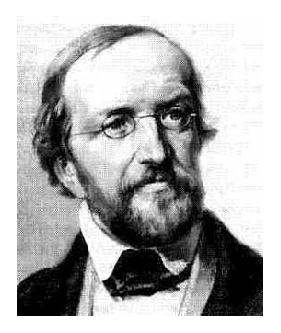
\includegraphics[width=3.5cm]{dirichlet.eps}
      \captionsetup{singlelinecheck=off,justification=raggedright}
\caption{Dirichlet}
    \end{minipage}\hspace{4mm}
    \begin{minipage}{.7\linewidth}
       Se trata de un concepto muy b�sico y general que comprende las distintas interpretaciones tradicionales de una funci�n como una tabla de valores, como una curva o como una f�rmula. Por todo ello, puede parecer sorprendente que dicho concepto, con su significado actual, sea muy reciente. Suele atribuirse al matem�tico alem�n \href{http://www-groups.dcs.st-and.ac.uk/~history/Biographies/Dirichlet.html}{Dirichlet} la definici�n, en 1837, del concepto moderno de funci�n. Antes de llegar aqu� hubo de recorrerse un largo camino que empieza con la publicaci�n en 1748 del libro de \href{http://es.wikipedia.org/wiki/Leonhard_Euler}{Leonhard Euler} \emph{Introductio in analysin infinitorum} en cuyo primer cap�tulo, titulado significativamente ``De Functionibus in genere'', esto es, ``Sobre las funciones en general'', Euler da la siguiente definici�n:\begin{quote}
\emph{Una funci�n de una cantidad variable es cualquier expresi�n anal�tica formada a partir de dicha cantidad variable y n�meros o cantidades constantes.}
\end{quote}
    \end{minipage}
  \end{figure}

Tambi�n fue Euler quien us� por primera vez la notaci�n $f(x)$ para indicar el valor de una funci�n $f$ en un valor $x$ de la variable. Euler no precisaba lo que entend�a por ``cualquier expresi�n anal�tica'' pero, sin duda, inclu�a las series, fracciones y productos infinitos y primitivas. Despu�s de dar esta definici�n, Euler distingue entre varios tipos de funciones seg�n que puedan o no representarse por medio de una sola expresi�n anal�tica.
 \begin{figure}[ht]
 \centering
     \begin{minipage}{.275\linewidth}
     \medskip
     \flushleft
      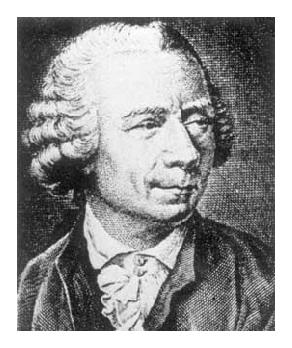
\includegraphics[width=3.5cm]{euler.eps}
      \captionsetup{singlelinecheck=off,justification=raggedright,margin={3mm,0mm}}
\caption{Euler}
    \end{minipage}
    \begin{minipage}{.7\linewidth}
      El libro de Euler \emph{Introductio in analysin infinitorum}, del que hay traducci�n al espa�ol, es considerado como el tercero m�s influyente en toda la historia de las matem�ticas (el primero ser�an los \emph{Elementos} de Euclides (300 adC) y el segundo los \emph{Principia} (1687) de Newton) y tuvo una amplia difusi�n.
      En el prefacio de dicho libro, Euler, afirmaba que el An�lisis Matem�tico es la ciencia general de las variables y sus funciones. Esto, que hoy d�a nos parece una evidencia, estaba muy lejos de serlo en el siglo XVIII. De hecho, matem�ticos como Newton, Leibniz, los hermanos Bernouilli y otros muchos en los siglos XVII y XVIII, se expresaban en t�rminos de curvas, superficies, �reas, l�neas tangentes.
    \end{minipage}
  \end{figure}

En el primer libro de C�lculo \emph{Analyse des infiniment petits, pour l'intelligence des lignes courbes} (L'H�pital, 1696), como ya se indica en su propio t�tulo, lo que se estudia son curvas, no funciones. Esto no tiene nada de extra�o. Los m�todos del C�lculo Infinitesimal eran todav�a muy recientes y sus razonamientos con frecuencia oscuros y confusos, por eso los matem�ticos de la �poca prefer�an fundamentar sus resultados geom�tricamente porque, desde Euclides, se hab�a considerado la geometr�a como el paradigma de la claridad y la perfecci�n l�gico -- deductiva.

La necesidad de precisar el concepto de funci�n surgi� poco despu�s, de forma muy natural, en el estudio de las vibraciones planas de una cuerda el�stica tensa, sujeta por sus extremos, cuya posici�n inicial en el plano viene dada por una funci�n conocida $\psi(x)$. D'Alembert (1749) y Euler (1750) obtuvieron esencialmente la misma soluci�n, pero discreparon sobre el tipo de funci�n inicial $\psi(x)$ permitida. Mientras que, seg�n D'Alembert, la posici�n inicial deb�a venir dada por una funci�n suave (derivable dos veces), Euler insist�a en que la evidencia f�sica impon�a la consideraci�n de funciones m�s generales (no derivables, con picos). �l mismo propuso como posici�n inicial de la cuerda una l�nea poligonal. Otro matem�tico, Daniel Bernouilli, propuso en 1753 una soluci�n del problema que ten�a como consecuencia que la funci�n $\psi(x)$ pod�a representarse como suma de una serie trigonom�trica infinita. Una situaci�n muy similar a �sta se produjo unos a�os despu�s, en 1822, como consecuencia de los trabajos de Jean B. Joseph Fourier sobre la propagaci�n del calor.

Los detalles de toda esta historia son muy interesantes pero imposibles de resumir en unas pocas l�neas y, adem�s, para poderlos entender hay que tener algunos conocimientos de An�lisis Matem�tico. En esencia, se trata de lo siguiente. En la segunda mitad del siglo XVIII y primera del XIX, al mismo tiempo que los matem�ticos segu�an considerando que las funciones deb�an ser continuas y derivables, salvo a lo sumo en una cantidad finita de ``puntos especiales'' (el mismo Euler ten�a esta idea), se estaban desarrollando m�todos para resolver problemas cada vez m�s complejos que permit�an representar ``funciones cualesquiera'' por medio de expresiones anal�ticas, principalmente, series de Fourier. Se supon�a que una representaci�n de este tipo deb�a ``transmitir su regularidad'' a la funci�n representada pero, por otra parte, �sta pod�a ser muy general. El coraz�n del problema estaba en la confusi�n de dos conceptos, aparentemente iguales pero muy distintos de hecho, el de funci�n y el de su representaci�n anal�tica. La separaci�n de estos conceptos llev� a considerar una funci�n con independencia de su representaci�n anal�tica. De esta forma una funci�n quedaba reducida a un conjunto de valores num�ricos completamente independientes asociados a una o varias variables, que es la idea subyacente a la definici�n moderna debida a Dirichlet (1837):
\begin{quote}
\small{``$y$ es una funci�n de una variable $x$, definida en un intervalo $a < x < b$, si para cada valor de la variable $x$ en este intervalo le corresponde un valor concreto de la variable $y$. Adem�s, es irrelevante la forma en la que esta correspondencia se establezca.''}
\end{quote}
Esta nueva idea de funci�n llev� a investigar nuevos tipos de funciones que, con frecuencia, ten�an un comportamiento inusual. En 1854 Riemann dio un ejemplo de funci�n integrable con infinitas discontinuidades en todo intervalo de longitud positiva. En 1872 Weierstrass sorprende a la comunidad matem�tica con una funci�n continua que no es derivable en ning�n punto. A estos ejemplos de funciones ``patol�gicas'' pronto les siguen otros. En el siglo XIX la necesidad de una fundamentaci�n rigurosa del An�lisis Matem�tico se hace evidente. El concepto de funci�n sigue en el centro de atenci�n y, aunque dicho concepto sigui� discuti�ndose casi hasta el final del siglo, hoy se reconoce a Dirichlet haber sido el primero en considerar seriamente la idea de funci�n como una ``correspondencia arbitraria''.

Para ampliar la informaci�n pueden visitarse los siguientes sitios en Internet.
\begin{list}{$\manoright$}{\addtolength{\itemsep}{-5pt}}
\item Sobre la evoluci�n del concepto de funci�n en\newline
\href{http://www.maa.org/pubs/Calc_articles/ma001.pdf}{http://www.maa.org/pubs/Calc_articles/ma001.pdf}.
\item \emph{Las series de Fourier y el desarrollo del An�lisis en el siglo XIX} por Fernando Bombal en \href{http://www.ma2.us.es/seminarios/four.pdf}{http://www.ma2.us.es/seminarios/four.pdf}.
\end{list}

\subsection{El desarrollo del �lgebra y la invenci�n de los logaritmos}
Con una calculadora de bolsillo, puedes hacer en una hora c�lculos que a un astr�nomo de los siglos XV o XVI le hubiesen llevado semanas o meses realizar. En aquella �poca hacer multiplicaciones, divisiones, calcular ra�ces cuadradas o potencias eran operaciones que requer�an mucho tiempo y esfuerzo. La explicaci�n de esto es que el desarrollo del �lgebra fue relativamente tard�o. El descubrimiento de las cantidades inconmensurables, y la carencia de una teor�a aritm�tica de las mismas, tuvo como consecuencia el abandono del �lgebra en favor de la Geometr�a. Se desarrollo as� una especie de ``�lgebra geom�trica'' en la que los n�meros se representaban por segmentos de l�nea y las operaciones aritm�ticas fueron sustituidas por construcciones geom�tricas. Las ecuaciones lineales y cuadr�ticas fueron resueltas con t�cnicas geom�tricas, evit�ndose as� el problema de las magnitudes inconmensurables. De esta forma en las matem�ticas griegas el razonamiento geom�trico lleg� a considerarse como el modelo de razonamiento matem�tico riguroso. Y as� sigui� siendo durante m�s de 2000 a�os.

Esta ``�lgebra geom�trica'' fue la causa del retraso en el desarrollo del �lgebra como disciplina independiente. Otra dificultad adicional estaba en el sistema de numeraci�n romano, un sistema de numeraci�n no posicional, que fue el utilizado en Occidente hasta el siglo XI. El sistema de numeraci�n decimal que actualmente usamos, el cero incluido, tuvo su origen en la India y lleg� a Occidente a trav�s de los �rabes, por eso los nuevos n�meros se llamaron ``n�meros ar�bigos''. La misma palabra ``�lgebra'' nace en el siglo IX y hace referencia al t�tulo del libro \emph{Hisab al-jabr w'al-muqabalah} del nombre de cuyo autor, el matem�tico Persa, \href{http://es.wikipedia.org/wiki/Muhammad_ibn_Musa_al-Jwarizmi}{Muhammad ibn-Musa al-Jwarizmi} (c.780-850),  deriva la palabra ``algoritmo''.

La paulatina adopci�n en toda Europa a lo largo de los siglos XI, XII y XIII de los ``n�meros ar�bigos'' supuso un extraordinario avance que propici� la expresi�n simb�lica de las operaciones aritm�ticas, inici�ndose as� el desarrollo del �lgebra como disciplina independiente de la Geometr�a\footnote{Nos referimos, claro est�, al �lgebra cl�sica, esto es, el estudio de las ecuaciones polin�micas y de la naturaleza y propiedades de sus ra�ces. El �lgebra moderna es el estudio de las estructuras axiom�ticas.}. En el siglo XV ya se usan en los c�lculos los n�meros negativos y las fracciones, pero los primeros progresos realmente notables no llegaron hasta el siglo XVI, gracias a los trabajos de matem�ticos como \href{http://es.wikipedia.org/wiki/Cardano}{Gerolamo Cardano} (1501-1576) que public� las soluciones de algunas ecuaciones de tercer y cuarto grado en su libro \emph{Ars magna} (1545), y \href{http://es.wikipedia.org/wiki/Fran\%C3\%A7ois_Vi\%C3\%A8te}{Fran\c{c}ois Vi�te} (1540-1603) que, entre otras cosas, propuso un sistema simb�lico que le permiti� representar de forma general distintos tipos de ecuaciones.

Hoy nos parece inconcebible una Matem�tica sin un lenguaje simb�lico apropiado, pero �ste se desarroll� lentamente a lo largo de los siglos XVI-XVII. Algunos de los siguientes datos est�n sacados del sitio Web \href{http://www.roma.unisa.edu.au/07305/symbols.htm}{The History of Mathematical Symbols}.
\begin{list}{\manoright}{\addtolength{\itemsep}{-5pt}}
\item La primera aparici�n impresa de los s�mbolos $+$ y $-$ fue en la aritm�tica de John Widmann, publicada in 1489 in Leipzig.
El autor del primer libro de texto sobre �lgebra en lengua alemana impreso en 1525, Christoff Rudolff, usa estos s�mbolos con su significado actual. Durante mucho tiempo se usaron solamente en �lgebra antes de que se generalizara su uso en aritm�tica.
\item Hab�a una gran variedad de s�mbolos para la multiplicaci�n. Fue el matem�tico ingl�s William Oughtred quien en su obra \emph{Clavis Mathematicae}, publicada en 1631, dio al s�mbolo $\times$ el significado que tiene hoy d�a.
\item El signo para la igualdad que usamos actualmente fue introducido por el matem�tico y m�dico ingl�s Robert Recorde en su libro \emph{The Whetstone of Witte} (1557). No fue inmediatamente aceptado pues, como ocurr�a con gran parte de la notaci�n matem�tica de este per�odo, cada uno ten�a su propio sistema, pero hacia 1700 el signo $=$ era ya de uso general.
\item Aunque las fracciones decimales eran conocidas desde antiguo, no eran usadas con frecuencia debido a la  confusa notaci�n empleada para representarlas. Fue Neper quien introdujo en 1616 el separador decimal (coma o punto), lo que facilit� mucho el uso de las fracciones decimales.
\item Los s�mbolos para las desigualdades, $<$ y $>$, con su significado actual fueron introducidos por el matem�tico ingl�s Thomas Harriot (1560-1621) en su obra \emph{Artis Analyticae Praxis} publicada en Londres en 1631.
\end{list}
En el siglo XV la trigonometr�a esf�rica fue adquiriendo cada vez mayor importancia por sus aplicaciones para la navegaci�n astron�mica, en la cual debe resolverse un tri�ngulo esf�rico para trazar la ruta del nav�o. Para facilitar los c�lculos, se
elaboraron numerosas tablas trigonom�tricas en las que trabajaron matem�ticos como Cop�rnico (1473-1543), Tycho Brahe (1546-1601), Kepler (1571-1630) y otros. Los c�lculos para la realizaci�n de estas tablas eran largos y penosos. En este contexto tuvo lugar la invenci�n de los logaritmos por John Neper.

\begin{figure}[ht]
    \begin{minipage}{.35\linewidth}
      
\includegraphics[width=4cm]{napier.eps}
      \captionsetup{singlelinecheck=off,justification=raggedright}%,margin={3mm,0mm}
\caption{John Napier}
    \end{minipage}%\hspace{1cm}%
    \begin{minipage}{.65\linewidth}
     John Napier o Neper introdujo los logaritmos en su libro \emph{Mirifici Logarithmorum Canonis Descriptio} (1614). Este trabajo ten�a treinta y siete p�ginas explicando la naturaleza de los logaritmos y noventa p�ginas de tablas de logaritmos de funciones trigonom�tricas en las que Neper trabaj� durante 20 a�os antes de publicar sus resultados. En el a�o 1615 el matem�tico ingl�s Henry Briggs (1561-1630)  visit� a Neper en Edimburgo, y le convenci� para modificar la escala inicial usada por �ste. Nacieron as� los logaritmos de base 10 que fueron divulgados por el f�sico alem�n Kepler, extendi�ndose su uso en relativamente poco tiempo por toda Europa.
\end{minipage}
  \end{figure}
  Al principio, Neper llam� a los exponentes de las potencias ``numeros artificiales'', pero m�s tarde se decidi� por la palabra logaritmo, compuesta por los t�rminos griegos \emph{logos} (raz�n) y \emph{aritmos} (n�mero).
  \begin{quote}
\emph{Los logaritmos son n�meros, que se descubrieron para facilitar la soluci�n de los problemas aritm�ticos y geom�tricos, a trav�s de esto se evitan todas las complejas multiplicaciones y divisiones transform�ndolo a algo completamente simple a trav�s de la substituci�n de la multiplicaci�n por la adici�n y la divisi�n por la substracci�n. Adem�s el c�lculo de las ra�ces se realiza tambi�n con gran facilidad.}\vspace{-3mm}
\vspace{-6mm}
\begin{flushright}
Henry Briggs
\end{flushright}%\flushright{Henry Briggs}
\end{quote}
Los logaritmos pasaron a ser una herramienta muy valorada, en especial entre los astr�nomos. Laplace se refiere a esto en la siguiente frase.
\begin{quote}
\emph{Con la reducci�n del trabajo de varios meses de c�lculo a unos pocos d�as, el invento de los logaritmos parece haber duplicado la vida de los astr�nomos.}\vspace{-3mm}
\begin{flushright}
Pierre Simon Laplace
\end{flushright}
\end{quote}
\section{Lo que debes haber aprendido en este cap�tulo}
\begin{list}{$\bullet$}{\addtolength{\itemsep}{-5pt}}
\item El concepto de funci�n y el formalismo que usamos para definir una funci�n.
\item Las operaciones con funciones. La composici�n de funciones.
\item Los conceptos de funci�n mon�tona y de inversa de una funci�n inyectiva.
\item Las definiciones y propiedades principales de las funciones logar�tmicas y exponenciales.
\item Las definiciones y propiedades principales de las funciones trigonom�tricas.
\item Las definiciones y propiedades principales de las funciones arcoseno, arcocoseno y arco\-tan\-gente.
\item Las definiciones y propiedades principales de las funciones hiperb�licas y sus inversas.
\end{list}

Como lectura adicional te recomiendo los cap�tulos 3 y 4 del libro de Michael Spivak \cite{spivak}.



\chapter{N�meros complejos. Exponencial compleja}
\vspace*{-1cm}
\begin{flushright}
{\small \textit{El camino m�s corto entre dos verdades del an�lisis \\ real pasa con
 frecuencia por el an�lisis complejo.} \\  Jaques Hadamard}
\end{flushright}

\section{Un poco de historia}
Los n�meros que hoy llamamos
``complejos'' fueron durante muchos a\~{n}os motivo de
pol�micas y controversias entre la comunidad cient�fica.
Poco a poco, por la creciente evidencia de su utilidad, acabaron
por ser com�nmente aceptados, aunque no fueron bien
comprendidos hasta �pocas recientes. Nada hay de extra\~{n}o
en ello si pensamos que los n�meros negativos no fueron
plenamente aceptados hasta finales del siglo XVII.

Los n�meros complejos hacen sus primeras t�midas
apariciones en los trabajos de Cardano (1501-1576) y Bombelli
(1526-1672) relacionados con el c�lculo de las ra�ces de
la c�bica o ecuaci�n de tercer grado. Fue Ren�
Descartes (1596-1650) quien afirm� que \textit{``ciertas
ecuaciones algebraicas s�lo tienen soluci�n en nuestra
imaginaci�n''} y acu\~{n}� el calificativo
\textit{``imaginarias''} para referirse a ellas. Desde el siglo
XVI hasta finales del siglo XVIII los n�meros complejos o
imaginarios son usados con recelo, con desconfianza. Con
frecuencia, cuando la soluci�n de un problema resulta ser un
n�mero complejo se interpreta esto como que el problema no
tiene soluci�n. Para Leibniz \textit{``el n�mero
imaginario es un recurso sutil y maravilloso del esp�ritu
divino, casi un anfibio entre el ser y el no ser.''}

Las razones de todo esto son claras. As� como los n�meros
reales responden al problema bien cotidiano de la medida de
magnitudes, no ocurre nada similar con los n�meros complejos.
Mientras los matem�ticos necesitaron interpretar en
t�rminos f�sicos sus objetos de estudio, no se avanz�
mucho en la comprensi�n de los n�meros complejos.

El �xito de Euler y Gauss al trabajar con n�meros
complejos se debi� a que ellos no se preocuparon de la
\textit{``naturaleza''} de los mismos; no se preguntaron
``?`qu� es un n�mero complejo?'', sino que se dijeron
\textit{``a ver, para qu� sirven, qu� puede hacerse con
ellos''}. Es Gauss quien definitivamente concede a los n�meros
complejos un lugar privilegiado dentro de las matem�ticas al
probar en 1799 el resultado conocido como \emph{Teorema
Fundamental del �lgebra} que afirma que toda ecuaci�n
polin�mica de grado $n$ con coeficientes complejos tiene, si
cada ra�z se cuenta tantas veces como su orden, $n$
ra�ces que \textit{tambi�n son n�meros complejos}. Merece la pena que entiendas bien lo que afirma este resultado. F�jate en cada una de las
ecuaciones:
$$x+3=0,\quad 2x +
3=0,\quad   x^2-2=0,\quad x^2+2x+2=0$$ Cuyas soluciones
$$x=-3,\quad x=-3/2,\quad x=\pm\sqrt{2},\quad x=-1\pm i$$ tienen sentido cuando $x$
es, respectivamente, un n�mero entero, racional, real o
complejo. Podr�a ocurrir que este proceso de ampliaci�n
del campo num�rico continuara. ?`Qu� ocurrir� si ahora
consideramos ecuaciones polin�micas con coeficientes
complejos? Por ejemplo: $$ x^5+(1-i)x^4+(1/5 -
i\sqrt{2})x^2-8x+3-i/\sqrt{3}=0$$ ?`C�mo ser�n sus
soluciones? ?`Aparecer�n tambi�n nuevos tipos de
n�meros? El Teorema Fundamental del �lgebra nos dice que
esa ecuaci�n tiene soluciones que \textit{tambi�n} son
n�meros complejos y, por tanto, que no aparecer�n ya por
este procedimiento nuevos tipos de n�meros.

El t�rmino, hoy usado de \textit{``n�meros complejos''} se
debe a Gauss, quien tambi�n hizo popular la letra ``$i$'' que
Euler (1707-1783) hab�a usado espor�dicamente. En 1806
Argand interpreta los n�meros complejos como vectores en el
plano. La fecha de 1825 es considerada como el nacimiento de la
teor�a de funciones de variable compleja, pues se publica en
dicho a\~{n}o la Memoria sobre la Integraci�n Compleja que
Cauchy hab�a escrito ya en 1814.

Los n�meros complejos son una
herramienta b�sica de c�lculo. Son especialmente �tiles para
trabajar con funciones sinusoidales, y por eso se hace uso constante
de ellos siempre que representamos una se�al por medio de dichas
funciones, y no hay que olvidar que �se es el prop�sito b�sico de
los \emph{``m�todos de Fourier''}. La \emph{Transformada de Fourier
Discreta}, una herramienta fundamental en el tratamiento digital de
se�ales, toma valores complejos. Las \emph{transformadas de Fourier
y de Laplace} son funciones complejas. La \emph{transformada $z$},
al igual que otras transformadas de uso frecuente, se define como
una serie de n�meros complejos. La funci�n exponencial compleja
desempe�a un papel fundamental en el estudio de los sistemas LTI
(sistemas lineales invariantes en el tiempo) y tambi�n en la teor�a
de las ecuaciones diferenciales lineales.

\section{Operaciones b�sicas con n�meros complejos}
\begin{definicion} Consideremos en el conjunto \Rx{2}\ las
operaciones de adici�n y producto definidas por
\begin{eqnarray}
(x, y) + (u, v) & = & (x + u, y + v) \label{sumacompleja}\\
(x, y)(u, v) & =  & (xu - yv, xv + yu)\label{productocomplejo}
\end{eqnarray}
Es muy f�cil comprobar las propiedades asociativa, conmutativa y
distributiva de las operaciones as� definidas. El elemento neutro de
la suma es $(0,0)$ y $(1,0)$ es la unidad del producto. Adem�s,
$(-x,-y)$ es el opuesto de $(x,y)$, y todo
 $(x,y)\neq (0,0)$ tiene inverso
 $$\,(x,y)\left(\dfrac{x}{x^2+y^2},\dfrac{-y}{x^2+y^2}\right)=(1,0)$$
Todas estas propiedades se resumen diciendo que $(\Rx{2},+,\cdot)$
(l�ase ``el conjunto \Rx{2}\ con las operaciones de adici�n y
producto'') es un \emph{cuerpo}. Dicho cuerpo se representa
simb�licamente por \C\ y sus elementos se llaman \textit{n�meros
complejos}.
\end{definicion}

\subsection{Comentarios a la definici�n de n�mero complejo}
No debes olvidar que cada concepto matem�tico tiene sentido dentro de una determinada estructura. Con frecuencia, cuando sobre un mismo conjunto hay definidas varias estructuras, la terminolog�a que se usa indica la estructura a la que nos referimos. Eso pasa en \Rx{2}\ donde conviven varias estructuras cada una con su terminolog�a propia. Usualmente en $\R^2$ se consideran las siguientes estructuras.
\begin{list}{$\bullet$}{\addtolength{\itemsep}{-5pt}}
\item Ninguna. Es decir, solamente consideramos que $\R^2$ es un conjunto. En tal caso llamamos a sus elementos \emph{pares ordenados de n�meros reales}.
\item La estructura de espacio vectorial. Esto es, vemos $\R^2$ como un espacio vectorial real. En tal caso a sus elementos los llamamos \emph{vectores}.
\item La estructura de espacio eucl�deo que se obtiene a�adiendo a la estructura de espacio vectorial la distancia eucl�dea definida por el producto escalar usual. Esto es, vemos $\R^2$ como el plano eucl�deo de la geometr�a elemental. En este caso a sus elementos los llamamos \emph{puntos}. La misma terminolog�a se emplea cuando se considera en $\R^2$ la estructura de espacio af�n o de espacio topol�gico.
\item La estructura de cuerpo definida por las operaciones (\ref{sumacompleja}) y (\ref{productocomplejo}). En tal caso, a los elementos de $\R^2$ se les llama \emph{n�meros complejos}.
\end{list}
Ocurre que estos t�rminos se usan a veces en un mismo
p�rrafo lo que puede resultar confuso. La regla que debes tener
siempre presente es que todo concepto matem�tico tiene
sentido propio dentro de una determinada estructura
matem�tica. Por ello, a un elemento de \Rx{2}\ se le llama n�mero
complejo cuando se va a usar el producto definido en (\ref{productocomplejo}) que es lo
que en realidad distingue a los n�meros complejos de los vectores
de \Rx{2}.

\subsection{Forma cartesiana de un n�mero complejo}
El s�mbolo usual $(x,y)$ para representar pares ordenados no es
conveniente para representar el n�mero complejo $(x,y)$. Para
convencerte calcula, usando la definici�n (\ref{productocomplejo}), $(1,-1)^4$. Representaremos los n�meros
complejos con un simbolismo m�s apropiado en el que va a intervenir el producto complejo. Para ello, observa que:
\[
    \begin{split}
        (x, 0) + (y, 0) &= (x + y, 0) \\
        (x, 0)(y, 0) &=  (x y, 0)
    \end{split}
\]
Esto indica que los n�meros complejos de la forma $(x, 0)$ se comportan respecto a la
suma y la multiplicaci�n de n�meros complejos exactamente de la misma forma que lo
hacen los n�meros reales respecto a la suma y multiplicaci�n propias. En t�rminos m�s
precisos, $\R\times\{0\}$ es un subcuerpo de \C\ isomorfo a \R. Por esta raz�n, en las
operaciones con n�meros complejos podemos sustituir los complejos del tipo $(x,0)$ por
el n�mero real $\,x$. Es decir, hacemos la identificaci�n $(x,0)=x$.

F�jate que con dicha identificaci�n el producto $\,x(u,v)\,$ tiene dos posibles
interpretaciones: producto del escalar real $\,x\,$ por el vector $\,(u,v)$ (estructura
vectorial de \Rx{2}) y producto del complejo $\,(x,0)\,$ por el complejo $\,(u,v)$.
Pero ambos coinciden y son iguales a $(x u,x v)$.

El n�mero complejo $(0, 1)$ lo representaremos por $i$ y lo llamaremos \emph{unidad
imaginaria}. Con ello tenemos que
$$ i^2 = (0,1)(0,1) = (-1,0) = -1$$ Ahora podemos escribir
$$
(x, y) = (x, 0) + (0, y)=(x, 0) + (0, 1)(y,0) = x + i y
$$
Se dice que $x+i y$ es la \emph{expresi�n cartesiana} (tambi�n se le llama \emph{expresi�n bin�mica}) del n�mero complejo $(x,y)$.  El producto ahora es
muy f�cil de recordar pues
$$(x+i y)(u+i v)=x u + i^2 y v+i(x v + y u)= x u - y v + i(x v + y u)$$
\begin{definicion}
Se dice que $\,x\,$ es la \emph{parte real}\index{parte real} e $\,y\,$ es la \emph{parte
imaginaria}\index{parte imaginaria} del n�mero complejo $x+i y$.
\end{definicion}
Naturalmente, dos n�meros complejos son iguales cuando
tienen igual parte real e igual parte imaginaria.

\noindent\textbf{Notaci�n.} Es costumbre representar los n�meros complejos con las letras
$\,z$ y  $\,w$ y reservar las letras $\,x$, $y$, $u$, $v$ para
representar n�meros reales. Una expresi�n de la forma
$z=x+iy$ se interpreta como que $z$ es el n�mero complejo cuya
parte real es $x$ y cuya parte imaginaria es $y$. Se escribe
$\re(z)$ e $\im(z)$ para representar las partes real e imaginaria
de $z$.

\subsection{Comentarios a la definici�n usual $\,i=\sqrt{-1}$}
Acabamos de ver que $i^2=-1$ pero eso no nos permite escribir as�,
sin m�s ni m�s, que $i=\sqrt{-1}$. F�jate lo que ocurre si ponemos
$i=\sqrt{-1}$ y manejamos ese s�mbolo con las reglas a las que
estamos acostumbrados:
$$
-1=i^2=i\,i=\sqrt{-1}\sqrt{-1}=\sqrt{(-1)(-1)}=\sqrt{1}=1$$ Luego
$1=-1$. Por tanto, las matem�ticas son contradictorias y
aqu� hemos acabado.

Naturalmente, el error procede de que estamos haciendo disparates.
F�jate que en la expresi�n $\sqrt{-1}$ \emph{no puedes interpretar
que $-1$ es el n�mero real $-1$} (porque, como sabes, los n�meros
reales negativos no tienen ra�z cuadrada real), \emph{sino que
tienes que interpretar $-1$ como el n�mero complejo $-1$} (espero
que ya tengas clara la diferencia). Resulta as� que estamos usando
ra�ces de n�meros complejos \emph{sin haberlas definido y dando
por supuesto que dichas ra�ces verifican las mismas propiedades que
las de los n�meros reales positivos}.

\emph{Antes} de escribir $\sqrt{-1}$ hay que definir qu� significa
$\sqrt{z}$ para $z\en\C$. Cuando lo hagamos veremos �sorpresa! que
\emph{la igualdad} $\sqrt{z}\sqrt{w}=\sqrt{z w}$, v�lida cuando
$z,w\in\Rp$, \emph{no es cierta en general cuando} $z,w\in\C$.

Todav�a m�s disparatado es \emph{definir} $i=\sqrt{-1}$ sin ni
siquiera haber definido antes los n�meros complejos. Sin embargo,
y aunque parezca mentira, en muchos textos se define (porque s�,
sin m�s explicaciones) $\,i=\sqrt{-1}$ y a continuaci�n se dice
que los n�meros de la forma $a+ib$ son los n�meros complejos. No
es de extra�ar que luego resulte que $1=-1$. Todav�a pueden hacerse peor las cosas. Recientemente he encontrado en un texto de una instituci�n de educaci�n a distancia escrito por varios profesores la siguiente asombrosa definici�n: $\,i=+\sqrt{-1}$.

\subsection{No hay un orden en \C\ compatible con la estructura
algebraica}
Al ampliar \R\ a \C\ ganamos mucho pero tambi�n perdemos algo. Te
recuerdo que \R\ tiene dos estructuras: la algebraica y la de orden.
Ambas estructuras est�n armoniosamente relacionadas. Pues bien, en
\C\ no hay nada parecido. Podemos definir relaciones de orden en \C,
pero no hay ninguna de ellas que sea compatible con la estructura
algebraica. Es decir, es imposible definir un concepto de n�mero
complejo positivo de forma que la suma y el producto de complejos
positivos sea positivo. Por ello no se define en \C\ ning�n orden.
As� que ya sabes: �nunca escribas desigualdades entre n�meros
complejos! Naturalmente, puedes escribir desigualdades entre las
partes reales o imaginarias de n�meros complejos, porque tanto la
parte real como la parte imaginaria de un n�mero complejo son
n�meros reales.

\section{Representaci�n gr�fica. Complejo conjugado y
m�dulo}
Es usual representar el n�mero complejo $z=x + i y$ como el vector del
plano $(x,y)$ y, en ese sentido, se habla del \emph{plano complejo}.
El eje horizontal recibe el nombre de \emph{eje real}, y el eje
vertical recibe el nombre de \emph{eje imaginario}.

\begin{figure}[ht]
\centering
\begin{pspicture}(-.5,-2.5)(4,2.5)
\psaxes[labels=none,ticks=none,linewidth=.6pt,arrowscale=1.7]{->}(0,0)(-.5,-2.5)(4,2.5)[$X$,0][$Y$,0]
\psset{arrowscale=2}
\psline[linewidth=1pt]{->}(0,0)(2,2)
\psline[linestyle=dashed,linewidth=.5pt](0,2)(2,2)(2,0)
\psline[linestyle=dashed,linewidth=.8pt]{->}(0,0)(2,-2)
\uput[d](2,0){$x$}
\uput[l](0,2){$y$}
\uput[r](2,2){$z=x+iy$}
\uput[r](2,-2){$\conj{z}=x-iy$}
\uput[u](1,1){$\abs{z}$}
\end{pspicture}
\caption{Representaci�n de un n�mero complejo
\label{fig:numero_complejo}}
\end{figure}

Si $z = x + iy$ es un n�mero complejo (con $x$ e $y$ reales),
    entonces el \textbf{conjugado} de $z$ se define como:
$$
\conj{z} = x - iy
$$
y el  \textbf{m�dulo} o \textbf{valor absoluto} de $z$, se define
como:
$$
\abs{z} = \sqrt{x^2 + y^2}
$$
Observa que $\sqrt{x^2 + y^2}$ est� definido sin ambig�edad; es la
ra�z cuadrada del n�mero real no negativo $x^2 + y^2$.

Geom�tricamente, $\conj{z}$ es la reflexi�n de $z$ respecto al eje
real, mientras que $\abs{z}$ es la distancia eucl�dea del punto
$(x,y)$ a $(0, 0)$ o, tambi�n, la longitud o \textbf{norma eucl�dea}
del vector $(x,y)$ (ver figura \ref{fig:numero_complejo}). La
\textbf{distancia} entre dos n�meros complejos $z$ y $w$ se define
como $\abs{z - w}$ y es la distancia eucl�dea entre los respectivos puntos del plano.

La representaci�n gr�fica de la suma es la usual para la suma de vectores. Dos n�meros complejos $z = x+iy$ y $w = u+iv$ determinan un paralelogramo cuya
diagonal (ver figura \ref{fig:suma}) es $z + w$ (la otra diagonal es $z-w$).
\begin{figure}[ht]
\centering
\psset{unit=1.5cm}
\begin{pspicture}(-.2,-.2)(4,4)
\psaxes[labels=none,ticks=none,linewidth=.6pt,arrowscale=1.7]{->}(0,0)(-.2,-.2)(4,4)[$X$,0][$Y$,0]
\psset{arrowscale=2}
\psline[linewidth=1pt]{->}(0,0)(1,2)
\psline[linewidth=1pt]{->}(0,0)(2,1)
\psline[linewidth=1pt]{->}(0,0)(3,3)
\psline[linestyle=dashed,linewidth=.5pt](1,2)(3,3)(2,1)
\psline[linestyle=dashed,linewidth=.5pt](1,2)(1,0)
\psline[linestyle=dashed,linewidth=.5pt](2,1)(2,0)
\psline[linestyle=dashed,linewidth=.5pt](3,3)(3,0)
\uput[26.5](2,1){$w$}
\uput[d](2,0){$u$}
\uput[45](3,3){$z+w$}
\uput[d](1,0){$x$}
\uput[d](3,0){$x+u$}
\uput[63.4](1,2){$z$}
\end{pspicture}
\caption{Suma de n�meros complejos \label{fig:suma}}
\end{figure}

Las siguientes propiedades de la conjugaci�n compleja son de comprobaci�n muy sencilla.
\begin{proposicion}
Cualesquiera sean los n�meros complejos $z$ y $w$ se
verifica que:
\begin{equation}
\conj{\conj{z}}=z,\quad\conj{z+w}=\conj{z}+\conj{w},\quad \conj{zw}=\conj{z}\conj{w}.
\end{equation}
\end{proposicion}

El siguiente resultado establece las principales propiedades del m�dulo de un n�mero complejo. Como ver�s son muy parecidas a las propiedades del valor absoluto y su demostraci�n es pr�cticamente la misma.
\begin{teorema}
Cualesquiera sean los n�meros complejos $z,w\in\C$ se verifica que:
\begin{enumerate}[a)]
\item \begin{equation}\label{desigualdadbasica}
\max\{\abs{\re z},\abs{\im z}\}\leqslant
    \abs{z}\leqslant\abs{\re z}+\abs{\im z}
\end{equation}
En particular, $\re z=\abs{z}$ si, y s�lo si, $z\en\Rpo$.
\item El m�dulo de un producto es igual al producto de los m�dulos.
\begin{equation}\label{moduloproducto}
\abs{z w} = \abs{z} \abs{w}
\end{equation}
\item El m�dulo de una suma es menor o igual que la suma de los m�dulos.
\begin{equation}
\abs{z + w} \leqslant \abs{z} + \abs{w}\qquad \textrm{(desigualdad triangular)}
\end{equation}
La desigualdad triangular es una igualdad si, y solamente si, alguno de los n�meros es cero o uno de ellos es un m�ltiplo positivo del otro; equivalentemente, est�n en una misma semirrecta a partir del origen.
\end{enumerate}
\end{teorema}
\dem La demostraci�n de a) es inmediata. Para demostrar b) y c) usaremos la igualdad
 $\,\abs{z}^2=z\conj{z}\,$ que se deduce directamente
de la definici�n de m�dulo de un n�mero complejo, y la estrategia (\ref{estrategiadesigualdadpositivos}) que ya usamos para probar las propiedades an�logas del valor absoluto.

b) Basta observar que $\abs{z w}$ y $\abs{z} \abs{w}$ son n�meros positivos cuyos cuadrados coinciden, pues
$$\abs{z w}^2=zw\conj{zw}=zw\conj{z}\conj{w}=z\conj{z}w\conj{w}=\abs{z}^2\abs{w}^2=(\abs{z}\abs{w})^2$$
c) Es suficiente probar que $\abs{z+w}^2\leqslant(\abs{z}+\abs{w})^2$. En efecto:
$$
\begin{aligned}
\abs{z+w}^2 &
=(z+w)\conj{(z+w)}=(z+w)(\conj{z}+\conj{w})=z\conj{z}+w\conj{w}+z\conj{w}+\conj{z}w=\\
&=\abs{z}^2+\abs{w}^2+2\re{(z\conj{w})}\leqslant\abs{z}^2+\abs{w}^2+2\abs{\re{(z\conj{w})}}\leqslant\\
&\leqslant
\abs{z}^2+\abs{w}^2+2\abs{z\conj{w}}=\abs{z}^2+\abs{w}^2+2\abs{z}\abs{\conj{w}}=\abs{z}^2+\abs{w}^2+2\abs{z}\abs{w}=\\
&=(\abs{z}+\abs{w})^2
\end{aligned}
$$
Evidentemente, si $z=0$ o si $w=0$, se verifica la igualdad. Supongamos que $z\neq 0$ y $w\neq 0$. De lo anterior deducimos que se verifica la igualdad
$\abs{z+w}=\abs{z}+\abs{w}$ si, y s�lo si, $\re{z\conj{w}} =\abs{z\conj{w}}$, esto es, si $z\conj{w} \in \Rp$, o lo que es lo
mismo $z\conj{w} = \rho$ donde $\rho \en \Rp$. Esta igualdad,
puede escribirse de forma equivalente, multiplicando por $w$, como
$z\abs{w}^2 = \rho w$; y dividiendo ahora por $\abs{w}^2$, obtenemos  $z = \lambda w$ para alg�n
$\lambda\in\Rp$, lo que quiere decir que $z$ y $w$ est�n en
una misma semirrecta a partir del origen.\fin

\noindent{\textbf{Observaci�n.}}\
Para expresar un cociente de complejos en forma cartesiana se multiplica numerador y denominador por el conjugado del denominador:
$$
\frac{u+iv}{x+i y}=\frac{(u+iv)(x-iy)}{x^2+y^2}=\frac{ux+vy}{x^2+y^2}+i\frac{vx-uy}{x^2+y^2}.
$$

\subsection{Forma polar y argumentos de un n�mero complejo}
El uso de coordenadas polares en el plano facilita mucho los
c�lculos con productos de n�meros complejos. Para cualquier n�mero
complejo $z=x+iy \neq 0$ podemos escribir
$$ z = \abs{z} \left(\dfrac{x}{\abs{z}}+i\dfrac{y}{\abs{z}}\right) $$
Como $\left(\dfrac{x}{\abs{z}},\dfrac{y}{\abs{z}}\right)$ es un punto de la
circunferencia unidad, puede escribirse en la forma
$$\left(\dfrac{x}{\abs{z}},\dfrac{y}{\abs{z}}\right)=(\cos\vartheta,\sen\vartheta)$$
para alg�n n�mero $\vartheta\en\R$. Resulta as� que
$$z=\abs{z}(\cos\vartheta+i\sen\vartheta)$$
Esta forma de expresar un n�mero complejo recibe el nombre de
\textbf{forma polar}, cuya interpretaci�n gr�fica vemos en la figura
(\ref{fig:forma_polar}).

\begin{figure}[ht]
\centering
\psset{unit=2cm}
\begin{pspicture}(-.2,-.2)(3,3)
\psaxes[linewidth=.6pt,labels=none,ticks=none,arrowscale=2]{->}(0,0)(-.2,-.2)(3,3)[$X$,0][$Y$,0]
\psset{arrowscale=2,arrowinset=.6}
\psline[linewidth=1pt]{->}(0,0)(2,2)
\psarc[linewidth=.5pt](0,0){1}{0}{45}
\SpecialCoor
\uput[r](1;22){$\vartheta$}
\uput[u](1,1){$\abs{z}$}
\end{pspicture}
\caption{Forma polar de un n�mero complejo \label{fig:forma_polar}}
\end{figure}

Dado $z\en\C$, $z\neq 0$, hay infinitos n�meros $t\en\R$ que
verifican la igualdad $z=\abs{z}(\cos t,\sen t)$ cualquiera de
ellos recibe el nombre de \textbf{argumento} de $z$. El conjunto de
todos los argumentos de un n�mero complejo no nulo se representa por
$\Arg(z)$. $$\psframebox{\ \Arg(z)=\set{t\en\R : z=\abs{z}(\cos t+i\sen t)}\ }$$
Observa que
$$s,\,t\en\Arg(z)\Longleftrightarrow\left\{\begin{aligned}\cos(t)&=\cos(s)\\
\sin(t)&=\sin(s)\end{aligned}\right\}\Longleftrightarrow s=t +
2k\pi\ \ \textrm{para alg�n}\ \ k\en\Z$$ Por tanto, conocido un
argumento $t_0\en\Arg(z)$ cualquier otro es de la forma $t_0+2k\pi$
para alg�n $k\en\Z$, es decir, $\Arg(z)=t_0+2\pi\Z$.

De entre todos los argumentos de un n�mero complejo $z\neq 0$ hay
uno �nico que se encuentra en el intervalo $]-\pi, \pi]$, se
representa por $\arg(z)$ y se le llama \textbf{argumento principal}
de $z$. No es dif�cil comprobar (v�ase el ejercicio resuelto (\ref{formulaargumentoprincipal})) que el argumento principal de
$z=x+iy\neq 0$ viene dado por:
$$
\cajadoble{
\arg(z)=\begin{cases}\arctg(y/x)-\pi \ \ \textrm{si $y<0$, $x<0$}\\ -\pi/2\ \ \textrm{si $y<0$, $x=0$}\\
\arctg(y/x)\ \ \textrm{si $x>0$}\\ \pi/2\ \ \textrm{si $y>0$,
$x=0$}\\ \arctg(y/x)+\pi \ \ \textrm{si $y\geqslant 0$,
$x<0$}\end{cases}}
$$

\subsubsection*{Igualdad de dos n�meros complejos en forma polar}
Para que dos n�meros complejos escritos en forma polar $z=\abs{z}(\cos\vartheta+i\sen\vartheta)$ y \linebreak $w=\abs{w}(\cos\varphi+i\sen\varphi)$, sean iguales es condici�n necesaria y suficiente que los m�dulos sean iguales $\abs{z}=\abs{w}$, y los argumentos sean iguales, $\Arg(z)=\Arg(w)$, y �sta condici�n equivale a que $\vartheta-\varphi$ sea un m�ltiplo entero de $2\pi$.
$$
\abs{z}(\cos\vartheta+i\sen\vartheta)=\abs{w}(\cos\varphi+i\sen\varphi)\Longleftrightarrow\left\{
                                                                                            \begin{array}{rcl}
                                                                                              \abs{z}&=&\abs{w} \\
                                                                                              \vartheta-\varphi&=& 2m\pi\quad (m\en\Z)
                                                                                            \end{array}
                                                                                          \right.
$$
\subsection{Observaciones a la definici�n de argumento
principal}

Puede parecer un poco extra�a la forma de elegir el argumento
principal de un n�mero complejo. La elecci�n que hemos hecho
supone que medimos �ngulos en el semiplano superior de $0$ a
$\pi$ y en el semiplano inferior de $0$ a $-\pi$.

\begin{figure}
\vspace*{1cm}
\centering
\begin{pspicture}(-2.5,-2.5)(2,2)
\psset{unit=1.5cm}
\psaxes[linewidth=.6pt,labels=none,ticks=none](0,0)(-2.5,-1.5)(1.2,1.5)%[$X$,90][$Y$,90]
\psset{arrowscale=1.5}
\psarc[linewidth=.6pt]{->}(0,0){.9}{0}{170}
\psarc[linewidth=.6pt]{<-}(0,0){.9}{190}{360}
\psset{arrowscale=2,arrowinset=.6}
\psline[linewidth=1pt]{->}(0,0)(2;170)
\psline[linewidth=1pt]{->}(0,0)(2;190)
\uput[u](2;170){\scalefont{.8}$w=x+iv$}
\uput[d](2;190){\scalefont{.8}$z=x+iy$}
\uput[r](0,1.2){$\frac{\pi}{2}$}
\uput[r](0,-1.2){$-\frac{\pi}{2}$}
\uput[u](-2.2,0){\scalefont{.8}$\pi$}
\uput[d](-2.2,0){\scalefont{.8}$-\pi$}
\uput[r](1.3,0){\psframebox{\scalefont{.8}$\arg(z)=\arctg(y/x)$}}
\uput[l](-.85,1){\psframebox{\scalefont{.8}$\arg(z)=\arctg(y/x)+\pi$}}
\uput[l](-.85,-1){\psframebox{\scalefont{.8}$\arg(z)=\arctg(y/x)-\pi$}}
\end{pspicture}
\caption{Argumento principal}
\end{figure}

F�jate que si tomas un n�mero complejo que est� situado en el tercer
cuadrante $z=x+iy$ con $x<0,y<0$ y supones que $\,y\,$ es pr�ximo a
$0$, su argumento principal est� pr�ximo a $-\pi$, y si tomas un
n�mero complejo que est� situado en el segundo cuadrante, $w=x+iv$
con $x<0,v>0$, y supones que $\,v\,$ es pr�ximo a $0$, su argumento
principal est� pr�ximo a $\pi$. Adem�s, la distancia
$\abs{w-z}=\abs{v-y}=v-y$ es tan peque�a como quieras. Esto nos dice
que el argumento principal tiene una discontinuidad en el eje real
negativo: salta de $-\pi$ a $\pi$ cuando atravesamos dicho eje desde
el tercer al segundo cuadrante.

Peor todav�a dir�s. Hasta cierto punto. Primero, la discontinuidad es inevitable. Si
queremos elegir argumentos en un intervalo de longitud $2\pi$, digamos
$[\alpha,\alpha+2\pi[$, entonces dichos argumentos saltan de $\alpha$ a $\alpha+2\pi$
cuando atravesamos la semirrecta $(x,y)=\rho(\cos\alpha,\sen\alpha)$, $(\rho>0)$. En
particular, si tomamos argumentos en el intervalo $[0,2\pi[$ (cosa que, a primera
vista, parece lo razonable) nos encontramos con que entonces se produce una
discontinuidad de dichos argumentos en \textit{el eje real positivo}. Bien, sucede que
\textit{la extensi�n a } $\C$ de algunas funciones definidas en $\Rp$ (el logaritmo,
las ra�ces) hace intervenir el argumento principal. Naturalmente, queremos que dichas
extensiones sigan siendo continuas en $\Rp$ y ello justifica que tengamos que tomar
argumentos principales de la forma en que lo hemos hecho: porque preferimos introducir
una discontinuidad en $\Rm$ a perder la continuidad en $\Rp$.

\subsubsection{F�rmula de De Moivre}
Veamos c�mo la forma polar permite hacer f�cilmente productos de
n�meros complejos.
\begin{proposicion}\label{argumentodeunproducto}
Sean $z$, $w$ conplejos no nulos, $\vartheta\in\Arg(z)$ y $\varphi\in\Arg(w)$. Entonces se verifica que $\vartheta+\varphi\in\Arg(zw)$.
\end{proposicion}
\dem Tenemos que
\[
\begin{split}
        z &= \abs{z}(\cos{\vartheta} + i\sen{\vartheta}) \\
        w &= \abs{w}(\cos{\varphi} + i\sen{\varphi})
    \end{split}
\]
Usando ahora las igualdades (\ref{senodeunasuma})  y (\ref{cosenodeunasuma}), obtenemos:
\[
    \begin{split}
        z w &= \abs{z}\abs{w}(\cos{\vartheta} + i\sen{\vartheta})(\cos{\varphi} + i\sen{\varphi}) = \\
    &= \abs{zw} [(\cos{\vartheta}\cos{\varphi} - \sen{\vartheta}\sen{\varphi}) + i(\sen{\vartheta}\cos{\varphi} + \cos{\vartheta}\sen{\varphi})] = \\
    &= \abs{zw}(cos{(\vartheta + \varphi)} + i \sen{(\vartheta + \varphi)})
    \end{split}
\]
Lo que nos dice que $\vartheta+\varphi\in\Arg(zw)$.\fin

Hemos probado que \textit{para multiplicar dos n�meros complejos se
multiplican sus m�dulos y se suman sus argumentos.}

As� pues, el producto de dos n�meros complejos es geom�tricamente un
giro (pues se suman los argumentos de los n�meros que estamos
multiplicando) seguido de una homotecia (el producto de los m�dulos
de ambos n�meros).

Observa que, como consecuencia de la proposici�n (\ref{argumentodeunproducto}), tenemos que $\arg z+\arg w\in\Arg(zw)$; es decir, $\arg z+\arg w$ es \emph{un} argumento de $zw$, pero lo que no podemos afirmar es que $\arg z+\arg w$ sea igual al argumento principal de $zw$. Naturalmente, esto ocurrir� cuando $-\pi<\arg z+\arg w\le \pi$.
\begin{equation}\label{argumentoprincipalproducto}
\psframebox{\arg z +\arg w=\arg(zw) \Longleftrightarrow -\pi<\arg z+\arg w\le \pi}
\end{equation}
La siguiente igualdad, muy �til, conocida como \emph{f�rmula de De Moivre}, se demuestra f�cilmente por inducci�n a partir de la proposici�n (\ref{argumentodeunproducto}).

\begin{proposicion}[\textbf{F�rmula de De Moivre}]
Si $z$ es un complejo no nulo, $\vartheta$ es un argumento de $z$ y
$n$ es un n�mero entero, se verifica que $\,n
\vartheta\en\Arg(z^{\,n})$, es decir:
\begin{equation}\label{formulademoivre}
\cajadoble{z^{\,n}
=\big(\abs{z}(\cos\vartheta+i\,\sen\vartheta)\big)^n= \abs{z}^n
(\cos{n\vartheta} + i\sen{n\vartheta}),\qquad\vartheta\en\Arg(z),\
n\en\Z}
\end{equation}
\end{proposicion}

\subsection{Ra�ces de un n�mero complejo}
Se trata ahora de resolver la ecuaci�n $\,w^n = z$ donde $n$ es un
n�mero natural, $n\geqslant 2$, y $z\neq 0$ es un n�mero complejo
conocido. Escribamos $w$ en forma polar:
$$
w = \abs{w}(\cos{\varphi} + i\sen{\varphi})
$$
Ahora, usando la f�rmula de De Moivre, podemos escribir la
ecuaci�n $w^n=z$ en la forma equivalente:
$$
w^n = \abs{w}^n (\cos{n\varphi} + i\sen{n\varphi}) = \abs{z}
(\cos{\vartheta} + i\sen{\vartheta})
$$
Donde $\vartheta=\arg z$. Esta igualdad se da cuando $\abs{w}^n =
\abs{z}$ y $n\varphi = \vartheta + 2k\pi$ donde $k \in \Z$.
Deducimos que $\abs{w}= \sqrt[n]{\abs{z}}$ (ojo: se trata de la
ra�z $n$--�sima de un n�mero positivo, cosa ya conocida). Ahora
bien, para cualquier n�mero $\varphi_k$ de la forma $\varphi_k =
(\vartheta + 2k\pi) /n$ tenemos un n�mero complejo
$$w_k=\sqrt[n]{\abs{z}}(\cos\varphi_k+i\sen\varphi_k)$$ tal
que $(w_k)^n = z$. Como una ecuaci�n polin�mica de grado
$n$ no puede tener m�s de $n$ soluciones, se sigue que
distintos valores de $k$ deben dar lugar al mismo n�mero
$w_k$. Veamos:
$$
w_k = w_q \Leftrightarrow \varphi_k - \varphi_q = 2m \pi
\Leftrightarrow k-q = nm
$$
Es decir, si $k$ y $q$ dan el mismo resto al dividirlos por $n$
entonces $\,w_k = w_q$. Deducimos que para \mbox{$k = 0, 1, 2,
\ldots, n-1$} obtenemos $w_k$ distintos y cualquier otro $w_q$ es
igual a uno de ellos. Por tanto hay $n$ ra�ces n--�simas distintas
de $z$.

Hemos obtenido que las $n$ ra�ces n--�simas de $z$ vienen dadas por
\begin{equation}
\cajadoble{z_k=\abs{z}^{1/n} \left(
\cos{\frac{\arg{z}+2k\pi}{n}} + i \sen{\frac{\arg z
+2k\pi}{n}}\right)\quad k=0,1,2,\dots,n-1}
\end{equation}
Observa que definiendo $u=\cos(2\pi/n)+i\sen(2\pi/n)$, los n�meros
\mbox{$u_0=1,\,u,\,u^2,\dots,u^{n-1}$} son las ra�ces n--�simas de
la unidad. Podemos escribir las ra�ces n--�simas de $z$ en la forma
$\,z_{\,k}=z_{\,0}\,u^k$. Como multiplicar por $u$ es un giro de
amplitud $2\pi/n$, deducimos que las $n$ ra�ces de $z$ se obtienen
girando la ra�z n--�sima principal, $z_{0}$, con giros sucesivos
de amplitud $2\pi/n$. Es decir, si representamos todas las ra�ces
n--�simas de $z$ obtenemos $n$ puntos sobre una circunferencia de
centro $(0,0)$ y radio $\sqrt[n]{\abs{z}}$ que forman un pol�gono
regular de $n$ lados.

\begin{figure}[htbp]
\centering
\begin{pspicture}(-3,-3)(3,3)
\psset{unit=1.3cm,arrowscale=2,arrowinset=.6}
\SpecialCoor
\pscircle[linewidth=.3pt](0,0){2}
\pspolygon(2;0)(2;40)(2;80)(2;120)(2;160)(2;200)(2;240)(2;280)(2;320)
\multido{\n=0.0+40}{9}{%
\rput{\n}{\psline{->}(0,0)(2;0)}
}
\end{pspicture}
\caption{Ra�ces novenas de la unidad}
\end{figure}

De entre todas las ra�ces n--�simas de $z$ vamos a designar con el
s�mbolo $\sqrt[n]{z}$ a la \textbf{ra�z n-�sima principal}, que est�
definida por
\begin{equation}\label{raizprincipal}
\cajadoble{ \sqrt[n]{z} = \abs{z}^{1/n} \left(
\cos{\frac{\arg{z}}{n}} + i \sen{\frac{\arg z}{n}}\right)}
\end{equation}
Observa que $\arg\big(\sqrt[n]{z}\big)=\dfrac{\arg z}{n}$ y, en consecuencia:
\begin{equation}\label{conodelaraiz}
-\dfrac{\pi}{n}<\arg\big(\sqrt[n]{z}\big)\le\dfrac{\pi}{n}
\end{equation}
\emph{Adem�s, la ra�z n-�sima principal de $z$ es la �nica de las ra�ces n-�simas de $z$ cuyo argumento principal est� en el intervalo $]-\pi/n,\pi/n]$}. Dicho de otra forma, la ra�z n-�sima principal de un n�mero complejo est� situada en una regi�n angular, sim�trica con respecto al eje real y de amplitud $2\pi/n$, que incluye a su borde superior pero no incluye a su borde inferior.

\subsubsection{Notaci�n de las ra�ces complejas}\label{notacionraices}
Observa que en el caso particular de que $z$ sea un n�mero real
positivo, entonces la ra�z principal de $z$ (considerado como n�mero
complejo) coincide con la ra�z de $z$ (considerado como n�mero real
positivo). Es decir, acabamos de \emph{extender} la funci�n ra�z n-�sima de \Rp\ a todo \C\ conservando el significado que esa funci�n ten�a en \Rp. Observa, sin embargo, que si $x\in\Rm$ y $n$ es impar, la ra�z real de orden $n$ de $x$ no coincide con el valor principal de la ra�z de orden $n$ de $x$ considerado como n�mero complejo. Este peque�o inconveniente no es tal si tenemos claro d�nde estamos trabajando si en \R\ o en \C; esto es, si cuando $n$ es impar estamos considerando funciones ra�ces n-�simas definidas en \R, o si estamos considerando dichas funciones definidas en \C. Observa que para $n$ par no hay confusi�n alguna, solamente cuando $n$ es impar y $x$ es un n�mero real negativo hay que tener cuidado. Por ejemplo, $\sqrt[3]{-1}=-1$ cuando consideramos a la ra�z c�bica como una funci�n real, y $\sqrt[3]{-1}=\cos(\pi/3)+i\sen(\pi/3)$ cuando consideramos a la ra�z c�bica como funci�n compleja. Programas de c�lculo simb�lico, como \emph{Mathematica}, siguen precisamente este convenio y usan la notaci�n $\sqrt[n]{z}$ para el valor principal de la ra�z n-�sima del n�mero complejo $z$.

Mucho peor es lo que ocurre cuando se usan notaciones disparatadas como suele hacerse en muchos libros de texto. Como es posible que te las encuentres, conviene que sepas a qu� atenerte. El hecho es que en muchos textos se representa con el s�mbolo $\sqrt[n]{z}$ \emph{el conjunto formado por todas las ra�ces n-�simas del n�mero complejo} $z$. Pues bueno\dots \emph{�acabamos de perder la funci�n ra�z n-�sima real y compleja!} Porque, digo yo, si hemos de ser coherentes, habr� que entender que $\sqrt[27]{1}$ ya no vale $1$ sino que es un conjunto formado por $27$ n�meros complejos. Y las reglas que conocemos para las ra�ces reales ya ni siquiera pueden formularse. �Qu� sentido tiene ahora escribir que $\sqrt[5]{2}\sqrt[5]{1}=\sqrt[5]{2}$? �Es una igualdad entre conjuntos? �Debemos multiplicar cada elemento del conjunto $\sqrt[5]{2}$ por cada elemento del conjunto $\sqrt[5]{1}$ y comprobar que de esa forma obtenemos todos los elementos de $\sqrt[5]{2}$? �C�mo hay que sumar ahora $\sqrt[3]{2}+\sqrt[7]{3}$? Porque $\sqrt[3]{2}$ debe entenderse como un conjunto de 3 elementos y $\sqrt[7]{3}$ como un conjunto de 7 elementos.

Estos ejemplos te habr�n convencido de lo disparatado de esta forma de proceder. Pero hay m�s disparates. Alguien puede argumentar que todo esto se arregla interpretando que cuando $z$ es real, $\sqrt[n]{z}$, representa siempre la ra�z n-�sima real del n�mero $z$. Bueno, pero esto no arregla el disparate de que $\sqrt[n]{z}$ no es una funci�n, porque todav�a persiste el hecho de que para $z$ complejo no real, $\sqrt[n]{z}$  no es un n�mero sino un conjunto de $n$ n�meros complejos. Lo peor de todo esto es que los autores que cometen estos disparates ni siquiera son conscientes de ellos, y usan el s�mbolo $\sqrt[n]{z}$ en sucesiones, l�mites o integrales como si de una funci�n usual se tratara. Habr�a que decirles �oiga! si para usted $\sqrt[n]{z}$ son $n$ n�meros, �qu� significado tiene una expresi�n como $\lim_{n\to\infty}\ n\big(\sqrt[n]{z}-1)$? Pues eso, ni se dan cuenta.

Finalmente, observa que en la definici�n (\ref{raizprincipal}) de $\sqrt[n]{z}$ interviene el argumento principal, $\arg(z)$. Por la definici�n dada de argumento principal, tenemos que $-\pi<\arg z\le \pi$ y, como ya hemos visto anteriormente, se produce una discontinuidad del argumento principal en el eje real negativo y, en consecuencia, la funci�n $z\mapsto\sqrt[n]{z}$ es discontinua en el eje real negativo. Te informo que no hay que preocuparse mucho por esta discontinuidad, de hecho es muy �til y, entre otras cosas, sirve para contar ceros de funciones. Lo que quiero es llamarte la atenci�n sobre lo que ocurre cuando se elige el argumento principal en en el intervalo $[0,2\pi[$. Cuando se hace as�, la funci�n $z\mapsto\sqrt[n]{z}$ resulta ser discontinua en el eje real positivo. Mala cosa; con esa elecci�n para el argumento principal, una funci�n que era continua en \Rp, al extenderla a \C\ ya no es continua en \Rp.

\subsubsection{La igualdad $\sqrt[n]{z}\sqrt[n]{w}=\sqrt[n]{zw}$}
En general, no es cierto que, dados dos n�meros complejos $z$ y $w$,
el producto de las ra�ces n-�simas \textit{principales} de
$z$ y de $w$ sea igual a la ra�z n-�sima \textit{principal} de
$z w$. Lo que, evidentemente, s� es cierto es que el producto de dos ra�ces
n-�simas cualesquiera de $z$ y de $w$ es una ra�z n-�sima de $z w$.
Por tanto, $\sqrt[n]{z}\sqrt[n]{w}$, es \emph{una} ra�z n-�sima de
$zw$ \emph{pero no tiene por qu� ser la principal}. Vamos a ver qu� condiciones deben cumplirse para que $\sqrt[n]{z}\sqrt[n]{w}$ sea la ra�z n-�sima principal de $zw$. Para ello, bastar� con exigir que el argumento principal de $\sqrt[n]{z}\sqrt[n]{w}$ est� en el intervalo $]-\pi/n,\pi/n]$. Como suponemos que $n$ es un n�mero natural $n\ge 2$, tenemos que\rule{0mm}{6mm} $-\pi<\dfrac{\arg z}{n}+\dfrac{\arg w}{n}\le \pi$ y, por (\ref{argumentoprincipalproducto}), deducimos que $\arg\big(\sqrt[n]{z}\sqrt[n]{w}\big)=\dfrac{\arg z}{n}+\dfrac{\arg w}{n}=\dfrac{\arg z+\arg w}{n}$. Tenemos que:
$$
\arg\big(\sqrt[n]{z}\sqrt[n]{w}\big)=\dfrac{\arg z+\arg w}{n}\in \left]-\dfrac{\pi}{n},\dfrac{\pi}{n}\right]\Longleftrightarrow -\pi<\arg z+\arg w\le\pi
$$
Hemos probado que
$$
\cajadoble{\sqrt[n]{z}\sqrt[n]{w} = \sqrt[n]{zw}\Longleftrightarrow
-\pi<\arg(z)+\arg(w)\leqslant\pi}
$$
Por ejemplo, si los n�meros $z$ y $w$ est�n en el
semiplano de la derecha, es decir, $\re z>0$, $\re w>0$, entonces
$-\pi/2<\arg(z)<\pi/2$ y  $-\pi/2<\arg(w)<\pi/2$; por tanto en este caso
$\arg(z)+\arg(w)=\arg(zw)$ por lo que
$\sqrt[n]{z}\sqrt[n]{w}=\sqrt[n]{zw}$. En particular, esto es cierto cuando $z,w\in\Rp$. Por tanto, \emph{no perdemos ninguna de las propiedades de las ra�ces reales positivas al extender las ra�ces a} \C.

En el caso en que $\,n=2$, $z=w=-1$, tenemos que
$\arg(-1)+\arg(-1)=2\pi$, y no se cumple la
condici�n anterior. En este caso
$$\sqrt{-1}\sqrt{-1}=-1\neq 1=\sqrt{1}=\sqrt{(-1)(-1)}$$
es decir $\,\sqrt{-1}\sqrt{-1}=-1\,$ es una ra�z cuadrada de
$1=(-1)(-1)$ pero no es la ra�z cuadrada principal de $1$.
Ahora ya sabes d�nde est� el error en lo que sigue:
$$
-1=i^{2}=i\,i=\sqrt{-1}\sqrt{-1}=\sqrt{(-1)(-1)}=\sqrt{1}=1
$$
%\pagebreak
\begin{ejercicios propuestos}
\propuesto Realiza las operaciones indicadas y expresa el resultado en
la forma $a+i\,b$. $$\begin{array}{rlrlrlrl} \textrm{i)}&
(7-2i)(5+3i) &\textrm{ii)}& (i-1)^3 &\textrm{iii)}&
\conj{(1+i)(2+i)}(3+i) &\textrm{iv)}& \dfrac{\,\ 3+i\
\,}{\conj{2+i}}\\ \textrm{v)}& \dfrac{(4-i)(1-3i)}{-1+2i}
&\textrm{vi)}& (1+i)^{-2}
&\textrm{vii)}& \dfrac{1+2 i}{2-i} &\textrm{viii)}&  i^2(1+i)^3
\end{array}$$
\propuesto Calcula la parte real e imaginaria de las funciones:
$$
\textrm{a)}\ f_1(z)=\conj{z}^{2}\quad  \textrm{b)}\ f_2(z)=z^3
\quad \textrm{c)}\ f_3(z)=\dfrac{1}{z} \quad \textrm{d)}\
f(z)=\dis\dfrac{1}{1+z^{2}}\quad\textrm{e)}\
f_4(z)=\dfrac{z+i}{z-i}
$$
\propuesto Calcula las siguientes cantidades.
$$
\textrm{a)}\ \abs{(1+i)(2-i)} \quad \textrm{b)}\
\left|\dfrac{4-3i}{2-i\sqrt{5}}\right| \quad \textrm{c)}\
\abs{(1+i)^{20}} \quad \textrm{d)}\ \abs{\sqrt{2}+i(\sqrt{2}+1)}
$$

\propuesto Calcula los n�meros complejos $\,z$ tales que
$\dis\,\frac{1+z}{1-z}\,$ es:

a) Un n�mero real; b) Un n�mero imaginario puro.

\propuesto Expresa en forma polar los siguientes n�meros complejos.
$$
\textrm{a)}\ -\sqrt{3}-i \quad\textrm{b)}\ -\sqrt{3}+i \quad
\textrm{c)}\  \dfrac{3}{\sqrt{3}+i}\quad \textrm{d)}\
\dfrac{1+i\sqrt{3}}{(1+i)^2}
$$

\propuesto Expresa los siguientes n�meros en la forma $a+i\,b$:
$$
\textrm{a)}\ (-1+i\sqrt{3})^{11}\quad \textrm{b)}\
\left(\frac{1+i}{1-i}\right)^{5}\quad \textrm{c)}\
\left(\frac{1+i\sqrt{3}}{1-i}\right)^{6}\quad \textrm{d)}\
(-\sqrt{3}+i)^{13}
$$

\propuesto Prueba que para $z\en\C\setminus\Rmo$ el argumento principal viene dado
por
$$\arg z=2\arctg{\frac{\im z}{\re z + \abs{z}}}$$
Sugerencia. Ver el ejercicio resuelto (\ref{polaresprimer}).

\propuesto Calcula $\,\arg(zw)\,$ y
$\dis\,\arg\left(\frac{z}{w}\right)$ supuestos conocidos $\arg z$
y $\arg w$.

\propuesto Supuesto que $\abs{z}=1$, prueba que
$$
\arg\left(\dfrac{z-1}{z+1}\right)=\begin{cases} \pi/2\quad
\textrm{si\ } \im z>0 \\ -\pi/2 \quad \textrm{si\ } \im z <0
\end{cases}
$$

\propuesto Sea $z=x+i\,y$. Supuesto que $\abs{z}=1$, $z\neq 1$,
$z\neq -i$, prueba que
$$
\arg\left(\dfrac{z-1}{z+i}\right)=\begin{cases}\ \ \ \ \pi/4\quad
\textrm{ \ \ si\ \ \ } 1-x+y>0 \\ -3\pi/4 \quad \textrm{\ \ si\ \
\ } 1-x+y <0
\end{cases}
$$
\propuesto Resuelve la ecuaci�n cuadr�tica $\,az^{2}+bz+c=0\,$
donde $a,b,c$, son n�meros complejos conocidos y $a\neq 0$.
\propuesto Calcula todas las soluciones de las siguientes ecuaciones:
$$
\textrm{a)}\ z^3=1+i\quad \textrm{b)}\ z^4=i \quad \textrm{c)}\
z^3=-1+i\sqrt{3} \quad \textrm{d)}\ z^8=1\quad \textrm{e)}\
z^2+2iz-\sqrt{3}i=0
$$

\propuesto Prueba que si una ecuaci�n polin�mica con coeficientes reales admite una ra�z compleja, $z$, entonces tambi�n admite como ra�z a $\conj{z}$. Da un ejemplo de una ecuaci�n polin�mica de grado mayor que 1 que tenga como ra�z compleja $1+i$ pero no admita como ra�z a $1-i$.

\propuesto Calcula las soluciones de las ecuaciones:
$$
\textrm{a)}\ z^4+2 z^3+7z^2-18 z+26=0;\qquad \textrm{b)}\ z^4 + (5 + 4 i)z^2 + 10 i=0$$
Sugerencia. El n�mero $1+i$ es ra�z de la ecuaci�n del apartado a).

\propuesto Demuestra la llamada ``igualdad del paralelogramo'':
$$
|z+w|^{2}+|z-w|^{2}=2(|z|^{2}+|w|^{2})\quad (z,w\in\C)
$$
y explica su significado geom�trico.

\propuesto Dados dos n�meros complejos $\alpha$ y $\beta$, calcula el
m�nimo valor para $\,z\in\C$ de la cantidad $
\,|z-\alpha|^{2}+|z-\beta|^{2}. $

\noindent Sugerencia: La igualdad del paralelogramo puede ser
�til.

\propuesto Prueba que $\dis{\left|\dfrac{z-a}{1-\conj{a}\,z}\right|<1}\
$ si $\abs{z}<1$ y $\abs{a}<1$ y tambi�n si $\abs{z}>1$ y
$\abs{a}>1$.

\noindent Sugerencia: Una estrategia b�sica para probar
desigualdades entre {\em m�dulos\/} de n�meros complejos
consiste en elevar al cuadrado ambos miembros de la desigualdad.

\propuesto Sea $w$ un n�mero complejo de m�dulo 1. Expresa los n�meros $w-1$ y $w+1$ en forma polar.

\propuesto Sea $x$ un n�mero real que no es m�ltiplo entero de $2\pi$.
Prueba las igualdades
$$
\begin{array}{llrll}
&\textrm{a)}& 1+\cos x+\cos 2x+\cdots+\cos nx & = &
\cos\left(\dfrac{n}{2}x\right)\dfrac{\sen\left(\dfrac{n+1}{2}x\right)}{\sen\left(\dfrac{x}{2}\right)}\\
&\textrm{b)}\rule{0mm}{12mm}&\sen x+\sen 2x+\cdots+\sen
nx&=&\sen\left(\dfrac{n}{2}x\right)\rule{0mm}{9mm}\dfrac{\
\sen\left(\dfrac{n+1}{2}x\right)\ }{\sen\left(\dfrac{x}{2}\right)}
\end{array}
$$
Sugerencia: Si llamamos $\,A\,$ a la primera suma y $\,B\,$ a la
segunda, calcula $A+iB$ haciendo uso de la f�rmula de De Moivre.

\propuesto Calcula una f�rmula para la suma
$$\sum_{k=-N}^N \big(\cos(2k \pi  t)+i\sen(2k \pi t)\big)$$
(tu respuesta deber�a de ser un cociente de senos).

\propuesto Sea $n\en\N$, $n\geq 2$ y
$\dis\,w=\cos\frac{2\pi}{n}+i\,\sen\frac{2\pi}{n}$. Dado un n�mero
entero $m\in\Z$, calcula el valor de las expresiones:
\begin{enumerate}
\propuesto $1+w^{m}+w^{2m}+\cdots+w^{(n-1)m}$;
\propuesto
$1-w^{m}+w^{2m}-\cdots+(-1)^{n-1}w^{(n-1)m}$.
\end{enumerate}

\propuesto Haciendo uso de la f�rmula de De Moivre prueba que:
\begin{enumerate}
\item $\sen 3\varphi=3\,\sen\varphi-4\,\sen\!^{3}\varphi$.
\item $\cos 4\varphi=8\,\cos\!^{4}\varphi-8\,\cos\!^{2}\varphi+1$.
\item $\sen 5\varphi=5\,\sen\varphi-20\,\sen\!^{3}\varphi+16\,\sen\!^{5}\varphi$.
\end{enumerate}

\propuesto Representa gr�ficamente los conjuntos de n�meros complejos
$z$ que verifican:
$$
\begin{array}{llll}
\abs{z-3}\leq 3; & 2<\abs{z-i}\leq 3; & \abs{\arg z}<\pi/6; & \abs{z-i}+\abs{z+i}=4 \\
\abs{z-1}=\abs{z-2i}; & \left|\dfrac{z-i}{z+2i}\right|=2; &
\im(z^{2})>6; & \abs{z-i}=\im z + 1
\end{array}
$$

\propuesto Encuentra los v�rtices de un pol�gono regular de $n$
lados si su centro se encuentra en el punto $z=0$ y uno de sus
v�rtices $z_{1}$ es conocido.

\propuesto Resuelve la ecuaci�n $\,(z-1)^{n}=(z+1)^{n}$, donde
$z\in\C$ y $n\en\N$, $n\geq 2$.

\propuesto Sea $\abs{z_1}=\abs{z_2}=\abs{z_3}=1$. Prueba que $z_1$,
$z_2$, $z_3$ son v�rtices de un tri�ngulo equil�tero si, y s�lo
si, $z_1+z_2+z_3=0$.

\propuesto Si $0\leq \arg w-\arg z<\pi$, prueba que el �rea del
tri�ngulo de v�rtices $0$, $z$ y $w$ viene dada por
$\frac{1}{2}\im(\conj{z}w)$.
\end{ejercicios propuestos}

\begin{ejercicios resueltos}
\resuelto Calcula la parte real e imaginaria de
$\dfrac{\conj{z}}{1+z^2}\,$ donde $\,z\en\C\setminus\set{i,-i}$.

\sol Todo lo que hay que hacer es realizar las operaciones
indicadas. Pongamos para ello $\,z=x + i y\,$ con $x,y\en\R$.
Tenemos que
\begin{multline*}
\dfrac{\conj{z}}{1+z^2}=\dfrac{x-i y}{1+(x+i
y)^2}=\dfrac{x-iy}{1+x^2-y^2 + 2 x y i}= \dfrac{(x-iy)(1+x^2-y^2 -
2 x y i)}{(1+x^2-y^2)^2 + 4x^2 y^2}=\\ =
\rule{0mm}{6mm}\dfrac{x+x^3-3x y^2 +i(-y-3x^2
y+y^3)}{(1+x^2-y^2)^2 + 4x^2 y^2}=\\ =\dfrac{x+x^3-3x
y^2}{(1+x^2-y^2)^2 + 4x^2 y^2}+i\dfrac{-y-3x^2
y+y^3}{(1+x^2-y^2)^2 + 4x^2 y^2}
\end{multline*}
Luego
$$
\re\left(\dfrac{\conj{z}}{1+z^2}\right)=\dfrac{x+x^3-3x
y^2}{(1+x^2-y^2)^2 + 4x^2 y^2},\
\im\left(\dfrac{\conj{z}}{1+z^2}\right)=\dfrac{-y-3x^2
y+y^3}{(1+x^2-y^2)^2 + 4x^2 y^2}
$$\hecho

\resuelto Calcula
$\left|\dfrac{(2+i\sqrt{5})(1+i\sqrt{3})^3}{\sqrt{5}+i\sqrt{3}}\right|$.

\sol Como lo que nos piden es el m�dulo no es preciso realizar
las operaciones indicadas. Basta tener en cuenta que el m�dulo de
un producto es el producto de los m�dulos y, por tanto, el m�dulo
de un cociente es el cociente de los m�dulos. En consecuencia:
$$
\left|\dfrac{(2+i\sqrt{5})(1+i\sqrt{3})^3}{\sqrt{5}+i\sqrt{3}}\right|=
\dfrac{\big|2+i\sqrt{5}\,\big|\big|1+i\sqrt{3}\,\big|^3}{\big|\sqrt{5}+i\sqrt{3}\,\big|}=6\sqrt{2}
$$\hecho

\resuelto Calcula los n�meros complejos $\,z$ tales que
$\dis\,w=\frac{2z-i}{2+iz}\,$ es

a) Un n�mero real;

b) Un n�mero imaginario puro.

\sol Pongamos $\,z=x + i y\,$ con $x,y\en\R$. Tenemos que
$$
w=\dfrac{2x+i(2y-1)}{2-y+i
x}=\dfrac{(2x+i(2y-1))(2-y-i x)}{(2-y)^2+x^2}=
\dfrac{3x+i(-2x^2-2y^2+5y-2 )}{(2-y)^2+x^2}
$$
Por tanto, $w$ es real si, y s�lo si
$$
-2x^2-2y^2+5y-2=0 \ \Longleftrightarrow \ x^2+(y-5/4)^2=9/16
$$
Es decir, $z$ est� en la circunferencia de centro $(0,5/4)$ y
radio $3/4$.

An�logamente, $w$ es imaginario puro si, y s�lo si, $x=0$, es
decir, $z$ est� en el eje imaginario.\hecho

\resuelto Calcula los n�meros complejos $\,z$ tales que
$\dis\,w=\dfrac{z-1-i}{z+1+i}\,$

a) Es un n�mero real;

b) Tiene m�dulo 1.

\sol Pongamos $\,z=x + i y\,$ con $x,y\en\R$. Tenemos que
\begin{multline*}
w=\dfrac{z-1-i}{z+1+i}=\dfrac{x-1+i(y-1)}{x+1+i(y+1)}=
\dfrac{\big(x-1+i(y-1)\big)\big(x+1-i(y+1)\big)}{(x+1)^2+(y+1)^2}=\\ = \dfrac{x^2
+ y^2-2 +i(2y-2x)}{(x+1)^2+(y+1)^2}
\end{multline*}
Por tanto, $w$ es real si, y s�lo si, $y=x\neq -1$, es decir, $z$ est� en la bisectriz de los
cuadrantes primero y tercero y $z\neq -(1+i)$.

Es claro que $\abs{w}=1$ si, y s�lo si
$$
\abs{z-1-i\,}=\abs{z+1+i\,}\ \Longleftrightarrow\
(x-1)^2+(y-1)^2=(x+1)^2+(y+1)^2\ \Longleftrightarrow\  x+y=0
$$
Es decir, $z$ est� en la bisectriz de los cuadrantes segundo y cuarto.\hecho

\resuelto\label{formulaargumentoprincipal} Comprueba que el argumento principal de $z=x+iy\neq 0$
viene dado por
$$
\vartheta=\begin{cases}\arctg(y/x)-\pi \ \ \textrm{si $y<0$, $x<0$}\\ -\pi/2\ \ \textrm{si $y<0$, $x=0$}\\
\arctg(y/x)\ \ \textrm{si $x>0$}\\ \pi/2\ \ \textrm{si $y>0$,
$x=0$}\\ \arctg(y/x)+\pi \ \ \textrm{si $y\geqslant 0$,
$x<0$}\end{cases}
$$
\sol Teniendo en cuenta que para $t<0$ es  $-\pi/2<\arctg t<0$ y
para $0\leq t$ es \mbox{$0\leq\arctg t<\pi/2$,} se sigue que el
n�mero $\vartheta$ definido por las igualdades anteriores verifica
que $-\pi<\vartheta\leq \pi$. Por tanto, para probar que
$\vartheta=\arg(z)$ bastar� que comprobemos la igualdad
$z=\abs{z}(\cos\vartheta + i\sen\vartheta)$, es decir, las
igualdades $x=\abs{z}\cos\vartheta$, $y=\abs{z}\sen\vartheta$.

Para $\vartheta=\pi$, $\vartheta=\pi/2$ y $\vartheta=-\pi/2$
dichas igualdades son evidentes.

Sea $x>0$ en cuyo caso $\vartheta=\arctg(y/x)$. En este
caso, como $-\pi/2<\vartheta<\pi/2$, tenemos que
$\,\tg\vartheta=y/x\,$ y deducimos
$$
\dfrac{1}{\cos^2\vartheta}=1+\tg^2\vartheta=1+\dfrac{y^2}{x^2}=\dfrac{x^2+y^2}{x^2}\
\Longrightarrow\ x^2=(x^2+y^2)\cos^2\vartheta\ \Longrightarrow\
x=\abs{z}\cos\vartheta
$$
donde, en la �ltima implicaci�n, hemos tenido en cuenta que $x>0$
y $\cos\vartheta>0$. Deducimos tambi�n que
$$
y=x\,\tg\vartheta=\dfrac{x}{\cos\vartheta}\sen\vartheta=\abs{z}\sen\vartheta
$$

Consideremos  $x<0$ e $y>0$. Tenemos que
$\pi/2<\vartheta=\arctg(y/x)+\pi<\pi$, por lo que
$-\pi/2<\vartheta-\pi<0$, y deducimos
$\tg\vartheta=\tg(\vartheta-\pi)=y/x$. Razonando como antes
obtenemos que $x^2=(x^2+y^2)\cos^2\vartheta$. Como $x<0$ y
$\cos\vartheta<0$, se sigue que $x=\abs{z}\cos\vartheta$. De
esta igualdad deducimos, al igual que antes, que
$y=\abs{z}\sen\vartheta$.

Consideremos  $x<0$ e $y<0$. Tenemos que
$-\pi<\vartheta=\arctg(y/x)-\pi<-\pi/2$, por lo que
$0<\vartheta+\pi<\pi/2$, y deducimos
$\tg\vartheta=\tg(\vartheta+\pi)=y/x$. Razonando como en el caso
anterior volvemos a obtener las igualdades
$x=\abs{z}\cos\vartheta$, $y=\abs{z}\sen\vartheta$.\hecho

\resuelto Expresa en forma polar los siguientes n�meros complejos.
$$
\textrm{a)}\ -1+i \quad\textrm{b)}\ \dfrac{-\sqrt{3}+i}{1+i} \quad
\textrm{c)}\ \dfrac{1}{-1+i\sqrt{3}}
$$
\sol a)\ Tenemos que $\arg(-1+i)=\arctg(-1)+\pi=3\pi/4$, por lo
que $$-1+i=\sqrt{2}\big(\cos(3\pi/4)+i\sen(3\pi/4)\big)$$

b)\ Tenemos que
\begin{align*}
\arg(-\sqrt{3}+i)&=\arctg(-1/\sqrt{3})+\pi=-\arctg(1/\sqrt{3})+\pi=-\pi/6+\pi=5\pi/6\\
\arg(1+i)&=\arctg(1)=\pi/4\ \Longrightarrow\
\arg\left(\dfrac{1}{1+i}\right)=-\pi/4
\end{align*}
deducimos que $\dfrac{5\pi}{6} -
\dfrac{\pi}{4}=\dfrac{7\pi}{12}\en\Arg\left(\dfrac{-\sqrt{3}+i}{1+i}\right)$.
Por tanto
$$\dfrac{-\sqrt{3}+i}{1+i}=\sqrt{2}\big(\cos(7\pi/12)+i\sen(7\pi/12)\big)$$

c)\ $\arg(-1+i\sqrt{3})=\arctg(-\sqrt{3})+\pi=-\arctg(\sqrt{3})+\pi=-\pi/3+\pi=2\pi/3$,
por lo que $\arg\left(\dfrac{1}{-1+i\sqrt{3}}\right)=-2\pi/3$. Por
tanto $$
\dfrac{1}{-1+i\sqrt{3}}=\dfrac{1}{2}\big(\cos(-2\pi/3)+i\sen(-2\pi/3)\big)$$\hecho

\resuelto Calcula $\,\arg(zw)\,$ y
$\dis\,\arg\left(\frac{z}{w}\right)$ supuestos conocidos $\arg z$
y $\arg w$.

\sol Sabemos que $\arg z+\arg w\en\Arg(zw)$; adem�s $-2\pi<\arg
z+\arg w\leq 2\pi$. Tenemos las siguientes posibilidades:
\begin{align*}
-2\pi<\arg z+\arg w\leq -\pi & \Longrightarrow\ 0<\arg z+\arg
w+2\pi\leq \pi\ \Longrightarrow\\ & \Longrightarrow \arg(zw)=\arg z+\arg w+2\pi \\
-\pi<\arg z+\arg w\leq\pi &  \Longrightarrow\ \arg(zw)=\arg
z+\arg w \\
\pi<\arg z+\arg w\leq 2\pi &  \Longrightarrow\ -\pi<\arg z+\arg
w-2\pi\leq\! 0 \Longrightarrow\\ & \Longrightarrow\arg(zw)=\arg z+\arg w-2\pi
\end{align*}
Para calcular $\dis\,\arg\left(\frac{z}{w}\right)$ se procede de
forma an�loga teniendo en cuenta ahora que\linebreak $\arg z-\arg
w\en\Arg\left(\dfrac{z}{w}\right)$ y que $-2\pi<\arg z-\arg w<
2\pi$.\hecho

\resuelto Calcula los n�meros complejos $\,z$ tales que
$\dis\,w=\frac{2z-1}{z-2}\,$

a) Tiene argumento principal igual a $\pi/2$;

b) Tiene argumento principal igual a $-\pi/2$.

\sol Pongamos $\,z=x+i y\,$ con $\,x,y\en\R$. Como
$$
\frac{2z-1}{z-2}=\frac{2x-1+2yi}{x-2+iy}=\frac{(2x-1+2yi)(x-2-iy)}{(x-2)^2+y^2}=
\frac{2x^2+2y^2-5x+2-3yi}{(x-2)^2+y^2}
$$
deducimos que $\arg w=\pi/2$ si, y s�lo si, $2x^2+2y^2-5x+2=0\,$ e
$\,y<0$. Como
$$
2x^2+2y^2-5x+2=0\ \Longleftrightarrow\ (x-5/4)^2+y^2=9/16
$$
deducimos que $\arg w=\pi/2$ cuando $z$ est� en la semicircunferencia de centro
$(5/4,0)$ y radio $3/4$ que est� contenida en el semiplano inferior. Tambi�n Tambi�n deducimos
que $\arg w=-\pi/2$ cuando $z$ est� en la semicircunferencia de centro $(5/4,0)$ y
radio $3/4$ que est� contenida en el semiplano superior.\hecho

\resuelto Resuelve la ecuaci�n cuadr�tica
$\,az^{2}+bz+c=0\,$ donde $a,b,c$, son n�meros complejos
conocidos y $a\neq 0$.

\sol Tenemos que
\begin{align*}
az^{2}+bz+c=0  \ & \Longleftrightarrow\
z^2+\dfrac{b}{a}z+\dfrac{c}{a}=0\ \Longleftrightarrow\
\left(z+\dfrac{b}{2a}\right)^2+\dfrac{c}{a}-\dfrac{b^2}{4a^2}=0\\
& \Longleftrightarrow
\left(z+\dfrac{b}{2a}\right)^2-\dfrac{b^2-4ac}{4a^2}=0\\ &
\Longleftrightarrow\
\left[\left(z+\dfrac{b}{2a}\right)-\dfrac{\sqrt{\rule{0mm}{3mm}b^2-4ac\,}}{2a}\right]
\left[\left(z+\dfrac{b}{2a}\right)+\dfrac{\sqrt{\rule{0mm}{3mm}b^2-4ac\,}}{2a}\right]=0\\
& \Longleftrightarrow\begin{cases}
z=\dfrac{-b+\sqrt{\rule{0mm}{3mm}b^2-4ac\,}}{2a} \\
\rule{0mm}{8mm} z=\dfrac{-b-\sqrt{\rule{0mm}{3mm}b^2-4ac\,}}{2a}
\end{cases}
\end{align*}

Las dos soluciones obtenidas suelen expresarse en la forma
$$
az^{2}+bz+c=0  \  \Longleftrightarrow\ z=\dfrac{-b\pm
\sqrt{\rule{0mm}{3mm}b^2-4ac\,}}{2a}
$$
Observa que hemos seguido el mismo procedimiento que en el caso
real\footnote{Antes, en la ense�anza media se resolv�a la ecuaci�n $ax^2+bx+c=0$ donde $a,b,c$ son n�meros reales, igual que lo hemos hecho aqu�. He comprobado que ahora los estudiantes llegan a la Universidad sin saberla resolver.}.
Debes entender bien la igualdad
\begin{equation}\label{raicestrinomiocomplejas}
z=\dfrac{-b\pm \sqrt{\rule{0mm}{3mm}b^2-4ac\,}}{2a}
\end{equation}
Aqu� $b^2-4ac$ es un n�mero complejo (en particular, puede ser real), $\sqrt{\rule{0mm}{3mm}b^2-4ac\,}$ es su ra�z cuadrada principal y $-\sqrt{\rule{0mm}{3mm}b^2-4ac\,}$ es \emph{la otra ra�z cuadrada} (todo n�mero complejo tiene \emph{dos} ra�ces cuadradas: la principal y su opuesta). \marginpar{\flushright{\curvasr}}Aqu� no hay positivos ni negativos, ni nada parecido �estamos trabajando con n�meros complejos! Comento esto para volver a insistir en que los s�mbolos $+$ y $-$ tienen un car�cter puramente algebraico: no indican positivo y negativo.

En general, para resolver ecuaciones con n�meros complejos
no es buena estrategia separar la ecuaci�n en su parte real y su
parte imaginaria y resolver �stas por separado, sino que debes
trabajar con la variable compleja $\,z$. No olvides que con los
n�meros complejos puedes hacer las mismas operaciones que con los
n�meros reales y algunas m�s que no siempre puedes hacer con los
n�meros reales, como extraer ra�ces y otras que pronto
estudiaremos.\hecho

\resuelto Calcula las soluciones de la ecuaci�n $\
z^4+(1+i)z^2+5i=0$.

\sol Poniendo $w=z^2$, la ecuaci�n queda $w^2+(1+i)w+5i=0$, cuyas soluciones son
\begin{multline*}
\dfrac{-(1+i)\pm\sqrt{(1+i)^2-20i}}{2}=\dfrac{-(1+i)\pm\sqrt{-18i}}{2}=\\ = \dfrac{-(1+i)\pm\sqrt{18}(\cos(-\pi/4)+i\sen(-\pi/4))}{2}=\\
=\dfrac{-(1+i)\pm\sqrt{18}(1/\sqrt{2}-i/\sqrt{2})}{2}=\dfrac{-(1+i)\pm 3(1-i)}{2}=\left\{
                                                                                    \begin{array}{c}
                                                                                      1-2i \\
                                                                                      -2+i
                                                                                    \end{array}
                                                                                  \right.
\end{multline*}
Las soluciones de la ecuaci�n dada son las ra�ces $\pm\sqrt{1-2i}$ y $\pm\sqrt{-2+i}$. Tenemos que
$\arg(1-2i)=-\arctg 2$ y $\arg(-2+i)=\pi-\arctg(1/2)$. Usando que $\cos(x+\pi/2)=-\sen x$ y $\sen(x+\pi/2)=\cos x$, obtenemos:
\begin{align*}
\pm\sqrt{1-2i}&=\pm\sqrt[4]{5}\big(\cos\left(\dfrac{\arctg 2}{2}\right)-i\sen\left(\dfrac{\arctg 2}{2}\right)\big)\\
\pm\sqrt{-2+i}&=\pm\sqrt[4]{5}\left(\sen\left(\dfrac{\arctg(1/2)}{2}\right)+i\cos\left(\dfrac{\arctg(1/2)}{2}\right)\right)
\end{align*}
Observa que las soluciones son n�meros complejos pero no son complejos conjugados. La ecuaci�n dada tiene coeficientes complejos.\hecho

\resuelto Calcula las soluciones de las ecuaciones:
$$
\textrm{a)}\ z^4+2 z^3+7z^2-18 z+26=0;\qquad \textrm{b)}\ z^4 + (5 + 4 i)z^2 + 10 i=0$$
Sugerencia. El n�mero $1+i$ es ra�z de la ecuaci�n del apartado a).

\sol Haremos el apartado a). Para ello usaremos un resultado, que se supone que debes conocer, seg�n el cual si un polinomio $P(x)$ se anula para un valor $\alpha$, $P(\alpha)=0$, entonces es divisible por $x-\alpha$, es decir $P(x)=(x-\alpha)Q(x)$ donde $Q(x)$ es un polinomio de un grado menor que $P(x)$.

Como la ecuaci�n dada es polin�mica con coeficientes reales y nos dicen que $1+i$ es ra�z, tambi�n es ra�z $1-i$. Por tanto, el polinomio dado debe de ser divisible por $(z-(1+i))(z-(1-i))=z^2-2z+2$. Haciendo la divisi�n, obtenemos que
$$
z^4+2 z^3+7z^2-18 z+26=(z^2+4z+13)(z^2-2z+2)
$$
Lo que queda ya es inmediato.\hecho

\resuelto Demuestra la llamada ``igualdad del paralelogramo'':
\begin{equation}\label{igualdadparalelogramo}
|z+w|^{2}+|z-w|^{2}=2(|z|^{2}+|w|^{2})\quad (z,w\in\C)
\end{equation}
y explica su significado geom�trico.

\sol Basta realizar las operaciones indicadas. Tenemos que:
\begin{align}
\abs{z+w}^2 & =(z+w)(\conj{z}+\conj{w})=z\conj{z}+w\conj{w}+z\conj{w}+\conj{z}w=\abs{z}^2+\abs{w}^2+2\re(z\conj{w})\label{cuadradomodulosuma}\\
\abs{z-w}^2 &= (z-w)(\conj{z}-\conj{w})=z\conj{z}+w\conj{w}-z\conj{w}-\conj{z}w=\abs{z}^2+\abs{w}^2-2\re(z\conj{w})\label{cuadradomodulodiferencia}
\end{align}
Sumando estas igualdades se obtiene la igualdad del enunciado. Su significado geom�trico es que la suma de los cuadrados de las longitudes de las diagonales de un paralelogramo es igual a la suma de los cuadrados de las longitudes de sus lados.\hecho

\begin{figure}[ht]
\vspace*{1.8cm}
\centering
\begin{pspicture}(0,0)(3.5,3.5)
\psset{xunit=1.25cm,yunit=1.5cm}
\psaxes[linewidth=.6pt,labels=none,ticks=none]{->}(0,0)(3.5,3.5)
\psset{arrowscale=2,arrowinset=.6}
\psline[linewidth=1pt]{->}(0,0)(.5,2.5)
\psline[linewidth=1pt]{->}(0,0)(2,1)
\psline[linewidth=.5pt]{->}(.5,2.5)(2.5,3.5)
\psline[linewidth=.5pt]{->}(2,1)(2.5,3.5)
\psline[linestyle=dashed,dash=3pt,linewidth=.5pt]{->}(0,0)(2.5,3.5)
\psline[linestyle=dashed,dash=3pt,linewidth=.5pt]{->}(.5,2.5)(2,1)
\uput[r](2,1){$z$}
\uput[l](.5,2.5){$w$}
\pstextpath[c](.8,.1){\psline[linestyle=none](0,0)(2.5,3.5)}{\scalefont{.8}$z+w$}
\pstextpath[c](.6,.1){\psline[linestyle=none](.5,2.5)(2,1)}{\scalefont{.8}$z-w$}
\end{pspicture}
\caption{Igualdad del paralelogramo}
\end{figure}

\resuelto Dados dos n�meros complejos $\alpha$ y $\beta$, calcula el
m�nimo valor para $\,z\in\C$ de la cantidad $
\,|z-\alpha|^{2}+|z-\beta|^{2}. $

\noindent Sugerencia: La igualdad del paralelogramo puede ser
�til.

\sol La sugerencia y un poco de intuici�n deben ser suficientes para hacer este ejercicio. La intuici�n lo que dice es que el punto que buscamos debe ser la el punto medio del segmento de extremos $\alpha$ y $\beta$, es decir el punto $u=\dfrac{\alpha+\beta}{2}$. Ahora debemos relacionar la cantidad que nos dan con $\abs{z-u}$. Usando la igualdad del paralelogramo (\ref{igualdadparalelogramo}) con $z$ sustituido por $z-\alpha$ y $w$ por $z-\beta$ y escribi�ndola de derecha izquierda, tenemos que
$$
2\big(|z-\alpha|^{2}+|z-\beta|^{2}\big)=\abs{2z-\alpha-\beta}^2+\abs{\beta-\alpha}^2
$$
de donde
$$
|z-\alpha|^{2}+|z-\beta|^{2}=2\modulo{z-\dfrac{\alpha+\beta}{2}}^2+\dfrac{1}{2}\abs{\beta-\alpha}^2
$$
Deducimos que $|z-\alpha|^{2}+|z-\beta|^{2}\ge \dfrac{1}{2}\abs{\beta-\alpha}^2$ para todo $z\in\C$ y la igualdad se da si, y s�lo si, $z=\dfrac{\alpha+\beta}{2}$.
\resuelto Prueba las desigualdades:
\begin{enumerate}[a)]
\item $\left||z|-|w|\right|\leq |z-w|$ \item $\dis
|z+w|\geq\frac{1}{2}(|z|+|w|)\left|\frac{z}{|z|}+\frac{w}{|w|}\right|$
\end{enumerate}
donde $\,z,w\,$ son n�meros complejos no nulos. Estudia tambi�n cu�ndo se da la
igualdad en cada una de dichas desigualdades.

Sugerencia. Una estrategia b�sica para probar desigualdades entre {\em
m�dulos\/} de n�meros complejos consiste en elevar al cuadrado
ambos miembros de la desigualdad.

\sol Siguiendo la sugerencia, es muy f�cil hacer el apartado a). Haremos el apartado b). Siguiendo la sugerencia, elevamos al cuadrado y comprobamos que la diferencia es positiva.
\begin{multline*}
\abs{z+w}^2-\dfrac{1}{4}(\abs{z}+\abs{w})^2\modulo{\dfrac{z}{\abs{z}}+\dfrac{w}{\abs{w}}}^2=\\
=\abs{z}^2+\abs{w}^2+2\re(\conj{z}w)-\dfrac{1}{4}(\abs{z}^2+\abs{w}^2+2\abs{z}\abs{w})\left(2+2\dfrac{\re(\conj{z}w)}{\abs{z}\abs{w}}\right)=\\
=\abs{z}^2+\abs{w}^2+2\re(\conj{z}w)-\dfrac{1}{2}\abs{z}^2-\dfrac{1}{2}\abs{w}^2-\abs{z}\abs{w}-\dfrac{1}{2}\big(\abs{z}^2+\abs{w}^2+2\abs{z}\abs{w}\big)\dfrac{\re(\conj{z}w)}{\abs{z}\abs{w}}=\\
=\dfrac{1}{2}(\abs{z}^2+\abs{w}^2-2\abs{z}\abs{w})+2\dfrac{\re(\conj{z}w)}{\abs{z}\abs{w}}\abs{z}\abs{w}-\dfrac{1}{2}\big(\abs{z}^2+\abs{w}^2+2\abs{z}\abs{w}\big)\dfrac{\re(\conj{z}w)}{\abs{z}\abs{w}}=\\
=\dfrac{1}{2}(\abs{z}-\abs{w})^2-\dfrac{1}{2}\big(\abs{z}^2+\abs{w}^2-2\abs{z}\abs{w}\big)\dfrac{\re(\conj{z}w)}{\abs{z}\abs{w}}=\\
=\dfrac{1}{2}(\abs{z}-\abs{w})^2\left(1-\dfrac{\re(\conj{z}w)}{\abs{z}\abs{w}}\right)\ge 0
\end{multline*}
Porque $\re(\conj{z}w)\le\abs{\conj{z}w}=\abs{z}\abs{w}$. La igualdad se da si, y s�lo si,  $\abs{z}=\abs{w}$ o $\re(\conj{z}w)=\abs{\conj{z}w}$ lo que equivale a que $\conj{z}w=\lambda\in\Rp$ que equivale a que $z$ y $w$ est�n en una misma semirrecta a partir del origen, o sea, que tengan los mismos argumentos.

\resuelto Expresa en forma bin�mica los n�meros
$$
(1+i)^{25},\quad (\sqrt{3}+i)^{37},\quad
\left(\dfrac{1+i\sqrt{3}}{-1+i}\right)^{24}
$$
\sol Naturalmente, se trata de aplicar la f�rmula de De Moivre y para ello todo lo que hay que hacer es expresar los n�meros en su forma polar. Consideremos el n�mero
$z=\dfrac{1+i\sqrt{3}}{-1+i}$. Tenemos que $\abs{z}=\sqrt{2}$ (cociente de los m�dulos) y un argumento de $z$ es $$\arg(1+i\sqrt{3})-\arg(-1+i)=\arctg(\sqrt{3})-(\arctg(-1)+\pi)=\dfrac{\pi}{3}-\dfrac{3\pi}{4}=-\dfrac{5\pi}{12}$$
Por tanto
$$
\left(\dfrac{1+i\sqrt{3}}{-1+i}\right)^{24}=
(\sqrt{2})^{24}\left(\cos\left(-24\dfrac{5\pi}{12}\right)+i\sen\left(-24\dfrac{5\pi}{12}\right)\right)=2^{12}=4096
$$
\resuelto Haciendo uso de la f�rmula de De Moivre prueba que:
\begin{enumerate}[a)]
\item $\sen 3\varphi=3\,\sen\varphi-4\,\sen\!^{3}\varphi$.
\item $\cos 4\varphi=8\,\cos\!^{4}\varphi-8\,\cos\!^{2}\varphi+1$.
\item $\sen 5\varphi=5\,\sen\varphi-20\,\sen\!^{3}\varphi+16\,\sen\!^{5}\varphi$.
\end{enumerate}
\sol La f�rmula de De Moivre es una herramienta excelente para obtener identidades trigonom�tricas. Lo �nico que hay que hacer es usar la igualdad
$$
(\cos x + i\sen x)^n=\cos(nx)+i\sen(nx)\qquad (n\in\N, x\in\R)
$$
Desarrollando la potencia del lado izquierdo por medio del binomio de Newton y agrupar la parte real, que ser� igual a $\cos(nx)$ y la parte imaginaria, que ser� igual a $\sen(nx)$. Por ejemplo, para $n=2$ se obtiene inmediatamente que
$\cos(2x)=\cos^2x-\sen^2x$ y $\sen(2x)=2\sen x\cos x$. Haciendo $n=3$ obtenemos
$$
\cos^3x+3i\cos^2x\sen x-3\cos x\sen^2x-i\sen^3x=\cos(3x)+i\sen(3x)
$$
Igualando partes imaginarias, resulta:
$$
\sen(3x)=3\cos^2x\sen x-\sen^3 x=3(1-\sen^2x)\sen x-\sen^3x=3\sen x-4\sen^3 x
$$
Esta es la igualdad a). Las otras dos igualdades b) y c) se obtiene de forma parecida.

\resuelto Sean $n\en\N$, $n\geq 2$, y $\dis\,w=\cos\frac{2\pi}{n}+i\,\sen\frac{2\pi}{n}$. Dado
un n�mero entero, $m\en\Z$, calcula el valor de las expresiones:
\begin{enumerate}[a)]
\item $1+w^{m}+w^{2m}+\cdots+w^{(n-1)m}$.
\item $1-w^{m}+w^{2m}-\cdots+(-1)^{n-1}w^{(n-1)m}$.
\end{enumerate}
\sol Necesitamos la expresi�n de la suma de una progresi�n geom�trica. Sean $z$ un n�mero complejo distinto de 1 y $n\en\N$. Pongamos $S=1+z+z^2+z^3+\cdots+z^n$. Tenemos que
$$
\left.
  \begin{array}{rclll}
    S &=& 1+z+z^2+z^3+\cdots+&z^n \\
   Sz &=& \phantom{mm}z+z^2+z^3+\cdots+&z^n+z^{n+1}
  \end{array}
\right\}\Longrightarrow S(z-1)=z^{n+1}-1
$$
Y deducimos que
\begin{equation}\label{sumaprogresiongeometrica}
\psframebox{1+z+z^2+z^3+\cdots+z^n = \dfrac{z^{n+1}-1}{z-1}}
\end{equation}
La suma en a) es una progresi�n geom�trica de raz�n $w^m$. Debemos distinguir el caso en que $w^m=1$, lo que ocurre cuando $m$ es un m�ltiplo de $n$, en cuyo caso la suma en a) es igual a $n$. En los dem�s casos, tenemos que
$$
1+w^{m}+w^{2m}+\cdots+w^{(n-1)m}=\dfrac{w^{nm}-1}{w^m-1}=0
$$
En particular, haciendo $m=1$, deducimos que la suma de las ra�ces n-�simas de la unidad es igual a 0.
El apartado b) se hace de forma parecida.\hecho

\resuelto Sea $w$ un n�mero complejo de m�dulo 1. Expresa los n�meros $w-1$ y $w+1$ en forma polar.

\sol Sea $w=\cos t+i\sen t$ con $t=\arg(w)$. Pongamos $u=\cos(t/2)+i\sen(t/2)$. Con lo que $u^2=w$ y $u\conj{u}=1$. Tenemos que
\begin{equation}\label{igualdadutil}
w-1=u^2-u\conj{u}=u(u-\conj{u})=2i\sen(t/2)u
\end{equation}
Deducimos que $\abs{w-1}=2\abs{\sen(t/2)}$. Supondremos en lo que sigue que $w\neq 1$. Observa que $w-1$ es producto de 3 n�meros: el n�mero $i$, cuyo argumento principal es $\pi/2$, el n�mero $u$, cuyo argumento principal es $t/2$ y el n�mero $2\sen(t/2)$ cuyo argumento principal es $0$ cuando $\sen(t/2)>0$, y $\pi$ cuando $\sen(t/2)<0$. Un argumento de $w-1$ ser� $\pi/2+t/2+\arg(\sen(t/2))$. Observa que $-\pi<t\le \pi$ y $t\neq 0$. Distinguiremos dos casos:
\begin{align*}
& 0 < t\le\pi  \Longrightarrow  \sen(t/2)> 0  \Longrightarrow  \arg(w-1)=\dfrac{\pi}{2}+\dfrac{t}{2}=\dfrac{t+\pi}{2} \Longrightarrow \\ \rule{0mm}{6mm} & \Longrightarrow  w-1=2\sen(t/2)\big(-\sen(t/2)+i\cos(t/2)\big)\\
& -\pi < t<0 \rule{0mm}{6mm} \Longrightarrow  \sen(t/2)< 0  \Longrightarrow \arg(w-1)=\dfrac{\pi}{2}+\dfrac{t}{2}-\pi=\dfrac{t-\pi}{2} \Longrightarrow \\  & \Longrightarrow  \rule{0mm}{6mm} w-1=-2\sen(t/2)\big(\sen(t/2)-i\cos(t/2)\big)
\end{align*}
F�jate en que si en (\ref{igualdadutil}) hacemos el producto $i u$ y distinguimos los casos  $\sen(t/2)>0$  y  $\sen(t/2)<0$, obtenemos las mismas expresiones para $w-1$.\hecho

\resuelto \label{res:sumasenos} Sea $x$ un n�mero real que no es m�ltiplo entero de
$2\pi$. Prueba las igualdades
$$
\begin{array}{llrll}
&\textrm{a)}& 1+\cos x+\cos 2x+\cdots+\cos nx & = &
\cos\left(\dfrac{n}{2}x\right)\dfrac{\sen\left(\dfrac{n+1}{2}x\right)}{\sen\left(\dfrac{x}{2}\right)}\\
&\textrm{b)}\rule{0mm}{12mm}&\sen x+\sen 2x+\cdots+\sen
nx&=&\sen\left(\dfrac{n}{2}x\right)\rule{0mm}{9mm}\dfrac{\
\sen\left(\dfrac{n+1}{2}x\right)\ }{\sen\left(\dfrac{x}{2}\right)}
\end{array}
$$
\sol Si llamamos $\,A\,$ a la primera suma y $\,B\,$ a la segunda,
podemos calcular $A+iB$ haciendo uso de la f�rmula de De Moivre.

\sol Pongamos $w=\cos x+i\sen x$; $u=\cos(x/2)+i\sen(x/2)$. Tenemos que $w\neq 1$ porque $x\notin 2\pi\Z$.
$$
A+i B=1+w+w^2+w^3+\cdots+w^n=\dfrac{w^{n+1}-1}{w-1}=\textrm{(por (\ref{igualdadutil}))}=
\dfrac{w^{n+1}-1}{2i\sen(x/2)u}
$$
Teniendo en cuenta que $w^{n+1}=\cos\big((n+1)x\big)+i\sen\big((n+1)x\big)$ es un n�mero complejo de m�dulo 1 y que $u^{n+1}=\cos\big((n+1)x/2\big)+i\sen\big((n+1)x/2\big)$, podemos usar la igualdad (\ref{igualdadutil}) para obtener que:
$$
w^{n+1}-1=2i\sen\big((n+1)x/2\big)u^{n+1}
$$
Deducimos que
$$
A+iB=u^{n+1}\dfrac{\
\sen\left(\dfrac{n+1}{2}x\right)\ }{\sen\left(\dfrac{x}{2}\right)}=\left(\cos\left(\dfrac{n+1}{2}x\right)+i\sen\left(\dfrac{n+1}{2}x\right)\right)\dfrac{\
\sen\left(\dfrac{n+1}{2}x\right)\ }{\sen\left(\dfrac{x}{2}\right)}
$$
Igualando partes real e imaginaria, se obtienen las dos igualdades del enunciado.\hecho

\resuelto Dados dos n�meros complejos
distintos $a,\,b\en\C$, justifica que para $z\neq b$ el n�mero $\dis\dfrac{z-a}{z-b}$ es
real si, y s�lo si, $z$ est� en la recta que pasa
por $a$ y por $b$; y es real  \rule{0mm}{4mm} negativo si, y s�lo si, $z$ est� en
el segmento que une $a$ con $b$.

\sol Sea $t\in\R$, $t\neq 1$. Tenemos que
$$
\dfrac{z-a}{z-b}=t\Longleftrightarrow z=\dfrac{a-bt}{1-t}=a+\dfrac{t}{1-t}(a-b)
$$
La recta que pasa por $a$ y $b$ tiene la ecuaci�n param�trica $z=a+\lambda(a-b)$, con $\lambda\in\R$, por lo que la igualdad anterior nos dice que $\dis\dfrac{z-a}{z-b}$ es real si, y s�lo si, $z$ est� en dicha recta.

Si $t<0$, la igualdad anterior puede escribirse, cambiando $t$ por $-s$, en la forma
$$
\dfrac{z-a}{z-b}=-s\Longleftrightarrow z=\dfrac{a+bs}{1+s}=\dfrac{s}{1+s}b+\dfrac{1}{1+s}a
$$
Lo que nos dice que $z$ es de la forma $\lambda b+ (1-\lambda)a$ con $0<\lambda=\dfrac{s}{1+s}<1$ pero esos son justamente los puntos del segmento que une $a$ con $b$ (excluidos los extremos).

\resuelto\begin{enumerate}[a)]\item Sea
$\abs{z_1}=\abs{z_{2}}=\abs{z_3}=1$. Prueba que $z_1$,
$z_{2}$, $z_3$ son v�rtices de un tri�ngulo equil�tero si, y
s�lo si, $z_1+z_{2}+z_3=0$. \item Deduce de lo anterior que si
el baricentro y el circuncentro de un tri�ngulo coinciden, dicho
tri�ngulo debe ser equil�tero.
\end{enumerate}
\sol a) Si $z_1$, $z_{2}$, $z_3$ son v�rtices de un tri�ngulo equil�tero, entonces cada uno debe estar girado un �ngulo de $\pi/3$ radianes respecto de otro. Sabemos que multiplicar por un complejo, $u$, de m�dulo 1 es un giro de amplitud igual a $\arg(u)$. Definamos $u=\cos(\pi/3)+i\sen(\pi/3)$. Los tres v�rtices los podemos escribir como $z_1$, $z_1 u$, $z_2 u^2$ y, por tanto:
$$
z_1+z_2+z_3=z(1+u+u^2)=z\dfrac{u^3-1}{u-1}=0
$$
Supongamos ahora que $\abs{z_1}=\abs{z_{2}}=\abs{z_3}=1$, y que  $z_1+z_{2}+z_3=0$. Para probar que dichos n�meros son v�rtices de un tri�ngulo equil�tero, lo que vamos a hacer es comprobar que son las ra�ces c�bicas de un n�mero complejo. Es decir, se trata de probar que hay un n�mero $\alpha$ tal que $z_1$, $z_2$ y $z_3$ son las ra�ces de la ecuaci�n polin�mica $z^3-\alpha=0$. Para esto es necesario y suficiente que el producto $(z-z_1)(z-z_2)(z-z_3)$ puede escribirse en la forma $z^3-\alpha$. Tenemos:
\begin{align*}
&(z-z_1)(z-z_2)(z-z_3)=z^3-(z_1+z_2+z_3)z^2+(z_1z_2+z_1z_3+z_2z_3)z-z_1z_2z_3= \\ & =z^3+(z_1z_2+z_1z_3+z_2z_3)z-z_1z_2z_3
\end{align*}
Poniendo $\alpha=z_1z_2z_3$, lo que hay que probar es que $z_1z_2+z_1z_3+z_2z_3=0$. Todav�a no hemos usado la hip�tesis de que $\abs{z_1}=\abs{z_{2}}=\abs{z_3}=1$. Vamos a usarla ahora para intentar sacar factor com�n en la suma $z_1z_2+z_1z_3+z_2z_3=0$ la expresi�n $z_1+z_2+z_3$. Tenemos que:
$$
z_1z_2+z_1z_3+z_2z_3=\conj{z_3}z_3z_1z_2+\conj{z_2}z_2z_1z_3+\conj{z_1}z_1z_2z_3=(\conj{z_1}+\conj{z_2}+\conj{z_3})z_1z_2z_3=0
$$
Pues $\conj{z_1}+\conj{z_2}+\conj{z_3}=\conj{z_1+z_2+z_3}=0.$

El apartado b) se deduce f�cilmente de a) siempre que sepas lo que es el baricentro y el circuncentro de un tri�ngulo.\hecho

\resuelto Si $0\leq \arg w-\arg z<\pi$, prueba que el �rea del
tri�ngulo de v�rtices $0$, $z$ y $w$ viene dada por
$\frac{1}{2}\im(\conj{z}w)$.

\sol El �rea de todo tri�ngulo es la mitad de la base por la altura. En la figura (\ref{fig:triangulo}) se ha tomado como base el vector $z$ con longitud $\abs{z}$ y la altura es $h$. Observa que $\sen(\ff-\vartheta)=\dfrac{h}{\abs{w}}$. Por tanto
$$
\textrm{�rea}=\dfrac{1}{2}\abs{z}h=\dfrac{1}{2}\abs{z}\abs{w}\sen(\ff-\vartheta)
$$
\begin{figure}[ht]
\vspace*{2cm}
\centering
\begin{pspicture}(0,0)(4,4)
\psset{arrowscale=2,arrowinset=.6,unit=1.5cm}
\SpecialCoor
\psaxes[labels=none,ticks=none,linewidth=.6pt](0,0)(4,4)
\psline{->}(0,0)(2;20)
\psline{->}(0,0)(4;70)
\psline[linestyle=dashed,dash=3pt,linewidth=.5pt](2;20)(4;70)
\psline[linestyle=dashed,dash=3pt,linewidth=.5pt](2;20)(2.58;20)(4;70)
\psarc[linewidth=.4pt]{->}(0,0){1.2}{0}{20}
\psarc[linewidth=.4pt]{->}(0,0){1}{0}{70}
\psarc[linewidth=.4pt]{<->}(0,0){.6}{20}{70}
\uput[dr](2;20){$z$}
\uput[r](4;70){$w$}
\uput[r](1.2;10){$\vartheta$}
\uput[r](1;50){$\varphi$}
\uput[r](3;50){$h$}
\end{pspicture}
\caption{�rea de un tri�ngulo}
\label{fig:triangulo}
\end{figure}
Esto ya deber�as saberlo: el �rea de cualquier tri�ngulo es igual a la mitad del producto de las longitudes de dos lados por el seno del �ngulo que forman. Pongamos $z=x+i y$, $w=u+iv$. Como $\vartheta=\arg(z)$ y $\ff=\arg(w)$, tenemos que
\begin{align*}
\textrm{�rea}=\dfrac{1}{2}\abs{z}\abs{w}\sen(\ff-\vartheta)=\dfrac{1}{2}\abs{z}\abs{w}\big(\sen(\ff)\cos(\vartheta)-\cos(\ff)\sen(\vartheta)\big)=\\
=\dfrac{1}{2}\abs{z}\abs{w}\left(\dfrac{v}{\abs{w}}\dfrac{x}{\abs{z}}-\dfrac{u}{\abs{w}}\dfrac{y}{\abs{z}}\right)=\dfrac{1}{2}(vx-uy)=\dfrac{1}{2}\im(\conj{z}w)
\end{align*}\hecho
\end{ejercicios resueltos}

\section{Funciones elementales complejas}
Las funciones complejas no son m�s que las funciones definidas en subconjuntos de
\Rx2\ con va\-lo\-res en \Rx2, cuando en \Rx2\ consideramos su
estructura compleja. Dado un conjunto $A\subset\C$, a toda funci�n
compleja \cfunc{f}{A}\ se le asocian dos funciones reales: la
funci�n \mbox{$u=\re f$} ``parte real de $f$'' y la funci�n $v=\im f$
``parte imaginaria de $f$'' definidas para todo \mbox{$(x,y)=x+i y\en
A$} por:
$$
u(x,y)=\re f(x+ i y),\quad v(x,y)=\im f(x+ i y)
$$
Naturalmente, $f(x+ i y)=u(x,y)+ i\,v(x,y)$.

\subsection{La funci�n exponencial}
Definimos\footnote{M�s adelante veremos la justificaci�n de esta
definici�n.} la exponencial compleja de un n�mero $z=x+i\,y$ como
\begin{equation}\label{definicionexponencial}
\cajadoble{\e^{x+i\,y}=\exp(x+i\,y) = \e^{x}\bigl(\cos{y} + i \sen{y} \bigr)}
\end{equation}
Observa que
\begin{equation}
\psframebox{\vert \e^z \vert=\e^{\re z},\quad \im z\en\Arg(\e^z)}
\end{equation}
En particular, obtenemos la llamada \textit{f�rmula de Euler}:
\begin{equation}\label{formuladeeuler}
   \psframebox{\   \e^{i\,t} = \cos{t} + i \sen{t} \qquad (\text{para todo  } t \in
   \R)}
\end{equation}
que establece una relaci�n entre la exponencial compleja y las
funciones trigonom�tricas. De la f�rmula de Euler se deducen
f�cilmente las llamadas \textit{ecuaciones de Euler}:
\begin{equation}\label{ecuacionesdeeuler}
\psframebox{\cos{t} = \frac{\e^{i\,t} + \e^{-i\,t}}{2}, \qquad
\sen{t} = \frac{\e^{i\,t} - \e^{-i\,t}}{2i}\quad (t\en\R)}
\end{equation}

 La exponencial compleja tiene la propiedad fundamental de transformar sumas en productos. Se prueba f�cilmente, haciendo uso de la definici�n (\ref{definicionexponencial} y de las igualdades (\ref{senodeunasuma}) y (\ref{cosenodeunasuma}) que
\begin{equation}\label{ecuacionexponencial}
\psframebox{\e^{z+w}=\e^z\e^w\qquad \textrm{para todos } z,w\en\C}
\end{equation}
Esta propiedad, junto con las ecuaciones de Euler (\ref{ecuacionesdeeuler}), hacen que la exponencial compleja sea la herramienta m�s usada para trabajar con las funciones seno y coseno. Por ejemplo, de la f�rmula de Euler (\ref{formuladeeuler}) y de la igualdad anterior, se deduce enseguida la f�rmula de De Moivre.
\begin{equation}
\cos(nt)+i\sen(nt)=\e^{it n}=\big(\e^{it}\big)^n=\big(\cos t+i\sen t)^n\qquad (n\en\Z, t\en\R)
\end{equation}
Igualmente, de las igualdades
$$
\cos(a+b)+i\sen(a+b)=\e^{(a+b)i}=\e^{ia}\e^{ib}=(\cos a+i\sen a)(\cos b+i\sen b)
$$
se deducen en seguida, haciendo el producto indicado e igualando partes real e imaginaria, las igualdades (\ref{senodeunasuma}) y (\ref{cosenodeunasuma}).

Otras identidades trigonom�tricas se obtienen tambi�n muy f�cilmente. Por ejemplo, para expresar un producto de senos o cosenos como una suma de senos o de cosenos se puede hacer lo que sigue.
\begin{equation}\label{sumaexponenciales}
\e^{i a}+\e^{i b}=\e^{i(a+b)/2}\big(\e^{i(a-b)/2}+\e^{i(b-a)/2}\big)=2\e^{i(a+b)/2}\cos((a-b)/2)
\end{equation}

Igualando partes real e imaginaria, deducimos que:
\begin{eqnarray}
  \cos a+\cos b &=& 2\cos((a-b)/2)\cos((a+b)/2) \\
  \sen a+\sen b &=& 2 \cos((a-b)/2)\sen((a+b)/2)
\end{eqnarray}
De la igualdad (\ref{ecuacionexponencial}), se deduce que para todo $z\en\C$ y todo $k\en\Z$ es
$$
\e^z = \e^{z + 2k\pi i}
$$
Lo que, en particular, nos dice que $\exp(z)=\exp(z+2\pi i)$, o sea, la exponencial compleja es una funci�n
\emph{peri�dica} con per�odo $2\pi i$. Naturalmente, esto supone
una gran diferencia con la exponencial real que es una funci�n
inyectiva.

La funci�n exponencial es particularmente �til para representar los n�meros complejos de m�dulo 1, es decir los n�meros complejos de la forma $\cos t+i\sen t$ ($t\en\R$). Recuerda que multiplicar por un n�mero complejo de m�dulo 1 representa un giro cuya amplitud es el argumento de dicho n�mero. F�jate que el complejo conjugado de $\e^{it}$ es $\e^{-it}$.

Una exponencial real es siempre positiva. Para la exponencial compleja no tiene sentido hablar de positiva, todo lo que podemos decir es que la \emph{exponencial compleja no se anula} nunca pues
$\,\vert\e^z\vert=\e^{\re z}>0$.

\subsection{Logaritmos complejos}
El comportamiento peri�dico de la exponencial compleja se va a
traducir, como vamos a ver enseguida,  en que la ecuaci�n
$\e^{w} = z$, donde $z$ es un n�mero complejo no cero, va a
tener infinitas soluciones $w\en\C$. Como
\[
\e^w = \e^{\re{w}}\bigl( \cos{(\im{w})} + i\sen{(\im{w})}\bigr)
\]
Para que $\e^w = z$ es necesario y suficiente que:
\begin{enumerate}
    \item $\abs{\e^w} = \abs{z\,}$, esto es, $\e^{\re{w}} = \abs{z}$,
    es decir, $\re{w} = \log{\abs{z\,}}$ (logaritmo natural del n�mero real positivo
    $\abs{z\,}$).
    \item $\Arg{(\e^w)} = \Arg{(z)}$. Como $\im w\in\Arg(\e^w)$, esta igualdad equivale a $\im{w} \en \Arg{z}$; y esto se
    cumple si, y s�lo si $\im{w} = \arg(z) + 2k\pi$, con $k \en
    \Z$.
\end{enumerate}
Hemos probado que
\[
\{w \en \C: \e^w = z\} = \{\log\abs{z} + i(\arg(z) + 2k\pi), k
\en \Z\}
\]
Por tanto, existen infinitos n�meros complejos $w$ que
satisfacen la ecuaci�n $\e^w = z$. Cualquiera de ellos se
llama \emph{un logaritmo} de $z$. El conjunto de todos ellos lo
representaremos por $\Log z$.
$$
\cajadoble{\Log z= \{\log\abs{z} + i(\arg(z) + 2k\pi), k \en
\Z\}}
$$
Todos los logaritmos de $z$ est�n situados en una misma recta vertical de abscisa $\log\abs{z}$, y a partir de uno cualquiera de ellos podemos situar todos los dem�s, desplaz�ndolo hacia arriba o hacia abajo una distancia igual a un m�ltiplo entero de $2\pi$. De entre todos los logaritmos de $z$ elegimos uno, llamado \textbf{logaritmo principal}, definido por
\[
\psframebox{\log z = \log{\abs{z}} + i\arg(z) \qquad
\text{para todo } z \in \C^*}
\]
Cuando $z$ es un n�mero real positivo, $z\in\Rp$, el logaritmo principal que acabamos de definir coincide con el logaritmo real de $z$. Es decir, acabamos de \emph{extender} la funci�n logaritmo real de \Rp\ a $\C^*$. Observa que cualquier otro logaritmo de $z$ es de la forma $\log z+i 2 k\pi$ para alg�n entero $k$. Adem�s, de todos los logaritmos de $z$, el logaritmo principal es el �nico cuya parte imaginaria est� en el intervalo $]-\pi,\pi]$.

Es importante que observes que la igualdad
$$
\log{zw} = \log{z} + \log{w}
$$
que es v�lida para los logaritmos de los n�meros reales positivos,
no es siempre cierta para n�meros complejos. Por ejemplo:
$$
\log\big(\e^{i \,2\pi/3}\big) = i\dfrac{2\pi}{\,3\,},\quad
\log\big(\e^{i \,3\pi/4}\big) = i\dfrac{3\pi}{\,4\,}$$
Y
$$\log\big(\e^{i \,2\pi/3}\e^{i
\,3\pi/4}\big)=\log\big(\e^{i\,17\pi/12}\big)=\log\big(\e^{-i
7\pi/12}\big)=-i\dfrac{7\pi}{\,12\,}\neq i\dfrac{2\pi}{\,3\,}+i\dfrac{3\pi}{\,4\,}
$$
Lo que est� claro es que el n�mero $\log z + \log w\in\Log(zw)$,
es decir, $\log z + \log w$ es \emph{un} logaritmo de $zw$ pero
no tiene por qu� ser el logaritmo \emph{principal} de $zw$.

\noindent\textbf{Observaci�n.}\ Muchos libros usan la notaci�n $\Log z$ para representar el logaritmo principal de $z$ y $\log z$ para representar el conjunto de todos los logaritmos de $z$. De esta forma consiguen que la funci�n $\log$, que era conocida para reales positivos, ya no pueda usarse m�s, porque ahora $\log 1$ ya no ser� 0 sino el conjunto $\set{2k\pi i: k\in\Z}$; y lo que antes escrib�amos $\log 2$ ahora tendremos que escribirlo $\Log 2$. Es decir, no se gana nada y se pierde todo. Es lo que yo digo, �para qu� hacer las cosas bien pudiendo hacerlas mal?

\subsection{Potencias complejas}
Recuerda que dados dos n�meros reales $a>0$ y $b\en\R$, la potencia
de base $a$ y exponente $b$ se define como $\dis a^b=\e^{b\log a}$. Ahora,
dados $a, b \in \C$, con $a \neq 0$, sabemos que hay infinitos
logaritmos de $a$, todos ellos de la forma $\log a + i 2k
\pi$, con $k\en\Z$. Por ello, cualquier n�mero complejo de la forma
$\,\dis\e^{b(\log a + i\, 2k \pi)}\,$ donde $k\en\Z$, es
\textbf{una} potencia de base $a$ y exponente $b$. Representamos por
$[a^b]$ el conjunto de todas ellas.
$$
[a^b]=\set{\dis\e^{b(\log a + i\, 2k \pi)}:k\en\Z}
$$
Se destaca una:
\[
a^b = \e^{b\log{a}}
\]
que se llama \textbf{valor principal} de la potencia de base $a$ y
exponente $b$. Observa que si $b=1/n$ donde $n\en\N$, el n�mero
$$
a^{1/n}=\exp\left(\dfrac{1}{n}\log a\right)=\exp\left(\dfrac{\log
a}{n}+i\dfrac{\arg a}{n}\right)=\abs{a}^{1/n}\left(\cos\dfrac{\arg
a}{n}+i\sen\dfrac{\arg a}{n}\right)
$$
es el valor principal de la ra�z n-�sima de $a$ que antes hemos
notado por $\sqrt[n]{a}$.

\begin{ejercicios propuestos}
\propuesto Expresa los 8 n�meros $\ \pm 1\pm i$, $\ \pm \sqrt{3}\pm i\
$ en la forma $r\e^{i\ff}$.

\propuesto Calcula el m�dulo y los argumentos principales de los
n�meros $$1+\e^{i\ff},\ 1-\e^{i\ff},\ -a\e^{i\ff}$$ donde
$\abs{\ff}\le\pi$ y $a>0$.

\propuesto Calcula $\log z$ y $\Log z$ cuando $z$ es uno de los n�meros
siguientes
$$i,\,-i,\,\e^{-3},\,\e^{5i},\,4,\,-5\e,\,1+i$$

\propuesto Calcula $\log(3i)+\log(-1+i\sqrt{3})$ y
$\log\big(3i(-1+i\sqrt{3})\big)$.

\propuesto Calcula $\log(-1-i)-\log i$ y
$\log\dis\left(\dfrac{-1-i}{i}\right)$.

\propuesto Calcula
$$[(-4)^i],\,i^{-3i},\,[i^{2/\pi}],\,[i^{\,i}],\,1^{2i},\,3^{1-i},\,((-i)^i)^i,\,(1+i)^{1+i}$$
\propuesto Estudia, para $z\!\in\!\C^{*}$ y $n\!\in\!\N$, las
igualdades:
$$
\textrm{a)}\ \log(\e^z)=z\,;\ b)\ \exp(\log(z))=z\,; \ c)\
\log(\sqrt[n]{z})=\dfrac{\log(z)}{n}\,;\ d)\ \log(z^{n})=n\log(z).
$$
\propuesto Prueba que la funci�n logaritmo principal establece una biyecci�n
entre los conjuntos $\C\!\setminus\!\Rmo$ y
$\,\Omega=\{z\!\in\!\C^{*}\!:-\pi<\im(z)<\pi\}$.

\propuesto Estudia condiciones para que $\dis\big(a^b\big)^c=a^{bc}$.

\propuesto Con una interpretaci�n adecuada de la suma justifica que:
$$
\textrm{a)}\ \Arg(z w)=\Arg(z)+\Arg(w),\qquad \textrm{b)}\ \Log(z w)=\Log(z)+\Log(w)$$

\propuesto Estudia, interpret�ndolas convenientemente cuando sea
necesario, las siguientes igualdades:
$$
\textrm{a)}\ \Log[a^b]=b\Log(a)\quad \textrm{b)}\
\log[a^b]=b\Log(a)\quad \textrm{c)}\ \log(a^b)=b\log a
$$

\propuesto Indica el error en los razonamientos siguientes:
$(-z)^2=z^{2}$; por tanto $2\Log(-z)=2\Log(z)$ y, por
consiguiente, $\Log(-z)=\Log(z)$.

\propuesto Explica con detalle d�nde est� el error en las igualdades
siguientes:
$$i=(-1)^{1/2}=[(-1)^3]^{1/2}=(-1)^{3/2}=i^3=-i$$
\end{ejercicios propuestos}

\begin{ejercicios resueltos}
\resuelto Estudia, para $z\!\in\!\C^{*}$ y $n\!\in\!\N$, las
igualdades:
$$
\textrm{a)}\ \log\big(\e^z\big)=z\,;\ b)\ \exp(\log(z))=z\,; \ c)\
\log\big(\sqrt[n]{z}\big)=\dfrac{\log(z)}{n}\,;\ d)\ \log(z^{n})=n\log(z).
$$
\sol a) Es evidente que $z$ es \emph{un} logaritmo de $\e^z$ y ser� el logaritmo principal si, y s�lo si, $-\pi<\im z\le \pi$. En consecuencia:
$$
\log\big(\e^z\big)=z\Longleftrightarrow -\pi<\im z\le \pi
$$
b) Los logaritmos de $z$ se definen como los n�meros cuya exponencial es $z$, luego, en particular, $\exp(\log(z))=z$ cualquiera sea $z\in\C$.

c)$$
\begin{array}{rl}
\dis \log\big(\sqrt[n]{z}\big)&=\log\modulo{\sqrt[n]{z}}+i\arg\big(\sqrt[n]{z}\big)=\dfrac{\log\abs{z}}{n}+i\dfrac{\arg z}{n}\\
\dfrac{\log(z)}{n}&=\dfrac{\log\abs{z}}{n}+i\dfrac{\arg z}{n}
\end{array}
$$
La igualdad en c) se verifica siempre.

d)$$
\begin{array}{rl}
\log(z^{n})&=\log(\abs{z^n})+i\arg(z^n)=n\log(\abs{z})+i\arg(z^n)\\
n\log(z) &= n\log(\abs{z})+in\arg(z)
\end{array}
$$
La igualdad en d) equivale a que $\arg(z^n)=n\arg(z)$. Como $n\arg(z)$ es \emph{un} argumento de $z^n$, para que sea el argumento principal deber� ser $-\pi<n\arg(z)\le\pi$.\hecho

\resuelto Estudia condiciones para que $\dis\big(a^b\big)^c=a^{bc}$.

\sol Tenemos que
$$
\big(a^b\big)^c=\exp(c\log(a^b));\quad a^{bc}=\exp(bc\log a)
$$
Por otra parte
$$
\exp(c\log(a^b))=\exp\big(c\log(\e^{b\log a})\big)=\exp\big(c(b\log a+i2k\pi)\big)=\exp(bc\log a+ic2k\pi)
$$
Donde $k$ es un entero que hay que elegir por la condici�n de que $$-\pi<\im(b\log a+i2k\pi)\le\pi$$ Concluimos que si $k=0$, lo que ocurre solamente cuando  $-\pi<\im(b\log a)\le\pi$, entonces la igualdad del enunciado se cumple para todo $c$. En otro caso, la igualdad del enunciado se cumple solamente cuando $c$ es un n�mero entero.\hecho

\resuelto Con una interpretaci�n adecuada de la suma justifica que:
$$
\textrm{a)}\ \Arg(z w)=\Arg(z)+\Arg(w),\qquad \textrm{b)}\ \Log(zw)=\Log(z)+\Log(w)
$$
\sol La forma razonable de interpretar la igualdad $\Arg(z w)=\Arg(z)+\Arg(w)$, es que sumando cada uno de los elementos de $\Arg(z)$ con cada uno de los elementos de $\Arg(w)$ obtenemos todos los elementos de $\Arg(zw)$. Que efectivamente esto es as� es f�cil de probar. Sean $s\in\Arg(z)$ y $t\in\Arg(w)$. Entonces, sabemos que $s+t$ es un argumento de $zw$, esto es $s+t\in\Arg(zw)$. Luego hemos probado la inclusi�n $\Arg(z)+\Arg(w)\subset\Arg(zw)$. Rec�procamente, sea $\ff\in\Arg(zw)$. Elijamos cualquier elemento $s\en\Arg(z)$ y pongamos $t=\ff-s$. Entonces $t$ es un argumento de $\dfrac{zw}{z}=w$, esto es, $t\in\Arg(w)$; luego $\ff=s+t\in\Arg(z)+\Arg(w)$. Lo que prueba la otra inclusi�n $\Arg(zw)\subset\Arg(z)+\Arg(w)$.

An�logamente, La forma razonable de interpretar la igualdad $\Log(z w)=\Log(z)+\Log(w)$, es que sumando cada uno de los elementos de $\Log(z)$ con cada uno de los elementos de $\Log(w)$ obtenemos todos los elementos de $\Log(zw)$. Teniendo en cuenta que $\Log(z)=\log\abs{z}+i\Arg(z)$, la igualdad b) se deduce de a).

\noindent Observaci�n. Quien haya estudiado el concepto de \emph{grupo cociente}, puede interpretar la suma $\Arg(z)+\Arg(w)$ en el grupo cociente del grupo aditivo de los n�meros reales respecto del subgrupo de los m�ltiplos enteros de $2\pi$, esto es, el grupo $G=\R/2\pi\Z$. Si $z$ es un complejo no nulo, se tiene que $\Arg(z)\in G$ y, por definici�n de suma en un grupo cociente, tenemos que $\Arg(z)+\Arg(w)$ es la clase que contiene a $\arg(z)+\arg(w)$ y, como $\arg(z)+\arg(w)\in\Arg(zw)$, obtenemos que $\Arg(z w)=\Arg(z)+\Arg(w)$.\hecho

\resuelto Indica el error en los razonamientos siguientes: $(-z)^2=z^{2}$; por tanto $2\Log(-z)=2\Log(z)$ y, por
consiguiente, $\Log(-z)=\Log(z)$.

\sol De la igualdad $\Log(zw)=\Log(z)+\Log(w)$, probada en el ejercicio anterior, se deduce que $\Log(z^2)=\Log(z)+\Log(z)$. Es decir, que sumando de todas las formas posibles dos logaritmos de $z$ obtenemos todos los logaritmos de $z^2$. Pero eso es muy distinto a sumar cada logaritmo de $z$ consigo mismo. Es decir, el conjunto $2\Log(z)$ es solamente una parte del conjunto $\Log(z)+\Log(z)$.\hecho
\end{ejercicios resueltos}
\section{Aplicaciones de los n�meros complejos}
Como ya hemos dicho anteriormente, la exponencial compleja es la herramienta m�s �til para trabajar con funciones sinusoidales, esto es, las funciones seno y coseno. Much�simos procesos naturales, entre los que destacan por su importancia y universalidad los movimientos oscilatorios y ondulatorios, se describen adecuadamente por medio de funciones sinusoidales. Eso explica la presencia de la exponencial compleja y de los n�meros complejos en teor�as que, a primera vista, nada tienen que ver con ellos. Veamos algunos ejemplos.

\subsection{Movimiento arm�nico simple}

\begin{figure}[ht]
\begin{minipage}[t]{.5\textwidth}
\vspace*{2cm}
%\flushleft
\centering
\begin{pspicture}(-1.2,-1.2)(1.2,1.2)
\psset{unit=2.3cm}
\SpecialCoor
\psaxes[ticks=none,labels=none,linewidth=.6pt,arrowscale=1.4,arrowinset=.6]{->}(0,0)(-1.2,-1.2)(1.2,1.2)%[$X$,-90][$Y$,0]
\pscircle[linestyle=dashed,dash=3pt,linewidth=.5pt](0,0){1}
\psarc[arcsepB=1pt,linewidth=.6pt]{->}(0,0){.3}{0}{35}
\psline[linewidth=1pt,arrowscale=2,arrowinset=.6]{->}(0,0)(1;35)
\psline[linewidth=1pt,arrowscale=2,arrowinset=.6]{->}(0,0)(1;60)
\psarc[linewidth=.7pt,arrowscale=1.5,arrowinset=.6]{->}(0,0){.6}{35}{60}
\psline[linestyle=dashed,dash=3pt,linewidth=.4pt](.5,0)(1;60)(0,.866)
\qdisk(.5,0){1.2pt}
\qdisk(0,.866){1.2pt}
  \uput[ur](1;60){\scalefont{.85}$\vr(t)$}
   \uput[r](1;35){\scalefont{.85}$\vr(0)$}
  \uput[r](.3;18){\scalefont{.85}$\ff$}
  %\uput[42](.4;52){\scalefont{.85}$\omega t$}
  \pstextpath[c]{\psarcn[linestyle=none](0,0){.55}{60}{35}}{\scalefont{.75}{$\omega t$}}
  \uput[ur](1,0){\scalefont{.85}$A$}
  \uput[ul](-1,0){\scalefont{.85}$-A$}
  \uput[315](0,0){\scalefont{.85}$O$}
  \uput[d](.5,0){\scalefont{.85}$x(t)$}
   \end{pspicture}
   \vspace*{2cm}
  \captionsetup{}%,singlelinecheck=off
    \caption{Movimiento circular}
\end{minipage}\vspace{1cm}%
\begin{minipage}[t]{.5\textwidth}
    \vspace{0pt}
Un n�mero complejo es un vector del plano que, escrito en forma polar, tiene asociado un �ngulo y por eso, los n�meros complejos son muy apropiados para representar giros y movimientos circulares. Consideremos un m�vil que recorre una circunferencia centrada en el origen y de radio $R$ con una velocidad angular constante $\omega$. Supongamos que su posici�n inicial para $t=0$ viene dada por $(A\cos\ff,A\sen\ff)$. La posici�n de dicho m�vil en el tiempo $t$ es
$$
\vr(t)=\big(A\cos(\omega t+\ff),A\sen(\omega t+\ff)\big)
$$
Usando n�meros complejos, podemos escribir
$$
\vr(t)=A\cos(\omega t+\ff)+iA\sen(\omega t+\ff)
$$
\end{minipage}
\end{figure}\vspace*{-1cm}

\noindent Que se expresa mejor con la exponencial compleja:
$$
\vr(t)=A\cos(\omega t+\ff)+iA\sen(\omega t+\ff)=A\e^{i(\omega t+\ff)}=A\e^{i\ff}\e^{i\omega t}
$$
Recuerda que multiplicar por $\e^{i\omega t}$ es un giro de amplitud $\omega t$. La igualdad $\vr(t)=\dis A\e^{i\ff}\e^{i\omega t}$ nos dice que la posici�n del m�vil en el tiempo $t$ se obtiene girando el vector que representa su posici�n inicial $\vr(0)=\dis A\e^{i\ff}$ un giro de amplitud $\omega t$.

La proyecci�n sobre el eje de abscisas del vector $\vr(t)$ es la primera componente de dicho vector:
\begin{equation}\label{movimientoarmonico}
x(t)=\re\vr(t)=A\cos(\omega t+\ff)
\end{equation}
Interpretamos $\abs{x(t)}$ como la distancia al origen en el instante $t$ de un m�vil que se desplaza sobre el eje de abscisas y cuya posici�n en el tiempo $t$ viene dada por la igualdad (\ref{movimientoarmonico}). Observa que dicho m�vil recorre el segmento $[-A,A]$ con un movimiento que se caracteriza porque se repite a intervalos regulares de tiempo, pues definiendo $T=2\pi/\omega$, se tiene que:
$$
x(t+T)=A\cos(\omega (t+T)+\ff)=A\cos(\omega t+2\pi+\ff)=A\cos(\omega t+\ff)=x(t)
$$
Dicho movimiento se llama \emph{movimiento arm�nico simple}. Naturalmente, la proyecci�n sobre el eje de ordenadas del vector $\vr(t)$ tambi�n describe un movimiento arm�nico simple de ecuaci�n
\begin{equation}\label{movimientoarmonico2}
y(t)=\im\vr(t)=A\sen(\omega t+\ff)
\end{equation}
Las ecuaciones (\ref{movimientoarmonico}) y (\ref{movimientoarmonico2}) representan un mismo tipo de movimiento pues un seno no es m�s que un coseno retrasado en $\pi/2$, como se sigue de la igualdad $\cos(x-\pi/2)=\sen x$.

En el movimiento arm�nico simple $x(t)=A\cos(\omega t+\ff)$ el n�mero $A$ se llama \emph{amplitud}, el n�mero $\omega t+\ff$ se llama \emph{fase}, siendo $\ff$ la \emph{fase inicial};  $\omega$ es la \emph{frecuencia angular} que se mide en radianes por segundo. El n�mero $T=2\pi/\omega$ es el \emph{periodo}, que es el tiempo, medido en segundos, que el m�vil tarda en completar un ciclo. El n�mero $f=1/T$ es la \emph{frecuencia}, que es el n�mero de ciclos recorridos en un segundo. La unidad de la frecuencia es el ciclo por segundo que se llama \emph{herzio}.

La representaci�n compleja proporciona una visualizaci�n gr�fica del movimiento que es muy �til para el estudio de la composici�n de movimientos arm�nicos simples. Consideremos dos movimientos arm�nicos simples de igual frecuencia dados por
$$
x_1(t)=A_1\cos(\omega t+\ff_1),\qquad x_2(t)=A_2\cos(\omega t+\ff_2)
$$
Queremos estudiar el movimiento dado por $\,x(t)=x_1(t)+x_2(t)$. La representaci�n compleja de los movimientos permite dar una respuesta sin necesidad de hacer c�lculos. Pongamos
$$
x_1(t)=\re\vr_1(t)=\re A_1\e^{i(\omega t+\ff_1)};\qquad x_2(t)=\re\vr_2(t)=\re A_2\e^{i(\omega t+\ff_2)}
$$
Claramente, $x(t)=x_1(t)+x_2(t)=\re(\vr_1(t)+\vr_2(t))$. Como los vectores $\vr_1(t)$ y $\vr_2(t)$ giran con igual velocidad angular, $\omega$, el vector suma $\vr(t)= \vr_1(t)+\vr_2(t)$ tambi�n gira con la misma velocidad angular (el paralelogramo de lados $\vr_1(t)$ y $\vr_2(t)$ gira todo �l con velocidad angular $\omega$). Deducimos que $x(t)=\re(\vr(t))$ es la ecuaci�n de un movimiento arm�nico simple de frecuencia angular $\omega$, amplitud igual al m�dulo de $\vr(t)$ (que debe ser constante) y fase igual al argumento del n�mero complejo $\vr(t)$. El m�dulo de una suma lo hemos calculado en (\ref{cuadradomodulosuma}). En nuestro caso es
$$
\modulo{\vr(t)}^2=\modulo{\vr_1(t)}^2+\modulo{\vr_2(t)}^2+2\re(\vr_1(t)\conj{\vr_2(t)})=A_1^2+A_2^2+2A_1A_2\cos(\ff_1-\ff_2)
$$
\vspace*{-1cm}
\begin{figure}[ht]
\centering
\begin{pspicture}(-.3,-.3)(7,7)
\psset{unit=.8cm}
\SpecialCoor
\psaxes[ticks=none,labels=none,linewidth=.6pt,arrowscale=1.4,arrowinset=.6]{->}(0,0)(-.3,-.3)(7,7)%[$X$,-90][$Y$,0]
\psarc[linestyle=dashed,dash=3pt,linewidth=.5pt,arrowscale=2,arrowinset=.6]{->}(0,0){3.162}{0}{90}
\psarc[linestyle=dashed,dash=3pt,linewidth=.5pt,arrowscale=2,arrowinset=.6]{->}(0,0){4.123}{0}{90}
\psarc[linestyle=dashed,dash=3pt,linewidth=.5pt,arrowscale=2,arrowinset=.6]{->}(0,0){6.4}{0}{90}
\psline[linewidth=1pt,arrowscale=2,arrowinset=.6]{->}(0,0)(1,4)
\psline[linewidth=1pt,arrowscale=2,arrowinset=.6]{->}(0,0)(3,1)
\psline[linewidth=1pt,arrowscale=2,arrowinset=.6]{->}(0,0)(4,5)
\psline[linestyle=dashed,dash=3pt,linewidth=.5pt](1,4)(4,5)(3,1)
\psline[linestyle=dashed,dash=3pt,linewidth=.4pt](1,0)(1,4)
\psline[linestyle=dashed,dash=3pt,linewidth=.4pt](3,0)(3,1)
\psline[linestyle=dashed,dash=3pt,linewidth=.4pt](4,0)(4,5)
\qdisk(1,0){1.2pt}
\qdisk(3,0){1.2pt}
\qdisk(4,0){1.2pt}
  \uput[u](1,4){\scalefont{.85}$\vr_1(t)$}
   \uput[r](3,1){\scalefont{.85}$\vr_2(t)$}
  \uput[r](4,5){\scalefont{.85}$\vr(t)$}
  \uput[d](1,0){\scalefont{.85}$x_1(t)$}
   \uput[d](3,0){\scalefont{.85}$x_2(t)$}
  \uput[d](4,0){\scalefont{.85}$x(t)$}
    \uput[315](0,0){\scalefont{.85}$O$}
   \end{pspicture}
    \captionsetup{}
   \caption{Composici�n de movimientos arm�nicos}
   \end{figure}

Como la frecuencia angular debe ser $\omega$, la fase ser� $\omega t+\ff$ donde $\ff$ es la fase inicial, que es el argumento del n�mero complejo
$$
\vr(0)=\vr_1(0)+\vr_2(0)=A_1\e^{i\ff_1}+A_2\e^{i\ff_2}=(A_1\cos\ff_1+A_2\cos\ff_2)+i(A_1\sen\ff_1+A_2\sen\ff_2)
$$
que ya debes saber calcular.

%\pagebreak

\subsection{Circuitos el�ctricos}

\begin{figure}[ht]
\vspace*{-1cm}
\begin{minipage}[t]{.5\textwidth}
\vspace{0pt}
\flushleft
\begin{pspicture}(-.5,-.5)(5,5)
\psset{xunit=1cm,yunit=.7cm,linewidth=1.2pt,arrowscale=2}
\psline(0,0)(0,1.75)
\pscircle(0,2.5){.5}
\psline(0,3.25)(0,5)
\psline[ArrowInside=->](0,5)(2,5)
\pszigzag[coilarm=.05cm,coilwidth=.5cm,coilheight=.5](2,5)(3.5,5)
\psline(3.5,5)(5,5)(5,3)
\psline(4.5,3)(5.5,3)
\psline(4.5,2.5)(5.5,2.5)
\psline(5,2.5)(5,0)(3.5,0)
\pscoil[coilheight=.5,coilarm=.05cm,coilwidth=.5cm](3.5,0)(2,0)
\psline(2,0)(0,0)
\psarc(0.15,2.5){.15}{0}{180}
\psarc(-0.15,2.5){.15}{180}{360}
\uput[d](2.75,4.5){$R$}
\uput[l](4.5,2.75){$C$}
\uput[u](2.75,.5){$L$}
\uput[d](1,5){$I(t)$}
\uput[r](.5,2.5){$V(t)$}
\end{pspicture}\vspace*{-3mm}
\captionsetup{singlelinecheck=off,margin=1cm}%
\caption{Circuito RLC}\label{fig:circuito}
\end{minipage}%\vspace{1cm}%
\begin{minipage}[t]{.5\textwidth}
    \vspace*{1.2cm}
En el an�lisis de circuitos el�ctricos los n�meros complejos, con el nombre de \emph{fasores}, fueron introducidos en 1863 por el matem�tico e ingeniero \href{http://en.wikipedia.org/wiki/Charles_Proteus_Steinmetz}{Charles Proteus Steinmetz} (1865-1923). Un fasor es un n�mero complejo que representa la amplitud y fase inicial de una sinusoide. Los fasores proporcionan una herramienta �til para estudiar circuitos el�ctricos cuyo voltaje es de tipo sinusoidal $V(t)=V_m\cos(\omega t+\ff)$. Aqu� $V_m>0$ es la amplitud o m�ximo valor del voltaje, y $\ff$ la fase inicial. Podemos asociar a $V(t)$ un fasor que representamos $\mbf{V}$ y es el n�mero\linebreak
\end{minipage}
\end{figure}\vspace*{-8mm}

\noindent  complejo $\mbf{V}=V_m\e^{i\ff}$. De esta forma podemos escribir $V(t)=\re(\mbf{V}\e^{i\omega t})$ con lo que separamos la informaci�n de frecuencia y de fase. Observa que, conocida la frecuencia, la sinusoide queda determinada de forma �nica por su fasor asociado.

La derivada de una sinusoide es otra sinusoide. El fasor que representa a la derivada se expresa muy f�cilmente mediante el fasor que representa a la sinusoide.
$$
V\tl(t)=\derivada{V(t)}{t}=-V_m\omega\sen(\omega t+\ff)=V_m\omega\cos(\omega t+\ff+\pi/2)=\re(i\omega\mbf{V}\e^{i\omega t})
$$
Deducimos que el fasor que representa a $V\tl(t)$ es $i\omega\mbf{V}$. Observa que $i\omega\mbf{V}=\omega V_m\e^{i(\ff+\pi/2)}$, por lo que el fasor que corresponde a la derivada de una sinusoide va adelantado $90$ grados respecto a la sinusoide.

De la misma forma, el fasor que representa a la primitiva de la sinusoide $V(t)$ es $\dfrac{1}{i\omega}\mbf{V}$ y va retrasado $90$ grados respecto a la sinusoide.

Supongamos que en el circuito de la figura (\ref{fig:circuito}) se tiene que la intensidad de la corriente viene dada por una sinusoide (lo cual se sabe que es as� cuando la fuerza electromotriz aplicada es sinusoidal). Pongamos $I(t)=I_m\cos(\omega t+\ff)$ y sea $\mbf{I}$ su fasor asociado. Expresemos la ca�da de potencial en cada uno de los elementos que forman el circuito mediante los fasores de la corriente y el voltaje. Se trata de un circuito RLC que consta de una resistencia de $R$ ohmios, un condensador de capacitancia $C$ y un inductor, con inductancia $L$.


La diferencia de potencial en los extremos de la resistencia viene dada por
  $$
V_R(t)=R I(t)=R I_m\cos(\omega t+\ff)
  $$
La relaci�n entre los fasores respectivos es
$$
\mbf{V_R}=R\mbf{I}.
$$
Como $R>0$ se tiene que el voltaje a trav�s de una resistencia est� en fase con la corriente.

Es sabido que una corriente variable en un inductor produce un campo magn�tico que da lugar a una fuerza electromotriz inducida que se opone a la fuerza electromotriz aplicada, lo que origina una ca�da de potencial dada por
$$
V_L(t)=L\derivada{I(t)}{t}
$$
Deducimos que la relaci�n entre los correspondientes fasores es $$\mbf{V_L}=i\omega L\mbf{I}$$
y por tanto el voltaje a trav�s de un inductor va adelantado $90$ grados respecto a la corriente.

Llamando $Q(t)$ a la carga que almacena el condensador en el tiempo $t$, se sabe que la diferencia de potencial entre los extremos del condensador viene dada por la igualdad
  $$
V_C(t)=\dfrac{Q(t)}{C}=\dfrac{1}{C}\varint_{-\infty}^t I(s)\df{s}
  $$
Y deducimos que  la relaci�n entre los correspondientes fasores es $$\mbf{V_C}=\dfrac{1}{i\omega C}\mbf{I}=-\dfrac{i}{\omega C}\mbf{I}$$ y por tanto el voltaje a trav�s de un inductor va retrasado $90$ grados respecto a la corriente.

La suma de las diferencias de potencial a trav�s de los distintos elementos del circuito debe ser igual al voltaje aplicado. En t�rminos de los fasores asociados, esto quiere decir que:
\begin{equation}
R\mbf{I}+i\omega L\mbf{I}-\dfrac{i}{\omega C}\mbf{I}=\left(R+i\omega L-\dfrac{i}{\omega C}\right)\mbf{I}=\mbf{V}
\end{equation}
El n�mero complejo
$$
\mbf{Z}=R+i\omega L-\dfrac{i}{\omega C}
$$
se llama \emph{impedancia}. La impedancia depende de la frecuencia de la fuerza electromotriz aplicada y de las caracter�sticas del circuito. Cuando se conocen la impedancia y el voltaje, podemos calcular el fasor de la corriente por la igualdad
$$
\mbf{I}=\dfrac{\mbf{V}}{\mbf{Z}}=\dfrac{\mbf{V}}{R+i\omega L-\dfrac{i}{\omega C}}
$$
y la corriente en el circuito viene dada por $I(t)=\mbf{I}\e^{i\omega t}$.

Tenemos que
$$
\modulo{\mbf{I}}=\dfrac{\modulo{\mbf{V}}}{\sqrt{R^2+\left(\omega L-\dfrac{1}{\omega C}\right)^2}}
$$
El n�mero $\omega L-\dfrac{1}{\omega C}$ se llama \emph{reactancia}. El valor de la frecuencia para el que la reactancia se anula viene dado por $\omega_r=\dfrac{1}{\sqrt{LC}}$ y se llama \emph{frecuencia de resonancia}. Es el valor de la frecuencia para el cual el valor de $\modulo{\mbf{I}}$ es m�ximo.

\subsection{Procesamiento digital de se�ales}

Como sin duda sabes, los formatos digitales m�s frecuentes de audio e imagen son, respectivamente, MP3 y JPG. Cuesta trabajo imaginar c�mo ser�a Internet sin estos formatos. Lo que quiz�s no sepas es que la codificaci�n MP3 y la JPG se llevan a cabo con algoritmos que usan n�meros complejos. El hecho, por extra�o que pueda parecer, es que las principales herramientas para trabajar con todo tipo de se�ales (audio, v�deo, voz, imagen,\dots)  son complejas. La \emph{transformada Z}, \emph{la Transformada de Fourier en Tiempo Discreto}, la \emph{Transformada Discreta de Fourier}, la \emph{Funci�n de Transferencia}, los \emph{modelos de polos y ceros}, la \emph{Transformada de Laplace} y otras muchas herramientas b�sicas para el tratamiento de se�ales, son todas ellas transformaciones que usan n�meros complejos. Todav�a m�s, las propias se�ales se caracterizan por su \emph{espectro} que �es un conjunto de n�meros complejos! Si te sientes atra�do por el apasionante mundo del tratamiento digital de se�ales, todo lo que sepas de n�meros complejos te ser� �til en tu trabajo.

Como lectura adicional te recomiendo el cap�tulo 24 del libro de Michael Spivak \cite{spivak}. 
\chapter{Funciones Continuas y l�mite funcional}
\vspace*{-1cm}
\begin{flushright}
{\small\textit{En matem�ticas, la evidencia es enemiga de la correcci�n.} \\  Bertrand Russell}
\end{flushright}

\section{Introducci�n}
En esta lecci�n vamos a estudiar con
alg�n detalle un concepto te�rico importante que es el de
continuidad. Para motivar la definici�n que vamos a dar de
continuidad, consideremos una ley f�sica de la forma $P=f(V)$, que
relaciona los valores de una ``variable independiente $V$'' (podemos
pensar que es el volumen de un gas) con otra ``variable dependiente
$P$'' (podemos pensar que es la presi�n). Si queremos usar dicha
ley, hemos de medir un valor $V_0$ de la variable $V$, y es
inevitable que al hacerlo cometamos alg�n error el cual,
naturalmente, influye en el correspondiente valor de $P$, que ya no
ser� exactamente igual a $P_0=f(V_0)$. Surge as� la pregunta
natural: �de qu� forma el error en la medida de $V$ afecta al valor
resultante de $P$? Es claro que si para valores de $V$ ``muy
pr�ximos'' a $V_0$ obtengo valores de $P$ muy diferentes entre s�,
la ley ``$f$'' que relaciona $V$ con $P$ no tendr� ninguna utilidad
pr�ctica.

Puesto que los errores de medida son inevitables, no es razonable
tratar de obtener ``el verdadero valor $P_0$''. Lo que s� puede
hacerse es fijar una cota de error admisible para $P$ (la cual
depender� de cada situaci�n concreta), llamemos ``\eps''\ a dicha
cota ($\eps>0$), y tratar de obtener otra cota de error
``$\delta$'' ($\delta>0$), de tal forma que siempre que midamos
$V_0$ con un error menor que $\delta$ tengamos la seguridad de que
el valor resultante para $P$ se diferencia de $P_0$ en menos que
\eps. Esto es, $|f(V)-f(V_0)|<\eps$ siempre que $|V-V_0|<\delta$.
Cuando esto efectivamente pueda hacerse para cualquier cota de error
$\eps>0$ decimos que la ley ``$f$'' es continua en $V_0$.

Observa
que cabe esperar que la cota de error $\delta$ dependa del \eps\
fijado en cada caso. Intuitivamente, cuanto m�s peque�o sea el error permitido en los datos finales, tanto mejor tendremos que medir la variable independiente. En general, la precisi�n $\delta$ con la que debemos medir $V_0$ para obtener un error final menor que \eps, depende no solamente del valor fijado de \eps\ sino tambi�n del valor de $V_0$. Esto es f�cil de entender, no es lo mismo medir un volumen de varios metros c�bicos que otro de unos pocos mil�metros c�bicos, la precisi�n de nuestra medida debe ser mejor en este �ltimo caso.

Las ideas anteriores conducen, de forma natural, a la definici�n
matem�tica de continuidad. En todo lo que sigue, la letra $A$
representar� un conjunto no vac�o de n�meros reales. En la pr�ctica
$A$ ser� siempre un intervalo o una uni�n de intervalos. Recuerda
que la notaci�n \funcreal{f}{A}\ quiere decir que $f$ es una funci�n
real cuyo dominio es $A$. Es muy importante advertir que $A$ no
tiene por qu� coincidir con el dominio natural de la funci�n. Esto
es as� porque con frecuencia estamos interesados en estudiar
propiedades de una funci�n en una parte de su dominio natural.
Adem�s, la continuidad de $f$ depende tanto de la ``regla que la
define'' como del conjunto en donde estamos trabajando. Enseguida
pondremos ejemplos para aclarar esto.

\section{Continuidad}

\begin{definicion}[\textbf{Continuidad en un punto}] Una funci�n
\funcreal{f}{A}\ se dice que es continua en un punto $a\en A$ si,
para cada n�mero \epos, se puede encontrar un n�mero \dpos\ (que, en
general, depender� de \eps\ y de $a$) tal que para todo $\,x\en A\,$
con $\,|x-a|<\delta\,$ se verifica que $\,|f(x)-f(a)|<\eps$.
\end{definicion}

La definici�n anterior suele escribirse, con abuso del formalismo l�gico, de la siguiente forma:
\begin{equation}\label{definicioncontinuidad}
\forall\eps\en\Rp\ \   \exists\,\delta\en\Rp\ : \left.
\begin{array}{c}
                                                       |x-a|<\delta \\
                                                       x\en A
                                                       \end{array}
                                                       \right\}
                                                     \longrightarrow\ \ \ \ |f(x)-f(a)|<\eps
\end{equation}
\noindent{\textbf{Comentarios a la definici�n.}}\ Observa que en esta definici�n el conjunto $A$ tiene mucho
protagonismo: s�lo se consideran los valores de $f$ en $A$, lo que
le pueda pasar a $f$ fuera de $A$ no nos interesa. El siguiente ejemplo es ilustrativo.
\begin{enumerate}[a)]
\item Sea \funcreal{f}{\R}\ la \emph{funci�n de Dirichlet} dada por $f(x)=1$ si $x\en\Q$, $f(x)=-1$ si $x\en\R\setminus\Q$. Es la funci�n que vale $1$ en los puntos racionales y $-1$ en los irracionales. Esta funci�n no es continua en ning�n punto. La raz�n es que en todo intervalo abierto, por peque�o que sea, siempre hay n�meros racionales e irracionales. Por eso, la funci�n $f$ oscila constantemente entre $1$ y $-1$.
\item Las funciones \funcreal{g}{\Q}\ dada por $g(x)=1$ y \funcreal{h}{\R\setminus\Q}\ dada por $h(x)=-1$ son continuas (�son funciones constantes!) en todo punto de sus respectivos dominios de definici�n.
\end{enumerate}
Debes tener claro \marginpar{\flushright\curvasr}que para poder hablar de la continuidad o de la no continuidad de una funci�n en un punto, la funci�n debe estar definida en dicho punto. La condici�n (\ref{definicioncontinuidad}) exige que el n�mero $f(a)$ est� definido. Si no se conoce el valor de $f$ en $a$ no puede comprobarse si dicha condici�n se verifica o no y, por ello, no tiene sentido considerar la continuidad de esa funci�n en dicho punto. Insisto en esta evidencia porque en muchos textos te vas a encontrar ejercicios del siguiente estilo:
\begin{enumerate}[a)]
\item Estudiar la continuidad de la funci�n $f(x)=\dfrac{1}{x}$ en $x=0$.
\item Estudiar la continuidad de la funci�n $g(x)=\dfrac{\abs{x}}{x}$ en $x=0$.
\item Estudiar la continuidad de la funci�n $h(x)=x\sen(1/x)$ en $x=0$.
\end{enumerate}
Respuesta: Las funciones $f$, $g$ y $h$ no est�n definidas en $0$, por tanto no tiene sentido estudiar su continuidad en $0$. Para poder estudiar la continuidad en $0$ de estas funciones, primero hay que definirlas en $0$. Por ejemplo, podemos definir $f(0)=0$, $g(0)=1$, $h(0)=0$. Ahora la respuesta es: $f$ no es continua en $0$, $g$ no es continua en $0$ pero es continua por la derecha en $0$, y $h$ es continua en $0$.

\begin{definicion}[\textbf{Continuidad en un conjunto}]
Se dice que $f$ es continua en un conjunto \makebox{$C\subset A$,} si $f$
es continua en todo punto de $C$.
\end{definicion}

No suele ser tarea f�cil demostrar que una funci�n dada es continua.
Generalmente, lo que se hace es descomponer la funci�n que queremos
estudiar en otras m�s sencillas cuya continuidad ya es conocida
previamente. Es por ello interesante saber qu� tipo de operaciones
realizadas con funciones continuas conducen a nuevas funciones
continuas.

\subsection{Propiedades b�sicas de las funciones continuas}

\begin{teorema}\label{teor:operacionescontinuas}
Sean $f$, $g$ funciones reales definidas en $A$. Se verifica que:
\begin{enumerate}[a)]
\item Las funciones $f+g$ y $fg$ son continuas en todo punto de $A$
en el que las dos funciones $f$ y $g$ sean continuas. En particular,
las funciones suma y producto de funciones continuas son funciones
continuas.

\item Si $g(x)\neq 0$ para todo $x\en A$, la funci�n
$\dis\frac{1}{g}$ es continua en todo punto de $A$ en el que $g$ sea
continua. En consecuencia, la funci�n cociente de dos funciones
continuas cuyo denominador no se anula nunca es una funci�n
continua.
\end{enumerate}
\end{teorema}
\dem a) Sea $a\en A$ un punto de $A$ en el que $f$ y $g$ son continuas. Debemos probar que $f+g$ y $fg$ son continuas en $a$. Escribamos nuestras hip�tesis:
\begin{eqnarray}
  \forall \eps_1\en\Rp\ \exists\ \delta_1\en\Rp\,:\,x\en A \wedge \abs{x-a}<\delta_1 & \longrightarrow & \modulo{f(x)-f(a)}<\eps_1 \label{continuidadf} \\
  \forall \eps_2\en\Rp\ \exists\ \delta_2\en\Rp\,:\,x\en A \wedge \abs{x-a}<\delta_2 & \longrightarrow & \modulo{g(x)-g(a)}<\eps_2 \label{continuidadg}
\end{eqnarray}
Naturalmente, $\delta_1=\delta_1(\eps_1)$ y $\delta_2=\delta_2(\eps_2)$ dependen del valor de $\eps_1$ y $\eps_2$. Debemos relacionar los n�meros $\modulo{(f+g)(x)-(f+g)(a)}$ y $\modulo{(fg)(x)-(fg)(a)}$ con $\modulo{f(x)-f(a)}$ y $\modulo{g(x)-g(a)}$.

Para la suma la cosa es muy sencilla.
\begin{equation}
\begin{array}{rcl}
\modulo{(f+g)(x)-(f+g)(a)}&=&\modulo{\big(f(x)-f(a)\big)+\big(g(x)-g(a)\big)} \le \\  & \le & \rule{0mm}{5mm}\modulo{f(x)-f(a)}+\modulo{g(x)-g(a)}\label{continuidadsuma}
\end{array}
\end{equation}
Dado \epos, hagamos en (\ref{continuidadf}) $\eps_1=\frac{\eps}{2}$ y en (\ref{continuidadg}) $\eps_2=\frac{\eps}{2}$ y sean $\delta_1=\delta_1(\frac{\eps}{2})$ y $\delta_2=\delta_2(\frac{\eps}{2})$. Pongamos $\delta=\min\set{\delta_1,\delta_2}$. Entonces, como consecuencia de las desigualdades (\ref{continuidadsuma}), (\ref{continuidadf}) y (\ref{continuidadg}), se deduce que $\modulo{(f+g)(x)-(f+g)(a)}<\frac{\eps}{2}+\frac{\eps}{2}=\eps$, siempre que $x\en A$ y $\abs{x-a}<\delta$.

Para el producto hay que pensar un poquito m�s.
\begin{equation}\label{desuno}
\begin{array}{rcl}
 \modulo{(fg)(x)-(fg)(a)}& = &\modulo{f(x)\big(g(x)-g(a)\big)+g(a)\big(f(x)-f(a)\big)} \le \\  & \le & \rule{0mm}{5mm}\modulo{f(x)}\modulo{g(x)-g(a)}+\modulo{g(a)}\modulo{f(x)-f(a)}
\end{array}
\end{equation}
La cantidad $\modulo{g(a)}\modulo{f(x)-f(a)}$ puede controlarse f�cilmente usando (\ref{continuidadf}). Dado \epos, hagamos en (\ref{continuidadf}) $\eps_1=\frac{\eps}{2(\abs{g(a)}+1)}$ (la precauci�n de dividir por $\abs{g(a)}+1$ es porque pudiera ocurrir que $g(a)=0$), y sea $\delta_1=\delta_1(\eps_1)$. Tenemos que
\begin{equation}
\begin{array}{rcl}\label{desdos}
x\en A \wedge \abs{x-a}<\delta_1 & \longrightarrow & \abs{g(a)}\modulo{f(x)-f(a)}<\abs{g(a)}\dfrac{\eps}{2(\abs{g(a)}+1)}<\dfrac{\eps}{2} \\
\rule{0mm}{6mm} x\en A \wedge \abs{x-a}<\delta_1 &\longrightarrow & \abs{f(x)}=\abs{f(a)+(f(x)-f(a))}<\abs{f(a)}+\eps_1
\end{array}
\end{equation}
Pongamos $M=\abs{f(a)}+\eps_1$, hagamos en (\ref{continuidadg}) $\eps_2=\frac{\eps}{2M}$ y sea $\delta_2=\delta_2(\frac{\eps}{2M})$. Definamos $\delta=\min\set{\delta_1,\delta_2}$. Teniendo ahora en cuenta las desigualdades (\ref{desuno}) y (\ref{desdos}), deducimos que
$$
x\en A \wedge \abs{x-a}<\delta \longrightarrow \!\left\{
\begin{array}{l}
                                                       \!\modulo{f(x)}\modulo{g(x)-g(a)}<M\dfrac{\eps}{2M}=\dfrac{\eps}{2}\! \\
                                                      \rule{0mm}{6mm} \! \abs{g(a)}\modulo{f(x)-f(a)}<\dfrac{\eps}{2}
                                                       \end{array}
                                                       \right\}\!\longrightarrow\modulo{(fg)(x)-(fg)(a)}<\eps
$$
La demostraci�n del apartado b) se hace de forma parecida.\fin

El teorema anterior es muy �til pero con frecuencia no se entiende bien lo que dice o se interpreta mal. Lo que dice es que la suma, producto y cociente de funciones continuas (siempre que no dividamos por 0) tambi�n es continua. De aqu� puedes deducir f�cilmente algunas consecuencias.
\begin{corolario}\label{cor:operacionescontinuas}
\begin{enumerate}[a)]
\item Si la suma de dos funciones es continua y una de ellas es continua, la otra funci�n tambi�n es continua.
\item La suma de una funci�n continua y otra discontinua es una funci�n discontinua.
\item Si el producto de dos funciones es continuo y una de ellas es continua y no se anula, la otra funci�n es continua.
\item El producto de una funci�n continua y que no se anula por otra discontinua es una funci�n discontinua.
\end{enumerate}
\end{corolario}
Hasta aqu� todo bien. El problema es cuando tenemos que estudiar la continuidad de la suma o el producto de dos funciones discontinuas. En esta situaci�n el teorema anterior no nos dice nada. Peor a�n; no puede haber ning�n teorema que diga lo que pasa en este caso. La raz�n es que puede pasar cualquier cosa. \marginpar{\flushright\curvasr}La suma o el producto de dos funciones discontinuas puede ser unas veces continua y otras veces discontinua. Se trata de un problema que hay que estudiar en cada caso concreto y que depende de c�mo sean las funciones que sumamos o multiplicamos.

Por ejemplo, sea $f$ la funci�n de Dirichlet que, como sabemos, es discontinua en todo punto. Sea $g$ una funci�n continua cualquiera; por ejemplo, la identidad $g(x)=x$ para todo $x\en\R$. Las funciones $g+f$ y $g-f$ son discontinuas en todo punto pero su suma es la funci�n $2g$ que es continua. Por otra parte, el cuadrado de $f$, esto es la funci�n $h(x)=f(x)f(x)=(f(x))^2=1$, es la funci�n constante igual a 1 y, por tanto, es continua.

Teniendo en cuenta que las funciones polin�micas son sumas de productos de funciones constantes por potencias de la funci�n identidad, deducimos el siguiente corolario.

\begin{corolario}
 Toda funci�n racional es continua en su dominio natural de definici�n.
 \end{corolario}

De hecho, todas las funciones elementales que conoces son continuas
en sus dominios naturales de definici�n. Esto no lo podemos probar todav�a pero lo aceptaremos y lo usaremos cuando sea preciso; por ejemplo, para hacer ejercicios.

Adem�s de sumar y multiplicar funciones, tambi�n sabemos
componerlas. Veamos c�mo se comporta la continuidad respecto de la
composici�n de funciones.

\begin{teorema}[\textbf{Continuidad de una funci�n compuesta}]\label{continuidadfuncioncompuesta}\ Sean \funcreal{f}{A}\
y \funcreal{g}{B}\ funciones tales que $f(A)\subset B$. Supongamos
que $f$ es continua en un punto $a\en A$ y que $g$ es continua en el
punto $f(a)$. Entonces la funci�n compuesta \funcreal{g\circ f}{A}\
es continua en el punto $a$. En particular, si $g$ es continua en
$f(A)$, entonces $g\circ f$ es continua en todo punto de $A$ en el
que $f$ sea continua. M�s en particular, la composici�n de funciones
continuas es una funci�n continua.
\end{teorema}
\noindent\textbf{Demostraci�n.}\ Dado \epos, por la continuidad de
$g$ en $f(a)$, existe $\rho>0$ tal que para todo $y\en B$ con
$|y-f(a)|<\rho$ se tiene que $|g(y)-g(f(a))|<\eps$. Ahora, por la
continuidad de $f$ en $a$, existe $\delta>0$ tal que para todo $x\en
A$ con $|x-a|<\delta$ se tiene que $|f(x)-f(a)|<\rho$. Deducimos as�
que $|g(f(x))-g(f(a))|<\eps$ para todo $x\en A$ con $|x-a|<\delta$.
Es decir, la funci�n compuesta $g\circ f$ es continua en $a$.\fin

\subsection{Propiedades locales}

Intuitivamente, la continuidad de una funci�n en un punto depende �nicamente del comportamiento de la funci�n en la ``proximidad'' de dicho punto. Esto se expresa diciendo que \emph{la continuidad es una propiedad local}. Vamos a precisar este concepto.

\begin{definicion}
Dados una funci�n \func{f}{A}\ y un conjunto no vac�o $C\subset A$, podemos definir \emph{una nueva funci�n}, llamada
\emph{restricci�n de $f$ a $C$} que se representa por $f_{|C}$, que es la funci�n
\emph{definida en el conjunto} $C$ que viene dada por $f_{|C}(x)=f(x)$ para todo $x\en C$.

Dada una funci�n \func{f}{A}, se dice que una funci�n  \func{g}{B}\ es una
\emph{extensi�n} de $f$, si $B\supset A$ y $f$ es la restricci�n de $g$ al conjunto $A$, es decir $f(x)=g(x)$ para todo $x\en A$.
\end{definicion}

Los conceptos de extensi�n y de restricci�n de una funci�n son
esencialmente el mismo: todo depende de que se mire ``para arriba'' o ``para abajo''.

Es importante distinguir entre una funci�n y su restricci�n a un conjunto. Veamos un ejemplo que nos permitir� introducir una funci�n muy �til.

\begin{ejemplo}[\textbf{Funci�n parte entera}]\label{parteentera}
La funci�n que a cada n�mero $x\en\R$
asigna \emph{el mayor entero que es menor o igual que }$x$ se llama funci�n \emph{parte entera}. Dicha funci�n se representa con
la letra $E$ y est� definida para todo $x\en\R$ por las condiciones siguientes:
$$
E(x)\en\Z\quad\textrm{y}\quad E(x)\leqslant x<E(x)+1.
$$
\begin{figure}[ht]
\begin{minipage}[t]{.45\textwidth}
\vspace{0pt}
\flushleft
\begin{pspicture}(-3,-3)(3,3)
\psaxes[Dx=1,dx=.5cm,Dy=1,dy=.5cm,linewidth=.5pt,xticksize=-3pt,yticksize=3pt,labelFontSize=\scriptsize,arrowscale=2]{<->}(0,0)(3,-2.5)(-3,3)
\def\segmento{\psline[linewidth=1.2pt](0,0)(.5,0)}%
\multips(-2,-2)(.5,.5){9}{\segmento}
\multido{\n=0.5+0.5}{4}{%
\psline[linestyle=dashed,dash=2pt,linewidth=.4pt](\n,0)(\n,\n)}
\psline[linestyle=dashed,dash=2pt,linewidth=.4pt](2.5,0)(2.5,2)
\psline[linestyle=dashed,dash=2pt,linewidth=.4pt](-2.0,0)(-2.0,-2)
\psline[linestyle=dashed,dash=2pt,linewidth=.4pt](-1.5,0)(-1.5,-2)
\psline[linestyle=dashed,dash=2pt,linewidth=.4pt](-1.,0)(-1.,-1.5)
\psline[linestyle=dashed,dash=2pt,linewidth=.4pt](-.5,0)(-.5,-1)
\end{pspicture}
\captionsetup{,singlelinecheck=off,margin=1cm}%
\caption{Funci�n parte entera}
\end{minipage}
\begin{minipage}[t]{.5\textwidth}
   % \vspace*{1.2cm}
No es dif�cil probar que esta funci�n es discontinua en todos los enteros. Ahora, si consideramos a dicha funci�n trabajando
solamente en el intervalo $[1,2[$, es decir, la funci�n $f$ restricci�n de $E$ a $[1,2[$ cuyo dominio es el intervalo
$[1,2[$ y que a cada punto de dicho intervalo asigna su ``parte entera'', $f(x)=E(x)$, para $1\leqslant x<2$; entonces la funci�n $f$ es constante pues, claramente $f(x)=1$ para todo $x\en [1,2[$, luego $f$ es continua en todos los puntos de su dominio, en particular $f$ es continua en $1$ a pesar de que la funci�n ``parte entera'' es discontinua en dicho punto.
\end{minipage}
\end{figure}

\vspace*{-1cm}
\end{ejemplo}

El ejemplo anterior, y tambi�n el ejemplo de la funci�n de Dirichlet antes visto, prueban que una restricci�n de una funci�n  discontinua puede ser continua o, lo que es igual, una extensi�n de una funci�n continua puede
ser discontinua. Son importantes y �tiles a este respecto los siguientes resultados f�ciles de probar.

\begin{proposicion}\label{restriccionextension}
\begin{enumerate}[a)]
\item Cualquier restricci�n de una funci�n continua es tambi�n continua.
\item Cualquier extensi�n de una funci�n continua en un \emph{intervalo abierto} es tambi�n \emph{continua en dicho intervalo abierto}.
\end{enumerate}
\end{proposicion}
Observa la importancia que en la afirmaci�n b) anterior tiene el hecho de que el intervalo sea \emph{abierto}. El ejemplo de la funci�n ``parte entera'', antes visto, pone de manifiesto que una extensi�n de una funci�n continua en un intervalo \emph{no abierto} puede no ser continua.

De las afirmaciones anteriores se deduce el siguiente resultado.

\begin{teorema}[\textbf{Teorema de localizaci�n}]\label{teor:localizacion}
Una funci�n $f$ es continua en un intervalo
abierto $I$ si, y s�lo si, la restricci�n $f_{|I}$ es continua en $I$.
\end{teorema}

Este resultado es bastante �til para evitarnos hacer trabajo innecesario. Por
ejemplo, si queremos estudiar la continuidad de la funci�n parte entera, como dicha funci�n es constante en los intervalos de la forma $]n,n+1[$ ($n\en\Z$), el resultado anterior nos dice que dicha funci�n es continua en estos intervalos. S�lo queda as� estudiar lo que pasa en los enteros.

La continuidad de una funci�n en un punto permite obtener informaci�n sobre el comportamiento de la funci�n en los puntos pr�ximos al mismo. Estos resultados se llaman \emph{locales}.

\begin{teorema}[\textbf{Conservaci�n local del signo}]\ Sea \funcreal{f}{A}\ continua
en un punto $a\en A$ con $f(a)\neq 0$. Entonces hay un n�mero $r>0$
tal que para todo $x\en A$ con $|x-a|<r$ se verifica que
$f(x)f(a)>0$. Es decir, $f(x)>0$ si $f(a)>0$, o $f(x)<0$
si $f(a)<0$, en todo  punto $x\in ]a-r,a+r[\cap A$.
\end{teorema}
\noindent\textbf{Demostraci�n.}\ Supondremos que $f(a)>0$. Podemos
entonces tomar $\eps=f(a)/2$ en (\ref{definicioncontinuidad}) para obtener, en virtud de la continuidad de $f$ en $a$, un $r>0$ tal que para todo $x\en A$ con $|x-a|<r$ se verifica que $|f(x)-f(a)|<f(a)/2$, lo que implica que
$f(x)>f(a)/2>0$. El caso en que $f(a)<0$ se reduce al anterior sin
m�s que sustituir $f$ por $-f$.\fin

\begin{proposicion}[\textbf{Acotaci�n local}]\ Sea \func{f}{A}\ continua en un punto $a\en A$. Entonces hay n�meros, $M_a>0$, $r_a>0$ tales que para todo $x\en A$ con $|x-a|<r_a$ se verifica que $|f(x)|\leqslant M_a$.
\end{proposicion}
\dem Hagamos $\eps=1$ en (\ref{definicioncontinuidad}) para obtener, en virtud de la continuidad de $f$ en $a$, un $r_a>0$ tal que para todo $x\en A$ con
$|x-a|<r_a$ se verifica que $|f(x)-f(a)|<1$. Pongamos $M_a=1+\abs{f(a)}$. Entonces, para todo $x\in ]a-r_a,a+r_a[\cap A$ tenemos que:
$$
\abs{f(x)}=\abs{f(a)+(f(x)-f(a))}\le \abs{f(a)}+\abs{f(x)-f(a)}<1+\abs{f(a)}=M_a
$$
\fin
\section{Teorema de Bolzano. Supremo e �nfimo}
Si ahora mides 175cm y hace 10 a�os med�as 135cm, es seguro que
en alg�n momento intermedio med�as con exactitud 161cm. Si una
entrada de cine cuesta  5\EURtm\ \,y hace 3 a�os costaba 4\EURtm, es
seguro que en alg�n momento ir al cine costaba exactamente
4\raisebox{-2pt}{$\cdot$}99\EURtm. �Seguro? No, a ning�n empresario de cine le parecer�a bien
cobrar 4\raisebox{-2pt}{$\cdot$}99\EURtm\ por la entrada.

La diferencia est� en que la talla de una persona es una funci�n
continua del tiempo y para pasar de 135cm a 175cm tiene que
pasar por todos los valores intermedios, pero el precio de las
entradas de cine no var�a de forma continua con el tiempo y puede
pasar ``de golpe'' de 4\raisebox{-2pt}{$\cdot$}5\EURtm\ a 5\EURtm.

La gr�fica de una funci�n continua en un intervalo,
\funcreal{f}{[a,b]}, la imaginamos como una curva continua, por
ello, si $f(a)<0<f(b)$, la gr�fica de $f$ tiene que atravesar el eje
de abscisas para pasar de un punto situado por debajo de �l a otro que se
encuentra por encima y, por tanto, $f$ \emph{tiene que\/} anularse
en alg�n punto entre $a$ y $b$. Esto es precisamente lo que afirma
el conocido \emph{teorema\/} que sigue.

\sskip

\begin{teorema}[\textbf{Teorema de los ceros de Bolzano}]\label{th:teoremadebolzano} Toda funci�n continua en un
intervalo que toma valores positivos y negativos se anula en alg�n
punto de dicho intervalo.
\end{teorema}
\sskip

Lo primero que llama la atenci�n en este teorema es su
\emph{evidencia}. No est� de m�s a este respecto recordar que, como
dec�a Bertrand Russell, ``en matem�ticas, la evidencia es enemiga de
la correcci�n''. Precisamente, el m�rito de \href{http://es.wikipedia.org/wiki/Bernard_Bolzano}{Bernard Bolzano}
(1781-1848) est� en haber llamado la atenci�n sobre la necesidad de
\emph{demostrar} muchas proposiciones, aparentemente evidentes, que
se refieren a las funciones continuas. Podemos a�adir, adem�s, que
suele ser particularmente dif�cil demostrar matem�ticamente lo que
nuestra intuici�n presenta como evidente; de hecho, \emph{con las
herramientas que tenemos hasta ahora no podemos demostrar el
teorema.}

La funci�n $\ f(x)=x^{2}-2\,$ es continua y $f(0)<0<f(2)$, el
teorema de Bolzano asegura que existe un n�mero positivo en el que
$f$ se anula. En otras palabras, el teorema prueba \emph{la
existencia} del n�mero $\sqrt{2}$ y, como dicho n�mero no es
racional, deducimos que para probar el teorema se precisa usar
alguna propiedad que NO tienen los n�meros racionales. Pero todas
las propiedades de los n�meros reales que enunciamos en el Cap�tulo 1
las tienen tambi�n los n�meros racionales. Concluimos que
los n�meros reales deber�n tener otra propiedad que todav�a no hemos
considerado.

\subsection{La propiedad del supremo}

Comentamos en el Cap�tulo 1 que no debemos preocuparnos mucho \emph{por
lo que sea} el n�mero $\sqrt{2}$, pero al menos deber�amos de tener
alguna forma de \emph{probar su existencia}; es decir, de las
propiedades de los n�meros reales se deber�a poder deducir que hay
un n�mero cuyo cuadrado es igual a 2. �Qu� sabemos de $\sqrt{2}$? No
es racional, pero podemos aproximarlo por racionales. Con una
calculadora obtenemos sucesivas aproximaciones racionales de
$\sqrt{2}$ por defecto:

\centerline{1\raisebox{-2pt}{$\cdot\msi$}41,\ 1\raisebox{-2pt}{$\cdot\msi$}414,\  1\raisebox{-2pt}{$\cdot\msi$}4142,\  1\raisebox{-2pt}{$\cdot\msi$}41421,\ 1\raisebox{-2pt}{$\cdot\msi$}414213,\dots}

Es claro que $\sqrt{2}$ debe ser el \emph{menor n�mero mayor que
todas ellas}. Pues bien, justamente necesitamos una propiedad que
garantice la existencia de ese ``menor n�mero mayor que''. Nos
vendr� bien introducir alguna terminolog�a nueva.

\begin{definicion} Sea $E$ un conjunto no vac�o de n�meros reales. Un
n�mero $z\!\en\!\R$ se dice que es un \textbf{mayorante o cota
superior} (resp. \textbf{minorante o cota inferior}) de $E$ si
$x\!\leqslant\!z$ (resp.\ $z\!\leqslant\!x$)  para todo $x\!\en\!E$.

Si hay alg�n elemento de $E$ que tambi�n sea mayorante (resp.\
minorante) de $E$, dicho elemento es necesariamente �nico y se
llama \textbf{ m�ximo} (resp.\textbf{ m�nimo}) de $E$ y lo
representaremos por $\max(E)$ (resp.\ $\min(E)\,$).

Un conjunto que tiene alg�n mayorante (resp.\ minorante) se dice
que est�  \textbf{mayorado o acotado superiormente} (resp.\
\textbf{minorado o acotado inferiormente}). Un conjunto que est�
mayorado y minorado se dice que est�  \textbf{acotado}.
\end{definicion}

Est� claro que un conjunto puede no tener m�nimo ni m�ximo. Los
problemas de ``optimizaci�n'' consisten, justamente, en estudiar
condiciones que garanticen la existencia de valores m�ximos y
m�nimos para funciones de diversas clases. La siguiente propiedad
garantiza que \emph{ciertos conjuntos\/} de n�meros reales tienen
m�nimo.

\noindent\textbf{P8}\ \textbf{Propiedad del supremo.}\ Para todo conjunto
de n�meros reales no vac�o y mayorado se verifica que el
conjunto de sus mayorantes tiene m�nimo.

\begin{definicion} Dado un conjunto $E\!\subset\!\R$, no vac�o y mayorado,
se llama \textbf{supremo o extremo superior} de $E$, al m�nimo
mayorante de $E$ y lo notaremos por $\,\sup(E)$.
\end{definicion}
Con esta terminolog�a lo que dice la propiedad \textbf{P8} es que
todo conjunto de n�meros reales no vac�o y mayorado tiene
supremo (pero n�tese que el supremo no tiene por qu� pertenecer al
conjunto).

\subsection{Propiedad de extremo inferior}
A partir de la propiedad del supremo, se prueba con facilidad el
siguiente resultado.

\begin{proposicion}[\textbf{Propiedad del �nfimo}]
Para todo conjunto de n�meros reales no vac�o y minorado se verifica que el conjunto de sus minorantes tiene m�ximo.
\end{proposicion}
\dem Sea $E\!\subset\!\R$, un conjunto no vac�o y minorado. Definamos $\,A=\set{-x:x\en E}$. El conjunto $A$ es no vac�o y mayorado (pues si $z$ es un minorante de $E$ entonces $-z$ es mayorante de $A$). La propiedad del supremo nos dice que hay un n�mero real $c$ que es el m�nimo mayorante de $A$. Comprobemos que $-c$ es el m�ximo minorante de $E$. Para todo $x\en E$ se tiene que $-x\en A$ y como $c$ es un mayorante de $A$, tenemos que $-x\le c$, esto es, $-c\le x$. Por tanto $-c$ es un minorante de $E$. Veamos que es el m�ximo minorante, y para ello probaremos que ning�n n�mero mayor que $-c$ es minorante de $E$. Sea, pues, $u>-c$. Entonces $-u<c$ y, como $c$ es el m�nimo mayorante de $A$, se sigue que $-u$ no puede ser mayorante de $A$, esto es, tiene que haber alg�n elemento $x\en A$ tal que $-u<x$. Pero entonces tenemos que $-x<u$ y, como $-x\en E$, concluimos que $u$ no es minorante de $E$.\fin

\begin{definicion} Dado un conjunto $E\!\subset\!\R$, no vac�o y minorado,
se llama \textbf{�nfimo o extremo inferior} de $E$, al m�ximo
minorante de $E$ y lo notaremos por $\,\inf(E)$.
\end{definicion}

Con esta terminolog�a lo que dice la propiedad del �nfimo es que
todo conjunto de n�meros reales no vac�o y minorado tiene
�nfimo (pero n�tese que el �nfimo no tiene por qu� pertenecer al
conjunto).

\begin{estrategia}\label{desigualdadessupremo} Para probar desigualdades en las que intervienen supremos
o �nfimos las siguientes observaciones, aunque evidentes,
pueden ser �tiles. Sea $\,C\subset\R$ un conjunto no vac�o.
\begin{enumerate}[a)]
\item Si queremos probar que un n�mero real $\,x\,$ verifica que
$\,\sup(C)\leqslant x$, lo que tenemos que hacer es probar que
$\,x\,$ es un mayorante de $\,C$.
\item Si queremos probar que un n�mero real $\,x\,$ verifica que
$\,x\leqslant \inf(C)$, lo que tenemos que hacer es probar que
$\,x\,$ es un minorante de $\,C$.
\end{enumerate}
\end{estrategia}
Sea $C$ un conjunto no vac�o y acotado de n�meros reales. Pongamos $\alpha=\inf(C)$, $\beta=\sup(C)$. Los siguientes razonamientos son de uso constante:
\begin{enumerate}[a)]
\item Si un n�mero real $\,x\,$ verifica que $x<\beta$ entonces $x$ no puede ser mayorante de $C$ (porque $\beta$ es el m�nimo mayorante de $C$), por tanto tiene que haber alg�n $z\en C$ tal que $x<z$.
\item Si un n�mero real $\,x\,$ verifica que $x>\alpha$ entonces $x$ no puede ser minorante de $C$ (porque $\alpha$ es el m�ximo minorante de $C$), por tanto tiene que haber alg�n $u\en C$ tal que $u<x$.
\end{enumerate}

La propiedad del supremo es lo que distingue a los n�meros reales de
los racionales. Dicha propiedad se usa para probar la existencia de
n�meros reales que cumplen alguna determinada condici�n. La
demostraci�n del teorema de Bolzano es un ejemplo importante de
ello.

\subsubsection*{Demostraci�n del teorema de los ceros de Bolzano}

\noindent Es suficiente probar que si \funcreal{f}{[a,b]}\ es
continua y $f(a)<0<f(b)$, entonces $f$ se anula en alg�n punto del
intervalo $]a,b[$ . Una buena estrategia para demostrar un teorema
es ``darlo por demostrado'' y \emph{trabajar hacia atr�s}. Tenemos
que buscar un punto $c\in ]a,b[$ tal que $f(c)=0$. Por supuesto,
puede haber muchos puntos donde $f$ se anule (el teorema dice que
\emph{al menos hay uno}), pero de todos ellos el m�s f�cil de
caracterizar es el ``primero'', porque a la izquierda de �l la
funci�n es siempre negativa. Esto lleva a considerar el conjunto $E$
de los puntos $x\en [a,b]$ tales que $f$ toma valores negativos en
$[a,x]$:
$$
E=\{x\en [a,b]:f(t)<0\ \ \textrm{para todo}\ \ t\en [a,x]\}
$$
Por su definici�n, tenemos que $E\subset [a,b]$ y $a\en E$. La
propiedad del supremo nos dice que hay un n�mero real, $c$, que es
el supremo de $E$. Es evidente que $a\leqslant c\leqslant b$. La
propiedad de conservaci�n local del signo implica que existe alg�n
$\delta>0$ tal que $a+\delta<b-\delta$ y $f$ es negativa en todos
los puntos del intervalo $[a,a+\delta]$ y positiva en todos los
puntos del intervalo $[b-\delta,b]$. Esto implica que $a<c<b$.

Veamos que $[a,c[\subset E$. Sea $a<x_0<c$.  Como $x_0<c$ y $c$ es
el m�nimo mayorante de $E$, tiene que existir alg�n punto $z_0\en E$
tal que $x_0<z_0\leqslant c$. Por tanto, si $t\en [a,x_0]$ tambi�n
$t\en [a,z_0]$ y, como, $z_0\en E$, ser� $f(t)<0$, luego $x_0\en E$.
N�tese que hemos probado tambi�n que $f(x)<0$ para todo
$x\en[a,c[$.

Finalmente, probaremos que $f(c)=0$. Como a la
izquierda de $c$ la funci�n $f$ toma valores negativos y $f$ es
continua, deducimos que \emph{no puede ser} $f(c)>0$ y, por tanto,
$f(c)\leqslant 0$. Pero tampoco puede ser $f(c)<0$, pues entonces,
por la conservaci�n local del signo, habr�a un intervalo de la forma
$[c-\rho,c+\rho]\subset [a,b]$ tal que $f(t)<0$ para todo $t\en
[c-\rho,c+\rho]$ lo que implica que en $E$ hay puntos mayores que
$c$ lo que es contradictorio. Concluimos as� que $f(c)=0$.\fin


Observa que la demostraci�n que hemos dado no nos dice c�mo calcular un punto en el que la funci�n se anule. Es una demostraci�n de ``existencia''. Veremos m�s adelante otra demostraci�n, algo m�s constructiva, en la que se basa un algoritmo bastante eficaz para calcular de forma aproximada ra�ces de ecuaciones.

Un enunciado \emph{equivalente} del teorema de Bolzano es el
siguiente.

\begin{teorema}[\textbf{Teorema del valor intermedio}]
La imagen de un intervalo por una funci�n continua es un intervalo.
\end{teorema}
\dem Supongamos que $I$ es un intervalo y \funcreal{f}{I}\ es una funci�n continua en $I$. Queremos probar que la imagen de $f$, esto es, el conjunto $J=f(I)$ es un intervalo. Teniendo en cuenta la definici�n de intervalo (\ref{definicionintervalo}), deberemos probar que si dos n�meros est�n en $J$, todos los n�meros comprendidos entre ellos tambi�n se quedan dentro de $J$. Sean pues, $u,v$ elementos de $J$ con $u<v$. Debe haber elementos $\alpha,\beta$ en $I$ tales que $f(\alpha)=u$, $f(\beta)=v$. Como $f$ es una funci�n, debe ser $\alpha\neq\beta$; podemos suponer que $\alpha<\beta$. Sea $z\in ]u,v[$, esto es, $u<z<v$. Definamos la funci�n \funcreal{h}{I}\ dada por $h(x)=z-f(x)$ para todo $x\en I$. Como $f$ es continua, $h$ es continua en $I$. Tenemos que $h(\alpha)=z-f(\alpha)=z-u>0$ y $h(\beta)=z-f(\beta)=z-v<0$. Como $I$ es un intervalo, tenemos que $[\alpha,\beta]\subset I$. Podemos, pues, aplicar el teorema antes demostrado a la funci�n $h$ en el intervalo $[\alpha,\beta]$ y obtenemos que tiene que haber alg�n punto $\lambda\en ]\alpha,\beta[$ tal que $h(\lambda)=z-f(\lambda)=0$. Hemos probado as� que $f(\lambda)=z$. Como $\lambda\en [\alpha,\beta]\subset I$, concluimos que $z\en J=f(I)$. Como esto es cierto cualquiera sea el punto $z\in ]u,v[$, concluimos que $[u,v]\subset J$ y, en consecuencia, $J$ es un intervalo.

Rec�procamente, si suponemos que la imagen de un intervalo por una funci�n continua es un intervalo, y \funcreal{f}{I}\ es una funci�n continua en un intervalo $I$ que toma valores positivos y negativos, entonces $J=f(I)$ es un intervalo en el que hay n�meros negativos y positivos, luego debe contener al $0$, es decir $f$ tiene que anularse en alg�n punto de $I$.\fin

Observa que el teorema del valor intermedio dice que una funci�n
continua en un intervalo toma \emph{todos los valores comprendidos entre
dos cualesquiera de sus valores}. Bueno, eso es lo que nos dice la intuici�n �verdad?

\begin{estrategia}\label{estrategiabolzano}
El teorema de Bolzano proporciona una herramienta �til para probar que ciertas ecuaciones tienen soluci�n. Consideremos el siguiente problema. Se trata de probar que hay un n�mero real $c$ tal que $f(c)=g(c)$ o, dicho de otra forma, que la ecuaci�n $f(x)=g(x)$ tiene soluciones. La forma de proceder para aplicar el teorema de Bolzano es la siguiente.
\begin{itemize}
\item[$\bullet$] Se pasan todos los t�rminos de la ecuaci�n a un lado y se define $h(x)=f(x)-g(x)$.
\item[$\bullet$] Se comprueba que la funci�n $h$ es continua y est� definida en un intervalo $I$. Unas veces el intervalo donde $h$ est� definida debemos elegirlo nosotros de forma adecuada, y otras veces viene impuesto por el enunciado del ejercicio.
\item[$\bullet$] Se comprueba que hay puntos en $I$ donde la funci�n $h$ es negativa y otros en los que $h$ es positiva. Se concluye, por el teorema de Bolzano, que $h$ debe anularse en alg�n punto de $I$, que es lo que quer�amos probar.
\end{itemize}

\end{estrategia}

\subsection{Consecuencias del teorema de Bolzano}
Hay consecuencias de este teorema que est�n lejos de ser evidentes. Algunas de ellas est�n expuestas en
el excelente libro de R. Courant y H. Robbins \emph{�Qu� es la Matem�tica?} (\cite{courant}). Por ejemplo, en dicho libro se demuestra, usando como herramienta b�sica el teorema de Bolzano, que, dadas dos regiones acotadas del plano, siempre existe una recta que divide simult�neamente a cada una de ellas en dos partes con igual �rea. Este resultado se puede generalizar. Puede probarse, con la ayuda del teorema de Bolzano, que si tenemos tres s�lidos en el espacio (imagina que son tres
bocadillos de muy distintos tama�os), es siempre posible encontrar
un plano que los divida simult�neamente en dos partes de igual volumen (puedes
cortar a los tres bocadillos exactamente ``por la mitad'' de un s�lo tajo). Nosotros aqu� nos conformaremos con obtener algunas consecuencias menos vistosas pero muy �tiles.

\begin{corolario}[\textbf{Existencia de ra�ces}]
Dados $a>0$ y $k\en\N$ hay un �nico n�mero $c>0$ tal que $c^{k}=a$.
\end{corolario}
\dem La funci�n \funcreal{f}{\Rpo}\ dada por $f(x)=x^k-a$, es continua y $f(0)=-a<0$, $f(1+a)=(1+a)^k-a>0$. Deducimos que hay alg�n n�mero $c>0$ tal que $f(c)=0$. Dicho n�mero es �nico porque la funci�n $f$ es estrictamente creciente.\fin

\begin{corolario}[\textbf{Ceros de polinomios de grado impar}]\label{cerospolinomioimpar}
Toda funci�n polin�mica de grado impar se anula en alg�n punto.
\end{corolario}
\dem Sea $$P(x)=c_0+c_1x+c_2x^2+\cdots+c_{n-1}x^{n-1}+c_{n}x^{n}$$ una funci�n polin�mica de grado impar $n\ge 3$. Nuestro objetivo es probar que $P(x)$ toma valores positivos y negativos. Podemos suponer que $c_{n}>0$. Supongamos en lo que sigue que $\abs{x}\ge 1$. Dividiendo por $x^{n}$ tenemos que
\begin{equation}
\dfrac{P(x)}{x^{n}}=\dfrac{c_0}{x^{n}}+\dfrac{c_1}{x^{n-1}}+\dfrac{c_2}{x^{n-2}}+\cdots+\dfrac{c_{n-1}}{x}+c_{n}
\end{equation}
Para $0\le k\le n-1$, tenemos, por ser $\abs{x}\ge 1$ y $n-k\ge 1$, que:
$$
\dfrac{\abs{c_k}}{\abs{x}^{n-k}}\le\dfrac{\abs{c_k}}{\abs{x}}
$$
Por otra parte
$$
\dfrac{\abs{c_k}}{\abs{x}}\le \dfrac{c_{n}}{2n}\Longleftrightarrow \abs{x}\ge \dfrac{\abs{c_k}}{c_{n}}2n
$$
Definamos
$$
M=\max\set{\dfrac{\abs{c_k}}{c_{n}}2n:k=0,1,2\dots,n-1},\quad K=\max\set{M,1}
$$
Para $\abs{x}\ge K$ y para $k=0,1,2,\dots,n-1$, tenemos que:
$$
\dfrac{c_k}{x^{n-k}}\ge -\dfrac{\abs{c_k}}{\abs{x}^{n-k}}\ge -\dfrac{\abs{c_k}}{\abs{x}}\ge - \dfrac{c_{n}}{2n}
$$
Deducimos que para $\abs{x}\ge K$ es:
\begin{equation}\label{signopolinomio}
\dfrac{P(x)}{x^{n}}\ge -(n-1)\dfrac{c_{n}}{2n}+c_{n}>-\dfrac{c_{n}}{2}+c_{n}=\dfrac{c_{n}}{2}>0
\end{equation}
Ahora si $x<-K$, se tiene por ser $n$ impar que $x^{n}<0$, y la desigualdad anterior implica que $P(x)<0$. An�logamente, si $x>k$ debe ser $P(x)>0$.

Hemos probado que $P(x)$ toma valores positivos y negativos, como es una funci�n continua y est� definida en un intervalo, \R, concluimos que debe anularse en alg�n punto.\fin

\subsubsection{Continuidad y monoton�a}
Hemos visto que la imagen de un intervalo por una funci�n continua es un intervalo. Podemos preguntarnos si esta propiedad caracteriza la continuidad. En general, la respuesta es que no. Es f�cil dar ejemplos de funciones discontinuas en un intervalo cuya imagen es un intervalo pero estas funciones no pueden ser mon�tonas. Es f�cil entender que si una funci�n mon�tona es discontinua es porque su gr�fica ``da saltos'', es decir, su imagen \emph{no} es un intervalo. El siguiente resultado deja claro este punto.

\begin{teorema}\label{continuidadymonotonia}
Una funci�n mon�tona en un intervalo\footnote{No es necesario suponer que la funci�n est� definida en un intervalo, de hecho en la demostraci�n no se usa esta hip�tesis. El enunciado que damos es para facilitar su visualizaci�n.} cuya imagen es un intervalo es continua.
\end{teorema}
\dem Sea \func{f}{I}\ una funci�n creciente en un intervalo $I$ cuya imagen $J=f(I)$ es un intervalo. Queremos probar que $f$ es continua. Sea $a\en I$
y supongamos que $a$ no es un punto extremo de $I$, esto es, que los conjuntos
$$
I_a^-=\set{x\en I:x<a},\quad I_a^+=\set{x\en I:x>a}
$$
no son vac�os. Para demostrar  que $f$ es continua en $a$, probaremos que
$$
\sup f(I_a^-)=\sup\set{f(x):x\en I, x<a}=f(a)=\inf\set{f(x):x\en I, x>a}=\inf f(I_a^+)
$$
Probemos que $f(a)= \sup f(I_a^-)$. Pongamos $\alpha=\sup f(I_a^-)$. Para todo $x\en I_a^-$ tenemos que $x<a$ y, como $f$ es creciente, $f(x)\le f(a)$. Luego $f(a)$ es un mayorante del conjunto $f(I_a^-)$ y, en consecuencia, debe ser $\alpha\le f(a)$. Veamos que no puede ocurrir que $\alpha<f(a)$. Para ello supondremos que $\alpha<f(a)$ y llegaremos a una contradicci�n. Tomemos un elemento cualquiera $z\in ]\alpha,f(a)[$. Sea $u\en I_a^-$. Entonces $f(u)\le\alpha<z<f(a)$. Como $f(u)$ y $f(a)$ est�n en $J=f(I)$ y $J$ es, por hip�tesis, un intervalo, deducimos que $z\en J$, esto es, $z=f(s)$ para alg�n $s\en I$. No puede ser $s=a$ y, como $f$ es creciente y $z<f(a)$, debe verificarse que $s<a$, esto es, $s\en I_a^-$ en cuyo caso debe ser $f(s)\le\alpha$, es decir, $z\le\alpha$ lo cual es claramente contradictorio pues $\alpha<z$.

An�logamente se prueba que $f(a)=\beta=\inf f(I_a^+)$.

Sea ahora \epos. Tiene que haber elementos $u\en I_a^-$ y $v\en I_a^+$ tales que $\alpha-\eps<f(u)$ y $f(v)<\beta+\eps$, es decir $$f(a)-\eps<f(u)\le f(v)<f(a)+\eps.$$  Definamos $\delta=\min\set{a-u,v-a}>0$. Entonces para todo $x\en I$ verificando que $\abs{x-a}<\delta$ se tiene que $x\in ]a-\delta,a+\delta[\subset ]u,v[$ y, por tanto, $f(u)\le f(x)\le f(v)$ lo que implica que $f(a)-\eps<f(x)<f(a)+\eps$, esto es, $\abs{f(x)-f(a)}<\eps$.

Los casos en que $a$ es un posible extremo de $I$ se hacen de forma an�loga.\fin

\begin{corolario}
Una funci�n mon�tona definida en un intervalo es continua si, y s�lo si, su imagen es un intervalo.
\end{corolario}

\begin{corolario}\label{continuidadinversa}
La funci�n inversa de una funci�n estrictamente mon�tona definida en un intervalo es continua.
\end{corolario}
\dem Sea \func{f}{I}\ una funci�n estrictamente mon�tona definida en un intervalo $I$. Como $f$ es inyectiva en $I$ su inversa, $f^{-1}$, est� definida en el conjunto imagen $J=f(I)$ y, claramente, $f^{-1}(J)=I$. Como la inversa de una funci�n estrictamente mon�tona $f$ es tambi�n estrictamente mon�tona (y del mismo tipo que $f$) e $I$ es, por hip�tesis, un intervalo, el teorema anterior, aplicado a $f^{-1}$, nos dice que $f^{-1}$ es continua en $J$\footnote{Este resultado es cierto tal como est� enunciado, sin necesidad de suponer que la funci�n es continua.}.\fin

Considera una funci�n inyectiva y continua en un intervalo e intenta dibujar su gr�fica; comprobar�s que la funci�n no puede ``subir y bajar'' porque en tal caso se pierde la inyectividad, por tanto, o bien ``siempre sube'' y es estrictamente creciente, o bien ``siempre baja'' y es estrictamente decreciente. Eso es lo que afirma el siguiente resultado, que ser� usado m�s adelante para obtener una importante propiedad de las funciones con derivada distinta de cero.

\begin{teorema}\label{continuaeinyectiva}
Toda funci�n inyectiva y continua en un intervalo es estrictamente mon�tona.
\end{teorema}
\dem\footnote{Esta elegante demostraci�n est� tomada del libro de M. Spivak \cite{spivak}.} Sea \func{f}{I}\ continua e inyectiva en el intervalo $I$. Sean $a_0<b_0$ dos puntos de $I$. Como $f$ es inyectiva debe ser $f(a_0)\neq f(b_0)$. Por tanto, o bien $f(b_0)-f(a_0)>0$, o bien $f(b_0)-f(a_0)<0$. Supongamos que es $f(b_0)-f(a_0)>0$ y demostremos que $f$ es estrictamente creciente en $I$. Para ello sean $a_1<b_1$ puntos de $I$. Pongamos
$$
\left.
\begin{array}{c}
x(t)=(1-t)a_0+ta_1\\
y(t)=(1-t)b_0+tb_1
\end{array}
\right\}\qquad \textrm{para }\ 0\le t\le 1
$$
Tenemos que $x(0)=a_0$, $x(1)=a_1$, $y(0)=b_0$, $y(1)=b_1$. Adem�s, poniendo $\alpha=\min\set{a_0,a_1}$ y $\beta=\max\set{a_0,a_1}$, se tiene que:
$$
\alpha=(1-t)\alpha+t\alpha\le x(t)\le (1-t)\beta+t\beta=\beta
$$
Como $I$ es un intervalo y $\alpha, \beta\en I$, se verifica que $[\alpha,\beta]\subset I$, por lo que $x(t)\en I$. An�logamente, se tiene que $y(t)\en I$. Adem�s, como $a_0<b_0$ y $a_1<b_1$, se verifica que $x(t)<y(t)$ para $0\le t\le 1$. Consideremos la funci�n:
$$
g(t)=f(y(t))-f(x(t))\qquad 0\le t\le 1
$$
La funci�n $g$ es continua en $[0,1]$ por ser composici�n y diferencia de funciones continuas. Como $f$ es inyectiva y $x(t)<y(t)$, se tiene que $g(t)\neq 0$ para todo $t\in [0,1]$. El teorema de Bolzano implica que $g$ debe tener signo constante en $[0,1]$ y, como $g(0)>0$, concluimos que $g(t)>0$ para todo $t\in [0,1]$. Por tanto $g(1)=f(b_1)-f(a_1)>0$. Hemos probado as� que $f$ es estrictamente creciente.

An�logamente, si se supone que es $f(b_0)-f(a_0)<0$ se demuestra que $f$ es estrictamente decreciente en $I$.\fin
\begin{ejercicios propuestos}

\propuesto
\begin{enumerate}[a)]
\item Da un ejemplo de una funci�n  continua cuya imagen no sea un
intervalo.
\item Da un ejemplo de una funci�n definida en un intervalo cuya imagen sea
un intervalo y que no sea continua.
\item Da un ejemplo de una funci�n continua en todo $\mathbb{R} $, no
constante y cuya imagen sea un conjunto (obligatoriamente un
intervalo) acotado.
\item Da un ejemplo de una funci�n continua en $[0,1[$ tal que
$f([0,1[)$ no sea acotado.
\item Da un ejemplo de una funci�n continua definida en un
intervalo abierto acotado y cuya imagen sea un intervalo cerrado y
acotado.
\end{enumerate}

\propuesto Prueba que si \func{f}{A}\ es continua en $a$ entonces tambi�n lo es $|f|$. Da un ejemplo de funci�n discontinua cuyo valor absoluto es continua.

\propuesto Representamos por $E(x)$ la parte entera de $x$ (\ref{parteentera}). Haz un esquema de las gr�ficas de las siguientes funciones y estudia su continuidad.
\begin{enumerate}[a)]
\item $f(x)=x-E(x)$
\item $f(x)=E(1/x)$
\end{enumerate}

\propuesto Estudia la continuidad de la funci�n \func{f}{\R} dada por $\
f(x)=E(x^{2})$.

\propuesto Estudia la continuidad de la funci�n $f:\R \rightarrow \R$,
definida por $\,f(x)= xE(1/x)\,$ si $x\neq 0$, $f(0)=1$.

\propuesto Estudia la continuidad de la funci�n \func{f}{\R}\ dada por $\ f(x)=x\sen(1/x)\ $ si $x\neq 0$ y $f(0)=0$.

\propuesto Estudia la continuidad de la funci�n \func{f}{[0,4]}\ dada por $\,f(1)=1/4\,$ y:

$\dis{ f(x) = \left\{ \begin{array}{ll}
                {\dis \frac{|x-1|}{(x^{2}-1)E(1+x)}} & \mbox{si $x\en[0,1[\cup]1,2]$}\\
                \rule{0mm}{5mm} E(x)-7/4 & \mbox{si $x\in ]2,4]$}
                \end{array}
        \right.}$
\propuesto Estudia la continuidad de la funci�n \func{f}{[0,1]}\ dada por:

$\dis{f(x)=\left\{ \begin{array}{ll}
              0           & \mbox{\textrm{si} $\,x=0\,$ o $\,x\,$ \textrm{es irracional}} \\
              1/q         & \mbox{\textrm{si} $\,x=p/q\,$ \textrm{(fracci�n irreducible)}}
              \end{array}
     \right.}$

\propuesto Sea \func{f}{[a,b]}\ continua. Supongamos que $a\leq f(x)\leq b$ para todo $x$ en
$[a,b]$. Prueba que hay alg�n punto $c\en [a,b]$ tal que $f(c)=c$.

\propuesto Sea $a>1$. Prueba que la ecuaci�n $\,x+\e^{-x}=a\,$ tiene al menos una soluci�n positiva y
otra negativa.

\propuesto Prueba que la ecuaci�n $\, x+ \e^{x} + \arctg x =0\, $ tiene
una sola ra�z real.   Da un intervalo de longitud uno en el que se
encuentre dicha ra�z.

\propuesto Prueba que hay un n�mero real $x>0$ tal que $ \log x + \sqrt{x} = 0$.

\propuesto Suponiendo que la temperatura var�a de forma continua, prueba
que siempre hay dos puntos ant�podas en el ecuador terrestre que
est�n a la misma temperatura.

\propuesto Sea \func{f}{[a,b]}\ continua con $f(a)=f(b)$. Dado \nN, $n\geq 2$,
prueba que hay alg�n
punto $c\en [a,b-(b-a)/n]$ tal que $\,f(c)=f(c+(b-a)/n)$.

\propuesto Un corredor recorre $6$ kil�metros en $30$ minutos. Demuestra que en alg�n momento de su
carrera recorre $1$ kil�metro en exactamente $5$ minutos.

\propuesto Un reloj averiado marca inicialmente un tiempo $t_{\,0}$. El reloj puede adelantar o atrasar, pero
cuenta con exactitud per�odos de $12$ horas, es decir, pasadas $12$
horas el reloj marca un tiempo $t_{\,0}+12$ horas. Demuestra que en
alg�n momento dicho reloj mide con exactitud una hora.

\propuesto Un automovilista sale de Granada hacia Madrid un s�bado a las 8h de la ma�ana y el domingo inicia el regreso a la misma hora. Sabiendo que invirti� igual tiempo en ambos viajes, pru�bese que en alg�n momento del domingo el
automovilista se encuentra a igual distancia de Granada que a la que se encontraba el s�bado en ese mismo momento.

\propuesto Sean $f,g$ funciones continuas que no se anulan en un
intervalo $I$, verificando que $(f(x))^{2}=(g(x))^{2}$ para todo $x\en I$.
Prueba que o bien $f(x)=g(x)$ para todo $x\en I$, o bien
$f(x)=-g(x)$ para todo $x\en I$. �Cu�ntas funciones hay
\func{\ff}{\R}\ continuas y verificando que $(\ff(x))^{2}=x^{2}$
para todo $x\en\R$?.

\propuesto Demuestra el apartado b) del teorema (\ref{teor:operacionescontinuas}).

\propuesto Justifica las afirmaciones del corolario (\ref{cor:operacionescontinuas}).

\propuesto Sea \func{f}{\R} continua y decreciente. Prueba que hay un
�nico $\,a\en\R$ verificando que $\,f(a)=a$.

\propuesto Sea \func{f}{\R}\ continua y tal que $f(x)\big((f\circ f)(x)\big)=1$ para todo $x\en\R$. Sabiendo que $f(1000)=999$, calcula $f(500)$.

\propuesto �Cu�ntas soluciones tiene la ecuaci�n $\ \sin x=\dfrac{2x}{101\pi}$?

\propuesto Sea $E$ un conjunto no vac�o de n�meros reales acotado.
\begin{enumerate}[a)]
\item Describe el conjunto de todos los mayorantes de $E$.
\item Describe el conjunto de todos los minorantes de $E$.
\end{enumerate}

\propuesto\begin{enumerate}[a)] \item Prueba que $\sup(E)\en E$ si, y s�lo si, $E$ tiene m�ximo, en tal
caso $\max(E)=\sup(E)$.
\item Prueba que $\inf(E)\en E$ si, y s�lo si, $E$ tiene m�nimo, en
tal caso $\min(E)=\inf(E)$.
\end{enumerate}

\propuesto Sean $\,A,B\,$ conjuntos no vac�os de n�meros reales. Supongamos que $\,a\leqslant b\,$
para todo $a\en A$ y para todo $b\en B$. Prueba que  $\sup
A\leqslant\inf B$.

\propuesto Sean $A$, $B$, conjuntos no vac�os y acotados de
n�meros reales. Justifica las siguientes afirmaciones:
\begin{enumerate}[a)]
\item Si $A\subset B$ entonces $\sup(A)\leqslant\sup(B)$ e $\inf(A)\geqslant\inf(B)$.
\item $\sup(A\cup B)=\max\{\sup(A),\sup(B)\}$.
\end{enumerate}

\propuesto Sean $A$, $B$, conjuntos no vac�os y acotados de
n�meros reales. Definamos
$$A-B=\{a-b:a\en A,\ b\en B\};\ \ AB=\{ab:a\en A,\ b\en B\}$$
Prueba que $ \ \sup (A-B) = \sup A-\inf B\ $ y, supuesto que
$\,A\subset\Rp$ y $B\subset\Rp$,  prueba que $\ \sup (AB)=\sup
A\,\sup B$.

\propuesto Usando solamente la definici�n de intervalo (\ref{definicionintervalo}), y las propiedades del supremo e �nfimo, describe todos los posibles tipos de intervalo.

\propuesto Sea $\,A\,$ un conjunto no vac�o de n�meros reales. Para
cada $\,x\en\R$ definamos la ``distancia de $\,x\,$ a $\,A$'' por $\
\dist(x,A)=\inf\{|x-a|:a\en A\}$. Prueba que para todos $\,x,y\en\R$
se verifica que: $$ |\dist(x,A)-\dist(y,A)|\leqslant |x-y|$$ Deduce
que la aplicaci�n $x\mapsto \dist(x,A)$ es continua.

\propuesto  Sea \func{f}{\R}\ continua, mayorada y tal que para todos
$\,a,b\en\R$ con $a<b$, se verifica que $\sup f(]a,b[) = \sup
f(\R)$. Prueba que $\,f\,$ es constante.

\propuesto Sea \func{f}{[a,b]}\ una funci�n continua tal que $f(a)<0$,
$f(b)<0$ y $f(c)>0$ para alg�n $\,c\in ]a,b[$. Prueba que hay dos
n�meros $u$, $v$ verificando que \mbox{$a<u<v<b$}, $f(u)=f(v)=0$ y
\makebox{$f(x)>0$} para todo $x\in ]u,v[$.

\propuesto Sea \func{f}{[a,b]}\ creciente. Supongamos que $a\leq f(x)\leq b$ para todo $x$ en $[a,b]$. Prueba que hay alg�n punto $c\in [a,b]$ tal que $f(c)=c$.

Sugerencia. Considera el supremo del conjunto $\{x\in [a,b]:x\leqslant f(x)\}$. F�jate que no suponemos que $f$ sea continua.

\propuesto Justifica que, dado $x\en\R$, la ecuaci�n $\,\log t+t^{5}=x$ tiene una �nica soluci�n, que representamos por $\ff(x)$. Justifica que la funci�n $x\mapsto\ff(x)$, $(x\en\R)$, as� definida es continua.

\propuesto Prueba que la funci�n $f:]-1,1[ \to \R$ definida por $f(x) = \displaystyle{ \ln \left( \sqrt{\frac{1+x}{1-x}}\right)}$ es biyectiva. Calcula $f^{-1}$ y comprueba que es una funci�n continua.

\propuesto Sea \func{f}{[0,1]}\ continua verificando que $|f(s)-f(t)|\geq |s-t|$ para todos $s,t\en[0,1]$, y $f(\{0,1\})=\{0,1\}$. Prueba que o bien es $\,f(x)=x\,$ para todo $x\en [0,1]$, o bien es $\,f(x)=1-x\,$ para todo $x\en [0,1]$.

\propuesto Sean
$$
A=\{x\en\Q:x\leqslant 0 \ \ {\rm o}\ \ x^{2}<2\},\ \ B=\{x\en\Q:x>0\ \ {\rm y}\ \ x^{2}\geqslant 2\}.
$$
Prueba que $\,A\neq\vac$, $B\neq\vac$, $\Q=A\cup B$ y
$\,a<b\,$ para todos $\,a\en A,\,$ $b\en B$. Adem�s:
\begin{enumerate}[a)]
\item Para cada $r\en A$ hay alg�n $s\en A$ tal que $r<s$.
\item Para cada $u\en B$ hay alg�n $t\en B$ tal que $t<u$.
\item No hay ning�n $z\en\Q$ con la propiedad de que todo n�mero racional menor que $z$ est� en $A$ y todo n�mero racional mayor que $z$ est� en $B$.
\end{enumerate}

\propuesto Sean
$$
A=\{x\en\R:x\leqslant 0 \ \ {\rm o}\ \ x^{2}<2\},\ B=\{x\en\R:x>0\ \ {\rm y}\ \ x^{2}\geqslant 2\}.
$$
Prueba que $A\neq\vac$, $B\neq\vac$, $\R=A\cup B$ y $a<b$
para todos $a\en A$ y $b\en B$. Sea $z\en\R$ el extremo superior de $A$. Prueba que $z^{2}=2$, $A=]-\infty,z[$, $B=[z,+\infty[$.
\end{ejercicios propuestos}

\begin{ejercicios resueltos}
\resuelto\label{noconservatipointervalo}
\begin{enumerate}[a)]
\item Da un ejemplo de una funci�n  continua cuya imagen no sea un
intervalo.
\item Da un ejemplo de una funci�n definida en un intervalo cuya imagen sea
un intervalo y que no sea continua.
\item Da un ejemplo de una funci�n continua en todo $\mathbb{R}$, no
constante y cuya imagen sea un conjunto (obligatoriamente un
intervalo) acotado.
\item Da un ejemplo de una funci�n continua en $[0,1[$ tal que
$f([0,1[)$ no sea acotado.
\item Da un ejemplo de una funci�n continua definida en un
intervalo abierto acotado y cuya imagen sea un intervalo cerrado y
acotado.
\end{enumerate}
\sol a) Una funci�n continua cuya imagen no sea un intervalo \emph{no} puede estar definida en un intervalo. Una vez que caes en este detalle, se te deben de ocurrir muchos ejemplos. Como la funci�n \func{f}{]0,1[\cup]2,3[}\ dada por $f(x)=1$ para $x\in ]0,1[$ y $f(x)=2$ para $x\in ]2,3[$. Es claro que $f$ es continua (usa, si quieres el teorema de localizaci�n para justificarlo en media l�nea) y su imagen es el conjunto $\set{1,2}$ que no es un intervalo.

b) Aqu� debes tener en cuenta que, por el teorema (\ref{continuidadymonotonia}), la funci�n que buscas no puede ser mon�tona. Una vez que caes en este detalle, se te deben de ocurrir muchos ejemplos. Como la funci�n \func{f}{[0,2]}\ dada por $f(x)=2x$ para $x\in [0,1]$, $f(x)=x/2$ para $x\en ]1,2]$. Claramente $f$ es discontinua en $x=1$, pero su imagen es el intervalo $[0,2]$.

c) Esto es muy f�cil. Por ejemplo, la funci�n $f(x)=\dfrac{1}{1+x^2}$. Claramente, $f(\R)=]0,1]$.

d) Esto es muy f�cil. Por ejemplo, $f(x)=\dfrac{1}{1-x}$, $x\in [0,1[$. Claramente, $f([0,1[)=[1,+\infty[$.

e) Por ejemplo, la restricci�n de la funci�n seno al intervalo $]-\pi,\pi[$. Si quieres otro ejemplo m�s elemental, puedes modificar de forma apropiada el ejemplo del punto b).

\resuelto Prueba que si \func{f}{A}\ es continua en $a$ entonces tambi�n lo es $|f|$. Da un ejemplo de funci�n discontinua cuyo valor absoluto es continua.

\dem Todo lo que se necesita es la desigualdad $\ \big||u|-|v|\big|\leqslant |u-v|$. En nuestro caso tenemos:
$$
\big||f(x)|-|f(a)|\big|\leqslant |f(x)-f(a)|
$$
Supuesto que $f$ es continua en $a$, dado \epos, existe $\delta>0$ tal que si $|x-a|<\delta$ y $x\en A$ entonces $|f(x)-f(a)|<\eps$ lo que, por la desigualdad anterior, implica que $\big||f(x)|-|f(a)|\big|<\eps$ y, por tanto, $|f|$ es continua en $a$.

La funci�n dada por $\,f(x)=1\,$ si $\,x\geqslant 0\,$ y $\,f(x)=-1\,$ si $\,x<0\,$, es discontinua en $0$ pero $|f|$ es continua en $0$.\hecho

\resuelto Estudia la continuidad de la funci�n \func{f}{\R} dada por $\
f(x)=E(x^{2})$.

\dem Claramente $f=E\circ\ff$ donde $\ff(x)=x^{2}$. Puesto que \ff\ es continua en todo punto y la funci�n parte entera es continua en $\R\setminus\Z$, deducimos por el teorema de composici�n de funciones continuas, que $f$ es continua en todo punto $a\en\R$ tal que $\ff(a)=a^{2}\not\in\Z$. Es decir, $f$ es continua en $\R\setminus B$ donde $B=\{\sqrt{n}:n\en\N\}\cup\{-\sqrt{n}:n\en\N\}\cup\{0\}$. Los puntos de $B$ requieren un estudio particular pues, \emph{a priori}, no podemos asegurar que $f$ sea discontinua en ellos.

Empecemos estudiando la posible continuidad de $f$ en $0$. Es claro que para $-1<x<1$ tenemos que $0\leqslant x^{2}<1$ por lo que $f(x)=0$ para todo $x\en ]-1,1[$. Es decir, la funci�n $f_{|]-1,1[}$ ( \emph{restricci�n de $f$ al
intervalo} $]-1,1[$) \emph{es la funci�n constante igual a }$0$ y por tanto \emph{$f_{|]-1,1[}$ es continua}. Como el intervalo $]-1,1[$ \emph{es abierto} deducimos, \emph{por el teorema de localizaci�n} que $f$ es continua en $]-1,1[$ y, en particular, \emph{$f$ es continua en $0$}.

Consideremos ahora un punto de la forma $\sqrt{q}$ donde $q\en\N$ (fijo en lo que sigue). Para todo $x\in ]\sqrt{q-1},\sqrt{q}\,[$ se tiene que $q-1<x^{2}<q$ por lo que $f(x)=q-1$. Cualquiera sea $\delta>0$, hay puntos $$x\en ]\sqrt{q}-\delta,\sqrt{q}+\delta [\cap ]\sqrt{q-1},\sqrt{q}\,[$$ para los que
$|f(\sqrt{q})-f(x)|=|q-(q-1)|=1$, por lo que tomando $\eps_0<1$ deducimos que $f$ no es continua en $\sqrt{q}$.

De forma an�loga se prueba que $f$ es discontinua en los puntos de la forma
$-\sqrt{q}$ donde $q\en\N$.\hecho

\resuelto Estudia la continuidad de la funci�n $f:\R \rightarrow \R$, definida por $\,f(x)= xE(1/x)\,$ si $x\neq 0$, $f(0)=1$.

\sol El teorema de localizaci�n puede usarse en este tipo de ejercicios. En nuestro caso, es evidente que para $x>1$ es $f(x)=0$, y para $x<-1$ es $f(x)=-x$. Por tanto la \emph{restricci�n} de $f$ a los intervalos $]1,+\infty[$ y $]-\infty,-1[$ es continua y, como estos intervalos son \emph{abiertos}, deducimos por el teorema de localizaci�n que $f$ es continua en dichos intervalos. De forma parecida podemos razonar con un intervalo del tipo $]1/(n+1),1/n[$ donde $n\en\N$ pues, para $x\in ]1/(n+1),1/n[$ se tiene que $f(x)=nx$, luego la restricci�n de $f$ a dicho intervalo es continua y, por tratarse de un intervalo \emph{abierto}, deducimos que $f$ es continua en $]1/(n+1),1/n[$. An�logamente se razona con un intervalo del tipo $]-1/n,-1/(n+1)[$. El teorema de localizaci�n no nos dice qu� pasa en los puntos extremos de los intervalos considerados, es decir, en los puntos de la forma $1/n$ donde $n\en\Z^{*}$, y tampoco en $0$.

Estudiemos qu� ocurre en un punto de la forma $1/p$ donde $p\geqslant 2$ es un entero (fijo en lo que sigue). Tenemos que $f(1/p)=1$. Para todo $x\in ]1/(p-1),1/p[$ se tiene que $p-1<1/x<p$, por lo que $E(1/x)=p-1$ y $f(x)=(p-1)x$, y por tanto
$$
f(1/p)-f(x)=1-(p-1)x>1-(p-1)/p=1/p.
$$
En consecuencia, dado $\eps_0=1/2p$, \emph{cualquiera sea} $\delta>0$ hay puntos $x\in ]1/(p-1),1/p[$ cuya distancia al punto $1/p$ es menor que $\delta$, para los cuales \emph{no se verifica} la desigualdad $|f(1/p)-f(x)|<\eps_0$.
Concluimos que $f$ es discontinua en $1/p$. De forma parecida se prueba que $f$ es discontinua en los puntos de la forma $1/q$ donde $q\leqslant -2$ es un entero. Igualmente se prueba que $f$ es discontinua en los puntos $1$ y $-1$.

Queda por ver qu� pasa en $0$. Si dibujamos con paciencia (con l�piz y regla) la gr�fica de $f$ obtenemos la figura \ref{fig:discsalto} (los segmentos verticales indican discontinuidades de salto):
%labelFontSize=\scriptsize,ticksize=3pt,
\begin{figure}[ht]
\vspace*{3.5cm}
\centering
\begin{pspicture}(-2,-.2)(2,2)
\psset{xunit=3cm,yunit=2.5cm}
\psaxes[linewidth=.5pt,xticksize=3pt 0, yticksize=0,labels=none,arrowscale=2]{->}(0,0)(-2,-.2)(2,2)%(-2,2)(-.2,2)
\psplot[plotpoints=200,plotstyle=line,linewidth=.7pt]{-2}{-.1}{1 x div floor x mul}
\psplot[plotpoints=200,plotstyle=line,linewidth=.7pt]{.1}{2}{1 x div floor x mul}
\uput[ur](0,1){\scriptsize 1}
\uput[dr](0,0){\small O}
\uput[d](-1,0){\scriptsize -1}
\uput[d](-2,0){\scriptsize -2}
\uput[d](1,0){\scriptsize 1}
\qdisk(0,1.02){1.3pt}
\end{pspicture}
\caption{\label{fig:discsalto}La funci�n $x E(1/x)$}
\end{figure}

\emph{Parece} que $f$ es continua en $0$. Para \emph{probarlo} hay que probar que $|f(x)-f(0)|$ es tan peque�o como queramos ($<\eps$) siempre que $|x-0|=|x|$ sea suficientemente peque�o ($<\delta$). Lo usual en estos casos es \emph{trabajar para atr�s}. Empezamos \emph{acotando} $f(x)-1$. Recordemos que
\begin{equation}\label{1}
E(1/x)\leqslant 1/x\leqslant E(1/x)+1
\end{equation}
Si $x>0$ podemos multiplicar por $x$ dicha desigualdad para obtener que
$$
xE(1/x)\leqslant 1\leqslant xE(1/x)+x.
$$
Resulta as� que para $x>0$ es:
\begin{equation}\label{2}
0\leqslant 1-xE(1/x)=f(0)-f(x)\leqslant x
\end{equation}
Si $x<0$ podemos multiplicar por $x$ la desigualdad (\ref{1}) para obtener que
$$
xE(1/x)\geqslant 1\geqslant xE(1/x)+x.
$$
Resulta as� que para $x<0$ es:
\begin{equation}\label{3}
0\geqslant 1-xE(1/x)=f(0)-f(x)\geqslant x\quad\textrm{es decir}\quad 0\leqslant
f(x)-f(0)\leqslant -x
\end{equation}
De (\ref{2}) y (\ref{3}) deducimos que $|f(x)-f(0)|\leqslant |x|$. En consecuencia, dado \epos, tomamos $\delta=\eps$ con lo que, evidentemente, si $|x|<\delta$ entonces $|f(x)-f(0)|<\eps$. Luego $f$ es continua en $0$.\hecho

\resuelto Estudia la continuidad de la funci�n \func{f}{\R}\ dada por $\ f(x)=x\sen(1/x)\ $ si $x\neq 0$ y $f(0)=0$.

\sol El prop�sito de este ejercicio es que no olvides que $\abs{\sen z}\!\le\!  1$ para todo $z\en\R$. Da igual como escribas $z$, esta desigualdad es v�lida para todo n�mero real $z$ (recuerda c�mo deben leerse las matem�ticas). Por tanto $\modulo{\sen(1/x)}\le 1$. En consecuencia, $\abs{f(x)}\!\le\!\abs{x}$ de donde se sigue inmediatamente que $f$ es continua en $0$.\hecho

\resuelto Estudia la continuidad de la funci�n \func{f}{[0,1]}\ dada por:

$\dis{f(x)=\left\{ \begin{array}{ll}
              0           & \mbox{\textrm{si} $\,x=0\,$ o $\,x\,$ \textrm{es irracional}} \\
              1/q         & \mbox{\textrm{si} $\,x=p/q\,$ \textrm{(fracci�n irreducible)}}
              \end{array}
     \right.}$

\sol Es f�cil probar que la funci�n es discontinua en todos los puntos racionales de $]0,1]$. La idea es que en todo intervalo abierto hay n�meros irracionales en los que la funci�n vale $0$. Sea $r=\frac{p}{q}\in ]0,1]$ un n�mero racional escrito como fracci�n irreducible. Tenemos que $f(r)=\frac{1}{q}$. Tomemos ahora un \epos\ menor que $\frac{1}{q}$; por ejemplo $\eps=\frac{1}{2q}$. Cualquiera sea $\delta>0$, en el intervalo $]r-\delta,r+\delta[\cap [0,1]$ hay n�meros irracionales, si $x$ es uno de ellos, se tiene que $x\en [0,1]$, $\abs{x-r}<\delta$ pero $\abs{f(x)-f(r)}=\frac{1}{q}$ no es menor que $\eps=\frac{1}{2q}$. Concluimos que $f$ es discontinua en $r$.

Para probar que $f$ es continua en todos los puntos irracionales de $[0,1]$ y tambi�n en $0$ hay que pensar un poquito. La idea es la siguiente: dado \epos, quitar los puntos de $[0,1]$ donde la funci�n toma un valor mayor que \eps. Dichos puntos son los puntos racionales de la forma $r=\frac{p}{q}$ (fracci�n irreducible $p,q\en\N$)  con $\frac{1}{q}\ge\eps$, esto es, $q\le\frac{1}{\eps}$. Fijado un valor de \epos, el conjunto de valores de $q\en\N$ para los que se verifica que $\frac{1}{q}\ge\eps$ es finito. Llamemos a este conjunto $Q_\eps$. Para cada n�mero $q\en Q_\eps$ las fracciones irreducibles de la forma $\frac{p}{q}$ que est�n en $]0,1]$ son como mucho $q-1$. Concluimos que el conjunto de los n�meros racionales de $]0,1]$ en los que la funci�n $f$ toma un valor mayor o igual que \eps, es finito. Llamemos a este conjunto $R_\eps$. Sea ahora $a$ un n�mero irracional de $[0,1]$ o $a=0$. Tenemos que $a\not\in R_\eps$ por lo que para todo $r\en R_\eps$ el n�mero $\abs{a-r}$ es positivo. Sabemos que todos conjunto finito tiene m�ximo y m�nimo. Definamos $\delta=\min\set{\abs{a-r}:r\en R_\eps}$. Entonces $\delta>0$ y para todo $x\in [0,1]$ con $\abs{x-a}<\delta$ se tiene que $x\not\in R_\eps$, luego $\abs{f(x)-f(a)}=f(x)<\eps$, lo que prueba que $f$ es continua en $a$.\hecho

\resuelto Sea \func{f}{[a,b]}\ continua. Supongamos que $a\leq f(x)\leq b$ para todo $x$ en $[a,b]$. Prueba que hay alg�n punto $c\en [a,b]$ tal que $f(c)=c$.

\sol Este ejercicio es muy sencillo. Basta hacer una representaci�n gr�fica. Imagina la gr�fica de una funci�n continua $f$ en $[a,b]$ que toma valores en $[a,b]$. Lo que te dicen en el ejercicio es que pruebes que la gr�fica de $f$ corta a la diagonal del rect�ngulo $[a,b]\times [a,b]$. Gr�ficamente eso es evidente. Para hacerlo, seguiremos la estrategia (\ref{estrategiabolzano}). La ecuaci�n que debemos considerar es $f(x)=x$. Definamos $h(x)=x-f(x)$ para $x\in [a,b]$. La funci�n $h$ es continua, porque nos dicen que $f$ es continua, y est� definida en el intervalo $[a,b]$. Tenemos que $h(a)=a-f(a)\le 0$ y $h(b)=b-f(b)\ge 0$. Si alguno de estos n�meros es igual a $0$ entonces $c=a$ o $c=b$; en otro caso debe ser $h(a)<0$ y $h(b)>0$, en cuyo caso el teorema de Bolzano asegura que hay alg�n $c\en ]a,b[$ tal que $h(c)=0$, es decir, $f(c)=c$.\hecho

\resuelto Prueba que la ecuaci�n $\, x+ \e^{x} + \arctg x =0\, $ tiene una sola ra�z real. Da un intervalo de longitud uno en el que se encuentre dicha ra�z.

\sol Sea $f(x)=x+ \e^{x} + \arctg x$ para todo $x\en\R$. Es evidente que $f(x)>0$ para todo $x\ge 0$. Observa que si $x<0$ y est� muy alejado del origen, entonces $\e^{x}$ es positivo pero muy peque�o y $\arctg x$ ser� negativo (cercano a $-\pi/2$). Vemos as� que para estos valores de $x$ la funci�n $f$ ser� negativa. De alguna forma debemos justificar esto que ``vemos''. Podr�amos hacerlo estudiando el l�mite en $-\infty$ pero a�n no tenemos esa herramienta. Para lo que nos pide el ejercicio, es suficiente que encontremos un punto $a<0$ en el que $f(a)<0$. En estos ejercicios no hay que buscar valores ``raros''. Tomemos $a=-1$. Tenemos que $f(-1)=-1+1/\e+\arctg(-1)=-1+1/\e-\pi/4$, como $e>2$, claramente es $f(-1)<0$. Como $f$ es continua, est� definida en un intervalo (todo \R) y toma valores positivos y negativos, el teorema de Bolzano nos dice que debe anularse en alg�n punto. Como la funci�n $f$ es estrictamente creciente, por ser suma de funciones estrictamente crecientes, es inyectiva, por lo que se anula en un �nico punto. Adem�s, como $f(0)=1$, el teorema de Bolzano nos dice que el punto donde $f$ se anula est� en $[-1,0]$.\hecho

\resuelto Suponiendo que la temperatura var�a de forma continua, prueba que siempre hay dos puntos ant�podas en el ecuador terrestre que est�n a la misma temperatura.

\sol Llamemos $L$ a la longitud del ecuador terrestre (unos cuarenta mil Kil�metros). Sea \func{f}{[0,L]}\ la funci�n que a cada punto $x\en [0,L]$ hace corresponder la temperatura, $f(x)$, medida en grados cent�grados, que hay en dicho punto del ecuador. Suponemos que $f$ es una funci�n continua (cosa muy razonable). Se trata de probar que hay alg�n punto $c\!\in [0,L/2]$ tal que $f(c)=f(c+L/2)$. Para ello, aplicando la estrategia (\ref{estrategiabolzano}), consideramos la funci�n $h(x)=f(x+L/2)-f(x)$ definida en el intervalo $[0,L/2]$. Tenemos que $h(0)=f(L/2)-f(0)$ y $h(L/2)=f(L)-f(L/2)$. Lo �nico que hay que darse cuenta ahora es que el punto a distancia $L$ vuelve a ser el punto de partida (el ecuador es una curva cerrada), por tanto $f(L)=f(0)$ y, $h(L/2)=f(0)-f(L/2)$. Observamos que $h(0)$ y $h(L/2)$ son n�meros opuestos. O los dos son cero, en cuyo caso podemos tomar $c=0$, o uno es negativo y otro positivo, en cuyo caso el teorema de Bolzano asegura que $h$ tiene que anularse en alg�n $c\!\in ]0,L/2[$, esto es, $f(c+L/2)=f(c)$, como se quer�a probar.\hecho

\resuelto Sea \func{f}{[a,b]}\ continua con $f(a)=f(b)$. Dado \nN, $n\geq 2$,
prueba que hay alg�n punto $c\en [a,b-(b-a)/n]$ tal que $\,f(c)=f(c+(b-a)/n)$.

\sol Sea \func{f}{[a,b]}\ una funci�n continua. Llamemos al n�mero $f(b)-f(a)$ el \emph{incremento} de $f$ en $[a,b]$. Dado un n�mero natural $n\geqslant 2$, nos preguntamos si hay alg�n intervalo de longitud $(b-a)/n$ en el cual el incremento de $f$ sea igual a $(f(b)-f(a))/n$. Para ello dividimos el intervalo $[a,b]$ en $n$ intervalos de longitud igual a $(b-a)/n$. Estos intervalos son de la forma $[x_k,x_{k+1}]$, donde $x_k=a+k(b-a)/n$, $k=0,1,\dots,n-1$. Es claro que la suma de los incrementos de $f$ en cada uno de los $n$ intervalos $[x_k,x_{k+1}]$ es igual al incremento de $f$ en el intervalo $[a,b]$. Es decir:
$$ \sum_{k=0}^{n-1}(f(x_{k+1})-f(x_k))=f(b)-f(a).$$
\emph{Como en esta suma hay $n$ sumando en total}, deducimos que \emph{o bien todos ellos son igual} a $(f(b)-f(a))/n$ o bien alguno de ellos es mayor que $(f(b)-f(a))/n$ en cuyo caso tiene que haber necesariamente otro que sea menor que $(f(b)-f(a))/n$.

Definamos la funci�n \func{g}{[a,b-(b-a)/n]}\ por $\ g(x)=f(x+(b-a)/n)-f(x)$. N�tese que $g(x_k)= f(x_{k+1})-f(x_k)$. Seg�n acabamos de ver:
\begin{itemize}
\item[$\bullet$] O bien para todo $k=0,1,\dots,n-1$ es $g(x_k)=\dis\frac{f(b)-f(a)}{n}$, en cuyo caso se verifica que $f(x_{k+1})-f(x_k)=\dis\frac{f(b)-f(a)}{n}$.
\item[$\bullet$]  O bien hay puntos $x_p,x_q$ tales que $g(x_p)<(f(b)-f(a))/n<g(x_q)$, en cuyo caso, como la funci�n $g$ es continua, el teorema de Bolzano implica que tiene que haber alg�n punto $t_0$ comprendido entre $x_p$ y $x_q$ tal que $g(t_0)=(f(b)-f(a))/n$, es decir se verifica que
$f(t_0+(b-a)/n)-f(t_0)=(f(b)-f(a))/n$.
\end{itemize}
Hemos probado as� que hay  un intervalo de longitud $(b-a)/n$ en el cual el incremento de $f$ es igual a $(f(b)-f(a))/n$.\hecho

\resuelto Un reloj averiado marca inicialmente un tiempo $t_{0}$. El reloj puede adelantar o atrasar, pero cuenta con exactitud per�odos de $12$ horas, es decir, pasadas $12$ horas el reloj marca un tiempo $t_{0}+12$ horas. Demuestra que en alg�n momento dicho reloj mide con exactitud una hora.

\sol Sea \func{f}{[0,12]}\ la funci�n definida por: \ $f(t)=$\ tiempo
(medido en horas) que marca el reloj en el tiempo $t$. Podemos admitir que $f$ es continua. El incremento de $f$ en el intervalo $[0,12]$ es igual a $f(12)-f(0)=12$. Deducimos, por lo antes visto que, para cada $n\geqslant 2$, hay alg�n intervalo de longitud $(12-0)/n$ en el cual el incremento de $f$ es igual a $(f(12)-f(0))/n$. Es decir, que en alg�n instante $c_0$ el reloj
mide con exactitud un per�odo de tiempo igual a $\frac{12}{n}$ horas: $f(c_0+12/n)-f(c_0)=12/n$. Tomando $n=12$ obtenemos la soluci�n del ejercicio.\hecho

\resuelto Un automovilista sale de Granada hacia Madrid un s�bado a las 8h de la ma�ana y el domingo inicia el regreso a la misma hora. Sabiendo que invirti� igual tiempo en ambos viajes, pru�bese que en alg�n momento del domingo el
automovilista se encuentra a igual distancia de Granada que a la que se encontraba el s�bado en ese mismo momento.

\sol Supongamos que el automovilista tarda $4$ horas en llegar a Madrid. Llamando \func{f}{[8,12]}\ la funci�n que en el tiempo $t$ (medido horas) nos da la distancia $f(t)$ (medida en kil�metros) que el automovilista ha recorrido el s�bado, y \func{g}{[8,12]}\ a la funci�n que en el tiempo $t$ (medido horas) nos da la distancia $g(t)$ (medida en kil�metros) que el automovilista ha recorrido el domingo; tenemos que $f(8)=g(8)=0$, $f(12)=g(12)=\alpha$ donde $\alpha$ es la distancia entre Granada y Madrid.

Como las funciones $f$ y $g$ son continuas, la funci�n $h(t)= f(t)-(\alpha -g(t))$ tambi�n es continua. Como $h(8)=-\alpha<0$, $h(12)=\alpha>0$, deducimos que $h(t_0)=0$ para alg�n $t_0\in [8,12]$, es decir \makebox{$f(t_0)=\alpha - g(t_0)$.} Por tanto,  el s�bado y el domingo, en el instante $t_0$ el automovilista se encuentra a la misma distancia de Granada.

Si dibujas las gr�ficas de $f$ y de $\alpha-g$ ver�s que este resultado es \emph{evidente}.\hecho

\resuelto Sean $f,g$ funciones continuas que no se anulan en un
intervalo $I$, verificando que $(f(x))^{2}=(g(x))^{2}$ para todo $x\en I$.
Prueba que o bien $f(x)=g(x)$ para todo $x\en I$, o bien
$f(x)=-g(x)$ para todo $x\en I$. �Cu�ntas funciones hay
\func{\ff}{\R}\ continuas y verificando que $(\ff(x))^{2}=x^{2}$
para todo $x\en\R$?.

\sol La funci�n $h(x)=\dfrac{f(x)}{g(x)}$ es continua en $I$ y verifica que $h(x)^2=1$ para todo $x\en I$, luego $h(x)=1$ o $h(x)=-1$ para cada $x\en I$. Como $I$ es un intervalo y $h$ es continua, el conjunto $h(I)$ tiene que ser un intervalo, luego deber� ser $h(I)=\set{1}$ o $h(I)=\set{-1}$. En el primer caso es $f(x)=g(x)$ para todo $x\en I$, en el segundo $f(x)=-g(x)$ para todo $x\en I$.

La igualdad $\ff(x)^2=x^2$ para todo $x\en\R$ equivale a $\abs{\ff(x)}=\abs{x}$. Lo que da cuatro posibilidades; a saber: $\ff_1(x)=x$, $\ff_2(x)=-x$, $\ff_3(x)=\abs{x}$, $\ff_4(x)=-\abs{x}$, donde, en cada caso, se entiende que las igualdades son para todo $x\en\R$.\hecho

\resuelto Sea \func{f}{\R} continua y decreciente. Prueba que hay un
�nico \mbox{$a\en\R$} verificando que $\,f(a)=a$.

\sol Naturalmente, se trata de probar que la funci�n \funcreal{g}{\R}\ dada por $\,g(x)=x-f(x)$ para todo $x\en\R$ se anula en alg�n punto.
Como es continua (porque nos dicen que $f$ lo es) y est� definida en un intervalo, intentaremos
aplicar el teorema de Bolzano. Tomemos un punto $c\en\R$. Si $f(c)=c$ hemos acabado. En otro
caso ser� $f(c)\neq c$. Supongamos que $f(c)<c$. Entonces, como $f$ es decreciente, ser�
$f(f(c))\geqslant f(c)$. Si $f(f(c))=f(c)$, hemos acabado. En otro caso ser� $f(f(c))>f(c)$.
Pero en este caso obtenemos que $g(c)>0$ y $g(f(c))<0$ por lo que el teorema de Bolzano
garantiza que $g$ tiene que anularse en alg�n punto. Se razona de forma an�loga si suponemos que $c<f(c)$. Finalmente, como $g$ es estrictamente creciente, solamente puede anularse en un �nico punto.\hecho

\resuelto Sean $A$, $B$, conjuntos no vac�os y acotados de
n�meros reales. Definamos
$$A-B=\{a-b:a\en A,\ b\en B\};\quad AB=\{ab:a\en A,\ b\en B\}$$
Prueba que $ \ \sup (A-B) = \sup A-\inf B\ $ y, supuesto que
$\,A\subset\Rp$ y $B\subset\Rp$,  prueba que $\ \sup (AB)=\sup
A\,\sup B$.

\sol Sea
$\,\alpha=\sup(A),\,\beta=\inf(B),\,\gamma=\sup(A-B)$. Cualesquiera sean $\,a\en A,\,b\en B$ se
tiene que $\,a\leqslant \alpha,\,\beta\leqslant b$. En consecuencia
$\,a-b\leqslant\alpha-\beta$, lo que prueba que $\,\alpha-\beta\,$ es un mayorante de $\,A-B$, y
por tanto $\,\gamma\leqslant\alpha-\beta$. Probaremos ahora que
$\,\alpha-\beta\leqslant\gamma$. Cualesquiera sean $\,a\en A,\,b\en B$ se tiene que
$\,a-b\leqslant\gamma$, es decir, $\,a\leqslant b+\gamma$. Esta �ltima desigualdad nos dice que,
fijado un elemento $\,b\en B$, el n�mero $\,b+\gamma\,$ es un mayorante de $\,A$, por lo que
$\,\alpha\leqslant b+\gamma$. Hemos obtenido as� que para todo $\,b\en B$ se verifica que
$\,\alpha-\gamma\leqslant b$, es decir, $\alpha-\gamma\,$ es un minorante de $\,B$, y por tanto
$\,\alpha-\gamma\leqslant \beta$, es decir, $\,\alpha-\beta\leqslant\gamma$.


Sea $\alpha=\sup(A),\,\beta=\sup(B),\,\mu=\sup(AB)$. Cualesquiera sean $a\en A$, $b\en B$ se tiene que $\,a\leqslant \alpha$ y $b\leqslant \beta$. En consecuencia, por ser
$a>0,b>0$, $\,ab\leqslant\alpha\,\beta$, lo que prueba que $\,\alpha\,\beta\,$ es un mayorante
de $\,AB\,$ y por tanto $\,\mu\leqslant\alpha\,\beta$.\newline Probaremos ahora que
$\,\alpha\,\beta\leqslant\mu$. Cualesquiera sean $a\en A$, $b\en B$ se tiene que
$\,ab\leqslant\mu$, esto es, $\,a\leqslant \mu/b$. Esta �ltima desigualdad nos dice que, fijado
un elemento $\,b\en B$, el n�mero $\,\mu/b\,$ es un mayorante de $\,A$, por lo que
$\,\alpha\leqslant\mu/b$. Hemos obtenido as� que para todo $\,b\en B$ se verifica que
$\,b\leqslant\mu/\alpha$, es decir,$\mu/\alpha\,$ es un mayorante de $\,B$, y por tanto
$\,\beta\leqslant\mu/\alpha$, es decir, $\,\alpha\,\beta\leqslant\mu$.\hecho

\resuelto Sea $\,A\,$ un conjunto no vac�o de n�meros reales. Para cada $\,x\en\R$ definamos la ``distancia de $\,x\,$ a $\,A$'' por $\ \dist(x,A)=\inf\{|x-a|:a\en A\}$. Prueba que para todos $\,x,y\en\R$ se verifica que:
$$
|\dist(x,A)-\dist(y,A)|\leqslant |x-y|.
$$
Deduce que la aplicaci�n $x\mapsto \dist(x,A)$ es continua.

\sol Teniendo en cuenta que $|a|\leqslant b$ equivale a que
$a\leqslant b$ y $-a \leqslant b$, la desigualdad que nos piden probar equivale a estas dos desigualdades:
\begin{equation}\label{4}
\dist(x,A)-\dist(y,A)\leqslant |x-y|\quad\textrm{y}\quad \dist(y,A)-\dist(x,A)\leqslant |x-y|
\end{equation}
Pero es claro que basta con probar una sola de ellas pues entonces cambiando $x$ por $y$ obtenemos la otra (porque $|x-y|=|y-x|$). Probaremos la primera de las dos desigualdades (\ref{4}). Escribamos la desigualdad en la forma: $$\dist(x,A)\leqslant |x-y|+\dist(y,A)$$
En todo lo que sigue $x$ e $y$ est�n fijos. Tenemos que para todo $a\en A$:
$$
\dist(x,A)\leqslant |x-a|\leqslant |x-y|+|y-a|.
$$
Es decir
$$
\dist(x,A)-|x-y|\leqslant |y-a|\quad \textrm{para todo}\quad a\en A.
$$
Deducimos que $\dist(x,A)-|x-y|$ es un minorante del conjunto $\{|y-a|:a\en A\}$, y por tanto ser� menor o igual que el m�ximo minorante de dicho conjunto, que es por definici�n $\dist(y,A)$. Hemos probado as� que
$$
\dist(x,A)-|x-y|\leqslant \dist(y,A).
$$
Que es la desigualdad que quer�amos  probar.

Es evidente, teniendo en cuenta la desigualdad que acabamos de probar, que la funci�n $\ff(x)=\dist(x,A)$ es continua, pues dado \epos, tomamos $\delta=\eps$ con lo que, evidentemente, $|\ff(x)-\ff(y)|\leqslant |x-y|<\eps$ siempre que $|x-y|<\delta$. Observa que aqu� un mismo ``$\delta$'' vale para todo punto.\hecho

\resuelto Sea \func{f}{\R}\ continua, mayorada y tal que para todos $\,a,b\en\R$ con $a<b$, se verifica que $\sup f(]a,b[) = \sup f(\R)$. Prueba que $\,f\,$ es constante.

\sol Llamemos $\beta=\sup f(\R)$. Es claro que $f(x)\leqslant\beta$ para todo $x\en\R$. Y, si $f$ es constante deber� darse la igualdad $f(x)=\beta$ en todo punto $x$ de \R. Luego tenemos que probar que, dado $a\en\R$, es imposible que ocurra $f(a)<\beta$. Pero eso es claro, pues si fuera $f(a)<\beta$, entonces tomando $\lambda\in ]f(a),\beta[$, por
el teorema de conservaci�n del signo aplicado a la funci�n $g(x)=\lambda-f(x)$ en el punto $a$, deducimos que existe un intervalo abierto $]u,v[$ que contiene al punto $a$ y tal que para todo $x\in ]u,v[$ es $g(x)>0$, es decir, $f(x)<\lambda$. Pero entonces $\sup f(]u,v[)\leqslant\lambda<\beta$ en contradicci�n con la hip�tesis hecha.\hecho

\resuelto Sea \func{f}{[a,b]}\ creciente. Supongamos que $a\leq f(x)\leq b$ para todo $x$ en $[a,b]$. Prueba que hay alg�n punto $c\in [a,b]$ tal que $f(c)=c$.

Sugerencia. Considera el supremo del conjunto $\{x\in [a,b]:x\leqslant f(x)\}$. F�jate que no suponemos que $f$ sea continua.

\sol Sea $\,M=\{x\in [a,b]:x\leqslant f(x)\}$. El conjunto $\,M\,$ no es
vac�o ($a\in M$) y est� mayorado ($b$ es un mayorante de $M$). Sea $\,c=\sup(M)$. Evidentemente $\,c\in [a,b]$. Probaremos que $\,f(c)=c$. Probaremos para ello que {\em no\/} puede ser $\,f(c)\neq c$.

a) Si fuera $c<f(c)$, entonces, como $c$ es un mayorante de $M$, tendr�amos que \linebreak \mbox{$f(c)\not\in M$,} es decir, $\,f(c)>f(f(c))$. Y tambi�n, por ser $\,f\,$ creciente, tendr�amos que $\,f(c)\leqslant f(f(c))$, resultando as� una contradicci�n.

b) Si fuera $\,f(c)<c$, entonces hay alg�n $\,z\en M\,$ tal que $\,f(c)<z$. Y como $\,z\leqslant f(z)\,$ deducimos que $\,f(c)<f(z)\,$ lo cual, por ser $\,f\,$ creciente, implica que $\,c<z\,$ lo que es contradictorio.\hecho

\resuelto Justifica que, dado $x\en\R$, la ecuaci�n $\,\log t+t^{5}=x$ tiene una �nica soluci�n, que representamos por $\ff(x)$. Justifica que la funci�n $x\mapsto\ff(x)$, $(x\en\R)$, as� definida es continua.

\sol La funci�n \func{f}{\Rp}\ dada por $f(t)=\log t+t^5$ es continua. Como $\Rp$ es un intervalo, el conjunto imagen $f(\Rp)$ tambi�n es un intervalo. Claramente $f(\Rp)$ es un intervalo no minorado ni mayorado, luego $f(\Rp)=\R$. La funci�n $f$ es estrictamente creciente, por tanto es inyectiva. Deducimos que dado $x\en\R$ hay un �nico $t\en\Rp$ tal que $f(t)=x$. Sea \func{\ff}{\R}\ la funci�n inversa de $f$. La funci�n $\ff$ es estrictamente creciente y su imagen es un intervalo  ($\Rp$), luego es continua en virtud del teorema (\ref{continuidadymonotonia}).\hecho

\resuelto Sea \func{f}{[0,1]}\ continua verificando que $|f(s)-f(t)|\geq |s-t|$ para todos $s,t\en[0,1]$, y $f(\{0,1\})=\{0,1\}$. Prueba que o bien es $\,f(x)=x\,$ para todo $x\en [0,1]$, o bien es $\,f(x)=1-x\,$ para todo $x\en [0,1]$.

\sol La clave de este ejercicio consiste en darse cuenta de que la condici�n del enunciado $|f(s)-f(t)|\geq |s-t|$ implica que $f$ es inyectiva en $[0,1]$. Como $f$ se supone continua, el teorema (\ref{continuaeinyectiva}) nos dice que $f$ es estrictamente mon�tona.

La condici�n  $f(\{0,1\})=\{0,1\}$ nos dice que o bien es $f(0)=0$ y $f(1)=1$ o bien es $f(0)=1$ y $f(1)=0$. En el primer caso $f$ ser� estrictamente creciente y en el segundo estrictamente decreciente.

Supongamos que $f(0)=0$ y $f(1)=1$. Probaremos que $f(x)=x$ para todo $x\en [0,1]$. Como $f$ es estrictamente creciente, ser� $0\le f(x)\le 1$ para todo $x\en [0,1]$. Haciendo $t=0$ y $s=x$ en la desigualdad $|f(s)-f(t)|\geq |s-t|$, obtenemos que $f(x)\ge x$. Haciendo $t=1$ y $s=x$ obtenemos que $1-f(x)\ge 1-x$, es decir, $f(x)\le x$. Concluimos que $f(x)=x$.

El caso en que $f(0)=1$ y $f(1)=0$ se hace de forma parecida.\hecho

\resuelto\label{cortenoracional} Sean
$$
A=\{x\en\Q:x\leqslant 0 \ \ {\rm o}\ \ x^{2}<2\},\ \ B=\{x\en\Q:x>0\ \ {\rm y}\ \ x^{2}\geqslant 2\}.
$$
Prueba que $\,A\neq\vac$, $B\neq\vac$, $\Q=A\cup B$ y
$\,a<b\,$ para todos $\,a\en A,\,$ $b\en B$. Adem�s:
\begin{enumerate}[a)]
\item Para cada $r\en A$ hay alg�n $s\en A$ tal que $r<s$.
\item Para cada $u\en B$ hay alg�n $t\en B$ tal que $t<u$.
\item No hay ning�n $z\en\Q$ con la propiedad de que todo n�mero racional menor que $z$ est� en $A$ y todo n�mero racional mayor que $z$ est� en $B$.
\end{enumerate}

\sol a) Sea $\,r\en A$. Si $\,r<1\,$ basta tomar $\,s=1$. Supongamos, pues, que $\,1\leqslant r$. Un n�mero racional que sea mayor que $\,r\,$ ser� de la forma $\,r+\varepsilon\,$ donde $\,\varepsilon\,$ es un n�mero racional positivo. Para que dicho n�mero est� en $\,A\,$ deber� verificarse que $\,(r+\varepsilon)^{2}<2$. Si, {\em  adem�s} $\,\varepsilon<1$, entonces $\,\varepsilon^{2}<\varepsilon$, por lo que $\,(r+\varepsilon)^{2}<r^{2}+2r\varepsilon+\varepsilon$. Es por tanto {\em suficiente\/} que $\,r^{2}+2r\varepsilon+\varepsilon\leqslant 2\,$ para lo cual basta tomar ${\dis\,\varepsilon=\frac{2-r^{2}}{2r+1}\,}$. Es claro que dicho n�mero $\,\varepsilon\,$ es racional. Adem�s, como $\,1\leqslant r$ y $\,r^{2}<2$, es $\,0<\varepsilon<1$ y por tanto el n�mero ${\dis \,s=r+\frac{2-r^{2}}{2r+1}\,}$ verifica que $\,r<s\,$ y $\,s\en A$.

b) Este apartado se hace de manera an�loga al anterior. Dado $\,u\en B$ hay que tratar de determinar un n�mero racional positivo, $\varepsilon\,$ tal que $\,0<u-\varepsilon\,$ y $\,(u-\varepsilon)^{2}\geqslant 2$. Esta �ltima condici�n es lo mismo que: $$ u^{2}-2\geqslant 2u\varepsilon-\varepsilon^{2}\ \ \ \ \ \ \ \ (1) $$
Como queremos que $\,0<\varepsilon<u$, debemos tener
$\,2u\varepsilon-\varepsilon^{2}>\varepsilon^{2}>0$. Sabemos que no hay ning�n n�mero racional cuyo cuadrado sea igual a $2$, en consecuencia si $\,u\en B$ entonces $u^{2}>2$. Puesto que $\,2u\varepsilon>2u\varepsilon-\varepsilon^{2}$, para que se verifique $(1)$ es {\em suficiente\/} que $\,u^{2}-2\geqslant 2u\varepsilon$, para lo cual basta tomar ${\dis\,\varepsilon=\frac{u^{2}-2}{2u}}\,$ se tiene con ello que el n�mero ${\dis \,t=u-\frac{u^{2}-2}{2u}}\,$ est� en $\,B\,$ y $\,t<u$.

c) Sea $\,z\en\Q$. Como $\,A\cup B=\Q$, deber� ser $\,z\en A\,$ o $\,z\en B$. Si $\,z\en A$, sabemos, por a), que hay elementos $\,s\en A$ con $\,z<s$.
Si $\,z\en B$, sabemos, por b), que hay elementos $\,t\en B$ con
$\,t<z$. Concluimos as� que no hay ning�n $\,z\en\Q$ verificando
que todo n�mero racional menor que $z$ est� en $A$ y todo n�mero
racional mayor que $z$ est� en $B$.\hecho
\end{ejercicios resueltos}

\section{Continuidad en intervalos cerrados y acotados}

Sabemos que la imagen, $f(I)$, de un intervalo $I$ por una funci�n continua $f$ es un intervalo. Tambi�n sabemos, porque hemos visto ejemplos (\ref{noconservatipointervalo}), que, en general, el intervalo $f(I)$ no es  del \emph{mismo tipo} que $I$. Aqu� tiene algunos ejemplos m�s.
\begin{enumerate}
\item $f(x)=x^{2}$; $\ f([-1,1[)=f(]-1,1])=[0,1]$;
\item $f(x)=1/x$; $\ f(]0,1])=[1,+\infty[$; $\ f([1,+\infty[)=]0,1]$.
\item $f(x)=\sen x$; $\ f(]-\pi,\pi[=[-1,1]$.
\end{enumerate}
Vemos as� que la imagen por una funci�n continua de un intervalo abierto, o
semiabierto, o de una semirrecta, puede ser un intervalo de distinto tipo. Queda por
considerar qu� ocurre con los intervalos cerrados y acotados, es decir, los de la forma
$[a,b]$. Vamos a probar que este tipo de intervalos se conservan por funciones continuas. N�tese que si \func{f}{[a,b]}\ es continua, como ya sabemos que $f([a,b])$ es un intervalo, para probar que $f([a,b])$ es un intervalo cerrado y acotado basta probar que el intervalo $f([a,b])$ tiene m�ximo y m�nimo, es decir, que hay n�meros $u,v\in [a,b]$ tales que para todo $x\in [a,b]$ es $f(u)\leqslant f(x)\leqslant f(v)$, pues entonces ser� $f([a,b])=[f(u),f(v)]$.

En la siguiente definici�n introducimos la terminolog�a que se usa.

\begin{definicion}
Sea \func{f}{B}. Se dice que $f$ est� mayorada (resp. minorada) en $B$, si el conjunto $f(B)$ est� mayorado (resp. minorado). Se dice que \emph{$f$ est� acotada en $B$} si el conjunto $f(B)$ est� acotado. Se dice que $f$ alcanza en  $B$ un \textbf{m�ximo} (resp. un \textbf{m�nimo}) \textbf{absoluto}  si el conjunto $f(B)$ tiene
m�ximo (resp. m�nimo), es decir, existe alg�n punto $v\en B$ (resp. $u\en B$) tal que
$f(x)\leqslant f(v)$ (resp. $f(u)\leqslant f(x)$) para todo $x\en B$.
\end{definicion}

El siguiente resultado que vamos a ver es uno de los m�s importantes del An�lisis Matem�tico. Su demostraci�n no es del todo inmediata y su lectura requiere atenci�n. El ejemplo que sigue te ayudar� mucho a entenderla.

\begin{ejemplo}
Puedes considerar la gr�fica de una funci�n como el perfil de una cadena de monta�as con sus cumbres y valles altern�ndose. Supongamos que iluminamos la gr�fica desde la izquierda con un haz de luz de rayos paralelos al eje de abscisas tal como se indica en la figura (\ref{fig:subebaja}). Algunos puntos de las monta�as quedar�n expuestos a la luz y otros quedar�n en sombra. Se entiende que los valles quedan en la sombra. En la figura he representado en trazo m�s grueso los puntos de luz. La condici�n que debe cumplir un punto $(x,f(x))$ para ser un punto de luz es que a la izquierda de $x$ la funci�n tome valores m�s peque�os que $f(x)$, es decir, $(x,f(x))$ es un punto de luz si para todo $t\in [a,x]$ es $f(t)\le f(x)$. Cuando esta condici�n se verifica diremos tambi�n que $x$ es un punto de luz para $f$. Observa que el m�ximo de la funci�n se alcanza en un punto $c$ que, por supuesto, es un punto de luz para $f$ pero que es el \emph{�ltimo} punto de luz para $f$, porque a la derecha de $c$ la funci�n no puede tomar valores mayores que $f(c)$. Esta idea es la que vamos a seguir en la demostraci�n del siguiente teorema.

\begin{figure}[ht]
\centering
%\vspace*{-4cm}
\psset{xunit=3.2cm,yunit=.5cm}
\begin{pspicture}(2.8,-6)(6.6,6)
\psaxes[linewidth=.5pt,labels=none,ticks=none,arrowscale=2]{->}(3,0)(2.8,-6)(6.6,6)
\psline[linestyle=dashed,dash=2pt,linewidth=.4pt](3.35,0)(3.35,-1.36)
\psline[linestyle=dashed,dash=2pt,linewidth=.4pt](6.2,0)(6.2,3.24)
\psline[linestyle=dashed,dash=2pt,linewidth=.4pt](5.75,0)(5.75,4.12)
\psline[linewidth=1.2pt](3.35,0)(3.77,0)
\psline[linewidth=1.2pt](4.43,0)(4.51,0)
\psline[linewidth=1.2pt](5.1,0)(5.17,0)
\psline[linewidth=1.2pt](5.69,0)(5.75,0)
\psline[linestyle=dashed,dash=2pt,linewidth=.4pt](3.77,1.77)(4.43,1.77)
\psline[linestyle=dashed,dash=2pt,linewidth=.4pt](4.51, 2.53)(5.1,2.53)
\psline[linestyle=dashed,dash=2pt,linewidth=.4pt](5.17, 3.34)(5.69,3.34)
\psline[linestyle=dashed,dash=2pt,linewidth=.4pt](3.77, 0)(3.77,1.77)
\psline[linestyle=dashed,dash=2pt,linewidth=.4pt](4.51, 0)(4.51,2.53)
\psline[linestyle=dashed,dash=2pt,linewidth=.4pt](5.17, 0)(5.17,3.34)
\psline[linestyle=dashed,dash=2pt,linewidth=.4pt](4.43, 0)(4.43,1.77)
\psline[linestyle=dashed,dash=2pt,linewidth=.4pt](5.1, 0)(5.1,2.53)
\psline[linestyle=dashed,dash=2pt,linewidth=.4pt](5.69, 0)(5.69,3.34)
\psplot[plotpoints=500,algebraic,linewidth=.5pt]{3.35}{6.2}{.125*sin(x^2)*x^2}
\psplot[plotpoints=50,algebraic,linewidth=1.2pt]{3.35}{3.77}{.125*sin(x^2)*x^2}
\psplot[plotpoints=50,algebraic,linewidth=1.2pt]{4.43}{4.51}{.125*sin(x^2)*x^2}
\psplot[plotpoints=50,algebraic,linewidth=1.2pt]{5.1}{5.17}{.125*sin(x^2)*x^2}
\psplot[plotpoints=50,algebraic,linewidth=1.2pt]{5.69}{5.75}{.125*sin(x^2)*x^2}
%\psline[linestyle=dashed,dash=2pt,linewidth=.4pt]{->}(2.8,-3)(3.2,-3)
%\psline[linestyle=dashed,dash=2pt,linewidth=.4pt]{->}(2.8,-2.25)(3.2,-2.25)
%\psline[linestyle=dashed,dash=2pt,linewidth=.4pt]{->}(2.8,-1.5)(3.2,-1.5)
\psline[linestyle=dashed,dash=2pt,linewidth=.4pt]{->}(2.8,-.75)(3.2,-.75)
\psline[linestyle=dashed,dash=2pt,linewidth=.4pt]{->}(2.8,.75)(3.2,.75)
\psline[linestyle=dashed,dash=2pt,linewidth=.4pt]{->}(2.8,1.5)(3.2,1.5)
\psline[linestyle=dashed,dash=2pt,linewidth=.4pt]{->}(2.8,2.25)(3.2,2.25)
\psline[linestyle=dashed,dash=2pt,linewidth=.4pt]{->}(2.8,3)(3.2,3)
\psline[linestyle=dashed,dash=2pt,linewidth=.4pt]{->}(2.8,3.75)(3.2,3.75)
\psset{labelsep=.5\pslabelsep}
\uput[u](3.35,0){\scalefont{.7}$a$}
\uput[d](6.2,0){\scalefont{.7}$b$}
\uput[ur](5.75,0){\scalefont{.7}$c$}
\uput[u](4.51,2.53){\scalefont{.7}$(x,f(x))$}
%\qdisk(5.75,0){1.2pt}
\qdisk(5.9,-.9){1.2pt}
\uput[ur](5.9,0){\scalefont{.7}$v$}
\uput[u](3.45,0){\scalefont{.7}$\lambda_v$}
\psline[linestyle=dashed,dash=1pt,linewidth=.3pt](3.45,-.9)(5.9,-.9)
\psline[linestyle=dashed,dash=1pt,linewidth=.3pt](3.45,-.9)(3.45,0)
\psline[linestyle=dashed,dash=1pt,linewidth=.3pt](5.9,0)(5.9,-.9)
\end{pspicture}
%\captionsetup{font={small,stretch=0.80}}%singlelinecheck=off
\scalefont{.7}{\caption{Visualizaci�n de la demostraci�n del teorema de Weierstrass}\label{fig:subebaja}}
\end{figure}
\end{ejemplo}

\begin{teorema}[\textbf{Teorema de Weierstrass}]\label{th:teoremadeweierstrass}
Toda funci�n continua en un intervalo cerrado y acotado alcanza en dicho intervalo un  m�ximo y un m�nimo absolutos.
\end{teorema}
\dem  Sea \func{f}{[a,b]}\ una funci�n continua en $[a,b]$. Queremos probar que hay alg�n punto $c\en [a,b]$ en el que $f$ alcanza un m�ximo absoluto. Seg�n hemos visto en el ejemplo anterior, el punto $c$ debe ser el �ltimo punto de luz para $f$. Esto lleva a considerar el conjunto de todos los puntos $x\in [a,b]$ que son puntos de luz para $f$.
\begin{equation}\label{dem:maximos}
E=\big\{x\in [a,b]:f(t)\leqslant f(x)\quad \textrm{para\  todo}\  t\in [a,x]\big\}
\end{equation}
En la figura (\ref{fig:subebaja}) he representado el conjunto $E$ con trazo grueso sobre el eje de abscisas. Observa que, en la figura, $E$ es una uni�n de intervalos.

La idea siguiente es considerar el m�ximo de $E$. Pero no sabemos \emph{a priori} que $E$ tenga m�ximo, por eso lo que hacemos es considerar el supremo de $E$. Lo que est� claro es que el conjunto $E$ no es vac�o porque $a\en E$. Adem�s, por su misma definici�n, es $E\subset [a,b]$. Por tanto, $E$ est� acotado. La propiedad del supremo garantiza la existencia de un m�nimo mayorante de $E$, es decir, del supremo de $E$. Sea, pues, $c=\sup(E)$. La intuici�n nos dice que el punto $c$ as� definido cumple lo que queremos, pero hay que probarlo. En primer lugar, como $a\en E$ y $b$ es un mayorante de $E$, tenemos que $a\le c\le b$, esto es, $c\in [a,b]$. %(!`Aqu� es donde se utiliza la hip�tesis de que el intervalo es cerrado y acotado!)

Empezaremos probando que $c\en E$. Si $c=a$ nada hay que probar porque $a\en E$. Supondremos que $a<c\leqslant b$. Sea $u\en [a,b]$ tal que $u<c$. Probaremos \emph{que no puede ser} $f(c)<f(u)$. Si as� fuera, llamando $g(x)=f(u)-f(x)$; pon la continuidad de $f$ y el teorema de conservaci�n del signo, tiene que haber un n�mero $\delta>0$ tal que
$u<c-\delta$ y para todo $z\en ]c-\delta,c]$ se cumpla que $g(z)>0$, es decir $f(z)<f(u)$.
Por ser $c$ el m�nimo mayorante de $E$, tiene que haber alg�n $z_0\en ]c-\delta,c]\cap E$.
Tenemos entonces que $f(z_0)<f(u)$ y, como $z_0\en E$ y $a\leqslant u<z_0$, deber� ser
$f(u)\leqslant f(z_0)$, lo que nos lleva a que $f(z_0)<f(u)\le f(z_0)$ y, por tanto,
$f(z_0)<f(z_0)$, lo cual es claramente contradictorio. Concluimos que $f(u)\leqslant f(c)$. Como esto es cierto para todo $u\en [a,b]$ tal que $u\le c$, resulta que $c\en E$.

Probaremos ahora que $f(x)\leqslant f(c)$ para todo \mbox{$x\en [a,b]$.} Como $c\en E$, para todo $x\en [a,c]$ es $f(x)\le f(c)$. Por tanto, en el caso de que fuera $c=b$ nada nuevo habr�a que probar. Consideremos que $a\leqslant c<b$, en cuyo caso debemos probar que si $c<v\leqslant b$ entonces $f(v)\leqslant f(c)$.

Observa que cada punto $v\in ]c,b]$ es un punto de sombra de $f$ y, por eso, tiene que haber puntos anteriores a �l en los que $f$ tome un valor mayor que $f(v)$, entre estos puntos tiene que haber puntos de luz. La idea ahora va a ser asociar a cada punto $v\in ]c,b]$ un punto de luz $\lambda_v\en E$, tal que $f(v)\leqslant f(\lambda_v)$. Esta es la parte m�s t�cnica de la demostraci�n. En la figura (\ref{fig:subebaja}) he representado un punto $v$ y su correspondiente $\lambda_v$.

En lo que sigue consideramos un punto $v\in ]c,b]$ fijo. Notemos que como $c<v\leqslant b$, entonces $v\not\in E$ por lo que tiene que haber alg�n $z\in [a,v[$ tal que $f(v)<f(z)$. Se trata de ``cazar'' al menor de tales $z$. Consideramos para ello el conjunto
$$
A_v=\big\{z\en [a,b]:f(v)\leqslant f(z)\big\}
$$
Definamos $\lambda_v=\inf(A_v)$. Por la observaci�n antes hecha, tenemos que
$a\leqslant\lambda_v<v$. Queremos probar que $\lambda_v\en A_v$, es decir que
$f(v)\leqslant f(\lambda_v)$. Para ello razonamos como antes para probar que la desigualdad
$f(\lambda_v)<f(v)$ lleva a contradicci�n. En efecto, si fuera $f(\lambda_v)<f(v)$, llamando
$h(x)=f(v)-f(x)$; por la continuidad de $f$ y el teorema de conservaci�n del signo, tiene que
haber un n�mero $\delta>0$ tal que $\lambda_v+\delta\leqslant b$, y para todo $z\in
[\lambda_v,\lambda_v+\delta[$ se cumpla que $h(z)>0$, es decir $f(z)<f(v)$. Por ser
$\lambda_v$ el m�ximo minorante de $A_v$, tiene que haber alg�n $z_0\in
[\lambda_v,\lambda_v+\delta[\cap A_v$. Tenemos entonces que $f(z_0)<f(v)$ y, como $z_0\en
A_v$ deber� ser $f(v)\leqslant f(z_0)$, lo que nos lleva a que $f(z_0)<f(v)\leqslant f(z_0)$
y, por tanto, $f(z_0)<f(z_0)$, lo cual es claramente contradictorio. Concluimos que
$f(v)\leqslant f(\lambda_v)$.

Deducimos ahora f�cilmente que $\lambda_v\en E$. En efecto, si $t\in [a,\lambda_v[$ entonces $t\not\in A_v$, es decir, $f(t)<f(v)$ y como $f(v)\le f(\lambda_v)$, resulta que $f(t)<f(\lambda_v)$. En consecuencia, $\lambda_v\en E$ y, por tanto $\lambda_v\le c$.  Finalmente, como $c\en E$,
concluimos que $f(v)\leqslant f(\lambda_v)\leqslant f(c)$.

La consideraci�n de la funci�n $-f$ prueba que tambi�n $f$ alcanza un m�nimo absoluto  en $[a,b]$. Queda as� demostrado el teorema.\fin

Siempre que leas la demostraci�n de un teorema debes fijarte d�nde y c�mo se usan todas y cada una de las hip�tesis. �D�nde se ha usado en la demostraci�n anterior que el intervalo $[a,b]$ es cerrado y acotado? Si no lo sabes vuelve a leerla y f�jate bien. Alternativamente, intenta repetir la demostraci�n sustituyendo $[a,b]$ por $]a,b]$ o $[a,b[$ y f�jate hasta d�nde puedes llegar. Te ayudar� un poco. Observa que el conjunto de los puntos de luz de una funci�n creciente en un intervalo $I$ es el propio $I$. �Y si la funci�n es decreciente?

Al igual que el teorema de Bolzano, el teorema de Weierstrass es un teorema de \emph{existencia}. Su demostraci�n no proporciona un m�todo de c�lculo del m�ximo o m�nimo absolutos de una funci�n. En el Cap�tulo dedicado a derivadas veremos t�cnicas eficaces para dicho c�lculo.

Con frecuencia, lo que interesa del teorema de Weierstrass es una consecuencia inmediata del mismo que se recoge en el siguiente corolario.
\begin{corolario}
Toda funci�n continua en un intervalo cerrado y acotado est� acotada en dicho intervalo.
\end{corolario}

Veamos una aplicaci�n del teorema de Weierstrass. Se llama \emph{coeficiente l�der} de una funci�n polin�mica al coeficiente de la mayor potencia de la variable. Seguramente sabes que una par�bola cuyo coeficiente l�der es positivo (lo que suele llamarse ``una par�bola con los cuernos para arriba'')  tiene un m�nimo absoluto en \R, y si el coeficiente l�der es negativo (lo que suele llamarse ``una par�bola con los cuernos para abajo'') tiene un m�ximo absoluto en \R. Este comportamiento no es exclusivo de las par�bolas y se puede generalizar a toda funci�n polin�mica de grado par. La idea de la demostraci�n es sencilla. Un polinomio de grado par es muy grande cuando el valor absoluto de $x$ es grande, por tanto para encontrar el m�nimo podemos buscarlo en un intervalo cerrado y acotado.

\begin{proposicion}
Una funci�n polin�mica de grado par cuyo coeficiente l�der es positivo alcanza un m�nimo absoluto en \R\ y si el coeficiente l�der es negativo alcanza un m�ximo absoluto en \R.
\end{proposicion}
\dem Sea $$P(x)=c_0+c_1x+c_2x^2+\cdots+c_{n-1}x^{n-1}+c_{n}x^{n}$$ una funci�n polin�mica de grado par $n\ge 2$. Podemos suponer que $c_n>0$ y probaremos que $P$ alcanza un m�nimo absoluto en \R. Razonando exactamente igual que en el corolario (\ref{cerospolinomioimpar}), probamos (\ref{signopolinomio}) que hay un n�mero $K\ge 1$ tal que para $\abs{x}\ge K$ es:
\begin{equation}
\dfrac{P(x)}{x^{n}}\ge \dfrac{c_{n}}{2}>0
\end{equation}
Pongamos en lo que sigue $\alpha=\frac{c_n}{2}$. Como $n$ es par, se tiene que $x^n>0$ para todo $x\neq 0$. Adem�s, como $K\ge 1$, para $\abs{x}\ge K$ es $\abs{x}^n\ge \abs{x}$ por tanto:
$$
P(x)\ge \alpha x^n=\alpha\abs{x}^n\ge \alpha \abs{x}\qquad (\abs{x}\ge K)
$$
Haciendo ahora $M=\max\set{K,\abs{P(0)}/\alpha}$, tenemos que para $\abs{x}\ge M$ es
$$
P(x)\ge \alpha\abs{x}\ge \alpha M
$$
La raz�n de elegir $M$ en la forma que lo hemos hecho, es porque ahora podemos asegurar que $\alpha M\ge\abs{P(0)}$. En el intervalo $[-M,M]$ la funci�n $P(x)$ alcanza, en virtud del teorema de Weierstrass, un m�nimo absoluto en alg�n punto $c\in [-M,M]$. Si ahora $x$ es un n�mero real podemos considerar dos posibilidades:
\begin{itemize}
\item[$\bullet$] $x\en [-M,M]$ en cuyo caso ser� $P(x)\ge P(c)$.
\item[$\bullet$] $x\not\in [-M,M]$, esto es $\abs{x}>M$, en cuyo caso $P(x)\ge\alpha M\ge \abs{P(0)}\ge P(0)\ge P(c).$
\end{itemize}
En cualquier caso resulta que $P(x)\ge P(c)$, lo que prueba que $P$ alcanza en $c$ un m�nimo absoluto en \R.\fin

\begin{ejercicios propuestos}
\propuesto Sea \func{f}{[a,b]}\ continua. Supongamos que para cada
$\,x\en [a,b]$ hay alg�n $y\en [a,b]$ tal que $\,|f(y)|\leq \frac{2}{10}|f(x)|$. Prueba que
$\,f\,$ se anula en alg�n punto de $[a,b]$.

\propuesto Sea \func{f}{[a,b]}\ continua. Prueba que la funci�n
\func{g}{[a,b]}\ dada para todo $x\in [a,b]$ por $\,g(x)=\max f([a,x])$, es continua.

\propuesto Sea \func{f}{[a,b]}\ continua, pongamos $M=\max f([a,b])$,
$m=\min f([a,b])$ y supongamos que $f(a)=f(b)$ y que $m<f(a)<M$. Prueba que $f$ toma todo valor de $[f(a),M[\cup ]m,f(a)]$ en al menos dos puntos de $[a,b]$.
\end{ejercicios propuestos}

\begin{ejercicios resueltos}
\resuelto Sea \func{f}{[a,b]}\ continua. Prueba que la funci�n
\func{g}{[a,b]}\ dada para todo $x\in [a,b]$  por $\,g(x)=\max f([a,x])$, es continua.

\sol La funci�n $g$ es claramente creciente en $[a,b]$. Para probar que es continua es suficiente, por el teorema (\ref{continuidadymonotonia}), probar que su imagen es un intervalo. Sea \linebreak $M=\max f([a,b])$. Probaremos que $g[a,b]=[f(a),M]$. Para ello sea $u\in ]f(a),M[$ y sea $t_u=\sup\set{x\in [a,b]: f(s)\le u \textrm{ para todo } s\in [a,x]}$. Entonces $f(t_u)=u$ y tambi�n $g(t_u)=u$. Los detalles que faltan debes completarlos t�.\hecho
\end{ejercicios resueltos}

\section{L�mite funcional}

Sean $I$ un intervalo, $a$ un punto de $I$, y $f$ una funci�n definida en $I\setminus\!\{a\}$. Naturalmente, como $f$ no est� definida en $a$ no tiene sentido hablar de la continuidad de $f$ en $a$. Sin embargo, podemos preguntarnos �es posible encontrar un n�mero $L\en\R$ tal que \emph{definiendo} $f(a)=L$, la \emph{nueva funci�n} as� obtenida sea continua en $a$? Para ello el n�mero $\,L\,$ tendr�a que cumplir la siguiente propiedad:
\begin{equation}\label{haylimite}
\forall\eps\en\Rp\ \ \  \exists\,\delta\en\Rp\ : \left.
\begin{array}{c}
                                                       0<|x-a|<\delta \\
                                                       x\en I
                                                       \end{array}
                                                       \right\}
                                                     \longrightarrow\ \ \ \ |f(x)-L|<\eps
\end{equation}
La condici�n ``$0<|x-a|$'' se pone para excluir la posibilidad de hacer $x=a$ en la desigualdad $|x-a|<\delta$, lo cual es obligado porque la funci�n $f$ no est� definida en $a$.

Podemos modificar un poco la situaci�n anterior, suponiendo ahora que $\,f\,$ est� definida en todo el intervalo $\,I\,$ pero no es continua en $\,a\,$. En este caso queremos cambiar el valor de $\,f\,$ en $\,a\,$, es decir, encontrar, si es posible, un n�mero $\,L\en\R\,$ tal que \emph{definiendo} el valor de $\,f\,$ en $\,a\,$ igual a $\,L$, la \emph{nueva funci�n} as� obtenida sea continua en $\,a\,$. La condici�n que tiene que cumplir dicho n�mero $\,L\,$ es exactamente la misma de antes (\ref{haylimite}).

N�tese que ahora  la condici�n ``$0<|x-a|$'' es obligada porque aunque nuestra funci�n $f$ est� definida en $a$, el valor que toma en $a$ no es ``el apropiado''. Observa que el valor que $f$ tiene en $a$ no interviene para nada en la condici�n (\ref{haylimite}).

En los dos casos considerados, la condici�n obtenida (\ref{haylimite}) es la misma con independencia del hecho de que $\,f\,$ est� o no definida en $\,a$, y, en caso de estarlo, del posible valor que $\,f\,$ pueda tener en $\,a$. Por ello, en lo que sigue consideraremos la siguiente situaci�n.

\noindent\textbf{Notaci�n}.\ En adelante, representaremos por
$\,I\,$ un intervalo; $\,a\,$ ser� un punto de $\,I$, y $\,f\,$ ser�
una funci�n que supondremos definida en $\,I\setminus\!\{a\}\,$ sin
excluir la posibilidad de que dicha funci�n pueda estar definida en
todo el intervalo $\,I\,$ lo cual, para nuestros prop�sitos
actuales, carece de importancia.

\begin{definicion}\label{def:deflimite} Se dice que $\,f\,$ tiene
l�mite en el punto $\,a\,$ si existe un n�mero $\,L\en\R\,$ tal que
se verifica lo siguiente:
\begin{equation}\label{def:limite}
\forall\eps\en\Rp\ \ \  \exists\,\delta\en\Rp\ : \left.
\begin{array}{c}
                                                       0<|x-a|<\delta \\
                                                       x\en I
                                                       \end{array}
                                                       \right\}
                                                     \longrightarrow\ \ \ \ |f(x)-L|<\eps
\end{equation}
Dicho n�mero se llama \textbf{l�mite de $f$ en $a$} y escribimos $\,\dis\lim_{x\to a}f(x)=L\,.$
\end{definicion}

Observa que la existencia del l�mite es independiente de que $\,f\,$ est� o no definida en $\,a\,$ y, en caso de estarlo, del valor que $\,f\,$ pueda tener en $\,a$. Tambi�n debe advertirse que en la definici�n de la \emph{igualdad} $\,\dis\lim_{x\to a}f(x)=L\,$, s�lo intervienen \emph{desigualdades}.

Es f�cil probar que la condici�n (\ref{def:limite}) no puede ser satisfecha por dos n�meros distintos, es decir, \emph{el l�mite de una
funci�n en un punto, si existe, es �nico}. Una consecuencia
inmediata de la definici�n dada de l�mite y de la definici�n de continuidad (\ref{definicioncontinuidad}), es el siguiente resultado.

\begin{proposicion}\label{equivalencialimitecontinuidad}\ Sea \func{f}{I}\ una funci�n definida en un
intervalo y sea $a\en I$. Equivalen las afirmaciones siguientes:

\noindent i)\ $f$ es continua en $a$.

\noindent ii) $\dis\lim_{x\to a}f(x)=f(a)$.
\end{proposicion}

\subsection{L�mites laterales de una funci�n en un punto}
En la recta real es posible distinguir si nos acercamos
``por la derecha'' o ``por la izquierda'' a un punto. Ello conduce
de forma natural a la consideraci�n de los \emph{l�mites
laterales\/} que pasamos a definir.
\begin{definicion}
\begin{itemize}
\item[$\bullet$] Supongamos que el conjunto $\,\{x\en I:a<x\}\,$ no es vac�o. En
tal caso, se dice que $\,f\,$ tiene \emph{l�mite por la
derecha\/} en $\,a$, si existe un n�mero $\,\alpha\en\R\,$ tal
que se verifica lo siguiente:
\begin{equation}%\label{def:limitederecha}
\forall\eps\en\Rp\ \ \  \exists\,\delta\en\Rp\ : \left. \begin{array}{c}
                                                       a<x<a+\delta \\
                                                       x\en I
                                                       \end{array}
                                                       \right\}
                                                     \longrightarrow\ \ \ |f(x)-\alpha|<\eps
\end{equation}
Dicho n�mero se llama \textbf{l�mite por la derecha de
$f$ en $a$} y, simb�licamente, escribimos
$\,\dis\lim_{\substack{x\to a\\ x>a}}f(x)=\alpha\,.$

\item[$\bullet$] Supongamos que el conjunto $\,\{x\en I:x<a\}\,$ no es vac�o. En
tal caso, se dice que $\,f\,$ tiene \emph{l�mite por la
izquierda\/} en $\,a$, si existe un n�mero $\,\beta\en\R\,$ tal
que se verifica lo siguiente:
\begin{equation}%\label{def:limiteizquierda}
\forall\eps\in\Rp\ \ \
\exists\,\delta\en\Rp\ : \left. \begin{array}{c}
                                                       a-\delta<x<a \\
                                                       x\en I
                                                       \end{array}
                                                       \right\}
                                                     \longrightarrow\ \ \ \ |f(x)-\beta|<\eps
\end{equation}
Dicho n�mero se llama \textbf{l�mite por la izquierda de $f$ en $a$} y, simb�licamente, escribimos $\,\dis\lim_{\substack{x\to a\\ x<a}}f(x)=\beta\,.$
\end{itemize}
\end{definicion}
\noindent{\textbf{Observaci�n.}}\ Es importante advertir que los l�mites laterales son casos\marginpar{\flushright\curvasr} particulares del concepto general de l�mite de una funci�n en un punto dado en la definici�n (\ref{def:deflimite}). Para convencerte de ello, basta que consideres la restricci�n de la funci�n $f$ a la derecha del punto $a$, esto es, la restricci�n de $f$ al intervalo $\set{x\en I:x>a}$, en cuyo caso el l�mite por la derecha de $f$ en $a$ no es otra cosa que el l�mite en el punto $a$ (en el sentido de  la definici�n (\ref{def:deflimite})) de dicha restricci�n. Igual pasa con el l�mite por la izquierda.

En particular, es claro que:
\begin{itemize}
\item[$\bullet$] Si $\,a=\sup I\,$, entonces $\dis\,\lim_{x\to
a}f(x)=\dis\lim_{\substack{x\to a\\ x<a}}f(x)$.
\item[$\bullet$] Si
$\,a=\inf I\,$, entonces $\dis\,\lim_{x\to
a}f(x)=\dis\lim_{\substack{x\to a\\ x>a}}f(x)$.
\end{itemize}
Por ello, cualquier resultado referente a l�mites de funciones en un punto puede ser convenientemente enunciado para l�mites laterales sin m�s que considerar la restricci�n de la funci�n a la derecha o a la izquierda del punto en cuesti�n.

La siguiente proposici�n tambi�n es consecuencia inmediata de las definiciones dadas.

\begin{proposicion}
Si $\,a\,$ no es un extremo de $\,I$, entonces $f$ tiene l�mite en $a$ si, y s�lo si, los dos l�mites laterales de $f$ en $a$ existen y son iguales, en cuyo su valor com�n coincide con el valor del l�mite de $f$ en $a$.
\begin{equation}
\lim_{x\to a}f(x)=L \Longleftrightarrow \lim_{\substack{x\to a\\ x<a}}f(x)=\lim_{\substack{x\to a\\ x>a}}f(x)=L
\end{equation}
\end{proposicion}
\noindent \textbf{Notaci�n.}\ En la mayor�a de los textos de C�lculo los l�mites laterales por la derecha y por la izquierda suelen representarse con las siguientes notaciones
$$
\lim_{x\to a^+}f(x),\qquad \lim_{x\to a^-}f(x)
$$
El problema es que hay estudiantes que leen los s�mbolos y no leen lo que significan, y terminan interpretando que $a^+$ y $a^-$ son n�meros. Claro est� que no son n�meros, son s�mbolos que significan que en los l�mites $\dis \lim_{x\to a^+}f(x)$ y $\dis\lim_{x\to a^-}f(x)$ se consideran solamente los valores de la variable $x$ que son respectivamente mayores o menores que $a$. Esa es la forma correcta de leer esos s�mbolos. Ya he advertido varias veces de la necesidad de traducir en palabras el significado de los s�mbolos. Lo repito una vez m�s: no se deben leer los s�mbolos sino su significado.

\subsection{L�mites infinitos}

\subsubsection{Funciones divergentes en un punto}

\begin{definicion}
Se dice que $\,f\,$ \textbf{es positivamente divergente} en $\,a\,$ si se verifica lo siguiente:
\begin{equation}%\label{def:posdiv}
\forall M\en\Rp\ \ \  \exists\,\delta\en\Rp\ : \left.
\begin{array}{c}
                                                       0<|x-a|<\delta \\
                                                       x\en I
                                                       \end{array}
                                                       \right\}
                                                     \longrightarrow\ \ \ \ f(x)>M
\end{equation}
Simb�licamente, escribimos $\,\dis\lim_{x\to a}f(x)=+\infinity$.

Se dice que $\,f\,$ \textbf{es positivamente divergente por la
izquierda} en $\,a\,$ si se verifica lo siguiente:
\begin{equation}%\label{def:posdivizqda}
\forall M\in\Rp\ \ \  \exists\,\delta\en\Rp\ : \left.
\begin{array}{c}
                                                       a-\delta<x<a \\
                                                       x\en I
                                                       \end{array}
                                                       \right\}
                                                     \longrightarrow\ \ \ \ f(x)>M
\end{equation}
Simb�licamente, escribimos $\,\dis\lim_{\substack{x\to a \\x<a}}f(x)=+\infinity$.

Se dice que $\,f\,$ \textbf{es positivamente divergente por la
derecha} en $\,a\,$ si se verifica lo siguiente:
\begin{equation}%\label{def:posdivdcha}
\forall M\in\Rp\ \ \  \exists\,\delta\en\Rp\ : \left.
\begin{array}{c}
                                                       a<x<a+\delta \\
                                                       x\en I
                                                       \end{array}
                                                       \right\}
                                                     \longrightarrow\ \ \ \ f(x)>M
\end{equation}
Simb�licamente, escribimos $\,\dis\lim_{\substack{x\to a \\x>a}}f(x)=+\infinity$.

De forma an�loga se definen los conceptos:
\begin{itemize}
\item[$\bullet$] ``$f\,$ \textbf{es  negativamente divergente} en $\,a$''.
Simb�licamente $\dis\lim_{x\to a}f(x)=-\infinity$.
\item[$\bullet$] ``$f\,$
\textbf{es negativamente divergente por la izquierda o por la
derecha} en $\,a$''. Simb�licamente $\ \dis{\lim_{\substack{x\to a
\\x<a}}f(x)=-\infinity\quad\lim_{\substack{x\to a \\x>a}}f(x)=-\infinity}$
\end{itemize}
\end{definicion}
Gr�ficamente, el hecho de que una funci�n sea divergente en un punto $a$, se traduce en que la recta de ecuaci�n $x=a$  es una \emph{as�ntota vertical} de su gr�fica.
\subsubsection{L�mites en infinito}
\begin{definicion}
Sea \func{f}{I}\ una funci�n definida en un intervalo \emph{no mayorado} $\,I$. Se dice que $\,f\,$ tiene l�mite en $+\infinity$ si existe un n�mero $\,L\en\R\,$ tal que se verifica lo
siguiente:
\begin{equation}%\label{def:limiteenmasinfinito}
 \forall\eps\in\Rp\ \ \ \exists\,K\en\Rp\ : \left.
\begin{array}{c}
                                                       x>K \\
                                                       x\en I
                                                       \end{array}
                                                       \right\}
                                                     \longrightarrow\ \ \ \ |f(x)-L|<\eps
\end{equation}
Dicho n�mero se llama l�mite  de $f$ en $+\infinity$ y escribimos
$\dis\,\lim_{x\to +\infty}f(x)=L$.

An�logamente se define el l�mite en $-\infinity$.
\end{definicion}
Gr�ficamente, el hecho de que una funci�n tenga l�mite igual a $L$ en $+\infty$ o en $-\infty$, se traduce en que la recta de ecuaci�n $y=L$ es una \emph{as�ntota horizontal} de su gr�fica.
\subsubsection{Funciones divergentes en infinito}
\begin{definicion}
Sea \func{f}{I}\ una funci�n definida en un intervalo
\emph{no mayorado} $\,I$. Se dice que $\,f\,$ es positivamente
divergente en $+\infinity$ si se verifica lo siguiente:
\begin{equation}%\label{def:divergenteenmasinfinito}
\forall M\in\Rp\ \ \ \exists\,K\en\Rp\ : \left.
\begin{array}{c}
                                                       x>K \\
                                                       x\en I
                                                       \end{array}
                                                       \right\}
                                                     \longrightarrow\ \ \ \ f(x)>M
\end{equation}
En cuyo caso escribimos $\,\dis\lim_{x\to +\infty}f(x)=+\infinity$.

Llegados aqu�, no debes tener dificultad en precisar el significado de:
$$
\lim_{x\to +\infty}f(x)=-\infinity,\quad\lim_{x\to -\infty}f(x)=+\infinity,\quad\lim_{x\to
-\infty}f(x)=-\infinity.
$$
\end{definicion}

\section{�lgebra de l�mites}
Es evidente que la existencia del l�mite de una funci�n en un punto $\,a\,$ depende solamente del comportamiento de la funci�n en los puntos pr�ximos al punto $\,a$, es decir, el concepto de l�mite, al igual que el de continuidad en un punto, es un concepto local. Para calcular un l�mite \Lim{f(x)}{x}{a}, podemos restringir la funci�n $f$ a un intervalo \emph{abierto} que contenga al punto $a$. Eso es lo que se afirma en el siguiente resultado que es de comprobaci�n inmediata.

\begin{proposicion}
Sea $J$ un intervalo abierto que contiene al punto $a$. Entonces se verifica que $\Lim{f(x)}{x}{a}=L$ si, y s�lo si, $\Lim{f_{|J}(x)}{x}{a}=L$.
\end{proposicion}

El siguiente resultado pone de manifiesto la compatibilidad de la ``operaci�n de paso al l�mite'' con la estructura algebraica y de orden de \R.

\begin{teorema}
Supongamos que $\,f\,$ y $\,g\,$
tienen l�mite en $\,a\,$ donde aceptamos que $\,a\,$ puede ser un
n�mero real, o $+\infty$, o $-\infty$. Se verifica entonces que:
\begin{itemize}
\item[i)] Las funciones $\,f+g\,$ y $\,fg\,$ tienen l�mite en
$\,a\,$ y

$\dis{\lim_{x\to a}(f+g)(x)=\lim_{x\to a}f(x)+\lim_{x\to
a}g(x),\quad\lim_{x\to a}(fg)(x)=\lim_{x\to a}f(x)\,\lim_{x\to
a}g(x)}$

\item[ii)] Si $\dis\lim_{x\to a}f(x)\neq 0$, entonces
$\dis{\,\lim_{x\to a}\frac{1}{f(x)}=\dis\frac{1}{\dis\lim_{x\to
a}f(x)}}$.

\item[iii)] Si $f(x)\leqslant g(x)$ para todo $x\en I$, $x\neq a$,
entonces $\dis\lim_{x\to a}f(x)\leqslant\dis\lim_{x\to a}g(x)$.

\item[iv)] Supongamos que $f(x)\leqslant h(x)\leqslant g(x)$ para
todo $x\en I$, $x\neq a\,$ y $\,\dis\lim_{x\to a}f(x)=\lim_{x\to
a}g(x)=L$. Entonces se verifica que $\,h\,$ tiene l�mite en
$\,a\,$ y $\dis\lim_{x\to a}h(x)=L$.
\end{itemize}
\end{teorema}

En el siguiente resultado se establecen condiciones que garantizan
la divergencia de una suma o de un producto.

\begin{teorema}\ Supongamos que $\,f\,$ es positivamente divergente en
$\,a$, $\dis\lim_{x\to a}f(x)=+\infinity$, donde aceptamos que
$\,a\,$ puede ser un n�mero real, o $+\infinity$, o $-\infinity$.
\begin{itemize}
\item[i)] Supongamos que hay un n�mero $M\en\R$ tal que
$\,g(x)\geqslant M$ para todo $x\en I$, $x\neq a\,$. Entonces
$\,\dis\lim_{x\to a}(f+g)(x)=+\infinity$. \item[ii)] Supongamos que
hay un n�mero $M>0$ tal que $\,g(x)\geqslant M$ para todo $x\en I$,
$x\neq a\,$. Entonces  $\,\dis\lim_{x\to a}(fg)(x)=+\infinity$.
\end{itemize}
\end{teorema}
Observa que la condici�n en \emph{i)} se cumple si $f$ tiene l�mite en $a$ o diverge positivamente en $a$; y la condici�n \emph{ii)} se cumple si $f$ tiene l�mite \emph{positivo} en $a$ o diverge positivamente en $a$.

En el siguiente resultado se establece que \emph{el producto de una funci�n con l�mite $0$ por una funci�n acotada tiene l�mite cero}.

\begin{teorema} Supongamos que $\,\dis\lim_{x\to a}f(x)=0$, y que hay un
n�mero $M>0$ tal que\linebreak $\,|g(x)|\leqslant M$ para todo $x\en I$,
$x\neq a\,$. Entonces $\,\dis\lim_{x\to a}(fg)(x)=0$.
\end{teorema}

Con frecuencia este resultado se aplica cuando la funci�n $g$ es alguna de las funciones seno, coseno, arcoseno, arcocoseno o arcotangente. Todas ellas son, como ya sabes, funciones acotadas.

El siguiente resultado establece que la continuidad permuta con el paso al
l�mite. Es un resultado que se usar� bastante cuando estudiemos t�cnicas de c�lculo de l�mites.

\begin{teorema}\label{th:continuidadpermutaconlimite} Supongamos que $f$ tiene l�mite en el punto $a$ y sea $L=\Lim{f(x)}{x}{a}$. Sea $g$ una funci�n continua en $L$. Entonces se verifica que la funci�n compuesta $g\circ\!f$ tiene l�mite en $a$ igual a $g(L)$, esto es, $\dis\lim_{x\to a}(g\circ\!f)(x)=g(L)$. Simb�licamente:
\begin{equation}\label{continuidadpermutaconlimite}
\lim_{x\to a}(g\circ\!f)(x)=g(\lim_{x\to a}f(x))
\end{equation}
\end{teorema}
\dem Apoy�ndonos en la proposici�n (\ref{equivalencialimitecontinuidad}), podemos demostrar este resultado reduci�ndolo a un resultado ya conocido de funciones continuas. Para ello basta con definir $f(a)=L$ con lo que, usando (\ref{equivalencialimitecontinuidad}), resulta que $f$ (seguimos llamando $f$ a la funci�n as� modificada) es continua en $a$. Ahora aplicamos el teorema (\ref{continuidadfuncioncompuesta}) de continuidad de una composici�n de funciones para obtener que $g\circ\!f$ es continua en $a$ y de nuevo volvemos a usar (\ref{equivalencialimitecontinuidad}), para obtener que
$$
\Lim{(g\circ\!f)(x)}{x}{a}=(g\circ\!f)(a)=g(f(a))=g(L)=g\big(\Lim{f(x)}{x}{a}\big)
$$
\fin
\begin{definicion}
Se dice que dos funciones $f$ y $g$ son \textbf{asint�ticamente equivalentes} en un punto $a\en\R\cup\set{+\infty,-\infty}$, y escribimos $f(x)\sim g(x)(x\to a)$, cuando $\Lim{\dfrac{f(x)}{g(x)}}{x}{a}=1$.
\end{definicion}
El siguiente resultado, consecuencia inmediata de la definici�n dada y de las propiedades de los l�mites funcionales ya vistas, es muy �til para calcular l�mites funcionales. Nos dice que para calcular el l�mite de un producto o de un cociente de funciones podemos sustituir una de ellas por otra asint�ticamente equivalente.
\begin{proposicion}\label{equivalenciaasintotica}
Sean $f$ y $g$ funciones asint�ticamente equivalentes en un punto $a\en\R$ o bien $a=+\infty$ o $a=-\infty$, y \func{h}{I\setminus\set{a}}\ una funci�n cualquiera. Se verifica que:
\begin{enumerate}[a)]
\item $\Lim{f(x)h(x)}{x}{a}=L\Longleftrightarrow\Lim{g(x)h(x)}{x}{a}=L$.
\item $\Lim{f(x)h(x)}{x}{a}=+\infty\Longleftrightarrow\Lim{g(x)h(x)}{x}{a}=+\infty$.
\end{enumerate}
\end{proposicion}
\subsection{L�mites y discontinuidades de funciones mon�tonas}
El hecho de que una funci�n sea discontinua en un punto puede deberse a causas diferentes que se consideran en la siguiente definici�n.
\begin{definicion}[\textbf{Clasificaci�n de las discontinuidades}]
Sea \func{f}{I}\ una funci�n definida en un intervalo y sea $a\en I$.
\begin{itemize}
\item[$\bullet$] Si $\,f\,$ tiene l�mite en $\,a\,$ y $\dis\,\lim_{x\to
a}f(x)\neq f(a)$, se dice que $\,f\,$ tiene en el punto $\,a\,$
una \textbf{discontinuidad evitable}.
\item[$\bullet$] Si los dos l�mites laterales de $\,f\,$ en $\,a\,$ existen y son distintos:
$$\dis\lim_{\substack{x\to a\\ x<a}}f(x)\neq\dis\lim_{\substack{x\to a\\
x>a}}f(x)
$$
se dice que $\,f\,$ tiene en el punto $\,a\,$ una \textbf{discontinuidad de salto}.
\item[$\bullet$]  Si alguno de los l�mites laterales no existe se dice que $\,f\,$ tiene en el punto $\,a\,$ una \textbf{discontinuidad esencial}.
\end{itemize}
\end{definicion}
\begin{definicion}[\textbf{Continuidad por un lado}]
Se dice que una funci�n \func{f}{I}\ es continua por la izquierda  en un punto $a\en I$ si $\limlft{f(x)}{x}{a}=f(a)$; y se dice que es continua por la derecha  en un punto $a\en I$ si $\limrgt{f(x)}{x}{a}=f(a)$.
\end{definicion}

Puedes comprobar f�cilmente lo que afirma el siguiente resultado  sin m�s que hacer la gr�fica de una funci�n creciente que tenga algunas discontinuidades. No obstante, se trata de un resultado importante que se usar� m�s adelante para estudiar la convergencia de integrales.

\begin{teorema}[\textbf{L�mites de una funci�n mon�tona}] Sea
$\,f\,$ una funci�n creciente definida en un intervalo $\,I$.
\begin{itemize}
\item[i)] Para todo punto $a\en I$ que no sea un extremo de $I$ se
verifica que:
$$\lim_{\substack{x\to a
\\x<a}}f(x)=\sup\{f(x):x\en I,\, x<a\},\qquad\lim_{\substack{x\to a
\\x>a}}f(x)=\inf\{f(x):x\en I,\, x>a\}$$
\item[ii)] Si $a\en\R\cup\{-\infinity\}$ es el extremo izquierdo de
$\,I$, entonces:
\begin{itemize}
\item[a)] Si $\,f\,$ est� minorada en $\,I\,$ es
$\dis\lim_{x\to a}f(x)=\inf\{f(x):x\en I\setminus\{a\}\}$.
\item[b)] Si $\,f\,$ no est� minorada en $\,I\,$ es
$\dis\lim_{x\to a}f(x)=-\infinity$.
\end{itemize}
\item[iii)] Si $a\en\R\cup\{+\infinity\}$ es el extremo derecho de
$\,I$, entonces:
\begin{itemize}
\item[a)] Si $\,f\,$ est� mayorada en $\,I\,$ es
$\dis\lim_{x\to a}f(x)=\sup\{f(x):x\en I\setminus\{a\}\}$.
\item[b)] Si $\,f\,$ no est� mayorada en $\,I\,$ es
$\dis\lim_{x\to a}f(x)=+\infinity$.
\end{itemize}
\end{itemize}
\end{teorema}
\noindent\textbf{Demostraci�n}.\ Supongamos que $a\en I$ no es el
extremo izquierdo de $I$, es decir que el conjunto $\{x\en I:x<a\}$
no es vac�o. Entonces, el conjunto \makebox{$B\!=\!\{f(x)\!:\!x\en
I,\, x\!<\!a\}$} tampoco es vac�o y, por ser $f$ creciente, el
n�mero $f(a)$ es un mayorante de $B$. Sea $\alpha=\sup\{f(x):x\en
I,\, x<a\}$. Dado \epos, el n�mero $\alpha-\eps$ no puede ser
mayorante de $B$, es decir, tiene que haber alg�n punto $x_0\en I$,
$x_0<a$ tal que $\alpha-\eps<f(x_0)$. Sea $\delta=a-x_0>0$. Entonces
para $a-\delta<x<a$, esto es, para $x_0<x<a$, se verifica que
$\alpha-\eps<f(x_0)\leqslant f(x)\leqslant\alpha$, lo que claramente
implica que $\alpha-\eps<f(x)<\alpha+\eps$, es decir,
$|f(x)-\alpha|<\eps$. Hemos probado as� que
$\dis{\lim_{\substack{x\to a
\\x<a}}f(x)=\sup\{f(x):x\en I,\, x<a\}}$.

Los dem�s casos se prueban de forma muy parecida y quedan como ejercicios. Igualmente, queda como ejercicio considerar el caso en que la funci�n es decreciente. \fin

Como consecuencia inmediata de este resultado obtenemos el siguiente teorema.
\begin{teorema}[\textbf{Discontinuidades de las funciones mon�tonas}]
Sea $f$ una funci�n mon�tona en un intervalo. Entonces:
\begin{itemize}
\item[i)] En los puntos del intervalo que no son extremos del
mismo, $f$ solamente puede tener discontinuidades de salto.
\item[ii)] Si el intervalo tiene m�ximo o m�nimo,  $f$
puede tener en dichos puntos discontinuidades evitables.
\end{itemize}
\end{teorema}

\subsection{Comportamientos asint�ticos de las funciones elementales}

\subsubsection{L�mites de exponenciales y logaritmos}

Los resultados que siguen son de gran utilidad para calcular
l�mites. Todos ellos son consecuencia de la continuidad y crecimiento de las funciones exponencial y logaritmo naturales.

\begin{proposicion}\label{limiteslogexpo} Sea $\,a\,$ un n�mero real o $a=+\infinity$ o $a=-\infinity$. En los apartados b1), b2) y b3) se supone que
$f(x)>0$.
\begin{enumerate}
\item[a1)] $\,\dis\lim_{x\to a}f(x)=L \Longleftrightarrow
\dis\lim_{x\to a}\e^{f(x)}=\e^{\,L}$. \item[a2)] $\,\dis\lim_{x\to
a}f(x)=+\infinity \Longleftrightarrow \dis\lim_{x\to
a}\e^{f(x)}=+\infinity$. \item[a3)] $\,\dis\lim_{x\to
a}f(x)=-\infinity \Longleftrightarrow \dis\lim_{x\to a}\e^{f(x)}=0$.
\item[b1)] $\,\dis\lim_{x\to a}f(x)=L>0 \Longleftrightarrow
\dis\lim_{x\to a}\log f(x)=\log L$. \item[b2)] $\,\dis\lim_{x\to
a}f(x)=+\infinity \Longleftrightarrow \dis\lim_{x\to a}\log
f(x)=+\infinity$.
\item[b3)] $\,\dis\lim_{x\to a}f(x)=0 \Longleftrightarrow
\dis\lim_{x\to a}\log f(x)=-\infinity$.
\end{enumerate}
\end{proposicion}

El siguiente resultado, cuya justificaci�n se ver� m�s adelante, es de gran importancia. En �l se comparan los ``\emph{�rdenes de crecimiento}'' de las funciones logaritmo, potencias y exponenciales, resultando lo siguiente.
\begin{itemize}
\item[$\bullet$] Para valores de $x>0$ muy grandes, cualquier potencia del logaritmo $(\log x)^\mu$ (por muy grande que sea $\mu>0$) es muy peque�a comparada con $x^\alpha$ para $\alpha>0$ (por muy peque�a que sea $\alpha>0$).
\item[$\bullet$] Para valores de $x>0$ muy grandes, cualquier potencia $x^\alpha$ (por muy grande que sea $\alpha>0$) es muy peque�a comparada con $\e^{\mu x}$ para $\mu>0$ (por muy peque�o que sea $\mu>0$).
\end{itemize}

\begin{proposicion}
\begin{enumerate}[a)]
\item $\,\rule{0mm}{4mm}\displaystyle\lim_{x\to
+\infty}\dfrac{\left\lvert\log x\right\rvert^{\mu}}{x^{\,\alpha}}=
0\,$ para todos $\alpha>0$ y $\mu\en\R$.

\item
$\,\rule{0mm}{3mm}\displaystyle\lim_{x\to
0}\abs{x}^{\,\alpha}\big|\log\abs{x}\big|^{\mu}=0\,$ para todos
$\alpha>0$ y $\mu\en\R$.

\item $\,\dis\rule{0mm}{4mm}\displaystyle\lim_{x\to
+\infty}\,\frac{x^{\,\alpha}}{\e^{\msi\mu\msi x}}=0\,$ para todos
$\alpha>0$ y $\mu>0$.
\end{enumerate}
\end{proposicion}
Observa que los apartados a) y b) se deducen uno de otro cambiando $x$ por $1/x$.

\section{Indeterminaciones en el c�lculo de l�mites}

Frecuentemente hay que estudiar el l�mite de una suma o producto de dos funciones precisamente cuando las reglas que hemos visto anteriormente no pueden aplicarse. Se trata de aquellos casos en que el comportamiento de las funciones $f+g$, $fg$, no est� determinado por el de $f$ y $g$. Por ejemplo, si sabemos que $\,\dis\lim_{x\to a}f(x)=+\infinity\,$ y que $\,\dis\lim_{x\to
a}g(x)=-\infinity$, �qu� podemos decir en general del comportamiento en el punto $\,a\,$ de la funci�n $f+g$? Respuesta: absolutamente nada.  En consecuencia, para calcular un l�mite del tipo $\,\dis\lim_{x\to a}(f+g)(x)\,$ donde $\,\dis\lim_{x\to a}f(x)=+\infinity\,$ y $\,\dis\lim_{x\to a}g(x)=-\infinity$ \emph{se requiere un estudio particular en cada caso}. Suele decirse que estos l�mites son \textbf{una indeterminaci�n del tipo}
``$\infinity\!-\!\infinity$''.

An�logamente, si sabemos que $\,\dis\lim_{x\to a}f(x)=0$ y que la funci�n $g$ es divergente (positivamente o negativamente) en el punto $\,a$, ello no proporciona ninguna informaci�n sobre el comportamiento de la funci�n $fg$ en dicho punto. Cuando esto ocurre se dice que el l�mite $\,\dis\lim_{x\to a}(fg)(x)\,$ \textbf{es una indeterminaci�n del tipo ``$\,0\,\infinity$''}. Las indeterminaciones que aparecen al estudiar el cociente de dos funciones divergentes o de dos funciones con l�mite cero, es decir, las llamadas \textbf{indeterminaciones de los tipos} ``$\infinity/\infinity$'', ``$\,0/0$'', pueden reducirse a una indeterminaci�n del tipo ``$\,0\,\infinity$''.

Todav�a hemos de considerar nuevas indeterminaciones que van a surgir al considerar  funciones de la forma $\dis f(x)^{\,g(x)}$ donde $f$ es una funci�n que toma valores positivos y $g$ es una funci�n cualquiera. Puesto que:
$$
f(x)^{\,g(x)}=\exp(g(x)\log f(x))
$$
teniendo en cuenta los resultados anteriores, el l�mite $\,\dis\lim_{x\to a}f(x)^{\,g(x)}$ vendr� determinado por el l�mite $\,\dis\lim_{x\to a}g(x)\log
f(x)$, el cual, a su vez, est� determinado en todos los casos por
el comportamiento en el punto $\,a\,$ de las funciones $f$ y $g$, excepto cuando dicho l�mite es una indeterminaci�n del tipo ``$\,0\,\infinity$'', lo que ocurre en los siguientes casos:
\begin{itemize}
\item[$\bullet$] $\,\dis\lim_{x\to a}f(x)=1$, $\,\dis\lim_{x\to
a}|g(x)|=+\infinity$ \ \ (indeterminaci�n ``$1^{\infty}$'')

\item[$\bullet$] $\,\dis\lim_{x\to a}f(x)=+\infinity$, $\,\dis\lim_{x\to
a}g(x)=0$ \ \ (indeterminaci�n ``$\infinity^{0}$'')

\item[$\bullet$] $\,\dis\lim_{x\to a}f(x)=0$, $\,\dis\lim_{x\to a}g(x)=0$
\ \ (indeterminaci�n ``$\,0^{\,0}$")
\end{itemize}
Ni que decir tiene que no hay t�cnicas generales que
permitan ``resolver las indeterminaciones'', �no ser�an tales
si las hubiera! Es por ello que, los l�mites indeterminados,
requieren un estudio particular en cada caso. Es un hecho que la
mayor�a de los l�mites que tienen alg�n inter�s
matem�tico son l�mites indeterminados. Cuando estudiemos las
derivadas obtendremos t�cnicas que en muchos casos permitir�n calcular con comodidad dichos l�mites.
%\pagebreak
\begin{ejercicios propuestos}
\propuesto Sea $a\en\R\cup\set{+\infty,-\infty}$. Prueba que
\begin{equation}\label{limiteceroinfinito}
\Lim{\abs{f(x)}}{x}{a}=+\infty\Longleftrightarrow\Lim{\dfrac{1}{\abs{f(x)}}}{x}{a}=0
\end{equation}
Particulariza este resultado para los casos en que $f$ solamente toma valores positivos o negativos.
\propuesto Sea $L\en\R\cup\set{+\infty,-\infty}$. Prueba que
\begin{eqnarray}
\limrgt{f(x)}{x}{0}=L & \Longleftrightarrow & \Lim{f(1/x)}{x}{+\infty}=L \label{inversionvariable+}  \\
\limlft{f(x)}{x}{0}=L & \Longleftrightarrow & \Lim{f(1/x)}{x}{-\infty}=L \label{inversionvariable-}
\end{eqnarray}
\propuesto Sea $f: ]0,1[ \rightarrow \R$ la funci�n dada para $x\in ]0,1[$ por:
$$
f(x) =\frac{2}{x}+\frac{1}{x(x-1)}.
$$
Prueba que $\displaystyle{\lim_{x \to 0} f(x)} = + \infty$ y que
$\displaystyle{\lim_{x \to 1} f(x)} = - \infty.$ Deduce que la imagen de $f$ es todo $\R.$
\propuesto Calcula la imagen de la funci�n $f: ]-1,1[ \to \R$, definida por $$f(x) = x \ (1 - x^2)^{-1/2}, \forall x \in ]-1,1[.$$

\propuesto Sea $f: \R \to \R$ la funci�n definida por $f(x) = \e^{- \frac{1}{x^2}}, \ \forall x \in \R^*, \ f(0) = 0.$ Justifica que $f$ es continua en $\R$, estrictamente decreciente en $ \R^-$ y estrictamente creciente en $ \R^+.$ Calcula la imagen de $f$.

\propuesto Sean $f,g: \R \to \R$ las funciones definidas por
$$
f(x) = \left\{ \begin{array}{cl} \frac{1}{\rule{0mm}{3mm}1 + \,\e^{1/x}}  &
                                                          , \textrm{ si}  \ x \ne 0  \\
                    \rule{0mm}{5mm} 0  &   ,\textrm{ si} \ x =0  \end{array} \right.  \ \ \
    g(x) = \left\{ \begin{array}{cl}  \frac{\e^x}{x}   &   , \textrm{ si} \ x<0 \\
   x  &   , \textrm{ si} \ 0 \le x < 1  \\
  \sqrt[5]{x}  &   , \textrm{ si} \ x \ge 1    \end{array} \right.
$$
Estudia la continuidad de $f$ y $g$ en todo punto de $\R$ y la
existencia de l\'{\i}mites de $f$ y $g$ en $+ \infty$ y en $-
\infty$.

\propuesto Sea $f: \R \rightarrow \R$ la funci�n definida por $f(0)=0$ y
$f(x) = \sen(x)\sen(1/x)$, para todo $x\neq 0$. Estudia la continuidad de
$f$ y la existencia de l\'{\i}mites en $+ \infty$ y en $- \infty.$

\propuesto Sea \func{f}{[0,1[}\ una funci\'{o}n continua. Definamos  $\,g(x)=f(x-E(x))$ para todo $x\en\R$. Prueba que la funci\'{o}n $g$, as\'{\i} definida, es continua si, y s\'{o}lo si, $\dis\lim_{x\to 1}f(x)=f(0)$. Supuesto que esta condici\'{o}n se cumple, y que $f$ no es constante, definamos \func{h}{\R}\ por $\,h(x)=g(1/x)\,$ si $x\neq 0$, y $h(0)=f(0)$. Justifica que $h$ es continua y acotada en $\R^{*}$. Calcula la imagen por $h$ de un intervalo de la forma $]0,r[$ donde $0<r<1$. Deduce que $h$ no tiene l\'{\i}mite por la izquierda ni por la derecha en $0$ y que la imagen por $h$ de todo intervalo es tambi\'{e}n un intervalo.

\propuesto Sea $\alpha \en \R$ y \func{f}{\Rpo}\  la funci�n definida por $f(0)=0$ y:
$$f(x) = x^{\alpha} \sen\dfrac{1}{x},\quad (x>0).$$
Estudia la continuidad de $f$ seg�n los valores de $\alpha$.

\propuesto Supongamos que $a<0<b$. Estudia el comportamiento en cero de las funciones \func{f,g}{\R^*}\ dadas para todo $x\neq 0$ por :
$$f(x) = \arctg \dfrac{b}{x} - \arctg\dfrac{a}{x},\qquad g(x) = x f(x).$$

\propuesto Determina la imagen de la funci�n $f: \R^* \rightarrow \R$ dada para todo $x\neq 0$ por
$f(x) = \arctg(\log \vert x \vert).$

\propuesto Sea $f: \R \setminus\{1\} \rightarrow \R$ la funci�n dada para todo $x\neq 1$ por
$$f(x) = \arctg\dfrac{1+x}{1-x}.$$
Estudia la continuidad de $f$ y su comportamiento en el punto
$1$, en $+ \infty$ y en $- \infty$. Calcula la imagen de $f$.

\propuesto La ecuaci�n $\,a x^{2}+2x-1=0\,$ donde $a>-1$, $a\neq 0$ tiene dos soluciones que representaremos
por $\,\lambda(a)\,$ y  por $\,\mu(a)$. Calcula los l�mites de
dichas funciones en $a=0$ y en $a=-1$.

\propuesto Estudia los l�mites en $+\infinity$ y en $-\infinity$ de:

a) Una funci�n polin�mica.

b) Una funci�n racional.
\propuesto Sea \func{f}{\R}\ una funci�n continua no nula tal que $\dis\lim_{x\to -\infty}f(x)=0$ y  $\dis\lim_{x\to +\infty}f(x)=0$. Prueba que si $f$ toma alg�n valor positivo entonces $f$ alcanza un m�ximo absoluto en \R.

\end{ejercicios propuestos}

\begin{ejercicios resueltos}
\resuelto Sea $a\en\R\cup\set{+\infty,-\infty}$. Prueba que
\begin{equation*}
\Lim{\abs{f(x)}}{x}{a}=0\Longleftrightarrow\Lim{\dfrac{1}{\abs{f(x)}}}{x}{a}=+\infty
\end{equation*}
Particulariza este resultado para los casos en que $f$ solamente toma valores positivos o negativos.

\sol Basta advertir que
$$
\abs{f(x)}<\eps\Longleftrightarrow\dfrac{1}{\abs{f(x)}}>\dfrac{1}{\eps}
$$
y notar que \eps\ es positivo y muy peque�o equivale a que $1/\eps$ sea positivo y muy grande.
En particular, tenemos que
\begin{eqnarray}
  f(x)>0 \wedge \Lim{f(x)}{x}{a}=0 &\Longleftrightarrow& \Lim {\dfrac{1}{f(x)}}{x}{a}=+\infty \label{0+infinito}\\
 f(x)<0 \wedge \Lim{f(x)}{x}{a}=0 &\Longleftrightarrow& \Lim {\dfrac{1}{f(x)}}{x}{a}=-\infty \label{0-infinito}
\end{eqnarray}
\hecho
\resuelto Sea $L\en\R\cup\set{+\infty,-\infty}$. Prueba que
\begin{eqnarray*}
\limrgt{f(x)}{x}{0}=L & \Longleftrightarrow & \Lim{f(1/x)}{x}{+\infty}=L \\
\limlft{f(x)}{x}{0}=L & \Longleftrightarrow & \Lim{f(1/x)}{x}{-\infty}=L
\end{eqnarray*}
\sol Basta advertir que
$$
0<x<\delta\Longleftrightarrow\dfrac{1}{x}>\dfrac{1}{\delta},\quad
-\delta<x<0\Longleftrightarrow\dfrac{1}{x}<-\dfrac{1}{\delta}
$$
y notar que $\delta$ es positivo y muy peque�o equivale a que $1/\delta$ sea positivo y muy grande.\hecho
\resuelto Sea $f: ]0,1[ \rightarrow \R$ la funci�n dada para $x\in ]0,1[$ por:
$$
f(x) =\frac{2}{x}+\frac{1}{x(x-1)}.
$$
Prueba que $\displaystyle{\lim_{x \to 0} f(x)} = + \infty$ y que
$\displaystyle{\lim_{x \to 1} f(x)} = - \infty.$ Deduce que la imagen de $f$ es todo $\R.$

\sol Solamente debemos considerar valores de $x$ en el intervalo $]0,1[$ que es donde est� definida $f$. Teniendo en cuenta que por (\ref{0+infinito}), y (\ref{0-infinito}) es:
$$
\limrgt{\dfrac{2}{x}}{x}{0}=+\infty,\quad \limrgt{\dfrac{1}{x(x-1)}}{x}{0}=-\infty,\quad \limlft{\dfrac{1}{x(x-1)}}{x}{1}=-\infty
$$
Deducimos que $\Lim{f(x)}{x}{1}=-\infty$ y que en $x=0$ el l�mite pedido es una indeterminaci�n del tipo $\infty-\infty$. Pero eso se debe solamente a la forma en que est� escrita $f$. Basta hacer la suma indicada:
$$
f(x) =\frac{2}{x}+\frac{1}{x(x-1)}=\dfrac{2x-1}{x(x-1)}
$$
para darse cuenta, por (\ref{0+infinito}) pues $f(x)>0$ para $0<x<1/2$, que $\Lim{f(x)}{x}{0}=+\infty$.

Finalmente, como $f$ es continua en $]0,1[$, el teorema de Bolzano nos dice que la imagen de $f$, el conjunto $f(]0,1[)$, es un intervalo. Como $f$ diverge positivamente en $0$ y diverge negativamente en $1$, deducimos que $f$ no est� mayorada ni minorada en $]0,1[$, concluimos que $f(]0,1[)$ es un intervalo no mayorado ni minorado, esto es, $f(]0,1[)=\R$.

Comentario. Observa que los l�mites que hemos calculado de $f$ son realmente l�mites laterales pues nos dicen que $f$ est� definida en $]0,1[$. La cosa cambia mucho si consideramos que $f$ est� definida en su dominio natural que es el conjunto $A=\R\setminus\set{0,1}$, que es una uni�n de tres intervalos. En ese caso $f$ no tiene, por supuesto, l�mite en $0$; ni tampoco diverge positivamente ni negativamente en 0 pues el l�mite de $f$ por la izquierda en $0$ es $-\infty$. An�logamente, el l�mite de $f$ por la derecha en $1$ es $+\infty$.

\resuelto Sea \func{f}{[0,1[}\ continua. Definamos  $\,g(x)=f(x-E(x))$ para todo $x\en\R$. Prueba que la funci\'{o}n $g$, as\'{\i} definida, es continua si, y s\'{o}lo si, $\dis\lim_{x\to 1}f(x)=f(0)$. Supuesto que esta condici\'{o}n se cumple, y que $f$ no es constante, definamos \func{h}{\R}\ por $\,h(x)=g(1/x)\,$ si $x\neq 0$, y $h(0)=f(0)$. Justifica que $h$ es continua y acotada en $\R^{*}$. Calcula la imagen por $h$ de un intervalo de la forma $]0,r[$ donde $0<r<1$. Deduce que $h$ no tiene l\'{\i}mite por la izquierda ni por la derecha en $0$ y que la imagen por $h$ de todo intervalo es tambi\'{e}n un intervalo.

\sol La funci�n $g$ es peri�dica con per�odo igual a $1$ porque: $$g(x+1)=f(x+1-E(x+1))=f(x-E(x))=g(x).$$ Tambi�n es claro que $g(x)=f(x)$ para todo $x\in [0,1[$. Por la propiedad local de la continuidad, como $f$ es continua en $]0,1[$, deducimos que $g$ es continua en $]0,1[$. Por la periodicidad de $g$, se sigue que $g$ es continua en $\R\setminus\Z$. Para estudiar la continuidad de $g$ en los enteros, es suficiente estudiarla en $0$. Por la continuidad de $f$ en $0$, tenemos que $\limrgt{g(x)}{x}{0}=\limrgt{f(x)}{x}{0}=f(0)$. Ahora, por la periodicidad de $g$:
$$
\limlft{g(x)}{x}{0}=\limlft{g(1+x)}{x}{0}=\limlft{g(x)}{x}{1}=\limlft{f(x)}{x}{1}=\lim_{x\to 1}f(x).
$$
Deducimos que $g$ es continua en $0$ si, y s�lo si, $\limlft{g(x)}{x}{0}=\dis\lim_{x\to 1}f(x)=g(0)=f(0)$.

La continuidad de $h$ en $\R^*$ es consecuencia de la propiedad local de la continuidad y de que la composici�n de funciones continuas es continua. Dado $r\in ]0,1[$, sea $x\in [0,1[$. Podemos tomar un n�mero $n\en\N$ tal que $z=\dfrac{1}{n+x}\in ]0,r[$. Tenemos que: $$h(z)=f(n+x-E(n+x))=f(x-E(x))=g(x).$$ Por tanto $h(]0,r[)\supset g([0,1[)=g([0,1])$. Como $g$ es continua, el conjunto $g([0,1])$ es un intervalo cerrado y acotado, en particular est� acotado. Por la periodicidad de $g$ es $g(\R)=g([0,1])$. Deducimos que $h(\R)=g(\R)=g([0,1])$ es un conjunto acotado, es decir, $h$ es una funci�n acotada. De lo anterior deducimos que $h(]0,r[)=g([0,1])$ para todo $r\in ]0,1[$ (y, como $g$ no es constante, $g[0,1]$ es un intervalo no reducido a un punto), es evidente que $h$ no tiene l�mite por la derecha en $0$. De forma parecida se justifica que $h$ no tiene l�mite por la izquierda en $0$.

Si $I$ es un intervalo no reducido a un punto. Si $I$ no contiene a $0$, entonces debe ser $I\subset\Rp$  o bien $I\subset\Rm$ y, como $h$ es continua en $\R^*$, se sigue que $h$ es continua en $I$ y, por tanto $h(I)$ es un intervalo. Si el intervalo $I$ contiene a $0$, entonces $I$ debe contener un intervalo de la forma $]0,r[$ o un intervalo de la forma $]-r,0[$ para alg�n $r\in ]0,1[$. En cualquier caso, se sigue por lo antes visto que $h(I)=g([0,1])$ y, por tanto, $h(I)$ es un intervalo.\hecho

\resuelto Sea $\alpha \en \R$ y \func{f}{\Rpo}\  la funci�n definida por $f(0)=0$ y:
$$f(x) = x^{\alpha} \sen\dfrac{1}{x},\quad (x>0).$$
Estudia la continuidad de $f$ seg�n los valores de $\alpha$.

\sol Observa que la funci�n solamente est� definida para $x\ge 0$. La raz�n de esto es que para $x<0$ la potencia $x^\alpha$ no siempre est� definida.

Para hacer este ejercicio debes recordar que la funci�n seno est� acotada: $\modulo{\sen z}\le 1$ para todo $z\en\R$. Por tanto, cualquiera sea $x\neq 0$ se tiene que $\modulo{\sen(1/x)}\le 1$.

Debes tener tambi�n en cuenta que la funci�n seno toma todos los valores del intervalo $[-1,1]$ en cualquier intervalo de longitud mayor que $2\pi$.

Si $\alpha>0$, la funci�n $h(x)=x^\alpha$, definida para $x\ge 0$, tiene l�mite en $0$ igual a $0$. Concluimos que $\Lim{f(x)}{x}{0}=0$ porque $f(x)=h(x)\sen(1/x)$ es producto de una funci�n acotada por otra con l�mite $0$.Por tanto, $f$ es continua en $0$.

Consideremos que $\alpha=0$, en cuyo caso, $f(x)=\sen(1/x)$. Esta funci�n toma todos los valores del intervalo $[-1,1]$ en cualquier intervalo de la forma $]0,\delta[$ \emph{cualquiera} sea $\delta>0$. Pues tomando $a>1/\delta$ tenemos que $\frac{1}{a}\in ]0,\delta[$ y, en consecuencia $f(]0,\delta[)\supset \sen(]a,+\infty[)\supset [-1,1]$. Se deduce enseguida que $f(x)=\sen(1/x)$ no tiene l�mite en $0$, es decir, tiene una discontinuidad esencial en $0$.

Es imposible representar gr�ficamente esta funci�n porque su gr�fica contiene infinitas ondas de amplitud cada vez m�s peque�a que se van aplastando sobre el eje de ordenadas. Observa que la imagen por la funci�n $\sen(1/x)$ del intervalo $\big[\frac{1}{2n\pi-\pi/2},\frac{1}{2n\pi+\pi/2}\big]$ es el intervalo $[-1,1]$. La gr�fica siguiente puede ser �til para que imagines c�mo es la gr�fica de $f(x)=\sen(1/x)$ para $x$ cerca de $0$.

\begin{figure}[ht]
\centering
\psset{xunit=4.5cm,yunit=2cm,VarStep,algebraic}
\begin{pspicture}(-1.2,-1.4)(1.2,1.4)
\psaxes[linewidth=.5pt,labels=x,ticks=x,arrowscale=2,labelFontSize=\footnotesize]{->}(0,0)(-1.2,-1.4)(1.2,1.4)
\psplot[VarStepEpsilon=.000001,linewidth=.4pt]{-1.2}{-.02}{sin(1/x)}
\psplot[VarStepEpsilon=.000001,,linewidth=.4pt]{.02}{1.2}{sin(1/x)}
\end{pspicture}
\caption{La funci�n $f(x)=\sen(1/x)$}
\end{figure}

Para valores de $\alpha<0$ la cosa es todav�a peor. Te lo dejo para que lo acabes t�.\hecho

\resuelto Supongamos que $a<0<b$. Estudia el comportamiento en cero de las funciones \func{f,g}{\R^*}\ dadas para todo $x\neq 0$ por :
$$f(x) = \arctg \dfrac{b}{x} - \arctg\dfrac{a}{x},\qquad g(x) = x f(x).$$
\sol En este ejercicio (y en los siguientes) debes tener en cuenta que:
$$
\Lim{\arctg x}{x}{-\infty}=-\dfrac{\pi}{2},\quad \Lim{\arctg x}{x}{+\infty}=\dfrac{\pi}{2},\quad -\dfrac{\pi}{2}<\arctg x<\dfrac{\pi}{2}
$$
Tenemos que:
$$
\limlft{\dfrac{a}{x}}{x}{0}=+\infty,\quad \limlft{\dfrac{b}{x}}{x}{0}=-\infty,\quad
\limrgt{\dfrac{a}{x}}{x}{0}=-\infty,\quad \limrgt{\dfrac{b}{x}}{x}{0}=+\infty
$$
Deducimos que:
$$
\limlft{f(x)}{x}{0}=-\dfrac{\pi}{2}-\dfrac{\pi}{2}=-\pi,\quad \limrgt{f(x)}{x}{0}=\dfrac{\pi}{2}+\dfrac{\pi}{2}=\pi
$$
Observa que la funci�n $f$ est� acotada:
$$
\modulo{f(x)}\le\modulo{\arctg \dfrac{b}{x}}+\modulo{\arctg \dfrac{b}{x}}\le \dfrac{\pi}{2}+\dfrac{\pi}{2}=\pi
$$
Por tanto $g(x)$ es el producto de un funci�n con l�mite $0$ por una funci�n acotada. Se sigue que $\Lim{g(x)}{x}{0}=0$. Eso es todo lo que podemos decir del comportamiento de $f$ y $g$ en $0$. No tiene sentido considerar su continuidad en $0$ porque no est�n definidas en $0$. Si se define $f(0)=\pi$ y $g(0)=0$, entonces $f$ tiene una discontinuidad de salto en $0$ y es continua por la derecha en $0$, y $g$ es continua en $0$.

\resuelto Estudia los l�mites en $+\infinity$ y en $-\infinity$ de:

a) Una funci�n polin�mica.

b) Una funci�n racional.

\sol  a) Sea $$P(x)=c_0+c_1x+c_2x^2+\cdots+c_{n-1}x^{n-1}+c_{n}x^{n}$$ una funci�n polin�mica de grado par $n\ge 1$. Podemos suponer que $c_n>0$. Usando la desigualdad (\ref{signopolinomio}) del corolario (\ref{cerospolinomioimpar}), sabemos  que hay un n�mero $K\ge 1$ tal que para $\abs{x}\ge K$ es:
\begin{equation*}
\dfrac{P(x)}{x^{n}}\ge \dfrac{c_{n}}{2}>0\qquad\qquad\qquad (1)
\end{equation*}
Pongamos en lo que sigue $\alpha=\frac{c_n}{2}$.

Supongamos que $n$ es par. Entonces $x^n=>0$ y, por tanto $x^n=\abs{x}^n$ para todo $x\neq 0$. Deducimos de (1) que para todo $x\neq 0$ es
$$
P(x)\ge \alpha \abs{x}^n .
$$
Como $\Lim{\abs{x}^n}{x}{-\infty}=\Lim{\abs{x}^n}{x}{+\infty}=+\infty$, deducimos, por la desigualdad anterior, que $\Lim{P(x)}{x}{-\infty}=\Lim{P(x)}{x}{+\infty}=+\infty$.

Supongamos que $n$ es impar. Entonces para $x<0$ se tiene que $x^n<0$. De la desigualdad (1) deducimos que
$$
P(x)\ge \alpha x^n \quad (x>0),\qquad\quad P(x)\le \alpha x^n \quad (x<0).
$$
Como $\Lim{x^n}{x}{-\infty}=-\infty$ y $\Lim{x^n}{x}{+\infty}=+\infty$, deducimos, por las desigualdades anteriores, que $\Lim{P(x)}{x}{-\infty}=-\infty$, $\Lim{P(x)}{x}{+\infty}=+\infty$.

El caso en que $c_n<0$ se deduce de lo anterior sin m�s que considerar el polinomio $-P(x)$.

Otra forma, quiz�s mejor, de obtener estos resultados es como sigue. De la igualdad
$$
\dfrac{P(x)}{x^n}=c_n+\dfrac{c_{n-1}}{x}+\dfrac{c_{n-2}}{x^2}+\cdots+\dfrac{c_{1}}{x^{n-1}}+\dfrac{c_0}{x^n}
$$
obtenida dividiendo el polinomio $P(x)$ por $x^n$, se sigue enseguida que
\begin{equation*}
\lim_{x\to -\infty}\dfrac{P(x)}{x^n}=\lim_{x\to +\infty}\dfrac{P(x)}{x^n}=c_n
\end{equation*}
De aqu� se sigue que las funciones $P(x)$ y $c_n x^n$ son asint�ticamente equivalentes para $x\to -\infty$ y para $x\to +\infty$, de donde se deducen de forma inmediata los mismos resultados antes obtenidos.

b) Supongamos ahora que $Q(x)=b_mx^m+b_{m-1}x^{m-1}+\cdots+b_1x+b_0$ es otra funci�n polin�mica de grado $m$ con $b_m>0$. Para estudiar los l�mites en $\pm\infty$ de la funci�n racional
$
f(x)=\dfrac{P(x)}{Q(x)}
$
podemos sustituir $P$ y $Q$ por funciones asint�ticamente equivalentes a ellas en $\,\pm\infty$. Por lo antes visto, tenemos que $P(x)\thicksim c_n x^n$ y $Q(x)\thicksim b_m x^m$ para $x\to\pm\infty$, por tanto:
$$
f(x)=\dfrac{P(x)}{Q(x)}\thicksim \dfrac{c_n x^n}{b_m x^m}=\dfrac{c_n}{b_m}x^{n-m}\quad (x\to\pm\infty)
$$
Deducimos que:
$$
\lim_{x\to -\infty}\dfrac{P(x)}{Q(x)}=\left\{
                                       \begin{array}{cll}
                                         +\infty, & n>m  & n-m \textrm{ par}\\
                                           -\infty, & n>m  & n-m \textrm{ impar}\\
                                         \dfrac{c_n}{b_m}, & n=m &  \\
                                         0, &  m>n &
                                       \end{array}
                                     \right.\quad
\lim_{x\to +\infty}\dfrac{P(x)}{Q(x)}=\left\{
                                       \begin{array}{cl}
                                         +\infty, & n>m \\
                                         \dfrac{c_n}{b_m}, & n=m \\
                                         0, &  m>n
                                       \end{array}
                                     \right.
$$
\end{ejercicios resueltos}


\chapter{N�meros y l�mites. El infinito matem�tico}
\vspace*{-1cm}
\begin{minipage}[t]{.53\textwidth}
\vspace{0pt}
\phantom{aaaaaaaaaaaaaaaaaaaaaaaaaaaaaaaaaaaaaaaaa}
\end{minipage}%
\begin{minipage}[t]{.47\textwidth}
\vspace{0pt}
{\small \textit{Even as the finite encloses an infinite series\\  And in the unlimited limits appear, \\ So the soul of immensity dwells in minuta\\  And in the narrowest limits, no limits inhere \\ What joy to discern the minute in infinity! \\ The vast to perceive in the small, what Divinity!} \\  Jakob Bernoulli}
\end{minipage}%

\section{Introducci�n}\vspace*{-1mm}
Las confusas formulaciones iniciales, a finales del siglo XVII, de los conceptos principales del C�lculo, tienen un acentuado contenido geom�trico o mec�nico. Muy lentamente, a lo largo de los siglos XVIII y XIX, van evolucionando hasta que llegan finalmente a expresarse por medio del �lgebra de desigualdades, ya totalmente desprovistas de referencias geom�tricas o mec�nicas. Este largo proceso se conoce con el nombre de \emph{Aritmetizaci�n del An�lisis}, y alcanza su m�ximo empuje y desarrollo en el siglo XIX gracias a los trabajos de Bolzano, Cauchy, Dedekind, Weierstrass y Cantor. Bajo su influencia, el C�lculo, que durante el siglo XVIII no era m�s que una colecci�n de t�cnicas para resolver los m�s variados problemas, se fue transformando a lo largo del siglo XIX en una teor�a cient�fica s�lidamente fundamentada y rigurosa en sus m�todos: el An�lisis Matem�tico.

En el Cap�tulo anterior hemos estudiado dos conceptos fundamentales del An�lisis Matem�tico: el de n�mero real y el de l�mite funcional. Creo que es muy instructivo que conozcas algunas etapas del camino que condujo a su formulaci�n actual, pues as� podr�s apreciarlos y entenderlos mejor.

Las ideas que siguen est�n ampliamente desarrolladas y expuestas con claridad en los libros de Burton \cite{burton}, Giovanni Ferraro \cite{ferraro} y Gert Schubring \cite{rigor}. As� mismo las p�ginas de Wikipedia dedicadas al concepto de \href{http://en.wikipedia.org/wiki/Number}{n�mero} y de \href{http://en.wikipedia.org/wiki/Negative_and_non-negative_numbers}{n�mero negativo} y, muy especialmente, la p�gina del profesor \href{http://publish.uwo.ca/~jbell/}{John L. Bell}, contienen informaci�n muy interesante.\vspace*{-3mm}
\section{Evoluci�n del concepto de n�mero}
\vspace*{-2mm}Si te pregunto ``�qu� es para ti el n�mero 5?'' Me dir�s: est� claro, es justamente aquello que tienen en com�n todos los grupos de objetos que pueden contarse con los dedos de una mano. Sabes que es una abstracci�n, un concepto. Si sales ah� afuera, puedes encontrar cinco bicicletas o cinco bancos en el parque, pero seguro que en ninguno de ellos est� sentado el n�mero 5. Tambi�n sabes que $\frac{7}{10}$ es un n�mero y te lo representas sin ninguna dificultad: son siete d�cimas partes. De qu� sean las partes eso no importa, pueden ser de cualquier cosa. El n�mero $\frac{7}{10}$ tambi�n es una abstracci�n. Los n�meros negativos no te causan problemas, sabes que son �tiles para hacer c�lculos y muy convenientes para representar valores en una escala. Y �qu� me dices de los n�meros como $\sqrt{2}$? Pues que tienen una expresi�n decimal que no acaba ni se repite, que pueden aproximarse por fracciones decimales, que pueden expresar el resultado exacto de una medida o, simplemente, que es un n�mero cuyo cuadrado es igual a $2$. Del cero ya, ni te hablo, a estas alturas debe ser un viejo amigo tuyo. Pero debes tener bien claro que las cosas no siempre fueron as�.\vspace*{-3mm}
\subsection{N�meros y cantidades en la antigua Grecia}
\vspace*{-2mm}Los griegos de la antig�edad distingu�an entre \emph{``n�mero''} y \emph{``cantidad''} o \emph{``magnitud''}. Para ellos un n�mero era un agregado de unidades. Podemos precisar m�s. Un n�mero es una multiplicidad que se obtiene por repetici�n de un individuo -- la unidad --, cuyas partes est�n separadas -- son discontinuas -- y tienen fronteras bien definidas. Por todo ello, una caracter�stica esencial de los n�meros era su car�cter \emph{discreto}. Por otra parte, los n�meros no tienen sentido si se separan de los objetos materiales o ideales a los que enumeran. As�, ``tres �rboles'' tiene sentido, pero ``tres'' por s� mismo carece de significado. Es decir, un n�mero es un atributo de un grupo de objetos y carece de autonom�a propia.

Una ``cantidad'' puede ser, entre otras cosas, tiempo, longitud, volumen, velocidad o masa. La caracter�stica esencial de la cantidad es su \emph{continuidad}. Una cantidad puede dividirse indefinidamente, pero no est� formada por partes separadas que son r�plicas de una unidad, sino que sus componentes est�n unidos entre s� por fronteras comunes: donde acaba uno empieza otro. Por ejemplo, un �rea plana puede dividirse en trozos que, al estar unidos unos con otros, pierden su singularidad quedando como partes indiferenciadas de un todo. Por otra parte, los matem�ticos griegos no estudiaron la cantidad como algo abstracto, para ellos \emph{las cantidades tienen siempre un car�cter concreto}: son una cantidad de algo.

El concepto de cantidad estaba estrechamente ligado a la Geometr�a. Una proporci�n entre dos segmentos es una cantidad que a veces puede expresarse con ayuda de n�meros. Cuando dichos segmentos admiten una unidad de medida com�n podemos decir que la raz�n de uno a otro es, por ejemplo, de $7:10$ pero, para los griegos, $7:10$ no es un n�mero sino una forma de expresar una cantidad concreta, que podr�a leerse algo as� como ``siete partes de diez''. Ellos \emph{solamente consideraban como n�meros los enteros positivos} y ni siquiera consideraban como n�mero a la unidad. La unidad era, eso, ``la unidad'' de la que estaban formados los n�meros, pero ella misma no era un n�mero.\pagebreak

 \begin{figure}[ht]
 \centering
     \begin{minipage}[t]{.35\textwidth}
     \vspace{0pt}
     \flushleft
      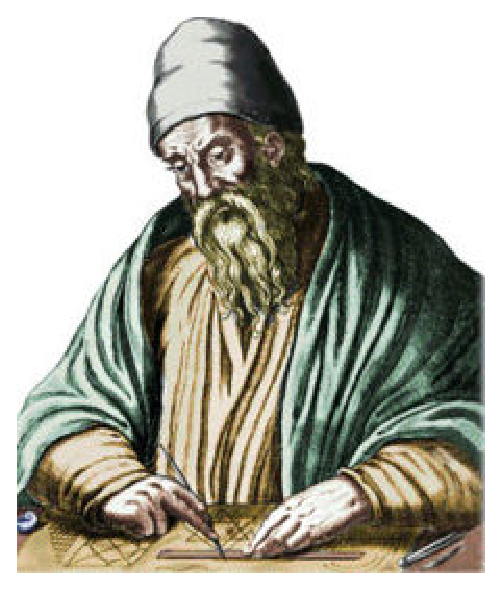
\includegraphics[width=3.5cm]{euclides.eps}
    \captionsetup{singlelinecheck=off,justification=raggedright,margin={1mm,0mm}}
\caption{Euclides}
    \end{minipage}
    \vspace{0pt}
    \hspace{1mm}
    \begin{minipage}[t]{.62\textwidth}
    En el Cap�tulo 1 nos ocupamos  del descubrimiento de las \hyperlink{magnitudes}{cantidades inconmensurables}, esto es, razones de segmentos que no admiten una unidad de medida com�n. El hallazgo de lo que nosotros llamamos ``n�meros irracionales'', como $\sqrt{2}$, no tiene ning�n significado aritm�tico para los griegos; su significado era geom�trico: no puedes medir la diagonal de un cuadrado con su lado.
    \href{http://divulgamat.ehu.es/weborriak/historia/mateospetsuak/Euclides.asp}{Euclides}, el matem�tico m�s famoso de la Escuela de Alejandr�a, en el Libro X de los \emph{Elementos} (300 a.C.), clasifica las magnitudes inconmensurables en los tipos siguientes (uso, claro est�, la notaci�n actual):
\end{minipage}
  \end{figure}

\vspace*{-2mm}\centerline{$\displaystyle{a\pm\sqrt{b},\quad\sqrt{a}\pm\sqrt{b},\quad\sqrt{a\pm\sqrt{b}},\quad\sqrt{\sqrt{a}\pm\sqrt{b}}}$}

Donde se entiende que $a$ y $b$ son racionales.

La existencia de segmentos inconmensurables era un serio problema para el desarrollo de la geometr�a pues, como dichos segmentos no pueden compararse, no se sab�a c�mo interpretar su proporci�n. Por ejemplo, un resultado, sin duda conocido por los pitag�ricos, afirma que \emph{las �reas de dos tri�ngulos con igual altura est�n en la misma proporci�n que sus bases}. �Qu� sentido tiene esta afirmaci�n si las bases no son segmentos conmensurables? El problema est� en que no hab�a una forma de comparar proporciones entre magnitudes inconmensurables. Un matem�tico, \href{http://divulgamat.ehu.es/weborriak/historia/MateOspetsuak/Inprimaketak/Eudoxo.asp}{Eudoxo de Cnido} (\emph{c.}\,400 - 347 a.C.), propuso una teor�a axiom�tica de las magnitudes inconmensurables, que est� recogida en el Libro V de los \emph{Elementos}, en la que destacan los siguientes puntos.

\noindent \textbf{E1} \hypertarget{propiedadarquimediana}{(\emph{Propiedad arquimediana})} Dadas dos magnitudes  siempre hay un m�ltiplo de una de ellas que excede a la otra. Es decir, si es $0<a<b$ hay alg�n \nN\ tal que $na>b$.

\noindent \textbf{E2} (\emph{Criterio de igualdad}) Las proporciones $a:b$ y $c:d$ son iguales si cualesquiera sean los enteros positivos $m$, $n$ se tiene que
\begin{equation}\label{eudoxo}
ma<nb \Longrightarrow mc<nd,\quad ma=nb\Longrightarrow mc=nd,\quad ma>nb\Longrightarrow mc>nd
\end{equation}
Volveremos a considerar m�s adelante este elaborado criterio de igualdad que, desde luego, no aclaraba nada sobre la naturaleza de las cantidades irracionales y pon�a de manifiesto la dificultad de reducir a la aritm�tica el estudio de las mismas.

La carencia de una teor�a aritm�tica satisfactoria de las cantidades inconmensurables, hizo que los matem�ticos griegos consideraran la Geometr�a como una ciencia m�s general que la Aritm�tica, y dedicaran sus esfuerzos al estudio de la primera en detrimento de la �ltima. La consecuencia fue que durante casi 2000 a�os, en Europa, casi todo razonamiento matem�tico riguroso se expres� en lenguaje geom�trico.

Quiz�s el �nico matem�tico griego, despu�s de los pitag�ricos, que no hizo Geometr�a sino Aritm�tica fue Diofanto de Alejandr�a (c.\,214 - 298). En su obra llamada \emph{Aritm�tica}, de la que se han conservado seis libros de un total de trece, resuelve diversos tipos de ecuaciones algebraicas admitiendo como soluciones n�meros enteros o n�meros fraccionarios positivos, los cuales son considerados por Diofanto como aut�nticos n�meros y no solamente como proporciones. Otra innovaci�n de Diofanto fue la invenci�n de una notaci�n ``sincopada'' que constituye el primer ejemplo de simbolismo matem�tico.

\subsection{De la antigua Grecia a la invenci�n del C�lculo}
Es sabido que la civilizaci�n Romana, tan excelente en tantos aspectos, no destac� en el estudio de las ciencias puras y, en particular, de las matem�ticas. La prueba de ello es que no hay ning�n matem�tico Romano digno de menci�n. No obstante, el sistema de numeraci�n Romano se impuso extendi�ndose por todo el Imperio.

Con el triunfo del Cristianismo a finales del siglo IV y la ca�da del Imperio Romano de Occidente en el a�o 476, se inicia una larga era de oscurantismo en Europa. La fe y los dogmas no son demostrables l�gicamente; absurdas disputas teol�gicas ocupan el lugar de los estudios de la Naturaleza y la Biblia es la fuente de todo conocimiento. Seg�n San Agust�n ``las palabras de las Escrituras tienen m�s autoridad que toda la inteligencia humana''. El racionalismo cient�fico es sospechoso de paganismo. Entonces\dots �Para qu� pensar?

A diferencia que en Grecia, en la India se hab�a desarrollado principalmente la Aritm�tica y se conoc�a el sistema de numeraci�n posicional decimal desde el siglo VI. La primera vez que el cero es tratado como un n�mero de pleno derecho es en la obra \emph{Brahmasphutasiddhanta} del matem�tico y astr�nomo indio \href{http://en.wikipedia.org/wiki/Brahmagupta}{Brahmagupta} (598 - 670). Esta obra tambi�n conten�a el principio de la numeraci�n decimal posicional y los m�todos de c�lculo del �lgebra india. En ella se tratan los n�meros negativos en t�rminos muy parecidos a los actuales.



 \begin{figure}[ht]
 \centering
     \begin{minipage}[t]{.35\textwidth}
     \vspace{0pt}
     \flushleft
      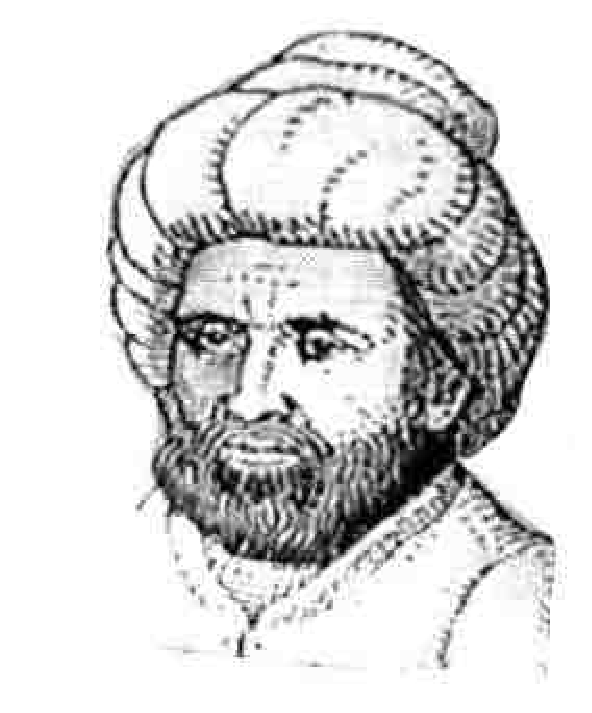
\includegraphics[width=3.5cm]{alkwarizmi.eps}
      \captionsetup{singlelinecheck=off,justification=raggedright,margin={1mm,0mm}}
\caption{al-Jwarizmi}
    \end{minipage}
    \begin{minipage}[t]{.63\textwidth}
    \rule{4mm}{0mm}La herencia matem�tica griega pasa a los �rabes. La cultura �rabe tiene una �poca de esplendor en los siglos VIII - XII. Al-Mamun (c.\,786 - 833), sexto califa de la dinast�a Abasida, fund� en Bagdad la Casa de la Sabidur�a, una especie de academia con una biblioteca y un observatorio. All� se tradujeron las obras de los matem�ticos y fil�sofos griegos y tuvieron conocimiento de las matem�ticas indias.
   \newline\rule{0mm}{5mm} \rule{4mm}{0mm} El m�s conocido matem�tico de la Escuela de Bagdad fue Muhammad ibn-Musa al-Jwarizmi de quien ya hemos hablado en el Cap�tulo 2. En su obra \emph{Libro de la Adici�n y la Sustracci�n seg�n el c�lculo de los hind�es} se describe el sistema decimal posicional y se dan m�todos para realizar c�lculos aritm�ticos con dicho sistema.
     \end{minipage}
  \end{figure}\vspace{-4mm}
 \begin{figure}[ht]
 \centering
     \begin{minipage}[t]{.35\textwidth}
     \vspace{-3cm}
     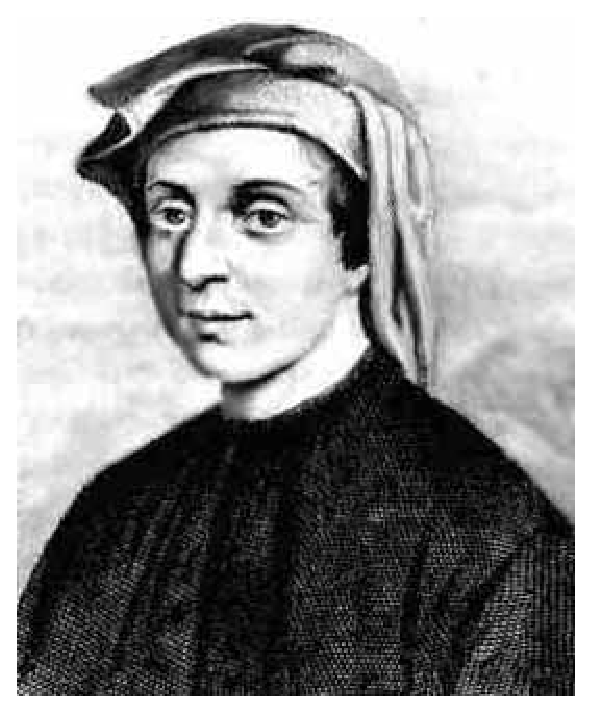
\includegraphics[width=3.5cm]{fibonacci.eps}
      \captionsetup{singlelinecheck=off,justification=raggedright,margin={1mm,0mm}}
\caption{Fibonacci}
    \end{minipage}
    \begin{minipage}{.63\textwidth}
     \rule{4mm}{0mm}\rule{0mm}{5mm}
     \href{http://divulgamat.ehu.es/weborriak/Historia/MateOspetsuak/LeonardoPisa.asp}{ Leonardo de Pisa} (c. 1170 - 1250), m�s conocido como Fibonacci, aprendi� en sus viajes por los pa�ses �rabes del Mediterr�neo a usar los m�todos de al-Jwarizmi. Al regresar a Italia, public� en 1202 el \emph{Liber abaci}, obra que contribuy� a extender el sistema de numeraci�n indo-�rabe en Occidente. Estudiando las soluciones de una ecuaci�n de tercer grado, Fibonacci prob� que hab�a n�meros irracionales diferentes de los considerados por Euclides. En consecuencia, las t�cnicas del �lgebra geom�trica griega no permit�an construir todas las cantidades inconmensurables.
     \end{minipage}
  \end{figure}%\vspace*{-8mm}

\noindent  Fibonacci dio tambi�n una interpretaci�n de los n�meros negativos como p�rdidas o deudas, que tuvo bastante buena acogida. Pero todav�a deber� pasar mucho tiempo para que los n�meros negativos y el cero sean totalmente aceptados como n�meros.

En este apresurado repaso que estamos dando a la historia de los n�meros, debemos avanzar ahora casi trescientos a�os para llegar a la siguiente etapa protagonizada por los matem�ticos italianos del Renacimiento \href{http://www-groups.dcs.st-and.ac.uk/~history/Biographies/Tartaglia.html}{Niccol� Tartaglia} (\emph{c.}\,1500 - 1557), \href{http://es.wikipedia.org/wiki/Cardano}{Gerolamo Cardano} (1501 - 1576), \href{http://www-groups.dcs.st-and.ac.uk/~history/Biographies/Bombelli.html}{Rafael Bombelli} (1526 - 1572) y \href{http://www-groups.dcs.st-and.ac.uk/~history/Biographies/Ferrari.html}{Ludovico Ferrari} (1522 - 1565). Los dos primeros resolvieron la ecuaci�n general de tercer grado de la cual solamente se conoc�an las soluciones en algunos casos particulares. En la resoluci�n de la c�bica, Cardano tuvo en cuenta las\linebreak

   \begin{figure}[ht]
 \centering
     \begin{minipage}[t]{.35\textwidth}
     \vspace*{-2.7cm}
     %\flushleft
      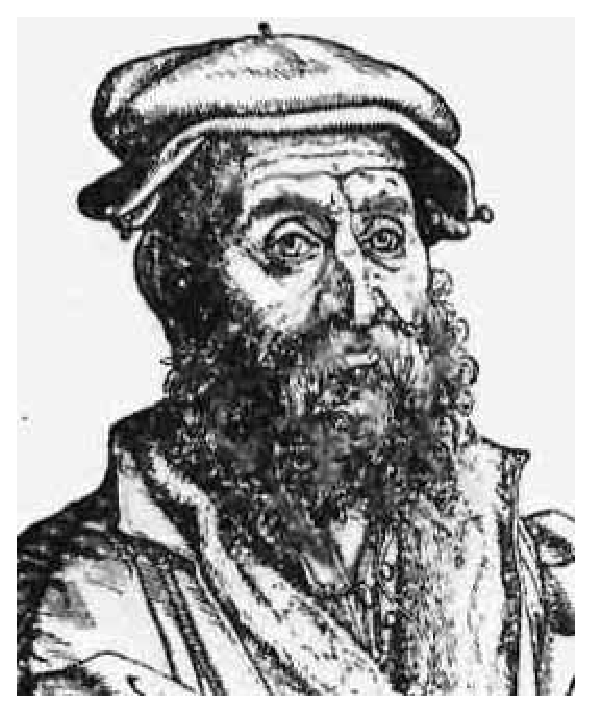
\includegraphics[width=3.5cm]{tartaglia.eps}
      \captionsetup{singlelinecheck=off,justification=raggedright,margin={1mm,0mm}}
\caption{Tartaglia}
    \end{minipage}
    \begin{minipage}{.63\textwidth}
   \vspace*{-5mm} soluciones negativas aunque las llam� ``ficticias'', y comprob� que la c�bica pod�a tener tres soluciones. As� mismo, Cardano reconoci� por primera vez la existencia de lo que ahora llamamos n�meros complejos (a los que Napier llam� ``los fantasmas de los n�meros reales'') aunque no los acept� como posibles soluciones. Por su parte, Bombelli fue el primero en especificar las reglas para sumar y multiplicar n�meros complejos. Usando dichas reglas, prob� que pod�an obtenerse soluciones reales correctas para la c�bica, incluso cuando la f�rmula de Tartaglia -- Cardano requer�a el c�lculo de ra�ces de n�meros negativos.
     \end{minipage}
  \end{figure}\vspace*{-3mm}
De esta �poca es tambi�n un op�sculo \emph{De Thiende} (1585) (``El D�cimo'') -- 36 p�ginas -- de \href{http://divulgamat.ehu.es/weborriak/historia/MateOspetsuak/Stevin.asp}{Simon Stevin} (1548 - 1620), ingeniero y matem�tico nacido en Brujas, en el que se introducen las fracciones decimales y se explica su uso en las operaciones aritm�ticas. As� mismo, en su obra \emph{L'Arithmetique} (1585) escribi� que ``no hay n�meros inexplicables, irregulares, irracionales, surds\footnote{La palabra griega ``alogos'', $\alpha\lambda o\gamma o\varsigma$, usada por los griegos para designar a los n�meros irracionales, tambi�n significa ``sin discurso'' y los �rabes la tradujeron por \emph{asamm}, ``sordo'' o ``mudo'', que fue traducida al lat�n por \emph{surdus}.} o absurdos'', indicando con esto que todos los n�meros deb�an ser tratados por igual y no hacer distinciones entre ellos como si fueran de distinta naturaleza. Despu�s de Stevin, la idea de que 1 era un n�mero gan� una amplia aceptaci�n.

A pesar de estos avances, los conceptos de ``n�mero'' y ``cantidad'' de la antig�edad permanecen sin cambios notables hasta el siglo XVII cuando se desarrolla el simbolismo algebraico.

Lo importante del simbolismo algebraico, no es tanto el uso de los s�mbolos por s� mismos, sino la elaboraci�n de reglas formales para realizar operaciones de forma simb�lica. Por ejemplo, $a^2$ puede entenderse como una forma simplificada de escribir ``el �rea del cuadrado de lado $a$''. Eso es muy distinto de escribir $(a+b)^2=a^2+2ab+b^2$. Esto �ltimo ya es una manipulaci�n simb�lica abstracta en la que las letras $a$, $b$ no son m�s que s�mbolos sin una naturaleza concreta.

\href{http://es.wikipedia.org/wiki/Fran\%C3\%A7ois_Vi\%C3\%A8te}{Fran\c{c}ois Vi�te} en su \emph{In artem analyticem isagoge} (1591) expone una ``logistica speciosa'' (\emph{specis}: s�mbolo), o arte de calcular con s�mbolos, que fue un paso decisivo para el desarrollo del concepto de cantidad abstracta. No obstante, Vi�te consideraba que solamente las cantidades homog�neas pod�an compararse entre s�. Para entender esto debes tener en cuenta que, desde la antig�edad, el producto de dos cantidades, por ejemplo $ab$, representaba el �rea de un rect�ngulo de lados $a$ y $b$. De la misma forma, $abc$ representaba el volumen de un ortoedro. Una expresi�n como $ab+c$ no ten�a significado porque no se pod�a sumar una longitud y un �rea: no eran cantidades homog�neas.

 \begin{figure}[ht]
 \centering
     \begin{minipage}{.275\linewidth}
     %\medskip
     \flushleft
      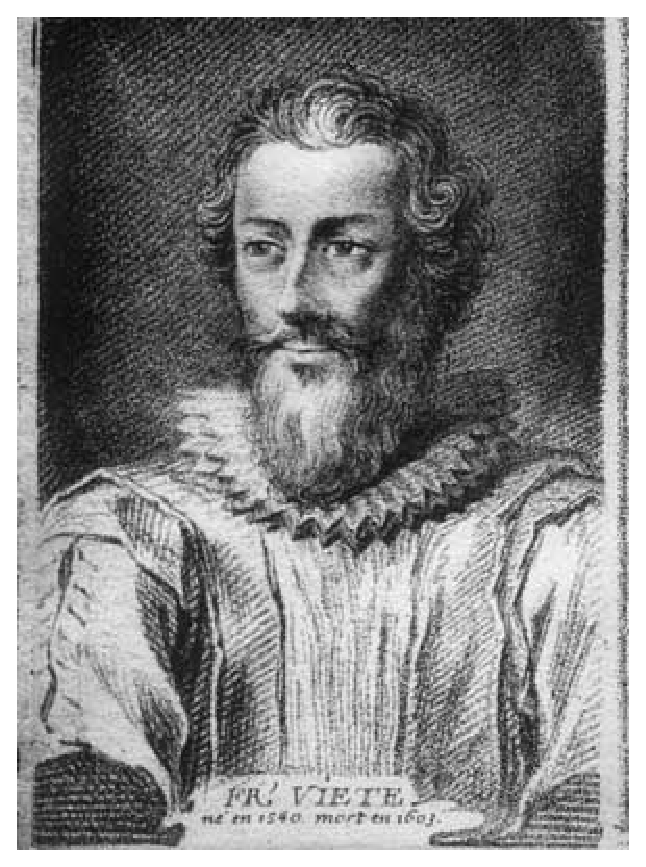
\includegraphics[width=3.5cm]{viete.eps}
      \captionsetup{singlelinecheck=off,justification=raggedright,margin={3mm,0mm}}
\caption{Vi�te}
    \end{minipage}
    \begin{minipage}{.275\linewidth}
      %\medskip
     \centering
      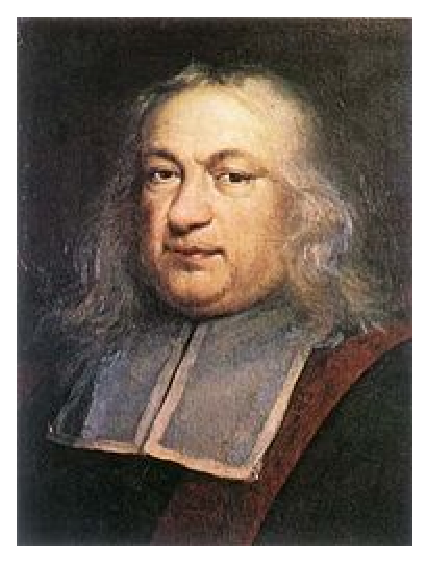
\includegraphics[width=3.5cm]{fermat.eps}
      \captionsetup{singlelinecheck=off,justification=raggedright,margin={5mm,0mm}}
\caption{Fermat}
\end{minipage}
\begin{minipage}{.275\linewidth}
      %\medskip
     \flushright
      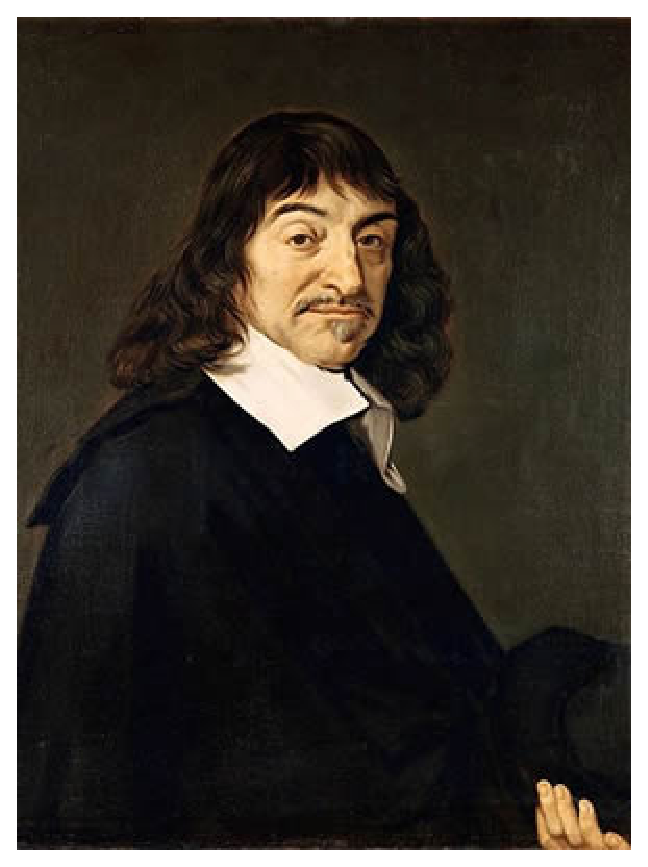
\includegraphics[width=3.5cm]{descartes.eps}
      \captionsetup{singlelinecheck=off,justification=raggedright,margin={6mm,0mm}}
\caption{Descartes}
\end{minipage}
  \end{figure}

El siguiente paso definitivo fue el invento de la \emph{geometr�a anal�tica} en los a�os 1630 por \href{http://en.wikipedia.org/wiki/Fermat}{Pierre Fermat} y \href{http://es.wikipedia.org/wiki/Ren\%C3\%A9_Descartes}{Ren� Descartes}. La introducci�n de coordenadas y la representaci�n de curvas por medio de ecuaciones supuso un cambio de perspectiva revolucionario. Piensa que, en la Antig�edad, solamente pod�an estudiarse aquellas curvas para las que se conoc�a un m�todo de construcci�n con regla y comp�s. Ahora, por primera vez, los objetos geom�tricos pod�an estudiarse por medio del simbolismo algebraico, cuando hasta entonces lo usual hab�a sido que el simbolismo algebraico fuera un p�lido reflejo de relaciones geom�tricas.

Una importante creaci�n de Descartes fue el desarrollo de un ``�lgebra de segmentos''. Para ello, tomando como unidad un segmento $u$, construy� un segmento (cantidad) $c$ que verificaba la proporci�n $u:a = b:c$. Dicho segmento $c$ representaba el producto de los dos segmentos (cantidades) $a$ y $b$. Tambi�n construy� segmentos que se correspond�an con la suma, la diferencia y el cociente de segmentos. De esta manera, cualquier operaci�n con cantidades se corresponde con un segmento, lo que hace que todas las cantidades sean homog�neas. Una expresi�n como $ab+c$ ya es correcta porque representa un segmento de l�nea. Esta homogeneizaci�n de todas las cantidades conduce al concepto de \emph{cantidad abstracta} desconocido en la antig�edad.

Por esta �poca ya tambi�n los n�meros eran objetos abstractos del pensamiento. Es decir, ya no eran simplemente un atributo del grupo al que contaban sino que se hab�an convertido en entidades aut�nomas.

Descartes introdujo el t�rmino ``imaginario'' para referirse a aquellas soluciones de una ecuaci�n polin�mica que solamente est�n en ``nuestra imaginaci�n''. Como era costumbre, llamaba ``soluciones falsas'' a las soluciones negativas. Las ``ra�ces verdaderas'' eran las positivas.

A estos progresos en matem�ticas hay que agregar los realizados en astronom�a y en mec�nica por \href{http://es.wikipedia.org/wiki/Cop\%C3\%A9rnico}{Cop�rnico} (1473-1543), \href{http://es.wikipedia.org/wiki/Kepler}{Kepler} (1571-1630) y \href{http://es.wikipedia.org/wiki/Galileo}{Galileo}(1564-1642). Todos ellos se apoyan en m�todos experimentales y emp�ricos cuantitativos para formular sus resultados como Leyes de la Naturaleza de contenido matem�tico.

Al mismo tiempo, a lo largo de los dos primeros tercios del siglo XVII, se van desarrollando una gran variedad de ``m�todos infinitesimales'', cuyos precedentes cl�sicos estaban en Eudoxo y Arqu�medes, para resolver multitud de problemas de tipo geom�trico y anal�tico, como c�lculo de tangentes a curvas, c�lculo de �reas y de valores m�ximos. Los trabajos de \href{http://www.unex.es/~fan/cuantica/mc\%2010/Web/Tales/cava.html}{Cavalieri} (1598 - 1647) , \href{http://es.wikipedia.org/wiki/John_Wallis}{Wallis} (1616 - 1703) y \href{http://en.wikipedia.org/wiki/Isaac_Barrow}{Barrow} (1630 - 1677) entre otros muchos, establecieron las bases sobre las que dos grandes genios, \href{http://en.wikipedia.org/wiki/Isaac_Newton}{Newton} (1643 - 1727) y \href{http://en.wikipedia.org/wiki/Leibniz}{Leibniz} (1646 - 1716) desarrollaron el C�lculo Infinitesimal. M�s adelante veremos con alg�n detalle todo este proceso, pues ahora quiero considerar solamente aquellos aspectos del mismo relacionados con las ideas de n�mero y de cantidad.

El C�lculo Infinitesimal son las matem�ticas del cambio y del movimiento. Las ideas de magnitud variable y de dependencia entre magnitudes son fundamentales en estas nuevas matem�ticas. Surge as� el concepto de ``variable'' que se forma a partir de la idea de cantidad abstracta. En el libro de L'H�pital \emph{Analyse des infiniment petits, pour l'intelligence des lignes courbes} (1696) se lee:
\begin{quote}
\emph{Se llaman cantidades variables aquellas que aumentan o disminuyen continuamente, y por contraste cantidades constantes aquellas que permanecen igual mientras las otras cambian.}
\end{quote}
Los matem�ticos de los siglos XVII y XVIII usan el t�rmino ``cantidad'' para referirse a cantidades generales abstractas, as� como a cantidades geom�tricas concretas, pero siempre se consideran dichas cantidades como continuas. La noci�n de cantidad continua no se discute, se trataba de un concepto basado en la realidad f�sica. Seg�n Leibniz ``Natura non facit saltus''.

La idea de cantidad es m�s general que la idea de n�mero. Un segmento de l�nea, por ejemplo, representa una cantidad, pero �l mismo no se reduce a n�meros. La idea de n�mero como elemento de un conjunto no existe en el siglo XVIII. Por la misma raz�n, un segmento no puede ``separarse'' de sus extremos y siempre los incluye. Los n�meros eran interpretados como medidas. En \emph{Arithmetica universalis} (1707) Newton escribe:
\begin{quote}
\emph{Por \emph{n�mero} entendemos no tanto una multitud de cantidades, como la raz�n abstracta de cualquier cantidad a otra cantidad de la misma clase que tomamos por unidad. Un entero es lo que es medido por la unidad, una fracci�n, aquello a lo que una parte subm�ltiplo de la unidad mide, y un surd, aquello que es inconmensurable con la unidad.}
\end{quote}
Esta interpretaci�n de los n�meros se corresponde con la consideraci�n de las Matem�ticas en los siglos XVII y XVIII como una Ciencia de la Naturaleza y, en consecuencia, los objetos matem�ticos deben estar vinculados, directa o indirectamente, con la realidad f�sica. Por ello, solamente se consideran como ``verdaderos n�meros'' los que representan el resultado de una medida: los enteros y los racionales positivos. Los dem�s n�meros (negativos, el 0 y los imaginarios) son necesarios y �tiles para los c�lculos, pero no son considerados ``verdaderos n�meros'' son ``ficticios''.

Los n�meros irracionales positivos, aunque no son n�meros en sentido estricto, tampoco son propiamente ``ficticios'', porque pueden representarse por un segmento y sirven para medir cantidades geom�tricamente especificadas. Los racionales e irracionales positivos son llamados ``n�meros reales'' en oposici�n a los n�meros imaginarios.

Los n�meros empiezan a considerarse como entidades simb�licas sobre las que se opera con unas reglas establecidas (pero que no pueden ser libremente definidas). Por ejemplo, seg�n Euler, $\sqrt{12}$ es un n�mero que multiplicado por s� mismo es igual a $12$, y esto es una definici�n simb�lica de $\sqrt{12}$.

El desarrollo inicial del C�lculo, en el �ltimo tercio del siglo XVII, se basa en ideas vagas e imprecisas como ``cantidad evanescente'', ``raz�n �ltima'' o ``infinitamente peque�o''. El uso de los ``infinit�simos'', considerados como cantidades que, sin ser nulas, son m�s peque�as que cualquier cantidad positiva imaginable, es caracter�stico de las t�cnicas del C�lculo.

Despu�s de la invenci�n del C�lculo el objetivo era usarlo para descubrir nuevos resultados. Al principio, nadie se preocup� mucho por la correcci�n matem�tica de los procedimientos empleados. La confianza en dichas t�cnicas descansaba en su extraordinaria eficacia para resolver multitud de problemas. Sin embargo, a finales del siglo XVIII, el uso continuado de los infinit�simos, que nadie sab�a explicar, unido a la incomprensi�n que se ten�a de los n�meros irracionales y de los procesos de convergencia, propiciaron estudios cr�ticos de los conceptos b�sicos del C�lculo, que acabaron llevando a una nueva formulaci�n de los mismos mucho m�s formal y rigurosa, seg�n los criterios actuales, pero tambi�n mucho menos intuitiva.

\subsection{Infinit�simos y el continuo num�rico}
Est�s leyendo \emph{ahora mismo} estas palabras. Tienes un sentido preciso del ``ahora'', al igual que del ``pasado'' y del ``futuro''. Tenemos una percepci�n muy clara del ``flujo del tiempo''. Percibimos el tiempo como un continuo: lo que separa dos instantes de tiempo es \dots tiempo. Dado un peque�o intervalo de tiempo, digamos un segundo, siempre podemos concebir otro intervalo m�s peque�o todav�a, medio segundo o una cienbillon�sima parte de un segundo. �Has pensado alguna vez hasta d�nde es posible \emph{dividir el tiempo}? Si aceptamos que el ``instante'' es lo que no tiene duraci�n, parece dif�cil aceptar que el tiempo est� formado por instantes. �Debemos considerar entonces que hay una \emph{unidad m�nima} de tiempo, todo lo peque�a que queramos, pero que no se reduce a un instante? Estar�s de acuerdo en que esa unidad m�nima de tiempo ser�a algo as� como una unidad de tiempo ``infinitesimal''. �Cu�ntas unidades infinitesimales de tiempo caben en un minuto? �Un n�mero finito? �Una cantidad infinita?

En el p�rrafo anterior podemos cambiar la palabra ``tiempo'' por ``espacio'' e ``instante'' por ``punto'' y llegaremos a los problemas derivados de la ``infinita divisibilidad'' del espacio. Tiempo y espacio son ejemplos de ``continuo''.  Una entidad continua, un \emph{continuo}, es lo que no est� roto ni separado ni tiene huecos, lo que puede ser indefinidamente dividido sin que pierda su naturaleza. Por ejemplo, un volumen de l�quido, un segmento, un movimiento o, los ejemplos m�s inmediatos, el espacio y el tiempo.

Lo que relaciona espacio y tiempo es el movimiento. El C�lculo es la matem�tica del movimiento, del cambio continuo. El C�lculo se apoya en la geometr�a anal�tica de Descartes y Fermat y en la Aritm�tica. La Geometr�a se ocupa de cantidades continuas; la Aritm�tica de lo discreto. El C�lculo es la s�ntesis de lo ``discreto'' y lo ``continuo''. Los ``infinit�simos'', las cantidades infinitesimales, son el puente entre lo discreto y lo continuo.

Los procedimientos del C�lculo, l�mites, convergencia, continuidad, pueden describirse como matem�ticas del \emph{continuo num�rico}. La expresi�n ``continuo num�rico'' puede parecer un ox�moron, esto es, una combinaci�n de dos palabras con significados opuestos y, en cierto sentido, es as�. Los n�meros sirven para contar grupos de cosas de igual naturaleza; por ejemplo �rboles, o lo que quiera que sea, pero cada una de ellas con su propia individualidad, separadas entre s�, cosas que no tiene sentido dividir porque al hacerlo pierden su naturaleza. Todo esto se resume diciendo que los n�meros tienen un car�cter \emph{discreto}. Los n�meros siempre fueron considerados como lo opuesto del continuo.

La oposici�n continuo  -- discreto ha ocupado a los fil�sofos desde hace 2500 a�os y tiene como primeros representantes respectivos a \href{http://es.wikipedia.org/wiki/Parm\%C3\%A9nides_de_Elea}{Parm�nides} (\emph{c.}\,510 - 450 a.C.) y a \href{http://es.wikipedia.org/wiki/Dem\%C3\%B3crito}{Dem�crito} (\emph{c.}\,460 - 370 a.C.).

Parm�nides, el fil�sofo m�s famoso de la Escuela Ele�tica, afirma en su hermoso poema \emph{Sobre la Naturaleza}, que lo que Es, el Ser, es uno, ing�nito, homog�neo, continuo, indivisible e inmutable. Este concepto del Ser excluye toda posibilidad de nueva generaci�n de seres o sustancias y, por tanto, el cambio y el movimiento son mera ilusi�n, porque ambos presuponen que lo que no es pueda llegar a ser.

Dem�crito es el representante m�s conocido de la Escuela Atomista cuyo materialismo se opone al idealismo de la Escuela Ele�tica. Dem�crito mantiene que el universo est� compuesto de peque�os corp�sculos invisibles, los ``�tomos'',  que pueden poseer diferentes formas y extensiones y que por movimientos y combinaciones diversas en el vac�o engendran la totalidad de lo existente.

\href{http://es.wikipedia.org/wiki/Zen\%C3\%B3n_de_Elea}{Zen�n de Elea}, disc�pulo de Parm�nides, es famoso por sus \emph{apor�as}, en las que trata de probar que tanto si el espacio o el tiempo son infinitamente divisibles, como si no lo son, el movimiento no existe o es imposible. Las apor�as de Zen�n son un extraordinario desaf�o, al que fil�sofos y matem�ticos han dado diversas respuestas, sin que a�n hoy se tenga conciencia clara de haberlas podido explicar de forma totalmente convincente.

Seg�n Arist�teles, los atomistas preguntaban, en el supuesto de que una magnitud sea infinitamente divisible, qu� es lo que quedaba de ella despu�s de haberla sometido a un proceso de divisi�n exhaustivo. Y dec�an, si queda algo como polvo, es porque todav�a no se ha completado el proceso de divisi�n, y si lo que queda son puntos o algo sin extensi�n, �c�mo es posible recomponer una magnitud extensa con algo que no tiene extensi�n? Seg�n ellos, la respuesta eran los �tomos. La palabra griega ``�tomos'' significa ``lo que no puede dividirse'', por tanto, la Escuela Atomista negaba la infinita divisibilidad de la materia y afirmaba que cualquier magnitud contiene elementos indivisibles.

De la oposici�n continuo -- discreto siguieron ocup�ndose los fil�sofos de la Antig�edad,  \href{http://es.wikipedia.org/wiki/Platon}{Plat�n} (\emph{c.}\,427 - 347 a.C.), \href{http://es.wikipedia.org/wiki/Aristoteles}{Arist�teles} (384 - 322a.C.), \href{http://es.wikipedia.org/wiki/Epicuro}{Epicuro} (341 - 270 a.C.); y de la Edad Media \href{http://es.wikipedia.org/wiki/Duns_Scoto}{Duns Scoto} (\emph{c.}\,1266 - 1308), \href{http://es.wikipedia.org/wiki/Guillermo_de_Ockham}{Guillermo de Ockham} (\emph{c.}\,1280 - 1349), \href{http://es.wikipedia.org/wiki/Nicolas_de_Cusa}{Nicol�s de Cusa} (1401 - 1464), entre otros. �ste �ltimo, en una supuesta demostraci�n de la cuadratura del c�rculo, consider� una circunferencia como un pol�gono regular de infinitos lados. La idea de considerar que una curva est� formado por infinitos segmentos infinitesimales de l�nea recta  fue usada, entre otros, por Kepler, Galileo y Leibniz y est� recogida en el libro de Guillaume de L'H�pital \emph{Analyse des Infiniment Petits pour l'Intelligence des Lignes Courbes} (1696) al cual ya nos hemos referido anteriormente.

A finales del siglo XVII, con el invento del C�lculo, resurgi� la oposici�n entre lo continuo y lo discreto, esta vez centrada en el concepto de cantidad infinitesimal. Algunos consideraban los infinit�simos como algo real, infinitamente peque�o, parecido a los �tomos de Dem�crito, salvo que ahora su n�mero era infinito. La integraci�n se consideraba como una suma infinita de estos infinit�simos. Una diferencial de una cantidad variable era un incremento infinitesimal de dicha variable, y un cociente o una raz�n de diferenciales ``en el momento en que se anulan'', lo que Newton llamaba \emph{cantidades evanescentes}, era lo que ahora llamamos una derivada, y Newton llamaba una \emph{fluxi�n}.

El uso de los infinit�simos en el C�lculo demostraba ser muy eficaz y, aunque a algunos, como al mismo Newton, les hubiera gustado evitarlo, lo cierto es que no se sab�a bien c�mo hacerlo. Lo peor de todo, no es que el mero concepto de infinit�simo sea de por s� dif�cilmente sostenible, sino la forma en que los infinit�simos se manejaban en los c�lculos. Podemos destacar dos caracter�sticas.
\begin{itemize}
\item[$\bullet$] Con los infinit�simos pod�a operarse como con cantidades finitas no nulas y, en particular, pod�a dividirse por ellos.
\item[$\bullet$] Los infinit�simos pod�an ser tratados como cantidades nulas. As�, si $x$ es una cantidad positiva y $o$ un infinit�simo, entonces $\,x+o=x$.
\end{itemize}
Dependiendo del tipo de c�lculo eran tratados de una forma u otra. Adem�s, hab�a infinit�simos de primer orden despreciables frente a cantidades finitas; de segundo orden que eran despreciables frente a los de primer orden, y as� sucesivamente. Para acabar de empeorar las cosas, los infinit�simos no respetaban la \hyperlink{propiedadarquimediana}{propiedad arquimediana}, pues el producto de cualquier cantidad finita por un infinit�simo segu�a siendo un infinit�simo.
\begin{ejemplo}
Un ejemplo t�pico es el c�lculo de la diferencial de un producto de dos cantidades $x$ e $y$. Se razonaba como sigue. Cuando $x$ cambia a $x+\df{x}$, $y$ cambia a $y+\df{y}$, por lo que $xy$ se transforma en $$(x+\df{x})(y+\df{y})=xy+x\df{y}+y\df{x}+\df{x}\!\df{y}$$
por lo que la diferencial de $xy$ es $x\df{y}+y\df{x}+\df{x}\!\df{y}$, pero como $\df{x}\!\df{y}$ es una cantidad infinitamente peque�a con respecto a los otros t�rminos, se sigue que la diferencial de $xy$ es $x\df{y}+y\df{x}$.
\end{ejemplo}
\begin{ejemplo}\label{derivadainfinitesimal}
Veamos otro ejemplo t�pico. Consideremos dos cantidades $x$, $y$ relacionadas por $y-x^3=0$. Cuando $x$ cambia a $x+\df{x}$, $y$ cambia a $y+\df{y}$, por lo que
$$
0=y+\df{y}-(x+\df{x}\!)^3=y+\df{y}-x^3-3x^2\df{x}-3x(\df{x}\!)^2-(\df{x}\!)^3
$$
Teniendo en cuenta que $y-x^3=0$, deducimos:
$$
\df{y}=3x^2\df{x}+3x(\df{x}\!)^2+(\df{x}\!)^3
$$
Dividiendo por $\df{x}$ la igualdad obtenida resulta:
$$
\dfrac{\df{y}}{\df{x}}=3x^2+3x\df{x}+(\df{x}\!)^2
$$
Y como $3x\df{x}+(\df{x}\!)^2$ es infinitamente peque�o respecto de $3x^2$, concluimos que $\dfrac{\df{y}}{\df{x}}=3x^2$.

En lenguaje actual, lo que hemos hecho es calcular la derivada de la funci�n $f(x)=x^3$. Y\dots �el resultado es correcto! A pesar de que hemos dividido por una cantidad que despu�s hemos hecho igual a cero.
\end{ejemplo}
En 1734 el fil�sofo \href{http://es.wikipedia.org/wiki/Bishop_Berkeley}{George Berkeley} (1685 - 1753) public� una obra cuyo t�tulo es \emph{El analista, o discurso dirigido a un matem�tico infiel, donde se examina si el objeto, principios e inferencias del an�lisis moderno est�n formulados de manera m�s clara, o deducidos de manera m�s evidente, que los misterios de la religi�n y las cuestiones de la fe}. En dicha obra Berkeley, que fue obispo anglicano de Cloyne, hace una cr�tica de los fundamentos del C�lculo que tuvo una gran influencia. Afirmaba Berkeley que si se acepta que el C�lculo  puede alcanzar soluciones exactas por medio de razonamientos err�neos, entonces debe admitirse que la fe puede alcanzar la verdad por v�as m�sticas. Es famoso su comentario:
\begin{quote}
\emph{�Qu� son las fluxiones? Las velocidades de incrementos evanescentes. Y �qu� son estos mismos incrementos evanescentes? Ellos no son ni cantidades finitas, ni cantidades infinitamente peque�as, ni siquiera son nada. �No las podr�amos llamar los fantasmas de las cantidades desaparecidas?}
\end{quote}
Los embrollos en que andaban metidos los matem�ticos se reflejan en la novela de Jonathan Swift \emph{Los viajes de Gulliver} (1726) donde aparecen los diminutos enanos de Lilliput y los enormes gigantes de Brobdingnag, y en la narraci�n corta \emph{Micromegas} (1752) de Voltaire.

La realidad es que los matem�ticos del siglo XVIII, y hasta bien entrado el siglo XIX, estaban mucho m�s interesados en desarrollar y aplicar las t�cnicas del C�lculo, que en ocuparse de problemas de fundamentos. Entre los principales matem�ticos de esta �poca hay que citar a \href{http://divulgamat.ehu.es/weborriak/Historia/MateOspetsuak/Euler.asp}{Leonard Euler} (1707 - 1783), \href{http://www-history.mcs.st-andrews.ac.uk/history/Biographies/D'Alembert.html}{Jean d'Alembert} (1717 - 1783), \href{http://www-history.mcs.st-andrews.ac.uk/history/Biographies/Lagrange.html}{Joseph-Louis Lagrange} (1736 - 1813), \href{http://www-history.mcs.st-andrews.ac.uk/history/Biographies/Laplace.html}{Pierre-Simon Laplace} (1749 - 1827), \href{http://www-history.mcs.st-andrews.ac.uk/history/Biographies/Fourier.html}{Joseph Fourier} (1768 - 1830), \href{http://divulgamat.ehu.es/weborriak/Historia/MateOspetsuak/Gauss.asp}{Carl Friedrich Gauss} (1777 - 1855). El esp�ritu de los tiempos, el Siglo de las Luces, queda bien reflejado en la siguiente frase.
\begin{quote}
\emph{Todos los efectos de la naturaleza son tan s�lo las consecuencias matem�ticas de un peque�o n�mero de leyes inmutables.}\hfill{Laplace}
\end{quote}
En el primer tercio del siglo XIX, el ideal de Newton de ``someter los fen�menos de la Naturaleza a las leyes matem�ticas'', pod�a considerarse esencialmente realizado.
\subsection{El triunfo de Pit�goras}
Llegamos as� al siglo XIX que, en cuanto a matem�ticas se refiere, ha sido llamado el Siglo del Rigor. Veamos c�mo se entend�an en los primeros a�os de dicho siglo los conceptos b�sicos del C�lculo.
\begin{itemize}
\item[$\bullet$] Concepto de funci�n. No exist�a tal como lo entendemos en la actualidad. En vez de funciones, se consideraban relaciones entre variables, es decir, ecuaciones. Las correspondencias entre variables se interpretaban en t�rminos geom�tricos. No exist�a la idea del dominio de una variable.
\item[$\bullet$] Concepto de continuidad. El concepto de continuidad puntual no hab�a sido siquiera formulado matem�ticamente. La idea de Euler de funci�n continua, como aquella que est� definida por una �nica expresi�n anal�tica, era todo lo que hab�a.
\item[$\bullet$] Concepto de l�mite. Solamente se ten�an algunas ideas confusas agravadas por el uso de los infinit�simos. Los infinit�simos empezaban a considerarse como variables con l�mite cero.
\item[$\bullet$] Concepto de n�mero. La idea de cantidad abstracta variable, a la que pod�an asignarse valores concretos, no hab�a experimentado cambios notables en casi un siglo. Los n�meros complejos ya eran aceptados, gracias a los trabajos de Euler y, sobre todo, de Gauss, pero segu�a sin tenerse una idea clara de los n�meros irracionales, y prevalec�a una interpretaci�n geom�trica de los mismos.
\end{itemize}
Esta situaci�n iba a cambiar gracias principalmente a los trabajos de \href{http://es.wikipedia.org/wiki/Bernard_Bolzano}{Bernad Bolzano} (1781 - 1848),
\href{http://www-history.mcs.st-andrews.ac.uk/Biographies/Cauchy.html}{Augustin Louis Cauchy} (1789 - 1857) y \href{http://www-history.mcs.st-andrews.ac.uk/Biographies/Weierstrass.html}{Karl Weierstrass} (1815 - 1897) de los que nos ocuparemos al estudiar la formalizaci�n del concepto de l�mite. Ahora quiero detenerme solamente en la evoluci�n de la idea de n�mero real. A los tres matem�ticos citados hay que agregar los nombres de \href{http://divulgamat.ehu.es/weborriak/Historia/MateOspetsuak/Dedekind.asp}{Richard Dedekind} (1831 - 1916) y \href{http://en.wikipedia.org/wiki/Georg_Cantor}{George Cantor} (1845 - 1918), fueron ellos quienes desarrollaron la teor�a de los n�meros reales que hemos estudiado en los Cap�tulos 1 y 4. Es l�gico preguntarse por qu� esto no se hizo antes. Pueden darse varias razones para ello.
\begin{itemize}
\item[$\bullet$] En el siglo XVIII las matem�ticas son consideradas una Ciencia de la Naturaleza. Las teor�as matem�ticas deben reflejar la realidad f�sica. Las matem�ticas son una herramienta para formular y descubrir las Leyes de la Naturaleza. Las teor�as matem�ticas no se inventan, se descubren.
\item[$\bullet$] Los n�meros reales estaban asociados con magnitudes y se interpretaban geom�tricamente. Eran algo dado en la realidad f�sica. A los matem�ticos del siglo XVIII no les pareci� necesario dar una definici�n matem�tica de los mismos.
\item[$\bullet$]  Observa que para precisar un n�mero como $\sqrt{2}$ debes dar todas sus cifras decimales en su orden, es decir, un vector de infinitas componentes. F�jate tambi�n que la condici�n dada por Eudoxo (\ref{eudoxo}) para comparar razones inconmensurables hace intervenir a \emph{todos} los n�meros naturales. Esto no es casual. La idea de n�mero irracional lleva consigo asociada la de infinito. Hasta que no se elaboraron los fundamentos de una teor�a matem�tica del infinito, no pudo desarrollarse una teor�a satisfactoria de los n�meros reales.
\end{itemize}
En el siglo XVIII las definiciones matem�ticas eran descriptivas; no creaban objetos matem�ticos sino que describ�an algo que se supon�a deb�a imitar una realidad externa. Por la misma raz�n, no pod�an inventarse reglas para operar con los objetos matem�ticos. Las reglas hab�a que descubrirlas, pero no pod�an elegirse libremente.  Se consideraba que la Naturaleza impon�a unas normas que las Matem�ticas de alguna manera deb�an imitar, no se era libre para inventar una teor�a matem�tica. La idea de una Matem�tica como juego l�gico formal era algo impensable en el siglo XVIII.

La idea que los matem�ticos ten�an de su Ciencia cambi� de forma radical como consecuencia de la invenci�n en el siglo XIX de las geometr�as no eucl�deas por \href{http://www-history.mcs.st-andrews.ac.uk/Biographies/Bolyai.html}{Janos Bolyai} (1802 - 1860) y \href{http://www-history.mcs.st-andrews.ac.uk/Biographies/Lobachevsky.html}{Nikolai I. Lobachevsky} (1792 - 1856). Qued� claro a partir de entonces que las matem�ticas no son una Ciencia de la Naturaleza, que la definici�n usual de las matem�ticas como la ciencia que estudia la cantidad y la forma es inadecuada, y pas� a considerarse que la matem�tica es la ciencia que obtiene conclusiones l�gicas de sistemas axiom�ticos. Las matem�ticas son, pues, una ciencia puramente deductiva. Una teor�a matem�tica es un conjunto de axiomas que contienen ciertos t�rminos indefinidos, y un sistema de reglas de inferencia l�gica. El papel que juegan las definiciones en una teor�a matem�tica consiste en crear nuevos objetos matem�ticos y precisar su significado en dicha teor�a. Todos los objetos que se estudian en una teor�a matem�tica, o bien son t�rminos indefinidos de dicha teor�a o son objetos creados por medio de definiciones que remiten a los axiomas. En el XVIII los n�meros reales son algo dado y externo que las matem�ticas deben explicar, al final del XIX los n�meros ser�n algo completamente diferente.

La idea de n�mero real es el soporte de otras ideas b�sicas del C�lculo como las de continuidad y l�mite. Los procesos de convergencia dependen de la propiedad de completitud de los n�meros reales. Por todo ello, los matem�ticos eran cada vez m�s conscientes de que los progresos del C�lculo depend�an de un mejor conocimiento de los mismos.
\subsubsection{Cortaduras de Dedekind}
A mediados del siglo XIX no era posible demostrar algunos resultados b�sicos del c�lculo; por ejemplo, que toda funci�n creciente y acotada tiene l�mite, o el teorema del valor intermedio para funciones continuas. Ello se deb�a a que faltaba codificar matem�ticamente una propiedad fundamental de los n�meros reales, la que ahora llamamos \emph{completitud} y entonces se llamaba \emph{propiedad de continuidad}. En 1872 se publicaron dos trabajos, uno de Cantor y otro de Dedekind, en los que, tomando como punto de partida el sistema de los n�meros racionales, cada autor desarrollaba una construcci�n matem�tica de los n�meros reales. Nos vamos a ocupar aqu� del trabajo de Dedekind, titulado \emph{Continuidad y n�meros irracionales}. En dicho trabajo, Dedekind manifiesta su prop�sito de reducir los n�meros reales a la aritm�tica, eliminando as� todo contenido geom�trico en la idea de n�mero real. Para explicar lo que �l hizo vamos a partir de la intuici�n de una recta.
 \begin{figure}[ht]
\begin{center}
     \begin{minipage}[t]{.3\textwidth}
     \vspace{0pt}
     \hspace{2mm}
      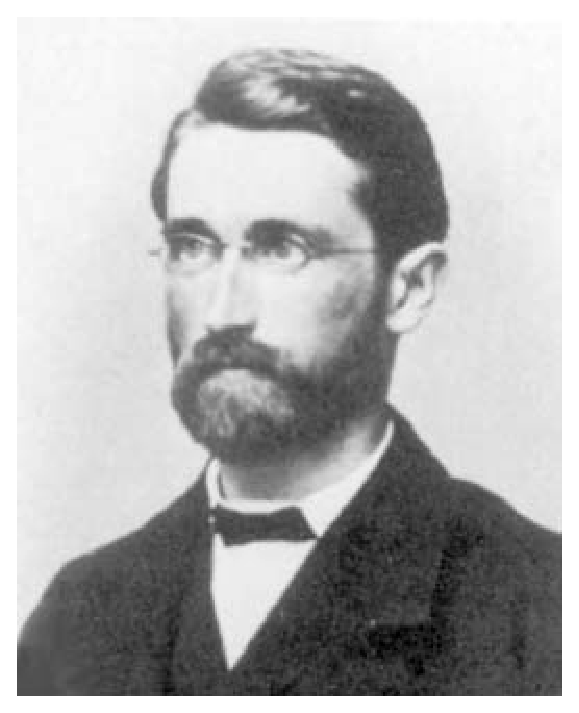
\includegraphics[width=3cm]{dedekind.eps}
      \captionsetup{singlelinecheck=off,justification=raggedright}%,margin={1mm,0mm}
\caption{Dedekind}
    \end{minipage}%
       \begin{minipage}[t]{.7\textwidth}
       \vspace{0pt}
   Una recta es un ejemplo claro de continuidad. Elegido un punto como origen y un segmento como unidad, podemos hacer corresponder a cada n�mero racional un punto de esa recta. Ya hemos visto, al hablar de las magnitudes inconmensurables, que los n�meros racionales no agotan todos los puntos de la recta; cualquier punto que corresponda con un segmento de longitud inconmensurable con la unidad elegida no puede ser representado por un n�mero racional, es decir, en la recta racional hay ``huecos''. Por tanto, los n�meros racionales no son suficientes para describir num�ricamente ``el continuo''. Se pregunta Dedekind:
     \end{minipage}
      \end{center}
  \end{figure}\vspace*{-1.1cm}
\begin{quote}
\emph{�En qu� consiste esta continuidad? Todo depende de la respuesta a esta pregunta, y solamente a trav�s de ella obtendremos una base cient�fica para la investigaci�n de todos los dominios continuos. Con vagas observaciones sobre la uni�n sin rotura de las partes m�s peque�as, obviamente nada se gana; el problema es indicar una caracter�stica precisa de la continuidad que pueda servir como base para deducciones v�lidas. Durante largo tiempo he meditado sobre esto en vano, pero finalmente he encontrado lo que pretend�a.}
\end{quote}
Dedekind se dispone a revelar el secreto, pero como su idea adem�s de ser genial es muy sencilla, previene al lector con esta observaci�n.
\begin{quote}
\emph{Muchos de mis lectores quedar�n grandemente disgustados al saber que por esta vulgar observaci�n se revela el secreto de la continuidad.}
\end{quote}
�Cu�l es esa \emph{vulgar} observaci�n? Vamos a explicarla. Todo punto en una recta $R$ la divide en dos partes disjuntas, la parte $A$, formada por los puntos de la recta que est�n a su izquierda, y la parte $B$, formada por los puntos de la recta que est�n a su derecha. El propio punto podemos incluirlo bien en $A$ o en $B$. Dice Dedekind:
\begin{quote}
\emph{He encontrado la esencia de la continuidad en el rec�proco, es decir, en el siguiente principio:\emph{``Si todos los puntos de la recta se dividen en dos clases tales que todo punto de la primera clase queda a la izquierda de todo punto de la segunda clase, entonces existe un, y s�lo un punto, que produce esta divisi�n de todos los puntos en dos clases, esta escisi�n de la l�nea recta en dos partes.''}}
\end{quote}
Las ideas geniales, que adem�s son sencillas, son doblemente geniales. Igual que el tiempo es continuo porque entre dos instantes de tiempo solamente hay tiempo, la recta es continua porque entre dos puntos de ella solamente hay puntos de la misma recta. Es esta la idea que Dedekind ha sabido expresar matem�ticamente de una forma insuperable. Para entenderla un poco mejor, vamos a considerar el conjunto \Q\ de los n�meros racionales como puntos de una recta en la que hemos elegido un origen y una unidad, la recta racional.
\begin{definicion}
Una \emph{cortadura} de \Q\ es un par $(A,B)$, donde $A$ y $B$ son conjuntos no vac�os de n�meros racionales tales que $\,\Q=A\cup B$, y todo n�mero de $A$ es menor que todo n�mero de $B$ y $A$ no tiene m�ximo.
\end{definicion}
Todo n�mero racional $r\en\Q$ produce una cortadura dada por
$$
A=\set{x\en\Q:x<r},\qquad B=\set{x\en\Q:r\ge x}
$$
Pero en la recta racional hay muchas cortaduras que no est�n producidas por n�meros racionales. En el ejercicio (\ref{cortenoracional}) hemos visto que los conjuntos
$$
A=\{x\en\Q:x\leqslant 0 \ \ {\rm o}\ \ x^{2}<2\},\ \ B=\{x\en\Q:x>0\ \ {\rm y}\ \ x^{2}\geqslant 2\}
$$
definen una cortadura de \Q\ que no est� producida por ning�n n�mero racional. De hecho, si te imaginas la recta racional dentro de la recta real, y tomas un n�mero $\alpha$ que sea irracional, los conjuntos
$$
A=\set{x\en\Q:x<\alpha},\qquad B=\set{x\en\Q:r>\alpha}
$$
Definen una cortadura de \Q\ que no est� producida por ning�n n�mero racional. Es decir, considerando \Q\ dentro de \R, vemos que cada cortadura de \Q\ est� determinada por un punto que puede ser racional o irracional.

Pero claro, \emph{est� prohibido usar la recta real cuando lo que queremos es justamente construirla a partir de} \Q. �De d�nde sacamos los n�meros reales si todo lo que tenemos son los racionales? Esta es la idea genial de Dedekind.
\begin{definicion}
Un n�mero real es una cortadura de \Q.
\end{definicion}
El conjunto de todos los n�meros reales se representa por \R. Observa el papel que desempe�an las definiciones en una teor�a matem�tica: crean nuevos objetos de la teor�a. La definici�n anterior dice lo que es un n�mero real en t�rminos exclusivamente de n�meros racionales. Vuelve ahora a leer la definici�n de Eudoxo (\ref{eudoxo}) para la igualdad de razones inconmensurables. �Lo que dice (\ref{eudoxo}) es que dos razones inconmensurables son iguales si producen una misma cortadura en \Q! Salvo esto, ning�n otro parecido hay entre Dedekind y Eudoxo.

Los n�meros racionales se construyen a partir del conjunto \Z\ de los enteros, y �stos se obtienen f�cilmente a partir de los naturales. Dedekind y \href{http://es.wikipedia.org/wiki/Giuseppe_Peano}{Giuseppe Peano} establecieron una base axiom�tica para el conjunto \N\ de los n�meros naturales. Ya ves, al final, Pit�goras ha regresado: todo es n�mero.

\subsubsection{M�todos axiom�ticos y m�todos constructivos}
Supongo lo que est�s pensando: ``�Vaya definici�n extra�a de n�mero real! Ahora resulta que un n�mero es una cortadura\dots �nada menos que dos conjuntos infinitos de n�meros!''. Vayamos poco a poco.
\begin{itemize}
\item[$\bullet$] Es una definici�n operativa, es decir, permite definir la suma y el producto de n�meros reales, as� como la relaci�n de orden y demostrar las propiedades \textbf{P1} - \textbf{P7} del Cap�tulo 1, y tambi�n la propiedad del supremo \textbf{P8}. Adem�s, todo esto se hace de forma sencilla aunque laboriosa. Si tienes curiosidad, puedes consultar el Cap�tulo 28 de \cite{spivak}.
\item[$\bullet$] Lo importante de la definici�n es que define los n�meros reales solamente usando los n�meros racionales. Es decir, resuelve un problema de \emph{existencia} en sentido matem�tico.
\end{itemize}

Las propiedades o axiomas \textbf{P1} - \textbf{P7} del Cap�tulo 1, junto con la propiedad del supremo \textbf{P8}, definen una estructura que se llama \emph{cuerpo ordenado completo}. Aunque en el Cap�tulo 1 dijimos que no era nuestro prop�sito decir qu� son los n�meros reales, podemos ahora responder a dicha pregunta: \emph{los n�meros reales son el �nico cuerpo ordenado completo}. La demostraci�n de que {\em existe\/} un cuerpo ordenado completo y es {\em �nico\/} es larga, laboriosa y depende de las hip�tesis de partida.

Lo m�s usual es dar por conocidos los n�meros racionales y a partir de ellos {\em construir} \R. Esto puede parecer extra\~no a primera vista, porque si s�lo conocemos los n�meros racionales, �de d�nde van a salir los dem�s? De eso precisamente se ocupan los \emph{m�todos constructivos} (Cantor, Dedekind). Por ejemplo, si partimos de la intuici�n de que con los n�meros reales se pueden representar {\em todos\/} los puntos de una recta, es claro que un n�mero real queda determinado de forma �nica por los n�meros racionales menores que �l. Esta idea conduce a la {\em definici�n} de n�mero real dada por Dedekind.
La definici�n de Cantor es mucho menos intuitiva pues, para Cantor, un n�mero real es una clase de infinitas sucesiones de n�meros racionales que cumplen una cierta propiedad.

Es posible probar, partiendo de estas definiciones, que el conjunto de los
n�meros reales as� definidos puede dotarse de una estructura algebraica y de orden de manera que satisface los axiomas \textbf{P1} - \textbf{P8}. Este proceso es bastante laborioso; adem�s se corre el peligro de centrar la atenci�n en el proceso en s� mismo olvid�ndose de lo que se persigue. Por otra parte, las definiciones de Dedekind o de Cantor no son las �nicas, hay otras definiciones de n�mero real. Pensar�s que esto no es serio. �Qu� est� ocurriendo aqu�? Ocurre, sencillamente, que cualquier definici�n de los n�meros reales a partir de los racionales, esto es, cualquier m�todo constructivo de \R, tiene su raz�n �ltima de ser en el {\em problema de la existencia}: �puede ser construido un cuerpo ordenado completo a partir de los axiomas usuales de la Teor�a de Conjuntos? Pues bien, la respuesta es que s�; adem�s, y esto es fundamental, matem�ticamente, en un sentido preciso, dicho cuerpo {\em es �nico}.

Da igual, por tanto, c�mo se interprete lo que es un n�mero real, lo importante es que de cualquier forma que lo hagamos, los axiomas \textbf{P1} - \textbf{P8} determinan totalmente sus propiedades matem�ticas. Es decir, una vez que sabemos que hay un �nico cuerpo ordenado completo, lo mejor es olvidar cualquier posible interpretaci�n de c�mo sean sus elementos (ning�n matem�tico
cuando considera el n�mero real $\,\sqrt{2}\,$ piensa que $
\sqrt{2}=\{x\en\Q:x<0 \ \ {\rm o}\ \  x^{2}<2\}$) y quedarnos exclusivamente con las propiedades de los mismos. Esto es precisamente lo que se hace con el m�todo axiom�tico que nosotros hemos elegido para presentar \R.
\subsubsection{El regreso de los peque�itos}
Con la reducci�n del continuo a lo discreto, parece que finalmente ha triunfado la Aritm�tica. Pero la historia continua. Por una parte, los n�meros naturales tuvieron un reinado ef�mero, pues fueron esencialmente reducidos a pura l�gica como consecuencia del trabajo pionero de \href{http://es.wikipedia.org/wiki/Frege}{Gottlob Frege}. Por otra parte en  1960, el l�gico \href{http://www-history.mcs.st-andrews.ac.uk/Biographies/Robinson.html}{Abraham Robinson} (1918 - 1974) construy� un sistema num�rico, los \emph{\href{http://en.wikipedia.org/wiki/Hyperreal_number}{hiperreales}}, un cuerpo totalmente ordenado no arquimediano, que contiene una copia de los n�meros reales y en el que hay n�meros infinitamente peque�os y n�meros infinitamente grandes. Las t�cnicas desarrolladas por Robinson se conocen con el nombre de \emph{An�lisis No Est�ndar}. Con dichas t�cnicas pueden probarse los resultados fundamentales del C�lculo de forma intuitiva y directa al estilo de Newton y Leibniz. �Est�n aqu�! �Los infinit�simos han regresado!

\begin{ejercicios propuestos}
\propuesto Prueba que la propiedad del supremo es equivalente a la siguiente propiedad.

\textbf{Propiedad del continuo}. Dados subconjuntos no vac�os $\,A\,$ y $\,B\,$ de n�meros reales cuya uni�n es igual a \R, y tales que todo elemento de $\,A\,$ es menor que todo elemento de $\,B$, se verifica que existe un n�mero real $\,z\en\R$, tal que todo n�mero real menor que $z$ est� en $A$ y todo n�mero real mayor que $z$ est� en $B$.
\end{ejercicios propuestos}

\section{Evoluci�n del concepto de l�mite funcional}
Lo m�s espec�fico del An�lisis Matem�tico son los procesos de convergencia, o procesos ``de paso al l�mite'', que en �l se consideran. Aqu� nos vamos a ocupar solamente del concepto de l�mite funcional. Dicho concepto est� estrechamente relacionado con los de funci�n y de n�mero real; y los tres juntos constituyen el n�cleo del An�lisis. Por ello, la historia de su evoluci�n es tambi�n la del desarrollo del C�lculo, de los sucesivos intentos para fundamentarlo sobre bases l�gicas rigurosas.  Aislar en este proceso aquellos aspectos directamente relacionados con el concepto de l�mite funcional, conlleva una p�rdida de perspectiva que, espero, quedar� compensada en cap�tulos siguientes al estudiar la evoluci�n de los conceptos de derivada, integral y convergencia de series.

\subsection{La teor�a de las ``razones �ltimas'' de Newton}
En las matem�ticas de la Antig�edad no exist�a una idea de ``l�mite'' que pueda ser considerada como un precedente lejano de la actual. Lo m�s parecido era el m�todo de exhausci�n (\pageref{pag:exhauscion}), empleado con maestr�a por Arqu�medes para realizar diversas cuadraturas (\ref{pag:cuadraturas}). Pero dicho m�todo no consist�a en un l�mite, sino que, precisamente, lo que hac�a era evitarlo y sustituirlo por un esquema de razonamiento de doble reducci�n al absurdo, t�pico de las matem�ticas griegas. La matem�tica Griega abomina del infinito y la idea de l�mite connota la de infinito. Es notable, sin embargo, que cuando los matem�ticos Griegos tienen que enfrentarse al infinito como, por ejemplo, Eudoxo al definir la igualdad de razones de magnitudes inconmensurables (\ref{eudoxo}), lo que hace es basar su definici�n de \emph{igualdad} en un �lgebra de \emph{desigualdades}.

Tenemos que llegar al siglo XVII, con la invenci�n de las t�cnicas infinitesimales que preludian el descubrimiento del C�lculo, para encontrar las primeras referencias confusas de procesos de convergencia. El primer indicio del concepto de l�mite funcional aparece en estrecha relaci�n con el c�lculo de fluxiones (velocidades instant�neas) (\ref{pag:fluxiones}) de Newton. En su teor�a de las ``razones �ltimas'' expuesta en \emph{Philosophiae Naturalis Principia Mathematica} (1687) se lee:
\begin{quote}
\footnotesize{It can also be contended, that if the ultimate ratios of vanishing quantities are given, their ultimate magnitudes will also be given; and thus every quantity will consist of indivisibles, contrary to what Euclid has proved.... But this objection is based on a false hypothesis. Those ultimate ratios with which quantities vanish are not actually ratios of ultimate quantities, but limits which ... they can approach so closely that their difference is less than any given quantity... This matter will be understood more clearly in the case of quantities indefinitely great. If two quantities whose difference is given are increased indefinitely, their ultimate ratio will be given, namely the ratio of equality, and yet the ultimate or maximal quantities of which this is the ratio will not on this account be given.}
\end{quote}
\noindent Traduzco lo mejor que puedo:
\begin{quote}
\footnotesize{Tambi�n puede alegarse que si las razones �ltimas de cantidades evanescentes son dadas, sus �ltimas magnitudes tambi�n ser�n dadas; y por tanto toda cantidad consistir� de indivisibles, en contra de lo que Euclides ha probado\dots Pero esta objeci�n est� basada sobre una hip�tesis falsa. Aquellas razones �ltimas con las que tales cantidades desaparecen no son en realidad razones de cantidades �ltimas, sino l�mites\dots a los que ellas pueden aproximarse tanto que su diferencia es menor que cualquier cantidad dada\dots Este asunto ser� entendido m�s claramente en el caso de cantidades indefinidamente grandes. Si dos cantidades cuya diferencia es dada son indefinidamente aumentadas, su �ltima raz�n ser� dada, a saber, la raz�n de igualdad y, no obstante, las cantidades �ltimas o m�ximas de las cuales esta es la raz�n no ser�n por eso dadas.}
\end{quote}
Lo que yo entiendo que quiere decir Newton es lo que sigue. La expresi�n ``razones �ltimas de cantidades evanescentes'' puede interpretarse como el l�mite de un cociente cuyo numerador y denominador tienen l�mite cero: ${\dis\lim_{x\to a}}\frac{f(x)}{g(x)}=L$, donde $\dis\lim_{x\to a}f(x)=\lim_{x\to a}g(x)=0$. En el primer p�rrafo, Newton dice que el hecho de que la raz�n �ltima sea dada igual a $L$, no quiere decir que el cociente de las �ltimas magnitudes, $\frac{f(a)}{g(a)}$, sea igual a $L$. De manera muy interesante, Newton relaciona esto con la estructura del continuo, pues la idea que expresa es que si el valor de todo l�mite se alcanza, entonces el continuo estar�a formado por �ltimas partes indivisibles. En el segundo p�rrafo, adem�s de insistir en la idea anterior, queda claro que por ``razones �ltimas'' Newton entend�a algo muy parecido a nuestra idea actual de l�mite. Finalmente, Newton propone un ejemplo excelente; consideremos, dice, dos cantidades $f(x)$ y $g(x)$ cuya diferencia est� dada, $f(x)-g(x)=\alpha\neq 0$, y tales que $\dis\lim_{x\to a}f(x)=\lim_{x\to a}g(x)=+\infty$, en tal caso tendremos que su raz�n �ltima ser� de igualdad, esto es, ${\dis\lim_{x\to a}}\frac{f(x)}{g(x)}=1$ y est� claro que para ning�n valor de $x$ es $\frac{f(x)}{g(x)}=1$ y que tampoco las magnitudes $f(x)$ y $g(x)$ tienen un �ltimo valor.

Siempre es arriesgado hacer interpretaciones de esta naturaleza, pero creo que lo dicho es esencialmente correcto y, por tanto, manifiesto mi desacuerdo con quienes afirman que Newton ten�a ideas muy confusas con respecto al l�mite. Lo que no ten�a (no pod�a tener) era el concepto de funci�n (por eso habla de cantidades o magnitudes), ni el simbolismo apropiado, ni el concepto de variable real continua\dots pero la idea de l�mite la ten�a bien clara.

Adem�s, Newton considera que los infinit�simos no son cantidades fijas y, en los \emph{Principia}, advierte a sus lectores  que cuando hable de cantidades m�nimas, o evanescentes, o de cantidades �ltimas, �stas no debieran entenderse como cantidades fijas que tienen un determinado valor, sino como cantidades que fueran indefinidamente disminuidas:\vspace*{-2mm}
\begin{quote}
\footnotesize{Therefore in what follows, for the sake of being more easily understood, I should happen to mention quantities at least, or evanescent, or ultimate, you are not to suppose that quantities of any determinate magnitude, but such as are conceived to be always diminished without end.}
\end{quote}\vspace*{-2mm}
Estas ideas de Newton fueron desarrolladas por el matem�tico escoc�s Colin MacLaurin (1698 - 1746) que, en su gran obra \emph{A Treatise of Fluxions} (1742), establece el c�lculo sobre la base de una teor�a geom�trico -- cinem�tica de l�mites. MacLaurin rechazaba los infinit�simos, afirmaba que los antiguos nunca reemplazaron curvas por pol�gonos y que la base de la geometr�a de Arqu�medes era el concepto de l�mite. Lo sorprendente es que MacLaurin usa el concepto de l�mite como algo evidente que no precisa ser expl�citamente presentado ni analizado. Esto se debe a que el c�lculo de MacLaurin se sustenta sobre las ideas de espacio, tiempo y movimiento lo que le lleva a aceptar como evidentes la continuidad y la diferenciabilidad.\vspace*{-3mm}
\subsection{La \emph{metaf�sica del C�lculo} en D'Alembert y Lagrange}
 \begin{figure}[ht]
\begin{center}
     \begin{minipage}[t]{.3\textwidth}
     \vspace{0pt}
     %\hspace{2mm}
     \flushleft
      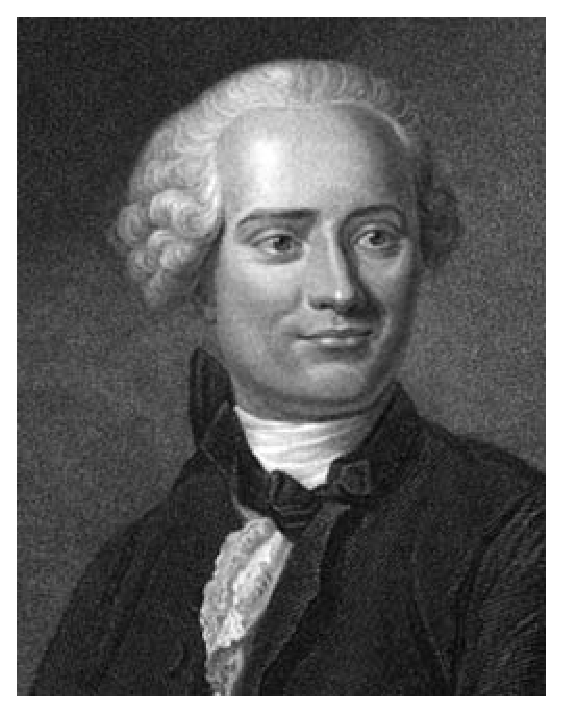
\includegraphics[width=3.5cm]{dalembert.eps}
      \captionsetup{singlelinecheck=off,justification=raggedright}%,margin={1mm,0mm}
\caption{D'Alembert}
    \end{minipage}%
       \begin{minipage}[t]{.7\textwidth}
       \vspace{0pt}
       \hspace{8mm}
   Durante el siglo XVIII, por una parte, el uso permanente de los infinitesimales dificultaba la comprensi�n de los procesos de paso al l�mite y, por otra parte, el reci�n inventado C�lculo era una herramienta maravillosa para estudiar y formular matem�ticamente multitud de fen�menos naturales. Adem�s, los resultados obtenidos eran correctos, por tanto no hab�a por qu� preocuparse mucho de la coherencia l�gica de los fundamentos, ya habr�a tiempo para ello m�s adelante.

   $\qquad$Debemos destacar, no obstante, la propuesta de Jean le Rond d'Alembert (1717 - 1783) de fundamentar el C�lculo sobre el concepto de l�mite: \emph{``La th�orie des limites est la base de la vraie M�taphysique du calcul diff�rentiel''}.
      \end{minipage}
      \end{center}
  \end{figure}\vspace*{-.5cm}

\noindent D'Alembert redact� la mayor�a de los art�culos de matem�ticas y ciencias para la obra inmortal del Siglo de las Luces la \emph{Encyclop�die, ou Dictionnaire Raisonn� des Sciences, des Arts et des M�tiers} (1751 - 65). En el art�culo Diff�rentiele (1754), despu�s de criticar la ``metaf�sica del infinito'' de Leibniz, escribe:
\begin{quote}
\footnotesize{Newton part�a de otro principio; y se puede decir que la metaf�sica de este gran ge�metra sobre el c�lculo de fluxiones es muy exacta y luminosa, aunque solamente la ha dejado entrever. �l no ha considerado nunca el c�lculo diferencial como el c�lculo de cantidades infinitamente peque�as, sino como el m�todo de las primeras y �ltimas razones, es decir, el m�todo para hallar los l�mites de las razones.

[\dots] La suposici�n que se hace de las cantidades infinitamente peque�as s�lo sirve para acortar y simplificar los razonamientos; pero en el fondo el c�lculo diferencial no precisa suponer la existencia de tales cantidades; y m�s a�n, este c�lculo consiste meramente en la determinaci�n algebraica del l�mite de una raz�n.}
\end{quote}
D'Alembert fue el primer matem�tico que afirm� haber probado que los infinitamente peque�os  \emph{``n'existent r�ellement ni dans la nature, ni dans les suppositions des G�om�tres''}. Seg�n d'Alembert:
\begin{quote}
\footnotesize{Una cantidad es algo o nada; si es algo, a�n no se ha desvanecido; si no es nada, ya se ha desvanecido literalmente. La suposici�n de que hay un estado intermedio entre estos dos es una quimera.}
\end{quote}
En el art�culo \emph{Limite} (1765), tambi�n escrito para la \emph{Encyclop�die} junto con Jean-Baptiste de La Chapelle (1710 - 1792), se da la siguiente definici�n de l�mite:
\begin{quote}
\footnotesize{Se dice que una magnitud es el l�mite de otra magnitud, cuando la segunda puede aproximarse a la primera, sin llegar nunca a excederla, en menos que cualquier cantidad dada tan peque�a como se quiera suponer.}
\end{quote}
Este art�culo tambi�n contiene los resultados sobre la unicidad del l�mite y sobre el l�mite del producto de dos magnitudes, por supuesto, enunciados ret�ricamente sin ning�n tipo de s�mbolo para representar los l�mites. Dichos resultados hab�an aparecido en el libro de La Chapelle \emph{Institutions de G�om�trie} (1757). Tanto d'Alembert como La Chapelle ten�an una idea esencialmente geom�trica del concepto de l�mite, as� el ejemplo que ponen en el citado art�culo es el de la aproximaci�n de un c�rculo por pol�gonos.

El punto de vista de d'Alembert, esencialmente correcto, no era compartido por otros matem�ticos, de forma destacada, por Joseph-Louis de Lagrange (1736 - 1813) quien en su obra \emph{Th�orie des fonctions analytiques} (1797), cuyo subt�tulo era nada menos que \emph{Les Principes du Calcul Diff�rentiel, d�gag�s de toute consid�ration d'infiniment petits, d'�vanouissants, de limites et de fluxions, et r�duits � l'analyse alg�brique des quantit�s finies}, pretendi� establecer una fundamentaci�n algebraica del C�lculo, eliminando toda referencia a los infinitesimales y a los l�mites. Lagrange criticaba la teor�a de las ``�ltimas razones'' de Newton y afirmaba:
\begin{quote}
\footnotesize{Ese m�todo tiene el gran inconveniente de considerar cantidades en el momento en que ellas cesan, por as� decir, de ser cantidades; pues aunque siempre podemos concebir adecuadamente las razones de dos cantidades en tanto en cuanto ellas permanecen finitas, esa raz�n no ofrece a la mente ninguna idea clara y precisa tan pronto como sus t�rminos ambos llegan a ser nada a la vez.} \end{quote}
Esta severa cr�tica va realmente dirigida contra Euler, quien conceb�a las cantidades infinitesimales como ceros exactos y, por tanto, un cociente de diferenciales lo interpretaba como $\frac{0}{0}$, expresi�n de la cual hab�a que hallar en cada caso ``su verdadero valor''. Lo llamativo es que la propuesta de Lagrange se basaba en los desarrollos en series de Taylor, considerados como una generalizaci�n del �lgebra de polinomios, con lo que, de hecho, estaba usando la idea de l�mite que quer�a evitar. Por otra parte, es conocida la jactancia de Lagrange de que en su monumental \emph{M�canique analytique}(1772 - 88) no hab�a usado ni necesitado ninguna figura. Lagrange segu�a as� la tendencia, cada vez mayor, de separar el c�lculo y la geometr�a. De hecho, Lagrange puede considerarse un ``matem�tico puro''; su rechazo a la teor�a de fluxiones se debe a que est� basada en la idea de movimiento, que no es matem�tica, y su rechazo de los l�mites es debido a la confusa formulaci�n de dicho concepto en su tiempo.
\subsection[El premio de la Academia de Berl�n de 1784]{El premio de la Academia de Berl�n y otras propuestas en el �ltimo tercio del siglo XVIII}
Jacques-Antoine-Joseph Cousin (1739 - 1800) escribi� un libro de texto \emph{Le�ons de Calcul Diff�rentiel et de Calcul Int�gral} (1777), en el que, siguiendo la idea de d'Alembert, afirmaba fundamentar el c�lculo sobre el concepto de l�mite, el cual, para Cousin, es el mismo que el expresado por La Chapelle en el art�culo \emph{Limite} de la \emph{Encyclop�die} antes rese�ado. En particular, no hace distinci�n entre cantidades variables y constantes.  Desde un punto de vista operativo, Cousin introduce, sin justificaci�n, un principio de conservaci�n de las razones entre dos variables por paso al l�mite. Una novedad importante es que Cousin reconoce la necesidad de un s�mbolo para expresar el l�mite, pero no hace nada al respecto.

Roger Martin (1741 - 1811) public� un libro de texto \emph{�l�ments de Math�matiques} (1781) con igual prop�sito que Cousin. La definici�n de l�mite de Martin es m�s precisa:
\begin{quote}
\footnotesize{Por el l�mite de una cantidad variable se entiende el valor o estado hacia el cual ella siempre tiende conforme var�a, sin alcanzarlo nunca; pero al cual, no obstante, puede aproximarse de manera que difiera de �l por una cantidad menor que cualquier cantidad dada.}
\end{quote}
La condici�n de peque�ez de la diferencia est� formulada en la forma que despu�s ser�a la usual, adem�s, distingue entre variable y valor constante.

En 1784 la Academia de Berlin, cuyo director era Lagrange, anunci� la convocatoria de un premio para ``una teor�a clara y precisa de lo que se llama el infinito en matem�ticas''. El prop�sito de la Academia era eliminar el uso de los infinitesimales:
\begin{quote}
\footnotesize{Es bien sabido que la geometr�a superior emplea regularmente lo \emph{infinitamente grande} y lo \emph{infinitamente peque�o}\dots La Academia, en consecuencia, desea una explicaci�n de c�mo es posible que se hayan conseguido deducir tantos teoremas correctos a partir de unos presupuestos contradictorios, as� como\dots un principio verdaderamente matem�tico que pueda sustituir correctamente al del infinito.}
\end{quote}
El premio fue concedido en 1786 a Simon-Antoine-Jean L'Huilier (1750 - 1840) por su ensayo \emph{Exposition �l�mentaire des principes des calculs sup�rieurs} en el cual L'Huilier desarrollaba una teor�a de l�mites. Su definici�n de l�mite es:
\begin{quote}
\footnotesize{Sea una cantidad variable, siempre menor o siempre mayor que una propuesta cantidad constante; pero de la cual puede diferir menos que cualquier propuesta cantidad menor que ella misma: esta cantidad constante se dice que es el l�mite por exceso o por defecto de la cantidad variable.}
\end{quote}
La novedad aqu� est� en los conceptos de ``l�mite por exceso'' y ``l�mite por defecto''. Al introducir esta distinci�n, L'Huilier observaba que hasta entonces no se hab�a tenido en cuenta el hecho de que la aproximaci�n al l�mite puede realizarse tanto desde una variable con valores crecientes como desde una variable con valores decrecientes. Por ello, L'Huilier introduce los conceptos de \emph{l�mite por la derecha} y de \emph{l�mite por la izquierda}.

En esta obra es donde, por primera, se usa el s�mbolo ``$\lim$.'' (con el punto, como si fuera una abreviaci�n de ``l�mite'') para representar el l�mite, aunque L'Huilier no lo hace de una forma regular.

El principal logro de L'Huilier fue extender la aplicabilidad del concepto de l�mite. Mientras que sus predecesores hab�an dado solamente un par de reglas b�sicas, �l realiz� un desarrollo m�s sistem�tico, probando las reglas del producto y del cociente para l�mites, y obteniendo la regla de la derivada de un producto por medio de l�mites.

En esta exposici�n estoy siguiendo muy de cerca el excelente libro de Schubring \cite{rigor}. Este autor hace un notable descubrimiento. Se trata de un ensayo de 100 p�ginas, titulado \emph{Compendio da Theorica dos Limites, ou Introduc\c{c}a\~{o} ao Methodo das Flux\~{o}es}, que fue publicado por la Academia de Ciencias de Lisboa en 1794, aunque su autor Francisco de Borja Gar\c{c}\~{a}o Stockler (1759 - 1829) lo hab�a presentado ya en 1791. Stockler naci� en Lisboa, su padre era alem�n y su madre portuguesa. Estudi� la carrera militar y tambi�n matem�ticas en la Universidad de Coimbra. Desarroll� una gran actividad tanto pol�tica como cient�fica. La importancia del citado libro de Stockler es que contiene el primer intento de una presentaci�n algebraica del concepto de l�mite. Stockler ten�a un excelente conocimiento de la literatura matem�tica de su �poca, y en su libro se apoya precisamente en los autores que hemos citado anteriormente. Pero Stockler aventaja ampliamente a sus fuentes al separar el concepto de l�mite del concepto geom�trico, algebraiz�ndolo tanto para variables como para funciones. Adem�s, es un pionero en el uso de desigualdades. Su definici�n de l�mite es la siguiente:
\begin{quote}
\footnotesize{Una cantidad constante es llamada ``L�mite'' de una variable si la �ltima puede ir aumentando o disminuyendo -- aunque sus valores nunca lleguen a ser igual al de la constante -- da tal forma que puede aproximar la constante tanto que la diferencia llega a ser menor que cualquier cantidad dada, por peque�a que esta pueda haber sido escogida.}
\end{quote}
La definici�n es parecida a la de Martin, aunque hay un mayor �nfasis en que el l�mite es un valor constante. Stockler tambi�n usa los conceptos de l�mites por la derecha y por la izquierda de L'Huilier.

Debemos notar que todas estas definiciones de l�mite que estamos dando se refieren a variables y que dichas variables suelen interpretarse como cantidades geom�tricas (�reas, longitudes de arco, medidas de �ngulos, etc.). Adem�s, una ``cantidad constante'' es interpretada generalmente como una cantidad positiva. Con frecuencia se considera que el cero tiene un car�cter especial y se dan definiciones espec�ficas para tenerlo en cuenta. Precisamente, eso es lo que hace Stockler introduciendo el concepto de \emph{``variable sin l�mite de disminuci�n''} con el significado de una variable con l�mite cero. De esta forma, tambi�n evita usar infinit�simos. Stockler establece como un resultado fundamental que
\begin{quote}
\footnotesize{Toda cantidad capaz de un l�mite, tiene necesariamente que ser igual a su l�mite, m�s o menos una cantidad variable sin l�mite de disminuci�n.}
\end{quote}
Stockler desarrolla todo un �lgebra de l�mites y no se limita a las operaciones de suma, producto y cociente. He aqu� una muestra:
\begin{quote}
\footnotesize{Una potencia $\dis a^x$, donde $a<1$ es una constante y $x$ una variable con valores positivos y sin l�mite de aumento, forma una sucesi�n nula.}
\end{quote}
Stockler explica el uso del s�mbolo ``Lim.'' para representar l�mites y lo emplea de forma operativa para permutar l�mites. Por ejemplo, si $b = \textrm{Lim.\ } x$ y $a$ es constante, $\textrm{Lim.\ }(a^x) = a^b$.

Stockler no considera solamente l�mites de variables sino tambi�n de funciones. De forma expl�cita establece la permutabilidad del l�mite con una funci�n:
\begin{quote}
\footnotesize{El l�mite de cualquier funci�n $Fx$ de una variable $x$ que es capaz de (tiene) l�mite, es igual al valor hom�logo por la funci�n de su l�mite.}
\end{quote}
Simb�licamente, Stockler expresa el teorema como sigue: Para $a=\textrm{Lim.\ } x$, se sigue que $\textrm{Lim.\ } Fx=Fa$.
\subsection{Cauchy y su \emph{Cours D'Analyse} de 1821}
A principios del siglo XIX, parec�a cada vez m�s necesario consolidar la enorme cantidad de resultados que ya se hab�an obtenido usando las t�cnicas precariamente fundamentadas del c�lculo. Hab�a llegado el momento en que se dispon�a de las herramientas necesarias para desvelar las sutilezas del concepto de l�mite, cuya lenta y trabajosa evoluci�n a lo largo del siglo XVIII acabamos de ver. Lo que se necesitaba era dar definiciones precisas, simb�licas y operativas, que no estuvieran basadas en intuiciones geom�tricas ni cinem�ticas. Para ello, hab�a que precisar las expresiones vagas que sol�an usarse, al estilo de ``aproximarse m�s que una cantidad dada, por peque�a que �sta sea'', y dotarlas de un significado matem�tico preciso que pudiera ser usado para dar demostraciones. Lo que se necesitaba era traducir las definiciones verbales de l�mite mediante el �lgebra de desigualdades que en esa �poca ya se hab�a desarrollado. Esto puede parecer f�cil visto desde nuestra perspectiva actual, pero no lo era en absoluto.

\begin{figure}[ht]
\begin{center}
     \begin{minipage}[t]{.3\textwidth}
     \vspace{3pt}
     %\hspace{2mm}
     \flushleft
      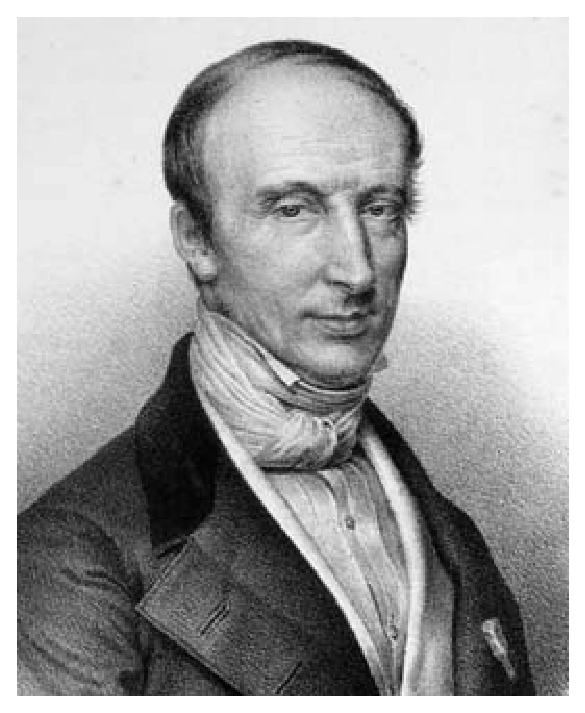
\includegraphics[width=3.5cm]{cauchy.eps}
      \captionsetup{singlelinecheck=off,justification=raggedright}%,margin={1mm,0mm}
\caption{Cauchy}
    \end{minipage}%
       \begin{minipage}[t]{.7\textwidth}
       \vspace{0pt}
       \hspace{8mm}
       Si vuelves a leer la definici�n de l�mite (\ref{def:deflimite}), puedes comprobar lo abstracta que es: no queda nada en ella de la intuici�n inicial con la que Newton imaginaba sus ``razones �ltimas''. Es una definici�n ``est�tica'' y todo en ella es aritm�tica: valor absoluto, desigualdades\dots �no contiene ninguna igualdad! Ganamos rigor a costa de la intuici�n.
   Quien realiz� la haza�a de fundamentar con rigor el c�lculo sobre el concepto de l�mite fue \href{http://www.librosmaravillosos.com/grandesmatematicos/capitulo15.html}{Augustin - Louis Cauchy} (1789 - 1857). Nos vamos a centrar aqu� exclusivamente en este aspecto de su obra, de la que nos ocuparemos con m�s detalle en un cap�tulo posterior. Conviene, no obstante decir, que hay interpretaciones muy distintas de la obra de Cauchy. En particular, se ha escrito mucho sobre el uso que Cauchy hace de los\linebreak
     \end{minipage}
      \end{center}
  \end{figure}\vspace*{-1.2cm}
\noindent infinit�simos. Creo que la documentada exposici�n que hace Schubring en \cite{rigor} es muy convincente. Su tesis es que Cauchy, por su propia voluntad, nunca hubiera dejado entrar a los infinit�simos en sus libros, pero que se vio en la necesidad de hacerlo por la presi�n del entorno de l'�cole Polytechnique donde desempe�aba su labor docente. De todas formas, su concepto de infinit�simo, como veremos enseguida, no es el de una cantidad no nula pero infinitamente peque�a. En su \emph{Cours d'Analyse de l'�cole Polytechnique} (1821), Cauchy empieza exponiendo su concepto de n�mero, de cantidad y seguidamente, en la p�gina 19, aparecen las siguientes definiciones:
\begin{quote}
\footnotesize{Se llama cantidad \emph{variable} aquella que se considera debe recibir sucesivamente varios valores diferentes unos de otros.[\dots] Cuando los valores sucesivamente atribuidos a una misma variable se aproximan indefinidamente a un valor fijo, de manera que acaban por diferir de �l tan poco como se quiera, �ste �ltimo es llamado el \emph{l�mite} de todos los otros.

[\dots] Cuando los valores num�ricos (valores absolutos) sucesivos de una misma variable decrecen indefinidamente, de manera que quedan por debajo de todo n�mero dado, esta variable recibe el nombre de \emph{infinit�simo} o de cantidad \emph{infinitamente peque�a}. Una variable de esta naturaleza tiene por l�mite a cero.}

Cuando los valores num�ricos (valores absolutos) sucesivos de una misma variable crecen m�s y m�s, de manera que permanecen por encima de todo n�mero dado, se dice que esta variable tiene por l�mite el \emph{infinito positivo}, indicado por el signo $\infty$, cuando se trata de una variable positiva, y el \emph{infinito negativo}, indicado por la notaci�n $-\infty$, cuando se trata de una variable negativa.
\end{quote}
Llama la atenci�n en esta definici�n la idea repetida de ``sucesivos valores'' que algunos autores interpretan como si Cauchy considerara a las cantidades variables como sucesiones. Aunque sigue siendo una definici�n verbal, es mucho m�s precisa que las anteriores y lo importante es la forma en que Cauchy la interpreta por medio del �lgebra de desigualdades. Podemos hacernos una idea de la forma de trabajar de Cauchy considerando el siguiente resultado que aparece en la p�gina 54 del \emph{Cours d'Analyse}. Traduzco y hago algunos comentarios que van en cursiva y entre par�ntesis.

{\small{
\noindent{\textbf{Teorema I} (Cauchy - Cours d'Analyse, p.54).} Si para valores crecientes de $x$, la diferencia
$$
f(x+1)-f(x)
$$
converge hacia un cierto l�mite $k$, la fracci�n
$$
\frac{f(x)}{x}
$$
converger� al mismo tiempo hacia el mismo l�mite.

\noindent{\emph{Demostraci�n}}. Supongamos para empezar que la cantidad $k$ tenga un valor finito, y designemos por \eps\ un n�mero tan peque�o como se quiera. Puesto que los valores crecientes de $x$ hacen converger la diferencia
$$
f(x+1)-f(x)
$$
hacia el l�mite $k$, se podr� dar al n�mero $h$ un valor suficientemente grande para que, siendo $x$ igual o mayor que $h$, la diferencia correspondiente est� constantemente comprendida entre los l�mites
$$
k-\eps,\qquad k+\eps.
$$
(\emph{Este comienzo es impecable y nosotros lo har�amos exactamente igual. Con nuestras notaciones actuales, la hip�tesis es que
$$
\dis\lim_{x\to +\infty}\big(f(x+1)-f(x)\big)=k.
$$
Por tanto, dado \epos, existe $h>0$ tal que para todo $x\ge h$ se verifica que $\abs{f(x+1)-f(x)-k}<\eps$. Eso es exactamente lo que escribe Cauchy.})

Supuesto esto, si se designa por $n$ un n�mero entero cualquiera, cada una de las cantidades
$$
\begin{array}{l}
  f(h+1)-f(h) \\
  f(h+2)-f(h+1) \\
  \dots\dots\dots\dots\dots\dots\dots\dots \\
  f(h+n)-f(h+n-1)
\end{array}
$$
y, en consecuencia, su media aritm�tica, a saber
$$
\frac{f(h+n)-f(h)}{n}
$$
se encontrar� comprendida entre los l�mites $k-\eps$, $k+\eps$. Se tendr� pues
$$
\frac{f(h+n)-f(h)}{n}=k+\alpha
$$
siendo $\alpha$ una cantidad comprendida entre los l�mites $-\eps$, $+\eps$. Sea ahora
$$
h+n=x
$$
La ecuaci�n precedente se convertir� en
\begin{equation}\label{C1}
\frac{f(x)-f(h)}{x-h}=k+\alpha,
\end{equation}
y se concluir�
\begin{eqnarray}
\nonumber   f(x) &=& f(h)+(x-h)(k+\alpha) \\
  \rule{0mm}{7mm}\dfrac{f(x)}{x} &=&  \dfrac{f(h)}{x}+\left(1-\dfrac{h}{x}\right)(k+\alpha)\label{C2}
\end{eqnarray}
(\emph{Hasta aqu�, nada que objetar. Todo es correcto.})

Adem�s, para hacer crecer indefinidamente el valor de $x$, ser� suficiente hacer crecer indefinidamente el n�mero entero $n$ sin cambiar el valor de $h$. Supongamos, en consecuencia, \marginpar{\flushright\curvasl} que en la ecuaci�n (\ref{C2}) se considera $h$ como una cantidad constante, y $x$ como una cantidad variable que converge hacia el l�mite $\infty$. Las cantidades
$$
\dfrac{f(h)}{x},\qquad \dfrac{\,h\,}{x},
$$
encerradas en el segundo miembro, converger�n hacia el l�mite cero, y el propio segundo miembro hacia un l�mite de la forma
$$
k+\alpha,
$$
$\alpha$ estando siempre comprendida entre $-\eps$ y $+\eps$. Por consiguiente, la raz�n
$$
\dfrac{f(x)}{x}
$$
tendr� por l�mite una cantidad comprendida entre $k-\eps$ y $k+\eps$. Debiendo subsistir esta conclusi�n, cualquiera que sea la peque�ez del n�mero \eps, resulta que el l�mite en cuesti�n ser� precisamente igual a la cantidad $k$. En otras palabras, se tendr�
\begin{equation}\label{C3}
    \lim\dfrac{f(x)}{x}=k=\lim[f(x+1)-f(x)].
\end{equation}
(\emph{Seguidamente, Cauchy pasa a considerar los casos en que $k=\infty$ y $k=-\infty$.})\hfill$\Box$}}

\medskip

Esta demostraci�n es notable, por su rigor y tambi�n porque \emph{no es correcta}. Te dar� un contraejemplo en un ejercicio. �Ser�as capaz de explicar a Cauchy d�nde est� el error en su razonamiento? Por supuesto, lo que interesa aqu� es la forma en que Cauchy traduce los conceptos de l�mite por medio de desigualdades. El error es anecd�tico, adem�s, cuando Cauchy emplea este resultado lo hace siempre en casos en que la tesis es correcta; por ejemplo, para la funci�n $\dis\log x$ ,se tiene que $\dis\lim_{x\to +\infty}\big(\log(x+1)-\log(x)\big)=0$ y, por tanto, $\dis\lim_{x\to +\infty}\dfrac{\log x}{x}=0$ lo cual es correcto. Si hasta el mismo Cauchy se equivocaba en cosas aparentemente f�ciles, no te extra�es si a ti te cuesta trabajo entender bien la definici�n de l�mite, esa experiencia la hemos tenido todos los que hemos estudiado An�lisis.

Durante el siglo XVIII, el concepto de continuidad no hab�a merecido nada m�s que una espor�dica atenci�n, y siempre hab�a sido considerado desde un punto de vista filos�fico, m�s como una ley de la naturaleza que como un concepto propiamente matem�tico. Generalmente la continuidad de una funci�n se entend�a en el sentido de Euler, y significaba que dicha funci�n estaba definida por una �nica expresi�n anal�tica. En su \emph{Cours d'Analyse}, Cauchy define el concepto de funci�n continua y, lo que es notable, de funci�n discontinua; y su definici�n es realmente muy minuciosa. Dice as�:
\begin{quote}
\footnotesize{Sea $f(x)$ una funci�n de la variable $x$, y supongamos que, para cada valor de $x$ comprendido entre ciertos l�mites dados, esta funci�n admite constantemente un valor �nico y finito. Si, partiendo de un valor de $x$ comprendido entre estos l�mites, se atribuye a la variable $x$ un incremento infinitamente peque�o $\alpha$, la funci�n misma recibir� por incremento la diferencia
$$
f(x+\alpha)-f(x)
$$
que depender� a la vez de la nueva variable $\alpha$ y del valor de $x$. Dicho esto, la funci�n $f(x)$ ser�, entre los dos l�mites asignados a la variable $x$, funci�n \emph{continua} de esta variable, si, para cada valor de $x$ intermedio entre estos l�mites, el valor num�rico (valor absoluto) de la diferencia
$$
f(x+\alpha)-f(x)
$$
decrece indefinidamente con el de $\alpha$. En otras palabras, \emph{la funci�n $f(x)$ permanecer� continua con respecto a $x$ entre los l�mites dados, si, entre estos l�mites un incremento infinitamente peque�o de la variable produce siempre un incremento infinitamente peque�o de la funci�n}.

Se dice tambi�n que la funci�n $f(x)$ es, en un entorno de un valor particular atribuido a la variable $x$, funci�n continua de esta variable, siempre que ella sea continua entre dos l�mites de $x$, por cercanos que est�n, que encierren al valor considerado. Finalmente, cuando una funci�n deja de ser continua en el entorno de un valor particular de la variable $x$, se dice entonces que ella se hace \emph{discontinua} y que para este valor particular de $x$ hay una \emph{soluci�n de continuidad}}.
\end{quote}
Cauchy da realmente dos definiciones; primero define lo que nosotros llamar�amos ``continuidad en un intervalo'' y, despu�s, la continuidad puntual. La primera definici�n ha sido interpretada en el sentido de que lo que Cauchy entiende por continuidad es lo que ahora llamamos ``continuidad uniforme''.

Seguidamente a esta definici�n, Cauchy pasa a estudiar la continuidad de las funciones elementales, considerando en cada caso, los l�mites entre los que cada funci�n es continua. Despu�s demuestra el teorema de los valores intermedios (teorema de Bolzano) del cual da dos demostraciones. Una que se apoya de forma decisiva en la intuici�n geom�trica y, en una nota al final del texto, otra, que �l califica de ``puramente anal�tica'', que consiste en el m�todo de bisecci�n, en la que Cauchy usa, sin demostraci�n ni comentario, que una sucesi�n mon�tona acotada es convergente, propiedad que equivale a la completitud del sistema de los n�meros reales.

El citado texto de Cauchy, as� como los libros \emph{R�sum� des le\c{c}ons sur le Calcul Infinit�simal} (1823) y \emph{Le\c{c}ons sur le Calcul Diff�rentiel} (1829), en los que se recogen los cursos impartidos por Cauchy en la �cole Polytechnique durante los a�os precedentes, tuvieron una gran influencia y establecieron nuevas exigencias de rigor. En el c�lculo de Cauchy los conceptos de funci�n y de l�mite son los conceptos fundamentales.
\subsection{El innovador trabajo de Bolzano}
\begin{figure}[ht]
\begin{center}
     \begin{minipage}[t]{.3\textwidth}
     \vspace{0pt}
     %\hspace{2mm}
     \flushleft
      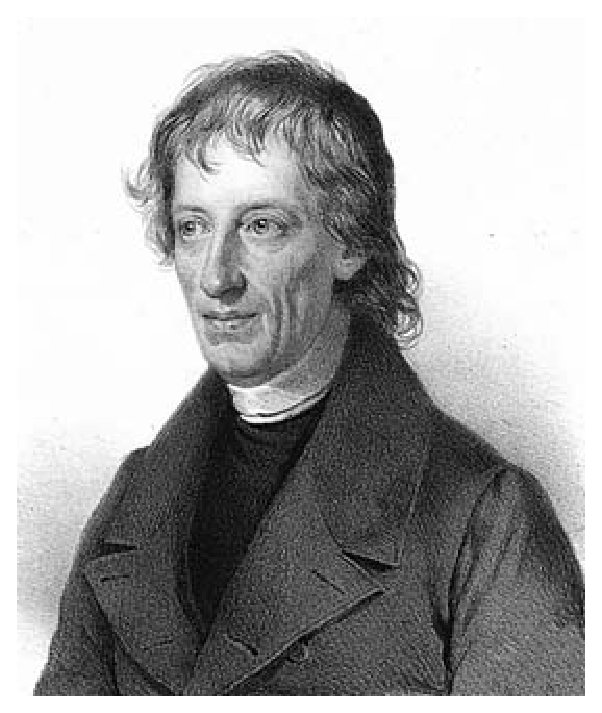
\includegraphics[width=3.5cm]{bolzano.eps}
      \captionsetup{singlelinecheck=off,justification=raggedright}%,margin={1mm,0mm}
\caption{Bolzano}
    \end{minipage}%
       \begin{minipage}[t]{.7\textwidth}
       \vspace{0pt}
       \hspace{8mm}
   Es obligado citar a \href{http://es.wikipedia.org/wiki/Bernard_Bolzano}{Bernhard Bolzano} (1781 - 1848), matem�tico, l�gico y fil�sofo, profesor en la Universidad de su ciudad natal, Praga, desde 1805 a 1820. Bolzano, cuyas obras completas comprender�n, cuando terminen de editarse, alrededor de 140 vol�menes, fue un innovador en todos los campos que trabaj�. En sus trabajos matem�ticos anticip� muchos de los conceptos que posteriormente redescubrieron y desarrollaron matem�ticos como Cauchy, Weierstrass o Cantor. Debido a su relativo aislamiento en la ciudad de Praga, en una �poca en la que el centro de toda la producci�n matem�tica estaba en Par�s, la obra matem�tica de Bolzano fue poco conocida y no tuvo la influencia que merec�a por su rigor y profundidad.
     \end{minipage}
      \end{center}
  \end{figure}\vspace*{-.7cm}
Por lo que a la continuidad de una funci�n se refiere, Bolzano public� en 1817 un peque�o libro de 60 p�ginas \emph{Purely analytic proof of the theorem that between any two values which give results of opposite sign there lies at least one real root of the equation} \cite{bolzano}, en el que, entre otras cosas, demuestra el teorema que ahora lleva su nombre. Bolzano empieza razonando que las demostraciones conocidas de ese teorema eran inapropiadas. La claridad de ideas con que se expresa es muy llamativa (traduzco de \cite{bolzano}):
\begin{quote}
\footnotesize{
No obstante, un examen m�s cuidadoso muestra muy pronto que ninguna de estas pruebas puede considerarse adecuada.

I.$\quad$ El tipo de demostraci�n m�s usual depende de una verdad pedida en pr�stamo a la geometr�a, a saber, que toda l�nea continua de curvatura simple cuyas ordenadas son primero positivas y despu�s negativas (o rec�procamente) necesariamente debe intersecar en alg�n lugar al eje de abscisas en un punto comprendido entre aquellas ordenadas. Ciertamente, nada  hay que objetar respecto a la correcci�n, ni tampoco a la obviedad, de esta proposici�n geom�trica. Pero est� claro que es una intolerable ofensa contra el m�todo correcto, deducir verdades de las matem�ticas puras (o generales, i.e. aritm�tica, �lgebra, an�lisis) a partir de consideraciones que pertenecen simplemente a una parte aplicada (o especial), a saber, la geometr�a.

[\dots] Consideremos ahora la raz�n objetiva por la que una l�nea en las circunstancias antes mencionadas interseca el eje de abscisas. Sin duda, todo el mundo ver� enseguida que esta raz�n descansa en nada m�s que en el asentimiento general, como consecuencia del cual toda funci�n continua de $x$ que sea positiva para alg�n valor de $x$, y negativa para otro, debe ser cero para alg�n valor intermedio de $x$. Y �sta es, precisamente, la verdad que debe ser probada.

II.$\quad$ No menos reprobable es la demostraci�n que algunos han construido a partir del concepto de la continuidad de una funci�n con la inclusi�n de los conceptos de tiempo y movimiento. [\dots] Esto es adicionalmente ilustrado por el ejemplo del movimiento de dos cuerpos, uno de los cuales est� inicialmente detr�s del otro y posteriormente delante del otro. Necesariamente se deduce que en un tiempo debe haber estado al lado del otro. Nadie negar� que los conceptos de tiempo y movimiento son tan extra�os a la matem�tica general como el concepto de espacio. No obstante, si estos conceptos fueran introducidos solamente por motivos de claridad, no tendr�amos nada en contra de ello. [\dots] Por tanto, debe observarse que no consideramos que los ejemplos y aplicaciones disminuyan en lo m�s m�nimo la perfecci�n de una exposici�n cient�fica. De otra manera, estrictamente exigimos s�lo esto: que los ejemplos nunca sean empleados como argumentos en lugar de las demostraciones, y que la esencia de una deducci�n nunca est� basada sobre el uso meramente metaf�rico de frases o sobre sus ideas relacionadas, de forma que la deducci�n misma quedar�a vac�a tan pronto como �stas fueran cambiadas.}
\end{quote}
Es dif�cil expresarse con m�s claridad que como lo hace Bolzano. Su definici�n de continuidad, en el citado trabajo, es como sigue:
\begin{quote}
\footnotesize{Una funci�n $f(x)$ var�a seg�n la ley de continuidad para todos los valores de $x$  dentro o fuera de ciertos l�mites, significa exactamente que: si $x$ es alg�n tal valor, la diferencia $f(x+\omega)-f(x)$ puede ser hecha m�s peque�a que cualquier cantidad dada, supuesto que $\omega$ puede ser tomado tan peque�o como queramos.}
\end{quote}
Seguidamente, Bolzano establece un teorema previo cuyo asombroso enunciado es como sigue:
\begin{quote}
\footnotesize{Si una propiedad $M$ no pertenece a todos los valores de una variable $x$, pero s� pertenecen todos los valores que son menores que un cierto $u$, entonces existe siempre una cantidad $U$ que es la mayor de aquellas de las cuales puede afirmarse que toda m�s peque�a $x$ tiene la propiedad $M$.}
\end{quote}
Comprendes por qu� califico de ``asombroso'' ese enunciado, �verdad? �Es la propiedad de extremo inferior!�En el a�o 1817, 55 a�os antes de que Dedekind y Cantor publicaran sus teor�as de los n�meros reales!

El conocido historiador de las matem�ticas Ivor Grattan - Guinness, en un pol�mico trabajo titulado \emph{Bolzano, Cauchy and the ``New Analysis'' of Early Nineteenth Century} \cite{grattan}, expresa su opini�n de que Cauchy conoc�a el trabajo de Bolzano pero nunca lo reconoci�. Desde luego, ni en las numerosas obras de Cauchy, ni en su correspondencia particular, se ha encontrado ninguna referencia a Bolzano, por lo que la afirmaci�n de Grattan - Guinness, como �l mismo reconoce, no est� sustentada en pruebas documentales.
\subsection{Weierstrass nos dio los $\varepsilon-\delta$}
\begin{figure}[ht]
\begin{center}
     \begin{minipage}[t]{.3\textwidth}
     \vspace{0pt}
     %\hspace{2mm}
     \flushleft
      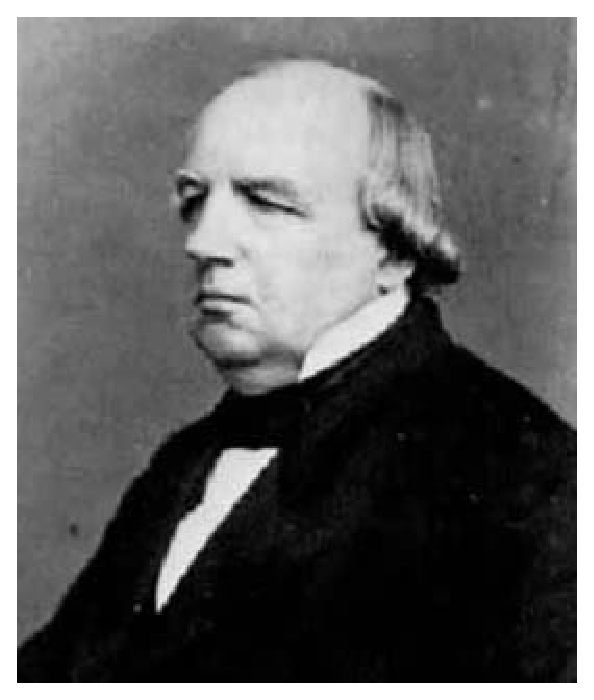
\includegraphics[width=3.5cm]{weierstrass.eps}
      \captionsetup{singlelinecheck=off,justification=raggedright}%,margin={1mm,0mm}
\caption{Weierstrass}
    \end{minipage}%
       \begin{minipage}[t]{.7\textwidth}
       \vspace{-3pt}
       \hspace{8mm}
       Una caracter�stica de los textos citados de Cauchy es que en ellos no hay ni una sola figura. Cauchy liber� al c�lculo de sus ataduras geom�tricas, aunque todav�a sus definiciones conten�an t�rminos imprecisos como ``tan peque�o como queramos'' y ``disminuir  indefinidamente hasta converger al l�mite cero'', o ideas de movimiento como ``variable que se acerca a un l�mite'' por no hablar de sus ``infinitamente peque�os''. Para seguir avanzando era necesario acabar de una vez con las distinciones entre n�mero y cantidad. Los n�meros reales todav�a eran considerados geom�tricamente y no se hab�an establecido sus propiedades de forma expl�cita. El cero y los n�meros negativos eran vistos a�n por muchos matem�ticos como algo de naturaleza diferente a los n�meros positivos.
               \end{minipage}
      \end{center}
  \end{figure}\vspace*{-.8cm}
En definitiva, deb�a concretarse el significado de expresiones como ``cantidad variable'' y ``variable continua''. Tambi�n era preciso separar la idea de funci�n de su representaci�n anal�tica concreta, lo cual, como ya vimos en el Cap�tulo 2, fue hecho por Dirichlet en 1837 con su definici�n general de funci�n como correspondencia arbitraria. Finalmente, pero no menos importante, estaban las cuestiones referentes a la convergencia de sucesiones y series num�ricas y funcionales, a�n mal comprendidas en la �poca de Cauchy, de las que nos ocuparemos en otro lugar.

En los cincuenta a�os que van de 1830 a 1880 se lograron desentra�ar todas estas cuestiones fundamentales gracias, principalmente, a los trabajos de Dirichlet, Riemann, Weierstrass,\linebreak Dedekind y Cantor. Ya conocemos una parte de este complejo proceso, la que culmina en 1872 con la fundamentaci�n del sistema de los n�meros reales por Dedekind y Cantor.

Fue \href{http://www-groups.dcs.st-and.ac.uk/~history/Biographies/Weierstrass.html}{Karl Weierstrass} (1815 - 1897) quien llev� a sus �ltimas consecuencias el proceso de ``aritmetizaci�n del An�lisis''. Weierstrass era un desconocido profesor de instituto, cuando en 1854 public� un trabajo sobre las funciones abelianas que caus� sensaci�n en la comunidad matem�tica. Poco despu�s, en 1856, Weierstrass ya era profesor de la Universidad de Berl�n. Los cursos que Weierstrass imparti� en Berl�n durante m�s de treinta a�os atrajeron a numerosos matem�ticos de toda europa. Disc�pulos suyos fueron, entre muchos otros menos conocidos, George Cantor (1845 - 1918), Sonya Kovalevsky (1850 - 1891), Max Planck (1858 - 1947) y David Hilbert (1862 - 1943).

Weierstrass estaba convencido de que el An�lisis deb�a ser liberado de los razonamientos geom�tricos y de los conceptos intuitivos de espacio, tiempo y movimiento y deb�a ser  fundamentado sobre los enteros positivos. Acometi� la tarea de revisar radicalmente los conceptos fundamentales del An�lisis y a este fin dedic� algunos de sus cursos. Entre otras cosas, desarroll� en ellos una teor�a aritm�tica de los n�meros reales parecida a la de Cantor. Aunque Weierstrass no public� mucho, su influencia fue enorme y sus conferencias magistrales fueron difundidas por toda Europa por sus numerosos alumnos. Weierstrass es considerado como el m�s grande analista del �ltimo tercio del siglo XIX y se le ha llamado ``el padre del an�lisis moderno''. M�s adelante tendremos ocasi�n de exponer algunas de sus contribuciones.

Por lo que al concepto de l�mite funcional se refiere, Weierstrass tradujo por medio de desigualdades y de valores absolutos las definiciones verbales de l�mite y de continuidad dadas por Cauchy y Bolzano. Para Weierstrass, una variable solamente es un s�mbolo que sirve para designar cualquier elemento del conjunto de valores que se le pueden atribuir. Una variable continua es aquella cuyo conjunto de valores no tiene puntos aislados. La definici�n de l�mite dada por Weierstrass, tal como la recogi� en sus notas el matem�tico H.E. Heine (1821 - 1881) es la siguiente:
\begin{quote}
\footnotesize{Se dice que $L$ es el l�mite de una funci�n $f(x)$ para $x=x_0$ si, dado cualquier \eps, existe un $\delta_0$ tal que para $0<\delta<\delta_0$, la diferencia $f(x_0\pm\delta)-L$ es menor en valor absoluto que \eps.}
\end{quote}
Cuando una teor�a ha sido desarrollada, llega el momento del rigor. As� el concepto de l�mite, fundamental en c�lculo porque en �l se basan los de continuidad, derivada, integral y los distintos tipos de convergencia, y es el concepto que confiere al c�lculo su caracter�stica distintiva, solamente pudo ser expresado de forma rigurosa (seg�n nuestros criterios actuales) en el �ltimo tercio del siglo XIX, despu�s de haberse estado usando, de forma m�s o menos disfrazada por los infinit�simos y otros conceptos afines como el movimiento, durante doscientos a�os. Curiosamente, la letra griega \eps, que usaba Cauchy con un significado de ``error'', se ha convertido en el paradigma de la precisi�n en nuestras actuales definiciones heredadas de Weierstrass.

La flechita en la notaci�n para l�mites, $\dis\lim_{x\to x_0}f(x)$, fue introducida por G.H. Hardy (1877 - 1947) en su notable libro \emph{A Course of Pure Mathematics} (1908).

\begin{ejercicios propuestos}
\propuesto Considera la funci�n \func{f}{\Rp}\ dada por
$$
f(x)=\dfrac{1}{1-x+E(x)}
$$
Donde, como de costumbre, $E(x)$ es la parte entera de $x$. Estudia los l�mites en $+\infty$ de las funciones $f(x+1)-f(x)$ y $\dfrac{f(x)}{x}$.
\end{ejercicios propuestos}

\section{Breve historia del infinito}
Es conocida la exclamaci�n de  David Hilbert \emph{�El infinito! Ninguna cuesti�n ha conmovido tan profundamente el esp�ritu del hombre}. Es verdad, el infinito atrae poderosamente nuestra imaginaci�n. �Qui�n no ha gritado en su infancia para devolver un agravio ``\emph{\dots y t� diez veces m�s\dots �infinitas veces m�s que yo!}''? Es dif�cil imaginar que el tiempo tuviera un comienzo y tambi�n que el espacio sea finito, porque no podemos pensar en una frontera para el espacio tras de la cual no exista m�s espacio, ni un origen para el tiempo antes del cual no hubiera tiempo. Cualquier respuesta a estas preguntas conduce siempre a nuevas preguntas. Un error t�pico consiste en creer que si algo fuera infinito deber�a contener todas las cosas, algo as� como el Aleph borgiano. Matem�ticamente, es claro que no tiene por qu� ser as�: los n�meros pares son infinitos y no son todos los n�meros. Algo infinito tampoco tiene por qu� ser necesariamente muy grande. El Aleph de la narraci�n de Borges es una peque�a esfera, un conjunto fractal contiene infinitas copias de s� mismo, el veloz Aquiles permanece corriendo sin alcanzar jam�s a la tortuga que le lleva unos pocos metros de ventaja\dots .
\subsection{La idea de infinito en la filosof�a y la matem�tica Griegas}
\subsubsection{Las apor�as de Zen�n de Elea}
\vspace*{-.5cm}
\begin{minipage}[t]{.57\textwidth}
\vspace{0pt}
\phantom{aaaaaaaaaaaaaaaaaaaaaaaaaaaaaaaaaaaaaaaaaaaaa}
\end{minipage}%
\begin{minipage}[t]{.43\textwidth}
\vspace{0pt}
{\small \textit{�Zen�n, cruel Zen�n, Zen�n de Elea!\\ Me has traspasado con la flecha alada. \\ Que, cuando vibra volando, no vuela.\\ Me crea el son y la flecha me mata. \\ �Oh sol, oh sol! �Qu� sombra de tortuga \\ Para el alma: si en marcha Aquiles, quieto!} \\  Paul Valery}
\end{minipage}

\smallskip

Un griego llamado Zen�n, del que se sabe muy poco y de forma indirecta a trav�s del \emph{Parm�nides} de Plat�n, cuyo nacimiento se fecha hacia el a�o 490 a.C en la ciudad de Elea en el sur de Italia, y que fue disc�pulo de Parm�nides, sigue manteniendo desde hace 2300 a�os su permanente desaf�o a la raz�n.

Te recuerdo que, seg�n Parm�nides, el ser es necesariamente uno, eterno, continuo, indivisible e inmutable. Los cambios, transformaciones y multiplicaci�n de los seres, son meras apariencias a las cuales no responde realidad alguna. La filosof�a de Parm�nides fue muy criticada porque choca con nuestras creencias m�s b�sicas sobre la realidad.

Zen�n ide� sus paradojas o apor�as (proposiciones sin salida l�gica) para desacreditar a quienes negaban las ideas de Parm�nides, y afirmaban la realidad del cambio y la pluralidad de los seres. Arist�teles califica a Zen�n de ``inventor de la dial�ctica'', una elaborada forma de razonamiento que consiste en probar al oponente que de sus ideas se deducen consecuencias inaceptables. Los argumentos de Zen�n son realmente del tipo ``reducci�n al absurdo'': se acepta provisionalmente una hip�tesis y, razonando correctamente a partir de ella, se llega a una conclusi�n inaceptable, lo que obliga a rechazar la hip�tesis inicial.

Vamos a exponer, en lenguaje actual, tres de las paradojas de Zen�n que van dirigidas contra las dos teor�as del movimiento sostenidas en la antig�edad, las cuales dependen, claro est�, de la supuesta naturaleza del tiempo y del espacio. Debes tener en cuenta que Zen�n no niega el movimiento sino su inteligibilidad; la afirmaci�n de que ``el movimiento se demuestra andando'' no refuta a Zen�n, su desaf�o no es a la experiencia sensible sino a la raz�n.

Las dos primeras paradojas parten del supuesto de que el espacio y el tiempo son \emph{infinitamente divisibles} y el movimiento continuo y uniforme.

\noindent\textbf{La dicotom�a.}\vspace*{-4mm}
\begin{quote}
\small{Para que un m�vil pueda llegar a un punto dado, debe recorrer primero la mitad de la distancia; pero antes de alcanzar esa mitad debe recorrer la mitad de la mitad. Y as� sucesivamente, ``ad infinitum''. De este modo para alcanzar completamente cualquier distancia tendr�a que recorrer un n�mero infinito de divisiones, lo cual es imposible en un tiempo finito.}
\end{quote}
\noindent\textbf{Aquiles y la tortuga.}\vspace*{-4mm}
\begin{quote}
\small{Aquiles, el de los pies ligeros, nunca alcanzar� a la tortuga que avanza lentamente unos cuantos metros por delante de �l. Pues cuando Aquiles alcance el punto donde estaba la tortuga, �sta ya estar� un poco m�s adelante; y cuando de nuevo Aquiles alcance ese lugar, la tortuga habr� avanzado un poco m�s. Sin desanimarse, sigue corriendo, pero al llegar de nuevo donde estaba la tortuga, esta ha avanzado un poco m�s\dots . De este modo, la tortuga estar� siempre por delante de Aquiles.}
\end{quote}
Ambos argumentos est�n relacionados. Seg�n la Dicotom�a, para que haya movimiento debe haber un comienzo, pero no hay una distancia m�nima con la que empezar; por tanto el movimiento no puede empezar, luego no hay movimiento. Seg�n Aquiles, un m�vil para alcanzar su destino debe cubrir primero la mitad de la distancia que lo separa, pero antes deber� recorrer la mitad de esa mitad, y as� sucesivamente; luego debe recorrer infinitas divisiones lo cual es imposible en tiempo finito, por tanto nunca alcanzar� su destino. Es decir, una vez empezado, el movimiento no puede parar.

La tercera paradoja, que se refiere a una flecha lanzada al aire, supone que el espacio y el tiempo est�n formados por \emph{unidades m�nimas indivisibles} y el movimiento es una sucesi�n de diminutos saltos consecutivos.

\noindent\textbf{La flecha.}\vspace*{-4mm}
\begin{quote}
\small{En un instante indivisible de tiempo la flecha debe permanecer quieta, pues si se moviera el instante contendr�a unidades de tiempo m�s peque�as en las que dicho movimiento tendr�a lugar en contra de lo supuesto. Por tanto, en cada instante la flecha est� quieta y, como el tiempo se compone de instantes, la flecha est� siempre quieta y el movimiento no tiene lugar.}
\end{quote}
La influencia de las apor�as de Zen�n en filosof�a, l�gica y matem�ticas ha sido notable y se ha escrito y se sigue escribiendo mucho sobre ellas (\cite{zenon} es una de las referencias m�s interesantes). M�s adelante veremos algunos intentos, bastante ingenuos, de resolver las dos primeras por medio de la teor�a de series. Despidamos a Zen�n con una cita de Borges.
\begin{quote}
\small{\emph{Zen�n es incontestable, salvo que confesemos la idealidad del espacio y del tiempo. Aceptemos el idealismo, aceptemos el crecimiento concreto de lo percibido, y eludiremos la pululaci�n de abismos de la paradoja. �Tocar a nuestro concepto del universo, por ese pedacito de tiniebla griega?, interrogar� mi lector.}}

\hfill{J.L. Borges, ``La perpetua carrera de Aquiles y la tortuga''.}
\end{quote}
\subsubsection{Atomismo y divisibilidad infinita}
El fil�sofo Anaximandro (\emph{ca.}610 - 546 a.C.) introdujo el infinito en la filosof�a Griega. Afirm� que el principio de todas las cosas existentes es el \emph{�peiron}. Etimol�gicamente \emph{�peiron} significa \emph{lo sin l�mites}. Seg�n Anaximandro, el \emph{�peiron} es infinito, porque provee la energ�a para que en el mundo no cese la generaci�n y corrupci�n, e indeterminado, porque no es concreto y no se identifica con ninguno de los elementos agua, aire, tierra, fuego. Podemos interpretarlo como la fuente de energ�a primordial que garantiza la transformaci�n y la unidad del cosmos.

En el per�odo que separa a Zen�n de Elea de Arist�teles surgi� la filosof�a del atomismo, iniciada por Leucipo (\emph{ca.} 450 - 420 a.C.) y desarrollada por Dem�crito (\emph{ca.} 460 - 370 a.C.). El atomismo es una filosof�a materialista que se ha interpretado como una respuesta al idealismo de la Escuela Ele�tica (Parm�nides, Zen�n). Los atomistas mantienen que hay dos principios fundamentales: los �tomos y el vac�o. Los �tomos son indivisibles e invisibles, infinitos en n�mero y de diversas formas y tama�os, perfectamente s�lidos, indestructibles y permanentes. Las substancias materiales son producidas por la uni�n y separaci�n de esos �tomos movi�ndose en el vac�o. El movimiento se produce por la reordenaci�n de los �tomos entre s�; seg�n Arist�teles, los atomistas reducen todo cambio a un mero cambio de lugar. Los atomistas admiten la pluralidad y el movimiento y niegan la infinita divisibilidad del espacio y la materia.

El atomismo fue cuestionado por \href{http://es.wikipedia.org/wiki/Arist\%C3\%B3teles}{Arist�teles} (384 - 322 a.C.), que realiz� un an�lisis sistem�tico del continuo. Arist�teles divide las cantidades en discretas y continuas. Los n�meros y el lenguaje hablado son discretas y las l�neas, superficies, s�lidos, tiempo y espacio son continuas.
La respuesta a la pregunta de si una magnitud continua (un \emph{continuo}) es permanentemente divisible en partes cada vez m�s peque�as, o hay un l�mite m�s all� del cual no puede proseguirse el proceso de divisi�n, depende de la naturaleza del infinito. Arist�teles dedica el Libro III de su \emph{F�sica} a un estudio sistem�tico del infinito. Considera que el estudio del infinito forma parte del estudio de la naturaleza, pues lo caracter�stico de �sta es el movimiento y el cambio, y el movimiento es pensado como algo continuo, y lo que es continuo es definido con frecuencia como algo infinitamente divisible.

Primero, dice Arist�teles, \emph{``hay que examinar en general si es o no es posible que haya un cuerpo sensible infinito''}. Despu�s del correspondiente estudio, llega a la conclusi�n de que \emph{``no existe un cuerpo que sea actualmente infinito''}. Pero \emph{``la negaci�n absoluta del infinito es una hip�tesis que conduce a consecuencias imposibles''}.

Arist�teles expone algunas razones que apoyan la creencia en la realidad del infinito y considera los distintos sentidos de dicho t�rmino. Entre las primeras: la infinitud del tiempo, la divisibilidad de las magnitudes y la infinitud de los n�meros; entre los segundos: lo que no puede ser recorrido o se puede recorrer pero sin llegar a un t�rmino.
\begin{quote}
\footnotesize{Es tambi�n evidente que no es posible que lo infinito exista como un ser en acto o como una substancia y un principio. Luego lo infinito existe como un atributo.}
\end{quote}
Lo infinito es un atributo que puede predicarse de la cantidad o de determinados procesos; especialmente, los procesos de adici�n y de divisi�n. Arist�teles, habla en ese sentido del infinito por adici�n y el infinito por divisi�n o la divisibilidad infinita de un continuo.
\begin{quote}
\footnotesize{Ahora bien, el ser se dice o de lo que es en potencia o de lo que es en acto, mientras que el infinito es o por adici�n o por divisi�n. Y ya se ha dicho que la magnitud no es actualmente infinita [\dots] Nos queda, entonces, por mostrar que el infinito existe potencialmente.

Pero la expresi�n ``existencia potencial'' no se debe tomar en el sentido en que se dice, por ejemplo, ``esto es potencialmente una estatua, y despu�s ser� una estatua'', pues no hay un infinito tal que despu�s sea en acto. Y puesto que el ser se dice en muchos sentidos, decimos que el infinito ``es'' en el sentido en que decimos ``el d�a es''.}
\end{quote}
Arist�teles distingue, pues, dos clases de infinito: el infinito como una totalidad completa, que llama el infinito actual y cuya existencia niega; y el infinito potencial, que concibe como un proceso secuencial de adici�n o de subdivisi�n sin final. Lo met�fora del d�a es muy apropiada, pues el \emph{ser} de un d�a es un \emph{estar siendo} de forma sucesiva, de manera que en ning�n momento el d�a queda realizado plenamente como un todo. An�logamente, el infinito potencial nunca ser� plenamente realizado \emph{pues no hay un infinito tal que despu�s sea en acto}. La infinitud potencial es la forma usual en que concebimos el tiempo como una l�nea recta indefinidamente prolongable o la sucesi�n de los n�meros que podemos ir formando por adici�n consecutiva de la unidad.

Esta concepci�n aristot�lica del infinito se acept� sin mayores cambios hasta el siglo XIX. Es una teor�a que plantea bastantes dificultades, algunas de ellas consecuencia de las ideas sobre el espacio y el tiempo del propio Arist�teles, y otras internas a la propia teor�a. La forma en que la existencia potencial del infinito se relaciona con su existencia como un proceso no es f�cil de interpretar, pues si el infinito actual nunca es posible, es preciso que haya un sentido en el cual un proceso que est� ocurriendo en el presente mantenga su existencia potencial. Por otra parte, Arist�teles mantiene que el tiempo es infinito lo que, aparentemente, contradice la no existencia de infinitos actuales. Respecto al espacio, afirma que es finito y \emph{``resulta entonces razonable pensar que no hay un infinito por adici�n que sea tal que pueda superar toda magnitud''}. Esto puede interpretarse como que Arist�teles niega la posibilidad, incluso potencial, de un infinito por adici�n de magnitudes. De todas formas, Arist�teles cree que la negaci�n del infinito actual no afecta a los matem�ticos:
\begin{quote}
\footnotesize{Esta argumentaci�n no priva a los matem�ticos de sus especulaciones por el hecho de excluir que el infinito por adici�n pueda recorrerse en acto. Porque no tienen necesidad de este infinito ya que no hacen uso de �l, sino s�lo, por ejemplo, de una l�nea finita que se prolongue tanto como ellos quieran.}
\end{quote}
Sobre todo esto se ha escrito y se sigue escribiendo mucho. M�s interesante para nosotros es la relaci�n del infinito con la divisibilidad infinita del continuo.

Los atomistas negaban la divisibilidad infinita. Su argumento era que si una magnitud continua fuera dividida en todo punto, entonces no quedar�a nada o solamente quedar�an puntos sin extensi�n, porque en caso contrario el proceso de divisi�n podr�a proseguir. Pero, dec�an, si quedan puntos sin extensi�n, entonces no es posible recomponer la magnitud original a partir de ellos, pues por la agregaci�n de puntos sin extensi�n no puede lograrse nunca una magnitud finita. Conclu�an que en cualquier caso la magnitud inicial se ha convertido en algo incorp�reo y, por tanto, algo que ten�a existencia ha dejado de ser, lo cual, evidentemente, es un imposible.

Arist�teles defend�a la divisibilidad infinita pero deb�a refutar el argumento atomista. Su soluci�n es muy original, pues afirma que aunque una magnitud continua puede ser dividida en cualquier punto, no puede ser dividida en todo punto. Para Arist�teles, dividir un continuo en todos sus puntos es reducirlo a lo discreto. Mientras que un continuo tiene la propiedad de densidad, es decir, entre dos cualesquiera de sus puntos siempre hay otro punto del continuo, los puntos obtenidos, despu�s de una divisi�n infinita actual de un continuo, ser�an adyacentes unos con otros, y  esto implica que la propiedad de densidad se habr�a perdido. Pero si dividimos un continuo, lo que obtenemos son dos continuos cada uno de ellos con la propiedad de densidad. Por tanto, es imposible llegar, por divisiones sucesivas, a reducir un continuo a puntos. As�, Arist�teles afirma la divisibilidad infinita pero niega la divisibilidad en todo punto, con lo que el argumento atomista deja de tener valor.

Esta es una posible interpretaci�n de los argumentos de Arist�teles sobre la divisibilidad infinita, que a veces son bastante oscuros y confusos. Adem�s, como veremos m�s adelante, puede darse una interpretaci�n matem�tica rigurosa de la misma.

Las matem�ticas griegas evitan el infinito actual. As�, Euclides, considera rectas que pueden ser prolongadas cuanto se quiera, pero no ``rectas infinitas''. Igualmente, al enunciar que los n�meros primos son infinitos, lo expresa diciendo que \emph{``Hay m�s n�meros primos que cualquier cantidad de n�meros primos propuesta''}. De esta forma evita considerar el infinito actual de los n�meros primos.

En \emph{Los Elementos} Euclides expone el \emph{m�todo de exhausci�n} (\ref{pag:exhauscion}) de Eudoxo de Cnido, que se utilizaba para calcular �reas (cuadraturas) de regiones planas. Es frecuente afirmar que este m�todo consiste en una aproximaci�n al �rea seguida de un proceso l�mite. No es as�. Aunque su nombre sugiere ``agotamiento'' de una figura plana por pol�gonos inscritos, el m�todo estaba basado en un razonamiento muy cuidadoso de doble reducci�n al absurdo (llamado razonamiento \emph{apag�gico}), precisamente para evitar la consideraci�n de un infinito actual.

Menci�n aparte merece Arqu�medes. Por una parte, prob� en su obra \emph{El arenario} que si el Universo estuviera completamente lleno de granos de arena, su n�mero ser�a finito. Para lo cual desarrolla un sistema de numeraci�n apropiado para manejar grandes n�meros (para los griegos el n�mero mayor era la mir�ada de mir�adas, equivalente a $10^8$) que le permite describir un n�mero que, en base diez, tendr�a unos 80000 millones de millones de cifras. Pero tambi�n Arqu�medes ide� m�todos heur�sticos\footnote{Por \emph{m�todo heur�stico} se entiende cualquier proceso que facilite anticipar un resultado. Son m�todos que se apoyan en alguna forma de intuici�n que conduce a la formulaci�n de conjeturas razonables, que despu�s deben ser probadas con m�todos cient�ficos rigurosos} que est�n expuestos en su obra \emph{El M�todo} (ver \ref{pag:metodo}), descubierta en 1906, en la que explica c�mo anticip� algunos de sus descubrimientos por medio de t�cnicas de equilibrio usando la ley de la palanca. En estas t�cnicas, Arqu�medes hace un uso muy libre del infinito; por ejemplo, descompone �reas planas como sumas infinitas de segmentos, es decir, reduce un continuo a elementos indivisibles, con lo cual podr�an estar de acuerdo los atomistas, pero no Arist�teles.

\subsubsection{La rueda de Arist�teles}
As� se conoce un interesante problema propuesto por Arist�teles en su
\emph{Mechanica}. Si un c�rculo de radio $r$ gira sin deslizar sobre su tangente horizontal, al completar un ciclo habr� avanzado una distancia igual a $2\pi r$. Consideremos dos c�rculos $C_1$ y $C_2$, de radios $r_1$ y $r_2$, conc�ntricos, r�gidamente unidos entre s�. Cada uno de dichos c�rculos puede avanzar girando sin deslizar sobre su tangente horizontal. Al estar r�gidamente unidos, el movimiento de giro de un c�rculo obliga al otro c�rculo a girar de igual manera y, adem�s, ambos c�rculos avanzar�n la misma distancia, que ser� igual a la distancia recorrida por su centro com�n.
\begin{figure}
\begin{pspicture}(-2.5,-2.5)(10,2)
\psset{labelsep=2.5pt,arrowscale=1.7}
\psarcn{->}(0,0){.75}{-45}{315}
\psarcn{->}(0,0){1.5}{-45}{315}
\psline[linewidth=.6pt,ArrowInside=->](0,-.75)(10,-.75)
\psline[linewidth=.6pt,ArrowInside=->](0,-1.5)(10,-1.5)
\psline[linewidth=.6pt,ArrowInside=->](0,0)(10,0)
\psline[linewidth=.6pt](10,-1.5)(10,1.5)
\psline[linewidth=.6pt](0,-1.5)(0,1.5)
\uput[l](-1.5,0){\scalefont{.8}$C_1$}
\uput[l](-.75,0){\scalefont{.8}$C_2$}
\uput[l](0,0){\scalefont{.8}$O$}
\uput[dl](0,-1.5){\scalefont{.8}$P$}
\uput[dl](0,-.75){\scalefont{.8}$Q$}
\end{pspicture}\vspace*{-4mm}
\caption{Rueda de Arist�teles}\vspace*{-3mm}
\end{figure}
Supongamos que el c�rculo $C_1$ gira sin deslizar un ciclo completo, en cuyo caso tambi�n $C_2$ gira un ciclo completo. El camino recorrido por $C_1$ es igual a $2\pi r_1$ que es la longitud de su circunferencia; y el camino recorrido por $C_2$ tambi�n es $2\pi r_1$, aunque la longitud de su circunferencia es $2\pi r_2<2\pi r_1$. Arist�teles vio en esto algo parad�jico.

Desde un punto de vista cinem�tico no hay dificultad en explicar lo que sucede. Al girar $C_1$, con velocidad angular $\omega$, hace girar igualmente a $C_2$ con igual velocidad angular. Pero tambi�n $C_1$, al avanzar, comunica a $C_2$ un movimiento de traslaci�n de magnitud $\omega r_1$. El movimiento de cada punto de la circunferencia de $C_2$ es por tanto la resultante de un movimiento circular simple de velocidad angular $\omega$ y de un movimiento de traslaci�n horizontal de magnitud $\omega r_1$. Es la magnitud mayor, $\omega r_1>\omega r_2$, de esta componente de traslaci�n la que hace posible que el c�rculo peque�o, aunque realiza el mismo n�mero de ciclos que el grande, recorra igual camino que el grande.

Pero es ahora donde se plantea el problema. Es claro que ambos c�rculos giran continuamente, por lo que el punto de tangencia de la circunferencia de cada uno de ellos con la tangente horizontal, cambia tambi�n de manera continua. Por tanto, el hecho de que ambos c�rculos mantengan igual ritmo de avance no puede explicarse porque el c�rculo menor se deslice sobre su tangente pues tal cosa no sucede. Aqu� tenemos la paradoja: �c�mo es posible que los dos caminos sean iguales sin que se produzcan deslizamientos del c�rculo menor que compensen la diferencia?

Naturalmente, podemos suponer que el c�rculo que gira es el peque�o y obtenemos una situaci�n similar a la antes descrita, en la que ahora los dos c�rculos recorren un camino que es igual a la longitud de la circunferencia del c�rculo peque�o, a pesar de que ambos realizan un ciclo completo.

Se trata de un problema entre cuyos diversos aspectos, todos ellos relacionados con la idea de infinito, podemos destacar:

$\bullet$\ El problema del movimiento y la idea de continuidad.\newline
\indent $\bullet$\ La estructura del continuo y la divisibilidad infinita.\newline
\indent $\bullet$\ La correspondencia uno a uno entre los puntos de dos caminos de diferente longitud.

Arist�teles solamente consider� el problema como un ejemplo de un cuerpo que mueve a otro. Observ� que era indiferente que los c�rculos fueran conc�ntricos y que pod�an suponerse tangentes exteriores, de forma que uno se mueve apoy�ndose contra el otro, en cuyo caso, dijo, es claro que el camino recorrido debe ser el del c�rculo que se mueve.

\subsection{El infinito desde la Edad Media hasta el siglo XIX}
\subsubsection{El infinito en la Escol�stica}
Es sabido que las religiones lo contaminan todo de irrealidad. Despu�s del triunfo de la Iglesia Cat�lica, las discusiones sobre el infinito adquieren una orientaci�n marcadamente teol�gica.

San Agust�n (354 - 430), fil�sofo cristiano, admite el infinito actual como atributo de Dios, pero niega que Dios creara nada infinito. En su obra \emph{La Ciudad de Dios} escribe refiri�ndose a los n�meros:
\begin{quote}
\footnotesize{As� que son desiguales entre s� y diferentes; cada uno es finito y todos son infinitos. �Y que sea posible que Dios todopoderoso no sepa los n�meros por su infinidad, y que la ciencia de Dios llegue hasta cierta suma de n�meros, y que ignore los dem�s, qui�n habr� que pueda decirlo, por m�s ignorante y necio que sea? [\dots] Y as� que la infinidad de los n�meros para la ciencia de Dios, que la comprende, no puede ser infinita.}
\end{quote}
En esa ins�lita cuadratura del c�rculo que fue la Escol�stica, en su intento
de conciliar la filosof�a de Plat�n y Arist�teles con la revelaci�n cristiana, destaca Santo Tom�s de Aquino (\emph{ca.} 1225 - 1274). La infinitud actual de Dios en todos los sentidos es un dogma Cat�lico y Tom�s de Aquino es una autoridad en tan delicada cuesti�n teol�gica. En su obra \emph{Summa Contra Gentiles}, Cap�tulo 43, proporciona catorce argumentos breves para demostrar la infinitud de Dios, cada uno de ellos termina con la letan�a \emph{``Por tanto Dios es infinito''}.

\subsubsection{Galileo y el infinito}
Para encontrar ideas m�s interesantes sobre el infinito debemos referirnos a Galileo Galilei (1564 - 1642). En su obra pionera sobre la din�mica y est�tica de s�lidos \emph{Discorsi e dimostrazioni matematiche intorno a due nuove science attenenti alla meccanica e i movimenti locali} (1638), Galileo expone sus ideas sobre el infinito.

Desde los tiempos de Arist�teles, la paradoja de los dos c�rculos hab�a sido considerada por diversos estudiosos aunque sin avances destacables. Galileo, en la citada obra, realiza un detallado estudio de la misma y propone soluciones originales. Galileo observa que la circunferencia del c�rculo peque�o debe tocar con cada uno de sus puntos una sola vez la tangente horizontal y avanzar sobre ella una distancia mayor que su longitud. Galileo se pregunta c�mo es posible que el c�rculo m�s peque�o recorra una distancia mayor que su circunferencia sin dar saltos. Antes de exponer el estudio de Galileo, debemos comentar las opiniones de su casi exacto contempor�neo Giovanni di Guevara (1561 - 1641). Sin duda, Guevara conoce las ideas matem�ticas de cantidades infinitesimales y de indivisibles que se estaban desarrollando en esta �poca. Guevara escribe en su obra \emph{In Aristotelis Mechanicas commentarii} (1627)\footnote{Traduzco libremente una cita de Guevara recogida en el trabajo m�s completo que conozco sobre la rueda de Arist�teles \cite{ruedas}, el cual estoy siguiendo muy de cerca en esta exposici�n}:
\begin{quote}
\footnotesize{Ambos, el c�rculo conductor y el que es movido tocan sucesivamente todas las partes individuales indivisibles de la l�nea del plano con un n�mero igual de sus propias partes indivisibles, pero con la diferencia de que cuando el c�rculo conductor las toca, las partes en contacto son iguales entre s�, mientras que cuando el c�rculo movido las toca, las partes correspondientes son diferentes. Pues el contacto igual de dos cantidades depende del ajuste exacto conjuntamente de iguales partes de ambas, de forma que puedan coexistir en el mismo lugar. Pero no puede darse este ajuste exacto conjunto cuando los caminos son desiguales, pues esta desigualdad de los caminos tambi�n est� presente en los lugares de contacto\dots}
\end{quote}
Guevara indica que cuando el c�rculo menor es movido por el mayor, una parte m�s peque�a del c�rculo menor siempre est� en contacto con una parte mayor de la horizontal, esto hace que dicho c�rculo avance m�s r�pidamente y de esta forma se compensa la menor longitud del arco de circunferencia girado.

Galileo se pregunta, en la citada obra, por la constituci�n b�sica de la materia y si la cohesi�n de los s�lidos puede explicarse por la existencia de diminutos vac�os entre part�culas materiales y, m�s concretamente, si puede haber un n�mero infinito de vac�os en una extensi�n finita. La Rueda de Arist�teles le parece un modelo matem�tico adecuado para estudiar este asunto.

Galileo empieza su estudio considerando, en vez de c�rculos,  pol�gonos regulares conc�ntricos r�gidamente unidos. Primero considera ex�gonos.
\bigskip
\begin{figure}[ht]
\begin{pspicture}(-2,-2)(9,2)
\uput[d](0,0){\scalefont{.6}$O$}
\psset{labelsep=2.5pt,arrowscale=1.3,unit=1.35cm}
\SpecialCoor
\psline(.75;0)(.75;60)(.75;120)(.75;180)(.75;240)(.75;300)(.75;360)
\psline(1.5;300)(1.5;360)(1.5;60)(1.5;120)(1.5;180)(1.5;240)(1.5;300)
\psline[ArrowInside=->](.75;0)(.75;-60)
\psline[ArrowInside=->,ArrowInsidePos=0.83](1.5;0)(1.5;-60)
\psline[linewidth=.5pt](1.5;60)(1.5;240)
\psline[linewidth=.5pt](1.5;120)(1.5;300)
\psline[linewidth=.5pt](0,-.649)(7.85,-.649)
\psline[linewidth=.5pt](0,-1.29)(8.25,-1.29)
\psline[linewidth=.5pt](1.5;180)(7.5,0)
\psline[linewidth=.5pt](2.25,-1.39)(2.25,-1.19)
\psline[linewidth=.5pt](3.75,-1.39)(3.75,-1.19)
\psline[linewidth=.5pt](5.25,-1.39)(5.25,-1.19)
\psline[linewidth=.5pt](6.75,-1.39)(6.75,-1.19)
\psline[linewidth=.5pt](8.25,-1.39)(8.25,-1.19)
\uput[d](1.5;-120){\scalefont{.8}$A$}
\uput[d](1.5;-60){\scalefont{.8}$B$}
\uput[ur](1.5;0){\scalefont{.8}$C$}
\uput[u](1.5;60){\scalefont{.8}$D$}
\uput[u](1.5;120){\scalefont{.8}$E$}
\uput[l](1.5;180){\scalefont{.8}$F$}
\uput[d](2.25,-1.39){\scalefont{.8}$c$}
\uput[d](3.75,-1.39){\scalefont{.8}$d$}
\uput[d](5.25,-1.39){\scalefont{.8}$e$}
\uput[d](6.75,-1.39){\scalefont{.8}$f$}
\uput[d](8.25,-1.39){\scalefont{.8}$a$}
\psarc[linestyle=dashed,dash=2pt,linewidth=.25pt](.75,-1.29){1.5}{0}{120}
\rput(4.5,0){\psline[linestyle=dashed,dash=2pt,linewidth=.25pt](1.5;300)(1.5;360)(1.5;60)(1.5;120)(1.5;180)(1.5;240)(1.5;300)
\uput[ur](1.5;0){\scalefont{.8}$F$}}
\rput(3,0){\psline[linestyle=dashed,dash=2pt,linewidth=.25pt](1.5;300)(1.5;360)(1.5;60)(1.5;120)(1.5;180)(1.5;240)(1.5;300)
\uput[ur](1.5;60){\scalefont{.8}$F$}
\psline[linestyle=dashed,dash=2pt,linewidth=.25pt](.75;0)(.75;60)(.75;120)(.75;180)(.75;240)(.75;300)(.75;360)
\uput[dl](.75;-120){\scalefont{.6}$c\tl$}
\uput[dl](.75;-60){\scalefont{.6}$D\tl$}}
\rput(1.5,0){\psline[linestyle=dashed,dash=2pt,linewidth=.25pt](1.5;300)(1.5;360)(1.5;60)(1.5;120)(1.5;180)(1.5;240)(1.5;300)
\psline[linestyle=dashed,dash=2pt,linewidth=.25pt](.75;0)(.75;60)(.75;120)(.75;180)(.75;240)(.75;300)(.75;360)
\uput[dl](.75;-120){\scalefont{.6}$b\tl$}
\uput[dl](.75;-60){\scalefont{.6}$C\tl$}}
\psset{labelsep=1.5pt}
\uput[dl](.75;-120){\scalefont{.6}$A\tl$}
\uput[dl](.75;-60){\scalefont{.6}$B\tl$}
\uput[dr](.75;0){\scalefont{.6}$C\tl$}
\uput[r](.75;60){\scalefont{.6}$D\tl$}
\uput[ur](.75;120){\scalefont{.6}$E\tl$}
\uput[ul](.75;180){\scalefont{.6}$F\tl$}
\rput(7.5,0){\psline[linestyle=dashed,dash=2pt,linewidth=.25pt](1.5;300)(1.5;360)(1.5;60)(1.5;120)(1.5;180)(1.5;240)(1.5;300)
\psline[linestyle=dashed,dash=2pt,linewidth=.25pt](.75;0)(.75;60)(.75;120)(.75;180)(.75;240)(.75;300)(.75;360)
\uput[dl](.75;-120){\scalefont{.6}$f\tl$}
\uput[dl](.75;-60){\scalefont{.6}$a\tl$}}
\end{pspicture}%\vspace*{-4mm}
\caption{Ex�gonos de Galileo}\vspace*{-3mm}
\end{figure}

Sometemos el ex�gono mayor a un giro de 60 grados con centro en el v�rtice $B$. Este giro lleva el v�rtice $C$ al punto del mismo nombre, $c$, sobre la l�nea de base, y el centro $O$ lo lleva a donde estaba el v�rtice $C$. Este giro lleva el lado $B\tl C\tl$ del ex�gono menor al segmento del mismo nombre $b\tl C\tl$ de la l�nea de base de dicho ex�gono, y al hacerlo deja en medio un segmento $B\tl b\tl$. Este proceso se repite con sucesivos giros de 60 grados con centros respectivos en los puntos $c, d, e, f$ hasta completar un ciclo. El ex�gono mayor ha recorrido sobre su l�nea de base una distancia igual a su per�metro. El ex�gono menor avanza a saltos, pues en cada giro deja en medio un segmento de su l�nea de base con el que no entra en contacto ($B\tl b\tl$, $C\tl c\tl$\dots). El camino que dicho ex�gono recorre es su per�metro m�s los saltos correspondientes que, en el caso considerado en la figura, ser�a igual a 5 veces y media el lado del ex�gono mayor. Por su parte, el centro recorre una distancia igual a 5 veces el lado del ex�gono mayor.

Es claro que conforme aumenta el n�mero de lados, la longitud del lado del pol�gono mayor es cada vez m�s peque�a y las longitudes recorridas son cada vez m�s parecidas. En este punto, Galileo considera los c�rculos como pol�gonos con un n�mero infinito de lados (un infinito actual, no potencial) y escribe:
\begin{quote}
\footnotesize{La distancia recorrida por el infinito n�mero de lados continuamente distribuidos del c�rculo mayor es igualado por la distancia recorrida por el infinito n�mero de lados del menor, pero, en el �ltimo caso, por la interposici�n de igual n�mero de vac�os entre los lados. Y al igual que los lados no son finitos en n�mero sino infinitos, igualmente los vac�os interpuestos no son finitos sino infinitos. Es decir, el n�mero infinito de puntos sobre la l�nea recorrida por el c�rculo mayor son todos ellos ocupados (esto es, en el transcurso de la revoluci�n de ese c�rculo han sido ocupados por un ``lado'' del c�rculo), pero sobre la recorrida por el c�rculo menor son parcialmente ocupados y parcialmente vac�os.}
\end{quote}
%Los infinitos lados de un c�rculo son las \emph{partes indivisibles} del mismo. %Galileo no considera como cantidades o magnitudes a dichas partes indivisibles, para �l son ``non-quanta''.

Otra paradoja estudiada por Galileo es la de la ``equivalencia entre una circunferencia y un punto''. Para explicarla, consideremos un rect�ngulo formado por dos cuadrados iguales unidos por un lado com�n. Recortemos en este rect�ngulo una semicircunferencia de centro en la mitad del lado superior del rect�ngulo e igual radio. La figura que resulta de quitar dicha semicircunferencia al rect�ngulo se gira alrededor de su eje de simetr�a y se obtiene un s�lido de revoluci�n parecido a un cuenco. Supongamos ahora inscrito en dicho s�lido un como circular recto cuya base coincide con la del cuenco y de altura igual a la del cuenco.

\begin{figure}[ht]
\centering
\begin{pspicture}(-1.2,0)(1.2,5)
\psset{unit=4cm}
\psframe(-1,0)(1,1)
\psline[linewidth=.4pt,linestyle=dashed,dash=3pt](0,0)(0,1)
\psline(-1,0)(0,1)(1,0)
\psarc(0,1){1}{180}{360}
\psline[linewidth=.4pt,linestyle=dashed,dash=2pt](-1,.4)(1,.4)
\psline[linewidth=.4pt,linestyle=dashed,dash=2pt](0,1)(.5,0)
\uput[u](0,1){$O$}
\uput[r](1,0){$A$}
\uput[r](1,1){$B$}
\uput[l](-1,1){$C$}
\uput[l](-1,0){$D$}
\uput[l](-1,.4){$U$}
\uput[r](1,.4){$V$}
\psset{labelsep=2.5pt}
\uput[d](.5,0){\scalefont{.8}$P$}
\uput[r](.45,0.09){\scalefont{.8}$Q$}
\end{pspicture}
\caption{Paradoja circunferencia-punto}
\end{figure}
Cada plano paralelo a la base del cuenco determina en su intersecci�n con el cono un c�rculo, y en su intersecci�n con el cuenco una corona circular. Es muy f�cil comprobar que dichos c�rculo y corona circular tienen igual �rea. Si ahora consideramos planos paralelos a la base del cuenco que se van acercando al borde superior del mismo, las �reas de las intersecciones de dichos planos con el cono y el cuenco son siempre iguales. El �ltimo de dichos planos da como intersecci�n con el cuenco una circunferencia (el borde del cuenco) y con el cono un punto (el v�rtice del cono). Como los l�mites de cantidades iguales entre s� deben tambi�n ser iguales entre s�, Galileo se pregunta por qu� no podemos considerar la circunferencia como igual a su centro. Si lo hacemos, llegaremos a la conclusi�n de que todas las circunferencias son iguales entre s� e iguales a un punto.

La misma figura anterior pone de manifiesto que la semicircunferencia est� formada por tantos puntos como los que forman la poligonal $CDAB$. Pues cada semirrecta con origen en $O$ corta a la semicircunferencia en un �nico punto $Q$ y a la poligonal en otro �nico punto $P$. As� podemos emparejar los puntos de la semicircunferencia con los de la poligonal y de esta forma los agotamos todos. Por tanto ambas l�neas tienen igual n�mero infinito de puntos. Si llamamos $\ell$ a la longitud de $AB$, la semicircunferencia tiene longitud $\pi\ell$, menor que la longitud de la poligonal $CDAB$ que es igual a $4\ell$. Galileo escribe al respecto:
\begin{quote}
\footnotesize{Estas dificultades son reales; y no son las �nicas. Pero recordemos que estamos tratando con infinitos e indivisibles, los cuales trascienden nuestra comprensi�n finita, los primeros a causa de su magnitud, los �ltimos debido a su peque�ez.

[\dots] intentamos, con nuestras mentes finitas, discutir sobre el infinito, asign�ndole propiedades que damos a lo finito y limitado; pero pienso que esto es incorrecto, dado que no podemos hablar de cantidades infinitas como si fuesen mayores, menores o iguales a otras.}
\end{quote}
Otra paradoja considerada por Galileo, es la que se deduce de la observaci�n de que para cada n�mero natural $n$ podemos construir un cuadrado de lado $n$, cuya �rea es igual a $n^2$, de donde se deduce que hay tantos n�meros naturales como cuadrados perfectos. Sin embargo la mayor�a de los n�meros no son cuadrados perfectos. A la vista de ello, Galileo escribe:
\begin{quote}
\footnotesize{[\dots] el total de los n�meros es infinito, y el n�mero de cuadrados es infinito; ni es menor el n�mero de cuadrados que el de la totalidad de n�meros, ni el otro mayor que el anterior; y, finalmente, los atributos ``igual'', ``mayor'' y ``menor'' no son aplicables al infinito, sino solo a cantidades finitas. }
\end{quote}
\subsubsection{El C�lculo y el infinito}
Una caracter�stica de las matem�ticas del siglo XVII es el libre uso del infinito. En los dos primeros tercios del siglo XVII se desarrollan una variedad de m�todos infinitesimales que preludian el c�lculo diferencial, as� como t�cnicas de cuadraturas basadas en la descomposici�n de recintos planos o de s�lidos en infinitos \emph{elementos indivisibles}. El matem�tico ingl�s John Wallis introdujo en 1655 en su obra \emph{De Sectionibus Conicis}, el s�mbolo del ``lazo del amor'', $\infty$, con el significado de ``infinito''.

La invenci�n del C�lculo, en el �ltimo tercio del siglo XVII, ordena y sistematiza estos procedimientos, y proporciona algoritmos generales para resolver multitud de problemas que antes se abordaban con t�cnicas espec�ficas para cada caso. Las cantidades infinitesimales, los casi imprescindibles infinit�simos, que ya son viejos amigos nuestros, son otra forma del infinito, en este caso, de lo infinitamente peque�o. Durante el siglo XVIII y parte del XIX, los infinit�simos se usaron de forma casi generalizada porque, a pesar de los problemas de todo tipo que planteaban, eran �tiles y eficaces para resolver problemas y una herramienta heur�stica muy apreciada. Es preferible diferir, hasta que estudiemos el nacimiento del C�lculo, el estudio de algunos aspectos de este proceso cuya consideraci�n ahora nos apartar�a del tema que estamos viendo.
\subsection{El infinito matem�tico y el nacimiento de la teor�a de conjuntos}
A principios del siglo XIX, la actitud de los matem�ticos ante el infinito no
era diferente a la mantenida por Galileo doscientos a�os antes. La consideraci�n del infinito actual conduc�a a paradojas; en particular, la llamada \emph{paradoja de la reflexividad}, es decir, la posibilidad de establecer una biyecci�n entre un conjunto infinito y una parte del mismo, indicaba que la consideraci�n del infinito actual contradec�a el principio l�gico de que ``el todo es mayor que las partes''. Para los principales matem�ticos de la �poca, como Gauss y Cauchy, el infinito segu�a siendo un infinito potencial, un concepto sin contenido matem�tico, una palabra que serv�a para designar un proceso sin punto final. Gauss lo expres� claramente en una carta a su amigo Schumacher en 1831:
\begin{quote}
\footnotesize{Debo protestar vehementemente contra el uso del infinito como algo completado, pues esto nunca est� permitido en matem�ticas. El infinito es simplemente una forma de hablar; una forma resumida para la afirmaci�n de que existen los l�mites a los cuales ciertas razones pueden aproximarse tanto como se desee, mientras otras son permitidas crecer ilimitadamente.}
\end{quote}
La consideraci�n del infinito actual como objeto matem�tico exige disponer de objetos matem�ticos que puedan ser llamados ``infinitos''. Que los n�meros naturales son potencialmente infinitos quiere decir que son una sucesi�n a la que podemos agregar t�rminos indefinidamente, muy diferente es la consideraci�n del infinito actual de todos los n�meros naturales (a lo que estamos ya acostumbrados y no nos causa mayor problema), que equivale a considerarlos como un todo acabado, como un conjunto formado por todos ellos. Esto indica que una teor�a matem�tica del infinito supone la consideraci�n de conjuntos infinitos. Es imposible separar la teor�a de conjuntos y la teor�a del infinito.

En esto, como en otras cosas, Bernahrd Bolzano fue un adelantado a su tiempo. En su libro \emph{Las Paradojas del Infinito}, publicado en 1851, tres a�os despu�s de su muerte, Bolzano se propone estudiar las paradojas conocidas y mostrar que, debido a la falta de precisi�n en el uso del t�rmino \emph{infinito}, daban lugar a \emph{aparentes} contradicciones. Es necesario, afirma, definir el t�rmino \emph{infinito} y las matem�ticas son el contexto apropiado para ello. Naturalmente, Bolzano, est� refiri�ndose al infinito actual. Con la idea de fundamentar matem�ticamente la noci�n de infinito actual, Bolzano introduce los t�rminos de \emph{agregado}, \emph{conjunto} y \emph{multitud}, siendo en esta obra la primera vez que la palabra ``conjunto'' es usada con un significado matem�tico preciso. Un agregado es una totalidad compuesta de objetos bien definidos; un conjunto es un agregado donde el orden de sus partes es irrelevante y donde nada esencial se cambia si solo se cambia el orden (es decir, un agregado sin estructura alguna); una multitud es un conjunto cuyos miembros son individuos de una misma especie.

Bolzano considera un conjunto como un todo, sin necesidad de considerar separadamente cada uno de sus elementos. El ejemplo que propone es muy significativo a este respecto:
\begin{quote}
\footnotesize{\dots puedo pensar en el conjunto, o agregado, o si se prefiere, en la totalidad de los habitantes de Praga o de Pek�n sin formar una representaci�n separada de cada habitante individual.}
\end{quote}
Bolzano abandona as� el punto de vista constructivo, la idea de que un conjunto se va formando a partir de sus elementos mediante alguna clase de algoritmo.

Bolzano define una multitud infinita como aquella de la cual cualquier multitud finita solamente puede ser parte de la misma. Debemos observar que esta definici�n no es la tradicional en la que infinito es definido como la negaci�n de lo finito. Con respecto a la existencia de conjuntos infinitos, Bolzano afirm� que ``el conjunto de todas las verdades absolutas es un conjunto infinito''. Su idea es partir de una proposici�n que se sabe verdadera a la que podemos llamar $A$; a partir de ella podemos formar otra ``$A$ es verdadera'' que, claramente, es diferente de la proposici�n $A$ y este proceso puede proseguirse indefinidamente. Esta idea parece muy ingenua pero, m�s de treinta a�os despu�s, Dedekind  se inspir� en ella para probar el mismo resultado.

Bolzano mantiene que el criterio de validez para la existencia de conjuntos infinitos debe basarse en su naturaleza no contradictoria.
\begin{quote}\vspace*{-3mm}
\footnotesize{Tan pronto como disponemos de un concepto, $A$, el cual representa los objetos $a, b, c, d,\dots$ y no otros, es extremadamente f�cil llegar a un concepto que represente el agregado de todos estos objetos tomados juntos. Solamente se necesita combinar la idea expresada por la palabra ``agregado'' y el concepto $A$, en la manera expresada por las palabras ``el agregado de todo $A$''. Esta simple observaci�n, cuya correcci�n conf�o que ser� evidente para todos, elimina todas las dificultades planteadas contra la idea de un conjunto que comprende infinitos miembros.}
\end{quote}\vspace*{-3mm}
En t�rminos actuales, lo que Bolzano afirma es que dada una proposici�n $P(x)$, relativa a los elementos de un conjunto $X$, podemos formar el conjunto $Y=\set{x\en X: P(x) \textrm{ es verdadera}}$.

Bolzano se propone establecer un criterio de comparaci�n para conjuntos infinitos. La paradoja de la reflexividad no le preocupa tanto como a Galileo; al contrario, el hecho de que pueda establecerse una biyecci�n entre un conjunto y una parte de �l le parece ``una de las m�s notables caracter�stica de los conjuntos infinitos''. Pero en este punto crucial Bolzano no eligi� el criterio adecuado.
\begin{quote}\vspace*{-3mm}
\footnotesize{\dots el conjunto de todas las cantidades entre $0$ y $5$ (o menores que $5$) es claramente infinito, al igual que lo es el conjunto de todas las cantidades menores que $12$. Con no menos seguridad es el �ltimo conjunto mayor que el primero, pues el primero constituye solamente una parte del �ltimo [\dots] Pero no menos cierto que todo esto es lo siguiente: si $x$ representa una cantidad arbitraria entre $0$ y $5$, y si fijamos la raz�n entre $x$ e $y$  por la ecuaci�n $\,5y = 12x$, entonces $y$ es una cantidad entre $0$ y $12$; y rec�procamente, siempre que $y$ est� entre $0$ y $12$, $x$ est� entre $0$ y $5$.}
\end{quote}\vspace*{-3mm}
Es decir, Bolzano afirma que la aplicaci�n dada por $y=\dfrac{12}{5}x$ para $x\en [0,5]$ establece una biyecci�n entre dicho intervalo y el intervalo $[0,12]$. Pero, cuando se trata de conjuntos infinitos, a Bolzano no le parece que la existencia de una biyecci�n sea criterio suficiente para afirmar que ambos conjuntos son ``equinumerosos'' y elige como criterio de comparaci�n la relaci�n de inclusi�n entre conjuntos. De esta forma puede comparar conjuntos infinitos pero no puede \emph{cuantificar} el infinito y, por tanto, no logra desarrollar, pese a su intento, una aritm�tica del infinito.

Le estaba reservada a \href{http://www-groups.dcs.st-and.ac.uk/~history/Biographies/Cantor.html}{Georg Cantor} (1845 - 1918) la gloria de ser el primer matem�tico que domesticara el infinito. Cantor se vio obligado a defender constantemente sus innovadoras ideas en contra de las opiniones de influyentes matem�ticos de su tiempo, alguno de los cuales, como Leopold Kronecker, pas� incluso del ataque cient�fico al ataque personal, si bien otros destacados matem�ticos como Weierstrass, Dedekind o Hilbert estuvieron de su parte.
   El inter�s de Cantor por los conjuntos infinitos de puntos y la naturaleza del continuo procede de sus tempranos trabajos en series trigonom�tricas. En un notable trabajo de 1872, Cantor desarroll� una teor�a de los n�meros reales basada en sucesiones de n�meros racionales. Ese mismo a�o, un poco antes, Dedekind hab�a publicado su teor�a de las cortaduras.
   
   No es �sta la �nica ocasi�n en que coinciden los intereses de Cantor y Dedekind. De hecho, la contribuci�n de Dedekind a la creaci�n de la teor�a de conjuntos es mucho m�s importante de lo que suele reconocerse. En su famoso trabajo \emph{Was sind und was sollen die Zahlen} (\emph{�Qu� son y para qu� sirven los n�meros?}) publicado en 1888, Dedekind precisa el significado de las operaciones elementales de la teor�a de conjuntos \emph{ingenua}, y da la definici�n general de funci�n entre conjuntos abstractos, generalizando as� la anteriormente dada por Dirichlet para funciones reales. As� mismo Dedekind da la siguiente definici�n:
\begin{quote}
\footnotesize{Un sistema $S$ se llama \emph{infinito} cuando es semejante a una parte propia de s� mismo; en caso contrario, se dice que $S$ es un sistema finito.}
\end{quote}
En t�rminos actuales: un conjunto $S$ es infinito, si hay un subconjunto propio, $\vac\subsetneqq A\subsetneqq S$, y una biyecci�n de $A$ sobre $S$.
En una nota a pie de p�gina, Dedekind, afirma haber comunicado esa definici�n a Cantor ya en 1882 y varios a�os antes a otros colegas. Tambi�n fue Dedekind un precursor de las t�cnicas conjuntistas en �lgebra, introduciendo, entre otros, los conceptos de \emph{cuerpo}, \emph{ideal} y \emph{m�dulo}.

\begin{figure}[ht]
\begin{center}
     \begin{minipage}[t]{.3\textwidth}
     \vspace{10pt}
     %\hspace{2mm}
     \flushleft
      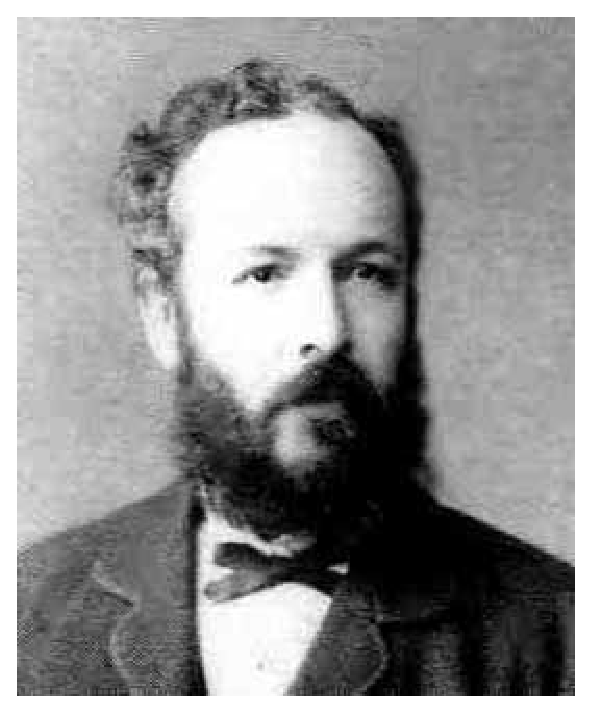
\includegraphics[width=3.5cm]{cantor.eps}
      \captionsetup{singlelinecheck=off,justification=raggedright}%,margin={1mm,0mm}
\caption{Cantor}
    \end{minipage}%
       \begin{minipage}[t]{.7\textwidth}
       \vspace{0pt}
       \hspace{8mm}
   En una carta a Dedekind, de fecha 29 de noviembre de 1873, Cantor afirmaba, sin incluir prueba alguna, que los racionales positivos y, m�s generalmente, el conjunto de las sucesiones finitas de enteros positivos, pod�a ponerse en correspondencia biyectiva con los enteros positivos, y preguntaba si eso mismo se pod�a hacer con los n�meros reales. Dedekind le respondi�, a vuelta de correo, que en su opini�n nada se opon�a a ello, y a�adi�, con demostraci�n incluida, que el conjunto de los n�meros algebraicos s� es biyectivo con el de los enteros positivos.
     \end{minipage}
      \end{center}
  \end{figure}\vspace*{-6mm}





\begin{definicion}
Los \emph{n�meros algebraicos} son n�meros, reales o complejos, que son ra�ces de alguna ecuaci�n polin�mica con coeficientes enteros. Por tanto, un n�mero real o complejo $x$ es algebraico si hay n�meros enteros $c_k\en\Z$, ($k=01,2,\dots n$) tal que $x$ satisface la ecuaci�n polin�mica
$$
c_0+c_1 x+c_2 x^2+\cdots+c_n x^n=0
$$
Los n�meros que no son algebraicos se llaman \emph{trascendentes}.
\end{definicion}
Todo n�mero racional es evidentemente algebraico, pero tambi�n lo son las ra�ces de cualquier orden de n�meros racionales positivos y muchos m�s. Intuitivamente, los n�meros algebraicos son los que pueden obtenerse a partir de los enteros por procedimientos algebraicos: suma, producto, cociente, divisi�n, ra�ces, iterados un n�mero finito cualquiera de veces. En ese sentido podemos decir que los n�meros algebraicos no est�n ``muy alejados'' de los enteros. Los n�meros trascendentes son justamente lo contrario: son n�meros irracionales ``muy alejados'' de los enteros.

Para facilitar la exposici�n que sigue voy a dar algunas definiciones de conceptos introducidos por Cantor a�os m�s tarde.
\begin{definicion}
Se dice que dos conjuntos $A$ y $B$ son \emph{equipotentes} si existe una aplicaci�n biyectiva de uno de ellos sobre el otro. Los conjuntos equipotentes al conjunto \N\ de los n�meros naturales se llaman conjuntos \emph{numerables}. \end{definicion}
Los conjuntos numerables son aquellos conjuntos cuyos elementos se pueden contar �aunque sean infinitos! El resultado, citado por Cantor, de que \Q\ es numerable, no deja de ser muy sorprendente y contrario a la intuici�n, pues si $r<s$ son n�meros racionales cualesquiera, entre ellos dos hay siempre infinitos n�meros racionales. Pese a ello, no hay m�s n�meros racionales que n�meros naturales.

Poco despu�s de las cartas citadas, Cantor logr� demostrar que el conjunto de los n�meros reales no es numerable. De aqu� se deduce enseguida que en todo intervalo de \R, hay infinitos n�meros trascendentes. Cantor public� estos resultados, el suyo y el de Dedekind, en un trabajo de tres p�ginas titulado \emph{Uber eine Eigenshaft des Inbegriffes aller reellen algebraischen Zahlen} (\emph{Sobre una propiedad del sistema de todos los n�meros algebraicos reales}) (1874). Es muy llamativo que el t�tulo de este trabajo, considerado como el nacimiento oficial de la teor�a de conjuntos, no haga referencia alguna al resultado que hoy consideramos como el principal: la no numerabilidad de \R. Adem�s la propia presentaci�n del trabajo elude destacar estos resultados. Posiblemente, Cantor tem�a la reacci�n que pudiera provocar un trabajo tan radicalmente innovador. Porque lo que �l hac�a era probar que en cualquier intervalo $[a,b]\subset\R$ con $a<b$ hay, en un sentido matem�tico preciso, m�s n�meros que todos los n�meros algebraicos juntos, de donde se deduc�a que en $[a,b]$ ten�a que haber n�meros trascendentes. Esta es una demostraci�n de \emph{existencia pura}, algo nuevo en las matem�ticas.

Demostrar que un n�mero concreto es trascendente es muy dif�cil. Era conocida la trascendencia del n�mero $\e$, demostrada por Charles Hermite en 1873, y Ferdinand Lindemann logr� probar la trascendencia de $\pi$ en 1882 (demostrando as� que el problema de la cuadratura del c�rculo no ten�a soluci�n).

Naturalmente, Cantor sab�a muy bien que hab�a descubierto una propiedad espec�fica del continuo: su no numerabilidad. Dispon�a ya de dos tipos de conjuntos infinitos: \N\ y \R, claramente \N\ ten�a un tama�o m�s peque�o que \R. Precisar esa idea de tama�o y elaborar una teor�a de comparaci�n de conjuntos infinitos es lo que hizo Cantor en los siguientes veinte a�os y, casi contra su voluntad, se vio llevado a desarrollar la teor�a de n�meros transfinitos y la teor�a de conjuntos como una disciplina matem�tica independiente.

En  1877, Cantor prob�, para su propia sorpresa, que los puntos del plano pod�an ponerse en correspondencia biyectiva con \R, y, m�s general, que los espacios $\R^n$ son todos ellos biyectivos a la recta real. Este resultado fue de los que m�s desconcierto provoc� entre los matem�ticos contempor�neos.

Cantor sigui� desarrollando sus ideas en una serie de seis trabajos publicados en los a�os 1878 a 1884. En 1883, en su trabajo \emph{Fundamentos de una teor�a general de conjuntos}, escribe:
\begin{quote}
\footnotesize{La presentaci�n de mis investigaciones hasta la fecha en teor�a de conjuntos, ha alcanzado un punto donde su progreso depende de una extensi�n del concepto de n�mero entero m�s all� de sus l�mites actuales. Esta extensi�n se�ala en una direcci�n que, por lo que yo s�, no ha sido investigada por nadie todav�a.

[\dots] Por atrevido que esto pueda parecer, tengo que expresar, no s�lo la esperanza, sino tambi�n la firme convicci�n de que esta extensi�n tendr� que ser considerada con el tiempo como absolutamente simple, adecuada y natural. Pero no se me oculta de ninguna manera el hecho de que en esta empresa me encuentro situado en una cierta oposici�n a concepciones muy extendidas acerca del infinito matem�tico, y a opiniones formuladas frecuentemente sobre la naturaleza del n�mero.}
\end{quote}
En este trabajo Cantor introduce los \emph{n�meros transfinitos} o \emph{cardinales transfinitos}. Por el mismo proceso que podemos abstraer la idea de n�mero $5$ como la clase de todos los conjuntos equipotentes a un conjunto cualquiera con cinco elementos, ${a,b,c,d,e}$, de la misma forma este proceso permite, dado un conjunto $M$, por doble abstracci�n de la naturaleza de sus elementos y del posible orden en que est�n dados, asociar a $M$ un objeto matem�tico, representado por $\sharp M$, que se llama \emph{su n�mero cardinal} o \emph{potencia}, que es el mismo para todos los conjuntos equipotentes a $M$. Cuando $M$ es finito, $\sharp M$ es el n�mero de elementos de $M$; la potencia de los conjuntos numerables (infinitos) la represent� Cantor por $\aleph_0$ ($\aleph$ es la primera letra del alfabeto hebreo, se pronuncia ``alef''); la potencia de la recta real y de cualquier intervalo de la misma, no vac�o y no reducido a un punto, se representa por $\bm{\mathfrak{c}}$ y se llama la \emph{potencia del continuo}.

Cantor define una relaci�n de orden entre n�meros cardinales: si $M$, $N$ son dos conjuntos, diremos que $\sharp M\preccurlyeq\sharp N$ si existe una biyecci�n de $M$ sobre \emph{una parte} de $N$. Si, adem�s, no existe ninguna biyecci�n entre ninguna parte de $M$ y la totalidad de $N$, se escribe  $\sharp M\prec\sharp N$. Con esta definici�n se tiene que $\aleph_0\prec\bm{\mathfrak{c}}$. Para n�meros cardinales finitos esta relaci�n de orden es la usual. La demostraci�n de que $\preccurlyeq$ es una relaci�n de orden entre n�meros cardinales est� muy lejos de ser f�cil. La dificultad estaba en probar la propiedad reflexiva, es decir, si $\sharp M\preccurlyeq\sharp N$ y tambi�n $\sharp N\preccurlyeq\sharp M$, entonces es $\sharp M=\sharp N$. Este resultado fue probado en 1898, y se conoce como teorema de Cantor - Bernstein. Se verifica, adem�s, que $\preccurlyeq$ es una relaci�n de orden total, es decir, dados conjuntos $M$ y $N$ se verifica alguna de las relaciones $\sharp M\preccurlyeq\sharp N$ o $\sharp N\preccurlyeq\sharp M$. La demostraci�n de este resultado exige usar el llamado axioma de Zermelo.

Todos esto est� muy bien, pero �cu�ntos n�meros cardinales infinitos hay? Hasta ahora solamente conocemos dos. Cantor ide� un procedimiento por el cual, dado un conjunto $M$, se puede construir un conjunto cuyo cardinal es estrictamente mayor. Para ello, defini� el conjunto $\mathcal{P}(M)$ como el conjunto cuyos elementos son todos los subconjuntos de $M$
$$
\mathcal{P}(M)=\set{A: A\subset M}
$$
Es f�cil probar que $\sharp M \prec\sharp \mathcal{P}(M)$. Suele escribirse $\sharp\mathcal{P}(M)=2^{\sharp M}$, igualdad que, para el caso de conjuntos finitos, es cierta.

Por tanto, los conjuntos
$$
\mathcal{P}(M), \mathcal{P}\big(\mathcal{P}(M)\big), \mathcal{P}\left( \mathcal{P}\big(\mathcal{P}(M)\big)\right)\dots
$$
tienen todos ellos distinto n�mero cardinal.

Las operaciones con n�meros transfinitos se definen con facilidad por medio de las correspondientes operaciones conjuntistas. Por ejemplo, el producto $\sharp M\cdot\sharp N$ es, por definici�n, igual a $\sharp(M\times N)$ donde $M\times N$ es el conjunto producto cartesiano de $M$ y $N$. An�logamente se define la suma $\sharp M + \sharp N$ como el n�mero cardinal de la uni�n disjunta de $M$ y $N$. Estas operaciones son asociativas, conmutativas y distributivas pero, para cardinales transfinitos se cumple que
$$
\sharp M + \sharp N=\sharp M \cdot\sharp N=\max\set{\sharp M, \sharp N}
$$
Esto es, la aritm�tica transfinita no responde a las reglas usuales de la aritm�tica finita. Pero esto no quiere decir que sea contradictoria, simplemente, es diferente.

El desarrollo de la teor�a de conjuntos condujo a algunas contradicciones, las llamadas \emph{paradojas de la teor�a de conjuntos}. Ello era debido al punto de vista ingenuo adoptado respecto a los conjuntos. Se pensaba que cualquier propiedad matem�tica, $P(x)$, defin�a su correspondiente conjunto, a saber, el formado por los elementos para los cuales dicha propiedad es verdadera. El propio Bolzano ten�a esta idea. Consideremos la siguiente propiedad $P(x)=x\notin x$ y definamos el conjunto $A=\set{x: P(x) \textrm{ es verdadera}}$. Entonces resulta que si $A\en A$ es porque $A\notin A$ y si $A\notin A$ debe ser $A\en A$. Una contradicci�n insalvable, conocida como la \emph{paradoja de Russell}. La soluci�n fue axiomatizar la teor�a de conjuntos para evitar que pudieran formularse paradojas como la anterior y, adem�s, restringir de alguna forma la existencia de conjuntos ``demasiado grandes''.

Considero que lo dicho hasta aqu� es suficiente para que tengas una idea del trabajo de Cantor. Este trabajo cambi� la forma de ver las matem�ticas y acab� por ser ampliamente aceptado. La visi�n que Cantor ten�a de las matem�ticas puras es muy hermosa; para �l, las matem�ticas puras son el reino de la libertad y las llamaba ``matem�ticas libres'', porque son una creaci�n de la libertad del esp�ritu humano cuyas �nicas limitaciones son la coherencia y la no contradicci�n.

\subsubsection{La no numerabilidad del continuo}
En esta secci�n final, vamos a probar la numerabilidad de \Q\ y la no numerabilidad de \R. As� mismo, estudiaremos algunos tipos de conjuntos densos y te propondr� algunos ejercicios interesantes.

Empezaremos demostrando un resultado que, por su aparente evidencia, parece que no precisa demostraci�n. Se trata de un resultado muy importante y muy �til y cuya demostraci�n me parece instructiva.
\begin{teorema}\label{maxminz}
a) Todo conjunto de n�meros enteros no vac�o y mayorado tiene m�ximo.

b) Todo conjunto de n�meros enteros no vac�o y minorado tiene m�nimo.
\end{teorema}
\dem La estrategia de la demostraci�n es obligada; para probar que un conjunto de n�meros reales no vac�o y mayorado tiene m�ximo, debemos probar que su supremo est� en el conjunto. Sea $E\subset\R$ no vac�o y mayorado. En virtud del principio del supremo, hay un n�mero $\beta\in\R$ que es el m�nimo mayorante de $E$. Puesto que $\beta-1<\beta$, debe haber alg�n $z\en E$ tal que $\beta-1<z\,$ y, claro est�, $z\leqslant \beta$. Supongamos que los elementos de $E$ son n�meros enteros,
$E\subset\Z$, y probemos que, en tal caso, debe ser $z=\beta$. Si fuera $z<\beta$ tendr�a que haber alg�n $w\en E$ tal que $z<w\leqslant \beta\,$ pero entonces el n�mero $\,w-z\,$ es un entero positivo tal que $w-z<1$ lo cual es contradictorio. En consecuencia $z=\beta\en E$ y $\beta$ es el m�ximo de $E$.

An�logamente se prueba que un conjunto no vac�o y minorado de enteros tiene m�nimo.\fin

Del teorema anterior se deducen dos importantes consecuencias.

\begin{teorema}[Principio de buena ordenaci�n de \N]
Todo conjunto no vac�o de n�meros naturales tiene m�nimo.
\end{teorema}

La siguiente propiedad, tambi�n consecuencia del teorema, nos dice que \N\ no est� mayorado en \R. Observa que es evidente que \N\ est� mayorado en \Q. Pero \R\ tiene muchos m�s elementos (much�simos m�s, como enseguida veremos) que \Q; �qui�n te asegura que, en la ampliaci�n de \Q\ a \R, no se han colado n�meros irracionales m�s grandes que cualquier natural? De eso se trata.

\begin{teorema}[Propiedad arquimediana]\label{th:arquimediana}
Dado cualquier n�mero real se verifica que hay n�meros naturales mayores que �l.
\end{teorema}
\dem Como \N\ no tiene m�ximo, el teorema (\ref{maxminz}) implica que \N\ no puede estar mayorado en \R, por tanto, dado $x\!\in\!\R$, tiene que haber alg�n $n\en\N$ tal que $n>x\,$.\fin

La propiedad arquimediana del orden de \R\ proh�be la existencia de cantidades infinitesimales, es decir, de n�meros positivos pero ``tan peque�os'' que al multiplicarlos por cualquier n�mero natural el producto segu�a siendo ``muy peque�o''. Convenz�monos de que tales ``infinit�simos'', si es que los hay, no pueden ser n�meros reales. En efecto, si $\,x,y\,$ son n�meros reales positivos, la propiedad arquimediana del orden de \R\ nos dice que tiene haber alg�n $n\en\N$ tal que $\,n>y/x$ y, por tanto, $nx>y$. En consecuencia, por ``peque�o'' que sea el n�mero real $x\!>\!0$ y por ``muy grande'' que sea el n�mero real $y\!>\!0$, siempre hay m�ltiplos naturales de $x$  mayores que $y$.

\begin{definicion}
Se dice que un conjunto $E\subset\R$ es denso en \R, si en todo intervalo abierto no vac�o hay puntos de $E$. Equivalentemente, si dados $x,y\en\R$ con $x<y$ hay alg�n $z\en E$ tal que $x<z<y$.
\end{definicion}
\begin{proposicion}\label{prop:densidad}
\begin{enumerate}[a)]
\item El conjunto de los n�meros racionales es denso en \R.
\item El conjunto de los n�meros irracionales es denso en \R.
\end{enumerate}
\end{proposicion}
\dem \emph{a)} Supongamos que $x,y\en\R$ con $x<y$. La idea es tomar una unidad racional de medida, $u$, en la recta que sea menor que $y-x$, pues entonces es claro que un m�ltiplo apropiado, $m u$, de $u$ estar� comprendido entre $x$ e $y$. Hay muchas posibilidades, se trata de elegir $u$ y $m$ con alg�n criterio que nos permita probar que $x<mu<y$. Los n�meros m�s sencillos que podemos tomar para $u$ son los de la forma $1/n$, donde $n\en\N$, con la condici�n $1/n<y-x$, esto es, $n>1/(y-x)$. Parece razonable tomar el menor $n$ que cumpla dicha desigualdad. Sea, pues:
$$
q=\min\set{n\en\N: n>1/(y-x)}
$$
Ahora se trata de tomar un m�ltiplo de $u=1/q$ que exceda a $x$, pero no demasiado. Se impone la elecci�n:
$$
p=\min\set{m\en\Z: m > q x}
$$
Tenemos que:
$$
x<\frac{p}{\ q\ }=\frac{p-1}{q}+\frac{1}{q}<x+(y-x)=y
$$
Lo que concluye la demostraci�n. Observa que en las definiciones de $q$ y de $p$ se usan los resultados que acabamos de ver.

\emph{b)} Supongamos que $x,y\en\R$ con $x<y$. Por lo ya probado, existe $\,r\en\Q\,$ tal que $$x-\sqrt{2}<r<y-\sqrt{2},$$ lo que implica que $\,x<r+\sqrt{2}<y$. Puesto que, $\sqrt{2}\,$ es irracional y $\,r\en\Q$, se sigue que $\,r+\sqrt{2}\,$ es irracional y concluimos que \irr\ es denso en \R.\fin

Este resultado nos dice que los n�meros racionales y los irracionales est�n repartidos de manera que entre dos racionales o entre dos irracionales siempre hay infinitos racionales e infinitos irracionales. Son dos conjuntos muy grandes, pero uno de ellos es much�simo m�s grande que el otro.

Hemos definido antes un conjunto numerable como aqu�l que es equipotente a \N; es conveniente incluir tambi�n entre los conjuntos numerables a los conjuntos finitos pues los elementos de un conjunto finito se pueden contar. Estas dos posibilidades pueden resumirse en el hecho de que exista una aplicaci�n \emph{inyectiva} del conjunto en \N. Por convenio, se admite que el conjunto vac�o es numerable.

\begin{definicion}
Un conjunto se llama numerable si es vac�o o si existe una aplicaci�n inyectiva de �l en el conjunto de los enteros positivos.
\end{definicion}
Realmente esta definici�n lo que nos da es cierta libertad para probar que un conjunto es numerable; de hecho, se verifica el siguiente resultado.
\begin{proposicion}
Un conjunto no vac�o es numerable si, y s�lo si, es finito o es equipotente a \N.
\end{proposicion}
El siguiente resultado es muy �til y f�cil de entender.
\begin{proposicion}\label{criterioenumera}
Un conjunto no vac�o $\,A\,$ es numerable si, y s�lo si, hay una aplicaci�n sobreyectiva de \N\ sobre $\,A$.
\end{proposicion}
\dem Sea $\,f:\N\rightarrow A\,$ una aplicaci�n sobreyectiva. Para cada elemento $\,a\en A\,$ el conjunto $\,\{n\en\N:f(n)=a\}\,$ no es vac�o por lo que podemos definir, haciendo uso del principio de buena ordenaci�n,
una aplicaci�n $\,g:A\rightarrow\N\,$ por:
$$
g(a)=\min \{n\en\N:f(n)=a\} \qquad \textrm{para todo }\  a\en A
$$
Con ello se tiene que $\,f(g(a))=a$ para todo $a\en A\,$ lo que implica que $\,g\,$ es inyectiva y por tanto que $\,A\,$ es numerable.

La afirmaci�n rec�proca es consecuencia de la proposici�n anterior. \fin

Aunque el conjunto $\N\times\N$ parece mucho m�s grande que \N; de hecho no es as�. Podemos contar con facilidad los elementos de $\N\times\N$ siguiendo el camino que se sugiere (habr�a que prolongarlo hacia arriba y hacia la derecha) en la figura (\ref{fig:contandonn}).

\begin{proposicion}
$\N\times\N$ es equipotente a \N.
\end{proposicion}
\dem\footnote{En el ejercicio (\ref{biyeccionnn}) se define una biyecci�n de $\N\times\N$ sobre \N} La aplicaci�n \mbox{$\ff\!:\!\N\!\times\!\N\!\rightarrow\!\N$} dada por ${\dis \,\ff(p,q)=2^{p}3^{q}}$ para todo $(p,q)\en\N\times\N$, es inyectiva. En consecuencia $\N\times\N$ es numerable y como es infinito concluimos que
es equipotente a \N.\fin

El siguiente resultado nos dice que si hacemos la uni�n de una ``cantidad numerable'' de conjuntos numerables obtenemos un conjunto que sigue siendo numerable. El enunciado del teorema precisa estas ideas.
\begin{teorema}
Sea $\,B\,$ un conjunto numerable no vac�o. Supongamos que para cada $\,x\en B\,$ tenemos un conjunto numerable no vac�o $\,A_{x}$. Se verifica entonces que el conjunto $\dis{\,{\mathcal A} = \bigcup_{x\in B}A_{x}}$ es numerable.
\end{teorema}


\begin{figure}[ht]
\centering
\begin{pspicture}(0,0)(10,10)%
\psset{labelsep=2pt, arrowscale=1.4,xunit=1.2cm}
\psaxes[linewidth=.6pt]{->}(0,0)(-.2,-.2)(10,10)
\multido{\in=1+1}{9}{%
\multido{\im=1+1}{9}{%
\uput[u](\in,\im){\scalefont{.6}$(\im,\in)$}%
\qdisk(\in,\im){1.2pt}}}
\psline[linewidth=.4pt,ArrowInside=->]{->}(1,1)(2,1)(1,2)(1,3)(2,2)(3,1)(4,1)(3,2)(2,3)(1,4)(1,5)(2,4)(3,3)(4,2)(5,1)(6,1)(5,2)(4,3)(3,4)(2,5)(1,6)(1,7)(2,6)(3,5)(4,4)(5,3)(6,2)(7,1)(8,1)(7,2)(6,3)(5,4)(4,5)(3,6)(2,7)(1,8)(1,9)(2,8)(3,7)(4,6)(5,5)(6,4)(7,3)(8,2)(9,1)(9,2)(8,3)(7,4)(6,5)(5,6)(4,7)(3,8)(2,9)(3,9)(4,8)(5,7)(6,6)(7,5)(8,4)(9,3)(9,4)(8,5)(7,6)(6,7)(5,8)(4,9)(5,9)(6,8)(7,7)(8,6)(9,5)(9,6)(8,7)(7,8)(6,9)(7,9)(8,8)(9,7)(9,8)(8,9)(9,9)
\end{pspicture}\vspace*{3mm}
\caption{Contando $\N\times\N$}\label{fig:contandonn}
\end{figure}

\dem Es suficiente probar que hay una aplicaci�n sobreyectiva de $\N\times\N$ sobre $\,\mathcal A$. Por ser $\,B\,$ numerable hay una aplicaci�n sobreyectiva $\,\phi :\N\rightarrow B$. Para cada $\,x\en B$, por ser $\,A_{x}$ numerable, hay una aplicaci�n sobreyectiva $\,F_{x}:\N\rightarrow A_{x}$. Es muy f�cil comprobar ahora que la aplicaci�n $\,G:\N\times\N\rightarrow{\mathcal A}\,$ definida por $G(m,n)=F_{\phi(m)}(n)$ para todo $(m,n)\en\N\times\N$, es
sobreyectiva. \fin

Puede que el siguiente diagrama sea m�s claro y directo que la demostraci�n anterior. Podemos suponer que $B=\N$, con lo que  $\dis{\,{\mathcal A} = \bigcup_{n\in\N}A_{n}}$. Como $A_n$ es numerable, podemos escribir sus elementos como una sucesi�n:
$$
A_n=\set{a_{mn}:m\en\N}=\set{a_{1n},a_{2n},a_{3n},\dots,a_{mn},\dots}
$$
El conjunto $\mathcal{A}$ podemos representarlo como una matriz (ver figura (\ref{fig:unionnumerable})), y contar sus elementos de forma parecida a como lo hemos hecho antes con $\N\times\N$.

\begin{figure}[ht]
\centering
\begin{pspicture}(0,0)(8.5,8.5)%
\psset{labelsep=2pt, arrowscale=1.4,unit=.85cm}
%\psaxes[linewidth=.6pt]{->}(0,0)(-.2,-.2)(10,10)
\multido{\in=1+1}{9}{%
\multido{\im=1+1}{9}{%
\uput[u](\in,\im){\scalefont{.7}$a_{\im\in}$}}}
\psline[linewidth=.3pt,ArrowInside=->,linestyle=dashed,linearc=.1]{->}(1,1)(2,1)(1,2)(1,3)(2,2)(3,1)(4,1)(3,2)(2,3)(1,4)(1,5)(2,4)(3,3)(4,2)(5,1)(6,1)(5,2)(4,3)(3,4)(2,5)(1,6)(1,7)(2,6)(3,5)(4,4)(5,3)(6,2)(7,1)(8,1)(7,2)(6,3)(5,4)(4,5)(3,6)(2,7)(1,8)(1,9)(2,8)(3,7)(4,6)(5,5)(6,4)(7,3)(8,2)(9,1)(9,2)(8,3)(7,4)(6,5)(5,6)(4,7)(3,8)(2,9)(3,9)(4,8)(5,7)(6,6)(7,5)(8,4)(9,3)(9,4)(8,5)(7,6)(6,7)(5,8)(4,9)(5,9)(6,8)(7,7)(8,6)(9,5)(9,6)(8,7)(7,8)(6,9)(7,9)(8,8)(9,7)(9,8)(8,9)(9,9)
\end{pspicture}\vspace*{-3mm}
\caption{Uni�n numerable}\label{fig:unionnumerable}
\end{figure}

\begin{teorema}
El conjunto de los n�meros racionales es numerable.
\end{teorema}
\dem
Puesto que la aplicaci�n $\,\ff:\Z\rightarrow\N\,$ definida por:
$$
\ff(n)=\left\{ \begin{array}{ll}
                2n & \mbox{si \, $n>0$} \\
                1-2n & \mbox{si \, $n\leqslant 0$}
                \end{array}
\right. $$ es una biyecci�n, y para cada $\,m\in\Z$ el conjunto:
$$
A_{m}=\left\{ \frac{m}{p}\,:\,p\in\N \right\}
$$
es numerable, se sigue del resultado anterior que ${\dis \,\Q=\bigcup_{m\in\Z}\!A_{m}}$  es numerable. \fin

Por ser \Q\ numerable infinito se verifica que \Q\ es equipotente a \N, es decir, existen biyecciones de \N\ sobre \Q. Hemos respondido en parte a nuestra pregunta inicial: hay tantos n�meros racionales como n�meros naturales. Nos falta todav�a dar alguna informaci�n del tama�o de \irr.

\begin{teorema}[Principio de los intervalos encajados] Para cada n�mero natural $\,n\,$ sea $\,I_{n}=[a_{n},b_{n}]\,$ un intervalo cerrado no vac�o y supongamos que para todo $n\in\N$ es $\,I_{n+1}\subset I_{n}$. Se verifica entonces que:

\noindent i)${\dis \ \ \alpha=\sup \{a_{n}:n\in\N\} \leqslant \beta=\inf
\{b_{n}:n\in\N\}}$.

\noindent ii) ${\dis \ \bigcap_{n\in\N}\!I_{n}=[\alpha,\beta]}$.

\noindent En particular, el conjunto ${\dis \,\bigcap_{n\in\N}\!I_{n}}$ no es vac�o.
\end{teorema}
\dem \emph{i)} Las hip�tesis $\vac\!\neq\! I_{n+1}\!\subset\!I_{n}$, implican que $a_{n}\leqslant a_{n+1}\leqslant b_{n+1}\leqslant b_{n}$ para todo $n\in\N$. Deducimos que las aplicaciones $\,n\mapsto a_{n}$ y $\,n\mapsto -b_{n}$, son crecientes, esto es, $\,a_{n}\leqslant a_{m},\ b_{m}\leqslant b_{n}$ siempre que $\,n<m$. Ahora, dados $\,p,q\in\N$ y poniendo $\,k=\max\{p,q\}$, tenemos que $\,a_{p}\leqslant a_{k}\leqslant b_{k}\leqslant b_{q}$. Hemos obtenido as� que cualesquiera sean los n�meros naturales $\,p,q\,$ es $\,a_{p}\leqslant b_{q}$. Luego todo elemento de $\,B=\{b_{n}:n\in\N\}\,$ es  mayorante de $\,A=\{a_{n}:n\in\N\}\,$ y por tanto $\,\alpha=\sup A \leqslant b_{n}$ para todo $n\in\N$. Lo cual, a su vez, nos dice que $\,\alpha\,$ es un minorante de $\,B\,$ y por tanto concluimos que $\,\alpha\leqslant \beta=\inf B$.

\emph{ii)} Es consecuencia de que ${\dis x\in\!\!\bigcap_{n\in\N}\!I_{n}}$ equivale a que $a_{n}\leqslant x \leqslant b_{n}$ para todo $n\in\N$, lo que equivale a que $\alpha\leqslant x\leqslant\beta$, es decir $x\in [\alpha,\beta]$.\fin

\begin{teorema}
Dados dos n�meros reales $\,a<b\,$ se verifica que el intervalo $[a,b]$ no es numerable.
\end{teorema}
\dem Si $[a,b]$ fuera numerable tendr�a que ser equipotente a \N. Veamos que esto no puede ocurrir. Supongamos que $\,\ff :\N\rightarrow [a,b]\,$ es una biyecci�n de \N\ sobre $[a,b]$. En particular $\,\ff\,$ es sobreyectiva por lo que deber� ser $\,[a,b]=\{\ff(n):n\in\N\}$. Obtendremos una contradicci�n probando que tiene que existir alg�n elemento $\,z\in [a,b]\,$ tal que $\,z\not\in \{\ff(n):n\in\N\}$.

Para ello se procede de la siguiente forma. Dividimos el intervalo $[a,b]$ en tres intervalos cerrados de igual longitud:
$$
\left [ a,a+\frac{b-a}{3}\right ],\ \ \left [ a+\frac{b-a}{3},b-\frac{b-a}{3}\right ],\ \
\left [b-\frac{b-a}{3},b \right ]
$$
y llamamos $\,I_{1}$ al primero de ellos (es decir el que est� m�s a la izquierda) que no contiene a $\,\ff(1)$. Dividamos ahora el intervalo $\,I_{1}$ en tres intervalos cerrados de igual longitud y llamemos $\,I_{2}$ al primero de ellos que no contiene a $\,\ff(2)$.

Este proceso puede ``continuarse
indefinidamente'' pues, supuesto que $\,n\in\N,\,n\geqslant 2$, y que tenemos intervalos cerrados de longitud {\em positiva\/} $I_{k},\ 1\leqslant k\leqslant n,$ tales que $I_{k+1}\subset I_{k}$ para $\,1\leqslant k\leqslant n-1$, y $\ff(k)\not\in I_{k}$ para $\,1\leqslant k\leqslant n$, dividimos el intervalo $\,I_{n}$ en tres intervalos cerrados de igual longitud y llamamos $\,I_{n+1}$ al primero de ellos que no contiene a $\,\ff(n+1)$. De esta forma para cada $\,n\in\N$ tenemos un intervalo cerrado $\,I_{n}$ no vac�o verific�ndose que $\,I_{n+1}\subset I_{n}$ y $\ff(n)\not\in I_{n}$ para todo $n\in\N$. El principio de los intervalos encajados nos dice que hay alg�n n�mero real $\,z\,$ que est\'a en {\em todos\/} los $\,I_{n}$. Por tanto, cualquiera sea $\,n\in\N$, por ser $\,z\in I_{n}$ y $\,\ff(n)\not\in I_{n}$, se tiene necesariamente que $\,z\neq\ff(n)$, esto es, $z\not\in\{\ff(n):n\in\N\}$ pero,
evidentemente, $z\in [a,b]$. \fin

�Te recuerda algo la demostraci�n anterior? �Quiz�s a la divisibilidad infinita del continuo? Pues claro, lo que estamos haciendo es dividir infinitas veces un segmento (el prototipo de \emph{continuo}). Lo que nos dice este resultado es que, aunque lo dividamos en un infinito actual de partes, siempre nos quedar�n puntos que no habremos tocado. Arist�teles afirmaba que un continuo puede dividirse en cualquier parte pero no en todas partes: hay que darle la raz�n en este punto.

\begin{teorema}
\R\ y \irr\ son conjuntos no numerables.
\end{teorema}
\dem Evidentemente todo subconjunto de un conjunto numerable tambi�n es numerable. Como acabamos de ver que hay subconjuntos de \R\ que no son numerables deducimos que \R\ no es numerable. Puesto que $\,\R=\Q\cup(\irr)\,$ y sabemos que \Q\ es numerable y \R\ no lo es, deducimos que \irr\  no es numerable. \fin

El teorema anterior demuestra no solamente que \irr\ no es vac�o sino
que ``hay muchos m�s n�meros irracionales que racionales'' pues
mientras que podemos enumerar los racionales no podemos hacer lo mismo
con los irracionales ya que no hay biyecciones de \N\ sobre \irr.

Deducimos tambi�n la siguiente estrategia \emph{para probar que un conjunto $A\!\subset\!\R$ no es vac�o es suficiente probar que su complemento $\,\R\!\setminus\! A\,$ es numerable} (!con lo cual, de hecho, estamos probando que $\,A\,$ es infinito no numerable!).

\begin{ejercicios propuestos}
\propuesto\label{biyeccionnn} Prueba que la aplicaci�n
$\,F:\N\times\N\rightarrow\N\,$ dada por: $$ f(m,n)=
n+\frac{(m+n-2)(m+n-1)}{2}\ \ \ {\mbox{\rm para todo}}\
(m,n)\in\N\times\N $$ es una biyecci�n.

Sugerencias: para cada $\,p\in\N$ definamos: $$ \ff(p)=\max\left\{q\in\N:q<\sqrt{2p+\frac{1}{4}}+\frac{1}{2}\right\} $$ Observa que $\ff(p)$ es un n�mero natural mayor o igual que $2$. Prueba que para todo $\, p\in\N$ se verifica: $$ \frac{(\ff(p)-2)(\ff(p)-1)}{2}<p\leqslant \frac{(\ff(p)-1)\ff(p)}{2} \ \
\ \ \ (*) $$ Definamos ahora: $$ h(p)=p-\frac{(\ff(p)-2)(\ff(p)-1)}{4},\quad {\mbox{\rm
para todo}}\  p\in\N $$ Justifica, teniendo en cuenta $(*)$, que $\,h(p)\in\N$ y $\ff(p)-h(p)\geqslant 1.$

Comprueba finalmente que, $\,p=F(\ff(p)-h(p),h(p))$, para cada $\,p\in\N.$

\propuesto Sea \func{f}{[a,b]} creciente. Para cada $\,\alpha\in ]a,b[$
definamos: $$ \omega(f,\alpha)=\inf\{f(t):\alpha<t\leqslant b\}-\sup\{f(s):a\leqslant
s<\alpha\} $$ Prueba que:

i) $\,\omega(f,\alpha)\geqslant 0$ y $\omega(f,\alpha)=0$ si, y s�lo si, $f$ es continua en $\alpha$.

ii) Si $\,a<\alpha_{1}<\alpha_{2}<\cdots<\alpha_{p}<b$, entonces: $$
\omega(f,\alpha_{1})+\omega(f,\alpha_{2})+\cdots+\omega(f,\alpha_{p})\leqslant f(b)-f(a)
$$
iii) Para cada $\,n\in\N$ el conjunto $\,S_{n}=\{\alpha\in ]a,b[\,:\, \omega(f,\alpha)\geqslant 1/n\}\,$ es finito.

iv) El conjunto $\,S=\{\alpha\in ]a,b[\,:\, \omega(f,\alpha)>0\}\,$ de las discontinuidades de $f$ es numerable.

Muestra con un ejemplo que el conjunto $\,S\,$ puede ser infinito.

\propuesto \label{numeroejercicio}Prueba que el conjunto de los n�meros algebraicos es numerable.
\end{ejercicios propuestos}

Para terminar, recordemos que los poetas tambi�n se interesan por el infinito y lo llaman \emph{amor} y tambi�n \emph{deseo}.
\begin{quote}
\small{\emph{This is the monstruosity in love, lady,\\ that the will
is infinite \\ and the execution confined, \\ that the
desire is boundless\\ and the act a slave to limit.}}\newline
\footnotesize{Shakespeare - Troilus and Cressida}
\end{quote}










\chapter{Derivadas}
\vspace*{-1cm}
\begin{flushright}
{\small \textit{El arte de nombrar y de medir con exactitud aquello  \\ de lo que ni siquiera puede concebirse su existencia.} \\  Voltaire}
\end{flushright}\vspace*{-1mm}
\section{Introducci�n}\vspace*{-1mm}
Los or�genes del C�lculo estuvieron motivados por el deseo de resolver diversos problemas vinculados al movimiento de los cuerpos, as� como problemas de tipo geom�trico de importancia en �ptica y problemas de c�lculo de valores m�ximos y m�nimos de una funci�n dada. Simplificando, podemos destacar dos problemas principales:
\begin{itemize}
\item[$\bullet$] Determinar la tangente a una curva en un punto (el problema de las tangentes).
\item[$\bullet$] Determinar el �rea encerrada por una curva (el problema de las cuadraturas).
\end{itemize}
Son los conceptos de derivada e integral, respectivamente, los que permiten resolver satisfactoriamente dichos problemas. Mientras que el concepto de integral tiene sus ra�ces en la antig�edad cl�sica, la otra idea fundamental del C�lculo, la derivada, no se formul� hasta el siglo XVII. Fue el descubrimiento efectuado por Sir Isaac Newton (1642 - 1727) y Gottfried Wilhelm Leibniz (1646 - 1716) de la relaci�n entre estas dos ideas, tan dispares en apariencia, lo que inici� el magn�fico desarrollo del C�lculo. Si bien los trabajos de Newton y Leibniz son decisivos por sus aportaciones e influencia, no hay que olvidar que ellos son el punto culminante de un largo proceso en el que han participado cient�ficos de la talla de Johannes Kepler (1571 - 1630), Ren� Descartes (1596 - 1650), Pierre de Fermat (1601 - 1665), John Wallis (1616 -1703) e Isaac Barrow (1630 - 1677) entre otros.

\section{Concepto de derivada. Interpretaci�n f�sica y geom�trica}
Para entender los resultados del C�lculo diferencial es necesario, antes que nada, comprender la idea b�sica del mismo: el concepto de derivada. La derivada de una funci�n puede interpretarse geom�tricamente como la pendiente de una curva, y f�sicamente como una raz�n ``instant�nea'' de cambio.
\subsection{Tangente a una curva}
En la primera mitad del siglo XVII no se conoc�an m�todos generales para calcular la tangente a una curva en un punto de la misma. Este problema se presentaba con frecuencia en mec�nica, en �ptica y en geometr�a, y generalmente se resolv�a, de forma geom�trica, con t�cnicas adaptadas a cada caso particular. La dificultad est� en que, siendo la tangente una recta, se precisa conocer dos puntos de la misma, o bien un punto y su pendiente, para poderla determinar.

Supongamos que queremos hallar la tangente a una curva de ecuaci�n cartesiana $y= f(x)$ en el punto $(a,f(a))$. La estrategia, usada primero por Pierre de Fermat y m�s tarde por Newton, consiste en aproximar la tangente por rectas secantes cuyas pendientes s� pueden calcularse directamente. En particular, consideremos la recta que une el punto $(a,f(a))$ con un punto cercano, $(x,f(x))$, de la gr�fica de $f$. Esta recta se llama una secante (recta que corta a la curva, pero no es tangente a la curva). La pendiente de esta secante es:
$$
\frac{f(x)-f(a)}{x-a}
$$
dicho n�mero suele llamarse \emph{cociente incremental de $f$ en $a$}.

\begin{floatingfigure}{75mm}
\flushleft
\begin{pspicture}(1,-.2)(6,4)
\psset{algebraic,xunit=1.25cm,yunit=.7cm,labelsep=2pt}
\psaxes[labels=none,ticks=none,linewidth=.5pt,arrowscale=1.4]{->}(1.5,0)(1.3,-.2)(6,7)
\psplot[plotstyle=curve,linewidth=.7pt]{2}{5.3}{x^2-6*x+10}
\psplot[linewidth=.5pt]{3.2}{5.5}{-7.5+2.5*x}
\psline[linewidth=.4pt](3.5,1.25)(5,1.25)(5,5)
\uput[ul](3.5,1.25){\scalefont{.7}$(a,f(a))$}
\uput[l](5,5){\scalefont{.7}$(x,f(x))$}
\uput[r](5,3.15){\scalefont{.7}$f(x)-f(a)$}
\uput[d](4.5,1.25){\scalefont{.7}$x-a$}
\end{pspicture}
\caption{Secante}
\end{floatingfigure}

Observa que una secante es una buena aproximaci�n de la tangente, siempre que el punto $(x,f(x))$ est� pr�ximo a $(a,f(a))$. Estas consideraciones llevan a \emph{definir la tangente a la gr�fica de $f$ en el punto $(a,f(a))$  como la recta que pasa por dicho punto y cuya pendiente es igual al l�mite}:
$$
\lim_{x\to a}\frac{f(x)-f(a)}{x-a}
$$
supuesto, claro est�, que dicho l�mite exista.
\subsection{Raz�n de cambio puntual y velocidad instant�nea}
Muchas leyes de la F�sica, la Qu�mica, la Biolog�a o la Econom�a, son funciones que relacionan una variable ``dependiente'' $y$ con otra variable ``independiente'' $x$, lo que suele escribirse en la forma $y=f(x)$. Si la variable independiente cambia de un valor inicial $a$ a otro $x$, la variable $y$ lo hace de $f(a)$ a $f(x)$. La \emph{raz�n de cambio promedio de $y=f(x)$ con respecto a $x$ en el intervalo $[a,x]$}
es:
$$
\textrm{Raz�n de cambio promedio\ }= \frac{f(x)-f(a)}{x-a}
$$
Con frecuencia interesa considerar la raz�n de cambio en intervalos cada vez m�s peque�os. Esto lleva a definir lo que podemos llamar ``\emph{raz�n de cambio puntual de $y=f(x)$ con respecto a $x$ en el punto $a$}'' como:
$$
\lim_{x\to a}\frac{f(x)-f(a)}{x-a}.
$$
El ejemplo m�s conocido de esto que decimos es el de un m�vil que se mueve a lo largo de una recta sobre la cual hemos elegido un origen. Sea $s(t)$ la posici�n del m�vil en el tiempo $t$, es decir, la distancia con signo del m�vil al origen en el tiempo $t$. La raz�n de cambio promedio tiene en este caso una interpretaci�n f�sica natural:
$$
\frac{s(a+h)-s(a)}{h}
$$
Es la \emph{velocidad media} del m�vil en el intervalo de tiempo comprendido entre $a$ y $a+h$. Parece intuitivo que, en cada instante, el m�vil se mueve con una determinada \emph{velocidad instant�nea}. Pero no hay manera de medir directamente una velocidad instant�nea; un instante quiere decir una posici�n en la recta: la velocidad instant�nea del m�vil para $t=a$ es la velocidad que tiene cuando est� en la posici�n $s(a)$. La velocidad instant�nea es una abstracci�n de un caracter�stica f�sica del movimiento, pero no es una magnitud que podamos observar directamente. La �nica definici�n razonable de velocidad instant�nea es como la raz�n de cambio puntual:
$$
\lim_{h\to 0}\frac{s(a+h)-s(a)}{h}
$$

\noindent\textbf{Notaci�n}.\ En lo que sigue usaremos las letras $I$, $J$ para representar intervalos no vac�os de n�meros reales.

\begin{definicion}\label{def:derivada} Se dice que una funci�n \func{f}{I}\ es \textbf{derivable en un punto $a\en I$}, si existe el l�mite:
$$
\lim_{x\to a}\frac{f(x)-f(a)}{x-a}.
$$
Expl�citamente, $f$ es derivable en $a$ si hay un n�mero $L\en\R$ verificando que para cada n�mero $\varepsilon >0$ existe alg�n n�mero $\delta >0$ tal que para todo $x\in I$ con $x\neq a$ y \mbox{$\mid x-a\mid<\delta $} se tiene que:
$$\left| \frac{f(x)-f(a)}{x-a}\ -\ L \right| \leqslant \varepsilon.$$
Dicho n�mero $L$ se llama \textbf{derivada de $f$ en $a$} y lo
representaremos por $f\tl(a)$ (notaci�n debida a Lagrange).
\end{definicion}

La notaci�n de Lagrange tiene la gran ventaja de poner de manifiesto que al aplicar la operaci�n de derivaci�n a una funci�n obtenemos una nueva funci�n, que est� definida en todos los puntos donde la funci�n dada sea derivable. Es usual considerar funciones derivadas definidas en intervalos.

\begin{definicion}
Dada una funci�n $f:I\rightarrow \R$ derivable en todo punto de $I$, la \textbf{funci�n derivada} de $f$ es la funci�n $f\tl:I\rightarrow \R$ que a cada punto $x\in I$ hace corresponder la derivada de $f$ en dicho punto.
\end{definicion}

\begin{observaciones}\label{ob:propiedadlocalderivada}
\noindent\textbf{i)}\ El l�mite $\ {\displaystyle \lim_{x\to a}\frac{f(x)-f(a)}{x-a}}$ se
puede escribir tambi�n de la forma $\ {\displaystyle \lim_{h\to 0}\frac{f(a+h)-f(a)}{h}.}$

\noindent\textbf{ii)}\ La derivabilidad de $f$ en un punto $ a\in I$ es una \emph{propiedad local}, depende solamente del comportamiento de $f$ en los puntos de $I$ pr�ximos al punto $a$. Concretamente, si $J$ es cualquier \emph{intervalo abierto} que contiene el punto $a$, se verifica que $f$ es derivable en $a$ si, y s�lo si, la funci�n restricci�n $f_{|I\cap J}$ es derivable en $a$ y, por supuesto, en tal caso ambas funciones tienen la misma derivada en $a$.
\end{observaciones}

\noindent\textbf{La notaci�n diferencial de Leibniz.}\ La notaci�n $\dfrac{\df{f(x)}}{\df{x}}$ para representar la derivada de $f$ en $x$ es debida a Leibniz.

Leibniz interpretaba ese s�mbolo como un ``cociente diferencial'' pues �l lo entend�a as�: como un cociente de cantidades infinitesimales, y lo manejaba como un cociente; por ejemplo, se puede multiplicar o dividir, seg�n convenga, por $\df{x}$ o $\df{f(x)}$. En el cap�tulo 5 hemos visto los problemas que planteaba el uso de cantidades infinitesimales, y c�mo, finalmente, a partir del �ltimo tercio del siglo XIX, fueron totalmente abandonadas. Por eso, la  interpretaci�n de Leibniz de la derivada, aunque intuitiva, no es la que se sigue en la gran mayor�a de los cursos de c�lculo\footnote{Aunque s� en los cursos de An�lisis No Est�ndar basados en los hiperreales de A. Robinson.}.

A pesar de lo dicho, es frecuente, sobre todo en libros de ingenier�a, usar la notaci�n de Leibniz y manejarla como �l lo hac�a. Creo que esto es �til porque la notaci�n de Leibniz tiene una gran fuerza heur�stica, y no debe presentar ning�n problema, siempre que no acabes creyendo que una derivada, tal como la hemos definido, es un cociente de infinit�simos. Y siempre que dicha notaci�n se use como un mero simbolismo y no se hagan demostraciones apoyadas en su supuesta significaci�n.

Una dificultad de la notaci�n de Leibniz es que no es c�moda para representar la derivada en un punto concreto. Podemos entender que $\dfrac{\df{f(x)}}{\df{x}}$ es la funci�n derivada $f\tl(x)$, pero �c�mo indicamos la derivada en punto concreto $a$? Las notaciones $\dfrac{\df{f(a)}}{\df{x}}$ y $\dfrac{\df{f(x)}}{\df{x}}(a)$ son confusas. Lo que suele hacerse es escribir:
$$
\left.\dfrac{\df{f(x)}}{\df{x}}\right|_{x=a}
$$
que, realmente, es una notaci�n inc�moda. Una posible mejora ser�a escribir $\dfrac{\df{f}}{\df{x}}(x)$ para representar $f\tl(x)$, en cuyo caso $\dfrac{\df{f}}{\df{x}}(a)$ indicar�a $f\tl(a)$.

La verdad es que la mayor�a de los libros de ingenier�a que usan estas notaciones lo hacen sin preocuparse mucho por su significado, y esa es una causa importante de que muchas veces no se entienda bien lo que escriben. Las notaciones son importantes y hay que manejarlas cuidadosamente. Y todav�a m�s, cuando una notaci�n se supone que tiene un significado casi m�gico, y que por su fuerza simb�lica ella sola, por s� misma, proporciona demostraciones. Volveremos a considerar este asunto m�s adelante.

\begin{definicion}
Supuesto que $f$ es derivable en $a$, la recta de ecuaci�n cartesiana:
$$
y=f(a)+f\tl(a)(x-a)
$$
se llama \textbf{recta tangente} a la gr�fica de $f$ en el punto $(a,f(a))$, y tambi�n recta tangente a $f$ en $x=a$.

Cuando $f\tl(a)\neq 0$, la recta de ecuaci�n:
$$
y=f(a)-\dfrac{1}{f\tl(a)}(x-a)
$$
es la \textbf{recta normal} a la gr�fica de $f$ en el punto $(a,f(a))$, y tambi�n recta normal a $f$ en $x=a$
\end{definicion}

\subsubsection{Elementos de una curva relacionados con la derivada}

En la figura~\ref{figcurva} se han representado algunos elementos de
una curva que se expresan por medio de la derivada.

\begin{figure}[ht]
\centering
\begin{pspicture}(-.5,-2)(7,5)
\psset{algebraic,plotpoints=300,unit=1.2cm}
\psarc(1,3){2}{-90}{0}
\parametricplot[linewidth=.4pt]{-2.6}{2.39994}{2.6+t|1.8-0.750019*t}
\parametricplot[linewidth=.4pt]{-2.6}{1.1}{2.6+t|1.8+1.3333*t}
\psaxes[labels=none,ticks=none,linewidth=.6pt,arrowscale=1.7]{->}(0,0)(-.5,-2)(6.5,4.5)
\rput(2.85,1.85){\scalefont{.8}$P$}
\rput(1.3,2.){\scalefont{.9}$x$}
\psline[linewidth=.4pt](0,1.8)(2.6,1.8)
\psline[linewidth=.4pt](2.6,0)(2.6,1.8)
\rput(1.8,.3){\scalefont{.8}$\theta$}
\rput(2.9,1.2){\scalefont{.8}$\theta$}
\rput(.6,-1.3){\scalefont{.8}$\theta$}
\rput(2.8,-0.2){\scalefont{.8}$M$}
\rput(5,-0.2){\scalefont{.8}$N$}
\rput(2.75,.8){\scalefont{.9}$y$}
\uput[l](0,3.7){\scalefont{.8}$U$}
\uput[l](0,1.8){\scalefont{.8}$H$}
\rput(5.4,.63){\scalefont{.8}$\alpha$}
\uput[l](0,-1.6){\scalefont{.8}$V$}
\uput[dl](0,0){\scalefont{.8}$O$}
\rput(2.75,-1.63){\scalefont{.8}$Q$}
\rput(1.3,-.2){\scalefont{.8}$T$}
\rput(1.95,2.02){\scalefont{.8}$\phi$}
\psarc[linewidth=.4pt](1.24,0){.5}{0}{53.13}
\psarc[linewidth=.4pt](2.6,1.8){.5}{-90}{-36.8699}
\psarc[linewidth=.4pt](0,-1.65){.5}{0}{53.13}
\psarc[linewidth=.4pt](2.6,1.8){.5}{143.13}{180}
\psarc[linewidth=.4pt](5,0){.5}{0}{143.13}
\psarc[linewidth=.4pt](5,0){.5}{0}{143.13}
\psline[linewidth=.4pt,linestyle=dashed,dash=3pt](0,-1.65)(2.6,-1.65)(2.6,0)
\end{pspicture}
\caption{\label{figcurva}\small{Elementos de una curva relacionados con la derivada}}
\end{figure}

\begin{itemize}
  \item La pendiente de la tangente es $\tg(\theta)=y\tl$.
  \item La pendiente de la normal es $\tg(\alpha)=\tg(\pi/2+\theta)=-1/y\tl$.
  \item El segmento $\overline{TM}$ es la \textbf{subtangente}. Su longitud
viene dada por $\overline{TM}=y\cotg(\theta)=y/y\tl$.
  \item El segmento $\overline{MN}$ es la \textbf{subnormal}. Su longitud
viene dada por $\overline{MN}=y\tg(\theta)=y y\tl$.
  \item Los segmentos interceptados en los ejes $OX$ y $OY$ por la
  tangente son
  \[
  \begin{cases}\overline{OT}=\overline{OM}-\overline{TM}=x-y/y\tl \\
  \overline{OV}=\overline{PM}-\overline{PQ}=y-x\tg(\theta)=y-x y\tl
  \end{cases}
  \]
  \item Los segmentos interceptados en los ejes $OX$ y $OY$ por la
  normal son
  \[
  \begin{cases}\overline{ON}=\overline{OM}+\overline{MN}=x+y\tg(\theta)=x+y y\tl \\
  \overline{OU}=\overline{OH}+\overline{HU}=y+x\tg(\phi)=y+x\tg(\pi/2-\theta)=
  y+x/y\tl
  \end{cases}
  \]
\end{itemize}

\subsection{Derivadas laterales}
\begin{definicion} Se dice que $f$ es \textbf{derivable por la izquierda en $a$} si existe el l�mite:
$$
\lim_{\substack{x\to a\\ x<a}}\frac{f(x)-f(a)}{x-a}.
$$
El valor de dicho l�mite se llama la \textbf{derivada por la izquierda} de $f$ en $a$.

An�logamente se dice que $f$ es \textbf{derivable por la derecha
en $a,$} si existe el l�mite:
$$
\lim_{\substack{x\to a\\x>a}}\frac{f(x)-f(a)}{x-a}.
$$
El valor de dicho l�mite se llama la \textbf{derivada por la derecha} de $f$ en $a$.
\end{definicion}

Teniendo en cuenta la relaci�n que hay entre el l�mite de una funci�n en un punto y los l�mites laterales, es claro que:
\begin{itemize}
\item[i)] Si $a=\max I$, entonces la derivabilidad de $f$ en $a$ es lo mismo que la derivabilidad por la izquierda de $f$ en $a$.
\item[ii)] Si $a=\min I$, entonces la derivabilidad de $f$ en $a$ es lo mismo que la derivabilidad por la derecha de $f$ en $a$.
\item[iii)] Si $a$ no es un extremo de $I$, entonces equivalen las afirmaciones:
\begin{itemize}
\item[a)] $f$ es derivable en $a$.
\item[b)] Las derivadas por la izquierda y por la derecha de $f$ en $a$ existen y coinciden.
\end{itemize}
\end{itemize}

\subsection{Propiedades de las funciones derivables. Reglas de derivaci�n}
El siguiente resultado nos dice que la derivabilidad es una propiedad m�s fuerte que la continuidad.

\begin{proposicion} Toda funci�n derivable en un punto es continua en dicho
punto.
\end{proposicion}
\dem En efecto, si \func{f}{I}\  es derivable en $a$, de la igualdad:
$$
f(x)=f(a)+(x-a)\frac{f(x)-f(a)}{x-a}\quad (x\en I,\ x\neq a)
$$
se sigue que $\dis\lim_{x\to a}f(x)=f(a)$, es decir, $f$ es continua en $a$.\fin

\begin{teorema}[\textbf{Reglas de derivaci�n}]\ Sean \func{f,g}{I}\  dos funciones. Se verifican las siguientes afirmaciones:
\begin{itemize}
\item[i)] La funciones suma, $f+g$, y producto, $fg$, son derivables en
todo punto $a\en I$ en el que $f$ y $g$ sean derivables, y las derivadas respectivas vienen dadas por:

$$ (f+g)^{\prime}(a)= f\tl(a) + g\tl(a);\quad
(fg)^{\prime}(a) = f\tl(a)g(a) + f(a)g\tl(a) $$

\item[ii)] Si $g(x)\neq 0$ para todo $x\in I$, la funci�n cociente $f/g$
es derivable en todo punto $a\en I$ en el que $f$ y $g$ sean
derivables, en cuyo caso se verifica que: $$\left( \frac{f}{g}
\right)^{\prime}(a) = \frac{f\tl(a)g(a) - f(a)g\tl(a)}{(g(a))^{2}}$$
\end{itemize}
\end{teorema}
\dem Las reglas de derivaci�n se prueban muy f�cilmente haciendo uso de las propiedades algebraicas de los l�mites y la definici�n de derivada. Es suficiente que tengas en cuenta las siguientes igualdades:
\begin{eqnarray*}
  \dfrac{(f+g)(x)-(f+g)(a)}{x-a} &=& \dfrac{f(x)-f(a)}{x-a}+\dfrac{g(x)-g(a)}{x-a} \\
  \dfrac{(fg)(x)-(fg)(a)}{x-a} &=& \dfrac{f(x)-f(a)}{x-a}g(x)+ f(a)\dfrac{g(x)-g(a)}{x-a}\\
  \dfrac{\frac{1}{g}(x)-\frac{1}{g}(a)}{x-a} &=& -\dfrac{g(x)-g(a)}{x-a}\dfrac{1}{g(x)g(a)}
\end{eqnarray*}
De la primera y segunda igualdades se deduce, tomando l�mites para $x\to a$ , las reglas para la derivada de una suma y de un producto. Igualmente, de la tercera igualdad, se deduce la derivada de $\frac{1}{g}$, de donde, se obtiene la derivada de $\frac{f}{g}=f\frac{1}{g}$ haciendo uso de la regla para derivar un producto.\fin

Como las funciones constantes tienen derivada nula en todo punto y la funci�n identidad, $f(x)=x$, tiene derivada igual a 1 en todo punto, aplicando las reglas de derivaci�n anteriores se obtiene el siguiente corolario.
\begin{corolario}
Las funciones polin�micas son derivables en todo punto y las
funciones racionales son derivables en todo punto de su conjunto
natural de definici�n. Adem�s la derivada de la funci�n polin�mica
\makebox{$\ f(x) =a_0+a_1x+a_2x^2+\cdots+a_nx^n$\ } en cada punto
$x\in \R$ viene dada por:
$$f\tl(x) = a_{1}+2a_{2}x+3a_{3}x^{2}+ \cdots + na_{n}x^{n-1}$$
\end{corolario}

\begin{teorema}[\textbf{Derivaci�n de una funci�n compuesta o regla de la
cadena}] Sean \func{f}{I}\ y \func{g}{J}\ con $f(I)\subset J$, y sea \func{h=g\!\circ \!f}{I}\  la funci�n compuesta. Supongamos que $f$ es derivable en $a\en I$ y que $g$ es derivable en $f(a)$. Entonces $h$ es derivable en $a$ y $h\tl(a)=g\tl(f(a))f\tl(a)$.

\noindent En particular, si $g$ es derivable en $J$, la funci�n
compuesta $h=g\!\circ \!f$ es derivable en todo punto de $I$ donde
$f$ sea derivable.
\end{teorema}
\dem Pongamos $b=f(a)$. Tenemos que probar que $\dis{\lim_{x\to a}\frac{h(x)-h(a)}{x-a}=g\tl(b)f\tl(a)}$. Por hip�tesis se cumple que :$$ \lim_{y\to b}\frac{g(y)-g(b)}{y-b}\lim_{x\to a}\frac{f(x)-f(a)}{x-a}=g\tl(b)f\tl(a)$$ La idea de la demostraci�n es hacer en esta igualdad la sustituci�n $y=f(x)$. Como no est� garantizado por las hip�tesis hechas que para $x\neq a$ se tenga \makebox{$f(x)\neq b$,} no est� justificado hacer directamente la sustituci�n indicada (dividir por cero est� prohibido). Podemos evitar esta dificultad como sigue. Definamos la funci�n
\func{\ff}{J}\ por: $$ \ff(y)=\frac{g(y)-g(b)}{y-b}\ \ (y\neq b), \ \ff(b)=g\tl(b)$$ Con ello la funci�n \ff\ es continua en $b$. Es inmediato ahora comprobar que para todo $x\en I$ con $x\neq a$ se verifica que:
\begin{equation}\label{equality}
\frac{h(x)-h(a)}{x-a}=\ff(f(x))\frac{f(x)-f(a)}{x-a}.
\end{equation}
Ahora, como $f$ es continua en $a$ (porque es derivable en $a$) y \ff\ es continua en $b=f(a)$, se sigue que $\ff\circ f$ es continua en $a$, por lo que: $$\lim_{x\to a}\ff(f(x))=\ff(f(a))=\ff(b)=g\tl(b).$$ La igualdad (\ref{equality}) nos dice ahora que:$$ \lim_{x\to a}\frac{h(x)-h(a)}{x-a}=g\tl(b)f\tl(a)$$ como quer�amos probar.\fin

\noindent\textbf{Regla de la cadena al estilo Leibniz.} Una demostraci�n de la regla de la cadena al ``estilo Leibniz'' podr�a ser como sigue. Por una parte, tenemos que $y$ es funci�n de $x$ a trav�s de $g$, es decir, $y=g(x)$. Tambi�n tenemos que $x$ es funci�n de $t$ a trav�s de $f$, $x=f(t)$. Entonces la variaci�n de $y$ respecto a $t$ se hace por intermedio de $x$:
\begin{equation}\label{cadenaleibniz}
\frac{\df{y}}{\df{t}}=\frac{\df{y}}{\df{x}}\frac{\df{x}}{\df{t}}
\end{equation}
Hemos acabado. Todo lo que hemos hecho ha sido multiplicar y dividir por $\df{x}$.

No s� lo que pensar� t� de esto, pero a m� me parecer�a una broma que alguien pretendiera que lo que hemos hecho es una demostraci�n. Primero: �qu� es $\df{x}$? Porque si es un s�mbolo, no tiene sentido multiplicar y dividir por �l (salvo que a esta operaci�n se le hubiera asignado previamente un significado preciso) y si es un n�mero �c�mo est� definido? �qu� relaci�n tiene ese n�mero con la derivada? Preguntas sin respuesta. A esto me refer�a al decir que una notaci�n, por s� sola, no sirve para demostrar nada.

Adem�s, el simbolismo empleado en la igualdad \eqref{cadenaleibniz} no indica d�nde se eval�a cada una de las derivadas, y eso es fundamental para entender la regla de la cadena. F�jate que la regla de la cadena nos dice que la derivada de una funci�n compuesta de dos funciones derivables, $h(x)=(g\circ f)(x)$, viene dada por
\begin{equation}\label{cadenalagrange}
    h\tl(x)=g\tl(f(x))f\tl(x)=(g\tl\circ f)(x)f\tl(x)
\end{equation}
que es un producto de dos funciones, $g\tl(f(x))$ y $f\tl(x)$, pero la primera de ellas $g\tl(f(x))=(g\tl\circ f)(x)$ es una \emph{funci�n compuesta}. Por eso si queremos volver a derivar en la igualdad \eqref{cadenalagrange}, debemos aplicar la regla para derivar un producto y, para derivar el primer factor, debemos aplicar la regla de la cadena. Es por eso que, en la regla de la cadena, es fundamental indicar los puntos donde se eval�an las derivadas.

La notaci�n en la igualdad \eqref{cadenaleibniz} es mala porque no indica d�nde se eval�a cada una de las derivadas. Pero tambi�n es mala por las razones siguientes.

$\bullet\quad$Una misma letra representa dos funciones distintas. En \eqref{cadenaleibniz} la letra $y$ aparece a la izquierda y a la derecha. A la izquierda representa la funci�n compuesta $y=g(f(t))$, a la derecha representa la funci�n $y=g(x)$.

\indent$\bullet\quad$Una misma letra representa una funci�n y una variable. La letra $x$ en la parte derecha representa la variable en $y=g(x)$, y tambi�n representa la funci�n $x=f(t)$.

Demasiado confuso �verdad? A pesar de lo dicho, la igualdad \eqref{cadenaleibniz} aparece en muchos textos de matem�ticas para ingenieros y en textos de f�sica, sin ning�n comentario, sin explicar lo que significa y pretendiendo que constituye por s� misma una demostraci�n. Lo peor de todo, es que si te la ense�an as� puedes creer que la entiendes, y entonces una de dos: o la entiendes de verdad, como acabo de explicarlo, o te enga�as y realmente no sabes lo que crees saber. Lamentablemente, de estas dos posibilidades la m�s frecuente es la segunda.

Y\dots sin embargo, la igualdad \eqref{cadenaleibniz} es muy simple y f�cil de recordar, y permite conjeturar la regla de la cadena sin necesidad de demostrarla (por eso decimos que la notaci�n de Leibniz tiene un gran valor heur�stico). Mi consejo es el siguiente: puedes usar la notaci�n de Leibniz siempre que te ayude en lo c�lculos, pero no debes dejarte llevar por la notaci�n sino que debes entender lo que est�s haciendo en cada momento.

\begin{ejemplo}
Sabiendo que $y=\sen x$ y $x=\cos t$, se pide calcular la derivada de $y$ con respecto a $t$.

Lo que nos piden es calcular la derivada de la funci�n compuesta $h(t)=\sen(\cos t)$. Aqu� $g(x)=\sen x$, $f(t)=\cos t$. Tenemos que
$$
h\tl(t)=g\tl(f(t))f\tl(t)=-\cos(\cos t)\sen t
$$
Al estilo Leibniz:
$$
\frac{\df{y}}{\df{t}}=\frac{\df{y}}{\df{x}}\frac{\df{x}}{\df{t}}=\cos x(-\sen t)=-\cos x\sen t
$$
Pero esta igualdad debe ser funci�n de $t$ por lo que hay que sustituir $x=\cos t$ y se vuelve a obtener el resultado anterior.
\end{ejemplo}
\begin{ejercicios propuestos}
\item[]\emph{Empezaremos con algunas de las aplicaciones m�s sencillas y atractivas del c�lculo diferencial. En esquema, se trata de lo siguiente: calcular la \emph{tasa de variaci�n} de una magnitud cuando se conoce la tasa de variaci�n de otra magnitud relacionada con ella. En este tipo de ejercicios la ``tasa de variaci�n'' se interpreta como una derivada y, en la mayor�a de los casos, basta usar la regla de la cadena para obtener lo que se pide. Hay que elegir las unidades de acuerdo con los datos del problema; por ejemplo, si un volumen se mide en litros tendremos que medir longitudes con dec�metros.}

\bigskip

%\setcounter{propuesto}{172}

\propuesto �Con qu� rapidez baja el nivel del agua contenida en un dep�sito cil�ndrico si estamos vaci�ndolo a raz�n de 3000 litros por minuto?

\propuesto Se est� llenando un globo de forma esf�rica con gas a raz�n de 50cm$^3$/s. Calcula la velocidad a la que est� aumentando el radio, $r$, del globo cuando su valor es $r=5$.

\propuesto Un punto $P$ se mueve sobre la parte de la par�bola $x=y^{2}$ situada en el primer
cuadrante de forma que su coordenada $x$ est� aumentando a raz�n de
5cm/sg. Calcula la velocidad a la que el punto $P$ se aleja del
origen cuando $x=9$.

\propuesto Se est� llenando un dep�sito c�nico apoyado en su v�rtice a raz�n de 9 litros por segundo.
Sabiendo que la altura del dep�sito es de 10 metros y el radio de la
tapadera de 5 metros, �con qu� rapidez se eleva el nivel del agua
cuando ha alcanzado una profundidad de 6 metros?

\propuesto El volumen de un cubo est� aumentando a raz�n de 70cm$^3$ por minuto. �Con qu� rapidez est� aumentando el �rea cuando la longitud del lado es de 12cm?

\propuesto Un barco $A$ se desplaza hacia el oeste con una velocidad de 20 millas por hora y otro
barco $B$ avanza hacia el norte a 15 millas por hora. Ambos se
dirigen hacia un punto $O$ del oc�ano en el cual sus rutas se
cruzan. Sabiendo que las distancias iniciales de los barcos $A$ y
$B$ al punto $O$ son, respectivamente, de 15 y de 60 millas, se
pregunta: �A qu� velocidad se acercan (o se alejan) los barcos
entre s� cuando ha transcurrido una hora? �Y cuando han
transcurrido 2 horas? �En qu� momento est�n m�s pr�ximos uno de
otro?

\propuesto Una bola esf�rica de hielo se est� derritiendo de forma uniforme en toda la superficie, a raz�n de 50cm$^3$ por minuto. �Con qu� velocidad
est� disminuyendo el radio de la bola cuando este mide 15cm?

\propuesto Un hombre se aleja de una farola a raz�n de 1,5m/sg. Sabiendo que la altura del hombre es de 1,8 metros y la de la farola de 15 metros, calcula la velocidad a la que est� aumentando la sombra del hombre proyectada por la luz.

\propuesto Un faro, cuya linterna gira a 8 revoluciones por minuto, se encuentra situado a 3 kil�metros de una costa rectil�nea. Calcula la velocidad con que el rayo de luz recorre la orilla cuando el �ngulo de incidencia del rayo de luz con la l�nea de la costa es de 45 grados.

\bigskip

\emph{Los siguientes ejercicios son de c�lculo de derivadas y de tangentes y normales a distintas curvas. Cuando en un ejercicio intervienen par�metros, debes expresar las soluciones de la forma m�s sencilla posible.}

\bigskip

\propuesto Calcula  $(f\circ g)^{\prime}(x)$ en el valor indicado de $x$ en los siguientes casos:
\begin{enumerate}
\item $\dis{f(x)=\frac{2x}{x^{2}+1},\quad g(x)=10x^{2}+x+1,\quad x=0}$
\item $\dis{f(x)=\left(\frac{x-1}{x+1}\right)^{2},\quad g(x)=\frac{1}{x^{2}}-1,\quad x=-1}$
\end{enumerate}

\propuesto Calcula en cada caso el valor de $a$ y $b$ en funci�n de $c$, para que exista la derivada en el punto $c$ de cada una de las siguientes funciones:
$$
f(x)=\left\{
  \begin{array}{ll}
    x^2, &  x\le c \\
    ax+b, &  x>c
  \end{array}
\right.
\ \
f(x)=\left\{
  \begin{array}{ll}
    \dfrac{1}{\abs{x}}, &  \abs{x}>c \\
    a+bx^2, &  \abs{x}\le c
  \end{array}
\right.
\ \
f(x)=\left\{
  \begin{array}{ll}
    \cos x, &  x\le c \\
    ax+b, &  x>c
  \end{array}
\right.
$$
\propuesto Supongamos que $f$ es derivable en $a$, g es continua en $a$ y $f(a)=0$. Prueba que $f g$ es derivable en $a$.

\propuesto �Es cierta la igualdad $\displaystyle f\tl(a)=\lim_{t\to a}\dfrac{f(a+t)-f(a-t)}{2t}$? Justifica tu respuesta.

\propuesto Supongamos que las funciones $f$ y $g$ y sus derivadas tienen los siguientes valores en $x=2$ y $x=3$.

\begin{center}
\begin{tabular}{l | c | c | c | r }
\hline $x$ & $f(x)$ & $g(x)$ & $f^{\prime}(x)$ & $g^{\prime}(x)$\\ \hline 2 & 8 & 2 & 1/3 & -3 \\
3 & 3 & -4 & $2\pi$ & 5 \\ \hline
\end{tabular}
\end{center}

Calcular las derivadas de las siguientes funciones en los valores dados de $x$:

\begin{tabular}{ll}
a)\  $f(x)g(x),\quad x=3\qquad\quad$ & b)$\  f(x)/g(x),\quad x=3$\\
c)\ $f(g(x)),\quad x=2$ & d)\
$\sqrt{\rule{0mm}{3.5mm}(f(x))^{2}+(g(x))^{2}},\quad x=2$
\end{tabular}

\propuesto Supongamos que las funciones $f$ y $g$ y sus derivadas tienen los valores que se indican en la tabla.

\begin{center}
\begin{tabular}{c | c | c | c | c }
\hline $x$ & $f(x)$ & $g(x)$ & $f^{\prime}(x)$ & $g^{\prime}(x)$\\ \hline 0 & 1 & 5 & 2 & -5 \\
1 & 3 & -2 & 0 & 1 \\
2 & 0 & 2 & 3 & 1\\
3 & 2 & 4 & 1 & -6 \\ \hline
\end{tabular}
\end{center}

Calcula una tabla an�loga para las funciones $f\circ g$ y $g\circ f$.

\propuesto Calcula directamente, aplicando la definici�n, la derivada de $f(x)=x^3$ en un punto gen�rico $a$.

\propuesto Calcula directamente, aplicando la definici�n, la derivada de $f(x)=\sqrt{x+7}$ en el punto $a=-1$.

\propuesto Supongamos que $f$ es una funci�n que verifica una desigualdad del tipo $\abs{f(x)}\le \abs{x}^r$ en alg�n intervalo abierto que contiene a cero, donde $r>1$. Prueba que $f$ es derivable en $0$.

\propuesto Sea $f$ una funci�n tal que $f(x+h)=f(x)+3x h+h^2-2h$ para todos $x,h\en\R$. Calcula $f\tl(0)$ y $f\tl(2)$.

\propuesto Calcula la derivada en todo punto de la funci�n definida por
$$
f(x)=\left\{
       \begin{array}{ll}
         x^2\sen\dfrac{1}{x}, & x\neq 0 \\
         0, & x=0
       \end{array}
     \right.
$$
\propuesto Desarrolla $(1+x)^n$ por el binomio de Newton y deriva la igualdad resultante para probar las igualdades siguientes:
$$
\sum_{k=1}^n k\binom{n}{k}=n2^{n-1},\qquad \sum_{k=2}^nk(k-1)\binom{n}{k}=n(n-1)2^{n-2}
$$
\propuesto Calcula los puntos en que la c�bica de ecuaci�n $y=a x^3+bx^2+cx+d$, donde $a, b,c, d$ son constantes reales, tiene tangente horizontal. Debes estudiar los distintos casos posibles.

\propuesto Calcula un punto $c$ por la condici�n de que la tangente a la par�bola $f(x)=x^2+\alpha x+\beta$ en el punto $(c,f(c))$, sea paralela a la cuerda que une dos puntos dados $A=(a,f(a))$ y $B=(b,f(b))$.

\propuesto Calcula las ecuaciones de las rectas tangente y normal a una par�bola $f(x)=ax^2+bx+c$ en un punto gen�rico $(u,v)$ de la misma.

\propuesto Calcula las ecuaciones de las rectas tangente y normal a una hip�rbola de ecuaci�n cartesiana $x^2-y^2=1$, en un punto gen�rico $(u,v)$ de la misma.

\propuesto Calcula las ecuaciones de las rectas tangente y normal a una elipse de ecuaci�n $$\frac{x^2}{a^2}+\frac{y^2}{b^2}=1$$
en un punto $(u,v)$ de la misma.
\end{ejercicios propuestos}

\begin{ejercicios resueltos}
\resuelto ?`Con qu� rapidez baja el nivel del agua contenida en un dep�sito cil�ndrico si estamos vaci�ndolo a raz�n de 3000 litros por minuto?

\sol  Sea $r$ el radio del cilindro y $h$ la altura medidos en dec�metros. Sea $V(t)$ el
volumen de agua, medido en litros (dcm$^3$), que hay en el cilindro en el
tiempo $t$ medido en minutos. La informaci�n que nos dan es una tasa de
variaci�n $$V(t+1)-V(t)=-3000\quad \textrm{litros por minuto}$$ En este tipo de
ejercicios la tasa de variaci�n se interpreta como una derivada: $V\tl
(t)=-3000$. F�jate que $V(t+t_0)-V(t_0)\approxeq V\tl (t_0)t$, por lo que la
interpretaci�n es razonable. El signo negativo de la derivada es obligado ya
que el volumen disminuye con el tiempo. Como el radio es constante pero la
altura del agua depende del tiempo, tenemos
$$V(t)=\pi r^2 h(t)$$ y deducimos $$V\tl (t)=-3000=\pi r^2 h\tl(t)$$ Por tanto $$h\tl
(t)=-\dfrac{3000}{\pi\,r^2}\quad \textrm{dec�metros por minuto}$$ Si expresamos
las medidas en metros, entonces $\,h\tl (t)=-\dfrac{3}{\pi r^2}$ metros por
minuto.

Observa que lo que realmente hemos calculado es:
$$
V(t+1)-V(t)=\pi r^2(h(t+1)-h(t))\quad\Longrightarrow\quad h(t+1)-h(t)=\frac{V(t+1)-V(t)}{\pi r^2}=-\dfrac{3000}{\pi\,r^2}
$$
que es la tasa de variaci�n de la altura en un intervalo de 1 minuto. Pero, como ya te he dicho, en estos ejercicios se identifica la tasa de variaci�n con una derivada, lo cual es, claro est�, una aproximaci�n.\hecho

\resuelto Un punto $P$ se mueve sobre la parte de la par�bola
$\,x=y^{2}$ situada en el primer cuadrante de forma que su coordenada $x$
est� aumentando a raz�n de 5cm/sg. Calcular la velocidad a la que el punto
$P$ se aleja del origen cuando $x=9$.

\sol Sean $(x(t),y(t))$ las coordenadas, medidas en cent�metros, del punto $P$ en el
instante $t$ medido en segundos. Nos dicen que $y(t)\geqslant 0$ y que
$x(t)=y(t)^2$. La distancia del punto $P$ al origen viene dada por
$f(t)=\sqrt{x(t)^2+y(t)^2}$, por lo que $$f\tl (t)=\frac{x(t)x\tl (t)+y(t)y\tl
(t)}{\sqrt{x(t)^2+y(t)^2}}$$ Lo que nos piden es $f\tl (t_0)$ sabiendo que
$x(t_0)=9$. En tal caso ha de ser $y(t_0)=3$. Tambi�n conocemos $x\tl (t)=5$
(cm/sg). Con ello es f�cil deducir el valor de $y\tl (t_0)=\dfrac{x\tl
(t_0)}{2y(t_0)}=\dfrac{5}{6}$. Finalmente,
$$
f\tl (t_0)=\frac{x(t_0)x\tl (t_0)+y(t_0)y\tl
(t_0)}{\sqrt{x(t_0)^2+y(t_0)^2}}=\frac{45+3(5/6)}{81+9}=\frac{95}{6\sqrt{10}}\ \
\textrm{cm/sg}$$\hecho

\resuelto Se est� llenando un dep�sito c�nico apoyado en su
v�rtice a raz�n de 9 litros por segundo. Sabiendo que la altura del dep�sito es
de 10 metros y el radio de la tapadera de 5 metros, ?`con qu� rapidez se eleva
el nivel del agua cuando ha alcanzado una profundidad de 6 metros?

\sol
Expresaremos todas las medidas en metros. Si $V(t)$ es el volumen de agua que hay en
el dep�sito en el tiempo $t$ medido en segundos, nos dicen que $V\tl
(t)=\dfrac{9}{10^3}$ m$^3$/sg.

\begin{figure}[ht]
\begin{center}
\begin{minipage}[h]{.45\textwidth}
\vspace{0pt}
\flushleft
\psset{labelsep=2pt,xunit=.85cm,yunit=.6cm}
\begin{pspicture}(-3,0)(3,4.7)
\psellipse(0,5)(2.5,1.25)
\psellipse(0,2.5)(1.25,.625)
\psline(-2.46,4.75)(0,0)(2.46,4.75)
\psline[linewidth=.5pt](0,0)(0,5)(2.5,5)
\psline[linewidth=.5pt](0,2.5)(1.25,2.5)
\uput[u](1.25,5){\scalefont{.8}$R$}
\uput[u](.31,2.5){\scalefont{.8}$r$}
\uput[l](0,4.5){\scalefont{.8}$H$}
\uput[r](0,1.25){\scalefont{.8}$h$}
\end{pspicture}
\captionsetup{,singlelinecheck=off,margin=1cm}
\caption{Dep�sito c�nico}
\end{minipage}%
    \begin{minipage}[h]{.55\textwidth}
    \vspace{-4pt}
Sabemos que $V(t)=\dfrac{1}{3}\pi\,r(t)^2h(t)$
donde $h(t)$ es la altura, medida desde el v�rtice, alcanzada por el agua en el
tiempo $t$ y $r(t)$ es el radio de la secci�n transversal del cono a la
distancia $h(t)$ desde el v�rtice. Por semejanza de tri�ngulos deducimos que
$\,\dfrac{r}{R}=\dfrac{h}{H}\,$, de donde,
$r=r(t)=\dfrac{R}{H}h(t)=\dfrac{1}{2}h(t)$. Luego $V(t)=\dfrac{1}{12}\pi\,
h(t)^3$, y $$V\tl (t)=\dfrac{9}{10^3}=\dfrac{\pi}{4} h(t)^2h\tl (t).$$
\end{minipage}
\end{center}
\end{figure}\vspace*{-8mm}

Luego,
cuando $h(t_0)=6$, deducimos que $\dfrac{9}{10^3}=\dfrac{\pi}{4}36 h\tl
(t_0)$, esto es, $h\tl (t_0)=\dfrac{1}{10^3\pi}\ \textrm{m/sg}\ \approxeq
1,146\ \textrm{m/h}$.\hecho

\resuelto El volumen de un cubo est� aumentando a raz�n de
70\,cm$^3$ por minuto. ?`Con qu� rapidez est� aumentando el �rea cuando la
longitud del lado es de 12\,cm?

\sol Sea $V(t)$ el volumen del cubo, medido en cent�metros c�bicos, en el tiempo
$t$, medido en minutos. Si $L(t)$ es la longitud en cent�metros del lado en el
tiempo $t$, tenemos que $V(t)=L(t)^3$, de donde, $L\tl (t)=\dfrac{V\tl
(t)}{3L(t)^2}$. Como nos dicen que $V\tl (t)=70$ cm/min, deducimos que cuando
$L(t_0)=12$,  $L\tl (t_0)=\dfrac{70}{3(12)^2}$. El �rea del cubo viene dada por
$S(t)=6L(t)^2$, deducimos que $\,S\tl (t_0)=12L(t_0)L\tl (t_0)=\dfrac{70}{3}$
cm$^2$/min.\hecho

\resuelto Un barco $A$ se desplaza hacia el oeste con una
velocidad de 20 millas por hora y otro barco $B$ avanza hacia el norte a 15
millas por hora. Ambos se dirigen hacia un punto $O$ del oc�ano en el cual sus
rutas se cruzan. Sabiendo que las distancias iniciales de los barcos $A$ y $B$
al punto $O$ son, respectivamente, de 15 y de 60 millas, se pregunta: ?`A qu�
velocidad se acercan (o se alejan) los barcos entre s� cuando ha transcurrido
una hora? ?`Y cuando han transcurrido 2 horas? ?`En qu� momento est�n m�s
pr�ximos uno de otro?

\sol Tomamos el punto $O$ como origen de coordenadas, tal como se indica en la
figura. Llamemos $x(t)$ a la distancia, medida en millas, que separa el barco
$A$ de $O$. Nos dicen que $x(0)=15$ y $x\tl (t)=-20$ millas por hora. Observa
que como la funci�n $x(t)$ es decreciente su derivada debe ser negativa.
An�logamente, sea $y(t)$ la distancia que separa al barco $B$ de $O$.

\begin{figure}[ht]
\begin{center}
\begin{minipage}[h]{.45\textwidth}
\vspace{0pt}
\centering
\psset{labelsep=2pt,arrowscale=1.4,unit=1.25cm}
\begin{pspicture}(0,0)(3,3)
\psline[ArrowInside=->](0,0)(0,3)
\psline[ArrowInside=->](2,3)(0,3)
\psline[linewidth=.5pt,linestyle=dashed,dash=3pt](0,0)(2,3)
\uput[u](0,3){\scalefont{.8}$O$}
\uput[r](2,3){\scalefont{.8}$A$}
\uput[d](0,0){\scalefont{.8}$B$}
\end{pspicture}
\captionsetup{,singlelinecheck=off,margin=1cm}
\caption{Cruce de barcos}
\end{minipage}%
    \begin{minipage}[h]{.55\textwidth}
    \vspace{-4pt}
    Nos dicen
que $y(0)=60$ y $y\tl (t)=-15$ millas por hora. La distancia entre los dos
barcos viene dada por $\,f(t)=\sqrt{x(t)^2+y(t)^2}$. Tenemos $$f\tl
(t)=\frac{x(t)x\tl (t)+y(t)y\tl (t)}{\sqrt{x(t)^2+y(t)^2}}$$ Cuando ha pasado
una hora $x(1)=15-20=-5$, $y(1)=60-15=45$. Deducimos que $$f\tl
(1)=\frac{(-5)(-20)+45(-15)}{\sqrt{(-5)^2+(45)^2}}=-\frac{115}{\sqrt{82}}\ \
\textrm{millas/h}
$$
Donde el sigo negativo indica que se est�n acercando (la distancia entre ellos
est� disminuyendo).
    \end{minipage}
\end{center}
\end{figure}\vspace*{-10mm}

Cuando han pasado dos horas $x(2)=15-40=-25$, $y(2)=60-30=30$. Deducimos que
$$f\tl
(2)=\frac{(-25)(-20)+30(-15)}{\sqrt{(-25)^2+(30)^2}}=\frac{10}{\sqrt{61}}\ \
\textrm{millas/h}$$ Donde el sigo positivo indica que se est�n alejando (la
distancia entre ellos est� aumentando).

La distancia entre los dos barcos es m�nima cuando la derivada es nula (f�jate
que la derivada pasa de negativa a positiva). La condici�n $\,f\tl (t_0)=0$
equivale a la igualdad $-20\,x(t_0)-15y(t_0)=0$. Sustituyendo en ella
$x(t_0)=15-20\, t_0$, $\,y(t_0)=60-15\, t_0$, obtenemos $t_0=\frac{48}{25}$.
$x(\frac{48}{25})=-\frac{117}{5}$, $y(\frac{48}{25})=\frac{156}{5}$. La
distancia m�nima a que se cruzan los barcos es $f(\frac{48}{25})=39$ millas.\hecho

\resuelto Una bola esf�rica de hielo se est� derritiendo de forma
uniforme en toda la superficie, a raz�n de 50\,cm$^3$ por minuto. ?`Con qu�
velocidad est� disminuyendo el radio de la bola cuando este mide 15\,cm?

\sol El volumen de la bola en el instante $t$ minutos viene dado por
$\,V(t)=\dfrac{4}{3}\pi\,r(t)^3$ cent�metros c�bicos. Nos dicen que $\,V\tl
(t)=-50$. Deducimos que $-50=4\,\pi\,r(t)^2 r\tl (t)$. Si $r(t_0)=15$, se sigue
que $$r\tl (t_0)=\dfrac{-50}{4\,\pi(15)^2}=-\dfrac{1}{18\,\pi}\ \ \
\textrm{cm/min}$$ La derivada es negativa, como debe ser, ya que el radio est�
disminuyendo.\hecho

\resuelto Calcula  $(f\circ g)^{\prime}(x)$ en el valor indicado de $x$ en los siguientes casos:
\begin{enumerate}[a)]
\item $\dis{f(x)=\frac{2x}{x^{2}+1},\quad g(x)=10x^{2}+x+1,\quad x=0}$
\item $\dis{f(x)=\left(\frac{x-1}{x+1}\right)^{2},\quad g(x)=\frac{1}{x^{2}}-1,\quad x=-1}$
\end{enumerate}
\sol
Este ejercicio lo puedes hacer de dos formas: calculando en caso la funci�n compuesta $(f\circ g)(x)$ y deriv�ndola, o aplicando la regla de la cadena sin necesidad de calcular previamente la funci�n compuesta. Esta segunda forma es mucho m�s r�pida. Las derivadas que nos piden son las siguientes.

\emph{a)}\ $
f\tl(x)=\dfrac{2-x^2}{(x^2+1)^2},\ g\tl(x)=20x+1\ms{2mu}\Longrightarrow\ms{2mu} (f\circ g)^{\prime}(0)=f\tl(g(0))g\tl(0)=f\tl(1)g\tl(0)=\dfrac{1}{4}.
$
El otro apartado se hace igual.\hecho

\resuelto Calcula en cada caso el valor de $a$ y $b$ en funci�n de $c$, para que exista la derivada en el punto $c$ de cada una de las siguientes funciones:
$$
f(x)=\left\{
  \begin{array}{ll}
    x^2, &  x\le c \\
    ax+b, &  x>c
  \end{array}
\right.
\ \
f(x)=\left\{
  \begin{array}{ll}
    \dfrac{1}{\abs{x}}, &  \abs{x}>c \\
    a+bx^2, &  \abs{x}\le c
  \end{array}
\right.
\ \
f(x)=\left\{
  \begin{array}{ll}
    \cos x, &  x\le c \\
    ax+b, &  x>c
  \end{array}
\right.
$$
\sol Consideremos la segunda de las funciones anteriores. Tenemos que $f(x)=\frac{1}{\abs{x}}$ para $x<-c$ o $x>c$, y $f(x)=a+bx^2$ para $-c\le x\le c$. Imponemos primero la condici�n de que $f$ sea continua en $c$. Tenemos que $f(c)=a+bc^2=\limlft{f(x)}{x}{c}$, y $\limrgt{f(x)}{x}{c}=\frac{1}{\abs{c}}=\frac{1}{c}$. Debemos imponer la condici�n $a+bc^2=\frac{1}{c}$. Impondremos tambi�n la condici�n de que los l�mites laterales en $c$ de la derivada de $f$ coincidan. Para $x>c$ es $f(x)=\frac{1}{x}$, por lo que $$\limrgt{f\tl(x)}{x}{c}=\limrgt{-\frac{1}{x^2}}{x}{c}=-\frac{1}{c^2}.$$
An�logamente
$$\limlft{f\tl(x)}{x}{c}=\limlft{2bx}{x}{c}=2bc.$$
Debemos imponer la condici�n $2bc=-\frac{1}{c^2}$. Deducimos que $b=-\frac{1}{2c^3}$ y $a=-bc^2+\frac{1}{c}=\frac{3}{2c}$.

Observa que las condiciones que hemos obtenido son necesarias para que $f$ sea derivable en $c$. Pero dichas condiciones tambi�n son suficientes como consecuencia de la proposici�n \ref{prop:dernodisc}. No es necesario, por ello, que comprobemos que, con los valores de $a$ y de $b$ obtenidos antes, efectivamente $f$ es derivable en $c$.

Las otras dos funciones se estudian de la misma forma.\hecho

\resuelto �Es cierta la igualdad $\displaystyle f\tl(a)=\lim_{t\to a}\dfrac{f(a+t)-f(a-t)}{2t}$? Justifica tu respuesta.

\sol Tenemos que
\begin{align*}
\dfrac{f(a+t)-f(a-t)}{2t} &= \dfrac{f(a+t)-f(a)}{2t}+\dfrac{f(a)-f(a-t)}{2t}=\\
&= \dfrac{1}{2}\dfrac{f(a+t)-f(a)}{t}+\dfrac{1}{2}\dfrac{f(a-t)-f(a)}{-t}
\end{align*}
Y basta tener en cuenta que:
$$
\lim_{t\to a}\dfrac{f(a+t)-f(a)}{t}=\lim_{t\to a}\dfrac{f(a-t)-f(a)}{-t}=f\tl(a)
$$
\hecho

\resuelto Supongamos que las funciones $f$ y $g$ y sus derivadas tienen los siguientes valores en $x=2$ y $x=3$.

\begin{center}
\begin{tabular}{l | c | c | c | r }
\hline $x$ & $f(x)$ & $g(x)$ & $f^{\prime}(x)$ & $g^{\prime}(x)$\\ \hline 2 & 8 & 2 & 1/3 & -3 \\
3 & 3 & -4 & $2\pi$ & 5 \\ \hline
\end{tabular}
\end{center}

Calcular las derivadas de las siguientes funciones en los valores dados de $x$:

\begin{tabular}{ll}
a)\  $f(x)g(x),\quad x=3\qquad\quad$ & b)$\  f(x)/g(x),\quad x=3$\\
c)\ $f(g(x)),\quad x=2$ & d)\
$\sqrt{(f(x))^{2}+(g(x))^{2}},\quad x=2$
\end{tabular}

\sol a)\ $(fg)\tl(3)=f\tl(3)g(3)+f(3)g\tl(3)=-8\pi+15$.

b)\ $\left(\dfrac{f}{g}\right)^{\!\prime}(3)=\dfrac{f\tl(3)g(3)-f(3)g\tl(3)}{g(3)^2}=
\dfrac{-8\pi-15}{16}$.

c)\ $(f\circ g)\tl(2)=f\tl(g(2))g\tl(2)=f\tl(2)g\tl(2)=-1$.

d)\ $h(x)= \dis\sqrt{(f(x))^{2}+(g(x))^{2}}$,
$h\tl(2)=\dfrac{f\tl(2)f(2)+g\tl(2)g(2)}{\sqrt{(f(x))^{2}+(g(x))^{2}}}=-
\dfrac{5}{3\sqrt{17}}$.\hecho

\resuelto Supongamos que $f$ es una funci�n que verifica una desigualdad del tipo $\abs{f(x)}\le \abs{x}^r$ en alg�n intervalo abierto que contiene a cero, donde $r>1$. Prueba que $f$ es derivable en $0$.

\sol La desigualdad $\abs{f(x)}\le \abs{x}^r$, con $r>0$, implica que $f(0)=0$. Tenemos que
$$
\modulo{\dfrac{f(x)-f(0)}{x-0}}=\modulo{\dfrac{f(x)}{x}}\le \abs{x}^{r-1}
$$
Como $r-1>0$, se tiene que $\Lim{\abs{x}^{r-1}}{x}{0}=0$, lo que, por la desigualdad anterior, implica que
$$
\lim_{x\to 0}\modulo{\dfrac{f(x)-f(0)}{x-0}}=0\quad\Longleftrightarrow\quad\lim_{x\to 0}\dfrac{f(x)-f(0)}{x-0}=0.
$$
Luego $f$ es derivable en $0$ y $f\tl(0)=0$.

\resuelto Calcula la derivada en todo punto de la funci�n definida por
$$
f(x)=\left\{
       \begin{array}{ll}
         x^2\sen\dfrac{1}{x}, & x\neq 0 \\
         0, & x=0
       \end{array}
     \right.
$$

\sol Para $x\neq 0$ se verifica que $\abs{f(x)}=\modulo{x^2\sen\dfrac{1}{x}}\le x^2$. Como $f(0)=0$, resulta que $\abs{f(x)}\le x^2$ para todo $x\in\R$. El ejercicio anterior implica que $f$ es derivable en $0$ con $f\tl(0)=0$. En los intervalos $]-\infty,0[$ y $]0,+\infty[$ la funci�n dada es derivable por ser producto y composici�n de funciones derivables en dichos intervalos, y podemos calcular su derivada con las reglas de derivaci�n usuales:
$$
f\tl(x)=2x\sen\dfrac{1}{x}-\cos\dfrac{1}{x}
$$
Observa que esta derivada tiene una discontinuidad esencial en $0$.\hecho

\resuelto Calcula los puntos en que la c�bica $y=a x^3+bx^2+cx+d$, donde $a, b,c, d$ son constantes reales, tiene tangente horizontal. Debes estudiar los distintos casos posibles.

\sol La tangente es horizontal en los puntos donde se anula la derivada, esto es, en las soluciones reales de la ecuaci�n $\,3ax^2+2bx+c=0$, las cuales viene dadas por
$$
\dfrac{-2b\pm\sqrt{4b^2-12ac}}{6a}
$$
Si el discriminante $4b^2-12ac<0$ no hay ninguna soluci�n real. Si $4b^2-12ac=0$ hay una soluci�n real doble (en la que tambi�n se anula la derivada segunda pero no se anula la derivada tercera, es un punto de inflexi�n). Si $4b^2-12ac>0$ hay dos puntos de tangencia horizontal.\hecho

\resuelto Calcula un punto $c$ por la condici�n de que la tangente a la par�bola $f(x)=x^2+\alpha x+\beta$ en el punto $(c,f(c))$, sea paralela a la cuerda que une dos puntos dados $A=(a,f(a))$ y $B=(b,f(b))$.

\sol Dos rectas en el plano son paralelas cuando tienen igual pendiente. Debemos calcular $c$ por la condici�n
{\scalefont{.9}{$$
\frac{f(b)-f(a)}{b-a}=f\tl(c)\ \Longleftrightarrow\
\frac{b^2-a^2+\alpha(b-a)}{b-a}=2c+\alpha\ \Longleftrightarrow\
b+a+\alpha=2c+\alpha\ \Longleftrightarrow\ c=\frac{a+b}{2}
$$}}
\hecho
\resuelto Calcula las ecuaciones de las rectas tangente y normal a una hip�rbola de ecuaci�n cartesiana $y^2-x^2=1$, en un punto gen�rico $(u,v)$ de la misma.

\sol Podemos expresar $y$ como funci�n de $x$. Tenemos que $y^2=1+x^2$, lo que da lugar a dos curvas $f(x)=\sqrt{1+x^2}$ (la parte de la hip�rbola en el semiplano superior $y>0$) y $g(x)=-\sqrt{1+x^2}$ (la parte de la hip�rbola en el semiplano inferior $y<0$). La tangente en un punto $(u,v)$ con $v=f(u)>0$ es la recta de ecuaci�n:
$$
y=f(u)+f\tl(u)(x-u)=v+\dfrac{u}{\sqrt{1+u^2}}(x-u)=v+\dfrac{ux-u^2}{v}\ \Longleftrightarrow\ vy-ux=1
$$
La tangente en un punto $(u,v)$ con $v=g(u)<0$ es la recta de ecuaci�n:
$$
y=g(u)+g\tl(u)(x-u)=v-\dfrac{u}{\sqrt{1+u^2}}(x-u)=v+\dfrac{ux-u^2}{v}\ \Longleftrightarrow\ vy-ux=1
$$
En cualquier caso se obtiene la recta de ecuaci�n $vy-ux=1$.

Podemos proceder tambi�n sin necesidad de calcular $y$ en funci�n de $x$. Para ello, basta observar que si expresamos $y$ en funci�n de $x$ y obtenemos $y=\ff(x)$ entonces se tiene que $\ff(x)^2-x^2=1$. Podemos derivar ahora la funci�n $x\mapsto \ff(x)^2-x^2$ con respecto a $x$. La derivada es $2\ff(x)\ff\tl(x)-2x$ y, como dicha funci�n es constante igual a 1, su derivada debe ser nula. Luego
$$
2\ff(x)\ff\tl(x)-2x=0\quad\Longleftrightarrow\quad \ff\tl(x)=\frac{x}{\ff(x)}
$$
Por tanto la derivada en un punto $u$ viene dada por $\ff\tl(u)=\frac{u}{v}$ donde $v=\ff(u)$. En consecuencia, la tangente en el punto $(u,v)$ es la recta de ecuaci�n:
$$
y=v+\ff\tl(u)(x-u)=v+\frac{u}{v}(x-u)=v+\frac{ux-u^2}{v}\ \Longleftrightarrow
\ vy-ux=1
$$
Es decir, de esta forma, sin necesidad de calcular de forma expl�cita $\ff(x)$ (que da lugar a las dos funciones anteriores $f(x)$ y $g(x)$), podemos calcular la recta tangente sin necesidad de considerar cada caso por separado.

Para que te convenzas de que esta forma de proceder es �til, considera la hip�rbola\linebreak $x^2-y^2=1$. Si ahora expresas $y$ como funci�n de $x$ obtendr�s cuatro curvas: \linebreak$y_1=\sqrt{x^2-1}$ e $y_2=-\sqrt{x^2-1}$ para ($x>1$), y
$y_3=\sqrt{x^2-1}$ e \makebox{$y_4=-\sqrt{x^2-1}$} para ($x<-1$). Para calcular la tangente en un punto $(u,v)$ de dicha hip�rbola no merece la pena considerar cada una de ellas por separado. Razonando como antes, se tiene que de cualquier forma que expresemos $y=\ff(x)$ por la condici�n de que $x^2-\ff(x)^2=1$, la derivada viene dada por $\ff\tl(x)=x/\ff(x)$. Por tanto la ecuaci�n de la recta tangente en $(u,v)$ viene dada por:
$$
y=v+\ff\tl(u)(x-u)=v+\frac{u}{v}(x-u)=v+\frac{ux-u^2}{v}\ \Longleftrightarrow
\ ux-vy=1
$$
\hecho
\resuelto Calcula las ecuaciones de las rectas tangente y normal a una elipse de ecuaci�n $\dfrac{x^2}{a^2}+\dfrac{y^2}{b^2}=1$
en un punto $(u,v)$ de la misma.

\sol Procediendo como en el ejercicio anterior debes obtener la recta de ecuaci�n
$$\frac{ux}{a^2}+\frac{vy}{b^2}=1$$
\hecho
\end{ejercicios resueltos}
\subsection{Derivabilidad de las funciones elementales}
\subsubsection{Derivabilidad de la exponencial y del logaritmo. Criterio de equivalencia logar�tmica}
Aceptaremos que las funciones logaritmo, exponencial, trigonom�tricas y sus inversas, son derivables, pues ahora no ser�a f�cil probarlo. M�s adelante dispondremos de herramientas para hacerlo con comodidad.

La funci�n exponencial $x\mapsto \exp (x)=\e^{x}$,  $(x\in \R)$, y la funci�n logaritmo natural \makebox{$x\mapsto \log x$}, $(x\in \R^{+})$, son derivables en todo punto de sus respectivos intervalos de definici�n, siendo: $$(\exp )^{\prime}(x)=\exp x\ \
(\forall x\in \R),\ \ \ \ (\log )^{\prime}(x)=\frac{1}{x}\ \
(\forall x\in \R^{+})$$ En particular, se verifica que:
$$\psframebox{
\dis{\lim_{x\to 1}\frac{\log x}{x-1}=1;\quad \lim_{x\to
0}\frac{\e^{x}-1}{x}=1;\quad \lim_{x\to 0}\frac{\log(1+
x)}{x}=1;\quad \lim_{x\to 0}(1+x)^{1/x}=\e}
}$$
Pues los primeros tres l�mites son derivadas y el cuarto se reduce f�cilmente al tercero. Deducimos tambi�n un importante resultado que permite resolver en muchos casos las indeterminaciones ``$1^{\infty}$'' y ``$0\infty$''.

\begin{teorema}[\textbf{Criterio de equivalencia logar�tmica}]\label{zapato}
Sea $a\en I$, $f$ y $g$ funciones definidas en \mbox{$I\setminus\{a\}$.} Supongamos que $f(x)>0$ para $x\en I\setminus\{a\}$, y que $\dis\lim_{x\to a}f(x)=1$. Entonces se tiene que:
\begin{itemize}
\item[i)] $\dis\lim_{x\to a}f(x)^{g(x)}=\e^{L}\ $ si, y s\'olo si,
$\dis\lim_{x\to a}g(x)(f(x)-1)=L$.
\item[ii)] $\dis\lim_{x\to a}f(x)^{g(x)}=+\infinity\ $ si, y s\'olo si,
$\dis\lim_{x\to a}g(x)(f(x)-1)=+\infinity$.
\item[iii)] $\dis\lim_{x\to a}f(x)^{g(x)}=0\ $ si, y s\'olo si,
$\dis\lim_{x\to a}g(x)(f(x)-1)=-\infinity$.
\end{itemize}
\end{teorema}
\dem Sea \func{\ff}{\Rp}\ la funci�n dada por:$$\ff(x)=\frac{\log x}{x-1}, \ (x\neq 1),\ \ff(1)=1.$$ N�tese que \ff\ es una funci�n continua. Pongamos:
$$
f(x)^{g(x)}=\exp\big(g(x)\log(f(x))\big)=\exp\big(g(x)(f(x)-1)\ff(f(x))\big)
$$
Puesto que $\dis\lim_{x\to a}\ff(f(x))=1$ se sigue que:
$$
\lim_{x\to a}g(x)(f(x)-1)\ff(f(x))=L\en\R\cup\{+\infinity\}\cup\{-\infinity\}
$$
si, y s�lo si
$$
\lim_{x\to
a}g(x)(f(x)-1))=L\en\R\cup\{+\infinity\}\cup\{-\infinity\}
$$
lo que prueba las afirmaciones hechas.\fin

Las afirmaciones que se hacen en la siguiente proposici�n son consecuencia f�cil de la regla de la cadena.

\begin{proposicion} Sean $f,g:I\rightarrow \R$, $a\en I$ y $g(x)>0$ para todo $x\in I$. Se verifica entonces que:\newline i)
$f$ es derivable en $a$ si, y s�lo si, la funci�n $h(x)=\exp
(f(x))$ es derivable en $a$ en cuyo caso $\
h^{\prime}(a)=f\tl(a)\exp (f(a))$.\newline ii) $g$ es derivable en
$a$ si, y s�lo si, la funci�n $\varphi (x)=\log (g(x))$ es
derivable en $a$ en cuyo caso ${\ \displaystyle
\varphi\tl(a)=\frac{g\tl(a)}{g(a)}.}$\newline iii) Si $f$ y $g$ son
derivables en $a$ la funci�n $\psi (x)=g(x)^{f(x)}$ tambi�n es
derivable en $a$ y
$$\psi \tl(a)=\psi (a)\left( \log (g(a))f\tl(a) +f(a)
\frac{g\tl(a)}{g(a)} \right)$$
\end{proposicion}

Te recuerdo que una forma c�moda para trabajar con funciones de la forma $\psi (x)=g(x)^{f(x)}$ es escribirlas como exponenciales $\psi(x)=\exp\big(f(x)\log(g(x))\big)$.\vspace*{-3mm}

\subsubsection{Derivabilidad de las funciones trigonom�tricas}
Las funciones seno y coseno son derivables en todo punto verific�ndose que:
$$
\sen\tlo(x)=\cos x\quad \cos\tlo(x)=-\sen x.
$$
En particular, se verifica que:
$$
\psframebox{\lim_{x\to 0}\dfrac{\sen x}{x}=1,\quad\lim_{x\to 0}\dfrac{\cos x-1}{x}=0.}
$$
Las derivadas de las dem�s funciones trigonom�tricas se deducen con facilidad a partir de las derivadas del seno y del coseno. \vspace*{-3mm}

\subsubsection{Derivabilidad de las funciones hiperb�licas}
Las derivadas de las funciones hiperb�licas y de sus inversas se deducen con facilidad de las derivadas del logaritmo y de la exponencial. Se comprueba sin dificultad que
$$
\senh\tlo(x)=\cosh x,\quad\cosh\tlo(x)=\senh x
$$
Las derivadas de las funciones hiperb�licas inversas son muy �tiles para calcular primitivas de funciones en las que intervienen ra�ces cuadradas de trinomios de segundo grado.
\begin{center}
\begin{tabular}{|c|c|}
  \hline
  % after \\: \hline or \cline{col1-col2} \cline{col3-col4} ...
  \raisebox{1em}{$\rule{0mm}{9mm}\dis\argsenh(x)=\log\left(x+\sqrt{x^2+1}\right)$} & \raisebox{1em}{$\rule{0mm}{9mm}\dis\argsenh\tlo(x)=\frac{1}{\sqrt{x^{2}+1}}$} \\ \hline
   \raisebox{1em}{$\rule{0mm}{9mm}\dis\argcosh(x)=\log\left(x+\sqrt{x^2-1}\right)\quad x>1$} &  \raisebox{1em}{$\rule{0mm}{9mm}\dis\argcosh\tlo(x)=\frac{1}{\sqrt{x^{2}-1}}$} \\ \hline
   \raisebox{1em}{$\rule{0mm}{9mm}\dis\argcosech(x)=\argsenh\left(\dfrac{1}{x}\right)\quad x\neq 0 $} &  \raisebox{1em}{$\rule{0mm}{9mm}\dis\argcosech\tlo(x)=\frac{-1}{\abs{x}\sqrt{x^{2}+1}}$} \\ \hline
   \raisebox{1em}{$\rule{0mm}{9mm}\dis\argsech(x)= \argcosh\left(\dfrac{1}{x}\right)\quad 0<x<1$}  & \raisebox{1em}{$\rule{0mm}{9mm}\dis\argsech\tlo(x)=\frac{-1}{x\sqrt{1-x^{2}}}$} \\
  \hline
\end{tabular}
\end{center}
\section{Teoremas de Rolle y del valor medio}
Los resultados m�s �tiles del c�lculo diferencial se refieren a funciones derivables en todos los puntos de un intervalo. El teorema del valor medio es frecuentemente atribuido a Joseph Louis Lagrange; no obstante, fue publicado por vez primera en 1806 por el f�sico Andr� Marie Amp�re que justificaba el resultado usando ideas de Lagrange y suponiendo que la funci�n derivada era continua; lo cual, como se ver� enseguida, es innecesario. Quince a�os m�s tarde Augustin Cauchy volvi� a probar el teorema con las mismas hip�tesis. El teorema del valor medio es uno de los resultados m�s �tiles del C�lculo. Su utilidad se debe principalmente a que dicho teorema permite acotar el incremento de una funci�n cuando se conoce una cota de su derivada.

Michel Rolle (1652 - 1719) fue miembro de la Acad�mie des Sciences y en 1691, estudiando un m�todo para resolver ecuaciones, estableci�, sin demostrar, el teorema que ahora lleva su nombre que, como veremos, es esencialmente equivalente al teorema del valor medio.

\begin{definicion}
Dada una funci�n cualquiera $f:I\rightarrow \R$, se dice que $f$ tiene en un punto \mbox{$a\en I$} un \emph{m�ximo relativo} (resp. \emph{m�nimo relativo}) si hay alg�n n�mero $r>0$ tal que $]a-r,a+r[ \subset I$ y $\forall x\in ]a-r,a+r[$ se verifica que $f(x)\leqslant f(a)$ (resp. $f(x)\geqslant f(a)$). La expresi�n \emph{extremo relativo} se utiliza para referirse indistintamente a un m�ximo o a un m�nimo relativo.
\end{definicion}
%
\begin{figure}[ht]
\begin{center}
\begin{minipage}[t]{.5\textwidth}
\vspace{10pt}
\flushleft
\psset{algebraic,labelsep=2pt,xunit=1.2cm,yunit=.6cm}
\begin{pspicture}(0,0)(5,3.5)
\psaxes[labels=none,ticks=none,linewidth=.5pt,arrowscale=1.8]{->}(0,0)(0,0)(5,5)
\psplot{.5}{3.75}{x+sin(x^2)}
\qdisk(1.4,2.33){1.3pt}
\qdisk(2.12,1.15){1.3pt}
\qdisk(2.83,3.8){1.3pt}
\qdisk(3.3,2.3){1.3pt}
\uput[u](1.4,2.33){\scalefont{.7}$(a,f(a))$}
\uput[d](2.12,1.15){\scalefont{.7}$(b,f(b))$}
\uput[u](2.83,3.8){\scalefont{.7}$(c,f(c))$}
\uput[d](3.3,2.3){\scalefont{.7}$(d,f(d))$}
\end{pspicture}
\captionsetup{,singlelinecheck=off,margin=1cm}
\caption{Extremos relativos}
\end{minipage}%
    \begin{minipage}[t]{.5\textwidth}
    \vspace{0pt}
    La funci�n $f$ tiene m�ximos relativos en los puntos $a$ y $c$ y m�nimos relativos en los puntos $b$ y $d$. N�tese que $f(d)>f(a)$, es decir, el valor de una funci�n en un m�nimo relativo puede ser mayor que el valor en un m�ximo relativo.
\end{minipage}
\end{center}
\end{figure}

\begin{proposicion}[\textbf{Condici�n necesaria de extremo relativo}]
Sea $f:I\rightarrow \R$, $a\in I$ y supongamos que  $f$ tiene un extremo relativo en $a$ y que $f$ es derivable en $a$. Entonces se verifica que $f\tl(a)=0$.
\end{proposicion}
\dem Supongamos que $a$ es un m�ximo relativo de $f$. Entonces hay un n�mero $r>0$ tal que $]a-r,a+r[ \subset I$ y $\forall x\in ]a-r,a+r[$ se verifica que $f(x)\leqslant f(a)$. Puesto que $f$ es derivable en $a$ y el punto $a$ no es un extremo del intervalo $I$, se verifica que:
$$
\lim_{\substack{x\to a\\
x<a}}\frac{f(x)-f(a)}{x-a}=f\tl(a)=\lim_{\substack{x\to a\\
x>a}}\frac{f(x)-f(a)}{x-a}
$$
Puesto que para $a\!-\!r\!<\!x\!<\!a$ es $\dis
\frac{f(x)-f(a)}{x-a}\!\geqslant\! 0$, se sigue que $\dis{\lim_{\substack{x\to a\\
x<a}}\frac{f(x)-f(a)}{x-a}\!\geqslant \!0}$.

\noindent Puesto que para $a\!<\!x\!<\!a\!+\!r$ es $\dis
\frac{f(x)-f(a)}{x-a}\!\leqslant \! 0$, se sigue que $\dis{\lim_{\substack{x\to a\\
x>a}}\frac{f(x)-f(a)}{x-a}\! \leqslant \!0}$.

\noindent Por tanto $f\tl(a)=0$.\fin

El resultado anterior es uno de los que peor se interpretan debido a que suelen olvidarse sus hip�tesis, que son dos:

$\bullet$\ Que el punto $a$ sea un extremo relativo de $f$.\marginpar{\flushright\curvasr}\newline
\indent $\bullet$\ Que $f$ sea derivable en $a$.

La expresi�n ``como $f$ tiene un extremo en $a$, su derivada debe anularse en $a$'' no es, en general, correcta. Los siguientes ejemplos lo dejan bien claro:
\begin{itemize}
\item[$\bullet$] La funci�n \func{f}{\R}\ dada por $f(x)=\abs{x}$, tiene claramente un m�nimo relativo (y tambi�n absoluto) en $0$, pero no es derivable en $0$, por lo que no tiene ning�n sentido decir que su derivada se anula en $0$.
\item[$\bullet$] La funci�n \func{f}{[-1,1]}\ dada por $f(x)=x^3$, es estrictamente creciente, es derivable en todo punto y su derivada solamente se anula en $x=0$. Tiene un m�nimo absoluto en $-1$ y un m�ximo absoluto en $1$; dichos puntos no son extremos relativos de la funci�n. Este ejemplo tambi�n muestra que la condici�n necesaria de extremo relativo no es suficiente.
\end{itemize}
Los puntos en los que se anula la derivada de una funci�n se llaman \textbf{puntos cr�ticos} o \textbf{puntos singulares} de dicha funci�n.
%
\begin{teorema}[\textbf{Teorema de Rolle}] Sea $f:[a,b]\rightarrow\R$ una funci�n continua en $[a,b]$, derivable en $]a,b[$ y verificando que $f(a)=f(b)$. Entonces existe alg�n punto $c\in ]a,b[$ tal que $f\tl(c)=0$.
\end{teorema}
\dem La continuidad de $f$ en $[a,b]$ garantiza que $f$ alcanza en un punto \makebox{$u\en [a,b]$} un m�nimo absoluto y en un punto $v\en [a,b]$  un m�ximo absoluto. Si $\{u,v\}=\{a,b\}$, entonces ser�\linebreak
%\vspace*{-3mm}
 \begin{figure}[ht]
\begin{center}
    \begin{minipage}[t]{.55\textwidth}
    \vspace{-10pt}
    \hspace{5mm}
\begin{pspicture}(-.75,0)(4,4)
\psset{algebraic, arrowscale=1.5,xunit=1.2cm}
\psaxes[linewidth=.6pt,labels=none,ticks=none]{->}(-.75,0)(4,4)
\psplot{0}{3.1416}{2+sin(2*x)}
\psline[linewidth=.6pt,linestyle=dashed,dash=3pt](0,0)(0,2)
\psline[linewidth=.6pt,linestyle=dashed,dash=3pt](.78,0)(.78,3)
\psline[linewidth=.6pt,linestyle=dashed,dash=3pt](3.1416,0)(3.1416,2)
\psline[linewidth=.5pt](0,3)(3,3)
\psline[linewidth=.4pt,linestyle=dashed,dash=3pt](0,2)(3.1416,2)
\uput[u](.78,3){\scalefont{.8}$f\tl(c)=0$}
\uput[d](0,0){\scalefont{.8}$a$}
\uput[d](.78,0){\scalefont{.8}$c$}
\uput[d](3.1416,0){\scalefont{.8}$b$}
\uput[l](2.6,2.45){\scalefont{.7}$y=f(x)$}
\end{pspicture}
\captionsetup{,singlelinecheck=off,margin=1cm}
\caption{Teorema de Rolle}
\end{minipage}%
    \begin{minipage}[t]{.45\textwidth}
    \vspace{-16pt}
      $f(u)=f(v)$ y, por tanto $f$ es constante en $[a,b]$ y, en consecuencia, su derivada es nula. Si $\{u,v\}\neq \{a,b\}$, entonces alguno de los puntos $u$, $v$ est� en $]a,b[$ y es un extremo relativo de $f$ por lo que,  en virtud de la proposici�n anterior, concluimos que la derivada de $f$ se anula en alg�n punto de $]a,b[$.\fin
\end{minipage}
\end{center}
\end{figure}
\vspace*{-6mm}

\noindent\textbf{Observaciones.} Observa que la demostraci�n del teorema de Rolle que hemos dado, que es la usual, depende de forma esencial del teorema de Weierstrass \ref{th:teoremadeweierstrass} que garantiza la existencia de valores extremos absolutos.

El enunciado anterior del teorema de Rolle es el usual; pero, en cierto sentido, es ``demasiado preciso''. Esto se debe a que las hip�tesis que se consideran en el teorema son las m�nimas indispensables. Por ejemplo, si consideramos la funci�n \func{f}{[-1,1]}\ dada por $f(x)=\sqrt{1-x^2}$, cuya gr�fica es la mitad superior de la circunferencia unidad, se tiene que $f$ es continua en $[-1,1]$, derivable en $]-1,1[$ y, claro est�, su derivada se anula en $x=0$. Esta funci�n no es derivable en los extremos del intervalo. Pero la situaci�n m�s corriente es que la funci�n sea derivable en todo el intervalo, incluidos sus extremos. Adem�s, es frecuente trabajar con funciones definidas en intervalos abiertos que no tienen puntos extremos, en cuyo caso debemos elegir un intervalo apropiado para aplicar el teorema.

El teorema de Rolle se usa para estudiar ra�ces de ecuaciones, pues permite relacionar los ceros de una funci�n derivable con los de su derivada. Un cero de una funci�n es, naturalmente, un punto en el que la funci�n se anula.

\begin{corolario}\label{cerosrolle}
a) Entre cada dos ceros de una funci�n derivable en un intervalo hay por lo menos un cero de su derivada.

b) Entre cada dos ceros \emph{consecutivos} de la derivada de una funci�n en un intervalo, solamente puede haber, como mucho, un cero de la funci�n; o puede que la funci�n no tenga ning�n cero entre los dos ceros de su derivada.
\end{corolario}
\dem \emph{a)} Sea \func{f}{I}\ una funci�n derivable en un intervalo $I$. Sean $a,b\in I$ tales que $f(a)=f(b)=0$. El teorema de Rolle nos dice que hay alg�n punto entre $a$ y $b$ en el que se anula la derivada de $f$.

\noindent\emph{b)}  Supongamos que $s,t$ son ceros \emph{consecutivos} de la derivada de $f$, esto es, $f\tl(s)=f\tl(t)=0$ y $f\tl$ no se anula en ning�n punto comprendido entre $s$ y $t$. En tal caso puede ocurrir que $f$ no tenga ning�n cero comprendido entre $s$ y $t$ o que tenga solamente uno. No puede ocurrir que $f$ tenga m�s de un cero entre $s$ y $t$, pues en tal caso su derivada tendr�a que anularse en alg�n punto comprendido entre $s$ y $t$, cosa que no sucede.\fin

El apartado \emph{b)} suele expresarse diciendo que \emph{los ceros de la derivada separan los ceros de la funci�n}. Debes entender bien lo que se afirma en \emph{b)}. Por ejemplo, puede ocurrir que la derivada se anule en varios puntos y la funci�n no se anule nunca: la funci�n $f(x)=2+\sen x$ no se anula nunca, pero su derivada $f\tl(x)=\cos x$ tiene infinitos ceros.

\begin{teorema}[\textbf{Teorema del valor medio}] Sea $f:[a,b]\rightarrow \R$ una funci�n continua en $[a,b]$ y derivable en $]a,b[$. Entonces existe alg�n punto $c\in ]a,b[$ tal que
\begin{equation}\label{TVM}
    f\tl(c)=\dfrac{f(b)-f(a)}{b-a}
\end{equation}
\end{teorema}
\noindent \textbf{Demostraci�n}. Definamos una funci�n
\func{g}{[a,b]}\ por $g(x)=f(x)+\lambda x$ donde $\lambda$
lo elegiremos por la condici�n de que
$g(a)=g(b)$, es decir:
$$
f(a)+\lambda a=f(b)+\lambda b\quad\Longrightarrow\quad \lambda=-\dfrac{f(b)-f(a)}{b-a}
$$
Podemos aplicar ahora el teorema de Rolle en el intervalo $[a,b]$ a la funci�n
$$
g(x)=f(x)-\dfrac{f(b)-f(a)}{b-a}x
$$
para deducir que hay un punto $c\in ]a,b[$ tal que
$$
g\tl(c)=f\tl(c)-\dfrac{f(b)-f(a)}{b-a}=0
$$
lo que concluye la demostraci�n.\fin
\begin{center}
\begin{figure}[ht]
\flushleft
\hspace{3cm}
\begin{pspicture}(-.5,-.5)(4,4)
\psset{arrowscale=1.4,algebraic,unit=2cm}
\psaxes[linewidth=.6pt,ticks=none,labels=none]{->}(0,0)(-.25,-.25)(3.5,2)
\psplot{.25}{3.25}{-1.12+2.6*x - 0.6*x^2}
\psline[linewidth=.5pt](1,0)(1,.88)
\psline[linewidth=.5pt,linestyle=dashed,dash=3pt](2,0)(2,1.68)
\psline[linewidth=.5pt](3,0)(3,1.28)
\psplot[linewidth=.5pt]{.5}{3.25}{1.28+.2*x}
\psline[linewidth=.5pt](1,.88)(3,1.28)
\psline[linewidth=.5pt](1,.88)(3,.88)
\uput[l](1,.88){\scalefont{.7}$(a,f(a))$}
\uput[r](3,1.28){\scalefont{.7}$(b,f(b))$}
\uput[d](1,0){\scalefont{.8}$a$}
\uput[d](2,0){\scalefont{.8}$c$}
\uput[ul](2.1,1.68){\scalefont{.7}$(c,f(c))$}
\uput[d](3,0){\scalefont{.8}$b$}
\psarc[linewidth=.5pt](1,.88){.8}{0}{11.3}
\uput[r](3,.8){\scalefont{.8}$\tg(\alpha)=\dis \frac{f(b)-f(a)}{b-a}=f\tl(c)$}
\uput[dr](2.5,1.85){\scalefont{.7}$y=f(c)+f\tl(c)(x-c)$}
\rput(1.6,.935){\scalefont{.7}$\alpha$}
\end{pspicture}
\caption{Teorema del valor medio}
\end{figure}
\end{center}
Lo que afirma el teorema del valor medio es que el incremento medio de una funci�n en un intervalo es igual a su derivada o ``incremento puntual'' en alg�n punto del mismo. Geom�tricamente: la tangente a la gr�fica de $f$ en alg�n punto $c$ comprendido entre $a$ y $b$ es paralela a la cuerda que une los puntos $(a,f(a)$ y $(b,f(b))$.

Observa que el teorema del valor medio lo hemos deducido del teorema de Rolle, pero es evidente que el teorema de Rolle puede deducirse del teorema del valor medio. Son dos resultados equivalentes. En lo que sigue nos referiremos al teorema del valor medio por las siglas TVM.
\subsection{Consecuencias del teorema del valor medio}
\begin{proposicion} Sea $f$ una funci�n derivable en un
intervalo $I$, y supongamos que existe $M\geqslant 0$ tal que
$|f\tl(x)|\leqslant M$ para todo $x\en I$. Entonces se verifica que
\begin{equation}\label{desigualdadTVM}
    |f(x)-f(y)|\leqslant M|x-y|\qquad \textrm{para todos } x,y\en I
\end{equation}
En particular, si $f\tl(x)=0$ para todo $x\en I$ entonces $f$ es
constante en $I$.
\end{proposicion}
\dem Dados $x,y\en I$, el TVM aplicado a la funci�n $f$ en el intervalo de extremos $x$ e $y$ nos dice que hay alg�n punto $z$ en dicho intervalo tal que $f(x)-f(y)=f\tl(z)(x-y)$. Tomando valores absolutos tenemos
$$
\abs{f(x)-f(y)}=\abs{f\tl(z)}\abs{x-y}\leq M\abs{x-y}
$$
Si la derivada de $f$ es id�nticamente nula en $I$ podemos tomar $M=0$ en la desigualdad (\ref{desigualdadTVM}) para obtener que $f(x)=f(y)$ para todos $x,y\en I$, lo que nos dice que $f$ es constante en $I$.\fin

El resultado anterior, adem�s de su inter�s te�rico, es muy �til para probar desigualdades.

En la proposici�n anterior la hip�tesis de que $I$ es un intervalo es esencial. La funci�n \func{f}{]0,1[\cup]1,2[}\ dada por $f(x)=1$ si $0<x<1$ y $f(x)=2$ si $1<x<2$, es derivable en todo punto con derivada nula y no es constante.

\begin{proposicion}\label{prop:dernodisc} Sea $I$ un intervalo, $a\en I$ y
$f$ una funci�n continua en $I$ y derivable en
$I\backslash \{a\}$. Si la funci�n derivada $f\tl$ tiene l�mite
por la derecha (resp. por la izquierda) en $a$ entonces $f$
es derivable por la derecha (resp. por la izquierda) en $a$ con
derivada por la derecha (resp. por la izquierda) en $a$ igual al
valor de dicho l�mite. En particular, si existe $\dis\lim_{x\to
a}f\tl(x)=L$ entonces $f$ es derivable en $a$ y $f\tl(a)=L$.
\end{proposicion}
\noindent\textbf{Demostraci�n}.
Supongamos $\dis\lim_{\substack{x\to a\\
x<a}}f\tl(x)=L$. Dado \epos, existe $\delta>0$ tal que \mbox{$]a-\delta,a]\subset I$} y para $a-\delta<x<a$ se verifica que $|f\tl(x)-L|<\eps$. Dado $x\in ]a-\delta,a]$, podemos aplicar el teorema del valor medio a la funci�n $f$ en el intervalo $[x,a]$ y deducimos que hay alg�n punto $c\in ]x,a[\subset ]a-\delta,a[$ tal que $f(x)-f(a)=f\tl(c)(x-a)$ y por tanto:
$$
\left|\frac{f(x)-f(a)}{x-a}-L\right|=|f\tl(c)-L|<\eps.
$$
Lo que prueba que
$$
\limlft{\frac{f(x)-f(a)}{x-a}}{x}{a}=L,
$$
es decir, $f$ es derivable por la izquierda en $a$ y la derivada por la izquierda de $f$ en $a$ es igual a $L$.

El resto de las afirmaciones del enunciado se deducen f�cilmente de lo anterior.\fin

La proposici�n anterior tiene una interesante consecuencia que, entre otras cosas, nos informa de que no toda funci�n puede ser la derivada de otra.

\begin{corolario}\label{cor:discontinuidadderivadas}
Las funciones derivadas definidas en intervalos no tienen discontinuidades evitables ni de salto.
\end{corolario}

\begin{proposicion}[\textbf{Derivabilidad y monoton�a}]\label{derivmonot} Sea $f:I\rightarrow \R$ derivable en todo punto del intervalo $I$ con la posible excepci�n de los puntos extremos de $I$. Se verifica entonces que $f$ es creciente (resp. decreciente) en $I$ si, y s�lo si, $f\tl(x)\geqslant 0$ (resp. $f\tl(x)\leqslant 0$) para todo $x\en I$.
\end{proposicion}
\noindent\textbf{Demostraci�n}. Supongamos que $f\tl(x)\geqslant 0$ para todo $x\en I$. Dados dos puntos $u,v\en I$ con $u<v$, podemos aplicar el teorema del valor medio a $f$ en el intervalo $[u,v]$ para deducir que existe $c\in ]u,v[$ tal que $f(v)-f(u)=f\tl(c)(v-u)\geqslant 0$, por lo que \makebox{$f(u)\leqslant f(v)$,} es decir $f$ es creciente.

Rec�procamente, si $f$ es creciente en $I$ entonces para todos $a,x\en I$, con $x\neq a$, se tiene que $\dis\frac{f(x)-f(a)}{x-a}\geqslant 0$, lo que implica que:
$$\Lim{\frac{f(x)-f(a)}{x-a}}{x}{a}=f\tl(a)\geqslant 0.$$
\fin
Este resultado es muy �til para probar desigualdades entre funciones. Muchos problemas de desigualdades responden al siguiente esquema.
\begin{estrategia}\label{estrategiadesigualdades}
Supuesto que $f$ y $g$ son funciones derivables, para probar que $f(x)\le g(x)$ para todo $x\ge a$, se hace lo siguiente:

$\bullet\quad$ Se define $h(x)=g(x)-f(x)$ y se comprueba que $h(a)=0$.\newline
\indent$\bullet\quad$ Se comprueba que $h\tl(x)\ge 0$ para todo $x>a$.

Esta �ltima desigualdad implica que $h$ es creciente en $[a,+\infty[$ y, como $h(a)=0$, concluimos que $h(x)\ge 0$, es decir, $g(x)-f(x)\ge 0$, para todo $x>a$.
\end{estrategia}
Naturalmente, los detalles pueden cambiar. Puede que el punto $a$ debas elegirlo t�. Es una estrategia que tiene �xito cuando la desigualdad $h\tl(x)\ge 0$ es m�s f�cil que la inicial. Puede ocurrir que esta desigualdad siga siendo complicada; entonces podemos aplicarle a ella el mismo procedimiento, comprobamos que $h\tl(a)=0$ y que $h\scd(x)\ge 0$ para todo $x>a$, lo que implica que $h\tl$ es creciente en $[a,+\infty[$ y, como $h\tl(a)=0$, concluimos que $h\tl(x)\ge 0$ para todo $x>a$.

\smallskip

De la proposici�n \eqref{derivmonot} se deduce el siguiente resultado de extremo absoluto.

\begin{proposicion}[\textbf{Criterio de extremo absoluto}]\label{extremoabs} Sea $f$ una funci�n continua en $[a,b]$ y derivable en todo punto de $]a,b[$ con la posible excepci�n de un punto $c\in ]a,b[$.
\begin{enumerate}[a)]
\item Si $f\tl(x)\ge 0$ para todo $x\in ]a,c[$ y $f\tl(x)\le 0$ para todo $x\in ]c,b[$, entonces $f$ alcanza en $c$ un m�ximo absoluto en $[a,b]$.
\item Si $f\tl(x)\le 0$ para todo $x\in ]a,c[$ y $f\tl(x)\ge 0$ para todo $x\in ]c,b[$, entonces $f$ alcanza en $c$ un m�nimo absoluto en $[a,b]$.
\end{enumerate}
\end{proposicion}
\dem \emph{a)} Las hip�tesis hechas implican, en virtud de la proposici�n \eqref{derivmonot}, que  $f$ es creciente en $[a,c]$ y decreciente en $[c,b]$. Por tanto, se verifica que $f(x)\le f(c)$ para todo $x\in [a,b]$.

La demostraci�n del apartado \emph{b)} se hace de la misma forma.\fin

El anterior criterio de extremo absoluto suele aplicarse en puntos donde la derivada se anula. Aunque el resultado anterior est� enunciado en t�rminos de extremos absolutos, est� claro que si se aplica a un peque�o intervalo contenido en un intervalo m�s grande, donde la funci�n est� definida, dicho resultado proporciona en tal caso un criterio de extremo relativo.

\begin{teorema}\label{deriny} Sea $f:I\rightarrow \R$  derivable en el intervalo $I$ con $f\tl(x)\neq 0$ para todo $x\en I$. Se verifica entonces una de las dos afirmaciones siguientes:
\begin{itemize}
\item $f$ es estrictamente creciente y $f\tl(x)>0$ para todo $x\en I$.
\item $f$ es estrictamente decreciente y $f\tl(x)<0$ para todo $x\en I$.
\end{itemize}
\end{teorema}
\noindent\textbf{Demostraci�n}. Dados dos puntos $u,v\en I$ con $u\neq v$, podemos razonar como antes para obtener que existe $c\in ]u,v[$ tal que $f(v)-f(u)=f\tl(c)(v-u)\neq 0$. Hemos probado as� que $f$ es inyectiva en el intervalo $I$. Como, adem�s $f$ es continua en $I$ (por ser derivable), podemos usar el resultado \ref{continuaeinyectiva} del cap�tulo 4, para deducir que $f$ es estrictamente mon�tona en $I$. Es suficiente  tener en cuenta ahora la proposici�n anterior para concluir la demostraci�n.\fin

Es importante advertir que el resultado anterior nos dice que si una funci�n $f$ es derivable en un intervalo y la derivada $f\tl$ toma valores positivos y negativos, entonces $f\tl$ se anula en alg�n punto. Este resultado recuerda mucho al teorema de los ceros de Bolzano para funciones continuas en un intervalo, con una notable diferencia: aqu� no exigimos que la funci�n derivada $f\tl$ sea continua. De hecho, se verifica el siguiente resultado que es un teorema del valor intermedio para funciones derivadas, en el que no se supone que la derivada sea continua.

\begin{teorema}[\textbf{Propiedad del valor intermedio para derivadas}] Sea
$\varphi $ una funci�n definida en un intervalo $I$ que es la derivada de alguna funci�n en dicho intervalo. Entonces se verifica que la imagen por $\varphi $ de $I$, $\varphi (I)$, es un intervalo.
\end{teorema}
\noindent\textbf{Demostraci�n}. Por hip�tesis hay una funci�n derivable \func{f}{I}\ tal que $\ff(x)=f\tl(x)$ para todo $x\en I$. Sean $u=\ff(a)$, $v=\ff(b)$ dos valores que toma la funci�n \ff, y supongamos $u<v$. Dado $\lambda\in ]u,v[$, definimos la funci�n $g(x)=f(x)-\lambda x$. Tenemos entonces \makebox{$g\tl(a)=\ff(a)-\lambda=u-\lambda<0$} y \makebox{$g\tl(b)=\ff(b)-\lambda=v-\lambda>0$.} Por tanto, la derivada de $g$ toma valores positivos y negativos en el intervalo $I$ y, por el teorema \ref{deriny}, tiene que anularse, es decir, existe alg�n punto $c\en I$ tal que $g\tl(c)=\ff(c)-\lambda=0$, esto es, $\ff(c)=\lambda$. Hemos probado as� que si \ff\ toma dos valores tambi�n toma todos los comprendidos entre ellos dos, es decir, que $\ff(I)$ es un intervalo.\fin
\vspace*{-6mm}
\begin{proposicion}[\textbf{Derivaci�n de la funci�n inversa}] Sea $f:I\rightarrow \R$ derivable en el intervalo $I$ con derivada $f\tl(x)\neq 0$ para todo $x\en I$. Entonces $f$ es una biyecci�n de $I$ sobre el intervalo $J=f(I)$, y la funci�n inversa $f^{-1}:J\rightarrow \R$ es derivable en $J$ siendo
\begin{equation}\label{derivadainversa}
    (f^{-1})\tl(y)=\frac{1}{f\tl(f^{-1}(y))} \qquad (y\in J).
\end{equation}
\end{proposicion}
\noindent\textbf{Demostraci�n}. Las hip�tesis hechas implican que
$f$ es estrictamente mon�tona y continua; por tanto es una biyecci�n
de $I$ sobre $J=f(I)$, y la funci�n inversa $f^{-1}:J\rightarrow \R$ es continua en $J$ (\ref{continuidadinversa}). Sea $b=f(a)\en J$.
Puesto que
$$\Lim{\frac{x-a}{f(x)-f(a)}}{x}{a}=\frac{1}{f\tl(a)},$$ la funci�n \func{h}{I}\ dada por:
$$
h(x)=\frac{x-a}{f(x)-f(a)}\quad\textrm{para }\ x\neq a,\quad
h(a)=\frac{1}{f\tl(a)}
$$
es continua en $I$. Como $f^{-1}$ es continua en $J$, deducimos que $h\circ f^{-1}$ es continua en $J$, por lo que, en particular,
$\Lim{h(f^{-1}(y))}{y}{b}=h(f^{-1}(b))=h(a)$. Pero, para todo $y\en
J$, con $y\neq b$ es
$$
h(f^{-1}(y))=\frac{f^{-1}(y)-f^{-1}(b)}{y-b}.
$$
Concluimos as� que
$$
\Lim{\frac{f^{-1}(y)-f^{-1}(b)}{y-b}}{y}{b}=\frac{1}{f\tl(a)}
$$
\fin
La mejor forma de recordar la igualdad \eqref{derivadainversa} es derivar por la regla de la cadena la identidad $(f\circ f^{-1})(y)=y$, con lo que se obtiene $f\tl(f^{-1}(y))(f^{-1})\tl(y)=1$, de donde puede despejarse $(f^{-1})\tl(y)$.

\begin{ejemplo}[\textbf{Derivabilidad de las funciones trigonom�tricas
inversas}]
La funci�n tangente es una biyecci�n derivable del intervalo $]-\pi/2,\pi/2[$ sobre \R, cuya derivada no se anula. El teorema anterior nos dice que la funci�n inversa, es decir, la funci�n arcotangente es derivable en \R\ y su derivada podemos calcularla derivando la identidad $(\tg\circ\arctg)(x)=x$, con lo que obtenemos
$$
(1+\tg^2(\arctg x))\arctg\tl(x)=1\ms{3mu}\Longleftrightarrow\ms{3mu} (1+x^2)\arctg\tl(x)=1\ms{3mu}\Longleftrightarrow\ms{3mu} \arctg\tl(x)=\frac{1}{1+x^2}
$$
An�logamente, la funci�n seno es una biyecci�n derivable del intervalo $]-\pi/2,\pi/2[$ sobre $]-1,1[$ cuya derivada no se anula. El teorema anterior nos dice que la funci�n inversa, es decir, la funci�n arcoseno es derivable en $]-1,1[$ y su derivada podemos calcularla derivando la identidad $(\sen\circ\arcsen)(x)=x$, con lo que obtenemos:
$$
\cos(\arcsen x)\arcsen\tl(x)=1\ms{3mu}\Longleftrightarrow\ms{3mu} \sqrt{1-x^2}\arcsen\tl(x)=1\ms{3mu}\Longleftrightarrow\ms{3mu} \arcsen\tl(x)=\frac{1}{\sqrt{1-x^2}}
$$
\end{ejemplo}
%
%Se comprueba sin dificultad que:
%
%$$\dis{\arctg\tl(x)=\frac{1}{1+x^{2}}\ \ \ (x\en\R),\quad
%\arcsen\tl(x)=\frac{1}{\sqrt{\rule{0mm}{3.5mm} x^{2}-1}}}\ \ \
%(x\en ]-1,1[) $$

\begin{teorema}[\textbf{Teorema del valor medio generalizado}] Sean
$f,g:[a,b]\rightarrow \R$ fun\-ciones continuas en $[a,b]$ y
derivables en $]a,b[$. Entonces existe alg�n punto $c\in ]a,b[$ tal
que
$$(f(b)-f(a))g\tl(c)=(g(b)-g(a))f\tl(c)$$
\end{teorema}
\noindent\textbf{Demostraci�n}. Definimos una funci�n
$h(x)=\lambda f(x)+\mu g(x)$ donde $\lambda$, $\mu$ son n�meros
que se eligen de forma que $h(a)=h(b)$, esto es, $\lambda
(f(a)-f(b))=\mu (g(b)-g(a))$. Basta para ello tomar
$\lambda=g(b)-g(a)$, $\mu=f(a)-f(b)$. El teorema del Rolle, aplicado
a la funci�n $h(x)=(g(b)-g(a))f(x)-(f(b)-f(a))g(x)$, nos dice que
hay un punto $c\in ]a,b[$ tal que $h\tl(c)=0$, lo que concluye la
demostraci�n.\fin

\subsection{Reglas de L'H�pital}
Guillaume Fran�ois Antoine de L'H�pital (1661-1704), public� an�nimamente en 1696 el primer libro de texto sobre c�lculo diferencial, el cual tuvo gran �xito e influencia durante el siglo XVIII. En �l aparecen los resultados que hoy llevan su nombre, que permiten resolver en muchos casos indeterminaciones de la forma $\frac{0}{0}$ o $\frac{\infty}{\infty}$, que se presentan frecuentemente al estudiar el l�mite de un cociente de dos funciones. Si bien L'H�pital era un escritor excepcionalmente claro y eficaz, las llamadas ``reglas de L'H�pital'' no se deben a �l sino a su maestro Jean Bernouilli (1667-1748). Las distintas formas de las reglas de L'H�pital pueden resumirse en el siguiente enunciado.

\begin{teorema}[Jean Bernouilli] Sean $-\infinity \leqslant a<b \leqslant +\infinity$, $f$ y $g$ funciones derivables en $]a,b[$ con $g\tl(x)\neq 0$, para todo $x\in ]a,b[$. Sea $\alpha \en \{a,b\}$ y supongamos que se verifica alguna de las dos condiciones siguientes:
\begin{enumerate}[a)]
\item  $\dis{\lim_{x\to \alpha }f(x)=\lim_{x\to \alpha }g(x)=0}$
\item $\dis{\lim_{x \to \alpha }|g(x)|=+\infinity }$
\end{enumerate}
Y adem�s
$$
\lim_{x\to \alpha }\frac{f\tl(x)}{g\tl(x)}=L\en \R\cup
\{+\infinity,-\infinity\}
$$
Entonces se verifica que
$$
\lim_{x\to \alpha }\frac{f(x)}{g(x)}=L
$$
\end{teorema}
\noindent\textbf{Demostraci�n}. Antes de dar una demostraci�n al uso vamos a explicar por qu� la hip�tesis de que el cociente de las derivadas tiene l�mite implica que tambi�n lo tiene el cociente de las funciones. Para fijar ideas, consideremos el caso en que $\alpha=a$ es un n�mero real y $\dis{\lim_{x\to \alpha}f(x)=\lim_{x\to \alpha }g(x)=0}$. Definamos $f(a)=g(a)=0$.

Observa que, aunque el punto $(g(x),f(x))$ recorre una trayectoria en el plano que termina en $(0,0)$ cuando $x=a$, el l�mite $\rule{0mm}{5mm}\lim_{x\to a}\frac{f(x)}{g(x)}$ no tiene por qu� existir. Ello se debe a que la proximidad a $(0,0)$ del punto $(g(x),f(x))$ no proporciona ninguna informaci�n sobre el valor del cociente $\rule{0mm}{5mm}\frac{f(x)}{g(x)}$. Baste considerar que en un c�rculo centrado en $(0,0)$ de radio tan peque�o como queramos, hay puntos $(u,v)$ para los que el cociente $\frac{u}{v}$ puede tomar cualquier valor.

Geom�tricamente, podemos interpretar $\frac{f(x)}{g(x)}$ como la pendiente de la recta que une $(0,0)$ con el punto $(g(x),f(x))$. Si imaginamos que el punto $\upgamma(x)=(g(x),f(x))$ recorre una curva $\upGamma$ en el plano que termina en $(0,0)$, parece evidente que, cuando dicho punto est� muy pr�ximo a $(0,0)$, el n�mero $\rule{0mm}{5mm}\frac{f(x)}{g(x)}$ est� muy pr�ximo a la pendiente de la tangente a $\upGamma$ en $(g(x),f(x))$. La figura \ref{fig:hopital} puede servir de ayuda.

\begin{center}
\begin{figure}[ht]
\flushleft
\hspace{3cm}
\begin{pspicture}(-.25,-.25)(7,8)
\psset{arrowscale=1.4,algebraic,unit=1.25cm,labelsep=2pt}
\psaxes[linewidth=.6pt,ticks=none,labels=none]{->}(0,0)(-.25,-.25)(6,6)
\psplot{0}{5}{1.1*x-0.7*sin(1.2*x)}
\psline[linewidth=.5pt](0,0)(5,1.3)
\psplot[linewidth=.5pt]{0.3}{5}{-0.968+1.295*x}
\psline[linewidth=.5pt,linestyle=dashed,dash=3pt](0,0)(5,3.227)
\psline[linewidth=.4pt](1.5,0)(1.5,0.97)(0,0.97)
\psline[linewidth=.4pt](2.5,0)(2.5,2.65)(0,2.65)
\uput[d](1.5,0){\scalefont{.7}$g(x_0)$}
\uput[d](2.5,0){\scalefont{.7}$g(x)$}
\uput[l](0,.97){\scalefont{.7}$f(x_0)$}
\uput[l](0,2.65){\scalefont{.8}$f(x)$}
\uput[r](3.55,.85){\scalefont{.7}$y=Lx$}
\uput[r](3.55,2.25){\scalefont{.7}$y=\dfrac{f(x_0)}{g(x_0)}x$}
\uput[r](3.9,4.94){$\Gamma$}
\uput[r](3.5,3.54){\scalefont{.7}$y=f(x_0)+\dfrac{f\tl(x_0)}{g\tl(x_0)}(x-g(x_0))$}
\end{pspicture}
\caption{Regla de L'H�pital}\label{fig:hopital}
\end{figure}
\end{center}

\noindent F�jate que como $f$ y $g$ no se suponen derivables en $x=a$, no est� garantizado que $\upGamma$ tenga tangente en el origen, es decir, para $x=a$. Podemos, sin embargo, calcular la tangente a $\upGamma$ en puntos distintos del origen. Para ello podemos usar que el vector tangente a $\upGamma$ en un punto $x_0$ es $\upgamma\tl(x_0)=(g\tl(x_0),f\tl(x_0))$, y la recta tangente en dicho punto tiene las ecuaciones param�tricas:
$$
(x,y)=(g(x_0),f(x_0))+\lambda(g\tl(x_0),f\tl(x_0))
$$
Eliminando el par�metro $\lambda$ en esta ecuaci�n obtenemos la ecuaci�n cartesiana de la tangente que resulta ser
$$
y=f(x_0)+\frac{f\tl(x_0)}{g\tl(x_0)}(x-g(x_0))
$$
Lo que nos dice que la pendiente de dicha tangente es $\frac{f\tl(x_0)}{g\tl(x_0)}$. En consecuencia, la pendiente de la tangente a $\upGamma$ en un punto gen�rico $x\neq a$ es $\frac{f\tl(x)}{g\tl(x)}$.

A la vista de lo anterior, se comprende ahora que si exigimos que $\frac{f\tl(x)}{g\tl(x)}$ tenga l�mite $L$ en el punto $a$, estamos obligando a que el cociente $\frac{f(x)}{g(x)}$ tambi�n tenga l�mite igual a $L$ en $a$. En la figura se ha supuesto que $L$ es un n�mero real, pero est� claro que puede suponerse tambi�n $L=\pm\infinity$ lo que corresponde a los casos en que $\upGamma$ tiene tangente vertical en el origen.

Daremos ahora una demostraci�n formal del teorema en dos casos particulares.

\noindent \textbf{Caso1} (Primera regla de L'H�pital).

\noindent Supongamos que $\alpha=a$ y $L$ son  n�meros reales y
$\dis{\lim_{x\to a}f(x)=\lim_{x\to a}g(x)=0}$. Definamos
\mbox{$f(a)=g(a)=0$.} Dado $x\en I$, $x\neq a$, aplicamos el teorema
del valor medio generalizado a las funciones $f$ y $g$ en el
intervalo $[a,x]$, para obtener $c_x\in ]a,x[$ tal que
$$(f(x)-f(a))g\tl(c_x)=(g(x)-g(a))f\tl(c_x)$$ es decir,
\makebox{$f(x)g\tl(c_x)=g(x)f\tl(c_x)$.} Las hip�tesis hechas
implican que $g$ es estrictamente mon�tona en $I$ y, como $g(a)=0$,
deducimos que $g(x)\neq 0$ para todo $x\en I$. Obtenemos as� que:
\begin{equation}\label{tvg}
    \frac{f(x)}{g(x)}=\frac{f\tl(c_x)}{g\tl(c_x)}.
\end{equation}
Por hip�tesis, dado \epos, existe $\delta>0$ tal que para
$a<t<a+\delta$ es
$\dis{\left|\frac{f\tl(t)}{g\tl(t)}-L\right|<\eps}$. Deducimos de
la igualdad \eqref{tvg} que si $a<x<a+\delta$ se tiene que:
$$\left|\frac{f(x)}{g(x)}-L\right|<\eps.$$
Hemos probado as� que $\Lim{f(x)/g(x)}{x}{a}=L$. Los casos en que
$L=\pm\infinity$ se tratan de la misma forma.

\sskip

\noindent \textbf{Caso 2} (Segunda Regla de L'H�pital).

\noindent Supongamos que $\alpha=a$ y $L$ son  n�meros reales y
$\Lim{|g(x)|}{x}{a}=+\infinity$. Esta �ltima condici�n implica que
$g(x)\neq 0$ para todo $x\en I$ suficientemente pr�ximo al punto
$a$, y por el car�cter local del l�mite no es restrictivo suponer
que $g(x)\neq 0$ para todo $x\en I$. N�tese tambi�n que las
hip�tesis hechas implican que $g$ es inyectiva en $I$. La hip�tesis
$\dis\lim_{x\to a }f\tl(x)/g\tl(x)=L$, nos dice que dado \epos, hay
un n�mero (fijo en lo que sigue) $c\en I$, tal que para
$a<t\leqslant c$ se verifica que:
\begin{equation}\label{eqprime}
\left|\frac{f\tl(t)}{g\tl(t)}-L\right|<\frac{\eps}{4}
\end{equation}
Como $\Lim{|g(x)|}{x}{a}=+\infty$, hay un n�mero $\delta>0$ tal
que $a+\delta\leqslant c$ y para $a<x<a+\delta$ se verifica que:
\begin{equation}\label{eqsecd}
    \frac{|g(c)|}{|g(x)|}<1,\quad\frac{|f(c)-Lg(c)|}{|g(x)|}<\frac{\eps}{2}
\end{equation}
Dado $a<x<a+\delta$ aplicamos el teorema del valor medio
generalizado para obtener un punto $c_x\in ]x,c[$ tal que
$$
\frac{f(x)-f(c)}{g(x)-g(c)}=\frac{f\tl(c_x)}{g\tl(c_x)}.
$$
Teniendo en cuenta la identidad:
\begin{align}
\dis\frac{f(x)}{g(x)}-L & =
\dis{\left(\frac{f(x)-f(c)}{g(x)-g(c)}-L\right)\left(1-\frac{g(c)}{g(x)}\right)+
\frac{f(c)-Lg(c)}{g(x)}} \notag
\\ & =\dis{\left(\frac{f\tl(c_x)}{g\tl(c_x)}-L\right)\left(1-\frac{g(c)}{g(x)}\right)+
\frac{f(c)-Lg(c)}{g(x)}}\notag
\end{align}
deducimos, en virtud de \eqref{eqprime} y \eqref{eqsecd}, que para todo $x\in ]a,a+\delta[$ se verifica que:
$$
\left|\frac{f(x)}{g(x)}-L\right|\leqslant
\frac{\eps}{4}2+\frac{\eps}{2}=\eps.$$ Hemos probado as� que
$\Lim{f(x)/g(x)}{x}{a}=L$. Los casos en que $L=\pm\infinity$ se tratan de la misma forma.

Los dem�s casos tienen un tratamiento similar y tambi�n
pueden reducirse a los ya estudiados sin m�s que invertir la
variable.\fin

N�tese que, tal y como las hemos enunciado, las reglas de
L'H�pital permiten calcular l�mites por la derecha y por la
izquierda en un punto y, por tanto, podemos usarlas para calcular el
l�mite en un punto de un  intervalo que no sea extremo del mismo.

\section{Derivadas sucesivas. Polinomios de Taylor}
Sea $f$ una funci�n derivable en un intervalo $I$. Si la
funci�n derivada $f\tl$ tambi�n es derivable en $I$ decimos
que $f$ es {\em dos veces derivable\/} en $I$ y la funci�n
$f^{\prime\prime}:=(f\tl)\tl$ se llama {\em derivada
segunda\/} de $f$ en $I$. En general, si $n\en \N$, decimos
que $f$ es $n+1$ {\em veces derivable\/} en $I$ si $f$
es $n$ veces derivable en $I$ y la funci�n derivada de orden
$n$ de $f$ en $I$, que representaremos por $f^{(n)}$,
es derivable en $I$; en cuyo caso la funci�n
$f^{(n+1)}=(f^{(n)})\tl$ se llama {\em derivada de orden}
$n+1$ de $f$ en $I$. Si $n$ es un n�mero natural,
$n\geqslant 2$, decimos que $f$ es $n$ {\em veces derivable
en un punto} $a\en I$, si $f$ es $n-1$ veces derivable en
$I$ y la funci�n $f^{(n-1)}$ es derivable en $a$. Se dice
que $f$ es una funci�n de clase $C^{n}$ en $I$ si $f$ es
$n$ veces derivable $I$ y la funci�n $f^{(n)}$ es
continua en $I$. Se dice que $f$ es una funci�n de clase
$C^{\infty }$ en $I$ si $f$ tiene derivadas de todos
�rdenes en $I$. Por convenio se define $f^{(0)}=f$.

Observemos que una funci�n $f$ derivable en un punto
$a$ puede ser aproximada localmente por una funci�n polin�mica
$P(x)$ de grado $\leqslant 1$, de forma que
$$\lim_{x\to a}\frac{f(x)-P(x)}{x-a}=0.$$
Basta para ello definir $P(x)=f(a)+f\tl(a)(x-a)$, con lo que la igualdad anterior no es otra cosa que la definici�n de derivada de $f$ en $a$.

Es natural preguntarse si, en el caso de que $f$
sea derivable $n$ veces en $a$, existir� una funci�n
polin�mica $P$ de grado $\leqslant n$, de forma que $$\lim_{x\to
a}\frac{f(x)-P(x)}{(x-a)^{n}}=0.$$ N�tese que, en el caso $n=1$, el
polinomio $P(x)=f(a)+f\tl(a)(x-a)$ es el �nico polinomio de
grado $\leqslant 1$ que cumple que $P(a)=f(a)$ y $P\tl(a)=f\tl(a)$.
En el caso general, parece razonable hallar un polinomio $P$ de
grado $\leqslant n$ cuyo valor y el valor de sus derivadas, hasta la
del orden $n$, en el punto $a$ coincida con el valor de $f$ y de las
respectivas derivadas de $f$ en $a$. Sea $P(x)$ un polinomio gen�rico de
grado menor o igual que $n$ y  pongamos $Q(x)=P(x+a)$. Notemos que  $\dis{Q^{(k)}(x)=P^{(k)}(x+a)}$ para $k=0,1,\dots,n$. Sea
$\dis{Q(x)=\sum_{k=0}^{n}a_kx^{k}}$. Calcularemos los coeficientes
de $Q$ por la condici�n de que $\dis{Q^{(k)}(0)=\Dfka}$. Con ello
se obtiene f�cilmente que $ a_k=\Dfka/k!$. Resulta as� que el
polinomio $P$ dado por:
$$
P(x)=Q(x-a)=\sum_{k=0}^{n}\frac{\Dfka}{k!}(x-a)^{k}
$$
verifica que $P^{(k)}(a)=Q^{(k)}(0)=\Dfka$ para $k=0,1,\dots,n$ y es el �nico polinomio de grado $\leqslant n$ que cumple dichas condiciones.

\begin{definicion} Sea $f$ una funci�n $n$ veces derivable
en un punto $a$. La funci�n polin�mica $T_{n}(f,a)$ definida para
todo $x\en \R$ por
$$\psframebox{T_{n}(f,a)(x)=f(a)+\sum_{k=1}^{n}\frac{f^{(k)}(a)}{k!}(x-a)^{k}}$$
se llama el \textbf{polinomio de Taylor de orden $n$ de $f$ en $a$}.
\end{definicion}

Los dos resultados siguientes son, junto con las reglas de L'H�pital, los m�s �tiles para calcular l�mites.

\begin{teorema}[\textbf{Teorema de Taylor-Young}] Sea $f$ una
funci�n $n$ veces derivable en un punto $a$, y sea
$T_{n}(f,a)$ el polinomio de Taylor de orden $n$ de $f$ en
$a$. Entonces se verifica que:
$$\psframebox{\lim_{x\to a}\frac{f(x)-T_{n}(f,a)(x)}{(x-a)^{n}}=0.}$$
\end{teorema}
\noindent\textbf{Demostraci�n.}\ Haremos la demostraci�n por
inducci�n. Para $n=1$ la afirmaci�n del enunciado es cierta sin m�s
que recordar la definici�n de derivada de una funci�n en un punto.
Supongamos que la afirmaci�n del enunciado es cierta para toda
funci�n $n$ veces derivable en $a$. Sea $f$ una funci�n $n+1$
veces derivable en $a$. Entonces la funci�n $g=f\tl$ es $n$ veces
derivable en $a$ y por tanto:
$$\lim_{x\to a}\frac{g(x)-T_{n}(g,a)(x)}{(x-a)^{n}}=0.$$
Se comprueba f�cilmente que $T_{n+1}\tl(f,a)(x)=T_n(g,a)(x)$, con lo
cual resulta que
$$g(x)-T_{n}(g,a)(x)=\frac{\textrm{d}}{\textrm{dx}}\big(f(x)-T_{n+1}(f,a)(x)\big).$$
Por el teorema de L'H�pital obtenemos que:
$$\lim_{x\to a}\frac{f(x)-T_{n+1}(f,a)(x)}{(x-a)^{n+1}}=\lim_{x\to a}\frac{g(x)-T_{n}(g,a)(x)}{(n+1)(x-a)^{n}}=0.$$
Lo que concluye la demostraci�n.\fin

\begin{corolario}\label{young2} Sea $f$ una funci�n definida en un
intervalo $I$ que es $n+1$ veces derivable en un punto
$a\en I$, y sea $T_{n}(f,a)$ el polinomio de Taylor de orden n de
$f$ en $a$. Entonces se verifica que:
$$
\psframebox{\lim_{x\to a}\frac{f(x)-T_{n}(f,a)(x)}{(x-a)^{n+1}}=\frac{1}{(n+1)!}f^{(n+1)}(a).}
$$
\end{corolario}

\subsection{Notaci�n de Landau}
Te recuerdo tambi�n una notaci�n extraordinariamente �til, me
refiero a la notaci�n de Landau. Si $f(x)$ y $g(x)$ son funciones
tales que $\Lim{\dfrac{f(x)}{g(x)}}{x}{a}=0$, se escribe
$f(x)=o(g(x))$ cuando $x\to a$, y se lee \emph{$f(x)$ es un
infinit�simo de orden superior que $g(x)$ en el punto $a$}. La idea
es que $f(x)$ tiende a cero m�s r�pidamente que $g(x)$ cuando $x\to
a$. Si no hay lugar a confusi�n, omitimos la precisi�n
\emph{``cuando $x\to a$''}.

Usando la notaci�n de Landau, el teorema de Taylor--Young puede expresarse en la forma
\mbox{$f(x)-T_n(f,a)(x)=o(x-a)^n$} cuando $x\to a$. Lo que suele
escribirse
\begin{equation}\label{restoinfinitesimal}
f(x)=T_n(f,a)(x)+o(x-a)^n
\end{equation}
Esta �ltima igualdad
suele llamarse en algunos textos \emph{Teorema de Taylor con resto
infinitesimal} o \emph{forma infinitesimal del resto de Taylor}. No
es otra cosa que el teorema de Taylor--Young escrito con la notaci�n
de Landau.

Lo interesante de esta notaci�n es que si, por ejemplo,
$\ff(x)=o(x-a)^p $ y $\psi(x)=o(x-a)^q$, entonces
$\ff(x)\psi(x)=o(x-a)^{p+q}$ y, si $p>q$,
$\dfrac{\ff(x)}{\psi(x)}=o(x-a)^{p-q}$ y
$(\ff(x)+\psi(x))=o(x-a)^q$. Adem�s, si $H(x)$ es \emph{una funci�n
acotada} en un intervalo abierto que contenga al punto $a$ y sabemos
que $\ff(x)=o(x-a)^p $ entonces tambi�n $H(x)\ff(x)=o(x-a)^p$.

\subsection{Polinomios de Taylor de las funciones elementales}
Los polinomios de Taylor de la funci�n exponencial centrados en $a=0$ son
inmediatos pues las derivadas de $\e^x$ en $x=0$ valen todas 1. Luego
$$T_n(\exp,0)(x)=1+\sum_{k=1}^n\dfrac{1}{k!}x^{k}$$
Como $\sen\tl(x)=\cos(x)=\sen(\frac{\pi}{2} +x)$, se sigue que
$\sen^{(n)}(x)=\sen(\frac{n\pi}{2} + x)$. En particular,
$\sen^{(n)}(0)=\sen(\frac{n\pi}{2})$. Por tanto
$$T_n(\sen, 0)(x)=\sum_{k=1}^n\dfrac{\sen(\frac{k\pi}{2})}{k!}x^{k}$$
Como para $k$ par es $\sen(\frac{k\pi}{2})=0$ y para $k$ impar $k=2q-1$ es
$\sen(\frac{(2q-1)\pi}{2})=(-1)^{q+1}$, resulta que
$$T_{2n-1}(\sen,0)(x)=T_{2n}(\sen,0)(x)=\sum_{k=1}^n\dfrac{(-1)^{k+1}}{(2k-1)!}x^{2k-1}$$
An�logamente para la funci�n coseno
$$T_{2n}(\cos,0)(x)=T_{2n+1}(\cos,0)(x)=\sum_{k=0}^n\dfrac{(-1)^{k}}{(2k)!}x^{2k}$$
Pongamos $f(x)=(1+x)^{\alpha}$. Tenemos que
$f^{(n)}(x)=\alpha(\alpha-1)(\alpha-2)\cdots (\alpha-n+1)(1+x)^{\alpha-n}$. Por
lo que
$$T_n(f,0)(x)=1+\sum_{k=1}^n\dfrac{\alpha(\alpha-1)(\alpha-2)\cdots
(\alpha-k+1)}{k!}x^{k}$$ Cualquiera sea el \emph{n�mero real} $\alpha$ y el
n�mero natural $k$ se define
$$\binom{\alpha}{k}=\dfrac{\alpha(\alpha-1)(\alpha-2)\cdots (\alpha-k+1)}{k!}$$
Por convenio $\binom{\alpha}{0}=1$. Con ello podemos escribir
$$T_n(f,0)(x)=\sum_{k=0}^n\binom{\alpha}{k}x^{k}$$
Para obtener los polinomios de Taylor de $\log(1+x)$, $\arctg x$ y $\arcsen x$
es conveniente usar la siguiente relaci�n, de comprobaci�n inmediata, entre los
polinomios de Taylor de una funci�n $\ff$ y de su derivada $\ff\tl$ que se
expresa por:
\begin{equation}\label{poli}
\psframebox{\dfrac{d}{dx}T_{n+1}(\ff,a)(x)=T_n(\ff\tl,a)(x)}
\end{equation}
Es decir, la derivada del polinomio de Taylor de orden $n+1$ de $\ff$ es el
polinomio de Taylor de orden $n$ de $\ff\tl$. La igualdad (\ref{poli}) es
interesante \emph{en los dos sentidos} pues permite calcular
$T_{n+1}(\ff,a)(x)$ sin m�s que calcular \emph{la primitiva o antiderivada} de $T_n(\ff\tl,a)(x)$ que en el punto $a$ coincida con $\ff(a)$. Los siguientes ejemplos son representativos de esta forma de proceder.

En lo que sigue vamos a usar que $T_n(\ff,a)$ \emph{es el �nico polinomio de grado menor o igual que} $n$ \emph{tal que} $\ff(x)=T_n(\ff,a)(x)+o(x-a)^n$ (ver ejercicio \ref{poliunico}).
%$$\Lim{\dfrac{\ff(x)-T_n(\ff,a)(x)}{(x-a)^n}}{x}{a}=0$$ Pues si $P(x)$ es un
%polinomio de grado $\leqslant n$ tal que
%$\Lim{\dfrac{\ff(x)-P(x)}{(x-a)^n}}{x}{a}=0$, entonces, poniendo
%$H(x)=T_n(\ff,a)(x)-P(x)$, tendremos que
%$\Lim{\dfrac{H(x)}{(x-a)^n}}{x}{a}=0$ lo que implica que $x=a$ es una ra�z de
%$H(x)$, luego $H(x)=(x-a)^kQ(x)$, donde $k$ es el orden de la ra�z. La
%condici�n $\Lim{\dfrac{H(x)}{(x-a)^n}}{x}{a}=\Lim{\dfrac{(x-a)^k
%Q(x)}{(x-a)^n}}{x}{a}=0$ implica que $k>n$ y, como $H(x)$ es un polinomio de
%grado $\leqslant n$ esto s�lo es posible si $H(x)$ es id�nticamente nulo, es
%decir, $P(x)=T_n(\ff,a)(x)$.

Pongamos $f(x)=\log(1+x)$. Tenemos que
$$f\tl(x)=\dfrac{1}{1+x}=1-x+x^2-x^3+\cdots+(-1)^{n}x^{n} + (-1)^{n+1}\dfrac{x^{n+1}}{1+x}$$ De
donde se deduce, por lo antes dicho, que
$$T_n(f\tl,0)(x)=1-x+x^2-x^3+\cdots+(-1)^{n}x^n$$ y, por tanto, para $n=0,1,2,\ldots$
$$T_{n+1}(f,0)(x)=x-\dfrac{x^2}{2}+\dfrac{x^3}{3}-\dfrac{x^4}{4}+\cdots+(-1)^n\dfrac{x^{n+1}}{n+1}$$

Para el caso de la funci�n $\arctg x$ se procede igual teniendo en cuenta que
$$\arctg\tl(x)=\dfrac{1}{1+x^2}=1-x^2+x^4-x^6+\cdots+(-1)^{n}x^{2n} +
(-1)^{n+1}\dfrac{x^{2n+2}}{1+x^2}$$ de donde se sigue que
$$T_{2n}(\arctg,0)(x)=T_{2n+1}(\arctg,0)(x)=x-\dfrac{x^3}{3}+\dfrac{x^5}{5}-\dfrac{x^7}{7}+\cdots+(-1)^n\dfrac{x^{2n+1}}{2n+1}$$

Finalmente, como $\arcsen\tl(x)=(1-x^2)^{-1/2}$ es de la forma $(1+z)^{\alpha}$
donde $z=-x^2$, \makebox{$\alpha=-1/2$,} y como el polinomio de Taylor de orden
$n$ en $a=0$ de $(1+z)^{\alpha}$ sabemos que es
$\dis\sum_{k=0}^n\binom{\alpha}{k}z^{k}$, deducimos que
$$ T_{2n}(\arcsen\tl,0)(x)=\sum_{k=0}^n\binom{-1/2}{k}(-x^2)^{k}=\sum_{k=0}^n\binom{-1/2}{k}(-1)^k
x^{2k}$$ y, por tanto,
$$T_{2n}(\arcsen,0)(x)=T_{2n+1}(\arcsen,0)(x)=\sum_{k=0}^n\binom{-1/2}{k}(-1)^k\dfrac{x^{2k+1}}{2k+1}$$
Como
$$\binom{-1/2}{k}=\dfrac{\frac{-1}{2}(\frac{-1}{2}-1)(\frac{-1}{2}-2)\cdots(\frac{-1}{2}-k+1)}{k!}=(-1)^k\dfrac{1\cdot
3\cdot 5\cdots(2k-1)}{2\cdot 4\cdot 6\cdots (2k)}$$ tenemos que
$$T_{2n+1}(\arcsen,0)(x)=\sum_{k=0}^n\dfrac{1\cdot
3\cdot 5\cdots(2k-1)}{2\cdot 4\cdot 6\cdots (2k)}\dfrac{1}{2k+1}x^{2k+1}$$

En resumen, debes recordar los siguientes desarrollos:
\begin{align}
\e^x &=1+\dis\sum_{k=1}^n\dfrac{1}{k!}x^{k}+o(x^n)\\
\sen x &=\dis\sum_{k=1}^n\dfrac{(-1)^{k+1}}{(2k-1)!}x^{2k-1}+o(x^{2n})\\
\cos x &=\dis\sum_{k=0}^n\dfrac{(-1)^{k}}{(2k)!}x^{2k}+o(x^{2n+1})\\
(1+x)^{\alpha} &=\dis\sum_{k=0}^n\binom{\alpha}{k}x^{k}+o(x^n)\\
\log(1+x) &=\dis\sum_{k=1}^n \dfrac{(-1)^{k+1}}{k}x^{k}+o(x^n)\\
\arctg x &=\dis\sum_{k=1}^n \dfrac{(-1)^{k+1}}{2k-1}x^{2k-1}+o(x^{2n})\\
\arcsen x &=\dis\sum_{k=0}^n\dfrac{1\cdot
3\cdot 5\cdots(2k-1)}{2\cdot 4\cdot 6\cdots (2k)}\dfrac{1}{2k+1}x^{2k+1}+o(x^{2n+2})
\end{align}
\section{T�cnicas para calcular l�mites de funciones}
Cuando en un ejercicio te piden calcular un l�mite, es casi seguro
que se trata de una \emph{``indeterminaci�n''}. Te recuerdo que
aquellos l�mites de sumas, productos, cocientes o potencias de
funciones en los que el resultado no est� predeterminado por el
comportamiento particular de cada una de las funciones se llaman
\emph{``l�mites indeterminados''}. La palabra
\emph{``indeterminado''} quiere decir simplemente que se trata de
l�mites cuyo c�lculo no puedes hacerlo aplicando las reglas b�sicas
del \emph{``�lgebra de l�mites''} y tienes que usar alguna t�cnica
apropiada para calcularlos. Los l�mites \emph{interesantes} son casi
siempre de este tipo.

Las reglas de L'H�pital son muy �tiles para resolver las
indeterminaciones, pero yo pienso que se abusa de ellas. Las
aplicamos sin pensar dos veces lo que hacemos, nos dejamos llevar
por la comodidad que proporcionan (aunque no siempre) y acabamos
calculando l�mites de forma mec�nica sin saber muy bien qu� es lo
que hacemos. No tengo nada en contra de ellas, tan s�lo me parece
que su uso casi exclusivo y de forma mec�nica es empobrecedor. Por
el contrario, pienso que cada l�mite debe intentarse de la forma m�s
adecuada a su caso. Para eso tienes que fijarte en c�mo es la
funci�n, relacionarla con otras parecidas y tratar de relacionar el
l�mite que te piden con otros bien conocidos.

Voy a contarte las estrategias que suelo usar para calcular l�mites.
Esencialmente, puedo resumirlas en dos:

$\bullet$ Trato de reducir el l�mite a otros bien conocidos.

$\bullet$ Siempre que puedo sustituyo funciones por otras m�s
sencillas.

Vayamos con la primera. Si te preguntas qu� entiendo por l�mites
\emph{bien conocidos}, la respuesta es bien f�cil: los que siguen a
continuaci�n.
\subsection{L�mites que debes saberte de memoria}
{\scalefont{.9}{$$
\psframebox{\begin{array}{llll}
 \Lim{\dfrac{\sen x}{x}}{x}{0}=1,  & \Lim{\dfrac{\arcsen x}{x}}{x}{0}=1, &  \Lim{\dfrac{\arctg
 x}{x}}{x}{0}=1, & \Lim{\dfrac{1-\cos x}{x^2}}{x}{0}=\dfrac{1}{2}, \\
\rule{0mm}{8mm}  \Lim{\dfrac{\e^x -1}{x}}{x}{0}=1,  &
\Lim{\dfrac{(1+x)^\alpha -1}{x}}{x}{0}=\alpha, &
\Lim{\dfrac{\log(1+x)}{x}}{x}{0}=1, &
\Lim{\dfrac{x-\sen x}{x^{3}}}{x}{0}=\dfrac{1}{6}, \\ \rule{0mm}{8mm}  \Lim{\dfrac{\log x}{x-1}}{x}{1}=1, & \Lim{\dfrac{\tg x - x}{x^{3}}}{x}{0}=\dfrac{1}{3}, & \Lim{\dfrac{\tg x}{x}}{x}{0}=1, &   \Lim{\dfrac{x-\log(1+x)}{x^2}}{x}{0}=\dfrac{1}{2}.                                       \\
\end{array}}
$$}}

Observa que todos ellos, con la excepci�n de cuatro, son
\emph{derivadas} en el punto $x=0$ de las respectivas funciones. Por
ello no son dif�ciles de recordar. Ahora bien, estos l�mites suelen
aparecer algo disfrazados. Realmente, m�s que como l�mites
concretos, debes considerarlos como \emph{modelos}.
\begin{ejemplo}
El l�mite $$\Lim{\dfrac{\log(\cos x)}{\cos x -1}}{x}{0}$$ no est� en
la lista anterior, pero responde al modelo $$\Lim{\dfrac{\log
x}{x-1}}{x}{1}$$ en el que la variable $x$ se ha sustituido por la
funci�n $\cos x$ y el punto $1$ por el punto $0$.
\end{ejemplo}
\begin{ejemplo} Partimos del l�mite
$$\Lim{\dfrac{\tg x- x}{x^{3}}}{x}{0}=\dfrac{1}{3}$$ Elijamos ahora
cualquier funci�n \emph{continua} $g$ que se anule en alg�n punto
$c$, por ejemplo\linebreak $g(x)=\e^x-1$ ($c=0$) o $g(x)=\log
x$ ($c=1$), o $g(x)=\sqrt[3]{x}-1$ ($c=1$), $\ldots$ En todos
los casos se verifica que
$$\Lim{\dfrac{\tg(g(x))-g(x)}{g(x)^3}}{x}{c}=\frac{1}{3}$$
Tenemos as� que $$\Lim{\dfrac{\tg(\e^x-1)-\e^x +1}{(\e^x
-1)^3}}{x}{0}=\Lim{\dfrac{\tg(\log x)-\log x}{(\log
x)^3}}{x}{1}=\dfrac{1}{3}$$
\end{ejemplo}
�Entiendes lo que pasa? Esto puede hacerse con cualquier l�mite. La justificaci�n de estos resultados es el teorema \eqref{th:continuidadpermutaconlimite} que establece que la continuidad permuta con el paso al l�mite (realmente es una consecuencia de que
la composici�n de funciones continuas es continua). Como
consecuencia, los l�mites de la lista anterior son \emph{muchos m�s}
de los que aparecen en ella. Si te acostumbras a reconocerlos cuando
vengan disfrazados podr�s ahorrarte mucho trabajo innecesario. Para ayudarte, vamos a escribirlos de nuevo de forma m�s general.

Sea $f$ cualquier funci�n tal que $f(x)\neq 0$ y  $\Lim{f(x)}{x}{a}=0$. Entonces se verifica que:
{\scalefont{.9}{$$
\psframebox{\begin{array}{lll}
 \Lim{\dfrac{\sen f(x)}{f(x)}}{x}{a}=1,  & \Lim{\dfrac{\arcsen f(x)}{f(x)}}{x}{a}=1,  & \Lim{\dfrac{1-\cos f(x)}{f(x)^2}}{x}{a}=\dfrac{1}{2}, \\
\rule{0mm}{8mm}  \Lim{\dfrac{\e^{f(x)} -1}{f(x)}}{x}{a}=1,  &
\Lim{\dfrac{f(x)-\sen f(x)}{f(x)^{3}}}{x}{a}=\dfrac{1}{6}, &
\Lim{\dfrac{(1+f(x))^\alpha -1}{f(x)}}{x}{a}=\alpha,  \\ \rule{0mm}{8mm}
\Lim{\dfrac{\log(1+f(x))}{f(x)}}{x}{a}=1, & \Lim{\dfrac{\tg f(x)}{f(x)}}{x}{a}=1, &  \Lim{\dfrac{\arctg f(x)}{f(x)}}{x}{a}=1,\\ \rule{0mm}{8mm} \Lim{\dfrac{\tg f(x) - f(x)}{f(x)^{3}}}{x}{a}=\dfrac{1}{3}, &   \Lim{\dfrac{f(x)-\log(1+f(x))}{f(x)^2}}{x}{a}=\dfrac{1}{2}.&                                       \\
\end{array}}
$$}}

Vamos a la segunda estrategia. \emph{Sustituir funciones por otras
m�s sencillas}. Esto se basa en la proposici�n \eqref{equivalenciaasintotica} que permite sustituir en un producto o en un cociente de funciones, una de ellas por otra  asint�ticamente equivalente. �Ojo! En una suma no puedes,
en general, hacer eso.

La lista de los l�mites \emph{bien conocidos}
es, de hecho, una lista de equivalencias asint�ticas y eso la hace
m�s �til todav�a.

\begin{ejemplo}
El l�mite $$\Lim{\dfrac{\e^{x}-\cos \sqrt{2}x -
x}{\tg\!^{3}x}}{x}{0}$$ es una indeterminaci�n del tipo
$\dfrac{0}{0}$ y puede hacerse por L'H�pital. El problema est� en
que vamos a tener que derivar por lo menos dos veces y las derivadas
de la tangente se van complicando. Para evitarlo podemos sustituir
$\tg x$ por $x$ pues $\tg x\thicksim x (x\to 0)$. Escribiendo
$$\dfrac{\e^{x}-\cos \sqrt{2}x -
x}{\tg\!^{3}x}=\frac{x^{3}}{\tg\!^{3}x}\frac{\e^{x}-\cos
\sqrt{2}x - x}{x^{3}}$$ y teniendo en cuenta que
$$\Lim{\frac{x^{3}}{\tg\!^{3}x}}{x}{0}=\Lim{\left(\frac{x}{\tg
x}\right)^3}{x}{0}=1,$$ basta calcular $$\Lim{\dfrac{\e^{x}-\cos
\sqrt{2}x - x}{x^{3}}}{x}{0}.$$ Lo que puedes hacer por L'H�pital muy f�cilmente.
\end{ejemplo}

Las estrategias anteriores son las m�s b�sicas, pero hay otras un
poco m�s elaboradas. Esencialmente consisten en aplicar el teorema
de Taylor-Young para tratar de reducir ciertos l�mites al l�mite de
un cociente de dos polinomios. Bueno, sorpresa, todos los l�mites de
la lista de \emph{l�mites bien conocidos} son, sin excepci�n, casos
particulares del teorema de Taylor-Young.

Ahora despu�s te pondr� algunos ejemplos de esta forma de proceder.
Pero, para que puedas usar con comodidad este m�todo, tienes que
saberte de memoria, o ser capaz de deducirlos en poco tiempo, los
polinomios de Taylor de las funciones elementales. Adem�s, esta
forma de proceder se adapta m�s a unos casos que a otros y tan s�lo
con la pr�ctica se aprende cu�ndo conviene usarla.

\begin{ejemplo} Si tratas de calcular por L'H�pital el l�mite $$\Lim{\frac{(\tg
x)(\arctg x)-x^{2}}{x^{6}}}{x}{0},$$ tendr�s que ser paciente porque
necesitar�s derivar por lo menos cinco veces, y en el numerador hay
un producto cuyas derivadas se van haciendo cada vez m�s
complicadas. Ahora, si calculas los polinomios de Taylor de orden 5
de $\tg x$ y $\arctg x$ en $a=0$, obtendr�s que
$$\tg x=x+\dfrac{1}{3}x^{3}+\dfrac{2}{15}x^{5}+o(x^{6}),\quad \arctg x=x-\dfrac{1}{3}x^{3} +\dfrac{1}{5}x^{5}+o(x^{6}).$$
Observa que como se trata de funciones impares sus derivadas de
orden par en $x=0$ son nulas, por eso los polinomios anteriores son,
de hecho, los polinomios de Taylor de orden 6 y eso explica que
aparezca el t�rmino $o(x^{6})$. Deducimos que $$\tg x\arctg x =
x^2 + \dfrac{2}{9}x^{6} +o(x^{7})$$ y
$$\Lim{\frac{(\tg x)(\arctg x)-x^2}{x^{6}}}{x}{0}=\Lim{\dfrac{2/9 x^{6} +
o(x^{7})}{x^{6}}}{x}{0}=\dfrac{2}{9}$$ Observa que aunque $\tg x
\thicksim x$ y $\arctg x \thicksim x$ para $x\to 0$, se tiene que
$\tg x\arctg x - x^2 \thicksim \dfrac{2}{9} x^{6}$ para $x\to
0$. F�jate que al calcular el producto
$$\tg x\arctg x=\left(x+\dfrac{1}{3}x^{3}+\dfrac{2}{15}x^{5}+o(x^{6})\right)\left(x-\dfrac{1}{3}x^{3} +\dfrac{1}{5}x^{5}+o(x^{6})\right)$$
tan s�lo nos interesan las potencias de $x$ hasta la de orden $6$
inclusive, las dem�s potencias y los t�rminos de la forma
$xo(x^{6})$, $x^2 o(x^{6})$, $o(x^{6})o(x^{6})$, etc. son
todos ellos funciones de la forma $o(x^6)$ (pues al dividirlos por $x^6$ su l�mite es cero), y su suma tambi�n es una
funci�n de la forma $o(x^6)$, por lo que \emph{no es preciso calcularlos
para hacer el l�mite}. Observa que, al proceder de esta manera,
tienes que calcular las 5 primeras derivadas en $x=0$ de las
funciones $\tg(x)$ y $\arctg(x)$, pero te ahorras el trabajo de
derivar su producto. Si a�n tienes dudas, calcula el l�mite por
L'H�pital y compara.
\end{ejemplo}

\begin{ejemplo} Se trata de calcular $$\Lim{\dfrac{(\cos x
-1)(\log(1+x)-x)-\dfrac{1}{4}x^{4}}{x^{5}}}{x}{0}.$$ Tenemos que
$$\cos x =1-\dfrac{1}{2}x^2 +o(x^{3}),\quad \log(1+x)=x
-\dfrac{1}{2}x^2+ \dfrac{1}{3}x^3+o(x^{3})$$ luego $$(\cos x
-1)(\log(1+x)-x)=\dfrac{1}{4}x^{4}-\dfrac{1}{6}x^5+o(x^{5}),$$ de donde se sigue
que
$$\Lim{\dfrac{(\cos x -1)(\log(1+x)-x)-\dfrac{1}{4}x^{4}}{x^{5}}}{x}{0}=-\frac{1}{6}$$
\end{ejemplo}
\subsection{Sobre el mal uso de las reglas de L'H�pital}
No conviene aplicar las reglas de L'H�pital para calcular derivadas, es decir, l�mites de la forma
$$
\lim_{x\to a}\frac{f(x)-f(a)}{x-a}
$$
La raz�n es muy sencilla. Si para calcular el l�mite anterior usas las reglas de L'H�pital, lo que haces es calcular el l�mite $\dis\lim_{x\to a}f\tl(x)$. Si �ste l�mite es igual a $L$ deducimos que el anterior tambi�n es igual a $L$. Pero �has probado m�s de lo que se ped�a! Acabas de probar que la derivada de $f$ es continua en $a$, porque has probado que $\lim_{x\to a}f\tl(x)=L=f\tl(a)$; y lo que se ped�a era solamente calcular la derivada de $f$ en $a$. Esto puede que no tenga mayor importancia o que s� la tenga. Depende de la funci�n. Veamos un ejemplo t�pico.

\begin{ejemplo}
Queremos calcular el l�mite siguiente:
\begin{equation}\label{limitnohopital}
\lim_{x\to 0}\frac{(1+x)^{\frac{1}{x}}-\e}{x}
\end{equation}
Pongamos $f(x)=\dis(1+x)^{\frac{1}{x}}$ y definamos $f(0)=\e$ (esto se hace as� porque sabemos que $\Lim{f(x)}{x}{0}=\e$). El l�mite \eqref{limitnohopital} no es otra cosa que la derivada de $f$ en $0$. Para calcular dicha derivada, lo mejor es tomar logaritmos y calcular la derivada en $0$ de la funci�n
$$
g(x)=\log f(x)=\frac{\log(1+x)}{x},\quad g(0)=\log f(0)=1
$$
Tenemos que
$$
\frac{g(x)-g(0)}{x}=\frac{\log(1+x)-x}{x^2}
$$
Este l�mite puede hacerse muy f�cilmente por L'H�pital, pero resulta que es un l�mite b�sico, de los que debes saberte de memoria. Por tanto:
$$
\lim_{x\to 0}\frac{g(x)-g(0)}{x}=-\dfrac{1}{2}.
$$
Concluimos, por la regla de la cadena, que $f(x)=\exp(g(x))$ es derivable en $0$, y su derivada viene dada por $f\tl(0)=\exp\tl(g(0))g\tl(0)=-\dfrac{\e}{2}$.

Veamos lo que pasa si aplicamos L'H�pital para calcular el l�mite \eqref{limitnohopital}. Primero, debemos comprobar que podemos aplicar L'H�pital y para eso debemos observar que $\Lim{\dis(1+x)^{\frac{1}{x}}}{x}{0}=\e$. Seguidamente, derivamos numerador y denominador en \eqref{limitnohopital}, y resulta que debemos calcular el l�mite siguiente:
$$
\lim_{x\to 0}(1+x)^{\frac{1}{x}}\left(\dfrac{1}{x(1+x)}-\dfrac{\log(1+x)}{x^2}\right)
$$
Que tambi�n puede hacerse por L'H�pital pero es un poco m�s complicado que el anterior.
\end{ejemplo}

Otro caso en el que puede no ser conveniente aplicar L'H�pital es para calcular un l�mite de la forma:
$$
\lim_{x\to a}\frac{f(x)-f(a)}{g(x)-g(a)}
$$
Primero es conveniente escribir
$$
\frac{f(x)-f(a)}{g(x)-g(a)}=\dfrac{\dfrac{f(x)-f(a}{x-a}}{\dfrac{g(x)-g(a)}{x-a}}
$$
Si la funciones $f$ y $g$ son derivables en $a$ y $g\tl(a)\neq 0$, se sigue que
$$
\lim_{x\to a}\frac{f(x)-f(a)}{g(x)-g(a)}=\dfrac{f\tl(a)}{g\tl(a)}
$$
Si aplicamos L'H�pital probaremos, sin necesidad, que las derivadas de $f$ y $g$ son continuas en $a$, cosa que no se pide y que puede ser m�s complicada que lo anterior.

Los errores m�s frecuentes al aplicar L'H�pital se deben a que no se comprueban las hip�tesis cada vez que aplicamos las reglas. Es frecuente empezar con una indeterminaci�n del tipo $\frac{0}{0}$  o $\frac{\infty}{\infty}$ y, despu�s de aplicar L'H�pital una vez, no volver a comprobar que seguimos teniendo una indeterminaci�n. As� que no lo olvides: cada vez que apliques L'H�pital comprueba que se trata de una indeterminaci�n del tipo $\frac{0}{0}$  o $\frac{\infty}{\infty}$ y que la derivada del denominador no se anula.
\subsection{Sobre el uso de la notaci�n $\displaystyle\lim_{x\to a}$}
La notaci�n que usamos para l�mites es tan buena que a veces te hace ver lo que no hay. En cierto sentido la notaci�n ``tira de ti'': basta con que escribas ``$\dis\lim_{x\to a}$'' delante de una funci�n para que mentalmente hagas la sustituci�n $x=a$. Para comprobar esto te propongo un juego: dime en menos de medio segundo el valor del siguiente l�mite:
$$
\lim_{x\to 0}\frac{x}{x}
$$
�Has dudado? �Has cre�do que es una indeterminaci�n tipo $\frac{0}{0}$? Si respondes que s� a estas preguntas es porque has hecho mentalmente la sustituci�n $x=0$ en el cociente $\frac{x}{x}$ y has visto lo que no hay. Porque, evidentemente, se tiene que $\frac{x}{x}=1$, es decir, el l�mite anterior es el l�mite de la funci�n constante igual a 1. No hay ninguna indeterminaci�n. Es un l�mite trivial. Lo mismo pasa con el siguiente l�mite $\dis\lim_{x\to +\infty} 1^{x}$. Si te dejas llevar por la notaci�n y haces mentalmente la sustituci�n $x=+\infty$, puedes creer que se trata de una indeterminaci�n $1^{\infty}$, cuando no lo es porque, evidentemente, $1^x=1$ es la funci�n constante igual a 1. Se pueden poner muchos m�s ejemplos.

�C�mo evitar que la notaci�n ``$\dis\lim_{x\to a}$'' ``tire de ti'' y te lleve a ver lo que no hay? Pues no us�ndola hasta que no hayas visto claramente lo que realmente hay. Este es un consejo importante: \emph{antes de empezar a calcular un l�mite funcional, simplifica todo lo que puedas la funci�n y no escribas el s�mbolo ``$\lim$'' hasta que no tengas una idea clara de c�mo vas a hacer los c�lculos.}

\section{Extremos relativos. Teorema de Taylor}
El siguiente resultado es de gran utilidad para el estudio de los
extremos relativos de una funci�n.

\begin{teorema}[\textbf{Condiciones suficientes de extremo relativo}] Sean $I$
un intervalo, $a$ un punto de $I$ que no es extremo de $I$ y
\func{f}{I}\  una funci�n $n\!\geqslant\! 2$ veces derivable en $a$.
Supongamos que todas las derivadas de $f$ hasta la de orden $n-1$ inclusive se anulan en $a$, es decir, $f^{(k)}(a)=0$ para \makebox{$k=1,2,\dots, n-1$}, y que $f^{(n)}(a)\neq 0.$ Entonces:\newline i)\rule{0mm}{5mm} Si $n$ es par y
$f^{(n)}(a)>0$, $f$ tiene un m�nimo relativo en $a$.\newline
ii) \rule{0mm}{5mm}Si $n$ es par y $f^{(n)}(a)<0$, $f$ tiene un m�ximo
relativo en $a$.\newline iii) \rule{0mm}{5mm}Si $n$ es impar entonces $f$
no tiene extremo relativo en $a$.
\end{teorema}
\noindent\textbf{Demostraci�n}. Basta observar que, en virtud de las
hip�tesis hechas y \eqref{young2}, se verifica que:
$$\Lim{\frac{f(x)-f(a)}{(x-a)^{n}}}{x}{a}=\frac{1}{n!}f^{(n)}(a)\neq 0$$
Por la definici�n de l�mite (o por el teorema de conservaci�n local del signo), existe un n�mero \makebox{$r>0$} tal
que $]a-r,a+r[\subset I$ y para $x\in ]a-r,a+r[$, $x\neq a$ se verifica que:
$$\frac{f(x)-f(a)}{(x-a)^{n}}f^{(n)}(a)>0.$$
Si $n$ es par ser� $(x-a)^{n}\!>\!0$, por lo que si $f^{(n)}(a)\!>\!0$ tiene que ser
\makebox{$f(x)-f(a)>0$} para todo $x\in ]a-r,a+r[\setminus\{a\}$, es decir, $f$ tiene un
m�nimo relativo (estricto) en el punto $a$; si por el contrario es $f^{(n)}(a)<0$ entonces
tiene que $f(x)-f(a)<0$ para todo \makebox{$x\in ]a-r,a+r[\setminus\{a\}$,} es decir, $f$
tiene un m�ximo relativo (estricto) en el punto $a$.

En el caso en que $n$ sea impar se tiene
que $(x-a)^{n}<0$ para $a-r<x<a$ y $(x-a)^{n}>0$ para $a<x<a+r$. Deducimos que para $a-r<x<a$,
$f(x)-f(a)$  tiene signo opuesto al que tiene para $a<x<a+r$. En consecuencia $f$ no tiene un
extremo relativo en $a$.\fin

Hay que insistir en que este resultado es �til para estudiar extremos relativos pero que \emph{no proporciona condiciones suficientes de extremo absoluto}. Puede enunciarse un criterio de extremo absoluto para la derivada segunda como sigue.

\begin{proposicion}[\textbf{Criterio de extremo absoluto}]
Supongamos que $f$ es continua en $[a,b]$, dos veces derivable en $]a,b[$ y tiene un punto cr�tico en $c\in ]a,b[$. Entonces:\vspace{-3mm}
\begin{enumerate}[a)]
\item Si $f\scd(x)\le 0$ para todo $x\in ]a,b[$ se verifica que $f$ alcanza en $c$ un m�ximo absoluto en $[a,b]$.
\item Si $f\scd(x)\ge 0$ para todo $x\in ]a,b[$ se verifica que $f$ alcanza en $c$ un m�nimo absoluto en $[a,b]$.
\end{enumerate}
\end{proposicion}
\dem \emph{a)}\ Las hip�tesis hechas implican que $f\tl$ es decreciente en $]a,b[$ y, como $f\tl(c)=0$, se sigue que para $a<x\le c$ es $f\tl(x)\ge 0$, y para $c\le x<b$ es $f\tl(x)\le 0$. Podemos aplicar ahora la proposici�n \eqref{extremoabs} para concluir que $f$ alcanza en $c$ un m�ximo absoluto en $[a,b]$.

La demostraci�n del apartado \emph{b)} se hace de forma an�loga.\fin

El teorema de Taylor--Young nos dice que cuando $x$ est� muy pr�ximo al punto $a$, el valor, $f(x)$, de $f$ en $x$ es muy pr�ximo al valor, $T_{n}(f,a)(x)$, del polinomio de Taylor de orden $n$ de $f$ en $x$, pero no nos permite calcular el error que se comete en la aproximaci�n.  El siguiente resultado es importante porque permite acotar dicho error.

\begin{teorema}[\textbf{Teorema de Taylor}]\label{th:taylor} Sea $f$ una funci�n $n+1$
veces derivable en un intervalo $I$. Dados dos puntos cualesquiera
$x,a$ en $I$ con $x\neq a$, se verifica que existe alg�n
punto $c$ en el intervalo abierto de extremos $a$ y $x$
tal que:
\begin{equation}\psframebox{
f(x)-T_{n}(f,a)(x)=\frac{f^{(n+1)}(c)}{(n+1)!}(x-a)^{n+1}.}
\end{equation}
\end{teorema}
\dem En lo que sigue el punto $x$
y el punto $a$ \emph{est�n fijos}. Definamos la funci�n \func{g}{I}\
dada para todo $t\en I$ por:
$$g(t)=f(x)-\sum_{k=0}^{n}\frac{f^{(k)}(t)}{k!}(x-t)^{k}$$
Se comprueba f�cilmente que
$$\dis{g\tl(t)=-\frac{f^{(n+1)}(t)}{n!}(x-t)^{n}}.$$ Aplicamos ahora
el teorema del valor medio generalizado a las funciones $g$ y
$h(t)=(x-t)^{n+1}$ en el intervalo de extremos $x$ y $a$, para
obtener que hay un punto $c$ comprendido entre $x$ y $a$ tal que $$
(h(x)-h(a))g\tl(c)=(g(x)-g(a))h\tl(c).$$ Como
$g(x)=h(x)=0$,
 obtenemos que:$$
(x-a)^{n+1}\frac{f^{(n+1)}(c)}{n!}(x-c)^{n}=g(a)(n+1)(x-c)^{n}.$$ Simplificando, y teniendo
en cuenta que $g(a)=f(x)-T_{n}(f,a)(x)$, se obtiene la igualdad del enunciado.\fin

El n�mero
\begin{equation}\label{restolagrange}
   \psframebox{\frac{f^{(n+1)}(c)}{(n+1)!}(x-a)^{n+1}}
\end{equation}
Se llama \textbf{resto de Lagrange}. Si somos capaces de probar una desigualdad de la forma
\begin{equation}\label{acotarrestolagrange}
    \frac{\abs{f^{(n+1)}(c)}}{(n+1)!}\abs{x-a}^{n+1}\le\eps
\end{equation}
Entonces podemos asegurar que el error cometido al aproximar $f(x)$ por $T_n(f,a)(x)$ es menor que \eps. Observa que el resto de Lagrange es tanto m�s peque�o cuanto m�s pr�ximo est� $x$ de $a$. En los ejercicios del teorema de Taylor, usualmente el punto $a$ debemos elegirlo nosotros y hay que hacerlo \emph{procurando que est� lo m�s pr�ximo posible al punto} $x$, donde nos piden calcular el valor de la funci�n, y que \emph{el valor de $f$ y de sus derivadas en $a$ pueda calcularse de forma exacta}.

La dificultad para acotar el resto de Lagrange es que no se conoce exactamente el punto $c$ sino solamente que est� comprendido entre los puntos $a$ y $x$.  Por eso, \emph{para acotar el resto de Lagrange hay que acotar la derivada $f^{(n+1)}$ en el intervalo de extremos $a$ y $x$}. Adem�s, como se divide por $(n+1)!$, se puede sospechar que cuanto mayor sea $n$ menor ser� el error cometido. Esto es cierto en muchos casos pero no siempre, es algo que depende de lo r�pidamente que crezcan las derivadas de $f$. En este tipo de c�lculos no se sabe de entrada c�mo hay que tomar $n$, lo que se trata es precisamente de elegir $n$ de forma que se obtenga la acotaci�n deseada. Pero para ello hay que empezar acotando en funci�n de $n$. Veamos la forma de proceder con un ejemplo.

\begin{ejemplo}
Queremos calcular el n�mero $\sqrt{2}$ con un error menor que $10^{-9}$ por medio de un conveniente polinomio de Taylor.

Aqu� la funci�n es $f(x)=\sqrt{x}=x^{\frac{1}{2}}$, definida para $x\ge 0$. Debemos elegir un punto $a$ pr�ximo a $2$ en el que podamos calcular de forma exacta $f(a)$. Lo que se hace es calcular cuadrados pr�ximos a dos. Como sabemos que $\sqrt{2}$ es aproximadamente $1,4$, podemos probar con $a=(1.4)^2=1,96$. Efectivamente, $a=1.96$ est� muy pr�ximo a $2$ y $f(1.96)=1,4$ de forma exacta. Calculemos las derivadas de $f$.
{\scalefont{.9}{$$
f^{(n)}(x)=\dfrac{1}{2}\left(\dfrac{1}{2}-1\right)\left(\dfrac{1}{2}-2\right)\cdots\left(\dfrac{1}{2}-n+1\right)x^{1/2
-n}=(-1)^{n-1}\dfrac{1\cdot 3\cdot 5\cdots (2(n-1)-1)}{2^n}x^{1/2 -n}
$$}}
Observa que las derivadas tambi�n puede calcularse de forma exacta en $1.96$. El error de aproximaci�n viene dado por el resto de Lagrange:
$$
\begin{array}{ll}\dfrac{\big|f^{(n+1)}(c)\big|}{(n+1)!}|x-a|^{n+1}\hspace{-3.5mm}&=\left[x=1.96,\
a=2\right]=\
\dfrac{\big|f^{(n+1)}(c)\big|}{(n+1)!}\left(\dfrac{4}{10^2}\right)^{\!\!n+1}\hspace{-3.5mm}=\\ & = \dfrac{1\cdot
3\cdot5\cdots (2n-1)}{(n+1)!\,2^{n+1}}\dfrac{1}{c^{1/2+n}}\dfrac{4}{10^{2n+2}}\\
&=\dfrac{1\cdot 3\cdot5\cdots (2n-1)}{2\cdot 4\cdots (2n)
(2n+2)}\dfrac{1}{c^{1/2+n}}\dfrac{4}{10^{2n+2}}<\dfrac{1}{2n+2}\dfrac{1}{c^{1/2+n}}\dfrac{4}{10^{2n+2}}
\end{array}
$$
donde $1.96<c<2$. Deducimos que
$$
\dfrac{\big|f^{(n+1)}(c)\big|}{(n+1)!}|x-a|^{n+1}<\dfrac{1}{2n+2}\dfrac{1}{(1.4)(1.96)^n}\dfrac{4}{10^{2n+2}}
$$
Como el error permitido es $\eps=10^{-9}$, es suficiente elegir $n$ por la condici�n de que
$$
\dfrac{1}{2n+2}\dfrac{1}{(1.4)(1.96)^n}\dfrac{4}{10^{2n+2}}<10^{-9}
$$
Para lo cual, claramente, basta tomar $n=3$. Por tanto, el valor pedido de $\sqrt{2}$ es $T_3(f,1.96)(2)$.
\end{ejemplo}

\section{Funciones convexas y funciones c�ncavas}
\begin{definicion}
Dados dos puntos $\mathbold{\alpha}=(a,b)$ y $\mathbold{\beta}=(c,d)$ en el plano, el segmento que une $\mathbold{\alpha}$ con $\mathbold{\beta}$ es el conjunto de puntos del plano:
\begin{equation}\label{segmento}
   [\mathbold{\alpha},\mathbold{\beta}]=\set{t \mathbold{\alpha}+(1-t)\mathbold{\beta}:0\le t\le 1}=
\set{\big(ta+(1-t)c,tb+(1-t)d\big):0\le t\le 1}
\end{equation}
\end{definicion}
Observa que si $x<y$ son n�meros reales, el segmento que une $x$ con $y$ es el intervalo cerrado $[x,y]$.

\begin{definicion}
Sea \func{f}{I}\ una funci�n definida en un intervalo $I$. Se dice que $f$ es \emph{convexa} en $I$ si para todo par de puntos $x,y\en I$ y para todo $t$ con $0\le t\le 1$, se verifica que:
\begin{equation}\label{convexidad}
    f(tx+(1-t)y)\le tf(x)+(1-t)f(y)
\end{equation}
Cuando la desigualdad anterior es estricta para $0<t<1$ se dice que $f$ es \emph{estrictamente convexa}.
Se dice que $f$ es \emph{c�ncava} en $I$ cuando $-f$ es convexa en $I$ y \emph{estrictamente c�ncava} cuando $-f$ es estrictamente convexa.
\end{definicion}

La interpretaci�n geom�trica de esta desigualdad es la siguiente. El segmento que une el punto del plano $(x,f(x))$ con el punto $(y,f(y))$ es el conjunto
$$
\set{\big(tx+(1-t)y,tf(x)+(1-t)f(y)\big): 0\le t\le 1}
$$
La desigualdad \eqref{convexidad} dice que la ordenada, $tf(x)+(1-t)f(y)$, de cada punto de dicho segmento  es mayor o igual que el valor de $f$ en la abscisa $f(tx+(1-t)y)$. Es decir, el punto $\big(tx+(1-t)y,tf(x)+(1-t)f(y)\big)$ queda por encima del punto $\big(tx+(1-t)y,f(tx+(1-t)y)\big)$. Dicho de otra forma: el segmento (la cuerda) que une dos puntos de la gr�fica de $f$ queda siempre por encima de la gr�fica de $f$.

\begin{figure}[ht]
    \begin{minipage}[t]{.45\textwidth}
    \vspace{0pt}
    \centering
    \begin{pspicture}(-3,-1)(3,3)
\psset{xunit=.75cm,labelsep=2pt,arrowscale=1.4,algebraic}
\psaxes[linewidth=.5pt,labels=none,ticks=none]{->}(-3,-1)(-3,-1)(3,3)
%\parabola(-3,0)(0,2.5)
\psplot{-1.5}{3}{2.5-0.277*x^2}
\psline[linewidth=.5pt](-1,2.22)(2.5,0.76)
\uput[d](-1,-1){\scalefont{.8}$x$}
\uput[d](2.5,-1){\scalefont{.8}$y$}
\uput[d](.75,-1){\scalefont{.7}$tx+(1-t)y$}
\qdisk(.75,1.49){1.2pt}
\qdisk(.75,-1){1.2pt}
\uput[ur](.75,2.34){\scalefont{.7}$f(tx+(1-t)y)$}
\uput[l](.7,1.44){\scalefont{.7}$tf(x)+(1-t)f(y)$}
\qdisk(.75,2.34){1.2pt}
\psline[linewidth=.4pt,linestyle=dashed,dash=2pt](-1,-1)(-1,2.22)
\psline[linewidth=.4pt,linestyle=dashed,dash=2pt](2.5,-1)(2.5,0.76)
\psline[linewidth=.4pt,linestyle=dashed,dash=2pt](.75,-1)(.75,2.34)
\end{pspicture}
\captionsetup{,margin=1cm}%singlelinecheck=off,
\caption{Funci�n c�ncava}\label{fig:concava}
    \end{minipage}%
    \begin{minipage}[t]{.45\textwidth}
    \vspace{0pt}
    \centering
%\hspace{3mm}
    \begin{pspicture}(-3,-1)(3,3)
\psset{xunit=.75cm,labelsep=2pt,arrowscale=1.4,algebraic}
\psaxes[linewidth=.5pt,labels=none,ticks=none]{->}(-3,-1)(-3,-1)(3,3)
\psplot{-1.5}{3}{0.2777*x^2}
\psline[linewidth=.5pt](-1,.277)(2.5,1.736)
\uput[d](-1,-1){\scalefont{.8}$x$}
\uput[d](2.5,-1){\scalefont{.8}$y$}
\uput[d](.75,-1){\scalefont{.7}$tx+(1-t)y$}
\qdisk(.75,1){1.2pt}
\qdisk(.75,-1){1.2pt}
\uput[r](.8,0.156){\scalefont{.7}$f(tx+(1-t)y)$}
\uput[l](.7,1.05){\scalefont{.7}$tf(x)+(1-t)f(y)$}
\qdisk(.75,0.156){1.2pt}
\psline[linewidth=.4pt,linestyle=dashed,dash=2pt](-1,-1)(-1,.277)
\psline[linewidth=.4pt,linestyle=dashed,dash=2pt](2.5,-1)(2.5,1.736)
\psline[linewidth=.4pt,linestyle=dashed,dash=2pt](.75,-1)(.75,1)
\end{pspicture}
\captionsetup{,margin=1cm}
\caption{Funci�n convexa}\label{fig:convexa}
    \end{minipage}
\end{figure}

Naturalmente, para una funci�n c�ncava se verifica la desigualdad opuesta a \eqref{convexidad} y, por tanto, si $f$ es c�ncava el segmento (la cuerda) que une dos puntos de la gr�fica de $f$ queda siempre por debajo de la gr�fica de $f$.

Las gr�ficas \eqref{fig:convexa} y \eqref{fig:concava} muestran claramente estos comportamientos.

Ejemplos t�picos de funciones convexas son las par�bolas ``hacia arriba'' y la exponencial. Ejemplos t�picos de funciones c�ncavas son las par�bolas ``hacia abajo'' y el logaritmo.

Para funciones derivables se tiene una �til caracterizaci�n de la convexidad.

\begin{teorema}[\textbf{Condiciones suficientes de convexidad}]
Supongamos que $f$ es continua en $[a,b]$ y derivable en $]a,b[$. Si la derivada de $f$ es creciente (resp. estrictamente creciente) en $]a,b[$ entonces $f$ es convexa (resp. estrictamente convexa) en $[a,b]$. En particular si $f$ es dos veces derivable en $]a,b[$ y se verifica que $f\scd(x)\ge 0$ (resp. $f\scd(x)>0$) para todo $x\in ]a,b[$, entonces $f$ es convexa (resp. estrictamente convexa) en $[a,b]$.
\end{teorema}
\dem Sean $x, y\in [a,b]$ con $x<y$. Sea $t\in ]0,1[$ y pongamos $z=t x+(1-t)y$. Hay que probar que $f(z)\le tf(x)+(1-t)f(y)$. Puesto que $f(z)=tf(z)+(1-t)f(z)$, esta desigualdad puede escribirse
\begin{equation*}
    tf(z)+(1-t)f(z)\le tf(x)+(1-t)f(y)\quad\Longleftrightarrow\quad (1-t)\big(f(z)-f(x)\big)\le t\big(f(y)-f(z)\big)
\end{equation*}
Aplicando el TVM en los intervalos $[x,z]$ y $[z,y]$, obtenemos puntos $c\in ]x,z[$, $d\in ]z,y[$ tales que
$$
f(z)-f(x)=f\tl(c)(z-x),\qquad f(y)-f(z)=f\tl(d)(y-z)
$$
Teniendo en cuenta que $f\tl$ se supone creciente, por lo que $f\tl(c)\le f\tl(d)$, y la igualdad de comprobaci�n inmediata $(1-t)(z-x)=t(y-z)$, se tiene que:
$$
(1-t)\big(f(z)-f(x)\big)=(1-t)f\tl(c)(z-x)\le tf\tl(d)(y-z)= t\big(f(y)-f(z)\big)
$$
Que es la desigualdad que quer�amos probar.\fin

Interpretando la derivada primera como la velocidad y la derivada segunda como la aceleraci�n, las curvas convexas aceleran y las c�ncavas frenan.

Observa que si $f$ es una funci�n convexa y derivable en un intervalo $I$, entonces la gr�fica de $f$ queda siempre por encima de la recta tangente en cualquier punto, es decir, para todo par de puntos $x,a\en I$ se
verifica que \makebox{$f(x)\geqslant f(a)+f\tl(a)(x-a)$}. De hecho, para funciones derivables, esta propiedad es equivalente a la convexidad (ver ejercicio \ref{ejer:convex}).

\begin{definicion} Se dice que  $a$ es un \textbf{punto de
inflexi�n} de una funci�n $f$, si hay un n�mero $r>0$ tal que  $f$ es
c�ncava en el intervalo $]a-r,a[$ y $f$ es convexa en el intervalo
$]a,a+r[$ (o al rev�s). Es decir, los puntos en los que una funci�n
pasa de c�ncava a convexa o de convexa a c�ncava se llaman puntos de
inflexi�n.
\end{definicion}

El siguiente resultado se prueba f�cilmente y queda como ejercicio.

\begin{proposicion}  Si $f$ tiene un punto de inflexi�n en $a$ y es dos veces derivable en $a$, entonces $f\scd(a)=0$.

Si $f$ es tres veces derivable en un punto $a$ y se tiene que $f\scd(a)=0$ pero $f^{\prime\mspace{-2mu}\prime\mspace{-2mu}\prime}(a)\neq 0$, entonces $f$ tiene un punto de inflexi�n en $a$.
\end{proposicion}

\begin{ejercicios propuestos}
\item[ ] \emph{Una de las aplicaciones m�s �tiles de las derivadas es a los problemas de optimizaci�n. En dichos problemas se trata, por lo general, de calcular el m�ximo o el m�nimo absolutos de una magnitud. Hay una gran variedad de problemas que responden a este esquema y con frecuencia tienen contenido geom�trico o econ�mico o f�sico. Por ello cada uno de estos ejercicios requiere un estudio particular.}

\emph{Los siguientes consejos pueden ser �tiles:\newline
$\bullet$\ Entiende bien el problema. Haz, si es posible, un dibujo o un
esquema.\newline $\bullet$\ Elige las variables y la magnitud, $Q$,  que
tienes que optimizar.\newline $\bullet$\ Estudia las relaciones entre las
variables para expresar la magnitud $Q$ como funci�n de una sola de ellas,
$Q=f(x)$.\newline $\bullet$\ Las condiciones del problema deben permitir
establecer el dominio de $f$.\newline $\bullet$\ Estudia la variaci�n del
signo de la derivada de $f$ en su dominio para calcular m�ximos y m�nimos absolutos por aplicaci�n de la proposici�n \ref{extremoabs}.
}

%\setcounter{propuesto}{195}
\propuesto Dado un punto $P=(a,b)$ situado en el primer cuadrante del plano, determina el segmento con extremos en los ejes coordenados y que pasa por $P$ que tiene longitud m�nima.

\textbf{Observaci�n.} La soluci�n de este ejercicio tambi�n resuelve el problema de calcular la longitud de la escalera m�s larga que, llevada en posici�n horizontal, puede pasar por la esquina que forman dos corredores de anchuras respectivas $a$ y $b$.

\propuesto Demuestra que entre todos los rect�ngulos con un per�metro dado, el que tiene mayor �rea es un cuadrado.

\propuesto Determina el rect�ngulo con lados paralelos a los ejes
coordenados, inscrito en la elipse de ecuaci�n ${\displaystyle
\frac{x^{2}}{a^{2}}+\frac{y^{2}}{b^{2}}=1}$, y que tenga �rea m�xima.

\textbf{Observaci�n.} Los dos ejercicios anteriores se han resuelto en el cap�tulo 1 usando la desigualdad de las medias. �Qu� m�todo te parece mejor?

\propuesto Calcula el �rea m�xima de un rect�ngulo que tiene dos v�rtices
sobre una circunferencia y su base est� sobre una cuerda dada de dicha circunferencia.

\propuesto Encuentra un punto $P$ de la circunferencia $\,x^{2}+y^{2}=1\,$
con coordenadas positivas y tal que el tri�ngulo cuyos v�rtices son
$(0,0)$ y las intersecciones de la tangente a la circunferencia en $P$
con los ejes coordenados tenga �rea m�nima.

\propuesto Calcula un punto $(u,v)$ ($u>0, v>0$) de la elipse de
ecuaci�n $\,\dfrac{x^2}{9}+\dfrac{y^2}{4}=1\,$ tal que la tangente
a la elipse en dicho punto determine con los ejes un segmento de
longitud m�nima.

\propuesto Calcula el �rea de la elipse de m�nima �rea circunscrita a un rect�ngulo dado. Recuerda que el �rea de una elipse de semiejes $s$, $t$ es igual a $\pi s t$.

\propuesto \begin{minipage}[t]{.55\textwidth}
La figura representa un espejo rectangular en el que se ha partido una       esquina. Las dimensiones del espejo son $\overline{AB}=3$, $\overline{AC}=5$ y las de la esquina rota son las que se indican en la figura donde se supone que $a$ es un valor conocido. Se pide calcular un punto $P$ sobre la l�nea de corte de forma que el espejo de v�rtices $A,X,P,Y$ tenga �rea m�xima. �Para qu� valor de $a$ se verifica que el espejo de mayor �rea es un cuadrado?
\end{minipage}%
    \begin{minipage}[t]{.4\textwidth}
    \vspace{0pt}
    \flushright
    \begin{pspicture}(0,0)(5,4)
\psset{algebraic,xunit=.65cm,yunit=.8cm}
\psline(0,0)(5,0)(5,2)
\psline[linewidth=.5pt,linestyle=dashed,dash=2pt](5,2)(5,5)(3,5)
\psline(0,0)(0,5)(3,5)
\psplot{3}{5}{9.5-1.5*x}
\psline[linewidth=.5pt,linestyle=dashed,dash=2pt](4,0)(4,3.5)(0,3.5)
\uput[45](0,0){\scalefont{.8}{$A$}}
\uput[135](4,0){\scalefont{.8}{$X$}}
\uput[135](5,0){\scalefont{.8}{$B$}}
\uput[l](5.1,3.75){\scalefont{.8}{$2$}}
\uput[d](4,5){\scalefont{.8}{$a$}}
\uput[-135](4,3.5){\scalefont{.8}{$P$}}
\uput[-45](0,3.5){\scalefont{.8}{$Y$}}
\uput[-45](0,5){\scalefont{.8}{$C$}}
\end{pspicture}
\end{minipage}

\propuesto Se quiere construir una caja sin tapa con una l�mina met�lica rectangular cortando cuadrados iguales en cada esquina y doblando hacia arriba los bordes. Halla las dimensiones de la caja de mayor volumen que puede
construirse de tal modo si los lados de la l�mina rectangular miden:
a) 10\,cm. y \makebox{10\,cm.} b) 12\,cm. y 18\,cm.

\propuesto Calcula las dimensiones (radio y altura) de una lata cil�ndrica de un litro de capacidad cuya superficie total sea m�nima.

\propuesto Calcula las dimensiones (radio y altura) de una lata cil�ndrica de un litro de capacidad cuyo costo de producci�n sea m�nimo. Se supone que no se desperdicia aluminio al cortar los lados de la lata, pero las tapas de radio $r$ se cortan de cuadrados de lado $2r$ por lo que se produce una p�rdida de metal.

\propuesto Se necesita construir un dep�sito de acero de 500 m$^3$, de forma rectangular con base cuadrada y sin tapa. Tu trabajo, como ingeniero de producci�n, es hallar las dimensiones del dep�sito para que su costo de producci�n sea m�nimo.

\propuesto Halla el volumen del cilindro circular recto m�s grande que puede inscribirse en una esfera de radio ($a>0$).

\propuesto Halla el volumen del cilindro circular recto m�s grande que puede inscribirse en un cono circular recto de altura $h$ y radio $r$ conocidos.

\propuesto Halla el volumen del cono circular recto m�s grande que puede inscribirse en una esfera de radio ($a>0$).

\propuesto La resistencia de una viga de madera de secci�n rectangular es proporcional a su anchura y al cuadrado de su altura. Calcula las dimensiones de la viga m�s resistente que puede cortarse de un tronco de madera de radio $r$.

\propuesto Calcula la distancia m�nima del punto $(6,3)$ a la par�bola de ecuaci�n \makebox{$y=x^{2}$.}

\propuesto Una empresa tiene 100 casas para alquilar. Cuando la renta es de 80 libras al mes, todas las casas est�n ocupadas. Por cada 4 libras de incremento de la renta una casa queda deshabitada. Cada casa alquilada supone a la empresa un coste de 8 libras para reparaciones diversas. �Cu�l es la renta mensual que permite obtener mayor beneficio?

\propuesto Una empresa produce semanalmente 300 bicicletas de monta�a que vende �ntegramente al precio de 600 euros cada una. Tras un an�lisis de mercados observa que si var�a el precio, tambi�n var�an sus ventas (de forma continua) seg�n la siguiente proporci�n: por cada 7 euros que aumente o disminuya el precio de sus bicicletas, disminuye o aumenta la venta en 3 unidades. \begin{enumerate}[a)]
\item �Puede aumentar el precio y obtener mayores ingresos?
\item �A qu� precio los ingresos ser�n m�ximos?
\end{enumerate}

\propuesto En la orilla de un r�o de 100 metros de ancho est� situada una planta el�ctrica y en la orilla opuesta, y a 500 metros r�o arriba, se est� construyendo una f�brica. Sabiendo que el r�o es rectil�neo entre la planta y la f�brica, que el tendido de cables a lo largo de la orilla cuesta a  9 euros  cada metro y que el tendido de cables sobre el agua cuesta a 15 euros  cada metro, �cu�l es la longitud del tendido m�s econ�mico posible entre la planta el�ctrica y la f�brica?.

\propuesto Se proyecta un jard�n en forma de sector circular de radio $R$ y �ngulo central $\theta$ (medido en radianes). El �rea del jard�n ha de ser $A$ fija. �Qu� valores de $R$ y $\theta$ hacen m�nimo el per�metro del jard�n?.

\propuesto Se corta un alambre de longitud $L$ formando un c�rculo con uno de los trozos y un cuadrado con el otro. Calcula por d�nde se debe cortar para que la suma de las �reas de las dos figuras sea m�xima o sea m�nima.

\propuesto Dados dos puntos $A$ y $B$ situados en el primer cuadrante del plano, calcula cu�l es el camino m�s corto para ir de $A$ a $B$ pasando por un punto del eje de abscisas.

\propuesto Se desea construir una ventana con forma de rect�ngulo coronado de un semic�rculo de di�metro igual a la base del rect�ngulo. Pondremos cristal blanco en la parte rectangular y cristal de color en el semic�rculo. Sabiendo que el cristal coloreado deja pasar la mitad de luz (por unidad de superficie) que el blanco, calcula las dimensiones de la ventana para conseguir la m�xima luminosidad si se ha de mantener un per�metro constante dado.

\propuesto Se desea confeccionar una tienda de campa�a c�nica de un volumen determinado. Calcula sus  dimensiones para que la cantidad de lona necesaria sea m�nima.

\propuesto En una l�mina circular de radio $R$ se recorta un sector circular de �ngulo $\vartheta$ y con �l se construye un cono. Calcula el valor de $\vartheta$ para que el volumen del cono as� construido sea m�ximo.

\propuesto Se desea construir un silo, con un volumen $V$ determinado, que tenga la forma de un cilindro rematado por una semiesfera. El costo de construcci�n (por unidad de superficie) es doble para la semiesfera que para el cilindro (la base es gratis). Calcula las dimensiones �ptimas para minimizar el costo de construcci�n.

\propuesto Demuestra que de todos los tri�ngulos is�sceles que se pueden
circunscribir a una circunferencia de radio $r$, el de �rea m�nima es el equil�tero de altura $3r$.

\propuesto Se considera la elipse $\,\dfrac{x^2}{a^2}+\dfrac{y^2}{b^2}=1$. Calcula el tri�ngulo is�sceles de �rea m�xima inscrito en dicha elipse, que tiene un v�rtice en el punto $(0,b)$ y base paralela al eje de abscisas.

\propuesto Con una cuerda de longitud $L$, con un nudo corredizo en uno de sus extremos, rodeamos una columna circular de radio $R$ haciendo pasar el otro extremo por el nudo. Calcula la m�xima distancia posible del extremo libre al centro de la columna.

\propuesto Est�s en el desierto con tu veh�culo situado en un punto cuyas coordenadas son $A=(0,40)$ y tienes que ir a otro punto $C=(28,0)$ (la unidad de medida es la milla terrestre). Del punto $A$ al origen $O=(0,0)$ y de �ste al punto $C$ hay una carretera asfaltada. Pero tambi�n, para ir de $A$ a $C$, puedes hacer parte o todo el camino sobre la arena. En carretera tu velocidad es de 75 millas por hora; y sobre la arena de 45 millas por hora. �Qu� camino debes seguir para llegar lo antes posible a $C$?

\propuesto Calcula las dimensiones del rect�ngulo de mayor �rea que puede inscribirse en un tri�ngulo equil�tero cuyo lado mide 2 cent�metros. Se supone que el rect�ngulo se apoya sobre un lado del tri�ngulo.

\propuesto El principio de Fermat afirma que la luz viaja de un punto $A$ a
otro punto $B$ siguiendo la trayectoria en la que se invierte el menor tiempo posible. Supongamos que el eje de abscisas, $y=0$, separa dos medios en los que la luz viaja a distinta velocidad (por ejemplo, aire y agua). Sea $c$ la velocidad de la luz en el semiplano superior $y> 0$ y sea $\frac{3}{4} c$ la velocidad correspondiente al semiplano inferior $y< 0$. Calcular el punto de
dicho eje por el que pasar� el rayo que viaje desde el punto $A=(-4,3)$ al $B=(3,-4)$.

\propuesto
\begin{minipage}[t]{.5\textwidth}
\vspace{0pt}
Calcula la posici�n del punto $P=(x,0)$ en la figura de la derecha, donde $A=(0,1)$ y $B=(2+\sqrt{3},2)$, para que el �ngulo $\theta$ sea m�ximo. �Cu�l es dicho valor m�ximo de $\theta$? Justifica con detalle lo que haces.
\end{minipage}%
\begin{minipage}[t]{.45\textwidth}
\vspace{8pt}
\hspace{1cm}
\begin{pspicture}(0,-.1)(3,2)
\psset{labelsep=2pt,linewidth=.6pt,unit=1.2cm}
\psline(0,1)(.866,0)(3,2)(3,0)(0,0)(0,1)
\uput[u](0,1){\scalefont{.7}$A$}
\uput[u](3,2){\scalefont{.7}$B$}
\uput[d](.866,0){\scalefont{.7}$P$}
\psarc(.866,0){.3}{43.15}{130.89}
\uput[96](.866,.3){\scalefont{.7}$\theta$}
\end{pspicture}
\end{minipage}

\bigskip

\emph{Uno de los resultados m�s �tiles del c�lculo diferencial son las Reglas de L'H�pital que permiten resolver las indeterminaciones en el c�lculo de l�mites.}

\propuesto Calcula el l�mite en el punto $a$ que en cada caso se indica
de las funciones siguientes: %que se suponen definidas en $]0,\pi/2[$.
$$
\begin{array}{ll}
\dis f(x)= (\sen x+\cos x)^{1/x},\ \ a=0; &\dis f(x)= (1+\tg
x)^{1/x^{2}}, \ \ a=0 \\ \dis f(x)= (\cot x)^{\sen\,x},\ \ a=0;&\dis f(x)= \left (\cos^{2}x+\frac{x^{2}}{2}\right
)^{1/x^{2}},\ \ a=0\\ \rule{0mm}{7mm}\dis f(x)= (1+\sen x)^{\cotg
x},\ \ a=0;&\dis f(x)= \frac{\log (\sen x)}{(\pi
-2x)^{2}},\ \ a=\pi/2
\\ \rule{0mm}{7mm}\dis f(x)= \frac{x-\arctg x}{\sen^{3}x},\ \ a=0; & \dis
f(x)= \frac{(\tg x)(\arctg x)-x^{2}}{x^{6}},\ \ a=0
\\ \rule{0mm}{7mm}\dis f(x)= \dfrac{\e^{x}-\cos \sqrt{2\,}x - x}{\tg^{2}x},\ \
a=0; & \dis f(x)= \left (\frac {\sen x}{x}\right )^{1/(1-\cos x)},\ \ a=0
\end{array}
$$

\propuesto Justifica que para todo $r\en\R$ y para todo $s>0$ se verifica que: $$
\Lim{\dfrac{(\log x)^{r}}{x^{s}}}{x}{+\infty}=0,\quad
\Lim{\dfrac{x^{r}}{\e^{s x}}}{x}{+\infty}=0,\quad
\limrgt{x^{s}\vert\log x\vert^{r}}{x}{0}=0.
$$

\propuesto Calcula el l�mite en el punto $a$ que en cada caso se indica
de las  funciones $\,f:\R^{+}\rightarrow\R$. $$ f(x)=\frac{x^{2}\sen
1/x}{\log x},\ \ a=+\infinity ; \qquad f(x)=\sen \sqrt{1+x} - \sen
\sqrt{x},\ \ a=+\infinity $$ $$ f(x)=\sen x\,\sen\frac{1}{x},\ \ a=0,\
a=+\infinity ; \qquad f(x)=\left (\cos \frac{\pi}{x+2} \right
)^{x^{2}},\ \ a=+\infinity $$

\propuesto Sea $\,g:\R\rightarrow\R$ derivable en \R \ y dos veces
derivable en 0 siendo, adem�s, $g(0)=0$. Definamos
$\,f:\R\rightarrow\R$ por $\displaystyle{\,f(x)= \frac{g(x)}{x}}$\
si $\,x\neq 0$, $f(0)=g\tl(0)$. Estudia la derivabilidad de
$\,f$. �Es $\,f\tl$ continua en 0?.

\propuesto Sean $\,f,g:]-1,\infty[\rightarrow\R$ las funciones definidas
por $$ f(x)=\frac{\log(1+x)}{x},\ f(0)=1;\ \ \ g(x)=\e^{f(x)} $$
Calcula las derivadas primera y segunda de $f$ y $g$ en $0$ y deduce
el valor del l�mite $$ \lim_{x\to
0}\frac{(1+x)^{1/x}-\e+\dfrac{\e}{2}x}{x^{2}} $$

\propuesto Sea $f:]- 1/2, +\infty[ \rightarrow \R$ dada por $\displaystyle{f(x)=(x+\e^x)^{\frac{1}{x}}}$ para $x\neq 0$, y $f(0)=\e^2$. Estudia la continuidad y derivabilidad de $f$ en cero.

\propuesto Estudia la derivabilidad de las siguientes funciones.
\begin{enumerate}
\item $f:\R^{+}\rightarrow\R$, dada por
$\displaystyle f(x)=x^{1/(x^{2}-1)}$, y $f(1)=\sqrt{\e}$.
\item $f:]-1/2,+\infty[\rightarrow\R$, dada por
$\displaystyle f(x)=(x+\e^{x})^{1/x}$ y $f(0)=\e^{2}$.
\item $f:[0,+\infty[\rightarrow\R$ dada por $f(x)=(1+x\,\log x)^{1/x}$, y $ f(0)=0$.
\item $f:]-\pi/2,\pi/2[\rightarrow\R$  dada por $f(x)=\left (\dfrac{\sen x}{x}\right )^{1/x^{2}}$ y $f(0)=\e^{-1/6}.$
\item $f:\R\rightarrow\R$, dada por ${\displaystyle f(x)=\left (1+x^{2}\right )^{\sen(1/x)},
\ \ f(0)=1}.$
\item \func{f}{]-\pi/2,\pi/2[}\ dada por $ f(x)=\left(\dfrac{2-2\cos x}{x^{2}}\right)^{1/x}$ para $x\neq 0$ y $f(0)=1.$
\end{enumerate}

\propuesto Calcula los l�mites
\begin{alignat*}{2}
& \lim_{x\to 0}\left(\dfrac{1}{\sen^{2}x}-\dfrac{1}{x^{2}}\right) &\qquad & \lim_{x\to 1}\left(\dfrac{1}{\log x}-\dfrac{1}{x-1}\right)\\
& \lim_{x\to 0}\dfrac{x\e^{2x}+x\e^{x}-2\e^{2x}+2\e^{x}}{(\e^{x}-1)^{3}} & &\lim_{x\to +\infty}\left(\dfrac{\pi}{2}-\arctg x\right)^{\frac{1}{\log x}}\\
& \lim_{x\to 0}\dfrac{\log\left(\dfrac{\sen x}{x}\right)}{(\log(1+x))^2} & & \lim_{x\to 0}\left(\dfrac{\tg x}{x}\right)^{1/x^2} \\
& \lim_{x\to 0}\dfrac{x\log(1+\sen
2x)\arctg(\sen^3x)}{(\e^x-1)(1-\cos^2(\tg^2x))} & &\lim_{x\to 0}\dfrac{\arctg x-\sen x}{x(1-\cos x)}\\
&\lim_{x\to 0}\dfrac{\arctg(\arcsen
x^2)}{(\e^{2x}-1)\log(1+2x)} & &\lim_{x\to 0}\left(\frac{3\sen x-3\,x\,\cos x}{x^3}\right)^{1/x}
\end{alignat*}
\textbf{Sugerencia.} Pueden usarse las reglas de L'H�pital pero es conveniente realizar previamente alguna transformaci�n.

\propuesto Explica si es correcto usar las reglas de L'H�pital para calcular los l�mites: $$ \lim_{x\to +\infty}\frac{x-\sen x}{x+\sen x};\qquad
\lim_{x\to \,0}\frac{x^{2}\sen (1/x)}{\sen x}.$$

\smallskip

\emph{El teorema de los ceros de Bolzano, junto con el teorema de
Rolle, permiten determinar en muchas ocasiones el n�mero de ceros
reales de una funci�n.}

Se dice que \textbf{una funci�n polin�mica} $P(x)$ \textbf{tiene un cero de orden} $k\ge 1$ en un punto $a$, si el valor de $P$ y el de sus derivadas hasta la de orden $k-1$ en $a$ es cero, y la derivada de orden $k$ de $P$ no se anula en $a$. Los ceros de orden $1$ se llaman \textbf{ceros simples}. El Teorema Fundamental del �lgebra dice que una funci�n polin�mica de grado $n$ (en general, con coeficientes complejos) tiene $n$ ra�ces reales o complejas \emph{contando cada ra�z tantas veces como indica su orden}. Recuerda tambi�n que las ra�ces complejas de un polinomio con coeficientes reales vienen por pares de ra�ces complejas conjugadas.

\smallskip

\propuesto Prueba que una funci�n polin�mica de grado $n$ coincide con su polinomio de Taylor de orden $n$ centrado en un punto cualquiera $a$.

\propuesto Prueba que una funci�n polin�mica $P$ tiene un cero de orden $k$ en $a$ si, y s�lo si, puede escribirse de la forma $P(x)=(x-a)^kQ(x)$, donde $Q(x)$ es una funci�n polin�mica que no se anula en $a$.


\propuesto Calcula el n�mero de ceros y la imagen  de la funci�n \func{f}{\R}, $\ f(x)= x^{6} -3x^{2} +2$.

\propuesto Calcula el n�mero de soluciones de la ecuaci�n $3 \log x-x=0$.

\propuesto Estudia el n�mero de soluciones reales de la ecuaci�n $3x^{5}+5x^{3}-30x=\alpha$ seg�n los valores de $\alpha$.

\propuesto Determina el n�mero de soluciones reales de la ecuaci�n $2x^{3}-3x^{2}-12x=m$ seg�n el valor de $m$.

\propuesto Justifica que la ecuaci�n $\ x^2=x\sen x +\cos x\ $ tiene exactamente dos soluciones reales.

\propuesto Sea $f$ una funci�n polin�mica que tiene un m�ximo relativo en $(-3,5)$, un m�nimo relativo en $(1,1)$ y un m�ximo relativo en $(4,7)$ y no tiene m�s puntos cr�ticos. �Cu�ntos ceros reales tiene $f$?
%
\propuesto Prueba por medio del teorema de Rolle que la ecuaci�n $5x^4-4x+1=0$ tiene alguna soluci�n en $[0,1]$.

\propuesto Estudia el n�mero de ceros reales de la funci�n $f(x)=2^{x}-1-x^2$.

\propuesto Prueba que entre cada dos soluciones reales de la ecuaci�n $\e^x\sen x=1$ hay al menos una soluci�n real de la ecuaci�n $\e^x\cos x=-1$.

\propuesto Sean $\,a_{0},a_{1},\ldots,a_{n}$ n�meros reales. Prueba que para alg�n $x\in [0,1]$ se verifica que ${\dis\sum_{k=0}^{n}a_{k}x^{k}=\sum_{k=0}^{n}\dfrac{a_{k}}{k+1}}$.

\propuesto Sea $f$ una funci�n polin�mica y sea $a<b$. Justifica que, {\em contando cada cero tantas veces como su orden}, si $f(a)f(b)<0$ el n�mero de ceros de $f$ en $]a,b[$ es impar; y si $f(a)f(b)>0$ dicho n�mero (caso de que haya alg�n cero) es par. Deduce que si $f$ tiene grado $n$, es condici�n necesaria y suficiente para que $f$ tenga $n$ ra�ces reales distintas que su derivada tenga $n-1$ ra�ces reales distintas $c_{1}<c_{2}<\cdots <c_{n-1}$ y que para $\alpha<c_{1}$ suficientemente peque�o y para $\beta>c_{n-1}$ suficientemente grande, los signos de los n�meros $f(\alpha),f(c_{1}),f(c_{2}),\dots,f(c_{n-1}),f(\beta)$ vayan alternando.

\propuesto Determina para qu� valores de $\alpha$ la funci�n polin�mica $3x^{4}-8x^{3}-6x^{2}+24x+\alpha$ tiene cuatro ra�ces reales distintas.


\propuesto Dado $n\en\N$, sea $\,f(x)=(x^{2}-1)^{n}\ \ (x\en\R)$.
Prueba que la derivada $k$-�sima ($1\leq k\leq n$) de $f$ tiene
exactamente $k$ ra�ces reales distintas en el intervalo $]-1,1[$.

\propuesto Dado\nN, sea $f_n(x)=1-x+\dfrac{x^2}{2}-\dfrac{x^3}{3}+\cdots+(-1)^n\dfrac{x^n}{n}$. Prueba que si $n$ es impar la ecuaci�n $f_n(x)=0$ tiene una �nica soluci�n y ninguna si $n$ es par.

\smallskip

\emph{El teorema del valor medio permite acotar el incremento de una
funci�n por el incremento de la variable y una cota de la derivada.
Esto da lugar a muchas desigualdades interesantes. Por otra parte,
algunas de las desigualdades m�s �tiles son consecuencia de la
convexidad. Los siguientes ejercicios tratan de ello.}

\smallskip

\propuesto Sean $0<x<y$. Prueba que:

a)\ $\dfrac{y-x}{1+y^2}<\arctg y - \arctg x<\dfrac{y-x}{1+x^2}$.

b)\ $\rule{0mm}{6mm}\dfrac{y-x}{y}<\log y-\log x<\dfrac{y-x}{x}$.

\propuesto Sean $n\in\N$, $n\ge 2$ y $0<a<b$. Prueba que $$ na^{n-1}(b-a)<b^{n}-a^{n}<nb^{n-1}(b-a)$$
\textbf{Aplicaci�n}. Haciendo ${\dis \,a\!=\!1+\dfrac{1}{n+1},\ b=\!1+\dfrac{1}{n}}$, primero en la desigualdad de la derecha y despu�s en la desigualdad de la izquierda, deduce que:
$$
\left (1+\frac{1}{n}\right )^{\!n}<\left (1+\frac{1}{n+1}\right)^{\!n+1}, \qquad\left (1+\frac{1}{n+1}\right )^{\!n+2}<\left (1+\frac{1}{n}\right )^{\!n+1}
$$

\propuesto Prueba que para todo $x>-1$ se verifica que
$$
\dfrac{x}{x+1}\leq \log(1+x)
$$
�Cu�ndo se da la igualdad en la desigualdad anterior?

\propuesto Supuesto que $a>0$, demuestra que $-a\,\e \log x \leqslant x^{-a}$
para todo $x>0$.

\propuesto Dado $\alpha\in ]0,1[$, prueba que
$\,x^{\alpha} < \alpha x+1-\alpha\,$ para todo $x\en\R^{+}\setminus \{1\}$.

Deduce que, dados $p>0$ y $q>0$ tales que $1/p+1/q=1$, entonces para todos $a>0$ y $b>0$ se verifica que $ab\le \dfrac{a^p}{p}+\dfrac{b^q}{q}$. �Cu�ndo se da la igualdad?

\propuesto Sean $0<a<b$. Prueba que si $b\leq \e$ entonces
$a^{b}\!<b^{a}$, y si $\e\leq a$ entonces \mbox{$b^{a}\!<a^{b}$.} �Qu�
puede decirse si $a<\e<b$?.

\textbf{Sugerencia}. Considera la funci�n $\displaystyle{\,x\mapsto
\frac{\log x}{x}}$.

\propuesto�Hay alg�n n�mero $a>0$ que verifique que $\,a^{x/a}\geq x\,$ para
todo $x\en\R^{+}$?  �Cu�l es dicho n�mero?

\propuesto Prueba que para todo $x\in]0,\pi/2[$ se verifica que
$$i)\ 1-\frac{x^{2}}{2}<\cos x\,;\quad ii)\ \frac{2x}{\pi}<\sen
x<x<\tg x$$

\propuesto Dados $a,b\en\Rp$ con $a\neq b$, prueba que para todo $x\en\R$ se verifica la desigualdad:
$$\left(\dfrac{a+x}{b+x}\right )^{b+x}\ms{-8mu} > \!\dfrac{a}{b}.$$

\propuesto \textbf{Desigualdad de Jensen}. Sea $f:I\rightarrow \R$ una funci�n convexa en el intervalo $I$, y sea $n\en\N$, $n\ge 2$. Dados n�meros $\alpha_{k}>0$, $x_{k}\en I$ tales que  $
\sum_{k=1}^{n} \alpha_{k}=1$, prueba que:
$$
f\left( \sum_{k=1}^{n} \alpha_{k} x_{k} \right) \leq
\sum_{k=1}^{n} \alpha_{k} f(x_{k}).
$$
Adem�s, si $f$ es estrictamente convexa, la desigualdad anterior es estricta siempre que al menos dos de los puntos $x_{k}$ sean distintos.

\textbf{Sugerencia}. Es suficiente considerar el caso $n=2$ y proceder por
inducci�n.

\propuesto Sean $x_{k}$, $\alpha_{k}$, donde $1\leq k\leq n$,  n�meros positivos verificando que $\sum_{k=1}^{n}\alpha_{k}=1$. Usando la convexidad de la funci�n $\,x\mapsto -\log x\,$ demuestra la desigualdad:
$$x_1^{\alpha_{1}}x_2^{\alpha_{2}}\cdots x_n^{\alpha_{n}}\le
\sum_{k=1}^{n}\alpha_{k}x_{k}$$
�Cu�ndo se da la igualdad?

\propuesto Sean $p,q$ n�meros reales positivos tales que $1/p+1/q=1$.

a) Prueba que $\ ab\leqslant\dfrac{a^{p}}{p}+\dfrac{b^{q}}{q}\ $ y la igualdad
ocurre si, y s�lo si, $a^{p}=b^{q}$.

b) Dado $\vz=(z_{1},z_{2},\dots, z_{n})\en\R^{n}$ y $s>0$, definamos $
\norma{z}_{s}=\dis\left(\sum_{i=1}^{n}|z_{i}|^{s}\!\right)^{\!\!1/s}$.
Prueba que para todo $\vx=(x_{1},x_{2},\dots,x_{n})$ y todo
$\vy=(y_{1},y_{2},\dots,y_{n})\,$ en $\R^{n}$ se verifica la \textbf{desigualdad de H�lder}: $$
\sumaf{i=1}{n}\modulo{x_{i}y_{i}}\leqslant\norma{x}_{p}\norma{y}_{q}. $$
�Cu�ndo se da la igualdad?

\textbf{Sugerencias.} El punto a) puede hacerse como consecuencia del ejercicio anterior. Para b) h\'agase
$a=\dfrac{|x_{i}|}{\norma{x}_{p}},
b=\dfrac{|y_{i}|}{\norma{y}_{q}}$ en la desigualdad del punto a).

\propuesto Sea $f$ es una funci�n derivable en un intervalo $I$. Prueba que $f$ es convexa en $I$ si, y s�lo si, la gr�fica de $f$ queda siempre por encima de la recta tangente en cualquier punto, es decir, para todo par de puntos $x,a\en I$ se verifica que \makebox{$f(x)\geqslant f(a)+f\tl(a)(x-a)$}.

\medskip

\emph{Los teoremas de Taylor--Young y de Taylor se usan para obtener aproximaciones polinomiales de una funci�n dada y para calcular valores aproximados con precisi�n prefijada.}

\medskip

\propuesto Calcula una funci�n polin�mica $\varphi$ tal que
${\displaystyle \lim_{x\to \,0}\frac{\sqrt[3]{1+x}-\varphi (x)}{x^{5}}}=0$.

\propuesto Calcula una funci�n polin�mica $\,\varphi \,$ tal que
${\displaystyle \lim_{x\to \,0}\frac{\log \arctg (x+1)-\varphi (x)}{x^{2}}} = 0.$

\propuesto Prueba que las �nicas funciones $n$ veces derivables
con derivada de orden $n$ constante son las funciones polin�micas de grado menor o igual que $n$.

\propuesto Prueba que el polinomio de Taylor de orden $n$ de una funci�n $f$ es el �nico polinomio $P(x)$ de grado menor o igual que $n$ que verifica que $f(x)=P(x)+o(x-a)^n$.

\propuesto Sea \func{f}{]-\pi/2,\pi/2[} la funci�n dada para $x\in ]-\pi/2,\pi/2[$,  $x\neq 0$, por: $$f(x)=\dfrac{\log(1+\sen x)-\sen x}{\sen^{2}x},$$ y $f(0)=-1/2$. Calcula el polinomio de Taylor de orden 3 de $f$ en $0$.

\propuesto Sea \func{f}{]-1,+\infty[} la funci�n  dada para $x\neq 0$ por: $$
f(x)=\dfrac{\arctg(\log(1+x))}{\log(1+x)},$$ y $f(0)=1$. Calcula el polinomio de Taylor de orden 3 de $f$ en $0$.

\propuesto Calcula, usando un desarrollo de Taylor conveniente, un valor
aproximado del n\'umero real $\alpha $ con un error menor de
$10^{-3}$ en cada uno de los casos siguientes: $$ a) \ \alpha =
\sqrt[3]{7} \quad
 b) \ \alpha = \sqrt{\e} \quad
 c) \ \alpha = \sen \frac {1}{2}\quad d)\ \alpha=\sen(61^{\circ})
$$

\emph{Una de las aplicaciones m�s comunes de las derivadas es el
trazado de gr�ficas. Para trazar la gr�fica de una funci�n $f$ se
debe tener en cuenta:\newline \textbf{1.} Propiedades de simetr�a o
de periodicidad de $f$.\newline \textbf{2.} Los puntos en que se
anula la primera o la segunda derivada de $f$ y los puntos en los
que $f$ no es derivable.\newline \textbf{3.} Los intervalos en que
\fder{f}\ tiene signo constante. Lo que nos informa del crecimiento
y decrecimiento de $f$ y tambi�n de la naturaleza de los puntos
singulares (m�ximos y m�nimos locales).\newline \textbf{4.} Los
intervalos en que la derivada segunda tiene signo constante. Lo que
nos informa de la convexidad y concavidad, as� como de los puntos de
inflexi�n.\newline \textbf{5.} Hallar las as�ntotas.\newline
\textbf{As�ntota vertical}. La recta $\,x=c\,$ es una as�ntota
vertical de la gr�fica de $f$ si alguno de los l�mites laterales de
$f$ en $\,c\,$ es infinito.\newline \textbf{As�ntota horizontal}. La
recta $\,y=L\,$ es una as�ntota horizontal de la gr�fica de $f$ si
$f$ tiene l�mite en $+\infty$ o en $-\infty$ igual a $\,L$.\newline
\textbf{As�ntota oblicua}. Si $f$ es una funci�n racional con el
grado del numerador una unidad mayor que el grado del denominador,
entonces puede escribirse de la forma $$f(x)=mx+b+g(x)$$
donde $\dis\lim_{x\to +\infty}g(x)=0$. En tal caso la recta $\,y=mx+b\,$ es una as�ntota oblicua de la gr�fica de $f$.\newline \textbf{6.} Dibujar
m�ximos, m�nimos, puntos de inflexi�n, cortes con los ejes y cortes
con las as�ntotas.}

\propuesto Dibuja las gr�ficas de las funciones siguientes:

\begin{tabular}{l@{\mbox{$\ms{45mu}$}}l}
a)\  $f(x)=3x^{5}-5x^{3}+2$ & b)\  $\dis
f(x)=\frac{x^{2}+1}{x^{2}-1}$ \\ c)\ $\dis
f(x)=\frac{x^{2}-2x+2}{x-1}$ & d)\  $f(x)=|x|^{2x}$ \\
e)\ $\rule{0mm}{6mm}f(x)=\sqrt[3]{x^{2}}(x-2)^{2}$
& f)\  $f(x)=x^{4}-4x^{3}+10$\\
g)\ \rule{0mm}{6mm} $\dis{f(x)=\frac{x^{2/3}}{(x-6)^{2/3}}}$  & h)\
$f(x)=2x^{2}\log|x|-5x^{2},\  f(0)=0$ \\ i) \ $\dis f(x)=\frac{x^{2}-x-2}{x-3}$ &
j)\ \rule{0mm}{6mm} $\dis{f(x)=\dfrac{2x^{2}-3x+5}{(x+1)(x-2)}}$ \\
k)\ $f(x)=\log(2+\sen x)$ &
\end{tabular}

\propuesto
\begin{minipage}[t]{.55\textwidth}
\vspace{0pt}
La figura de la derecha muestra la gr�fica de una funci�n $f$ dos veces derivable. Estudia el signo de la primera y la segunda derivada de $f$ en cada uno de los puntos indicados.

Si suponemos que un m�vil se mueve a lo largo de una l�nea recta y que la gr�fica muestra su distancia al origen en el tiempo $t$.
Indica, a la vista de la gr�fica y de forma aproximada:
\end{minipage}%
\begin{minipage}[t]{.35\textwidth}
\vspace{15pt}
\flushright
\hspace{1cm}
\begin{pspicture}(1,0)(4,3)
\psset{labelsep=4pt,algebraic,arrowscale=1.4,xunit=.65cm,yunit=.75cm}
\psaxes[labels=none,linewidth=.6pt,ticks=none]{->}(0,0)(0,0)(6,4)
\psplot{0}{6}{1.2+sin(x)}
\qdisk(1,2.04){1.2pt}
\qdisk(1.57,2.2){1.2pt}
\qdisk(2.5,1.798){1.2pt}
\qdisk(3.1416,1.2){1.2pt}
\qdisk(3.6,0.757){1.2pt}
\qdisk(4.71,0.2){1.2pt}
\qdisk(5.5,0.494){1.2pt}
\uput[d](1,2.04){\scalefont{.8}$A$}
\uput[u](1.57,2.2){\scalefont{.8}$B$}
\uput[l](2.5,1.798){\scalefont{.8}$C$}
\uput[l](3.1416,1.2){\scalefont{.8}$D$}
\uput[r](3.6,0.757){\scalefont{.8}$E$}
\uput[u](4.71,0.2){\scalefont{.8}$F$}
\uput[r](5.5,0.494){\scalefont{.8}$G$}
\end{pspicture}
\end{minipage}

a)\ Cu�ndo se est� alejando o acercando al origen. \newline
b)\ Cu�ndo est� acelerando y cu�ndo est� frenando.
\propuesto
\begin{minipage}[t]{.35\textwidth}
\vspace{15pt}
La figura de la derecha muestra la gr�fica de una funci�n y de su derivada. Debes identificar cada una de ellas y explicar las relaciones entre ambas gr�ficas.
\end{minipage}%
    \begin{minipage}[t]{.57\textwidth}
    \vspace{0pt}
    \flushright
\begin{pspicture}(-1.5,-2)(6,2)
\psset{unit=.65cm,algebraic,arrowscale=1.4}
\rput(0.2,0){
\psaxes[linewidth=.6pt,ticks=none,labels=none]{->}(0,0)(-0.5,-3)(9,3.5)
\psplot[plotpoints=200]{0.25}{9}{2*sqrt(x)*cos(ln(x))*sin(x)}
\psplot[plotpoints=1000]{0.25}{9}{Derive(1,2*sqrt(x)*cos(ln(x))*sin(x))}
}
\end{pspicture}
\end{minipage}

\propuesto
\begin{minipage}[t]{.35\textwidth}
\vspace{20pt}
La figura de la derecha muestra la gr�fica de una funci�n y de sus dos primeras derivadas. Debes identificar cada una de ellas y explicar las relaciones entre dichas gr�ficas.
\end{minipage}%
    \begin{minipage}[t]{.6\textwidth}
    \vspace{-10pt}
\hspace{1cm}
   %\flushright
\begin{pspicture}(.5,-2)(6,3)
\psset{yunit=.4cm,algebraic,arrowscale=1.4,xunit=1.2cm}
\psaxes[linewidth=.6pt,ticks=none,labels=none]{->}(1,0)(0.75,-4)(6,6)
\psplot[plotpoints=200]{1}{6}{0.5*x*cos(x)*sin(x)}
\psplot[plotpoints=1000]{1}{6}{Derive(1,0.5*x*cos(x)*sin(x))}
\psplot[plotpoints=1000]{1}{6}{Derive(2,0.5*x*cos(x)*sin(x))}
\end{pspicture}
\end{minipage}

\propuesto Traza la gr�fica de una funci�n $f$  dos veces derivable en \R, sabiendo que:

a) La gr�fica de $f$ pasa por los puntos $(-2,2),(-1,1),(0,0),(1,1),(2,2)$.

b) $f\tl$ es positiva
en los intervalos $]-\infty,-2[$ y $]0,2[$, y es negativa en $]-2,0[$ y $]2,+\infty[$.

c)\ $f^{\prime\prime}$ es negativa en los intervalos $]-\infty,-1[$ y $]1,+\infty[$, y es
positiva en el intervalo $]-1,1[$.

\propuesto a)\ �Es cierto que los puntos donde se anula la derivada segunda son puntos de
inflexi�n?

 b)\ �Qu� puedes decir de los puntos de inflexi�n de una funci�n polin�mica de grado 2 o 3?

Justifica tus respuestas.

\propuesto �Es cierto que la gr�fica de toda funci�n polin�mica de grado par tiene tangente horizontal en alg�n punto? �Y si el grado es impar? Justifica tus respuestas.

\bigskip

\emph{Consideraremos ahora el problema de hallar el m�ximo o m�nimo
absolutos de una funci�n continua $f$ en un intervalo cerrado
$[a,b]$. Para ello puede seguirse el siguiente procedimiento:}

\emph{\textbf{Paso 1}. Hallar todos los puntos $x$ de $[a,b]$
que o bien son puntos singulares de $f$ o son puntos en los que
$f$ no es derivable.\newline \noindent \textbf{Paso 2}. Calcular
el valor de $f$ en cada uno de los puntos obtenidos en el Paso 1 y
tambi�n en $a$ y en $b$.\newline \noindent \textbf{Paso 3}.
Comparar los valores obtenidos en el Paso 2. El mayor de todos
ello ser� el m�ximo absoluto de $f$ en $[a,b]$ y el menor ser� el
m�nimo absoluto de $f$ en $[a,b]$.}

\bigskip

\propuesto Calcula los valores m�ximo y m�nimo de las siguientes funciones en los intervalos que se indican:
\begin{enumerate}
\item $f(x)=x^{3}-x^{2}-8x+1$ en el intervalo $[-2,2]$.
\item $f(x)=\dfrac{x+1}{x^{2}+1}$ en el intervalo $[-1,2]$.
\item $f(x)=\dfrac{1}{2}(\sen^{2}x+\cos x)+2\sen x -x$ en el intervalo $[0,\pi/2]$.
\item $f(x)=\sqrt[3]{x^{2}}(5-2x)$ en el intervalo $[-1,2]$.
\item $f(x)=-x^{3}+12x+5$ en el intervalo $[-3,3]$.
\end{enumerate}

\propuesto Para cada n�mero real $t$ sea $f(x) = -\frac{1}{3}x^3 + t^2x$. Calcula, para cada valor de $t\in [-1,1]$, el m�nimo valor de $f(x)$ en el intervalo $[0,1]$.

\bigskip

\emph{Cuando una funci�n no est� definida en un intervalo cerrado
hay que estudiar el signo de la derivada si queremos calcular
m�ximos o m�nimos absolutos cuya existencia habr� que justificar.}

\bigskip

\propuesto Definamos $f(x)=5x^2 + \alpha x^{-5}$, donde $\alpha>0$ es una constante. Calcula el valor m�s peque�o de $\alpha$ tal que $f(x)\ge 21$ para todo $x>0$.

\propuesto Calcula el m�nimo valor de $\dis\sum_{k=1}^{n}(x-a_{k})^{2}$
donde $\,a_{1},a_{2},\cdots a_{n}$ son n�meros reales dados.

\propuesto Calcula la imagen de \func{f}{\Rp}\ dada por $\ \displaystyle{f(x)=x^{\frac{1}{x}}}$.

\propuesto Sea \func{f}{\R}\  la  funci�n definida por
$\,\dis{f(x)=\e^{- 1/x^{2}}}$ para $x \neq 0$, y $f(0)=0$. Estudia
la continuidad y derivabilidad de $f$  y calcula su imagen.

\propuesto Dado $a\neq 0$, definamos, para $x\neq 1/a$, la funci�n:
$$
f(x)=\arctan a + \arctan  x - \arctan \dfrac{a+x}{1-ax}
.$$
Calcula la imagen de $f$.

\bigskip

\emph{Acabamos esta larga relaci�n con algunos ejercicios que me ha
parecido que no encajaban propiamente en ninguno de los apartados
anteriores.}

\bigskip

\propuesto Supongamos que $f$ es una funci�n derivable en $a$ con $f(a)\neq 0$. Calcula el l�mite:
$$\lim_{x\to 0}\left(\dfrac{f(a+x)}{f(a)}\right)^{\!\frac{1}{x}}.$$

\propuesto Sea $f$ dos veces derivable en $a$. Calcula el l�mite:
$$
\lim_{h\to 0}\dfrac{f(a+h)+f(a-h)-2f(a)}{h^2}.
$$
\propuesto Sea \func{f}{[a,b]}\ derivable y $f\tl$ creciente. Prueba que la funci�n $g:]a,b]\rightarrow\R$ dada para todo $x\in ]a,b]$ por $$g(x)=\frac{f(x)-f(a)}{x-a}$$ es creciente.

\propuesto Sea $f:[0, 1] \rightarrow \R$ una funci�n derivable verificando que $f(0)=0$ y que $\abs{f\tl(x)}\le\abs{f(x)}$ para todo $x \in [0, 1]$. Prueba que $f(x)=0$ para todo $x \in [0, 1]$.

\propuesto Sea \func{f}{[a,b]}\ continua en $[a,b]$ y derivable dos veces en $]a,b[$. Supongamos que el segmento de extremos $\,(a,f(a)),\  (b,f(b))\,$
corta a la gr�fica de $\,f$ en un punto $\,(c,f(c))\,$ con $\,a<c<b.$ Demuestra que existe alg�n punto $d\!\in ]a,b[\,$ tal que \mbox{$f\scd(d)=0.$}

Sugerencia. Interpreta gr�ficamente el enunciado.

\propuesto Justifica que existe una funci�n $g:\R\rightarrow\R$ derivable y que verifica que $\dis{g(x)+\e^{g(x)}=x}$ para todo $x\en\R$. Calcula $g\tl(1)$ y $g\tl(1+\e)$.

\propuesto Sea $f:\R\rightarrow\R$ dada por $f(x)=x^{3}-3x^{2}+3x+17$.
Prueba que $f$ es una biyecci�n y estudia la derivabilidad de $f^{-1}$.

\propuesto Justifica que hay una funci�n derivable \func{\ff}{\R}\ tal que para todo $x\en\R$ verifica que $(\ff(x))^5+\ff(x)+x=0$.

\propuesto Sea $f$ una funci�n derivable que no se anula en ning�n
punto. Justifica que la funci�n \makebox{$h(x)=\log |f(x)|$} es derivable y calcula su derivada.

\propuesto Sea $f:\R\rightarrow\R$ verificando que $f(x+y)=f(x)f(y)$
para todos $x,y\en\R$; $f(0)\neq 0$ y $f$ es derivable en 0. Justifica que $f$ es derivable en todo punto y hay un n�mero real $\alpha$ tal que \makebox{$\dis f(x)=\e^{\alpha x} $} para todo $x\en\R$.

\propuesto Sea $\,f:\R\rightarrow\R$ una funci�n dos veces derivable y tal que para todo $x\en\R$ se verifica la igualdad
$f\scd(x)+f(x)=0$. Prueba que existen n�meros $\alpha, \beta\en\R$, \'{u}nicos, de  manera que $f(x)=\alpha\sen x+\beta\cos x$ para todo $x\en\R$.

Sugerencia. Define $h(x)=\alpha\sen x+\beta\cos x$ y considera la funci�n $$g(x)=(f(x)-h(x))^2+(f\tl(x)-h\tl(x))^2.$$ Calcula $g\tl(x)$.

\propuesto Prueba la llamada ``f\'{o}rmula de Machin'':
$$ \frac{\pi}{4}=4\arctan\frac{1}{5}-\arctan\frac{1}{239} .$$
Sugerencia. Sea $A= \arctan 1/5,\ B=4A-\pi/4$. Calcula
$\tan B$.

Utiliza la f\'{o}rmula de Machin para calcular $\pi$ con cinco cifras decimales exactas.

\propuesto Sea $f$ una funci\'{o}n polin\'{o}mica de grado $n$ tal que
$f^{(k)}(a)\geq 0$ para $1\leq k\leq n$ y $f(a)>0$. Justifica que si
$f(c)=0$, entonces $c<a.$

\propuesto Sea $\,f\,$ derivable en $[a,b]$ con $f^{\,\prime}(a)=f^{\,\prime}(b)=0$. Prueba que hay
alg\'{u}n $z\en ]a,b[$ tal que ${\displaystyle f^{\,\prime}(z)=\frac{f(z)-f(a)}{z-a}}.$

Sugerencia. Sea $\displaystyle{ g(x)=  \frac{f(x)-f(a)}{x-a}}$
para $a<x\leq b$. Define convenientemente $g(a)$ y compara
$g^{\,\prime}(b)$ con ${\displaystyle \frac{g(b)-g(a)}{b-a}}$.
\end{ejercicios propuestos}

\begin{ejercicios resueltos}
\resuelto Dado un punto $P=(a,b)$ situado en el primer cuadrante
del plano, determinar el segmento con extremos en los ejes coordenados y que
pasa por $P$ que tiene longitud m�nima.

\sol

\begin{minipage}[t]{.5\textwidth}
En un ejercicio como este \emph{lo primero que hay que hacer es elegir la
variable} en funci�n de la cual vamos a calcular la longitud del segmento
$\overline{AB}$. Tomando como variable $\ff$, es decir, la medida en radianes
del �ngulo indicado en la figura, la longitud del segmento $\overline{AB}$
viene dada por $$ f(\ff)=\frac{b}{\sen\ff}+\frac{a}{\cos\ff}\qquad
(0<\ff<\pi/2)$$ Debemos calcular el m�nimo absoluto de $f$. Tenemos que:
\end{minipage}%
\begin{minipage}[t]{.45\textwidth}
\vspace{0pt}
\hspace{.5cm}
\begin{pspicture}(-.5,-.5)(5,3.5)
\psset{arrowscale=1.5,labelsep=3pt,yunit=1.2}
\def\Func{3 0.75 x mul sub}
\SpecialCoor
\psaxes[labels=none,ticks=none,linewidth=.5pt]{->}(0,0)(0,0)(5,4)
\psplot{0}{4}{\Func}
\qdisk(!1.75 /x 1.75 def \Func){1.45pt}
\uput[ur](!1.75 /x 1.75 def \Func){\scalefont{.7}$P=(a,b)$}
\uput[d](.9, 1.68){\scalefont{.7}$a$}
\uput[r](1.75,.84 ){\scalefont{.7}$b$}
\uput[d](4,0){\scalefont{.7}$A=(a+x,0)$}
\uput[45](0,3){\scalefont{.7}$B=(0,b+y)$}
\psline[linewidth=.5pt,linestyle=dashed,dash=3pt]%
(!0 /x 1.75 def \Func)(!1.75 /x 1.75 def \Func)(1.75,0)
\psline[linewidth=.3pt](!1.75 /x 1.75 def \Func)(1.75,3)
\psline[linewidth=.3pt](!1.75 /x 1.75 def \Func)(!4 /x 1.75 def \Func)
\psarc[linewidth=.5pt](4,0){.5}{143}{180}
\psarc[linewidth=.5pt](!1.75 /x 1.75 def \Func){.5}{143.13}{180}
\uput[135](3.4,0.05){\scalefont{.7}$\ff$}
\psset{labelsep=17pt}
\uput[160](!1.75 /x 1.75 def \Func){\scalefont{.7}$\ff$}
\end{pspicture}
\end{minipage}

$$
f\tl(\ff)=\frac{-b\,\cos\ff}{\sen^{2}\ff}+\frac{a\,\sen\ff}{\cos^{2}\ff}$$
Se obtiene enseguida que $f\tl(\ff)$ se anula en un \emph{�nico} punto $\ff_0\in
]0,\pi/2[$ que viene dado por la condici�n $\dis\tg(\ff_0)=\sqrt[3]{b/a}$.
Se justifica f�cilmente que $f$ tiene en $\ff_0$ un m�nimo absoluto.

En efecto, como $f\tl$ es continua y no se anula en los intervalos $]0,\ff_0[$ y $]\ff_0,\pi/2[$, debe tener signo constante en ellos. Como $\Lim{f\tl(\ff)}{x}{0}=-\infty$, y $\Lim{f\tl(\ff)}{x}{\pi/2}=+\infty$
se sigue que:
$$\ff\in ]0,\ff_0[\Longrightarrow f\tl(\ff)<0,\quad \ff\in ]\ff_0,\pi/2[\Longrightarrow
f\tl(\ff)>0$$ por tanto, $f$ es estrictamente decreciente en $]0,\ff_0]$ y
estrictamente creciente en $[\ff_0,\pi/2[$, lo que implica que
$f(\ff_0)\leqslant f(\ff)$ para todo $\ff\en ]0,\pi/2[$.

Para calcular la longitud m�nima $f(\ff_0)$, basta tener en cuenta que:
$$
1+\tg^{2}(\ff_0)=\frac{1}{\cos^{2}(\ff_0)}=
1+\sqrt[3]{\rule{0mm}{5mm}\left(\dis\frac{b}{a}\right)^{2}}
\Longrightarrow\frac{a}{\cos(\ff_0)}=a^{2/3}\big(a^{2/3}+b^{2/3}\big)^{1/2}$$
F�cilmente se obtiene ahora que
$\dis\frac{b}{\sen(\ff_0)}=b^{2/3}\big(a^{2/3}+b^{2/3}\big)^{1/2}$
con lo que la longitud m�nima buscada viene dada por:
$$
f(\ff_0)=\big(a^{2/3}+b^{2/3}\big)^{3/2}$$

Otra forma de calcular la longitud del segmento $\overline{AB}$ consiste en
considerar la ecuaci�n general de las rectas que pasan por el punto
$P=(a,b)$. Dicha ecuaci�n general es de la forma $y=\lambda(x-a)+b$, donde $\lambda$ es un par�metro. Las intersecciones de dicha recta con los
ejes son los puntos $A=(a-b/\lambda,0)$ y $B=(0,-a\lambda+b)$. Por tanto, la
longitud del segmento $\overline{AB}$ viene dada por: $$
g(\lambda)=\sqrt{\left(a-\frac{b}{\lambda}\right)^{2}+(b-a\lambda)^{2}}\qquad
(\lambda<0)$$

Otra forma de calcular la longitud del segmento $\overline{AB}$ consiste en
introducir las variables $x$ e $y$ tales que $A=(a+x,0)$, $B=(0,b+y)$, como se
indica en la figura. La longitud del segmento $\overline{AB}$ viene dada por
$H(x,y)=\sqrt{(a+x)^{2}+(b+y)^{2}}$. Esta funci�n, aparentemente, depende de
dos variables, pero dichas variables \emph{no son independientes}, pues los
puntos $A$, $P$ y $B$ est�n alineados. Por semejanza de tri�ngulos se obtiene
que $x/b=a/y$, por lo que $y=(ab)/x$. En consecuencia, la longitud del
segmento $\overline{AB}$ viene dada por:
$h(x)=\sqrt{(a+x)^{2}+(b+(ab)/x)^{2}}\quad (x>0)$.

\sskip

Tanto si se usa la funci�n $g$ como la $h$, debemos obtener un m�nimo absoluto
y, como son ra�ces cuadradas, es suficiente que calculemos el m�nimo absoluto
de la funci�n radicando (las ra�ces respetan el orden en \Rpo). Es decir, las
funciones $g$ y $h$ alcanzan su m�nimo absoluto en el mismo punto en que lo
alcanzan las funciones:$$
G(\lambda)=\left(a-\frac{b}{\lambda}\right)^{2}+(b-a\lambda)^{2}\quad
(\lambda<0);\qquad H(x)=(a+x)^{2}+\left(b+\frac{ab}{x}\right)^{2}\quad (x>0)$$
Comprueba que, de cualquier forma que lo hagas, vuelves a obtener la soluci�n
anterior.

\textbf{Comentario.} Una forma equivalente de enunciar este ejercicio es la siguiente:  Calcula la longitud de la escalera m�s larga que
llevada en posici�n horizontal puede pasar por la esquina que forman dos
corredores de anchuras respectivas $a$ y $b$.

Es evidente que la longitud de la escalera tiene que ser \emph{menor o igual}
que la longitud de \emph{cualquier} segmento $\overline{AB}$ como el de la figura. Por tanto, la longitud de la escalera \emph{m�s larga} que puede pasar es igual a la \emph{longitud m�nima} del segmento $\overline{AB}$.\hecho

\resuelto Determina el rect�ngulo con lados paralelos a los ejes
coordenados, inscrito en la elipse de ecuaci�n ${\displaystyle
\frac{x^{2}}{a^{2}}+\frac{y^{2}}{b^{2}}=1}$, y que tenga �rea m�xima.

\sol

\begin{minipage}[t]{.5\textwidth}
\vspace{0pt}
Por razones de simetr�a, es suficiente determinar el v�rtice del rect�ngulo situado en el primer cuadrante. Si las coordenadas de dicho v�rtice son $(x,y)$, entonces el �rea del rect�ngulo ser� igual a $4 x y$. Como el v�rtice debe estar en la elipse, sus coordenadas $x$ e $y$ deber�n
satisfacer la igualdad ${\displaystyle \dfrac{x^2}{a^2}+\dfrac{y^2}{b^2}=1}$.
\end{minipage}%
\begin{minipage}[t]{.45\textwidth}
\vspace{-15pt}
\begin{pspicture}(-3,-2)(3,2)
\psset{unit=.75cm,labelsep=2pt}
\psellipse(0,0)(3,2)
\psaxes[linewidth=.4pt,labels=none,ticks=none](0,0)(-3.5,-2.5)(3.5,2.5)
\qdisk(2.12132,1.41421){1.4pt}
\qdisk(-2.12132,1.41421){1.4pt}
\qdisk(-2.12132,-1.41421){1.4pt}
\qdisk(2.12132,-1.41421){1.4pt}
\psframe[linewidth=.4pt](-2.12132,-1.41421)(2.12132,1.41421)
\uput[45](2.12132,1.41421){\scalefont{.75}$(x,y)$}
\uput[45](3,0){\scalefont{.75}$a$}
\uput[45](0,2){\scalefont{.75}$b$}
\end{pspicture}
\end{minipage}

Deducimos que $\,y=b\sqrt{1-\dfrac{x^2}{a^2}}$. Por tanto, se trata de calcular el m�ximo absoluto de la funci�n $\,f(x)=x\,b\sqrt{1-\dfrac{x^2}{a^2}}$, donde
$0\leqslant x\leqslant a$.

Como se trata de una funci�n positiva, para calcular el valor en que alcanza su m�ximo podemos elevarla al cuadrado. En definitiva, nuestro problema es
calcular el m�ximo absoluto de la funci�n $\,h(x)= x^2
\left(1-\dfrac{x^2}{a^2}\right)$ en el intervalo $[0,a]$. Tenemos que $$h\tl
(x)=2x\left(1-\dfrac{x^2}{a^2}\right)+x^2
\dfrac{-2x}{a^2}=2x-\dfrac{4x^{3}}{a^2}.$$ Los puntos cr�ticos de $h$ son $x=0$ que corresponde a un m�nimo y $x=\dfrac{a}{\sqrt{2}}$ que corresponde a un m�ximo absoluto (justificaci�n: la funci�n $h(x)$ se anula en los extremos del intervalo $[0,a]$ y es positiva en $]0,a[$ por lo que su m�ximo absoluto en $[0,a]$ tiene que alcanzarse en un punto del intervalo abierto $]0,a[$ en el cual debe anularse su derivada. Pero el �nico punto que cumple estas condiciones es $a/\sqrt{2}$).

El rect�ngulo pedido es el que tiene de v�rtices $\left(\pm\dfrac{a}{\sqrt{2}},\pm\dfrac{b}{\sqrt{2}}\right)$, y su �rea vale $2ab$.\hecho

\resuelto Calcula el �rea m�xima de un rect�ngulo que tiene dos v�rtices
sobre una circunferencia y su base est� sobre una cuerda dada de dicha circunferencia.

\sol

\begin{minipage}[t]{.5\textwidth}
\vspace{0pt}
Sea $\rho$ el radio de la circunferencia y $\overline{BA}$ la cuerda. Pongamos $A=(\rho\cos\alpha,\rho\sen\alpha)$ que es un dato conocido. Observa que $-\pi/2<\alpha\leqslant 0$. Hay que calcular un punto $P=(\rho\cos\beta,\rho\sen\beta)$ por la condici�n de que el rect�ngulo de la figura tenga m�xima �rea. La altura, $h$, del rect�ngulo viene dada por
\mbox{$h=\rho(\sen\beta-\sen\alpha)$,} y la base, $b$, por $b=2\rho\cos\beta$.
Observa que la longitud de la base del rect�ngulo no puede ser mayor que la longitud de la cuerda $\overline{BA}$, lo que implica que $\cos\beta\le\cos\alpha=\cos(-\alpha)$. Como el coseno es decreciente en el intervalo $[0,\pi/2]$,\linebreak
\end{minipage}%
\begin{minipage}[t]{.45\textwidth}
\vspace{-15pt}
\hspace{4mm}
\begin{pspicture}(-3,-3)(3,3)
\psset{unit=1.15cm,labelsep=2pt}
\pscircle(0,0){2}
\SpecialCoor
\qdisk(2;45){1.4pt}
\qdisk(2;-30){1.4pt}
\psframe[linewidth=.4pt](-1.41421,-1)(2;45)
\psarc[linewidth=.4pt]{<->}{.6}{-30}{0}
\psarc[linewidth=.4pt]{<->}{.6}{0}{45}
\uput[r](0.6;-15){\scalefont{.75}$\alpha$}
\uput[r](0.6;22.5){\scalefont{.75}$\beta$}
\psline[linewidth=.4pt,linestyle=dashed,dash=2pt](0,0)(2;-30)(1.732,0)
\psline[linewidth=.4pt,linestyle=dashed,dash=2pt](0,0)(2,0)
\psline[linewidth=.4pt,linestyle=dashed,dash=2pt](0,0)(2;45)
\uput[45](2;45){\scalefont{.75}$P$}
\uput[225](0,0){\scalefont{.75}$O$}
\uput[r](2;-30){\scalefont{.75}$A$}
\uput[l](2;210){\scalefont{.75}$B$}
\uput[90](1;45){\scalefont{.75}$\rho$}
\psline[linewidth=.4pt](1.732,-1)(-1.732,-1)
\end{pspicture}
\end{minipage}\vspace*{-.5cm}

deber� ser $\beta\ge -\alpha$.
Debemos calcular el m�ximo absoluto de $2\rho^2\cos\beta(\sen\beta-\sen\alpha)$ donde $-\alpha\leqslant\beta\leqslant\pi/2$.Pongamos, por comodidad, $\beta=x$ y prescindamos del factor $2\rho^2$. Sea $$f(x)=\cos x (\sen x-\sen\alpha)\qquad -\alpha\le x\le\pi/2 \quad (\textrm{donde } -\pi/2<\alpha\le 0) $$
%Como la funci�n seno es estrictamente creciente en $[-\pi/2,\pi/2]$, y el coseno es positivo en dicho intervalo, la funci�n $f(x)$ es positiva en $[-\alpha,\pi/2]$. Adem�s, $f$ solamente se anula en el extremo $f(\pi/2)=0$.

Tenemos que $\,f\tl (x)=-\sen x(\sen x -\sen\alpha)+\cos^2x=-2\sen^2
x+\sen\alpha\,\sen x+1$. Haciendo $t=\sen x$ tenemos que $f\tl (x)=0$ equivale
a que $-2t^2+t\,\sen\alpha+1=0$. Esta ecuaci�n tiene dos ra�ces reales que vienen dadas por
$$
t_0=\dfrac{\sen\alpha-\sqrt{\sen^2\alpha+8}}{4},\quad
t_1=\dfrac{\sen\alpha+\sqrt{\sen^2\alpha+8}}{4}
$$
Adem�s, como
$$
\modulo{\dfrac{\sen\alpha\pm\sqrt{\sen^2\alpha+8}}{4}}< \frac{1+\sqrt{9}}{4}=1
$$
Tenemos que $-1<t_0<0<t_1<1$. Por tanto, la derivada $f\tl$ se anula en dos �nicos puntos que vienen dados por:
$$
\beta_0=\arcsen\left(\dfrac{\sen\alpha-\sqrt{\sen^2\alpha+8}}{4}\right),\quad
\beta_1=\arcsen\left(\dfrac{\sen\alpha+\sqrt{\sen^2\alpha+8}}{4}\right)
$$
Tenemos que $-\pi/2<\beta_0<0<\beta_1<\pi/2$. Como $-2t^2+t\sen\alpha+1$ es una par�bola hacia abajo, toma valores positivos entre sus dos ra�ces, es decir $-2t^2+t\sen\alpha+1>0$ para $t_0<t<t_1$. Lo que implica que $f\tl(x)>0$ para $\beta_0<x<\beta_1$.

Como $f\tl(\pi/2)=\sen\alpha-1<0$ y$f\tl$ no se anula en $]\beta_1,\pi/2]$, concluimos que $f\tl$ debe ser negativa en dicho intervalo y, por tanto $f$ es estrictamente decreciente en $[\beta_1,\pi/2]$.

A la vista de los resultados anteriores, debemos distinguir dos casos:

a) $-\alpha\le \beta_1$. En este caso, $f$ es creciente en $[-\alpha,\beta_1]$ y decreciente en $[\beta_1,\pi/2]$, por lo que el m�ximo absoluto de $f$ en $[-\alpha,\pi/2]$ se alcanza en $\beta_1$.

b) $\beta_1<-\alpha$. En este caso,  $f$ es estrictamente decreciente en $[-\alpha,\pi/2]$ por lo que el m�ximo absoluto de $f$ en $[-\alpha,\pi/2]$ se alcanza en $-\alpha$.

Finalmente, se comprueba con facilidad que la desigualdad $0\le -\alpha\le \beta_1$, equivale a $0\le -\sen\alpha\le 1/\sqrt{3}$, esto es, $-\arcsen(1/\sqrt{3})\le\alpha\le 0$.

Observa que si $\alpha=0$, entonces $\beta=\arcsen(\sqrt{2}/2)=\pi/4$, es
decir, en este caso el rect�ngulo es la mitad del cuadrado inscrito en la
circunferencia.\hecho

\resuelto Encuentra un punto $P$ de la circunferencia $\,x^{2}+y^{2}=1\,$
con coordenadas positivas y tal que el tri�ngulo cuyos v�rtices son
$(0,0)$ y las intersecciones de la tangente a la circunferencia en $P$
con los ejes coordenados tenga �rea m�nima.

\sol

\begin{minipage}[t]{.6\textwidth}
\vspace{0pt}
Sean $(s,t)$ las coordenadas de
$\,P$. La ecuaci�n de la recta tangente a la circunferencia
$\,x^{2}+y^{2}=1\,$ en $\,P\,$ es $\,x s+ y t=1$, cuyos cortes
con los ejes son los puntos \mbox{$A=(0,1/t)$,} $B=(1/s,0)$. Por
tanto el �rea del tri�ngulo $AOB$ es igual a
$$
\dfrac{1}{2}\dfrac{1}{s\, t}=\dfrac{1}{2}\dfrac{1}{s\sqrt{1-s^2}}
$$
\end{minipage}%
\begin{minipage}[t]{.35\textwidth}
\vspace{0pt}
\hspace{.6cm}
\begin{pspicture}(0,0)(4,3)
\psset{labelsep=2pt}
\psarc(0,0){2}{0}{90}
\psaxes[linewidth=.6pt,labels=none,ticks=none,arrowscale=1.4]{->}(0,0)(4,3)
\SpecialCoor
\qdisk(2;55){1.4pt}
\uput[45](2;55){\scalefont{.8}$P=(s,t)$}
\uput[d](1.1471,0){\scalefont{.8}$s$}
\uput[l](0,1.6383){\scalefont{.8}$t$}
\psplot[algebraic,linewidth=.6pt]{0}{3.48}{2.442-0.7*x}
\uput[225](0,0){\scalefont{.8}$O$}
\psline[linewidth=.4pt,linestyle=dashed,dash=2pt](1.1471,0)(1.1471,1.6383)(0,1.6383)
\end{pspicture}
\end{minipage}

Para calcular su valor m�nimo, como se trata de una funci�n positiva, podemos elevarla al cuadrado para simplificar los c�lculos. En definitiva, nuestro problema se reduce a calcular el m�nimo de la funci�n $\,f(s)=\dfrac{1}{s^2 (1-s^2)}$ en el intervalo $]0,1[$.

Derivando tenemos $\,f\tl
(s)=2\dfrac{2s^2-1}{s^3(1-s^2)^2}$. Por tanto el �nico cero de la derivada en
el intervalo $]0,1[$ es $\,s=1/\sqrt{2}$. Como para $0<s<1/\sqrt{2}$ se tiene
que $f\tl (s)<0$, y para $1/\sqrt{2}<s<1$ es $f\tl (s)>0$, deducimos que en el
punto $1/\sqrt{2}$ hay un m�nimo absoluto de $f$. El punto
$P=(1/\sqrt{2},1/\sqrt{2})$ es, por tanto, el que proporciona el tri�ngulo de
m�nima �rea.\hecho

\resuelto Se quiere construir una caja sin tapa con una l�mina met�lica rectangular cortando cuadrados iguales en cada esquina y doblando hacia arriba los bordes. Halla las dimensiones de la caja de mayor volumen que puede
construirse de tal modo si los lados de la l�mina rectangular miden:
a) 10\,cm. y \makebox{10\,cm.} b) 12\,cm. y 18\,cm.

\sol

\begin{minipage}[t]{.55\textwidth}
\vspace{0pt}
Sean $\,a\,$ y $\,b\,$ las longitudes de los lados de la l�mina y $\,x\,$ la
longitud del lado del cuadrado que se cortar� en cada esquina. Supongamos que $a\le b$. El volumen de la
caja resultante es $\,f(x)=(a-2x)(b-2x)x$. Se trata de calcular el m�ximo absoluto de
la funci�n $f$ en el intervalo $[0,a/2]$. Derivando resulta \mbox{$f\tl
(x)=12x^2-4(a+b)x+ab$.} Los ceros de la derivada son
\end{minipage}%
\begin{minipage}[t]{.4\textwidth}
\vspace{-20pt}
\hspace{1cm}
\begin{pspicture}(0,0)(4,4)
\psset{labelsep=2pt}
\psline(0,.5)(.5,.5)(.5,0)(3,0)(3,.5)(3.5,.5)(3.5,2.5)(3,2.5)(3,3)(.5,3)(.5,2.5)(0,2.5)(0,.5)
\uput[r](0,1.5){\scalefont{.8}$a-2x$}
\uput[u](2,0){\scalefont{.8}$b-2x$}
\uput[u](3.25,2.5){\scalefont{.8}$x$}
\end{pspicture}
\end{minipage}

$$\alpha=\frac{1}{6}\left(a+b-\sqrt{a^2 +b^2 -ab}\right),\quad
\beta=\frac{1}{6}\left(a+b+\sqrt{a^2 +b^2 -ab}\right)$$ F�jate que:
$$a^2+b^2-ab>a^2+b^2-2ab=(b-a)^2\geq 0\quad \Longrightarrow \quad \sqrt{a^2+b^2-ab}>b-a.$$ Deducimos que las ra�ces de $f\tl$ son
\emph{reales}. Veamos si dichas ra�ces est�n en el intervalo $[0,a/2]$. Tenemos que:
$$
\alpha=\frac{1}{6}\left(a+b-\sqrt{a^2 +b^2 -ab}\right)<\frac{1}{6}(a+b-(b-a))=\frac{a}{3}
$$
Tambi�n:
$$
a^2+b^2-ab<a^2+b^2+2ab=(a+b)^2\quad \Longrightarrow \quad \sqrt{a^2+b^2-ab}<a+b\quad \Longrightarrow \quad\alpha>0.
$$
Por tanto $0<\alpha<a/3$ y $\alpha\in ]0,a/2[$. Comprobemos que $\beta\ge a/2$.
$$
    \frac{1}{6}\left(a+b+\sqrt{a^2 +b^2 -ab}\right)\ge \frac{a}{2}\quad \Longleftrightarrow\quad \sqrt{a^2 +b^2 -ab}\ge 2a-b
$$
Si $2a-b\le 0$, est� desigualdad es trivialmente cierta. Supongamos que $2a-b>0$. En tal caso, elevando al cuadrado ambos lados, la desigualdad anterior equivale a la siguiente:
$$
a^2 +b^2 -ab\ge 4a^2-4ab+b^2\quad \Longleftrightarrow\quad 3a(b-a)\ge 0
$$
Lo cual es cierto porque se ha supuesto que $a\le b$, luego $\beta\not\in ]0,a/2[$.

Por el teorema de Weierstrass, sabemos que $f$ alcanza un m�ximo absoluto en alg�n punto $x_0\in [0,a/2]$. Como $f(0)=f(a/2)=0$ y $f(x)>0$ para $0<x<a/2$, debe ser $x_0\in]0,\pi/2[$. En consecuencia, $x_0$ tambi�n es un extremo relativo de $f$ en $[0,\pi/2]$ por lo que la derivada de $f$ debe anularse en $x_0$. Pero el �nico punto del intervalo $[0,a/2]$ en el que se anula la derivada de $f$ es $\alpha$. Concluimos as� que $x_0=\alpha$.

Con unos sencillos c�lculos se obtiene
$$f(\alpha)=\frac{1}{54}(-2a^3 + 3a^2 b + 3 a b^2 - 2 b^3 +
        2 (a^2 - a b + b^2)^{3/2})$$

\textbf{Comentario.} Otra forma de razonar este ejercicio, algo m�s indirecta pero con la que te ahorras trabajo, es como sigue.

Como $f(0)=f(a/2)=0$, podemos aplicar el teorema de Rolle, para obtener que la derivada de $f$ tiene que anularse en alg�n punto de $]0,a/2[$. Adem�s, $f$ tiene que alcanzar en un punto $x_0$ de $[0,a/2]$ un
m�ximo absoluto y como, evidentemente, $x_0\in ]0,a/2[$, deducimos que $f\tl$ debe anularse en $x_0$. Luego o bien es $x_0=\alpha$ o es $x_0=\beta$. El
criterio de la derivada segunda nos permite salir de dudas. Tenemos que
$f\scd(x)=-4(a+b-6x)$. Con ello,
{\scalefont{.92}$$f\scd(\alpha)=-4(a+b-6\alpha)=-4\sqrt{a^2 +b^2 -ab},\ f\scd(\beta)=-4(a+b-6\beta)=4\sqrt{a^2 +b^2 -ab}$$} Por tanto, $f\scd(\alpha)<0$ y $f\scd(\beta)>0$. Deducimos as� que el punto $\alpha$ est� en el intervalo $]0,a/2[$ y en �l la funci�n $f$ alcanza su m�ximo absoluto en $[0,a/2]$.

Alternativamente, puedes estudiar el signo de la primera derivada. Escribiendo
$f\tl (x)=12(x-\alpha)(x-\beta)$, se sigue que $f\tl(x)<0$ si $x\in
]\alpha,\beta[$ y $f\tl (x)>0$ si $x<\alpha$ o si $x>\beta$. Deducimos que
$f$ es creciente en el intervalo $]-\infty,\alpha]$, decreciente en el
intervalo $[\alpha,\beta]$ y creciente en $[\beta,+\infty[$. Luego en $\alpha$
hay un m�ximo relativo. Ahora hay que justificar que $\alpha$ est� en $[0,a/2]$ y que es el punto donde $f$ alcanza su m�ximo absoluto en dicho intervalo.\hecho

\resuelto Calcular las dimensiones (radio y altura) de una lata cil�ndrica de un litro de capacidad cuya superficie total sea m�nima.

\sol Sea $r$ el radio y $h$ la altura medidos en dec�metros. Como el volumen
es \mbox{1 dcm$^3$,} tenemos que $\pi r^2 h=1$, de donde $h=\dfrac{1}{\pi r^2}$. La
superficie total de la lata es $f(r)=2\pi r^2 +2\pi r h = 2\pi
r^2+\dfrac{2}{r}$. Se trata, por tanto, de calcular el m�ximo absoluto de
$f(r)$ cuando $r>0$. Derivando, $f\tl (r)=4\pi r-\dfrac{2}{r^2}=2\dfrac{2\pi
r^3-1}{r^2}$. Deducimos que la derivada tiene un �nico cero real
$\alpha=\dfrac{1}{\sqrt[3]{2\pi}}$. Como para $0<r<\alpha$ es $f\tl (r)<0$, se
sigue que $f$ es decreciente en el intervalo $]0,\alpha]$; y como para
$\alpha<r$ es $f\tl (r)>0$, se sigue que $f$ es creciente en el intervalo
$[\alpha,+\infty[$. En consecuencia $f(\alpha)\leqslant f(r)$ para todo $r>0$.
As�, las dimensiones de la lata con m�nima superficie lateral son
$r=\dfrac{1}{\sqrt[3]{2\pi}}\approxeq 0,542 \textrm{dcm}$, y $h\approxeq
1,1 \textrm{dcm}$.\hecho

%\pagebreak

\resuelto Hallar el volumen del cilindro circular recto m�s grande que puede inscribirse en una esfera de radio ($a>0$).

\sol

\begin{minipage}[t]{.55\textwidth}
\vspace{0pt}
La relaci�n entre el radio de la esfera $a$, el radio de la base del cilindro, $r$, y la altura del cilindro, $h$, viene dada, como se deduce de la figura, por $a^2 =r^2 +\dfrac{h^2}{4}$. El volumen del cilindro viene dado por $\pi r^2 h=\pi\dfrac{4 a^2 - h^2}{4}h$. El problema se reduce a calcular el m�ximo
absoluto de $f(h)=4 a^2 h- h^3$ en el intervalo $[0,2a]$. Tenemos que $f\tl
(h)=4 a^2 - 3h^2$. Como la funci�n $f$ es positiva en $]0,2a[$ y se anula en
los extremos del intervalo, deducimos, por un razonamiento ya varias veces
repetido, que el �nico cero que tiene la derivada en el intervalo $]0,2a[$,\linebreak
\end{minipage}%
\begin{minipage}[t]{.4\textwidth}
\vspace{25pt}
\hspace{1.25cm}
\begin{pspicture}(-1.5,-1.5)(1.5,1.5)
\psset{labelsep=2pt,unit=1.5}
\pscircle(0,0){1.5}
\psellipticarc[linewidth=.5pt](0,0)(1.5,.5){180}{0}
\psellipticarc[linewidth=.5pt,linestyle=dashed,dash=2pt](0,0)(1.5,.5){0}{180}
\SpecialCoor
\psframe[linewidth=.5pt](1.5;240)(1.5;60)
\psline[linewidth=.5pt](0,0)(1.5;-60)
\psline[linewidth=.5pt](0,0)(0,-1.3)
\uput[225](0,0){\scalefont{.8}$O$}
\uput[45](.8;-60){\scalefont{.8}$a$}
\uput[u](1.348;-75){\scalefont{.8}$r$}
\uput[l](0,-.75){\scalefont{.8}$\frac{h}{2}$}
\end{pspicture}
\end{minipage}\vspace{-.5cm}

es decir, el punto, $\alpha=2 a/\sqrt{3}$, corresponde a un m�ximo absoluto de $f$ en $[0,2a]$.\hecho

\resuelto Hallar el volumen del cono circular recto m�s grande que puede inscribirse en una esfera de radio ($a>0$).

\sol

\begin{minipage}[t]{.55\textwidth}
\vspace{0pt}
Sean $r$ y $h$ el radio y la altura del cono. Tenemos que $$(h-a)^2+r^2=a^2$$
es decir, $\,r^2 =a^2 -(h-a)^2$. El volumen del cilindro viene dado por
$\,\dfrac{1}{3}\pi r^2 h=\dfrac{1}{3}\pi(a^2 -(h-a)^2)h$. El problema se reduce a calcular el m�ximo absoluto de
$$f(h)=\dfrac{1}{3}\pi(a^2 -(h-a)^2)h=\dfrac{\pi}{3}h^2 (2a-h)$$
\end{minipage}%
\begin{minipage}[t]{.4\textwidth}
\vspace{25pt}
\hspace{1.25cm}
\begin{pspicture}(-1.5,-1.5)(1.5,1.5)
\psset{labelsep=2pt,unit=1.5}
\pscircle(0,0){1.5}
\psellipticarc[linewidth=.5pt](0,0)(1.5,.5){180}{0}
\psellipticarc[linewidth=.5pt,linestyle=dashed,dash=2pt](0,0)(1.5,.5){0}{180}
\SpecialCoor
\psline[linewidth=.5pt](1.5;240)(1.5;300)(0,1.5)(1.5;240)
\psline[linewidth=.5pt](0,0)(1.5;-60)
\psline[linewidth=.5pt](0,0)(0,-1.3)
\psline[linewidth=.5pt,linestyle=dashed,dash=2pt](0,0)(0,1.5)
\uput[225](0,0){\scalefont{.8}$O$}
\uput[225](.8;-60){\scalefont{.8}$a$}
\uput[u](1.348;-75){\scalefont{.8}$r$}
\uput[l](0,-.75){\scalefont{.8}$h-a$}
\end{pspicture}
\end{minipage}
en el intervalo $[0,2a]$. Tenemos
que $f\tl (h)=\dfrac{\pi}{3} (4a-3h)h$. De donde se deduce enseguida que el
cilindro de mayor volumen que puede inscribirse en la esfera dada es el de
altura $h=4a/3$ y radio $r=\dfrac{8a^2}{9}$; y su volumen es igual a $\dfrac{32 a^3\pi}{81}$.\hecho

\resuelto Hallar el volumen del cilindro circular recto m�s grande que puede inscribirse en un cono circular recto de altura $H$ y radio $R$ conocidos.

\sol

\begin{minipage}[t]{.6\textwidth}
\vspace{0pt}
Sean $r$ y $h$ el radio y la altura del cilindro. Por ser los tri�ngulos $OAB$
y $DCB$ semejantes, tenemos que $\dfrac{r}{R}=\dfrac{H-h}{H}$, de donde,
$\,h=H(1-r/R)$. El volumen del cilindro viene dado por $\,\pi r^2 h=\pi H
r^2\left(1-\dfrac{r}{R}\right)$. El problema se reduce a calcular el m�ximo
absoluto de $f(r)=\pi H r^2\left(1-\dfrac{r}{R}\right)$ en el intervalo
$[0,R]$. Tenemos que $f\tl (r)=\dfrac{H\pi r(2R-3r)}{R}$. De donde se deduce
enseguida que el cilindro de mayor volumen que puede inscribirse en el cono
dado es el de radio $r=2R/3$ y altura $h=H/3$; y su volumen es igual a
$\dfrac{4\pi R^2 H}{27}$.\hecho
\end{minipage}%
\begin{minipage}[t]{.35\textwidth}
\vspace{30pt}
\hspace{1.25cm}
\begin{pspicture}(-1.5,-.5)(1.5,4.25)
\psset{labelsep=2pt,unit=1.3}%,unit=1.5
\psellipticarc[linewidth=.5pt](0,0)(1.5,.5){180}{0}
\psellipticarc[linewidth=.5pt,linestyle=dashed,dash=2pt](0,0)(1.5,.5){0}{180}
\psframe[linewidth=.5pt](-.75,0)(.75,2)
\psline[linewidth=.5pt](1.5,0)(0,4)(-1.5,0)
\psline[linewidth=.5pt](0,0)(0,4)
\psline[linewidth=.5pt,linestyle=dashed,dash=2pt](-1.5,0)(-.75,0)
\psline[linewidth=.5pt,linestyle=dashed,dash=2pt](1.5,0)(.75,0)
\uput[d](0,0){\scalefont{.7}$O$}
\uput[r](0,1){\scalefont{.7}$h$}
\uput[r](0,2.35){\scalefont{.6}$\!H\!-\!h$}
\uput[d](1.125,0){\scalefont{.7}$R$}
\uput[r](1.5,0){\scalefont{.7}$A$}
\uput[u](0,4){\scalefont{.7}$B$}
\uput[d](.375,2){\scalefont{.7}$r$}
\uput[r](.75,2){\scalefont{.7}$C$}
\uput[135](0,2){\scalefont{.7}$D$}
\end{pspicture}
\end{minipage}

\resuelto La resistencia de una viga de madera de secci�n
rectangular es proporcional a su anchura y al cuadrado de su altura. Calcular
las dimensiones de la viga m�s resistente que puede cortarse de un tronco de
madera de radio $R$.

\sol

\begin{minipage}[t]{.6\textwidth}
\vspace{0pt}
Sean $x$ e $y$ las coordenadas del v�rtice superior derecho de la viga. Ser�
$\, x^2 + y^2 =R^2$. Nos dicen que la resistencia de la viga viene dada por una
funci�n de la forma $\,k x y^2$ donde $\,k\,$ es una constante. El problema
consiste en calcular el m�ximo absoluto de $f(x)=\,k x(R^2-x^2)$ en el
intervalo $[0,R]$.  Tenemos que $f\tl (x)=k (R^2 -3x^2)$. De donde se deduce
enseguida que la viga m�s resistente se obtiene para $\,x=R/\sqrt{3}$, e
$\,y=\sqrt{\dfrac{2}{3}}R$.\hecho
\end{minipage}%
\begin{minipage}[t]{.35\textwidth}
\vspace{10pt}
\hspace{1.25cm}
\begin{pspicture}(-1.7,-1.7)(1.7,1.7)
\psset{labelsep=2pt}%,unit=1.5
\pscircle[linewidth=.5pt](0,0){1.5}
\psaxes[labels=none,ticks=none,linewidth=.3pt](0,0)(-1.7,-1.7)(1.7,1.7)
\SpecialCoor
\psframe[linewidth=.5pt](1.5;240)(1.5;60)
\uput[45](1.5;60){\scalefont{.7}$(x,y)$}
\uput[45](1.5,0){\scalefont{.7}$R$}
\end{pspicture}
\end{minipage}

\resuelto Calcula la distancia m�nima del punto $(6,3)$ a la par�bola de ecuaci�n \makebox{$y=x^{2}$.}

\sol

La distancia del punto $(6,3)$ a un punto de la par�bola $(x,x^2)$ viene dada
por $$\sqrt{(x-6)^2+(x^2 -3)^2}.$$ Como se trata de una funci�n positiva,
calcularemos el punto donde el cuadrado de la distancia alcanza su m�nimo
absoluto. Sea $$f(x)=(x-6)^2+(x^2 -3)^2=45 - 12x - 5x^2 + x^{4}.$$ Se trata
de calcular el m�nimo absoluto de $f$ cuando $x\en\R$. Observa que, en
general, una funci�n continua en \R\ no tiene por qu� alcanzar un m�nimo
absoluto, pero $f$ es una \emph{funci�n polin�mica de grado par con coeficiente l�der positivo}, por lo que la existencia de un valor m�nimo absoluto de $f$ en \R\ est� garantizada de antemano, aunque no vamos a usar este resultado.

Tenemos que $\,f\tl (x)=-12 - 10x + 4x^{3}=2(x-2)(3 + 4x + 2x^2)$, que tiene
una �nica ra�z real $\,x=2$. Como para $x<2$ se tiene que $f\tl (x)<0$ y para
$x>2$ es $f\tl (x)>0$, deducimos que en el punto $x=2$ la funci�n $f$ alcanza
un m�nimo absoluto en \R. Por tanto, el punto de la par�bola $y=x^2$ cuya
distancia al punto $(6,3)$ es m�nima es el punto $(2,4)$.\hecho

\resuelto Una empresa tiene 100 casas para alquilar. Cuando la renta es de 80\EURtm\  al mes, todas las casas est�n ocupadas. Por cada 4\EURtm\
de incremento de la renta una casa queda deshabitada. Cada casa alquilada
supone a la empresa un coste de 8\EURtm\ para reparaciones diversas. �Cu�l es la renta mensual que permite obtener mayor beneficio?

\sol

Todo lo que hay que hacer es calcular la funci�n de beneficio. Sea $80+x$
el precio del alquiler expresado en euros. Como es evidente que no interesa
bajar la renta de 80\EURtm, se considera que $x\geqslant 0$. El beneficio
mensual viene dado por
$$f(x)=\left(100-\dfrac{x}{4}\right)(80+x-8)=7200 + 82x - \dfrac{x^2}{4}$$ Tenemos que $f\tl(x)=82-\dfrac{x}{2}$. Deducimos f�cilmente que para $x=164$ obtenemos al m�ximo
beneficio. Es decir, cobrando un alquiler de $244$\EURtm, lo que supone
alquilar un total de $100-\dfrac{164}{4}=59$ casas y dejar sin alquilar 41, la
empresa obtiene el m�ximo beneficio $f(164)=13\textrm{.}924$\EURtm\ (as� es la
econom�a capitalista$\ldots$).\hecho

\resuelto Se proyecta un jard�n en forma de sector circular de radio $r$ y �ngulo central $\vartheta$. El �rea del jard�n ha de ser $A$ fija. �Qu� valores de $r$ y $\vartheta$ hacen m�nimo el per�metro del jard�n?

\sol

\begin{minipage}[t]{.65\textwidth}
\vspace{0pt}
El �rea de un sector circular de amplitud $\vartheta$ medida en radianes y radio
$r$ es igual a $\dfrac{\vartheta}{2}r^2$, y su longitud viene dada por
$\,\vartheta\,r$. El per�metro del jard�n es igual a $\vartheta\,r + 2r$. Como debe
ser $\dfrac{\vartheta}{2}r^2=A$, es decir, $\vartheta = \dfrac{2 A}{r^2}$, la funci�n
cuyo m�nimo absoluto debemos obtener es $\,f(r)=\dfrac{2 A}{r}+2r$, donde
$r>0$. Como $\,f\tl (r)=-\dfrac{2 A}{r^2}+2=2\dfrac{r^2 -A}{r^2}$, se deduce
f�cilmente que en $r=\sqrt{A}$ $\,f\,$ alcanza un m�nimo absoluto. El valor
m�nimo del per�metro es igual a $4\sqrt{A}$.\hecho
\end{minipage}%
\begin{minipage}[t]{.3\textwidth}
\vspace{10pt}
\hspace{.6cm}
\begin{pspicture}(-1.7,-1.7)(1.7,1.7)
\psset{labelsep=2pt}%,unit=1.5
\psarc[linewidth=.7pt](0,0){1.5}{60}{360}
\psarc[linewidth=.4pt]{<->}(0,0){.25}{60}{360}
\SpecialCoor
\psline[linewidth=.5pt](0,0)(1.5,0)
\psline[linewidth=.5pt](0,0)(1.5;60)
\uput[210](.25;210){\scalefont{.8}$\vartheta$}
\uput[u](.75,0){\scalefont{.8}$r$}
\end{pspicture}
\end{minipage}

\resuelto Se corta un alambre de longitud $L$ formando un c�rculo con uno de los trozos y un cuadrado con el otro. Calcular por d�nde se debe cortar para que la suma de las �reas de las dos figuras sea m�xima o sea m�nima.

\sol

Supongamos que partimos el alambre en dos trozos de longitud $x$ y $L-x$. Con el trozo de longitud $x$ formamos un cuadrado cuya �rea ser� $x^2/16$, con el otro trozo formamos un c�rculo cuyo radio, $r$, vendr� dado por $2\pi r=L-x$, y su area ser� $\pi r^2=\dfrac{(L-x)^2}{4\pi}$. El problema consiste en calcular los puntos donde la funci�n $f(x)=\dfrac{x^2}{16}+\dfrac{(L-x)^2}{4\pi}$ alcanza su m�ximo y su m�nimo absolutos en el intervalo $[0,L]$. Tenemos que $$f\tl (x)=\dfrac{-4 L + (4 + \pi)x}{8\pi}.$$ Deducimos, estudiando el signo de la derivada, que en el punto $x=\dfrac{4 L}{4+\pi}$ hay un m�nimo absoluto.

Como la derivada tiene un �nico cero en $]0,L[$, deducimos que el m�ximo absoluto de $f$ en $[0,L]$ tiene que alcanzarse en uno de los extremos y, como $f(L)=0$, concluimos que el valor m�ximo de $f$ se alcanza para $x=0$ y vale $f(0)=\dfrac{L^2}{4\pi}$.\hecho

\resuelto Dados dos puntos $A$ y $B$ situados en el primer cuadrante del plano, calcula cu�l es el camino m�s corto para ir de $A$ a $B$ pasando por un punto del eje de abscisas.


\sol

\begin{minipage}[t]{.5\textwidth}
\vspace{0pt}
Podemos situar los puntos $A$ y $B$ de forma que $A=(0,r)$ y $B=(s,t)$ con
$r,s,t$ positivos. La longitud del camino $APB$ viene dada por $\,f(x)=\sqrt{x^2
+r^2}+\sqrt{(s-x)^2+t^2}$. Debemos calcular el m�nimo absoluto de $f(x)$ en el
intervalo $[0,s]$. Tenemos que
$$f\tl(x)=\frac{x-s}{\sqrt{t^2 + (s - x)^2}} +\frac{x}{\sqrt{r^2 + x^2}}$$ Resolviendo $f\tl(x)=0$ obtenemos la soluci�n $\alpha=\dfrac{rs}{r+t}$. (Si haces los c�lculos encontrar�s que $\dfrac{rs}{r-t}\,$ es tambi�n una
\emph{posible} soluci�n, pero  $f\tl\left(\dfrac{rs}{r-t}\right)\neq 0$).
\end{minipage}%
\begin{minipage}[t]{.45\textwidth}
\vspace{0pt}
\hspace{.5cm}
\begin{pspicture}(-.25,-3)(5,3)
\psset{labelsep=2pt}
\psaxes[linewidth=.5pt,ticks=none,labels=none,arrowscale=1.4]{->}(0,0)(-.25,-3)(5,3)
\psline[linewidth=.5pt](0,2)(3.5,0)(5,3)
\psline[linewidth=.5pt,linestyle=dashed,dash=2pt](0,-2)(5,3)
\psline[linewidth=.5pt,linestyle=dashed,dash=2pt](0,-2)(3.5,0)
\psline[linewidth=.5pt,linestyle=dashed,dash=2pt](0,-2)(2,0)
\psline[linewidth=.5pt,linestyle=dashed,dash=2pt](0,2)(2,0)
\qdisk(0,2){1.4pt}
\qdisk(2,0){1.4pt}
\qdisk(0,-2){1.4pt}
\qdisk(3.5,0){1.4pt}
\qdisk(5,3){1.4pt}
\uput[45](0,2){\scalefont{.7}$A=(0,r)$}
\uput[u](5,3){\scalefont{.7}$B=(s,t)$}
\uput[dr](3.5,0){\scalefont{.7}$P=(x,0)$}
\uput[dr](0,-2){\scalefont{.7}$C=(0,-r)$}
\uput[dr](2,0){\scalefont{.7}$D$}
\end{pspicture}
\end{minipage}

Es inmediato que $\alpha$ est� en el intervalo $[0,s]$. Por tanto, los valores
candidatos para ser m�nimo absoluto de $f$ en $[0,s]$ son $f(0)$, $f(s)$ y
$f(\alpha)$. Como $f\tl(0)<0$ y $f\tl$ es continua, se sigue que $f\tl(x)<0$
en un intervalo abierto que contiene a $0$. En dicho intervalo abierto la
funci�n $f$ es decreciente, por lo que $f(0)$ no puede ser el valor m�nimo de
$f$ en $[0,s]$. An�logamente, como $f\tl(s)>0$ y $f\tl$ es continua, se sigue
que $f\tl(x)>0$ en un intervalo abierto que contiene a $s$, por lo que $f(s)$
tampoco puede ser el valor m�nimo de $f$ en $[0,s]$. Por exclusi�n, concluimos
que $f(\alpha)=\sqrt{s^2 +(r+t)^2}$ es el valor m�nimo de $f$ en $[0,s]$.

\textbf{Comentario.} \ No es del todo inmediato comparar directamente los
valores $f(0)$, $f(s)$ y $f(\alpha)$ para ver cu�l de ellos es el menor. Para
salvar esta dificultad lo m�s c�modo es razonar como lo hemos hecho.

Alternativamente, puedes calcular la derivada segunda
$$f\tl\!\tl(x)=\dfrac{t^2}{\big(t^2+(s-x)^2\big)^{3/2}}+\dfrac{r^2}{\big(r^2+x^2\big)^{3/2}}$$
Como $f\tl\!\tl(x)>0$, se sigue que $f\tl$ es estrictamente creciente. Luego si
$x<\alpha$ es $f\tl(x)<0$, y si $\alpha<x$ es $f\tl (x)>0$; de donde se deduce
que $f$ tiene un m�nimo absoluto en $\alpha$.

En la figura sugiero una elegante y sencilla soluci�n geom�trica del problema.
El punto $D$ es el que proporciona el camino m�s corto
$\overline{AD}+\overline{DB}$. Cualquier otro camino
$\overline{AP}+\overline{PB}$ es m�s largo porque un lado de un tri�ngulo
$\overline{CB}=\overline{CD}+\overline{DB}=\overline{AD}+\overline{DB}$ es
siempre m�s peque\~{n}o que la suma de los otros dos
$\overline{CP}+\overline{PB}=\overline{AP}+\overline{PB}$.\hecho

\resuelto Se desea construir una ventana con forma de rect�ngulo coronado de un semic�rculo de di�metro igual a la base del rect�ngulo. Pondremos cristal blanco en la parte rectangular y cristal de color en el semic�rculo. Sabiendo que el cristal coloreado deja pasar la mitad de luz (por unidad de superficie) que el blanco, calcular las dimensiones de la ventana para conseguir la m�xima luminosidad si se ha de mantener un per�metro constante dado.

\sol

Sea $x$ la longitud de la base de la ventana y $h$ su altura. El per�metro es igual a una cantidad dada, $A$; es decir, $2x+h+\pi \dfrac{x}{2}=A$. La luminosidad viene dada por $$ f(x)=2 x h + \pi\dfrac{x^2}{8}=x(A-x-\pi \dfrac{x}{2})+ \pi\dfrac{x^2}{8}=A\,x-\dfrac{1}{8}(8+3\pi)x^2$$ La derivada $f\tl(x)=A-\dfrac{1}{4}(8+3\pi)x$ se anula en $\dfrac{4A}{8+3\pi}$ y, como $f\scd(x)=-\dfrac{1}{4}(8+3\pi)<0$, concluimos que $f$ alcanza un m�ximo absoluto en el punto $\dfrac{4A}{8+3\pi}$. Las dimensiones de la ventana con mayor luminosidad son por tanto $x=\dfrac{4A}{8+3\pi}$, $h=\dfrac{A(4+4\pi)}{16+6\pi}$.\hecho

\resuelto Se desea confeccionar una tienda de campa�a c�nica de un volumen determinado. Calcular sus dimensiones para que la cantidad de lona necesaria sea m�nima.

\sol

\begin{minipage}[t]{.3\textwidth}
\vspace{0pt}
Para hacer la tienda necesitamos cortar un sector circular de lona como se
indica en la figura. Sea $\vartheta$ la medida en radianes del �ngulo central
del sector y $x$ la medida del radio. La cantidad de\linebreak
\end{minipage}%
\begin{minipage}[t]{.65\textwidth}
\vspace{0pt}
\hspace{1cm}
\begin{pspicture}(-1.5,-1.5)(1.5,1.5)
\psset{labelsep=2pt,unit=1.2}
\psarc[linewidth=.6pt](0,0){1.5}{-45}{225}
\psarc[linewidth=.3pt]{<->}(0,0){.25}{-45}{225}
\SpecialCoor
\psline[linewidth=.6pt](1.5;225)(0,0)(1.5;-45)
\uput[u](0,.25){\scalefont{.8}$\vartheta$}
\uput[ur](.75;-45){\scalefont{.8}$x$}
\rput(3.5,0){
\begin{pspicture}(-1.5,-1.5)(1.5,3)
\psset{labelsep=2pt,yunit=.85cm}
\psellipticarc[linewidth=.5pt](0,0)(1.5,.5){180}{0}
\psellipticarc[linewidth=.5pt,linestyle=dashed,dash=2pt](0,0)(1.5,.5){0}{180}
\psline[linewidth=.5pt](1.5,0)(0,3)(-1.5,0)
\psline[linewidth=.5pt](0,0)(0,3)
\psline[linewidth=.5pt](0,0)(1.5,0)
\uput[d](0,0){\scalefont{.7}$O$}
\uput[r](0,1.5){\scalefont{.7}$h$}
\uput[dl](.85,2){\scalefont{.7}$x$}
\uput[u](.75,0){\scalefont{.7}$r$}
\end{pspicture}}
\end{pspicture}
\end{minipage}\vspace{-2mm}

lona que necesitamos es igual al �rea del sector y viene dada por $\dfrac{\vartheta}{2}x^2$ (si el volumen se expresa en m$^3$, las dem�s medidas se expresar�n en metros). Sea $r$ el radio de la base de la tienda y $h$ su altura. Nos dicen que el volumen de la tienda debe ser igual a una cantidad prefijada, $V$, es decir, $V=\dfrac{1}{3}\pi r^2 h$.

Nuestro problema es calcular el m�nimo absoluto de
$\dfrac{\vartheta}{2}x^2$ sabiendo que la cantidad \mbox{$V=\dfrac{1}{3}\pi r^2 h$} es
conocida. Veamos que esta condici�n nos permite expresar $x$ en funci�n de
$\vartheta$.

Observa que la longitud de la base de la tienda, $2\pi r$, debe ser igual a la
longitud, $\vartheta\,x$, del arco circular que abarca el sector:
$\,\vartheta\,x=2\pi r$, de donde, $r=\dfrac{\vartheta\,x}{2\pi}$. Adem�s, es
evidente que $\,x^2=h^2+r^2$, y deducimos que
$$h^2=x^2-r^2=x^2-\dfrac{\vartheta^2 x^2}{4\pi^2}=x^2\left(1-\frac{\vartheta^2}{4\pi^2}\right)\Longrightarrow
h=\dfrac{x\sqrt{4\pi^2-\vartheta^2}}{2\pi}$$ Por tanto
$$V=\frac{1}{3}\pi r^2 h = \frac{1}{3}\pi\dfrac{\vartheta^2
x^2}{4\pi^2}\dfrac{x\sqrt{4\pi^2-\vartheta^2}}{2\pi}=\dfrac{x^{3}\vartheta^2\sqrt{4\pi^2-\vartheta^2}}{24\pi^2}$$
Despejando $x$, obtenemos que $\,x=\dfrac{2(3\pi^2
V)^{1/3}}{\vartheta^{2/3}(4\pi^2-\vartheta^2)^{1/6}}$. La funci�n de la que
tenemos que calcular su m�nimo absoluto es
$$f(\vartheta)=\frac{\vartheta}{2}x^2=\frac{(9\pi^4
V^2)^{1/3}}{\big(4\pi^2\vartheta -\vartheta^3\big)^{1/3}}\qquad
(0<\vartheta<2\pi)$$  Tenemos que $f\tl (\vartheta)=(9\pi^4
V^2)^{1/3}\dfrac{3\vartheta^2 -4\pi^2}{3\big(4\pi^2\vartheta
-\vartheta^3\big)^{4/3}}$, que tiene un �nico cero positivo
$\vartheta=\dfrac{2\pi}{\sqrt{3}}$ que corresponde, como se justifica
f�cilmente estudiando el signo de la derivada, a un m�nimo absoluto de $f$. El
correspondiente valor del radio del sector es $\,x=\sqrt[6]{\dfrac{3^5
V^2}{2\pi^2}}$ y el �rea, $3\sqrt[6]{\dfrac{3\pi^2 V^4}{4}}$.

Para un volumen $V=5\,\textrm{m}^3$, la cantidad de lona necesaria es
$\,\approxeq 12.25\,\textrm{m}^2$; el radio del sector $x\approxeq 2,6$m, la
altura de la tienda $h\approxeq 2,12$m\, y el radio de la tienda $r\approxeq
1,5$m.\hecho

\resuelto Se desea construir un silo, con un volumen $V$ determinado, que tenga la forma de un cilindro rematado por una semiesfera. El costo de construcci�n (por unidad de superficie) es doble para la semiesfera que para el cilindro (la base es gratis). Calc�lense las dimensiones �ptimas para minimizar el costo de construcci�n.

\sol

Sea $r$ el radio de la base y $h$ la altura del cilindro. Nos dicen que el volumen del silo, $\pi r^2 h + \dfrac{2}{3}\pi r^3$, es un valor conocido, $V$, que podemos suponer expresado en m$^3$.  Si el coste de construcci�n de 1\,m$^2$ de superficie del cilindro es $\alpha$ euros, la funci�n de coste viene dada por $\alpha(2\pi r h) +2\alpha(2\pi r^2)$. De la condici�n $\,V=\pi r^2 h + \dfrac{2}{3}\pi r^3$, se sigue que $\,h=-\dfrac{2 r}{3}+\dfrac{V}{\pi r^2}$. Sustituyendo este valor en la funci�n de coste, resulta que la funci�n que debemos minimizar es $$f(r)=\frac{8}{3}\pi r^2\alpha +\frac{2 V\,\alpha}{r}\qquad (r>0)$$ Tenemos $\,f\tl (r)=\dfrac{2\alpha(8\pi r^3 - 3V)}{3 r^2}$ que se anula para $r=\dfrac{1}{2}\sqrt[3]{\dfrac{3 V}{\pi}}$ en donde, como se comprueba f�cilmente estudiando el signo de $f\tl (r)$, la funci�n $f$ alcanza un m�nimo absoluto. La altura correspondiente es $h=\sqrt[3]{\dfrac{3 V}{\pi}}$. Para un volumen $V=100\,\textrm{m}^3$, tenemos $r\approxeq 2,3\,$m y $h\approxeq 4,6\,$m.\hecho

\resuelto Demuestra que de todos los tri�ngulos is�sceles que se pueden circunscribir a una circunferencia de radio $r$, el de �rea m�nima es el equil�tero de altura $3r$.

\sol

\begin{minipage}[t]{.5\textwidth}
\vspace{0pt}
Sea $\alpha$ la medida en radianes de los �ngulos $\angle\,CAB=\angle\,ABC$. El
tri�ngulo $\triangle ONC$ es rect�ngulo y $\angle CON =\angle\,ABC$ por ser
�ngulos con lados perpendiculares. Obtenemos as� que
$\cos(\alpha)=\dfrac{r}{\overline{OC}}$, esto es,
$\overline{OC}=\dfrac{r}{\cos{\alpha}}$. Considerando el tri�ngulo rect�ngulo
$\triangle OMB$, obtenemos
$\tg(\alpha/2)=\dfrac{\overline{OM}}{\overline{MB}}=\dfrac{r}{\overline{MB}}$,
de donde $\overline{MB}=r\,\cotg(\alpha/2)$. El �rea del tri�ngulo viene dada
por $\overline{MB}(\overline{OC}+r)\,$ y, sustituyendo los valores anteriores,
resulta la funci�n
$$f(\alpha)=r^2\cotg(\alpha/2)\frac{1+\cos{\alpha}}{\cos\alpha}\ \
(0<\alpha<\pi/2)$$
\end{minipage}%
\begin{minipage}[t]{.45\textwidth}
\vspace{0pt}
\hspace{1cm}
\begin{pspicture}(-2,-2)(3,3)
\psset{labelsep=2pt,linewidth=.5pt,unit=1.5}
\psline(-1.73,-1)(1.73,-1)(0,2)(-1.73,-1)
\pscircle(0,0){1}
\psline[linestyle=dashed,dash=2pt](-1,0)(1,0)
\psline[linestyle=dashed,dash=2pt](0,-1)(0,2)
\SpecialCoor
\psline(0,0)(1;30)
\psline(0,0)(1.73,-1)
\uput[135](0,0){\scalefont{.7}$O$}
\uput[r](1.73,-1){\scalefont{.7}$B$}
\uput[l](-1.73,-1){\scalefont{.7}$A$}
\uput[u](0,2){\scalefont{.7}$C$}
\uput[d](0,-1){\scalefont{.7}$M$}
\uput[30](1;30){\scalefont{.7}$N$}
\uput[ul](.5;30){\scalefont{.7}$r$}
\psarc(-1.75,-1){.4}{0}{58.5}
\psset{labelsep=.65cm}
\uput[30](-1.75,-1){\scalefont{.7}$\alpha$}
\end{pspicture}
\end{minipage}

Como
$$f\tl(\alpha)=r^2\dfrac{(1-2\cos\alpha)\cos^2(\alpha/2)}{\cos^2(\alpha)\sen^2(\alpha/2)}$$
deducimos que la derivada tiene un �nico cero que se obtiene
cuando \mbox{$1-2\cos\alpha=0$,} lo que implica que $\alpha=\pi/3$. Se comprueba
f�cilmente, estudiando el signo de la derivada, que dicho valor corresponde a
un m�nimo absoluto del �rea. Por tanto, de todos los tri�ngulos
is�sceles que se pueden circunscribir a una circunferencia de radio $r$, el de
�rea m�nima es el equil�tero; su altura es igual a
$\,\overline{OC}+r=\dfrac{r}{\cos{\alpha}}+r=2r + r=3r\,$ y su �rea vale
$3r^2\sqrt{3}$.\hecho

\resuelto Con una cuerda de longitud $L$, con un nudo corredizo en uno de sus extremos, rodeamos una columna circular de radio $R$ haciendo pasar el otro extremo por el nudo. Calcula la m�xima distancia posible del extremo libre al centro de la columna.

\sol

\begin{minipage}[t]{.5\textwidth}
\vspace{0pt}
Para hacer este ejercicio debes tener en cuenta que en los puntos donde la
cuerda se separa de la columna lo hace en la direcci�n de la tangente a la
circunferencia. En la figura se han representado los radios $\overline{OC}$ y
$\overline{OB}$ que unen el centro de la circunferencia con los puntos de
tangencia. Lo que nos piden es calcular la longitud m�xima del segmento $\overline{OP}$ conociendo la\linebreak
\end{minipage}%
\begin{minipage}[t]{.45\textwidth}
\vspace{0pt}
\hspace{1cm}
\begin{pspicture}(-1.2,-1.2)(3,1.2)
\psset{labelsep=2pt,linewidth=.5pt,unit=1.25}
\psline(.5,.866)(2,0)(3,0)
\pscircle(0,0){1}
\psline(.5,-0.866)(2,0)
\psline(0,0)(2,0)
\SpecialCoor
\psline(0,0)(1;60)
\psline(0,0)(1;-60)
\uput[l](0,0){\scalefont{.7}$O$}
\uput[60](1;60){\scalefont{.7}$C$}
\uput[-60](1;-60){\scalefont{.7}$B$}
\uput[dr](2,0){\scalefont{.7}$A$}
\uput[r](3,0){\scalefont{.7}$P$}
\uput[ul](.5;30){\scalefont{.7}$R$}
\qdisk(3,0){1.4pt}
\qdisk(2,0){1.4pt}
\psarc(2,0){.4}{150}{180}
\psset{labelsep=.65cm}
\uput[165](2,0){\scalefont{.7}$\vartheta$}
\end{pspicture}
\end{minipage}\vspace{-4mm}

longitud de la cuerda y el radio de la columna. Tenemos que $\overline{OP}=\overline{OA}+\overline{AP}$, como el tri�ngulo $\triangle OCA$ es rect�ngulo, se verifica que $\overline{OA}=\dfrac{R}{\sen\vartheta}$, donde $\vartheta$ es la medida en radianes del �ngulo $\angle OAC$.

La longitud del
arco de circunferencia desde $C$ hasta $B$ en sentido contrario a las agujas
del reloj, es igual a $\,R(\pi+2\vartheta)$; adem�s se verifica que
$\tg\vartheta=\dfrac{\overline{OC}}{\overline{AC}}=\dfrac{R}{\overline{AC}}$.
Deducimos as� que
$$\overline{AP}=L-2\overline{AC}-CB{\raisebox{2.5mm}{\hspace{-4mm}{$\frown$}}}=L-2R\dfrac{\cos\vartheta}{\sen\vartheta}-R(\pi+2\vartheta)$$
Por tanto $$f(\vartheta)=
\dfrac{R}{\sen\vartheta}+L-2R\dfrac{\cos\vartheta}{\sen\vartheta}-R(\pi+2\vartheta)\qquad
0<\vartheta\leqslant \pi/2$$ es la funci�n que nos da la longitud del segmento
$\overline{OP}$. Calculando su derivada y simplificando resulta
$$f\tl(\vartheta)=R\dfrac{\cos\vartheta(2\cos\vartheta-1)}{\sen^2\vartheta}.$$
La derivada se anula solamente cuando $2\cos\vartheta-1=0$, es decir,
$\vartheta=\pi/3$. Se comprueba f�cilmente, por ejemplo estudiando el signo de
$f\tl(\vartheta)$, que dicho valor corresponde a un m�ximo absoluto de $f$ en
$]0,\pi/2]$. La longitud m�xima del segmento $\overline{OP}$ es igual a
$f(\pi/3)=L-\dfrac{5\pi R}{3}$.


\textbf{Comentario.}\ Es claro que la longitud de la cuerda debe ser suficiente para rodear la columna, es decir, $L\geqslant 2\pi R$. Pero observa que si $L=2\pi R$ no podemos separarnos de la columna. Para que el ejercicio \emph{tenga sentido} es necesario que podamos alejarnos m�s o menos de la columna, dependiendo de la posici�n del nudo corredizo, y para eso es preciso que $L>2\pi R$.

F�jate tambi�n en que $\limrgt{f(\vartheta)}{\vartheta}{0}=-\infty$, por lo que $f(\vartheta)$ toma valores negativos cuando $\vartheta$ es suficientemente peque\~{n}o. Esto nos dice que la funci�n $f(\vartheta)$ no siempre representa la longitud del segmento $\overline{OP}$. De hecho, como $\sen\vartheta=\dfrac{R}{\overline{OA}}$ y $\overline{OA}\leqslant L + R$, se sigue que $\sen\vartheta\geqslant\dfrac{R}{ L + R}$, lo que implica que $\vartheta\geqslant\vartheta_0$ donde $\vartheta_0=\arcsen\left(\dfrac{R}{ L + R}\right)$. Estas consideraciones no afectan a la soluci�n obtenida porque hemos calculado el m�ximo absoluto de $f$ en \emph{todo} el intervalo $]0,\pi/2]$, salvo por un detalle: debemos asegurarnos de que es posible separar el nudo de la columna hasta que $\vartheta\leqslant\pi/3$. Para eso \emph{es suficiente que la longitud de la cuerda sea mayor o igual} que  $R(\pi +2\pi/3) + 2 R/\sqrt{3}$ (la longitud del arco $CB{\raisebox{2.5mm}{\hspace{-4mm}{$\frown$}}}$ m�s dos veces la longitud del segmento $\overline{AC}$ correspondientes a $\vartheta=\pi/3$). Observa que $R(\pi +2\pi/3) + 2 R/\sqrt{3}=\dfrac{2\sqrt{3}R+5\pi R}{3}>2\pi R$.\hecho

\resuelto El principio de Fermat afirma que la luz viaja de un punto $A$ a
otro punto $B$ siguiendo la trayectoria en la que se invierte el menor tiempo posible. Supongamos que el eje de abscisas, $y=0$, separa dos medios en los que la luz viaja a distinta velocidad (por ejemplo, aire y agua). Sea $c$ la velocidad de la luz en el semiplano superior $y>0$ y sea $\frac{3}{4} c$ la velocidad en el semiplano inferior $y<0$. Calcula el punto del
eje de abscisas por el que pasar� el rayo que viaje desde el punto $A=(-4,3)$ al $B=(3,-4)$.

\sol

\begin{minipage}[t]{.5\textwidth}
\vspace{0pt}
Se trata de calcular $P=(x,0)$ por la condici�n de que el tiempo total invertido por el rayo de luz para recorrer el camino $\overline{APB}$ sea m�nimo. Sea $t_1$ el tiempo que tarda la luz en recorrer el segmento
$\overline{AP}$ y $t_2$ el tiempo que tarda la luz en recorrer el segmento $\overline{PB}$. Tenemos que:
\[
\begin{split}
\textrm{longitud}(\overline{AP})& =\sqrt{(x+4)^2+9}=c\,t_1 \\
\textrm{longitud}(\overline{PB})& =\sqrt{(x-3)^2+16}=\frac{3}{4} c\,t_2
\end{split}
\]
\end{minipage}%
\begin{minipage}[t]{.45\textwidth}
\vspace{-10pt}
\hspace{-.4cm}
\begin{pspicture}(-4,-4)(2,3)
\psset{labelsep=2pt,linewidth=.6pt,xunit=.6cm,yunit=.5cm}
\psline(-4,3)(1,0)(3,-4)
\qdisk(-4,3){1.4pt}
\qdisk(3,-4){1.4pt}
\psaxes[ticks=none,labels=none,arrowscale=1.4]{->}(0,0)(-4,-4)(3,3)
\uput[ur](-4,3){\scalefont{.7}$A=(-4,3)$}
\uput[dl](3,-4){\scalefont{.7}$B=(3,-4)$}
\uput[dl](0,0){\scalefont{.7}$O$}
\uput[ur](1,0){\scalefont{.7}$P=(x,0)$}
\end{pspicture}
\end{minipage}\vspace{-1.3cm}

La funci{\'o}n cuyo m�nimo debemos calcular es
$$f(x)=t_1+t_2=\dfrac{\sqrt{(x+4)^2+9}}{c}+\dfrac{4\sqrt{(x-3)^2+16}}{3c}$$
Cuya derivada es
$$f\tl(x)=\dfrac{1}{3c}\dfrac{3(x+4)}{\sqrt{(x+4)^2+9}}+\dfrac{1}{3c}\dfrac{4(x-3)}{\sqrt{(x-3)^2+16}}$$
Es claro que $x=0$ es un cero de la derivada. Veamos si corresponde a un m�nimo absoluto de $f(x)$.
Calculando la derivada segunda y simplificando obtenemos que
$$
f\scd(x)=\dfrac{1}{3c}\dfrac{27}{\sqrt{((x+4)^2+9)^3}}+\dfrac{1}{3c}\dfrac{64}{\sqrt{((x-3)^2+16)^3}}$$
Resulta as� que $f\scd(x)>0$ para todo $x$ por lo que la derivada $f\tl$ es estrictamente creciente y, al ser $f\tl(0)=0$, se sigue que $f\tl(x)<0$ para $x<0$ y $f\tl(x)>0$ para $x>0$, luego $f$ es decreciente en $]-\infty,0]$ y creciente en $[0,+\infty[$ y, en consecuencia, $f$ tiene un m�nimo absoluto en
$x=0$.\hecho

\resuelto Calcula la posici�n del punto $P=(x,0)$ en la figura de la derecha, donde $A=(0,1)$ y $B=(2+\sqrt{3},2)$, para que el �ngulo $\theta$ sea m�ximo. �Cu�l es dicho valor m�ximo de $\theta$? Justifica con detalle lo que haces.

\sol

\begin{minipage}[t]{.5\textwidth}
\vspace{0pt}
Tenemos que $\dis \theta=\pi-\theta_1 - \theta_2$, es decir\linebreak $\theta=
(\frac{\pi}{2} - \theta_1) + (\frac{\pi}{2} -\theta_2)= \beta_1  + \beta_2$ y
deducimos f�cilmente que $$\theta(x) = \arctg x + \arctg\left(\dfrac{2 +
\sqrt{3} - x}{2}\right)$$ Derivando, tenemos
$$\theta\tl(x)=\dfrac{1}{1+x^2}+\dfrac{-1/2}{1+\left(\dfrac{2 +
\sqrt{3} - x}{2}\right)^2}$$
\end{minipage}%
\begin{minipage}[t]{.45\textwidth}
\vspace{8pt}
\hspace{.7cm}
\begin{pspicture}(0,0)(3,2)
\psset{labelsep=2pt,linewidth=.6pt,unit=1.5cm}
\psline(0,1)(.866,0)(3,2)(3,0)(0,0)(0,1)
\uput[u](0,1){\scalefont{.7}$A=(1,0)$}
\uput[u](3,2){\scalefont{.7}$B=(2+\sqrt{3},2)$}
\uput[dr](.8,0){\scalefont{.7}$P=(x,0)$}
%\psarc(.866,0){.3}{43.15}{130.89}
\psarc(.866,0){.3}{0}{180}
\uput[96](.866,.3){\scalefont{.7}$\theta$}
\psarc(0,1){.35}{-90}{-46.85}
\psarc(3,2){.35}{-136.85}{-90}
\SpecialCoor
\rput(0,1){\uput[-67](.4;-67){\scalefont{.7}$\beta_1$}}
\rput(3,2){\uput[-108](.4;-108){\scalefont{.7}$\beta_2$}}
\rput(.866,0){\uput[155](.3;155){\scalefont{.7}$\theta_1$}}
\rput(.866,0){\uput[22](.3;22){\scalefont{.7}$\theta_2$}}
\end{pspicture}
\end{minipage}

Simplificando resulta
$$\theta\tl(x)=\dfrac{9+4\sqrt{3}-(4+2\sqrt{3})x-x^2}{(1+x^2)(4+
(2+\sqrt{3}-x)^2)}$$ Los ceros de la derivada son las ra�ces de $\ x^2
+(4+2\sqrt{3})x-4\sqrt{3}-9=0$, que vienen dadas por
{\scalefont{.8}{$$\alpha=\dfrac{-4-2\sqrt{3}+\sqrt{(4+2\sqrt{3})^2+4(4\sqrt{3}+9)}}{2},\quad
\beta=\dfrac{-4-2\sqrt{3}-\sqrt{(4+2\sqrt{3})^2+4(4\sqrt{3}+9)}}{2}$$}} Como
$(4+2\sqrt{3})^2+4(4\sqrt{3}+9)=32(2-\sqrt{3})=16(4+2\sqrt{3})=16(\sqrt{3}+1)^2$.
Naturalmente, como $0\leqslant x\leqslant 2+\sqrt{3}$, y $\beta<0$ se sigue que
$$\alpha=\dfrac{-4-2\sqrt{3}+\sqrt{16(\sqrt{3}+1)^2}}{2}=\sqrt{3}$$ es el �nico
cero de la derivada en el intervalo $[0,2+\sqrt{3}]$.

Estudiemos ahora el signo de la derivada. Como el denominador de $\theta\tl(x)$
es positivo, el signo de $\theta\tl(x)$ es igual al de $\
9+4\sqrt{3}-(4+2\sqrt{3})x-x^2$. Pero $$
9+4\sqrt{3}-(4+2\sqrt{3})x-x^2=-(x-\alpha)(x-\beta)$$ que es positivo cuando
$\beta<x<\alpha$ y negativo si $x<\beta$ o $\alpha<x$. Deducimos que
$\theta\tl(x)>0$ si $0\leqslant x<\sqrt{3}$ y $\theta\tl(x)<0$ si
$\sqrt{3}<x\leqslant 2+\sqrt{3}$. Por tanto, la funci�n $\theta$ es creciente
en $[0,\sqrt{3}]$ y decreciente en $[\sqrt{3},2+\sqrt{3}]$. Concluimos que en
$\sqrt{3}$ la funci�n $\theta$ alcanza un m�ximo absoluto en $[0,2+\sqrt{3}]$.
El valor m�ximo es
$\theta(\sqrt{3})=\arctg(\sqrt{3})+\arctg(1)=\pi/3+\pi/4=7\pi/12$.\hecho

\resuelto Calcula el l�mite en el punto $a$ que en cada caso se indica de las siguientes funciones:
$$
\begin{array}{ll}
\dis f(x)= (\sen x+\cos x)^{1/x},\ \ a=0; &\dis f(x)= (1+\tg x)^{1/x^{2}}, \ \
a=0 \\ \dis f(x)= (\cot x)^{\sen\,x},\ \ a=0,\, \pi/2 ;&\dis f(x)= \left
(\cos\!^{2}x+\frac{x^{2}}{2}\right )^{1/x^{2}},\ \ a=0\\ \rule{0mm}{7mm}\dis
f(x)= (1+\sen x)^{\cotg x},\ \ a=0,\, \pi/2 ;&\dis f(x)= \frac{\log (\sen
x)}{(\pi -2x)^{2}},\ \ a=\pi/2
\\ \rule{0mm}{7mm}\dis f(x)= \frac{x-\arctg x}{\sen\!^{3}x},\ \ a=0; & \dis
f(x)= \frac{(\tg x)(\arctg x)-x^{2}}{x^{6}},\ \ a=0
\\ \rule{0mm}{7mm}\dis f(x)= \dfrac{\e^{x}-\cos \sqrt{2}\,x - x}{\tg\!^{2}x},\ \
a=0; & \dis f(x)= \left (\frac {\sen x}{x}\right )^{1/(1-\cos x)},\ \ a=0
\end{array}
$$
\sol

$\bullet\quad$ El l�mite \Lim{(\sen x+\cos x)^{1/x}}{x}{0}\ es de la forma
\Lim{f(x)^{g(x)}}{x}{a}\ cuando $\Lim{f(x)}{x}{a}=1$\ y
$\Lim{|g(x)|}{x}{a}=+\infty$. Se trata, por tanto, de una indeterminaci�n del
tipo $1^{\infty}$. Estos l�mites suelen poderse calcular haciendo uso del
criterio de equivalencia logar�tmica (teorema \ref{zapato}) que, en las condiciones anteriores para $f$ y $g$, nos dice que:
$$\begin{array}{ccc}
\Lim{f(x)^{g(x)}}{x}{a}=\e^L & \Longleftrightarrow &   \Lim{g(x)(f(x)-1)}{x}{a}=L    \\
 \Lim{f(x)^{g(x)}}{x}{a}=0    & \Longleftrightarrow & \Lim{g(x)(f(x)-1)}{x}{a}=-\infty \\
  \Lim{f(x)^{g(x)}}{x}{a}=+\infty   & \Longleftrightarrow & \Lim{g(x)(f(x)-1)}{x}{a}=+\infty \\
\end{array}
$$
En nuestro caso:
$$\Lim{\dfrac{1}{x}(\sen x +\cos x -1)}{x}{0}=\Lim{\dfrac{\sen
x + \cos x -1}{x}}{x}{0}=\Lim{\dfrac{\sen x}{x}}{x}{0}+\Lim{\dfrac{\cos x -
1}{x}}{x}{0}=1.$$
Donde hemos usado que
\begin{eqnarray*}
% \nonumber to remove numbering (before each equation)
 \Lim{\frac{\sen x}{x}}{x}{0} &=& \Lim{\frac{\sen x -\sen 0}{x-0}}{x}{0}=\cos 0=1 \\
  \Lim{\frac{\cos x -1}{x}}{x}{0} &=& \Lim{\frac{\cos x -\cos 0}{x-0}}{x}{0}=\sen 0=0
\end{eqnarray*}
sin m�s que recordar la definici�n de derivada de una funci�n en un punto.
Concluimos as� que
$$\Lim{(\sen x+\cos x)^{1/x}}{x}{0}=\e$$

$\bullet\quad$ El l�mite \Lim{(1+\tg x)^{1/x^{2}}}{x}{0}\ es del mismo tipo
anterior. Ahora, el l�mite $$\Lim{\dfrac{\tg x}{x^2}}{x}{0}=\Lim{\dfrac{\sen
x}{x}\dfrac{1}{x\cos x}}{x}{0}$$ no existe, pues $$\limrgt{\dfrac{1}{x\cos
x}}{x}{0}=+\infty,\quad \limlft{\dfrac{1}{x\cos x}}{x}{0}=-\infty.$$ Luego
$\limrgt{(1+\tg x)^{1/x^{2}}}{x}{0}=+\infty$ y \mbox{$\limlft{(1+\tg
x)^{1/x^{2}}}{x}{0}=0$.}

$\bullet\quad$ El l�mite
\Lim{\left(\cos^{2}x+\frac{x^2}{2}\right)^{1/x^{2}}}{x}{0}\ es del mismo tipo
que los anteriores. Tenemos ahora que: $$\Lim{\dfrac{\cos^2 x+x^2/2
-1}{x^2}}{x}{0}=\Lim{\dfrac{-\sen^2 x
+x^2/2}{x^2}}{x}{0}=-\Lim{\left(\dfrac{\sen
x}{x}\right)^2}{x}{0}+\dfrac{1}{2}=-\frac{1}{2}$$ Luego,
$\Lim{\left(\cos^{2}x+\frac{x^2}{2}\right)^{1/x^{2}}}{x}{0}=\dfrac{1}{\sqrt{\e}}$.

$\bullet\quad$ El l�mite \Lim{\left(\frac {\sen x}{x}\right)^{1/(1-\cos
x)}}{x}{0}\ es del mismo tipo que los anteriores. Tenemos ahora que
$$
\Lim{\left(\frac{\sen x}{x}-1\right)\frac{1}{1-\cos x}}{x}{0}=\Lim{\frac{\sen x
- x}{x(1-\cos x)}}{x}{0}$$ Este �ltimo l�mite no tiene dificultad y puede
hacerse por L'H�pital. Pero es m�s f�cil usar los l�mites ``bien conocidos'':
$$\frac{\sen x - x}{x(1-\cos x)}=\frac{\sen x -x}{x^{3}}\frac{x^2}{1-\cos x}.$$ Deducimos que \Lim{\frac{\sen x - x}{x(1-\cos
x)}}{x}{0}$=\dfrac{-1}{3}$. Luego $\Lim{\left(\frac {\sen
x}{x}\right)^{1/(1-\cos x)}}{x}{0}=\dfrac{1}{\sqrt[3]{\e}}$.

$\bullet\quad$ El l�mite \Lim{\dfrac{\e^{x}-\cos \sqrt{2\,}x -
x}{\tg\!^{2}x}}{x}{0}\ es una indeterminaci�n del tipo $\dfrac{0}{0}$ y puede
hacerse por L'H�pital, pero antes es conveniente sustituir $\tg x$ por $x$ pues son funciones asint�ticamente equivalentes para $x\to 0$. Escribiendo:
$$\dfrac{\e^{x}-\cos \sqrt{2}\,x -
x}{\tg\!^{2}x}=\frac{x^{2}}{\tg\!^{2}x}\frac{\e^{x}-\cos \sqrt{2}\,x -
x}{x^{2}}$$ y teniendo en cuenta que
$\Lim{\left(\frac{x}{\tg x}\right)^2}{x}{0}=1$, basta calcular \Lim{\dfrac{\e^{x}-\cos \sqrt{2}\,x -
x}{x^{2}}}{x}{0}\ lo que puedes hacer por L'H\^{o}pital muy f�cilmente.

$\bullet\quad$ El l�mite \Lim{\frac{\log (\sen x)}{(\pi -2x)^{2}}}{x}{\pi/2}\
es tambi�n una indeterminaci�n del tipo $\dfrac{0}{0}$ y, en principio, puede
hacerse por L'H\^{o}pital. Hazlo t� aplicando L'H�pital. Yo voy a reducirlo a l�mites ``bien conocidos''.

Lo primero que voy a hacer es convertir el l�mite para $x\to\pi/2$ en un l�mite para $x\to 0$. Para ello basta sustituir $x$ po $\pi/2-x$ como sigue:
$$
\Lim{\frac{\log (\sen x)}{(\pi -2x)^{2}}}{x}{\pi/2}=
\Lim{\frac{\log (\sen(\pi/2 -x))}{(\pi -2(\pi/2-x))^{2}}}{x}{0}=\Lim{\frac{\log(\cos x)}{4 x^2}}{x}{0}
$$
Ahora, la presencia de $x^2$ y de $\cos x$ me sugiere escribir
$\dfrac{\log(\cos x)}{4 x^2}=\dfrac{\log(\cos x)}{\cos x -1}\dfrac{\cos x
-1}{x^2}$. El l�mite $\Lim{\dfrac{\cos x-1}{x^2}}{x}{0}=-1/2$ porque es uno de los l�mites ``bien conocidos''. El l�mite $\Lim{\dfrac{\log(\cos x)}{\cos x -1}}{x}{0}=1$\ porque tambi�n es uno de los l�mites ``bien conocidos'', pues es de la forma \Lim{\dfrac{\log t}{t-1}}{t}{1}\ donde se ha sustituido $t$ por $\cos x$.

Por tanto $\Lim{\dfrac{\log (\sen x)}{(\pi-2x)^{2}}}{x}{\pi/2}=-\dfrac{1}{2}$.

Los restantes l�mites de este ejercicio te los dejo para que los hagas t�.\hecho

\resuelto Justifica que para todo $r\en\R$ y para todo $s>0$ se verifica que: $$
\Lim{\dfrac{(\log x)^{r}}{x^{s}}}{x}{+\infty}=0,\quad
\Lim{\dfrac{x^{r}}{\e^{s x}}}{x}{+\infty}=0,\quad
\limrgt{x^{s}\vert\log x\vert^{r}}{x}{0}=0.
$$

\sol

Es suficiente probar que para todo $n\en\N$ se verifica $\Lim{\dfrac{(\log x)^{n}}{x^{s}}}{x}{+\infty}=0$. Podemos hacerlo por inducci�n. Para $n=1$, tenemos, aplicando L'H�pital por tratarse de una indeterminaci�n $\frac{\infty}{\infty}$, que:
$$
\Lim{\dfrac{\log x}{x^{s}}}{x}{+\infty}=\frac{1}{s}\Lim{\dfrac{1}{x^s}}{x}{+\infty}=0.
$$
Supuesto demostrado que $\Lim{\dfrac{(\log x)^{n}}{x^{s}}}{x}{+\infty}=0$, tenemos:
$$
\Lim{\dfrac{(\log x)^{n+1}}{x^{s}}}{x}{+\infty}=\frac{n+1}{s}\Lim{\dfrac{(\log x)^n}{x^s}}{x}{+\infty}=0.
$$
Lo que concluye la demostraci�n por inducci�n.

Haciendo la sustituci�n de $x$ por $\e^x$ en el l�mite anterior, obtenemos:
$$
0=\Lim{\dfrac{(\log x)^{r}}{x^{s}}}{x}{+\infty}=[x\leftrightarrow\e^x]=\Lim{\dfrac{x^{r}}{\e^{s x}}}{x}{+\infty}
$$
Haciendo la sustituci�n de $x$ por $1/x$ en el l�mite primero, obtenemos:
$$
0=\Lim{\dfrac{(\log x)^{r}}{x^{s}}}{x}{+\infty}=[x\leftrightarrow 1/x ]=\limrgt{x^{s}\vert\log x\vert^{r}}{x}{0}
$$\hecho

\resuelto Calcula el l�mite en el punto $a$ que en cada caso se indica
de las  funciones $\,f:\R^{+}\rightarrow\R$. $$ f(x)=\frac{x^{2}\sen
1/x}{\log x},\ \ a=+\infinity ; \qquad f(x)=\sen \sqrt{1+x} - \sen
\sqrt{x},\ \ a=+\infinity $$ $$ f(x)=\sen x\,\sen\frac{1}{x},\ \ a=0,\
a=+\infinity ; \qquad f(x)=\left (\cos \frac{\pi}{x+2} \right
)^{x^{2}},\ \ a=+\infinity $$

\sol

El l�mite \Lim{\dfrac{x^{2}\sen 1/x}{\log x}}{x}{+\infty}\ es, de hecho, una
indeterminaci�n del tipo $\frac{\infty}{\infty}$ y puedes intentar hacerlo por L'H\^{o}pital. Prueba a ver qu� pasa. En este caso el marqu�s de L'H\^{o}pital no resuelve el l�mite. Pero es f�cil ver que $\Lim{x\sen(1/x)\dfrac{x}{\log
x}}{x}{+\infty}=+\infty$, porque
$\Lim{x\sen(1/x)}{x}{+\infty}=\limrgt{\dfrac{\sen x}{x}}{x}{0}=1$ y
$\Lim{\dfrac{x}{\log x}}{x}{+\infty}=+\infty$.

El l�mite \Lim{\big(\sen \sqrt{1+x} - \sen \sqrt{x}\big)}{x}{+\infty}\ no entra dentro de ninguna de las indeterminaciones usuales. De hecho, el l�mite
$\Lim{\sen\sqrt{x}}{x}{+\infty}$ no existe (�sabes probarlo?). Est� claro que
el l�mite que nos piden calcular requiere un tratamiento particular. Despu�s de pensarlo un poco, a la vista de c�mo es la funci�n, se me ocurre usar el
teorema del valor medio. Dicho teorema, aplicado a la funci�n $\sen\sqrt{x}$ en el intervalo $[x,x+1]$, me dice que hay alg�n punto $z\in ]x,x+1[$ tal que
$\sen\sqrt{x+1}-\sen\sqrt{x}=\dfrac{\cos z}{2\sqrt{z}}$, y tomando valores
absolutos deducimos
$$\modulo{\sen\sqrt{x+1}-\sen\sqrt{x}} =\left\vert\dfrac{\cos z}{2\sqrt{z}}\right\vert\leqslant
\dfrac{1}{2\sqrt{x}}$$ de donde se deduce que $\Lim{\big(\sen\sqrt{1+x}
-\sen\sqrt{x}\big)}{x}{+\infty}=0$.

El l�mite \Lim{\left (\cos \frac{\pi}{x+2} \right )^{x^2}}{x}{+\infty}\ es una
indeterminaci�n $1^{\infty}$ y aplicaremos el criterio de equivalencia
logar�tmica. Para ello, calculamos
\begin{align*}
\Lim{x^2\left(\cos\left(\frac{\pi}{x+2}\right)-1\right)}{x}{+\infty}&=\limrgt{\dfrac{\cos\left(\dfrac{\pi
x}{1+2 x}\right)-1}{x^2}}{x}{0}=\\ &=\limrgt{\dfrac{\ \cos\left(\dfrac{\pi\, x}{1+2
x}\right)-1\ }{\left(\dfrac{\pi x}{1+2 x}\right)^2}\ \dfrac{\left(\dfrac{\pi\,
x}{1+2 x}\right)^2}{x^2}}{x}{0}=\frac{-\pi^2}{2}
\end{align*}
Luego $\Lim{\left (\cos \frac{\pi}{x+2} \right)^{x^2}}{x}{+\infty}=\e^{-\pi^2/2}$. El l�mite que queda por hacer es inmediato. \hecho

\resuelto Sea \func{g}{\R}\ derivable en \R\ y dos veces derivable en 0 siendo, adem�s, $g(0)=0$. Definamos \func{f}{\R}\ por $f(x)= \dfrac{g(x)}{x}$\ si $\,x\neq 0$ y $f(0)=g\tl(0)$. Estudia la derivabilidad de $f$. �Es $f\tl$ continua en 0?

\sol
Por la regla de la cadena, $f$ es derivable en todo punto $x\neq 0$ y, por la
regla de derivaci�n de un cociente, tenemos que
$\,f\tl(x)=\dfrac{x\,g\tl(x)-g(x)}{x^2}$ para $x\neq 0$. Para estudiar si $f$
es derivable en $x=0$ no hay otra forma de hacerlo (pero lee m�s abajo) que
recurriendo a la definici�n. Tenemos que
$$\Lim{\dfrac{f(x)-f(0)}{x-0}}{x}{0}=\Lim{\dfrac{g(x)-g\tl(0)x}{x^2}}{x}{0}=\dfrac{g\tl\!\tl(0)}{2}$$
en virtud del teorema de Taylor-Young (si lo prefieres, puedes aplicar -�una
vez solo!- L'H\^{o}pital). Por tanto, $f$ es derivable en $x=0$ y
$f\tl(0)=\dfrac{g\tl\!\tl(0)}{2}$.

Estudiemos si $f\tl$ es continua en $x=0$. Tenemos que
$\Lim{f\tl(x)}{x}{0}=\Lim{\dfrac{x\,g\tl(x)-g(x)}{x^2}}{x}{0}$ y para calcular
este l�mite \emph{no} se puede aplicar L'H\^{o}pital porque no sabemos si $g\tl$ es derivable (nos dicen que $g$ es \emph{una} vez derivable en \R). Intentaremos relacionar el cociente con las hip�tesis que nos dan sobre $g$. Despu�s de pensarlo un poco, parece conveniente escribir:
$$\dfrac{x\,g\tl(x)-g(x)}{x^2}=\dfrac{x\,g\tl(x)-x\,g\tl(0)+x\,g\tl(0)-g(x)}{x^2}=
\dfrac{g\tl(x)-g\tl(0)}{x}-\dfrac{g(x)-g\tl(0)x}{x^2}$$ y deducimos que
$\Lim{f\tl(x)}{x}{0}=\dfrac{g\tl\!\tl(0)}{2}$, luego $f\tl$ es continua en
$x=0$.

Tambi�n puedes usar para hacer este ejercicio un resultado de teor�a que dice
que si una funci�n $f$ es continua en un intervalo $I$, $a$ es un punto de $I$, y sabemos que $f$ es derivable en $I\setminus\{a\}$ y que
$\Lim{f\tl(x)}{x}{a}=L$, entonces $f$ tambi�n es derivable en $a$ con
$f\tl(a)=L\,$ y, por tanto, $f\tl$ es continua en $a$.

Es evidente (�o no lo es?) que la funci�n $f$ del ejercicio es continua en el
intervalo $I=\R$ y es derivable en $\R\setminus\{0\}$. Como
$\Lim{f\tl(x)}{x}{0}=\dfrac{g\tl\!\tl(0)}{2}$, esto prueba de golpe que $f$ es
derivable en $x=0$, que $f\tl(0)=\dfrac{g\tl\!\tl(0)}{2}\,$ y que $f\tl$ es
continua en $x=0$.\hecho

\resuelto Sean \func{f,g}{]-1,+\infty[}\ las funciones definidas
por $$ f(x)=\frac{\log(1+x)}{x},\ \ f(0)=1;\quad g(x)=\e^{f(x)} $$ Calcula
las derivadas primera y segunda de $f$ y $g$ en $0$ y deduce el valor del
l�mite $$ \lim_{x\to 0}\frac{(1+x)^{1/x}-\e+\dfrac{\e}{2}x}{x^2} $$

\sol
Observa que si $x>-1$ y $x\neq 0$ es $g(x)=(1+x)^{1/x}$  y $g(0)=\e$. Es claro
tambi�n que $f(x)=\log g(x)$. El ejercicio consiste en calcular las dos
primeras derivadas de $g$ en $x=0$. Por la regla de la cadena es suficiente
para ello calcular las dos primeras derivadas de $f$ en $x=0$. Pues entonces
$g\tl(x)=\e^{f(x)}f\tl(x)$, y
$g\tl\!\tl(x)=\e^{f(x)}\big((f\tl(x))^2+f\tl\!\tl(x)\big)$. F�jate en que la
funci�n $f$ es m�s sencilla que la $g$. De hecho, no es inmediato calcular
directamente $g\tl(0)$ porque el l�mite \Lim{\dfrac{(1+x)^{1/x}-\e}{x}}{x}{0}\
se complica un poco si tratas de hacerlo por L`H\^{o}pital. Las funciones como la $g$, esto es, las del tipo $u(x)^{v(x)}$, tienen derivadas complicadas.

Derivar $f$ es f�cil. El l�mite
$\,\Lim{\dfrac{f(x)-f(0)}{x-0}}{x}{0}=\Lim{\dfrac{\log(1+x)-x}{x^2}}{x}{0}=\dfrac{-1}{2}$
es bien conocido. Deducimos que $f\tl(0)=\dfrac{-1}{2}$. Ahora, para $x\neq 0$,
se calcula f�cilmente, por la regla de derivaci�n de un cociente, que
$\,f\tl(x)=\dfrac{x-\log(1+x)-x\,\log(1+x)}{x^2(1+x)}$. Tenemos
$$
\dfrac{f\tl(x)-f\tl(0)}{x-0}=\dfrac{x-\log(1+x)-x\,\log(1+x)+\dfrac{1}{2}x^2(1+x)}{x^{3}(1+x)}$$
Se trata de calcular el l�mite para $x\to 0$ de este cociente. Lo primero es
quitar el factor $(1+x)$ del denominador (evidentemente, $(1+x)\thicksim 1$
para $x\to 0$). Hecho esto, nos damos cuenta de que se trata de
comparar \mbox{$x-\log(1+x)-x\,\log(1+x)+\dfrac{1}{2}x^2+\dfrac{1}{2}x^{3}$} con
$x^{3}$. Utilizando el teorema de Taylor-Young (o, simplemente, recordando los polinomios de Taylor de $\log(1+x)$ en $x=0$), tenemos que:
$$\log(1+x)=x-\dfrac{1}{2}x^2+\dfrac{1}{3}x^{3}+o(x^{3}).$$ Deducimos que:
$$x-\log(1+x)-x\,\log(1+x)+\dfrac{1}{2}x^2+\dfrac{1}{2}x^{3}=\dfrac{2}{3}x^{3} +o(x^{3})$$
por lo que $\Lim{\dfrac{f\tl(x)-f\tl(0)}{x-0}}{x}{0}=\dfrac{2}{3}$, es decir,
$f\scd(0)=\dfrac{2}{3}$.

Resulta as� que $g\tl(0)=\e^{f(0)}f\tl(0)=-\dfrac{\e}{2}$ y
$$g\scd(0)=\e^{f(0)}\big((f\tl(0))^2+f\tl\!\tl(0)\big)=\e
\left(\dfrac{1}{4}+\dfrac{2}{3}\right)=\dfrac{11}{12}\e.$$

Finalmente, como consecuencia del teorema de Taylor-Young, tenemos que:
$$
\lim_{x\to 0}\frac{(1+x)^{1/x}-\e+\dfrac{\e}{2}x}{x^2}=\dfrac{11}{24}\e.
$$
Porque dicho l�mite es de la forma $\Lim{\dfrac{g(x)-g(0)-g\tl(0)x}{x^2}}{x}{0}=\dfrac{1}{2}g\scd(0)$.\hecho

\resuelto Estudia la derivabilidad de las siguientes funciones.
\begin{enumerate}
\item $f:\R^{+}\rightarrow\R$, dada por
$\displaystyle f(x)=x^{1/(x^{2}-1)}$, y $f(1)=\sqrt{\e}$.
\item $f:]-1/2,+\infty[\rightarrow\R$, dada por
$\displaystyle f(x)=(x+\e^{x})^{1/x}$ y $f(0)=\e^{2}$.
\item $f:[0,+\infty[\rightarrow\R$ dada por $f(x)=(1+x\,\log x)^{1/x}$, y $ f(0)=0$.
\item $f:\R\rightarrow\R$, dada por $\displaystyle f(x)=\left (1+x^{2}\right )^{\sen(1/x)}$ y $f(0)=1$.
\item $f:]-\pi/2,\pi/2[\rightarrow\R$  dada por $f(x)=\left (\dfrac{\sen x}{x}\right )^{1/x^{2}}$ y $f(0)=\e^{-1/6}.$
\item \func{f}{]-\pi/2,\pi/2[}\ dada por $f(x)=\left(\dfrac{2-2\cos x}{x^{2}}\right)^{1/x}$ para $x\neq 0$ y $f(0)=1$.
\end{enumerate}
\sol
En todos los casos nos piden estudiar la derivabilidad de una funci�n de la
forma \mbox{$F(x)=u(x)^{v(x)}$} en un punto \emph{``conflictivo''} en el que no puedes aplicar las reglas de derivaci�n. En este tipo de ejercicios la mejor forma de proceder consiste en estudiar la derivabilidad de la funci�n $\ff(x)=\log F(x)=v(x)\log u(x)$ en el punto conflictivo. Para ello debes recurrir a la definici�n de derivada. Observa que como $F(x)=\e^{\ff(x)}$, la derivabilidad de $\ff$ equivale a la derivabilidad de $F$. Como en el ejercicio anterior ya hemos usado esta estrategia, un par de ejemplos m�s deben ser suficiente para que la comprendas bien. Consideraremos las dos �ltimas funciones propuestas.

5)
$$
 f(x)=\left (\frac{\sen x}{x}\right )^{1/x^{2}},\qquad f(0)=\e^{-1/6}
$$

Tenemos que $\ff(x)=\log f(x)=\dfrac{\log\left(\dfrac{\sen
x}{x}\right)}{x^2}$, $\ff(0)=\log f(0)=\dfrac{-1}{6}$. Tenemos:
$$\Lim{\dfrac{\ff(x)-\ff(0)}{x-0}}{x}{0}=\Lim{\dfrac{\log\left(\dfrac{\sen
x}{x}\right)+\dfrac{1}{6}x^2}{x^{3}}}{x}{0}=$$ Podemos aplicar L'H\^{o}pital para quitar el logaritmo.
\begin{align*}
\Lim{\dfrac{\ff(x)-\ff(0)}{x-0}}{x}{0}& =\Lim{\dfrac{\dfrac{x}{\sen x}\left(\dfrac{x\,\cos x -\sen
x}{x^2}\right)+\dfrac{1}{3}x}{3x^2}}{x}{0}=\\ &=\Lim{\dfrac{x\cos x-\sen
x+\dfrac{1}{3}x^2\sen x}{3x^{3}\sen x}}{x}{0}
\end{align*}
Sustituimos en el denominador $\sen x$ por $x$. Usando que $$\sen x=x-\dfrac{1}{6}x^{3} +o(x^{4}),\quad \cos x =1-\dfrac{1}{2}x^2 +o(x^{3})$$ deducimos que $x\cos x-\sen
x+\dfrac{1}{3}x^2\sen x=o(x^{4})$, por lo que $$\Lim{\dfrac{x\,\cos x-\sen
x+\dfrac{1}{3}x^2\sen x}{3x^{4}}}{x}{0}=0$$ Concluimos que $\ff$ es
derivable en $x=0$ y $\ff\tl(0)=0$ por lo que tambi�n $f$ es derivable en $x=0$ y $f\tl(0)=f(0)\ff\tl(0)=0$.

6)
$$
f(x)=\left(\dfrac{2-2\cos x}{x^{2}}\right)^{1/x},\quad f(0)=1
$$

Es m�s f�cil estudiar la derivabilidad de $\ff(x)=\log f(x)$. N�tese que al ser $f(x)=\exp(\ff(x))$,  en todo punto $a$ en que sea derivable $\ff$ tambi�n, en virtud de la regla de la cadena, ser� derivable $f$ siendo
$f\tl(a)=\ff\tl(a)\exp(\ff(a))=\ff\tl(a)f(a)$. Tenemos que
$$\ff(x)=\dfrac{\log\left(\dfrac{2-2\cos x}{x^{2}}\right)}{x}$$ para $x\neq 0$, y
$\ff(0)=0$. Para estudiar la derivabilidad de $\ff$ en $x=0$ consideremos el cociente:
$$H(x)=\frac{\ff(x)-\ff(0)}{x-0}=\frac{\log\left(\dis\frac{2-2\cos
x}{x^{2}}\right)}{x^{2}}$$ Se trata de calcular \Lim{H(x)}{x}{0}. Puesto que
\begin{equation}\label{limitev}
\Lim{\dis\frac{2-2\cos x}{x^{2}}}{x}{0}=1
\end{equation}
el l�mite buscado es una indeterminaci�n de la forma $\frac{0}{0}$ y se dan las condiciones que permiten aplicar la regla de L'H\^{o}pital. Tenemos entonces, supuesto que los l�mites en cuesti�n existen:
$$
\Lim{H(x)}{x}{0}=\lim_{x\to 0}\frac{x^{2}}{2-2\cos x}\frac{\dis\frac{2x^{2}\sen
x-2x(2-2\cos x)}{x^{4}}}{2x}=\lim_{x\to 0}\frac{x\sen x+2\cos x - 2}{x^{4}}
$$
donde hemos tenido en cuenta \eqref{limitev}. Podemos volver a usar la regla de L'H\^{o}pital para calcular el �ltimo l�mite, obteniendo:
$$
\lim_{x\to 0}\frac{x\sen x+2\cos x - 2}{x^{4}}=\lim_{x\to 0}\frac{x\cos x-\sen
x}{4x^{3}}=\lim_{x\to 0}\frac{-x\sen x}{12x^{2}}=\frac{-1}{12}$$ Hemos probado as� que $f$ es derivable en $0$ y $f\tl(0)=-1/12$.

\textbf{Comentario.}\ No debe calcularse la derivada de $f$ en $0$ aplicando la regla de L'H\^{o}pital para calcular el l�mite $\dis\lim_{x\to 0}\dis\frac{f(x)-f(0)}{x-0}$, pues entonces
lo que haremos ser� calcular $\,\lim_{x\to 0}f\tl(x)$. La existencia de este l�mite, junto con la continuidad de $f$ en $0$, implican que \emph{$f$ tiene derivada continua en $0$} y eso es m�s de lo que se pide y, por eso mismo, suele ser m�s complicado. \hecho

\resuelto Calcula los l�mites
\begin{alignat*}{2}
& 1)\ \lim_{x\to 0}\left(\dfrac{1}{\sen^{2}x}-\dfrac{1}{x^{2}}\right) &\qquad & 2)\ \lim_{x\to 1}\left(\dfrac{1}{\log x}-\dfrac{1}{x-1}\right)\\
& 3)\ \lim_{x\to 0}\dfrac{x\e^{2x}+x\e^{x}-2\e^{2x}+2\e^{x}}{(\e^{x}-1)^{3}} & & 4)\ \lim_{x\to +\infty}\left(\dfrac{\pi}{2}-\arctg x\right)^{\frac{1}{\log x}}\\
& 5)\ \lim_{x\to 0}\dfrac{\log\left(\dfrac{\sen x}{x}\right)}{(\log(1+x))^2} & & 6)\ \lim_{x\to 0}\left(\dfrac{\tg x}{x}\right)^{1/x^2} \\
& 7)\ \lim_{x\to 0}\dfrac{x\log(1+\sen
2x)\arctg(\sen^3x)}{(\e^x-1)(1-\cos^2(\tg^2x))} & & 8)\ \lim_{x\to 0}\dfrac{\arctg x-\sen x}{x(1-\cos x)}\\
&9)\ \lim_{x\to 0}\dfrac{\arctg(\arcsen
x^2)}{(\e^{2x}-1)\log(1+2x)} & &10)\ \lim_{x\to 0}\left(\frac{3\sen x-3\,x\,\cos x}{x^3}\right)^{1/x}
\end{alignat*}
\textbf{Sugerencia.} Pueden usarse las reglas de L'H�pital pero es conveniente realizar previamente alguna transformaci�n.

\sol

1) Recuerda: antes de calcular un l�mite debemos simplificar todo lo que podamos la funci�n. Tenemos que:
$$
\dfrac{1}{\sen^{2}x}-\dfrac{1}{x^{2}}=\dfrac{x^2-\sen^2x}{x^2\sen^2x}
$$
Como $\sen x\sim x$ para $x\to 0$, podemos sustituir $\sen x$ por $x$ en el denominador (�no en el numerador!). Con ello:
$$
\dfrac{1}{\sen^{2}x}-\dfrac{1}{x^{2}}\sim \dfrac{x^2-\sen^2x}{x^4}
$$
Ahora recordamos que $x-\sen x\sim x^3/6$ para $x\to 0$, con lo cual:
\begin{equation}\label{recordar}
\dfrac{x^2-\sen^2x}{x^4}=\dfrac{x-\sen x}{x^3}\dfrac{x+\sen x}{x}
\end{equation}
Finalmente, deducimos que:
$$
\lim_{x\to 0}\left(\dfrac{1}{\sen^{2}x}-\dfrac{1}{x^{2}}\right)=\dfrac{1}{3}
$$
Observa que una descomposici�n como la hecha en \eqref{recordar} solamente se te ocurre si recuerdas que $x-\sen x\sim x^3/6$ para $x\to 0$ (que es uno de los l�mites que debes saber de memoria). En general, descomponer una funci�n en producto (o en suma) de otras dos solamente debe hacerse si sabes el comportamiento de cada una de las nuevas funciones. Hay que tener cuidado en esto porque es f�cil equivocarse. Por ejemplo, podr�amos haber puesto:
$$
\dfrac{x^2-\sen^2x}{x^4}=\dfrac{x-\sen x}{x^2}\dfrac{x+\sen x}{x^2}
$$
Con lo que introducimos una funci�n $\dfrac{x+\sen x}{x^2}$ que no tiene l�mite en $0$.

2) Es muy f�cil y parecido al anterior.

3)\ Este l�mite se hace muy f�cilmente por L'H�pital pero, antes de derivar, debes sustituir $\e^x-1$ por $x$.

4)\ {\scalefont{.95}$\dis\lim_{x\to +\infty}\left (\frac{\pi}{2}-\arctg x \right )^{\frac{1}{\log x}}$}
es una indeterminaci�n tipo $0^0$. Sea {\scalefont{.95}$f(x)=\left (\dfrac{\pi}{2}-\arctg x\right )^{\frac{1}{\log x}}$}. Tomando logaritmos tenemos que $\log
f(x)=\dfrac{\log\left(\dfrac{\pi}{2}-\arctg x\right)}{\log x}$. Teniendo en
cuenta que para $x>0$ es $\dfrac{\pi}{2}-\arctg x=\arctg\dfrac{1}{x}$, se sigue
que $$\Lim{\log
f(x)}{x}{+\infty}=\Lim{\dfrac{\log\left(\arctg\dfrac{1}{x}\right)}{-\log\dfrac{1}{x}}}{x}{+\infty}=-\limrgt{\dfrac{\log(\arctg
t)}{\log t}}{t}{0}$$ Este �ltimo l�mite puede calcularse por L'H\^{o}pital
$$\Lim{\log f(x)}{x}{+\infty}=-\limrgt{\dfrac{t}{(1+t^2)\arctg t}}{t}{0}=-1$$
Deducimos que $\Lim{f(x)}{x}{+\infty}=\dfrac{1}{\e}$.

5)\ Tambi�n puede hacerse por L'H�pital pero, antes de derivar, debes sustituir $\log(1+x)$ por $x$. Te recuerdo que puedes sustituir funciones asint�ticamente equivalentes en un producto o en un cociente, nunca en una suma. Tampoco se pueden hacer estas sustituciones en una funci�n, es decir, si $g(x)\sim h(x)$ para $x\to a$, y $F$ es una funci�n, no es cierto en general que $F(g(x))$ sea asint�ticamente equivalente a $F(h(x))$ para $x\to a$. En este l�mite, la funci�n $\frac{\sen  x}{x}\sim 1$ para $x \to 0$, pero no es cierto que $\log\big(\frac{\sen x}{x}\big)\sim \log(1)=0$.

6)\ Es una indeterminaci�n $1^{\infty}$. Ya debes saberlo hacer.

7)\ Este es el t�pico l�mite en el que si aplicas directamente L'H�pital, sin antes simplificar sustituyendo funciones por otras asint�ticamente equivalentes, lo m�s probable es que acabes por equivocarte al derivar. Apliquemos la primera regla: simplificar todo lo que se pueda la funci�n.

Tenemos que:
$$
1-\cos^2(\tg^2x))=\sen^2(\tg^2 x)=\left(\dfrac{\sen(\tg^2 x)}{\tg^2 x}\right)^2\tg^4 x\sim\tg^4 x\sim x^4
$$
Tambi�n es $\e^x-1\sim x$, $\log(1+\sen 2x)\sim\sen 2x\sim 2x$ y $\arctg(\sen^3x)\sim\sen^3 x\sim x^3$. Todas estas equivalencias asint�ticas son para $x\to 0$ y todas ellas se deducen de la tabla de los l�mites que debes saberte de memoria. En consecuencia el l�mite que nos piden se reduce a calcular el siguiente l�mite:
$$
\Lim{\dfrac{2x^5}{x^5}}{x}{0}=\Lim{2}{x}{0}=2
$$

Los dem�s l�mites de este ejercicio te los dejo para que los hagas t�.\hecho

\resuelto Explica si es correcto usar las reglas de L'H\^{o}pital
para calcular los l�mites: $$\lim_{x\to +\infty}\frac{x-\sen x}{x+\sen
x};\qquad \lim_{x\to 0}\frac{x^{2}\sen (1/x)}{\sen x}$$

\sol
Las reglas de L'H\^{o}pital dicen que, bajo ciertas hip�tesis, la existencia de \Lim{\dfrac{f\tl(x)}{g\tl(x)}}{x}{a}\ implica la existencia de
\Lim{\dfrac{f(x)}{g(x)}}{x}{a}\ en cuyo caso ambos l�mites coinciden. Una
hip�tesis de las reglas de L'H\^{o}pital es que la derivada del denominador no se anule en un intervalo que tenga al punto $a$ por extremo y que el l�mite
\Lim{\dfrac{f(x)}{g(x)}}{x}{a}\ sea una indeterminaci�n.

Esto no ocurre en el caso del cociente $\,\dfrac{x-\sen x}{x+\sen x}\,$ para $x\to +\infty$ pues, aunque puede verse como una indeterminaci�n del tipo $\dfrac{\infty}{\infty}$, la derivada del denominador es $1+\cos x$ que se anula en todos los puntos de la forma $\pi + 2k\pi$, $k=1,2,\ldots$ por lo que \emph{no tiene sentido} considerar el l�mite del cociente de las derivadas, \Lim{\dfrac{1-\cos x}{1+\cos x}}{x}{+\infty}, pues dicho cociente no est� definido en ning�n intervalo de la forma $]c,+\infty[$. Es claro, sin embargo, que:
$$\Lim{\dfrac{x-\sen x}{x+\sen x}}{x}{+\infty}=\Lim{\dfrac{1-\dfrac{\sen x}{x}}{1+\dfrac{\sen
x}{x}}}{x}{+\infty}=1
$$
En el caso del l�mite \Lim{\dfrac{x^{2}\sen(1/x)}{\sen x}}{x}{0}, que puede verse como una indeterminaci�n del tipo $\dfrac{0}{0}$, si
formamos el cociente de las derivadas obtenemos la funci�n $$\dfrac{2x\sen
(1/x)-\cos(1/x)}{\cos x}$$ la cual no tiene l�mite en 0 (el denominador tiene
l�mite 1, pero el numerador no tiene l�mite), luego no es posible aplicar
L'H\^{o}pital para calcular este l�mite el cual, por otra parte, es evidentemente igual a $0$, pues:
$$\Lim{\dfrac{x^{2}\sen (1/x)}{\sen x}}{x}{0}=\Lim{\dfrac{x}{\sen x}\,x\sen(1/x)}{x}{0}=0$$\hecho

\resuelto Prueba que una funci�n polin�mica de grado $n$ coincide con su polinomio de Taylor de orden $n$ centrado en un punto cualquiera $a$.

\sol Las funciones polin�micas son indefinidamente derivables, por lo que, dados $x, a\en\R$, podemos aplicar el teorema de Taylor con resto de Lagrange para obtener que hay alg�n punto $c$ comprendido entre $a$ y $x$ tal que:
{\scalefont{.95}$$
P(x)=P(a)+P\tl(a)(x-a)+\frac{P\scd(a)}{2}(x-a)^2+\cdots+\frac{P^{(n)}(a)}{n!}(x-a)^n+\frac{P^{(n+1)}(c)}{(n+1)!}(x-a)^{n+1}
$$}
Como $P$ es una funci�n polin�mica de grado $n$ su derivada de orden $n+1$ es nula en todo punto. Luego $P^{(n+1)}(c)=0$, por lo que resulta:
$$
P(x)=P(a)+P\tl(a)(x-a)+\frac{P\scd(a)}{2}(x-a)^2+\cdots+\frac{P^{(n)}(a)}{n!}(x-a)^n
$$
Por tanto $P(x)$ coincide con su polinomio de Taylor de orden $n$ centrado en $a$.\hecho

\resuelto Prueba que una funci�n polin�mica $P$ tiene un cero de orden $k$ en $a$ si, y s�lo si, puede escribirse de la forma $P(x)=(x-a)^kQ(x)$, donde $Q(x)$ es una funci�n polin�mica que no se anula en $a$.

\sol Supongamos que $P(x)$ tiene un cero de orden $k$ en $a$, es decir el valor de $P$ y el de todas sus derivadas hasta la de orden $k-1$ son nulos en $a$ y la derivada de orden $k$ de $P$ no se anula en $a$. Entonces, como consecuencia del ejercicio anterior, tenemos que:
$$
P(x)=\sum_{j=0}^n\frac{P^{(j)}(a)}{j!}(x-a)^j=\sum_{j=k}^n\frac{P^{(j)}(a)}{j!}(x-a)^j=
(x-a)^k\sum_{j=k}^n\frac{P^{(j)}(a)}{j!}(x-a)^{j-k}
$$
Poniendo $Q(x)=\sum_{j=k}^n\frac{P^{(j)}(a)}{j!}(x-a)^{j-k}$, tenemos que $Q$ es un polinomio, $Q(a)=\frac{P^{(k)}(a)}{k!}\neq 0$ y $P(x)=(x-a)^kQ(x)$. El rec�proco es inmediato.\hecho

\resuelto Calcular el n�mero de ceros y la imagen  de la funci�n
\func{f}{\R}\ dada por $f(x)= x^{6} -3x^{2} +2$.

\sol
Se trata de un polinomio de grado par con coeficiente l�der positivo, por
tanto, alcanza un m�nimo absoluto en \R, si �ste es igual a $m$, se tiene que
$f(\R)=[m,+\infty[$. El punto (o los puntos) en donde $f$ alcanza su m�nimo
absoluto debe ser un cero de la derivada. Como
$$f\tl(x)=6x^{5}-6x=6x(x^{4}-1)=6x(x^2-1)(x^2 +1)=6x(x-1)(x+1)(x^2+1)$$ se anula en $-1$, $0$ y $1$, se sigue que el m�nimo absoluto de $f$ debe alcanzarse en alguno de estos
puntos y, como $f(1)=f(-1)=0<f(0)$, deducimos que $f(-1)=f(1)=0$ es el m�nimo
absoluto de $f$ en \R. Luego $f(\R)=[0,+\infty[$. Hemos determinado as� la
imagen de $f$ y tambi�n hemos encontrado que $-1$ y 1 son ceros de $f$ (cosa
f�cil sin m�s que ver c�mo es $f$). Observa que $-1$ y 1 son ceros de orden 2 de $f$ (porque son ceros simples de $f\tl$). Es claro que $f$ no puede tener m�s ceros, porque si $f(x_0)=0$ entonces en $x_0$ la funci�n $f$ alcanza un m�nimo absoluto y, por tanto, $f\tl$ debe anularse en $x_0$. En conclusi�n, $f$ tiene 4 ceros reales (2 ceros reales dobles).\hecho

\resuelto Calcula el n�mero de soluciones de la ecuaci�n
$\,3\log x-x=0$.

\sol
Sea $f(x)=3\log x -x$. Observa que
$\limrgt{f(x)}{x}{0}=\Lim{f(x)}{x}{+\infty}=-\infty$ y \mbox{$f(\e)=3-\e>0$.}
Deducimos, por el teorema de Bolzano, que $f$ tiene por lo menos un cero en
cada intervalo $]0,\e[$ y $]\e,+\infty[$. Como la derivada
$f\tl(x)=\dfrac{3}{x}-1$ tiene un �nico cero en $x=3$, concluimos, por el
teorema de Rolle, que $f$ no puede tener m�s de dos ceros distintos. En
conclusi�n, la ecuaci�n $\,3\log x-x=0$ tiene una soluci�n en el intervalo
$]0,\e[$ y otra en $]\e,+\infty[$. Si quieres, puedes precisar m�s. Como
$f(1)<0$ y $f(\e^2)=6-\e^2<0$, se sigue que los dos ceros de $f$ est�n en el
intervalo $]1,\e^2[$.\hecho


\resuelto Estudia, seg�n los valores de $\alpha$, el n�mero de ceros,
contando multiplicidades cuando proceda, de la funci�n polin�mica
$f(x)=3x^{5}+5x^{3}-30x-\alpha$. Explica con detalle lo que haces.

\sol
Como consecuencia del teorema de Rolle, si la derivada de una funci�n tiene $k$ ceros (reales) \emph{distintos} entonces la funci�n \emph{no puede tener m�s
de} $k+1$ ceros (reales) \emph{distintos} (�pero puede que no tenga ninguno!). Sabemos tambi�n, como consecuencia del teorema de los ceros de Bolzano, que todo polinomio de grado impar tiene por lo menos un cero real. Como las ra�ces complejas, cuando las hay, de polinomios con coeficientes reales, vienen por parejas de ra�ces complejas conjugadas, deducimos que \emph{contando cada cero tantas veces como indica su multiplicidad, todo polinomio de grado impar y coeficientes reales tiene un n�mero impar de ceros reales}. Por las mismas razones, \emph{contando cada cero tantas veces como indica su multiplicidad, todo polinomio de grado par y coeficientes reales tiene un n�mero par de ceros reales y tambi�n puede que no tenga ninguno}.

En nuestro caso:
$$
f\tl(x)=15x^{4}+15x^{2}-30=15(x^{2}+2)(x^{2}-1)=15(x^2+2)(x+1)(x-1)
$$
resulta que $f\tl$ tiene dos ceros reales , $1$ y $-1$, por lo que $f$ \emph{no puede tener m�s de tres ceros reales distintos} (pero todav�a no sabemos si los tiene). Lo que es seguro es que $f$, por ser un polinomio de grado impar, tiene por lo menos un cero real, y en el caso de que tenga m�s de un cero real debe tener tres (que pueden ser simples o uno simple y otro doble). Veamos cu�ndo ocurre una cosa u otra. Tenemos que $f$ es inyectiva en los intervalos $]-\infty,-1]$, $[-1,1]$ y $[1,+\infty[$ (porque su derivada no
se anula en ning�n punto de dichos intervalos excepto en los extremos). Adem�s $\,\lim_{x\to
-\infty}f(x)=-\infty\,$ y $\,\lim_{x\to +\infty}f(x)=+\infty$.

Deducimos que para que $f$ tenga tres ceros reales simples, uno en cada intervalo\linebreak \mbox{$]-\infty,-1[$,} $]-1,1[$ y $]1,+\infty[$, \emph{es necesario y suficiente} que $f(-1)=22-\alpha>0$ y \linebreak \mbox{$f(1)=-22-\alpha<0$.} Condiciones que equivalen a $-22<\alpha<22$.

Cuando $\alpha=22$ entonces $f(-1)=0$ y $f(1)<0$, por lo que $f$ tiene tambi�n tres ceros reales: uno simple en el intervalo $]1,+\infty[$ y otro doble (porque tambi�n anula a la derivada) en $-1$.

Cuando $\alpha=-22$ entonces $f(-1)>0$ y $f(1)=0$, por lo que $f$ tiene tambi�n tres ceros reales: uno simple en el intervalo $]-\infty,-1[$ y otro doble (porque tambi�n anula a la derivada) en $1$.

Cuando $\alpha>22$ o $\alpha<-22$, $f$ s�lo tiene un cero real (porque no puede tener tres ceros reales simples ni tampoco un cero real doble).

La discusi�n anterior puede hacerse tambi�n representando gr�ficamente la funci�n polin�mica $h(x)=3x^{5}+5x^{3}-30x$ y viendo cu�ntos cortes tiene
dicha gr�fica con la recta horizontal $y=\alpha$. Para ello observemos que $h$ y $f$ tienen la misma derivada, por lo que:
$$
x<-1\Longrightarrow h\tl(x)>0,\quad -1<x<1\Longrightarrow h\tl(x)<0,\quad
x>1\Longrightarrow h\tl(x)>0.
$$
Por tanto $h$ es estrictamente creciente en $]-\infty,-1]$, estrictamente decreciente en $[-1,1]$ y estrictamente creciente en $[1,+\infty[$. Deducimos que $h$ tiene en $-1$ un m�ximo relativo y en $1$ un m�nimo relativo. Adem�s, la derivada segunda $h\scd(x)=30x(x^{2}+1)$ se anula solamente en $x=0$,
siendo $h\scd(x)<0$ para $x<0$ y $h\scd(x)>0$ para $x>0$, es decir,
$h$ es c�ncava en $]-\infty,0[$ y convexa en $]0,+\infty[$. Con esta informaci�n ya podemos representar su gr�fica.\vspace{-1cm}

\begin{center}
\begin{pspicture}(-3,-3)(3,3)
\psset{labelsep=2.5pt,arrowscale=1.4,xunit=1.7cm,yunit=.075cm,algebraic}
\psclip{\psframe[linestyle=none](-3,-30)(3,30)}
\psaxes[ticks=none,labels=none,linewidth=.6pt]{->}(0,0)(-3,-30)(3,30)
\psplot{-2}{2}{3*x^5+5*x^3-30*x}
\psline[linewidth=.4pt,linestyle=dashed,dash=2.5pt](-3,22)(3,22)
\psline[linewidth=.4pt,linestyle=dashed,dash=2.5pt](-3,-22)(3,-22)
\psline[linewidth=.4pt,linestyle=dashed,dash=2.5pt](-3,10)(3,10)
\uput[dr](0,-22){\scalefont{.8}$-22$}
\uput[ur](0,22){\scalefont{.8}$22$}
\psxTick(1){\scalefont{.8}$1$}
\psxTick(-1){\scalefont{.8}$-1$}
\uput[u](1,10){\scalefont{.8}$y=\alpha$}
\qdisk(-1.435,10){1.4pt}
\qdisk(-.34,10){1.4pt}
\qdisk(1.65,10){1.4pt}
\qdisk(0,22){1.4pt}
\qdisk(0,10){1.4pt}
\qdisk(0,-22){1.4pt}
\uput[ur](0,10){\scalefont{.8}$\alpha$}
\endpsclip
\end{pspicture}
\end{center}\vspace{-1cm}

De esta gr�fica se deducen f�cilmente los mismos resultados antes obtenidos.
N�tese que como $f(x)=h(x)+\alpha$, la gr�fica de $f$ se obtiene trasladando la de $h$ hacia arriba (si $\alpha>0$) o hacia abajo (si $\alpha<0$). Se ve as� claramente, que cuando $\alpha=-22$ o $\alpha=22$, la gr�fica de $f$ \emph{es tangente al eje de abscisas} en el punto $-1$ o en el $1$ donde hay un cero doble.\hecho

\resuelto Justifica que la ecuaci�n $\ x^2=x\sen x +\cos x\ $ tiene exactamente dos soluciones reales.

\sol Sea $f(x)=x^2-x\sen x-\cos x$. Se trata de
probar que $f$ se anula en exactamente dos puntos. La funci�n $f$ es
continua y $f(0)=-1$, $f(\pi)=f(-\pi)=\pi^2+1$. El teorema de
Bolzano nos dice que $f$ se anula en alg�n punto del intervalo
$]-\pi,0[$ y en alg�n punto del intervalo $]0,\pi[$. Luego $f$ se
anula al menos en dos puntos. Veamos que no puede anularse en m�s de
dos puntos. En efecto, la derivada de $f$ es $\,f\tl(x)=x(2-\cos
x)$. Como $2-\cos x>0$ para todo $x\en\R$, se sigue que la derivada
$f\tl$ solamente se anula en $x=0$. Si la funci�n $f$ se anulara en
tres o m�s puntos, en virtud del teorema de Rolle, su derivada
deber�a anularse al menos en dos puntos, lo cual, seg�n acabamos de
ver, no ocurre. Concluimos que $f$ se anula exactamente en dos
puntos.

Alternativamente, podemos razonar como sigue. Al ser $f\tl(x)<0$
para todo $x<0$, la funci�n $f$ es estrictamente decreciente en \Rm,
luego solamente puede anularse una vez en \Rm. An�logamente, como
$f\tl(x)>0$ para todo $x>0$, la funci�n $f$ es estrictamente
creciente en \Rp, luego solamente puede anularse una vez en \Rp.\hecho

\resuelto Sean $\,a_{0},a_{1},\ldots,a_{n}$ n�meros reales. Prueba que para alg�n $x\in [0,1]$ se verifica que $$\sum_{k=0}^{n}a_{k}x^{k}=\sum_{k=0}^{n}\dfrac{a_{k}}{k+1}.$$

\sol
Se trata del t�pico ejercicio que una vez que sabes c�mo se hace te parece muy f�cil. Pero se te tiene que ocurrir c�mo hacerlo. La pista la dan los n�meros
$\dfrac{a_{k}}{k+1}$ y el ``para alg�n $x\in [0,1]$''. El ejercicio recuerda al teorema del valor medio. Despu�s de pensarlo un  poco, se nos ocurre considerar la funci�n $$f(x)=\sum_{k=0}^{n}\dfrac{a_{k}}{k+1}x^{k+1}.$$ El teorema del valor medio aplicado a esta funci�n en el intervalo $[0,1]$, nos dice que hay un punto $x\in ]0,1[$ tal que
$$
\dfrac{f(1)-f(0)}{1-0}=f(1)=f\tl(x)=\sum_{k=0}^{n}a_{k}x^{k}.
$$
Eso es justamente lo que hab�a que probar.\hecho

\resuelto Sea $f$ una funci�n polin�mica y sea $a<b$. Justifica que, {\em contando cada cero tantas veces como su orden}, si $f(a)f(b)<0$ el n�mero de ceros de $f$ en $]a,b[$ es impar; y si $f(a)f(b)>0$ dicho n�mero (caso de que haya alg�n cero) es par. Deduce que si $f$ tiene grado $n$, es condici�n necesaria y suficiente para que $f$ tenga $n$ ra�ces reales distintas que su derivada tenga $n-1$ ra�ces reales distintas
$c_{1}<c_{2}<\cdots <c_{n-1}$ y que para $\alpha<c_{1}$ suficientemente peque�o y para
$\beta>c_{n-1}$ suficientemente grande, los signos de los n�meros
$f(\alpha),f(c_{1}),f(c_{2}),\dots,f(c_{n-1}),f(\beta)$ vayan alternando.

\sol
Si $f$ es un polinomio de grado $n$ y $c$ es un cero de orden $k$ de $f$, entonces tenemos que $f(x)=(x-c)^k h(x)$ donde $h(x)$ es un polinomio de grado
$n-k$ con $h(c)\neq 0$. Podemos suponer, por comodidad, que $h(c)>0$. Por la continuidad de $h$, hay un intervalo abierto $I$ que contiene a $c$ tal que para todo $x\en I$ se verifica que $h(x)>0$.

$\bullet\quad$ Si $k$ es par, tenemos que $(x-c)^k > 0$ para todo $x\neq c$ y deducimos que $f(x)>0$ para todo $x\en I\setminus\{c\}$. Por tanto, la gr�fica de $f$ \emph{no atraviesa} al eje de abscisas en $x=c$.

$\bullet\quad$ Si $k$ es impar, tenemos que $(x-c)^k > 0$ para $x>c$ y $(x-c)^k < 0$ para $x<c$. Deducimos que $f(x)>0$ para $x>c$ y $f(x)<0$ para $x<c$. Por tanto, la gr�fica de $f$ \emph{atraviesa} al eje de abscisas en $x=c$.

En otros t�rminos, en un cero de orden par la funci�n $f$ no cambia de signo y en un cero de orden impar s� cambia.

Es claro que si $f(a)f(b)<0$ el n�mero de cambios de signo de $f$ entre $a$ y $b$ tiene que ser impar. Deducimos, por lo antes visto, que $f$ tiene en $]a,b[$ un n�mero impar de ceros de orden impar, por lo que el n�mero total de ceros de $f$ en $]a,b[$, contando cada cero tantas veces como su orden, es impar.

An�logamente, si $f(a)f(b)>0$ el n�mero de cambios de signo de $f$ entre $a$ y $b$ tiene que ser par (o ninguno) y deducimos que el n�mero total de ceros de $f$ en $]a,b[$ es par.

Si $f$ tiene $n$ ceros (reales) distintos, $\alpha_1<\alpha_2<\cdots<\alpha_{n-1}<\alpha_n$, estos ceros determinan $n-1$ intervalos $]\alpha_j,\alpha_{j+1}[$ y, por el teorema de Rolle, en cada uno de esos intervalos la derivada tiene que tener alg�n cero $c_j\in ]\alpha_j,\alpha_{j+1}[$. Deducimos as� que la derivada tiene $n-1$ ra�ces (reales) distintas $c_{1}<c_{2}<\cdots <c_{n-1}$. Como en cada intervalo $]\alpha_j,\alpha_{j+1}[$ la gr�fica de $f$ atraviesa una vez el eje de abscisas, deducimos que $f(c_j)f(c_{j+1})<0$, es decir, los n�meros $f(c_1),f(c_2),\ldots,f(c_{n-1})$ van alternando su signo. Ahora, si $\alpha<\alpha_1$, en el intervalo $]\alpha,c_1[$ la funci�n $f$ tiene un cero simple $\alpha_1$ y, por tanto, su gr�fica atraviesa una vez al eje de abscisas, luego $f(\alpha)f(c_1)<0$. An�logamente, si $\alpha_n<\beta$ debe ser $f(c_{n-1})f(\beta)<0$. Hemos probado as� que la condici�n del enunciado es necesaria.

Rec�procamente, la condici�n del enunciado implica que $f$ tiene $n+1$ cambios de signo, luego tiene $n$ ra�ces distintas.\hecho

\resuelto Determina para qu� valores de $\alpha$ la funci�n polin�mica $$3x^{4}-8x^{3}-6x^{2}+24x+\alpha$$ tiene cuatro ra�ces reales distintas.

\sol Sea $f(x)=3x^{4}-8x^{3}-6x^{2}+24x+\alpha$. Como $$f\tl(x)=12x^3-24x^2-12x+24=12(x+1)(x-1)(x-2)$$ y
$\Lim{f(x)}{x}{-\infty}=\Lim{f(x)}{x}{+\infty}=+\infty$, se sigue, en virtud del ejercicio anterior, que $f$ tiene $4$ ra�ces reales distintas si, y s�lo si, $f(-1)=-19+\alpha<0$, $f(1)=13+\alpha>0$ y $f(2)=8+\alpha<0$. Estas condiciones equivalen a $-13<\alpha<-8$.\hecho


\resuelto Dado $n\en\N$, sea $\,f(x)=(x^{2}-1)^{n}$.
Prueba que la derivada $k$-�sima ($1\leq k\leq n$) de $f$ tiene
exactamente $k$ ra�ces reales distintas en el intervalo $]-1,1[$.

\sol
Observa que $f$ es un polinomio de grado $2n$ que tiene un cero de orden $n$ en $x=-1$ y otro cero de orden $n$ en $x=1$. La derivada de orden $k$ de $f$ ser� un polinomio de grado $2n-k$ que tendr� un cero de orden $n-k$ en $x=-1$ y otro cero de orden $n-k$ en $x=1$, luego debe ser de la forma $f^{(k)}(x)=(x^2 -1)^{n-k} P_k(x)$ donde $P_k(x)$ es un polinomio de grado $k$. Lo que nos piden
es probar que para $1\leqslant k\leqslant n\,$ el polinomio $P_k(x)$ tiene $k$ ra�ces reales distintas en el intervalo $]-1,1[$. Lo haremos por inducci�n (finita). Para $k=1$, $f\tl(x)=(x^2-1)^{n-1}2n\,x$ que tiene un cero en $]-1,1[$. Supongamos que $1<k<n-1$ y que $P_k(x)$ tiene $k$ ra�ces reales distintas, $a_1<a_2<\cdots<a_k$ en el intervalo $]-1,1[$. Tenemos que
$$
\begin{array}{ll}
  f^{(k+1)}(x) & =(x^2-1)^{n-k-1}2(n-k)xP_k(x)+(x^2-1)^{n-k}
P_k\tl(x) \\
   & =(x^2-1)^{n-k-1}\big(2(n-k)xP_k(x)+(x^2-1)P_k\tl(x)\big).
\end{array}
$$
Por tanto
$$
P_{k+1}(x)=2(n-k)xP_k(x)+(x^2-1)P_k\tl(x).
$$
El polinomio $P_k\tl(x)$ tiene un cero en cada uno de los intervalos $]a_j,a_{j+1}[$ y, como hay en total $k-1$ de ellos, deducimos que $P_k\tl(x)$ tiene $k-1$ ceros simples $c_j\in]a_j,a_{j+1}[$.

En cada uno de dichos ceros $P_k\tl(x)$ cambia de signo, es decir, \mbox{$P_k\tl(a_j)P_k\tl(a_{j+1})<0$.} Supongamos, por comodidad,
que $P_k\tl(a_1)<0$. Entonces $(-1)^jP_k\tl(a_j)>0$ para\linebreak $1\leqslant j\leqslant k$. Como
$$
P_{k+1}(a_j)=2(n-k)a_jP_k(a_j)+(a_j^2-1)P_k\tl(a_j)=(a_j^2-1)P_k\tl(a_j)
$$
y $a_j^2-1<0$, deducimos que
$$
(-1)^jP_{k+1}(a_j)=(a_j^2-1)(-1)^jP_k\tl(a_j)<0,\qquad 1\leqslant j\leqslant k.
$$
Por tanto $P_{k+1}(x)$ tiene una ra�z en cada uno de los $k-1$ intervalos $]a_j,a_{j+1}[$.

Probaremos ahora que $P_{k+1}(x)$ tiene una ra�z en $]-1,a_1[$ y otra en $]a_k,1[$. Como $(-1)^jP_{k+1}(a_j)<0$, se sigue que $P_{k+1}(a_1)>0$. Tenemos tambi�n que $\,P_{k+1}(-1)=-2(n-k)P_k(-1)$ por lo que, al ser $n-k>0$, ser� suficiente probar que $P_k(-1)>0$. Para ello basta observar que como $P_k\tl(x)\neq 0$ para $x<c_1$ y como $P_k\tl(a_1)<0$, se sigue que $P_k\tl(x)<0$ para todo $x<c_1$. Luego $P_k(x)$ es estrictamente decreciente en el intervalo $]-\infty,c_1]$ y como se anula en $a_1<c_1$, concluimos que $P_k(x)> 0$ para $x<a_1$ y, por tanto, $P_k(-1)>0$. An�logamente se prueba que $P_k(x)$ tiene una ra�z en $]a_k,1[$.\hecho

\resuelto Prueba que $-a\e \log x \leqslant x^{-a}$ para todo $x>0$ y todo $a\en\R$.

\sol
La desigualdad propuesta, aparentemente, depende de dos variables $a\en\R$ y $x>0$. Debemos escribirla en funci�n de una sola variable. Para ello basta escribir dicha desigualdad en la forma:
$$\dfrac{\log\big(x^{-a}\big)}{x^{-a}}\leqslant\dfrac{1}{\e}.$$ Teniendo en cuenta que $x^{-a}=\exp(-a\log x)$ puede ser cualquier n�mero positivo, vemos que realmente se trata de probar la desigualdad $\dfrac{\log t}{t}\leqslant\dfrac{1}{\e}$ para todo $t>0$.

Sea, pues, $f(t)=\dfrac{\log t}{t}$ donde $t>0$. Tenemos que
$f\tl(t)=\dfrac{1-\log t}{t^2}$ y, por tanto, $f\tl(t)>0$ si $0<t<\e$ por lo
que $f$ es estrictamente creciente en $]0,\e]$ y $f\tl(t)<0$ si $t>\e$ por lo que $f$ es estrictamente
decreciente en $[\e,+\infty[$. Deducimos que $f$ alcanza en $t=\e$ un m�ximo
absoluto en \Rp. Luego $f(t)\leqslant f(\e)=1/\e$.

Hemos probado que
\begin{equation}\label{desisgualdadutil}
   \dfrac{\log t}{t}\leqslant\dfrac{1}{\e}\qquad (t>0)
\end{equation}
Adem�s, esta desigualdad es estricta para $t\neq \e$.

Haciendo en \eqref{desisgualdadutil} $t=x^{-a}$, donde $x>0$ y $a\en\R$, deducimos que la desigualdad $-a\e \log x \leqslant x^{-a}$ es v�lida para todo $x>0$ y para todo $a\en\R$.\hecho

\resuelto Dado $\alpha\in ]0,1[$ demuestra que $\,x^{\alpha}< \alpha x+1-\alpha$ para todo $x\en\Rp$, $x\neq 1$.

\sol
Sea $f(x)=\alpha x+1-\alpha -x^{\alpha}$. Es claro que $f(1)=0$, por tanto,
todo consiste en probar que la funci�n $f$ alcanza en $x=1$ un m�nimo absoluto
estricto. Tenemos que
$f\tl(x)=\alpha-\alpha x^{\alpha-1}=\alpha(1-x^{\alpha-1})$. Para $0<x<1$
es $(\alpha-1)\log x>0$ y, por tanto, $x^{\alpha-1}=\exp\big((\alpha-1)\log
x\big)>1$, lo que implica, por ser $\alpha>0$, que \mbox{$f\tl(x)<0$.} An�logamente se
justifica que $f\tl(x)>0$ si $x>1$. Por tanto $f$ es estrictamente decreciente
en $]0,1]$ y estrictamente creciente en $[1,+\infty[$. Concluimos as� que
$f(x)>f(1)=0$ para todo $x>0$, $x\neq 1$.

Tenemos que:
$$
ab\le\frac{a^p}{p}+\frac{b^q}{q}\Longleftrightarrow a b^{1-q}\le \frac{a^p b^{-q}}{p}+\frac{1}{q}=\frac{a^p b^{-q}}{p}+1-\frac{1}{p}
$$
Poniendo $\alpha=\frac{1}{p}$ y $x=a b^{1-q}$, con lo que $x^\alpha= a^p b^{-q}$, esta desigualdad es un caso particular de la antes probada. La igualdad ocurre si, y s�lo si, $x=1$, es decir, $a^p=b^q$.\hecho

\resuelto Prueba que para todo $x\in]0,\pi/2[$ se verifica
que:
$$\textrm{i)}\ \ 1-\frac{x^2}{2}<\cos x\,;\quad \textrm{ii)}\ \frac{2x}{\pi}<\sen x<x<\tg x$$

\sol

i) Sea $f(x)=\cos x-1+\dfrac{x^2}{2}$. Tenemos que $f\tl(x)=-\sen x + x\,$ y
$f\scd(x)=1-\cos x$. Como $f\scd(x)>0$ para todo $x\en ]0,\pi/2[$, se
sigue que $f\tl$ es estrictamente creciente en $[0,\pi/2]$ y, como $f\tl(0)=0$, obtenemos que $f\tl(x)>0$ para todo $x\in ]0,\pi/2[$. Por tanto $f$ es
estrictamente creciente en $[0,\pi/2]$. Puesto que $f(0)=0$, concluimos
finalmente que $f(x)>0$ para todo $x\in ]0,\pi/2]$.

ii) Sea $f(x)=\sen x-\dfrac{2x}{\pi}$. Tenemos que $f\tl(x)=\cos
x-\dfrac{2}{\pi}$ y $f\scd(x)=-\sen x$. Como $f\scd(x)<0$ para todo
$x\in ]0,\pi/2[$, se sigue que $f\tl$ es estrictamente decreciente en
$[0,\pi/2]$. Como $f\tl(0)>0$, y $f\tl(\pi/2)<0$, deducimos que hay un �nico
punto $x_0\in ]0,\pi/2[$ tal que $f\tl(x_0)=0$, y en dicho punto la funci�n $f$ alcanza un m�ximo absoluto en $[0,\pi/2]$. Sabemos, por el teorema de valores
m�ximos y m�nimos de Weierstrass, que $f$ tiene que alcanzar un valor m�nimo
absoluto en $[0,\pi/2]$. Dicho m�nimo absoluto necesariamente tiene que
alcanzarse en los extremos del intervalo ya que si se alcanzara en un punto
interior, en dicho punto habr�a de anularse la derivada y hemos visto que �sta
s�lo se anula en un punto que es de m�ximo absoluto. Como $f(0)=f(\pi/2)=0$
concluimos que $f(x)>0$ para todo $x\in ]0,\pi/2[$.

Observa que en ambos casos interesa trabajar en el intervalo cerrado $[0,\pi/2]$. \hecho

\resuelto \textbf{Desigualdad de Jensen}. Sea $f:I\rightarrow \R$ una funci�n convexa en el intervalo $I$, y sea $n\en\N$, $n\ge 2$. Dados n�meros $\alpha_{k}>0$, $x_{k}\en I$ tales que  $
\sum_{k=1}^{n} \alpha_{k}=1$, prueba que:
\begin{equation}\label{desigualdadjensen}
f\left( \sum_{k=1}^{n} \alpha_{k} x_{k} \right) \leq
\sum_{k=1}^{n} \alpha_{k} f(x_{k}).
\end{equation}
Adem�s, si $f$ es estrictamente convexa, la desigualdad anterior es estricta siempre que al menos dos de los puntos $x_{k}$ sean distintos.

\sol
Para $n=2$ la desigualdad del enunciado es
$$
f(\alpha_1x_1+\alpha_2x_2)\le \alpha_1f(x_1)+\alpha_2f(x_2)
$$
donde $\alpha_1$ y $\alpha_2$ son n�meros positivos con $\alpha_1+\alpha_2=1$. Pero esta es justamente la definici�n de funci�n convexa (si no lo ves claro, pon $t=\alpha_1$, $1-t=1-\alpha_1=\alpha_2$, $x_1=x$, $x_2=y$ con lo que dicha desigualdad es exactamente igual que la desigualdad \eqref{convexidad}.)

Supongamos que la desigualdad \eqref{desigualdadjensen} sea cierta para un n�mero natural $n\ge 2$ y probemos que, en tal caso, tambi�n es cierta para $n+1$. Sean $\alpha_{k}>0$ tales que  $\sum_{k=1}^{n+1} \alpha_{k}=1$ y sean $x_{k}\en I$ para $k=1,2,\dots,n+1$. Tenemos que:
\begin{equation}\label{partjensen}
\sum_{k=1}^{n+1} \alpha_{k} x_{k}=(1-\alpha_{n+1})\sum_{k=1}^{n} \frac{\alpha_{k}}{1-\alpha_{n+1}} x_{k}+\alpha_{n+1}x_{n+1}
\end{equation}
Pongamos $\lambda_k=\dfrac{\alpha_{k}}{1-\alpha_{n+1}}>0$. Tenemos que:
$$
\sum_{k=1}^n\lambda_k=\dfrac{1}{1-\alpha_{n+1}}\sum_{k=1}^n\alpha_k=\dfrac{1-\alpha_{n+1}}{1-\alpha_{n+1}}=1
$$
Por tanto, el n�mero $x=\dis\sum_{k=1}^n\lambda_kx_k$ est� en $I$ porque est� comprendido entre el m�nimo y el m�ximo de los $x_k$, $1\le k\le n$. Escribiendo la igualdad \eqref{partjensen} en la forma:
$$
\sum_{k=1}^{n+1} \alpha_{k} x_{k}=(1-\alpha_{n+1})x+\alpha_{n+1}x_{n+1}
$$
Y usando que $f$ es convexa, tenemos que
$$
f\left(\sum_{k=1}^{n+1} \alpha_{k} x_{k}\right)\le (1-\alpha_{n+1})f(x)+\alpha_{n+1}f(x_{n+1})
$$
Por la hip�tesis de inducci�n aplicada a $x=\dis\sum_{k=1}^n\lambda_kx_k$ con $\lambda_k>0$ y $\sum_{k=1}^n\lambda_k=1$, tenemos que
$$
f(x)\le\sum_{k=1}^n\lambda_kf(x_k)=\sum_{k=1}^n\dfrac{\alpha_{k}}{1-\alpha_{n+1}}f(x_k)
$$
De las dos �ltimas desigualdades se deduce que:
$$
f\left( \sum_{k=1}^{n+1} \alpha_{k} x_{k} \right) \leq
\sum_{k=1}^{n+1} \alpha_{k} f(x_{k}).
$$
Lo que completa la demostraci�n por inducci�n.

Finalmente, si la funci�n $f$ es estrictamente convexa, entonces las desigualdades son estrictas salvo en el caso trivial de que todos los puntos $x_k$ coincidan. \hecho

\resuelto Sean $x_{k}$, $\alpha_{k}$, donde $1\leq k\leq n$,  n�meros positivos verificando que $\sum_{k=1}^{n}\alpha_{k}=1$. Usando de la convexidad de la funci�n $\,x\mapsto -\log x\,$ demuestra la desigualdad:
\begin{equation}\label{desconvxlog}
x_1^{\alpha_{1}}x_2^{\alpha_{2}}\cdots x_n^{\alpha_{n}}\le
\sum_{k=1}^{n}\alpha_{k}x_{k}
\end{equation}
�Cu�ndo se da la igualdad?

\sol
La funci�n $f(x)=-\log x$ es estrictamente convexa en \Rp\ porque su derivada segunda es positiva en \Rp. Usando la desigualdad de Jensen, tenemos que
$$
-\log\left(\sum_{k=1}^{n}\alpha_{k}x_{k}\right)\le -\sum_{k=1}^n\log(\alpha_k x_k)=-\sum_{k=1}^n\log\big(x_k^{\alpha_k}\big)=-\log\big(x_1^{\alpha_{1}}x_2^{\alpha_{2}}\cdots x_n^{\alpha_{n}}\big)
$$
Teniendo en cuenta que la funci�n logaritmo es estrictamente creciente, la desigualdad anterior es equivalente a la que se pide probar.

La igualdad solamente ocurre cuando todos los $x_k$ coinciden. \hecho

\resuelto\label{res:holder} Sean $p,q$ n�meros reales positivos tales que $1/p+1/q=1$.

a) Prueba que $\ ab\leqslant\dfrac{a^{p}}{p}+\dfrac{b^{q}}{q}\ $ y la igualdad
ocurre si, y s�lo si, $a^{p}=b^{q}$.

b) Dado $\vz=(z_{1},z_{2},\dots, z_{n})\en\R^{n}$ y $s>0$, definamos $
\norma{z}_{s}=\dis\left(\sum_{i=1}^{n}|z_{i}|^{s}\!\right)^{\!\!1/s}$.
Prueba que para todo $\vx=(x_{1},x_{2},\dots,x_{n})$ y todo
$\vy=(y_{1},y_{2},\dots,y_{n})\,$ en $\R^{n}$ se verifica la \textbf{desigualdad de H�lder}: $$
\sumaf{i=1}{n}\modulo{x_{i}y_{i}}\leqslant\norma{x}_{p}\norma{y}_{q}. $$
�Cu�ndo se da la igualdad?

\textbf{Sugerencias.} El punto a) puede hacerse como consecuencia del ejercicio anterior. Para b) h\'agase
$a=\dfrac{|x_{i}|}{\norma{x}_{p}},
b=\dfrac{|y_{i}|}{\norma{y}_{q}}$ en la desigualdad del punto a).

\sol

a) Haciendo en la desigualdad \eqref{desconvxlog}\ $x_1=a^p$, $x_2=b^q$, $\alpha_1=1/p$ y $\alpha_2=1/q$, obtenemos la desigualdad:
$$
ab\le \dfrac{1}{p}a^p+\dfrac{1}{q}b^q .
$$
La igualdad ocurre si, y s�lo si, $a^p=b^q$.

b) Tenemos que:
$$
\dfrac{|x_{i}|}{\norma{\vx}_{p}}\dfrac{|y_{i}|}{\norma{\vy}_{q}}\le
\frac{1}{p}\dfrac{|x_{i}|^p}{\norma{\vx}_{p}^p}+\frac{1}{q}\dfrac{|y_{i}|^q}{\norma{\vy}_{q}^q}
$$
Sumando estas desigualdades:
$$
\sum_{i=1}^n\dfrac{|x_{i}|}{\norma{\vx}_{p}}\dfrac{|y_{i}|}{\norma{\vy}_{q}}\le
\frac{1}{p}\sum_{1=1}^n\dfrac{|x_{i}|^p}{\norma{\vx}_{p}^p}+\frac{1}{q}\sum_{i=1}^n\dfrac{|y_{i}|^q}{\norma{\vy}_{q}^q}=\dfrac{1}{p}+\dfrac{1}{q}=1
$$
Lo que prueba la desigualdad de H�lder. La igualdad ocurre si, y solamente si,  $\modulo{x_i}^p=\rho\modulo{y_i}^q$ para todo $i=1,2,\dots,n$, donde $\rho=\dfrac{\norma{\vx}_p^p}{\norma{\vy}_q^q}$

Para $s=2$, el n�mero $\norma{\vx}_2=\dis\SQRT{\sum_{j=1}^nx_j^2}$ se llama \textbf{norma eucl�dea} del vector \vx. La desigualdad de H�lder para $p=q=2$ se llama \textbf{desigualdad de Cauchy-Schwarz}:
\begin{equation}\label{CS}
\sum_{j=1}^n\modulo{x_jy_j}\le\norma{\vx}_2\norma{\vy}_2
\end{equation}
La igualdad ocurre si, y s�lo si, $\modulo{x_j}=\lambda\modulo{y_j}$ para $j=1,2,\dots,n$ donde $\lambda\en\Rp$.

La desigualdad \eqref{CS} suele escribirse de la forma:
\begin{equation}\label{CS2}
   \modulo{\sum_{j=1}^n x_jy_j}\le\norma{\vx}_2\norma{\vy}_2
\end{equation}
Teniendo en cuenta que:
\begin{equation}\label{CS3}
   \modulo{\sum_{j=1}^n x_jy_j}\le \sum_{j=1}^n\modulo{x_jy_j},
\end{equation}
es claro que la desigualdad \eqref{CS2}\ es consecuencia de la \eqref{CS}. Pero basta sustituir en \eqref{CS2}\ $x_j$ e $y_j$ por $\abs{x_j}$ y $\abs{y_j}$, lo que no afecta para nada a las respectivas normas eucl�deas, para convertir \eqref{CS2}\ en \eqref{CS}.

Veamos cu�ndo se da la igualdad en \eqref{CS2}. Es claro que para ello tiene que darse la igualdad en \eqref{CS3}\ y en \eqref{CS}. La igualdad en \eqref{CS3}\ equivale a que los n�meros $x_jy_j$ ($1\le j \le n$) sean todos mayores o iguales que cero o todos menores o iguales que cero. La igualdad en \eqref{CS}\ sabemos que equivale a que $\modulo{x_j}=\lambda\modulo{y_j}$ para $j=1,2,\dots,n$ donde $\lambda\en\Rp$. Estas dos condiciones juntas equivalen a que $x_j=\mu y_j$ para $1\le j \le n$, donde $\mu\en\R$, es decir, los vectores \vx, \vy\ son linealmente dependientes.\hecho

\resuelto \label{ejer:convex} Sea $f$ es una funci�n derivable en un intervalo $I$. Prueba que $f$ es convexa en $I$ si, y s�lo si, la gr�fica de $f$ queda siempre por encima de la recta tangente en cualquier punto, es decir, para todo par de puntos $x,a\en I$ se verifica que \makebox{$f(x)\geqslant f(a)+f\tl(a)(x-a)$}.

\sol
Supongamos que $f$ es convexas y sea $x<a$. De la desigualdad:
$$
f(tx+(1-t)a)\le t f(x)+(1-t)f(a)=t(f(x)-f(a))+f(a)\qquad 0<t<1
$$
se deduce que
$$
\frac{f(x)-f(a)}{x-a}\le\frac{f(a+t(x-a))-f(a)}{t(x-a)}.
$$
Como esta desigualdad es cierta para todo $t\in ]0,1[$, tomando l�mites en la derecha para $t\to 0$ se deduce que
$$
\frac{f(x)-f(a)}{x-a}\le f\tl(a)\quad\Longrightarrow\quad f(x)-f(a)\ge f\tl(a)(x-a)
$$
Para el caso en que $x>a$ se obtiene la misma desigualdad.

Supongamos ahora que $f$ es derivable en $I$ y para todo par de puntos $x,a\en I$ se verifica que:
\begin{equation}\label{DCVX}
f(x)\geqslant f(a)+f\tl(a)(x-a)
\end{equation}
Supongamos que $a<b$. Sustituyendo en la desigualdad anterior $x$ por $b$ resulta:
$$
f\tl(a)\le\frac{f(b)-f(a)}{b-a}
$$
Sustituyendo ahora en \eqref{DCVX}\ $a$ por $b$ y $x$ por $a$, obtenemos:
$$
f(a)\geqslant f(b)+f\tl(b)(a-b)\quad \Longrightarrow\quad \frac{f(b)-f(a)}{b-a}\le f\tl(b)
$$
De esta desigualdad y de la anterior, deducimos que $f\tl(a)\le f\tl(b)$, lo que prueba que la derivada de $f$ es creciente en $I$.\hecho

\resuelto Prueba que las �nicas funciones $n$ veces derivables con derivada de orden $n$ constante son las funciones polin�micas de grado menor o igual que $n$.

\sol
Sea $f$ una funci�n $n$ veces derivables con derivada de orden $n$ constante. Naturalmente, dicha funci�n tiene derivada de orden $n+1$ id�nticamente nula. Dado, $x\en\R$, aplicamos el teorema de Taylor con resto de Lagrange a $f$ en el punto $a=0$, y deducimos que existe un punto $c$ comprendido entre $0$ y $x$ tal que:
$$f(x)=f(0)+f\tl(0)x+\dfrac{f\scd(0)}{2}x^2+\cdots+\dfrac{f^{(n)}(0)}{n!}x^{n}+\dfrac{f^{(n+1)}(c)}{(n+1)!}x^{n+1}$$
y como $f^{(n+1)}(t)=0$ para todo $t\en\R$, concluimos que $f$ coincide con su
polinomio de Taylor de orden $n$ en $a=0$ y, por tanto, es una funci�n
polin�mica de grado $\leqslant n$.

F�jate que no cabe esperar que este resultado pueda probarse sin usar alg�n
resultado te�rico profundo. Recuerda que se necesita el teorema del valor medio para probar que una funci�n con primera derivada nula es constante.\hecho

\resuelto \label{poliunico} Prueba que el polinomio de Taylor de orden $n$ de una funci�n $f$ es el �nico polinomio $P(x)$ de grado menor o igual que $n$ tal que \mbox{$f(x)=P(x)+o(x-a)^n$.}

\sol Supongamos que $P(x)$ y $Q(x)$ son funciones polin�micas de grado menor o igual que $n$ tales que:
$$
\lim_{x\to a}\frac{f(x)-P(x)}{(x-a)^n}=\lim_{x\to a}\frac{f(x)-Q(x)}{(x-a)^n}=0
$$
Entonces, se tiene que
$$
\lim_{x\to a}\frac{P(x)-Q(x)}{(x-a)^n}=0
$$
Pongamos $H(x)=P(x)-Q(x)$ que es una funci�n polin�mica de grado $\le n$. Sea $T_n(H,a)(x)$ el polinomio de Taylor de orden $n$ de $H$ en $a$. Por el teorema de Taylor--Young sabemos que:
$$
\lim_{x\to a}\frac{H(x)-T_n(H,a)(x)}{(x-a)^n}=0.
$$
Como:
$$
\frac{T_n(H,a)(x)}{(x-a)^n}=\frac{H(x)}{(x-a)^n}-\frac{H(x)-T_n(H,a)(x)}{(x-a)^n}+
$$
Deducimos que:
$$
\lim_{x\to a}\frac{T_n(H,a)(x)}{(x-a)^n}=0
$$
Evidentemente, la �nica posibilidad de que esto ocurra es que el polinomio $T_n(H,a)(x)$ sea id�nticamente nulo. Pero, como $H$ es una funci�n polin�mica de grado $\le n$, sabemos que $T_n(H,a)(x)=H(x)$, por tanto, $H$ es id�nticamente nulo, es decir, $P(x)=Q(x)$ para todo $x\en\R$.\hecho


\resuelto Sea \func{f}{]-\pi/2,\pi/2[} la funci�n dada por:
$$ f(x)=\dfrac{\log(1+\sen x)-\sen x}{\sen^{2}x}$$ para $ x\in
]-\pi/2,\pi/2[$,  $x\neq 0$, y $f(0)=-1/2$. Calcula el polinomio de Taylor de orden 3 de $f$ en $0$.

\sol
La forma de la funci�n $f$ sugiere considerar la siguiente funci�n:
$$
g(x)=\frac{\log(1+x)-x}{x^2},\quad g(0)=-\frac{1}{2}.
$$
Pues se tiene que $f(x)=g(\sen x)$, por lo que si sabemos derivar $g$ tambi�n sabemos derivar $f$. En principio, debemos calcular las derivadas $f\tl(0)$, $f\scd(0)$ y $f^{\prime\prime\prime}(0)$. Pero tambi�n podemos intentar calcular directamente un polinomio $P(x)$ de grado $\le 3$ tal que $f(x)=P(x)+o(x^3)$ pues, por el ejercicio anterior, $P(x)$ ser� el polinomio de Taylor de orden $3$ de $f$ en $0$. La ventaja de proceder as� es que nos ahorramos bastante trabajo y, adem�s, podemos aprovecharnos de que los polinomios de Taylor de $g$ en $0$ se deducen f�cilmente de los polinomios de Taylor de $\log(1+x)$ en $0$ y �stos son conocidos.
Sabemos que
$$
\log(1+x)=x-\frac{x^2}{2}+\frac{x^3}{3}-\frac{x^4}{4}+\frac{x^5}{5}+\cdots+\frac{(-1)^{n+1}}{n}x^n+o(x^n)
$$
Deducimos que
$$
g(x)=-\frac{1}{2}+\frac{x}{3}-\frac{x^2}{4}+\frac{x^3}{5}+\cdots+\frac{(-1)^{n+1}}{n}x^{n-2}+o(x^{n-2})
$$
Acabamos de calcular el polinomio de Taylor de orden $n-2$ de $g$ en $0$. En particular
$$
T_3(g,0)(x)=-\frac{1}{2}+\frac{x}{3}-\frac{x^2}{4}+\frac{x^3}{5}
$$
Tenemos que
\begin{align*}
\lim_{x\to 0}\dfrac{g(x)-T_3(g,0)(x)}{x^3}=0 &\ms{3mu}\Longrightarrow\ms{3mu}
\lim_{x\to 0}\dfrac{x^3}{\sen^3 x}\dfrac{g(\sen x)-T_3(g,0)(\sen x)}{x^3}=0\\
&\ms{3mu}\Longrightarrow\ms{3mu}
\lim_{x\to 0}\dfrac{g(\sen x)-T_3(g,0)(\sen x)}{x^3}=0
\end{align*}
La idea ahora es obtener un polinomio, $P(x)$, de grado $\le 3$ tal que:
$$
\lim_{x\to 0}\frac{T_3(g,0)(\sen x)-P(x)}{x^3}=0,
$$
pues entonces como:
$$
\frac{f(x)-P(x)}{x^3}=\frac{g(\sen x)-T_3(g,0)(\sen x)}{x^3}+
\frac{T_3(g,0)(\sen x)-P(x)}{x^3}
$$
tendremos que
$$
\lim_{x\to 0}\frac{f(x)-P(x)}{x^3}=0
$$
y, por tanto, $P(x)$ ser� el polinomio de Taylor de orden $3$ de $f$ en $0$.

Teniendo en cuenta que
$$
\sen x=x-\frac{x^3}{6}+o(x^4)
$$
es muy f�cil calcular $P(x)$. De hecho, tenemos que:
$$
T_3(g,0)(\sen x)=T_3(g,0)\left(x-\frac{x^3}{6}+o(x^4)\right)=
-\frac{1}{2}+\frac{1}{3}x-\frac{1}{4}x^2+\frac{13}{90}x^3+o(x^3)
$$
Donde deben hacerse los c�lculos sabiendo lo que se busca para no hacer trabajo innecesario. Alternativamente, puedes calcular directamente $P(x)$ porque es el polinomio de Taylor de orden $3$ de $T_3(g,0)(\sen x)$ en $0$. De una forma u otra, concluimos que el polinomio pedido es:
$$
P(x)=-\frac{1}{2}+\frac{1}{3}x-\frac{1}{4}x^2+\frac{13}{90}x^3
$$
Observa que no hemos necesitado calcular las tres primeras derivadas de $f$ en $0$, pero ahora las conocemos:
$$
f\tl(0)=\frac{1}{3},\ f\scd(0)=-\frac{1}{2},\ f^{\prime\prime\prime}(0)=\frac{13}{15}
$$
\hecho

\resuelto Calcula, usando un desarrollo de Taylor conveniente, un valor aproximado del n�mero real $\alpha$ con un error menor que \eps\ en cada uno de los casos siguientes: $$ a) \ \alpha =\sqrt[3]{7},\ \eps=10^{-3} \
 b)\ \alpha = \sqrt{\e},\ \eps=10^{-3} \
 c)\ \alpha = \sen \frac {1}{2} ,\ \eps=10^{-4} \  d)\ \alpha=\sen(61^{\circ}),\ \eps=10^{-8}
$$
\sol
a) Elegimos un punto $a$ pr�ximo a $x=7$ en el que podamos calcular de forma
exacta el valor de $f(x)=\sqrt[3]{x}$ y de sus derivadas. El punto $a=8$ es un
buen candidato, pues est\'{a} pr�ximo a $x=7$ y $\sqrt[3]{8}=2$. El error que se comete al aproximar $\sqrt[3]{7}$ por el correspondiente valor del polinomio de Taylor $T_n(f,a)(x)$
viene dado por
$$\dfrac{\big|f^{(n+1)}(c)\big|}{(n+1)!}|x-a|^{n+1}=[a=8,\ x=7]=\dfrac{\big|f^{(n+1)}(c)\big|}{(n+1)!}$$
donde $7<c<8$. Como
{\scalefont{.95}$$f^{(n)}(x)=\dfrac{1}{3}\left(\dfrac{1}{3}-1\right)\left(\dfrac{1}{3}-2\right)\cdots\left(\dfrac{1}{3}-n+1\right)x^{1/3-n}=
\dfrac{1\cdot 2\cdot 5\cdot 8\cdots (3(n-1)-1)}{3^n}\dfrac{\sqrt[3]{x}}{x^n}$$}
deducimos que
$$\dfrac{\big|f^{(n+1)}(c)\big|}{(n+1)!}<\dfrac{1\cdot 2\cdot 5\cdot 8\cdots
(3n-1)}{(n+1)!3^{n+1}}\dfrac{\sqrt[3]{8}}{7^{n+1}}<\dfrac{2}{7^{n+1}}$$ y basta
tomar $n=4$ para que el error cometido al aproximar $\sqrt[3]{7}$ por el valor del polinomio de Taylor $T_3(f,8)(7)$ sea menor que $10^{-3}$.

Si hubi�ramos tomado $a=1.9^3=6.859$ la aproximaci�n obtenida hubiera sido mucho mejor porque $7-6.859=0.141$. Y a�n mejor tomando $a=1.91^3=6.96787$, pues $7-6.96787<0.05$. En ambos casos el valor de $f(x)=\sqrt[3]{x}$ y de sus derivadas puede calcularse de forma exacta en $a$.

d) Lo primero que hay que hacer es expresar el seno en radianes. Tenemos que
$$
\sen(61^{\circ})=\sen\left(\dfrac{61\pi}{180}\right)=\sen\left(\dfrac{\pi}{3}+\dfrac{\pi}{180}\right)
$$
Claramente, debemos elegir $a=\pi/3$. El error que se comete al aproximar $\sen\left(\frac{61\pi}{180}\right)$ por el correspondiente valor del polinomio de Taylor $T_n(\sen,a)(x)$
viene dado por
$$\dfrac{\big|\sen^{(n+1)}(c)\big|}{(n+1)!}|x-a|^{n+1}=\left[a=\frac{\pi}{3},\ x=\frac{61\pi}{180}\right]\le\dfrac{1}{(n+1)!}\left(\dfrac{2}{100}\right)^{n+1}$$
donde hemos tenido en cuenta que las derivadas del seno est�n acotadas por $1$ y que $\frac{\pi}{180}<\frac{3.5}{180}<\frac{2}{100}$. Deducimos que basta
tomar $n=3$ para que el error cometido al aproximar $\sen\left(\frac{61\pi}{180}\right)$ por el valor del polinomio de Taylor $T_3\left(\sen,\frac{\pi}{3}\right)\left(\frac{61\pi}{180}\right)$ sea menor que $10^{-8}$.\hecho

\resuelto Calcula los valores m�ximo y m�nimo de las siguientes funciones en los intervalos que se indican:
\begin{enumerate}
\item $f(x)=x^{3}-x^{2}-8x+1$ en el intervalo $[-2,2]$.
\item $\dfrac{x+1}{x^{2}+1}$ en el intervalo $[-1,2]$.
\item $f(x)=\dfrac{1}{2}(\sen^{2}x+\cos x)+2\sen x -x$ en el intervalo $ [0,\pi/2]$.
\item $f(x)=\sqrt[3]{x^{2}}(5-2x)$ en el intervalo $[-1,2]$.
\item $f(x)=-x^{3}+12x+5$ en el intervalo $[-3,3]$.
\end{enumerate}

\sol

3)\ La funci�n $f(x)=\dfrac{1}{2}(\sen^{2}x+\cos x)+2\sen x -x$, tiene
como derivada
$$f\tl(x)=\cos x\,\sen x -\dfrac{1}{2}\sen x+2\cos x-1=\dfrac{1}{2}(-1+2\cos x)(2+\sen x)$$ Por
tanto, el �nico cero de la derivada en el intervalo $[0,\pi/2]$ es $x=\pi/3$.
Como para $0\leqslant x <\pi/3$ es $f\tl(x)>0$ y para $\pi/3<x\leqslant \pi/2$
es $f\tl(x)<0$, se sigue que el valor m�ximo absoluto de  la funci�n $f$   en
$[0,\pi/2]$ se alcanza un en $x=\pi/3$ y vale
$f(\pi/3)=\dfrac{5}{8}+\sqrt{3}-\dfrac{\pi}{3}$. El valor m�nimo absoluto debe
alcanzarse en alguno de los extremos del intervalo. Como $f(0)=\dfrac{1}{2}$ y
$f(\pi/2)=\dfrac{5}{2}-\dfrac{\pi}{2}$, se sigue que el valor m�nimo absoluto
de $f$ en $[0,\pi/2]$ se alcanza en $x=0$.

4)\  La funci�n $f(x)=\sqrt[3]{x^2}(5-2x)$, tiene como
derivada
$$f\tl(x)=\dfrac{2}{3}x^{2/3-1}(5-2x)-2\,x^{2/3}=x^{\,2/3}\left(\dfrac{10-4x}{3x}-2\right)=
\sqrt[3]{x^2}\frac{10(1-x)}{3x}\quad x\neq 0$$ Claramente, $f$
no es derivable en $x=0$. El �nico cero de la derivada es $x=1$, puesto que
$f\tl(x)<0$, para $-1\leqslant x<0$, $f\tl(x)>0$ para $0<x<1$ y $f\tl(x)<0$
para $1<x\leqslant 3$, se sigue que $f$ es estrictamente decreciente en
$[-1,0]$, estrictamente creciente en $[0,1]$ y estrictamente decreciente en
$[1,3]$. Por tanto $x=0$ es un m�nimo relativo y $x=1$ es un m�ximo relativo.
Como $f(-1)=7$, $f(0)=0$, $f(1)=3$ y $f(3)=-\sqrt[3]{9}$, se sigue que, en el
intervalo $[-1,3]$, el m�nimo absoluto de $f$ se alcanza en el punto $x=3$ y el m�ximo absoluto se alcanza en $x=-1$.\hecho

\resuelto Para cada n�mero real $t$ sea $f(x) = -\frac{1}{3}x^3 + t^2x$. Calcula, para cada valor de $t\in [-1,1]$, el m�nimo valor de $f(x)$ en el intervalo $[0,1]$.

\sol
Tenemos que:
$$
f\tl(x)=-x^2+t^2=(t+x)(t-x)=0\ms{3mu}\Longrightarrow x=t\ \textrm{ o }\ x=-t
$$
Solamente nos interesa el cero de $f\tl$ en $[0,1]$. Distinguiremos dos casos.

a) $-1\le t\le 0$. En este caso el �nico punto de $[0,1]$ donde la derivada se anula es $x_0=-t$. Adem�s, se tiene que para $0\le x\le x_0$ es $f\tl(x)\ge 0$ y para $x_0\le x\le 1$ es $f\tl(x)\le 0$. Por tanto en $x_0$ hay un m�ximo absoluto. El m�nimo absoluto de $f$ debe alcanzarse en alguno de los extremos del intervalo. Tenemos que $f(0)=0$ y $f(1)=t^2-\frac{1}{3}$. Por tanto, si $-1\le t< -\frac{1}{\sqrt{3}}$ se tiene que $f(0)<f(1)$ y el m�nimo absoluto se alcanza en $x=0$. Si $-\frac{1}{\sqrt{3}}\le t\le 0$ se tiene que $f(1)\le f(0)$ y el m�nimo absoluto se alcanza en $x=1$.

b) $0\le t\le 1$. Se hace de la misma forma.\hecho


\resuelto Definamos $f(x)=5x^2 + \alpha x^{-5}$, donde $\alpha>0$ es una constante. Calcula el valor m�s peque�o de $\alpha$ tal que $f(x)\ge 21$ para todo $x>0$.

\sol
Calcularemos el m�nimo de $f(x)$ en \Rp, que depender� de $\alpha$, e impondremos que dicho m�nimo sea $\ge 21$. Tenemos que:
$$
f\tl(x)=10x-5\alpha x^{-6}=5x^{-6}(2x^7-\alpha)
$$
El �nico cero de $f\tl$ en \Rp\ es $x_0=\sqrt[7]{\frac{\alpha}{2}}$. Para $0<x<x_0$ se tiene que $f\tl(x)<0$ y para $x>x_0$ es $f\tl(x)>0$. Deducimos que $f$ alcanza en $x_0$ su valor m�nimo absoluto en \Rp. Imponemos la condici�n de que dicho valor m�nimo sea $\ge 21$:
$$
f(x_0)=5x_0^2+\alpha x_0^{-5}=5\frac{\alpha^{\frac{2}{7}}}{2^{\frac{2}{7}}}+\alpha\frac{2^{\frac{5}{7}}}{\alpha^{\frac{5}{7}}}=
\alpha^{\frac{2}{7}}\frac{7}{2^{\frac{2}{7}}}\ge 21 \Longleftrightarrow\alpha\ge 2\left(\frac{21}{7}\right)^{\!\frac{7}{2}}=54\sqrt{3}
$$
El valor m�nimo pedido de $\alpha$ es $54\sqrt{3}$.\hecho

\resuelto Calcula el m�nimo valor de
$\sum_{k=1}^{n}(x-a_{k})^{2}$ donde $a_{1},a_{2},\dots,a_{n}$ son n�meros
reales dados.

\sol
Se trata de calcular el m�nimo absoluto de la funci�n
$f(x)=\dis\sum_{k=1}^{n}(x-a_{k})^{2}$ cuando $x\en\R$. Cuando una funci�n no
est� definida en un intervalo cerrado hay que estudiar el signo de la derivada
si queremos calcular m�ximos o m�nimos absolutos \emph{cuya existencia habr�
que justificar}. Tenemos $$f\tl(x)=2\sum_{k=1}^{n}(x-a_{k})=2n\,x
-2\sum_{k=1}^n a_k$$ que se anula solamente en $$\conj{x}=\frac{1}{n}\dis\sum_{k=1}^n a_k.$$
Como $f\scd(x)=2n>0$, se sigue que $f\tl(x)$ es creciente y, por tanto,
$f\tl(x)<0$ si $x<\conj{x}$ y $f\tl(x)>0$ si $x>\conj{x}$. Luego
$f(\conj{x})\leqslant f(x)$ para todo $x\en\R$. Es decir, el valor m�nimo
buscado se obtiene cuando $x$ se sustituye por la media aritm�tica, $\conj{x}$,
de $a_1,a_2,\dots,a_n$.\hecho

\resuelto Calcula la imagen de \func{f}{\Rp}\ dada por $\ \dis{f(x)=x^{1/x}}$.

\sol
Como se trata de una funci�n continua, definida en un intervalo, su imagen
tiene que ser un intervalo. Escribamos $f(x)=\exp\left(\dfrac{\log
x}{x}\right)$. Tenemos que $f\tl(x)=\dfrac{1-\log x}{x^2}f(x)$. Es evidente que
$f(x)>0$ para todo $x>0$. La derivada se anula solamente para $x=\e$, y
$f\tl(x)>0$ para $0<x<\e$, $f\tl(x)<0$ para $x>\e$. Deducimos que en $x=\e$ la
funci�n alcanza un m�ximo absoluto. Es claro que $f$ no alcanza ning�n m�nimo
absoluto aunque toma valores arbitrariamente pr�ximos a $0$, pues como
$\limrgt{\dfrac{\log x}{x}}{x}{0}=-\infty$, se sigue que
$\limrgt{f(x)}{x}{0}=0$. Concluimos que la imagen de $f$ es el intervalo
$]0,\e^{1/\e}]$.\hecho

\resuelto Sea \func{f}{\R}\  la  funci�n definida por
$\,\dis{f(x)=\e^{- 1/x^{2}}}$ para $x \neq 0$, y $f(0)=0$. Estudia
la continuidad y derivabilidad de $f$  y calcula su imagen.

\sol
Consideremos la funci�n \func{g}{\Rpo}\ definida para todo $x>0$ por
$g(x)=\e^{-1/x}=\dfrac{1}{\e^{1/x}}$, y $g(0)=0$.
Recuerda que para todo n�mero $r\en\R$ se verifica que
$$\Lim{\dfrac{x^r}{\e^x}}{x}{+\infty}=\limrgt{\dfrac{1}{x^r\e^{1/x}}}{x}{0}=0$$
Como $\limrgt{g(x)}{x}{0}=0$, la funci�n $g$ es continua en \Rpo. Para $x>0$ es
$$g\tl(x)=\dfrac{1}{x^2}\e^{-1/x}=\dfrac{1}{x^2\e^{1/x}},$$ por lo que
$\limrgt{g\tl(x)}{x}{0}=0$ y, por un resultado de teor�a usado ya en varias
ocasiones, concluimos que $g$ es derivable en $0$ con $g\tl(0)=0$ siendo,
adem�s, $g\tl$ continua en $0$ y, por tanto, en \Rpo. Como para $x>0$ es
$\,g\scd(x)=\big(-2x^{-3}+x^{-4}\big)\e^{-1/x}$, se sigue que
$\limrgt{g\scd(x)}{x}{0}=0$, luego $g$ es dos veces derivable en 0 siendo
$g\scd(0)=0$. De esta forma puedes demostrar por inducci�n que $g$ tiene
derivadas de todos �rdenes en $x=0$ siendo $g^{(n)}(0)=0$ para todo $n\en\N$.

Como $f(x)=g(x^2)$ para todo $x\en\R$, se sigue que tambi�n $f$ tiene
derivadas de todos �rdenes en $x=0$ siendo $f^{(n)}(0)=0$ para todo $n\en\N$.
Por tanto, $f$ tiene derivadas de todos �rdenes en \R, es decir, es una
funci�n de clase $C^{\infty}$ en \R.

Sabemos que la imagen de $f$ es un intervalo. El m�nimo absoluto de $f$ se
alcanza en $x=0$. Como $f\tl(x)=\dfrac{2}{x^3}\e^{- 1/x^2}$ $(x\neq 0)$, se
tiene que $f\tl(x)<0$ si $x<0$ y $f\tl(x)>0$ si $x>0$. Luego $f$ es
estrictamente decreciente en $]-\infty,0]$ y estrictamente creciente en
$[0,+\infty[$. Adem�s como $f(-x)=f(x)$, tenemos que
$f(\R)=f([0,+\infty[)=[f(0),\Lim{f(x)}{x}{+\infty}[=[0,1[$.\hecho

\resuelto Sea \func{f}{[a,b]}\ continua en $[a,b]$ y derivable dos
veces en $]a,b[$. Supongamos que el segmento de extremos $(a,f(a))$ y
$(b,f(b))$ corta a la gr�fica de $f$ en un punto $(c,f(c))$ con
$a<c<b.$ Demuestra que existe alg�n punto $d\in ]a,b[$ tal que
$f\scd(d)=0.$

\textbf{Sugerencia.} Interpreta gr�ficamente el enunciado.

\sol

\begin{minipage}[t]{.5\textwidth}
\vspace{0pt}
Basta aplicar el teorema del valor medio a $f$ en los intervalos $[a,c]$ y
$[c,b]$ para obtener que hay puntos $u\in ]a,c[$, $v\en ]c,b[$ tales que $$
f\tl(u)=\frac{f(c)-f(a)}{c-a},\ \ f\tl(v)=\frac{f(b)-f(c)}{b-c}$$ Como los puntos $(a,f(a))$, $(c,f(c))$ y $(b,f(b))$ est�n alineados es:
$$\dfrac{f(c)-f(a)}{c-a}=\dfrac{f(b)-f(c)}{b-c}.$$ Por tanto $f\tl(u)=f\tl(v)$.

Aplicamos ahora el teorema de Rolle a $f\tl$ en $[u,v]$, para concluir que hay
alg�n $z\in ]u,v[$ tal que $f\scd(z)=0$.\hecho
\end{minipage}%
\begin{minipage}[t]{.45\textwidth}
\vspace{10pt}
\hspace{.6cm}
\begin{pspicture}(-1.7,-.2)(3.5,5)
\psset{labelsep=2.5pt,arrowscale=1.4,algebraic,xunit=.8,yunit=1cm}
\psaxes[linewidth=.6pt,labels=none,ticks=none]{->}(-1.5,0)(-1.7,-.2)(5,5)
\psplot{0}{4}{1.26+3.38*x-1.98*x^2+0.33*x^3}
\psline[linewidth=.5pt](0,1.26)(4,4.22)
\psplot[linewidth=.5pt]{0}{3.5}{2.28+0.74*x}
\psplot[linewidth=.5pt]{1}{4.3}{0.25+0.74*x}
\psline[linewidth=.5pt](0,1.26)(4,1.26)
\psline[linewidth=.5pt](2,2.74)(4,2.74)
\psline[linewidth=.5pt](0,0)(0,1.26)
\psline[linewidth=.5pt](.845,0)(.845,2.9)
\psline[linewidth=.5pt](3.154,0)(3.154,2.578)
\psline[linewidth=.5pt](4,0)(4,4.22)
\psline[linewidth=.5pt](2,0)(2,2.74)
\uput[l](0,1.26){\scalefont{.7}$(a,f(a))$}
\uput[u](4,4.22){\scalefont{.7}$(b,f(b))$}
\uput[d](2,0){\scalefont{.7}$c$}
\uput[d](0,0){\scalefont{.7}$a$}
\uput[d](4,0){\scalefont{.7}$b$}
\uput[d](.845,0){\scalefont{.7}$u$}
\uput[d](3.154,0){\scalefont{.7}$v$}
\end{pspicture}
\end{minipage}

\resuelto Sea \func{f}{[a,b]}\ derivable y $f\tl$ creciente.
Prueba que la funci�n $g:]a,b]\rightarrow\R$ dada para todo $x\in ]a,b]$
por $g(x)=\dfrac{f(x)-f(a)}{x-a}$ es creciente.

\sol

Podemos derivar $g(x)$ como se deriva un cociente. Tenemos
$$g\tl(x)=\frac{f\tl(x)(x-a)-(f(x)-f(a))}{(x-a)^2},\quad (a<x\leqslant b)$$
Aplicando el teorema del valor medio a $f$ en el intervalo $[a,x]$, tenemos
$f(x)-f(a)=f\tl(c)(x-a)$ para alg�n $c\in ]a,x[$. Por tanto
$$f\tl(x)(x-a)-(f(x)-f(a))=(f\tl(x)-f\tl(c))(x-a)\geqslant 0$$ por ser $f\tl$ creciente. Concluimos que $g\tl(x)\geqslant 0$ para todo $x\en ]a,b]$, lo que implica que $g$ es creciente en dicho intervalo.\hecho

\resuelto Justifica que existe una funci�n $g:\R\rightarrow\R$ derivable y que verifica que $\dis{g(x)+\e^{g(x)}=x\, }$ para todo  $x\en\R$. Calcula $g\tl(1)$ y $g\tl(1+\e)$.

\sol

Se trata de probar que la funci�n \func{f}{\R}\ definida por $f(x)=\e^x+x$ es
una biyecci�n de \R\ sobre \R, pues entonces llamando $g$ a la funci�n
inversa de $f$, se tendr� que $f(g(x))=x$, es decir, $\dis{g(x)+\e^{g(x)}=x\,}$ para todo  $x\en\R$.

Naturalmente, ser�a una ingenuidad intentar calcular de forma expl�cita la
funci�n inversa de $f$, pues la igualdad $x+\e^x=y$ no permite expresar de
forma elemental $x$ como funci�n de $y$. Hemos de contentarnos con demostrar
que la funci�n $g$ \emph{existe}.

Desde luego, como $f\tl(x)=1+\e^x>0$, se sigue que $f$ es inyectiva, de hecho,
estrictamente creciente en \R. Adem�s como $\Lim{f(x)}{x}{-\infty}=-\infty$ y
$\Lim{f(x)}{x}{+\infty}=+\infty$, se sigue que la imagen de $f$ es todo \R\
(porque debe ser un intervalo no minorado ni mayorado). Luego $f$ es una
biyecci�n y su funci�n inversa, $g=f^{-1}$ verifica que $g(x)+\e^{g(x)}=x$,
para todo $x\en\R$.

En virtud del teorema de la funci�n inversa, sabemos que $g$ es derivable y la
relaci�n entre las respectivas derivadas viene dada por
$g\tl(x)=\dfrac{1}{f\tl(g(x))}$. Como $g(1)=0$ (porque $f(0)=1$) y $g(1+\e)=1$
(porque $f(1)=1+\e$), deducimos que
$$g\tl(1)=\dfrac{1}{f\tl(0)}=\frac{1}{2},\quad g\tl(1+\e)=\frac{1}{f\tl(1)}=\frac{1}{1+\e}.$$\hecho
\end{ejercicios resueltos}

\section{Or�genes y desarrollo del concepto de derivada}
El concepto de derivada presupone los de funci�n y de l�mite funcional, los cuales, como ya hemos visto en cap�tulos anteriores, tuvieron una larga evoluci�n hasta alcanzar su significado actual, por eso la definici�n de derivada \ref{def:derivada} es relativamente reciente. No obstante, t�cnicas en las que podemos reconocer el uso, m�s o menos expl�cito, de derivadas, se han venido usando desde el siglo XVII, incluso antes de que Newton y Leibniz, en el �ltimo tercio de dicho siglo, las formularan en t�rminos de \emph{fluxiones} y de \emph{cocientes diferenciales} respectivamente. Durante los siglos XVIII y XIX las derivadas fueron ampliamente desarrolladas y aplicadas a campos muy diversos y no fueron definidas en los t�rminos actuales hasta el �ltimo tercio del siglo XIX. Todo este proceso lo resume la historiadora de las matem�ticas Judith V. Grabiner en una frase feliz \cite{derivada}: \emph{``Primero, la derivada fue usada, despu�s descubierta, explorada y desarrollada y, finalmente, definida''}.

En lo que sigue vamos a repasar muy someramente este proceso. Adem�s de la referencia antes citada, he seguido de cerca los trabajos de Kirsti Andersen \cite{andersen},  Israel Kleiner \cite{kleiner}\ y Gonz�lez Urbaneja \cite{urbaneja}.

\subsection{Las matem�ticas en Europa en el siglo XVII}

Es conocido que la carencia de una teor�a aritm�tica satisfactoria de las cantidades inconmensurables, hizo que los matem�ticos griegos consideraran la Geometr�a como una ciencia m�s general que la Aritm�tica, lo que condujo al desarrollo de un �lgebra geom�trica que fue usada por Euclides, Arqu�medes y Apolonio para realizar sus c�lculos. La consecuencia de esta actitud fue que durante casi 2000 a�os, en Europa, casi todo razonamiento matem�tico riguroso se expres� en lenguaje geom�trico.

Ya hemos comentado en cap�tulos anteriores c�mo la herencia matem�tica griega pas� a los �rabes de donde regres� a Europa ya en el siglo XII. En estos siglos se desarroll� sobre todo la aritm�tica y los comienzos del �lgebra. Pero hay que esperar hasta el siglo XVII para que en Europa empiecen a notarse cambios significativos en la forma de hacer matem�ticas y a lograr avances que abren nuevas perspectivas. Las caracter�sticas principales de las matem�ticas en el siglo XVII en Europa son las siguientes.

\begin{list}{$\bullet$}{\addtolength{\itemsep}{-6pt}}
\item Asimilaci�n y s�ntesis de la tradici�n cl�sica griega y del legado �rabe.
\item Se sigue admirando el rigor demostrativo euclidiano pero se buscan procedimientos heur�sticos. Se impone la idea de ``primero descubrir y luego demostrar''.
\item Progresos decisivos en el simbolismo algebraico (Vi�te, Stevin). Concepto de cantidad abstracta.
\item Invenci�n de la geometr�a anal�tica por Fermat y Descartes.
\item Multitud de nuevas curvas, muchas de ellas curvas mec�nicas, como la cicloide, que llevan consigo problemas de tangentes, cuadraturas, centros de gravedad, m�ximos y m�nimos, rectificaciones.
\item Invenci�n de m�todos infinitesimales para tratar problemas de cuadraturas, tangentes, m�ximos y m�nimos. Libre uso del infinito.
\item Inicios del estudio matem�tico del movimiento. Concepto de cantidad variable.
\item La Revoluci�n Cient�fica protagonizada por Cop�rnico, Galileo y Kepler. Mecanicismo.
\item Invenci�n de los logaritmos por Neper. Progresos de la astronom�a y de la trigonometr�a. Desarrollo de la �ptica.
\item Creaci�n de instituciones cient�ficas como la Royal Society (1660) en Londres y la Acad�mie des Sciences (1666) en Par�s y comienzo de las publicaciones cient�ficas peri�dicas.
\end{list}

En el periodo de 1630 a 1660 empiezan a usarse t�cnicas en las que podemos apreciar el uso de derivadas. Suelen ser t�cnicas espec�ficas para resolver problemas concretos de forma emp�rica, con frecuencia dichas t�cnicas no se justifican sino que, simplemente, se comprueba que proporcionan soluciones correctas. Los matem�ticos de la �poca se interesaban por problemas de �ptica, por ejemplo, determinar la forma de una lente que hace que todos los rayos luminosos paralelos entre s� o los que parten de un �nico foco, despu�s de atravesar la lente, converjan en un �nico punto. Problemas f�sicos, como la determinaci�n de la trayectoria de un cuerpo que se mueve alrededor de un centro y que cae al mismo tiempo hacia ese centro con aceleraci�n constante. Otros problemas consist�an en el c�lculo de tangentes y de valores m�ximos o m�nimos. Estaban, adem�s, los problemas relacionados con la integral (cuadraturas, �reas de superficies, centros de gravedad, rectificaciones de curvas,$\dots$) que consideraremos en el cap�tulo correspondiente.

\subsection{C�lculo de tangentes y de valores extremos}
Los matem�ticos de la antig�edad sab�an c�mo trazar tangentes a diversos tipos de curvas. El concepto de tangencia de los griegos es est�tico y, naturalmente, geom�trico. Inicialmente, la tangente se considera como una recta que toca a la curva sin cortarla. Esta definici�n resultaba apropiada para la circunferencia pero no lo era para otras curvas. En el siglo III a.C., Apolonio defini� la tangente a una secci�n c�nica y procedi� a determinarla en cada caso. Las t�cnicas para el c�lculo de tangentes eran, por supuesto, geom�tricas. Para curvas como la espiral de Arqu�medes o la concoide de Nicomedes estas t�cnicas no eran de gran utilidad.

Con la invenci�n de la geometr�a anal�tica, hab�a una enorme variedad de nuevas curvas para cuyo estudio no serv�an los m�todos tradicionales. Los matem�ticos del siglo XVII se vieron en la necesidad de inventar nuevas t�cnicas para calcular tangentes. Vamos a considerar algunas de las aportaciones m�s significativas.

\subsubsection{El m�todo de m�ximos y m�nimos de Fermat}
En 1637 Fermat escribi� una memoria titulada \emph{Methodus ad disquirendam maximan et minimam} (``M�todo para la investigaci�n de m�ximos y m�nimos''). En ella se establec�a el primer procedimiento general conocido para calcular m�ximos y m�nimos. Fermat se expresa como sigue.
\begin{quote}
\small{Toda la teor�a de la investigaci�n de m�ximos y m�nimos supone la consideraci�n de dos inc�gnitas y la �nica regla siguiente:

\indent\textbf{1.} Sea $a$ una inc�gnita cualquiera del problema (que tenga una, dos o tres dimensiones, seg�n convenga al enunciado).\newline
\indent\textbf{2.} Se expresar� la cantidad m�xima o m�nima por medio de $a$ en t�rminos que pueden ser de cualquier grado.\newline
\indent\textbf{3.} Se sustituir� a continuaci�n la inc�gnita original $a$ por $a+e$, y se expresar� la cantidad m�xima o m�nima por medio de $a$ y $e$, en t�rminos que pueden ser de cualquier grado.\newline
\indent\textbf{4.} Se ``\emph{adigualar�}'' para hablar como Diofanto, las dos expresiones de la cantidad m�xima o m�nima.\newline
\indent\textbf{5.} Se eliminar�n los t�rminos comunes de ambos lados, tras lo cual resultar� que a ambos lados habr� t�rminos afectados de $e$ o de una de sus potencias.\newline
\indent\textbf{6.} Se dividir�n todos los t�rminos por $e$, o por alguna potencia superior de $e$, de modo que desaparecer� la $e$, de al menos uno de los t�rminos de uno cualquiera de los dos miembros.\newline
\indent\textbf{7.} Se suprimir�n, a continuaci�n, todos los t�rminos donde todav�a aparece la $e$ o una de sus potencias, y se iguala lo que queda, o bien si en uno de los miembros no queda nada, se igualar�, lo que viene a ser lo mismo, los t�rminos afectados con signo positivo a los afectados con signo negativo.\newline
\indent\textbf{8.} La resoluci�n de esta �ltima ecuaci�n dar� el valor de $a$, que conducir� al m�ximo o m�nimo, utilizando la expresi�n original.}
\end{quote}
Fermat ilustraba su m�todo hallando el punto $E$ de un segmento $AC$ que hace m�xima el �rea del rect�ngulo $AE.EC$.

Pongamos $AC=b$.

\indent   1.      Sea $a$ uno de los segmentos, el otro ser� $b - a$.\newline
 \indent  2.     El producto del que se debe encontrar el m�ximo es $ba - a^2$.\newline
 \indent  3.
      Sea ahora $a+e$ el primer segmento de $b$, el segundo segmento ser� $b - a - e$, y el \indent producto de segmentos: $ba - a^2+ be - 2ae - e^2$.\newline
  \indent 4.
      Se debe ``\emph{adigualar}'' al precedente: $ba - a^2 + be - 2ae - e^2\sim ba - a^2$.\newline
  \indent 5.
      Suprimiendo t�rminos comunes: $be\sim 2ae + e^2$.\newline
\indent   6.
      Dividiendo todos los t�rminos por $e$: $b\sim 2a + e$.\newline
 \indent  7.
      Se suprime la $e$: $b = 2a$.\newline
  \indent 8.
      Para resolver el problema se debe tomar por tanto la mitad de $b$.

El recurso de hacer $e=0$ es equivalente a lo indicado en la instrucci�n 7 de Fermat. Esto era precisamente lo que se hac�a al aplicar el m�todo, a pesar de que antes era necesario dividir por $e$, lo que resultaba algo contradictorio.

Debemos observar que el m�todo de Fermat da una condici�n necesaria para los m�ximos y m�nimos, pero esa condici�n no es suficiente y tampoco distingue m�ximos de m�nimos. Es un m�todo puramente algebraico y algor�tmico, no geom�trico.

Es tentador reproducir este razonamiento en t�rminos actuales. Hagamos $a=x$, $e=\vartriangle\mspace{-5mu}x$, y pongamos $f(x)=x(b-x)$.
\begin{itemize}
  \item[\textbf{1 -- 5}] $f(x+\vartriangle\mspace{-5mu}x)-f(x)\sim 0$.
  \item[\textbf{6}] $\dfrac{f(x+\vartriangle\mspace{-5mu}x)-f(x)}{\vartriangle\mspace{-5mu}x}\sim 0$.
  \item[\textbf{7, 8}]\rule{0mm}{6mm} $\left(\dfrac{f(x+\vartriangle\mspace{-5mu} x)-f(x)}{\vartriangle\mspace{-5mu}x}\right)_{\vartriangle\mspace{-5mu}x=0}=0$
\end{itemize}
Para funciones derivables podemos interpretar todo esto como que el valor de $x$ que hace m�ximo o m�nimo a $f(x)$ es la soluci�n de resolver la ecuaci�n
$$
f\tl(x)=\lim_{\vartriangle\mspace{-5mu}x\to 0}\dfrac{f(x+\vartriangle\mspace{-5mu}x)-f(x)}{\vartriangle\mspace{-5mu}x}=0
$$
Sin embargo, esto significa extrapolar demasiado el contenido estricto del m�todo. Lo que estamos haciendo es interpretar con nuestra mirado de hoy lo que hizo Fermat. En primer lugar, Fermat no pensaba en una cantidad como una funci�n, y por eso habla de ``cantidad m�xima o m�nima'', no de una funci�n que alcance un m�ximo o un m�nimo. Fermat no tiene clara la noci�n de variable independiente. �l est� pensando en una ecuaci�n algebraica con dos inc�gnitas que interpreta como segmentos, es decir, magnitudes lineales dadas. Fermat no dec�a nada acerca de que $e$ fuese un infinitesimal, ni siquiera una magnitud muy peque�a, y el m�todo no implica ning�n concepto de l�mite, sino que es puramente algebraico. Adem�s, la condici�n 6 no tiene sentido en esta interpretaci�n. Los problemas a los que Fermat aplic� su m�todo son problemas de construcciones  geom�tricas m�s que de optimizaci�n de cantidades.

\subsubsection{El m�todo de las tangentes de Fermat}
En la misma memoria antes referida, Fermat, determina la subtangente a una par�bola haciendo uso de su m�todo para m�ximos y m�nimos. Su razonamiento es como sigue.

\begin{figure}[ht]
\centering
%\vspace{2cm}
\begin{pspicture}(-5,-.2)(5,6)
\psset{xunit=1cm,yunit=2cm}
\psplot[algebraic,plotpoints=500]{0}{5}{sqrt(x)}
\psline[linewidth=.8pt]{->}(-5,0)(4,0)(4,2.12)(4,0)(5,0)
\psline[linewidth=.4pt](2,0)(2,1.414)%(4,1.414)
\psline[linewidth=.4pt](-2,0)(4,2.12)(5,2.475)
%\uput[d](-4,0){$O$}
%\qdisk(-4,0){2pt}
\uput[d](2,0){$Q$}
\qdisk(2,0){2pt}
\uput[d](4,0){$Q_1$}
\uput[u](3,0){$e$}
\psline{<-}(2,.12)(2.7,.12)
\psline{->}(3.3,.12)(4,.12)
%\uput[d](3,1.414){$e$}
\qdisk(4,0){2pt}
\uput[r](4,1.414){$R$}
\uput[d](-2,0){$T$}
\uput[d](0,0){$V$}
\uput[u](2,1.414){$P$}
\qdisk(2,1.414){2pt}
\uput[u](4,2.12){$T_1$}
\uput[dr](4,2){$P_1$}
\qdisk(4,2){2pt}
\end{pspicture}
\caption{C�lculo de la subtangente}\label{tangente2}
\end{figure}

En la figura (\ref{tangente}), el segmento $TQ$ es la subtangente a la par�bola en un punto dado $P$. El v�rtice de la par�bola es $V$. Teniendo en cuenta que los tri�ngulos $TQP$ y $TQ_1P_1$ son semejantes, resulta
\begin{equation}\label{punto}
\frac{T_1Q_1}{PQ}=\dfrac{TQ_1}{TQ}
\end{equation}
Teniendo en cuenta ahora la propiedad de la par�bola
$$
\frac{VQ_1}{VQ}=\frac{P_1Q_1^2}{PQ^2}
$$
y que $P_1Q_1<T_1Q_1$, deducimos que:
\begin{equation}\label{par}
\frac{VQ_1}{VQ}<\frac{TQ_1^2}{TQ^2}
\end{equation}
Pongamos ahora $VQ=a$, que es la abscisa de la par�bola en $P$, conocida porque se conoce $P$. Hagamos tambi�n $TQ=x$ que es la subtangente que queremos calcular, y $QQ_1=e$. La igualdad (\ref{par}) se expresa por:
$$
\frac{a+e}{a}<\frac{(x+e)^2}{x^2}\Longleftrightarrow ax^2+ex^2<ax^2+2aex+ae^2
$$
Fermat aplica su m�todo de m�ximos y m�nimos y sustituye esta desigualdad por la \emph{adigualdad}
$$
ax^2+ex^2 \sim  ax^2+2aex+ae^2
$$
Cancelando t�rminos y dividiendo por $e$ obtenemos
$$
x^2 \sim  2ax+ae
$$
Eliminando ahora el t�rmino que queda en $e$, igualando y simplificando por $x$, se obtienes que $x=2a$, resultado ya conocido de la Antig�edad y que expresa que la subtangente es el doble de la abscisa.

Realmente no se entiende bien la raz�n de por qu� Fermat usa su m�todo de m�ximos y m�nimos para calcular tangentes y Descartes hizo una dura cr�tica de esta forma de proceder. Para responder a estas cr�ticas, Fermat desarroll�, en una memoria de 1638, un procedimiento bastante general para calcular tangentes que, con notaci�n actual, podemos resumir como sigue. Sea $P=(x,y)$ un punto de una curva $f(x,y)=0$ y sea $P_1=(x+e,y_1)$ otro punto de la curva pr�ximo a $P$ como en la figura (\ref{tangente2}). Llamemos $b=TQ$, la subtangente en $P$. Teniendo en cuenta que $PQ=y$, la igualdad (\ref{punto}) se escribe como
$$
T_1Q_1=\frac{y(b+e)}{b}
$$
Como $T_1Q_1$ es casi igual a $y_1=P_1Q_1$, Fermat escribe
$$
f\left(x+e,\dfrac{y(b+e)}{b}\right)\sim 0
$$
y a esta \emph{adigualdad} le aplica su m�todo para m�ximos y m�nimos. Es f�cil ver que ello conducir� a una expresi�n para $b$ dada por
$$
b=-\dfrac{y\party{f}(x,y)}{\partx{f}(x,y)}
$$
Que, usando que la tangente viene dada por $y/b$, podemos escribir, viendo $y$ como funci�n (impl�cita) de $x$, en la forma familiar
$$
y\tl=-\dfrac{\partx{f}(x,y)}{\party{f}(x,y)}
$$
La idea de ``\emph{adigualdad}'' en Fermat puede interpretarse algo as� como ``cantidades infinitamente pr�ximas''. De alguna forma Fermat est� considerando cantidades infinitesimales.

Es tentador expresar en t�rminos actuales las ideas de Fermat para calcular tangentes. Esencialmente, dado un punto $P=(a,f(a))$ en una curva $y=f(x)$, se trata de calcular la pendiente de la curva en $P$. Sea $QQ_1$ un incremento de $TQ$ en una cantidad $E$. Ya que los tri�ngulos $TQP$ y $PRT_1$ son semejantes, se tiene
$$
\dfrac{PQ}{TQ}=\dfrac{T_1R}{E}
$$
Pero, dice Fermat, $T_1R$ es casi igual a $P_1R$; por tanto tenemos la \emph{adigualdad}
$$
\dfrac{PQ}{TQ}\sim\dfrac{P_1Q_1-QP}{E}
$$
\begin{figure}[ht]
\centering
%\vspace{2cm}
\begin{pspicture}(-5,-.2)(5,6)
\psset{xunit=1cm,yunit=2cm}
\psplot[algebraic,plotpoints=500]{0}{5}{sqrt(x)}
\psline[linewidth=.8pt]{->}(-5,0)(4,0)(4,2.12)(4,0)(5,0)
\psline[linewidth=.4pt](2,0)(2,1.414)(4,1.414)
\psline[linewidth=.4pt](-2,0)(4,2.12)(5,2.475)
\uput[d](2,0){$Q$}
\qdisk(2,0){2pt}
\uput[d](4,0){$Q_1$}
\uput[u](3,0){$E$}
\uput[d](3,1.414){$E$}
\qdisk(4,0){2pt}
\uput[r](4,1.414){$R$}
\uput[d](-2,0){$T$}
\uput[d](0,0){$V$}
\uput[u](2,1.414){$P$}
\qdisk(2,1.414){2pt}
\uput[u](4,2.12){$T_1$}
\uput[dr](4,2){$P_1$}
\qdisk(4,2){2pt}
\end{pspicture}
\caption{C�lculo de la tangente}\label{tangente}
\end{figure}
Poniendo $PQ=f(a)$, la igualdad anterior puede escribirse como:
$$
\dfrac{f(a)}{TQ}\sim\dfrac{f(a+E)-f(a)}{E}
$$
Ahora, dice Fermat, se cancelan t�rminos iguales en $f(a+E)-f(a)$, se divide por $E$ y finalmente, se ignoran los t�rminos que a�n contengan $E$ (lo que equivale a hacer $E=0$), y el resultado es la pendiente de la tangente en $P$.  Est� claro que el procedimiento que indica Fermat es equivalente a calcular
$$
\lim_{E\to 0}\dfrac{f(a+E)-f(a)}{E}
$$
Naturalmente, a esta interpretaci�n se le pueden hacer las mismas observaciones que hicimos a la interpretaci�n an�loga del m�todo para m�ximos y m�nimos.

\begin{ejemplo}
Sea $f(x)=x^2-2x+3$ y $a=2$. Entonces $f(2)=3$. Pongamos $c=TQ$ la longitud de la subtangente. Tenemos la \emph{adigualdad}:
$$
\dfrac{3}{c}=\dfrac{f(2+E)-f(2)}{E}=\dfrac{2E+E^2}{E}=2+E
$$
Haciendo $E=0$ se obtiene $3/c=2$, por la que la subtangente es $c=3/2$ y el valor de la pendiente de la tangente es $3/c=2$ que, efectivamente es igual a la derivada de $f$ en $x=2$.
\end{ejemplo}

\subsubsection{El m�todo de Roberval y de Torricelli para las tangentes}
En 1630 Roberval y Torricelli descubrieron independientemente un m�todo para calcular tangentes por medio de consideraciones cinem�ticas. Este m�todo se apoya en dos ideas b�sicas: la primera es la de considerar una curva como la trayectoria de un punto m�vil que obedece a dos movimientos simult�neamente, y la segunda es la de considerar la tangente en un punto de la curva como la direcci�n del movimiento en ese mismo punto. Si la raz�n entre las velocidades de los dos movimientos es conocida, la direcci�n del movimiento resultante se puede hallar mediante la ley del paralelogramo. Ya en la antig�edad, Arqu�medes hab�a usado un m�todo an�logo para trazar la tangente a su espiral.

\begin{figure}[ht]
\centering
\psset{xunit=2cm,yunit=2cm}
\begin{pspicture}(-2,-.35)(4.5,3)
\pscircle[linestyle=dashed,dash=3pt,linewidth=.4pt](0,1){2}
\pscircle[linewidth=.4pt](2.33,1){2}
\parametricplot[algebraic,plotpoints=500]{0}{4}{t-sin(t)|1-cos(t)}
\psline[linewidth=.6pt,arrowscale=2,arrowinset=.6]{->}(-2,0)(4,0)
\psline[linewidth=.5pt,arrowscale=1.7]{->}(1.61,1.69)(3.61637,2.53333)
\psline[linewidth=.5pt,arrowscale=1.7]{->}(1.61,1.69)(2.7667,1.69)
\psline[linewidth=.5pt,arrowscale=1.7]{->}(1.61,1.69)(2.45967,2.53333)
\psline[linestyle=dashed,dash=3pt,linewidth=.3pt,arrowscale=1.7](2.7667, 1.69)(3.61637,2.53333)
\psline[linestyle=dashed,dash=3pt,linewidth=.3pt,arrowscale=1.7](2.45967, 2.53333)(3.61637,2.53333)
\qdisk(0,0){2pt}
\qdisk(1.61,1.69){2pt}
\uput[u](1.61,1.69){$P$}
\end{pspicture}
\caption{Tangente a la cicloide}\label{tgtcicloide}
\end{figure}

Consideremos una cicloide, esto es la curva que describe un punto de una circunferencia que rueda sin deslizar. El punto que genera la cicloide tiene una velocidad angular igual a la velocidad de avance horizontal, por tanto, su tangente en un punto $P$ se obtiene sumando el vector tangente a la circunferencia generadora en $P$ y un vector horizontal en $P$, y ambos vectores tienen igual m�dulo.

Naturalmente, esta idea de la tangente solamente pod�a aplicarse a curvas mec�nicas, si bien ten�a la virtud de relacionar geometr�a y din�mica siguiendo las ideas de Galileo.

\subsubsection{El tri�ngulo diferencial de Barrow}
Isaac Barrow (1630 - 1677) tambi�n dio un m�todo para calcular tangentes. Barrow era un admirador de los ge�metras antiguos y edit� las obras de Euclides, Apolonio y de Arqu�medes, a la vez que publicaba sus propias obras \emph{Lectiones Opticae} (1669) y \emph{Lectiones Geometricae} (1670) en la edici�n de las cuales colabor� Newton. El tratado \emph{Lectiones Geometricae}  se considera una de las principales aportaciones al C�lculo. En �l Barrow quiso hacer una puesta al d�a de todos los �ltimos descubrimientos, principalmente de problemas de tangentes y cuadraturas. Barrow hace un tratamiento detallado de todos estos problemas incluyendo conceptos como tiempo y movimiento y usando m�todos infinitesimales y m�todos de indivisibles.

Una de las herramientas a las que saca gran partido es al tri�ngulo caracter�stico o tri�ngulo diferencial.

\begin{figure}[ht]
\flushleft
\begin{pspicture}(-2.2,-.2)(10,5)
\psset{xunit=.75cm,yunit=1.25cm}
\psplot[algebraic,plotpoints=500]{.2}{6}{sqrt(x)}
\psline[linewidth=.8pt]{->}(-2.2,0)(4,0)(4,2.12)(4,0)(5,0)
\psline[linewidth=.4pt](2,0)(2,1.414)(4,1.414)
\psline[linewidth=.4pt](-2,0)(4,2.12)(5,2.475)
\uput[d](2,0){\scalefont{.7}$M$}
\qdisk(4,2){1.3pt}
\uput[r](4,1.414){\scalefont{.7}$R$}
\uput[d](-2,0){\scalefont{.7}$N$}
\uput[u](2,1.414){\scalefont{.7}$P$}
\uput[u](4,2.12){\scalefont{.7}$Q$}
\rput(4.3,1.9){\scalefont{.7}$P_1$}
\rput(9,0){
\psset{xunit=.75cm,yunit=1.25cm}
\psplot[algebraic,plotpoints=500]{.2}{6}{sqrt(x)}
\psline[linewidth=.6pt]{->}(-2.2,0)(5,0)
\psline[linewidth=.4pt](2,0)(2,1.414)(3,1.414)
\psline[linewidth=.4pt](-2,0)(5,2.475)
\psline[linewidth=.4pt](3,0)(3,1.73)
\uput[d](2,0){\scalefont{.7}$M$}
\uput[r](2.8,1.414){\scalefont{.5}$R$}
\uput[d](-2,0){\scalefont{.7}$N$}
\uput[u](2,1.414){\scalefont{.6}$P$}
\uput[d](2.5,1.46){\scalefont{.6}$e$}
\uput[r](2.85,1.6){\scalefont{.6}$a$}
\uput[u](3,1.73){\scalefont{.6}$P_1$}}
\end{pspicture}
\caption{Tri�ngulo diferencial}\label{tridif}
\end{figure}

Partiendo del tri�ngulo $PRQ$, que resulta de un incremento $PR$, como este tri�ngulo es semejante al $PNM$, resulta que la pendiente de la tangente $PM/MN$ es igual a $QR/PR$. Barrow afirma que cuando el arco $PP_1$ es muy peque�o podemos identificarlo con el segmento $PQ$ de la tangente en $P$. El tri�ngulo $PRP_1$ de la figura de la derecha, en el cual $PP_1$ es considerado a la vez como un arco de la curva y como parte de la tangente, es el \emph{tri�ngulo caracter�stico o diferencial}. Ya hab�a sido usado mucho antes por Pascal y otros en problemas de cuadraturas.

En la Lecci�n X de \emph{Lectiones}, Barrow calcula la tangente a una curva, dada por una ecuaci�n polin�mica $f(x,y)=0$, en un punto de la misma $P=(x,y)$ de la forma siguiente. Pongamos $P_1=(x+e,y+a)$ un punto de la curva pr�ximo a $P$ y sustituyamos estas coordenadas en la ecuaci�n $f(x,y)=0$. En palabras de Barrow:
\begin{quote}
\small{Rechacemos todos los t�rminos en los que no hay $a$ o $e$ (porque se anulan unos a otros por la naturaleza de la curva); rechacemos todos los t�rminos en los que $a$ o $e$ est�n por encima de la primera potencia, o est�n multiplicados ambos (porque, siendo infinitamente peque�os, no tienen valor en comparaci�n con el resto).}
\end{quote}
Despu�s de estas operaciones se puede calcular el cociente $a/e$ que es la pendiente de la curva en el punto $P$.

\begin{ejemplo}
Consideremos la curva $x^3+y^3=r^3$ y sigamos el m�todo de Barrow para calcular su pendiente en un punto $P=(x,y)$ de la misma.
Como el punto $P_1=(x+e,y+a)$ est� en la curva se tiene:
$$
(x  + e)^3 + (y + a)^3 = r^3
$$
Esto es
$$
x^3+3x^2e+3xe^2+e^3+y^3+y^3+3y^2a+3ya^2+a^3=r^3
$$
Simplificamos usando que $x^3+y^3=r^3$ y eliminando las potencias de $a$ y $e$ de grado mayor que uno, y obtenemos
$$
3x^2e + 3y^2a = 0
$$
de donde resulta la pendiente:
$$
\frac{a}{e}=-\frac{x^2}{y^2}
$$
\end{ejemplo}

Observa que este procedimiento equivale a quedarse con la aproximaci�n lineal de la funci�n en el punto $P$ y eso es como reemplazar el tri�ngulo $PRP_1$ en la figura de la izquierda por el tri�ngulo diferencial.

El m�todo de Barrow es parecido al de Fermat, la diferencia es que Barrow considera incrementos independientes de las dos variables con el prop�sito de calcular el cociente $a/e$. Parece que Barrow no conoc�a directamente la obra de Fermat.

\subsection{Los inventores del C�lculo}\vspace{-2mm}
El m�todo de Fermat para el c�lculo de valores m�ximos o m�nimos y la t�cnica para el c�lculo de tangentes que, esencialmente, consist�a en calcular el cociente:
$$
\frac{f(x+h)-f(x)}{h},
$$
realizando las operaciones algebraicas necesarias para desarrollar y simplificar el numerador y despu�s dividir por $h$ para, finalmente, hacer $h=0$, fueron aplicados en una gran variedad de situaciones. La relaci�n entre ambos tipos de problemas acab� siendo bien entendida: los valores extremos se obten�an en los puntos donde la pendiente de la tangente se anulaba. As� mismo, de la multitud de casos particulares estudiados, emergieron ciertas regularidades que llevaron a reformular las citadas t�cnicas de forma m�s general. De esta forma, aunque en el 1660 no se dispon�a de un concepto general de derivada ni se conoc�a la relaci�n crucial entre problemas de tangentes y de �reas, se hab�an desarrollado bastantes m�todos eficaces, aunque no rigurosos, para resolver muchos tipos de problemas de c�lculo. Solamente faltaba realizar la gran s�ntesis de todo el trabajo realizado desde 1630. Eso es lo que hicieron Newton y Leibniz.

La invenci�n del C�lculo es uno de los grandes logros de la humanidad. El C�lculo se ha convertido en la \emph{lingua franca} de todas las ciencias. Ha sido, y sigue siendo, una herramienta fundamental para la comprensi�n cient�fica de la Naturaleza.

En el �ltimo tercio del siglo XVII, Newton (en 1664 - 1666) y Leibniz (en 1675), de forma independiente cada uno, inventaron el C�lculo. Esto quiere decir que:\vspace{-3mm}
\begin{list}{$\bullet$}{\addtolength{\itemsep}{-6pt}}
\item Unificaron y resumieron en dos conceptos generales, el de integral y derivada, la gran variedad de t�cnicas diversas y de problemas que se abordaban con m�todos particulares.
\item Desarrollaron un simbolismo y unas reglas formales de ``c�lculo'' que pod�an aplicarse a funciones algebraicas y trascendentes, independientes de cualquier significado geom�trico, que hac�a f�cil, casi autom�tico, el uso de dichos conceptos generales.
\item Reconocieron la relaci�n inversa fundamental entre la derivaci�n y la integraci�n.
\end{list}\vspace{-3mm}
Newton llam� a nuestra derivada una \emph{fluxi�n} -- una raz�n de cambio o flujo; Leibniz vio la derivada como una raz�n de diferencias infinitesimales y la llam� el \emph{cociente diferencial}. Newton hizo sus primeros descubrimientos diez a�os antes que Leibniz quien, sin embargo, fue el primero en publicar sus resultados.\vspace{-4mm}
\subsection{Newton y el c�lculo de fluxiones}\enlargethispage{1cm}
\begin{figure}[ht]
\begin{center}
\begin{minipage}[t]{.3\textwidth}
\vspace{-10pt}
\flushleft
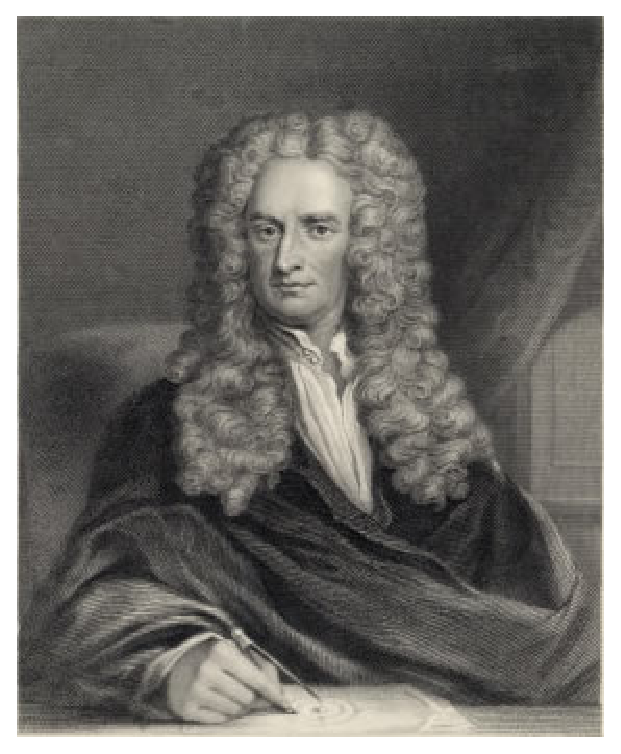
\includegraphics[width=3.5cm]{newton.eps}
      \captionsetup{singlelinecheck=off,justification=raggedright}%,margin={1mm,0mm}
\caption{Newton}
    \end{minipage}%
       \begin{minipage}[t]{.7\textwidth}
       \vspace{10pt}
Los principales descubrimientos matem�ticos de Newton en el campo del c�lculo infinitesimal datan de los llamados \emph{Anni Mirabiles} 1665 y 1666. La Universidad de Cambridge, en la que Newton se hab�a graduado como \emph{bachelor of arts} en 1664, estuvo cerrada por la peste esos dos a�os. Newton pas� ese tiempo en su casa de Woolsthorpe y, como �l mismo reconoci� cincuenta a�os despu�s, �se fue el per�odo m�s creativo de su vida.
\end{minipage}
\end{center}
\end{figure}\pagebreak

A principios de 1665 descubre el teorema del binomio y el c�lculo con las series infinitas. A finales de ese mismo a�o, el m�todo de fluxiones, es decir, el c�lculo de derivadas. En 1666 el m�todo inverso de fluxiones y la relaci�n entre cuadraturas y fluxiones. En esos dos a�os tambi�n inici� las teor�as de los colores y de la gravitaci�n universal. Newton ten�a 24 a�os, hab�a nacido el d�a de Navidad de 1642.

Newton desarroll� tres versiones de su c�lculo. En la obra \emph{De Analysi per aequationes numero terminorum infinitas}, que Newton entreg� a su maestro Barrow en 1669, y que puede considerarse el escrito fundacional del C�lculo, Newton usa conceptos infinitesimales de manera similar a como hac�a el propio Barrow.

Una segunda presentaci�n del C�lculo es la que realiza Newton en el libro \emph{Methodus fluxionum et serierum infinitorum}, \label{pag:fluxiones} escrito hacia 1671 y que se public� mucho despu�s en 1736. Newton considera cantidades variables que van fluyendo con el tiempo, a las que llama \emph{fluentes}. Despu�s se introducen las razones de cambio instant�neas de las fluentes, a las que llama \emph{fluxiones}, que son las derivadas respecto al tiempo de las fluentes. Newton representaba a las primeras por letras $x, y, z,\dots$ y a las segundas por letras punteadas $\dotup{x}, \dotup{y}, \dotup{z},\dots$. Los incrementos de las fluentes $x, y, z,\dots$, los representa por medio de las correspondientes fluxiones en la forma $\dotup{x}o,\dotup{y}o,\dotup{z}o,\dots$, y los llama \emph{momentos}, donde $o$ es entendido como un incremento infinitesimal de tiempo. Newton desarroll� una serie de algoritmos y redujo muchos problemas como determinaci�n de tangentes, m�ximos y m�nimos, �reas y superficies, curvaturas, longitudes de arcos, centros de gravedad etc., a dos problemas fundamentales que pueden formularse tanto en t�rminos mec�nicos como en t�rminos matem�ticos:
\begin{description}
  \item[Problema 1] Determinaci�n de la velocidad de movimiento en un momento de tiempo dado seg�n un camino dado. De otro modo: dada la relaci�n entre las cantidades fluentes, determinar la relaci�n de las fluxiones.
  \item[Problema 2] Dada la velocidad de movimiento determinar el camino recorrido en un tiempo dado. Matem�ticamente: determinar la relaci�n entre las fluentes dada la relaci�n entre las fluxiones.
\end{description}
Hay que notar que Newton no piensa en t�rminos de funciones con el significado actual de ese t�rmino, sino que imagina curvas o superficies descritas por las variables, o sea, considera relaciones entre las fluentes del tipo $f(x,y,z,\dots)=0$, donde $f$ para �l es una expresi�n anal�tica finita o infinita. Por tanto, el primer problema planteado puede verse como un problema de derivaci�n impl�cita: supuesta conocida la expresi�n anal�tica que satisfacen las fluentes $f(x,y,z,\dots)=0$, obtener la expresi�n anal�tica $F(x,y,z,\dotup{x},\dotup{y},\dotup{z},\dots)=0$ que satisfacen las fluxiones. Para este problema, Newton introdujo un algoritmo que sistematizaba los c�lculos necesarios. Por ejemplo, sea la curva de ecuaci�n
$$
x^3-ax^2+axy-y^3=0
$$
Sustituyendo $x$ e $y$ por $x+\dotup{x}o$ e $y+\dotup{y}o$ respectivamente, tenemos:
\begin{multline*}
(x^3+3\dotup{x}ox^2+3\dotup{x}^2o^2x+\dotup{x}^3o^3)-a(x^2+2\dotup{x}ox+\dotup{x}^2o^2)+
\\
+a(xy+\dotup{x}oy+\dotup{y}ox+\dotup{x}\ddotup{y}o^2)-(y^3+3\dotup{y}ox^2+3\dotup{y}^2o^2y+\dotup{y}^3o^3)=0
\end{multline*}
Teniendo en cuenta ahora que $x^3-ax^2+axy-y^3=0$, dividiendo por $o$ y despreciando los dem�s t�rminos que contengan a $o$, resulta
$$
3\dotup{x}x^2-2a\dotup{x}x+a\dotup{x}y+ax\dotup{y}-3\dotup{y}y^2=0
$$
Esta es la relaci�n que satisfacen las fluxiones. A partir de ella puede obtenerse la tangente a la curva $x^3-ax^2+axy-y^3=0$ en cualquier punto $(x,y)$ de la misma, que viene dada por:
$$
\frac{\dotup{y}}{\dotup{x}}=\frac{3x^2-2ax+ay}{3y^2-ax}
$$
Como ya hemos indicado, Newton aplica los resultados sobre fluentes y fluxiones a la resoluci�n de multitud de problemas. Por ejemplo, con respecto a los problemas de m�ximos y m�nimos, escribe:
\begin{quote}
\small{Cuando una cantidad es la m�s grande o la m�s peque�a, en ese momento su fluir ni crece ni decrece: si creciera, eso probar�a que era menor y que lo que sigue ser�a m�s grande que lo que ahora es, y rec�procamente pasar�a si decreciera. As�, calc�lese su fluxi�n como se ha explicado en el problema 1 e igu�lese a cero.}
\end{quote}
De nuevo, Newton usa el teorema fundamental del c�lculo para realizar cuadraturas. Escribe:
\begin{quote}
\small{Problema 9: Determinar el �rea de cualquier curva propuesta.

La resoluci�n del problema est� basada en el establecimiento de la relaci�n entre la cantidad fluente y su fluxi�n (problema 2).}
\end{quote}
Newton reduce la integraci�n al proceso inverso del c�lculo de fluxiones, esto es, al c�lculo de primitivas.

El problema 2, es mucho m�s dif�cil que el problema 1, pues se trata de resolver una ecuaci�n diferencial que puede ser muy general. Newton consider� varias posibilidades resolviendo algunos casos particulares. Para ello utiliz� t�cnicas de c�lculo de primitivas y de desarrollos en serie.

En \emph{De Quadratura Curvarum}, escrita en 1676 y publicada en 1704, Newton propone fundamentar su c�lculo de fluxiones en lo que llama \emph{razones primera y �ltima de incrementos evanescentes}. De esa forma se refiere Newton a los cocientes de los incrementos infinitesimales de las cantidades variables, y su objetivo es determinarlos en el momento en que dichas cantidades nacen desde cero (``raz�n primera'') o se anulan (``raz�n �ltima''). Un ejemplo ayudar� a entender el significado de estas ideas. En la introducci�n de la citada obra, Newton calcula la fluxi�n de $x^n$. Para ello, considera un incremento $o$ de forma que $x$ pasa a $x+o$. Entonces $x^n$ se convierte en
$$
(x+o)^n=x^n+nox^{n-1}+\frac{n(n-1)}{2}o^2x^{n-2}+\cdots
$$
Los incrementos de $x$ y $x^n$, a saber,
$$o\quad \textrm{y}\quad  nox^{n-1}+\frac{n(n-1)}{2}o^2x^{n-2}+\cdots$$ est�n entre s� en la misma raz�n que
$$1\quad \textrm{a}\quad nx^{n-1}+\frac{n(n-1)}{2}ox^{n-2}+\cdots$$
Dice Newton ``dejemos ahora que los incrementos se anulen y su �ltima proporci�n ser� $1$ a $nx^{n-1}$: por tanto, la fluxi�n de la cantidad $x$ es a la fluxi�n de la cantidad $x^n$ como $1:nx^{n-1}$''.

Hay distintas interpretaciones de las razones que llevaron a Newton a exponer su c�lculo de una u otra forma. La m�s extendida es que su intenci�n era  conseguir una fundamentaci�n rigurosa del mismo. La primera exposici�n, basada en el concepto de cantidad infinitesimal, entendida como una cantidad menor que cualquier cantidad positiva pero no nula, presentaba problemas de coherencia l�gica de los que Newton era muy consciente. En sus propias palabras, su c�lculo estaba \emph{``concisamente explicado m�s que exactamente demostrado''}.

En \emph{Methodus Fluxionum et Serierum Infinitarum} (1671), el concepto b�sico es el de cantidad en movimiento o que fluye continuamente en el tiempo. Las magnitudes est�n generadas por el movimiento continuo y no por agregaci�n de cantidades infinitesimales; la idea b�sica es la de continuidad tal como se observa en los procesos de la Naturaleza. Quiz�s Newton pretend�a de esta forma evitar el uso de ``infinitesimales est�ticos o geom�tricos'', pero lo que realmente hizo fue sustituirlos por los infinitesimales de tiempo usados para definir los momentos de las fluentes. Conviene advertir que lo que Newton considera es la abstracci�n matem�tica an�loga al tiempo, es decir, una magnitud independiente imaginaria abstracta que fluye uniformemente y con la que se relacionan todas las fluentes. Puede verse aqu� un intento de Newton por evitar los problemas matem�ticos del continuo (infinitesimales, indivisibles) y trasladarlos al mundo f�sico, a la continuidad de los procesos naturales y al movimiento. Por otra parte, Newton aceptaba como algo dado la idea intuitiva de velocidad instant�nea de las fluentes, no le pareci� preciso definirla.

En \emph{Quadrature of Curves} (1676), Newton expresa su prop�sito de abandonar por completo el uso de  cantidades infinitesimales. Manifiesta en este sentido que \emph{``errores quam minimi in rebus mathematicis non sunt contemnendi''}, esto es, que en matem�ticas ni siquiera los errores m�s peque�os pueden ser admitidos. Y eso es justamente lo que se hac�a cuando se despreciaban en los c�lculos cantidades infinitesimales. Seguidamente, enuncia su teor�a de las \emph{``razones primera y �ltima de cantidades evanescentes''}.
Estas ideas se�alan claramente al concepto matem�tico de l�mite. Lo que expresa, a su manera, Newton es, en t�rminos actuales, el l�mite de un cociente de funciones que se anulan. Pero estamos en el siglo XVII y se necesitar�n casi 200 a�os para precisar matem�ticamente el concepto de l�mite. Debemos notar que Newton usa dicho concepto a partir de la intuici�n mec�nica del movimiento.
\begin{quote}
\small{Por velocidad �ltima se entiende aquella con la que el cuerpo se mueve, no antes de alcanzar el punto final y cesa, por consiguiente, el movimiento, ni tampoco despu�s de haberlo alcanzado, sino aquella con la que se mueve cuando lo alcanza, esto es, aquella velocidad con la que el cuerpo alcanza el punto final y aquella con la que cesa el movimiento. De igual manera, ha de entenderse por raz�n �ltima de cantidades evanescentes, la raz�n de cantidades, no antes de que desaparezcan, ni despu�s de desaparecidas, sino aquella con la que desaparecen.}
\end{quote}
Newton ten�a su particular idea de ``l�mite''.
\begin{quote}
\small{Las razones �ltimas con las que tales cantidades desaparecen en realidad no son razones de cantidades �ltimas, sino l�mites a los que tiende a acercarse siempre las razones de cantidades continuamente decrecientes, l�mites a los que pueden acercarse m�s que una diferencia dada, pero nunca traspasarlo, ni tampoco alcanzarlo antes de que las cantidades disminuyan in infinitum.}
\end{quote}
La teor�a de las razones �ltimas puede verse como una teor�a cinem�tica de l�mites. Con esta teor�a, Newton pretend�a recuperar el rigor de la geometr�a de la Antig�edad.
\begin{quote}
\small{[\dots] investigar las razones primera y �ltima de cantidades finitas, nacientes o evanescentes, est� en armon�a con la geometr�a de los antiguos; y me he esforzado en probar que, en el m�todo de fluxiones, no es necesario introducir en la geometr�a cantidades infinitamente peque�as.}
\end{quote}

Otros autores opinan que estos tres m�todos empleados por Newton responden, m�s que a fundamentar con rigor su c�lculo, a distintos prop�sitos. As�, la teor�a de fluxiones proporciona m�todos heur�sticos de descubrimiento y algoritmos �tiles para el calculo; la teor�a de ``razones primera y �ltima'' servir�a al prop�sito de proporcionar demostraciones convincentes y el uso de los infinit�simos servir�a para proporcionar atajos a las pruebas m�s rigurosas. Newton us� simult�neamente estas tres aproximaciones en la resoluci�n de una gran variedad de problemas.

Newton realiz� tambi�n contribuciones importantes en la teor�a de ecuaciones, donde podemos destacar las ``identidades de Newton'' para la suma de las potencias de las ra�ces de una ecuaci�n polin�mica, y a la teor�a de curvas, siendo notable su clasificaci�n de las curvas de tercer grado.
\begin{quote}
\emph{Considerando la matem�tica desde el comienzo del mundo hasta la �poca de Newton, lo que �l ha hecho es, con mucho, la mitad mejor.}\hfill Leibniz
\end{quote}

Las tres obras consideradas, escritas entre 1666 y 1676, se publicaron ya en el siglo XVIII, por eso la primera noticia impresa de la teor�a de fluxiones apareci�, de forma bastante circunstancial, en la obra magna de Newton \emph{Philosophiae Naturalis Principia Mathematica}, cuya primera edici�n se hizo en 1687. Los \emph{Principia} consta de tres libros escritos en el estilo tradicional a la manera de los \emph{Elementos} de Euclides, y su lenguaje es principalmente el de la geometr�a sint�tica.

Los \emph{Principia} est�n considerados como la obra cient�fica m�s importante de todos los tiempos y una haza�a intelectual incomparable por sus logros y sus consecuencias. En dicha obra Newton estable los fundamentos de la mec�nica y enuncia las tres c�lebres leyes del movimiento, as� como la ley de la gravitaci�n universal. En los dos primeros libros, se estudia el movimiento de los cuerpos en el vac�o y en un medio resistente. Newton deduce matem�ticamente las tres leyes que Kepler hab�a obtenido emp�ricamente. En el libro III, titulado \emph{Sobre el Sistema del Mundo}, Newton desarrolla la mec�nica celeste. Hace un detallado estudio de los movimientos de la Luna, explicando las causas de las mareas. Calcula la masa del Sol con respecto a la de la Tierra, estudia la precesi�n de los equinoccios, predice el achatamiento de la Tierra por los polos \dots .

En los \emph{Principia} el mundo aparece como un sistema ordenado y armonioso en el que todo, los cielos, la tierra y el mar, obedecen unas pocas leyes matem�ticas fundamentales. A partir de Newton quedar� claro que no hay diferencias entre un mundo sublunar y otro supralunar, ni entre la Tierra y el Cielo; las leyes de la Naturaleza no hacen estas distinciones y en todas partes del Universo los procesos obedecen a las mismas leyes naturales inexorables.

El Universo newtoniano es un Cosmos di�fano y sereno ofrecido a la exploraci�n racional del hombre. La gran obra de Newton proporcionar� a la Ilustraci�n, en el siglo XVIII, la base cient�fica necesaria para acabar con una concepci�n conservadora y absolutista del poder pol�tico apoyada en dogm�ticas concepciones religiosas.

El prestigio y admiraci�n que goz� Newton en vida queda reflejado en las palabras de Alexander Pope:\vspace*{-2mm}
\begin{quote}
\emph{Nature, and Nature's Laws lay hid in Night:}\newline
\emph{God said, \emph{Let Newton be} -- and All was light.}
\end{quote}\vspace*{-2mm}
Y �qu� pensaba el propio Newton de s� mismo? Escuchemos sus palabras, ya casi al final de su vida.\vspace*{-2mm}
\begin{quote}
\small{No s� c�mo puedo ser visto por el mundo, pero a m� me parece haber sido solamente como un ni�o que juega al borde del mar, y que se divierte al encontrar de vez en cuando una piedra m�s pulida o una concha m�s bonita de lo normal, mientras que el gran oc�ano de la verdad yace ante m� completamente desconocido.}
\end{quote}\vspace*{-2mm}
Newton muri� en la noche del 20 de marzo de 1727, y fue enterrado con grandes honores en la abad�a de Westminster entre los grandes hombres de Inglaterra.

\subsection{Leibniz y el c�lculo de diferencias}
\vspace*{-2mm}
\begin{figure}[ht]
\begin{center}
\begin{minipage}[t]{.3\textwidth}
\vspace{10pt}
\flushleft
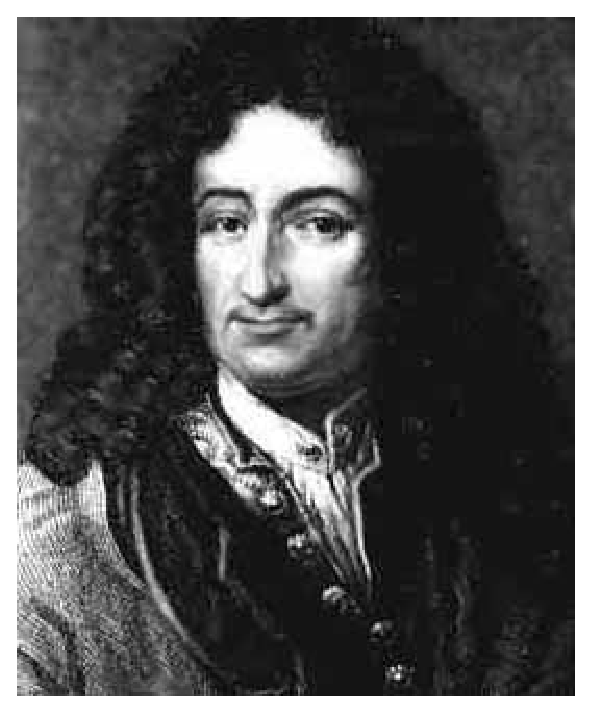
\includegraphics[width=3.5cm]{leibniz.eps}
      \captionsetup{singlelinecheck=off,justification=raggedright}%,margin={1mm,0mm}
\caption{Leibniz}
    \end{minipage}%
       \begin{minipage}[t]{.7\textwidth}
       \vspace{0pt}
Gottfried Wilhelm Leibniz (1646 - 1716)\label{pag:leibniz} naci� en Leipzig (Alemania) en el seno de una piadosa familia luterana. A los quince a�os entr� en la Universidad de su ciudad natal donde estudi� una gran variedad de materias incluyendo derecho, teolog�a, filosof�a y matem�ticas. Se doctor� a la edad de 21 a�os en la Universidad de Altdorf, en Nuremberg, donde le fue ofrecido un puesto de profesor que �l rechaz�.

A lo largo de su vida, Leibniz realiz� m�ltiples actividades. Como abogado y diplom�tico trabaj� para el Pr�ncipe elector arzobispo de Maguncia y, desde 1676 hasta su muerte, para los Duques de Brunswick-Luneburgo (conocidos como pr�ncipes electores de Hanover desde 1692), lo que le llev� a viajar por gran parte de Europa. Invent� una m�quina de calcular, la primera m�quina de este\linebreak
\end{minipage}
\end{center}
\end{figure}\vspace{-12mm}

\noindent tipo capaz de realizar las operaciones de multiplicaci�n, divisi�n y extracci�n de ra�ces cuadradas. Como ingeniero trabaj� en prensas hidr�ulicas, molinos de viento y desarroll� proyectos para drenar el agua de las minas de plata de las monta�as de Harz en la Baja Sajonia. Como historiador escribi� la historia de la casa de Brunswick, realizando muchas investigaciones geneal�gicas. Trabaj� tambi�n como bibliotecario en la ciudad de Hanover.

Leibniz fue un pensador profundo. Como fil�sofo se propuso la creaci�n de un �lgebra del pensamiento humano, algo as� como un lenguaje simb�lico universal para escribir los razonamientos con s�mbolos y f�rmulas, cuyas reglas de combinaci�n permitieran reducir todo discurso racional a c�lculos rutinarios. Esto explica el gran inter�s de Leibniz en desarrollar una notaci�n matem�tica apropiada para su c�lculo; de hecho, su notaci�n, muy superior a la de Newton, es la que usamos actualmente. Leibniz fund� la Academia de Ciencias de Berl�n en 1700 y fue su primer presidente; tambi�n fue uno de los fundadores de la primera revista cient�fica alemana, el \emph{Acta Eruditorum}.

Aunque Leibniz public� poco, mantuvo correspondencia con m�s de 600 eruditos y se han conservado sus manuscritos que est�n en el archivo que lleva su nombre en la ciudad de Hannover. Las contribuciones de Leibniz al �lgebra (determinantes, resoluci�n de ecuaciones), la historia natural, la geolog�a y la ling��stica son tambi�n importantes.

En 1672, estando en Par�s en misi�n diplom�tica, Leibniz se dedic� intensamente al estudio de la matem�tica superior teniendo como gu�a al matem�tico y f�sico Christian Huygens (1629 - 1695). En los a�os 1673 y 1676 realiz�, tambi�n en misi�n diplom�tica, dos viajes a Londres donde tuvo acceso al manuscrito de Newton \emph{De Analysi}, circunstancia que se us� para acusar, hoy sabemos que sin motivo alguno, a Leibniz de plagio cuando se produjo la agria controversia sobre la prioridad en el descubrimiento del C�lculo. Los progresos matem�ticos realizados por Leibniz en estos cuatro a�os fueron extraordinarios.

En las matem�ticas de Leibniz son importantes los estudios sobre sucesiones num�ricas y sus sucesiones de diferencias consecutivas asociadas. Dada una sucesi�n de n�meros:
$$
a_1, a_2, a_3, a_4,\dots, a_{n-1}, a_n,\dots
$$
Podemos formar la sucesi�n de sus diferencias primeras:
$$
b_1=a_1, b_2=a_2-a_1, b_3=a_3-a_2, b_4=a_4-a_3,\dots, b_n=a_n-a_{n-1},\dots
$$
Leibniz se hab�a dado cuenta de la relaci�n:
$$
b_1+b_2+b_3+\cdots+b_n=a_n
$$
lo que indica que las sucesiones de diferencias pueden sumarse f�cilmente, y que el proceso de formar la sucesi�n de diferencias y despu�s sumarla recupera la sucesi�n inicial, es decir, que se trata de operaciones inversas una de la otra. Esta sencilla idea, cuando se lleva al campo de la geometr�a, conduce al concepto central del c�lculo de Leibniz que es el de ``diferencial'', el cual tuvo para �l diferentes significados en distintas �pocas.

Leibniz consideraba una curva como un pol�gono de infinitos lados de longitud infinitesimal. Con una tal curva se asocia una sucesi�n de abscisas
$
x_1, x_2, x_3, x_4,\dots
$
y una sucesi�n de ordenadas
$
y_1, y_2, y_3, y_4,\dots
$
donde los puntos $(x_i,y_i)$ est�n todos ellos en la curva y son algo as� como los ``v�rtices'' de la poligonal de infinitos lados que forma la curva. La diferencia entre dos valores sucesivos de $x$ es llamada la \emph{diferencial} de $x$ y se representa por $\df{x}$, significado an�logo tiene $\df{y}$. El diferencial $\df{x}$ es una cantidad fija, no nula, infinitamente peque�a en comparaci�n con $x$, de hecho es una cantidad infinitesimal. Los lados del pol�gono que constituye la curva son representados por $\df{s}$. Resulta as� el \emph{tri�ngulo caracter�stico} de Leibniz que es el mismo que ya hab�a sido considerado por Barrow.

Curiosamente, los t�rminos ``abscisa'', ``ordenada'' y ``coordenadas'', tan propios de la geometr�a anal�tica, no fueron usados nunca por Descartes sino que son debidos a Leibniz; y mientras que nosotros hablamos de ``diferenciales'', Leibniz siempre hablaba de ``diferencias''.

\begin{figure}[ht]
\centering
\begin{pspicture}(-2.5,0)(6,4.5)
\psset{yunit=1.5cm,xunit=.7cm, arrowscale=1.4,labelsep=3pt}
\psplot[algebraic,plotpoints=500]{.2}{6}{sqrt(x)}
\psline[linewidth=.6pt]{->}(-1.2,0)(6,0)
\psline[linewidth=.6pt]{->}(-1,-.2)(-1,2.5)
\psline[linewidth=.4pt](2,0)(2,1.414)(3,1.414)
%\psline[linewidth=.4pt](-2,0)(5,2.475)
\psline[linewidth=.4pt](3,0)(3,1.73)
\uput[u](.5,0){\scalefont{.7}$x$}
\uput[l](2,.7){\scalefont{.7}$y$}
\uput[u](2.4,1.55){\scalefont{.7}$\df{s}$}
\uput[d](2.5,1.46){\scalefont{.7}$\df{x}$}
\uput[r](2.85,1.6){\scalefont{.7}$\df{y}$}
\end{pspicture}
\caption{Tri�ngulo caracter�stico}\label{fig:tricar}
\end{figure}

El tri�ngulo caracter�stico tiene lados infinitesimales $\df{x}$, $\df{y}$, $\df{s}$ y se verifica la relaci�n $(\df{s})^2=(\df{x})^2+(\df{y})^2$. El lado $\df{s}$ sobre la curva o pol�gono se hace coincidir con la tangente a la curva en el punto $(x,y)$. La pendiente de dicha tangente viene dada por $\frac{\df{y}}{\df{x}}$, que es un cociente de diferenciales al que Leibniz llam� \emph{cociente diferencial}. Leibniz nunca consider� la derivada como un l�mite.

Leibniz investig� durante alg�n tiempo hasta encontrar las reglas correctas para diferenciar productos y cocientes. Dichas reglas se expresan f�cilmente con su notaci�n diferencial:
$$
\df{(x y)}=y\df{x}+x\df{y},\qquad\df{\left(\dfrac{x}{y}\right)}=\dfrac{y\df{x}-x\df{y}}{y^2}
$$
La manera en que Leibniz lleg� a estas f�rmulas pudo ser como sigue. Consideremos
$$
z_n=\left(\sum_{j=1}^n x_j\right)\left(\sum_{j=1}^n y_j\right)
$$
Entonces
\begin{equation}\label{reglaproducto}
    z_{n+1}-z_n=x_{n+1}\sum_{j=1}^{n+1}y_j+y_{n+1}\sum_{j=1}^n x_j
\end{equation}
Si interpretamos, al estilo de Leibniz, que $x_j$ e $y_j$ son diferencias de valores consecutivos de las cantidades $x$ e $y$ respectivamente, entonces los valores de dichas cantidades vendr�n dados por las sumas respectivas $x=\sum_{j=1}^n x_j$ e $y=\sum_{j=1}^{n+1}y_j$, mientras que $\df{x}=x_{n+1}$ y $\df{y}=y_{n+1}$ por ser diferencias de valores consecutivos. De la misma forma, $z_{n+1}-z_n$ ser�a la diferencial de $z=xy$. Por tanto, la igualdad \ref{reglaproducto}\ es interpretada por Leibniz en la forma $\df{(x y)}=x\df{y}+y\df{x}$, lo que lleva a la regla para la diferencial de un producto.

A partir de la regla para la diferencial de un producto, Leibniz obtuvo la regla correspondiente para la diferencial de un cociente $z=\frac{x}{y}$. Poniendo $x=zy$ se tiene que $\df{x}=y\df{z}+z\df{y}$, de donde despejando $\df{z}$, resulta:
$$
\df{z}=\frac{\df{x}-z\df{y}}{y}=\frac{\df{x}-\frac{x}{y}\df{y}}{y}=\frac{y\df{x}-x\df{y}}{y^2}
$$
Adem�s, dicha notaci�n tiene una gran potencialidad heur�stica, como ya hemos visto al estudiar la derivada de una funci�n compuesta.

Consideremos ahora una curva como la de la figura \ref{fig:Lz-integ} con una sucesi�n de ordenadas trazadas a intervalos de longitud unidad.
\begin{figure}[ht]
\centering
\begin{pspicture}(0,0)(8,4.5)
\psset{yunit=1.5cm,xunit=1cm, arrowscale=1.4, labelsep=2pt}
\psaxes[linewidth=.5pt, labels=none, ticks=none]{->}(0,0)(8,2.5)
\psplot[algebraic,plotpoints=500]{0}{6.5}{sqrt(x)}
\psline[linewidth=.5pt](.5,0)(!.5 .5 sqrt)
\psline[linewidth=.5pt](1,0)(1,1)
\psline[linewidth=.5pt](1.5,0)(!1.5 1.5 sqrt)
\psline[linewidth=.5pt](2,0)(!2 2 sqrt)
\psline[linewidth=.5pt](2.5,0)(!2.5 2.5 sqrt)
\psline[linewidth=.5pt](3,0)(!3 3 sqrt)
\psline[linewidth=.5pt](3.5,0)(!3.5 3.5 sqrt)
\psline[linewidth=.5pt](4,0)(!4 4 sqrt)
\psline[linewidth=.5pt](4.5,0)(!4.5 4.5 sqrt)
\psline[linewidth=.5pt](5,0)(!5 5 sqrt)
\psline[linewidth=.5pt](5.5,0)(!5.5 5.5 sqrt)
\psline[linewidth=.5pt](6,0)(!6 6 sqrt)
\psline[linewidth=.5pt](6.5,0)(!6.5 6.5 sqrt)
\uput[r](!.5 .5 sqrt 2 div){\scalefont{.6}$y_1$}
\uput[r](1,.5){\scalefont{.6}$y_2$}
\uput[r](!1.5 1.5 sqrt 2 div){\scalefont{.6}$y_3$}
\uput[r](!2 2 sqrt 2 div){\scalefont{.6}$y_4$}
\uput[r](!2.5 2.5 sqrt 2 div){\scalefont{.6}$y_5$}
\uput[r](!3 3 sqrt 2 div){\scalefont{.6}$y_6$}
\uput[r](!3.5 3.5 sqrt 2 div){\scalefont{.6}$y_7$}
\uput[r](!4 4 sqrt 2 div){\scalefont{.6}$y_8$}
\uput[r](!4.5 4.5 sqrt 2 div){\scalefont{.6}$y_9$}
\uput[r](!5 5 sqrt 2 div){\scalefont{.6}$y_{10}$}
\uput[r](!5.5 5.5 sqrt 2 div){\scalefont{.6}$y_{11}$}
\uput[r](!6 6 sqrt 2 div){\scalefont{.6}$y_{12}$}
\uput[r](!6.5 6.5 sqrt 2 div){\scalefont{.6}$y_{13}$}
\psset{labelsep=7pt}
\multido{\n=0.0+0.5}{13}{%
\uput[dr](\n,0.07){\scalefont{.6}$1$}
}
\end{pspicture}
\caption{Aproximaci�n de una cuadratura}\label{fig:Lz-integ}
\end{figure}
\label{pag:leibniz}La suma de las ordenadas es una aproximaci�n de la cuadratura de la curva (del �rea bajo la curva), y la diferencia entre dos ordenadas sucesivas es aproximadamente igual a la pendiente de la correspondiente tangente. Cuanto m�s peque�a se elija la unidad 1, tanto mejor ser�n estas aproximaciones. Leibniz razonaba que si la unidad pudiera ser tomada \emph{infinitamente peque�a}, estas aproximaciones se har�an exactas, esto es, la cuadratura ser�a igual a la suma de las ordenadas, y la pendiente de la tangente ser�a igual a la diferencia de dos ordenadas sucesivas. Como las operaciones de tomar diferencias y sumar son rec�procas entre s�, dedujo Leibniz que el c�lculo de cuadraturas y de tangentes tambi�n eran operaciones inversas una de otra.

Las investigaciones de Leibniz sobre la integraci�n y el origen de sus notaciones para la integral y los diferenciales, pueden seguirse con todo detalle en una serie de manuscritos del 25 de octubre al 11 de noviembre de 1675. Nos ocuparemos de ello en el cap�tulo dedicado a la integraci�n.
En 1676 Leibniz ya hab�a obtenido pr�cticamente todos los resultados descubiertos por Newton un poco antes.

La primera publicaci�n sobre c�lculo diferencial fue el art�culo de Leibniz \emph{Nova methodus pro maximis et minimis, itemque tangentibus, quae nec fractals nec irrationales quantitates moratur, et singulare pro illis calculi genus}, que fue publicado en \emph{Acta Eruditorum} hace ya m�s de tres siglos, en 1684. En este trabajo, Leibniz defin�a el diferencial $\df{y}$ de forma que evitaba el uso de las sospechosas cantidades infinitesimales. Poco despu�s, en 1686, Leibniz public� un trabajo con sus estudios sobre la integraci�n.

%Mientras que Barrow utiliz� el tri�ngulo caracter�stico de una forma exclusivamente geom�trica, Leibniz fue capaz de expresar anal�ticamente, mediante f�rmulas sencillas, las transformaciones integrales que se obtienen a partir de dicho tri�ngulo.

%The name �coordinate� does not appear in the work of Descartes. This term is due to Leibniz, and so are �abscissa� and �ordinate� (1692).

Reconocido hoy d�a como un genio universal, Leibniz vivi� sus �ltimos a�os en Hannover en un aislamiento cada vez mayor y muri� el 14 de noviembre de 1716. A su entierro solamente asisti� su secretario.

\subsection{Desarrollo del c�lculo diferencial}
Aunque las publicaciones de Leibniz eran breves y dif�ciles de leer, su c�lculo, m�s sencillo de entender que el de Newton y provisto de una excelente notaci�n, triunf� pronto en el continente europeo logrando grandes �xitos, mientras que en Inglaterra la fidelidad a la teor�a de fluxiones y a la notaci�n newtoniana condujo a un cierto aislamiento, agravado por sentimientos nacionales y la disputa sobre la prioridad, y no consigui� �xitos comparables a los del continente.

Los hermanos Jakob y Johann Bernouilli, matem�ticos y profesores de la universidad de Basilea, estudiaron los trabajos de Leibniz con quien iniciaron una productiva correspondencia. A partir de 1690 publicaron una serie de trabajos en el \emph{Acta Eruditorum} y en otras revistas, poniendo de manifiesto que el c�lculo de Leibniz era una herramienta poderosa con la que hab�a que contar. Para divulgar dicha herramienta era preciso un buen libro de texto que explicara con detalle los pormenores del nuevo c�lculo. Dicho libro apareci� bien pronto, en 1696, y su autor fue el matem�tico y noble franc�s Guillaume Fran\c{c}ois, marqu�s de L'H�pital. El t�tulo del libro, del que ya hemos dado noticia en anteriores cap�tulos, era \emph{Analyse des infiniment petits pour l'intelligence des lignes courbes}. Hoy sabemos que los resultados originales que aparecen en dicho libro son debidos no a L'H�pital sino a su profesor Johann Bernouilli.

En su libro, L'H�pital desarrollaba el c�lculo diferencial tal como hab�a sido concebido por Leibniz, es decir, usando cantidades infinitesimales para las que se establec�an ciertas reglas de c�lculo. La definici�n de diferencial es como sigue: \emph{``La parte infinitamente peque�a en que una cantidad variable es aumentada o disminuida de manera continua, se llama la diferencial de esta cantidad''}. Para trabajar con infinit�simos se establece la siguiente regla: \emph{``Dos cantidades cuya diferencia es otra cantidad infinitamente peque�a pueden intercambiarse una por la otra''}.

Los escritos de los Bernouilli, Leibniz y L'H�pital popularizaron el c�lculo leibniziano y ya en la primera d�cada del siglo XVIII otros matem�ticos se interesaron por �l. La potencialidad del concepto de derivada se puso de manifiesto en las aplicaciones del c�lculo a la f�sica newtoniana.

Para no hacer excesivamente larga esta exposici�n, voy a resumir muy esquem�ticamente los puntos clave en el desarrollo del c�lculo diferencial.

\begin{list}{$\bullet$}{\addtolength{\itemsep}{-6pt}}
\item El descubrimiento en 1715 por Brook Taylor de las llamadas series de Taylor, que se convirtieron en una herramienta b�sica para el desarrollo del c�lculo y la resoluci�n de ecuaciones diferenciales.
\item El extraordinario trabajo, tanto por su asombrosa amplitud como por sus notables descubrimientos, de Leonhard Euler (1707 - 1783) que, sin duda, es la figura principal de las matem�ticas en el siglo XVIII. En sus tres grandes tratados, escritos en lat�n, \emph{Introductio in analysin infinitorum} (1748), \emph{Institutiones calculi differentiales} (1755) e \emph{Institutiones calculi integralis} (1768), Euler dio al c�lculo la forma que conserv� hasta el primer tercio del siglo XIX. El c�lculo, que inicialmente era un c�lculo de variables o, m�s exactamente, de cantidades geom�tricas variables, y de ecuaciones, se fue transformando, por influencia de Euler, en un c�lculo de funciones.
\item  La propuesta de Joseph Louis Lagrange (1736 - 1813) de fundamentar el c�lculo sobre un �lgebra formal de series de potencias. Si bien la idea de Lagrange de evitar el uso de l�mites no era acertada, su propuesta, concretada en su obra \emph{Th�orie des fonctions analytiques} (1797), tuvo el efecto de liberar el concepto de derivada de sus significaciones m�s tradicionales. De hecho, la terminolog�a ``funci�n derivada'', as� como la notaci�n $f\tl(x)$ para representar la derivada de una funci�n $f$, fueron introducidas por Lagrange en dicho texto. A partir de este momento la derivada deja de ser algo de naturaleza imprecisa (fluxi�n o cociente diferencial) y empieza a ser considerada simplemente como una funci�n.
\item Los problemas planteados por las series de Fourier. Dichas series hacen sus primeras apariciones a mitad del siglo XVIII en relaci�n con el problema de la cuerda vibrante, y nacen oficialmente en el trabajo de Joseph Fourier (1768 - 1830) \emph{Th�orie analytique de la chaleur} (1822). Tales series plantean problemas relacionados con las ideas centrales del an�lisis: el concepto de funci�n, el significado de la integral y los procesos de convergencia.
\item El proceso de ``algebraizaci�n del an�lisis'' que tiene lugar en los dos �ltimos tercios del siglo XIX y que culmina con la fundamentaci�n del an�lisis sobre el concepto de l�mite (Bolzano, Cauchy, Weierstrass) y la teor�a de los n�meros reales (Dedekind, Cantor). Lo esencial de este proceso ya ha sido considerado en el cap�tulo anterior.
\end{list}

Si el tema te interesa, puedes encontrar mucha m�s informaci�n en las referencias citadas al principio.

\chapter{Sucesiones}

\section{Introducci�n}

Las sucesiones aparecen de manera natural en muchos c�lculos que
responden a un esquema iterativo. Por ejemplo, al dividir $2$
entre $3$ obtenemos ${\dis
\,\frac{2}{3}=\frac{6}{10}+\frac{2}{3}\frac{1}{10}\,}$, igualdad que
podemos usar ahora para obtener $$
\frac{2}{3}=\frac{6}{10}+\left(\frac{6}{10}
+\frac{2}{3}\frac{1}{10}\right)\frac{1}{10}
=\frac{6}{10}+\frac{6}{10^{2}}+\frac{2}{3}\frac{1}{10^{2}}, $$ y
de nuevo $$
\frac{2}{3}=\frac{6}{10}+\frac{6}{10^{2}}+\left(\frac{6}{10}
+\frac{2}{3}\frac{1}{10}\right)\frac{1}{10^{2}}=
\frac{6}{10}+\frac{6}{10^{2}}+\frac{6}{10^{3}}
+\frac{2}{3}\frac{1}{10^{3}}. $$ Y as� podemos continuar
tantas veces como queramos, obteniendo para cada $n\en\N$ la
igualdad: $$
\frac{2}{3}=\sumaf{k=1}{n}\frac{6}{10^{k}}\,+\,\frac{2}{3}\frac{1}{10^{n}}.
$$ Escribiendo ${\dis \,x_{n}=\sumaf{k=1}{n}\frac{6}{10^{k}}\,}$ tenemos que ${\dis
\,0<\frac{2}{3}-x_{n}=\frac{2}{3}\frac{1}{10^{n}}}$. Observa que,
aunque los n�meros $x_{n}$ son {\em todos ellos distintos\/} de
$\,2/3$, dada una cota de error arbitrariamente peque�a, \epos, y
tomando $n_{0}\en\N$ de manera que \rule{0cm}{6mm} ${\dis \
\frac{2}{3}\frac{1}{10^{n_{0}}}<\varepsilon}\,$, deducimos que
{\em para todo\/} n\'umero natural $n\!\geqslant\!n_{0}$ se verifica
que \rule{0cm}{5mm} ${\dis \,|x_{n}-2/3|<\varepsilon}\,$, lo que se
expresa escribiendo ${\dis 2/3=\Lim{\sucn{x}}{n}{\infty}}$.

El ejemplo anterior est� relacionado con la expresi\'on decimal de
$2/3$ que, como todos sabemos, es un decimal peri\'odico con
per�odo igual a $6$, lo que suele escribirse
$\,2/3=0,\widehat{6}\,$ igualdad en la que, seg\'un se dice a
veces, el s�mbolo $\,0,\widehat{6}\,$ debe interpretarse como
que el $\,6\,$ \emph{se repite infinitas veces}. �Qu\'e quiere
decir esto? Lo que est� claro es que, por mucho tiempo y
paciencia que tengamos, nunca podremos escribir {\em infinitos\/}
$\,6\,$ uno detr\'as de otro... bueno, podr�amos escribir
algo como $$ \frac{2}{3}=0,\widehat{6}=0,6666666...({\rm
\,infinitos\,}6) $$ lo que tampoco sirve de mucho pues seguimos
sin saber c\'omo se interpreta esta igualdad. Pues bien, para dar
un significado matem\'atico a lo que se quiere expresar con esa
igualdad hay que recurrir al concepto de l�mite de una
sucesi\'on tal como hemos hecho antes.

Veamos otro ejemplo en esta misma l�nea. Vamos a intentar
calcular aproximaciones racionales de $\sqrt{10}$. Si partimos
inicialmente de un n\'umero $x>\sqrt{10}$, tendremos que ${\dis
\,\frac{10}{x}<\sqrt{10}<x}$. Pongamos ${\dis
\,y=\frac{1}{2}\left(x+\frac{10}{x}\right)}$. Entonces, en virtud de
la desigualdad de las medias, $\sqrt{10}<y$, y como tambi�n
$\,y<x\,$, deducimos que $\,y\,$ est� m\'as cerca de $\sqrt{10}$
que $x$. Podemos ahora repetir este proceso sustituyendo $\,x\,$ por
$\,y\,$ obteniendo una nueva aproximaci\'on mejor de $\sqrt{10}$.
N\'otese que si $x$ es racional tambi\'en lo ser� $y$. Esto
sugiere que, partiendo de un valor inicial, por ejemplo
$x_{1}\!=4$, calculemos ${\dis
\,x_{2}=\frac{1}{2}\left(x_{1}+\frac{10}{x_{1}}\right)}$, y
despu\'es ${\dis
\,x_{3}=\frac{1}{2}\left(x_{2}+\frac{10}{x_{2}}\right)}$, y as�
podemos continuar tantas veces como queramos, obteniendo para cada
$n\in\N$ un n\'umero $x_{n}$ tal que $$
x_{n+1}\!=\frac{1}{2}\left(x_{n}+\frac{10}{x_{n}}\right) $$ con
$x_{1}\!=4$. Con una calculadora manual obtenemos enseguida los
valores \makebox{$\,x_{2}\!=\!3,25$;}\linebreak \makebox{$\,
x_{3}\!=\!3,1634615\,;\ x_{4}\!=\!3,1622779\,$} con seis cifras
decimales exactas:
$$ 0<x_{4}-\sqrt{10}=\frac{x_{4}^{2}-10}{x_{4}+\sqrt{10}}<
\frac{x_{4}^{2}-10}{6}<\frac{0,000005}{6}<\frac{1}{10^{6}} $$ es
decir, $x_{4}$ coincide con $\sqrt{10}$ hasta la sexta cifra
decimal. De hecho, como $\makebox{$x_{n}\!>\!\sqrt{10}$}$ tenemos
que: $$
0<x_{n+1}-\sqrt{10}=\frac{1}{2}\left(x_{n}+\frac{10}{x_{n}}\right)-\sqrt{10}
<\frac{1}{2}x_{n}+\frac{1}{2}\sqrt{10}-\sqrt{10}=\frac{1}{2}(x_{n}-\sqrt{10})
$$ de donde se sigue que ${\dis
\,0<x_{n+1}-\sqrt{10}<\frac{1}{2^{n}}(x_{1}-\sqrt{10})<\frac{1}{2^{n}}}$,
por tanto, dado cualquier \epos, y tomando $n_{0}\in\N$ tal que
$\,2^{-n_{0}}<\varepsilon$, deducimos que {\em para todo} n\'umero
natural $\,n\geqslant n_{0}$ se verifica que
$\,|x_{n}-\sqrt{10}\,|<\varepsilon$, lo que simb�licamente se
expresa escribiendo \makebox{${\dis
\,\sqrt{10}=\Lim{\sucn{x}}{n}{\infty}}$}.

En los ejemplos anteriores hemos dado por supuesto que ya tienes
cierta familiaridad con los conceptos de ``sucesi\'on'' y de
``l�mite de una sucesi\'on'' de los cuales vamos a ocuparnos
a continuaci\'on con detalle.



\section{Sucesiones de n�meros reales}
%\subsection{Sucesi�n de elementos de un conjunto}
\begin{definicion}
Sea $A$ un conjunto no vac�o. Una \textbf{sucesi\'on} de elementos de
$A$ es una \emph{aplicaci\'on} del conjunto \N\ de los n\'umeros
naturales en $A$. En particular, una sucesi\'on de n\'umeros reales es
una \emph{aplicaci\'on} del conjunto \N\ de los n\'umeros naturales
en el conjunto \R\ de los n\'umeros reales.
\end{definicion}
Por ahora, solamente consideraremos sucesiones de
n\'umeros reales por lo que nos referiremos a ellas simplemente
como ``sucesiones''.

\noindent \textbf{Notaci�n.} Dada una sucesi\'on, \func{\ff}{\N}, suele emplearse una notaci\'on
especial para representarla. Para $n\en\N$ suele representarse el
n\'umero real $\ff (n)$ en la forma {\mbox{$x_{n}\!=\ff (n)$}}
(naturalmente la letra ``$x$'' nada tiene de especial y puede
sustituirse por cualquier otra). La sucesi\'on misma se representa
por $\ff = \sucN{x}{n}$, es decir, el s�mbolo \sucN{x}{n}\ debe
interpretarse como la \emph{aplicaci\'on} que a cada $n\en\N$
hace corresponder el n\'umero real $x_{n}$. Cuando no hay
posibilidad de confusi\'on, escribimos simplemente \sucn{x}\ en vez
de \sucN{x}{n}.

Conviene insistir en que \sucn{x}\ es, por
definici\'on, la \emph{aplicaci\'on} de \N\ en \R\ dada por $n\mapsto
x_{n}$. No hay que\marginpar{\flushright\curvasr} confundir la sucesi\'on \sucn{x}, que es una
aplicaci\'on, con su \emph{conjunto imagen}, que es el subconjunto de
\R\ formado por todos los n\'umeros $x_{n}$, el cual se representa
por $\{x_{n}:n\in\N\}$. Por ejemplo, \suc{(-1)^{n}}\ y
\suc{(-1)^{n+1}}\ son sucesiones distintas con el mismo conjunto
imagen.

El n\'umero $\,x_{n}$ se llama {\em t\'ermino n-\'esimo\/}
de la sucesi\'on; para $n=1, 2, 3$ se habla respectivamente de
primero, segundo, tercer t\'ermino de la sucesi\'on. Una forma apropiada de considerar una sucesi�n es como un vector con infinitas componentes (los t�rminos de la sucesi�n), de esta forma no te quedar� duda de que las sucesiones  \suc{(-1)^{n}}\ y
\suc{(-1)^{n+1}}\ son distintas pues se corresponden con los vectores $(-1,1,-1,1,\dots)$ y $(1,-1,1,-1,\dots)$.

\subsection{Sucesiones convergentes}
\begin{definicion}\label{def:succonvergente} Una sucesi\'on \sucn{x}\ se dice que \textbf{converge} a un n\'umero real $x$ si, dado cualquier n\'umero real \epos, existe un n\'umero natural $m_{\varepsilon}$ tal que si $n$ es cualquier n\'umero natural mayor o igual que $m_{\varepsilon}$ se cumple que $\,|x_{n}\!-x|<\varepsilon$. Simb�licamente:
\begin{equation}\label{eq:succonvergente}
\forall\epos\ \ \exists m_{\varepsilon}\en\N\ : n\geqslant
m_{\varepsilon}\Rightarrow |x_{n}\!-x|<\varepsilon
\end{equation}
Se dice tambi\'en que el n\'umero $x$ es \textbf{l�mite de la sucesi\'on} \sucn{x}, y se escribe $\Lim{\sucn{x}}{n}{\infty}=x$ o, simplemente, $\lim\sucn{x}=x$ e incluso, si no hay posibilidad de confusi\'on, $\sucn{x}\rightarrow x$.
\end{definicion}
Teniendo en cuenta que la desigualdad $\,|x_{n}\!-x|<\eps\,$ equivale a la doble desigualdad
$\,x-\eps<x_{n}<x+\eps\,$ o, lo que es igual, $x_{n}\!\in ]x-\eps,x+\eps[$, la definici�n anterior lo que dice es que \sucn{x}\ converge a $x$ cuando, dado cualquier intervalo abierto $]x-\eps,x+\eps[$, se verifica que \emph{todos los t�rminos de la sucesi�n a partir de uno en adelante} est�n en dicho intervalo.

El n\'umero natural $\,m_{\varepsilon}$, cuya existencia se afirma en la definici\'on anterior, cabe esperar que dependa del n\'umero \epos, lo que explica la notaci\'on empleada. Lo usual es que $m_{\varepsilon}$ tenga que ser tanto m\'as grande cuanto m\'as peque\~no sea el n\'umero \epos. Conviene observar que si $p$ es un n\'umero natural tal que $p>m_{\varepsilon}$, entonces para $p$, al igual que para $m_{\varepsilon}$, se verifica que si $n$ es cualquier n\'umero natural mayor o igual que $p$ se cumple que $|x_{n}\!-x|<\varepsilon$. Es decir, si \sucn{x}\ converge a $x$, entonces para cada \epos\ dado hay, de hecho, \emph{infinitos} n\'umeros naturales $m_{\varepsilon}$ para los que se satisface la condici�n \ref{eq:succonvergente}.

La definici\'on \ref{def:succonvergente}\ es t\'\i{}pica del An\'alisis pues en ella se est\'a definiendo \emph{una igualdad}, a saber, $\lim\sucn{x}=x\,$, en t\'erminos de {\em desigualdades\/}: $|x_{n}-x|<\eps$ siempre que $n\geqslant m_{\varepsilon}$.
Observa tambi�n que, de la definici�n dada, se deduce enseguida que $\sucn{x}\rightarrow x$ es lo mismo que $\set{x_n-x}\rightarrow 0$.

Veamos con unos sencillos, pero importantes ejemplos, c\'omo se usa la definici\'on \ref{def:succonvergente}\ para probar que una sucesi\'on converge.

\begin{ejemplo}
\emph{La sucesi\'on $\suc{1/n}$ es convergente a cero.}

Para probarlo, dado  \epos, tenemos que encontrar un $m\en\N$ tal que para todo $n\geqslant
m$ se verifique que $|1/n-0|=1/n<\eps$. Como $1/n\leqslant 1/m$ siempre que $n\geqslant
m$, bastar\'a tomar como n\'umero $m$ cualquier natural que verifique que $1/m<\eps$, es
decir, $ m>1/\eps$. Que, efectivamente, hay n\'umeros naturales, $m$, que verifican
la condici\'on $m>1/\eps$  cualquiera sea el n\'umero \epos\ dado, es justamente
lo que dice la propiedad arquimediana \eqref{th:arquimediana}\ del orden de \R. Pues bi\'en, cualquier $m\en\N$ tal
que $m>1/\eps$ nos sirve como apropiado $m_{\varepsilon}$, pero parece razonable tomar el
m\'as peque\~no de todos ellos que ser\'a la parte entera de $1/\eps$ m\'as una unidad, es
decir, $m_{\varepsilon}=E(1/\eps)+1$ . Hemos demostrado as\'\i{} que $\lim\suc{1/n}=0$.
\end{ejemplo}

\smallskip

\begin{ejemplo}
{\em Dado un n\'umero real $x\in ]-1,1[$, se verifica que la sucesi\'on de las potencias de
$x$, \suc{x^{n}}, converge a cero.}

En efecto, como $|x|<1$ podemos escribir $|x|$ en la forma $|x|=1/(1+\rho)$ para conveniente
$\rho>0$ (de hecho $\rho=\frac{1-|x|}{|x|}$ pero eso no interesa ahora). Dado \epos,
puesto que $$
|x^{\,n}-0|=|x|^{n}=\frac{1}{(1+\rho)^{n}}\leqslant\frac{1}{1+n\rho}<\frac{1}{n\rho} $$ {\em
bastar\'a\/} tomar un $m_{\varepsilon}$ tal que $\frac{1}{\rho m_{\varepsilon}}<\eps$, por
ejemplo, $m_{\varepsilon}=E\left(\frac{1}{\rho\eps}\right)+1$, para garantizar que
$|x^{\,n}-0|<\eps$ siempre que $n\geqslant m_{\varepsilon}$.
\end{ejemplo}

\smallskip

\begin{ejemplo}\label{ej:seriegeometrica}
{\em Dado  $x\in ]-1,1[$, se verifica que la sucesi\'on \suc{1+x+x^{2}+\cdots+x^{n}},
llamada \textbf{serie geom\'etrica de raz\'on} $x$, converge a $\dis\frac{1}{1-x}$.}

En efecto, como $$ \left|1+x+x^{2}+\cdots+x^{\,n}-\frac{1}{1-x}\right|=\frac{|x|^{n+1}}{1-x}
$$ poniendo, igual que antes, $|x|=1/(1+\rho)$  para conveniente $\rho>0$, y teniendo en cuenta
que $0<1-|x|\leqslant 1-x$, y el ejemplo anterior deducimos que:
 $$ \left|1+x+x^{2}+\cdots+x^{\,n}-\frac{1}{1-x}\right|
\leqslant\frac{|x|}{1-|x|}|x|^{n}\!=\frac{1}{\rho}|x|^{n}<\frac{1}{n\rho^{2}} $$ por lo que,
dado \epos\, para todo $n\geqslant m_{\varepsilon}=E\left(\frac{1}{\eps\rho^{2}}\right)+1$
se verifica que $$ \left|1+x+x^{2}+\cdots+x^{\,n}-\frac{1}{1-x}\right|<\eps. $$
\end{ejemplo}

Si demostrar, aplicando la definici\'on \ref{def:succonvergente}, que una sucesi\'on dada es convergente puede ser
complicado, suele serlo todav\'\i{}a m\'as probar, usando dicha definici\'on, que una sucesi\'on no converge.

\begin{ejemplo}
{\em La sucesi\'on \suc{(-1)^{n}}\ no es convergente.}

En efecto, sea $x\en\R$ y definamos $\eps_{x}=\max\{|1\!-x|/2,|1\!+x|/2 \}$. Claramente
$\eps_{x}>0$. Puesto que $\,|(\!-1)^{2m}\!-x|\!=|1\!-x|$, $\,|(\!-1)^{2m+1}\!-x|\!=|1\!+x|\,$ y
alguno de estos n\'umeros es mayor que $\eps_{x}$ deducimos que, dado $x\en\R$, se verifica
que {\em existe\/} un n\'umero $\eps_{x}>0$, tal que {\em cualquiera sea\/} $m\en\N$ se
verifica que {\em hay alg\'un\/} natural $n$, por ejemplo $n=2m\,$ o $\,n=2m+1$, mayor que
$m$ y para el que no se verifica que $\,|(-1)^{n}\!-x|<\eps_{x}$. Es decir, hemos probado
que \suc{(-1)^{n}}\ no converge a $x$. Puesto que en nuestro razonamiento $x$ puede ser
cualquier n\'umero real concluimos, finalmente, que \suc{(-1)^{n}}\ no es convergente.
\end{ejemplo}

\smallskip

Conviene precisar algunas expresiones de uso frecuente al tratar con sucesiones.

\begin{list}{$\bullet$}{\addtolength{\itemsep}{-6pt}}
\item Cuando se dice que una cierta propiedad se satisface por {\em todos los t\'ermi\-nos de una
sucesi\'on \sucn{x}\ a partir de uno en adelante}, lo que se quiere decir es que existe
$\,m\en\N,$ tal que para todo $\,n\geqslant m\,$ el n\'umero $\,x_{n}$ satisface dicha
propiedad.
\item Cuando se dice que una cierta propiedad se satisface por {\em infinitos t\'ermi\-nos de una
sucesi\'on\/} \sucn{x}, lo que se quiere decir es que el conjunto de todos los {\bf n\'umeros
naturales} $\,n$, tales que $\,x_{n}$ satisface dicha propiedad, es infinito.
\item Cuando se dice que una cierta propiedad se satisface por {\em un n\'umero finito de t\'erminos
de una sucesi\'on\/} \sucn{x}, lo que se quiere decir es que el conjunto de todos los {\bf
n\'umeros naturales} $\,n$, tales que $\,x_{n}$ satisface dicha propiedad, es finito.
\end{list}

El siguiente resultado, muy sencillo, es tambi\'en muy \'util.

\begin{proposicion}
Sea \sucn{x}\ una sucesi\'on y $x$ un n\'umero real. Equivalen las siguientes afirmaciones:

i) \sucn{x}\ converge a $x$.

ii) Para todo intervalo abierto $I$ que contiene a $x$ se verifica que todos los
t\'erminos de la sucesi\'on \sucn{x}\ a partir de uno en adelante est\'an en $I$.
\end{proposicion}
\dem Que {\em ii)\/} implica {\em i)\/} es consecuencia inmediata del comentario que sigue a la
definici\'on \ref{def:succonvergente}. Probaremos que {\em i)\/} implica {\em ii)}. Dado un intervalo abierto
$I$ tal que $x\en I$, existir\'a un n\'umero \epos\ (que depender\'a del intervalo
$I$) tal que $]x-\eps,x+\eps[\subseteq I$. Para dicho \epos\ existe, por hip\'otesis, un
n\'umero natural $m$ tal que para todo $n\geqslant m$ se verifica que $x_{n}\in
]x-\eps,x+\eps[$ y, por tanto, $x_{n}\en I$.\fin

Observa que en la definici\'on~\ref{def:succonvergente}\ no se exige que el l\'\i{}mite sea \'unico, por ello si
\sucn{x}\ converge a $x$ es l\'\i{}cito preguntar si puede haber otro n\'umero real $y$
{\em distinto\/} de $x$ tal que \sucn{x}\ tambi\'en converja a $y$. La respuesta es que
no. En efecto, si $\sucn{x}\rightarrow x$, dado $y\neq x$, hay intervalos abiertos $I$, $J$
tales que $x\en I$, $y\en J$ e $I\cap J=\vac$ (por ejemplo las semirrectas
$]\!\leftarrow,\frac{x+y}{2}[$ y $]\frac{x+y}{2},\rightarrow\!\![$). Sabemos, por la
proposici\'on anterior, que todos los t\'erminos de \sucn{x}\ a partir de uno en adelante
est\'an en $I$, por tanto s\'olo puede haber un n\'umero finito de t\'erminos en $J$.
Concluimos, en virtud de la misma proposici\'on, que \sucn{x}\ no converge a $y$. Hemos
probado que si \sucn{x}\ es convergente, el n\'umero real $\lim\sucn{x}$ est\'a determinado de
manera \'unica.

\begin{proposicion}
Una sucesi�n convergente tiene un �nico l�mite.
\end{proposicion}

Para estudiar la convergencia de una sucesi\'on dada no suele ser lo
m\'as aconsejable usar, de entrada, la definici\'on~\ref{def:succonvergente}. Es preferible intentar primero otros
caminos. Generalmente lo que suele hacerse en la pr\'actica consiste en relacionar dicha
sucesi\'on con otras m\'as sencillas o que ya han sido previamente estudiadas y deducir de dicha
relaci\'on si nuestra sucesi\'on es o no es convergente y, cuando lo sea, el valor de su
l\'\i{}mite. Por ello son de gran utilidad los resultados que siguen en los que se estudia
c\'omo se comportan las sucesiones convergentes respecto de las estructuras algebraica y de orden
de \R.

\subsection{Sucesiones convergentes y estructura de orden de \R}
La siguiente estrategia, �til para probar desigualdades, se usa con frecuencia.
\begin{estrategia}
Sean $x$ e $y$ n�meros reales. Equivalen las siguientes afirmaciones:\vspace{-6pt}
\begin{list}{${}$}{\addtolength{\itemsep}{-6pt}}
\item a)\ $x\le y$.
\item b)\ Para todo n�mero $z>y$ se verifica que $x<z$.
\item c)\ Para todo n�mero \epos, se verifica que $x<y+\eps$.
\end{list}
\end{estrategia}
\dem Es evidente que a) $\Longrightarrow$ b) $\Longrightarrow$ c). Probemos que c) $\Longrightarrow$ a). Supuesto que para todo n�mero \epos, se verifica que $x<y+\eps$ debe ocurrir que $x\le y$ pues, en otro caso, si fuera $y<x$, tomando $\eps=x-y$ deber�a verificarse que $x<y+\eps=y+(x-y)=x$, esto es, $x<x$ lo que es contradictorio.\fin

\begin{proposicion} Supongamos que $\lim\sucn{x}=x\,$, $\lim\sucn{y}=y\,$ y que
existe $m\en\N$ tal que para todo $n\geqslant m$ se tiene que
$x_{n}\leqslant y_{n}$. Entonces se verifica que $\,x\leqslant y$.
\end{proposicion}
\dem Sea \epos, probaremos que $x<y+\eps$. Por hip\'otesis
existen n�meros naturales $m_{1}$ y $m_{2}$ tales que para todo $p\geqslant m_{1}$ se tiene que
$
x-\eps/2<x_{p}<x+\eps/2
$
y todo $q\geqslant m_{2}$ se tiene que $y-\eps/2<y_{q}<y+\eps/2$. Tomando un n�mero natural $n\ge\max\set{m,m_1,m_2}$, se verifican las dos desigualdades anteriores y tambi�n la del enunciado, luego:
$$
x-\eps/2<x_n\le y_n<y+\eps/2\quad\Longrightarrow\quad x<y+\eps.
$$
Como quer�amos probar.\fin

Respecto al resultado anterior, conviene advertir que {\em aunque las desigualdades sean estrictas
no puede asegurarse que {\mbox{$\lim\sucn{x}=x$}} sea estrictamente \marginpar{\flushright\curvasr}
menor que $\lim\sucn{y}=y$}. Por ejemplo, si $x_{n}\!=0$ e
$y_{n}\!=\!1/n$, es claro que $x_{n}<y_{n}$ para todo $n\en\N$ pero
$x=0=y$.

\smallskip

\begin{proposicion}[\textbf{Principio de las sucesiones encajadas}]\label{prop:encajadas}
Suponga\-mos que \sucn{x}, \sucn{y}, \sucn{z}\ son sucesiones tales que $\,\lim\sucn{x}=\lim\sucn{z}=\upalpha\,$ y existe un n\'umero natural $m_{0}$ tal que para todo $n\geqslant m_{0}$ se verifica que $x_{n}\leqslant y_{n}\leqslant z_{n}$, entonces la sucesi\'on \sucn{y}\ es convergente y $\lim\sucn{y}=\upalpha$.
\end{proposicion}
\noindent\textbf{Demostraci�n}. Sea \epos. Por hip\'otesis existen
$m_{1},m_{2}$ tales que para todo $p\geqslant m_{1}$ y todo $q\geqslant m_{2}$
\begin{equation}
\upalpha-\eps<x_{p}<\upalpha+\eps\qquad {\rm y}\qquad \upalpha-\eps<z_{q}<\upalpha+\eps \label{eq:1}
\end{equation}
Sea $m_{3}=\max\{m_{0},m_{1},m_{2}\}$. Para todo $n\geqslant m_{3}$ las desigualdades~(\ref{eq:1}) se cumplen para $p=q=n$. Adem\'as como $\,n\geqslant m_{0}$ se tiene que $x_{n}\!\leqslant y_{n}\!\leqslant z_{n}$. Deducimos que, para todo $n\geqslant m_{3}$ se verifica que:
$$
\upalpha-\eps<x_{n}\!\leqslant y_{n}\!\leqslant z_{n}<\upalpha+\eps,
$$
y, por tanto, $\upalpha-\eps<y_{n}<\upalpha+\eps$. Hemos probado as� que $\lim\sucn{y}=\upalpha$.\fin

Una consecuencia inmediata de este resultado es que si cambiamos arbitrariamente un n\'umero finito de t\'erminos de una sucesi\'on, la nueva sucesi\'on as� obtenida es convergente si lo era la de partida y con su mismo l�mite. Esto es lo que dice el
siguiente resultado.


\begin{corolario}
Sean \sucn{x}\ e \sucn{y}\ sucesiones cuyos t\'erminos son iguales a partir de uno en adelante,
es decir, hay un n\'umero natural $m_{0}$ tal que para todo $n\geqslant m_{0}$ es
$\,x_{n}\!=y_{n}$. Entonces \sucn{x}\ converge si, y s\'olo si, \sucn{y}\ converge en cuyo caso
las dos sucesiones tienen igual l\'{\i}mite.
\end{corolario}

El principio de las sucesiones encajadas es de gran utilidad y se usa con mucha frecuencia. Naturalmente, cuando apliquemos dicho principio a un caso concreto, la sucesi\'on \sucn{y}\ del enunciado ser� la que queremos estudiar y tendremos que ser capaces de ``inventarnos'' las sucesiones \sucn{x}\ y \sucn{z}\ de manera que se cumplan las condiciones del enunciado. Veamos un ejemplo.

\begin{ejemplo}
{\em La sucesi\'on $\{\sqrt[n]{n}\}$ es convergente a 1.}

Pongamos $y_{n}=\sqrt[n]{n}$. La elecci\'on de \sucn{x}\ es inmediata: $\,x_{n}=1$. Un poco
m\'as dif\'\i{}cil es la elecci\'on de \sucn{z}. Para ello apliquemos la desigualdad de las
medias a los n\'umeros $x_{1}\!=x_{2}\!=\cdots=x_{n-2}\!=1,\ x_{n-1}\!=x_{n}\!=\sqrt{n}$
para obtener que para todo $n\geqslant 2$ es:
\begin{equation}\label{eq:desraizn}
\sqrt[n]{n}\leqslant\frac{n-2+2\sqrt{n}}{n}<1+\frac{2}{\sqrt{n}}.
\end{equation}
Por tanto tomando $\dis z_{n}=1+\frac{2}{\sqrt{n}}\,$, es inmediato que $\lim\sucn{z}=1$ y concluimos, por el principio
de las sucesiones encajadas, que $\lim\suc{\sqrt[n]{n}}=1$.
\end{ejemplo}


\subsection{Sucesiones mon�tonas}

\begin{definicion} Una sucesi\'on \sucn{x}\ se dice que es:

\noindent\textbf{Mayorada o acotada superiormente} si su conjunto
imagen est� mayorado, es decir, si hay un n\'umero $\mu\!\in\!\R$
tal que $x_{n}\!\leqslant\mu $ para todo $n\in\N$.

\noindent\textbf{Minorada o acotada inferiormente} si su conjunto
imagen est� minorado, es decir, si hay un n\'umero $\lambda\in\R$
tal que $\lambda\leqslant x_{n}$ para todo $n\in\N$.

\noindent\textbf{Acotada} si su conjunto imagen est� mayorado y
minorado, equivalentemente, si hay un n\'umero $M\in\Rp$ tal que
$\,|x_{n}|\leqslant M\,$ para todo $n\in\N$.

\noindent \textbf{Creciente} si $\,x_{n}\!\leqslant x_{n+1}$ para
todo $n\in\N$.

\noindent \textbf{Estrictamente creciente} si $\,x_{n} < x_{n+1}$
para todo $n\in\N$.

\noindent \textbf{Decreciente} si $\,x_{n}\!\geqslant x_{n+1}$ para
todo $n\in\N$.

\noindent \textbf{Estrictamente decreciente} si $\,x_{n} > x_{n+1}$
para todo $n\in\N$.

\noindent \textbf{Mon\'otona} si es creciente o decreciente.

\noindent \textbf{Estrictamente mon\'otona} si es estrictamente
creciente o decreciente.
\end{definicion}

Observa que si una sucesi\'on \sucn{x}\ es creciente (resp.\
decreciente) entonces se verifica que $x_{m}\!\leqslant x_{n}$
(resp.\ $x_{m}\!\geqslant x_{n}$) siempre que $m\leqslant n$.

Conviene advertir que cuando se dice que una sucesi\'on es
mon\'otona {\em no se excluye\/} la posibilidad de que, de hecho,
sea estrictamente mon\'otona. Es por ello que, en general, suele
hablarse de sucesiones mon\'otonas y tan s\'olo cuando tiene
alg\'un inter\'es particular se precisa si son estrictamente
mon\'otonas.


\begin{proposicion}
\label{prop:convergente-acotada} Toda sucesi\'on convergente est� acotada.
\end{proposicion}
\noindent\textbf{Demostraci�n}. Supongamos que $\lim\sucn{x}=x$. Todos los t\'erminos de \sucn{x}\ a partir de uno en adelante estar\'an en el intervalo $]x-1,x+1[$, es decir, hay un n\'umero $\,m\in\N$ tal que para todo $n\geqslant m$ se verifica que $|x_{n}\!-x|<1$, lo que implica que $$ |x_{n}\!|\leqslant |x_{n}\!-x| + |x|<1+|x| \qquad \mbox{\rm para todo $n\geqslant m$.} $$ Tomando
$M=\max\{1\!+\!|x|,|x_{1}|,\cdots\,,|x_{m}|\}$, tenemos que
$\,|x_{n}|\leqslant M$ para todo $n\en\N$.\fin

La proposici\'on anterior es \'util a veces para probar que una sucesi\'on {\em no\/} es convergente: para ello basta probar que no est� acotada.

\begin{ejemplo}\label{ej:armonica}
\emph{La sucesi\'on \suc{H_{n}}\ definida para todo $n\en\N$ por: $$H_{n}=\sumaf{k=1}{n}\frac{1}{k}=1+\frac{1}{2}+\frac{1}{3}+\cdots+\frac{1}{n}$$ no es
convergente.}

Para todo $n\en\N$ tenemos que:
\begin{eqnarray}
\nonumber \sumaf{k=1}{2^{n}}\frac{1}{k}&=&
1\!+\!\frac{1}{2}\!+\!\left(\!\frac{1}{3}\!+\!\frac{1}{4}\!\right)\!+
\!\left(\!\frac{1}{5}\!+\!\frac{1}{6}\!+\!\frac{1}{7}\!+\!\frac{1}{8}\!\right)\!+\cdots+
\!\left(\!\frac{1}{2^{n}-1}\!+\cdots+\!\frac{1}{2^{n}}\!\right)\!\geqslant
\\
          &\geqslant& \!1\!+\!\frac{1}{2}\!+\!\left(\!\frac{1}{4}\!+\!\frac{1}{4}\!\right)\!+
\!\left(\!\frac{1}{8}\!+\!\frac{1}{8}\!+\!\frac{1}{8}\!+\!\frac{1}{8}\!\right)\!+\cdots+
\!\left(\!\frac{1}{2^{n}}\!+\cdots+\!\frac{1}{2^{n}}\!\right)\!=\!1\!+\!\frac{n}{2}\label{ej:armonicadiv}
\end{eqnarray}
de donde se deduce que la sucesi\'on $\left\{\sum_{k=1}^{n}\!1/k\right\}$ no est\'a mayorada. Esta sucesi\'on recibe el nombre de \textbf{serie arm\'onica}.
\end{ejemplo}

La proposici\'on rec�proca de la anterior no es cierta: la sucesi\'on \suc{(-1)^{n}}\ es acotada y {\em no\/} es convergente. No obstante, hay un caso especial muy importante en que s� es cierta la rec�proca.

\begin{teorema}\label{monotonas}
Toda sucesi\'on mon\'otona y acotada es convergente. M\'as con\-cre\-ta\-men\-te, si una sucesi\'on \sucn{x}\ es:

\noindent i) Creciente y mayorada, entonces $\lim\sucn{x}=\beta$, donde $\beta=\sup\{x_{n}:n\en\N\}$.

\noindent ii) Decreciente y minorada, entonces $\lim\sucn{x}=\alpha$, donde $\alpha=\inf\{x_{n}:n\en\N\}$.
\end{teorema}
\noindent\textbf{Demostraci�n}. Probaremos $i)$ quedando la demostraci\'on de $ii)$ como ejercicio. La hip\'otesis de que \sucn{x}\ es mayorada garantiza, en virtud del principio del supremo, la existencia del n\'umero real $\,\beta=\sup\{x_{n}\!:n\in\N\}$. Dado \epos, tiene que existir un t\'ermino $\,x_{m}$ de la sucesi\'on tal que $\,\beta-\eps<x_{m}$. Puesto que la sucesi\'on es creciente para todo $n\geqslant m$ se verificar� que $\,x_{m}\!\leqslant x_{n}$, y por tanto $\,\beta-\eps<x_{n}$. En consecuencia $\,\beta-\eps<x_{n}<\beta+\eps\,$ para todo $n\geqslant m$. Hemos probado as� que $\lim\sucn{x}=\beta$.\fin

\begin{ejemplo}\label{ej:log2}
La sucesi\'on \sucn{x}\ definida por $\dis
x_{n}\!=\sumaf{k=n+1}{2n}\!\frac{1}{k}$, es convergente.

En efecto, como $$ x_{n+1}\!-x_{n}\!=\!\frac{1}{2n+2}\!+\!\frac{1}{2n+1}\!-\!\frac{1}{n+1}
>\! \frac{1}{2n+2}\!+\!\frac{1}{2n+2}\!-\!\frac{1}{n+1}\!=0
$$ se sigue que $x_{n+1}\!>x_{n}$ para todo $n\in\N$, es decir, es una sucesi\'on
creciente. Adem\'as $$ x_{n}\!\leqslant
\frac{1}{n+1}+\stackrel{(n}{\cdots}+\frac{1}{n+1}=\frac{n}{n+1}<1
$$ por lo que tambi\'en est� mayorada. Concluimos, por el
teorema anterior, que dicha sucesi\'on es convergente.
\end{ejemplo}

\subsubsection{El n�mero $\mb{\e}$\label{defnumeroe}}
En el ejercicio \ref{numeroe} hemos probado que la sucesi�n
$\,x_n=\left(1+\dfrac{1}{n}\right)^n$ es creciente y que la sucesi�n
$\,y_n=\left(1+\dfrac{1}{n}\right)^{n+1}$ es decreciente. Como
$0<y_n$, se sigue que \sucn{y}\ es convergente. Puesto que
$$x_n=y_n\left(1+\dfrac{1}{n}\right)^{-1}=y_n\dfrac{n}{n+1}$$
se sigue que \sucn{x}\ tambi�n es convergente y
$\lim\sucn{x}=\lim\sucn{y}$. El valor com�n de este l�mite es un
n�mero real que se representa con el s�mbolo $\e$. Como consecuencia
del teorema \ref{monotonas}, se verifica que:
$$
\e=\sup\left\{\left(1+\dfrac{1}{n}\right)^n: n\en\N\right\}=
\inf\left\{\left(1+\dfrac{1}{m}\right)^{m+1}: m\en\N\right\}
$$
En particular, para todos $n,m\en\N$ se verifica que:
\begin{equation}\label{eq:numeroe}
\psframebox[linewidth=.6pt]{\qquad
\left(1+\dfrac{1}{n}\right)^n<\e<\left(1+\dfrac{1}{m}\right)^{m+1}\qquad}
\end{equation}

\subsection{Sucesiones convergentes y estructura algebraica de \R}
En los resultados anteriores han intervenido de manera esencial las
propiedades de la estructura de orden de \R. Vamos a estudiar ahora
el comportamiento de las sucesiones convergentes respecto de la
adici\'on y el producto de n\'umeros reales. Los resultados que
vamos a obtener, conocidos tradicionalmente con el nombre de {\em
\'algebra de l�mites}, son b\'asicos para el estudio de la
convergencia de sucesiones.

Dadas dos sucesiones \sucn{x}\ e \sucn{y}, se define su
\textbf{suma} como la sucesi\'on \suc{x_{n}\!+y_{n}}\ y su
\textbf{producto} como la sucesi\'on \suc{x_{n}y_{n}}.

\begin{proposicion}\label{prop:nula-acotada}
El producto de una sucesi\'on convergente a cero por una
sucesi\'on acotada es una sucesi\'on convergente a cero.
\end{proposicion}
\dem Sea $\lim\sucn{x}=0$, e \sucn{y}\
acotada. Sea $c\!>\!0$ tal que $|y_{n}|\!\leqslant \!c$ para todo
$n\en\N$. Dado \epos, existe un n\'umero natural $m$ tal que
para todo $n\!\geqslant\!m$ se verifica que $|x_{n}|<\eps/c$.
Deducimos que, para todo $n\!\geqslant\!m$, se verifica que
$\rule{0mm}{5mm}
\,|x_{n}y_{n}|=|x_{n}||y_{n}|<\dis\frac{\eps}{c}\,c=\eps$, lo que
prueba que $\lim\suc{x_{n}y_{n}}=0$.\fin

\begin{proposicion}[\textbf{�lgebra de l�mites}]
Supongamos que $\lim\sucn{x}=x\,$ y $\lim\sucn{y}=y$. Entonces se
verifica que:
$$\lim\suc{x_{n}\!+y_{n}}=x+y,\quad \lim\suc{x_{n}y_{n}}=xy\,.$$
Si adem\'as suponemos que $\,y\neq 0$, entonces
$\lim\{x_{n}/y_{n}\}=x/y$.
\end{proposicion}
\noindent\textbf{Demostraci�n}. Dado \epos, por hip\'otesis existen
$m_{1},m_{2}$ tales que
\begin{equation}
x-\eps/2<x_{p}<x+\eps/2\qquad {\rm y}\qquad
y-\eps/2<y_{q}<y+\eps/2 \label{eq:2}
\end{equation}
para todo $p\geqslant m_{1}$ y todo $q\geqslant m_{2}$. Sea
$m_{0}=\max\{m_{1},m_{2}\}$. Para todo $n\geqslant m_{0}$ las
desigualdades~(\ref{eq:2}) se cumplen para $p\!=\!q\!=n$, por lo
que, sum\'andolas t\'ermino a t\'ermino, deducimos que
$x+y-\eps<x_{n}+y_{n}<x+y+\eps\,$ cualquiera sea $n\geqslant
m_{0}$, lo que prueba que $\lim\suc{x_{n}\!+y_{n}}=x+y$.

\smallskip

Teniendo en cuenta que, por las proposiciones \ref{prop:convergente-acotada}\ y \ref{prop:nula-acotada}, se verifica que
$\lim\suc{(x_{n}\!-x)y_{n}}=\lim\suc{x(y_{n}\!-y)}=0$,  y  la
igualdad
$$ x_{n}y_{n}-xy=(x_{n}\!-x)y_{n}+x(y_{n}\!-y) $$ deducimos que $\lim\suc{x_{n}y_{n}-xy}=0$, es decir,
$\lim\suc{x_{n}y_{n}}=xy$.

\smallskip

Finalmente, para probar que $\lim\{x_{n}/y_{n}\}=x/y$, probaremos
que la sucesi\'on
$$ \left\{\frac{x_{n}}{y_{n}}-\frac{x}{y}\right\}
=\left\{\frac{x_{n}y-y_{n}x}{y_{n}y}\right\} $$ converge a cero,
para lo cual, teniendo en cuenta que
$\lim\suc{x_{n}y-y_{n}x}=xy-yx=0$, bastar� probar que la
sucesi\'on $\,\{1/y_{n}\}\,$ est� acotada. Puesto que
$\lim\sucn{y}=y$, se deduce de la desigualdad $$
||y_{n}|-|y||\leqslant |y_{n}-y|$$ que $\,\lim\{|y_{n}|\}=|y|$.
Existir�, por tanto, un n�mero $m_{0}\en\N$ tal que para todo
$n\geqslant m_{0}$ es $|y_{n}|>|y|/2$. Pongamos
$$K=\max\left\{\frac{1}{|y_{1}|},\frac{1}{|y_{2}|},
\dots,\frac{1}{|y_{m_{0}}|},\frac{2}{|y|}\right\}.$$ Se tiene
entonces que $\dis \frac{1}{|y_{n}|}\leqslant K$ para todo
$n\en\N$. Hemos probado as� que la sucesi\'on
$\,\{1/y_{n}\}\,$ est� acotada, lo que concluye la
demostraci\'on del teorema.\fin

\begin{observacion}
Hay que leer con atenci\'on las hip\'otesis del teorema anterior para no hacer un uso
incorrecto del mismo. En particular, no hay que olvidar que {\em la suma de dos sucesiones no
convergentes puede ser una sucesi\'on convergente}\marginpar{\flushright{\curvasr}}. Por ejemplo, las sucesiones $x_{n}\!=\!n$,
$\,y_{n}\!=\!-n$, no son convergentes pues no est\'an acotadas, pero su suma
$\,x_{n}\!+y_{n}\!=\!0\,$ es, evidentemente, convergente. Por tanto, {\em antes de escribir\/}
$\lim\suc{x_{n}\!+\!y_{n}}\!=\!\lim\sucn{x}\!+\!\lim\sucn{y}$, hay que asegurarse de que estos
\'ultimos l\'\i{}mites existen, es decir, que las sucesiones \sucn{x}, \sucn{y}\ convergen,
pues pudiera ocurrir que la sucesi\'on \suc{x_{n}\!+\!y_{n}}\ fuera convergente y no lo fueran
las sucesiones \sucn{x}, \sucn{y}. An\'alogamente, basta considerar las sucesiones
$\,x_{n}\!=\!y_{n}\!=\!(-1)^{n}$, para convencerse de que {\em el producto de dos sucesiones no
convergentes puede ser una sucesi\'on convergente\/} y, en consecuencia, antes de descomponer una sucesi�n como producto de otras dos, debes asegurarte de que estas sucesiones convergen.
\end{observacion}

\subsection{Sucesiones parciales. Teorema de Bolzano--Weierstrass}
\begin{definicion} Sea \sucn{x}\ una sucesi\'on de n\'umeros reales; dada una aplicaci\'on
\mbox{$\sigma\!:\!\N\!\rightarrow\!\N$} {\em estrictamente
creciente}, la sucesi\'on que a cada n\'umero natural $\,n\,$ hace
corresponder el n\'umero real $\,x_{\sigma(n)}$ se representa por
\suc{x_{\sigma(n)}}\ y se dice que es una  \textbf{sucesi\'on
parcial} o una \textbf{subsucesi�n} de \sucn{x}. Observa que \suc{x_{\sigma(n)}}\ no es otra
cosa que la composici\'on de las aplicaciones \sucn{x}\ y
$\,\sigma$, esto es, $\,\suc{x_{\sigma(n)}}=\sucn{x}\circ\sigma$.

Se dice que un n\'umero real $\,x\,$ es un \textbf{valor de
adherencia} de la sucesi\'on \sucn{x}\ si hay alguna sucesi\'on
parcial de \sucn{x}\ que converge a $\,x$.
\end{definicion}

\begin{ejemplo}
Sea, como de costumbre, $E(x)$ el mayor entero menor o igual que $x$. La
sucesi\'on \sucn{x}\ dada por $\,x_{n}\!=n/5-E(n/5)\,$ para todo
\nN, tiene a $\,0,1/5,2/5,$ $3/5$ y $4/5$, como valores de
adherencia.

En efecto, basta considerar que para cada
$\,j\!\in\{0,1,2,3,4\}$, la sucesi\'on parcial
$\{x_{5n-j}\}_{n\in{\small\mathbb N}}$ viene dada por $\,x_{5n}=0$,
para $j\!=0$, y $\,x_{5n-j}=1-j/5\,$ para $j=1,2,3,4$.
\end{ejemplo}

Es f�cil probar por inducci�n que si $\sigma$ es una
aplicaci\'on estrictamente creciente de \N\ en \N\ entonces se
verifica que $\sigma(n)\geqslant n$ para todo $n\en\N$.

Sea $\lim\sucn{x}=x$, y \parcial{x}\ una sucesi\'on parcial de \sucn{x}. Dado \epos, existe
$m_{0}\en\N$ tal que para todo $n\!\geqslant\!m_{0}$ se verifica que $\,|x_{n}\!-x|<\eps$.
Puesto que $\,\sigma(n)\!\geqslant\!n$, deducimos que para todo $n\!\geqslant\!m_{0}$ se tiene
$\,\sigma(n)\!\geqslant\!m_{0}$, y por tanto, $|x_{\sigma(n)}\!-x|<\eps$. Hemos probado
as\'\i{} el siguiente resultado.

\begin{proposicion} Si $\lim\sucn{x}=x$, toda sucesi\'on parcial de \sucn{x}\
tambi\'en converge a $\,x$. En particular, una sucesi\'on
convergente tiene como \'unico valor de adherencia su l�mite.
\end{proposicion}

\begin{estrategia}
Como consecuencia de la proposici�n anterior, para probar que una sucesi�n \emph{no} converge, es suficiente probar que tiene alguna sucesi�n parcial no convergente o que tiene dos sucesiones parciales que convergen a l�mites diferentes.

Por ejemplo, para la sucesi�n $x_n=(-1)^n$ se tiene que $x_{2n}=1$ y $x_{2n-1}=-1$. Por tanto dicha sucesi�n no es convergente.
\end{estrategia}

Observa que hay sucesiones, la de los n\'umeros naturales por
ejemplo, que no tienen {\em ning\'un\/} valor de adherencia. Tambi�n
puede ocurrir que una sucesi\'on {\em tenga un \'unico valor de
adherencia y no sea convergente}. Por ejemplo, la sucesi\'on dada
por $\,x_{n}\!=(1\!+(-1)^{n})n+1/n$ para todo \nN,  no es
convergente y tiene a $\,0\,$ como \'unico valor de adherencia.
Vamos a ver a continuaci\'on que estos comportamientos no pueden
darse con sucesiones acotadas.

\begin{lema}
Toda sucesi�n tiene una sucesi�n parcial mon�tona.
\end{lema}
\noindent\textbf{Demostraci�n}. Sea \sucn{x}\ una sucesi�n y
definamos
$$A=\{n\en\N:x_n\geqslant x_p\ \ \ \textrm{para todo}\ p>n\}$$
Podemos visualizar el conjunto $A$ como sigue. Consideremos en el
plano los segmentos de extremos $(n,x_n)$ y $(n+1,x_{n+1})$,
$n=1,2,3,\dots $

\begin{figure}[ht]
\centering
\psset{unit=.5cm}
\begin{pspicture}(-1,0)(20,15)
\psaxes[linewidth=.6pt,arrowscale=1.5,labelFontSize=\tiny,Dx=1,ticks=x,labels=x,xticksize=3pt]{->}(-1,0)(-1,0)(20,14)
\psline[linewidth=.3pt](0,10)(1,9)(2,14)(3,12)(4,13)(5,11)(6,12)(7,9)(8,11)(9,9)(10,10)(11,7)(12,8)(13,6)(14,7)(15,5)(16,6)(17,4)(18,5)(19,3)(20,4)
\psdots(0,10)(1,9)(2,14)(3,12)(4,13)(5,11)(6,12)(7,9)(8,11)(9,9)(10,10)(11,7)(12,8)(13,6)(14,7)(15,5)(16,6)(17,4)(18,5)(19,3)(20,4)
\end{pspicture}
\caption{Puntos de sol y de sombra}
\end{figure}

Resulta as� una l�nea poligonal
infinita y podemos imaginar que dicha l�nea es el perfil de
una cordillera cuyas cumbres y valles son los puntos $(n,x_n)$.
Imaginemos ahora que los rayos de luz del Sol, paralelos al eje de
abscisas, iluminan dicha cordillera por el lado derecho (el Sol
estar�a, pues, situado en el infinito del eje de abscisas
positivo). Pues bien, un n�mero natural $n$ pertenece al
conjunto $A$ si el punto $(n,x_n)$ est� iluminado y no
pertenece a $A$ si dicho punto est� en sombra.

Supongamos que $A$ es infinito. Entonces podemos definir una
aplicaci�n $\sigma:\N\rightarrow\N$ estrictamente creciente y
tal que $\sigma(\N)=A$ de la siguiente forma:
$$
\begin{array}{l}
\sigma(1)=\min (A) \\
\sigma(n+1)=\min \{p\en A:\sigma(n)<p\} \ \ {\mbox{\rm para todo}}\
\,n\in\N
\end{array}
$$
es decir la aplicaci�n $\sigma$ va eligiendo los elementos de
$A$ de menor a mayor empezando por el primero. Resulta ahora
evidente que la sucesi�n parcial \suc{x_{\sigma(n)}}\ es
decreciente, porque todos los puntos $(\sigma(n),x_{\sigma(n)})$
est�n iluminados y, por tanto, ninguno de ellos puede hacerle
sombra a uno anterior.

Si $A$ es finito podemos suponer que $A=\vac$. En tal caso, para
todo \nN\ hay alg�n $p>n$ tal que $x_n<x_p$ (pues todo punto
$(n,x_n)$ est� en sombra). Podemos definir ahora una
aplicaci�n $\sigma:\N\rightarrow\N$ estrictamente creciente de
la siguiente forma:
$$
\begin{array}{l}
\sigma(1)=1 \\
\sigma(n+1)=\min \{p\en\N:\sigma(n)<p\ \ \textrm{y}\ \
x_{\sigma(n)}<x_p\} \ \ {\mbox{\rm para todo}}\ \,n\in\N
\end{array}
$$
Es evidente que la sucesi�n parcial \suc{x_{\sigma(n)}}\
es creciente, pues cada punto $(\sigma(n),x_{\sigma(n)})$ deja en
la sombra al anterior.\fin

El siguiente resultado es uno de los m�s importantes en la teor�a de sucesiones de n�meros reales.

\begin{teorema}[\textbf{Teorema de Bolzano\,-\,Weierstrass}] Toda sucesi\'on acotada de n�meros reales tiene alguna sucesi\'on parcial convergente.
\end{teorema}
\noindent\textbf{Demostraci�n}. Sea \sucn{x}\ una sucesi�n acotada.
En virtud el lema anterior, hay una sucesi�n parcial de \sucn{x}\
que es mon�tona, dicha sucesi�n parcial est� acotada por estarlo
\sucn{x}\ y, por tanto, es convergente.\fin

Si volvemos a leer la definici\'on de sucesi\'on convergente,
parece que para estudiar la convergencia de una sucesi\'on
\sucn{x}\ debemos ser capaces de ``adivinar'', de alguna manera,
su posible l�mite. De hecho, una idea bastante extendida
consiste en pensar que es lo mismo probar la convergencia de una
sucesi\'on que calcular su l�mite. Esto no es del todo
correcto; son relativamente pocas las sucesiones convergentes cuyo
l�mite puede efectivamente calcularse. Cuando se estudia la
convergencia de una sucesi\'on \sucn{x}, la mayor�a de las
veces, lo que conocemos es, justamente, la sucesi\'on y,
naturalmente, se desconoce su posible l�mite el cual pudiera,
incluso, no existir. Por ello interesa tener {\em criterios de
convergencia intr�nsecos a la sucesi\'on}, es decir, que no
hagan intervenir a un objeto en principio {\em extra\~no\/} a ella
como es su posible l�mite. Conocemos ya un criterio de
convergencia intr�nseco para sucesiones {\em mon\'otonas}.
Usando dicho criterio hemos probado en el ejemplo \ref{ej:log2} la convergencia de una
sucesi\'on \emph{sin necesidad de conocer su l�mite}.

\subsection{Condici�n de Cauchy. Teorema de completitud de \R}

A continuaci\'on vamos a establecer un criterio intr�nseco de
convergencia para sucesiones que es m\'as general pues puede
aplicarse a cualquier sucesi\'on. Este criterio fu\'e formulado
por Bolzano en 1817 y tambi\'en, independientemente, por Cauchy en
1821, y establece una condici\'on necesaria y suficiente para la
convergencia de una sucesi\'on. Dicha condici\'on se conoce con el
nombre de {\em condici\'on de Cauchy.}

\begin{definicion}\label{def:cauchy} Se dice que una sucesi\'on \sucn{x}\
satisface la \textbf{condici\'on de Cauchy}, si para cada n\'umero
positivo, \epos, existe un n\'umero natural $m_{\varepsilon}$, tal
que para todos $p,q\en\N$ con $p\!\geqslant\!m_{\varepsilon}$ y
$\,q\!\geqslant\!m_{\varepsilon}$ se verifica que
$|x_{p}\!-x_{q}|<\eps$.
\end{definicion}

\begin{teorema}[\textbf{Teorema de completitud de \R}] Una sucesi\'on de
n\'ume\-ros reales es convergente si, y s\'olo si, verifica la
condici\'on de Cauchy.
\end{teorema}
\noindent\textbf{Demostraci�n}. Supongamos que \sucn{x}\ verifica la
condici\'on de Cauchy. Probemos primero que \sucn{x}\ est�
acotada. La condici\'on de Cauchy implica que hay
$\mbox{$m_{0}\en\N$}$ tal que $|x_{p}\!-x_{m_{0}}\!|<1$ para
todo $p\geqslant m_{0}$, y como $\mbox{$|x_{p}|\leqslant
|x_{p}\!-x_{m_{0}}\!|+|x_{m_{0}}\!|$}$, deducimos que
$|x_{p}|<1+|x_{m_{0}}\!|$ para  $p\geqslant m_{0}$. En consecuencia
si definimos
$M\!=\max\{|x_{1}|,|x_{2}|,\dots,|x_{m_{0}}\!|,1\!+\!|x_{m_{0}}\!|\}$,
obtenemos que $|x_{n}|\leqslant M$ para todo $n\en\N$.


El teorema de Bolzano-Weierstrass garantiza que hay un n�mero
real $x$ y una sucesi�n parcial \suc{x_{\sigma(n)}}\ que
converge a $x$. Probaremos que \sucn{x}\ tambi�n converge a $x$.
Dado \epos, existe $n_o\en\N$ tal que $|x_p-x_q|<\eps/2$ siempre que
$p,q\geqslant n_o$. Tambi�n existe $n_1\en\N$ tal que
$|x_{\sigma(n)}-x|<\eps/2$ siempre que $n\geqslant n_1$. Sea
$m=\max\{n_o,n_1\}$. Para todo $n\geqslant m$ se tiene que
$\sigma(n)\geqslant n\geqslant m$ por lo que $$|x_n-x|\leqslant
|x_n-x_{\sigma(n)}|+|x_{\sigma(n)}-x|<\frac{\eps}{2}+
\frac{\eps}{2}=\eps$$ lo que prueba que
$\Lim{\sucn{x}}{n}{\infty}=x$.


Rec�procamente, si \sucn{x}\ es convergente y $\lim\sucn{x}=x$,
dado \epos, hay un n\'umero $m_{\varepsilon}\!\in\N$ tal que para
todo n\'umero natural $n\geqslant m_{\varepsilon}$ se tiene que
$|x_{n}\!-x|<\eps/2$. Deducimos que si $p,q$ son n\'umeros naturales
mayores o iguales que $m_{\varepsilon}$ entonces
$$|x_{p}\!-x_{q}|\leqslant|x_{p}\!-x|+|x-x_{q}|<\eps/2+\eps/2=\eps.$$
Por tanto la sucesi\'on \sucn{x}\ verifica la condici\'on de
Cauchy.\fin

\begin{observacion}
La condici\'on de Cauchy para sucesiones dada en la definici\'on~\ref{def:cauchy}, puede tambi\'en
expresarse de una manera equivalente, aunque formalmente distinta, como sigue.

\smallskip

Una sucesi\'on \sucn{x}\ satisface la condici\'on de Cauchy, si para cada n\'umero positivo,
\epos, existe un n\'umero natural $m_{\varepsilon}$, tal que para todo
$p\!\geqslant\!m_{\varepsilon}$ y {\em para todo n\'umero natural $h$}, se verifica que
$\,|x_{p+h}\!-x_{p}|<\eps$.

\smallskip

Equivalentemente, una sucesi\'on \sucn{x}\ verifica la condici\'on de Cauchy si, y s\'olo si,
la sucesi\'on \suc{\rho_{n}}\ dada para todo $n\en\N$ por: $$
\rho_{n}=\sup\{|x_{n+h}\!-x_{n}|:h\en\N\} $$ converge a cero.

\smallskip

Puesto que, evidentemente, para cada $h\en\N$ se tiene que
$\,|x_{n+h}\!-x_{n}|\!\leqslant\!\rho_{n}$ para todo $n\en\N$, si \sucn{x}\ satisface la
condici\'on de Cauchy entonces se verifica que $\,\Lim{\suc{x_{n+h}\!-x_{n}}}{n}{\infty}=0\,$ para cada
$h\en\N$. \marginpar{\flushright\curvasr}Es importante observar que una sucesi\'on \sucn{x}\ puede verificar esta
\'ultima condici\'on y no ser convergente, es decir, no satisfacer la condici\'on de Cauchy. Un
ejemplo de ello lo proporciona la serie arm\'onica, esto es, la sucesi\'on \suc{H_{n}}\ dada por
$H_{n}\!=\sum_{k=1}^{n}\!1/k$. Hemos visto en el ejemplo~\ref{ej:armonica}\ que dicha sucesi\'on no es convergente y, por tanto,
no verifica la condici\'on de Cauchy. Sin embargo, {\em fijado un n\'umero natural}
$h\en\N$, tenemos que $$
0<H_{n+h}\!-H_{n}=\frac{1}{n+h}+\frac{1}{n+h-1}+\cdots+\frac{1}{n+1} <\frac{h}{n} $$ y, como
${\displaystyle{\lim_{n\to\infty}}}\left\{\frac{h}{n}\right\}=0$, deducimos que $\Lim{\suc{H_{n+h}\!-H_{n}}}{n}{\infty}=0$.

Observa que si hacemos $h=2^{2(m+n)}-n$
entonces, como consecuencia de la desigualdad~\ref{ej:armonicadiv}, $\dis H_{2^{p}}>1+ p/2$, tenemos: $$
H_{n+h}\!-H_{n}=H_{2^{2(m+n)}}\!-H_{n}>H_{2^{2(m+n)}}\!-n>1+m+n-n=m+1 $$ lo que prueba que el
conjunto $\{H_{n+h}-H_{n}:h\en\N\}$ ni siquiera est\'a mayorado para
ning\'un $n\en\N$.
\end{observacion}

\subsection{L\'\i{}mites superior e inferior de una sucesi�n}
Acabaremos esta parte del cap�tulo, esencialmente te�rica, introduciendo dos conceptos, que tambi�n tienen un inter�s principalmente te�rico, que usaremos m�s adelante para formular algunos criterios de convergencia para series.

Sea \sucn{x}\ una sucesi\'on {\bf acotada} y definamos para cada $n\en\N$: $$A_{n}\!=\!\{x_{p}:\!p\!\geqslant \!n\}=\set{x_n,x_{n+1},x_{n+2},\dots}$$
El conjunto $A_n$ est� formado por todos los t�rminos de la sucesi�n a partir del que ocupa el lugar $n$-�simo.
 Como $A_{n}\!\subseteq A_{1}$ y, por hip\'otesis, $A_{1}$ es un conjunto
acotado, $A_{n}$ tambi\'en est\'a acotado. Pongamos $$\alpha_{n}\!=\inf(A_{n}\!),\qquad
\beta_{n}\!=\sup(A_{n}\!).$$ Como $A_{n+1}\!\subseteq A_{n}$ se tiene que
$\,\alpha_{n}\!\leqslant\alpha_{n+1}$, $\,\beta_{n+1}\!\leqslant\beta_{n}$. Por tanto la
sucesi\'on \sucn{\alpha}\ es creciente y \sucn{\beta}\ es decreciente. Adem\'as
$\,\alpha_{1}\!\leqslant\alpha_{n}\!\leqslant\beta_{n}\!\leqslant\beta_{1}$, para todo
$n\en\N$ y, por el teorema~\ref{monotonas}, concluimos que ambas sucesiones son convergentes. El
n\'umero $\alpha\!=\!\lim\sucn{\alpha}$ se llama {\bf l\'\i{}mite inferior de la sucesi\'on}
\sucn{x}\ y se representa por $\liminf\sucn{x}$ y tambi\'en $\underline{\lim}\sucn{x}$. El
n\'umero $\beta\!=\!\lim\sucn{\beta}$ se llama {\bf l\'\i{}mite superior de la sucesi\'on}
\sucn{x}\ y se representa por $\limsup\sucn{x}$ y tambi\'en por $\overline{\lim}\sucn{x}$.
N\'otese que $\alpha\!\leqslant\!\beta$ y adem\'as $\alpha$ y $\beta$ vienen dados por
$\,\alpha=\sup\{\alpha_{n}:\!n\in\N\}$, $\,\beta=\inf\{\beta_{n}:\!n\en\N\}$.

\begin{teorema}
Una sucesi\'on acotada es convergente si, y s\'olo si, su l\'\i{}mite superior y su l\'\i{}mite
inferior son iguales, en cuyo caso ambos coinciden con el l\'\i{}mite de la sucesi\'on.
\end{teorema}
\dem Sea \sucn{x}\ acotada, $\alpha=\liminf\sucn{x},\ \beta=\limsup\sucn{x}$. Supongamos que
\sucn{x}\ es convergente con $\lim\sucn{x}=x$. Dado \epos, existe $m_{0}\!\in\N$ tal que para
todo $p\geqslant m_{0}$ es $x-\eps/2<x_{p}<x+\eps/2$. Por tanto $x-\eps/2$ es un minorante de
$A_{m_{0}}\!=\!\{x_{p}\!:\!p\!\geqslant \!m_{0}\!\}$ y, en consecuencia, $x-\eps/2\leqslant
\alpha_{m_{0}}$. Tambi\'en, por an\'alogas razones, $\beta_{m_{0}}\!\leqslant x+\eps/2$. Como
adem\'as $\alpha_{m_{0}}\!\leqslant\alpha\leqslant\beta\leqslant\beta_{m_{0}}$, resulta que:
\begin{equation}
x-\eps/2\!\leqslant\!\alpha_{m_{0}}\!\leqslant\alpha\leqslant\beta\leqslant\beta_{m_{0}}\!\leqslant
x+\eps/2.\label{eq:limsup}
\end{equation}
De donde se sigue que $\beta-\alpha\leqslant\eps$. Hemos probado
que para todo \epos\ es $\beta\leqslant\alpha+\eps$ lo que, como ya sabemos, implica que
$\beta\leqslant\alpha$ y, en consecuencia $\alpha=\beta$. Deducimos ahora de las desigualdades
\eqref{eq:limsup}\ que, para todo \epos, $x-\eps/2\leqslant\alpha=\beta\leqslant x+\eps/2$ y, por tanto,
$x\leqslant\alpha=\beta\leqslant x$, o sea, $x=\alpha=\beta$.

\smallskip

Rec\'\i{}procamente, supongamos que $\alpha=\beta$. Dado \epos, todos los t\'erminos de cada una de las sucesiones \sucn{\alpha}\ y \sucn{\beta}\ estar\'an en el intervalo $]\alpha-\eps,\alpha+\eps[=]\beta-\eps,\beta+\eps[$ a partir de uno de adelante. Luego
$\,\alpha-\eps<\alpha_{m_{0}}\!\leqslant\beta_{m_{0}}<\alpha+\eps\,$ para alg\'{u}n
$m_{0}\!\in\N$. Puesto que para $n\!\geqslant \!m_{0}$ se verifica que
$\alpha_{m_{0}}\!\leqslant x_{n}\!\leqslant\beta_{m_{0}}$, concluimos que
$\alpha-\eps<x_{n}\!<\alpha+\eps$ para todo $n\!\geqslant\!m_{0}$. Hemos probado as\'\i{} que
\sucn{x}\ es convergente y $\lim\sucn{x}=\alpha=\beta$.\fin

\begin{ejercicios propuestos}
\propuesto Dado \epos, calcula $m_{\varepsilon}\en\N$ tal
que para todo $n\!\geqslant\!m_{\varepsilon}$ se verifique $\,|x_{n}\!-x|<\eps\,$ donde
$\,x_{n}$, $x\,$ vienen dados en cada caso por: $$
\begin{array}{ll}
a)\ \dis\  x_{n}\!=\frac{2n+3}{3n-50}\,,\ x=\frac{2}{3}\,; & \dis b)\ \
x_{n}\!=\sqrt[3]{n+1}-\sqrt[3]{n}\,,\ x=0\\  c) \ \dis\  x_{n}\!=\sqrt[n]{a}\ \ (a>0),\
x=1;& d)\ \dis\ x_{n}\!=\left(\frac{1}{\sqrt{2}}\right)^{\!\!n},\ x=0\\  e)\
\dis\ x_{n}\!=n\!\left(\sqrt[n]{n+1}-\sqrt[n]{n}\right),\ x=0;&  f)\ \dis \
x_{n}\!=n^{2}a^{n}\ \ (|a|<1), x=0
\end{array}
$$ Sugerencia. Como consecuencia del binomio de Newton, para $x-1\ge 0$ se verifica que
\mbox{$\,x^{n}\!=\!(1\!+\!(x\!-\!1))^{n}\!\geqslant\!1\!+\!n(x-1)$}. Esta desigualdad,
convenientemente usada, permite resolver con facilidad los casos  b), c), d) y e).

\propuesto Sea $A$ un conjunto no vac\'\i{}o y mayorado de n\'umeros
reales. Prueba que un n\'umero real, $\beta$, es el supremo de $A$ si, y s\'olo si, $\beta$
es un mayorante de $A$ y hay alguna sucesi\'on de puntos de $A$ que converge a $\beta$.

\propuesto Supuesto que $\lim\sucn{x}\!=\!x$, prueba que
el conjunto \mbox{$\,A\!=\!\{x_{n}\!:\!n\en\N\}\!\cup\!\{x\}$} tiene m\'aximo y
m\'\i{}nimo.

\propuesto
\begin{enumerate}
\item[a)] Sea \sucn{x}\ una sucesi\'on y supongamos que hay
n\'umeros $\rho\!\in ]0,1[,\,p\en\N$, tales que para todo
$n\geqslant p$ es $\,|x_{n+1}|\leqslant\rho|x_{n}|\,$ . Prueba que
$\lim\sucn{x}=0$.
\item[b)] Sea \sucn{x}\ una sucesi�n de n�meros no nulos verificando que
$\,\lim\dfrac{\abs{x_{n+1}}}{\abs{x_{n}}}=\lambda$, donde\linebreak
$0\le\lambda<1$. Prueba que $\lim\sucn{x}=0$.
\end{enumerate}
Aplicaci\'on. Dados $a\in ]-1,1[,\,k\en\N$, prueba que
$\dis\lim_{n\to\infty}\suc{n^{k}a^{n}}=0$.

\propuesto Estudia la convergencia de las sucesiones siguientes.
$$
\begin{array}{ll}
  a)\ x_n=\dfrac{2n+(-1)^n(n+2)}{7n+3} & b)\ x_n=n\left(\dfrac{1+(-1)^n}{3}\right)^n \\ c)\ x_n=n^{2}\left(\dfrac{1+n}{3 n}\right)^n &
  d)\ x_{n}\!=\!\sqrt[n]{\rule{0mm}{3mm}a^{n}\!+b^{n}}\ \ (a>0,
b>0) \\ e)\ x_{n}\!=\!\sumaf{k=1}{n}\!\dfrac{1}{\sqrt{k+n^{2}\ }} & f)\ x_n=\dfrac{x^n}{n!}\ \ (x\en\R) \\
  g)\ x_{n}\!=\sqrt{n^{2}+3n+2\ }\ -\ n & h)\ x_{n}\!=\!\left(\!\sqrt{n^{2}+\sqrt{n}}-n\right)\!\left(\!\sqrt{n+1}+\sqrt{2n}\right)
  \end{array}
$$
Sugerencia. En algunos casos puede usarse el principio de las
sucesiones encajadas o el ejercicio anterior.

\propuesto Sea $x_n=\dfrac{1\cdot 3\cdot 5\cdots (2n-1)}{2\cdot 4\cdot 6\cdots
2n}$. Prueba que $x_n<\dfrac{1}{\sqrt{2n +1}}$. Deduce que
$\lim\sucn{x}=0$.

Sugerencia. Relaciona $\frac{k}{k+1}$ con $\frac{k+1}{k+2}$.

\propuesto Supongamos que $\sucn{a}\to 0$. Justifica, usando derivadas, que
$\,\lim\dfrac{\sqrt{1+a_n}-1}{a_n}=\dfrac{1}{2}$.

\propuesto Sean $a_0, a_1,\dots,a_p$ n�meros reales cuya suma es igual a cero. Justifica que
$$\lim_{n\to\infty}\set{a_0\sqrt{n}+a_1\sqrt{n+1}+a_2\sqrt{n+2}+\cdots+a_p\sqrt{n+p}}=0$$
Sugerencia. Saca factor com�n $\sqrt{n}$, resta $a_0+a_1+\cdots+a_p$
y usa el ejercicio anterior.

\propuesto Estudia la convergencia de la sucesi�n:
$$
x_n=2\sqrt{n} -\sum_{k=1}^n\dfrac{1}{\,\sqrt{k}\,}
$$

\propuesto Prueba que la sucesi�n dada por $x_1=0$ y para $n\ge 2$:
$$
x_n=\log(\log n)-\sum_{k=2}^n\frac{1}{k\log k}
$$
es convergente y su l�mite es menor o igual que $\log(\log 2)$.

\propuesto Dados $\,0<a_{1}<b_{1}$, definamos para todo $n\en\N$:
$$ b_{n+1}\!=\frac{a_{n}\!+b_{n}}{2},\ \ \
a_{n+1}\!=\sqrt{a_{n}b_{n}}. $$ Justifica que las sucesiones
as� definidas son mon\'otonas y convergen al mismo n\'umero
(que se llama  \emph{media aritm\'etico-geom\'etrica} de $a_{1}$ y
$b_{1}$).

\propuesto Dados $\,0<a_{1}<b_{1}$, definamos para todo $n\en\N$:
$$ b_{n+1}\!=\frac{a_{n}\!+b_{n}}{2},\ \ \
a_{n+1}\!=\frac{2a_{n}b_{n}}{a_n+b_n}. $$ Justifica que las sucesiones
as� definidas son mon\'otonas y convergen al mismo n\'umero
(que se llama  \emph{media aritm\'etico-arm�nica} de $a_{1}$ y
$b_{1}$).

\propuesto Dados $a,b\en\R$ con $0<a<b$, definamos:
$$
a_1=a,\ms{2mu} a_2=b,\quad a_{n+2}=\frac{2a_{n+1}a_n}{a_{n+1}+a_n}.
$$
a) Prueba que las sucesiones \suc{a_{2n}}\ y \suc{a_{2n-1}}\ son mon�tonas.

b) Prueba que $\abs{a_{2n}-a_{2n-1}}\le\dfrac{b-a}{2^{n-1}}$.

c) Justifica que \sucn{a}\ converge y calcula su l�mite.

\propuesto Estudia la convergencia de las siguientes sucesiones.
\begin{enumerate}[a)]
\item $x_1=1$, $x_{n+1}=\sqrt{3x_n}$.
\item $x_1=3$, $x_{n+1}=\dfrac{3+3x_n}{3+x_n}$.
\item $x_{1}\!=1$, $x_{n+1}=\dfrac{4+3x_{n}}{3+2x_{n}}$.
\item Dado $a\in ]-2,-1[$, definimos $x_{1}=a$, $x_{n+1}=\dfrac{x_{n}-2}{x_{n}+4}$.
\item Dado $a>0$, definimos $x_{1}\!=\sqrt{a}$, $x_{n+1}=\sqrt{a+x_{n}}$.
\item $x_{1}=0$, $x_{n+1}\!=\dfrac{1}{3-x_{n}^{2}}$.
\item Dado $a>0$ y $a\neq 1$, definimos $x_1=a$, $x_{n+1}=\dfrac{1}{3}\left(2x_n+\dfrac{a}{x_n^2}\right)$.
\item Dado $a\en\R$, definimos $x_1=a$, $x_{n+1}=\dfrac{1}{4}+(x_n)^2$.
\item Dado $a\in ]-2,1[$, definimos $x_1=a$, $3x_{n+1}=2+(x_n)^3$.
\end{enumerate}
Sugerencia. Estudia en cada caso monoton�a y acotaci�n. La convergencia puede depender del valor inicial de $a$.

\propuesto Para cada \nN\ sea
$$x_{n}\!=\!1\!+\!\frac{1}{2}\!+\cdots+\!\frac{1}{n}-\log(n),\qquad
y_{n}\!=x_{n}\!-\frac{1}{n}.$$ Prueba que \sucn{x}\ es
estrictamente decreciente e \sucn{y}\ es estrictamente creciente.
Deduce que ambas sucesiones convergen a un mismo n\'umero. Dicho
n\'umero se llama la \emph{constante de Euler}, se representa por la
letra griega $\upgamma$. %No se sabe si dicho n�mero es racional o irracional.
\begin{enumerate}[a)]
\item Deduce que
$\dis\Lim{\frac{1+1/2+\cdots+1/n}{\log(n)}}{n}{\infty}=1$.

\item Justifica que
$\dis\Lim{\left\{\frac{1}{n+1}+\frac{1}{n+2}+\cdots+\frac{1}{2n}\right\}}{n}{\infty}=\log 2.$

\item Justifica que $\dis\Lim{\left\{1-\frac{1}{2}+\frac{1}{3}-\frac{1}{4}+\cdots+ \frac{(-1)^{n+1}}{n}\right\}}{n}{\infty}=\log 2. $
\end{enumerate}
\propuesto Sea \sucn{x}\ una sucesi�n y supongamos que hay dos sucesiones parciales \suc{x_{\sigma(n)}}\ y \suc{x_{s(n)}}\ que convergen a un mismo n�mero $x$ y tales que $\sigma(\N)\cup s(\N)=\N$. Prueba que $\sucn{x}$ converge a $x$.

\propuesto Sea \sucn{x}\ una sucesi\'on tal que las sucesiones parciales \suc{x_{2n}}, \suc{x_{2n-1}}\ y \suc{x_{3n}}, son convergentes. Prueba que \sucn{x}\ es convergente.

\propuesto �Puede existir alguna sucesi�n acotada, \sucn{x},
verificando que $\dis\abs{x_n-x_m}\ge 10^{-75}$ siempre que $n\neq
m$? Razona tu respuesta.

\propuesto Sea \sucn{x}\ una sucesi\'on de n\'umeros reales
y supongamos que hay n\'umeros $\rho\!\in ]0,1[$, $M\!>\!0$ y $p\en\N$ tales que
$\,|x_{n+1}\!-x_{n}|\leqslant M\rho^{n}$ para todo $n\geqslant p$. Prueba que \sucn{x}\ es
convergente.

Sugerencia. Teniendo en cuenta que para todos
$\,n,h\en\N\,$ se verifica que:
$$\rho^{n+h-1}+\rho^{n+h-2}+\cdots+\rho^{n}<\frac{\rho^{n}}{1-\rho}$$
deduce que \sucn{x}\ verifica la condici�n de Cauchy.

\propuesto Sea \sucn{x}\ una sucesi\'on de n\'umeros reales
y supongamos que existen \mbox{$\rho\!\in ]0,1[,\,p\en\N$},
tales que $|x_{n+1}\!-x_{n}|\leqslant \rho |x_{n}\!-x_{n-1}|\,$
para todo $n\geqslant p$. Prueba que \sucn{x}\ es convergente.

Sugerencia. Justifica que $|x_{n+1}-x_{n}|\leqslant
M\rho^{n}$ donde $M$ es una constante independiente de $n$.

\propuesto Sea $I$ un intervalo cerrado (puede ser
$I=\R$); \func{f}{I}\ una funci\'on, y supongamos que hay un
n\'umero $\alpha\in ]0,1[$ tal que:
\begin{equation}\label{eq:contractiva}
  |f(x)-f(y)|\leqslant \alpha|x-y|,\qquad\mbox{\rm para todos $x,y$ en $I$}.
\end{equation}
Se dice entonces que $f$ es una \textbf{funci�n contractiva} en $I$. Supongamos adem\'as que $f(x)\in\!I$ para todo $x\in\!I$. Dado un punto $a\in\!I$, definamos \sucn{x}\ por $\,x_{1}\!=a,$ y $\,x_{n+1}\!=f(x_{n})\,$ para todo $n\en\N$.

a) Prueba que \sucn{x}\ converge a un punto $x\in\!I$ que es el \'unico punto fijo de $\,f$, es decir, $f(x)=x$.

b) Justifica que si la funci�n $f$ es derivable en $I$ y se verifica que hay un n�mero $\alpha\in ]0,1[$ tal que $\abs{f\tl(x)}\le\alpha$ para todo $x\en I$, entonces $f$ es contractiva en $I$.

\propuesto Estudia la convergencia de las sucesiones
definidas para todo $n\en\N$ por: $$ a)\ \ x_{1}\!=1,\ \
x_{n+1}\!=\frac{1}{1+x_{n}}\,;\qquad b)\ \ x_{1}\!=\sqrt{2},\ \ x_{n+1}\!=\sqrt{2-x_{n}}.
$$

\propuesto Supongamos que la ecuaci\'on
$\,x^{2}\!=b x+a\,$ tiene dos ra\'\i{}ces reales distintas $\alpha$ y $\beta$. Dados dos
n\'umeros reales $\lambda$ y $\mu$, definamos \sucn{x}\ por: $$ x_{1}\!=\lambda+\mu,\ \
x_{2}\!=\lambda\alpha+\mu\,\beta, \ \ x_{n+2}\!=bx_{n+1}\!+ax_{n} $$ Prueba que
$\,x_{n}\!=\lambda\alpha^{n-1}+\mu\,\beta^{n-1}$ para todo $n\en\N$.

Aplicaciones. i) La sucesi\'on \sucn{x}\ definida para todo \nN\ por: $$ x_{1}\!=x_{2}\!=1,\ \
x_{n+2}\!=x_{n+1}\!+x_{n} $$ se llama {\bf sucesi\'on de Fibonacci}. Calcula
expl\'\i{}citamente $x_{n}$.

ii) Estudia la convergencia de la sucesi\'on definida para todo \nN\ por: $$ x_{1}\!=a,\
x_{2}\!=b,\ \ x_{n+2}\!=\frac{1}{2}(x_{n+1}\!+x_{n}). $$
iii) Dados $a,b\en\Rp$, estudia la convergencia de la sucesi�n definida por:
$$
a_1=a,\ a_2=b,\quad x_{n+2}=\sqrt{x_{n+1}x_n}.
$$

\propuesto Prueba que para todo \nN\ se verifica la
desigualdad $$ \frac{(n+1)^{n}}{n!}<e^{n}\!<\frac{(n+1)^{n+1}}{n!}. $$ Sugerencia. Recuerda la definici\'on del n\'umero $\e$.

\propuesto  a) Prueba que la sucesi\'{o}n $\{u_{n}\}$ definida
para todo $n\en\N$ por:
$$u_{n}=\left(1+\frac{1}{n^{2}}\right)\left(1+\frac{2}{n^{2}}\right)\left(1+\frac{3}{n^{2}}\right)\cdots
\left(1+\frac{n}{n^{2}}\right)$$
es convergente.

b) Justifica que para todo $x\geq 0$ se verifica que:
$$ x-\frac{x^{2}}{2} \leq \log (1+x) \leq x. $$
c) Utiliza dicha desigualdad para calcular $\dis\lim_{n\to \infty}\{u_{n}\}$.

\propuesto a) Justifica, para $x>-1$, la desigualdad $\dfrac{x}{2+x}<\sqrt{1+x}-1<\dfrac{x}{2}$.

b) Usa dicha desigualdad para calcular el l�mite de la sucesi�n $x_n=\dis\sum_{k=1}^n\left(\sqrt{1+\frac{k}{n^2}}-1\right)$.

\propuesto Dado $0<\lambda<1$, estudia la convergencia de la sucesi�n $u_n=\dis\prod_{k=1}^n(1+\lambda^k)$.

Sugerencia. La desigualdad de las medias puede ser �til.

\propuesto Sea $x_n=1+(-1)^n+(-1)^n\dfrac{1}{n}$ y $A=\set{x_n:n\en\N}$. Calcula $\limsup\sucn{x}$, $\liminf\sucn{x}$, $\sup(A)$ e $\inf(A)$.
\end{ejercicios propuestos}

\begin{ejercicios resueltos}
\resuelto Dado \epos, calcula $m_{\varepsilon}\en\N$ tal
que para todo $n\!\geqslant\!m_{\varepsilon}$ se verifique $\,|x_{n}\!-x|<\eps\,$ donde
$\,x_{n}$, $x\,$ vienen dados en cada caso por: $$
\begin{array}{ll}
a)\ \dis\  x_{n}\!=\frac{2n+3}{3n-50}\,,\ x=\frac{2}{3}\,; & \dis b)\ \
x_{n}\!=\sqrt[3]{n+1}-\sqrt[3]{n}\,,\ x=0\\  c) \ \dis\  x_{n}\!=\sqrt[n]{a}\ \ (a>0),\
x=1;& d)\ \dis\ x_{n}\!=\left(\frac{1}{\sqrt{2}}\right)^{\!\!n},\ x=0\\  e)\
\dis\ x_{n}\!=n\!\left(\sqrt[n]{n+1}-\sqrt[n]{n}\right),\ x=0;&  f)\ \dis \
x_{n}\!=n^{2}a^{n}\ \ (|a|<1), x=0
\end{array}
$$ Sugerencia. Como consecuencia del binomio de Newton, para $x-1\ge 0$ se verifica que
\mbox{$\,x^{n}\!=\!(1\!+\!(x\!-\!1))^{n}\!\geqslant\!1\!+\!n(x-1)$}. Esta desigualdad,
convenientemente usada, permite resolver con facilidad los casos  b), c), d) y e).

\sol Como regla general, en este tipo de ejercicios hay que ``trabajar hacia atr�s'', esto es, se calcula y simplifica $\abs{x_n-x}$ y se convierte la desigualdad $\abs{x_n-x}<\eps$ en otra equivalente a ella de la forma $n>\ff(\eps)$ donde $\ff(\eps)$ es un n�mero que depende de \eps. Basta entonces tomar $m_\eps$ como la parte entera de $\ff(\eps)$ m�s 1, $m_\eps=E\big(\ff(\eps)\big)+1$, con lo cual para todo $n\ge m_\eps$ se tiene que $n<\ff(\eps)$ y, por tanto, $\abs{x_n-x}<\eps$.

Este procedimiento admite muchos atajos. Hay que tener en cuenta que no se pide calcular el $m_\eps$ ``�ptimo'', es decir, el menor valor posible de $m_\eps$ para el cual se verifica que  $n\ge m_\eps \Longrightarrow \abs{x_n-x}<\eps$, sino que se pide calcular cualquier valor de $m_\eps$ para el cual sea cierta dicha implicaci�n. Para ello es suficiente con obtener, a partir de la desigualdad $\abs{x_n-x}<\eps$, otra desigualdad del tipo $n>\ff(\eps)$ de forma que se verifique la implicaci�n $n>\ff(\eps) \Longrightarrow\abs{x_n-x}<\eps$.

En este procedimiento hay que quitar valores absolutos. Esto siempre puede hacerse porque la desigualdad $\abs{x_n-x}<\eps$ equivale a las dos desigualdades $-\eps<x-n-x<\eps$. Con frecuencia, el n�mero $x_n-x$ es siempre positivo o siempre negativo para todo $n\ge n_0$, lo que permite quitar directamente el valor absoluto y sustituirlo por la correspondiente desigualdad.

Por supuesto, en estos ejercicios hay que trabajar con un valor gen�rico de \epos, es decir, no est� permitido considerar valores particulares de \eps\ porque se trata de probar que una cierta desigualdad es v�lida para todo \epos.

La verdad es que se tarda m�s en escribir lo anterior que en hacer el ejercicio porque las sucesiones que se dan son muy sencillas y la sugerencia muy �til.

\emph{a)} Tenemos que $$\abs{x_n-x}=\modulo{\frac{2n+3}{3n-50}-\frac{2}{3}}=\modulo{\frac{109}{9n-150}}.$$ El denominador es positivo para todo $n>17$. Pongamos $n=17+k$ donde $k\en\N$. Entonces
$$\abs{x_n-x}=\frac{109}{9n-150}=\frac{109}{3+9k}<\frac{109}{9k}<\frac{13}{\,k\,}.$$ Deducimos que para que se tenga $\abs{x_n-x}<\eps$ es suficiente que tomar $n=17+k$ donde $k$ se elige de forma que $\frac{13}{k}<\eps$, es decir, $k>\frac{13}{\eps}$. Por tanto, poniendo $m_\eps=18+E(\frac{13}{\eps})$ podemos asegurar que para todo $n\ge m_\eps$ se verifica que $\abs{x_n-x}<\eps$.

Observa que las acotaciones $\frac{109}{3+9k}<\frac{109}{9k}<\frac{13}{\,k\,}$ no son imprescindibles; de hecho, podemos despejar $k$ de la desigualdad $\frac{109}{3+9k}<\eps$, pero las acotaciones hechas facilitan este paso (aunque se obtiene un valor de $k$ mayor).

\emph{b)} Tenemos que:
$$0<x_n-0=\sqrt[3]{n+1}-\sqrt[3]{n}=\sqrt[3]{n}\left(\sqrt[3]{1+\dfrac{1}{n}\,}-1\right).$$
Pongamos $z_n=\sqrt[3]{1+\dfrac{1}{n}\,}-1$. Tenemos que $z_n\ge 0$ y, usando la sugerencia dada:
$$
(1+z_n)^3=1+\frac{1}{n}\ge 1+3z_n\ms{3mu}\Longrightarrow\ms{3mu} z_n\le\frac{1}{3n}
$$
Deducimos que:
$$
x_n=\sqrt[3]{n\,}z_n\le\frac{1}{3}\frac{1}{\sqrt[3]{n^2}}\le\frac{1}{3}\frac{1}{\sqrt[3]{n}}.
$$
Por tanto:
$$
\frac{1}{3}\frac{1}{\sqrt[3]{n}}<\eps\ms{3mu}\Longrightarrow\ms{3mu} x_n<\eps\ms{3mu}\Longrightarrow\ms{3mu}\abs{x_n-0}=x_n<\eps
$$
La desigualdad $\frac{1}{3}\frac{1}{\sqrt[3]{n}}<\eps$ se verifica para todo $n>\frac{1}{27\eps^3}$. Por tanto, es suficiente tomar $m_\eps=1+E\big(\frac{1}{27\eps^3}\big)$.

Observa que la acotaci�n $\frac{1}{3}\frac{1}{\sqrt[3]{n^2}}\le\frac{1}{3}\frac{1}{\sqrt[3]{n}}$ no es imprescindible; de hecho, podemos despejar $n$ en la desigualdad $\frac{1}{3}\frac{1}{\sqrt[3]{n^2}}<\eps$, pero la acotaci�n anterior facilita este paso (aunque se obtiene un valor mayor para $n$).

\emph{c)} Sea $a>1$. Entonces $1<\sqrt[n]{a}$. Pongamos $z_n=\abs{x_n-1}=\sqrt[n]{a}-1>0$. Tenemos que:
$$
(1+z_n)^n=a>1+nz_n \ms{3mu}\Longrightarrow\ms{3mu} z_n<\frac{a-1}{n}
$$
Deducimos que:
$$
\frac{a-1}{n}<\eps \ms{3mu}\Longrightarrow\ms{3mu} z_n=\abs{x_n-1}<\eps
$$
La desigualdad $\frac{a-1}{n}<\eps$ se verifica para todo $n>\frac{a-1}{\eps}$. Por tanto, es suficiente tomar $m_\eps=1+E\big(\frac{a-1}{\eps}\big)$.

Si $0<a<1$, poniendo $b=\frac{1}{a}$ y usando lo ya visto, tenemos que:
$$
0<1-\sqrt[n]{a}=\frac{\sqrt[n]{b}-1}{\sqrt[n]{b}}<\sqrt[n]{b}-1<\frac{b-1}{n}=\frac{1-a}{a}\frac{1}{n}
$$
De donde se sigue que podemos tomar $m_\eps=1+E\big(\frac{1-a}{a\eps}\big)$.

\emph{e)}\ Sea $x_n=n\left(\sqrt[n]{n+1}-\sqrt[n]{n}\right)$. Tenemos que:
$$
0<x_n=\abs{x_n-0}=n\left(\sqrt[n]{n+1}-\sqrt[n]{n}\right)=n\sqrt[n]{n}\left(\sqrt[n]{1+\dfrac{1}{n}}-1\right).
$$
Pongamos $z_n=\sqrt[n]{1+\dfrac{1}{n}}-1$. Tenemos que $z_n>0$ y:
$$
(1+z_n)^n=1+\frac{1}{n}>1+n z_n \ms{3mu}\Longrightarrow\ms{3mu} z_n<\frac{1}{n^2}.
$$
Por tanto, usando la desigualdad \ref{eq:desraizn}, tenemos que:
$$
\abs{x_n-0}=n\sqrt[n]{n}z_n<\frac{1}{n}\sqrt[n]{n}<\frac{1}{n}\left(1+\frac{2}{\sqrt{n}}\right)0\frac{1}{n}+\frac{2}{n\sqrt[n]{n}}\le\frac{3}{n}
$$
Deducimos que tomando $m_\eps=1+E\big(\frac{3}{\eps}\big)$, entonces para todo $n\ge m_\eps$ se verifica que $\abs{x_n-0}<\eps$.\hecho

\resuelto \label{res:sucesionsupremo}Sea $A$ un conjunto no vac\'\i{}o y mayorado de n\'umeros
reales. Prueba que un n\'umero real, $\beta$, es el supremo de $A$ si, y s\'olo si, $\beta$
es un mayorante de $A$ y hay alguna sucesi\'on de puntos de $A$ que converge a $\beta$.

\sol Supongamos que $\beta=\sup(A)$. Entonces $\beta$ es, claro est�, un mayorante de $A$. Veamos que hay una sucesi�n de puntos de $A$ que converge a $\beta$. Como $\beta$ es el m�nimo mayorante de $A$, ning�n n�mero menor que $\beta$ puede ser mayorante de $A$. Por tanto, dado \epos, como $\beta-\eps<\beta$, tiene que haber alg�n $a_\eps\en A$ tal que $\beta-\eps<a_\eps$. En particular, para $\eps=\frac{1}{n}$ tiene que haber alg�n $a_n\en A$ tal que $\beta-\frac{1}{n}<a_n$ y, por supuesto, $a_n\le\beta$. Deducimos as� la existencia de una sucesi�n, \sucn{a}, de puntos de $A$ que verifica $\beta-\frac{1}{n}<a_n\le \beta$. Es claro que $\sucn{a}\to\beta$.

La afirmaci�n rec�proca te la dejo apara que la hagas t�.\hecho

\resuelto Supuesto que $\lim\sucn{x}=x$, prueba que \mbox{$\,A\!=\!\{x_{n}\!:\!n\en\N\}\!\cup\!\{x\}$} tiene m\'aximo y m\'\i{}nimo.

\sol Los elementos de $A$ son los t�rminos de la sucesi�n junto con el l�mite de la misma. Observa que el conjunto $A$ puede ser finito o infinito. El caso en que $A$ es finito es trivial porque sabemos que todo conjunto finito tiene m�ximo y m�nimo. Conviene considerar, por tanto, que $A$ es infinito. La idea para hacer este ejercicio es la siguiente: a�n siendo $A$ infinito, todos sus elementos est�n en un intervalo de la forma $]x-\eps,x+\eps[$, con la posible excepci�n de un n�mero finito de elementos de $A$ que pueden quedar fuera de dicho intervalo. Para probar que $A$ tiene m�ximo debemos fijarnos en los elementos m�s grandes de $A$. Dichos elementos deber�an estar a la derecha del n�mero $x+\eps$ para \epos\ suficientemente peque�o. Pero no tiene por qu� haber ning�n elemento de $A$ en estas condiciones, y eso pasa justamente cuando $x$ es el mayor elemento de $A$, en cuyo caso $x$ ser�a el m�ximo de $A$.

Esto lleva a razonar de la siguiente forma. Si $x$ es el m�ximo de $A$, hemos acabado. En otro caso, tiene que haber alg�n elemento en $A$, digamos $a\en A$ que sea mayor que $x$, $a>x$. Tomemos un \epos\ tal que $x+\eps<a$ (por ejemplo $\eps=(a-x)/2$). Entonces, todos los elementos de $A$ est�n en $]x-\eps,x+\eps[$ excepto un n�mero finito de ellos que quedan fuera de dicho intervalo; adem�s, como $a>x+\eps$, el conjunto $B=\set{u\en A:u>x+\eps}$ no es vac�o ($a\en B$), es finito y, evidentemente, se tiene que $\max(B)=\max(A)$.\hecho

\resuelto \begin{enumerate}\label{ej:sucpotexp}
\item[a)] Sea \sucn{x}\ una sucesi\'on y supongamos que hay
n\'umeros $\rho\!\in ]0,1[,\,p\en\N$, tales que para todo
$n\geqslant p$ es $\,|x_{n+1}|\leqslant\rho|x_{n}|\,$ . Prueba que
$\lim\sucn{x}=0$.
\item[b)] Sea \sucn{x}\ una sucesi�n de n�meros no nulos verificando que
$\,\lim\dfrac{\abs{x_{n+1}}}{\abs{x_{n}}}=\lambda$, donde
$0\le\lambda<1$. Prueba que $\lim\sucn{x}=0$.
\end{enumerate}
Aplicaci\'on. Dados $a\in ]-1,1[,\,k\en\N$, prueba que
$\dis\lim_{n\to\infty}\suc{n^{k}a^{n}}=0$.

\sol \emph{a)} Podemos hacer este apartado de dos maneras. La primera consiste en darse cuenta de que la hip�tesis $\,|x_{n+1}|\leqslant\rho|x_{n}|\,$ para todo $n\ge p$, junto con que $0<\rho<1$, implica que la sucesi�n $\set{\abs{x_{n+p}}}_{n\in\N}$ es decreciente y, como es de n�meros positivos, tiene que converger a un n�mero $\alpha\ge 0$. Por tanto $\lim\suc{\abs{x_n}}=\alpha$. La desigualdad $\,|x_{n+1}|\leqslant\rho|x_{n}|\,$ implica que $\alpha\le\rho\alpha$ y, como $0<\rho<1$, la �nica posibilidad para que dicha desigualdad se cumpla es que $\alpha=0$.

Otra forma consiste en escribir para $n>p$:
$$
\abs{x_{n+1}}=\frac{\abs{x_{n+1}}}{|x_n|}\frac{|x_n|}{|x_{n-1}|}\frac{|x_{n-1}|}{|x_{n-2}|}\cdots\frac{|x_{p+1}|}{|x_p|}|x_p|\le \rho^{n-p+1}\abs{x_p}=\rho^{n+1}\frac{\abs{x_p}}{\rho^p}=M\rho^{n+1}
$$
donde hemos puesto $M=\frac{\abs{x_p}}{\rho^p}$ que es una constante que no depende de $n$. La desigualdad anterior, teniendo en cuenta que, por ser $0<\rho<1$, se verifica que $\rho^n\to 0$, implica que $\abs{x_n}\to 0$.

\emph{b)} Tomando \epos\ de forma que $\rho=\lambda+\eps<1$ (basta tomar $\eps=(1-\lambda)/2$), se sigue que hay un n�mero $p\en\N$ tal que para todo $n\ge p$ se verifica que:
$$
\dfrac{\abs{x_{n+1}}}{\abs{x_{n}}}\le \rho\mspace{3mu}\Longrightarrow\mspace{3mu}|x_{n+1}|\leqslant\rho|x_{n}|.
$$
Y, por lo visto en el apartado anterior, concluimos que $\sucn{x}\to 0$.

La aplicaci�n que se propone en este ejercicio es un resultado importante que debes memorizar.

Pongamos $x_n=n^k a^n$, donde se entiende que $k$ es un n�mero natural fijo y $a$ es un n�mero real con $\abs{a}<1$. Tenemos que:
$$
\dfrac{\abs{x_{n+1}}}{\abs{x_{n}}}=\left(\frac{n+1}{n}\right)^k\abs{a}\mspace{3mu}\Longrightarrow\mspace{3mu} \lim_{n\to\infty}\dfrac{\abs{x_{n+1}}}{\abs{x_{n}}}=\abs{a}<1.
$$
Y podemos aplicar el resultado del punto anterior para concluir que $\dis\lim_{n\to\infty}\suc{n^{k}a^{n}}=0$.

\resuelto Estudia la convergencia de las sucesiones siguientes.
$$
\begin{array}{ll}
  a)\ x_n=\dfrac{2n+(-1)^n(n+2)}{7n+3} & b)\ x_n=n\left(\dfrac{1+(-1)^n}{3}\right)^n \\ c)\ x_n=n^{2}\left(\dfrac{1+n}{3 n}\right)^n &
  d)\ x_{n}\!=\!\sqrt[n]{\rule{0mm}{3mm}a^{n}\!+b^{n}}\ \ (a>0,
b>0) \\ e)\ x_{n}\!=\!\sumaf{k=1}{n}\!\dfrac{1}{\sqrt{k+n^{2}}} & f)\ x_n=\dfrac{x^n}{n!}\ \ (x\en\R) \\
  g)\ x_{n}\!=\sqrt{n^{2}+3n+2\ }\ -\ n & h)\ x_{n}\!=\!\left(\!\sqrt{n^{2}+\sqrt{n}}-n\right)\!\left(\!\sqrt{n+1}+\sqrt{2n}\right)
  \end{array}
$$
Sugerencia. En algunos casos puede usarse el principio de las
sucesiones encajadas o el ejercicio anterior.

\sol \emph{a)}\ Tenemos que $\suc{x_{2n}}\to 3/7$, $\suc{x_{2n-1}}\to 1/7$. Luego \sucn{x}\ no converge porque tiene dos sucesiones parciales que convergen a l�mites distintos.

\emph{b)}\ Tenemos que $0\le x_n\le n\big(\frac{2}{3}\big)^n$ y, como $n\big(\frac{2}{3}\big)^n\to 0$ por lo visto en el ejercicio anterior, se sigue que $\sucn{x}\to 0$.

\emph{d)}\ Sea $\alpha=\max{a,b}$. Entonces $\alpha\le x_n\le \sqrt[n]{2}\alpha$. Como $\sqrt[n]{2}\to 1$, concluimos que $\sucn{x}\to\alpha$.

\emph{e)}\ Tenemos que:
$$
\frac{n}{\sqrt{n+n^2}}\le \sumaf{k=1}{n}\!\dfrac{1}{\sqrt{k+n^{2}\ }}\le \frac{n}{\sqrt{1+n^2}}.
$$
Puesto que $\dis\lim_{n\to\infty}\frac{n}{\sqrt{n+n^2}}=\lim_{n\to\infty}\frac{n}{\sqrt{1+n^2}}=1$, el principio de las sucesiones encajadas implica que $\dis\lim_{n\to\infty}\sumaf{k=1}{n}\!\dfrac{1}{\sqrt{k+n^{2}}}=1$.

\emph{h)}
$$
\begin{aligned}
\left(\!\sqrt{n^{2}+\sqrt{n}}-n\right)\!&\left(\!\sqrt{n+1}+\sqrt{2n}\right) =\dfrac{n^2+\sqrt{n}-n^2}{\sqrt{n^{2}+\sqrt{n}}+n}\left(\!\sqrt{n+1}+\sqrt{2n}\right)=\\ &= \dfrac{\sqrt{n^2+n}+\sqrt{2}\,n}{\sqrt{n^{2}+\sqrt{n}}+n}
=\dfrac{\sqrt{1+\frac{1}{n}}+\sqrt{2}}{\sqrt{1+\frac{1}{n\sqrt{n}}}+1}\rightarrow\sqrt{2}
\end{aligned}
$$
\hecho
\resuelto Estudia la convergencia de la sucesi�n:
$$
x_n=2\sqrt{n} -\sum_{k=1}^n\dfrac{1}{\,\sqrt{k}\,}
$$

\sol Estudiaremos la monoton�a y acotaci�n. Tenemos que:
$$
\begin{aligned}
x_{n+1}-x_{n}&= 2\sqrt{n+1}-2\sqrt{n}-\frac{1}{\sqrt{n+1}} =\frac{2n+1-2\sqrt{n^2+n}}{\sqrt{n+1}}>\\ &> \frac{2n+1-2\sqrt{n^2+n+\frac{1}{4}}}{\sqrt{n+1}}=0.
\end{aligned}
$$
Por tanto $x_{n+1}>x_n$ y la sucesi�n es estrictamente creciente. Adem�s:
$$
x_{k+1}-x_k=2\sqrt{k+1}-2\sqrt{k}-\frac{1}{\sqrt{k+1}}=\frac{2}{\sqrt{k+1}+\sqrt{k}}-\frac{1}{\sqrt{k+1}}<\frac{1}{\sqrt{k}}-\frac{1}{\sqrt{k+1}}
$$
Sumando estas desigualdades para $1\le k\le n-1$ obtenemos que $x_n-x_1<1-\frac{1}{\sqrt{n}}<1$, de donde se sigue que $x_n<2$ para todo \nN. Luego \sucn{x}\ es creciente y mayorada, por tanto es convergente.

Alternativamente, aplicando el teorema del valor medio a la funci�n $f(x)=2\sqrt{x}$ en el intervalo $[k,k+1]$ tenemos que hay alg�n n�mero $c\en ]k,k+1[$ tal que:
$$
2\sqrt{k+1}-2\sqrt{k}=\frac{1}{\sqrt{c}}
$$
Como $k<c<k+1$ se verifica que:
$$\frac{1}{\sqrt{k+1}}<\frac{1}{\sqrt{c}}<\frac{1}{\sqrt{k}}.
$$
Deducimos que:
$$
0<2\sqrt{k+1}-2\sqrt{k}-\frac{1}{\sqrt{k+1}}<\frac{1}{\sqrt{k}}-\frac{1}{\sqrt{k+1}}.
$$
Y volvemos a obtener las acotaciones anteriores de forma m�s c�moda.\hecho

\resuelto Prueba que la sucesi�n dada por $x_1=0$ y para $n\ge 2$:
$$
x_n=\log(\log n)-\sum_{k=2}^n\frac{1}{k\log k}
$$
es convergente y su l�mite es menor o igual que $\log(\log 2)$.

\sol Tenemos que:
$$
x_{k+1}-x_k=\log(\log(k+1))-\log(\log k)-\frac{1}{(k+1)\log(k+1)}.
$$
Aplicando el teorema del valor medio a la funci�n $f(x)=\log(\log x))$ en el intervalo $[k,k+1]$ para $k\ge 2$, tenemos que hay alg�n n�mero $c\en ]k,k+1[$ tal que:
$$
\log(\log(k+1))-\log(\log k)=\frac{1}{c\log c}.
$$
Como $k<c<k+1$ se verifica que:
$$
\frac{1}{(k+1)\log(k+1)}<\frac{1}{c\log c}<\frac{1}{k\log k}.
$$
Deducimos que:
$$
0<x_{k+1}-x_k<\frac{1}{k\log k}-\frac{1}{(k+1)\log(k+1)}.
$$
Esta desigualdad prueba que la sucesi�n \sucn{x}\ es creciente. Adem�s, sumando las desigualdades anteriores desde $k=2$ hasta $k=n$ resulta que:
$$
x_{n+1}-x_2<\frac{1}{2\log 2}-\frac{1}{(n+1)\log(n+1)}<\frac{1}{2\log 2}\Longrightarrow x_{n+1}<x_2+\frac{1}{2\log 2}=\log(\log 2).
$$
Por tanto, la sucesi�n est� mayorada y, como es creciente, es convergente y su l�mite es menor o igual que $\log(\log 2)$.\hecho

\resuelto Dados $0<a_{1}<b_{1}$, definamos para todo $n\en\N$:
$$ b_{n+1}\!=\frac{a_{n}\!+b_{n}}{2},\ \ \
a_{n+1}\!=\sqrt{a_{n}b_{n}}. $$ Justifica que las sucesiones
as� definidas son mon\'otonas y convergen al mismo n\'umero
(que se llama  \emph{media aritm\'etico-geom\'etrica} de $a_{1}$ y
$b_{1}$).

\sol Teniendo en cuenta que la media geom�trica de dos n�meros es menor que su media aritm�tica, y que ambas est�n comprendidas entre dichos n�meros, se sigue que $a_1<a_2<b_2<b_1$. Volvemos a razonar ahora igual con $a_2<b_2$ para obtener que $a_2<a_3<b_3<b_2$. Este proceso puede continuarse indefinidamente. Deducimos que \sucn{a}\ es creciente y \sucn{b}\ es decreciente. Adem�s, ambas est�n acotadas porque para todo \nN\ es $a_1<a_n<b_n<b_1$. Por tanto, ambas convergen. Pongamos $\sucn{a}\to a$ y $\sucn{b}\to b$. De la igualdad $a_{n+1}=\dfrac{a_n+b_n}{2}$ se sigue que $a=\dfrac{a+b}{2}$, de donde se obtiene que $a=b$.\hecho

\resuelto Estudia la convergencia de las siguientes sucesiones.
\begin{enumerate}[a)]
\item $x_1=1$, $x_{n+1}=\sqrt{3x_n}$.
\item $x_1=3$, $x_{n+1}=\dfrac{3+3x_n}{3+x_n}$.
\item $x_{1}\!=1$, $x_{n+1}=\dfrac{4+3x_{n}}{3+2x_{n}}$.
\item Dado $a\in ]-2,-1[$, definimos $x_{1}=a$, $x_{n+1}=\dfrac{x_{n}-2}{x_{n}+4}$.
\item Dado $a>0$, definimos $x_{1}\!=\sqrt{a}$, $x_{n+1}=\sqrt{a+x_{n}}$.
\item $x_{1}=0$, $x_{n+1}\!=\dfrac{1}{3-x_{n}^{2}}$.
\item Dado $a>0$, $a\neq 1$, definimos $x_1=a$,
$x_{n+1}=\dfrac{1}{3}\left(2x_n+\dfrac{a}{x_n^2}\right)$.
\item Dado $a\en\R$, definimos $x_1=a$, $x_{n+1}=\dfrac{1}{4}+(x_n)^2$.
\item Dado $a\in ]-2,1[$, definimos $x_1=a$, $3x_{n+1}=2+(x_n)^3$.
\end{enumerate}
Sugerencia. Estudia en cada caso monoton�a y acotaci�n. La convergencia puede depender del valor inicial de $a$.

\sol En este tipo de ejercicios puede ser �til calcular de entrada, cuando sea posible y bajo el supuesto de que la sucesi�n sea convergente, el l�mite de la sucesi�n. Despu�s deberemos probar que efectivamente la sucesi�n converge.

\emph{a)} Supuesto que $\sucn{x}\to\alpha$, de la igualdad $x_{n+1}=\sqrt{3x_n}$, se sigue que $\alpha=\sqrt{3\alpha}$, por lo que $\alpha=3$. Observa que no hemos probado que \sucn{x}\ sea convergente. Lo que hemos probado es que, suponiendo que \sucn{x}\ sea convergente, entonces su l�mite es $3$. Este dato nos ayudar� en lo que sigue. Por ejemplo, como $x_1=1<x_2=\sqrt{3}$, podemos sospechar que \sucn{x}\ es creciente. En tal caso deber�a verificarse que $x_n<3$ para todo \nN. Empezaremos probando esta desigualdad.

Tenemos que $x_1=1<3$; supuesto que $x_n<3$ deducimos que $x_{n+1}=\sqrt{3x_n}<\sqrt{9}=3$. Luego, por inducci�n, concluimos que $x_n<3$ para todo \nN. Probemos ahora que \sucn{x}\ es creciente. Tenemos que:
$$
3x_n=x_{n+1}^2=x_{n+1}x_{n+1}<3x_{n+1}\quad\Longrightarrow\quad x_n<x_{n+1}
$$
por tanto, la sucesi�n es estrictamente creciente y, como est� mayorada por $3$, es convergente y, por lo visto al principio, su l�mite es $3$.\hecho

\emph{b)} Supuesto que $\sucn{x}\to\alpha$, de la igualdad $x_{n+1}=\dfrac{3+3x_n}{3+x_n}$, se sigue que $\alpha=\dfrac{3+3\alpha}{3+\alpha}$, de donde resulta que $\alpha^2=3$, por lo que deber� ser $\alpha=\sqrt{3}$ ya que el l�mite debe ser un n�mero no negativo pues, evidentemente, todos los t�rminos de la sucesi�n son positivos. Observa que no hemos probado que \sucn{x}\ sea convergente. Lo que hemos probado es que, suponiendo que \sucn{x}\ sea convergente, entonces su l�mite es $\sqrt{3}$. Este dato nos ayudar� en lo que sigue. Por ejemplo, como $x_1=3>x_2=2$, podemos sospechar que \sucn{x}\ es decreciente. En tal caso deber�a verificarse que $x_n>\sqrt{3}$ para todo \nN. Empezaremos probando esta desigualdad.

Claramente $x_1=3>\sqrt{3}$. Por otra parte:
$$
\begin{aligned}
x_{n+1}>\sqrt{3}&\ms{3mu}\Longleftrightarrow\ms{3mu}\dfrac{3+3x_n}{3+x_n}>\sqrt{3}\ms{3mu}\Longleftrightarrow\ms{3mu} 3+3x_n>3\sqrt{3}+\sqrt{3}x_n\ms{3mu}\Longleftrightarrow\ms{3mu}\\ &\ms{3mu}\Longleftrightarrow\ms{3mu} x_n\sqrt{3}(\sqrt{3}-1)>3(\sqrt{3}-1)\ms{3mu}\Longleftrightarrow\ms{3mu} x_n>\sqrt{3}
\end{aligned}
$$
Por tanto, si $x_n>\sqrt{3}$ tambi�n es $x_{n+1}>\sqrt{3}$. Luego, por inducci�n, concluimos que $x_n>\sqrt{3}$ para todo \nN. Probemos ahora que \sucn{x}\ es decreciente. Tenemos que:
$$
x_{n+1}-x_n=\dfrac{3+3x_n}{3+x_n}-x_n=\frac{3-x_n^2}{3+x_n}<0\quad\Longrightarrow\quad x_{n+1}<x_n
$$
por tanto, la sucesi�n es estrictamente decreciente y, como est� minorada por $\sqrt{3}$, es convergente y, por lo visto al principio, su l�mite es $\sqrt{3}$.\hecho

\begin{estrategia}
Para estudiar las sucesiones recurrentes pueden usarse t�cnicas de derivadas; para ello hay que expresar la sucesi�n recurrente en la forma $x_{n+1}=f(x_n)$, donde la funci�n $f$ generalmente es f�cil de obtener a partir de la definici�n de la sucesi�n. En nuestro caso, tenemos que $x_{n+1}=\dfrac{3+3x_n}{3+x_n}$, por lo que deberemos considerar la funci�n $f(x)=\dfrac{3+3x}{3+x}$. Con ello, tenemos que $x_{n+1}=f(x_n)$. Esta relaci�n, junto con $x_1=3$ determina la sucesi�n. Seguidamente, hay que elegir un intervalo donde la funci�n $f$ va a estar definida. Tenemos que elegir dicho intervalo de forma que la funci�n tome valores en �l. En nuestro caso, la elecci�n es f�cil pues, si $x\ge 0$ tambi�n es $f(x)\ge 0$, por ello vamos a considerar que $f$ est� definida  en \Rpo. Podemos volver a enunciar nuestro ejercicio como sigue.

Sea \func{f}{\Rpo}\ la funci�n dada para todo $x\ge 0$ por $f(x)=\dfrac{3+3x}{3+x}$. Definamos \sucn{x}\ por $x_1=3$ y $x_{n+1}=f(x_n)$. Estudiar la convergencia de \sucn{x}.

Lo primero que debemos observar es que la sucesi�n est� bien definida pues $x_1=3>0$ y, supuesto que $x_n>0$, tambi�n es $x_{n+1}=f(x_n)>0$ por lo que tiene sentido $f(x_{n+1})$. Si la sucesi�n converge, su l�mite debe ser un n�mero $\alpha\ge 0$ y, por ser $f$ continua, $f$ permuta con el l�mite, por lo que debe verificarse que $$\alpha=\lim\suc{x_{n+1}}=\lim\suc{f(x_n)}=f(\lim\sucn{x})=f(\alpha).$$ De donde se obtiene que $\alpha=\sqrt{3}$.

Para estudiar la monoton�a calculamos la derivada de $f$. Tenemos que $f\tl(x)=\dfrac{6}{(3+x)^2}$. Como $f\tl(x)>0$, se sigue que $f$ es estrictamente creciente. Como $x_1=3>x_2=f(x_1)=2$ y, al ser creciente, $f$ conserva las desigualdades, se sigue que $x_2=f(x_1)>f(x_2)=x_3$. Este proceso puede seguirse indefinidamente, esto es, la misma relaci�n de orden que hay entre dos t�rminos consecutivos se conserva siempre:
$$
x_n>x_{n+1}\quad\Longrightarrow\quad x_{n+1}=f(x_n)>f(x_{n+1})=x_{n+2}.
$$
Obtenemos as� que \sucn{x}\ es decreciente. Adem�s, como es de t�rminos positivos, est� minorada, luego es convergente. Su l�mite ya sabemos que es $\sqrt{3}$.

Observa que, al proceder de esta forma, podemos probar muy f�cilmente el decrecimiento de la sucesi�n, sin necesidad de probar previamente que $x_n>\sqrt{3}$.

Las sucesiones recurrentes del tipo $x_{n+1}=f(x_n)$ donde $f$ es una funci�n continua, cuando son convergentes, $\sucn{x}\to\alpha$, su l�mite viene dado por $\alpha=f(\alpha)$, es decir, es un \emph{punto fijo} de la funci�n $f$.
\end{estrategia}

\emph{e)} Definamos \func{f}{\Rpo}\ por $f(x)=\sqrt{a+x}$. La sucesi�n est� dada por $x_1=\sqrt{a}$ y $x_{n+1}=f(x_n)$. Como $f$ es continua, si la sucesi�n es convergente, su l�mite debe ser un punto fijo de $f$, es decir, debe ser soluci�n de la ecuaci�n $\alpha=f(\alpha)$, lo que implica que $\alpha^2=a+\alpha$ y deducimos que $$\alpha=\dfrac{1+\sqrt{1+4a}}{2},$$ donde hemos elegido la soluci�n positiva de la ecuaci�n. Puesto que $x_1=\sqrt{a}<x_2=\sqrt{2a}$ y, evidentemente, $f$ es estrictamente creciente, se sigue $x_2=f(x_1)<f(x_2)=x_3$ y, en general, $x_{n}<x_{n+1}$. Por tanto \sucn{x}\ es estrictamente creciente. Veamos que est� mayorada. Probaremos que $x_n<\alpha$. Claramente $x_1=\sqrt{a}<\alpha$. Supongamos que $x_n<\alpha$. Entonces:
$$
x_{n+1}^2=a+x_n < a+\alpha=\alpha^2\quad\Longrightarrow\quad x_{n+1}<\alpha
$$
Concluimos, por inducci�n, que $x_n<\alpha$ para todo \nN. Luego \sucn{x}\ es creciente y mayorada, por tanto converge y su l�mite es $\alpha$.

Para $a=1$, tenemos que:
$$
\frac{1+\sqrt{5}}{2}=\lim\SQRT{1+\SQRT{1+\SQRT{1+\SQRT{1+\cdots}}}}
$$
\hecho

\emph{f)} Tenemos que $x_{1}=0$ y $x_{n+1}\!=\dfrac{1}{3-x_{n}^{2}}$. Consideremos la funci�n $f(x)=\dfrac{1}{3-x^2}$. La sucesi�n que nos dan est� definida por $x_1=0$, $x_{n+1}=f(x_n)$. La derivada de $f$ viene dada por $f\tl(x)=\dfrac{2x}{(3-x^2)^2}$. Debemos considerar definida la funci�n $f$ en un intervalo $I$ que contenga el $0$ (porque $x_2=f(0)=1/3$) y de forma que $f(I)\subset I$. Como $f(0)=1/3$ debe estar en $I$, deber� ser $I\subset [0,\sqrt{3}[$. Como $f$ es creciente en $[0,\sqrt{3}[$ y $f(1)=1/2$, se sigue que $f([0,1])\subset [0,1/2]\subset [0,1]$.

Consideraremos en lo que sigue que la funci�n $f$ est� definida en el intervalo $[0,1]$. Como $f([0,1])\subset [0,1]$ y los valores de la sucesi�n \sucn{x}\ son valores de $f$ obtenidos por aplicaci�n reiterada de $f$ a partir del valor inicial $x_1=0\en [0,1]$, dichos valores est�n siempre en $[0,1]$. Por tanto $0\le x_n\le 1$ para todo \nN. Como $f$ es estrictamente creciente en $[0,1]$ y $x_1=0<x_2=f(0)=1/3$, se sigue que $x_2=f(x_1)<f(x_2)=x_3$ y, en general, supuesto que $x_{n-1}<x_n$, se sigue que $x_n=f(x_{n-1})<f(x_n)=x_{n+1}$. Luego \sucn{x}\ es estrictamente creciente. Como est� acotada, concluimos que \sucn{x}\ es convergente. Sea $\sucn{x}\to\alpha$. Como $0\le x_n\le 1$, se sigue que $0\le\alpha\le 1$. Adem�s, como $f$ es continua en $[0,1]$, $\alpha$ debe ser un punto fijo de $f$, esto es, $f(\alpha)=\alpha$. Deducimos que $\alpha$ verifica la ecuaci�n $\alpha^3-3\alpha+1=0$.

Las ra�ces de la ecuaci�n $x^3-3x+1=0$ no son inmediatas de calcular pero podemos decir algunas cosas sobre ellas. Pongamos $h(x)=x^3-3x+1$. Tenemos que $h(-2)=-1<0$, $h(0)=1>0$, $h(1)=-1<0$ y $h(2)=3>0$. Deducimos que en cada uno de los intervalos $]-2,0[$, $]0,1[$ y $]1,2[$ hay una �nica ra�z de la ecuaci�n. Por tanto, la sucesi�n dada converge a la �nica ra�z de la ecuaci�n $x^3-3x+1=0$ que est� en $]0,1[$.\hecho

\emph{g)} Dado $a>0$ y $a\neq 1$, definimos $x_1=a$, $x_{n+1}=\dfrac{1}{3}\left(2x_n+\dfrac{a}{x_n^2}\right)$. Tenemos, evidentemente, que $x_n>0$ para todo \nN. Consideremos la funci�n $f(x)=\dfrac{1}{3}\left(2x+\dfrac{a}{x^2}\right)$ donde, en principio, $x>0$. Tenemos que:
$$
f\tl(x)=\dfrac{2}{\,3\,}\,\dfrac{\,x^3-a\,}{x^3}
$$
Deducimos que $f\tl(x)<0$ para $0<x<\sqrt[3]{a}$ y $f\tl(x)>0$ para $x>\sqrt[3]{a}$. Por tanto $f$ es estrictamente decreciente en $]0,\sqrt[3]{a}]$ y estrictamente creciente en $[\sqrt[3]{a},+\infty[$. Concluimos que en $\sqrt[3]{a}$ la funci�n $f$ tiene un m�nimo absoluto en \Rp. Como todos los t�rminos de la sucesi�n \sucn{x}\ son (con la posible excepci�n del primero $x_1=a$) valores que toma $f$ en puntos de \Rp, se sigue que $x_n>f(\sqrt[3]{a})$ para todo $n\geq 2$. Un calculo inmediato da $f(\sqrt[3]{a})=\sqrt[3]{a}$, es decir, resulta que $\sqrt[3]{a}$ es un punto fijo de $f$ en \Rp. Como $f$ es continua en \Rp, si \sucn{x}\ es convergente dicho punto debe ser el l�mite de \sucn{x}. Pero antes debemos probar que \sucn{x}\ es convergente.

Para estudiar la monoton�a debemos tener en cuenta que como $x_n>\sqrt[3]{a}$ para todo $n\ge 2$, todos los t�rminos de la sucesi�n est�n en el intervalo $I=[\sqrt[3]{a},+\infty[$. No es por eso restrictivo suponer que $a>1$ (porque si fuera $0<a<1$, podemos eliminar el primer t�rmino de la sucesi�n lo que no afecta para nada a su estudio).  Comparemos $x_1$ con $x_2$. Tenemos que:
$$
x_2-x_1=\frac{1}{3}\left(a-\dfrac{a}{a^2}\right)-a=\dfrac{2a^2+1}{3a}-a=\dfrac{1-a^2}{3a}<0
$$
Por tanto se tiene que $x_2<x_1$ y, como $f$ es estrictamente creciente en $I$, las desigualdades se conservan por $f$, luego, supuesto que $x_n<x_{n-1}$, se tiene tambi�n que $x_{n+1}=f(x_n)<f(x_{n-1})=x_n$. Resulta as� que \sucn{x}\ es decreciente. Adem�s es de t�rminos positivos (de hecho mayores que $\sqrt[3]{a}$), luego \sucn{x}\ es convergente y su l�mite es $\sqrt[3]{a}$.\hecho

\emph{h)} Consideremos la funci�n $f(x)=\frac{1}{4}+x^2$. Tenemos que $f(x)\ge \frac{1}{4}$. Como los t�rminos de la sucesi�n dada, con la posible excepci�n del primero, son todos ellos valores de $f$, se cumple que $x_n\ge\frac{1}{4}$ para todo $n\ge 2$. No es restrictivo por eso suponer que $a\ge \frac{1}{4}$. Pongamos $I=[1/4,+\infty[$. Tenemos que $f(I)\subset I$. Como $f\tl(x)=2x$, se sigue que $f$ es estrictamente creciente en $I$. Por tanto la sucesi�n \sucn{x}\ ser� mon�tona creciente si $x_1\le x_2$ y ser� mon�tona decreciente si $x_2<x_1$. Tenemos que:
$$
x_1\le x_2\quad\Longleftrightarrow\quad a\le a^2+\frac{1}{4}\quad\Longleftrightarrow\quad 0\le a^2+\dfrac{1}{4}-a=\left(a-\dfrac{1}{2}\right)^2
$$
Deducimos que se verifica $x_1\le x_2$ y, por tanto, la sucesi�n es creciente. Cuando dicha sucesi�n est� mayorada ser� convergente y su l�mite debe ser un punto fijo de $f$ en $I$. Tenemos que $f(x)=x$ es lo mismo que $x^2-x+\frac{1}{4}=0$, esto es, $\big(x-\frac{1}{2}\big)^2=0$, cuya �nica soluci�n es $x=1/2$. En consecuencia, la sucesi�n \sucn{x}\ ser� convergente a $\frac{1}{2}$ solamente cuando $x_n\le\frac{1}{2}$ para todo \nN, esto es, $a^2+\frac{1}{4}\le\frac{1}{2}$, que equivale a que $a^2\le\frac{1}{4}$, esto es, $\abs{a}\le\frac{1}{2}$ y, como $a\ge\frac{1}{4}$, resulta que debe ser $\frac{1}{4}\le a\le\frac{1}{2}$. Deducimos tambi�n que para $a>\frac{1}{2}$, la sucesi�n no puede ser convergente y, al ser creciente, no est� mayorada. Observa que cuando $a=\frac{1}{2}$ resulta la sucesi�n constante $x_n=\frac{1}{2}$ para todo \nN.\hecho

\resuelto \label{res:armonica} Para cada \nN\ sea
$$x_{n}\!=\!1\!+\!\frac{1}{2}\!+\cdots+\!\frac{1}{n}-\log(n),\qquad
y_{n}\!=x_{n}\!-\frac{1}{n}.$$ Prueba que \sucn{x}\ es
estrictamente decreciente e \sucn{y}\ es estrictamente creciente.
Deduce que ambas sucesiones convergen a un mismo n\'umero. Dicho
n\'umero se llama la \emph{constante de Euler}, se representa por la
letra griega $\upgamma$. %No se sabe si dicho n�mero es racional o irracional.
\begin{enumerate}[a)]
\item Deduce que
$\dis\Lim{\frac{1+1/2+\cdots+1/n}{\log(n)}}{n}{\infty}=1$.
\item Justifica que
$
\dis\Lim{\left\{\frac{1}{n+1}+\frac{1}{n+2}+\cdots+\frac{1}{2n}\right\}}{n}{\infty}=\log 2.
$
\item Justifica que
$
\dis\Lim{\left\{1-\frac{1}{2}+\frac{1}{3}-\frac{1}{4}+\cdots+ \frac{(-1)^{n+1}}{n}\right\}}{n}{\infty}=\log  2.
$
\end{enumerate}
\sol Tenemos que:
$$
x_n-x_{n+1}=\log(n+1)-\log n-\frac{1}{n+1}=\log\left(1+\dfrac{1}{n}\right)-\frac{1}{n+1}>0.
$$
Desigualdad que es consecuencia de que $\log(1+x)<x$ para todo $x>0$. Tambi�n podemos tomar logaritmos en las desigualdades \ref{eq:numeroe}\ para obtener que:
$$
\frac{1}{n+1}<\log\left(1+\dfrac{1}{n}\right)<\frac{1}{n}
$$
Deducimos que \sucn{x}\ es estrictamente decreciente. Tenemos tambi�n:
$$
y_{n}-y_{n+1}=\log(n+1) -\log n-\frac{1}{n}=\log\left(1+\dfrac{1}{n}\right)-\frac{1}{n}<0.
$$
Deducimos que \sucn{y}\ es estrictamente creciente. Adem�s, para todo \nN\ tenemos que $x_1<x_n<y_n<y_1$, por lo que ambas sucesiones est�n acotadas. Concluimos que dichas sucesiones convergen. Como $x_n-y_n=\frac{1}{n}\to 0$, deducimos que $\lim\sucn{x}=\lim\sucn{y}$.

a)$$\dis \frac{1+1/2+\cdots+1/n}{\log(n)}=\dfrac{\log n+x_n}{\log n}=1+\dfrac{x_n}{\log n}.$$ Como \sucn{x}\ es convergente y $\dfrac{1}{\log n}\to 0$, se sigue que $\dfrac{x_n}{\log n}\to 0$.

b) Pongamos $H_n=\Arm$. Tenemos que:
$$
\frac{1}{n+1}+\frac{1}{n+2}+\cdots+\frac{1}{2n}=H_{2n}-H_n=x_{2n}+\log(2n)-x_n+\log n=x_{2n}-x_n+\log 2
$$
Como $\suc{x_{2n}}$ es una sucesi�n parcial de \sucn{x}\ se tiene que $\suc{x_{2n}-x_n}\to\upgamma-\upgamma=0$.

c) Pongamos $A_n=1-\dfrac{1}{2}+\dfrac{1}{3}-\dfrac{1}{4}+\cdots+ \dfrac{(-1)^{n+1}}{n}$. Tenemos que:
$$
\begin{aligned}
A_{2n}&=1-\dfrac{1}{2}+\dfrac{1}{3}-\dfrac{1}{4}+\dfrac{1}{5}-\dfrac{1}{6}+\cdots+\dfrac{1}{2n-1}-\dfrac{1}{2n}=\\
&=\left(1+\dfrac{1}{3}+\dfrac{1}{5}+\cdots+\dfrac{1}{2n-1}\right)-\left(\dfrac{1}{2}+\dfrac{1}{4}+\dfrac{1}{6}+\cdots+\dfrac{1}{2n}\right)=\\
&= \left(1+\dfrac{1}{3}+\dfrac{1}{5}+\cdots+\dfrac{1}{2n-1}\right)-\dfrac{1}{\,2\,}\,H_n=H_{2n}-\dfrac{1}{\,2\,}\,H_n-\dfrac{1}{\,2\,}\,H_n=H_{2n}-H_n
\end{aligned}
$$
Por el apartado anterior, tenemos que $\lim\suc{A_{2n}}=\log 2$. Como $A_{2n-1}=A_{2n}+\frac{1}{2n}$, deducimos que tambi�n $\lim\suc{A_{2n-1}}=\log 2$. Concluimos que (ver ejercicio resuelto \ref{res:parcialestotal}) $\lim\suc{A_n}=\log 2$.

La sucesi�n $\set{A_n}$ se llama \textbf{serie arm�nica alternada}.

\begin{estrategia}\label{est:armonica}
Para calcular l�mites donde interviene la serie arm�nica $$H_n=\Arm$$ puede ser conveniente escribir dicha sucesi�n como $H_n=\log n+\upgamma_n$ donde $\sucn{\upgamma}\to\upgamma$.
\end{estrategia}

\resuelto \label{res:parcialestotal} Sea \sucn{x}\ una sucesi�n y supongamos que hay dos sucesiones parciales \suc{x_{\sigma(n)}}\ y \suc{x_{s(n)}}\ que convergen a un mismo n�mero $x$ y tales que $\sigma(\N)\cup s(\N)=\N$. Prueba que $\sucn{x}$ converge a $x$.

\sol Dado \epos, existen n�meros naturales $m_\eps$ y $n_\eps$ tales que $\abs{x_{\sigma(n)}-x}<\eps$ para todo $n\ge m_\eps$ y $\abs{x_{s(n)}-x}<\eps$ para todo $n\ge n_\eps$. Sea $p=\max\set{m_\eps,n_\eps}$ y pongamos $A=\set{\sigma(n):n\ge p}\cup\set{s(n):n\ge p}$. Como, por hip�tesis es $\sigma(\N)\cup s(\N)=\N$, se sigue que el conjunto $B=\N\setminus A$ es finito pues $B\subset\set{\sigma(n):1\le n<p}\cup\set{s(n):1\le n<p}$. Definamos $m=\max(B)+1$. Para $q\ge m$ se tiene que $q\not\in B$, o sea, $q\en A$, es decir, $q$ es de la forma $q=\sigma(n)$ o $q=s(n)$ con $n\ge p$, en cualquier caso se verifica que $\abs{x_q-x}<\eps$.

Este resultado suele aplicarse cuando $\sigma(n)=2n$ y $s(n)=2n-1$, es decir, a las sucesiones parciales de los t�rminos pares e impares. Cuando sabemos que \suc{x_{2n}}\ y \suc{x_{2n-1}}\ convergen a un mismo n�mero, podemos concluir que \sucn{x}\ converge a dicho n�mero.

Este resultado puede generalizarse de manera f�cil. Por ejemplo si \suc{x_{3n}}, \suc{x_{3n-1}}\ y \suc{x_{3n-2}}\ convergen todas a un mismo n�mero, tambi�n \sucn{x}\ converge a dicho n�mero.\hecho


\resuelto Sea \sucn{x}\ una sucesi\'on de n\'umeros reales
y supongamos que hay n\'umeros $\rho\!\in ]0,1[$, $M\!>\!0$ y $p\en\N$ tales que
$\,|x_{n+1}\!-x_{n}|\leqslant M\rho^{n}$ para todo $n\geqslant p$. Prueba que \sucn{x}\ es
convergente.

Sugerencia. Teniendo ahora en cuenta que para todos
$\,n,h\en\N\,$ se verifica que:
$$\rho^{n+h-1}+\rho^{n+h-2}+\cdots+\rho^{n}<\frac{\rho^{n}}{1-\rho}$$
deduce que \sucn{x}\ verifica la condici�n de Cauchy.

\sol Sean $n, h\en\N$, tenemos:
$$
\begin{aligned}
\abs{x_{n+h}-x_n}&=\modulo{\sum_{k=1}^{h-1}(x_{n+k+1}-x_{n+k})}\le\sum_{k=0}^{h-1}\abs{x_{n+k+1}-x_{n+k}}\le M\sum_{k=0}^{h-1}\rho^{n+k}=\\ &=M\rho^n\sum_{k=0}^{h-1}\rho^k=M\rho^n\frac{1-\rho^h}{1-\rho}<\rho^n\frac{M}{1-\rho}=K\rho^n
\end{aligned}
$$
Donde hemos puesto $K=\dfrac{M}{1-\rho}$, que es una constante independiente de $n$ y de $h$. Deducimos que:
$$
K\rho^n<\eps\quad \Longrightarrow\quad \abs{x_{n+h}-x_n}<\eps\quad\mbox{{\rm para todo }} h\en\N
$$
Dado \epos, determinamos $m_\eps$ por la condici�n de que $\rho^{m_\eps}<\eps/K$. Entonces para todo $n\ge m_\eps$ y \emph{para todo} $h\en\N$ se verifica que $\abs{x_{n+h}-x_n}<\eps$, lo que prueba que la sucesi�n \sucn{x}\ verifica la condici�n de Cauchy y, por tanto, es convergente.\hecho

\resuelto Sea \sucn{x}\ una sucesi\'on de n\'umeros reales
y supongamos que existen \mbox{$\rho\!\in ]0,1[,\,p\en\N$},
tales que $|x_{n+1}\!-x_{n}|\leqslant \rho |x_{n}\!-x_{n-1}|\,$
para todo $n>p$. Prueba que \sucn{x}\ es convergente.

Sugerencia. Justifica que $|x_{n+1}-x_{n}|\leqslant
M\rho^{n}$ donde $M$ es una constante independiente de $n$.

\sol Es muy f�cil, basta iterar la desigualdad del enunciado. Sea $n>p$:
$$
|x_{n+1}-x_{n}|\leqslant \rho |x_{n}-x_{n-1}|\le\rho^2\abs{x_{n-1}-x_{n-2}}\le\cdots\le \rho^{n-p}\abs{x_{p+1}-x_{p}}=M\rho^n.
$$
Donde $M=\dfrac{\abs{x_{p+1}-x_p}}{\rho^p}$ es una constante independiente de $n$. El ejercicio anterior nos dice que la sucesi�n \sucn{x}\ es convergente.\hecho

\resuelto \label{res:contractiva} Sea $I$ un intervalo cerrado (puede ser
$I=\R$); \func{f}{I}\ una funci\'on, y supongamos que hay un
n\'umero $\alpha\in ]0,1[$ tal que:
\begin{equation}
  |f(x)-f(y)|\leqslant \alpha|x-y|,\qquad\mbox{\rm para todos $x,y$ en $I$}.
\end{equation}
Se dice entonces que $f$ es una \textbf{funci�n contractiva} en $I$. Supongamos adem\'as que $f(x)\in\!I$ para todo $x\in\!I$. Dado un punto $a\in\!I$, definamos \sucn{x}\ por $\,x_{1}\!=a,$ y $\,x_{n+1}\!=f(x_{n})\,$ para todo $n\en\N$.

a) Prueba que \sucn{x}\ converge a un punto $x\in\!I$ que es el \'unico punto fijo de $\,f$, es decir, $f(x)=x$.

b) Justifica que si la funci�n $f$ es derivable en $I$ y se verifica que hay un n�mero $\alpha\in ]0,1[$ tal que $\abs{f\tl(x)}\le\alpha$ para todo $x\en I$, entonces $f$ es contractiva en $I$.

\sol a) Es consecuencia inmediata del ejercicio anterior.

b) Es consecuencia inmediata del teorema del valor medio.\hecho

\resuelto Estudia la convergencia de las sucesiones
definidas para todo $n\en\N$ por: $$ a)\ \ x_{1}\!=1,\ \
x_{n+1}\!=\frac{1}{1+x_{n}}\,;\qquad b)\ \ x_{1}\!=\sqrt{2},\ \ x_{n+1}\!=\sqrt{2-x_{n}}.
$$

\sol a) Consideremos la funci�n dada por $f(x)=\dfrac{1}{1+x}$. La sucesi�n que nos piden estudiar es la sucesi�n de iteradas de dicha funci�n a partir del valor inicial $x_1=1$. Como $f\tl(x)=-\dfrac{1}{(1+x)^2}<0$, la funci�n $f$ es estrictamente decreciente. Por tanto, la sucesi�n $x_{n+1}=f(x_n)$ no es mon�tona. Pues si, por ejemplo es $x_{n-1}<x_{n}$, como $f$, al ser decreciente, invierte las desigualdades, se tendr� que $x_n=f(x_{n-1})>f(x_n)=x_{n+1}$.

Es evidente que $x_n>0$ para todo \nN. Por tanto $1+x_n>1 \Longrightarrow x_{n+1}<1$, luego $x_n\le 1$ para todo \nN, de donde $1+x_n\le 2\Longrightarrow x_{n+1}\ge\frac{1}{2}$. Deducimos que todos los t�rminos de la sucesi�n est�n en el intervalo $I=[1/2,+\infty[$. Para $x\ge 1/2$ se tiene que $\abs{f\tl(x)}\le\frac{4}{9}$. Podemos aplicar, por tanto, el ejercicio anterior y deducimos que \sucn{x}\ es convergente. Adem�s, su l�mite es el �nico punto fijo de $f$ en $I$, que viene dado por $x=\dfrac{1}{1+x}\Longrightarrow x^2+x-1=0$, de donde, $x=\dfrac{-1+\sqrt{5}}{2}$. \hecho

\resuelto Supongamos que la ecuaci\'on
$\,x^{2}\!=b x+a\,$ tiene dos ra\'\i{}ces reales distintas $\alpha$ y $\beta$. Dados dos
n\'umeros reales $\lambda$ y $\mu$, definamos \sucn{x}\ por: $$ x_{1}\!=\lambda+\mu,\ \
x_{2}\!=\lambda\alpha+\mu\,\beta, \ \ x_{n+2}\!=bx_{n+1}+ax_{n} $$ Prueba que
$\,x_{n}\!=\lambda\alpha^{n-1}+\mu\beta^{n-1}$ para todo $n\en\N$.

Aplicaciones. i) La sucesi\'on \sucn{x}\ definida para todo \nN\ por: $$ x_{1}\!=x_{2}\!=1,\ \
x_{n+2}\!=x_{n+1}\!+x_{n} $$ se llama {\bf sucesi\'on de Fibonacci}. Calcula
expl\'\i{}citamente $x_{n}$.

ii) Estudia la convergencia de la sucesi\'on definida para todo \nN\ por: $$ x_{1}\!=a,\
x_{2}\!=b,\ \ x_{n+2}\!=\frac{1}{2}(x_{n+1}\!+x_{n}).$$

\sol La igualdad $\,x_{n}=\lambda\alpha^{n-1}+\mu \beta^{n-1}$ es cierta para $n=1$ y para $n=2$. Sea \nN, con $n\ge 2$, y supongamos que la igualdad se verifica para todo $k\en\N$ con $k\le n$. Entonces, teniendo en cuenta que $\alpha^2=b\alpha+a$ y $\beta^2=b\beta+a$, tenemos que:
$$
\begin{aligned}
x_{n+1}&=bx_{n}+ax_{n-1}=b\lambda\alpha^{n-1}+b\mu\beta^{n-1}+a\lambda\alpha^{n-2}+a\mu\beta^{n-2}=\\
&=\lambda(b\alpha+a)\alpha^{n-2}+\mu(b\mu+a)\beta^{n-2}=\lambda\alpha^{n}+\mu\beta^{n}
\end{aligned}
$$
Lo que prueba la igualdad para $n+1$. Concluimos, por inducci�n, que la igualdad es cierta para todo \nN.

i) Como $x_{n+2}=x_{n+1}+x_n$, deducimos que $a=b=1$. Por tanto, $\alpha$ y $\beta$ son las ra�ces de $x^2=x+1$, las cuales vienen dadas por:
$$
\alpha=\frac{1-\sqrt{5}}{2},\qquad\beta=\frac{1+\sqrt{5}}{2}
$$
Calculemos $\lambda$ y $\mu$ por las condiciones $x_1=1=\lambda+\mu=$, $x_2=1=\lambda\alpha+\mu\beta$. F�cilmente se obtiene que:
$$
\lambda=\frac{5-\sqrt{5}}{2},\qquad\mu=\frac{5+\sqrt{5}}{2}
$$
Deducimos, por lo antes visto, que:
$$
x_n=\frac{5-\sqrt{5}}{2}\left(\frac{1-\sqrt{5}}{2}\right)^{n-1}+\frac{5+\sqrt{5}}{2}\left(\frac{1+\sqrt{5}}{2}\right)^{n-1}
$$
iii) Pongamos $x_1=a^1b^0$, $x_2=a^0b^1$, $x_n=a^{p_n}b^{q_n}$. Entonces:
$$
x_{n+2}=a^{p_{n+2}}b^{q_{n+2}}=a^{\frac{1}{2}(p_{n+1}+p_n)}b^{\frac{1}{2}(q_{n+1}+q_n)}.
$$
Tenemos las ecuaciones:
$$
p_1=1,\ p_2=0,\ 2p_{n+2}=p_{n+1}+p_n,\qquad q_1=0,\ q_2=1,\ 2q_{n+2}=q_{n+1}+q_n
$$
Ambas ecuaciones son de la forma $2x_{n+2}=x_{n+1}+x_n$ por lo que $a=b=1$ y  $\alpha$ y $\beta$ son las ra�ces de $2x^2=x+1$. Por tanto $\alpha=1$, $\beta=-\frac{1}{2}$. En consecuencia:
$$
p_n=\lambda_1 +\mu_1\left(-\dfrac{1}{2}\right)^{n-1},\qquad q_n=\lambda_2+\mu_2\left(-\dfrac{1}{2}\right)^{n-1},
$$
Debemos ahora calcular $\lambda_1,\mu_1$ y $\lambda_2, \mu_2$ para que se verifiquen las respectivas condiciones iniciales $p_1=1, p_2=0$ y $q_1=0, q_2=1$. F�cilmente se obtiene que $\lambda_1=\frac{1}{3}$, $\mu_1=\frac{2}{3}$, $\lambda_2=\frac{2}{3}$, $\mu_2=-\frac{2}{3}$. Deducimos que:
$$
x_n=a^{\frac{1}{3}+\frac{2}{3}\big(-\frac{1}{2}\big)^{n-1}}b^{\frac{2}{3}-\frac{2}{3}\big(-\frac{1}{2}\big)^{n-1}}\longrightarrow a^{\frac{1}{3}}b^{\frac{2}{3}}=\sqrt[3]{ab^2}.
$$
\hecho



\end{ejercicios resueltos}

\section{Sucesiones divergentes. Indeterminaciones en el c�lculo de l�mites}
Las sucesiones que no son convergentes pueden tener comportamientos muy variados. Por ejemplo, una sucesi�n acotada que tenga dos valores de adherencia diferentes no es convergente, los t�rminos de dicha sucesi�n se aproximan a un valor de adherencia o al otro, antiguamente se dec�a que la sucesi�n ``oscilaba'' entre estos valores. Pero una sucesi�n acotada no convergente puede tener muchos valores de adherencia. No debes hacerte una idea demasiado esquem�tica de las sucesiones. En el cap�tulo 5 hemos visto que el conjunto de los n�meros racionales es numerable, esto significa que es posible escribir todos los n�meros racionales como los t�rminos de una sucesi�n y tambi�n podemos hacerlo con los racionales que est�n en el intervalo $[0,1]$. Pongamos $\Q\cap[0,1]==\set{r_n:n\en\N}$. La sucesi�n \sucn{r}\ es acotada y, como consecuencia de la densidad de \Q\ en \R\ (proposici�n \ref{prop:densidad}), dicha sucesi�n tiene como valores de adherencia \emph{todos} los puntos del intervalo $[0,1]$.

Vamos a estudiar ahora un tipo muy particular de sucesiones {\em no convergentes\/} pero que presentan una gran regularidad.

\begin{definicion} Una sucesi\'on \sucn{x}\ se dice que es \textbf{positivamente divergente}, y escribimos $\sucn{x}\to +\infinity$, si para todo n\'umero real $\,K\!>\!0\,$ existe un n\'umero natural $\,m_{K}\en\N$, tal que para todo \nN\ con $\,n\!\geqslant\!m_{K}\,$ se verifica que $\,x_{n}\!\geqslant\!K$.

Una sucesi\'on \sucn{x}\ se dice que es \textbf{negativamente
divergente}, y escribimos $\sucn{x}\to -\infinity$, si para todo
n\'umero real $\,K\!<\!0\,$ existe un n\'umero natural
$\,m_{K}\en\N$, tal que para todo \nN\ con
$\,n\!\geqslant\!m_{K}\,$ se verifica que $\,x_{n}\!\leqslant\!K$.

Diremos que una sucesi�n es \textbf{divergente} para indicar que es
positivamente o negativamente divergente.
\end{definicion}

\begin{observacion}
Es importante que te des cuenta de que ``divergente'' no es sin�nimo de ``no convergente''. Las sucesiones acotadas no convergentes no son tampoco divergentes. \marginpar{\flushright\curvasr}Sin embargo, muchos textos usan la expresi�n ``sucesi�n divergente'' con el significado de ``sucesi�n no convergente''. Tambi�n es lamentablemente frecuente llamar ``sucesiones oscilantes'' a las sucesiones acotadas no convergentes. No te dejes confundir: una sucesi�n o es convergente o no es convergente. Un \emph{tipo especial de sucesiones no convergentes} son las sucesiones positivamente divergentes y negativamente divergentes. Eso es todo, lo dem�s son ganas de confundir al lector.
\end{observacion}

En la siguiente proposici\'on se exponen algunas propiedades
elementales, pero importantes, de las sucesiones divergentes.
Puesto que $\,\sucn{x}\to +\infinity\,$ si, y s\'olo
si $\suc{-x_{n}}\to -\infinity$, es suficiente enunciar
dichas propiedades para sucesiones positivamente divergentes.


\begin{proposicion} i) $\{|x_n|\}\to +\infinity\,$ si, y s\'olo si, $
\{1/x_{n}\}\to 0$.

\noindent ii) La suma de una sucesi\'on positivamente divergente
con una sucesi\'on acotada es una sucesi\'on positivamente
divergente.

\noindent iii) La suma de una sucesi\'on positivamente divergente
con una sucesi\'on minorada es otra sucesi\'on positivamente
divergente. En particular, la suma de dos sucesiones positivamente
divergentes es otra sucesi\'on positivamente divergente.

\noindent iv) El producto de dos sucesiones positivamente
divergentes es otra sucesi\'on positivamente divergente.

\noindent v) El producto de una sucesi\'on positivamente divergente
por una sucesi\'on que converge a un n\'umero positivo es otra
sucesi\'on positivamente divergente.
\end{proposicion}


Frecuentemente hay que estudiar la convergencia o divergencia de una
suma o producto de dos sucesiones precisamente cuando las reglas que
hemos visto en secciones anteriores no pueden aplicarse. Se trata de
aquellos casos en que el comportamiento de las sucesiones
\suc{x_{n}+y_{n}}, \suc{x_{n}y_{n}}\ no est� determinado por el de
\sucn{x}\ e \sucn{y}. Por ejemplo, si sabemos que
$\sucn{x}\to\!+\infinity\,$ y que $\sucn{y}\to\!-\infinity$, �qu\'e
podemos decir del comportamiento de la sucesi\'on \suc{x_{n}+y_{n}}?
Respuesta: absolutamente nada. Baste para convencerse de ello la
consideraci\'on de los siguientes casos:
$$
\begin{array}{lll}
x_{n}\!=2n,  & y_{n}\!=-n; & \suc{x_{n}+y_{n}}=\{n\}\to\!+\infinity
\\ x_{n}\!=n,   & y_{n}\!=-2n; &
\suc{x_{n}+y_{n}}=\{-n\}\to\!-\infinity \\ x_{n}\!=n+1, &
y_{n}\!=-n; & \suc{x_{n}+y_{n}}=\{1\}\to\!1 \\
x_{n}\!=\!(-1)^{n}\!+\!n, & y_{n}\!=\!(-1)^{n}\!-\!n; &
\suc{x_{n}+y_{n}}=\{2(-1)^{n}\!\}
\end{array}
$$
En consecuencia, las sucesiones del tipo \suc{x_{n}+y_{n}}\ donde
$\sucn{x}\to\!+\infinity$, $\sucn{y}\to\!-\infinity$, {\em requieren
un estudio particular en cada caso}. Tales sucesiones suele decirse
que son  \textbf{una indeterminaci\'on del tipo}
``$\infinity\!-\!\infinity$''.

An\'alogamente, si sabemos que $\sucn{x}\to\!0$ y que \sucn{y}\ es
divergente, ello no proporciona ninguna informaci\'on sobre el
comportamiento de la sucesi\'on \suc{x_{n}y_{n}}; la cual se dice
que es \textbf{una indeterminaci\'on del tipo} ``$\,0\,\infinity$''.
Las indeterminaciones que aparecen al estudiar el cociente de dos
sucesiones divergentes o de dos sucesiones que convergen a cero, las
llamadas \textbf{indeterminaciones de los tipos}
``$\infinity/\infinity$'', ``$\,0/0$'', pueden reducirse a una
indeterminaci\'on del tipo ``$\,0\,\infinity$''.

El siguiente resultado permite resolver en muchas ocasiones
indeterminaciones de la forma ``$\infinity/\infinity$''.

\begin{teorema}[\textbf{Criterio de Stolz}]
Sea \sucn{y}\ una sucesi\'on positivamente divergente y
estrictamente creciente y sea \sucn{x}\ cualquier sucesi\'on.
Supongamos que $$
\left\{\frac{x_{n+1}-x_{n}}{y_{n+1}-y_{n}}\right\}\to L
$$ donde $L\!\in\!\R$, o $L=+\infinity$, o $L=-\infinity$. Entonces se verifica tambi\'en que $\dis
\left\{\frac{x_{n}}{y_{n}}\right\}\to L\,. $
\end{teorema}
\dem Supongamos, en primer lugar, que $L\!\in\!\R$. Dado \epos, existe, por hip\'otesis, un
n\'umero natural $k$, tal que para todo $n\!\geqslant\!k$ se verifica que $$
L-\frac{\eps}{2}<\frac{x_{n+1}-x_{n}}{y_{n+1}-y_{n}}<L+\frac{\eps}{2}. $$ As\'\i{} todas las
fracciones $$ \frac{x_{k+1}-x_{k}}{y_{k+1}-y_{k}},\
\frac{x_{k+2}-x_{k+1}}{y_{k+2}-y_{k+1}},\cdots, \frac{x_{n}-x_{n-1}}{y_{n}-y_{n-1}},\
\frac{x_{n+1}-x_{n}}{y_{n+1}-y_{n}} $$ se encuentran comprendidas entre $L-\eps/2$ y
$L+\eps/2$, por lo que, usando el ejercicio \ref{enmedio}, obtenemos que:
\begin{equation}\label{eq:stolz}
    L-\frac{\eps}{2}<\frac{x_{n+1}-x_{k}}{y_{n+1}-y_{k}}<L+\frac{\eps}{2}
\end{equation}
cualquiera sea $n\!\geqslant\!k$. Teniendo en cuenta ahora la igualdad $$
\frac{x_{n+1}}{y_{n+1}}-L=\frac{x_{k}-Ly_{k}}{y_{n+1}}+
\left(1-\frac{y_{k}}{y_{n+1}}\right)\left(\frac{x_{n+1}-x_{k}}{y_{n+1}-y_{k}}-L\right) $$
deducimos que:
\begin{equation}\label{eq:stolz2}
\left|\frac{x_{n+1}}{y_{n+1}}-L\right|\leqslant\left|\frac{x_{k}-Ly_{k}}{y_{n+1}}\right|+
\left|\frac{x_{n+1}-x_{k}}{y_{n+1}-y_{k}}-L\right|.
\end{equation}
Como
$\Lim{\bigl\{(x_{k}-Ly_{k})/y_{n+1}\bigr\}}{n}{\infty}=0$, existe un n\'umero natural $q$ tal que, para
todo $n\!\geqslant\!q$, se verifica $$
\left|\frac{x_{k}-Ly_{k}}{y_{n+1}}\right|<\frac{\eps}{2}$$ Teniendo en cuenta \eqref{eq:stolz} y \eqref{eq:stolz2},
deducimos que para todo $n\!\geqslant\max\{k,q\}$ se verifica que $$
\left|\frac{x_{n+1}}{y_{n+1}}-L\right|<\eps. $$ Hemos probado, pues, que
$\Lim{\bigl\{x_{n}/y_{n}\bigr\}}{n}{\infty}=L$.

\smallskip

Supongamos ahora que $L=+\infty$. En tal caso, para todo \nN\ suficientemente grande, se
tendr\'a que $x_{n+1}-x_{n}>y_{n+1}-y_{n}>0$, por lo que la sucesi\'on \sucn{x}\ es, a partir de un t�rmino en adelante,
estrictamente creciente. Supondremos, pues no es restrictivo hacerlo, que dicha sucesi\'on es toda ella
estrictamente creciente y que $x_{q+1}-x_{q}>y_{q+1}-y_{q}$ para todo $q\en\N$. Sumando estas desigualdades desde $q=1$ hasta $q=n$, resulta $x_{n+1}-x_{1}>y_{n+1}-y_{1}$. Y, como $\sucn{y}\to +\infty$, deducimos que $\sucn{x}\to +\infty$. Podemos usar ahora lo ya probado, intercambiando las sucesiones \sucn{x}\ e
\sucn{y}, para obtener que $$ \lim\left\{\frac{y_{n}}{x_{n}}\right\}=
\lim\left\{\frac{y_{n+1}-y_{n}}{x_{n+1}-x_{n}}\right\}=0. $$ De donde se sigue que
$\left\{x_{n}/y_{n}\right\}\to +\infty$.

\smallskip

El caso $L=-\infty$ se reduce al previo  cambiando la sucesi\'on \sucn{x}\ por \suc{-x_{n}}. \fin

Es importante observar que, a\'un en las hip\'otesis del Criterio de Stolz, puede ocurrir que
$\dis\left\{\frac{x_{n}}{y_{n}}\right\}$ sea convergente pero no lo sea
$\dis\left\{\frac{x_{n+1}-x_{n}}{y_{n+1}-y_{n}}\right\}$; es decir, el Criterio de Stolz da una
condici\'on suficiente pero no necesaria para la convergencia o divergencia de
$\left\{x_{n}/y_{n}\right\}$ (ver ejercicio \ref{nostolz}).

Observa que el criterio de Stolz recuerda a la regla de L'H�pital donde las derivadas han sido sustituidas por las diferencias consecutivas. Del Criterio de Stolz se deducen dos \'utiles criterios para estudiar la convergencia de sucesiones de medias aritm\'eticas o geom\'etricas.

\begin{proposicion}[\textbf{Criterio de la media aritm\'etica}]
Supongamos que $\{a_{n}\}\to L$ donde $L$ es un n\'umero real, o
$L=+\infinity$, o $L=-\infinity$. Entonces se verifica que $$
\left\{\frac{a_{1}\!+a_{2}\!+\cdots+a_{n}}{n}\right\}\to L. $$
\end{proposicion}
\dem Basta aplicar el Criterio de Stolz a las sucesiones
$x_{n}\!=a_{1}\!+a_{2}\!+\cdots+a_{n}$, $y_{n}\!=n$.\fin

\begin{proposicion}[\textbf{Criterio de la media geom\'etrica}]
Supongamos que $\{a_{n}\}\to L$ donde $\{a_{n}\}$ es una sucesi\'on
de n\'umeros positivos y $L$ es un n\'umero real o bien
$L=+\infinity$. Entonces se verifica que $$
\left\{\sqrt[n]{\rule{0mm}{3mm} a_{1}a_{2}\dots a_{n}}\,\right\}\to
L. $$
\end{proposicion}
\dem Lo afirmado se deduce del criterio de la media aritm\'etica
teniendo en cuenta que $$ \log\!\left(\sqrt[n]{\rule{0mm}{3mm} a_{1}a_{2}\dots a_{n}}\,\right)=
\frac{\log(a_{1}\!)+\log(a_{2}\!)+\cdots+\log(a_{n}\!)}{n}
$$
y la proposici�n \ref{prop:sucexplog}.\fin

\begin{corolario}\label{cor:medgeometrica}
Supongamos que $\dis\left\{\frac{x_{n+1}}{x_{n}}\right\}\to L$ donde
$\{x_{n}\}$ es una sucesi\'on de n\'umeros positivos y $L$ es un
n\'umero real o bien $L=+\infinity$. Entonces se verifica que $
\{\sqrt[n]{\rule{0mm}{2.5mm} x_{n}}\,\}\to L. $
\end{corolario}
\dem Basta aplicar el criterio de la media geom\'etrica a la sucesi\'on $\{a_{n}\}$ definida
por $a_{1}\!=\!1$, $\dis a_{n+1}\!=\frac{x_{n+1}}{x_{n}}$ para todo \nN.\fin
\subsection{Sucesiones y l�mite funcional}
El siguiente resultado establece una relaci�n entre l�mite funcional y l�mite de sucesiones que es de gran utilidad pr�ctica, pues proporciona una estrategia general para calcular l�mites de sucesiones y permite utilizar para ello las t�cnicas conocidas para calcular l�mites funcionales.

\begin{proposicion}\label{prop:limsucfunc}
Sea $f:A\rightarrow\R$ una funci�n y sean
$\,a,L\en\R\cup\{+\infinity,-\infinity\}$. Equivalen las
afirmaciones:

\noindent i) $\Lim{f(x)}{x}{a}=L$.

\noindent ii) Para toda sucesi�n \sucn{x}\ de puntos de $A$ tal que $\sucn{x}\to a$ con $x_n\neq a$, se verifica que $\{f(x_n)\}\to L$.
\end{proposicion}
\dem $i) \Longrightarrow ii)$. Supongamos que $\Lim{f(x)}{x}{a}=L$ y sea $\sucn{x}\to a$ con $x_n\en A$ y $x_n\neq a$. Debemos probar que $suc{f(x_n)}\to L$. Consideremos el caso en que $a$ y $L$ son n�meros reales. Dado \epos, por hip�tesis, existe $\delta>0$ tal que para todo $x\en A$ con $x\neq a$ y $\abs{x-a}<\delta$ se verifica que $\abs{f(x)-L}<\eps$. Como $\sucn{x}\to a$, existe un n�mero $n_0\en\N$ tal que para todo $n\ge n_0$ se verifica que $\abs{x_n-a}<\delta$. Por tanto, para todo $n\ge n_0$ tenemos que $x_n\en A$, $x_n\neq a$ y $\abs{x_n-a}<\delta$; en consecuencia, se verificar� que $\abs{f(x_n)-L}<\eps$. Hemos probado as� que $\suc{f(x_n)}\to L$.

\smallskip

Para probar que $ii)\Longrightarrow i)$, probaremos que $no i)\Longrightarrow no ii)$. Que $f$ no tiene l�mite en $a$ igual a $L$, quiere decir que \emph{existe} un $\eps_0>0$, tal que \emph{para todo} $\delta>0$ hay \emph{alg�n punto} $x_\delta\en A$, con $x_\delta\neq a$ y $\abs{x_\delta-a}<\eps_0$ pero $\abs{f(x_\delta)-L}\ge \eps_0$. Tomando para cada \nN\ $\delta=\frac{1}{n}$, obtenemos un $x_n\en A$ con $x_n\neq a$ y $\abs{x_n-a}<\frac{1}{n}$ pero $\abs{f(x_n)-L}\geq\eps_0$. Claramente se tiene que $\sucn{x}\to a$, con $x_n\en A$ y $x_n\neq a$ pero $\suc{f(x_n)}$ no converge a $L$.

Los dem�s casos en que o bien $a$ o $L$ son infinitos se hacen de manera parecida.\fin

Una consecuencia inmediata de este resultado es que todo l�mite
funcional que conozcas te va a permitir resolver \emph{muchos} l�mites de
sucesiones. En particular, de la lista de l�mites b�sicos que debes
conocer se deducen los siguientes resultados.

\smallskip

\begin{proposicion}
Para toda sucesi�n $\sucn{x}\to 0$ se verifica que
$$
\begin{array}{lll}
 \Lim{\dfrac{\sen x_n}{x_n}}{n}{\infty}=1   & \Lim{\dfrac{\arcsen x_n}{x_n}}{n}{\infty}=1  & \Lim{\dfrac{1-\cos x_n}{x_n^2}}{n}{\infty}=\dfrac{1}{2}   \\
\rule{0mm}{8mm} \Lim{\dfrac{\tg x_n}{x_n}}{n}{\infty}=1 & \Lim{\dfrac{\arctg  x_n}{x_n}}{n}{\infty}=1 & \Lim{\dfrac{\e^{x_n} -1}{x_n}}{n}{\infty}=1 \\ \rule{0mm}{8mm}
\Lim{\dfrac{x_n-\sen x_n}{(x_n)^{\,3}}}{n}{\infty}=\dfrac{1}{6}  &
\Lim{\dfrac{(1+x_n)^\alpha -1}{x_n}}{n}{\infty}=\alpha &
\Lim{\dfrac{\log(1+x_n)}{x_n}}{n}{\infty}=1 \\
\\ \Lim{\dfrac{\tg x_n - x_n}{(x_n)^{3}}}{n}{\infty}=\dfrac{1}{3} &   \Lim{\dfrac{\log(1+x_n)-x_n}{x_n^2}}{n}{\infty}=\dfrac{-1}{2}  &                                       \\
\end{array}
$$
\end{proposicion}

\begin{estrategia}
Una estrategia para calcular l�mites de sucesiones consiste en convertir el l�mite de la sucesi�n que tienes que
calcular en un caso particular de un l�mite funcional. El por qu� de esta estrategia es que para calcular l�mites de funciones disponemos de muchas m�s herramientas que las que tenemos para trabajar directamente con sucesiones.

Seg�n esta estrategia, para calcular el l�mite de una sucesi�n \sucn{y}\ lo que hay que hacer es relacionar dicho l�mite con un l�mite funcional. Debemos inventarnos una funci�n, $f$, y una sucesi�n convergente, $\sucn{x}\to a$, de forma que se tenga $y_n=f(x_n)$. Entonces, podemos asegurar que si $\Lim{f(x)}{x}{a}=\alpha$, tambi�n es $\lim\sucn{y}=\alpha$.
\end{estrategia}

\begin{ejemplo} Se trata de calcular el l�mite de la sucesi�n $y_n=\dfrac{\log(n)}{n(\sqrt[n]{n}-1)}$.

Para ello nos fijamos en que en el denominador aparece
$\sqrt[n]{n}-1$. Poniendo $x_n=\sqrt[n]{n}$, sabemos que $x_n\to 1$.
La sucesi�n cuyo l�mite queremos calcular recuerda el l�mite
funcional $\lim_{x\to 1}\dfrac{\log x}{x-1}=1$. Pongamos
$f(x)=\dfrac{\log x}{x-1}$. Como caso particular de este l�mite
funcional, tenemos que $f(x_n)\to 1$, y es claro que $y_n=f(x_n)$.
Hemos probado as� que $y_n\to 1$ y todo lo que hemos tenido que
hacer es relacionar dicho l�mite con un l�mite funcional que ha
resultado ser (cosa muy frecuente) una derivada: la derivada de la
funci�n $\log x$ en el punto $x=1$.
\end{ejemplo}

Teniendo en cuanta la caracterizaci�n de la continuidad, el siguiente resultado es un caso particular de la proposici�n \ref{prop:limsucfunc}.

\begin{proposicion}\label{prop:continuidadsecuencial}
Sea $f:A\rightarrow\R$ una funci�n y sea $a\en A$. Equivalen las
afirmaciones:

\noindent i) $f$ es continua en $a$.

\noindent ii) Para toda sucesi�n \sucn{x}\ de puntos de $A$ tal que $\sucn{x}\to a$, se verifica que $\{f(x_n)\}\to f(a)$.
\end{proposicion}

Podemos expresar este resultado como sigue: \emph{la continuidad permuta con el l�mite secuencial}, esto es, si $f$ es continua entonces:
$$
\lim_{n\to\infty}f(x_n)=f\big(\lim_{n\to\infty}x_n\big)
$$

Recogemos seguidamente algunas importantes propiedades de las sucesiones divergentes de logaritmos y exponenciales. Todas ellas se deducen, teniendo en cuenta la proposici�n \ref{prop:limsucfunc}, de las correspondientes propiedades de las funciones exponencial y logaritmo natural (proposici�n \ref{limiteslogexpo}).

\begin{proposicion}\label{prop:sucexplog}%
\begin{list}{$\bullet$}{\addtolength{\itemsep}{-6pt}}
\item[]
\item $\sucn{x}\to x \Longleftrightarrow \suc{\e^{x_n}}\to\e^x$.
\item $\sucn{x}\to+\infty \Longleftrightarrow\suc{\e^{x_n}}\to\!+\infty$.
\item $\sucn{x}\to\!-\infty \Longleftrightarrow \suc{\e^{x_n}}\to\!0$.
\end{list}
Para toda sucesi\'on de n\'umeros positivos \sucn{x}\ se verifica que:\vspace{-3mm}
\begin{list}{$\bullet$}{\addtolength{\itemsep}{-6pt}}
\item $\sucn{x}\to x>0 \Longleftrightarrow \suc{\log(x_n)}\to\log x$.
\item $\sucn{x}\to+\infty \Longleftrightarrow \suc{\log(x_{n})}\to\!+\infty$.
\item $\sucn{x}\to\!0 \Longleftrightarrow \suc{\log(x_{n})}\to\!-\infty$.
\end{list}
\end{proposicion}

\subsection{Sucesiones asint�ticamente equivalentes}
\begin{definicion}
Diremos que \sucn{x}\ es  \textbf{asint\'oticamente equivalente} a
\sucn{y}, y escribiremos simb\'olicamente $\sucn{x}\sim\sucn{y}$, si
$\suc{x_{n}/y_{n}}\to 1$.
\end{definicion}

Por ejemplo, las sucesiones \suc{\log n\,}\ y \suc{n(\sqrt[n]{n}-1)}\ son
asin\-t\'o\-ti\-ca\-men\-te equivalentes.

El siguiente resultado nos dice que para estudiar la convergencia de un producto de varias
sucesiones podemos sustituir las que queramos por otras que sean asint\'oticamente
equivalentes, sin que ello afecte a la convergencia o divergencia del producto ni a su eventual
l\'\i{}mite.

\begin{proposicion}\label{prop:sucasintequiv}
Sean \sucn{x}\ e \sucn{y}\ sucesiones asint\'oticamente equivalentes y \sucn{z}\ una sucesi\'on
cualquiera. Se verifica que:

\vspace{2mm}

\noindent i) \suc{x_{n}z_{n}}\ es convergente  si, y s\'olo si, \suc{y_{n}z_{n}}\ es
convergente, en cuyo caso ambas sucesiones tienen el mismo l\'{\i}mite.

\noindent ii) \suc{x_{n}z_{n}}\ es divergente  si, y s\'olo si, \suc{y_{n}z_{n}}\ es
divergente, en cuyo caso ambas sucesiones son divergentes del mismo tipo.

\vspace{2mm}

En particular, \sucn{x}\ es convergente (resp. divergente) si, y s\'olo si, \sucn{y}\ es
convergente (resp. divergente), en cuyo caso ambas tienen igual l\'\i{}mite (resp. son
divergentes del mismo tipo).
\end{proposicion}
\dem Las afirmaciones hechas en $i)$ y $ii)$ son consecuencia de que $$
\lim\left\{\frac{x_{n}}{y_{n}}\right\}= \lim\left\{\frac{y_{n}}{x_{n}}\right\}=1. $$ Si, por
ejemplo, \suc{y_{n}z_{n}}\ es convergente, entonces como:
$$
\suc{x_{n}z_{n}}=\left\{\frac{x_{n}}{y_{n}}\right\}\suc{y_{n}z_{n}},
$$ se sigue que \suc{x_{n}z_{n}}\ tambi\'en es convergente y
tiene el mismo l\'\i{}mite que \suc{y_{n}z_{n}}.

El mismo razonamiento prueba que si \sucn{x}\ es divergente entonces tambi�n \sucn{y}\ es divergente del mismo tipo.

La afirmaci\'on hecha al final del enunciado es consecuencia de lo anterior tomando
$z_{n}=1$.\fin

\begin{observacion}
Es importante observar que en una suma de sucesiones no se puede, en general, sustituir una sucesi�n por otra asint�ticamente equivalente. Por ejemplo, \marginpar{\flushright\curvasr}si $x_{n}\!=n+\!1$, $y_{n}\!=n+1/n\,$ y $z_{n}\!=\!-n$, es claro que $\sucn{x}\sim\sucn{y}$ pero $\suc{x_{n}\!+z_{n}}=\{1\}_{n\in{\small\mathbb N}}$ no es asint\'oticamente equivalente a $\suc{y_{n}\!+z_{n}}=\suc{1/n}$.
\end{observacion}


\subsection{Sucesiones de potencias}
Hay otras indeterminaciones que surgen al considerar {\em sucesiones
de potencias}, es decir, sucesiones de la forma
\suc{x_{n}^{y_{n}}}\ donde \sucn{x}\ es una sucesi\'on de
n\'umeros positivos e \sucn{y}\ es una sucesi\'on cualquiera de
n\'umeros reales. Puesto que
$$x_{n}^{y_{n}}=\exp(y_{n}\log(x_{n})),$$ teniendo en cuenta la
proposici�n \ref{prop:sucexplog}, la convergencia o divergencia de la
sucesi\'on \suc{x_{n}^{y_{n}}}\ vendr� determinada por la de
\suc{y_{n}\log(x_{n})}; la cual, a su vez, est� determinada en
todos los casos por el comportamiento de las sucesiones \sucn{x}\ e
\sucn{y}, excepto cuando dicha sucesi\'on \suc{y_{n}\log(x_{n})} es
una indeterminaci\'on del tipo ``$\,0\,\infinity$'', lo que ocurre
en los siguientes casos.

\vspace{2mm}

a) $\sucn{x}\to 1$, $\suc{\abs{y_n}}\to +\infinity$ \ \
(indeterminaci\'on ``$1^{\infty}$'')

b) $\sucn{x}\to +\infty$, $\sucn{y}\to 0$ \ \ (indeterminaci\'on
``$\infinity^{0}$'')

c) $\sucn{x}\to 0$, $\sucn{y}\to 0$ \ \ (indeterminaci\'on
``$\,0^{\,0}$'')

\vspace{2mm}

El siguiente resultado, que es la versi�n para sucesiones del criterio de equivalencia logar�tmica para l�mites funcionales, permite resolver en muchos casos las indeterminaciones ``$1^{\infty}$'' y ``$\,0\,\infty$''.

\begin{teorema}[\textbf{Criterio de equivalencia logar\'\i{}tmica}]\label{th:equivlogsuc}
Sean \sucn{x}\ una sucesi\'on de n\'umeros positivos distintos de $1$ que converge a $1$,
\sucn{y}\ una sucesi\'on cualquiera y $L$ un n\'umero real. Entonces se tiene que:
\begin{list}{$\bullet$}{\addtolength{\itemsep}{-6pt}}
\item $\lim\suc{x_{n}^{\,y_{n}}}=\e^{L} \Longleftrightarrow \lim\suc{y_{n}(x_{n}-1)}=L$.
\item $\suc{x_{n}^{y_{n}}}\to\!+\infty \Longleftrightarrow \suc{y_{n}(x_{n}-1)}\to\!+\infty$.
\item $\suc{x_{n}^{y_{n}}}\to 0 \Longleftrightarrow \suc{y_{n}(x_{n}-1)}\to\!-\infty$.
\end{list}
\end{teorema}
\dem Puesto que $\,x_{n}^{y_{n}}=\exp(y_{n}\log(x_{n}))$, las afirmaciones hechas en el enunciado se deducen de la proposici�n \ref{prop:sucexplog}, sin m\'as que tener en cuenta que, como $\sucn{x}\to 1$, las sucesiones \suc{\log(x_{n})}\ y \suc{x_{n}-1}\ son
asint\'oticamente equivalentes, por lo que, en virtud de la proposici\'on \ref{prop:sucasintequiv}, si una de las
sucesiones \suc{y_{n}\log(x_{n})}\ e \suc{y_{n}(x_{n}-1)}\ es convergente (resp. divergente a
$+\infty$ o a $-\infty$), la otra tambi\'en es convergente con igual l\'\i{}mite (resp.
divergente a $+\infty$ o a $-\infty$).\fin

Los ejercicios que siguen son de c�lculo de l�mites de sucesiones. Deber�s usar los criterios de Stolz y de las medias aritm�tica y geom�trica y el criterio de equivalencia logar�tmica. En general, debes seguir la estrategia b�sica de relacionar un l�mite de una sucesi�n con un l�mite funcional apropiado.

\begin{ejercicios propuestos}
\propuesto  Supongamos que $\sucn{x}\to 0$, siendo
$-1<x_{n}\neq 0$, y sea $\alpha\!\in\!\R^{*}$. Justifica, usando derivadas, que
\suc{(1+x_{n})^{\alpha}-1}\ es asint\'oticamente equivalente a
\suc{\alpha x_{n}}.

\propuesto  Prueba que la sucesi\'on \suc{\log n!\,}\
es asint\'oticamente equivalente a \suc{n\log n\,}.

\propuesto  Justifica que la sucesi\'on
$\bigl\{\sqrt[n]{1+1/n^{\alpha}}-1\bigr\}$ es asint\'oticamente
equivalente a $\bigl\{1/n^{\alpha+1}\bigr\}$, donde $\alpha>0$.

\propuesto  Calcula los l�mites de las sucesiones
\sucn{x}\ definidas por:

{\bf a)} $\ \dis
x_{n}=\frac{1^{\alpha}+2^{\alpha}+3^{\alpha}+\cdots+n^{\alpha}}{n^{\alpha+1}}\strut$,
donde $\alpha>-1$.

{\bf b)} $\ \dis x_{n}=\sqrt[k]{\rule{0mm}{3mm}
(n+a_{1})(n+a_{2})\cdots(n+a_{k})}\ -\ n\,$, \ donde $k\en\N$,
$a_{j}\en\R,\ 1\!\leqslant\!j\!\leqslant\!k$.

{\bf c)} $\ \dis x_{n}=
\left(\frac{\alpha\sqrt[n]{a}+\beta\sqrt[n]{b}}{\alpha+\beta}\right)^{\!\!n}$
donde $a>0$, $b>0$ y $\alpha,\beta\!\in\!\R$, $\alpha+\beta\neq
0\strut$.

{\bf d)} $\ \dis
x_{n}=\left(\frac{1+2^{p/n}+3^{p/n}+\cdots+p^{\,p/n}}{p}\right)^{\!\!\!n}$,
donde $p\en\N$.

{\bf e)} $\ \dis
x_{n}=n\left(\frac{1+2^{k}+3^{k}+\cdots+n^{k}}{n^{k+1}}-\frac{1}{k+1}\right)$,
donde $k\en\N$.

{\bf f)} $\ \dis
x_{n}=\left(\frac{3}{4}\frac{1+3^{2}+5^{2}+\cdots+(2n-1)^{2}}{n^{3}}\right)^{\!\!\!n^{2}}$

{\bf g)} $\ \dis x_{n}=
n\left[\left(1+\frac{1}{n^{3}\log(1+1/n)}\right)^{\!\!n}-1\right]$

{\bf h)} $\ \dis x_{n}=
\frac{1}{n}\left(n+\frac{n-1}{2}+\frac{n-2}{3}+\cdots+\frac{2}{n-1}+\frac{1}{n}-\log(n!)\right)$

\propuesto  Calcula los l�mites de las sucesiones \sucn{x}\ definidas por:
$$
\begin{array}{ll}
a)\ x_{n}=\dfrac{\log\!\left(1+\frac{1}{2}+\cdots+\frac{1}{n}\right)}{\log(\log
n)} & b)\ x_{n}=\dfrac{\e\sqrt{\e}\sqrt[3]{\e}\cdots\sqrt[n]{\e}}{n} \\
c)\rule{0mm}{8mm}\ x_{n}=\dfrac{1}{n}\left(1+\dfrac{\log n}{n}\right)^{\!\!n} & d)\ x_{n}=\left(\dfrac{\log(n+2)}{\log(n+1)}\right)^{\!\!n\log n} \\
e)\rule{0mm}{6mm}\ x_{n}=\dfrac{1}{n}\dis\sumaf{k=1}{n}\frac{1}{k}\log\!\prod_{j=1}^{k}\left(1+\dfrac{1}{j}\right)^{\!\!j} &
f)\ x_{n}=\dfrac{(2\sqrt[n]{n}-1)^{n}}{n^{2}}\\
g)\rule{0mm}{6mm}\ x_{n}=\log n\left[\left(\dfrac{\log(n+1)}{\log n}\right)^{\!\!n}-1\right] &
h)\ x_{n}=\sqrt[n]{\dfrac{(pn)!}{(qn)^{p\,n}}}\ \ (p,q\en\N)\\
i)\ x_{n}= \left (\dfrac{5\sum_{k=1}^{n}k^{4}}{n^{5}} \right)^{n} & j)\ x_{n}=\log\left(1+\dfrac{1}{n}\right)\sqrt[n]{n!\,}\\
k)\ x_n= n \dfrac{\sqrt[n]{\e}- {\e}^{\sen(1/n)}}{1 - n \sen(1/n)} & l)\ x_n=\dfrac{\frac{2}{1} + \frac{3^2}{2} +
\frac{4^3}{3^2} + \cdots + \frac{(n+1)^n}{n^{n-1}}}{n^2}
\end{array}
$$
\propuesto  Sabiendo que $\{a_{n}\}\to a$, calcula el l�mite de las sucesiones:

\vspace{1mm}

\noindent{\bf a)} $\dis x_{n}= n(\sqrt[n]{\rule{0mm}{2.5mm}
a_{n}}-1)$

\vspace{1.5mm}

\noindent{\bf b)} $\dis
x_{n}=\frac{\exp(a_{1})+\exp(a_{2}/2)+\cdots+\exp(a_{n}/n)-n}{\log
n}$

\vspace{1.5mm}

\noindent{\bf c)} $\dis
x_{n}=\frac{a_{1}+a_{2}/2+\cdots+a_{n}/n}{\log n}$

\propuesto Calcula los l\'\i{}mites de las sucesiones:
$$
a)\ \dfrac{n\log(1+1/n)-1}{(1+1/n)^{n}-\e},\ \  b)\ n\bigl(\sqrt[n]{2-1/n}-1\bigr),\ \
c)\ n^{2}\dfrac{n^{1/n^{2}}-1}{\log(n)},\ \  d)\ H_{n}\!\left(\dis n^{1/H_{n}^{2}}-1\right)
$$
Donde $H_{n}\!=\!1\!+\!\frac{1}{2}\!+\!\cdots\!+\!\frac{1}{n}$.

Sugerencia. Usa equivalencias asint�ticas apropiadas.

\propuesto  Sea \sucn{x}\ una sucesi\'on de n\'umeros
positivos tal que $\dis\left\{\frac{x_{n+1}}{x_{n}}\right\}\to
L\!\in\!\Rp$. Calcula el l�mite de la sucesi�n $ \dis
\SQRT[n]{\dfrac{x_{n}}{\sqrt[n]{\rule{0mm}{2.5mm} x_{1}x_{2}\cdots
x_{n}}}}$.

\propuesto Sea \sucn{x}\ una sucesi\'on de n\'umeros
positivos, $\alpha$ un n\'{u}mero real, y supongamos que $\{n^{\alpha}x_{n}\}\to L\en\Rpo$.
Calcula el l�mite de la sucesi�n $\dis n^{\alpha}\sqrt[n]{\rule{0mm}{2.5mm} x_{1}x_{2}\cdots x_{n}}$.

\propuesto  Sean $a$, $b$ n\'umeros positivos;  definamos
$x_{k}\!=\!a\!+\!(k\!-\!1)b$ para cada {\mbox{$k\en\N$}} y sea
$G_{n}$ la media geom\'etrica de $x_{1},\,x_{2},\dots,\,x_{n}$ y
$A_{n}$ su media aritm\'etica. Calcula el l�mite de la sucesi�n
$\dis\dfrac{G_{n}}{A_{n}}$.

\propuesto Sea $\sucn{x}\!\to\!x$, $\sucn{y}\!\to\!y$,
$x\!\neq\!y$. Definamos  $z_{2n-1}\!=\!x_{n}$, y $z_{2n}\!=\!y_{n}$.
Justifica que la sucesi\'on $$
\rule{0mm}{6mm}\dis\left\{\frac{z_{1}+z_{2}+\cdots+z_{n}}{n}\right\}
$$ es convergente.

\propuesto Definamos \sucn{x}\ por:
$$
x_{3m}=\frac{1}{2^{3m-1}3^m},\quad x_{3m-1}=\frac{1}{2^{3m-3}3^{m-2}},\quad x_{3m-2}=\frac{1}{2^{3m-4}3^m}.
$$
Calcula el l�mite de la sucesi�n $\sqrt[n]{x_n}$ y justifica que la sucesi�n $\set{\frac{x_{n+1}}{x_n}}$ no converge.

\propuesto  Sean \sucn{x}, \sucn{y}\ sucesiones de n\'umeros
positivos verificando que {\mbox{$\suc{(x_{n})^{n}}\!\to\!x\!>\!0$}}\linebreak
$\suc{(y_{n})^{n}}\to y\!>\!0$. Dados $\alpha,\beta\en\Rp$, con
$\alpha\!+\!\beta\!=\!1$, calcula $\lim(\alpha x_{n}\!+\!\beta
y_{n})^{n}$.

\propuesto  Sea \suc{a_{n}}\ una sucesi\'on de n\'umeros
positivos tal que  \suc{a_{1}+a_{2}+\cdots+a_{n}}\ es divergente, y
sea $\suc{b_{n}}\to L$, donde $L$ puede ser un n\'umero real o
$\pm\infinity$. Justifica que $$
\left\{\frac{a_{1}b_{1}+a_{2}b_{2}+\cdots+a_{n}b_{n}}{a_{1}+a_{2}+\cdots+a_{n}}\right\}\to
L.
$$
Aplicaci\'on. Supuesto que $\sucn{x}\to x$, calcula
$\dis\lim\frac{1}{2^{n}}\sumaf{k=1}{n}\binom{n}{k}x_{k}$.

\propuesto Dadas dos funciones polin\'omicas $\,P,Q$,
tales que el grado de $Q$ es mayor o igual que el grado de $P$  y
$Q(n)\neq 0$ para todo $n\en\N$, justifica que la sucesi\'on
$\dis\left\{\frac{P(n)}{Q(n)}\right\}$ es convergente y calcula su
l�mite.

\propuesto
a)\  Sea $\,f:[a,b]\rightarrow ]a,b]\,$ creciente y continua.
Prueba que la sucesi\'{o}n \sucn{x}\ definida para todo $n\en\N$ por $x_{1}=a$ y $x_{n+1}=f(x_{n})$, converge a un punto $u\in ]a,b]$ tal que $f(u)=u$.

b)\ Dado $0<\alpha\leq\frac{1}{4}$, estudia
la convergencia de la sucesi\'{o}n \sucn{z}\ definida por:
$$
z_{1}=\alpha,\quad z_{n+1}=\alpha + z_{n}^{2}\qquad \forall n\en\N.
$$


\propuesto a) Justifica las desigualdades $$
0<\log\frac{\e^{x}-1}{x}<x\ \ (x>0);\ \ \ x<\log\frac{\e^{x}-1}{x}<0\ \ (x<0). $$

b) Dado $x\!\neq\!0\,$ definamos $\,x_{1}\!=x$, y para todo \nN: $$
x_{n+1}=\log\frac{\e^{x_{n}}-1}{x_{n}}. $$ Estudia la convergencia de \sucn{x}.

\propuesto Se considera la funci�n $f:\R^+ \rightarrow \R$ definida para todo $x>0$ por
$
f(x) = \log x -x + 2
$.
\begin{enumerate}
\item Prueba que $f$ tiene exactamente dos ceros, $\alpha$ y
$\beta$, con $\alpha<1<\beta$.

\item Dado $x_1 \in ]\alpha, \beta[$, se define la siguiente
sucesi�n por recurrencia:
$$
x_{n+1}= \log x_n + 2 \ \ , \ \forall n \en\N.
$$
Prueba que $\{x_n\}$ es una sucesi�n mon�tona creciente y acotada que
converge a $ \beta$.
\end{enumerate}

\propuesto Dado un n{\'u}mero $\alpha\in ]0,\pi[$, se define la sucesi{\'o}n \sucn{x}\ dada por $\,x_1=\sen\alpha$,
$\,x_{n+1}=\sen x_n$.
\begin{enumerate}
\item[(a)] Justifica que la sucesi{\'o}n \sucn{x}\ es convergente y calcula su l{\'\i}mite. \item[(b)] Calcula el
l{\'\i}mite de la sucesi{\'o}n $\,\dis z_n=\dfrac{1}{\,x_{n+1}^2\,}-\dfrac{1}{\,x_n^2\,}$
\end{enumerate}
\end{ejercicios propuestos}

\begin{ejercicios resueltos}
\resuelto  \label{res:asintlognlog}Prueba que \suc{\log n!\,}\
es asint\'oticamente equivalente a \suc{n\log n\,}.

\sol Pongamos $x_n= n\log n$, $y_n=\log n!$. Aplicaremos el criterio de Stolz para calcular el l�mite de la sucesi�n $\suc{\frac{x_n}{y_n}}$. Tenemos que:
$$
\frac{x_{n+1}-x_n}{y_{n+1}-y_n}=\frac{(n+1)\log(n+1)-n\log n}{\log(n+1)}=\frac{n\log\left(\frac{n+1}{n}\right)}{\log(n+1)}+1
$$
Teniendo en cuenta que $n\log\big(\frac{n+1}{n}\big)=\log\big(1+\frac{1}{n}\big)^n\to 1$ y que $\log n\to+\infty$, obtenemos que $\set{\frac{x_{n+1}-x_n}{y_{n+1}-y_n}}\to 1$ y, por el criterio de Stolz, concluimos que $\suc{\frac{x_n}{y_n}}\to 1$.\hecho

\resuelto  Justifica que la sucesi\'on
$\bigl\{\sqrt[n]{1+1/n^{\alpha}}-1\bigr\}$ es asint\'oticamente
equivalente a $\bigl\{1/n^{\alpha+1}\bigr\}$, donde $\alpha>0$.

\sol Pongamos $x_n=\sqrt[n]{1+1/n^{\alpha}}$. Como $1\le x_n\le \sqrt[n]{2}$, deducimos, por el principio de las sucesiones encajadas, que $\sucn{x}\to 1$. Sabemos que $\dis\lim_{x\to 1}\dfrac{\log x}{x-1}=1$, porque dicho l�mite es la derivada en $1$ de la funci�n logaritmo. Por tanto, en virtud de la proposici�n \ref{prop:limsucfunc}, para toda sucesi�n $\sucn{z}\to 1$ se verifica que $\lim\dfrac{\log(z_n)}{z_n-1}=1$, esto es, $z_n-1\sim \log(z_n)$. An�logamente, se tiene que $\log(1+u_n)\sim u_n$ para toda sucesi�n $\sucn{u}\to 0$. Deducimos que:
$$
x_n-1\sim\log(x_n)=\frac{1}{n}\log\left(1+\dfrac{1}{n^\alpha}\right)\sim \frac{1}{n}\frac{1}{n^\alpha}=\frac{1}{n^{\alpha+1}}
$$
\resuelto  Calcula los l�mites de las sucesiones
\sucn{x}\ definidas por:

{\bf a)} $\ \dis
x_{n}=\frac{1^{\alpha}+2^{\alpha}+3^{\alpha}+\cdots+n^{\alpha}}{n^{\alpha+1}}\strut$,
donde $\alpha>-1$.

{\bf b)} $\ \dis x_{n}=\sqrt[k]{\rule{0mm}{3mm}
(n+a_{1})(n+a_{2})\cdots(n+a_{k})}\ -\ n\,$, \ donde $k\en\N$,
$a_{j}\en\R,\ 1\!\leqslant\!j\!\leqslant\!k$.

{\bf c)} $\ \dis x_{n}=
\left(\frac{\alpha\sqrt[n]{a}+\beta\sqrt[n]{b}}{\alpha+\beta}\right)^{\!\!n}$
donde $a>0$, $b>0$ y $\alpha,\beta\!\in\!\R$, $\alpha+\beta\neq
0\strut$.

{\bf d)} $\ \dis
x_{n}=\left(\frac{1+2^{p/n}+3^{p/n}+\cdots+p^{\,p/n}}{p}\right)^{\!\!\!n}$,
donde $p\en\N$.

{\bf e)} $\ \dis
x_{n}=n\left(\frac{1+2^{k}+3^{k}+\cdots+n^{k}}{n^{k+1}}-\frac{1}{k+1}\right)$,
donde $k\en\N$.

{\bf f)} $\ \dis
x_{n}=\left(\frac{3}{4}\frac{1+3^{2}+5^{2}+\cdots+(2n-1)^{2}}{n^{3}}\right)^{\!\!n^{2}}$

{\bf g)} $\ \dis x_{n}=
n\left[\left(1+\frac{1}{n^{3}\log(1+1/n)}\right)^{\!\!n}-1\right]$

{\bf h)} $\ \dis x_{n}=
\frac{1}{n}\left(n+\frac{n-1}{2}+\frac{n-2}{3}+\cdots+\frac{2}{n-1}+\frac{1}{n}-\log(n!)\right)$

\sol a) Pongamos $x_n=\frac{u_n}{v_n}$. Aplicamos el criterio de Stolz, lo cual puede hacerse porque, al ser $\alpha>-1$ se tiene que $n^{\alpha+1}$ es una sucesi�n estrictamente creciente.
$$
\frac{u_{n+1}-u_n}{v_{n+1}-v_n}=\dfrac{(n+1)^\alpha}{(n+1)^{\alpha+1}-n^{\alpha+1}}=\left(\frac{n+1}{n}\right)^{\alpha}\frac{1}{n\left[\left(1+\frac{1}{n}\right)^{\alpha+1}-1\right]}
$$
Usando las equivalencias asint�ticas $x_n-1\sim\log(x_n)$, v�lida cuando $\sucn{x}\to 1$, y $\log(1+u_n)\sim u_n$, v�lida cuando $\sucn{u}\to 0$, tenemos que:
$$
n\left[\left(1+\frac{1}{n}\right)^{\alpha+1}\!\!-1\right]\sim n\log\left(1+\frac{1}{n}\right)^{\alpha+1}\!\!\!=(\alpha+1)n\log\left(1+\frac{1}{n}\right)\sim (\alpha+1)n\frac{1}{n}=\alpha+1.
$$
Deducimos que $\lim\frac{u_{n+1}-u_n}{v_{n+1}-v_n}=\frac{1}{\alpha+1}$ y, por el criterio de Stolz, $\lim x_n=\frac{1}{\alpha+1}$.

b)Tenemos que:
$$
\begin{aligned}
\sqrt[k]{\rule{0mm}{3mm}(n+a_{1})(n+a_{2})\cdots(n+a_{k})}\ - n&=n\left(\sqrt[k]{\big(1+\frac{a_1}{n}\big)\big(1+\frac{a_2}{n}\big)\cdots\big(1+\frac{a_k}{n}\big)}\ -\ 1\right)\sim\\
&\sim n\frac{1}{k}\log\left[\big(1+\frac{a_1}{n}\big)\big(1+\frac{a_2}{n}\big)\cdots\big(1+\frac{a_k}{n}\big)\right]=\\
&=\frac{1}{k}\sum_{j=1}^k n\log\big(1+\frac{a_j}{n}\big)\to \frac{a_1+a_2+\cdots+a_k}{k}.
\end{aligned}
$$
Donde hemos tenido en cuenta que ${\dis\lim_{n\to\infty}}n\log\big(1+\frac{a}{n}\big)=a$.

c) Es una sucesi�n de potencias de la forma $x_n=u_n^{v_n}$, donde
$$
u_n=\frac{\alpha\sqrt[n]{a}+\beta\sqrt[n]{b}}{\alpha+\beta},\qquad v_n=n
$$
Claramente $u_n\to 1$, por lo que tenemos una indeterminaci�n del tipo $1^{\infty}$. Usaremos el criterio de equivalencia logar�tmica.
$$
\begin{aligned}
v_n(u_n-1)&=n\left(\frac{\alpha\sqrt[n]{a}+\beta\sqrt[n]{b}}{\alpha+\beta}-1\right)=n\left(\frac{\alpha(\sqrt[n]{a}-1)+\beta(\sqrt[n]{b}-1)}{\alpha+\beta}\right)=\\
&=\frac{\alpha}{\alpha+\beta}n(\sqrt[n]{a}-1)+\frac{\beta}{\alpha+\beta}n(\sqrt[n]{b}-1)\rightarrow\\ &\rightarrow \frac{\alpha}{\alpha+\beta}\log a+\frac{\beta}{\alpha+\beta}\log b=\log\left(a^{\frac{\alpha}{\alpha+\beta}}b^{\frac{\beta}{\alpha+\beta}}\right)
\end{aligned}
$$
Deducimos que $\dis\lim_{n\to\infty}\sucn{x}=a^{\frac{\alpha}{\alpha+\beta}}b^{\frac{\beta}{\alpha+\beta}}$.

d) Es una sucesi�n de potencias de la forma $x_n=u_n^{v_n}$, donde
$$
u_n=\frac{1+2^{\frac{p}{n}}+3^{\frac{p}{n}}+\cdots+p^{\frac{p}{n}}}{p},\qquad v_n=n
$$
Claramente $u_n\to 1$, por lo que tenemos una indeterminaci�n del tipo $1^{\infty}$. Usaremos el criterio de equivalencia logar�tmica.
$$
\begin{aligned}
v_n(u_n-1)&=n\left(\frac{1+2^{\frac{p}{n}}+3^{\frac{p}{n}}+\cdots+p^{\frac{p}{n}}}{p}-1\right)=\\ &= \frac{1}{p}\left(n\big(2^{\frac{p}{n}}-1\big)+n\big(3^{\frac{p}{n}}-1\big)+\cdots+n\big(p^{\frac{p}{n}}-1\big)\right)
\end{aligned}
$$
Teniendo en cuenta que $\lim n(\sqrt[n]{a}-1)=\log a$, deducimos que:
$$
\lim_{n\to\infty}v_n(u_n-1)=\log 2+\log 3+\cdots+\log n=\log n!\ms{4mu}\Longrightarrow\ms{4mu}\lim\sucn{x}=n!.
$$
f) Es una sucesi�n de potencias $x_n=u_n^{v_n}$, donde:
$$
u_n=\frac{3}{4}\frac{1+3^{2}+5^{2}+\cdots+(2n-1)^{2}}{n^{3}},\quad v_n=n^2.
$$
La base \sucn{u}\ converge a $1$, pues aplicando Stolz con $a_n=1+3^{2}+5^{2}+\cdots+(2n-1)^{2}$ y $b_n=n^3$, tenemos:
$$
\frac{a_{n+1}-a_n}{b_{n+1}-b_n}=\frac{(2n+1)^2}{(n+1)^3-n^3}=\frac{4n^2+4n+1}{3n^2+3n+1}\to\frac{4}{3}.
$$
Se trata de una indeterminaci�n del tipo $1^{\infty}$. Aplicaremos el criterio de equivalencia logar�tmica.
$$
\begin{aligned}
v_n(u_n-1)&=n^2\left(\frac{3}{4}\frac{1+3^{2}+5^{2}+\cdots+(2n-1)^{2}}{n^{3}}-1\right)=\\
&=\frac{3}{4}\frac{3\big(1+3^{2}+5^{2}+\cdots+(2n-1)^{2}\big)-4n^3}{n}
\end{aligned}
$$
Apliquemos ahora el criterio de Stolz con $z_n=3\big(1+3^{2}+5^{2}+\cdots+(2n-1)^{2}\big)-4n^3$,\mbox{$w_n=n$.} Tenemos:
$$
\frac{z_{n+1}-z_n}{w_{n+1}-w_n}=3(2n+1)^2-4(n+1)^3+4n^3=-1.
$$
Deducimos que $v_n(u_n-1)\to -\frac{3}{4}$ y, por tanto, $\lim\sucn{x}=\e^{-\frac{3}{4}}=\frac{1}{\sqrt[4]{\e^3}}$.

g) $x_n=n\left[\left(1+\frac{1}{n^{3}\log(1+1/n)}\right)^{\!\!n}-1\right]$. Pongamos $z_n=\left(1+\frac{1}{n^{3}\log(1+1/n)}\right)^{\!\!n}$. La sucesi�n \sucn{z}\ es una indeterminaci�n del tipo $1^\infty$. Tenemos que:
$$
n\frac{1}{n^{3}\log(1+1/n)}=\frac{1}{n}\frac{1}{n\log(1+1/n)}\to 0\quad\Longrightarrow\quad z_n\to 1.
$$
En consecuencia:
$$
x_n\sim n\log(z_n)=n^2\log\left(1+\frac{1}{n^{3}\log\big(1+\frac{1}{n}\big)}\right)\sim n^2\frac{1}{n^{3}\log\big(1+\frac{1}{n}\big)}=\frac{1}{n\log\big(1+\frac{1}{n}\big)}.
$$
Luego $\lim\sucn{x}=\lim\frac{1}{n\log\big(1+\frac{1}{n}\big)}=1$.\hecho

\resuelto  Calcula los l�mites de las sucesiones \sucn{x}\ definidas por:
$$
\begin{array}{ll}
a)\ x_{n}=\dfrac{\log\!\left(1+\frac{1}{2}+\cdots+\frac{1}{n}\right)}{\log(\log
n)} & b)\ x_{n}=\dfrac{\e\sqrt{\e}\sqrt[3]{\e}\cdots\sqrt[n]{\e}}{n} \\
c)\rule{0mm}{8mm}\ x_{n}=\dfrac{1}{n}\left(1+\dfrac{\log n}{n}\right)^{\!\!n} & d)\ x_{n}=\left(\dfrac{\log(n+2)}{\log(n+1)}\right)^{\!\!n\log n} \\
e)\rule{0mm}{6mm}\ x_{n}=\dfrac{1}{n}\dis\sumaf{k=1}{n}\frac{1}{k}\log\!\prod_{j=1}^{k}\left(1+\dfrac{1}{j}\right)^{\!\!j} &
f)\ x_{n}=\dfrac{(2\sqrt[n]{n}-1)^{n}}{n^{2}}\\
g)\rule{0mm}{6mm}\ x_{n}=\log n\left[\left(\dfrac{\log(n+1)}{\log n}\right)^{\!\!n}-1\right] &
h)\ x_{n}=\sqrt[n]{\dfrac{(pn)!}{(qn)^{p\,n}}}\ \ (p,q\en\N)\\
i)\ x_{n}= \left (\dfrac{5\sum_{k=1}^{n}k^{4}}{n^{5}} \right)^{n} & j)\ x_{n}=\log\left(1+\dfrac{1}{n}\right)\sqrt[n]{n!\,}\\
k)\ x_n= n \dfrac{\sqrt[n]{\e}- {\e}^{\sen(1/n)}}{1 - n \sen(1/n)} & l)\ x_n=\dfrac{\frac{2}{1} + \frac{3^2}{2} +
\frac{4^3}{3^2} + \cdots + \frac{(n+1)^n}{n^{n-1}}}{n^2}
\end{array}
$$
\sol a) Usaremos la estrategia \ref{est:armonica}. Pongamos $H_n=\log n+x_n$ donde $\sucn{x}\to\upgamma$. Tenemos que:
$$
\begin{aligned}
\dfrac{\log\!\left(1+\frac{1}{2}+\cdots+\frac{1}{n}\right)}{\log(\log n)}&=\dfrac{\log(\log n+x_n)}{\log(\log n)}=\dfrac{\log\left(\log n\left(1+\frac{x_n}{\log n}\right)\right)}{\log(\log n)}=\\
&=\dfrac{\log(\log n)+\log\left(1+\frac{x_n}{\log n}\right)}{\log(\log n)}=1+\dfrac{\log\left(1+\frac{x_n}{\log n}\right)}{\log(\log n)}\to 1.
\end{aligned}
$$
\begin{observacion}
Hemos visto en el ejercicio resuelto \ref{res:armonica}\ que $H_n\sim\log n$, pero de aqu� no puede deducirse directamente que $\log(H_n)\sim\log(\log n)$ que es lo que hemos probado. La raz�n es que no es cierto en general que si $\sucn{x}\sim\sucn{y}$ tambi�n sea $\log(x_n)\sim\log(y_n)$. Por ejemplo, las sucesiones $\suc{\dis\e^{\frac{1}{n}}}$ y $\suc{\dis\e^{\frac{1}{n^2}}}$ son asint�ticamente equivalentes porque ambas convergen a $1$, pero sus logaritmos son las sucesiones $\suc{\frac{1}{n}}$ y $\suc{\frac{1}{n^2}}$ que no son asint�ticamente equivalentes.

En general, no hay garant�as de que una equivalencia asint�tica entre sucesiones se conserve por una determinada funci�n.
\end{observacion}

c) Tomando logaritmos tenemos que:
$$
\log x_n=n\log\left(1+\frac{\log n}{n}\right)-\log n=n\left(\log\left(1+\frac{\log n}{n}\right)-\frac{\log n}{n}\right)
$$
Esta expresi�n es de la forma $\log(1+u_n)-u_n$ donde $u_n\to 0$. Recordemos que:
$$
\lim_{x\to 0}\frac{\log(1+x)-x}{x^2}=-\frac{1}{2}
$$
Tenemos que:
$$
\log x_n=\frac{\log\left(1+\frac{\log n}{n}\right)-\frac{\log n}{n}}{\left(\frac{\log n}{n}\right)^2}\frac{(\log n)^2}{n}
$$
Poniendo $u_n=\frac{\log n}{n}$, como $u_n\to 0$, deducimos que la primera de las dos fracciones anteriores converge a $-\frac{1}{2}$ y la segunda $\frac{(\log n)^2}{n}\to 0$. Concluimos que $\log x_n\to 0$ y, por tanto, $\sucn{x}\to 1$.

e)\ $x_{n}=\dfrac{1}{n}\dis\sumaf{k=1}{n}\frac{1}{k}\log\!\prod_{j=1}^{k}\left(1+\dfrac{1}{j}\right)^{\!\!j}$. Pongamos:
$$
z_k=\frac{1}{k}\log\!\prod_{j=1}^{k}\left(1+\dfrac{1}{j}\right)^{\!\!j}=\frac{\dis\sum_{j=1}^k j\log\left(1+\frac{1}{j}\right)}{k}.
$$
De esta forma, se tiene que:
$$
x_n=\dfrac{\dis\sum_{k=1}^n z_k}{n}.
$$
Como $\sucn{z}$ es la sucesi�n de las medias aritm�ticas de la sucesi�n $y_n=n\log\left(1+\frac{1}{n}\right)$, y $\lim\sucn{y}=1$, se sigue, por el criterio de la media aritm�tica, que $\sucn{z}\to 1$. Como \sucn{x}\ es la sucesi�n de las medias aritm�ticas de \sucn{z}, volviendo ahora a aplicar el mismo criterio, deducimos que $\sucn{x}\to 1$.

f)\ $x_{n}=\dfrac{(2\sqrt[n]{n}-1)^{n}}{n^{2}}$. Pongamos:
$$
x_n=\left(\dfrac{2\sqrt[n]{n}-1}{\sqrt[n]{n^2}}\right)^n=\left(2\sqrt[n]{\frac{1}{n}}-\sqrt[n]{\frac{1}{n^2}}\right)^n
$$
Se trata de una sucesi�n de potencias de la forma $x_n=u_n^{v_n}$ donde $u_n=2\sqrt[n]{\frac{1}{n}}-\sqrt[n]{\frac{1}{n^2}}$ y $v_n=n$. Claramente $u_n\to 1$, por lo que se trata de una indeterminaci�n del tipo $1^\infty$. Aplicaremos el criterio de equivalencia logar�tmica.
$$
\begin{aligned}
v_n(u_n-1)&=n\left(2\sqrt[n]{\frac{1}{n}}-\sqrt[n]{\frac{1}{n^2}}-1\right)=-n\left(\sqrt[n]{\frac{1}{n}}-1\right)^2\sim\\
&\sim -n\left(\log\sqrt[n]{\frac{1}{n}}\right)^2=\frac{\log n}{n}\to 0.
\end{aligned}
$$
Deducimos que $x_n\to 1$.

g)\ La sucesi�n $x_{n}=\log n\left[\left(\dfrac{\log(n+1)}{\log n}\right)^{\!\!n}-1\right]$ es de la forma $b_n(a_n-1)$ donde \linebreak $a_n=\left(\frac{\log(n+1)}{\log n}\right)^{\!n}$, $b_n=\log n$. Veamos que $\sucn{a}\to 1$. Para ello, como se trata de una indeterminaci�n del tipo $1^\infty$, aplicamos el criterio de equivalencia logar�tmica:
$$
n\left(\frac{\log(n+1)}{\log n}-1\right)=\frac{n\log\left(1+\frac{1}{n}\right)}{\log n}=\frac{\log\left(1+\frac{1}{n}\right)^n}{\log n}\to 0
$$
Por tanto, $\sucn{a}\to 1$. Podemos aplicar ahora el criterio de equivalencia logar�tmica a la sucesi�n $b_n(a_n-1)$. Tenemos que:
$$
a_n^{b_n}=\left(\frac{\log(n+1)}{\log n}\right)^{n\log n}
$$
Esta sucesi�n es una indeterminaci�n del tipo $1^\infty$ y podemos volver a aplicarle el criterio de equivalencia logar�tmica.
$$
n\log n\left(\frac{\log(n+1)}{\log n}-1\right)=n\log\left(1+\frac{1}{n}\right)\to 1.
$$
Concluimos que $\sucn{x}\to 1$.


h)\ $x_{n}=\sqrt[n]{\dfrac{(pn)!}{(qn)^{pn}}}$ donde $p,q\en\N$. Es una sucesi�n del tipo $x_n=\sqrt[n]{z_n}$ donde $z_n=\frac{(pn)!}{(qn)^{p n}}$. Tenemos que:
$$
\frac{z_{n+1}}{z_n}=\frac{(pn+p)!}{(qn+q)^{pn+p}}\frac{(qn)^{pn}}{(pn)!}=\frac{(pn+1)(pn+2)\cdots(pn+p)}{(qn+q)^p}\left(\frac{n}{n+1}\right)^{pn}
$$
La fracci�n $\frac{(pn+1)(pn+2)\cdots(pn+p)}{(qn+q)^p}$ es un cociente de dos polinomios en la variable $n$ del mismo grado $p$ y coeficientes l�der iguales a $p^p$ y $q^p$ respectivamente, por tanto su l�mite es igual a $\big(\frac{p}{q}\big)^p$. La sucesi�n $\left(\frac{n}{n+1}\right)^{pn}=\left(1-\frac{1}{n+1}\right)^{np}$ converge a $\e^{-p}$. Por tanto, en virtud del corolario \ref{cor:medgeometrica}, la sucesi�n dada converge a $\big(\frac{p}{q\e}\big)^p$.

k)\ $x_n= n \dfrac{\sqrt[n]{\e}- {\e}^{\sen(1/n)}}{1 - n \sen(1/n)}=\dfrac{\e^{\frac{1}{n}}-\e^{\sen(\frac{1}{n})}}{\frac{1}{n}-\sen(\frac{1}{n})}$.
Consideremos la funci�n $f(x)=\dfrac{\e^x-\e^{\sen x}}{x-\sen x}$. Pongamos $y_n=\frac{1}{n}$. Tenemos que $x_n=f(y_n)$. Como $y_n\to 0$, el l�mite de \sucn{x}\ es igual al l�mite de $f(x)$ en $x=0$. Tenemos que:
$$
f(x)=\frac{\e^x-\e^{\sen x}}{x-\sen x}=\e^{\sen x}\frac{\e^{x-\sen x}-1}{x-\sen x}\sim\e^{\sen x}\sim 1\qquad (x\to 0)
$$
Donde hemos usado que la funci�n $\frac{\e^{x-\sen x}-1}{x-\sen x}$ es de la forma $\frac{e^{h(x)}-1}{h(x)}$ donde $\dis\lim_{x\to 0}h(x)=0$, por lo que dicha funci�n tiene l�mite igual a 1 en $x=0$.\hecho

\resuelto  Sabiendo que $\{a_{n}\}\to a$, calcula el l�mite de las sucesiones:

\vspace{1mm}

\noindent a) $\dis x_{n}= n(\sqrt[n]{\rule{0mm}{2.5mm}a_{n}}-1)$

\vspace{1.5mm}

\noindent b) $\dis x_{n}=\frac{\exp(a_{1})+\exp(a_{2}/2)+\cdots+\exp(a_{n}/n)-n}{\log n}$

\vspace{1.5mm}

\noindent c) $\dis x_{n}=\frac{a_{1}+a_{2}/2+\cdots+a_{n}/n}{\log n}$

\sol b) Es una sucesi�n del tipo $x_n=\frac{u_n}{v_n}$. Aplicaremos el criterio de Stolz.
$$
\frac{u_{n+1}-u_n}{v_{n+1}-v_n}=\frac{\exp\big(\frac{a_{n+1}}{n+1}\big)-1}{\log\big(1+\frac{1}{n}\big)}\sim n\frac{a_{n+1}}{n+1}\to a.
$$
Donde hemos usado la equivalencia asint�tica $\e^{z_n}-1\sim z_n$ v�lida siempre que $z_n\to 0$ y $\log(1+y_n)\sim y_n$, v�lida siempre que $y_n\to 0$. Concluimos que $\sucn{x}\to a$.\hecho

\resuelto  Sea \sucn{x}\ una sucesi\'on de n\'umeros
positivos tal que \mbox{$\left\{\frac{x_{n+1}}{x_{n}}\right\}\!\to\!
L\!>\!0$.} Calcula el l�mite de la sucesi�n $ \dis
\SQRT[n]{\dfrac{x_{n}}{\sqrt[n]{\rule{0mm}{2.5mm} x_{1}x_{2}\cdots x_{n}}}}$.

\sol Es una sucesi�n del tipo $w_n=\sqrt[n]{y_n}$ donde $y_n=\dfrac{x_{n}}{\sqrt[n]{\rule{0mm}{2.5mm} x_{1}x_{2}\cdots x_{n}}}$. Aplicaremos el corolario \ref{cor:medgeometrica}. Tenemos que:
$$
\frac{y_{n+1}}{y_n}=\frac{x_{n+1}}{x_n}\frac{\big(x_1x_2\cdots x_n\big)^{\frac{1}{n}}}{\big(x_1x_2\cdots x_n x_{n+1}\big)^{\frac{1}{n+1}}}\sim L\frac{1}{\sqrt[n+1]{x_{n+1}}}\big(x_1x_2\cdots x_n\big)^{\frac{1}{n(n+1)}}
$$
En virtud, del citado corolario, se tiene que $\sqrt[n+1]{x_{n+1}}\to L$. Sea $z_n=\big(x_1x_2\cdots x_n\big)^{\frac{1}{n(n+1)}}$. Consideremos la sucesi�n:
$$
\log z_n=\frac{\log(x_1)+\log(x_2)+\cdots+\log(x_n)}{n(n+1)}
$$
Pongamos $a_n=\log(x_1)+\log(x_2)+\cdots+\log(x_n)$, $b_n=n(n+1)$. Aplicaremos el criterio de Stolz.
$$
\frac{a_{n+1}-a_n}{b_{n+1}-b_n}=\frac{\log(x_{n+1})}{2n+2}=\frac{1}{2}\log\sqrt[n+1]{x_{n+1}}\to\frac{1}{2}\log L=\log\sqrt{L}.
$$
Deducimos que $\log z_n\to\log\sqrt{L}$, por lo que $z_n\to \sqrt{L}$ y tambi�n $\frac{y_{n+1}}{y_n}\to\sqrt{L}$. El citado corolario \ref{cor:medgeometrica}\ implica que $w_n\to\sqrt{L}$.

\resuelto  Sean $a$, $b$ n\'umeros positivos;  definamos
$x_{k}\!=\!a\!+\!(k\!-\!1)b$ para cada {\mbox{$k\en\N$}} y sea
$G_{n}$ la media geom\'etrica de $x_{1},\,x_{2},\dots,\,x_{n}$ y
$A_{n}$ su media aritm\'etica. Calcula el l�mite de la sucesi�n
$\dis\dfrac{G_{n}}{A_{n}}$.

\sol Tenemos que $A_n=\dfrac{na+\frac{n(n-1)}{2}b}{n}=a+\dfrac{n-1}{2}b$. Por tanto:
$$
\frac{G_n}{A_n}=\frac{\sqrt[n]{x_1x_2\cdots x_n}}{a+\frac{n-1}{2}b}=\frac{1}{\frac{a}{n}+\frac{n-1}{2n}b}\SQRT[n]{\dfrac{x_1x_2\cdots x_n}{n^n}}
$$
Calcularemos el l�mite de la sucesi�n $U_n=\SQRT[n]{\dfrac{x_1x_2\cdots x_n}{n^n}}$, que es del tipo $U_n=\sqrt[n]{z_n}$, usando el corolario \ref{cor:medgeometrica}, tenemos:
$$
\frac{z_{n+1}}{z_n}=\frac{x_{n+1}}{(n+1)^{n+1}}n^n=\frac{x_{n+1}}{n+1}\left(1-\frac{1}{n+1}\right)^n\to\frac{b}{\e}.
$$
Deducimos que $\suc{\frac{G_n}{A_n}}\to\frac{2}{\e}$.\hecho

\resuelto \label{nostolz}Sea $\sucn{x}\!\to\!x$, $\sucn{y}\!\to\!y$,
$x\!\neq\!y$. Definamos  $z_{2n-1}\!=\!x_{n}$, y $z_{2n}\!=\!y_{n}$.
Justifica que la sucesi\'on $$
\rule{0mm}{6mm}\dis\left\{\frac{z_{1}+z_{2}+\cdots+z_{n}}{n}\right\}
$$ es convergente.

\sol Pongamos $u_n=\dfrac{z_{1}+z_{2}+\cdots+z_{n}}{n}$. Tenemos que:
$$
\begin{aligned}
u_{2n}&=\frac{z_1+z_3+\cdots+z_{2n-1}}{2n}+\frac{z_2+z_4+\cdots+z_{2n}}{2n}=\\
&=\frac{1}{\,2\,}\,\frac{x_1+x_2+\cdots +x_n}{n}+
\frac{1}{\,2\,}\,\frac{y_1+y_2+\cdots +y_n}{n}\to\frac{x}{2}+\frac{y}{2}=\frac{x+y}{2}.
\end{aligned}
$$
Donde hemos aplicado el criterio de la media aritm�tica. An�logamente se comprueba que $\suc{u_{2n-1}}\to\frac{x+y}{2}$. Concluimos que $\sucn{u}\to\frac{x+y}{2}$.

Observa que no se puede calcular el l�mite de \sucn{u}\ aplicando el criterio de Stolz. Llamando $Z_n=z_1+z_2+\cdots +z_n$, $V_n=n$, tenemos $u_n=\frac{Z_n}{V_n}$ y:
$$
\frac{Z_{n+1}-Z_n}{V_{n+1}-V_n}=Z_{n+1}-Z_n=\left\{
                                                     \begin{array}{ll}
                                                       x_{m+1}, & \hbox{si $n=2m$ es par;} \\
                                                      y_m, & \hbox{si $n=2m-1$ es impar.}
                                                     \end{array}
                                                 \right.
$$
Por tanto, la sucesi�n $\frac{Z_{n+1}-Z_n}{V_{n+1}-V_n}$ no es convergente.\hecho

\resuelto a) Justifica las desigualdades: $$
0<\log\frac{\e^{x}-1}{x}<x\ \ (x>0);\ \ \ x<\log\frac{\e^{x}-1}{x}<0\ \ (x<0). $$

b) Dado $x\!\neq\!0\,$ definamos $\,x_{1}\!=x$, y para todo \nN: $$
x_{n+1}=\log\frac{\e^{x_{n}}-1}{x_{n}}. $$ Estudia la convergencia de \sucn{x}.

\sol a) En virtud del teorema del valor medio tenemos que:
$$
\frac{\e^x-\e^0}{x-0}=\frac{\e^x-1}{x}=\e^c
$$
donde $c$ es un punto comprendido entre $x$ y $0$, esto es, $c\in ]0,x[$ si $x>0$, y $c\in ]x,0[$ si $x<0$. En el primer caso es $1<\e^c<\e^x$ y en el segundo es $\e^x<\e^c<1$. � partir de aqu� se deducen enseguida las desigualdades del enunciado.

b) Definamos $f(x)=\log\dfrac{\e^x-1}{x}$ y $f(0)=0$. La funci�n $f$ es continua en \R. Supongamos que $x<0$. Entonces, como consecuencia de la segunda de las desigualdades del apartado anterior, se tiene que la sucesi�n $\sucn{x}$ es creciente y $x_n<0$ para todo \nN. Por tanto, dicha sucesi�n converge y su l�mite es un n�mero $\alpha\le 0$, que debe verificar la igualdad $\alpha=f(\alpha)$ lo que exige que $\alpha=0$.\hecho

\resuelto Se considera la funci�n $f:\R^+ \rightarrow \R$ definida para todo $x>0$ por
$
f(x) = \log x -x + 2
$.
\begin{enumerate}[a)]
\item Prueba que $f$ tiene exactamente dos ceros, $\alpha$ y
$\beta$, con $\alpha<1<\beta$.

\item Dado $x_1 \in ]\alpha, \beta[$, se define la siguiente
sucesi�n por recurrencia:
$$
x_{n+1}= \log x_n + 2 \ \ , \ \forall n \en\N.
$$
Prueba que $\{x_n\}$ es una sucesi�n mon�tona creciente y acotada que
converge a $ \beta$.
\end{enumerate}

\sol a) Como $\dis\lim_{x\to 0}f(x)=\lim_{x\to +\infty}f(x)=-\infty$ y $f(1)=1>0$ y, evidentemente, la funci�n $f$ es continua en \Rp, podemos aplicar el teorema de Bolzano a los intervalos $]0,1]$ y $[1,+\infty[$, para deducir que $f$ tiene alg�n cero en cada uno de ellos.

Como $f\tl(x)=\frac{1}{x}-1=\frac{1-x}{x}$, se sigue que $f$ es estrictamente decreciente en $[1,+\infty[$ y estrictamente creciente en $]0,1]$. Por tanto solamente puede anularse una vez en dichos intervalos.

b) Como la funci�n $h(x)=\log x+2$ es estrictamente creciente para $x>0$ y $h(\alpha)=\alpha$, $h(\beta)=\beta$, se deduce que para todo $x\in ]\alpha,\beta[$ es $\alpha<h(x)<\beta$. Adem�s, como $h(x)-x$ es continua y no se anula en $]\alpha,\beta[$ debe tener signo constante. Como $h(1)>0$, deducimos que $x<h(x)$ para todo $x\in ]\alpha,\beta[$. Por tanto, dado $x_1\in ]\alpha,\beta[$, se tiene que $x_1<h(x_1)=x_2$ y, supuesto que $x_{n-1}<x_{n}$ se tiene que $x_n=h(x_{n-1})<h(x_n)=x_{n+1}$. Por tanto \sucn{x}\ es una sucesi�n estrictamente creciente y, adem�s, todos sus t�rminos est�n en $]\alpha,\beta[$, luego dicha sucesi�n converge y su l�mite, $\lambda$, debe verificar la igualdad $\lambda=h(\lambda)$; puesto que $\alpha<\lambda\le\beta$, se sigue que $\lambda=\beta$.\hecho

\resuelto Dado un n{\'u}mero $\alpha\in ]0,\pi[$, se define la sucesi{\'o}n \sucn{x}\ dada por $\,x_1=\sen\alpha$,
$\,x_{n+1}=\sen x_n$.
\begin{enumerate}
\item[(a)] Justifica que la sucesi{\'o}n \sucn{x}\ es convergente y calcula su l{\'\i}mite. \item[(b)] Calcula el
l{\'\i}mite de la sucesi{\'o}n $\,\dis z_n=\dfrac{1}{\,x_{n+1}^2\,}-\dfrac{1}{\,x_n^2\,}$
\end{enumerate}

\sol a) La conocida desigualdad $0<\sen x<x$, v�lida para todo $x\in ]0,\pi[$, implica que la sucesi�n es estrictamente decreciente y de n�meros positivos. De aqu� se deduce enseguida que es convergente y su l�mite es $0$.

b)
$$
\begin{aligned}
z_n &=\dfrac{1}{\,x_{n+1}^2\,}-\dfrac{1}{\,x_n^2\,}=\dfrac{1}{\sen^2(x_n)}-\dfrac{1}{x_n^2}=\dfrac{x_n^2-\sen^2(x_n)}{x_n^2\sen^2(x_n)}\sim \\
&\sim\dfrac{x_n^2-\sen^2(x_n)}{x_n^4}=\frac{\sen(x_n)+x_n}{x_n}\frac{x_n-\sen(x_n)}{x_n^3}\to\frac{1}{3}.
\end{aligned}
$$
\hecho
\end{ejercicios resueltos}

\section{Sucesiones de n�meros complejos}
\begin{definicion} Una sucesi�n de n�meros complejos \sucn{z}\ se dice que
\textbf{converge} a un n�mero complejo $\,z\,$ si, dado cualquier
n�mero real \epos, existe un n�mero natural $\,m_{\varepsilon}$ tal
que si $\,n\,$ es cualquier n�mero natural mayor o igual que
$\,m_{\varepsilon}$ se cumple que $\,|z_{n}\!-z|<\varepsilon$.
Simb�licamente:
$$
\forall\epos\ \ \exists m_{\varepsilon}\en\N\ : n\geqslant
m_{\varepsilon}\Rightarrow |z_{n}\!-z|<\varepsilon
$$
Se dice que el n�mero $\,z\,$ es \textbf{l�mite de la sucesi�n}
\sucn{z}\ y se escribe $\Lim{\sucn{z}}{n}{\infty}=z\,$ o,
simplemente, $\lim\sucn{z}=z\,$ e incluso, si no hay posibilidad de
confusi�n, $\sucn{z}\rightarrow z$.
\end{definicion}

Observa que, en virtud de la definici�n dada, se verifica que
$$
\sucn{z}\to z\quad\Longleftrightarrow\quad\abs{z_n-z\,}\to 0
$$
Recordemos que $\,\max\{\abs{\re z},\abs{\im z}\} \leqslant
\abs{z\,}\leqslant\abs{\re z}+\abs{\im z}$. Gracias a esta
desigualdad tenemos que:
$$
\left.
\begin{aligned}
&\abs{\re z_{n} - \re z} \\
&\abs{\im z_{n} - \im z}
\end{aligned}
\right\} \leq \abs{z_{n} - z} \leq \abs{\re z_{n} - \re z} +
\abs{\im z_{n} - \im z}
$$
Deducimos que $\abs{z_{n} -z }\to 0$ si, y s�lo si, $\abs{\re
z_{n} - \re z} \to 0$ y $\abs{\im z_{n} - \im z } \to 0$. Hemos
probado as� el siguiente resultado.

\begin{proposicion}
Una sucesi�n de n�meros complejos $\{z_{n}\}$ es convergente si, y
s�lo si, las sucesiones de n�meros reales $\{\re z_{n}\}$ y $\{\im
z_{n}\}$ son convergentes. Adem�s, en dicho caso
\[
\lim \{z_{n}\} = z \Longleftrightarrow \re z = \lim \{\re
z_{n}\}\quad \textrm{y}\quad  \im z = \lim \{\im z_{n}\}
\]
\end{proposicion}

Gracias a este resultado el estudio de sucesiones de n�meros
complejos se reduce a estudiar la convergencia de dos sucesiones de
n�meros reales.

Los resultados obtenidos para sucesiones de n�meros reales \emph{en
los que no interviene la estructura de orden} son tambi�n v�lidos
para sucesiones de n�meros complejos. Son v�lidos, en particular,
los resultados relativos a �lgebra de l�mites, el teorema de
Bolzano--Weierstrass y el teorema de completitud.

\subsection{Definici�n de la exponencial compleja}
Una de las formas de definir la exponencial de un n�mero real
$\,x\,$ es mediante el l�mite
$$
\e^x = \lim_{n \to \infty} \left(1 + \frac{x}{n} \right)^n
$$
Por tanto, una forma coherente de definir la exponencial de un
n�mero complejo ser�a calcular el anterior l�mite para
$z \en \C$. Pongamos $z = x + iy$ donde suponemos que $y \neq 0$
(puesto que si $y = 0$ tendr�amos que $z=x$ ser�a un
n�mero real). Sea
$$
z_n=\left(1 + \dfrac{x+i y}{n} \right)^n .
$$
Pongamos:
$$
w_n = 1 + \dfrac{x+i y}{n}=1+\dfrac{x}{n}+i\dfrac{y}{n},\qquad
\varphi_n = \arctg{\dfrac{y/n}{1 + x/n}}.$$ Sea $n_0$ tal que para
$n\geqslant n_0$
 se verifique que $\re(w_n)>0$. Entonces, para $n\geqslant n_0$ resulta que
$\varphi_n =\arg(w_n)$.  Por otra parte, el m�dulo de $w_n$
viene dado por:
$$
\abs{w_n}^2= \left\lvert 1 + \frac{z}{n}\right\rvert^2 = \left( 1 +
\frac{x}{n}\right)^2 + \frac{y^2}{n^2}.
$$
Como $z_n=(w_n)^n$, tenemos, gracias a la f�rmula de De Moivre,
que:
$$
\begin{aligned}
z_n & =(w_n)^n =\abs{w_n}^n  (\cos(n \varphi_n) + i
\sen(n \varphi_n))=\left(1 + \dfrac{x+iy}{n}\right)^n =\\ &=
\left[\left(1 + \frac{x}{n}\right)^2 +
\frac{y^2}{n^2}\right]^{n/2}\!\! \big(\cos(n \varphi_n) + i
\sen(n \varphi_n)\big).
\end{aligned}
$$
Pero, por el criterio de equivalencia logar�tmica, es:
$$
\lim\abs{w_n}^n=\lim\left[\left(1 + \frac{x}{n}\right)^2 +
\frac{y^2}{n^2}\right]^{n/2}= \exp\left({\lim \frac{n}{2} \left(
\frac{2x}{n} + \frac{x^2}{n^2} + \frac{y^2}{n^2}\right)}\right) =
\e^x.
$$
Adem�s, la sucesi�n \sucn{\ff}\ es asint�ticamente
equivalente a la sucesi�n $\left\{\dfrac{y/n}{1 + x/n}\right\}$.
Por tanto
$$
\lim \{n\varphi_n\} = \lim \left\{n \frac{y/n}{1 + x/n}\right\} = y.
$$
En consecuencia, tenemos que:
$$
\lim_{n\to\infty}\left(1+\dfrac{z}{n}\right)^n=
\lim_{n\to\infty}(w_n)^n=\lim_{n\to\infty}\abs{w_n}^n\bigl(\cos(n\,\ff_n)+i\sen(n\,\ff_n)\bigr)=
\e^x (\cos{y} + i \sen{y}).
$$
Se define, por tanto, la exponencial de un n�mero complejo $z=x+i y$
como
$$
\e^{x+i y}=\e^x (\cos y + i \sen y).
$$

\begin{ejercicios propuestos}
\propuesto Estudia la convergencia de las sucesiones:
$$
\begin{array}{lrlrl} &\textrm{i)}& z_n=\sqrt[n]{n}\,+\,i\,n\,a^n\quad (a\en\R,\abs{a}<1)&\textrm{ii)}&z_n=\dfrac{2^n}{n}+\dfrac{i\,n}{2^n}
 \\ &\textrm{iii)}&
z_n=\sqrt[n]{a}+i\,\sen\dfrac{1}{n}\quad (a>0) \rule{0mm}{9mm}
&\textrm{iv)}& z_n=n\,\sen\dfrac{1}{n}+5\,i\,\cos\dfrac{1}{n}\\
&\textrm{v)}& z_n=\left(\dfrac{1+i}{2}\right)^n &\textrm{vi)}&
z_n=\left(\dfrac{1}{\sqrt{2}}+i\dfrac{1}{\sqrt{2}}\right)^n
\end{array}
$$

\propuesto Sea \sucn{z}\ una sucesi�n de n�meros complejos no
nulos y sea $\ff_{n}\!\in\!\Arg(z_{n})$.
Supongamos que $\sucn{\ff}\to\ff$ y $\suc{|z_{n}|}\to\rho$.
Justifica que la sucesi�n $\sucn{z}\to\rho(\cos\ff+i\,\sen\ff)$.

\propuesto Calcula el l�mite de la sucesi�n $\ \dis
z_n=\left(1+\dfrac{\ \sqrt{2} +i\frac{\pi}{3}\ }{n}\right)^{n}$.

Sugerencia. Expresa $z_n=\abs{z_n}(\cos\ff_n+i\sen\ff_n)$ y usa el
ejercicio anterior.

\propuesto Calcula el l�mite de la sucesi�n $\ \dis
z_n=n\left(\sqrt[n]{2}\big(\cos\frac{\pi}{2n}+i\,\sen\frac{\pi}{2n}\big)-1\right)$.

Sugerencia: Recuerda que el l�mite de la sucesi�n
$\,n\big(\sqrt[n]{2}-1\big)\,$ es bien conocido.

\propuesto Sea $z\in\C$, con $|z|=1$, $z\neq 1$. Prueba que la
sucesi�n \suc{z^{n}}\ no converge (�qu� pasa si supones que
converge?). Deduce que si $\ff$ es un n�mero real que no es un
m�ltiplo entero de $\pi$, las sucesiones \suc{\cos(n\ff)}\ y
\suc{\sen(n\ff)}\ no convergen.
\end{ejercicios propuestos}
\begin{ejercicios resueltos}
\resuelto  Calcula el l�mite de la sucesi�n {\scalefont{.9}$\dis z_n=n\left(\sqrt[n]{2}\left(\cos\frac{\pi}{2n}+i\sen\frac{\pi}{2n}\right)-1\right)$}.

Sugerencia. Recuerda que el l�mite de la sucesi�n $\,n\big(\sqrt[n]{2}-1\big)\,$ es bien conocido.

\sol
$$
\begin{aligned}
z_n&=n\left(\sqrt[n]{2}\left(\cos\frac{\pi}{2n}-1\right)+i\,\sqrt[n]{2}\sen\frac{\pi}{2n}+\sqrt[n]{2}-1\right)=\\
&=n\left(\sqrt[n]{2}-1\right)+\sqrt[n]{2}\frac{\pi}{2}\frac{\cos\big(\frac{\pi}{2n}\big)-1}{\frac{\pi}{2n}}+
i\sqrt[n]{2}\frac{\pi}{2}\frac{\sen\big(\frac{\pi}{2n}\big)}{\frac{\pi}{2n}}\to\log2+i\frac{\pi}{2}
\end{aligned}
$$

\resuelto Sea $z\in\C$, con $|z|=1$, $z\neq 1$. Prueba que la sucesi�n \suc{z^{n}}\ no converge (�qu� pasa si supones que converge?). Deduce que si $\ff$ es un n�mero real que no es un m�ltiplo entero de $\pi$, las sucesiones \suc{\cos(n\ff)}\ y \suc{\sen(n\ff)}\ no convergen.

\sol Siguiendo la sugerencia, supongamos que \suc{z^n}\ converge a un n�mero $w\en\C$. Como $\modulo{z^n}=\modulo{z}^n=1$, debe ser $\abs{w}=1$. Por una parte, es claro que $\suc{z^{n+1}}\to w$ y tambi�n $\suc{z^{n+1}}=z\suc{z^n}\to z w$, por tanto debe ser $z=wz$, lo que implica que $(z-1)w=0$ lo cual es imposible porque $z\neq 1$ y $w\neq 0$. Concluimos que \sucn{z}\ no converge.

Sea $\ff$ un n�mero real que no es un m�ltiplo entero de $\pi$. Pongamos $z=\cos\ff+i\sen\ff$. Tenemos que $z\neq1$ y $\abs{z}=1$. Por lo antes visto, la sucesi�n $\suc{z^n}=\suc{\cos(n\ff)+i\sen(n\ff)}$ no converge. Veamos que esto implica que ninguna de las sucesiones \suc{\cos(n\ff)}, \suc{\sen(n\ff)}\ converge.

En efecto, de la igualdad:
$$
\sen((n+1)\ff)=\sen(n\ff)\cos\ff+\cos(n\ff)\sen\ff\Longrightarrow \cos(n\ff)=\frac{1}{\sen\ff}\big(\sen((n+1)\ff)-\sen(n\ff)\cos\ff\big)
$$
se deduce que si \suc{\sen(n\ff)}\ converge, tambi�n converge \suc{\cos(n\ff)}\ y, por tanto, la sucesi�n $\suc{\cos(n\ff)+i\sen(n\ff)}$ converge, lo que es contradictorio.

An�logamente, de la igualdad:
$$
\cos((n+1)\ff)=\cos(n\ff)\cos\ff-\sen(n\ff)\sen\ff\Longrightarrow\sen (n\ff)=\frac{1}{\sen\ff}\big(\cos((n+1)\ff)-\cos(n\ff)\cos\ff\big)
$$
se deduce que si \suc{\cos(n\ff)}\ converge, tambi�n converge \suc{\sen(n\ff)}\ y, por tanto, la sucesi�n $\suc{\cos(n\ff)+i\sen(n\ff)}$ converge, lo que es contradictorio.\hecho
\end{ejercicios resueltos}
\section{Demostraciones alternativas de los teoremas de Bolzano y de Weierstrass}
Las demostraciones que vimos en el cap�tulo 4 de los teoremas de Bolzano y de Weierstrass se apoyaban directamente en ``primeros principios'', esto es, en la definici�n de continuidad y en el axioma del supremo. Por eso dichas demostraciones son un poco complicadas y no del todo f�ciles de seguir en una primera lectura. Con la ayuda de la teor�a desarrollada en este cap�tulo podemos dar demostraciones m�s cortas y amigables de dichos teoremas.

\begin{teorema}[\textbf{Otra demostraci�n del teorema de los ceros de Bolzano}]\label{th:bolzanonew}
Toda funci�n continua en un intervalo que toma valores positivos y negativos se anula en alg�n punto de dicho intervalo.
\end{teorema}
\dem Sea \func{f}{[a,b]}\ continua y supongamos que $f(a)>0$ y $f(b)<0$. Si dividimos el intervalo $[a,b]$ por un punto $c\in ]a,b[$ en dos subintervalos $[a,c]$ y $[c,b]$, puede ocurrir que $f(c)=0$ en cuyo caso hemos acabado; en otro caso ser� $f(c)\neq 0$, por lo que una sola de las desigualdades $f(a)f(c)<0$, $f(c)f(b)<0$ tiene que ser cierta, es decir, la funci�n $f$ toma valores de signos opuestos en los extremos de uno de los subintervalos $[a,c]$ y $[c,b]$ en que hemos dividido el intervalo $[a,b]$. Podemos ahora repetir este proceso partiendo de dicho subintervalo. Esto es lo que hacemos seguidamente.

Pongamos $a_1=a, b_1=b$. Dividimos el intervalo $[a_1,b_1]$ por la mitad en dos subintervalos y elegimos aqu�l en el que la funci�n $f$ toma valores de distinto signo en sus extremos y a este subintervalo le llamamos $[a_2,b_2]$. Repetimos ahora el proceso dividiendo por la mitad el intervalo $[a_2,b_2]$ y obtenemos un intervalo $[a_3,b_3]$ tal que $f(a_3)f(b_3)<0$. Este proceso o bien se acaba porque en alguna etapa hemos dividido el intervalo por un punto en el que la funci�n $f$ se anula, en cuyo caso ya hemos encontrado un punto de $[a,b]$ donde la funci�n se anula, o bien podemos proseguirlo indefinidamente obteniendo una sucesi�n de intervalos $[a_n,b_n]$ con la propiedad de que $f(a_n)f(b_n)<0$ para todo $n\en\N$. Como $f(a_1)>0$ y $f(b_1)<0$, f�cilmente se sigue que debe ser $f(a_n)>0$ y $f(b_n)<0$ para todo \nN. Las sucesiones \sucn{a}\ y \sucn{b}\ son mon�tonas y acotadas por lo que convergen. Adem�s, como $b_n-a_n=(b-a)/2^{n-1}$, se sigue que ambas sucesiones convergen a un mismo n�mero. Pongamos $\lim\sucn{a}=\lim\sucn{b}=\alpha$. Como para todo \nN\ es $a\le a_n\le b$, se sigue que $a\le\alpha\le b$. Como $f$ es continua en $[a,b]$, en particular es continua en $\alpha$ por lo que se verifica que:
$$
f(\alpha)=f(\lim\sucn{a})=f(\lim\sucn{b})=\lim\set{f(a_n)}=\lim\set{f(b_n)}.
$$
Como para todo \nN\ es $f(a_n)>0$, se sigue que $f(\alpha)\ge 0$. Como para todo \nN\ es $f(b_n)<0$, se sigue que $f(\alpha)\le 0$. Concluimos que $f(\alpha)=0$.\fin

La demostraci�n anterior da lugar al m�todo de bisecci�n para calcular (de forma aproximada) ra�ces de ecuaciones. Dicho m�todo tiene la ventaja de que se programa muy f�cilmente y permite controlar el error m�ximo que se comete as� como el n�mero de iteraciones necesarias para lograr una determinada precisi�n.

\begin{teorema}[\textbf{Otra demostraci�n del teorema de Weierstrass}]\label{th:weierstrassnew}
Toda funci�n continua en un intervalo cerrado y acotado alcanza en dicho intervalo un  m�ximo y un m�nimo absolutos.
\end{teorema}
\dem Sea \func{f}{[a,b]}\ continua. Probaremos primero que $f$ est� acotada en $[a,b]$, es decir, que el conjunto imagen $f([a,b])$ est� acotado. Razonaremos por contradicci�n. Si $f$ no est� acotada en $[a,b]$ para todo \nN\ tiene que haber alg�n $x_n\en [a,b]$ tal que $f(x_n)\ge n$. De esta forma obtenemos una sucesi�n \sucn{x}\ de puntos de $[a,b]$ verificando que $f(x_n)\ge n$ para todo \nN. Como la sucesi�n \sucn{x}\ est� acotada, el teorema de Bolzano--Weierstrass nos dice que \sucn{x}\ tiene alguna sucesi�n parcial, \suc{x_{\sigma(n)}}\ convergente. Pongamos $y_n=\suc{x_{\sigma(n)}}$ y sea $\lambda=\lim\sucn{y}$. Como $a\le y_n\le b$ tenemos que $a\le\lambda\le b$. Adem�s, por la continuidad de $f$ debe verificarse que $f(\lambda)=\lim\suc{f(y_n)}$. Pero esto es imposible porque al ser $f(y_n)=f(x_{\sigma(n)})\ge\sigma(n)\ge n$, se sigue que la sucesi�n \suc{f(y_n)}\ no est� acotada, por lo que no puede ser convergente. Concluimos que necesariamente $f$ est� acotada en $[a,b]$.

Una vez que hemos probado que el conjunto $f([a,b])$ est� acotado, como evidentemente no es vac�o, el axioma del supremo nos dice que hay un n�mero real $M$ que es el m�nimo mayorante del mismo, es decir, $M=\sup f([a,b])$.  Usando el resultado probado en el ejercicio resuelto \ref{res:sucesionsupremo}, se sigue que hay una sucesi�n \sucn{z}\ de puntos de $[a,b]$ tal que $\lim\suc{f(z_n)}=M$. La sucesi�n \sucn{z}\ est� acotada por lo que, en virtud del teorema de Bolzano--Weierstrass, tiene una parcial, \suc{z_{\sigma(n)}}\ convergente. Pongamos $w_n=z_{\sigma(n)}$ y sea $\lim\sucn{w}=c$. Como $a\le w_n\le b$ se tiene que $a\le c\le b$. Por la continuidad de $f$ se tiene que $f(c)=\lim\set{f(w_n)}=\lim\set{f(z_{\sigma(n)})}=M$. Luego la funci�n $f$ alcanza en $c\en [a,b]$ un m�ximo absoluto.\fin\vspace{-5mm}

\section{Continuidad uniforme}
Piensa un par de minutos antes de responder a la siguiente pregunta. Supongamos que $f$ es una funci�n continua en un intervalo $I$. �Es cierto que si tomamos valores $x,y\en I$ muy pr�ximos entre s� los correspondientes valores de la funci�n $f(x), f(y)$ tambi�n est�n muy pr�ximos entre s�?

Si tu respuesta ha sido afirmativa, como suele ser, te equivocas. Considera la funci�n continua \func{f}{]0,1]}\ dada por $f(x)=1/x$. Los puntos $10^{-10}$ y $10^{-20}$ est�n muy pr�ximos entre s�: $10^{-10}-10^{-20}<10^{-10}$, pero $f(10^{-10})=10^{10}$ y $f(10^{-20})=10^{20}$ est�n muy distantes entre s�. No hay nada extra�o en este comportamiento. A cualquier funci�n continua cuya gr�fica tenga una as�ntota vertical le pasa lo mismo: hay puntos muy pr�ximos entre s� en los que la funci�n toma valores muy distantes entre s�.

Pero tambi�n hay funciones continuas y acotadas que se comportan de forma parecida. Considera la funci�n continua \func{g}{]0,1]}\ dada por $g(x)=\sen(1/x)$. Es una funci�n acotada: el mayor valor que toma es $1$ y el menor valor que toma es $-1$, de hecho se tiene que $g(]0,1])=[-1,1]$. Sea $n$ un n�mero natural. Los puntos $x_n=\frac{1}{2n\pi+\pi/2}$ e $y_n=\frac{1}{2n\pi -\pi/2}$ est�n, para $n$ suficientemente grande, muy pr�ximos entre s�; de hecho $\set{x_n-y_n}\to 0$. Los valores que toma en ellos la funci�n $g(x_n)=1$ y $g(y_n)=-1$ distan entre s� $2$ unidades (que es la m�xima distancia que puede haber entre valores tomados por esta funci�n).

Si lo piensas un poco, te dar�s cuenta de que en ambos ejemplos este comportamiento se debe a que las funciones $f$ y $g$ ``oscilan mucho'' en intervalos arbitrariamente peque�os. Conviene precisar la idea de ``oscilaci�n en un intervalo''.
\begin{definicion}
Se define la \emph{oscilaci�n} de una funci�n $f$ en un intervalo $J$ contenido en el dominio de definici�n de $f$ como:
$$
\omega(f,J)=\left\{
              \begin{array}{ll}
                \sup f(J)-\inf f(J), & \textrm{si }\ f(J)\ \textrm{ est� acotado};  \\
                +\infty, & \textrm{si }\ f(J)\ \textrm{ no est� acotado}.
              \end{array}
            \right.
$$
En otros t�rminos: la oscilaci�n de $f$ en $J$ es la longitud del intervalo m�s peque�o que contiene a $f(J)$.
\end{definicion}
Para la funci�n $f(x)=1/x$ se tiene que $\omega\big(f,[1/2n,1/n]\big)=n$ y $\omega\big(f,]0,1/n]\big)=+\infty$. Para la funci�n $g(x)=\sen(1/x)$ tenemos que $\omega\big(g,[1/(2n\pi+\pi/2), 1/(2n\pi-\pi/2)]\big)=2$. Estas funciones tienen una oscilaci�n ``grande'' en intervalos arbitrariamente peque�os. En algunas circunstancias interesa poder controlar el tama�o de la oscilaci�n de una funci�n de manera que dicha oscilaci�n sea menor que una cierta cantidad fijada, \epos, en \emph{cualquier} intervalo de longitud menor que un cierto n�mero $\delta>0$. Las funciones para las que esto puede hacerse cualquiera sea \epos, se llaman \emph{uniformemente continuas}.
\begin{definicion}
Se dice que una funci�n $f$ es uniformemente continua en un intervalo $I$ si para todo \epos\ es posible encontrar un $\delta>0$ de manera que siempre que $J$ sea un intervalo contenido en $I$ de longitud menor que $\delta$, se verifica que la oscilaci�n de $f$ en $J$ es menor o igual que \eps.

Teniendo en cuenta que $\omega(f,J)\le\eps \Longleftrightarrow \abs{f(x)-f(y)}\le \eps$  para todos $x,y\en J$, la definici�n dada puede expresarse de forma equivalente como sigue.

Una funci�n $f$ es uniformemente continua en un intervalo $I$ si para todo \epos\ es posible encontrar un $\delta>0$ de manera que siempre que $x$, $y$ sean puntos de $I$ con $\abs{x-y}\le\delta$, se verifica que $\abs{f(x)-f(y}\le\eps$. Simb�licamente:
\begin{equation}\label{eq:contuniforme}
    \forall\eps\en\Rp\ \   \exists\,\delta\en\Rp\ : \left.
\begin{array}{c}
                                                       |x-y|\le \delta \\
                                                       x,y\en I
                                                       \end{array}
                                                       \right\}
                                                     \Longrightarrow\ \ \ \ |f(x)-f(y)|\le \eps
\end{equation}
\end{definicion}

\begin{observaciones}
\begin{enumerate}
\item[]
\end{enumerate}
\noindent $\bullet\quad$ El concepto de ``continuidad uniforme'' es un concepto global: depende del comportamiento de la funci�n en todo un intervalo. No tiene sentido decir que una funci�n es uniformemente continua en un punto: la continuidad uniforme no es un concepto local.

\noindent $\bullet\quad$ Es muy interesante comparar las definiciones de continuidad puntual \eqref{definicioncontinuidad}\ y de continuidad uniforme \eqref{eq:contuniforme}. Resulta evidente que la continuidad uniforme en un intervalo $I$ implica la continuidad en todo punto de $I$: \emph{toda funci�n uniformemente continua en un intervalo es continua en dicho intervalo}.
\end{observaciones}

En general, no es cierto que una funci�n continua en un intervalo $I$ sea uniformemente continua en $I$ como lo prueban los ejemplos dados al principio. Pero hay una situaci�n particular en la que dicha afirmaci�n s� es cierta. Este es el contenido del siguiente teorema. Se trata de un resultado importante en el que pueden destacarse aportaciones de varios matem�ticos. Dirichlet ya lo incluy� en sus lecciones de 1862 y en 1872 Heine dio una primera demostraci�n del mismo. Posteriormente Weierstrass, Borel y Lebesgue generalizaron el resultado inicial.

\begin{teorema}[\textbf{Teorema de Heine}]\label{th:heine}
Toda funci�n continua en un intervalo cerrado y acotado es uniformemente continua en dicho intervalo.
\end{teorema}
\dem Razonaremos por contradicci�n. Sea \func{f}{[a,b]}\ una funci�n continua y supongamos que no es uniformemente continua en $[a,b]$. En tal caso debe existir $\varepsilon_0>0$ tal que para cualquier $\delta>0$ hay puntos $x_\delta, y_\delta\!\in[a,b]$ con $\abs{x_\delta-y_\delta}\le\delta$ y $\abs{f(x_\delta)-f(y_\delta)}>\varepsilon_0$. En particular, si para cada \nN\ ponemos $\delta_n=\frac{1}{n}$, existir�n puntos $x_n, y_n \!\in [a,b]$ con $\abs{x_n-y_n}\le\frac{1}{n}$ y $\abs{f(x_n)-f(y_n)}>\eps_0$. La sucesi�n \sucn{x}\ est� acotada por lo que debe tener una sucesi�n parcial, \parcial{x}, convergente. Sea $\lim\parcial{x} =c$. Como $a\le x_{\sigma(n)}\le b$, se tiene que $a\le c\le b$. Como $\suc{x_n-y_n}\to 0$, se sigue que $\parcial{y}\to c$. Como $c\en [a,b]$ y $f$ es continua en $[a,b]$, $f$ es continua en $c$, luego tiene que existir  $r>0$ tal que para todo $z\in ]c-r,c+r[\cap [a,b]$ se verifica $\abs{f(c)-f(z)}<\eps_0/2$. Por tanto, para $x,y \in ]c-r,c+r[\cap [a,b]$ tenemos que $\abs{f(x)-f(y)}\le \abs{f(x)-f(c)}+\abs{f(c)-f(y)}< \eps_0/2+\eps_0/2=\eps_0$. Como $\parcial{x}\to c$ y $\parcial{y}\to c$, tiene que existir un n�mero $n_0\en\N$ tal que para todo $n\ge n_0$ se verifica que $x_{\sigma(n)}, y_{\sigma(n)}\in ]c-r,c+r[\cap [a,b]$ por lo que  debe ser $\abs{f(x_{\sigma(n)})-f(y_{\sigma(n)})}<\eps_0$, lo que  es contradictorio porque  $\abs{f(x_n)-f(y_n)}>\eps_0$ para todo \nN.\fin 
\chapter{Integral de Riemann}

\section{Introducci�n}
El c�lculo integral tiene sus or�genes en los llamados \emph{problemas de cuadraturas}. Inicialmente, en la antigua Grecia, dichos problemas eran geom�tricos y consist�an en construir, siguiendo reglas precisas, un cuadrado con �rea igual a la de una figura plana dada. En el siglo XVII, con el descubrimiento de nuevas curvas, los aspectos geom�tricos de estos problemas pasaron a un segundo plano y las t�cnicas de c�lculo ocuparon su lugar, los problemas de cuadraturas pasaron a ser simplemente problemas de c�lculo de �reas y de vol�menes. Se atribuye a Eudoxo la invenci�n del m�todo de \emph{exhausci�n}, una t�cnica para calcular el �rea de una regi�n aproxim�ndola por una sucesi�n de pol�gonos. Arqu�medes perfeccion� este m�todo y, entre otros resultados, calcul� el �rea de un segmento de par�bola y el volumen de un segmento de paraboloide, as� como el �rea y el volumen de una esfera.

Sorprende que, siendo tan antiguos sus or�genes, la primera definici�n matem�tica de integral no fuera dada hasta el siglo XIX por Augustin Louis Cauchy. Una posible explicaci�n es que, durante los siglos XVII y XVIII, la integraci�n fue considerada como la operaci�n inversa de la derivaci�n; el c�lculo integral consist�a esencialmente en el c�lculo de primitivas. Naturalmente, se conoc�a la utilidad de las integrales para calcular �reas y vol�menes, pero los matem�ticos de la �poca consideraban estas nociones como dadas de forma intuitiva y no vieron la necesidad de precisar su significaci�n matem�tica. Los trabajos de Joseph Fourier (1768-1830) sobre representaci�n de funciones por series trigonom�tricas, hicieron que el concepto de funci�n evolucionara, desde la idea restrictiva de funci�n como f�rmula, hasta la definici�n moderna de funci�n dada por Dirichlet en 1837. Para entender el significado de la integral de estas nuevas funciones m�s generales se vio la necesidad de precisar matem�ticamente los conceptos de �rea y de volumen.

La definici�n de la integral de Cauchy segu�a la tradicional aproximaci�n del �rea por rect�ngulos, en este sentido no era nada original; la novedad estaba en el hecho de considerar a la integral como un objeto matem�tico merecedor de estudio por s� mismo, y en el prop�sito de atribuirle un significado independiente de las t�cnicas que pudieran utilizarse en los c�lculos. Este significado propio de la integral remite de forma inevitable a la idea de �rea. Ning�n matem�tico anterior al siglo XIX hab�a considerado necesario elaborar una teor�a matem�tica del concepto de �rea; es en dicho siglo cuando el concepto de �rea adquiere un significado matem�tico preciso o, mejor dicho, varios significados matem�ticos, porque dicho concepto evolucion� hasta que, en la primera d�cada del siglo XX, adquiri� esencialmente su forma actual.

Puede que a ti el concepto de �rea te parezca tan evidente que te resulte extra�o que se dedicaran tantos esfuerzos a elaborar una teor�a matem�tica del mismo. Es natural que pienses as�. Las regiones planas y los s�lidos que usualmente nos interesan para calcular su �rea o su volumen no son tan complicados que puedan hacernos dudar de si realmente tienen �rea o volumen: pol�gonos o poliedros, regiones limitadas por curvas o por superficies que pueden definirse por sus respectivas ecuaciones, todos ellos tiene claramente su �rea o su volumen y el problema real es calcularlos y no se entiende por qu� hay que empe�arse en definirlos. As� pensaban tambi�n los matem�ticos hasta el siglo XIX. Pero cuando empezaron a considerarse funciones cada vez m�s generales, las cosas cambiaron mucho. Hay funciones para las que no es evidente que su gr�fica determine una regi�n con �rea. El siguiente ejemplo te ayudar� a entender lo que quiero decir.
\begin{ejemplo}
Considera la funci�n \func{f}{[0,1]}\ que vale $2$ en los n�meros racionales y $1$ en los irracionales.

\begin{figure}[ht]
\begin{minipage}[t]{.6\textwidth}
%\vspace{10pt}
�Te imaginas c�mo es la gr�fica de esa funci�n? Parecer�a como la de la figura: dos segmentos de l�nea recta, uno de ellos $y=1$ sobre el que tendr�amos que marcar solamente los puntos irracionales del mismo, y otro $y=2$ sobre el que tendr�amos que marcar los puntos racionales. La regi�n del plano comprendida entre el intervalo $[0,1]$ y la gr�fica de $f$ ser�a el conjunto formado por todos los segmentos verticales de altura $1$ levantados sobre los puntos irracionales de $[0,1]$, y por todos los \linebreak
\end{minipage}%
\begin{minipage}[t]{.4\textwidth}
\vspace{-35pt}
\hspace{1cm}
\begin{pspicture}(0,0)(2,4.5)
\psset{xunit=3.5cm,yunit=1.5cm}
\psaxes[linewidth=.5pt,arrowscale=1.5,labelFontSize=\footnotesize,Dx=1,Dy=1,ticksize=3pt]{->}(0,0)(1.25,2.5)
\psline[linestyle=dashed,dash=.4pt](0,1)(1,1)
\psline[linestyle=dashed,dash=.4pt](0,2)(1,2)
\end{pspicture}
\end{minipage}
\end{figure}\vspace{-8mm}

\noindent  segmentos verticales de altura $2$ levantados sobre un punto racional de $[0,1]$. �Tiene �rea este conjunto? Si decidimos que tiene �rea, su valor �es 1? �es 2? �qu� significado tiene la integral $\varint_0^1\!f(x)\df{x}$?
\end{ejemplo}

Este ejemplo pone claramente de manifiesto que el concepto de �rea requiere ser precisado matem�ticamente. Debes tener claro que se trata de una necesidad te�rica que solamente se presenta en el estudio de la integraci�n de funciones muy generales. Para las aplicaciones m�s usuales del c�lculo integral puede valernos perfectamente la idea intuitiva de �rea o de volumen. La teor�a de la integral que actualmente se considera matem�ticamente satisfactoria, la llamada integral de Lebesgue, es dif�cil y, en mi opini�n, innecesaria para los estudios de ingenier�a; es una teor�a imprescindible para los matem�ticos y f�sicos te�ricos, pero no lo es para la gran mayor�a de los ingenieros.

En este cap�tulo vamos a considerar la integral desde un punto de vista esencialmente pr�ctico. Nos interesa la integral como
herramienta de c�lculo y, aunque para ese prop�sito la integral de Cauchy ser�a suficiente para nosotros, estudiaremos la integral de Riemann, que es m�s general sin ser m�s complicada, y que aporta la ventaja de su gran poder heur�stico como tendremos ocasi�n de comprobar. He reducido la teor�a al m�nimo indispensable para una correcta comprensi�n del Teorema Fundamental del C�lculo cuya demostraci�n se da con detalle, no as� las de otros resultados y propiedades de la integral, de f�cil comprensi�n conceptual, cuyas demostraciones, bastante previsibles, no me ha parecido conveniente incluir.

La integraci�n es una de las herramientas m�s vers�tiles del C�lculo, sus aplicaciones no se limitan a calcular �reas de regiones planas o vol�menes de s�lidos, tambi�n se utiliza para calcular longitudes de curvas, centros de masas, momentos de inercia, �reas de superficies, para representar magnitudes f�sicas como el trabajo, la fuerza ejercida por una presi�n, o la energ�a potencial en un campo de fuerzas.

\section{Aproximaciones al �rea}
Sea \func{f}{[a,b]}\ una funci�n acotada. Representaremos por $G(f,a,b)$ la regi�n del plano comprendida entre la gr�fica $y=f(x)$, el eje de abscisas y las rectas $x=a$ y $x=b$. Llamaremos a dicha regi�n el \emph{conjunto ordenado de $f$ entre $a$ y $b$}.

\begin{figure}[htbp]
\centering
\psset{unit=.7cm}
\begin{pspicture}(0,-.2)(10,6)
\psaxes[labels=none,ticks=none,linewidth=.6pt,arrowscale=1.5]{->}(0,0)(0,0)(10,6)
\readdata{\mydata}{2masraizseno.data}
\dataplot[linewidth=.8pt,plotstyle=polygon,fillstyle=solid,fillcolor=yellow]{\mydata}
\uput[d](1,0){\scalefont{.85}$a$}
\uput[d](9,0){\scalefont{.85}$b$}
\uput[r](2.77,3.64){\scalefont{.85}$y=f(x)$}
%\rput(7.2,2.7){\scalefont{.85}$G(f,a,b)$}
\end{pspicture}
\caption{Conjunto ordenado $G(f,a,b)$ de una funci�n}
\end{figure}

Nos proponemos calcular el �rea de regiones de este tipo. Puesto que, en general, $G(f,a,b)$ no puede descomponerse en tri�ngulos o rect�ngulos, no hay una \emph{f�rmula} que nos permita calcular directamente su �rea.

En situaciones como esta, una estrategia b�sica consiste en obtener \emph{soluciones aproximadas que permitan definir el valor exacto del �rea como l�mite de las mismas}. F�jate que, al proceder as�, \emph{estamos definiendo dicho valor exacto}, es decir, \emph{estamos dando una definici�n matem�tica del concepto intuitivo de �rea}\footnote{Ello trae como consecuencia inevitable que haya regiones extra�as en el plano que, seg�n la definici�n dada, no tengan �rea.}. Naturalmente, queremos que dicha definici�n sea lo m�s general posible, \emph{lo que depende del tipo de soluciones aproximadas que elijamos}. Las aproximaciones consideradas en la teor�a de la integral de Lebesgue conducen a un concepto de �rea muy general. En lo que sigue vamos a considerar las aproximaciones que conducen a la integral de Riemann.

Como los conceptos que vamos a introducir se interpretan con m�s facilidad cuando la funci�n $f$  es positiva, es conveniente tener bien presente en lo que sigue el siguiente artificio que permite representar cualquier funci�n como diferencia de dos funciones positivas.

Cualquier funci�n  $f$  puede escribirse como diferencia de dos funciones positivas:
$$
f^+(x)=\frac{\abs{f(x)}+f(x)}{2}=\max\set{f(x),0}\quad
f^-(x)=\frac{\abs{f(x)}-f(x)}{2}=\max\set{-f(x),0}
$$
Es claro que $\,f(x)=f^+(x)-f^-(x)\,$ y que $f^+(x)\ge 0$, $f^-(x)\ge 0$. La funci�n $f^+$ se llama \textbf{parte positiva} de $f$, y la funci�n $f^-$ se llama \textbf{parte negativa} de $f$. Si $f(x)\ge 0$ se tiene que  $f(x)=f^+(x)$ y $f^-(x)=0$; mientras que si $f(x)\le 0$ se tiene que $f(x)=-f^-(x)$ y $f^+(x)=0$. F�jate que, a pesar de su nombre y de la forma en que se simboliza, la funci�n $f^-$ es una funci�n positiva. Tambi�n es consecuencia de las definiciones dadas que $\,\abs{f(x)}=f^+(x)+f^-(x)$.

\begin{figure}[htbp]
\centering
\psset{yunit=.7cm,xunit=.4cm}
\readdata{\mydata}{raizseno.data}%
\readdata{\mydatapos}{partepositiva.data}%
\savedata{\mydataneg}[{{3.1366098517339123, 0.},
     {3.14680741363715, 0.009250547627921558}, {3.156358794840722, 0.026232786144711768},
     {3.191786932108238, 0.08963730319548076}, {3.27188970562225, 0.23501975104009554}, {3.5976373459547144, 0.8353269156445925},
     {3.943986119245509, 1.427938860527392},
     {4.117004387669678, 1.679909128075359}, {4.2776026921613, 1.8758080490820856}, {4.432931579166333, 2.0237722984760738},
     {4.519768051835076, 2.0866565766617247}, {4.598487064702087, 2.1305129599637618}, {4.639451887375629, 2.148211948526562},
     {4.682721494192878, 2.1630074341846033}, {4.719663925319973, 2.172421262634137}, {4.740633283728751, 2.176431136809532},
     {4.760206288011097, 2.179295848109491}, {4.77107086591829, 2.1805183396447996}, {4.7828869272253955, 2.181548881392385},
     {4.788298334777372, 2.1819165916968246}, {4.79404617063761, 2.182235310841104}, {4.804368691781632, 2.1826215762709937},
     {4.814240544072874, 2.182766894283462}, {4.823506577978874, 2.182703570031415}, {4.83367140224274, 2.1824112362588277},
     {4.844627036702269, 2.181834589703463}, {4.855611810320247, 2.180983470112156}, {4.867625482736314, 2.179739175573051},
     {4.891834297077523, 2.1762347524035524}, {4.914254297230948, 2.1717978090978107}, {4.9351093024095265, 2.166639688099829},
     {4.977543613708173, 2.1530704842118285}, {5.023535234447357, 2.1337033663707863}, {5.106998878617821, 2.086188560947647},
     {5.188251558669581, 2.0247079732429656}, {5.263153066325233, 1.954907685266758}, {5.420811358083581, 1.768058411883187},
     {5.594202495032589, 1.5036856879892968}, {5.933120856323272, 0.8353778940493058}, {6.089198380232573, 0.47569138100240216},
     {6.171597961110123, 0.276638168752176}, {6.216794049069745, 0.16541505918662472}, {6.25930701723895, 0.059734478575563264},
     {6.270643990774596, 0.03140420564049638}, {6.276833402923414, 0.015913705760053458}, {6.282603056243823,
     0.0014594189505491694}, {6.288859911893639, 0.}, {3.1366, 0.}}]
\begin{pspicture}(0,-2.2)(33,3)
\psaxes[labels=none,ticks=none,linewidth=.5pt,arrowscale=1.5]{->}(0,0)(0,-2.2)(10,3)
\dataplot[linewidth=.8pt,plotstyle=polygon,fillstyle=solid,fillcolor=yellow]{\mydata}
\uput[d](1,0){\scalefont{.7}$a$}
\uput[d](9,0){\scalefont{.7}$b$}
\uput[r](2.4,1.12){\scalefont{.7}$y=f(x)$}
\rput(11,0){%
\psaxes[labels=none,ticks=none,linewidth=.5pt,arrowscale=1.5]{->}(0,0)(0,-2.2)(10,3)
\dataplot[linewidth=.8pt,plotstyle=polygon,fillstyle=solid,fillcolor=yellow]{\mydatapos}
\uput[d](1,0){\scalefont{.7}$a$}
\uput[d](9,0){\scalefont{.7}$b$}
\uput[r](2,1.88){\scalefont{.7}$y\!=\!f^+(x)$}
}
\rput(22,0){%
\psaxes[labels=none,ticks=none,linewidth=.5pt,arrowscale=1.5]{->}(0,0)(0,-2.2)(10,3)
\dataplot[linewidth=.8pt,plotstyle=polygon,fillstyle=solid,fillcolor=yellow]{\mydataneg}
\psline(1,0)(3.136,0)
\psline(6.288,0)(9,0)
\uput[d](1,0){\scalefont{.7}$a$}
\uput[d](9,0){\scalefont{.7}$b$}
\uput[r](5.71,1.29){\scalefont{.7}$y\!=\!f^-(x)$}
}
\end{pspicture}
\caption{Partes positiva y negativa de una funci�n}
\end{figure}


En la integral de Riemann el �rea del conjunto $G(f,a,b)$ se aproxima por rect�ngulos.
%como se indica en la siguiente figura.
%
%\begin{figure}[htbp]
%\centering
%\psset{unit=.7cm}
%\definecolor{verdeoliva}{rgb}{0.6, 1, 0.4}
%\begin{pspicture}(0,-.2)(10,6)
%\psaxes[labels=none,ticks=none,linewidth=.6pt,arrowscale=1.5]{->}(0,0)(0,0)(10,6)
%\readdata{\mydata}{2masraizseno.data}
%\dataplot[linewidth=.8pt,plotstyle=polygon,fillstyle=solid,fillcolor=yellow]{\mydata}
%\psStep[linewidth=.4pt,algebraic,StepType=infimum,fillstyle=solid,fillcolor=verdeoliva](1,9){25}{3+sqrt(x)*sin(x)}
%\uput[d](1,0){\scalefont{.85}$a$}
%\uput[d](9,0){\scalefont{.85}$b$}
%\psline[linewidth=.6pt](1,0)(9,0)
%\uput[r](2.77,3.64){\scalefont{.85}$y=f(x)$}
%\end{pspicture}
%\caption{Aproximaci�n del �rea por rect�ngulos}
%\end{figure}
Para ello, primero se divide el intervalo $[a,b]$ en un n�mero finito de subintervalos $[x_{k-1},x_k]$, $1\le k\le n$, cuyas longitudes pueden ser distintas y con la �nica condici�n de que no se solapen:
$$
a=x_0<x_1<x_2<\cdots<x_{n-1}<x_n=b
$$
Se dice que estos puntos constituyen una \textbf{partici�n} de $[a,b]$. A continuaci�n se elige en cada subintervalo un punto $t_k\in [x_{k-1},x_k]$, y se forma el rect�ngulo cuya base es el intervalo $[x_{k-1},x_k]$ y altura igual a $f(t_k)$. Finalmente se forma la suma $\dis \sum_{k=1}^n f(t_k)(x_k-x_{k-1})$.

\begin{definicion}
Sea $P=\{a=x_0,x_1,x_2,\dots,x_{n-1},x_n=b\}$ una partici�n del
intervalo  $[a,b]$, y elijamos un punto $t_k\in [x_{k-1},x_k]$ en cada uno de
los intervalos de la misma. El n�mero:
$$
\sigma(f,P)=\sum_{k=1}^n f(t_k)(x_k-x_{k-1})
$$
se llama una \textbf{suma de Riemann} de $f$  para la partici�n $P$.
\end{definicion}

\begin{observaciones}
\begin{enumerate}
\item[]
\end{enumerate}

$\bullet\quad$ F�jate que, como hay libertad para elegir los puntos $t_k\in [x_{k-1},x_k]$, para cada partici�n fijada $P$ puede haber infinitas sumas de Riemann. %A veces puede ser conveniente indicar simb�licamente la dependencia de una suma de Riemann de los puntos $t_k$ elegidos en cada subintervalo; para ello usaremos la notaci�n $\sigma(f,P,\vt)$ donde $\vt=(t_1,t_2,\dots,t_n)$.

$\bullet\quad$ Cuando la funci�n $f$ \emph{es positiva} y suficientemente ``buena'', y las longitudes de todos los subintervalos de la partici�n son suficientemente peque�as, el n�mero $\sigma(f,P)$ es una buena aproximaci�n del �rea de la regi�n $G(f,a,b)$.

$\bullet\quad$ Observa que el rect�ngulo de altura igual a $f(t_k)$ est� en el semiplano superior si  $f(t_k)>0$ y en el
semiplano inferior si  $f(t_k)<0$. Cuando la funci�n  $f$  toma valores positivos y negativos podemos escribir:
$$
\begin{array}{ll}
\sigma(f,P)& =\dis\sum_{k=1}^n f(t_k)(x_k-x_{k-1})=\dis\sum_{k=1}^n
(f^+(t_k)-f^-(t_k))(x_k-x_{k-1})=\\ &=\dis\sum_{k=1}^n
f^+(t_k)(x_k-x_{k-1})-\dis\sum_{k=1}^n
f^-(t_k)(x_k-x_{k-1})=\sigma(f^+,P)-\sigma(f^-,P)
\end{array}
$$
En este caso $\sigma(f,P)$ es una aproximaci�n del �rea de $G(f^+,a,b)$ menos el �rea de $G(f^-,a,b)$. En la siguiente figura puede apreciarse esta aproximaci�n.

%\begin{figure}[htbp]
%\centering
%\psset{unit=.7cm}
%\definecolor{verdeoliva}{rgb}{0.6, 1, 0.4}
%\begin{pspicture}(0,-2.2)(10,3)
%\psaxes[labels=none,ticks=none,linewidth=.6pt,arrowscale=1.5]{->}(0,0)(0,-2.2)(10,3)
%\readdata{\mydata}{raizseno.data}
%\dataplot[linewidth=.8pt,plotstyle=polygon,fillstyle=solid,fillcolor=yellow]{\mydata}
%\psStep[linewidth=.4pt,algebraic,StepType=infimum,fillstyle=solid,fillcolor=verdeoliva](1,9){25}{sqrt(x)*sin(x)}
%\psplot[algebraic, plotpoints=200]{1}{9}{sqrt(x)*sin(x)}
%\uput[d](1,0){\scalefont{.85}$a$}
%\uput[d](9,0){\scalefont{.85}$b$}
%\psline[linewidth=.6pt](1,0)(9,0)
%\uput[r](2.4,1.12){\scalefont{.85}$y=f(x)$}
%\end{pspicture}
%\caption{Aproximaci�n por sumas de Riemann}
%\end{figure}
\begin{figure}[htbp]
\flushleft
\hspace{6mm}
\psset{xunit=.6cm}
\definecolor{verdeoliva}{rgb}{0.6,1,0.4}
\readdata{\mydata}{sumasriemann.data}
\begin{pspicture}(0,-2.2)(10,3)
\psaxes[labels=none,ticks=none,linewidth=.6pt,arrowscale=1.5]{->}(0,0)(0,-2.2)(10,3)
\dataplot[linewidth=.8pt,plotstyle=polygon,fillstyle=solid,fillcolor=yellow]{\mydata}
\psframe[linewidth=.6pt](1,0)(1.1191590446346955,0.8582381224500536)
\psframe[linewidth=.6pt](1.1191590446346955,0)(1.8216045288623994,1.3053611049628306)
\psframe[linewidth=.6pt](1.8216045288623994,0)(2.2447402911719556,1.2835184133606492)
\psframe[linewidth=.6pt](2.2447402911719556,0)(2.666060830480952,0.9987337378100148)
\psframe[linewidth=.6pt](2.666060830480952,0)(3.398109367046158,0.6069965805685947)
\psframe[linewidth=.6pt](3.398109367046158,0)(3.753133154590396,-0.8944233254162803)
\psframe[linewidth=.6pt](3.753133154590396,0)(4.375176843885389,-1.6757927973411872)
\psframe[linewidth=.6pt](4.375176843885389,0)(4.936177795152305,-2.1692122128801454)
\psframe[linewidth=.6pt](4.936177795152305,0)(5.151510192083527,-2.1576370587769174)
\psframe[linewidth=.6pt](5.151510192083527,0)(5.780050689393485,-1.769768946484555)
\psframe[linewidth=.6pt](5.780050689393485,0)(6.15881703322916,-0.37143106893106237)
\psframe[linewidth=.6pt](6.15881703322916,0)(6.5894263578178265,-0.2021429664159424)
\psframe[linewidth=.6pt](6.5894263578178265,0)(7.100167487925563,1.7415973006404206)
\psframe[linewidth=.6pt](7.100167487925563,0)(7.642448133038289,2.4911633829003113)
\psframe[linewidth=.6pt](7.642448133038289,0)(8.339765103264185,2.807486558409087)
\psframe[linewidth=.6pt](8.339765103264185,0)(9,2.2196140915043943)
\uput[d](1,0){\scalefont{.85}$a$}
\uput[d](9,0){\scalefont{.85}$b$}
\uput[r](6,-.85){\scalefont{.85}$y=f(x)$}
\rput(12,0){%
\psaxes[labels=none,ticks=none,linewidth=.6pt,arrowscale=1.5]{->}(0,0)(0,-2.2)(10,3)
\dataplot[linewidth=.8pt,plotstyle=polygon,fillstyle=solid,fillcolor=yellow]{\mydata}
\psframe[linewidth=.6pt,fillstyle=solid,fillcolor=verdeoliva](1,0)(1.1191590446346955,0.8582381224500536)
\psframe[linewidth=.6pt,fillstyle=solid,fillcolor=verdeoliva](1.1191590446346955,0)(1.8216045288623994,1.3053611049628306)
\psframe[linewidth=.6pt,fillstyle=solid,fillcolor=verdeoliva](1.8216045288623994,0)(2.2447402911719556,1.2835184133606492)
\psframe[linewidth=.6pt,fillstyle=solid,fillcolor=verdeoliva](2.2447402911719556,0)(2.666060830480952,0.9987337378100148)
\psframe[linewidth=.6pt,fillstyle=solid,fillcolor=verdeoliva](2.666060830480952,0)(3.398109367046158,0.6069965805685947)
\psframe[linewidth=.6pt,fillstyle=solid,fillcolor=verdeoliva](3.398109367046158,0)(3.753133154590396,-0.8944233254162803)
\psframe[linewidth=.6pt,fillstyle=solid,fillcolor=verdeoliva](3.753133154590396,0)(4.375176843885389,-1.6757927973411872)
\psframe[linewidth=.6pt,fillstyle=solid,fillcolor=verdeoliva](4.375176843885389,0)(4.936177795152305,-2.1692122128801454)
\psframe[linewidth=.6pt,fillstyle=solid,fillcolor=verdeoliva](4.936177795152305,0)(5.151510192083527,-2.1576370587769174)
\psframe[linewidth=.6pt,fillstyle=solid,fillcolor=verdeoliva](5.151510192083527,0)(5.780050689393485,-1.769768946484555)
\psframe[linewidth=.6pt,fillstyle=solid,fillcolor=verdeoliva](5.780050689393485,0)(6.15881703322916,-0.37143106893106237)
\psframe[linewidth=.6pt,fillstyle=solid,fillcolor=verdeoliva](6.15881703322916,0)(6.5894263578178265,-0.2021429664159424)
\psframe[linewidth=.6pt,fillstyle=solid,fillcolor=verdeoliva](6.5894263578178265,0)(7.100167487925563,1.7415973006404206)
\psframe[linewidth=.6pt,fillstyle=solid,fillcolor=verdeoliva](7.100167487925563,0)(7.642448133038289,2.4911633829003113)
\psframe[linewidth=.6pt,fillstyle=solid,fillcolor=verdeoliva](7.642448133038289,0)(8.339765103264185,2.807486558409087)
\psframe[linewidth=.6pt,fillstyle=solid,fillcolor=verdeoliva](8.339765103264185,0)(9,2.2196140915043943)
\uput[d](1,0){\scalefont{.85}$a$}
\uput[d](9,0){\scalefont{.85}$b$}
\uput[r](6,-.85){\scalefont{.85}$y=f(x)$}
}
\end{pspicture}
\caption{Aproximaci�n por sumas de Riemann}
\end{figure}
\end{observaciones}

\begin{definicion}
Dada una partici�n $P=\{a=x_0,x_1,x_2,\dots,x_{n-1},x_n=b\}$ del
intervalo  $[a,b]$, definamos $M_k=\sup f[x_{k-1},x_k]$, $m_k=\inf
f[x_{k-1},x_k]$. Los n�meros
$$
S(f,P)=\sum_{k=1}^n M_k(x_k-x_{k-1}),\quad I(f,P)=\sum_{k=1}^n
m_k(x_k-x_{k-1})
$$
se llaman, respectivamente, \textbf{suma superior} y \textbf{suma inferior}
de $f$  para la partici�n $P$\footnote{Es para definir estas sumas para lo
que se precisa que $f$ est� acotada en $[a,b]$.}.
\end{definicion}

\begin{observaciones}
\begin{enumerate}
\item[]
\end{enumerate}
$\bullet\quad$ Puesto que para todo $t_k\en [x_{k-1},x_k]$ es $m_k\le f(t_k)\le M_k$, deducimos que para toda suma de Riemann, $\sigma(f,P)$, de $f$ para la partici�n $P$ es  $I(f,P)\le \sigma(f,P)\le S(f,P)$.

$\bullet\quad$ Para cada partici�n hay una �nica suma superior y otra inferior.

$\bullet\quad$ Cuando $f$ \emph{es positiva} y suficientemente ``buena'', y las longitudes de todos los subintervalos de la partici�n son suficientemente peque�as, el n�mero $S(f,P)$ es un \emph{valor aproximado por exceso} del �rea de la regi�n $G(f,a,b)$, y el n�mero $I(f,P)$ es un \emph{valor aproximado por defecto} del �rea de la regi�n $G(f,a,b)$.

$\bullet\quad$  Cuando la funci�n  $f$  toma valores positivos y negativos, el n�mero $S(f,P)$ es un \emph{valor aproximado por exceso} del �rea de $G(f^+,a,b)$ menos el �rea de $G(f^-,a,b)$, y el n�mero $I(f,P)$ es un \emph{valor aproximado por defecto} del �rea de $G(f^+,a,b)$ menos el �rea de $G(f^-,a,b)$.

En la siguiente figura pueden apreciarse estas aproximaciones.

%\begin{figure}[htbp]
%\centering
%\definecolor{verdeoliva}{rgb}{0.6, 1, 0.4}
%\psset{xunit=.5cm}
%\begin{pspicture}(-.5,-.5)(24,4)
%\psStep[algebraic,linecolor=magenta,StepType=upper,fillstyle=solid,fillcolor=verdeoliva,linewidth=.5pt](0,9){9}{0.5+sqrt(x)}
%\psplot[plotpoints=200,algebraic]{0}{9}{0.5+sqrt(x)}
%\psaxes[labels=none,ticks=none,linewidth=.7pt,arrowscale=1.4]{->}(-1,0)(-1,0)(10,4)
%\uput[d](0,0){$a$}
%\uput[d](9,0){$b$}
%\rput(14,0){%
%\psStep[algebraic,linecolor=blue,fillstyle=solid,fillcolor=yellow,linewidth=.5pt](0,9){9}{0.5+sqrt(x)}
%\psplot[plotpoints=200,algebraic]{0}{9}{0.5+sqrt(x)}
%\psaxes[labels=none,ticks=none,linewidth=.7pt,arrowscale=1.4]{->}(-1,0)(-1,0)(10,4)
%\psline[linewidth=.5pt](9,0)(9,3.5)
%\uput[d](0,0){$a$}
%\uput[d](9,0){$b$}
%}
%\end{pspicture}
%\caption{Aproximaciones del �rea por exceso y por defecto}
%\end{figure}

\begin{figure}[htbp]
\flushleft
\hspace{6mm}
\psset{xunit=.6cm}
\definecolor{verdeoliva}{rgb}{0.6,1,0.4}
\begin{pspicture}(0,-2.2)(10,3)
\psaxes[labels=none,ticks=none,linewidth=.6pt,arrowscale=1.5]{->}(0,0)(0,-2.2)(10,3)
\readdata{\mydata}{raizseno.data}
\dataplot[linewidth=.8pt,plotstyle=polygon,fillstyle=solid,fillcolor=yellow]{\mydata}
\psStep[linewidth=.4pt,algebraic,StepType=infimum,fillstyle=solid,fillcolor=verdeoliva](1,9){25}{sqrt(x)*sin(x)}
\psplot[algebraic]{1}{9}{sqrt(x)*sin(x)}
\uput[d](1,0){\scalefont{.85}$a$}
\uput[d](9,0){\scalefont{.85}$b$}
\psline[linewidth=.6pt](1,0)(9,0)
\uput[r](2.4,1.12){\scalefont{.85}$y=f(x)$}
\rput(12,0){%
\psaxes[labels=none,ticks=none,linewidth=.6pt,arrowscale=1.5]{->}(0,0)(0,-2.2)(10,3)
%\readdata{\mydata}{2masraizseno.data}
\dataplot[linewidth=.8pt,plotstyle=polygon,fillstyle=solid,fillcolor=yellow]{\mydata}
\psStep[linewidth=.4pt,algebraic,StepType=supremum,fillstyle=solid,fillcolor=verdeoliva](1,9){25}{sqrt(x)*sin(x)}
\psplot[algebraic]{1}{9}{sqrt(x)*sin(x)}
%\dataplot[linewidth=.8pt,plotstyle=polygon,fillstyle=solid,fillcolor=yellow]{\mydata}
\uput[d](1,0){\scalefont{.85}$a$}
\uput[d](9,0){\scalefont{.85}$b$}
\psline[linewidth=.6pt](1,0)(9,0)
\uput[r](2.4,1.12){\scalefont{.85}$y=f(x)$}
}
\end{pspicture}
\caption{Aproximaci�n del �rea por sumas inferiores y superiores}
\end{figure}

\end{observaciones}

\subsection{Definici�n y propiedades b�sicas de la integral}
Supongamos que la funci�n $f$ es positiva en $[a,b]$. Es claro que, en tal caso, el valor exacto del �rea de la regi�n $G(f,a,b)$ debe ser un n�mero mayor o igual que toda suma inferior, $I(f,P)$, y menor o igual que toda suma superior $S(f,P)$. Tenemos, en consecuencia, \emph{\textbf{dos}} n�meros que son posibles candidatos para el �rea de $G(f,a,b)$, a saber:
$$
\inf\set{S(f,P):P\en\mathcal{P}[a,b]}\quad \textrm{y} \quad\sup\set{I(f,P):P\en\mathcal{P}[a,b]}.
$$
Donde hemos representado por $\mathcal{P}[a,b]$ el conjunto de \emph{todas} las particiones del intervalo $[a,b]$. Llegados aqu�, podemos ya dar la definici�n principal de la teor�a de la integral de Riemann.

\begin{definicion}
Sea $f$ una funci�n acotada y positiva en $[a,b]$. Se dice que el conjunto $G(f,a,b)$ \textbf{tiene �rea} cuando
$$
\inf\set{S(f,P):P\en\mathcal{P}[a,b]}=\sup\set{I(f,P):P\en\mathcal{P}[a,b]}
$$
Dicho valor com�n es, por definici�n, el valor del �rea y lo representaremos por $\lambda(G(f,a,b))$. Cuando esto ocurre, se dice
tambi�n que la funci�n $f$ \textbf{es integrable Riemann} en $[a,b]$ y, por definici�n, la integral de $f$ en $[a,b]$ es igual a
$\lambda(G(f,a,b))$. Simb�licamente escribimos:
$$
\varint_a^b\!f(x)\df{x}=\lambda(G(f,a,b))
$$
En el caso general en que la funci�n  $f$  toma valores positivos y negativos, se dice que  $f$ es integrable Riemann en $[a,b]$ cuando lo son las funciones $f^+$ y $f^-$, en cuyo caso se define  la integral de $f$ en $[a,b]$ como el n�mero:
$$
\varint_a^b\!f(x)\df{x}=\lambda(G(f^+,a,b))-\lambda(G(f^-,a,b))
$$
\end{definicion}

\begin{observaciones}
\begin{enumerate}
\item[]
\end{enumerate}
$\bullet\quad$ No te confundas con la notaci�n. El s�mbolo $\varint_a^b\!f(x)\df{x}$ representa un n�mero. La variable $x$ que
figura en �l se suele decir que es una \emph{variable muda}. Naturalmente, la letra $x$ no tiene ning�n significado especial y puede sustituirse por la que t� quieras o no poner ninguna; por ejemplo:
$$
\varint_a^b\!f(t)\df{t},\quad \varint_a^b\!f(s)\df{s},\quad \varint_a^b\!f
$$
son tres formas de escribir lo mismo. Volveremos sobre esta notaci�n m�s adelante cuando estudiemos t�cnicas de integraci�n.

$\bullet\quad$ La definici�n anterior debes entenderla como una primera aproximaci�n matem�tica al concepto intuitivo de �rea.
Aunque te pueda parecer extra�o, el concepto de �rea (y de integral) que acabamos de definir es bastante restrictivo.

$\bullet\quad$ En el caso en que la funci�n  $f$  toma valores positivos y negativos, observa que la gr�fica de $f^-$ se obtiene
por simetr�a respecto al eje de abscisas de las partes de la gr�fica de $f$  en las que $f(x)<0$. Como regiones sim�tricas respecto de una recta tienen la misma �rea, se sigue que:
$$
\begin{aligned}
\lambda(G(f,a,b))&=\lambda(G(f^+,a,b))+\lambda(G(f^-,a,b))=\lambda(G(f^+ + f^-,a,b))=\\ &=\lambda(G(\abs{f},a,b))=\varint_a^b\modulo{f(x)}\df{x}
\end{aligned}
$$
\end{observaciones}

Seamos pr�cticos. �C�mo podemos, a partir de la definici�n dada, calcular $\varint_a^b\!f(x)\df{x}$? Una primera idea en este sentido consiste en observar que cuanto mayor sea el n�mero de intervalos de la partici�n y m�s peque�a la longitud de cada uno de ellos cabe esperar que la aproximaci�n obtenida sea mejor. Para precisar esta idea, definimos \textbf{el paso de una partici�n} $P$, y lo representamos por $\Delta(P)$, como \emph{la mayor de las longitudes de los subintervalos de dicha partici�n}.

\begin{teorema}[\textbf{Convergencia de las sumas integrales}]\label{th:convergenciasumasintegrales}
Sea \func{f}{[a,b]}\ una funci�n integrable, \sucn{P}\ una sucesi�n de particiones de $[a,b]$ tal que $\suc{\Delta(P_n)}\to 0$ y
$\sigma(f,P_n)$ una suma de Riemann de $f$ para la partici�n $P_n$.
Se verifica entonces que:
\begin{equation}\label{eq:convergenciasumasintegrales}
\lim_{n\to\infty}S(f,P_n)=\lim_{n\to\infty}\sigma(f,P_n)=\lim_{n\to\infty}I(f,P_n)=\varint_a^b\!f(x)\df{x}
\end{equation}
\end{teorema}
Este resultado permite en algunos casos particulares y con bastante esfuerzo e ingenio calcular ciertas integrales. Como m�s adelante aprenderemos a calcular integrales con facilidad, es m�s interesante usar dicho resultado \emph{sensu contrario} para calcular los l�mites de ciertas sucesiones. Para ello se usa con frecuencia el siguiente corolario.

\begin{corolario}\label{cor:convergenciasumasintegrales}
Para toda funci�n $f$ integrable en $[0,1]$ se verifica que:
\begin{equation}\label{eq:convergenciasumasintegrales2}
\lim_{n\to\infty}\frac{1}{n}\sum_{k=1}^n f\left(\dfrac{k}{n}\right)=\varint_0^1\!f(x)\df{x}
\end{equation}
\end{corolario}
Teniendo en cuenta que cualesquiera sean las funciones $f, g$ y los n�meros $\alpha, \beta$, se verifica que $\sigma(\alpha f+\beta g,P)=\alpha\sigma(f,P)+\beta\sigma(g,P)$, para toda partici�n $P$, se deduce, haciendo uso del teorema \ref{th:convergenciasumasintegrales}, que la integral es lineal. Esta propiedad, junto con otras propiedades b�sicas de las integrales se recogen en el siguiente resultado.

\begin{proposicion}[\textbf{Propiedades b�sicas de la integral}]
\begin{enumerate}
\item[]
\end{enumerate}
i) \textbf{Linealidad}. Si $f, g$ son integrables en $[a,b]$ y $\alpha, \beta$ son n�meros reales, se verifica que la funci�n $\alpha f + \beta g$ tambi�n es integrable en $[a,b]$ y
$$
\varint_a^b(\alpha f(x)+\beta g(x))\df{x}=\alpha\varint_a^b\!f(x)\df{x}+\beta\varint_a^b\!g(x)\df{x}.
$$

ii) \textbf{Conservaci�n del orden}. Si $f, g$ son integrables en $[a,b]$ y $f(x)\le g(x)$ para todo $x \en [a,b]$, entonces se verifica que:
$$
\varint_a^b\!f(x)\df{x}\le \varint_a^b\!g(x)\df{x}
$$
En particular, si  $f$ es integrable en $[a,b]$ y $m\le f(x)\le M$ para todo $x \en [a,b]$, entonces se verifica la siguiente desigualdad:
\begin{equation}\label{eq:acotacionfundamental}
   m(b-a)\le \varint_a^b\!f(x)\df{x}\le M(b-a)
\end{equation}

iii) Si  $f$ es integrable en $[a,b]$ tambi�n $\abs{f}$ (funci�n valor absoluto de $f$) es integrable en $[a,b]$ y se verifica la desigualdad:
\begin{equation}\label{eq:desintabs}
\left|\varint_a^b\!f(x)\df{x}\right|\le\varint_a^b\abs{f(x)}\df{x}
\end{equation}

iv) El producto de funciones integrables Riemann tambi�n es una funci�n integrable Riemann.

v) \textbf{Aditividad respecto del intervalo}. Sea $a < c < b$. Una funci�n $f$ es integrable en $[a,b]$ si, y s�lo si, es integrable en $[a,c]$ y en $[c,b]$, en cuyo caso se verifica la igualdad:
$$
\varint_a^b\!f(x)\df{x}=\varint_a^c\!f(x)\df{x}+\varint_c^b\!f(x)\df{x}
$$
\end{proposicion}

Ha llegado el momento de preguntarse por condiciones que garanticen que una funci�n es integrable Riemann. Nos vamos a contentar con una respuesta parcial a esta pregunta, que es suficiente para nuestros prop�sitos.

\begin{teorema}[\textbf{Condiciones suficientes de integrabilidad Riemann}]
Sea \func{f}{[a,b]}. Cada una de las siguientes condiciones garantizan que $f$ es integrable Riemann en $[a,b]$.

i) $f$ est� acotada en $[a,b]$ y tiene un n�mero finito de discontinuidades en $[a,b]$. En particular, toda funci�n continua en un intervalo cerrado y acotado es integrable en dicho intervalo.

ii) $f$ es mon�tona en $[a,b]$.
\end{teorema}
\dem Seg�n la definici�n dada, una funci�n $f$ positiva y acotada en un intervalo $[a,b]$ es integrable en $[a,b]$ cuando las aproximaciones superiores est�n arbitrariamente pr�ximas de las aproximaciones inferiores al �rea del conjunto ordenado de $f$. En otros t�rminos, una funci�n $f$ positiva y acotada en un intervalo $[a,b]$ es integrable en $[a,b]$ si, y s�lo si, para todo \epos, hay una partici�n $P_\eps$ de $[a,b]$ tal que $S(f,P_\eps)-I(f,P_\eps)\le\eps$\footnote{Esta caracterizaci�n de la integrabilidad es v�lida para cualquier funci�n acotada en $[a,b]$ sin necesidad de suponer que sea positiva.}. Probaremos que las funciones continuas y las funciones mon�tonas en $[a,b]$ satisfacen esta condici�n.

Ses \func{f}{[a,b]}\ continua en $[a,b]$, entonces sabemos que $f$ est� acotada en $[a,b]$. En particular, hay un n�mero $M$ tal que $f(x)\le M$ para todo $x\in [a,b]$. Por tanto la funci�n $M-f$ es continua y positiva en $[a,b]$ y, como las funciones constantes son integrables, la integrabilidad de la funci�n $M-f$  equivale a la integrabilidad de $f$. Podemos, por tanto, suponer que $f$ es positiva en $[a,b]$. En virtud del teorema \ref{th:heine}\ la funci�n $f$ es uniformemente continua en $[a,b]$. Por tanto, dado \epos, hay un n�mero \dpos, tal que para todos $x,y\in  [a,b]$ con $\abs{x-y}<\delta$ se verifica que $\abs{f(x)-f(y)}<\eps/(b-a)$. Sea $P_\eps$ una partici�n del intervalo $[a,b]$ cuyos subintervalos $I_k=[x_{k-1},x_k]$ tienen longitud menor que $\delta$. En virtud del teorema \ref{th:teoremadeweierstrass}\ hay puntos $u_k,v_k\ en I_k$ en los que la funci�n $f$ alcanza su valor m�nimo y m�ximo absolutos respectivamente en el intervalo $I_k$. Tenemos que:
$$
S(f,P_\eps)-I(f,P_\eps)=\sum_{k=0}^n\big(f(v_n)-f(u_n)\big)(x_{k-1}-x_k)<\frac{\eps}{b-a}\sum_{k=0}^n(x_{k-1}-x_k)=\eps.
$$
Lo que prueba que $f$ es integrable en $[a,b]$.

Supongamos ahora que $f$ es continua en $]a,b[$ y acotada en $[a,b]$ pudiendo tener discontinuidades en los extremos del intervalo. Como $f$ est� acotada en $[a,b]$, podemos seguir suponiendo, por las mismas razones anteriores, que $f$ es positiva en $[a,b]$. Sea $M>0$ tal que $f(x)\le M$ para todo $x\en [a,b]$. Dado \epos, consideremos un intervalo $[c,d]$ donde $a<c<d<b$ y $c-a<\eps/3M$, $b-d<\eps/3M$. Por la ya demostrado, como $f$ es integrable en $[c,d]$, hay una partici�n $Q$ de $[c,d]$ tal que $S(f,Q)-I(f,Q)<\eps/3$. Ampliamos dicha partici�n a una partici�n del intervalo $[a,b]$ a�adi�ndole los puntos $a$ y $b$. Llamemos a la partici�n de $[a,b]$ as� obtenida $P_\eps$. Tenemos que:
$$
S(f,P_\eps)-I(f,P_\eps)\le (c-a)M+S(f,Q)-I(f,Q)+(b-d)M<\eps.
$$
Lo que prueba que $f$ es integrable en $[a,b]$. Si ahora se suponemos que $f$ est� acotada en $[a,b]$ y tiene un n�mero finito de discontinuidades en $[a,b]$, llamando $d_1<d_2<\cdots<d_p$ a las discontinuidades de $f$ en $[a,b]$, por la ya demostrado la funci�n $f$ es integrable en cada uno de los intervalos $[a,d_1]$, $[d_{k},d_{k+1}]$ ($k=1,2,\ldots,p-1$), $[d_p,b]$. Por tanto $f$ es integrable en la uni�n de todos ellos, es decir, en $[a,b]$.

Supongamos ahora que $f$ es mon�tona en $[a,b]$. Podemos suponer que $f$ es creciente, en cuyo caso $f(b)-f(x)\ge 0$ para todo $x\en [a,b]$, por lo que, al igual que hicimos antes, podemos suponer que $f$ es creciente y positiva en $[a,b]$. Dado \epos, tomemos una partici�n $P_\eps$ de $[a,b]$ cuyos subintervalos $I_k=[x_{k-1},x_k]$ tengan longitud menor que $\eps/(f(b)-f(a))$. Tenemos que:
$$
\begin{aligned}
S(f,\!P_\eps)\!-\!I(f,\!P_\eps)&\!=\!\sum_{k=0}^n\big(f(x_k)\!-\!f(x_{k\!-\!1})\big)(x_{k\!-\!1}\!-\!x_k)\!<\!\dfrac{\eps}{f(b)\!-\!\!f(a)}\!\sum_{k=0}^n\!\!\big(f(x_k)\!-\!f(x_{k\!-\!1})\big)=\\&=\dfrac{\eps}{f(b)-f(a)}(f(b)-f(a))=\eps.
\end{aligned}
$$
Lo que prueba que $f$ es integrable en $[a,b]$.\fin

En relaci�n con el punto ii) de este teorema, conviene observar que hay funciones mon�tonas con infinitas discontinuidades.
\begin{ejemplo}
La funci�n \func{f}{[0,1]}\ dada por $f(0)=1$ y $f(x)=\dis\sum_{n=1}^{E(1/x)}\dfrac{1}{2^n}$ para todo $x\in ]0,1]$, donde $E(1/x)$ indica la parte de entera de $1/x$, es decreciente en $[0,1]$ y tiene discontinuidades en todos los puntos de la forma $\frac{1}{n+1}$ para $n=1,2,\dots$.

Observa que la funci�n viene dada por:
$$
f(x)=
\left\{
  \begin{array}{ll}
    \rule{0mm}{5mm} \frac{1}{2}, & \hbox{$\frac{1}{2}<x\le 1$;} \\
    \rule{0mm}{5mm}\frac{1}{2}+\frac{1}{4}, & \hbox{$\frac{1}{3}<x\le\frac{1}{2}$;} \\
     \rule{0mm}{5mm}\frac{1}{2}+\frac{1}{4}+\frac{1}{8}, & \hbox{$\frac{1}{4}<x\le\frac{1}{3}$;} \\
     \rule{0mm}{5mm}\frac{1}{2}+\frac{1}{4}+\cdots+\frac{1}{2^n}, & \hbox{$\frac{1}{n+1}<x\le\frac{1}{n}$;} \\
    \rule{0mm}{4mm} 1, & \hbox{$x=0$;}
  \end{array}
\right.
$$
En la figura \ref{fig:monotona} puedes ver su gr�fica en la que se han indicado con trazos verticales punteados las discontinuidades de salto de la funci�n.
\begin{figure}[ht]
\centering
\psset{xunit=10cm,yunit=8cm}
\begin{pspicture}(-.2,-.05)(1.1,1.2)
\psaxes[linewidth=.5pt,arrowscale=1.75,labels=none,ticks=none]{->}(0,0)(-.2,-.05)(1.2,1.2)
\psdots[dotsize=2.5pt](0,1)(.5,0.75)(0.333,0.875)(.25,0.9375)(.2,.96875)(.16,.984375)(1,.5)(1,0)(.5,0)(.333,0)(.25,0)(.2,0)(.16,0)
\psdots[dotsize=2.5pt](0,.5)(0,.75)(0,.875)(0,.9375)(0,.96875)
\psline[linewidth=.5pt](1,.5)(.5,.5)
\psline[linewidth=.5pt](.5,.75)(.3333,.75)
\psline[linewidth=.5pt](.3333,.875)(.25,.875)
\psline[linewidth=.5pt](.25,.9375)(.2,.9375)
\psline[linewidth=.5pt](.2,.96875)(.16,.96875)
\psline[linewidth=.5pt](.16,.984375)(.142,.984375)
\psline[linewidth=.3pt,linestyle=dashed,dash=1.5pt](.5,.5)(.5,.75)
\psline[linewidth=.3pt,linestyle=dashed,dash=1.5pt](.3333,.75)(.3333,.875)
\psline[linewidth=.3pt,linestyle=dashed,dash=1.5pt](.25,.875)(.25,.9375)
\uput[d](1,0){\scalefont{.7}$1$}
\uput[d](.5,0){\scalefont{.7}$\frac{1}{2}$}
\uput[d](.333,0){\scalefont{.7}$\frac{1}{3}$}
\uput[d](.25,0){\scalefont{.7}$\frac{1}{4}$}
\uput[d](.2,0){\scalefont{.7}$\frac{1}{5}$}
\uput[d](.16,0){\scalefont{.7}$\frac{1}{6}$}
\uput[l](0,.5){\scalefont{.7}$\frac{1}{2}$}
\uput[l](0,.75){\scalefont{.7}$\frac{1}{2}+\frac{1}{4}$}
\uput[l](0,.875){\scalefont{.7}$\frac{1}{2}+\frac{1}{4}+\frac{1}{8}$}
\uput[l](0,.9375){\scalefont{.7}$\frac{1}{2}+\frac{1}{4}+\frac{1}{8}+\frac{1}{16}$}
\end{pspicture}
\caption{Funci�n mon�tona con infinitas discontinuidades}\label{fig:monotona}
\end{figure}
\end{ejemplo}
Un tipo frecuente de funciones integrables son las que se definen a continuaci�n.
\begin{definicion}
Se dice que funci�n $f$ es {\em continua a trozos\/} en un
intervalo $[a,b]$ si hay una partici�n $a=x_{0}<x_{1} <x_{2} <
\ldots < x_{n-1}<x_{n}=b$ del intervalo $[a,b]$ de forma que:\vspace{-3mm}
\begin{list}{$\bullet$}{\addtolength{\itemsep}{-6pt}}
\item $f$ es continua en cada intervalo $]x_{i-1},x_{i}[$, para $i=1,2,\ldots,n$.
\item $f$ tiene l�mites laterales finitos en los puntos $x_{i}$, $i=0,1,\ldots,n$.
\end{list}
\end{definicion}
Una funci�n continua a trozos en $[a,b]$ tiene un n�mero finito de discontinuidades y est� acotada en $[a,b]$, por tanto es integrable en $[a,b]$.

\begin{corolario}\label{cor:casiigual}
Seam $f$ y $g$ funciones que coinciden en todos los puntos de un intervalo $[a,b]$ excepto en un n�mero finito de ellos. Entonces se verifica que $f$ es integrable en $[a,b]$ si, y s�lo si, $g$ es integrable en $[a,b]$, en cuyo caso se verifica que las integrales en $[a,b]$ de ambas funciones coinciden.
\end{corolario}
\dem Definamos $h=f-g$. La funci�n $h$ es nula en todos los puntos de $[a,b]$ excepto en un conjunto finito de ellos, por tanto, $h$ es una funci�n continua a trozos en $[a,b]$ y, en consecuencia, $h$ es integrable en $[a,b]$. Adem�s, es evidente que $\varint_a^b\!h(x)\df{x}=0$ (piensa que el conjunto ordenado de $h$ entre $a$ y $b$ es un conjunto finito de segmentos verticales). Si, por ejemplo, $f$ es integrable en $[a,b]$, la igualdad $g=f-h$ implica que tambi�n $g$ es integrable en $[a,b]$ y $\varint_a^b\!g(x)\df{x}=\varint_a^b\!f(x)\df{x}-\varint_a^b\!h(x)\df{x}=\varint_a^b\!f(x)\df{x}$.\fin
\begin{observacion}\label{ob:integrabilidad}
El resultado anterior nos dice que, para estudiar la integrabilidad de una funci�n, podemos modificar los valores de la misma en un conjunto finito de puntos porque eso no afecta para nada a su integrabilidad ni al valor de su integral. Igualmente, si una funci�n no est� definida en un conjunto finito de puntos de un intervalo, para estudiar su integrabilidad la definimos como queramos en dichos puntos, con la seguridad de que la funci�n resultante ser� o no integrable con independencia de nuestra definici�n. En particular, una funci�n continua y acotada en $[a,b]\setminus\set{a_1,a_2,\dots,a_m}$, donde los $a_j$ son puntos de $[a,b]$ en los que $f$ no est� definida, es integrable en $[a,b]$.

Por ejemplo, la funci�n $f(x)=\sen(1/x)$ no est� definida en $0$. Si queremos estudiar su integrabilidad en $[0,1]$, podemos definir $f(0)=1$ (o el valor que t� quieras); con ello, $f$ es una funci�n continua en $]0,1]$ y acotada en $[0,1]$, por lo que es integrable en $[0,1]$.
\end{observacion}
\subsection{El Teorema Fundamental del C�lculo}
\noindent Dada una funci�n integrable  \func{f}{[a,b]}, podemos definir una nueva funci�n  \func{F}{[a,b]}\ por:
\begin{equation*}
\psframebox{F(x)=\varint_a^x\!f(t)\df{t}\qquad \textrm{para todo}\ x\in [a,b]}
\end{equation*}
Observa que aqu� la variable es $x$ -- el l�mite superior de la integral. Por eso, es obligado\marginpar{\flushright\curvasr} no usar la misma letra $x$ como variable de la funci�n $f$ en el integrando. $F(x)$ es la integral de la funci�n $f$ en el intervalo $[a,x]$.

Por definici�n $\,F(x)=\lambda(G(f^+,a,x))-\lambda(G(f^-,a,x))$. Por supuesto, si $f$ es positiva entonces $\,F(x)=\lambda(G(f,a,x))$ es el �rea del conjunto ordenado de $f$ entre $a$ y $x$. No debes olvidar en lo que sigue que $\,F(x)=\varint_a^x\!f(t)\df{t}$ se ha definido en t�rminos de �reas. A la funci�n $F$ la llamaremos \emph{la funci�n �rea de} $f$ en $[a,b]$.

A veces hay que considerar funciones de la forma $H(x)=\varint_c^x\!f(t)\df{t}$ en donde $a < c < b$ y $x\in [a,b]$; por lo
que es necesario precisar lo que se entiende por $\varint_c^x\!f(t)\df{t}$ cuando $x<c$. El convenio que se hace es que:
$$
\varint_u^v\!f(t)\df{t}=-\varint_v^u\!f(t)\df{t}
$$
cualesquiera sean los n�meros $u$ y $v$. La justificaci�n de este convenio es que, con �l, la igualdad:
\begin{equation}\label{eq:aditividadintervalo}
\varint_x^y\!f(t)\df{t}+\varint_y^z\!f(t)\df{t}+\varint_z^x\!f(t)\df{t}=0
\end{equation}
se cumple cualesquiera sean los puntos $x, y, z$ del intervalo $[a,b]$. Compru�balo.

Nuestro pr�ximo objetivo va a consistir en invertir el proceso que nos ha llevado de $f$ a $F(x)=\varint_a^x\!f(t)\df{t}$. Nuestro problema es: �C�mo podemos recuperar la funci�n $f$ a partir del conocimiento de la funci�n �rea de $f$? El resultado que sigue, uno de los m�s �tiles del C�lculo, establece una relaci�n entre dos conceptos aparentemente lejanos entre s�: el concepto de �rea y el de tangente a una curva, pues dicho resultado afirma que la pendiente de ``la curva �rea de $f$'', $y=F(x)$, en un punto $x$ es igual a $f(x)$.

\begin{teorema}[\textbf{Teorema Fundamental del C�lculo}]
Sea\func{f}{[a,b]}\ una funci�n integrable y definamos \func{F}{[a,b]}\ por:
\begin{equation}\label{eq:funcionarea}
F(x)=\varint_a^x\!f(t)\df{t}
\end{equation}
para todo $x\in [a,b]$. Entonces:

i) $F$ es continua en $[a,b]$.

ii) En todo punto $c$ de $[a,b]$ en el que $f$ sea continua se verifica que $F$ es derivable en dicho punto siendo $F\tl(c)=f(c)$. En particular, si $f$ es continua en $[a,b]$, entonces $F$ es derivable en $[a,b]$ y $F\tl(x)=f(x)$ para todo $x \en [a,b]$.
\end{teorema}
\noindent\textbf{Demostraci�n}.

i) Como $f$ es integrable debe estar acotada. Sea $M>0$ tal que
$\abs{f(x)}\le M$ para todo $x \en [a,b]$. Entonces, si  $x < y$ son
puntos de $[a,b]$ tenemos que
$$
\abs{F(y)-F(x)}=\left|\varint_x^y\!
f(t)\df{t}\right|\le\varint_x^y\abs{f(t)}\df{t}\le M(y-x)
$$
Por la misma raz�n, si suponemos que $y < x$, tendremos que
$\abs{F(y)-F(x)}\le M(y-x)$. Estas dos desigualdades nos dicen que
$\abs{F(y)-F(x)}\le M\abs{y-x}$ para todo par de puntos $x, y \en
[a, b]$. De esta desigualdad se sigue inmediatamente la continuidad
de $F$ en $[a, b]$.

ii) Pongamos
$$
\begin{aligned}
\dfrac{F(x)-F(c)}{x-c}-f(c)&=\dfrac{F(x)-F(c)-(x-c)f(c)}{x-c}=\dfrac{\ \dis\varint_c^x\!f(t)\df{t}-\dis\varint_c^x\!f(c)\df{t}}{x-c}=\\
&=\dfrac{\ \dis\varint_c^x(f(t)-f(c))\df{t}}{x-c}
\end{aligned}
$$
Dado, \epos, la continuidad de $f$ en $c$ nos dice que hay un
$\delta>0$ tal que para todo $t \en [a,b]$ con $\abs{t-c}<\delta$ se
tiene que $\abs{f(t)-f(c)}<\eps$. Tomemos ahora un punto cualquiera
$x\en [a,b]$ tal que $\abs{x-c}<\delta$. Entonces es claro que para
todo $t$ comprendido entre $x$ y $c$ se tendr� que
$\abs{t-c}<\delta$ y, por tanto,  $\abs{f(t)-f(c)}<\eps$ por lo que:
$$
\left|\varint_c^x(f(t)-f(c))\df{t}\right|\le \eps\abs{x-c}
$$
Deducimos que para todo $x\en [a,b]$ tal que $\abs{x-c}<\delta$, y
$x\neq c$, se verifica que
 $$
\left|\dfrac{F(x)-F(c)}{x-c}-f(c)\right|=\dfrac{\left|\dis\varint_c^x(f(t)-f(c))\df{t}\right|}{\abs{x-c}}
\le\dfrac{\eps\abs{x-c}}{\abs{x-c}}=\eps
 $$
Hemos probado que $\dis\lim_{x\to c}\dfrac{F(x)-F(c)}{x-c}=f(c)$, esto es, $F$ es derivable en $c$ y
$F\tl(c)=f(c)$.\fin
\subsection{Primitivas. Regla de Barrow}
\begin{definicion}
Dada un funci�n \func{h}{[a,b]}, cualquier funci�n \func{H}{[a,b]}\ que sea continua en $[a,b]$, derivable en $]a,b[$ y verifique que $H\tl(x)=h(x)$ para todo $x\in ]a,b[$, se llama una \textbf{primitiva} de $f$ en el intervalo $[a,b]$.
\end{definicion}

Es importante advertir que no todas las funciones tienen primitivas. Por ejemplo, una \emph{condici�n necesaria} que debe cumplir una funci�n para tener primitivas es que dicha funci�n tenga la propiedad del valor intermedio pues, como recordar�s,  las funciones derivadas tienen esa propiedad. Tambi�n, como consecuencia del teorema del valor medio, es inmediato que \emph{dos primitivas de una funci�n en un mismo intervalo se diferencian en una constante}. Por ello, si conocemos una primitiva de una funci�n en un intervalo las conocemos todas.

El siguiente resultado es una consecuencia muy importante del Teorema Fundamental del C�lculo.

\begin{corolario}
Toda funci�n continua en un intervalo tiene primitivas en dicho intervalo.
\end{corolario}
\dem Sea $f$ una funci�n continua en un intervalo $I$. Elijamos un punto $\alpha\en I$. Cualquiera sea $x\en I$ el intervalo de extremos $\alpha$ y $x$ est� contenido en $I$ y $f$ es continua en �l y por tanto es integrable en �l. Podemos por ello definir la funci�n \func{H}{I}\ dada para todo $x\en I$ por $H(x)=\varint_\alpha^x\!f(t)\df{t}$. Esta funci�n es derivable en todo intervalo cerrado y acotado contenido en $I$. Pues si $[a,b]\subset I$, para todo $x\in [a,b]$ se tiene que:
$$
H(x)=\varint_\alpha^x\!f(t)\df{t}=\varint_\alpha^a\!f(t)\df{t}+\varint_a^x\!f(t)\df{t}.
$$
Por tanto, salvo una constante aditiva, la funci�n $H$ coincide en el intervalo $[a,b]$ con la funci�n �rea de $f$ en $[a,b]$, es decir, con la funci�n $F(x)$ definida por \ref{eq:funcionarea}. Como $f$ es continua en $[a,b]$ (por ser continua en $I$) el teorema fundamental del c�lculo nos dice que $F$ es derivable en todo punto  $x\in[a,b]$ y $F\tl(x)=f(x)$. Deducimos que $H$ es derivable en todo punto  $x\in[a,b]$ y $H\tl(x)=f(x)$.

Finalmente, el hecho de que $H$ sea derivable en todo intervalo cerrado y acotado contenido en $I$, implica, por la propiedad local de la derivabilidad, que $H$ es derivable en $I$ y su derivada en todo punto $x\en I$ viene dada por $H\tl(x)=f(x)$.\fin

Es importante que aprecies que este \emph{es un resultado de existencia}; es la definici�n que hemos dado de �rea -- y por consiguiente de integral -- lo que nos ha permitido \emph{construir} la funci�n primitiva de $f$. \emph{La integraci�n es por tanto una herramienta que permite construir una funci�n cuya derivada es conocida}; por eso la integraci�n es una potente herramienta para construir nuevas funciones.

\begin{estrategia}\label{es:derivarintegrales}
\begin{list}{$\bullet$}{\addtolength{\itemsep}{-6pt}}
\item[]
\item Para derivar funciones de la forma $H(x)=\varint_a^{g(x)}\!f(t)\df{t}$ donde $f$ es una funci�n continua y $g$ es una funci�n derivable, se aplica el teorema fundamental del c�lculo y la regla de la cadena para derivar la funci�n compuesta $H(x)=F(g(x))$, donde $F(x)=\varint_a^x\!f(t)\df{t}$.
\item Para derivar funciones de la forma $H(x)=\varint_{u(x)}^{v(x)}\!f(t)\df{t}$ donde $f$ es una funci�n continua y $u$, $v$ son funciones derivables, se escribe $H(x)=\varint_a^{v(x)}\!f(t)\df{t}-\varint_a^{u(x)}\!f(t)\df{t}$ y se aplica lo dicho en el punto anterior.
\end{list}
\end{estrategia}

El Teorema Fundamental del C�lculo proporciona tambi�n una t�cnica para calcular la integral de una \emph{funci�n continua} en un intervalo $[a,b]$. Para ello lo que hacemos es calcular una primitiva de $f$ en $[a,b]$. Si $h$ es una tal primitiva, entonces las funciones $F(x)=\varint_a^x\!f(t)\df{t}$, y \mbox{$h(x)-h(a)$} son dos primitivas de $f$ en $[a,b]$ que coinciden en un punto, pues ambas se anulan en $a$. Deducimos que $F(x)=h(x)-h(a)$ para todo $x\en [a,b]$ y, por tanto, $\,F(b)=\varint_a^b\! f(t)\df{t}=h(b)-h(a)$. Podemos generalizar este resultado como sigue.

\begin{teorema}[\textbf{Regla de Barrow}]
Sea \func{f}{[a,b]}\ integrable y supongamos que $h$ es una primitiva de $f$ en $[a,b]$. Entonces:
$$
\varint_a^b\!f(t)\df{t}=h(b)-h(a)
$$
\end{teorema}
\noindent\textbf{Demostraci�n}. Sea $P=\set{a=x_0,x_1,x_2,\dots,x_{n-1},x_n=b}$ una partici�n de $[a,b]$. Aplicando el teorema de valor medio, tenemos que:
$$
h(b)-h(a)=\sum_{k=1}^n (h(x_k)-h(x_{k-1}))=\sum_{k=1}^n
f(t_k)(x_k-x_{k-1})=\sigma(f,P)
$$
La igualdad anterior nos dice que para toda partici�n $P$ de $[a,b]$ hay \emph{alguna} suma de Riemann de $f$ asociada a dicha partici�n, $\sigma(f,P)$, que es igual a $h(b)-h(a)$. Si ahora tomamos una sucesi�n \sucn{P}\ de particiones del intervalo $[a,b]$ tales que $\Delta(P_n)\to 0$, tenemos que\linebreak $h(b)-h(a)=\sigma(f,P_n)$ para alguna suma de Riemann, $\sigma(f,P_n)$, de $f$ asociada a la partici�n $P_n$. Pero sabemos que $\sigma(f,P_n)\to\varint_a^b\!f$, por lo que obtenemos que $h(b)-h(a)=\varint_a^b\!f$.\fin

F�jate que en la regla de Barrow no se supone que $f$ sea continua sino tan s�lo que es integrable y que, adem�s, tiene una primitiva.

\subsection{Las funciones logaritmo y exponencial}
Quiero convencerte de que muchas veces el c�lculo integral proporciona la interpretaci�n m�s intuitiva de una funci�n. Considera, por ejemplo, la funci�n logaritmo natural. Quiz�s sepas expresar $\log 2$ como l�mite de una sucesi�n o algo parecido; pero, �puedes representar de alguna forma intuitiva el n�mero $\log 2$? �Sabr�as representar gr�ficamente el n�mero $\log 2$? En la
siguiente gr�fica puedes \emph{ver} el n�mero $\log 2$.

\begin{figure}[htbp]
\centering
\readdata{\logdos}{log2.data}
\psset{unit=1.6cm}
\begin{pspicture}(0,-0.2)(5,2.5)
\psaxes[labelFontSize=\footnotesize,linewidth=.6pt,arrowscale=1.4]{->}(0,0)(5,2.5)
\dataplot[plotstyle=polygon,fillstyle=solid,fillcolor=yellow]{\logdos}
\psplot[algebraic]{.5}{4}{1/x}
\rput(1.5,.3){\scalefont{.75}${\dis{\varint}}_{\!\!1}^2\dfrac{1}{t}\df{t}$}
\uput[r](.6,1.6){$y=\frac{1}{x}$}
\end{pspicture}
\caption{Logaritmo de 2}
\end{figure}

Espero que est�s de acuerdo conmigo: la forma m�s f�cil e intuitiva de imaginar el n�mero $\log t$ es como el �rea de la regi�n plana limitada por la curva $\,y=1/x$, las rectas $x=1$, $x=t$, y el eje de abscisas. Dicha �rea se considera positiva si $t>1$ y negativa si $t<1$. Dicho de otra forma:
$$
\log t=\varint_1^t\dfrac{1}{x}\df{x}
$$
Es frecuente interpretar esta igualdad de la siguiente forma: la funci�n $\log x$ es derivable y $\log\tl x=1/x$; por tanto $\varint_1^t\frac{1}{x}\df{x}=\log t-\log 1=\log t$. �Parece que hemos probado algo! Y no es as� porque en este razonamiento estamos usando que la funci�n logaritmo es derivable y eso es algo que no hemos probado. Todav�a peor: ni siquiera hemos dado una definici�n de la funci�n logaritmo que permita probar las propiedades de dicha funci�n. Usualmente se define $\log x$ como el n�mero $y$ que verifica que $\e^y=x$. La \emph{existencia} de ese n�mero $y$ est� lejos de ser evidente. El propio n�mero $\e$ tiene que ser definido de alguna forma apropiada.

Hago estas reflexiones para que te des cuenta de que lo que conoces de las funciones logaritmo, exponencial, trigonom�tricas $\dots$, es un conocimiento descriptivo. De estas funciones conoces, porque te lo han dicho, su comportamiento; pero no creo que hayas demostrado sus propiedades. Bueno, no quiero que pienses que tus profesores de bachillerato te ocultan informaci�n, lo que ocurre es que una definici�n de estas funciones que permita probar su existencia y demostrar sus propiedades requiere herramientas matem�ticas que no tienen cabida en las ense�anzas medias. Precisamente, el Teorema Fundamental del C�lculo permite definir estas funciones de forma f�cil, elegante y correcta.

\emph{Olvida ahora todo lo que sepas de la funci�n logaritmo natural}. �Lo has olvidado ya? Sigamos.
\begin{definicion}
La funci�n \emph{logaritmo natural} es la funci�n \func{\log}{\Rp}\ definida para todo $t>0$ por:
$$
\log t=\varint_1^t\dfrac{1}{x}\df{x}
$$
\end{definicion}
%\subsubsection{Propiedades de la funci�n logaritmo}
El Teorema Fundamental del C�lculo nos dice que la funci�n \emph{logaritmo natural} es \emph{derivable} (y por tanto continua) y que $\log\tl t=1/t$. Como la derivada es positiva, deducimos que dicha funci�n es \emph{estrictamente creciente}.

Dado $a>0$, sea $h(x)=\log(a x)$. Entonces $h\tl(x)=a/(ax)=1/x$. Luego la funci�n $h(x)-\log(x)$ tiene derivada nula en \Rp, por lo que es constante y, como para $x=1$ es igual a $\log a$, se sigue que $h(x)-\log(x)=\log a$. Hemos probado as� que $\log (a x)=\log a+\log x$ para todo $a>0$ y para todo $x>0$.

Observa que en poco m�s de tres l�neas hemos obtenido ya las propiedades principales del logaritmo. Sigamos nuestro estudio.

De lo ya visto se sigue que $\log(2^n)=n\log 2$ para todo n�mero entero $n$. De aqu� se deduce que la funci�n \emph{logaritmo natural} no est� mayorada ni minorada y, como es estrictamente creciente, concluimos que $\dis\lim_{x\to 0}\log x=-\infinity$ y $\dis\lim_{x\to +\infty}\log x=+\infinity$. Por tanto, podemos afirmar que dicha funci�n es una \emph{biyecci�n estrictamente creciente de} \Rp\ \emph{sobre} \R.

Representemos provisionalmente por \func{\ff}{\R}\ la funci�n inversa del logaritmo. Dicha funci�n se llama funci�n \emph{exponencial}. El teorema de derivaci�n de la funci�n inversa nos dice que \ff\ es derivable y para todo $x\en\R$ es: $$\ff\tl(x)=\dfrac{1}{\log\tl(\ff(x))}=\ff(x)$$
Ahora, dados, $x,y\en\R$, sean $a,b,\en\Rp$ tales que $x=\log a$, $y=\log b$. Entonces:
$$
\ff(x+y)=\ff(\log a+\log b)=\ff(\log(a b))=a b=\ff(x)\ff(y)
$$
Hemos probado as� que $\ff(x+y)=\ff(x)\ff(y)$ para todos $x,y\en\R$. De esta igualdad se deduce f�cilmente que apara todo n�mero racional $r$ se verifica que $\ff(r)=\ff(1)^r$. El n�mero $\ff(1)$ se representa con la letra $\e$, es decir, es el n�mero definido por la igualdad  $\log\e=\varint_1^{\e}\frac{1}{x}\df{x}=1$. Con ello para todo n�mero racional $r$ se tiene que $\ff(r)=\e^r$, por lo que se usa la notaci�n $\ff(x)=\e^x$ para representar a la funci�n exponencial.

F�jate con qu� facilidad y elegancia hemos obtenido las propiedades principales de las funciones logaritmo natural y exponencial. Quedan as� justificados todos los resultados vistos en cap�tulos anteriores que dependen de dichas propiedades.

\smallskip

As� mismo, podemos \emph{definir} la funci�n \emph{arcotangente} de la forma:
$$
\arctg x=\varint_0^x\dfrac{1}{1+t^2}\df{t}.
$$
Lo que constituye un punto de partida para definir las dem�s funciones trigonom�tricas. Este proceso est� desarrollado con detalle en \cite{spivak}. Veremos m�s adelante otro procedimiento m�s directo para definir las funciones trigonom�tricas.

\section{Integrales impropias de Riemann}
Una de las limitaciones de la teor�a de la integral de Riemann que hemos desarrollado es que en ella se consideran funciones acotadas en intervalos acotados. Queremos evitar estas limitaciones y considerar funciones no acotadas o intervalos no acotados. Los siguientes ejemplos indican el camino a seguir.

\begin{ejemplo}
La funci�n $f(x)=\dfrac{1}{\sqrt{x}}$ no est� acotada en el intervalo $]0,1]$. Como $h(x)=2\sqrt{x}$ es una primitiva de $f$ en $[0,1]$, para todo $t\in ]0,1]$ se tiene que:
$$
\varint_t^1 \dfrac{1}{\sqrt{x}}\df{x}=h(1)-h(t)=2-2\sqrt{t}\ms{5mu}\longrightarrow\ms{4mu}\lim_{t\to 0}\varint_t^1 \dfrac{1}{\sqrt{x}}\df{x}=2.
$$
Por tanto es natural definir:
$$
\varint_0^1\dfrac{1}{\sqrt{x}}\df{x}=2.
$$
\end{ejemplo}

\begin{ejemplo}
Para todo $\alpha>0$ se tiene que:
$$
\varint_0^t\e^{-\alpha x}\df{x}=\frac{1}{\alpha}(1-\e^{-\alpha t})\quad\longrightarrow\lim_{t\to
+\infty}\varint_0^t\e^{-\alpha x}\df{x}=\frac{1}{\alpha}.
$$
Por ello es natural definir:
$$
\varint_0^{+\infty}\e^{-\alpha x}\df{x}=\frac{1}{\alpha}.
$$
\end{ejemplo}

En el primer ejemplo hemos considerado una funci�n no acotada, y en el segundo un intervalo no acotado.

\begin{definicion}
Sea \func{f}{[c,b[}\ una funci�n continua en el intervalo $[c,b[$, donde suponemos que $c\en\R$ y que $b$ un n�mero real mayor que $c$ o bien $b=+\infinity$. Se define la integral impropia de Riemann de $f$ en $[c,b[$ como el l�mite:
\begin{equation}\label{eq:intimpropia1}
\varint_c^b\! f(x)\df{x}=\lim_{t\to b}\varint_c^t\! f(x)\df{x}
\end{equation}
Supuesto, claro est�, que dicho l�mite exista y sea un n�mero real, en cuyo caso se dice tambi�n que la integral de $f$ es convergente en $[c,b[$.

Sea \func{f}{]a,c]}\ una funci�n continua en el intervalo $]a,c]$, donde suponemos que $c\en\R$ y que $a$ un n�mero real menor que $c$ o bien $a=-\infinity$. Se define la integral impropia de Riemann de $f$ en $]a,c]$ como el l�mite:
\begin{equation}\label{eq:intimpropia2}
\varint_a^c\! f(x)\df{x}=\lim_{t\to a}\varint_t^c\! f(x)\df{x}
\end{equation}
Supuesto, claro est�, que dicho l�mite exista y sea un n�mero real, en cuyo caso se dice tambi�n que la integral de $f$ es convergente en $]a,c]$.

Cuando el l�mite (\ref{eq:intimpropia1}) o (\ref{eq:intimpropia2}) existe y es igual a $+\infinity$ (resp. $-\infinity$) se dice que la respectiva integral es positivamente o negativamente divergente.

Sea \func{f}{]a,b[}\ una funci�n continua en el intervalo $]a,b[$, donde $-\infinity\le a<b\le +\infinity$. Sea $c\en\R$ con $a<c<b$. Se dice que la integral de $f$ es convergente en $]a,b[$ cuando las integrales de $f$ en $]a,c]$ y en $[c,b[$ son convergentes, en cuyo caso se define:
\begin{equation}\label{eq:intimpropia3}
\varint_a^b\! f(x)\df{x}=\varint_a^c\! f(x)\df{x}+\varint_c^b\! f(x)\df{x}
\end{equation}
\end{definicion}
\begin{observacion}\label{ob:intimpr}
Como para todo $u\in ]c,b[$ se verifica que:
$$
\varint_c^x\!f(t)\df{t}=\varint_c^u\!f(t)\df{t}+\varint_u^x\!f(t)\df{t},
$$
se sigue que la convergencia de la integral de $f$ en $[c,b[$ equivale a la convergencia de la integral de $f$ en $[u,b[$.
\end{observacion}
\begin{ejemplo}\label{intconv1}
Sea $\dis a\neq 1$. Se tiene que:
$$
\varint_1^t \dfrac{1}{x^a}\df{x}=\dfrac{t^{1-a}}{1-a}-\dfrac{1}{1-a}
$$
Deducimos que:
\begin{equation}\label{eq:integralbasica1}
\varint_1^{+\infty}\dfrac{1}{x^a}\df{x}=\lim_{t\to +\infty}\varint_1^t \dfrac{1}{x^a}\df{x}=
\begin{cases}\dfrac{1}{a-1}& \quad \textrm{si } a>1 \\
+\infinity & \quad \textrm{si } a<1
\end{cases}
\end{equation}
An�logamente:
\begin{equation}\label{eq:integralbasica2}
\varint_0^{1}\dfrac{1}{x^a}\df{x}=\lim_{t\to 0}\varint_t^1 \dfrac{1}{x^a}\df{x}=
\begin{cases}\dfrac{1}{1-a}& \quad \textrm{si } a<1 \\
+\infinity & \quad \textrm{si } a>1
\end{cases}
\end{equation}
\end{ejemplo}

\begin{ejemplo}\label{intconv2}
Sea $\dis a\neq 1$. Usando la t�cnica de integraci�n por partes, que
estudiaremos m�s adelante, es f�cil calcular una primitiva de la
funci�n $f(x)=\dfrac{\log x}{x^a}$. Comprueba que:
$$
F(x)=\dfrac{x^{1-a}(-1+(1-a)\log x)}{(1-a)^2}
$$
es una primitiva de $f$ en \Rp. Por tanto $\varint_1^t\!f(x)\df{x}=F(t)-F(1)$. En consecuencia:
\begin{equation}
\varint_1^{+\infty}\dfrac{\log
x}{x^a}\df{x}=\begin{cases}\dfrac{1}{(1-a)^2}\quad & \textrm{si }
a>1\\ +\infinity \quad & \textrm{si } a<1
\end{cases}
\end{equation}
An�logamente:
\begin{equation}
\varint_0^{1}\dfrac{\log x}{x^a}\df{x}=\begin{cases}
-\dfrac{1}{(1-a)^2}\quad & \textrm{si } a<1\\ -\infinity \quad &
\textrm{si } a>1
\end{cases}
\end{equation}
\end{ejemplo}

\subsection{Criterios de convergencia para integrales}
Naturalmente, no siempre vamos a disponer de una primitiva expresable por medio de funciones elementales, bien porque no exista o porque su c�lculo efectivo sea muy complicado. Por ello, interesa conocer condiciones que aseguren la convergencia de una integral sin necesidad de conocer una primitiva elemental. L�gicamente, estas condiciones no nos permitir�n calcular el valor num�rico de la integral; tan s�lo nos dir�n si es o no convergente. Consideraremos integrales definidas en intervalos del tipo $[c,b[$ donde $c<b\le+\infty$. Criterios de convergencia an�logos se verifican para integrales definidas en intervalos del tipo $]a,c]$ donde $-\infty\le a<c$. El caso en que la funci�n integrando es positiva es particularmente sencillo de estudiar.

\begin{proposicion}[\textbf{Criterio b�sico de convergencia}]\label{criteriobasico} Sea  $f$ continua y positiva en $[c,b[$. Entonces, la integral de $f$ en $[c,b[$ es convergente si, y s�lo si, la funci�n $F(x)=\varint_c^x\!f(t)\df{t}$ est� mayorada
en $[c,b[$, en cuyo caso:
$$
\varint_c^b\! f(t)\df{t}=\sup\left\{\dis\varint_c^x\! f(t)\df{t}:x\in [c,b[\right\}
$$
En otro caso la integral de $f$ en $[c,b[$ es positivamente divergente.
\end{proposicion}
Las afirmaciones hechas son consecuencia de que, por ser $f$ positiva en $[c,b[$, la funci�n $F(x)=\varint_c^x\! f(t)\df{t}$ es
creciente en $[c,b[$.

El siguiente criterio es consecuencia inmediata del anterior.

\begin{proposicion}[\textbf{Criterio de comparaci�n}]\label{criteriocomparacion} Sean  $f$ y $g$ continuas y positivas en $[c,b[$. Supongamos que la integral de $g$ en $[c,b[$ es convergente y que $f(x)\le g(x)$ para todo $x \en [c, b[$. Entonces la integral de $f$ en $[c,b[$ tambi�n es convergente.
\end{proposicion}

De este criterio se deduce f�cilmente el siguiente.

\begin{proposicion}[\textbf{Criterio l�mite de comparaci�n}]\label{criteriolimite} Sean  $f$ y $g$ continuas y positivas en $[c,b[$. Supongamos que:
$$
\lim_{x\to b}\dfrac{f(x)}{g(x)}=\rho\en\Rp.
$$
Entonces las integrales de $f$ y $g$ en $[c,b[$ ambas convergen o ambas divergen positivamente.
\end{proposicion}
\dem De la hip�tesis hecha se deduce que existe un n�mero $u\in ]c,b[$ tal que para todo $x\in [u,b[$ se verifica que:
$$
\frac{1}{2}\rho\le\frac{f(x)}{g(x)}\le\frac{3}{2}\rho\quad\Longleftrightarrow\quad g(x)\le 2 f(x)\le 3 g(x).
$$
De estas dos desigualdades se deduce, por el criterio de comparaci�n anterior, que las integrales de $f$
y de $g$ en $[u,b[$ son ambas convergentes o ambas divergen positivamente. Basta tener ahora en cuenta la observaci�n \ref{ob:intimpr}.\fin

\begin{definicion}
Se dice que la integral de  $f$  es \textbf{absolutamente convergente} en un cierto intervalo cuando la integral de la funci�n
$\abs{f}$ es convergente en dicho intervalo.
\end{definicion}

Naturalmente, los criterios de convergencia antes vistos para integrales de funciones positivas, pueden usarse para estudiar la convergencia absoluta de la integral de cualquier funci�n. Por ello, el siguiente resultado es de gran utilidad. Para demostrarlo usaremos la siguiente caracterizaci�n de la existencia de l�mite.

\begin{proposicion}[\textbf{Condici�n de Cauchy para la existencia de l�mite}]\label{prop:cauchylimite}
Sea $b$ un n�mero real o bien $b=+\infty$, sea $c<b$ y sea \func{f}{[c,b[}\ una funci�n. Equivalen las siguientes afirmaciones:

a) La funci�n $f$ tiene l�mite finito en $b$, es decir, $\dis\lim_{x\to b}f(x)=L\en\R$.

b) Para todo \epos\ existe un n�mero $u_\eps\in ]c,b[$ tal que para todos $x,y\in ]u_\eps,b[$ se verifica que $\abs{f(x)-f(y)}<\eps$.
\end{proposicion}
\dem

$a\ms{3mu}\longrightarrow\ms{3mu}b)$. Por hip�tesis, para todo \epos\ existe un n�mero $u_\eps\in ]c,b[$ tal que para todo $x\in ]u_\eps,b[$ se verifica que $\abs{f(x)-L}<\eps/2$. Para $y\in ]u_\eps,b[$ tambi�n ser� $\abs{f(y)-L}<\eps/2$. Deducimos que:
$$
\abs{f(x)-f(y)}=\abs{f(x)-L-(f(y)-L)}\le\abs{f(x)-L}+\abs{f(y)-L}<\frac{\eps}{2}+\frac{\eps}{2}=\eps.
$$
$b\ms{3mu}\longrightarrow\ms{3mu}a)$. Probaremos que hay un n�mero $L\en\R$ tal que para toda sucesi�n $\sucn{x}\to b$ se verifica que $\suc{f(x_n)}\to L$. Seg�n sabemos, por la proposici�n \ref{prop:limsucfunc}, esto equivale a que $f$ tenga l�mite en $b$ igual a $L$. Sea $\sucn{x}\to b$, para probar que \suc{f(x_n)}\ es convergente probaremos que dicha sucesi�n verifica la condici�n de Cauchy. Dado \epos, por la hip�tesis hecha, hay un n�mero $u_\eps\in ]c,b[$ tal que para todos $x,y\in ]u_\eps,b[$ se verifica que $\abs{f(x)-f(y)}<\eps/2$. Como $\sucn{x}\to c$, existe un n�mero natural $m_\eps$ tal que para todo $p\ge m_\eps$ se tiene que $x_p\in ]u_\eps,c[$. Deducimos que si $p\geq m_\eps$ y $q\geq m_\eps$, entonces $\abs{f(x_p)-f(x_q)}<\eps$, lo que prueba que la sucesi�n \suc{f(x_n)}\ es de Cauchy y, por el teorema de completitud de \R, es convergente. Sea $L\en\R$ el l�mite de \suc{f(x_n)}. Si ahora consideramos cualquier otra sucesi�n $\sucn{y}\to b$, el mismo razonamiento anterior prueba que \suc{f(y_n)}\ converge. Debemos probar que su l�mite tambi�n es $L$. Para ello, basta con observar que, como consecuencia de la hip�tesis hecha, la sucesi�n \suc{f(x_n)-f(y_n)}\ converge a $0$, pues para todo $n$ suficientemente grande se tiene que $x_n,y_n\in ]u_\eps,b[$, por lo que $\abs{f(x_n)-f(y_n)}<\eps$.\fin

La proposici�n anterior tiene una versi�n an�loga para el caso de considerar un intervalo del tipo $]a,c]$ con $a$ un n�mero real o $a=-\infty$.

La condici�n del punto b) de la proposici�n anterior se llama \emph{condici�n de Cauchy} para $f$ en $b$.

\begin{teorema}\label{th:convergenciaabsolutaintegrales}
Si  la integral de  $f$  es absolutamente convergente, entonces la integral de  $f$  tambi�n es convergente.
\end{teorema}
\dem Supongamos que la integral de $f$ es absolutamente convergente en $[c,b[$. Pongamos $G(x)=\varint_b^x\abs{f(t)}\df{t}$, $F(x)=\varint_c^x\!f(t)\df{t}$. Por la hip�tesis hecha, existe el l�mite de $G$ en $b$ y es finito. En tal caso, se verifica la condici�n de Cauchy para $G$ en $b$. Dado \epos, hay un n�mero $u_\eps\in ]c,b[$ tal que para todos $x,y\in ]u_\eps,b[$ es $\abs{G(x)-G(y)}<\eps$. Teniendo en cuenta la desigualdad:
$$
\modulo{F(x)-F(y)}=\modulo{\varint_c^x\!f(t)\df{t}-\varint_c^y\!f(t)\df{t}}=\modulo{\varint_x^y\!f(t)\df{t}}\le\modulo{\varint_x^y\abs{f(t)}\df{t}}=\modulo{G(x)-G(y)},
$$
se deduce que la funci�n $F$ verifica la condici�n de Cauchy en $b$, por lo que dicha funci�n tiene l�mite finito en $b$, es decir, la integral de $f$ en $[c,b[$ es convergente.\fin

\section{Teoremas del valor medio para integrales}
El teorema fundamental del c�lculo permite traducir a integrales el teorema del valor medio. Basta observar para ello que, si $f$ es una funci�n continua en un intervalo $I$ y $\alpha$ es un punto cualquiera de dicho intervalo, podemos aplicar el teorema del valor medio a la funci�n derivable $F(x)=\varint_\alpha^x\!f(t)\df{t}$ en el intervalo $I$. Seg�n dicho teorema, para cualquier par de puntos $a,b\en I$ se verifica que hay alg�n punto $c$ comprendido entre $a$ y $b$ tal que:
$$
\frac{F(b)-F(a)}{b-a}=F\tl(c).
$$
Pero esta igualdad es lo mismo que:
$$
\frac{1}{b-a}\varint_a^b\!f(x)\df{x}=f(c)\quad\Longleftrightarrow\quad\varint_a^b\!f(x)\df{x}=f(c)(b-a).
$$
El n�mero $\frac{1}{b-a}\varint_a^b\!f(x)\df{x}$ se llama \emph{promedio integral o media integral} de $f$ en $[a,b]$. Con poco esfuerzo podemos obtener un resultado m�s general.

\begin{teorema}[\textbf{Primer teorema de la media para integrales}]
Sean $f$ una funci�n continua en $[a,b]$ y $g$ una funci�n positiva e integrable en $[a,b]$. Entonces se verifica que hay alg�n punto $c\in [a,b]$ tal que:
\begin{equation}\label{eq:primerteoremamedia}
    \varint_a^b\!f(x)g(x)\df{x}=f(c)\varint_a^b\!g(x)\df{x}.
\end{equation}
\end{teorema}
\dem Por el teorema de Weierstrass \ref{th:teoremadeweierstrass},la funci�n $f$ alcanza un valor m�nimo, $m$, y un valor m�ximo, $M$, en $[a,b]$. Como $g(x)\ge 0$ para todo $x\in [a,b]$, tenemos que:
$$
mg(x)\le f(x)g(x)\le Mg(x)\qquad (\textrm{para todo\ } x\in [a,b]).
$$
La funci�n $fg$ es integrable en $[a,b]$ por ser producto de funciones integrables. Como la integral conserva el orden entre funciones, se sigue que:
$$
m\varint_a^b\!g(x)\df{x}\le  \varint_a^b\!f(x)g(x)\df{x}\le M\varint_a^b\!g(x)\df{x}.
$$
De esta desigualdad se sigue que si $\varint_a^b\!g(x)\df{x}=0$, entonces tambi�n es $\varint_a^b\!f(x)g(x)\df{x}=0$ y la igualdad del enunciado se satisface trivialmente para todo $c\in [a,b]$. En otro caso debe ser $\varint_a^b\!g(x)\df{x}>0$ y deducimos que:
$$
m\le\dfrac{\varint_a^b\!f(x)g(x)\df{x}}{\varint_a^b\!g(x)\df{x}}\le M.
$$
Puesto que la imagen por $f$ del intervalo $[a,b]$ es el intervalo $[m,M]$, de la desigualdad anterior se sigue que hay alg�n $c\in [a,b]$ tal que:
$$
f(c)=\dfrac{\varint_a^b\!f(x)g(x)\df{x}}{\varint_a^b\!g(x)\df{x}}.
$$
Como quer�amos probar.\fin

\begin{teorema}[\textbf{Segundo teorema de la media para integrales}]
Sea $\ff$ una funci�n mon�tona y con derivada continua en $[a,b]$, y sea $f$ una funci�n continua en $[a,b]$. Entonces hay alg�n punto $c\in [a,b]$ tal que:
\begin{equation}\label{eq:segundoteoremamedia}
    \varint_a^b\!f(x)\ff(x)\df{x}=\ff(a)\varint_a^c\!f(x)\df{x}+\ff(b)\varint_c^b\!f(x)\df{x}
\end{equation}
\end{teorema}
\dem Supongamos que \ff\ es decreciente en $[a,b]$ y $\ff(b)=0$. Definamos las funciones $F(x)=\varint_a^x\!f(t)\df{t}$ y $H(x)=F(x)\ff(x)$. Tenemos que $H\tl(x)=F\tl(x)\ff(x)+F(x)\ff\tl(x)=f(x)\ff(x)+F(x)\ff\tl(x)$. Por la regla de Barrow, obtenemos que:
$$
\varint_a^b\big(f(x)\ff(x)+F(x)\ff\tl(x)\big)\df{x}=H(b)-H(a)=0\ms{3mu}\longrightarrow\varint_a^b\!f(x)\ff(x)\df{x}=\varint_a^b\!F(x)(-\ff\tl(x))\df{x}.
$$
Como $-\ff\tl(x)\ge 0$ para todo $x\in [a,b]$, podemos aplicar a la �ltima integral el primer teorema de la media que asegura que hay alg�n $c\in [a,b]$ tal que:
$$
\varint_a^b\!F(x)(-\ff\tl(x))\df{x}=F(c)\varint_a^b(-\ff\tl(x))\df{x}=F(c)\ff(a)=\ff(a)\varint_a^c\!f(x)\df{x}.
$$
Hemos probado as� que hay un $c\in [a,b]$ tal que:
\begin{equation}\label{eq:provimedia2}
\varint_a^b\!f(x)\ff(x)\df{x}=\ff(a)\varint_a^c\!f(x)\df{x}.
\end{equation}
Esta igualdad es un caso particular de la igualdad del enunciado (recuerda que hemos supuesto que $\ff(b)=0$). Consideremos ahora que \ff\ es decreciente en $[a,b]$ (no suponemos que $\ff(b)=0$). Podemos aplicar la igualdad \ref{eq:provimedia2}\ a la funci�n $\ff-\ff(b)$ y obtenemos que hay alg�n $c\in [a,b]$ tal que:
$$
\begin{aligned}
&\varint_a^b\!f(x)(\ff(x)-\ff(b))\df{x}=(\ff(a)-\ff(b))\varint_a^c\!f(x)\df{x}\quad\longrightarrow\\
& \varint_a^b\!f(x)\ff(x)\df{x}=\ff(a)\varint_a^c\!f(x)\df{x}+\ff(b)\varint_a^b\!f(x)\df{x}-\ff(b)\varint_a^c\!f(x)\df{x}=\\
&\qquad\qquad\qquad\ms{5mu}=\ff(a)\varint_a^c\!f(x)\df{x}+\ff(b)\varint_c^b\!f(x)\df{x}.
\end{aligned}
$$
Esto demuestra el teorema para \ff\ decreciente. El caso en que \ff\ sea creciente se reduce al anterior considerando la funci�n $-\ff$.\fin

El segundo teorema de la media para integrales es muy �til para estudiar la convergencia no absoluta de integrales impropias pues, en muchos casos, permite probar que se satisface la condici�n de Cauchy para la existencia de l�mite. El teorema suele enunciarse con hip�tesis mucho m�s generales, pero las hip�tesis con las que lo hemos probado son suficientes para nosotros.

\section{Derivadas e integrales de funciones complejas de variable real}
Una funci�n compleja de variable real es una funci�n de la forma $h(t)=f(t)+ig(t)$ donde $f$, $g$ son funciones reales definidas en un intervalo $I$. Se dice que $f$ es la parte real de $h$ y $g$ es la parte imaginaria, y escribimos $f=\re(h)$, $g=\im(h)$. Cuando las funciones $f$ y $g$ son derivables, se dice que $h$ es derivable y se define su derivada por la igualdad: $$h\tl(t)=f\tl(t)+ig\tl(t).$$ Cuando las funciones $f$ y $g$ son integrables en un intervalo $[a,b]$ se dice que $h$ es integrable en $[a,b]$ y se define la integral de $h$ en $[a,b]$ por la igualdad:
$$
\varint_a^b\!h(t)\df{t}=\varint_a^b\!f(t)\df{t}+i\varint_a^b\!g(t)\df{t}.
$$
Naturalmente, si $F$ y $G$ son, respectivamente, primitivas de $f$ y $g$ en un intervalo $[a,b]$, entonces $H(t)=F(t)+iG(t)$ es una primitiva de $h$ en $[a,b]$ y se verifica la regla de Barrow:
$$
\varint_a^b\!h(t)\df{t}=\varint_a^b\!f(t)\df{t}+i\varint_a^b\!g(t)\df{t}=(F(b)-F(a))+i(G(b)-G(a))=H(b)-H(a).
$$
An�logamente, si $f$ y $g$ son continuas en un intervalo $I$ y elegimos un punto $a\en I$, la funci�n:
$$
H(x)=\varint_a^x\! h(t)\df{t}=\varint_a^x\!f(t)\df{t}+i\varint_a^x\!g(t)\df{t}
$$
es una primitiva de $h$ en $I$.

\begin{ejemplo}
Sea $\alpha+i\beta$ un n�mero complejo, la funci�n:
$$
h(t)=\e^{(\alpha+i\beta)t}=\e^{\alpha t}\e^{i\beta t}=\e^{\alpha t}\cos(\beta t)+i\e^{\alpha t}\sen(\beta t)
$$
es derivable y su derivada viene dada por:
$$
\begin{aligned}
h\tl(t)&=\alpha\e^{\alpha t}\cos(\beta t)-\beta\e^{\alpha t}\sen(\beta t)+i\big(\alpha\e^{\alpha t}\sen(\beta t)+\beta\e^{\alpha t}\cos(\beta t)\big)=\\
&=\e^{\alpha t}(\alpha+i\beta)\big(\cos(\beta t)+i\sen(\beta t)\big)=(\alpha+i\beta)\e^{\alpha t}\e^{i\beta t}=(\alpha+i\beta)h(t).
\end{aligned}
$$
Como era de esperar, hemos obtenido que: $$\dfrac{\textrm{d}}{\textrm{dt}}\e^{(\alpha+i\beta)t}=(\alpha+i\beta)\e^{(\alpha+i\beta)t}.$$
En consecuencia:
\begin{equation}\label{eq:primitivaexpcompleja}
\varint\e^{(\alpha+i\beta)t}\df{t}=\frac{1}{\alpha+i\beta}\e^{(\alpha+i\beta)t}
\end{equation}
\end{ejemplo}
En algunos de los siguientes ejercicios deber�s calcular algunas primitivas muy sencillas, es un buen momento para que repases las derivadas de las funciones elementales.

\begin{ejercicios propuestos}
\propuesto Sea $f(x)=\dfrac{\e^x\sen x}{x}$. Justifica que $f$ es integrable en $[0,1]$ y se verifica la desigualdad
$0\le\varint_0^1\!f(x)\df{x}\le\e-1$.

\propuesto Sea $f$ una funci�n continua y positiva en $[a,b]$ tal que $\varint_a^b\!f(x)\df{x}=0$. Prueba que $f(x)=0$ para todo $x\in [a,b]$.

\propuesto Justifica las desigualdades:
$$
a)\ \dfrac{1}{6}<\varint_{0}^{2}\dfrac{\df{x}}{10+x}< \dfrac{1}{5};\
\ b)\ \dfrac{1}{10\sqrt{2}}<\varint_{0}^{1}\dfrac{x^{9}\df{x}}{10+x}<\dfrac{1}{10};\
\ c)\ \dfrac{1}{n+1}<\log\dfrac{n+1}{n}<\dfrac{1}{n}.
$$
Deduce de la �ltima desigualdad que $\e=\lim\left(1+\frac{1}{n}\right)^n$.

\propuesto Calcula la integral $\varint_{-\pi}^\pi\!f(x)\df{x}$ donde $f(x)=\sen x+\cos x$, y calcula el �rea de la regi�n limitada por la gr�fica de $f$ y el eje de abscisas cuando $x\in [-\pi,\pi]$.

\propuesto Calcula los l�mites de las siguientes sucesiones expres�ndolas como sumas de Riemann.
$$
\begin{aligned}
 & a)\ x_n=\dfrac{1^\alpha+2^\alpha+\cdots+n^\alpha}{n^{\alpha+1}},\quad (\alpha>0) \\
& b)\ x_n=\dfrac{1}{\sqrt{n(n+1)}}+\dfrac{1}{\sqrt{n(n+2)}}+\cdots+\dfrac{1}{\sqrt{n(n+n)}}\\
 & c)\ x_n=\dfrac{1}{n+1}+\dfrac{1}{n+2}+\cdots+\dfrac{1}{n+n} \\
& d)\ x_n=\dfrac{n}{n^2+1}+\dfrac{n}{n^2+4}+\cdots+\dfrac{n}{n^2+n^2}\\
& e)\ x_n=\dfrac{n+1}{n^2+1}+\dfrac{n+2}{n^2+4}+\cdots+\dfrac{n+n}{n^2+n^2}
\end{aligned}
$$
$$
\begin{array}{ll}
f)\ x_n=\dis\sum_{k=1}^n\dfrac{(n-k)k}{n^3} &
 g)\ x_{n}=\dfrac{1}{n^{2}}\dis\sum_{k=1}^{n}k\,\sen\!\left(\frac{k}{n}\frac{\pi}{2}\right)\\
 h)\ x_{n}=\left(\dfrac{(2n)!}{n!n^{n}}\right)^{1/n} &
 i)\ x_{n}=\dis\sum_{k=np+1}^{nq}\dfrac{1}{k}\ \ (p,q\en\N,\ p<q)
\end{array}
$$
\propuesto Considera la funci\'{o}n \func{f}{[0,1]}\ definida por
$f(x)=1/x-E(1/x)$ para $0<x\le 1$, y $f(0)=0$. Prueba que:
$$
\varint_0^1\!f(x)\df{x}=\lim_{t\to 0}\varint_{t}^{1}\left(\dfrac{1}{x}-E\left(\dfrac{1}{x}\right)\right)\df{x}=1-\gamma,
$$
donde $\gamma$ es la constante de Euler.

\propuesto Sea $f$ derivable en $[a,b]$ y sea $M>0$ tal que
$|f^{\,\prime}(x)|\leq M$ para todo $x\en [a,b]$.
Dado $n\en\N$ sea $P$ la partici\'{o}n de $[a,b]$ definida por los
puntos $x_{k}=a+k\frac{b-a}{n}$, donde $k=0,1,2,\dots,n$. Pongamos
${\dis \alpha=\sum_{k=1}^{n}f(x_{k})\frac{b-a}{n}}$. Prueba que:
$$ S(f,P)-\alpha\leq M\frac{(b-a)^{2}}{n},$$ y deduce que:
$$ \left |\varint_{a}^{b}f(x)\df{x} -\alpha \right |\leq M\dfrac{(b-a)^{2}}{n}.$$

\propuesto Calcula las siguientes integrales.
$$
\begin{array}{lll}
 a)\ \dis\varint_0^1(x^2-1)^6 2x\df{x} & b)\ \dis\varint_{-\frac{2\pi}{3}}^{\frac{2\pi}{3}}\abs{\cos x}\df{x} & c)\ \dis\varint_1^{\e}\dfrac{\log x}{x}\df{x} \\
 d)\ \dis\varint_{\e}^{\e^2}\dfrac{1}{x\log x}\df{x} & e)\ \dis\varint_0^{\pi^2}\dfrac{\sen\sqrt{x}}{\sqrt{x}}\df{x} & f)\ \dis\varint_0^{\frac{\pi}{4}}\dfrac{1+\sen x}{\cos^2\!x}\df{x} \\
  g)\ \dis\varint_0^{\frac{\pi}{4}}\sqrt{\cos x}\sen x\df{x} & h)\  \dis\varint_0^\pi\dfrac{\sen x}{\cos x+4}\df{x} & i)\  \dis\varint_1^2\dfrac{2-x}{x^3}\df{x}
\end{array}
$$
Sugerencia. Todas ellas son inmediatas y se calculan usando la regla de Barrow.

\propuesto Sea $f$ una funci�n continua tal que $\varint_0^xt f(t)\df{t}=\sen x-x\cos x$. Calcula $f(\pi/2)$ y $f\tl(\pi/2)$.

\propuesto Sea Sea $f$ una funci�n continua y definamos $F(x)=\dis\varint_1^x\left(t\dis\varint_1^t\!f(s)\df{s}\right)\df{t}$. Calcula $F\tl(1)$ y $F\scd(x)$.

\propuesto Calcula la derivada de las siguientes funciones.
$$
\begin{array}{ll}
 a)\ G(x)=\dis\varint_0^{x^3}\cos(t^2)\df{t} & b)\ G(x)=\dis\varint_{x^2}^1\e^{\sen t}\df{t} \\ c)\ G(x)=\dis\varint_{\sqrt{x}}^{x^2+x}\dfrac{1}{2+\sqrt[3]{t^2}}\df{t} &
 d)\  G(x)=\dis\varint_1^{\e^x}\sen(\log t)\df{t} \\ e)\ G(x)=\dis\varint_0^x\left(\dis\varint_1^{y^2}\dfrac{1}{1+\sen^2t}\df{t}\right)\df{y} & f)\ G(x)=\ms{-12mu}\dis\varint_0^{\varint_1^x\!\frac{\sen u}{u}\df{u}}\ms{-12mu}\dfrac{1}{t^2+\sen^4 t}\df{t} \\
  g)\ G(x)=\dis\varint_{-\e^x}^{\sen^2\!x}\cos(\log^2(t^2))\df{t} & h)\ G(x)=\dis\varint_0^1\dfrac{3x^2 t^3}{1+t^4}\df{t}
\end{array}
$$
Sugerencia. Aplica la estrategia \ref{es:derivarintegrales}.

\propuesto Calcula todas las funciones de clase $C^1$ en \R\ tales que:
$$
f(x)^2=\varint_0^x\big(f(t)^2+f\tl(t)^2\big)\df{t}+2008.
$$

\propuesto Prueba que para todo $x\in [0,\pi/2]$ se verifica la igualdad:
$$
\varint_0^{\cos^2\!x}\arccos\sqrt{t}\df{t}+\varint_0^{\sen^2\!x}\arcsen\sqrt{t}=\frac{\pi}{4}
$$

\propuesto Sea $g$ una funci�n derivable en \R\ y dos veces derivable en $0$, siendo adem�s $g(0)=0$. Estudia la derivabilidad de la funci�n \func{f}{\R}\ definida por:
$$
f(0)=g\tl(0),\qquad f(x)=\frac{1}{x}\varint_0^x\frac{g(t)}{t}\df{t}\quad (x\neq 0).
$$
�Es $f$ de clase $C^1$?

\propuesto Sea \func{F}{[0,+\infty[}\ definida por $F(x)=\varint_x^{2x}\e^{-t^2}\df{t}$. Estudia los extremos relativos y absolutos de $F$, intervalos de concavidad y convexidad, puntos de inflexi�n y calcula el l�mite de $F$ en $+\infty$.

%\propuesto Utiliza el teorema de Taylor para calcular el valor de cada una de las integrales:
%$$
%\varint_0^1\sen(t^2)\df{t},\qquad{\textrm{y}}\qquad\varint_0^1\e^{-t^2}\df{t}
%$$
%con un error menor que $10^{-5}$.
\propuesto Sea $f$ la funci�n dada por:
$$
f(x)=\left\{
  \begin{array}{ll}
    2-x, & \hbox{si $x\le 1$;} \\
    2+x, & \hbox{si $x>1$.}
  \end{array}
\right.
$$
Estudia la derivabilidad de $F(x)=\varint_0^x\!f(t)\df{t}$.

\propuesto Calcula los siguientes l�mites.
$$
\begin{array}{lll}
  a)\ \dis\lim_{\substack{x\to 0\\ x>0}}\dfrac{\dis\varint_0^{x^2}\sen(\sqrt{t})\df{t}}{x^3} & b)\ \dis\lim_{x\to 0}\dfrac{x\dis\varint_0^x\e^{t^2}\df{t}}{\dis\varint_0^x\e^{t^2}\sen t\df{t}} & c)\ \dis\lim_{\substack{x\to 0\\ x>0}}\dfrac{\dis\varint_0^{x^2}\big(\e^{-t^2}-\e^{-1}\big)\df{t}}{x\sqrt{x}} \\
  d)\ \dis\lim_{x\to 0}\dfrac{\dis\varint_1^{x^2+1}\frac{\e^{-t}}{t}\df{t}}{x^2} &
 e)\ \dis\lim_{x\to +\infty}\dfrac{\left(\dis\varint_0^x\e^{t^2}\df{t}\right)^2}{\dis\varint_0^x \e^{2t^2}\df{t}} & f)\ \dis\lim_{x\to 0}\dfrac{\dis\varint_0^x(\sen t+\cos t -1)\df{t}}{x^2}
\end{array}
$$

\propuesto Estudia la convergencia de las siguientes integrales impropias y calc�lalas cuando sean convergentes.
$$
\begin{array}{lll}
  a)\ \dis\varint_1^{+\infty}\frac{dx}{x\sqrt{4x^{2}+x+1}} & b)\ \dis\varint_0^{+\infty}x\e^{-x^2}\df{x} & c)\ \dis\varint_0^{+\infty}\dfrac{1}{\sqrt{x}(1+x)}\df{x} \\
 d)\ \dis\varint_{0}^{+\infty}\dfrac{1+x^{4}}{(x^{2}+1)^{3}}\df{x} &
 e)\ \dis\varint_0^1\dfrac{\log x}{x}\df{x} & f)\ \dis\varint_{-\infty}^{+\infty}\dfrac{1}{1+x^2}\df{x}
\end{array}
$$
Sugerencias. En \emph{a)} hacer $x=1/t$ y en \emph{d)} $x=\tg t$.
\propuesto Estudia la convergencia de las siguientes integrales impropias.
$$
\begin{array}{lll}
a)\ \dis\varint_0^1\dfrac{1-\cos x}{x^2 \sqrt{x}}\df{x} &  b)\ \dis\varint_0^1\dfrac{x}{x-\sen x}\df{x} & c)\ \dis\varint_0^{+\infty}\dfrac{x+5}{x^3+x}\df{x}\\ d)\  \dis\varint_1^{+\infty}\dfrac{x}{\e^x-1}\df{x} & e)\ \dis\varint_0^1\log x\log(1-x)\df{x} & f)\ \dis\varint_0^1\dfrac{1}{\sqrt{x}}\sen(1/x)\df{x}
\end{array}
$$
Sugerencia. Los criterios de comparaci�n pueden ser �tiles.

\propuesto Estudia la convergencia de la integral
$$
I=\varint_0^{+\infty}x^{\alpha}\dfrac{x+\sen x}{x-\sen x}\df{x}
$$
Seg�n los valores de $\alpha\en\R$.

\propuesto Prueba que la integral $\varint_1^{+\infty}\frac{\sen x}{x^p}\df{x}$ es absolutamente convergente para $p>1$, es convergente pero no absolutamente convergente para $0<p\le 1$ y no es convergente para $p\le 0$.

Sugerencia. Para $0<p\le 1$ usa el segundo teorema de la media.
\propuesto Estudia para qu� valores de $\alpha$ y $\beta$ son convergentes las integrales siguientes.
$$
a)\ \varint_1^{+\infty}x^{\alpha}\e^{\beta x}\df{x}\quad b)\ \varint_0^{+\infty}\dfrac{1}{x^\alpha(1+x^\beta)}\df{x}\quad c)\ \varint_0^1 x^\alpha(1-x)^{\beta}\df{x}
$$
Sugerencia. Utiliza el criterio l�mite de comparaci�n.

\propuesto Justifica que hay una funci\'{o}n \func{f}{\R}\ derivable cuya derivada es $f^{\,\prime}(x)=\sen(1/x)$ para todo $x\neq 0$, y $f^{\,\prime}(0)=0$.

\propuesto Sea \func{f}{\Rpo}\ la funci\'{o}n  definida por
$f(0)=0$, $f(1)=\log 2$ y
$$
f(x)=\varint_{x}^{x^{2}}\frac{1}{\log t}\df{t}\quad (0\neq x\neq 1).
$$
a) Prueba que ${\dis \lim_{x\to 1}f(x)=\log 2}$ y justifica que $f$ es de clase $C^{1}$.

Aplicaci\'{o}n. Calcula la integral $\dis\varint_{0}^{1}\dfrac{t-1}{\log t}\df{t}$.

Sugerencia: Sea $g(t)=\dfrac{t-1}{\log t}$.
Utiliza el primer teorema de la media para integrales para obtener que si $0<x\neq 1$ hay alg\'{u}n punto $c=c(x)$
comprendido entre $x$ y $x^{2}$ tal que: $$
f(x)=g(c)\varint_{x}^{x^{2}}\dfrac{1}{t-1}\df{t}.$$

\propuesto Justifica, usando integrales, que para todo $x>0$ se verifica que:
$$\frac{1}{1+x} < \log (1+x)-\log x <
\frac{1}{x}.$$ Dedduce que, dado $p\en\N$, $p\ge 2$, se verifica que:
$$\lim_{n\to\infty}\sum_{k=n+1}^{pn}\dfrac{1}{k}=\log p.$$
\end{ejercicios propuestos}
\begin{ejercicios resueltos}
\resuelto Sea $f(x)=\dfrac{\e^x\sen x}{x}$. Justifica que $f$ es integrable en $[0,1]$ y se verifica la desigualdad
$0\le\varint_0^1\!f(x)\df{x}\le\e-1$.

\sol Como $0\le\sen x\le x$ para todo $x\in [0,1]$, se sigue que $0\le f(x)\le\e^x\le\e$ para todo $x\in ]0,1]$. En consecuencia la funci�n $f$ est� acotada y es continua en $[0,1]\setminus\set{0}$. Podemos ahora apoyarnos en la observaci�n \ref{ob:integrabilidad}\ para concluir que $f$ es integrable en $[0,1]$. Alternativamente, podemos definir $f(0)=1$ con lo que cual resulta continua en todo el intervalo $[0,1]$.
Finalmente, como la integral conserva el orden, tenemos que:
$$
0\le f(x)\le\e^x \quad\forall x\in [0,1]\quad\longrightarrow\quad 0\le\varint_0^1f(x)\df{x}\le\varint_0^1\e^x\df{x}=\e-1
$$
\hecho

\resuelto Sea $f$ una funci�n continua y positiva en $[a,b]$ con $\varint_a^b\!f(x)\df{x}=0$. Prueba que $f(x)=0$ para todo $x\in [a,b]$.

\sol Sea $x\in [a,b]$. Pongamos $\varint_a^b\!f=\varint_a^x\!f+\varint_x^b\!f$. Como $f(t)\ge 0$ para todo $t\in [a,b]$, se verifica que $\varint_x^b\!f\ge 0$, por lo que $0=\varint_a^b\!f\ge\varint_a^x\!f\ge 0$. Deducimos que  $\varint_a^x\!f=0$. Como $f$ es continua en $[a,b]$, la funci�n $F(x)=\varint_a^x\!f$ es derivable en $[a,b]$ y $F\tl(x)=f(x)$ para todo $x\in [a,b]$. Evidentemente, $F\tl$ es la funci�n nula, luego $f(x)=0$ para todo $x\in [a,b]$.

Alternativamente, la funci�n $F(x)=\varint_a^x\!f(t)\df{t}$ es derivable con $F\tl(x)=f(x)\ge 0$, lo que implica que $F$ es creciente en $[a,b]$. Como $F(a)=F(b)=0$, deducimos que $F(x)=0$ para todo $x\en [a,b]$, lo que implica que $f$ es la funci�n nula en $[a,b]$.\hecho

\resuelto Justifica las desigualdades:
$$
a)\ \dfrac{1}{6}<\varint_{0}^{2}\dfrac{\df{x}}{10+x}< \dfrac{1}{5};\
\ b)\ \dfrac{1}{10\sqrt{2}}<\varint_{0}^{1}\dfrac{x^{9}\df{x}}{10+x}<\dfrac{1}{10};\
\ c)\ \dfrac{1}{n+1}<\log\dfrac{n+1}{n}<\dfrac{1}{n}.
$$
Deduce de la �ltima desigualdad que $\e=\lim\left(1+\frac{1}{n}\right)^n$.

\sol El resultado obtenido en el ejercicio anterior nos dice que si $f$ es una funci�n continua, positiva y no id�nticamente nula en un intervalo $[a,b]$, entonces se verifica que $\varint_a^b\!f(x)\df{x}>0$. Las desigualdades propuestas son todas consecuencia de este resultado.

a)\ Para $0\le x\le 2$ las funciones $f(x)=\dfrac{1}{10}-\dfrac{1}{10+x}$ y $g(x)=\dfrac{1}{10+x}-\dfrac{1}{12}$ son continuas, positivas y no id�nticamente nulas en $[0,2]$, luego $\varint_0^2 \!f(x)\df{x}>0$ y $\varint_0^2 \!g(x)\df{x}>0$. Esto prueba las desigualdades pedidas.

c)\ Dado \nN, para todo $x\in [n,n+1]$ se tiene que $\dfrac{1}{n+1}<\dfrac{1}{x}<\dfrac{1}{n}$. Razonando com antes, se sigue que:
$$
\dfrac{1}{n+1}=\varint_n^{n+1}\dfrac{1}{n+1}\df{x}<\varint_n^{n+1}\dfrac{1}{x}\df{x}=\log\frac{n+1}{n}<\varint_n^{n+1}\dfrac{1}{n}\df{x}=\dfrac{1}{n}.
$$
Lo que prueba la desigualdad del enunciado. Multiplicando por $n$ dicha desigualdad se obtiene:
$$
\frac{n}{n+1}<n\log\frac{n+1}{n}=\log\left(\frac{n+1}{n}\right)^n<1.
$$
Por el principio de las sucesiones encajadas, deducimos que $\log\left(\frac{n+1}{n}\right)^n\to 1$, lo que implica, tomando exponenciales, que $\e=\lim\left(1+\frac{1}{n}\right)^n$.\hecho

\resuelto Calcula los l�mites de las siguientes sucesiones expres�ndolas como sumas de Riemann.
$$
\begin{aligned}
 & a)\ x_n=\dfrac{1^\alpha+2^\alpha+\cdots+n^\alpha}{n^{\alpha+1}},\quad (\alpha>0) \\
& e)\ x_n=\dfrac{n+1}{n^2+1}+\dfrac{n+2}{n^2+4}+\cdots+\dfrac{n+n}{n^2+n^2} \\
& i)\ x_{n}=\left(\dfrac{(2n)!}{n!n^{n}}\right)^{1/n}
\end{aligned}
$$
\sol Aplicaremos en cada caso el corolario \ref{cor:convergenciasumasintegrales}.

a)\ Tenemos que $x_n=\dfrac{1}{n}\sum_{k=1}^n\left(\dfrac{k}{n}\right)^\alpha$ que es una suma de Riemann de la funci�n $f(x)=x^\alpha$ para la partici�n del intervalo $[0,1]$ dada por los puntos $x_k=\frac{k}{n}$ ($0\le k\le n$). Pues, claramente, se tiene que $x_n=\dis\sum_{k=1}^n f(x_k)(x_k-x_{k-1})$. Como $\alpha>0$, la funci�n $f$ es integrable en $[0,1]$, y deducimos que:
$$
\lim_{n\to\infty}\sucn{x}=\varint_0^1x^\alpha\df{x}=\frac{1}{\alpha+1}.
$$
e)\  Podemos escribir:
$$
x_n=\sum_{k=1}^n\dfrac{n+k}{n^2+k^2}=\frac{1}{n}\sum_{k=1}^n\frac{1+\frac{k}{n}}{1+\left(\frac{k}{n}\right)^2}
$$
que es una suma de Riemann de la funci�n $f(x)=\frac{1+x}{1+x^2}$ para la partici�n del intervalo $[0,1]$ dada por los puntos $x_k=\frac{k}{n}$ ($0\le k\le n$). Como la funci�n $f$ es integrable en $[0,1]$ y $\Delta(P_n)=\frac{1}{n}\to 0$, deducimos que:
$$
\begin{aligned}
\lim_{n\to\infty}\sucn{x}&=\varint_0^1\frac{1+x}{1+x^2}\df{x}=\varint_0^1\frac{1}{1+x^2}\df{x}+\varint_0^1\frac{x}{1+x^2}\df{x}=\\
&=\arctg 1+\frac{1}{2}\log 2=\frac{\pi}{4}+\log\sqrt{2}.
\end{aligned}
$$
i)\ Tomando logaritmos tenemos que:
$$
\begin{aligned}
\log(x_n)&\!=\frac{1}{n}\left(\log((2n)!)-\log\big(n!n^n\big)\right)\!=\frac{1}{n}\left(\log\big(n!(n+1)\cdots(2n)\big)-n\log n-\log n!\right)\!=\\
&=\frac{1}{n}\left(\log(n+1)+\log(n+2)+\cdots+\log(2n)-n\log n\right)=\frac{1}{n}\sum_{k=1}^n\log\frac{n+k}{n}=\\
&=\frac{1}{n}\sum_{k=0}^n\log\left(1+\dfrac{k}{n}\right).
\end{aligned}
$$
Por tanto, la sucesi�n $y_n=\log(x_n)$ es una suma de Riemann de la funci�n $\log(1+x)$ para la partici�n del intervalo $[0,1]$ dada por los puntos $x_k=\frac{k}{n}$, $k=0,1,\dots,n$. Aplicando el corolario citado al principio, deducimos que:
$$
\lim\sucn{y}=\varint_0^1\log(1+x)\df{x}=\begin{bmatrix}
u=\log(1+x)\\ \df{v}=\df{x}
\end{bmatrix}= x\log(1+x)\big|_{0}^{1}-\varint_0^1\frac{x}{1+x}\df{x}=2\log 2-1.
$$
Luego $\sucn{x}\to\frac{4}{\e}$.\hecho

\resuelto Considera la funci\'{o}n \func{f}{[0,1]}\ definida por
$f(x)=1/x-E(1/x)$ para $0<x\le 1$, y $f(0)=0$. Prueba que:
$$
\varint_0^1\!f(x)\df{x}=\lim_{t\to 0}\varint_{t}^{1}\left(\dfrac{1}{x}-E\left(\dfrac{1}{x}\right)\right)\df{x}=1-\gamma,
$$
donde $\gamma$ es la constante de Euler.

\sol La funci�n $f$ es continua en todos los puntos de $[0,1]$ excepto en $0$ y en los puntos de la forma $\frac{1}{n+1}$ donde $n\en\N$. Claramente $0\le f(x)\le 1$. Por tanto, en cada intervalo $[t,0]$ con $t>0$ la funci�n $f$ es integrable por estar acotada y tener en dicho intervalo un n�mero finito de discontinuidades. Fijado $0<t<1$, sea $n=n(t)\en\N$ tal que $\frac{1}{n+1}<t\le\frac{1}{n}$. Tenemos que:
$$
\varint_t^1f(x)\df{x}=\varint_t^{\frac{1}{n}}\!f(x)\df{x}+\sum_{k=1}^{n-1}\varint_{\frac{1}{k+1}}^{\frac{1}{k}}\!f(x)\df{x}.
$$
Para $\frac{1}{k+1}<x\le\frac{1}{k}$ se tiene que $E(1/x)=k$. Luego, poniendo $\alpha(t)=\varint_t^{\frac{1}{n}}\!f(x)\df{x}$, tenemos:
$$
\begin{aligned}
\varint_t^1f(x)\df{x}&=\alpha(t)+\sum_{k=1}^{n-1}\varint_{\frac{1}{k+1}}^{\frac{1}{k}}\left(\frac{1}{x}-k\right)\df{x}=\\
&=\alpha(t)+\sum_{k=1}^{n-1}\left(\log(k+1)-\log k-k\left(\frac{1}{k}-\frac{1}{k+1}\right)\right)=\\
&=\alpha(t)+\log n -\sum_{k=1}^{n-1}\frac{1}{k+1}=\alpha(t)+1-\left(\sum_{k=1}^{n}\frac{1}{k}-\log n\right)
\end{aligned}
$$
Puesto que para $t\to 0\ \Rightarrow\ n(t)\to +\infty$, y $0\le f(x)\le 1$, se sigue que:
$$
0\le\alpha(t)\le\left(\frac{1}{n(t)}-t\right)\quad\longrightarrow\quad\lim_{t\to 0}\alpha(t)=0.
$$
Concluimos que:
$$
\lim_{t\to 0}\varint_t^1f(x)\df{x}=1-\lim_{n\to \infty}\left(\sum_{k=1}^{n}\frac{1}{k}-\log n\right)=1-\gamma.
$$
\hecho
\resuelto Calcula la derivada de las siguientes funciones.
$$
\begin{array}{ll}
 a)\ G(x)=\dis\varint_0^{x^3}\cos(t^2)\df{t} & b)\ G(x)=\dis\varint_{x^2}^1\e^{\sen t}\df{t} \\ c)\ G(x)=\dis\varint_{\sqrt{x}}^{x^2+x}\dfrac{1}{2+\sqrt[3]{t^2}}\df{t} &
 d)\  G(x)=\dis\varint_1^{\e^x}\sen(\log t)\df{t} \\ e)\ G(x)=\dis\varint_0^x\left(\dis\varint_1^{y^2}\dfrac{1}{1+\sen^2t}\df{t}\right)\df{y} & f)\ G(x)=\ms{-12mu}\dis\varint_0^{\varint_1^x\!\frac{\sen u}{u}\df{u}}\ms{-12mu}\dfrac{1}{t^2+\sen^4 t}\df{t}
\end{array}
$$
\sol a)\ La funci�n $G(x)=\dis\varint_0^{x^3}\cos(t^2)\df{t}$ puede expresarse como la composici�n de la funci�n $F(x)=\dis\varint_0^{x}\cos(t^2)\df{t}$ con la funci�n $h(x)=x^2$. Por el teorema fundamental del c�lculo, sabemos que $F\tl(x)=\cos(x^2)$. Por la regla de la cadena, tenemos que:
$$
G\tl(x)=(F\circ h)\tl(x)=F\tl(h(x))h\tl(x)=F\tl(x^2)2x=2x\cos(x^4).
$$
c)\ Observa que en este ejercicio debes considerar que $x\ge 0$. Pongamos:
$$
G(x)=\dis\varint_{\sqrt{x}}^{x^2+x}\dfrac{1}{2+\sqrt[3]{t^2}}\df{t}=\dis\varint_{0}^{x^2+x}\dfrac{1}{2+\sqrt[3]{t^2}}\df{t}-\dis\varint_0^{\sqrt{x}}\dfrac{1}{2+\sqrt[3]{t^2}}\df{t}.
$$
Definamos $F(x)=\dis\varint_0^x\dfrac{1}{2+\sqrt[3]{t^2}}\df{t}$, $g(x)=\sqrt{x}$, $h(x)=x^2+x$. Tenemos que $$G(x)=F(h(x))-F(g(x))=(F\circ h)(x)-(F\circ g)(x).$$ Como $F\tl(x)=\dfrac{1}{2+\sqrt[3]{x^2}}$, $g\tl(x)=\dfrac{1}{2\sqrt{x}}$, $h\tl(x)=2x+1$, deducimos, al igual que antes, que:
$$
G\tl(x)=F\tl(h(x))h\tl(x)-F\tl(g(x))g\tl(x)=\frac{2x+1}{2+\sqrt[3]{x^4+2x^3+x^2}}-\frac{1}{2+\sqrt[3]{x}}\frac{1}{2\sqrt{x}}.
$$
e)\ Definamos $H(y)=\dis\varint_1^{y^2}\dfrac{1}{1+\sen^2t}\df{t}$. Entonces $G(x)=\dis\varint_0^x H(y)\df{y}$. Como la funci�n $H(y)$ es continua, de hecho es derivable, se sigue que $G\tl(x)=H(x)$.

f)\ Sea $F(x)=\dis\varint_0^x\dfrac{1}{t^2+\sen^4 t}\df{t}$, $h(x)=\dis\varint_1^x\!\frac{\sen u}{u}\df{u}$. Tenemos que $G(x)=(F\circ h)(x)$. Como las derivadas de $F$ y de $h$ son conocidas podemos calcular la derivada de $G$. Tenemos que:
$$
G\tl(x)=F\tl(h(x))h\tl(x)=\dfrac{1}{h(x)^2+\sen^4 h(x)}\dfrac{\sen x}{x}.
$$
\hecho
\resuelto Prueba que para todo $x\in [0,\pi/2]$ se verifica la igualdad:
$$
\varint_0^{\cos^2\!x}\ms{-5mu}\arccos\sqrt{t}\df{t}+\varint_0^{\sen^2\!x}\ms{-5mu}\arcsen\sqrt{t}=\frac{\pi}{4}
$$
\sol Definamos $F(x)=\dis\varint_0^{\cos^2\!x}\ms{-5mu}\arccos\sqrt{t}\df{t}+\dis\varint_0^{\sen^2\!x}\ms{-5mu}\arcsen\sqrt{t}$. Tenemos que:
$$
F\tl(x)=-2\sen x\cos x\arccos(\cos x)+2\sen x\cos x\arcsen(\sen x)=0.
$$
Donde hemos tenido en cuenta que para $x\in [0,\pi/2]$ se tiene que $\sen x\ge 0$ y $\cos x\ge 0$ por lo que $\sqrt{\sen^2x}=\sen x$ y $\sqrt{\cos^2x}=\cos x$. Adem�s, sabemos que $\arcsen(\sen x)=x$ para $x\in [-\pi/2,\pi/2]$ y $\arccos(\cos x)=x$ para $x\in [0,\pi]$. Por tanto ambas igualdades son v�lidas para $x\in [0,\pi/2]$. Hemos probado as� que la derivada de $F$ es nula en el intervalo $[0,\pi/2]$, lo que implica que $F$ es constante en dicho intervalo.

Para terminar, bastar� comprobar que alg�n valor de $F$ es igual a $\pi/4$. Para ello, recordemos que $\arcsen x+\arccos x=\pi/2$ para todo $x\in [-1,1]$. Como $\cos^2(\pi/4)=\sen^2(\pi/4)=1/2$, obtenemos f�cilmente que $F(\pi/4)=\pi/4$.\hecho

\resuelto Sea $g$ una funci�n derivable en \R\ y dos veces derivable en $0$, siendo adem�s $g(0)=0$. Estudia la derivabilidad de la funci�n \func{f}{\R}\ definida por:
$$
f(0)=g\tl(0),\qquad f(x)=\frac{1}{x}\varint_0^x\frac{g(t)}{t}\df{t}\quad (x\neq 0).
$$
�Es $f$ de clase $C^1$?

\sol Pongamos $h(x)=\dfrac{g(x)}{x}$ para $x\neq 0$. Como $$\dis\lim_{x\to 0}h(x)=\dis\lim_{x\to 0}\dfrac{g(x)-g(0)}{x-0}=g\tl(0),$$ definiremos $h(0)=g\tl(0)$. Con ello, la funci�n $h$ es continua en \R. Deducimos que $f$ es derivable en $\R\setminus\set{0}$ y:
$$
f\tl(x)=\dfrac{x\ms{1mu}\frac{g(x)}{x}-\varint_0^x\frac{g(t)}{t}\df{t}}{x^2}=\frac{g(x)-\varint_0^x\frac{g(t)}{t}\df{t}}{x^2}.
$$
La derivada de $f$ es claramente continua en $\R\setminus\set{0}$. Comprobaremos que $f$ es continua en $0$ y que su derivada tiene l�mite en $0$, en cuyo caso la proposici�n \ref{prop:dernodisc}\ nos dice que $f$ es de clase $C^1$. Para calcular el l�mite de $f$ en $0$ podemos aplicar la regla de L'H�pital.
$$
\lim_{x\to 0}f(x)=\lim_{x\to 0}\frac{g(x)}{x}=g\tl(0)\quad\longrightarrow\quad\lim_{x\to 0}f(x)=f(0).
$$
Lo que prueba que $f$ es continua en $0$ y, por tanto, $f$ es continua en \R. Para calcular el l�mite de $f\tl(x)$ en $0$, como  $g$ es derivable, podemos aplicar la regla de L'H�pital.
$$
\lim_{x\to 0}f\tl(x)=\lim_{x\to 0}\frac{g\tl(x)-\frac{g(x)}{x}}{2x}=-\lim_{x\to 0}\frac{g(x)-x g\tl(x)}{2x^2}.
$$
Este �ltimo l�mite no puede calcularse por la regla de L'H�pital porque no sabemos si $g\tl$ es derivable. Pensando un poquito, nos damos cuenta de que podemos calcularlo como sigue. La idea es conseguir utilizar la hip�tesis de que $g$ es dos veces derivable en $0$.
$$
\frac{g(x)-x g\tl(x)}{2x^2}=\frac{g(x)-x g\tl(0)+x g\tl(0)-x g\tl(x)}{2x^2}=\frac{g(x)-x g\tl(0)}{2x^2}-\frac{g\tl(x)-g\tl(0)}{2x}.
$$
Para calcular el l�mite de la primera fracci�n en $0$ podemos aplicar L'H�pital (o el teorema de Taylor -- Young) y tenemos:
$$
\lim_{x\to 0}\frac{g(x)-x g\tl(0)}{2x^2}=\lim_{x\to 0}\frac{g\tl(x)- g\tl(0)}{4x}=\frac{1}{4}g\scd(0).
$$
Y $\dis\lim_{x\to 0}\dfrac{g\tl(x)-g\tl(0)}{2x}=\dfrac{1}{2}g\scd(0)$. Concluimos que $\dis\lim_{x\to 0}f\tl(x)=\dfrac{1}{4}g\scd(0)$. Por la proposici�n \ref{prop:dernodisc}, concluimos que $f$ es derivable en $0$ con $f\tl(0)=\dfrac{1}{4}g\scd(0)$ y, por tanto, $f\tl$ es continua en $0$, luego $f$ es una funci�n de clase $C^1$ en \R.\hecho

\resuelto Sea \func{F}{[0,+\infty[}\ definida por $F(x)=\varint_x^{2x}\e^{-t^2}\df{t}$. Estudia los extremos relativos y absolutos de $F$, intervalos de concavidad y convexidad, puntos de inflexi�n y calcula el l�mite de $F$ en $+\infty$.

\sol Observa que todo lo que se pide en este ejercicio depende del conocimiento de la funci�n derivada de $F$ que podemos calcular f�cilmente.

Poniendo $F(x)=\varint_0^{2x}\e^{-t^2}\df{t}-\varint_0^x\e^{-t^2}\df{t}$, deducimos que:
$$
F\tl(x)=2\e^{-4x^2}-\e^{-x^2}=\e^{-x^2}\big(2\e^{-3x^2}-1\big)\quad\qquad (x\ge 0)
$$
El signo de $F\tl$ es el mismo de $2\e^{-3x^2}-1$. Tenemos que:
$$
2\e^{-3x^2}-1\ge 0\ms{2mu}\Longleftrightarrow\ms{2mu}\e^{-3x^2}\ge\frac{1}{2}\ms{2mu}\Longleftrightarrow\ms{2mu}3x^2\le\log 2\ms{2mu}\Longleftrightarrow\ms{2mu}\abs{x}\le\sqrt{\dfrac{\log 2}{3}}
$$
Como consideramos que $x\ge 0$, obtenemos que $F\tl(x)\ge$  para $x\in [0,\sqrt{\frac{\log 2}{3}}]$ y $F\tl(x)\le 0$ para $x\ge \sqrt{\frac{\log 2}{3}}$. Por tanto $F$ es creciente en $[0,\sqrt{\frac{\log 2}{3}}]$ y es decreciente en $[\sqrt{\frac{\log 2}{3}},+\infty[$. Deducimos que en $x_0=\sqrt{\frac{\log 2}{3}}$ la funci�n $F$ alcanza un valor m�ximo absoluto en $[0,+\infty[$. No hay otros extremos relativos, adem�s de $x_0$, porque la derivada solamente se anula en $x_0$.

Por su definici�n, se tiene que $F(x)>0$ para todo $x>0$, pues $F$ es la integral de la funci�n continua positiva $\e^{-t^2}$ en el intervalo $[x,2x]$. Como $F(0)=0$, resulta que $F$ alcanza en $0$ un valor m�nimo absoluto.

Calculemos la segunda derivada.
$$
F\scd(x)=-16x\e^{-4x^2}+2x\e^{-x^2}=2x\e^{-x^2}\big(1-8\e^{-3x^2}\big) \quad\qquad (x\ge 0)
$$
Se obtiene f�cilmente que $F\scd(x)\le 0$ para $x\in [0,\sqrt{\log 2}]$ y  $F\scd(x)\ge 0$ para $x\ge\sqrt{\log 2}$. Por tanto, $F$ es c�ncava en $[0,\sqrt{\log 2}]$ y convexa en $[\sqrt{\log 2 },+\infty[$. Deducimos que $F$ tiene un �nico punto de inflexi�n en $x_1=\sqrt{\log 2}$.

Finalmente, como:
$$
0\le F(x)=\varint_x^{2x}\e^{-t^2}\df{t}\le\varint_x^{2x}\e^{-x^2}\df{t}=x\e^{-x^2},
$$
y $\dis\lim_{x\to +\infty}x\e^{-x^2}=0$, obtenemos que $\dis\lim_{x\to +\infty}F(x)=0$.\hecho

\resuelto Calcula los siguientes l�mites.
$$
\begin{array}{lll}
  a)\ \dis\lim_{\substack{x\to 0\\ x>0}}\dfrac{\dis\varint_0^{x^2}\sen(\sqrt{t})\df{t}}{x^3} & b)\ \dis\lim_{x\to 0}\dfrac{x\dis\varint_0^x\e^{t^2}\df{t}}{\dis\varint_0^x\e^{t^2}\sen t\df{t}} & c)\ \dis\lim_{\substack{x\to 0\\ x>0}}\dfrac{\dis\varint_0^{x^2}\big(\e^{-t^2}-\e^{-1}\big)\df{t}}{x\sqrt{x}}
\end{array}
$$
$$
\begin{array}{lll}
 d)\ \dis\lim_{x\to 0}\dfrac{\dis\varint_1^{x^2+1}\frac{\e^{-t}}{t}\df{t}}{x^2} &
 e)\ \dis\lim_{x\to +\infty}\dfrac{\left(\dis\varint_0^x\e^{t^2}\df{t}\right)^2}{\dis\varint_0^x \e^{2t^2}\df{t}} & f)\ \dis\lim_{x\to 0}\dfrac{\dis\varint_0^x(\sen t+\cos t -1)\df{t}}{x^2}
\end{array}
$$
\sol Todos ellos se calculan aplicando las reglas de L'H�pital.

a)\
$
 \dis\lim_{\substack{x\to 0\\ x>0}}\dfrac{\dis\varint_0^{x^2}\sen(\sqrt{t})\df{t}}{x^3}=\dis\lim_{\substack{x\to 0\\ x>0}}\dfrac{2x\sen(\sqrt{x^2})}{3x^2}=\dis\lim_{\substack{x\to 0\\ x>0}}\dfrac{2}{3}\dfrac{\sen(\abs{x})}{x}= \dis\lim_{\substack{x\to 0\\ x>0}}\dfrac{2}{3}\dfrac{\sen x}{x}=\dfrac{2}{3}.
$

Observa que $ \dis\lim_{\substack{x\to 0\\ x<0}}\dfrac{\dis\varint_0^{x^2}\sen(\sqrt{t})\df{t}}{x^3}=-\dfrac{2}{3}$, por tanto, no existe el l�mite en $0$ de dicha funci�n.

e) Se trata de una indeterminaci�n del tipo $\frac{\infty}{\infty}$.
$$
\begin{aligned}
\lim_{x\to +\infty}\dfrac{\left(\varint_0^x\e^{t^2}\ms{-4mu}\df{t}\right)^2}{\varint_0^x \e^{2t^2}\ms{-4mu}\df{t}}&=
\lim_{x\to +\infty}\dfrac{2\e^{x^2}\varint_0^x\e^{t^2}\ms{-4mu}\df{t}}{\e^{2x^2}}=\lim_{x\to +\infty}\dfrac{2\varint_0^x\e^{t^2}\ms{-4mu}\df{t}}{\e^{x^2}}=\\
&=\lim_{x\to +\infty}\dfrac{2\e^{x^2}}{2x\e^{x^2}}=\lim_{x\to +\infty}\frac{1}{x}=0
\end{aligned}
$$
\hecho
\resuelto Estudia la convergencia de las siguientes integrales impropias y calc�lalas cuando sean convergentes.
$$
\begin{array}{lll}
  a)\ \dis\varint_1^{+\infty}\frac{\df{x}}{x\sqrt{4x^{2}+x+1}} & b)\ \dis\varint_0^{+\infty}x\e^{-x^2}\df{x} & c)\ \dis\varint_0^{+\infty}\dfrac{1}{\sqrt{x}(1+x)}\df{x} \\
 d)\ \dis\varint_{0}^{+\infty}\dfrac{1+x^{4}}{(x^{2}+1)^{3}}\df{x} &
 e)\ \dis\varint_0^1\dfrac{\log x}{x}\df{x} & f)\ \dis\varint_{-\infty}^{+\infty}\dfrac{1}{1+x^2}\df{x}
\end{array}
$$
Sugerencias. En \emph{a)} hacer $x=1/t$ y en \emph{d)} $x=\tg t$.

\sol En todos los casos, salvo $a)$ y $d)$, podemos calcular una primitiva inmediata que se puede usar para calcular la integral y, de paso, comprobar su convergencia. Antes de hacer $a)$ y $d)$ estudia las t�cnicas de c�lculo de primitivas.

c)\ $\dis\varint_0^{+\infty}\dfrac{1}{\sqrt{x}(1+x)}\df{x}=\dis\lim_{u\to +\infty}\dis\varint_0^{u}\dfrac{1}{\sqrt{x}(1+x)}\df{x}=
2\dis\lim_{u\to +\infty}\arctg\sqrt{u}=\pi$.

%d) La funci�n que se integra se hace infinita en los extremos del intervalo $-1$ y $1$.
%$$
%\begin{aligned}
%\dis\varint_{-1}^1\dfrac{1}{\sqrt{1-x^2}}\df{x}&=\dis\lim_{t\to -1}\dis\varint_{t}^0\dfrac{1}{\sqrt{1-x^2}}\df{x}+
%\dis\lim_{t\to 1}\dis\varint_0^{t}\dfrac{1}{\sqrt{1-x^2}}\df{x}=\\ &=-\dis\lim_{t\to -1}\arcsen t+
%\dis\lim_{t\to 1}\arcsen t=\pi.
%\end{aligned}
%$$
e)\ $\dis\varint_0^1\dfrac{\log x}{x}\df{x}=\lim_{t\to 0}\dis\varint_t^1\dfrac{\log x}{x}\df{x}=-\lim_{t\to 0}\dfrac{1}{2}(\log t)^2=-\infty$.\hecho

\pagebreak

\resuelto Estudia la convergencia de las siguientes integrales impropias.
$$
a)\ \dis\varint_0^1\dfrac{1-\cos x}{x^2 \sqrt{x}}\df{x},\quad b)\ \dis\varint_0^1\dfrac{x}{x-\sen x}\df{x}\quad c)\ \dis\varint_0^{+\infty}\dfrac{x+5}{x^3+x}\df{x}
$$
Sugerencia. Usa los criterios de comparaci�n.

\sol Para hacer este ejercicio y los siguientes debes tener presentes los resultados \ref{eq:integralbasica1}\ y \ref{eq:integralbasica2}.

a)\ Pongamos $f(x)=\dfrac{1-\cos x}{x^2 \sqrt{x}}$. Se trata de estudiar la convergencia de la integral de $f$ en $]0,1]$. La funci�n $f(x)$ es positiva y asint�ticamente equivalente a $\dfrac{1}{2\sqrt{x}}$ para $x\to 0$. Como $\varint_0^1\frac{1}{\sqrt{x}}\df{x}$ es convergente, por ser de la forma $\varint_0^1\frac{1}{x^\alpha}\df{x}$ con $\alpha=\frac{1}{2}<1$, deducimos, por el criterio l�mite de comparaci�n, que la integral $\varint_0^1\!f(x)\df{x}$ es convergente.

c)\ Pongamos $f(x)=\dfrac{x+5}{x^3+x}$. Es una funci�n positiva para $x\ge 0$. Se trata de estudiar la convergencia de la integral de $f$ en $]0,+\infty[$. Para ello estudiaremos la convergencia de las integrales de $f$ en $]0,1]$ y en $[1,+\infty[$. Tenemos las equivalencias asint�ticas:
$$
f(x)=\frac{x+5}{1+x^2}\frac{1}{x}\sim\frac{5}{\ x\ }\quad (x\to 0),\qquad f(x)=\frac{x+5}{x+\frac{1}{x}}\frac{1}{x^2}\sim\frac{1}{x^2}\quad (x\to +\infty)
$$
Como la integral $\varint_1^{+\infty}\ms{-4mu}\frac{1}{x^2}\df{x}$ es convergente, se sigue que la integral de $f$ en $[1,+\infty[$ es convergente.

Como la integral $\varint_0^1\ms{-2mu}\frac{1}{x}\df{x}$ es positivamente divergente, se sigue que la integral de $f$ en $]0,1]$ es positivamente divergente. Por tanto la integral de $f$ en $]0,+\infty[$ es positivamente divergente.\hecho

\resuelto Estudia la convergencia de la integral
$$
I=\varint_0^{+\infty}x^{\alpha}\dfrac{x+\sen x}{x-\sen x}\df{x}
$$
Seg�n los valores de $\alpha\en\R$.

\sol Pongamos $f(x)=x^{\alpha}\dfrac{x+\sen x}{x-\sen x}$. Como $\abs{\sen x}< x$ para todo $x>0$, se sigue que $f(x)>0$ para todo $x>0$. Se trata de estudiar la convergencia de la integral de $f$ en $]0,+\infty[$. Para ello estudiaremos la convergencia de las integrales de $f$ en $]0,1]$ y en $[1,+\infty[$. Tenemos las equivalencias asint�ticas:
$$
x+\sen x\sim 2x\quad \textrm{y}\quad x-\sen x\sim \frac{1}{3}x^3\quad (x\to 0)\ms{3mu}\longrightarrow\ms{3mu}f(x)\sim 6 x^{\alpha-2}\quad (x\to 0)
$$
Como la integral $\varint_0^1 x^{\alpha-2}\df{x}$ es convergente si, y s�lo si, $\alpha-2>-1$, deducimos que la integral de $f$ en $]0,1]$ es convergente si, y s�lo si, $\alpha>1$.

Tenemos tambi�n la equivalencia asint�tica $f(x)\sim x^\alpha$ para $x\to +\infty$. Como la integral $\varint_1^{+\infty}\ms{-3mu} x^{\alpha}\df{x}$ es convergente si, y s�lo si, $\alpha<-1$, deducimos que la integral de $f$ en $[1,+\infty[$ es convergente si, y s�lo si, $\alpha<-1$. Por tanto, la integral de $f$ en $]0,+\infty[$ no converge para ning�n valor de $\alpha$.\hecho

\resuelto\label{res:intsenodivxconverge} Prueba que la integral $\varint_1^{+\infty}\frac{\sen x}{x^p}\df{x}$ es absolutamente convergente para $p>1$, es convergente pero no absolutamente convergente para $0<p\le 1$ y no es convergente para $p\le 0$.

Sugerencia. Para $0<p\le 1$ usa el segundo teorema de la media.

\sol Pongamos $f(x)=\frac{\sen x}{x^p}$. Como $\abs{f(x)}\le\frac{1}{x^p}$ y, para $p>1$ la integral $\varint_1^{+\infty}\frac{1}{x^p}\df{x}$ es convergente, se sigue, por el criterio de comparaci�n, que la integral $\varint_1^{+\infty}\frac{\sen x}{x^p}\df{x}$ es absolutamente convergente para $p>1$.

Supongamos que $0<p\le 1$. Entonces podemos aplicar el segundo teorema de la media porque la funci�n $\frac{1}{x^p}$ es decreciente en $[1,+\infty[$. Dados $v>u>1$, dicho teorema afirma que hay alg�n $c\in [u,v]$ tal que:
$$
\varint_u^v\dfrac{\sen x}{x^p}\df{x}=\dfrac{1}{u^p}\varint_u^c\sen x\df{x}+\dfrac{1}{v^p}\varint_c^v\sen x\df{x}.
$$
Teniendo en cuenta que $\modulo{\varint_a^b\sen x\df{x}}=\modulo{\cos a-\cos b}\le\abs{\cos a}+\abs{\cos b}\le 2$, deducimos que:
$$
\modulo{\varint_u^v\dfrac{\sen x}{x^p}\df{x}}\le\frac{2}{u^p}+\frac{2}{v^p}.
$$
De esta desigualdad se deduce que la funci�n $F(x)=\varint_1^{x}\frac{\sen t}{t^p}\df{t}$ satisface la condici�n de Cauchy en $+\infty$. Pues, dado \epos, basta tomar $u_\eps>1$ tal que $\dfrac{2}{u_\eps^p}<\dfrac{\eps}{2}$ (lo que puede hacerse por ser $p>0$) para obtener que para todos $v>u>u_\eps$ es:
$$
\abs{F(u)-F(v)}=\modulo{\varint_u^v\dfrac{\sen x}{x^p}\df{x}}\le\frac{2}{u^p}+\frac{2}{v^p}<\eps.
$$
Concluimos, por la proposici�n \ref{prop:cauchylimite}, que la funci�n $F(x)$ tiene l�mite finito en $+\infty$, esto es, la integral  $\varint_1^{+\infty}\frac{\sen x}{x^p}\df{x}$ es convergente.

Para probar que la integral no es absolutamente convergente para $0<p\le 1$ podemos razonar como sigue. Observa que $\sen x\ge 1/\sqrt{2}$ para $x\in [\pi/4,3\pi/4]$ y, por la periodicidad del seno, tambi�n ser� $\sen x\ge 1/\sqrt{2}$ para $x\in [2k\pi+\pi/4,2k\pi+3\pi/4]$, donde $k=0,1,2,\dots$. Tenemos que para todo $x\in [2k\pi+\pi/4,2k\pi+3\pi/4]$ es:
$$
\frac{\abs{\sen x}}{x^p}\ge \frac{1}{\sqrt{2}}\frac{1}{(2k\pi+3\pi/4)^p}>\frac{1}{\sqrt{2}}\frac{1}{(2k+1)^p\pi^p}>\frac{1}{2\pi^p\sqrt{2}}\frac{1}{(k+1)^p}.
$$
Deducimos que:
$$
\varint_{2k\pi+\pi/4}^{2k\pi+3\pi/4}\frac{\abs{\sen x}}{x^p}\df{x}\ge \frac{\pi}{4\pi^p\sqrt{2}}\frac{1}{(k+1)^p}.
$$
Tenemos que para todo $n\en\N$:
$$
\varint_{1}^{2n\pi+3\pi/4}\frac{\abs{\sen x}}{x^p}\df{x}\ge\sum_{k=1}^n\varint_{2k\pi+\pi/4}^{2k\pi+3\pi/4}\frac{\abs{\sen x}}{x^p}\df{x}\ge \frac{\pi}{4\pi^p\sqrt{2}}\sum_{k=1}^n\frac{1}{(k+1)^p}.
$$
Como $0<p\le 1$ se tiene que $(k+1)^p\le k+1$, luego:
$$
\sum_{k=1}^n\frac{1}{(k+1)^p}\ge \sum_{k=1}^n\frac{1}{k+1}=H_{n+1}-1
$$
donde $\sucn{H}=\arm$ es la serie arm�nica. Sabemos que $\sucn{H}\to +\infty$, por lo que de las dos desigualdades anteriores se sigue que:
$$
\dis\lim_{n\to\infty}\dis\varint_{1}^{2n\pi+3\pi/4}\dfrac{\abs{\sen x}}{x^p}\df{x}=+\infty\quad\longrightarrow\quad\lim_{t\to +\infty}\varint_1^t \dfrac{\abs{\sen x}}{x^p}\df{x}=+\infty.
$$
Luego la integral no converge absolutamente para $0<p\le 1$.

Finalmente, si $p\le 0$ se comprueba que la funci�n $F(x)$ no verifica la condici�n de Cauchy en $+\infty$, por lo que no existe el l�mite de $F(x)$ en $+\infty$, es decir, la integral  $\varint_1^{+\infty}\frac{\sen x}{x^p}\df{x}$ no es convergente.\hecho

\resuelto Estudia para qu� valores de $\alpha$ y $\beta$ son convergentes las integrales siguientes.
$$
a)\ \varint_1^{+\infty}x^{\alpha}\e^{\beta x}\df{x}\quad b)\ \varint_0^{+\infty}\dfrac{1}{x^\alpha(1+x^\beta)}\df{x}\quad c)\ \varint_0^1 x^\alpha(1-x)^{\beta}\df{x}
$$
Sugerencia. Utiliza el criterio l�mite de comparaci�n.

\sol Son integrales de funciones positivas y podemos usar los criterios de comparaci�n.

a) Sabemos que para todo $s<0$ es $\dis\lim_{x\to +\infty}x^\alpha\e^{s x}=0$ cualquiera sea $\alpha\en\R$. Pongamos $f(x)=x^{\alpha}\e^{\beta x}$. Si $\beta<0$, sea $s=\beta/2$. Tenemos que:
$$
\lim_{x\to +\infty}\frac{f(x)}{\e^{s x}}=\lim_{x\to +\infty}x^\alpha\e^{s x}=0.
$$
Por tanto, hay alg�n $u_0>1$ tal que para todo $x\ge u_0$ se verifica que $\dfrac{f(x)}{\e^{s x}}\le 1$, esto es, $f(x)\le\e^{s x}$. Como $s<0$ la integral $\varint_1^{+\infty}\e^{s x}\df{x}$ es convergente y, por el criterio de comparaci�n, deducimos que la integral $\varint_1^{+\infty}x^{\alpha}\e^{\beta x}\df{x}$ tambi�n es convergente.

Si $\beta>0$ un razonamiento parecido al anterior, prueba que la integral es positivamente divergente para todo $\alpha\en\R$. Finalmente, si $\beta=0$ sabemos que la integral converge si, y s�lo si, $\alpha<-1$.\hecho

\resuelto Justifica que hay una funci\'{o}n \func{f}{\R}\ derivable cuya derivada es $f^{\,\prime}(x)=\sen(1/x)$ para todo $x\neq 0$, y $f^{\,\prime}(0)=0$.

\sol Como la funci�n $h(x)=\sen(1/x)$, $h(0)=0$ es continua y acotada en $\R^*$ y tiene una �nica discontinuidad en $0$, el Teorema Fundamental del C�lculo implica que la funci�n  \func{f}{\R}\ definida para todo $x\en\R$ por:
$$
f(x)=\varint_0^x\sen(1/t)\df{t}
$$
es continua en \R\ y derivable en todo punto $x\neq 0$ con derivada $f\tl(x)=\sen(1/x)$. Queda probar que $f$ es derivable en $0$ con $f\tl(0)=0$. La derivada de $f$ en $0$ viene dada por el l�mite:
$$
\lim_{x\to 0}\dfrac{\varint_0^x\sen(1/t)\df{t}}{x}.
$$
Dicho l�mite es  una indeterminaci�n del tipo $\frac{0}{0}$ (siempre es as� cuando calculamos la derivada de una funci�n continua). No puede aplicarse L'H�pital para calcular dicho l�mite porque el cociente de las derivadas es justamente $\sen(1/x)$ que no tiene l�mite en $0$. Como queremos probar que dicho l�mite es $0$ el camino obligado es tratar de acotar la integral. Para ello, vamos a hacer primero un cambio de variable. Suponemos en lo que sigue que $x>0$.
$$
\varint_0^x\sen(1/t)\df{t}=\begin{bmatrix}
t=1/s,\  \df{t}=-\frac{\df{s}}{s^2}\\ t=x,\ s=1/x,\ t=0,\ s=+\infty
\end{bmatrix}=\varint_{\frac{1}{x}}^{+\infty}\dfrac{\sen s}{s^2}\df{s}=\lim_{u\to +\infty}\varint_{\frac{1}{x}}^{u}\dfrac{\sen s}{s^2}\df{s}
$$
Sea $u>1/x$. Podemos aplicar el segundo teorema de la media para obtener que hay alg�n punto $c\in [1/x,u]$ tal que:
$$
\varint_{\frac{1}{x}}^{u}\dfrac{\sen s}{s^2}\df{s}=x^2\varint_{\frac{1}{x}}^{c}\sen s\df{s}+\frac{1}{u^2}\varint_c^u\sen s\df{s}.
$$
Teniendo ahora en cuenta que $\modulo{\varint_a^b\sen s\df{s}}=\modulo{\cos b-\cos a}\le 2$, deducimos que para todo $u>1/x$ se verifica que:
$$
\begin{aligned}
&\modulo{\varint_{\frac{1}{x}}^{u}\dfrac{\sen s}{s^2}\df{s}}\le 2x^2+\frac{2}{u^2}\ms{2mu}\longrightarrow\modulo{\varint_{\frac{1}{x}}^{+\infty}\dfrac{\sen s}{s^2}\df{s}}=\lim_{u\to +\infty}\modulo{\varint_{\frac{1}{x}}^{u}\dfrac{\sen s}{s^2}\df{s}}\le 2x^2\quad\longrightarrow\\
& \modulo{\dfrac{\varint_0^x\sen(1/t)\df{t}}{x}}\le 2x\quad\longrightarrow\quad \limrgt{\dfrac{\varint_0^x\sen(1/t)\df{t}}{x}}{x}{0}=0.
\end{aligned}
$$
Hemos probado as� que $f$ es derivable por la derecha en $0$ con derivada por la derecha en $0$ igual a $0$. El mismo razonamiento prueba que $f$ es derivable por la izquierda en $0$ con derivada por la izquierda en $0$ igual a $0$ (alternativamente, puedes usar que $f$ es una funci�n par). Por tanto, $f$ es derivable en $0$ y $f\tl(0)=0$.\hecho

\resuelto Sea \func{f}{\Rpo}\ la funci\'{o}n  definida por
$f(0)=0$, $f(1)=\log 2$ y
$$
f(x)=\varint_{x}^{x^{2}}\frac{1}{\log t}\df{t}\quad (0\neq x\neq 1).
$$
a) Prueba que ${\dis \lim_{x\to 1}f(x)=\log 2}$ y justifica que $f$ es de clase $C^{1}$.

Aplicaci\'{o}n. Calcula la integral $\dis\varint_{0}^{1}\dfrac{t-1}{\log t}\df{t}$.

Sugerencia: Sea $g(t)=\dfrac{t-1}{\log t}$.
Utiliza el primer teorema de la media para integrales para obtener que si $0<x\neq 1$ hay alg\'{u}n punto $c=c(x)$
comprendido entre $x$ y $x^{2}$ tal que: $$
f(x)=g(c)\varint_{x}^{x^{2}}\dfrac{1}{t-1}\df{t}.$$
\sol Definamos $g(1)=1$. Con ello, la funci�n $g$ es continua en \Rpo. Puesto que: $$f(x)=\varint_x^{x^2}g(t)\dfrac{\df{t}}{t-1},$$ el primer teorema de la media implica que hay alg�n punto $c=c(x)$ comprendido entre $x$ y $x^2$ tal que:
$$
f(x)=g(c)\varint_x^{x^2}\!\!\dfrac{\df{t}}{t-1}=g(c)(\log\abs{x^2\!-1}-\log\abs{x-1})=g(c)\log\modulo{\frac{x^2\!-1}{x-1}}=g(c)\log(x+1).
$$
Puesto que, claramente se verifica que $x\to 1\ \Rightarrow\ c=c(x)\to 1 \ \Rightarrow\ g(c)\to g(1)=1$, de la igualdad anterior deducimos que $\dis\lim_{x\to 1}f(x)=\log 2$. Por otra parte es claro que $\dis\lim_{x\to 0}f(x)=0=f(0)$ (observa que podemos definir la funci�n $t\mapsto\frac{1}{\log t}$ igual a $0$ para $t=0$, con lo que es continua en $0$). Resulta as� que $f$ es continua en \Rpo. Tenemos tambi�n que para $0\neq x\neq 1$ es:
$$
f(x)=-\varint_0^x\dfrac{1}{\log t}\df{t}+\varint_0^{x^2}\dfrac{1}{\log t}\df{t}\longrightarrow f\tl(x)=-\frac{1}{\log x}+\frac{2x}{\log(x^2)}=\frac{x-1}{\log x}=g(x).
$$
Como $\lim_{x\to 0}f\tl(x)=0$ y $\lim_{x\to 1}f\tl(x)=g(1)=1$, deducimos por la proposici�n~\ref{prop:dernodisc} que $f$ es derivable en todo \Rpo, con $f\tl(0)=0$, $f\tl(1)=1$ y $f\tl$ es continua en \Rpo, es decir, $f$ es de clase $C^1$.

Finalmente, como $f$ ha resultado ser una primitiva de $g$ en \Rpo, tenemos que:
$$
\varint_{0}^{1}\dfrac{t-1}{\log t}\df{t}=\varint_0^1g(t)\df{t}=f(1)-f(0)=\log 2.
$$
\hecho
\end{ejercicios resueltos}

\pagebreak

\section{T�cnicas de c�lculo de Primitivas}

\subsection{Calcular una primitiva...�Para qu�?}

Para calcular  $\varint_a^b\!f(x)\df{x}$ donde $f$ es una funci�n
continua, hay que calcular una primitiva de $f$, evaluarla en $a$ y
en $b$ y hacer la diferencia. Pero, �para qu� calcular una
primitiva? �no sabemos ya que una primitiva de $f$ es la funci�n
$F(x)=\varint_a^x\!f(t)\df{t}$? Y, naturalmente, cualquier otra ser� de
la forma $F(x)+C$ donde $C$ es una constante. �Qu� inter�s tiene
entonces el c�lculo de primitivas de funciones continuas? Respuesta:
desde un punto de vista te�rico ninguno.
Ahora, si lo que queremos es aplicar la regla de Barrow para
calcular el n�mero $\varint_a^b\!f(x)\df{x}$, entonces la primitiva
$F(x)=\varint_a^x\!f(t)\df{t}\,$ no nos sirve para nada porque si la
evaluamos en $a$ y en $b$ y hacemos la diferencia obtenemos una
identidad perfectamente in�til para nuestros prop�sitos. Lo que
necesitamos es conocer una primitiva de $f$ que sea realmente
evaluable, es decir que al evaluarla en $a$ y en $b$ proporcione
valores num�ricos.

En otros t�rminos, \emph{el problema del c�lculo de
primitivas consiste en tratar de expresar la \emph{``primitiva
trivial''}} $ F(x)=\varint_a^x\!f(t)\df{t}$ \emph{por medio de
funciones elementales\footnote{Las funciones que se obtienen por
medio de sumas, productos, cocientes y composiciones a partir de las
funciones racionales, exponenciales, logar�tmicas,
trigonom�tricas y sus inversas, se llaman funciones
elementales.} que permitan una evaluaci�n efectiva de la
integral}. Para eso sirven las t�cnicas de c�lculo de
primitivas.

Pero no hay que olvidar que, si bien la derivada de una funci�n
elemental tambi�n es una funci�n elemental, es frecuente que
una funci�n elemental no tenga primitivas que puedan expresarse
por medio de funciones elementales. Esto ocurre, por ejemplo, con
las funciones $\e^{-x^{2}}$, $\dfrac{\sen x}{x}$,
$\,\sen(x^{2})$, $\sqrt{x^3+1}$, y muchas m�s. En tales casos
la forma m�s sencilla de representar una primitiva de $f$ es
justamente mediante la funci�n $F(x)=\varint_a^x\!f(t)\df{t}$ y, para
obtener valores concretos de dicha funci�n hay que recurrir a
m�todos num�ricos de c�lculo de integrales.

En lo que sigue vamos a considerar algunos tipos de funciones
elementales cuyas primitivas tambi�n pueden expresarse por medio
de funciones elementales y pueden calcularse con procedimientos
m�s o menos sistem�ticos.

Para leer lo que sigue necesitas tener papel y un bol�grafo a
mano para ir haciendo los ejercicios que se proponen. A calcular
primitivas se aprende practicando; la imprescindible agilidad en los
c�lculos la lograr�s haciendo decenas de ejercicios.
F�jate que, en la mayor�a de los casos, se trata de
ejercicios en los que tan s�lo tienes que aplicar una
t�cnica general a un caso particular. Esto es tan
\emph{``f�cil''} que lo saben hacer los programas de c�lculo
simb�lico, como \emph{Mathematica}, \emph{Derive}, \emph{Mapple}
y otros. Cuando se logre fabricar una calculadora de bolsillo que
pueda ejecutar estos programas quiz�s ya no sea imprescindible
aprender a calcular primitivas, pero hasta que llegue ese momento
sigue siendo necesario que aprendas a calcular primitivas con
agilidad. Ser�a lamentable que, por no saber calcular una
primitiva, no puedas resolver una sencilla ecuaci�n diferencial,
ni calcular una probabilidad, ni el �rea de una
superficie,$\,\dots$ Las aplicaciones del c�lculo integral son
tan variadas, que el tiempo que dediques a  la pr�ctica del
c�lculo de primitivas ser� m�s rentable de lo que ahora
puedas imaginar.

Con cada t�cnica de c�lculo de primitivas, se incluyen ejemplos y se proponen ejercicios sencillos para que compruebes si sabes aplicarla. Encontrar�s al final una secci�n de ejercicios resueltos de c�lculo de primitivas en la que se dan soluciones detalladas de algunos de los ejercicios propuestos y de otros nuevos.

\subsection{Observaciones sobre la notaci�n y terminolog�a usuales}
Para representar una primitiva de una funci�n $f$, suele usarse la
notaci�n $\varint\!f(x)\df{x}$. As�, por ejemplo, se escribe
$\varint\frac{1}{x-a}\df{x}=\log|x-a|$. Esta notaci�n es algo
imprecisa porque no especifica el intervalo en que se considera
definida $f$. En el ejemplo anterior hay que interpretar que la
funci�n $\frac{1}{x-a}$ est� definida en uno de los intervalos
$]-\infty,a[$ o $]a,+\infty[$ y elegir la primitiva
correspondiente. Estos peque�os inconvenientes est�n compensados por
la comodidad en los c�lculos que proporciona esta notaci�n. Es
frecuente tambi�n, aunque no lo haremos en lo que sigue (pero mira
el ejercicio (\ref{aparente})), a�adir una constante arbitraria,
$C$, y escribir $\varint\frac{1}{x-a}\df{x}=\log|x-a| + C$.

La integral de una funci�n en un intervalo, $\varint_a^b
f(x)\df{x}$, se llama a veces \emph{``integral definida''} de $f$ (y
es un n�mero), y al s�mbolo $\varint\!f(x)\df{x}$ se le llama
\emph{``integral indefinida''} o, simplemente, \emph{``integral''}
de $f$ (y representa una primitiva cualquiera de $f$). Aunque esto
puede ser confuso, no olvides que, \emph{cuando hablamos de calcular
la integral} $\varint\!f(x)\df{x}$ \emph{lo que realmente
queremos decir es que queremos calcular una primitiva de} $f$.

Como ya sabes, en los s�mbolos $\varint\!f(x)\df{x}$ o
$\varint_a^b\!f(x)\df{x}$ la letra ``$x$'' puede sustituirse por
cualquier otra y el s�mbolo ``$\df{x}$'' (que se lee
\emph{``diferencial x''}) sirve para indicar la variable de
integraci�n. Esto es muy �til si la funci�n $f$ contiene par�metros.
Por ejemplo, son muy diferentes las integrales $\varint x^{y}
\df{x}\ $ y $\varint x^{y} dy$.

Te recuerdo tambi�n que, si $y=y(x)$ es una funci�n de $x$, suele
usarse la notaci�n\linebreak $\df{y}=y^{\prime}\df{x}$ que es �til para
mecanizar algunos c�lculos pero que no tiene ning�n significado
especial: es una forma de indicar que $y^{\prime}$ es la derivada
de $y$ respecto a $x$.

Finalmente, si $\ff$ es una funci�n, usamos la notaci�n
$\ff(x)\big|_{x=c}^{x=d}$ o simplemente, $\ff(x)\big|_{c}^{d}$ para
indicar el n�mero $\ff(d)-\ff(c)$, y la notaci�n
$\ff(x)\big|_{x\to a}^{x\to b}$ para indicar $\dis\lim_{x\to
b}\ff(x)-\dis\lim_{x\to a}\ff(x)$. Esta notaci�n es c�moda
para las integrales impropias.

\subsection{Primitivas inmediatas}
Para calcular primitivas debes ser capaz de reconocer inmediatamente las siguientes primitivas inmediatas. Como ya se ha indicado antes, se omite, por brevedad, la constante de integraci�n. Te recuerdo que:
$$
\tg x=\frac{\sen x}{\cos x},\ \ \cotg x=\frac{\cos x}{\sen x},\ \ \sec x=\frac{1}{\cos x},\ \ \cosec x=\frac{1}{\sen x}
$$
$$
\senh x=\frac{\e^x+\e^{-x}}{2},\ \cosh x=\frac{\e^x+\e^{-x}}{2},\ \tgh x=\frac{\senh x}{\cosh x}
$$
$$
\argsenh x=\log\left(x+\sqrt{x^2+1}\right),\ \argcosh x=\log\left(x+\sqrt{x^2-1}\right),\ \argtgh x=\frac{1}{2}\log\left(\dfrac{1+x}{1-x}\right)
$$
En la siguiente lista de primitivas inmediatas se supone que $a>0$ y que las ra�ces cuadradas toman valores reales, es decir, las funciones radicando son positivas.
\pagebreak

\centerline{\textbf{Tabla de primitivas inmediatas}}
$$
\begin{aligned}
& \varint f(x)^\alpha f\tl(x)\df{x}=\frac{f(x)^{\alpha+1}}{\alpha+1}\quad (\alpha\in\R, \alpha\neq -1)\\
& \varint \frac{f\tl(x)}{f(x)}\df{x}=\left\{
                                       \begin{array}{ll}
                                         \log(f(x)), & \hbox{si $f(x)>0$;} \\
                                         \log(-f(x)), & \hbox{si $f(x)<0$.}
                                       \end{array}
                                     \right\}=\log(\modulo{f(x)})\\
& \varint \e^{f(x)}f\tl(x)\df{x}=\e^{f(x)} \\
& \varint \sen(f(x))f\tl(x)\df{x}=-\cos(f(x))\\
& \varint \cos(f(x))f\tl(x)\df{x}=\sen(f(x)) \\
& \varint\sec(f(x))f\tl(x)\df{x}=\log\big|\sec(f(x))+\tg(f(x))\big|\\
& \varint \cosec(f(x))f\tl(x)\df{x}=\log\big|\cosec(f(x))-\cotg(f(x))\big|\\
& \varint \sec^2(f(x))f\tl(x)\df{x}=\tg(f(x))\\
& \varint \cosec^2(f(x))f\tl(x)\df{x}=-\cotg(f(x))\\
& \varint \tg^2(f(x))f\tl(x)\df{x}=\tg(f(x))-f(x)\\
& \varint \cotg^2(f(x))f\tl(x)\df{x}=-\cotg(f(x))-f(x)\\
& \varint \dfrac{f\tl(x)}{f(x)^2+a^2}\df{x}=\dfrac{1}{a}\arctg\dfrac{f(x)}{a}\\
& \varint\dfrac{f\tl(x)}{\sqrt{a^2-f(x)^2}}\df{x}=\arcsen\dfrac{f(x)}{a}\\
& \varint \dfrac{f\tl(x)}{\sqrt{f(x)^2+a^2}}\df{x}=\log\big(f(x)+\sqrt{f(x)^2+a^2}\big)\\
& \varint \dfrac{f\tl(x)}{\sqrt{f(x)^2-a^2}}\df{x}=\log\big(f(x)+\sqrt{f(x)^2-a^2}\big)\\
& \varint\frac{f\tl(x)}{f(x)\sqrt{f(x)^2-a^2}}\df{x}=\frac{1}{a}\arctg\left(\dfrac{1}{a}\sqrt{f(x)^2-a^2}\right)\\
& \varint\frac{f\tl(x)}{f(x)\sqrt{a^2-f(x)^2}}\df{x}=-\frac{1}{a}\log\left(\dfrac{a+\sqrt{a^2-f(x)^2}}{f(x)}\right)\\
& \varint\frac{f\tl(x)}{f(x)\sqrt{f(x)^2+a^2}}\df{x}=-\frac{1}{a}\log\left(\dfrac{a+\sqrt{a^2+f(x)^2}}{f(x)}\right)\\
& \varint\sqrt{a^2-x^2}\df{x}=\frac{1}{2}x\sqrt{a^2-x^2}+\frac{a^2}{2}\arcsen\frac{x}{a}\\
& \varint\sqrt{x^2+a^2}\df{x}=\frac{1}{2}x\sqrt{x^2+a^2}+\frac{a^2}{2}\log\big(x+\sqrt{x^2+a^2}\big)\!=\!
\frac{1}{2}x\sqrt{x^2\!+\!a^2}\!+\!\frac{a^2}{2}\argsenh\frac{x}{a}\\
& \varint\sqrt{x^2-a^2}\df{x}=\frac{1}{2}x\sqrt{x^2-a^2}-\frac{a^2}{2}\log\big(x+\sqrt{x^2-a^2}\big)\!=\!
\frac{1}{2}x\sqrt{x^2\!-\!a^2}\!-\!\frac{a^2}{2}\argcosh\frac{x}{a}
\end{aligned}
$$

\subsection{Integraci�n por partes}
Si $u$ y $v$ son funciones con derivada primera continua en un
intervalo, por la regla de derivaci�n para un producto sabemos que:
$(u(x)v(x))^{\prime}=u^{\prime}(x)v(x)+u(x)v^{\prime}(x)$.
Deducimos que la funci�n producto $u v$ es una primitiva de la
funci�n $u\tl v+v\tl u$, es decir:
$$\varint
(u^{\prime}(x)v(x)+u(x)v^{\prime}(x))\df{x}=u(x)v(x)\longrightarrow\varint
u(x)v^{\prime}(x)\df{x}=u(x)v(x)-\varint v(x)u^{\prime}(x)\df{x}.$$
Lo que suele escribirse en la forma:
\begin{equation}\label{intpp1}
\varint u\df{v} = uv - \varint v\df{u}.
\end{equation}
Por supuesto, esta igualdad podemos usarla para calcular integrales definidas:
\begin{equation}\label{intpp2}
\varint_a^b u(x)v\tl(x)\df{x} = u(x)v(x)\big|_{x=a}^{x=b} -
\varint_a^b v(x)u\tl(x)\df{x}.
\end{equation}
Finalmente, si $u$ y $v$ est�n definidas en un intervalo abierto de
extremos $-\infty\leqslant a<b\leqslant +\infty$ \emph{y existen los
l�mites} $\dis\lim_{x\to a}u(x)v(x)$ y $\dis\lim_{x\to b}u(x)v(x)$,
entonces la igualdad~(\ref{intpp2}) nos dice que las integrales
$\varint_a^b v(x)u\tl (x)\df{x}\ $ y $\varint_a^b u(x)v\tl
(x)\df{x}\ $ ambas convergen o ninguna converge y, cuando son
convergentes se verifica que:
\begin{equation}\label{intpp3}
\varint_a^b u(x)v\tl (x)\df{x} = u(x)v(x)\big|_{x\to a}^{x\to b} -
\varint_a^b v(x)u\tl (x)\df{x}
\end{equation}
Naturalmente, si queremos usar este m�todo para calcular una
integral $\varint\!f(x)\df{x}$ lo primero que hay que hacer es
expresar $f(x)=u(x)w(x)$ de forma que el c�lculo de $v(x)$ por
la condici�n, $v\tl (x)=w(x)$, es decir la integral $v(x)=\varint
w(x)\df{x}$, sea inmediata. Tenemos entonces
\begin{equation}\label{intpp4} \varint\!f(x)\df{x}=\varint u(x)w(x)\df{x}=\varint u(x)v\tl
(x)\df{x}=u(x)v(x)-\varint v(x)u\tl (x)\df{x}
\end{equation}
Veamos algunas situaciones en las que este m�todo puede aplicarse con �xito.


\noindent$\bullet\qquad$ Cuando la integral $\varint v(x)u\tl
(x)\df{x}$ es inmediata. Por ejemplo, para calcular una integral
$\varint\!f(x)\df{x}$ en la que la derivada de $f(x)$ es m�s sencilla
que la propia funci�n, como es el caso de $\log x$, $\arcsen x$,
$\arctg x$. Entonces conviene tomar $u(x)=f(x)$ y $v\tl
(x)=w(x)=1$ en~(\ref{intpp4}), con ello resulta que:
$$
\varint\!f(x)\df{x}=xf(x)-\varint\! xf\tl(x)\df{x}.
$$
\begin{ejemplo}
$$
\begin{aligned}
\varint\arctg x\df{x}&=\left[\begin{aligned}u &=\arctg x\to \df{u}=\dfrac{1}{1+x^{2}}\df{x}\\ \df{v}&=\df{x}\to v=x \end{aligned}\right]=x\arctg
x-\varint\dfrac{x}{1+x^{2}}\df{x}=\\ & x \arctg
x+\dfrac{1}{2}\log(1+x^{2})
\end{aligned}
$$
\end{ejemplo}

\noindent$\bullet\qquad$ Cuando la integral $\varint v(x)u\tl
(x)\df{x}$ es del mismo tipo que la integral de partida, pero m�s
sencilla, de manera que reiterando el proceso se llega a una
integral inmediata. Este es el caso cuando $f(x)$ es de la forma
$P(x)\e^{ax}$, $P(x)\sen(ax)$, $P(x)\cos(ax)$, donde $P(x)$ es una
funci�n polin�mica. En todos los casos se elige $u(x)=P(x)$, y $v\tl
(x)=\e^{ax}$, $v\tl (x)=\sen(ax)$, $v\tl (x)=\cos(ax)$.

\begin{ejemplo}
$$\varint P(x)\e^{ax}\df{x}=\left[\begin{aligned}u &=P(x)\to \df{u}=P\tl (x)\df{x} \\ \df{v} & = \e^{ax}\df{x}\to v=\dfrac{\e^{ax}}{a}
\end{aligned}\right]=P(x)\dfrac{\e^{ax}}{a}-\dfrac{1}{\ a\ }\varint P\tl (x)e^{ax}\df{x}$$
La �ltima integral es \emph{del mismo tipo que la primera pero
con el grado del polinomio rebajado en una unidad}. El proceso se
repite tantas veces como sea necesario.
\end{ejemplo}

\noindent$\bullet\qquad$ Cuando la integral $\varint v(x)u\tl
(x)\df{x}$ es parecida a la de partida, de forma que al volver a
aplicar el proceso la integral de partida se repite y es posible
despejarla de la igualdad obtenida.

\begin{ejemplo}\begin{align*} &\varint\cos(\log x)\df{x}
=\left[\begin{aligned}u &=\cos(\log x)\to \df{u} =-\dfrac{1}{x}\sen(\log
x)\df{x}
\\ \df{v} & = \df{x}\to v=x\end{aligned}\right]=\\ &=x\cos(\log x)+\varint\sen(\log x)\df{x}=\left[\begin{aligned}u &=\sen(\log x)\to \df{u} =\dfrac{1}{x}\cos(\log
x)\df{x} \\ \df{v} & = \df{x}\to v=x\end{aligned}\right]=\\ & = x\cos(\log
x)+x\sen(\log x)-\varint\cos(\log x)\df{x}
\end{align*}
deducimos que $\dis\varint\cos(\log x)\df{x}
=\dfrac{x}{2}\big(\cos(\log x)+\sen(\log x)\big)$.
\end{ejemplo}
\subsubsection{Integraci�n por recurrencia}
La t�cnica de integraci�n por partes permite en algunas ocasiones
relacionar una integral de la forma $I_n=\varint\!f(x,n)\df{x}$
en la que interviene un par�metro $n$ (con frecuencia un n�mero
natural) con otra del mismo tipo en la que el par�metro ha
disminuido en una o en dos unidades. Las expresiones as� obtenidas
se llaman f�rmulas de reducci�n o de recurrencia y permiten el
c�lculo efectivo de la integral cuando se particularizan valores del
par�metro. Los siguientes ejemplos son ilustrativos de esta forma de
proceder.

\begin{ejemplo} $$\varint(\log x)^n \df{x}=\left[\begin{aligned}u &=(\log x)^n\to \df{u}=n\dfrac{(\log x)^{n-1}}{x} \df{x} \\
\df{v} & = \df{x}\to v=x \end{aligned}\right]=x(\log x)^n - n\varint
(\log x)^{n-1}\df{x}$$
\end{ejemplo}
\begin{ejemplo} $$I_n=\varint x^{n}\e^{ax}\df{x}=\left[\begin{aligned}u &=x^{n}\to \df{u}=nx^{n-1}\\
\df{v} &=\e^{ax}\df{x}\to
v=\dfrac{\e^{ax}}{a}\df{x}\end{aligned}\right]=\dfrac{1}{a}(x^{n}\e^{ax}-nI_{n-1})$$
\end{ejemplo}
\begin{ejemplo}[\textbf{F�rmulas de Wallis y de Stirling}]
$$
\begin{aligned}J_n &
=\dis\varint \sen^{n}x\df{x} =\left[\begin{aligned}u & =
\sen^{n-1}x\to
\df{u}=(n-1)\sen^{n-2}x\cos x\df{x} \\ \df{v} & = \sen x\df{x}\to v=-\cos x\end{aligned}\right]= \\
& = -\cos x\sen^{n-1}x+(n-1)\dis\varint
\sen^{n-2}x\cos^{2}\!x\df{x}=\\ &=-\cos x\sen^{n-1}x+(n-1)\dis\varint
\sen^{n-2}x\df{x}-(n-1)J_n
\end{aligned}
$$
Y deducimos f�cilmente que $\dis\varint
\sen^{n}x\df{x}=-\dfrac{1}{n}\cos
x\sen^{n-1}x+\dfrac{n-1}{n}\varint \sen^{n-2}x\df{x}$. En
particular:
$$
I_n=\dis\varint_0^{\pi/2}\sen^{n}x\df{x}=\dfrac{n-1}{n}\dis\varint_0^{\pi/2}\sen^{n-2}x\df{x}=\dfrac{n-1}{n}I_{n-2}.
$$
Como $I_0=\pi/2$ e $I_1=1$, se deducen f�cilmente las igualdades:
\begin{equation}\label{eq:integralpotenciaseno}
    I_{2n+1}=\dfrac{2\cdot 4\cdot 6\cdots (2n)}{3\cdot 5\cdot 7\cdots
(2n+1)},\quad I_{2n}=\dfrac{\pi}{2}\dfrac{1\cdot 3\cdot 5\cdots (2n-1)}{2\cdot 4\cdot 6\cdots (2n)}\quad n=1,2,\ldots
\end{equation}
Como la sucesi�n \sucn{I}\ es decreciente, tenemos que $I_{2n+1}\!\!<I_{2n}\!\!<I_{2n-1}$, de donde:
$$
1<\dfrac{I_{2n}}{I_{2n+1}}<\dfrac{I_{2n-1}}{I_{2n+1}}=\dfrac{2n+1}{2n}
$$
Por el principio del as sucesiones encajadas, deducimos que $\dis\lim_{n\to\infty}\frac{I_{2n}}{I_{2n+1}}=1$. Puesto que:
$$
\begin{aligned}
1\sim\dfrac{I_{2n}}{I_{2n+1}}&=\dfrac{\pi}{2}\ \dfrac{1\cdot 3\cdot 5\cdots (2n-1)}{2\cdot 4\cdot 6\cdots (2n)}\ \dfrac{3\cdot 5\cdot 7\cdots (2n-1)(2n+1)}{2\cdot 4\cdot 6\cdots (2n)}=\\ &= \pi\dfrac{2n+1}{2}\left(\dfrac{3\cdot 5\cdot 7\cdots (2n-1)}{2\cdot 4\cdot 6\cdots (2n)}\right)^2\sim\pi n \left(\dfrac{3\cdot 5\cdot 7\cdots (2n-1)}{2\cdot 4\cdot 6\cdots (2n)}\right)^2
\end{aligned}
$$
Deducimos la llamada f�rmula de Wallis:
\begin{equation}\label{eq:wallis}
\pi=\lim_{n\to\infty}\dfrac{1}{n}\left(\dfrac{2\cdot 4\cdot 6\cdots (2n)}{3\cdot 5\cdot 7\cdots (2n-1)}\right)^2.
\end{equation}
Teniendo en cuenta que:
$$
\dfrac{(n!)^2 2^{2n}}{\sqrt{n}(2n)!}=\dfrac{\bigl(2\cdot 4\cdot 6\cdots (2n)\bigr)^2}{\sqrt{n}\big(2\cdot4\cdots (2n)\big)\big(3\cdot 5\cdots (2n-1)\big)}=\dfrac{1}{\sqrt{n}}\dfrac{2\cdot 4\cdot 6\cdots (2n)}{3\cdot 5\cdots (2n-1)},
$$
deducimos que:
\begin{equation}\label{eq:wallis1}
\sqrt{\pi}=\lim_{n\to\infty}\dfrac{(n!)^2 2^{2n}}{\sqrt{n}(2n)!}.
\end{equation}
Definamos:
$$
a_n=\dfrac{n!\e^n}{n^n\sqrt{n}}.
$$
Es de comprobaci�n inmediata que:
$$
\dfrac{(n!)^2 2^{2n}}{\sqrt{n}(2n)!}=\dfrac{a_n^2}{\sqrt{2}a_{2n}}
$$
Supongamos que la sucesi�n \sucn{a}\ converge a un n�mero $L>0$ (lo que probaremos despu�s). Entonces tambi�n ser� $\suc{a_{2n}}\to L$ y de la igualdad anterior y la \eqref{eq:wallis1}\ se deduce que:
$$
\sqrt{\pi}=\lim_{n\to\infty}=\dfrac{a_n^2}{\sqrt{2}a_{2n}}=\frac{L^2}{\sqrt{2}L}=\dfrac{L}{\sqrt{2}}.
$$
Por tanto $L=\sqrt{2\pi}$. Obtenemos as� la f�rmula de Stirling:
$$
\lim_{n\to\infty}\dfrac{n!\e^n}{n^n\sqrt{n}}=\sqrt{2\pi}.
$$
Que suele escribirse en la forma:
\begin{equation}\label{eq:stirling}
    \lim_{n\to\infty}\dfrac{n!}{\sqrt{2\pi n\,}n^n\e^{-n}}=1.
\end{equation}
Se trata de un l�mite muy �til porque proporciona la equivalencia asint�tica para el factorial:
\begin{equation}\label{eq:stirling2}
n!\sim \sqrt{2\pi n\,}n^n\e^{-n}=\sqrt{2\pi n}\left(\dfrac{n}{\e}\right)^n
\end{equation}
Nos queda probar que la sucesi�n  \sucn{a}\ converge a un n�mero positivo. Probaremos que es decreciente.
$$
\frac{a_{n}}{a_{n+1}}=\dfrac{n!\e^n}{n^n\sqrt{n}}\dfrac{(n+1)^{n+1}\sqrt{n+1}}{(n+1)!\e^{n+1}}=\frac{1}{\e}\left(1+\dfrac{1}{n}\right)^{n+\frac{1}{2}}
$$
Tomando logaritmos:
$$
\log\frac{a_{n}}{a_{n+1}}=\left(n+\frac{1}{2}\right)\log\left(1+\dfrac{1}{n}\right)-1.
$$
Usaremos ahora el teorema de Taylor Young. El polinomio de Taylor de orden $3$ de la funci�n $\log(1+x)$ en $0$ es $x-x^2/2+x^3/3$. Por tanto.
\begin{equation}\label{eq:stirling3}
\log(1+x)=x-\frac{x^2}{2}+\frac{x^3}{3}+o(x^3).
\end{equation}
Te recuerdo que usamos la notaci�n de Landau $o(x^3)$ simplemente para indicar que:
$$
\lim\frac{o(x^3)}{x^3}=\lim_{x\to 0}\frac{\log(1+x)-x+\frac{x^2}{2}-\frac{x^3}{3}}{x^3}=0.
$$
En particular, si $\sucn{x}\to 0$ se verificar� que:
\begin{equation}\label{eq:stirling4}
\lim_{n\to\infty}\frac{o(x_n)}{x_n^3}=0.
\end{equation}
Usando la igualdad \eqref{eq:stirling3}, deducimos que:
$$
\begin{aligned}
\log\frac{a_{n}}{a_{n+1}}&=\left(n+\frac{1}{2}\right)\left(\frac{1}{n}-\frac{1}{2n^2}+\frac{1}{3n^3}+o(n^{-3})\right)-1=\\
&=\frac{1}{12n^2}+\frac{1}{6n^3}+n o(n^{-3})+\frac{1}{2}o(n^{-3})=\frac{1}{12n^2}+o(n^{-2}).
\end{aligned}
$$
Teniendo en cuenta \eqref{eq:stirling4}, deducimos que:
$$
\lim_{n\to\infty}n^2\log\frac{a_{n}}{a_{n+1}}=\frac{1}{12}+\lim_{n\to\infty}\frac{o(n^{-2})}{n^{-2}}=\frac{1}{12}.
$$
Por tanto, existe un $n_0\en\N$ tal que para todo $k\ge n_0$ se verifica que:
$$
0<k^2\log\frac{a_{k}}{a_{k+1}}<\frac{2}{12}=\frac{1}{6}\ms{3mu}\longrightarrow\ms{3mu} 0<\log\frac{a_{k}}{a_{k+1}}<\frac{1}{6k^2}.
$$
Sumando estas desigualdades desde $k=n_0$ hasta $k=n-1>n_0$ obtenemos que:
$$
\log(a_{n_0})-\log(a_n)=\sum_{k=n_0}^{n-1}\log\frac{a_{k}}{a_{k+1}}<\frac{1}{6}\sum_{k=n_0}^{n-1}\frac{1}{k^2}\le\frac{1}{6}\sum_{k=1}^{n-1}\frac{1}{k^2}.
$$
La sucesi�n $\dis\sum_{k=1}^n\dfrac{1}{k^2}$ est� mayorada porque:
$$
1-\frac{1}{n}=\varint_1^n\frac{1}{x^2}\df{x}=\sum_{k=1}^{n-1}\varint_k^{k+1}\frac{1}{x^2}\df{x}\ge\sum_{k=1}^{n-1}\frac{1}{(k+1)^2}.
$$
De donde se sigue que $\dis\sum_{k=1}^n\dfrac{1}{k^2}\le 2$. En consecuencia:
$$
\log(a_n)>\log(a_{n_0})-\frac{1}{3}\ms{3mu}\longrightarrow\ms{3mu}a_n>\frac{a_{n_0}}{\sqrt[3]{\e}}.
$$
El n�mero $\frac{a_{n_0}}{\sqrt[3]{\e}}$ es una constante positiva independiente de $n$, y esta desigualdad es v�lida para todo $n\ge n_0$. Por otra parte,  teniendo en cuenta que para $k\ge n_0$ se tiene que:
$$
0<\log\frac{a_{k}}{a_{k+1}}=\log(a_k)-\log(a_{k+1})
$$
lo que nos dice que la sucesi�n $\suc{\log(a_{n+n_0})}$ es decreciente y, por tanto, tambi�n es decreciente la sucesi�n \suc{a_{n+n_0}}, concluimos que esta sucesi�n, y por tanto tambi�n \sucn{a},  converge a un n�mero positivo.
\end{ejemplo}

\begin{ejercicios propuestos}
\propuesto Calcula las integrales:
$$
\begin{array}{l@{\mbox{$\ms{5mu}$}}l@{\mbox{$\ms{5mu}$}}l@{\mbox{$\ms{5mu}$}}l@{\mbox{$\ms{5mu}$}}l}
\dis\varint_1^2 \log x\df{x} ,& \dis \varint s^{2}\e^{2s}\df{s} ,& \dis \varint \arcsen x\df{x},  & \dis\varint_1^4 \sqrt{t}\log t \df{t} , &\dis\varint_1^{\e}(\log x)^2 \df{x}\notag\\
\dis\varint\! x^{3}\!\e^{x^{2}}\!\!\df{x} , & \dis\varint
\log(x^{2}+1)\df{x} , &
\dis\varint_0^{\pi/4}\dfrac{\vartheta}{\cos^{2}\vartheta}d\vartheta
,& \dis\varint x^{2}\sen x\df{x} , &\dis\varint_1^{\e}\cos^2(\log
x)\df{x}\notag
\end{array}
$$
En los ejercicios de c�lculo de primitivas es una buena pr�ctica comprobar los resultados. Adem�s es muy sencillo: basta derivar la primitiva que has obtenido.
\propuesto  Calcula las primitivas $\ \dis\varint
\e^{ax}\cos(bx)\df{x} ,$ y $\dis\varint
\e^{ax}\sen(bx)\df{x}$. Supuesto que
 $a>0$, calcula el valor de las integrales $\dis \varint_{0}^{+\infty}\e^{-ax}\cos(bx)\df{x}$ y $
\dis\varint_{0}^{+\infty}\e^{-ax}\sen(bx)\df{x}$.

\propuesto\label{aparente} Explica la aparente contradicci�n
$$
\begin{aligned}\varint\dfrac{1}{\sen x\cos x}\df{x}
&=\varint\dfrac{\cotg x}{\cos^2\!x}\df{x}=\varint \cotg x\tg\tl
x\df{x}=\cotg x\tg x - \varint\tg x\cotg\tl
x\df{x}\\& =1+\varint\dfrac{\tg x}{\sen^2\!x}\df{x}=1+\varint\dfrac{1}{\sen x\cos x}\df{x}.
\end{aligned}
$$
\propuesto  Calcula las integrales siguientes.
$$\varint(\log x)^{3}\df{x} ,\quad\varint
x^{4}\e^{x}\df{x} ,\quad\varint_0^{\pi/2}\sen^{4}x\df{x}
,\quad\varint\sen^{5}x\df{x}$$
\item Prueba las siguientes relaciones de recurrencia.

a)\
$I_n=\dis\varint\cos^{n}x\df{x}=\dfrac{1}{n}\big(\cos^{n-1}x\sen
x+(n-1)I_{n-2}\big).$

b)\  $ I_n=\dis\varint\tg^{n}x\df{x}=\dfrac{1}{n-1}\tg^{n-1}x-I_{n-2}.$

\propuesto \label{multiples} Prueba la igualdad:
\begin{equation}\label{eq:reduccionraicesmultiples}
    I_n=\dis\varint\dfrac{1}{(1+x^{2})^n}\df{x}=\dfrac{x}{(2n-2)(1+x^{2})^{n-1}}+\dfrac{2n-3}{2n-2}I_{n-1}
\end{equation}
Sugerencias:\ $\
I_n=\dis\varint\dfrac{(1+x^{2})-x^{2}}{(1+x^{2})^n}\df{x}=I_{n-1}-\dis\varint\dfrac{x^{2}}{(1+x^{2})^n}\df{x}$.
Ahora:
$$\dis\varint\dfrac{x^{2}}{(1+x^{2})^n}\df{x}=\left[\begin{aligned} u & = x & \to\quad & \df{u}  = \df{x} \\
\quad \df{v} & = \dfrac{x}{(1+x^{2})^n}\df{x}  & \to\quad  & v  =
\dfrac{1}{2(n-1)}\dfrac{1}{(1+x^{2})^{n-1}}\end{aligned}\right]=\cdots$$

\propuesto Estudia la convergencia de la integral:
$$
I_n=\varint_0^{+\infty}\dfrac{x^{2n-1}}{(1+x^2)^{(n+3)}}\df{x}\qquad
(n\ge 1).
$$
Prueba que  para $n\ge 2$ es $I_n=\dfrac{n-1}{n+2}I_{n-1}$. Calcula
$I_1$, $I_2$ e $I_3$.
\end{ejercicios propuestos}
\subsection{Integraci�n por sustituci�n o cambio de variable}
Sean \func{g}{J}\ una funci�n con derivada primera continua en un
intervalo $J$ y que toma valores en un intervalo $I$, y $f$ una
funci�n continua en $I$. Sea $F$ una primitiva de $f$ en
$I$, y pongamos $H=F\circ g$. Tenemos, por la regla de la
cadena, que $H\tl (t)=F\tl (g(t))g\tl (t)=f(g(t))g\tl (t)$, es
decir, la funci�n $H$ es una primitiva en $J$ de la funci�n
$h(t)=f(g(t))g\tl (t)$. Si $c$, $d$ son puntos de $J$,
deducimos que:
$$
\varint_c^d f(g(t))g\tl
(t)\df{t}=H(d)-H(c)=F(g(d))-F(g(c))=\varint_{g(c)}^{g(d)}f(x)\df{x}
$$
Esta igualdad se conoce con el nombre de \emph{``f�rmula de
integraci�n por sustituci�n o cambio de variable''}. En ella se
supone que queremos calcular, por ejemplo, la integral $\varint_a^b
f(x)\df{x}$ y lo que hacemos es la sustituci�n $x=g(t)$, con lo
que $\df{x}=g\tl(t)\df{t}$ y se eligen $c$ y $d$ por la
condici�n de que $g(c)=a$, $g(d)=b$. Naturalmente, esto tiene
inter�s cuando la funci�n $f(g(t))g\tl(t)$ es m�s f�cil de
integrar que la funci�n $f$. Simb�licamente este proceso suele
representarse en la forma:
\begin{equation}\label{eq:cambiovariable}
\varint_a^b\!f(x)\df{x}=\left[\begin{aligned} x & =g(t),\  \df{x} =
g\tl (t)\df{t} \\ a & = g(c),\  b = g(d)\end{aligned}\right]=
\varint_c^d f(g(t))g\tl(t)\df{t}
\end{equation}
Para el caso de integrales indefinidas este  proceso de
sustituci�n de representa de forma menos precisa y se escribe
simplemente
$$
\varint\!f(x)\df{x}=\left[\begin{aligned} x & =g(t) \\  \df{x} & =
g\tl (t)\df{t} \end{aligned}\right]=\varint\!f(g(t))g\tl (t)\df{t}
$$
En este contexto, es frecuente  calcular $\varint\!f(g(t))g\tl
(t)\df{t} = H(t)$, y escribir $\varint\!f(x)\df{x}=H(t)$, igualdad
que no tiene mucho sentido si no se especifica tambi�n la relaci�n
entre las variables $t$ y $x$, escribiendo ``$\varint
f(x)\df{x}=H(t)$ \emph{donde} $x=g(t)$''. Desde luego, el
conocimiento de $H(t)$ y de la relaci�n $x=g(t)$ es
suficiente para calcular integrales definidas de $f$, pero tambi�n
podemos \emph{``deshacer el cambio''} para obtener una primitiva de
$f$. Para  eso  la funci�n $g$ debe ser una biyecci�n de
$J$ sobre $I$ con derivada no nula. En tal caso, la funci�n
$F(x)=H(g^{-1}(x))$ es una primitiva de $f$ en $I$. En
efecto:
$$
\begin{aligned}
F\tl (x)&=H\tl (g^{-1}(x))(g^{-1})\tl
(x)=f(g(g^{-1}(x)))g\tl (g^{-1}(x))(g^{-1})\tl (x)=\\ &= f(x)g\tl
(g^{-1}(x))\dfrac{1}{g\tl (g^{-1}(x))}=f(x).
\end{aligned}
$$
No olvides que la f�rmula del cambio de variables puede usarse en un sentido (de
izquierda a derecha) o en otro (de derecha a izquierda) seg�n
convenga.

Puede ocurrir que al hacer un cambio de variable en una
integral corriente obtengamos una integral
impropia. No hay que preocuparse porque \emph{para estudiar la
convergencia de una integral pueden hacerse cambios de variable
\emph{biyectivos}: ello no altera la eventual convergencia de la
integral ni su valor}.

\begin{ejemplo} Con frecuencia se hacen cambios de variable para
quitar radicales.
$$
\begin{aligned}
\varint_{2/\sqrt{3}}^{2}\!\dfrac{1}{x^{2}\sqrt{x^{2}+4}}\df{x}&=\left[\begin{aligned} x & =
2\tg t,\ \df{x}=\dfrac{2}{\cos^{2}t} \\ 2/\sqrt{3} & = 2\tg(\pi/6),\
2=2\tg(\pi/4)\end{aligned}\right]=\dfrac{1}{4}\varint_{\pi/6}^{\pi/4}\!\dfrac{\cos
t}{\sen^2 t}\df{t}=\\ &=\dfrac{1}{4}\left[\dfrac{-1}{\sen
t}\right]_{\pi/6}^{\pi/4}=\dfrac{2-\sqrt{2}}{4}
\end{aligned}
$$
\end{ejemplo}
\begin{ejemplo}\label{ej:integralraiz} Un cambio de variable en una integral impropia.
Consideremos la integral:
$$\varint_a^b\dfrac{1}{\sqrt{(x-a)(b-x)}}\df{x}$$ Suponemos que $a<b$. El cambio que hacemos
consiste en llevar el intervalo $]-1,1[$ al $]a,b[$ por una
biyecci�n del tipo $g(t)=\alpha t+\beta$. Las condiciones
$g(-1)=a$, $g(1)=b$ nos dan que\linebreak $\alpha=(b-a)/2$,
$\beta=(b+a)/2$. Con ello:
$$\varint_a^b\dfrac{1}{\sqrt{(x-a)(b-x)}}\df{x}=\left[\begin{aligned} x & = g(t),\
\df{x}=\frac{b-a}{2} \\ a & =g(-1),\
b=g(1)\end{aligned}\right]=\varint_{-1}^{1}\dfrac{\df{t}}{\sqrt{1-t^2}}=\pi$$
\end{ejemplo}

\begin{ejercicios propuestos}
\propuesto Calcula las siguientes integrales utilizando el cambio
de variable indicado.
$$
\varint_{0}^{\pi/4}\frac{\sen^{3}x}{\cos^{4}x}\df{x}\ \ \
x=\arccos t;\ \
\varint_{-\pi/4}^{\pi/4}\frac{\sen^{2}\!x}{\cos^{4}x}\df{x}\ \ \
x=\arctg t ;\ \ \varint_1^{+\infty}\dfrac{\df{x}}{\e^x +1}\ \ \
x=\log t
$$
\propuesto Calcula las integrales:
$$
\varint_{-\sqrt{3}}^{\sqrt{3}}\sqrt{4-x^{2}}\df{x}
,\ms{5mu}\varint\dfrac{\df{x}}{x\sqrt{x^{2}-1}} ,\ms{5mu}
\varint_{\e}^{\e^4}\dfrac{\df{x}}{x\sqrt{\log x}}
,\ms{5mu}\varint_1^4\dfrac{1}{x^{2}}\sqrt{1+\dfrac{1}{x}}\df{x} ,
\ms{5mu}\varint\dfrac{\e^{x} + 3 \e^{2x}}{2 + \e^{x}} \df{x}
$$
\propuesto Sea $a>0$. Prueba que si $f$ es impar, es decir,
$f(-x)=-f(x)$, entonces $\varint_{-a}^a f(t)\df{t}=0$. Y si $f$ es una
funci�n par, es decir, $f(-x)=f(x)$, entonces $\varint_{-a}^a
f(t)\df{t}=2\varint_0^a f(t)\df{t}$.
\end{ejercicios propuestos}
\subsection{Integraci�n de funciones racionales}
Dadas dos funciones polin�micas $P(x)$ y $Q(x)$,  queremos calcular
$\dis\varint \dfrac{P(x)}{Q(x)} \df{x}$. Si el grado de $P$ es mayor o
igual que el de $Q$, podemos dividir los dos polinomios obteniendo
$$\frac{P(x)}{Q(x)} = H(x) + \frac{G(x)}{Q(x)},$$
donde $H(x)$ y $G(x)$ son polinomios y el
grado de $G$ es menor  que el grado de $Q$. Por tanto,
\emph{supondremos siempre que el grado de $P$ es menor que el grado
de $Q$}. \emph{Supondremos tambi�n que el coeficiente l�der
del polinomio $Q$ es} 1. La t�cnica para calcular la integral
consiste en descomponer la fracci�n $\dfrac{P(x)}{Q(x)}$ en
otras m�s sencillas llamadas \emph{``fracciones simples''}.
Estudiaremos dos formas de hacerlo: el m�todo de los
coeficientes indeterminados y una variante del mismo conocida como
M�todo de Hermite.


\subsubsection*{Paso 1. Descomposici�n del denominador en
factores irreducibles}

Descomponemos el denominador, $Q(x)$, como producto de factores de
grado uno y de factores de grado dos irreducibles:
\begin{equation}\label{fd}
Q(x)=(x-a_1)^{\alpha_1}\cdots (x-a_n)^{\alpha_n}(x^{2}+b_1x+c_1)^{\beta_1}\cdots
(x^{2}+b_mx+c_m)^{\beta_m}
\end{equation}
%\smallskip
\begin{observaciones}
\begin{enumerate}
\item[]
\end{enumerate}
\noindent$\bullet\quad$ Esto se dice muy
pronto, pero puede ser muy dif�cil de hacer si no imposible.
Afortunadamente, en los casos pr�cticos esta descomposici�n
o se conoce o es muy f�cil de realizar.

\noindent$\bullet\quad$ En la
descomposici�n~(\ref{fd}) cada $a_j$ es una ra�z real de
orden $\alpha_j$ del polinomio $Q$, y los factores cuadr�ticos
del tipo $(x^{2}+b_jx+c_j)^{\beta_j}$ corresponden a ra�ces
complejas conjugadas de orden $\beta_j$. Tales factores
cuadr�ticos son irreducibles, es decir, su discriminante es
negativo o, lo que es igual, $x^{2}+b_jx+c_j>0$ para todo
$x\en\R$.
\end{observaciones}

\subsubsection*{Paso 2. Descomposici�n en fracciones}

\subsubsection{M�todo de los coeficientes indeterminados}

\noindent Escribimos el cociente $\dfrac{P(x)}{Q(x)}$ como suma de fracciones
de la siguiente forma:\newline$\bullet\quad$ Por cada ra�z real
$a_j$ de orden $\alpha_j$ escribimos $\alpha_j$ fracciones cuyos
numeradores son constantes $A_{k_{j}}$ que hay que determinar, y los
denominadores son de la forma $(x-a_j)^{k_j}$ donde $k_{j}$ toma
valores de 1 hasta $\alpha_j$.\newline$\bullet\quad$ Por cada factor
cuadr�tico irreducible $(x^{2}+b_jx+c_j)^{\beta_j}$ escribimos
$\beta_j$ fracciones cuyos numeradores son de la forma
$B_{k_j}x+C_{k_j}$ siendo $B_{k_j}$ y $C_{k_j}$ constantes que hay
que determinar, y los denominadores son de la forma
$(x^{2}+b_jx+c_j)^{k_j}$ donde $k_j$ toma valores de 1 hasta
$\beta_j$.\newline$\bullet\quad$ La descomposici�n es de la forma:
\begin{equation}\label{ci}
 \frac{P(x)}{Q(x)}=
 \sum_{j=1}^{n}\left[\sum_{k_j=1}^{\alpha_j}\dfrac{A_{k_j}}{(x-a_j)^{k_j}}\right]+
\sum_{j=1}^{m}\left[\sum_{k_j=1}^{\beta_j} \dfrac{B_{k_j} x + C_{k_j}}{(x^{2}+b_j x +
c_j)^{k_j}}\right]
\end{equation}

\subsubsection{M�todo de Hermite}

\noindent Escribimos el cociente $
\dfrac{P(x)}{Q(x)}$ de la siguiente forma:
{\scalefont{.9}{
\begin{equation}\label{eq:hermite}
\begin{aligned}
 &\frac{P(x)}{Q(x)}
= \frac{A_1}{x-a_1}+ \cdots + \frac{A_n}{x-a_n} + \frac{B_1 x + C_1}{x^{2}+b_1 x + c_1} +
\cdots + \frac{B_m x + C_m}{x^{2}+b_mx+c_m}+
\\ &+ \frac{d}{\df{x}}\left(\frac{F(x)}{(x-a_1)^{\alpha_1-1}\cdots
(x-a_n)^{\alpha_n-1}(x^{2}+b_1x + c_1)^{\beta_1-1}\cdots
(x^{2}+b_mx+c_m)^{\beta_m-1}}\right)
\end{aligned}
\end{equation}}}
donde $A_1,\ldots,A_n,B_1,\ldots,B_m,C_1,\ldots,C_m$ son
coeficientes que tenemos que determinar y, en la fracci�n que
aparece con una derivada, $F(x)$ es un polinomio gen�rico de
grado uno menos que el denominador. En resumen, se trata de escribir
$\dfrac{P(x)}{Q(x)}$ como suma de fracciones simples, una por cada
factor de $Q(x)$, m�s la derivada de un cociente que tiene por denominador
$Q(x)$ con sus factores disminuidos en una unidad y como numerador un polinomio gen�rico con coeficientes indeterminados de
grado uno menos que el denominador. Observa que \emph{en ambos m�todos hay que
calcular tantos coeficientes como el grado de} $Q$.

\subsubsection*{Paso 3. Determinaci�n de los coeficientes}
Tanto en un caso como en otro, se reducen todas las fracciones a
com�n denominador (que ser� $Q(x)$), y se iguala a $P(x)$ el
numerador resultante. Esto nos producir� un sistema de
ecuaciones lineales cuyas inc�gnitas son los coeficientes $A_j, B_j, C_j$ (y en el m�todo de Hermite tambi�n los coeficientes de $F(x)$), cuya resoluci�n nos dar� el valor de todos ellos. Naturalmente, en el m�todo de Hermite hay que
efectuar la derivada antes de reducir a com�n denominador.

\begin{observaciones}
\begin{enumerate}
\item[]
\end{enumerate}
\noindent$\bullet\quad$ En ambos m�todos tenemos que calcular el mismo n�mero de coeficientes pero en el m�todo de Hermite la obtenci�n del sistema de ecuaciones es m�s trabajosa debido a la presencia de la derivada.

\noindent$\bullet\quad$ A pesar de lo dicho en el punto anterior, cuando hay ra�ces imaginarias m�ltiples, lo que da lugar a factores cuadr�ticos de orden elevado, puede ser interesante aplicar el m�todo de Hermite porque las fracciones simples que aparecen en dicho m�todo son muy f�ciles de integrar.
\end{observaciones}
\subsubsection*{Paso 4. Integraci�n de las fracciones simples}
En el m�todo de Hermite, una vez escrita la
funci�n racional $\dfrac{P(x)}{Q(x)}$ de la forma \ref{eq:hermite}, es
f�cil calcular su integral:
$$
\begin{aligned}
&\varint \frac{P(x)}{Q(x)} \df{x} = \varint \frac{A_1}{x-a_1}
\df{x} + \cdots + \varint \frac{B_1x+C_1}{x^{2}+b_1x+c_1} \df{x}
+ \cdots +
\\ &+ \frac{F(x)}{(x-a_1)^{\alpha_1-1}\cdots
(x-a_n)^{\alpha_n-1}(x^{2}+b_1x + c_1)^{\beta_1-1}\cdots
(x^{2}+b_mx+c_m)^{\beta_m-1}}
\end{aligned}
$$
S�lo nos queda calcular las integrales de las fracciones simples.

\noindent$\bullet\quad\dis \varint \dfrac{A}{x-a} \df{x} = A
\log|x-a|$.

\noindent $\bullet\quad\mathbf{I}=\dis\varint \dfrac{Bx+C}{x^{2} + b x + c} \df{x}$.

Donde se supone que el trinomio $x^2+bx +c$ no tiene ra�ces reales. En general, esta integral es igual a un logaritmo m�s un arcotangente aunque, dependiendo de los valores de los par�metros, puede reducirse a uno de ellos. Si $B\neq 0$, lo primero que debemos hacer es lograr que en el numerador figure la derivada del denominador. Para ello, basta poner
$Bx+C=\frac{B}{2}(2x+b)+C-\frac{B}{2}b$. Con lo que, llamando $K=C-\frac{B}{2}b$, tenemos:
$$
\mathbf{I}=\frac{B}{2}\log(x^2+bx+c)+K\varint\dfrac{1}{x^{2} + b x + c}\df{x}.
$$
La integral que nos queda es un arcotangente. Para calcularla escribimos el trinomio $x^2+bx+c$ en la forma
 $x^{2}+bx + c=(x-\alpha)^2 + \beta^2$. Esto es muy f�cil de hacer, pues la elecci�n de $\alpha$ es obligada ya que debe ser $\alpha=-b/2$, de donde se sigue que $\beta=\sqrt{4c-b^2}/2$. En otros t�rminos, $\alpha\pm i\beta$ son las ra�ces complejas del trinomio $x^{2}+bx + c$. Tenemos que:
$$
\begin{aligned}
\varint \frac{1}{x^{2} + b x + c} \df{x} &= \varint
\frac{1}{(x-\alpha)^2 + \beta^2} \df{x} =\frac{1}{\beta}\varint\frac{\frac{1}{\beta}}{\left(\frac{x-\alpha}{\beta}\right)^2+1}\df{x}=\\
&=\frac{1}{\beta}\arctg\left(\frac{x-\alpha}{\beta}\right).
\end{aligned}
$$
Por tanto:
$$
\mb{I}=  \frac{B}{2}\log(x^2+bx+c) + \frac{2C-B b}{\sqrt{4c-b^2}}\arctg\left(\frac{2x+b}{\sqrt{4c-b^2}}\right).
$$
En el m�todo de los coeficientes indeterminados aparecen tambi�n, cuando hay ra�ces m�ltiples, otros
dos tipos de fracciones elementales:

\noindent$\bullet\quad$ Fracciones
del tipo $\dfrac{A}{(x-a)^k}$ donde $k\en\N$ y $k\geqslant 2$,
correspondientes a ra�ces reales m�ltiples, las cuales no
ofrecen\rule{0mm}{4mm} dificultad pues:
$$
\dis \varint \frac{A}{(x-a)^k} \df{x} = -\dfrac{A}{k-1}\dfrac{1}{(x-a)^{k-1}}.
$$
$\bullet\quad$ Fracciones del tipo $\dfrac{Bx+C}{(x^{2}+b
x+c)^k}$ donde $k\en\N$ y $k\geqslant 2$, correspondientes a ra�ces
imaginarias m�ltiples. La integraci�n de\rule{0mm}{4mm}  de estas fracciones puede hacerse usando la
f�rmula de reducci�n \ref{eq:reduccionraicesmultiples}. Previamente debe hacerse un peque�o ajuste. Escribamos el trinomio\linebreak $x^{2}+bx + c$ en la forma $x^{2}+bx + c=(x-\alpha)^2+ \beta^{2}$.
$$
\begin{aligned}
\varint\dfrac{Bx+C}{(x^{2}+b x+c)^k}\df{x} &=\varint\dfrac{Bx+C}{\big((x-\alpha)^2+ \beta^{2}\big)^k}\df{x}=\left[\begin{aligned}
x-\alpha &=\beta t\\
\df{x}&=\beta\df{t}
\end{aligned}
\right]=\\
&=\frac{1}{\beta^{2k}}\varint\frac{B\beta t+B\alpha+C}{(1+t^2)^k}\beta\df{t}=\frac{B\alpha+C}{\beta^{2k-1}}\varint\frac{1}{(1+t^2)^k}\df{t}+\\
&+\frac{B}{2\beta^{2k-2}}\frac{1}{1-k}\frac{1}{(1+t^2)^{k-1}}.
\end{aligned}
$$
Ahora ya podemos usar la f�rmula de reducci�n \ref{eq:reduccionraicesmultiples}\ para calcular la integral $\varint\frac{1}{(1+t^2)^k}\df{t}$.

\begin{ejemplo} Se trata de calcular $\dis \varint
\frac{x^{2}-2}{x^3(x^{2}+1)^2}\df{x}$. Como hay ra�ces
imaginarias m�ltiples aplicaremos el m�todo de Hermite.
$$\frac{x^{2}-2}{x^3(x^{2}+1)^2} = \frac{A}{x} + \frac{Bx+C}{x^{2}+1} + \frac{d}{\df{x}}\left(\frac{a x^3
+ bx^{2} + c x + d}{x^{2}(x^{2}+1)}\right)$$ Realizando la
derivada y reduciendo a com�n denominador, obtenemos un sistema de
ecuaciones cuya soluci�n es $$a=0, \qquad b=5/2, \qquad c=0, \qquad
d=1, \qquad A=5, \qquad B=-5, \qquad C=0;$$ por lo tanto $$\varint
\frac{x^{2}-2}{x^3(x^{2}+1)^2} \df{x} = \frac{(5/2)x^{2} +
1}{x^{2}(x^{2}+1)} + 5 \log x - \frac{5}{2} \log(x^{2}+1).$$
\end{ejemplo}
\begin{ejemplo} Queremos calcular la integral impropia
$\dis\varint_2^{+\infty}\dfrac{x+1}{x(x-1)(x^{2}+1)}\df{x}$.

Pongamos $f(x)=\dfrac{x+1}{x(x-1)(x^{2}+1)}$, Observa que $f(x)>0$ para todo $x\ge 2$. Adem�s, se verifica la equivalencia asint�tica:
$$
f(x)\sim\frac{1}{x^3}\quad (x\to +\infty).
$$
Como la integral $\varint_2^{+\infty}\frac{1}{x^3}\df{x}$ es convergente, se sigue, por el criterio l�mite de comparaci�n, que la integral $\varint_2^{+\infty}\!f(x)\df{x}$ tambi�n es convergente.

Para calcular la integral hallaremos una primitiva de $f(x)$ aplicando el m�todo de los coeficientes indeterminados.
$$\dfrac{x+1}{x(x-1)(x^{2}+1)}=\frac{A}{x}+\frac{B}{x-1}+\frac{Cx+D}{x^{2}+1}.$$
Reduciendo a com�n denominador obtenemos:
$$\dfrac{x+1}{x(x-1)(x^{2}+1)}=\frac{-A + (A + B - D) x + (-A - C + D)x^{2} + (A + B +
C)x^3}{x(x-1)(x^{2}+1)}.$$ Identificando coeficientes resulta el sistema de ecuaciones
lineales:
$$\left.
\begin{array}{rl}
A+B+C &=0 \\ -A - C + D &= 0 \\ A + B - D &= 1 \\ -A &= 1
\end{array}
\right\} \Rightarrow \left\{\begin{array}{ll} A=-1 & B=1 \\ C=0 & D=-1 \end{array}\right.$$
Deducimos que:
$$\varint_2^{t}\frac{x+1}{x(x-1)(x^{2}+1)}\df{x}=\varint_2^t\frac{\df{x}}{x-1}-\varint_2^t\frac{\df{x}}{\ x\
}-\varint_2^t\frac{\df{x}}{x^{2}+1}=\log\left(2\dfrac{t-1}{t}\right)-\arctg
t+\arctg 2.$$ Por tanto:
$$\varint_2^{+\infty}\dfrac{x+1}{x(x-1)(x^{2}+1)}\df{x}=\log 2-\frac{\pi}{2}+\arctg 2.$$
\end{ejemplo}
\begin{observacion}
Cuando se calculan integrales impropias convergentes de funciones racionales, hay que escribir la primitiva obtenida de forma conveniente para que el l�mite pueda calcularse f�cilmente. Observa c�mo hemos escrito la primitiva en el ejemplo anterior: hemos agrupado los logaritmos de forma apropiada para calcular el l�mite. No da igual escribir $\log\left(2\dfrac{t-1}{t}\right)$, que escribir $\log(t-1)+\log 2-\log t$. En el primer caso, el l�mite para $t\to +\infty$ resulta inmediato, mientras que, en el segundo caso, puedes equivocarte y creer que dicho l�mite no existe. Este tipo de ajustes hay que hacerlos con frecuencia.
\end{observacion}

\begin{ejercicios propuestos}
\propuesto  Calcular las siguientes integrales
{\scalefont{.9}{
$$
\begin{array}{l@{\mbox{$\ms{5mu}$}}l@{\mbox{$\ms{5mu}$}}l}
a)\ \dis\varint\dfrac{2-x^{2}}{x^{3}-3x^{2}}\df{x},&
b)\ \dis\varint\dfrac{x^{4}+6x^{3}-7x^{2}-4x-3}{x^{3}-2x^{2}+x-2}\df{x},&
c)\ \dis\varint_{-1/2}^{1/2}\dfrac{\df{x}}{x^{4}-1}\df{x}\\
d)\ \dis\varint_{1}^{+\infty}\dfrac{x-1}{x^{3}-3x^{2}+x+5}\df{x}, &
e)\ \dis\varint_{-\infty}^{+\infty}\dfrac{\df{x}}{(x^{2}-2x+2)^{2}}\df{x}, & f)\ \dis\varint_0^1\dfrac{\df{x}}{1+x^{4}}\df{x}\\
g)\ \dis\varint\dfrac{x^{2}}{(x^{4}-1)^{2}}\df{x}, & h)\ \dis\varint\dfrac{\df{x}}{x(1+x^{4})}, & i)\ \dis\varint\dfrac{3x^{2}+30}{x^{4}+2x^{2}-8}\df{x}
\end{array}
$$}
}
\end{ejercicios propuestos}

\subsection{Integraci�n por racionalizaci�n}
Acabamos de ver que la primitiva de una funci�n racional siempre puede expresarse
mediante funciones elementales. Nos vamos a ocupar ahora de algunos
tipos de funciones no racionales cuyas integrales se pueden
transformar, por medio de un cambio de variable, en integrales de
funciones racionales. Se dice entonces que la integral de partida se
ha \emph{racionalizado} y esta t�cnica se conoce como
\emph{``integraci�n por racionalizaci�n''}. Conviene advertir que
los cambios de variable que siguen son los que la pr�ctica ha
confirmado como m�s �tiles en general, pero que en muchas ocasiones
la forma concreta de la funci�n que queremos integrar sugiere un
cambio de variable espec�fico que puede ser m�s eficaz.\nopagebreak

\noindent En lo que sigue, representaremos por $R=R(x,y)$ una
funci�n racional de dos variables, es decir, un cociente de
funciones polin�micas de dos variables. Te recuerdo que una
funci�n polin�mica de dos variables es una funci�n de la
forma $\dis P(x,y)=\sum_{i=0}^n\sum_{j=0}^m c_{ij}x^i y^j$.

\subsubsection{Integraci�n de funciones del tipo $R(\sen x,\cos x)$}
Las integrales del tipo $\dis\varint R(\sen x,\cos x)\df{x}$ donde $R=R(x,y)$ una funci�n racional de dos variables, se
racionalizan con el cambio de variable $t=\tg(x/2)$. Con lo que:
\begin{equation}\label{eq:racionalizatrigo}
\sen x = \frac{2t}{1 + t^2},\qquad \cos x = \frac{1-t^2}{1+t^2},\qquad \df{x}=\frac{2
\df{t}}{1+t^2}
\end{equation}
Con ello resulta:
$$\varint R(\sen x,\cos x)\df{x}=\biggl[t=\tg (x/2)\biggr]=\varint R\left(\dfrac{2t}{1 + t^2},\dfrac{1-t^2}{1+t^2}\right)\dfrac{2
\df{t}}{1+t^2}$$

\begin{ejemplo}
\begin{align*}
\varint\frac{\df{x}}{\sen x - \tg x} &=\varint \frac{\cos x
\df{x}}{\sen x \cos x - \sen x}=\biggl[\tg x/2 =t\biggr] = \cdots =
\varint \frac{t^2-1}{2 t^3} \df{t} \\ &= \frac{1}{4t^2} + \frac{\log
t}{2} = \frac{1}{4 \tg^2(x/2)}+ \frac{1}{2}\log |\tg(x/2)|.
\end{align*}
\end{ejemplo}
\noindent\textbf{Casos particulares}

\noindent$\bullet\quad$ Cuando $R(-\sen x,-\cos x)=R(\sen x,\cos
x)$ se dice que \emph{``$R$ es par en seno y coseno''}. En este caso es preferible el cambio
$\tg x=t$. Con lo que
$$\sen x = \frac{t}{\sqrt{1 + t^2}},\qquad \cos x = \frac{1}{\sqrt{1+t^2}},\qquad \df{x}=\frac{\df{t}}{1+t^2}$$
En el caso particular de tratarse de una integral del tipo: $$
\varint \sen^n x \cos^m x\ \df{x},$$ con $n$ y $m$ n�meros enteros
\emph{pares}, es preferible simplificar la integral usando las
identidades $$\cos^2\!x = \frac{1 + \cos 2x}{2} \qquad \sen^2\!x =
\frac{1-\cos 2 x}{2}.$$ \noindent$\bullet\quad$ Cuando $R(-\sen x,\cos
x)=-R(\sen x,\cos x)$ se dice que \emph{``$R$ es impar en seno''} y
el cambio $\cos x=t$ suele ser eficaz.

\noindent$\bullet\quad$ Cuando $R(\sen x,-\cos x)=-R(\sen x,\cos x)$ se dice que \emph{``$R$ es impar
en coseno''} y el cambio $\sen x=t$ suele ser eficaz.

\begin{ejemplo}  Calcular $\ \mb{I}=\dis \varint \sen^2\!x\cos^2\!x\df{x}$. Tenemos:
\begin{align*}
\mb{I} &= \dis\varint(1-\cos^2\!x)\cos^2\!x \df{x} =
\dis\varint\cos^2\!x\df{x}-\dis\varint\cos^4 x\df{x}
=\\ &=\dis\varint\dfrac{1+\cos 2x}{2}\df{x}-\dis\varint\left(\dfrac{1+\cos 2x}{2}\right)^2\df{x}= \\
&=\dfrac{x}{2}+\dfrac{\sen 2x}{4}-\dfrac{1}{4}\dis\varint(1+2\cos
2x+\cos^2 2x)\df{x}=\\ &=\dfrac{x+\sen
2x}{4}-\dfrac{x}{4}-\frac{1}{2}\dis\varint\cos 2x\df{x}-\dfrac{1}{4}\dis\dfrac{1+\cos 4x}{2}\df{x}= \\
&=\dfrac{x+\sen 2x}{4}-\dfrac{\sen 2x}{4}-\dfrac{x}{8}-\dfrac{\sen
4x}{32}=\dfrac{1}{8}\left(x-\dfrac{\sen 4x}{4}\right)
\end{align*}
\end{ejemplo}
\begin{ejemplo}
\begin{align*}
\varint \frac{\cos^3 x}{\sen^2\!x} \df{x} &= \varint
\frac{(1-\sen^2\!x)\cos x  \df{x}}{\sen^2\!x} = \left[
\begin{array}{l} t=\sen x \\ \df{t} = \cos x \df{x} \end{array}\right] =
\varint \frac{1-t^2}{t^2} \df{t} \\ &= \frac{-1}{t} - t = \frac{-1}{\sen t} - \sen t.
\end{align*}
\end{ejemplo}
\begin{ejemplo}\ Sea $\ \mathbf{I}=\dis\varint\dfrac{\sen^2\!x\cos
x}{\sen x+\cos x}\df{x}$. Se trata de una funci�n par en seno y en
coseno. Haciendo $\ t=\tg x$, obtenemos:
$$\mathbf{I}=\varint\dfrac{t^2}{(t+1)(t^2+1)^2}\df{t}$$
Aplicando el m�todo de Hermite escribimos:
$$\frac{t^2}{(t+1)(t^2+1)^2}=\frac{A}{t+1}+\frac{Bt+C}{t^2+1}+\dfrac{d}{\df{x}}\left(\dfrac{\alpha
t+\beta}{t^2+1}\right)$$ Haciendo la derivada y reduciendo a com�n denominador obtenemos:
{\scalefont{.9}{
$$
\begin{aligned}
&\dfrac{t^2}{(t+1)(t^2+1)^2}=\\ &= \dfrac{A+C+\beta+(B+C-2\alpha+\beta)t+(2A+B+C-2\alpha-\beta)t^2+(B+C-\beta)t^3+(A+B)t^4}{(t+1)(t^2+1)^2}
\end{aligned}
$$}}
Identificando coeficientes resulta el sistema de ecuaciones
lineales:
$$\left.
\begin{array}{rl}
A+C+\beta &=0 \\ B+C-2\alpha+\beta &= 0 \\ 2A+B+C-2\alpha-\beta &= 1 \\ B+C-\beta &= 0 \\ A+B &
=0 \end{array} \right\} \longrightarrow \left\{\begin{array}{ll} A=1/4 & B=-1/4 \\ C=0 & D=-1 \\
\alpha=-1/4 & \beta=-1/4
\end{array}\right. $$ Deducimos que:
$$\mathbf{I}=\dfrac{1}{4}\log|t+1|-\dfrac{1}{8}\log(t^2+1)-\dfrac{1}{4}\frac{1+t}{1+t^2}=\frac{1}{4}\log|\sen
x+\cos x|-\frac{1}{4}\cos x(\sen x + \cos x)$$
\end{ejemplo}

\noindent$\bullet\quad$ Cuando la funci�n $R(\sen x,\cos x)$ sea de la forma:
$$\sen(ax+b)\sen(cx+d),\quad \sen(ax+b)\cos(cx+d),\quad \cos(ax+b)\cos(cx+d)$$
puede resolverse la integral usando las f�rmulas:
$$\sen\alpha\cos\beta=\dfrac{\sen(\alpha+\beta)+\sen(\alpha-\beta)}{2},\quad
\sen\alpha\sen\beta=\dfrac{\cos(\alpha-\beta)-\cos(\alpha+\beta)}{2}$$
$$\cos\alpha\cos\beta=\dfrac{\cos(\alpha-\beta)+\sen(\alpha+\beta)}{2}$$

\begin{ejemplo}
\begin{equation*}
\dis \varint \sen(3x) \cos(2x)  \df{x} = \dfrac{1}{2}\varint
\sen(5x) \df{x} + \dfrac{1}{2}\varint \sen x  \df{x} =
-\dfrac{1}{10}\cos (5x) - \dfrac{1}{2}\cos x
\end{equation*}
\end{ejemplo}

\noindent$\bullet\quad$ Integrales de la forma $\dis \varint \tg^{n}x
 \df{x}$ o $\varint \cotg^{n} x  \df{x}$. Se reducen a una con
grado inferior separando $\tg^{2}\! x\ $ o $\ \cotg^{2}\! x$ y
sustituy�ndola por $\sec^{2}\!x-1\ $ o $\ \cosec^{2}\!x -1$.

\begin{ejemplo}
\begin{align*}\dis \varint \tg^{5}\!x  \df{x} &= \varint \tg^{3}\!x \tg^{2}\!x  \df{x} = \varint \tg^{3}\!x
(\sec^{2}\!x-1)  \df{x} = \varint \tg^{3}\!x \sec^{2}\!x  \df{x} -
\varint \tg^{3}\!x  \df{x} \\ &= \dfrac{\tg^4\!x}{4}- \dis \varint
\tg^{3}\!x  \df{x} =\dfrac{\tg^4\!x}{4}- \varint \tg x \tg^{2}\!x
\df{x} =\dfrac{\tg^4\!x}{4}- \varint \tg x ( \sec^{2}\!x -1 )
\df{x}\\ & = \dfrac{\tg^4\!x}{4}-\varint \tg x \sec^{2}\!x \df{x} +
\varint \tg x  \df{x} = \dfrac{\tg^4\!x}{4}-\dfrac{1}{2} \tg^{2}\!x +
\log \vert \cos x \vert
\end{align*}
\end{ejemplo}
\subsubsection{Integrales del tipo\  $\dis\varint R\big(x,[L(x)]^{r},[L(x)]^{s},\ldots\big)\df{x}$} \noindent
Donde $L(x)=\dfrac{\alpha x+\beta}{\gamma x+\delta} ,$
 $\alpha,\beta,\gamma,\delta\en\R$ con $\alpha\delta-\beta\gamma\neq 0$ y $r, s,\ldots\ $ son n�meros racionales.

Se racionalizan con el cambio $\ t^q=L(x)\ $ donde $q$ es el m�nimo com�n
denominador de las fracciones $r, s,\ldots$. Pues entonces tenemos que:
\begin{equation}\label{eq:racionalizaraices}
x=\frac{\delta t^q-\beta}{\alpha-\gamma t^q}=r(t)
\end{equation}
y la integral se transforma en
$$\varint R(r(t),t^{rq},t^{sq},\ldots)r\tl (t)\df{t}$$ en la que el integrando es una funci�n racional de
$t$.

\begin{ejemplo} Sea
$\mathbf{I}=\dis\varint\left(\dfrac{x+1}{x-1}\right)^{1/3}\!\!\!\dfrac{1}{1+x}\df{x}$.
El cambio de variable $\dfrac{x+1}{x-1}=t^3$ racionaliza la
integral pues se tiene que $x=\dfrac{t^3+1}{t^3-1}$, con lo que:
$$\mathbf{I}=-3\varint\frac{1}{t^3-1}\df{t}=\varint\left(\dfrac{t+2}{t^2+t+1}-\dfrac{1}{t-1}\right)\df{t}=
\frac{1}{2}\log\left(\dfrac{t^2+t+1}{(t-1)^2}\right)+\sqrt{3}\arctg\dfrac{2t+1}{\sqrt{3}}$$
donde $t=\sqrt[3]{\dfrac{x+1}{x-1}}$.
\end{ejemplo}

\subsubsection{Integrales binomias} Se llaman as� las de la
forma
$$\varint x^{\alpha}(a+bx^{\beta})^{\gamma}\df{x}$$ donde
$\alpha$, $\beta$, $\gamma$ son n�meros racionales y $a$, $b$
n�meros reales todos ellos distintos de cero. Haciendo la
sustituci�n
$$x^{\beta}=t ,\quad x=t^{\frac{1}{\beta}} ,\quad \df{x}=\dfrac{\ 1\ }{\beta}t^{\frac{1}{\beta}-1}$$ la
integral se transforma en $$\frac{1}{\beta}\varint
t^{\frac{\alpha+1}{\beta}-1}(a+bt)^{\gamma}\df{t}$$ que es de la
forma $\dis\varint t^{r}(a+bt)^{\gamma}\df{t}$ donde
$r=\dfrac{\alpha+1}{\beta}-1$. Esta integral es del tipo de las
consideradas en el apartado anterior cuando el n�mero:

\noindent$\bullet$ $\gamma$ es entero, pues es de la forma $\dis\varint R(t,t^r)\df{t}$

\noindent$\bullet$ $r$ es entero, pues es de la forma $\dis\varint
R\big(t,(a+bt)^{\gamma}\big)\df{t}$

\noindent$\bullet$ $\gamma +r$ es entero, pues es de la forma
$\dis\varint\left(\dfrac{a+bt}{t}\right)^{\gamma}t^{\gamma+r}\df{t}$

\noindent El matem�tico P.L. Chebyshev prob� que si no se da ninguna de estas
circunstancias la integral no puede expresarse por medio de
funciones elementales.

\begin{ejemplo} Sea $\mathbf{I}=\dis\varint x \sqrt{x^{2/3}+2}\df{x}$. En
este caso es $\alpha=1$, $\beta=2/3$, $\gamma=1/2$ y
$\dfrac{\alpha+1}{\beta}=3$. Deducimos que la primitiva buscada
puede expresarse por funciones elementales. Haciendo $x^{2/3}=t$
obtenemos $\mathbf{I}=\dfrac{3}{2}\dis\varint
t^{2}\sqrt{t+2}\df{t}$, la cual se racionaliza haciendo
$t+2=s^2$ ($s>0$), con lo que $\mathbf{I}=3\dis\varint (s^2-2)^2 s\df{s}$ que es inmediata.
\end{ejemplo}

\subsubsection{Integrales del tipo $\dis\varint R(\e^x)\df{x}$} Se racionalizan con el cambio $x=\log t$. Un
caso particular de este es el de las integrales de la forma $
\dis\varint R(\cosh x,\senh x)\df{x}$ que tambi�n admiten un
tratamiento parecido al de las trigonom�tricas.

\begin{ejemplo} Sea $\mathbf{I}=\dis\varint\dfrac{2}{\senh x+\tgh
x}\df{x}$. Desarrolla los c�lculos para comprobar que
$$\mathbf{I}=[x=\log
t]=\dis\varint\dfrac{2(1+t^2)}{(t-1)(1+t)^3}\df{t}=\log\left(\tgh\left(\dfrac{x}{2}\right)\right)-\dfrac{1}{1+\cosh
x}$$ Por otra parte, como la funci�n $\dfrac{2}{\senh x+\tgh x}$ es impar en $\senh x$,
tambi�n podemos proceder como sigue
$$\mathbf{I}=[t=\cosh x]=\dis\varint\dfrac{2 t}{(-1 + t)(1 + t)^2}\df{t}=-\dfrac{1}{1+\cosh
x}+\dfrac{1}{2}\log(-1 + \cosh x) -\dfrac{1}{2}\log(1 + \cosh x)$$ Por supuesto, puedes comprobar
que las dos primitivas encontradas son de hecho iguales.
\end{ejemplo}

\subsubsection{Integraci�n de funciones del tipo $R(x,\sqrt{ax^{2}+bx+c})$}

\noindent Una integral de la forma $\dis\varint R(x,\raiz)\df{x}$
puede racionalizarse por medio de las sustituciones siguientes.

\noindent$\bullet$ Si el trinomio $ax^{2}+bx+c$ tiene dos ra�ces reales $\alpha$ y
$\beta$ distintas, entonces se hace:
$$
\raiz=[a(x-\alpha)(x-\beta)]^{1/2}=(x-\alpha)\left[\frac{a(x-\beta)}{x-\alpha}\right]^{1/2} $$
Donde, por comodidad, hemos supuesto que $x-\alpha>0$. Deducimos que la sustituci�n:
\begin{equation}\label{eq:sustitucioneuler1}
\frac{a(x-\beta)}{x-\alpha}=t^2\ \ (t>0),\quad x=\frac{\alpha t^2-a\beta}{t^2-a}=r(t),
\end{equation}
transforma la integral en $\dis\varint R\big(r(t),(r(t)-\alpha)t\big)r\tl (t)\df{t}$ donde el
integrando es una funci�n racional de $t$.

\noindent$\bullet$ Si el trinomio $ax^{2}+bx+c$ no tiene
ra�ces reales, entonces debe ser $ax^{2}+bx+c>0$ para
todo $x\en\R$, en particular $c>0$. La sustituci�n:
\begin{equation}\label{eq:sustitucioneuler2}
\raiz=tx+\sqrt{c} ,\quad x=\frac{b-2t\sqrt{c}}{t^2-a}=g(t),
\end{equation}
transforma la integral en $\dis\varint R\big(g(t),tg(t)+\sqrt{c}\big)g\tl (t)\df{t}$ donde el
integrando es una funci�n racional de $t$.

Las sustituciones anteriores se conocen como \emph{sustituciones de Euler}.

\begin{ejemplo} Calcula
$\dis\varint\dfrac{x}{(7x-10-x^{2})^{3/2}}\df{x}$. Observa
que, si $R(x,y)=\dfrac{x}{y^3}$, la integral que nos piden es
$\varint R(x,\sqrt{7x-10-x^{2}})\df{x}$ \rule{0mm}{4mm}del tipo que acabamos de
considerar.

Como \mbox{$7x-10-x^{2}=(x-2)(5-x)$,} tenemos que
$$\varint\frac{x}{(7x-10-x^{2})^{3/2}}\df{x}=\left[x=\frac{5+2t^2}{1+t^2}\right]=
-\frac{6}{27}\varint\frac{5+2t^2}{t^2}\df{t}=-\frac{2}{9}\left(-\frac{5}{t} + 2t\right)$$ donde
$t=\dfrac{(7x-10-x^{2})^{1/2}}{x-2}$.
\end{ejemplo}
\begin{ejemplo} $\dis\varint\dfrac{1}{(1+x)\sqrt{1+x+x^{2}}}\df{x}$.

Haciendo la sustituci�n $\sqrt{1+x+x^{2}}=x+t$, es
decir $x=\dfrac{t^2-1}{1-2t}$ tenemos:
$$
\begin{aligned}
\varint\dfrac{1}{(1+x)\sqrt{1+x+x^{2}}}\df{x}&=\left[x=\dfrac{t^2-1}{1-2t}\right]=
\varint\frac{2}{t^2-2t}\df{t}=\varint\left(\frac{-1}{t}+\frac{1}{t-2}\right)\df{t}=\\ &=-\log
t+\log|t-2|.
\end{aligned}$$
Donde $t=\sqrt{1+x+x^{2}}-x$.
\end{ejemplo}

Tambi�n es posible transformar una integral del tipo $\dis\varint
R(x,\raiz)\df{x}$ en otra de la forma $\dis\varint F(\sen x,\cos
x)\df{x}$ donde $F$ es una funci�n racional de dos variables
las cuales ya hemos estudiado. Para ello se sigue el siguiente
procedimiento.

\noindent$\bullet$ Con un primer cambio de variable, de la forma
$x=\alpha t+\beta$ que despu�s explicaremos, se transforma la
integral $\dis\varint R(x,\raiz)\df{x}$ en otra de alguna de las
formas:
$$\textrm{\textbf{a)}}\ \varint G(t,\sqrt{t^2-1})\df{t} ,\quad \textrm{\textbf{b)}}\ \varint G(t,\sqrt{1-t^2})\df{t} ,\quad \textrm{\textbf{c)}}\ \varint
G(t,\sqrt{1+t^2})\df{t}$$ donde $G$ es una funci�n racional de dos variables. Los cambios de
variable respectivos
$$\textrm{\textbf{a)}}\ x=\sec u ,\quad \textrm{\textbf{b)}}\ x=\sen u ,\quad \textrm{\textbf{c)}}\ x=\tg u$$
convierten las integrales anteriores en otras de la forma
$\dis\varint F(\sen x,\cos x)\df{x}$ donde $F$ es una funci�n
racional de dos variables.

Alternativamente, en el caso \textrm{\textbf{a)}} puede hacerse
tambi�n $x=\cosh u$, y en el caso \textrm{\textbf{c)}} $
x=\senh u$, lo que transforma dichas integrales en otras del tipo
$\dis\varint T(\e^x)\df{x}$ donde $T$ es una funci�n racional
de una variable, que ya han sido estudiadas.

Nos queda por explicar c�mo se hace el primer cambio de
variable.

\noindent$\bullet$ Si el trinomio $h(x)=ax^{2}+bx+c$ tiene dos ra�ces reales
$\alpha<\beta$, lo que se hace es transformar dicho trinomio en otro que tenga como ra�ces
$-1$ y $1$. Para ello llevamos $-1$ a $\alpha$ y $1$ a $\beta$ mediante una funci�n de la forma
$\ff(t)=\lambda t+\mu$. Las condiciones $\ff(-1)=\alpha$, $\ff(1)=\beta$, determinan que
$\lambda=\dfrac{\beta-\alpha}{2}$, $\mu=\dfrac{\beta+\alpha}{2}$. Con el cambio
$$x=\ff(t)=\dfrac{\beta-\alpha}{2}t+\dfrac{\beta+\alpha}{2}$$ tenemos que
$h(\ff(t))=a\dfrac{(\beta-\alpha)^2}{4}(t^2-1)$. Ahora, si $a>0$, deducimos que:
$$\varint R(x,\raiz)\df{x}=[x=\ff(t)]=\varint
R\left(\ff(t),\sqrt{a}\dfrac{(\beta-\alpha)}{2}\sqrt{t^2-1}\right)\dfrac{\beta-\alpha}{2}\df{t}$$
que es del tipo \textrm{\textbf{a)}} anterior. Si $a<0$, entonces:
$$\varint R(x,\raiz)\df{x}=[x=\ff(t)]=\varint
R\left(\ff(t),\sqrt{-a}\dfrac{(\beta-\alpha)}{2}\sqrt{1-t^2}\right)\dfrac{\beta-\alpha}{2}\df{t}$$
que es del tipo \textrm{\textbf{b)}} anterior.

\noindent$\bullet$ Si el trinomio $ax^{2}+bx+c$ no tiene ra�ces reales, entonces debe
ser $d=4ac-b^2>0$ y tambi�n $a>0$. Poniendo $\gamma=\dfrac{\sqrt{d}}{2\sqrt{a}}$, podemos
escribir:
\begin{align*}
ax^{2}+bx+c &=\left(\sqrt{a}x+\dfrac{b}{2\sqrt{a}}\right)^2+c-\dfrac{b^2}{4a}
=\left(\sqrt{a}x+\dfrac{b}{2\sqrt{a}}\right)^2+\gamma^{2}=\\ &=
\gamma^{2}\left[\left(\dfrac{\sqrt{a}}{\gamma}x+\dfrac{b}{2\sqrt{a}\gamma}\right)^2+1\right]= \gamma^{2}\left[\left(\dfrac{2a}{\sqrt{d}}x+\dfrac{b}{\sqrt{d}}\right)^2+1\right].
\end{align*}
El cambio
$$\dfrac{2a}{\sqrt{d}}x+\dfrac{b}{\sqrt{d}}=t ,\ \textrm{esto es ,}\ \ x=\frac{\sqrt{d}t-b}{2a}=\phi(t)$$
transforma la integral en $$\varint
R(x,\raiz)\df{x}=[x=\phi(t)]=\varint
R\big(\phi(t),\gamma\sqrt{t^2+1}\big)\frac{\sqrt{d}}{2a}\df{t}$$ que
es del tipo \textrm{\textbf{c)}} anterior.

\bigskip

\noindent\textbf{Casos particulares}\newline$\bullet$ Las
integrales de la forma $\dis\varint\dfrac{P(x)}{\raiz}\df{x}$
donde $P(x)$ es una funci�n polin�mica pueden resolverse con
facilidad por \rule{0mm}{4mm}el \emph{m�todo de reducci�n}. Se procede de la
siguiente forma.

\noindent Escribimos:
$$
\dfrac{P(x)}{\raiz}=\dfrac{d}{\df{x}}\bigg(Q(x)\raiz\bigg)+\dfrac{C}{\raiz},
$$
donde $Q(x)$ es un polinomio, cuyos coeficientes hay que calcular, de grado una unidad menos
que el polinomio $P(x)$ y $C$ es una constante que tambi�n hay que calcular. Observa que la
igualdad anterior puede escribirse:
$$P(x)=Q\tl (x)(ax^{2}+bx+c)+\frac{1}{2}Q(x)(2ax+b)+C$$
y a la derecha queda un polinomio de igual grado que $P(x)$ lo que permite identificar
coeficientes. Una vez calculados el polinomio $Q$ y la constante $C$ tenemos que:
$$\varint\frac{P(x)}{\raiz}\df{x}=Q(x)\raiz +C\varint\frac{1}{\raiz}\df{x}$$
con lo que todo se reduce a calcular una integral de la forma
$\dis\varint\dfrac{1}{\raiz}\df{x}$. Haciendo uso de los cambios
antes visto, esta integral, salvo constantes, puede escribirse de
alguna de las formas:
$$
\varint\frac{1}{\sqrt{1-t^2}}\df{t}=\arcsen(t) ,\quad
\varint\frac{1}{\sqrt{1+t^2}}\df{t}=\argsenh(t) ,\quad\varint\frac{1}{\sqrt{t^2-1}}\df{t}
=\argcosh(t)
$$
\smallskip

\noindent$\bullet$ Finalmente, las integrales de la forma
$$\varint\frac{1}{(x-\alpha)^k\raiz}\df{x}$$ se reducen a las del tipo anterior con el cambio
$x-\alpha=\dfrac{1}{t}$.

\begin{ejercicios propuestos}
\propuesto Calcula las integrales:
$$
\begin{array}{lll}
\dis\varint\frac{1}{a+b\cos x}\df{x}, & \dis\varint_0^{\pi}\dfrac{1}{\cos x+2\sen x+3}\df{x}, &
\dis\varint\frac{1-2\cos x}{5-4\cos x}\df{x}\\ \rule{0mm}{6mm}
\dis\varint\frac{\df{x}}{\cos x}, & \dis\varint\frac{1}{\sen x\cos x}\df{x} & \dis\varint\dfrac{\df{x}}{\sen^{2}\!x\cos^{2}\!x}\\ \rule{0mm}{8mm}
\dis\varint_0^{\frac{\pi}{4}}\dfrac{\cos(3x+4)}{\sqrt{1+\tg^{2}\!(x+2)}}\df{x}, & \dis\varint\dfrac{1}{(1+\sen x)\cos x}\df{x}, & \dis\varint\sen^2\!
x\cos^3\! x\df{x}
\end{array}
$$

\propuesto Calcula, suponiendo que $p$ y $q$ son n�meros enteros, las integrales: $$\dis\varint_{-\pi}^{\pi}\sen px\cos qx\df{x} ,\  \dis\varint_{-\pi}^{\pi}\sen px\sen qx\df{x}
,\ \dis\varint_{-\pi}^{\pi}\cos px\cos qx\df{x}.$$

\propuesto Para $x\en\R$, y $n\en\N$, definamos $\ F(x)=\dfrac{a_o}{2}+\dis\sum_{\substack{k=-n\\k\neq 0}}^{n}(a_k\cos kx+b_k\sen kx)$.
Prueba que para \mbox{$-n\leqslant\!p\!\leqslant n$} se verifica que:
$$a_p=\dfrac{1}{\pi}\varint_{-\pi}^{\pi}F(x)\cos px\df{x}\quad \textrm{y}\quad  b_p=\dfrac{1}{\pi}\varint_{-\pi}^{\pi}F(x)\sen
px\df{x}$$
\propuesto  Calcula la primitivas:
$$
\begin{array}{lll}
\dis\varint\dfrac{x+3}{\sqrt{x^{2}+2x+2}}\df{x}, & \dis\varint\dfrac{x^{2}}{\sqrt{2x-x^2}}\df{x}, & \dis\varint\dfrac{1}{x^2 \sqrt{x^2 -x+1}}\df{x}\\ \rule{0mm}{7mm}
\dis\varint\sqrt{2ax-x^2}\df{x}, & \dis\varint \dfrac{1}{(1-x^2)\sqrt{1+x^2}}\df{x},& \dis\varint\dfrac{1}{x^2
\sqrt[3]{(4+x^3)^5}}\df{x}\\ \rule{0mm}{7mm}
\dis\varint x^{7/2}(1-x^3)^{-2}\df{x},& \dis\varint\dfrac{\sqrt{x^2+9x}}{x^2}\df{x}, & \dis\varint\dfrac{1}{2\senh x-\cosh x}\df{x}\\ \rule{0mm}{8mm}
\dis\varint\sqrt[3]{x}(1+\sqrt{x})^{-2}\df{x}, & \dis\varint\dfrac{\sqrt{5-8x-4x^2}}{x+5/2}\df{x},&
\dis\varint\dfrac{\df{x}}{x^{4}\sqrt{1+x^2}}
\end{array}
$$
\end{ejercicios propuestos}

\begin{ejercicios resueltos}
\resuelto Calcula las integrales:
$$
\begin{array}{lll}
a)\ \dis\varint_0^1\dfrac{x^2}{\sqrt{1-x^6}}\df{x}, & b)\ \dis\varint_0^{+\infty}\dfrac{x}{3+x^4}\df{x} & c)\ \dis\varint_{-a}^a\sqrt{a^2-x^2}\df{x}\\ d)\ \dis\varint_0^{+\infty}\dfrac{\df{x}}{1+x^2+y^2} & e)\ \dis\varint_0^{+\infty}\dfrac{\df{x}}{(1+y)(1+yx^2)}& f)\ \dis\varint_0^{+\infty}\dfrac{\df{y}}{(1+y)(1+yx^2)}\\
g)\ \dis\varint x^\alpha(\log x)^n\df{x} & h)\ \dis\varint_1^{+\infty}\dfrac{x-1}{x^3-3x^2+x+5}\df{x} & i)\ \dis\varint_0^{\frac{1}{2}}\dfrac{\df{x}}{\sqrt{20+8x-x^2}}\\ j)\ \dis\varint\cos^2(\log x)\df{x} & k)\ \dis\varint_{0}^{1/2}\dfrac{\df{x}}{\sqrt{20+8x+x^{2}}} & l)\ \dis\varint_{\e}^{+\infty}\dfrac{dx}{x(\log x)^{\rho}}\\
m)\ \dis\varint\dfrac{\df{x}}{x\sqrt{2x+1}}& n)\ \dis\varint_0^{2\pi}\dfrac{\df{x}}{2+\cos x} & p) \ \dis\varint_1^{+\infty}\dfrac{\df{x}}{x(x^2+x+1)}
\end{array}
$$
En \emph{c)} se supone que $a>0$,  en \emph{e)} que $y>0$, en \emph{f)} que $x>1$, en \emph{g)} que $\alpha\en\R$ y $n\en\N$, en \emph{l)} que $\rho>1$.

\sol \emph{a)}\ Esta primitiva es inmediata como puedes comprobar haciendo la sustituci�n $x^3=t$. Pero debes reconocerla sin necesidad de efectuar dicha sustituci�n.
$$
\varint_0^1\dfrac{x^2}{\sqrt{1-x^6}}\df{x}=\frac{1}{3}\arcsen(x^3)\big|_{x=0}^{x=1}=\frac{\pi}{6}.
$$\hecho

\emph{b)}\ Esta primitiva es inmediata como puedes comprobar haciendo la sustituci�n $x^2=t$. Pero debes reconocerla sin necesidad de efectuar dicha sustituci�n.
$$
\varint_0^{+\infty}\dfrac{x}{3+x^4}\df{x}=\frac{1}{2\sqrt{3}}\varint_0^{+\infty}\dfrac{\frac{2x}{\sqrt{3}}}{1+\left(\frac{x^2}{\sqrt{3}}\right)^2}\df{x}=
\frac{1}{2\sqrt{3}}\arctg\left.\frac{x^2}{\sqrt{3}}\right|_{x=0}^{x\to +\infty}=\frac{\pi}{4\sqrt{3}}.
$$\hecho

\emph{c)}\ Se hace con el cambio de variable $x=a\sen t$. Tenemos que:
$$
\begin{aligned}
&\varint_{-a}^a\!\sqrt{a^2-x^2}\df{x}\!=\!\left[{\scalefont{.9}{\begin{aligned}
x&=a\sen t,\ \df{x}=a\cos t\df{t}\\ -a&=a\sen\frac{-\pi}{2},\ a=a\sen\frac{\pi}{2}
\end{aligned}}}\right]\!=\!\varint_{-\frac{\pi}{2}}^{\frac{\pi}{2}}\!\sqrt{a^2\!-a^2\sen^2 t}\,a\cos t\df{t}=\\ &= a^2\!\varint_{-\frac{\pi}{2}}^{\frac{\pi}{2}}\!\sqrt{\cos^2 t}\cos t\df{t}=a^2\!\varint_{-\frac{\pi}{2}}^{\frac{\pi}{2}}\abs{\cos t}\cos t\df{t}=\big(-\pi/2\le x\le\pi/2\Rightarrow\cos t\ge 0\big)=\\ &=
a^2\!\varint_{-\frac{\pi}{2}}^{\frac{\pi}{2}}\cos^2 t\df{t}=a^2\!\varint_{-\frac{\pi}{2}}^{\frac{\pi}{2}}\frac{1+\cos(2t)}{2}\df{t}=a^2\frac{\pi}{2}.
\end{aligned}
$$
\begin{observacion}
Al realizar un cambio de variable es importante elegir de forma apropiada el nuevo intervalo de integraci�n. Con frecuencia, hay varias posibilidades. Por ejemplo, en la integral anterior podr�amos haber procedido como sigue:
$$
\begin{aligned}
&\varint_{-a}^a\!\sqrt{a^2-x^2}\df{x}\!=\!\left[{\scalefont{.9}{\begin{aligned}
x&=a\sen t,\ \df{x}=a\cos t\df{t}\\ -a&=a\sen\frac{3\pi}{2},\ a=a\sen\frac{\pi}{2}
\end{aligned}}}\right]\!=\!\varint_{\frac{3\pi}{2}}^{\frac{\pi}{2}}\!\sqrt{a^2\!-a^2\sen^2 t}\,a\cos t\df{t}=\\ &= a^2\!\varint_{\frac{3\pi}{2}}^{\frac{\pi}{2}}\!\sqrt{\cos^2 t}\cos t\df{t}=a^2\!\varint_{\frac{3\pi}{2}}^{\frac{\pi}{2}}\abs{\cos t}\cos t\df{t}=\big(\pi/2\le x\le 3\pi/2\Rightarrow\cos t\le 0\big)=\\ &=
-a^2\!\varint_{\frac{3\pi}{2}}^{\frac{\pi}{2}}\cos^2 t\df{t}=a^2\!\varint_{\frac{\pi}{2}}^{\frac{3\pi}{2}}\frac{1+\cos(2t)}{2}\df{t}=a^2\frac{\pi}{2}.
\end{aligned}
$$
Si en los c�lculos anteriores te olvidas de que $\sqrt{\alpha^2}=\abs{\alpha}$, y pones $\sqrt{\cos^2 t}=\cos t$ el resultado que hubi�ramos obtenido es el siguiente:
$$
\varint_{-a}^a\!\sqrt{a^2-x^2}\df{x}\!=\!a^2\!\varint_{\frac{3\pi}{2}}^{\frac{\pi}{2}}\cos^2 t\df{t}=-a^2\!\varint_{\frac{\pi}{2}}^{\frac{3\pi}{2}}\frac{1+\cos(2t)}{2}\df{t}=-a^2\frac{\pi}{2}.
$$
Evidente disparate, porque la integral de una funci�n positiva $\varint_{-a}^a\!\sqrt{a^2-x^2}\df{x}$ no puede ser un n�mero negativo.
\end{observacion}\hecho

\emph{d)}\ Pongamos $\alpha=\sqrt{1+y^2}$. Tenemos que:
{\scalefont{.9}{
$$
\varint_0^{+\infty}\dfrac{\df{x}}{1+x^2+y^2}=\varint_0^{+\infty}\dfrac{\df{x}}{x^2+\alpha^2}=\frac{1}{\alpha}\varint_0^{+\infty}\dfrac{\frac{1}{\alpha}}{1+\left(\frac{x}{\alpha}\right)^2}\df{x}=\frac{1}{\alpha}\arctg\left.\frac{x}{\alpha}\right|_{x=0}^{x\to +\infty}=\frac{\pi}{2\sqrt{1+y^2}}.
$$}}
\emph{e)}\ En esta integral la variable de integraci�n es $x$, por lo que tratamos a $y$ como un par�metro (una constante que puede tomar distintos valores). Tenemos:
$$
\varint_0^{+\infty}\dfrac{\df{x}}{(1+y)(1+yx^2)}=\frac{1}{(1+y)\sqrt{y}}\varint_0^{+\infty}\dfrac{\sqrt{y}}{1+(\sqrt{y}x)^2}\df{x}=
\frac{\pi}{2(1+y)\sqrt{y}}.
$$\hecho

\emph{f)}\ En esta integral la variable de integraci�n es $y$, por lo que tratamos a $x$ como un par�metro. Es la integral de una funci�n racional en $y$. La descomposici�n en fracciones simples corresponde a dos ra�ces reales simples:
$$
\dfrac{1}{(1+y)(1+yx^2)}=\dfrac{A}{1+y}\dfrac{B}{1+yx^2}=\dfrac{A(1+yx^2)+B(1+y)}{(1+y)(1+yx^2)}.
$$
Por tanto debe verificarse la identidad:
$$
1=A(1+yx^2)+B(1+y).
$$
$\bullet$\ Haciendo $y=-1$, obtenemos $1=A(1-x^2)\longrightarrow A=\dfrac{1}{1-x^2}$.

$\bullet$\ Igualando t�rminos independientes, obtenemos $A+B=1\longrightarrow B=-\dfrac{x^2}{1-x^2}$.

Tenemos para $t>0$:
$$
\begin{aligned}
&\varint_0^{t}\dfrac{\df{y}}{(1+y)(1+yx^2)}=\dfrac{1}{1-x^2}\varint_0^{t}\dfrac{\df{y}}{1+y}-\dfrac{x^2}{1-x^2}\varint_0^{t}\dfrac{\df{y}}{1+yx^2}
=\\ &=\dfrac{1}{1-x^2}\log(1+t)-\dfrac{1}{1-x^2}\log(1+tx^2)=\dfrac{1}{1-x^2}\log\dfrac{1+t}{1+tx^2}.
\end{aligned}
$$
Por tanto:
$$
\varint_0^{+\infty}\dfrac{\df{y}}{(1+y)(1+yx^2)}=\lim_{t\to +\infty}\varint_0^{t}\dfrac{\df{y}}{(1+y)(1+yx^2)}=\dfrac{2\log x }{x^2-1}.
$$\hecho

\emph{g)}\ Pongamos $I(\alpha,n)=\varint x^\alpha(\log x)^n\df{x}$. Si $\alpha=-1$ entonces:
$$
I(-1,n)=\varint \frac{1}{x}(\log x)^n\df{x}=\frac{1}{n+1}(\log x)^{n+1}.
$$
Supondremos que $\alpha\neq -1$. Para calcular esta primitiva lo que haremos ser� obtener una f�rmula de recurrencia que permita calcular dicha primitiva para valores concretos de $\alpha$ y de $n$. Tenemos que:
{\scalefont{.9}{
$$
\begin{aligned}
I(\alpha,n)&=\!\left[\begin{aligned} & \!u\!=(\log x)^n\!\to \df{u}\!=n\dfrac{(\log x)^{n-1}}{x} \df{x}\! \\
& \!\df{v}\!=x^\alpha \df{x}\!\to v=\frac{x^{\alpha+1}}{\alpha+1} \end{aligned}\right]\!=\frac{x^{\alpha+1}}{\alpha+1}(\log x)^n\! - \frac{n}{\alpha+1}\varint\! x^\alpha(\log x)^{n-1}\!\df{x}\\
&=\frac{x^{\alpha+1}}{\alpha+1}(\log x)^n - \frac{n}{\alpha+1}I(\alpha,n-1).
\end{aligned}
$$}}
Esta relaci�n de recurrencia permite calcular $I(\alpha,n)$ en $n$ pasos, pues $I(\alpha,0)$ es conocido.\hecho

\emph{h)}\ Para calcular la integral $\dis\varint_1^{+\infty}\dfrac{x-1}{x^3-3x^2+x+5}\df{x}$ usaremos la regla de Barrow. Para ello, debemos obtener una primitiva de la funci{\'o}n $\dfrac{x-1}{x^3-3x^2+x+5}$. Se trata de una funci{\'o}n racional. Una ra�z del denominador es $x=-1$. Dividiendo el denominador por $x+1$ tenemos que $x^3-3x^2+x+5=(x+1)(x^2-4x+5)$. Como el trinomio $x^2-4x+5$ no tiene ra�ces reales, la descomposici�n en fracciones simples es de la forma:
$$
\dfrac{x-1}{x^3-3x^2+x+5}=\frac{A}{x+1}+\frac{Bx+C}{x^2-4x+5}\longrightarrow x-1=A(x^2-4x+5)+(Bx+C)(x+1)
$$
$\bullet$\ Haciendo $x=-1$ obtenemos que $-2=10A$, luego $A=-\frac{1}{5}$.

$\bullet$\ Igualando coeficientes en $x^2$ obtenemos que $A+B=0$, luego $B=\frac{1}{5}$.

$\bullet$\ Igualando t�rminos independientes obtenemos $-1=5A+C=-1+C$, luego $C=0$.
$$
\begin{aligned}
&\varint_0^t \dfrac{x-1}{x^3-3x^2+x+5}\df{x}=-\frac{1}{5}\varint_0^t\frac{1}{x+1}\df{x}+\frac{1}{5}\varint_0^t\frac{x}{x^2-4x+5}\df{x}=\\
&=-\frac{1}{5}\log(1+t)+\frac{1}{5}\varint_0^t\frac{\frac{1}{2}(2x-4)+2}{x^2-4x+5}\df{x}=\\ &=
-\frac{1}{5}\log(1+t)+\frac{1}{10}\varint_0^t\frac{2x-4}{x^2-4x+5}\df{x}+
\frac{2}{5}\varint_0^t\frac{1}{x^2-4x+5}\df{x}=\\
&=-\frac{1}{5}\log(1+t)+\frac{1}{10}\log(t^2-4t+5)-\frac{1}{10}\log 5+\frac{2}{5}\varint_0^t\frac{1}{(x-2)^2+1}\df{x}=\\
&=\frac{1}{5}\log\dfrac{\sqrt{t^2-4t+5}}{1+t}-\frac{1}{10}\log 5+\frac{2}{5}\arctg(t-2)-\frac{2}{5}\arctg(-1)=\\
&=\frac{1}{5}\log\dfrac{\sqrt{t^2-4t+5}}{1+t}-\frac{1}{10}\log 5+\frac{2}{5}\arctg(t-2)+\frac{\pi}{10}.
\end{aligned}
$$
Deducimos que:
$$
\begin{aligned}
\varint_0^{+\infty}\dfrac{x-1}{x^3-3x^2+x+5}\df{x}&\!=\!\lim_{t\to +\infty}\varint_0^t \dfrac{x-1}{x^3-3x^2+x+5}\df{x}\!=\!
-\frac{1}{10}\log 5+\frac{\pi}{5}+\frac{\pi}{10}=\\ &=\frac{1}{10}(3\pi-\log 5).
\end{aligned}
$$
Observa la forma de escribir la primitiva, introduciendo una ra�z cuadrada en el logaritmo con la finalidad de poder calcular el l�mite f�cilmente. Sabemos, de entrada, que dicho l�mite tiene que existir y ser finito porque se trata de una integral impropia convergente. En efecto, poniendo $f(x)=\dfrac{x-1}{x^3-3x^2+x+5}$, se tiene que $f$ es continua en $[0,+\infty[$. Para todo $x>1$ se tiene que $f(x)>0$ y se verifica la equivalencia asint�tica $f(x)\sim\frac{1}{x^2}$ para $x\to +\infty$. Como la integral $\varint_1^{+\infty}\frac{1}{x^2}\df{x}$ es convergente, tambi�n lo es  $\varint_1^{+\infty}\!f(x)\df{x}$, es decir, la integral $\varint_0^{+\infty}\!f(x)\df{x}$ es convergente.\hecho

\emph{i)}\ Pongamos $I=\dis\varint_0^{\frac{1}{2}}\dfrac{\df{x}}{\sqrt{20+8x-x^2}}$. El trinomio $20+8x-x^2$ tiene ra�ces reales que son las soluciones de $x^2-8x-20=0$, las cuales son $-2$ y $10$, por tanto:
$$
x^2-8x-20=(x-10)(x+2)\longrightarrow 20+8x-x^2=(10-x)(x+2).
$$
Deducimos que $20+8x-x^2>0 \Longleftrightarrow -2<x<10$. Podemos optar por racionalizar la integral con la sustituci�n de Euler \ref{eq:sustitucioneuler1} en la que $a=-1$, $\alpha=-2$, $\beta=10$. Con ello, dicha sustituci�n viene dada por:
$$
x=r(t)=\dfrac{-2t^2+10}{t^2+1}\qquad (t>0).
$$
Tenemos que:
$$
r\tl(t)=-\frac{24t}{(1+t^2)^2},\  r(t)=0\Rightarrow t=\sqrt{5},\  r(t)=\frac{1}{2}\Rightarrow t=\sqrt{\frac{19}{5}}
$$
Haciendo los c�lculos, se obtiene:
$$
\begin{aligned}
I&=\!\left[
\begin{aligned} & x=r(t),\  \df{x}=r\tl(t)\df{t} \\
                        & r(\sqrt{5})=0,\ r(\sqrt{19/5})=1/2
\end{aligned}
\right]\!=\!
\!\!\varint_{\sqrt{5}}^{\sqrt{\frac{19}{5}}}\!\frac{1+t^2}{12 t}\frac{-24 t }{(1+t^2)^2}\df{t}\!=2\!\!\varint^{\sqrt{5}}_{\sqrt{\frac{19}{5}}}\!\frac{1}{1+t^2}\df{t}\!=\\
&=2\arctg(\sqrt{5})-2\arctg\sqrt{\frac{19}{5}}
\end{aligned}
$$
Otra forma de calcular esta integral, quiz�s m�s sencilla, se basa en una idea vista en el ejemplo \ref{ej:integralraiz}. Hagamos un cambio de variable de la forma $x=\lambda t+\mu$ por la condici�n de que dicho cambio lleve el intervalo $[-2,10]$ al $[-1,1]$. Deber� ser $-2=-\lambda+\mu$, $10=\lambda+\mu$. Deducimos que el cambio buscado es $x=6t+4$. Tenemos que:
$$
\begin{aligned}
\varint_0^{\frac{1}{2}}\dfrac{\df{x}}{\sqrt{(10-x)(x+2)}}&=\!\left[
\begin{aligned} & x=6t+4,\  \df{x}=6\df{t},\ (10-x)(x+2)=36(1-t^2) \\
                        & x=0\Rightarrow t=-\frac{2}{3},\ x=\frac{1}{2}\Rightarrow t=-\frac{7}{12}
\end{aligned}
\right]\!=\\ &=\!\varint_{-\frac{2}{3}}^{-\frac{7}{12}}\dfrac{1}{\sqrt{1-t^2}}\df{t}=\arcsen\frac{2}{3}-\arcsen\frac{7}{12}.
\end{aligned}
$$
No te quepa duda de que se trata en ambos casos del mismo resultado expresado de diferente forma.
\begin{observacion}
Un error frecuente en este tipo de ejercicios consiste en cambiar el trinomio por su opuesto. Las ecuaciones $20+8x-x^2=0$ y $-20-8x+x^2=0$, son la misma ecuaci�n, pero las funciones $\sqrt{20+8x-x^2}$ y $\sqrt{-20-8x+x^2}$ no son la misma funci�n.
\end{observacion}\vspace{-7mm}\hecho

\emph{j)}\ Esta primitiva es de las que se calculan integrando por partes, procurando que la integral se repita. Tenemos que:
$$
\begin{aligned}
&\varint\!\cos^2(\log x)\df{x}\!=\!\begin{bmatrix}
\!u\!=\!\cos^2(\log x)\\
\!\df{v}\!=\!\df{x}\!\to v\!=\!x
\end{bmatrix}\!=x\cos^2(\log x)+\!\varint\! 2\cos(\log x)\sen(\log x)\!\df{x}\!=\\ &=x\cos^2(\log x)+\varint\sen(2\log x)\df{x}=\begin{bmatrix}
u=\sen(2\log x)\\
\df{v}=\df{x}\to v=x
\end{bmatrix}=\\ &=x\cos^2(\log x)+x\sen(2\log x)-2\varint\cos(2\log x)\df{x}=\\
&=x\cos^2(\log x)+x\sen(2\log x)-4\varint\cos^2(\log x)\df{x}+2x.
\end{aligned}
$$
Donde hemos usado la igualdad $\cos(2t)=2\cos^2t-1$. Deducimos que:
$$
\varint\cos^2(\log x)\df{x}=\dfrac{1}{5}\big(x\cos^2(\log x)+x\sen(2\log x)+2x\big) \mbox{$\qquad\qquad\qquad\qquad\qquad$\hecho}
$$

\emph{k)}\ Pongamos $I=\dis\varint_{0}^{1/2}\dfrac{\df{x}}{\sqrt{20+8x+x^{2}}}$. El trinomio $20+8x+x^{2}$ no tiene ra�ces reales. Tenemos que:
$$
20+8x+x^{2}=(x+4)^2+4=4\bigg(\bigg(\frac{x+4}{2}\bigg)^2+1\bigg).
$$
Por tanto:
$$
I=\varint_{0}^{1/2}\dfrac{\df{x}}{\sqrt{20+8x+x^{2}}}=\varint_{0}^{1/2}\dfrac{\frac{1}{2}}{\sqrt{\left(\frac{x+4}{2}\right)^2+1}}=\argsenh\left.\frac{x+4}{2}\right|_{x=0}^{x=\frac{1}{2}}=\argsenh\frac{9}{4}.
$$\vspace{-3mm}
\hecho

\emph{l)}\ Pongamos $I(\rho)=\dis\varint_{\e}^{+\infty}\dfrac{\df{x}}{x(\log x)^{\rho}}$. Como $\rho\neq -1$, la funci�n $f(x)=\dfrac{1}{x(\log x)^{\rho}}=\dfrac{1}{x}(\log x)^{-\rho}$, tiene como primitiva $F(x)=\dfrac{1}{1-\rho}(\log x)^{1-\rho}$. La funci�n $f(x)$ es positiva y continua en $[\e,+\infty[$. Tenemos que
$$
I(\rho)=\varint_{\e}^{+\infty}\dfrac{\df{x}}{x(\log x)^{\rho}}=F(x)\big|_{x=\e}^{x\to +\infty}=\lim_{x\to +\infty}F(x)-F(\e)=\frac{1}{\rho-1}.
$$\vspace{-3mm}
\hecho

\emph{m)}\ Pongamos $I=\dis\varint\dfrac{\df{x}}{x\sqrt{2x+1}}$. Esta integral se racionaliza con el cambio \ref{eq:racionalizaraices}, esto es, haciendo $2x+1=t^2$, ($t>0$). Tenemos:
$$
\begin{aligned}
I=\varint\dfrac{\df{x}}{x\sqrt{2x+1}}&=\begin{bmatrix}
2x+1=t^2\\
\df{x}=t\df{t}
\end{bmatrix}=\varint\dfrac{2t\df{t}}{(t^2-1)t}=2\varint\frac{\df{t}}{t^2-1}=\\ &= \varint\frac{\df{t}}{t-1}-\varint\frac{\df{t}}{t+1}=\log\frac{t-1}{t+1}=\log\frac{\sqrt{2x+1}-1}{\sqrt{2x+1}+1}.
\end{aligned}
$$\vspace{-3mm}
\hecho

\emph{n)}\ Pongamos $I=\dis\varint_0^{2\pi}\dfrac{\df{x}}{2+\cos x}$. Esta integral se racionaliza con el cambio $t=\tg(x/2)$  (\ref{eq:racionalizatrigo}). Para aplicar la regla de Barrow, calcularemos primero una primitiva de $f(x)=\dfrac{1}{2+\cos x}$.
$$
\begin{aligned}
\varint\!\dfrac{\df{x}}{2+\cos x}\!=\begin{bmatrix}
t=\tg(x/2)\\ \df{x}=\frac{2\df{t}}{1+t^2}\\ \cos x=\frac{1-t^2}{1+t^2}
\end{bmatrix}\!=2\varint\!\frac{\df{t}}{3+t^2}\!=\frac{2}{\sqrt{3}}\arctg\frac{t}{\sqrt{3}}=
\frac{2}{\sqrt{3}}\arctg\left(\frac{\tg\frac{x}{2}}{\sqrt{3}}\right).
\end{aligned}
$$
Llamemos $F(x)=\dfrac{2}{\sqrt{3}}\arctg\left(\dfrac{\tg\frac{x}{2}}{\sqrt{3}}\right)$ a la primitiva calculada. Tenemos que:
$$
I=\varint_0^{2\pi}\dfrac{\df{x}}{2+\cos x}=F(x)\big|_{x=0}^{x=2\pi}=F(2\pi)-F(0)=0.
$$
Resultado claramente err�neo porque la integral de una funci�n continua y positiva debe ser un n�mero positivo. �D�nde est� el error? Pues en que la primitiva que hemos calculado no est� definida en todo el intervalo $[0,2\pi]$ pues el valor de $F(x)$ para $x=\pi$ no est�, en principio, definido. De hecho, se tiene que:
$$
\lim_{\substack{x\to \pi\\ 0<x<\pi}}F(x)=\frac{2}{\sqrt{3}}\frac{\pi}{2}=\frac{\pi}{\sqrt{3}},\quad
\lim_{\substack{x\to \pi\\ \pi<x<2\pi}}F(x)=-\frac{2}{\sqrt{3}}\frac{\pi}{2}=-\frac{\pi}{\sqrt{3}}.
$$
Por tanto, la funci�n $F$ tiene una discontinuidad de salto en $\pi$, lo que implica que no es derivable en $\pi$. Es decir, la funci�n $F(x)$ no es una primitiva de $f(x)$ en $[0,2\pi]$. Pero $F(x)$ s� es una primitiva de $f(x)$ en $[0,\pi]$ y en $[\pi,2\pi]$ (definiendo en cada caso $F$ en $\pi$ como el correspondiente l�mite lateral para que $F$ resulte continua en cada uno de dichos intervalos). Luego:
$$
\begin{aligned}
I&=\varint_0^{\pi}\dfrac{\df{x}}{2+\cos x}+\varint_\pi^{2\pi}\dfrac{\df{x}}{2+\cos x}=F(x)\big|_{x=0}^{x\to\pi^{-}}+
F(x)\big|_{x\to\pi^{+}}^{x=2\pi}=\\ &=\lim_{\substack{x\to \pi\\ 0<x<\pi}}F(x)-\lim_{\substack{x\to \pi\\ \pi<x<2\pi}}F(x)=\frac{2\pi}{\sqrt{3}}.
\end{aligned}
$$
\begin{observaciones}
Al hacer un cambio de variable para calcular una integral definida hay que tener presente la correspondencia entre intervalos. La funci�n que realiza el cambio de variable debe ser continua en su intervalo. En el ejemplo anterior, el cambio realizado es $t=\tg(x/2)$, pero la funci�n $x\mapsto\tg(x/2)$ no est� definida en todo el intervalo $[0,2\pi]$. Cuando $x$ recorre $[0,2\pi]$, $x/2$ recorre $[0,\pi]$ y la tangente no est� definida en $\frac{\pi}{2}\in[0,\pi]$.

Tambi�n se evitan errores siguiendo el procedimiento usual para realizar cambios de variable en integrales definidas. En el ejemplo anterior debemos calcular los valores de $t$ que corresponden a $x=0$ y a $x=2\pi$ lo que nos dar�a los nuevos l�mites de integraci�n $c$ y $d$. As� obtendr�amos que para $x=0$ es $c=\tg 0=0$, y para $x=2\pi$ es $d=\tg(\pi)=0$. Ya vemos que aqu� hay algo que no va bien.

Estos errores est�n propiciados porque la notaci�n que usamos para las integrales indefinidas (las primitivas) no tiene en cuenta el intervalo en que trabajamos, y ese es un dato muy importante que no se debe olvidar cuando calculamos integrales definidas.

Para calcular integrales de funciones trigonom�tricas puede ser �til tener en cuenta que dichas funciones son peri�dicas. Supongamos que \func{h}{\R}\ es una funci�n continua y peri�dica con per�odo $\alpha$, es decir, $h(x+\alpha)=h(x)$ para todo $x\en\R$. Entonces se verifica que la integral de $h$ en cualquier intervalo de longitud $\alpha$ es la misma. Es decir, para todo $x\en\R$ es $\varint_x^{x+\alpha}h(t)\df{t}=\varint_0^\alpha h(t)\df{t}$. La comprobaci�n de esta igualdad es inmediata porque la funci�n $H(x)=\varint_x^{x+\alpha}h(t)\df{t}$ es derivable con derivada $H\tl(x)=h(x+\alpha)-h(x)=0$, luego $H$ es una funci�n constante.

Aplicando esto en el ejemplo anterior, y teniendo en cuenta que el coseno tiene per�odo $2\pi$ y es una funci�n par, tenemos que:
$$
\varint_0^{2\pi}\dfrac{\df{x}}{2+\cos x}=\varint_{-\pi}^{\pi}\dfrac{\df{x}}{2+\cos x}=\varint_{-\pi}^{0}\dfrac{\df{x}}{2+\cos x}+\varint_0^{\pi}\dfrac{\df{x}}{2+\cos x}=2\varint_0^{\pi}\dfrac{\df{x}}{2+\cos x}
$$
Esta �ltima integral s� puede calcularse directamente con el cambio $t=\tg(x/2)$. Aunque dicho cambio convierte la integral en otra integral impropia porque el intervalo $[0,\pi]$ se transforma biyectivamente, por la funci�n $x\mapsto\tg(x/2)$, en el intervalo $[0,+\infty[$. Tenemos que:
$$
\varint_0^{\pi}\dfrac{\df{x}}{2+\cos x}\!=[t=\tg(x/2)]=2\varint_0^{+\infty}\!\frac{\df{t}}{3+t^2}\!=\frac{2}{\sqrt{3}}\arctg\left.\frac{t}{\sqrt{3}}\right|_{t=0}^{t\to +\infty}= \frac{\pi}{\sqrt{3}}.
$$
\end{observaciones}\hecho

\emph{p)}\  Para calcular la integral
$
\dis\varint_1^t \dfrac{1}{x(x^2+x+1)}\df{x}
$
usaremos la regla de Barrow. Para ello, debemos obtener una primitiva de la funci{\'o}n
$\dfrac{1}{x(x^2+x+1)}$. Se trata de una funci{\'o}n racional. Como el polinomio $x^2+x+1$ no tiene ra{\'\i}ces reales, la
descomposici{\'o}n en fracciones simples es de la forma:
$$
\dfrac{1}{x(x^2+x+1)}=\frac{\ A\ }{x}+\frac{B x + C}{x^2+x+1}
$$
Multiplicando e identificando numeradores:
$$
1=A(x^2+x+1)+(B x+C)x
$$
Haciendo $x=0$ obtenemos $A=1$. Igualando coeficientes de $x^2$ se tiene $A+B=0$, por lo que
$B=-1$. Igualando coeficientes de $x$ se tiene $A+C=0$, luego $C=-1$.
$$
\begin{aligned}
  &\varint_1^t\dfrac{1}{x(x^2+x+1)}\df{x}= \varint_1^t\frac{\ 1\ }{x}\df{x}-\varint_1^t\dfrac{x+1}{x^2+x+1}\df{x}= \\
   &= \log t-\frac{\,1\,}{2}\varint_1^t\frac{2x+1}{x^2+x+1}\df{x}-\frac{\,1\,}{2}\varint_1^t\frac{1}{x^2+x+1}\df{x}= \\
  &= \log t-\frac{\,1\,}{2}\log(t^2+t+1)+\frac{\,1\,}{2}\log
  3-\frac{\,1\,}{2}\varint_1^t\frac{1}{(x+1/2)^2+3/4}\df{x}=\\
& =  \log\left(\dfrac{t}{\sqrt{t^2+t+1}}\right)+\frac{\log
3}{2}-\frac{1}{\sqrt{3}}\varint_1^t\frac{2/\sqrt{3}}{\left(\frac{2
x}{\sqrt{3}}+\frac{1}{\sqrt{3}}\right)^2+1}\df{x}=\\
& =  \log\left(\dfrac{t}{\sqrt{t^2+t+1}}\right)+\frac{\log
3}{2}-\frac{1}{\sqrt{3}}\arctg\left(\frac{2
t}{\sqrt{3}}+\frac{1}{\sqrt{3}}\right)+\frac{1}{\sqrt{3}}\arctg\sqrt{3}=\\
& =  \frac{\log
3}{2}+\frac{1}{\sqrt{3}}\frac{\pi}{3}+\log\left(\dfrac{t}{\sqrt{t^2+t+1}}\right)-\frac{1}{\sqrt{3}}\arctg\left(\frac{2
t}{\sqrt{3}}+\frac{1}{\sqrt{3}}\right)
\end{aligned}
$$
Como:
$$
\lim_{t\to +\infty}\log\left(\dfrac{t}{\sqrt{t^2+t+1}}\right)=0\qquad \lim_{t\to
+\infty}\arctg\left(\frac{2 t}{\sqrt{3}}+\frac{1}{\sqrt{3}}\right)=\frac{\pi}{2}.
$$
Concluimos  que:
$$
\varint_1^{+\infty}\dfrac{1}{x(x^2+x+1)}\df{x}=\frac{\log
3}{2}+\frac{\pi}{3\sqrt{3}}-\frac{\pi}{2\sqrt{3}}=\frac{\log 3}{2}-\frac{\sqrt{3}}{18}\pi.
$$\hecho

\resuelto Calcula las primitivas $\ \dis\varint \e^{ax}\cos(bx)\df{x} ,$ y $\dis\varint \e^{ax}\sen(bx)\df{x}$. Supuesto que  $a<0$, calcula las integrales $\dis \varint_{0}^{+\infty}\e^{ax}\cos(bx)\df{x}$ y $ \dis\varint_{0}^{+\infty}\e^{ax}\sen(bx)\df{x}$.

\sol  Pongamos $F(x)=\dis\varint \e^{ax}\cos(bx)\df{x}$ y $G(x)=\dis\varint \e^{ax}\sen(bx)\df{x}$. Integrando por partes se obtiene:
$$
\begin{aligned}
&\left.
\begin{aligned}
&F(x)=\begin{bmatrix}
u=\cos(bx)\\
\df{v}=\e^{ax}\df{x}
\end{bmatrix}=\frac{1}{a}\e^{ax}\cos(bx)+\frac{b}{a}G(x)\\
&G(x)=\begin{bmatrix}
u=\sen(bx)\\
\df{v}=\e^{ax}\df{x}
\end{bmatrix}=\frac{1}{a}\e^{ax}\sen(bx)-\frac{b}{a}F(x)
\end{aligned}\right\}\longrightarrow\\
& F(x)=\frac{1}{a}\e^{ax}\cos(bx)+\frac{b}{a^2}\e^{ax}\sen(bx)-\frac{b^2}{a^2}F(x)\quad\longrightarrow\\
& F(x)=\frac{\e^{ax}}{a^2+b^2}\big(a\cos(bx)+b\sen(bx)\big)\\
& G(x)=\frac{\e^{ax}}{a^2+b^2}\big(-b\cos(bx)+a\sen(bx)\big)
\end{aligned}
$$
Como $\modulo{\e^{ax}\cos(bx)}\le\e^{ax}$, $\modulo{\e^{ax}\sen(bx)}\le\e^{ax}$ y, para $a<0$, la integral impropia $\varint_0^{+\infty}\!\e^{ax}\df{x}$ es convergente, se sigue, por el criterio de comparaci�n que las integrales
 $\varint_{0}^{+\infty}\!\!\e^{ax}\cos(bx)\df{x}$ y $\varint_{0}^{+\infty}\!\!\e^{ax}\sen(bx)\df{x}$ son absolutamente convergentes. Sus valores viene dados por:
$$
\begin{aligned}
& \varint_{0}^{+\infty}\!\!\e^{ax}\cos(bx)\df{x}=F(x)\big|_{x=0}^{x\to +\infty}=\lim_{x\to +\infty}F(x)-F(0)=-F(0)=-\frac{a}{a^2+b^2}\\
& \varint_{0}^{+\infty}\!\!\e^{ax}\sen(bx)\df{x}=G(x)\big|_{x=0}^{x\to +\infty}=\lim_{x\to +\infty}G(x)-G(0)=-G(0)=\frac{b}{a^2+b^2}
\end{aligned}
$$
Otra forma de calcular las primitivas $F$ y $G$ es usando la exponencial compleja como sigue:
$$\begin{aligned}
F(x)+iG(x)&=\varint\e^{ax}\big(\cos(bx)+i\sen(bx)\big)\df{x}=\varint\e^{(a+ib)x}\df{x}=\\ & =\frac{1}{a+ib}\e^{(a+ib)x}=\frac{a-ib}{a^2+b^2}\e^{ax}\big(\cos(bx)+i\sen(bx)\big)=\\
&=\frac{\e^{ax}}{a^2+b^2}\left(a\cos(bx)+b\sen(bx)+i\big(\!-b\cos(bx)+a\sen(bx)\big)\right).
\end{aligned}
$$
E igualando partes real e imaginaria volvemos a obtener el mismo resultado anterior.
\hecho

\resuelto Estudia la convergencia de la integral
$$
I_n=\varint_0^{+\infty}\dfrac{x^{2n-1}}{(1+x^2)^{(n+3)}}\df{x}\qquad
(n\en\N)
$$
Prueba que  para $n\ge 2$ es $I_n=\dfrac{n-1}{n+2}I_{n-1}$. Calcula
$I_1$, $I_2$ e $I_3$.

\sol Pongamos $f(x)=\dfrac{x^{2n-1}}{(1+x^2)^{(n+3)}}$. La funci�n $f$ es continua y positiva en $[0,+\infty[$. Adem�s, como $f$ es un cociente de dos polinomios de grados $2n-1$ y $2n+6$ con coeficiente l�der iguales a $1$, se verifica la equivalencia asint�tica $f(x)\sim\frac{1}{x^5}$ para $x\to +\infty$. Como la integral impropia $\varint_1^{+\infty}\!\frac{1}{x^5}\df{x}$ es convergente, deducimos por el criterio l�mite de comparaci�n, que $I_n$ es convergente para todo \nN.

Para obtener la f�rmula de recurrencia del enunciado debemos hacer una integraci�n por partes. La elecci�n de las funciones $u$ y $v$ es obligada:
$$
\begin{aligned}
I_n=\varint_0^{+\infty}\!\!\dfrac{x^{2n-1}}{(1+x^2)^{(n+3)}}\df{x}&=\begin{bmatrix}
u=x^{2n-2}\!\to\df{u}=(2n-2)x^{2n-3}\\ \!\df{v}\!=\!\frac{x}{(1+x^2)^{n+3}}\to v=-\frac{1}{n+2}\frac{1}{2}(1+x^2)^{-n-2}
\end{bmatrix}=\\ &=-\frac{1}{2n+4}\frac{x^{2n-2}}{(1+x^2)^{n+2}}\bigg|_{x=0}^{x\to +\infty}\ms{-15mu}+\frac{n-1}{n+2}I_{n-1}= \frac{n-1}{n+2}I_{n-1}.
\end{aligned}
$$
Tenemos que:
$$
I_1=\varint_0^{+\infty}\!\!\dfrac{x}{(1+x^2)^{4}}\df{x}=-\frac{1}{6}(1+x^2)^{-3}\big|_{x=0}^{x\to +\infty}=\frac{1}{6}.
$$
Con ello:
$$
I_2=\frac{1}{4}I_1=\frac{1}{24},\qquad I_3=\frac{2}{5}I_2=\frac{1}{60}.
$$
\hecho

\resuelto Sea $f$ continua en un intervalo $I$ y sea $a\en I$. Prueba que para todo $x\en I$ se verifica la igualdad:
$$
\varint_{a}^{x}(x - t)f(t)\df{t} = \varint_{a}^{x}\left(\varint_{a}^{t}f(s)\df{s}\right)\df{t}
$$
\sol Pongamos:
$$
\begin{aligned}
F(x)&=\varint_{a}^{x}(x - t)f(t)\df{t}=x\varint_a^x\!f(t)\df{t}-\varint_a^x\!t f(t)\df{t}\\
G(x)&= \varint_{a}^{x}\left(\varint_{a}^{t}f(s)\df{s}\right)\df{t}.
\end{aligned}
$$
Como $f$ es continua, las funciones $F$ y $G$ son derivables en $I$ y sus derivadas est�n dadas por:
$$
F\tl(x)=\varint_a^x\!f(t)\df{t}+xf(x)-xf(x)=\varint_a^x\!f(s)\df{s}=G\tl(x).
$$
Como, adem�s $F(a)=G(a)=0$, concluimos que $F$ y $G$ coinciden en todo punto de $I$.\hecho

\resuelto  Sea \func{f}{\Rpo} una funci{\'o}n de clase $C^{1}$,
estrictamente creciente y tal que $f(0)=0$. Sea $g=f^{-1}$ la
funci{\'o}n inversa de $f$ y sea $a>0$.

a) Prueba que:
$$
\varint_{0}^{f(a)}g(y)\df{y}=\varint_{0}^{a}xf\tl(x)\df{x}=af(a)-\varint_{0}^{a}f(x)\df{x}.
$$
b) Sea $J=f(\Rpo)$ el intervalo imagen de $f$. Prueba que la funci{\'o}n \func{h}{J}\ dada para todo $t\en J$ por:
$$
h(t)=at-\varint_{0}^{t}g(y)\df{y},
$$
alcanza un m{\'a}ximo absoluto en $J$ y deduce que para todo $b\in J$ se verifica:
$$
ab\leq\varint_{0}^{a}f(x)\df{x}+\varint_{0}^{b}g(y)\df{y}
$$
�Cu{\'a}ndo se da la igualdad?

\sol a)\ Haciendo primero un cambio de variable y despu�s integrando por partes:
$$
\begin{aligned}
&\varint_{0}^{f(a)}\!\!g(y)\df{y}\!=\begin{bmatrix}
y=f(x),\ \df{y}=f\tl(x)\df{x} \\ 0=f(0),\ f(a)=f(a)
\end{bmatrix}=\varint_0^a \!g(f(x)) f\tl(x)\df{x}\!=\!\varint_0^a \!x f\tl(x)\df{x}=\\
&=\begin{bmatrix}
u=x,\ \df{u}=\df{x} \\ \df{v}=f\tl(x)\df{x},\ v=f(x)
\end{bmatrix}=x f(x)\big|_{x=0}^{x=a}-\varint_{0}^{a}f(x)\df{x}=af(a)-\varint_{0}^{a}f(x)\df{x}
\end{aligned}
$$
b)\ Tenemos que $h\tl(t)=a-g(t)$. La funci�n $g$ es estrictamente creciente en $J=f(\Rpo)$. Sea $c=f(a)>0$. Entonces $c\en J$ y $g(c)=a$. Deducimos que $h\tl(x)>0$ para $0\le x<c$ y $h\tl(x)<0$ para $c<x$. Por tanto $h$ es estrictamente creciente en $[0,c]$ y estrictamente decreciente en $[c,+\infty[$, luego $h(t)<h(c)$ para todo $t\en J\setminus\set{c}$, y $h$ alcanza en $c=f(a)$ un m�ximo absoluto en $J$. Deducimos que para todo $b\en J$ es $h(b)\le h(f(a))$, es decir:
$$
ab-\varint_0^b g(y)\df{y}\le af(a)-\varint_{0}^{f(a)}g(y)\df{y}=\varint_{0}^{a}f(x)\df{x}\longrightarrow ab\leq\varint_{0}^{a}f(x)\df{x}+\varint_{0}^{b}g(y)\df{y}.
$$
La igualdad se da si, y s�lo si, $b=f(a)$.\hecho

\resuelto Estudia para qu\'{e} valores de $\alpha\en\R$ es convergente la integral
$$I(\alpha)=\varint_{0}^{1}x^{\alpha}\arctg x\df{x}.$$ Calcula su valor para $\alpha=-3/2$.

\sol Pongamos $f(x)=x^{\alpha}\arctg x$. La funci�n $f$ es continua y positiva en $]0,1]$. Como $\arctg x\sim x$ para $x\to 0$, se sigue que $f(x)\sim x^{\alpha+1}$ para $x\to 0$. Como la integral $\varint_0^1 x^s\df{x}$ converge si, y s�lo si, $s>-1$, deducimos, por el criterio l�mite de comparaci�n, que la integral $\varint_0^1\! f(x)\df{x}$ converge si, y s�lo si, $\alpha\!+\!1\!>\!-1$, o sea, $\alpha\!>\!-2$.
Para calcular $I(-3/2)$ integramos por partes para eliminar la funci�n $\arctg x$ y despu�s hacemos un cambio de variable.
$$
\begin{aligned}
I(-3/2)&=\varint_0^1 x^{-\frac{3}{2}}\arctg x\df{x}=\begin{bmatrix}
u=\arctg x\to\df{u}\frac{\df{x}}{1+x^2}\\
\df{v}=x^{-\frac{3}{2}}\to v=-\dfrac{2}{\sqrt{x}}
\end{bmatrix}=\\ &=-2\left.\dfrac{\arctg x}{\sqrt{x}}\right|_{x\to 0}^{x=1}+\varint_0^1\dfrac{2\df{x}}{\sqrt{x}(1+x^2)}=\\
&=-\dfrac{\pi}{2}+\varint_0^1\dfrac{2\df{x}}{\sqrt{x}(1+x^2)}=\big[x=t^2, t>0\big]=-\dfrac{\pi}{2}+4\varint_0^1\dfrac{1}{1+t^4}\df{t}.
\end{aligned}
$$
Para calcular la integral $I=\varint_0^1\frac{1}{1+t^4}\df{t}$ lo primero es calcular las ra�ces del denominador que, evidentemente, son todas complejas e iguales a las ra�ces complejas cuartas de la unidad. Como $-1=\dis\e^{i\pi}$, dichas ra�ces son los n�meros:
$$
x_k=\e^{i\frac{\pi}{4}}\e^{i\frac{2k\pi}{4}}=\e^{i\frac{\pi}{4}}\e^{i\frac{k\pi}{2}}\qquad k=0,1,2,3.
$$
Sabemos que dichas ra�ces vienen en pares de complejos conjugados. Luego deben ser $x_0, \conj{x_0}$ y $x_1,\conj{x_1}$, donde:
$$
x_0=\e^{i\frac{\pi}{4}}=\frac{1}{\sqrt{2}}+i\frac{1}{\sqrt{2}},\quad x_1=x_0\e^{i\frac{\pi}{2}}=i x_0=-\frac{1}{\sqrt{2}}+i\frac{1}{\sqrt{2}}.
$$
Luego:
$$
\begin{aligned}
&x^4+1=(x-x_0)(x-\conj{x_0})(x-x_1)(x-\conj{x_1})=\modulo{x-x_0}^2\modulo{x-x_1}^2=\\ &= \big((x-1/\sqrt{2})^2+1/2\big)\big((x+1/\sqrt{2})^2+1/2\big)\!=\!(x^2-\sqrt{2}x+1)(x^2+\sqrt{2}x+1).
\end{aligned}
$$
Si no sabes calcular las ra�ces complejas cuartas de $-1$ (lo que ser�a bastante lamentable), puedes obtener la anterior descomposici�n utilizando el hecho de que corresponde a dos factores cuadr�ticos irreducibles y, por tanto, debe ser de la forma (los coeficientes de $x^2$ deben ser, claramente, iguales a $1$):
$$
x^4+1=(x^2+a x+ b)(x^2+cx +d)
$$
Desarrollando esta igualdad e identificando coeficientes se vuelve a obtener la descomposici�n anterior.

La descomposici�n en fracciones simples es de la forma:
$$
\begin{aligned}
&\frac{1}{1+x^4}=\frac{Ax+B}{x^2-\sqrt{2}x+1}+\frac{Cx+D}{x^2+\sqrt{2}x+1}\quad\Longleftrightarrow\\
& 1=(Ax+B)(x^2+\sqrt{2}x+1)+(Cx+D)(x^2-\sqrt{2}x+1)\quad\Longleftrightarrow \\
& 1\!=\!B+D+(A+\!\sqrt{2} B + C - \sqrt{2}D)x + (\sqrt{2} A + B - \sqrt{2} C + D)x^2\!+(A + C)x^3
\end{aligned}
$$
Identificando coeficientes resulta el sistema de ecuaciones:
$$
B+D=1,\ A+\sqrt{2} B + C - \sqrt{2}D=0,\ \sqrt{2} A + B - \sqrt{2} C + D=0,\ A + C=0
$$
que se resuelve con mucha facilidad resultando $A=-C=\frac{1}{2\sqrt{2}}$, $B=C=\frac{1}{2}$. Ahora solamente queda calcular las correspondientes primitivas. Esto lo dejo para que lo completes t�. Es algo que ya debes saber hacer y que se hizo en general al estudiar la integraci�n de funciones racionales. El resultado final es:
$$
\varint_0^1 x^{-\frac{3}{2}}\arctg x\df{x}=-\frac{\pi}{2}+\frac{\pi+\log(3+2\sqrt{2})}{\sqrt{2}}
$$
\end{ejercicios resueltos}

\section{Aplicaciones de la integral}
Con una integral puedes calcular magnitudes tan diversas como �reas,
vol�menes, longitudes de curvas, el trabajo realizado por una
fuerza, la masa de un s�lido, momentos de inercia, el campo
el�ctrico, el flujo de un fluido a trav�s de una superficie y muchas
m�s. Es notable, sin embargo, que la forma de proceder sea casi
siempre la misma, y consiste en expresar el valor exacto de la
magnitud que se quiere calcular como un l�mite de sumas de Riemann,
para deducir, a partir de ellas, la integral cuyo c�lculo
proporciona la soluci�n del problema. Podr�s comprobar en lo que
sigue que esta t�cnica es bastante sencilla e intuitiva. Con un poco
de pr�ctica t� mismo podr�s aplicarla con �xito en situaciones
distintas de las que aqu� se consideran.

\subsection{C�lculo de �reas planas}
Te recuerdo que si \func{f}{[a,b]}\ es una funci�n continua,
representamos por $G(f,a,b)$ la regi�n del plano comprendida entre
la curva $y=f(x)$, el eje de abscisas y las rectas $x=a$, $x=b$.
Como sabes, el �rea de dicha regi�n viene dada por
$$
\lambda(G(f,a,b))=\varint_a^b\abs{f(x)}\df{x}
$$
Es interesante interpretar la integral que proporciona el �rea de la
siguiente forma. Observa que $\abs{f(x)}$ es la \emph{longitud} del
segmento intersecci�n de $G(f,a,b)$ con la recta vertical que pasa
por $(x,0)$, es decir, $\abs{f(x)}$ es la longitud de la
\emph{secci�n vertical} de  $G(f,a,b)$ por el punto $(x,0)$, y
\emph{el �rea de la regi�n} $G(f,a,b)$ \emph{es igual a la integral
de las longitudes de sus secciones}. Intuitivamente: integrando
longitudes obtenemos �reas. Como el �rea es invariante por
rotaciones, este resultado es tambi�n v�lido si consideramos
secciones por rectas paralelas a una recta cualquiera dada.
Deducimos as� el siguiente resultado.

\sskip

\begin{teorema}[Principio de Cavalieri]\label{cavalieri} El �rea de una
regi�n plana es igual a la integral de las longitudes de sus
secciones por rectas paralelas a una recta dada.
\end{teorema}
\sskip

Veamos c�mo se aplica este principio en algunos casos concretos.

\subsubsection{Regiones de tipo I} Supongamos que $f$, $g$
son funciones continuas y llamemos \m\ a la regi�n del plano
comprendida entre las curvas $y=f(x)$ e $y=g(x)$ para $a\le x\le b$.
Se dice que \m\ es una regi�n de tipo I. Es evidente que las
longitudes de las secciones verticales de \m\ son iguales a
$\abs{f(x)-g(x)}$ por lo que su �rea viene dada por
\begin{equation}\label{areatipo1}
\lambda(\m)=\varint_a^b\modulo{f(x)-g(x)}\df{x}
\end{equation}
Observa que esta integral expresa el �rea de \m\ como l�mite de las sumas de Riemann
$$
\sum_{k=1}^{n} \modulo{f(t_k)- g(t_k)}(x_k - x_{k-1})
$$
lo que tiene una sencilla interpretaci�n que puedes ver en la
siguiente figura.

\begin{figure}[htbp]
\flushleft
\hspace{6mm}
\psset{xunit=.85cm,yunit=1cm}
\definecolor{verdeoliva}{rgb}{0.6,1,0.4}
\definecolor{morado}{rgb}{0.6,.6,0.9}
\readdata{\mypescado}{pescado.data}
\begin{pspicture}(-.2,-1)(7.5,4)
\dataplot[linewidth=.8pt,plotstyle=polygon,fillstyle=solid,fillcolor=yellow]{\mypescado}
\psaxes[labels=none,ticks=none,linewidth=.6pt,arrowscale=1.5]{->}(0,0)(-.2,-.5)(7.5,3.5)
\rput(8.5,0){%
\dataplot[linewidth=.8pt,plotstyle=polygon,fillstyle=solid,fillcolor=yellow]{\mypescado}
\psaxes[labels=none,ticks=none,linewidth=.6pt,arrowscale=1.5]{->}(0,0)(-.2,-.5)(7.5,3.5)
\psframe[linewidth=.5pt,fillstyle=solid,fillcolor=morado](0,1.00)(0.261799,2.00)
\psframe[linewidth=.5pt,fillstyle=solid,fillcolor=morado](0.261799,0.965926)(0.523599,2.25882)
\psframe[linewidth=.5pt,fillstyle=solid,fillcolor=morado](0.523599,0.866025)(0.785398,2.5)
\psframe[linewidth=.5pt,fillstyle=solid,fillcolor=morado](0.785398,0.707107)(1.0472,2.70711)
\psframe[linewidth=.5pt,fillstyle=solid,fillcolor=morado](1.0472,0.5)(1.309,2.86603)
\psframe[linewidth=.5pt,fillstyle=solid,fillcolor=morado](1.309,0.258819)(1.5708,2.96593)
\psframe[linewidth=.5pt,fillstyle=solid,fillcolor=morado](1.5708,0)(1.8326,2.96593)
\psframe[linewidth=.5pt,fillstyle=solid,fillcolor=morado](1.8326,-0.258819)(2.0944,2.86603)
\psframe[linewidth=.5pt,fillstyle=solid,fillcolor=morado](2.0944,-0.5)(2.35619,2.70711)
\psframe[linewidth=.5pt,fillstyle=solid,fillcolor=morado](2.35619,-0.707107)(2.61799,2.5)
\psframe[linewidth=.5pt,fillstyle=solid,fillcolor=morado](2.61799,-0.866025)(2.87979,2.25882)
\psframe[linewidth=.5pt,fillstyle=solid,fillcolor=morado](2.87979,-0.965926)(3.14159,2.)
\psframe[linewidth=.5pt,fillstyle=solid,fillcolor=morado](3.14159,-0.965926)(3.40339,1.74118)
\psframe[linewidth=.5pt,fillstyle=solid,fillcolor=morado](3.40339,-0.866025)(3.66519,1.5)
\psframe[linewidth=.5pt,fillstyle=solid,fillcolor=morado](3.66519,-0.707107)(3.92699,1.29289)
\psframe[linewidth=.5pt,fillstyle=solid,fillcolor=morado](3.92699,-0.5)(4.18879,1.13397)
\psframe[linewidth=.5pt,fillstyle=solid,fillcolor=morado](4.18879,-0.258819)(4.45059,1.03407)
\psframe[linewidth=.5pt,fillstyle=solid,fillcolor=morado](4.45059,0)(4.71239,1.)
\psframe[linewidth=.5pt,fillstyle=solid,fillcolor=morado](4.71239,0.258819)(4.97419,1.)
\psframe[linewidth=.5pt,fillstyle=solid,fillcolor=morado](4.97419,0.5)(5.23599,1.03407)
\psframe[linewidth=.5pt,fillstyle=solid,fillcolor=morado](5.23599,0.707107)(5.49779,1.13397)
\psframe[linewidth=.5pt,fillstyle=solid,fillcolor=morado](5.49779,0.866025)(5.75959,1.29289)
\psframe[linewidth=.5pt,fillstyle=solid,fillcolor=morado](5.75959,0.965926)(6.02139,1.5)
\psframe[linewidth=.5pt,fillstyle=solid,fillcolor=morado](6.02139,1.)(6.28319,1.74118)
}
\end{pspicture}
\caption{\label{tipo1}Aproximaci�n al �rea de una regi�n de tipo I}
\end{figure}

Cuando la funci�n $f-g$ no tiene signo constante en el intervalo
$[a,b]$, para calcular la integral (\ref{areatipo1}) se descompone
dicho intervalo en intervalos en los que la funci�n $f-g$ es siempre
positiva o siempre negativa, lo que permite quitar el valor absoluto
en el integrando.

A veces interesa expresar una regi�n de tipo I como uni�n de dos o
m�s regiones de tipo I disjuntas y m�s sencillas, entonces su �rea
es la suma de las �reas de cada una de dichas regiones.

\begin{ejemplo}\label{ej:parabola}
Vamos a calcular el �rea de la regi�n \m\ comprendida entre la
par�bola $y^2=x$ y la recta $y=x-2$.

Calculamos los puntos de corte de la recta y la par�bola resolviendo
la ecuaci�n $x=(x-2)^2$, cuyas soluciones son $a=1$, $b=4$. Puedes
ver representada la regi�n \m\ en amarillo en la siguiente figura.

\begin{figure}[htbp]
\centering
\psset{xunit=1.2cm,yunit=1.2cm}
\definecolor{verdeoliva}{rgb}{0.6,1,0.4}
\readdata{\myparabol}{parabola.data}
\begin{pspicture}(-.2,-1.2)(5,2.5)
\dataplot[linewidth=.8pt,plotstyle=polygon,fillstyle=solid,fillcolor=yellow]{\myparabol}
\psaxes[labels=none,ticks=none,linewidth=.6pt,arrowscale=1.5]{->}(0,0)(-.2,-1.2)(4.5,2.5)
\psdots[dotsize=2.5pt](1,0)(4,0)
\uput[dr](1,0){\scalefont{.85}$1$}
\uput[d](4,0){\scalefont{.85}$4$}
\uput[dl](0,0){\scalefont{.85}$0$}
\psline[linewidth=.5pt,linestyle=dashed,dash=1.5pt](1,-1)(1,1)
\psline[linewidth=.5pt,linestyle=dashed,dash=2.5pt](4,0)(4,2)
\uput[u](.96,1){\scalefont{.85}$y=\sqrt{x}$}
\uput[dl](1,-1){\scalefont{.85}$y=-\sqrt{x}$}
\uput[r](2.4,.4){\scalefont{.85}$y=x-2$}
\end{pspicture}
\caption{\label{fig:parabol}Ejemplo de regi�n de tipo I}
\end{figure}

Podemos considerar \m\ como una regi�n de tipo I. La funci�n cuya
gr�fica limita a \m\ por arriba es $g(x)=\sqrt{x}$. La funci�n
cuya gr�fica limita a \m\ por abajo viene dada por
$$
f(x)=\begin{cases} -\sqrt{x}\quad & 0\le x\le 1 \\ x-2\quad & 1\le
x\le 4
\end{cases}
$$
En consecuencia
$$
\lambda(\m)=\varint_0^4\abs{g(x)-f(x)}\df{x}=\varint_0^1
(\sqrt{x}-(\sqrt{x}))\df{x}+\varint_1^4(\sqrt{x}-(x-2))\df{x}=\dfrac{9}{2}
$$
Observa que podemos ver \m\ como uni�n de dos regiones de tipo I
como se indica en la siguiente figura.

\begin{figure}[htbp]
\centering
\psset{xunit=1.2cm,yunit=1.2cm}
\definecolor{verdeoliva}{rgb}{0.6,1,0.4}
\definecolor{morado}{rgb}{0.6,.6,0.9}
\readdata{\myparabol}{parabola.data}
\begin{pspicture}(-.2,-1.2)(5,2.5)
\dataplot[linewidth=.8pt,plotstyle=polygon,fillstyle=solid,fillcolor=yellow]{\myparabol}
\pspolygon[linewidth=.6pt,fillstyle=solid,fillcolor=morado](1.,-1.)(0.96003,-0.979811)(0.919784,-0.959053)(0.877946,-0.936988)(0.834517,-0.913519)(0.793663,-0.890878)(0.751217,-0.866728)(0.711347,-0.843414)(0.669885,-0.818465)(0.626832,-0.791727)(0.586354,-0.765737)(0.544284,-0.737756)(0.500622,-0.707547)(0.459536,-0.677891)(0.416859,-0.645646)(0.376756,-0.613805)(0.335062,-0.578845)(0.291776,-0.540163)(0.251066,-0.501065)(0.208764,-0.456907)(0.169037,-0.411141)(0.127719,-0.357378)(0.0848088,-0.29122)(0.0617813,-0.248558)(0.040567,-0.201412)(0.0197482,-0.140528)(0.0147317,-0.121374)(0.00942492,-0.097082)(0.00487935,-0.0698523)(0.00235751,-0.0485542)(0.00123443,-0.0351344)(0,-0.000204124)(0,0)(0.00493771,0.0702688)(0.00943003,0.0971084)(0.0195174,0.139705)(0.0376997,0.194164)(0.0589267,0.242748)(0.0789927,0.281056)(0.162268,0.402825)(0.247125,0.497117)(0.339235,0.582439)(0.510875,0.714755)(0.676148,0.822282)(0.835056,0.913814)(1,1) \psaxes[labels=none,ticks=none,linewidth=.6pt,arrowscale=1.5]{->}(0,0)(-.2,-1.2)(4.5,2.5)
\psdots[dotsize=2.5pt](1,0)(4,0)
\uput[dr](1,0){\scalefont{.85}$1$}
\uput[d](4,0){\scalefont{.85}$4$}
\uput[dl](0,0){\scalefont{.85}$0$}
\psline[linewidth=.5pt,linestyle=dashed,dash=1.5pt](1,-1)(1,1)
\psline[linewidth=.5pt,linestyle=dashed,dash=2.5pt](4,0)(4,2)
\uput[u](.96,1){\scalefont{.85}$y=\sqrt{x}$}
\uput[dl](1,-1){\scalefont{.85}$y=-\sqrt{x}$}
\uput[r](2.4,.4){\scalefont{.85}$y=x-2$}
\end{pspicture}
\end{figure}

Y lo que hemos hecho antes ha sido calcular el �rea de cada una de
estas dos regiones.
\end{ejemplo}

\subsubsection{Regiones de tipo II} Supongamos que $f$, $g$
son funciones continuas y llamemos \m\ a la regi�n del plano
comprendida entre las curvas $x=f(y)$ y $x=g(y)$ para $a\le
y\le b$. Se dice que \m\ es una regi�n de tipo II. Es evidente que
las longitudes de las secciones horizontales de \m\ son iguales a
$\abs{f(y)-g(y)}$ por lo que su �rea viene dada por
\begin{equation}\label{areatipo2}
\varint_a^b\abs{f(y)-g(y)}\df{y}
\end{equation}
lo que tiene una sencilla interpretaci�n que puedes ver en la
figura \ref{tipo2}.

\begin{figure}[htbp]
\centering
\psset{xunit=.75cm,yunit=1cm}
\definecolor{verdeoliva}{rgb}{0.6,1,0.4}
\definecolor{morado}{rgb}{0.6,.6,0.9}
\readdata{\mypescado}{pescado.data}
\begin{pspicture}(-1,-.2)(4,5.5)
\psline[linewidth=.6pt,arrowscale=1.7]{->}(4.55,-.2)(4.55,5)
\psrotate(0,0){90}{
\dataplot[linewidth=.8pt,plotstyle=polygon,fillstyle=solid,fillcolor=yellow]{\mypescado}
\rput(0,-6){%
\dataplot[linewidth=.8pt,plotstyle=polygon,fillstyle=solid,fillcolor=yellow]{\mypescado}
\psframe[linewidth=.5pt,fillstyle=solid,fillcolor=morado](0,1.00)(0.261799,2.00)
\psframe[linewidth=.5pt,fillstyle=solid,fillcolor=morado](0.261799,0.965926)(0.523599,2.25882)
\psframe[linewidth=.5pt,fillstyle=solid,fillcolor=morado](0.523599,0.866025)(0.785398,2.5)
\psframe[linewidth=.5pt,fillstyle=solid,fillcolor=morado](0.785398,0.707107)(1.0472,2.70711)
\psframe[linewidth=.5pt,fillstyle=solid,fillcolor=morado](1.0472,0.5)(1.309,2.86603)
\psframe[linewidth=.5pt,fillstyle=solid,fillcolor=morado](1.309,0.258819)(1.5708,2.96593)
\psframe[linewidth=.5pt,fillstyle=solid,fillcolor=morado](1.5708,0)(1.8326,2.96593)
\psframe[linewidth=.5pt,fillstyle=solid,fillcolor=morado](1.8326,-0.258819)(2.0944,2.86603)
\psframe[linewidth=.5pt,fillstyle=solid,fillcolor=morado](2.0944,-0.5)(2.35619,2.70711)
\psframe[linewidth=.5pt,fillstyle=solid,fillcolor=morado](2.35619,-0.707107)(2.61799,2.5)
\psframe[linewidth=.5pt,fillstyle=solid,fillcolor=morado](2.61799,-0.866025)(2.87979,2.25882)
\psframe[linewidth=.5pt,fillstyle=solid,fillcolor=morado](2.87979,-0.965926)(3.14159,2.)
\psframe[linewidth=.5pt,fillstyle=solid,fillcolor=morado](3.14159,-0.965926)(3.40339,1.74118)
\psframe[linewidth=.5pt,fillstyle=solid,fillcolor=morado](3.40339,-0.866025)(3.66519,1.5)
\psframe[linewidth=.5pt,fillstyle=solid,fillcolor=morado](3.66519,-0.707107)(3.92699,1.29289)
\psframe[linewidth=.5pt,fillstyle=solid,fillcolor=morado](3.92699,-0.5)(4.18879,1.13397)
\psframe[linewidth=.5pt,fillstyle=solid,fillcolor=morado](4.18879,-0.258819)(4.45059,1.03407)
\psframe[linewidth=.5pt,fillstyle=solid,fillcolor=morado](4.45059,0)(4.71239,1.)
\psframe[linewidth=.5pt,fillstyle=solid,fillcolor=morado](4.71239,0.258819)(4.97419,1.)
\psframe[linewidth=.5pt,fillstyle=solid,fillcolor=morado](4.97419,0.5)(5.23599,1.03407)
\psframe[linewidth=.5pt,fillstyle=solid,fillcolor=morado](5.23599,0.707107)(5.49779,1.13397)
\psframe[linewidth=.5pt,fillstyle=solid,fillcolor=morado](5.49779,0.866025)(5.75959,1.29289)
\psframe[linewidth=.5pt,fillstyle=solid,fillcolor=morado](5.75959,0.965926)(6.02139,1.5)
\psframe[linewidth=.5pt,fillstyle=solid,fillcolor=morado](6.02139,1.)(6.28319,1.74118)
}
}
\psline[linewidth=.5pt,arrowscale=1.7]{->}(-5,0)(1,0)
\psline[linewidth=.5pt,arrowscale=1.7]{->}(3,0)(9,0)
\psline[linewidth=.6pt,arrowscale=1.7]{->}(-3.4,-.2)(-3.4,5)
\end{pspicture}
\caption{\label{tipo2}Aproximaci�n al �rea de una regi�n de tipo II}
\end{figure}

Es importante advertir que la distinci�n entre regiones de tipo I y
de tipo II es tan s�lo una cuesti�n de conveniencia. No son
conjuntos de distinta naturaleza sino formas distintas de describir
un conjunto. En la pr�ctica te vas a encontrar con regiones que
puedes considerar tanto de tipo I como de tipo II y deber�s elegir
la descripci�n que m�s facilite el c�lculo de la correspondiente
integral.

De todas formas, no debes olvidar que basta cambiar la variable $x$
por la variable $y$ para convertir una regi�n de tipo II en otra de
tipo I. Geom�tricamente, lo que hacemos es una simetr�a respecto a
la recta $y=x$, lo que deja invariante el �rea. Por tanto, si en
un ejercicio resulta conveniente considerar la regi�n cuya �rea
quieres calcular como una regi�n de tipo II y te encuentras m�s
c�modo trabajando con regiones de tipo I, basta con que cambies los
nombres de las variables.

Salvo por factores de escala, las figuras (\ref{tipo1}) y (\ref{tipo2}) son sim�tricas
respecto de la recta $y=x$.

\begin{ejemplo}
La regi�n del ejemplo (\ref{fig:parabol}) puedes considerarla como una regi�n de tipo II.

La curva que limita esta regi�n por la derecha es la gr�fica de la
recta $x=y+2$ y la curva que limita esta regi�n por la izquierda
es la gr�fica de la par�bola $x=y^2$. La variable $y$ est�
comprendida entre $-1$ y $2$.
$$
\m=\set{(x,y):y^2\le x\le y+2,\ -1\le y\le 2}
$$
\begin{figure}[ht]
\begin{minipage}[t]{.6\textwidth}
\vspace{0pt}
\hspace{15mm}
\psset{unit=1.2,fillcolor=blue!20}
\begin{pspicture}(-.2,-1.3)(5,2.5)
\dataplot[linewidth=.8pt,plotstyle=polygon,fillstyle=solid]{\myparabol}
\psaxes[labels=none,ticks=none,linewidth=.6pt,arrowscale=1.5]{->}(0,0)(-.2,-1.3)(4.5,2.5)
\psdots[dotsize=3pt](0,-1)(0,2)
\uput[l](0,-1){\scalefont{.85}$-1$}
\uput[l](0,2){\scalefont{.85}$2$}
\uput[dl](0,0){\scalefont{.85}$0$}
\psline[linewidth=.5pt,linestyle=dashed,dash=2.5pt](0,-1)(1,-1)
\psline[linewidth=.5pt,linestyle=dashed,dash=2.5pt](0,2)(4,2)
\uput[u](.96,1){\scalefont{.85}$x=y^2$}
\uput[r](2.4,.4){\scalefont{.85}$x=y+2$}
\rput(1.4,.5){$\Omega$}
\end{pspicture}
\captionsetup{singlelinecheck=off,margin={1.25cm,0cm}}%font={small,stretch=0.80}
\scalefont{.8}{\caption{Ejemplo de regi�n de tipo II}}
\end{minipage}%
\begin{minipage}[t]{.4\textwidth}
\vspace{1.5cm}
Tenemos que:
$$
\lambda(\m)=\varint_{-1}^2(y+2-y^2)\df{y}=\dfrac{9}{2}
$$
\end{minipage}
\end{figure}

Tambi�n puedes transformar directamente \m\ en una regi�n de tipo I m�s sencilla que la anteriormente considerada en la figura \ref{fig:parabol} mediante una simetr�a respecto de la recta $y=x$, tal como se muestra en la figura \ref{fig:simparabol}. Aunque la regi�n as� obtenida,$\Omega_s$, no es la misma \m\ tiene, sin embargo, igual �rea que \m.

\begin{figure}[htbp]
\begin{minipage}[t]{.6\textwidth}
\vspace{0pt}
\hspace{15mm}
\psset{unit=1.2cm,fillcolor=blue!10}
\readdata{\mysimparabol}{simparabola.data}
\begin{pspicture}(-1.3,-.2)(2.5,4.5)
\dataplot[linewidth=.8pt,plotstyle=polygon,fillstyle=solid]{\mysimparabol}
\psaxes[labels=none,ticks=none,linewidth=.6pt,arrowscale=1.5]{->}(0,0)(-1.3,-.2)(2.5,4.25)
\psdots[dotsize=3pt](-1,0)(2,0)
\uput[d](-1,0){\scalefont{.85}$-1$}
\uput[d](2,0){\scalefont{.85}$2$}
\uput[dl](0,0){\scalefont{.85}$0$}
\psline[linewidth=.5pt,linestyle=dashed,dash=2.5pt](-1,0)(-1,1)
\psline[linewidth=.5pt,linestyle=dashed,dash=2.5pt](2,0)(2,4)
\uput[r](.8,.9){\scalefont{.85}$y=x^2$}
\uput[l](-.3,1.7){\scalefont{.85}$y=x+2$}
\rput(.5,1.4){$\Omega_s$}
\end{pspicture}
\captionsetup{singlelinecheck=off,margin={1.25cm,0cm}}%,font={small,stretch=0.80}
\scalefont{.85}{\caption{\label{fig:simparabol}Sim�trica de la figura \ref{fig:parabol}}}
\end{minipage}%
\begin{minipage}[t]{.4\textwidth}
\vspace{1.5cm}
$$
\lambda(\Omega_s)=\lambda(\m)=\varint_1^2(x+2-x^2)\df{x}=\frac{9}{2}.
$$
\end{minipage}
\end{figure}

\end{ejemplo}
\begin{ejercicios propuestos}
\propuesto Calcula el \'{a}rea de las dos partes en que la par\'{a}bola $\,y^2=4 x\,$ divide al c\'{\i}rculo $\,x^2+y^2=8$.
\propuesto Calcula para qu� valor de $\lambda$ la curva $y=\lambda\cos x$ divide en dos partes de igual �rea la regi�n limitada por la curva $y=\sen x$ y el eje de abscisas cuando $0\le x\le\pi/2$.
\propuesto Calcula el �rea encerrada por el bucle de la curva $y^2=x(x-1)^2$.
\propuesto a) Calcula $f(t)=\dis\varint_0^{+\infty}\sen(x t)\e^{-x}\df{x}$.

b) Calcula el \'{a}rea limitada por la gr\'{a}fica de $f$ y el eje $OX$.

\propuesto  Calcula el �rea de las regiones del plano limitadas por las siguientes curvas.
\begin{enumerate}%[\azul\bfseries 1.]
\item $y=x(x-1)(x-2)$ y el eje $OX$.
\item $x=12y^2-12y^3,\quad x=2y^2-2y$.
\item $y=-x^2-2x,\quad y=x^2-4,\quad -3\le x\le 1$.
\item $y=x^2,\quad x+y=2,\quad x\ge 0,\ y\ge 0$.
\item $x+y^2=3,\quad 4x+y^2=4$.
\item $y=\sec^2x,\quad y=\tg^2x,\quad -\pi/4\le x\le\pi/4$.
\item $\dfrac{x^2}{a^2}+\dfrac{y^2}{b^2}=1$, $a>0$, $b>0$.
\item $(y-x)^2=x-3,\quad x=7$.
\item $y=(\log x)^2,\quad 0<x\le\e$.
\item $y^2=\dfrac{1-x}{1+x},\quad x=-1$.
\item $y=x\e^{-x},\quad y=x^2\e^{-x},\quad x\ge 0$.
\end{enumerate}
\propuesto
\begin{minipage}[t]{.5\textwidth}
Calcula $a>0$ por la condici�n de que el sector parab�lico $OAB$ de la figura de la derecha tenga �rea m�nima. El punto $B$ es la intersecci�n de la par�bola $\,y=x^2\,$ con su normal en el punto $A=(a,a^2)$.
\end{minipage}%
    \begin{minipage}[t]{.45\textwidth}
    \vspace{-10pt}
\hspace{1.3cm}
\readdata{\segmentoparabola}{segmentoparabola.data}
\psset{xunit=.8cm,yunit=.6cm}
\begin{pspicture}(-2,-.2)(2,4)
\dataplot[fillstyle=solid,fillcolor=yellow]{\segmentoparabola}
\psaxes[labels=none,ticks=none,linewidth=.6pt]{->}(0,0)(-2,-.12)(2,4)
\parabola(2,4)(0,0)
\uput[r](.9,1){\scalefont{.8}$A=(a,a^2)$}
\uput[l](-1.5,2.25){\scalefont{.8}$B$}
\uput[d](0,0){\scalefont{.8}$O$}
\uput[r](1.4,2.25){\scalefont{.8}$y=x^2$}
\end{pspicture}
\end{minipage}

\propuesto
\begin{minipage}[t]{.45\textwidth}
Con un disco de radio $R$ queremos hacer, recortando un disco conc�ntrico de radio $r$,  una arandela como la de la figura de la derecha. Se pide calcular el radio $r$ por la condici�n de que el �rea de la parte de la arandela que queda a la izquierda de la recta $\,x=r\,$ (sombreada en gris) sea m�xima.

Sugerencia. Tomar $\alpha$ como variable.
\end{minipage}%
\begin{minipage}[t]{.5\textwidth}
\vspace{0pt}
\hspace{1.3cm}
\psset{unit=.8cm}
\begin{pspicture}(-2,-2)(2,2)
\pscircle[fillstyle=solid,fillcolor=lightgray](0,0){2}
\pscircle[fillstyle=solid,fillcolor=white](0,0){1}
\psarc[fillstyle=solid,fillcolor=white,showpoints=true](0,0){2}{-60}{60}
\psline[linestyle=dashed,dash=2pt](0,0)(1,0)
\uput[l](0.1,0){\scalefont{.8}$O$}
\SpecialCoor
\uput[l](1.5;60){\scalefont{.8}$R$}
\uput[d](.5,0){\scalefont{.8}$r$}
\psarc(0,0){.5}{0}{60}
\uput[45](.4;30){\scalefont{.8}$\alpha$}
\uput[-60](2;-60){\scalefont{.8}$B$}
\uput[60](2;60){\scalefont{.8}$A$}
\psline[linestyle=dashed,dash=3pt,linewidth=.5pt](1,-1.73)(1,1.73)
\end{pspicture}
\end{minipage}
\propuesto Una corona circular de radio interior $\sqrt{2}$ y radio exterior $\sqrt{6}$ se corta con la par�bola de ecuaci�n $x=y^2$. Calcula el �rea de cada una de las dos regiones resultantes.
\propuesto
\begin{minipage}[t]{.53\textwidth}
Se considera la hip\'{e}rbola de ecuaci\'{o}n \mbox{$x^2\!-y^2\!=1$} y un punto $(x_0,y_0)$ de la
misma $(x_0>1)$. Se pide calcular el \'{a}rea, $\omega_0$, de la regi\'{o}n sombreada en gris en la
figura, y deducir que: $$x_0=\cosh(\omega_0),\quad y_0=\senh(\omega_0).$$
\end{minipage}%
\begin{minipage}[t]{.42\textwidth}
\vspace{-10pt}
\hspace{10mm}
\psset{algebraic,plotpoints=300,yunit=.5cm,xunit=.8cm}
\readdata{\hiperbola}{hiperbola.data}
\begin{pspicture}(-.2,-4)(4,4)
\dataplot[fillstyle=solid,fillcolor=gray!20,linewidth=.6pt]{\hiperbola}
\psaxes[linewidth=.6pt,labels=none,ticks=none,arrowscale=1.7]{->}(0,0)(-.2,-4)(4,4)
\psplot{1}{4}{sqrt(x^2-1)}
\psplot{1}{4}{-sqrt(x^2-1)}
\psline[linewidth=.6pt,linestyle=dashed,dash=2.5pt](0,0)(2,1.732)
\psline[linewidth=.6pt,linestyle=dashed,dash=2.5pt](0,0)(2,-1.732)
\uput[dl](0,0){\scalefont{.8}$O$}
\uput[ur](2,-.1){\scalefont{.8}$x_0$}
\uput[r](3,-2.7){\scalefont{.8}$x^2-y^2=1$}
\uput[r](1.9,1.7){\scalefont{.8}$(x_0,y_0)$}
\end{pspicture}
\end{minipage}\vspace{-1cm}
\end{ejercicios propuestos}
\begin{ejercicios resueltos}
\resuelto Calcula el \'{a}rea de las dos partes en que la par\'{a}bola $\,y^2=4 x\,$ divide al c\'{\i}rculo $\,x^2+y^2=8$.

\sol

\begin{minipage}[t]{.50\textwidth}
Hay que calcular los puntos de intersecci\'{o}n de la par\'{a}bola y de la circunferencia.
Para ello calculamos la ra\'{\i}z positiva de la ecuaci\'{o}n\linebreak $\, x^2 + 4 x - 8=0$ que es
$\alpha=-2+ 2\sqrt{3}$. Los puntos de intersecci\'{o}n son, por tanto,
$(\alpha,2\sqrt{\alpha})$ y $(\alpha,-2\sqrt{\alpha})$. Teniendo en cuenta la simetr\'{\i}a,
para calcular el \'{a}rea de la parte azul del c\'{\i}rculo es suficiente calcular el {\'a}rea de
la regi{\'o}n comprendida entre la circunferencia y la par{\'a}bola cuando $x\en [0,\alpha]$, es
decir, el {\'a}rea de la regi{\'o}n coloreada en rojo. Se trata de una regi{\'o}n de tipo I cuya {\'a}rea
viene dada por:
\end{minipage}%
\begin{minipage}[t]{.45\textwidth}
\vspace{0pt}
\hspace{6mm}
\psset{algebraic,unit=.75cm}
\readdata{\parabolacirculo}{parabolacirculo.data}
\readdata{\trozo}{trozo.data}
\begin{pspicture}(-3.5,-3.5)(3.5,3.5)
\psclip{\pscircle(0,0){2.828}}
\pscircle[fillstyle=solid,fillcolor=yellow](0,0){2.828}
\psplot{0}{1.464}{2*sqrt(x)}
\psplot{0}{1.464}{-2*sqrt(x)}
\endpsclip
\dataplot[fillstyle=solid,fillcolor=blue!60]{\parabolacirculo}
\psarc[fillstyle=solid,fillcolor=blue!60](0,0){2.828}{-58.82}{58.82}
\dataplot[fillstyle=solid,fillcolor=red!60]{\trozo}
\psaxes[linewidth=.6pt,labels=none,ticks=none,arrowscale=1.7]{->}(0,0)(-3.5,-3.5)(3.5,3.5)
\uput[dr](1.464,0){\textcolor[rgb]{1.00,1.00,1.00}{$\alpha$}}
\uput[dl](0.1,0){$O$}
\psset{linecolor=yellow}
\qdisk(1.464,0){1.25pt}
\end{pspicture}
    \end{minipage}

$$
 \dis\varint_0^\alpha\big(\sqrt{8-x^2}-2\sqrt{x}\big)\df{x}=\varint_0^\alpha\sqrt{8-x^2}\df{x}
 -\varint_0^\alpha 2x^{1/2}\df{x}=\varint_0^\alpha\sqrt{8-x^2}\df{x}-\dfrac{4}{3}\alpha^{3/2}.
$$
Calculemos la integral que falta.
\[
\begin{split}
\varint_0^\alpha\sqrt{8-x^2}\df{x}&=\big[x=\sqrt{8}\sen t\big]=
\sqrt{8}\!\!\!\!\!\!\!\!\dis\varint_0^{\arcsen(\frac{\alpha}{\sqrt{8}})}\!\!\!\!\cos^2t\df{t}
=2\sqrt{2}\ms{-10mu}\dis\varint_0^{\arcsen(\frac{\alpha}{\sqrt{8}})}\!\!\!\dfrac{1+\cos(2t)}{2}\df{t}=\\
&=\sqrt{2}\arcsen\big(\alpha/\sqrt{8}\big)+\dfrac{1}{\,\sqrt{2\,}\,}\sen\big(2\arcsen(\alpha/\sqrt{8})\big).
\end{split}
\]
Por tanto, el {\'a}rea,$S$, de la regi{\'o}n en rojo es igual a:
$$
S=\sqrt{2}\arcsen\big(\alpha/\sqrt{8}\big)+\dfrac{1}{\,\sqrt{2\,}\,}\sen\big(2\arcsen(\alpha/\sqrt{8})\big)-\dfrac{4}{3}\alpha^{3/2}
$$
La soluci{\'o}n obtenida puede simplificarse m{\'a}s usando que $\sen(2x)=2\sen x\cos x$ pero, tal
como est{\'a}, puede considerarse correcta.

El {\'a}rea de la parte del c�rculo interior a la par�bola (coloreada en azul) es igual $4\pi-2S$, y el {\'a}rea de la parte del c{\'\i}rculo exterior a la par�bola (zonas amarilla y roja) es igual a $4\pi+2S$.

Otras formas de hacer este ejercicio son las siguientes.\vspace{-1cm}
\begin{flushleft}
\begin{minipage}[t]{.50\textwidth}
\vspace{10mm}
Teniendo en cuenta la simetr\'{\i}a, el \'{a}rea de la parte azul del c\'{\i}rculo es igual a:
$$
 2\dis\varint_0^\alpha
2\sqrt{x}+2\dis\varint_\alpha^{\sqrt{8}}\sqrt{8-x^2}\df{x}
$$
que se calcula como antes.
\end{minipage}%
\begin{minipage}[t]{.40\textwidth}
\vspace{0pt}
\centering
\psset{unit=.65cm}
\readdata{\parabolacirculobis}{parabolacirculobis.data}
\definecolor{azulclaro}{rgb}{0.6,0.8,1}
\begin{pspicture}(-3.75,-3.75)(3.75,3.75)
\pscircle[fillstyle=solid,fillcolor=yellow,linewidth=.6pt](0,0){2.828}
\psclip{\pscircle(0,0){2.828}}
\dataplot[fillstyle=solid,fillcolor=azulclaro,linewidth=.6pt]{\parabolacirculobis}
\endpsclip
\psarc[linewidth=.6pt](0,0){2.828}{-58.82}{58.82}
\psaxes[linewidth=.6pt,labels=none,ticks=none,arrowscale=1.7]{->}(0,0)(-3.75,-3.75)(3.75,3.75)
\uput[dr](1.464,0){\scalefont{.9}$\alpha$}
\uput[dl](0.1,0){$O$}
\psdots[dotsize=3pt](1.464,0)(2.828,0)(1.464,2.419)(1.464,-2.419)
\psline[linewidth=.4pt](1.464,2.419)(1.464,-2.419)
\uput[r](1.464,2.419){\scalefont{.8}$(\alpha,2\sqrt{\alpha})$}
\uput[r](1.464,-2.419){\scalefont{.8}$(\alpha,-2\sqrt{\alpha})$}
\uput[ur](2.828,0){\scalefont{.8}$\sqrt{8}$}
\end{pspicture}
\end{minipage}
\end{flushleft}

Tambi\'{e}n puedes hacer este ejercicio cambiando los ejes (convirtiendo una regi\'{o}n de
tipo II en otra de tipo I) como en la siguiente figura obtenida simetrizando la anterior
respecto de la bisectriz del primer y tercer cuadrantes.\vspace{-1cm}
\begin{flushleft}
\begin{minipage}[t]{.50\textwidth}
\vspace{20pt}
El \'{a}rea de la parte azul del disco es igual a:
$$
\dis\varint_{-2\sqrt{\alpha}}^{2\sqrt{\alpha}}
\left(\sqrt{\rule{0mm}{3.2mm}8-x^2}-x^2/4\right)\df{x}$$ que se
calcula igual que antes.\hecho
\end{minipage}%
\begin{minipage}[t]{.40\textwidth}
\vspace{0pt}
\centering
\psset{unit=.65cm}
\readdata{\parabolacirculobis}{parabolacirculobis.data}
\definecolor{azulclaro}{rgb}{0.6,0.8,1}
\begin{pspicture}(-3.75,-3.75)(3.75,3.75)
\psrotate(0,0){90}{
\pscircle[fillstyle=solid,fillcolor=yellow,linewidth=.6pt](0,0){2.828}
\psclip{\pscircle(0,0){2.828}}
\dataplot[fillstyle=solid,fillcolor=azulclaro,linewidth=.6pt]{\parabolacirculobis}
\endpsclip
\psarc[linewidth=.6pt](0,0){2.828}{-58.82}{58.82}
\psdots[dotsize=3pt](1.464,0)(1.464,2.419)(1.464,-2.419)(0,2.419)(0,-2.419)
\psline[linewidth=.4pt](1.464,2.419)(1.464,-2.419)
}
\psset{labelsep=2.5pt}
\uput[dr](0,1.464){\scalefont{.8}$\alpha$}
\uput[dl](0,0){\scalefont{.9}$O$}
\uput[d](2.3,0){\scalefont{.7}$2\sqrt{\alpha}$}
\uput[d](-2.3,0){\scalefont{.7}$-2\sqrt{\alpha}$}
\psaxes[linewidth=.6pt,labels=none,ticks=none,arrowscale=1.7]{->}(0,0)(-3.75,-3.75)(3.75,3.75)
\psline[linewidth=.4pt](2.419,0)(2.419,1.464)
\psline[linewidth=.4pt](-2.419,0)(-2.419,1.464)
\end{pspicture}
\end{minipage}
\end{flushleft}
\resuelto
\begin{enumerate}
\item[]
\end{enumerate}
\begin{minipage}[t]{.5\textwidth}
Calcula $a>0$ por la condici�n de que el sector parab�lico $OAB$ de la figura de la derecha tenga �rea m�nima. El punto $B$ es la intersecci�n de la par�bola $\,y=x^2\,$ con su normal en el punto $A=(a,a^2)$.
\end{minipage}%
    \begin{minipage}[t]{.45\textwidth}
    \vspace{-10pt}
\hspace{2cm}
\readdata{\segmentoparabola}{segmentoparabola.data}
\psset{xunit=.8cm,yunit=.6cm}
\begin{pspicture}(-2,-.2)(2,4)
\dataplot[fillstyle=solid,fillcolor=yellow]{\segmentoparabola}
\psaxes[labels=none,ticks=none,linewidth=.6pt]{->}(0,0)(-2,-.12)(2,4)
\parabola(2,4)(0,0)
\uput[r](.9,1){\scalefont{.8}$A=(a,a^2)$}
\uput[l](-1.5,2.25){\scalefont{.8}$B$}
\uput[d](0,0){\scalefont{.8}$O$}
\uput[r](1.4,2.25){\scalefont{.8}$y=x^2$}
\end{pspicture}
\end{minipage}

\sol

Sabemos que la normal  a una curva de
ecuaci�n $\,y=f(x)$ en un punto $(a,f(a))$ es la recta de ecuaci�n
$\,y=f(a)-\dfrac{1}{f\tl(a)}(x-a)$. En nuestro caso la curva es la
par�bola $\,y=x^2\,$ cuya normal en el punto $(a,a^2)$ es la recta $
\,y=a^2-\dfrac{1}{2a}(x-a)$. La intersecci�n de dicha recta con la
par�bola se obtiene resolviendo la ecuaci�n\linebreak
$x^2=a^2-\dfrac{1}{2a}(x-a)$, esto es, $2ax^2+x-a-2a^3=0$, cuyas
soluciones son:
$$
\begin{aligned}
\dfrac{-1\pm\sqrt{1+4(a+2a^3)^2
2a\,}}{4a}&=\dfrac{-1\pm\sqrt{1+8a^2+16a^4\,}}{4a}=\dfrac{-1\pm\sqrt{(1+4a^2)^2\,}}{4a}=\\ &=
\dfrac{-1\pm (1+4a^2)}{4a}=\begin{cases} a \\
-\dfrac{1+2a^2}{2a}\end{cases}
\end{aligned}
$$
Pongamos $x_0=-\dfrac{1+2a^2}{2a}$. Tenemos que $B=(x_0,x_0^2)$. El
�rea del sector parab�lico de la figura viene dada por
$$
\begin{aligned}
G(a)&=\varint_{x_0}^a\left(a^2-\dfrac{1}{2a}(x-a)-x^2\right)\df{x}=
\left[a^2x-\dfrac{1}{4a}(x-a)^2-\dfrac{1}{3}x^3\right]_{x=x_0}^{x=a}=\\ &\dfrac{4}{3}a^3+a+\dfrac{1}{4a}+\dfrac{1}{48a^3}
\end{aligned}
$$
Para calcular el m�nimo de esta funci�n se procede de la forma
usual. Calculemos los ceros de la derivada.
$$
\begin{aligned}
G\tl(a)&=4a^2+1-\dfrac{1}{4a^2}-\dfrac{1}{16
a^4}=0\Longleftrightarrow
4a^2+1=\dfrac{1}{4a^2}\left(1+\dfrac{1}{4a^2}\right)=\\ &=\dfrac{1}{16a^4}(4a^2+1)
\Longleftrightarrow 16a^4=1\Longleftrightarrow a^4=\dfrac{1}{16}
\end{aligned}
$$
Como $a>0$, la �nica soluci�n es $a=1/2$. Teniendo en cuenta que para todo $a>0$:
$$G\scd(a)=8a+\dfrac{1}{2a^3}+\dfrac{1}{4a^5}>0,$$  y
que $\dis\lim_{a\to 0}G\tl(a)=-\infty$,
$\dis\lim_{a\to+\infty}G\tl(a)=+\infty$, deducimos que para
$0<a<\dfrac{1}{2}$ es $G\tl(a)<0$, y para $\dfrac{1}{2}<a$ es
$G\tl(a)>0$. De aqu� se sigue que $G$ decrece en $]0,1/2]$ y crece
en $[1/2,+\infty[$, por lo que alcanza un m�nimo absoluto en
$a=1/2$.\hecho

\resuelto
\begin{enumerate}
\item[]
\end{enumerate}
\begin{minipage}[t]{.5\textwidth}
Con un disco de radio $R$ queremos hacer, recortando un disco conc�ntrico de radio $r$,  una arandela como la de la figura de la derecha. Se pide calcular el radio $r$ por la condici�n de que el �rea de la parte de la arandela que queda a la izquierda de la recta $\,x=r\,$ (sombreada en gris) sea m�xima.

Sugerencia. Tomar $\alpha$ como variable.
\end{minipage}%
\begin{minipage}[t]{.45\textwidth}
\vspace{0pt}
\hspace{2cm}
\psset{unit=.8cm}
\begin{pspicture}(-2,-2)(2,2)
\pscircle[fillstyle=solid,fillcolor=lightgray](0,0){2}
\pscircle[fillstyle=solid,fillcolor=white](0,0){1}
\psarc[fillstyle=solid,fillcolor=white,showpoints=true](0,0){2}{-60}{60}
\psline[linestyle=dashed,dash=2pt](0,0)(1,0)
\uput[l](0.1,0){\scalefont{.8}$O$}
\SpecialCoor
\uput[l](1.5;60){\scalefont{.8}$R$}
\uput[d](.5,0){\scalefont{.8}$r$}
\psarc(0,0){.5}{0}{60}
\uput[45](.4;30){\scalefont{.8}$\alpha$}
\uput[-60](2;-60){\scalefont{.8}$B$}
\uput[60](2;60){\scalefont{.8}$A$}
\psline[linestyle=dashed,dash=3pt,linewidth=.5pt](1,-1.73)(1,1.73)
\end{pspicture}
\end{minipage}

\sol

Todo lo que hay que hacer es calcular
el �rea de la parte sombreada de la arandela. Podemos hacer esto de
forma completamente elemental introduciendo como variable la medida
en radianes, $\theta$, del �ngulo indicado en la figura.

Con ello tenemos que $\,r=R\cos\theta$. El �rea buscada es igual al
�rea del disco grande ($\pi R^2$) menos el �rea del disco peque�o
($\pi(R\cos\theta)^2$), menos el �rea del sector circular $OBA$
($\theta R^2$) m�s el �rea del tri�ngulo $OAB$ ($ R\cos\theta
R\sen\theta$). Por tanto, la funci�n a maximizar es:
{\scalefont{.95}{
$$
\begin{aligned}
f(\theta)&=\pi R^2\!-\!\pi(R\cos\theta)^2\!-\! \theta R^2\! +\! R\cos\theta
R\sen\theta=R^2\big(\pi\! -\! \theta\! -\! \pi\cos^2\theta\! +\!
\cos\theta\sen\theta\big)=\\ &=R^2\big(\pi\sen^2\theta - \theta+
\cos\theta\sen\theta\big),
\end{aligned}
$$}}
definida para $0\le\theta\le\pi/2$. Calculamos la derivada:
$$
f\tl(\theta)=2 R^2\sen\theta(\pi\cos\theta - \sen\theta).
$$
Se sigue que el �nico cero de la derivada en el intervalo donde est�
definida $f$ es es $\theta_0=\arctg\pi\en]0,\pi/2[$. Como
$\sen\theta\ge 0$, el signo de la derivada es igual al signo de
$\pi\cos\theta-\sen\theta$. Deducimos que $f\tl(\theta)>0$ para
$0<\theta<\theta_0$ y $f\tl(\theta)<0$ para
\mbox{$\theta_0\le\theta<\pi/2$.} En consecuencia, $f$ es creciente en
$[0,\theta_0]$ y decreciente en $[\theta_0,\pi/2]$. Por tanto el
valor m�ximo absoluto de $f$ en $[0,\pi/2]$ se alcanza en
$\theta_0$. El valor de $r$ correspondiente es:
$$
r=R\cos\theta_0=\dfrac{R}{\sqrt{1+\pi^2}}.
$$
Alternativamente, podemos calcular directamente, en
funci�n de $r$, el �rea del segmento circular determinado por la
cuerda $\overline{AB}$, que viene dado por:
$$
2\varint_r^R\sqrt{R^2-x^2}\df{x}
$$
En consecuencia, el �rea de la parte sombreada de la arandela viene
dada por:
$$
g(r)=\pi R^2-\pi r^2-2\varint_r^R\sqrt{R^2-x^2}\df{x}
$$
donde $0\le r\le R$. Por el Teorema Fundamental del C�lculo, la
derivada de $g$ viene dada por
$$
g\tl(r)=-2\pi r+2\sqrt{R^2-r^2\,}
$$
Cuyo �nico cero es $\,r_0=\dfrac{R}{\sqrt{1+\pi^2\,}}$. Se justifica
f�cilmente que dicho valor corresponde al m�ximo absoluto de $g$ en
$[0,R]$.\hecho

\resuelto
\begin{enumerate}
\item[]
\end{enumerate}
\begin{minipage}[t]{.5\textwidth}
Calcula para qu� valor de $\lambda$ la curva $y=\lambda\cos x$ divide en dos partes de igual �rea la regi�n limitada por la curva $y=\sen x$ y el eje de abscisas cuando $0\le x\le\pi/2$.

\sol

El �rea limitada por la funci�n seno entre \mbox{$x=0$} y $x=\pi/2$, es igual $\varint_0^{\frac{\pi}{2}}\sen x\df{x}=1$. Por tanto, debemos calcular $\lambda$ por la condici�n de que el �rea de la regi�n $\Omega$, en amarillo en la figura de la derecha, sea igual a $1/2$. Llamando $a$ al �nico punto de corte de las gr�ficas $y=\sen x$, $y=\lambda\cos x$ en el intervalo $[0,\pi/2]$, el cual viene dado por la igualdad $\lambda\cos a=\sen a$, dicha �rea es igual a:
\end{minipage}%
\begin{minipage}[t]{.45\textwidth}
\vspace{0pt}
\hspace{7mm}
\psset{algebraic,unit=2.6cm}
\readdata{\misenocoseno}{senocoseno.data}
\begin{pspicture}(-.1,-.1)(2,1.5)
\dataplot[fillstyle=solid,fillcolor=yellow]{\misenocoseno}
\psaxes[labels=none,ticks=none,linewidth=.6pt,arrowscale=1.7]{->}(0,0)(-.1,-.1)(1.85,1.5)
\psplot{0}{1.57}{sin(x)}
\psplot{0}{1.57}{.75*cos(x)}
\psline[linestyle=dashed,dash=3pt,linewidth=.5pt](.643,0)(.643,.6)
\psline[linewidth=.5pt](1.57,0)(1.57,1)
\uput[l](1.15,0.93){\scalefont{.8}$y=\sen x$}
\uput[r](.9,0.5){\scalefont{.8}$y=\lambda\cos x$}
\uput[d](.643,0){\scalefont{.9}$a$}
\uput[dl](0,0){\scalefont{.9}$O$}
\uput[d](1.57,0){\scalefont{.9}$\frac{\pi}{2}$}
\rput(.8,.3){$\Omega$}
\end{pspicture}
\end{minipage}

$$
\varint_0^a\sen x\df{x}+\varint_a^{\frac{\pi}{2}}\lambda\cos x\df{x}=1+\lambda-\cos a-\lambda\sen a.
$$
Deber� verificarse que $1+\lambda-\cos a-\lambda\sen a=1/2$. Teniendo en cuenta que:
$$
\lambda\cos a=\sen a\ms{3mu}\Rightarrow\ms{3mu}\tg a=\lambda\ms{3mu}\Rightarrow\ms{3mu} \dfrac{1}{\cos^2\!a}=1+\lambda^2\ms{3mu}\Rightarrow\ms{3mu}\cos a=\dfrac{1}{\sqrt{1+\lambda^2}},
$$
donde hemos tenido en cuenta que como $0<a<\pi/2$, $\cos a>0$. Sustituyendo ahora en la igualdad anterior y teniendo en cuenta que debe ser $\lambda>0$, obtenemos:
$$
\begin{aligned}
& 1+\lambda-\cos a-\lambda\sen a =\frac{1}{2}\ms{3mu}\Leftrightarrow\ms{3mu}1+2\lambda=2\cos a+2\lambda\sen a=2(1+\lambda^2)\cos a
\ms{3mu}\Leftrightarrow\ms{3mu}\\
& 1+2\lambda=2(1+\lambda^2)\dfrac{1}{\sqrt{1+\lambda^2}}=2\sqrt{1+\lambda^2}\ms{3mu}\Leftrightarrow\ms{3mu}(1+2\lambda)^2=4(1+\lambda^2)
\ms{3mu}\Leftrightarrow\ms{3mu}\lambda=\frac{3}{4}.
\end{aligned}
$$
\hecho
\resuelto
Calcula el �rea encerrada por el bucle de la curva $y^2=x(x-1)^2$.

\sol En problemas de c�lculo de areas debemos hacer, siempre que no sea complicado, una representaci�n gr�fica para visualizar la regi�n del plano cuya �rea queremos calcular, de esta forma se evitan posibles errores. La curva de ecuaci�n $y^2=x(x-1)^2$ es sim�trica respecto al eje de abscisas, pues para cada valor de $x$ tenemos dos valores  opuestos de $y$, que vienen dados por $y=\sqrt{x}\abs{x-1}$, $y=-\sqrt{x}\abs{x-1}$. Observa que esta curva est� definida para $x\ge 0$. Los puntos de corte de la curva con el eje $OX$ son $x=0$ y $x=1$. El bucle del enunciado debe estar comprendido entre ellos dos.
\begin{minipage}[t]{.5\textwidth}
 Para $0\le x\le 1$ la parte de arriba de la curva es $y=\sqrt{x}(1-x)$. Tenemos que $y\tl=\dfrac{1-3x}{2\sqrt{x}}$. Deducimos que es creciente para $0\le x\le 1/3$ y decreciente para $1/3\le x\le 1$. Adem�s, la derivada segunda es negativa, por lo que se trata de una curva c�ncava (la parte de arriba del bucle). Con estos datos ya podemos representar la curva.
\end{minipage}%
\begin{minipage}[t]{.45\textwidth}
\vspace{-15pt}
\hspace{12mm}
\psset{algebraic,unit=2.2cm}
\readdata{\mibucle}{bucle.data}
\begin{pspicture}(-.1,-1)(1.5,1)
\dataplot[fillstyle=solid,fillcolor=yellow,linewidth=.5pt]{\mibucle}
\psaxes[labels=none,ticks=none,linewidth=.6pt,arrowscale=1.7]{->}(0,0)(-.1,-.7)(1.5,.7)
\psplot{1}{1.5}{(x-1)*sqrt(x)}
\psplot{1}{1.5}{-(x-1)*sqrt(x)}
\psplot{0}{1}{(1-x)*sqrt(x)}
\psplot{0}{1}{-(1-x)*sqrt(x)}
\uput[dl](0,0){$O$}
\uput[d](1,0){$1$}
\end{pspicture}
\end{minipage}

Teniendo en cuenta la simetr�a, el �rea pedida viene dada por:
$$
2\varint_0^1\sqrt{x}(1-x)\df{x}=\frac{8}{15}
$$\hecho

\resuelto \label{res:areaelipse}Calcula el �rea de una elipse de semiejes $a$ y $b$.

\sol Por medio de un giro y de una traslaci�n (que son movimientos del plano que conservan el �rea), la ecuaci�n de la elipse puede escribirse de la forma:
$$
\frac{x^2}{a^2}+\frac{y^2}{b^2}=1\ms{3mu}\Longleftrightarrow\ms{3mu}y=\pm\frac{b}{a}\sqrt{a^2-x^2}
$$
El �rea pedida viene dada por la integral:
$$
\frac{b}{a}\varint_{-a}^a 2\sqrt{a^2-x^2}\df{x}=\pi ab.
$$
Donde, para evaluar la integral hemos usado la tabla de primitivas inmediatas. Para el caso en que $a=b=r$, es decir, la elipse es un c�rculo de radio $r$, obtenemos la conocida f�rmula $\pi r^2$ para el �rea de un c�rculo. \hecho
\end{ejercicios resueltos}\vspace{-1cm}

\subsection{Curvas en el plano}
Seguramente te imaginas una curva en el plano como una l�nea
continua que puede dibujarse de un trazo, sin levantar el l�piz del
papel. Esa idea es esencialmente correcta. Las circunferencias, las
elipses, las cardioides son todas ellas curvas. Faltar�a m�s.
Ninguna de ellas puedes representarla por una igualdad de la forma
$y=f(x)$. Las curvas que pueden representarse por una ecuaci�n
cartesiana del tipo $y=f(x)$ son curvas muy particulares pues son
gr�ficas de funciones. No olvides que cuando dices ``sea la curva
dada por la ecuaci�n $y=f(x)$'' te est�s refiriendo a la curva cuya
imagen es el conjunto de puntos del plano
$\set{(x,y):x\en[a,b],y=f(x)}$ es decir, a la gr�fica de $f$.

Si lo piensas un momento, ver�s que muy pocas curvas son gr�ficas.
Para que una curva sea una gr�fica es necesario que cualquier recta
vertical la corte a lo m�s en un solo punto; ninguna curva cerrada
cumple esta condici�n. Precisamente entre las curvas cerradas se
encuentran algunas de las curvas m�s interesantes, a ellas
pertenecen los distintos tipos de �valos y lemniscatas, las
astroides, las cardioides y muchas m�s.

Vamos a ver ahora una forma de representar curvas planas mucho m�s
general que las ecuaciones cartesianas del tipo $y=f(x)$ que s�lo
sirven para representar curvas que tambi�n son gr�ficas. Para
empezar, consideremos una curva que viene dada por una ecuaci�n
cartesiana de la forma $y=f(x)$ donde $x\en [a,b]$. Nuestra curva
es, por tanto, la imagen de la aplicaci�n
$\gamma:[a,b]\rightarrow\R^2$ definida por $\gamma(x)=(x,f(x))$ para
todo  $x\en [a,b]$. Intuitivamente, cuando  $x$ recorre el intervalo
$[a,b]$, el punto $(x,f(x))$ recorre la curva. Es f�cil generalizar
esta situaci�n sin perder la idea intuitiva de curva. Lo esencial es
que podamos describir las coordenadas de los puntos de la curva como
funciones continuas de un par�metro. En la situaci�n que estamos
considerando se tiene que $y=f(x)$, es decir, la segunda coordenada
es funci�n continua de la primera. La generalizaci�n consiste en que
ambas coordenadas sean funciones continuas de un par�metro. Llegamos
as� a la definici�n siguiente.

\begin{definicion} Una curva en el plano es una aplicaci�n continua
$\gamma:[a,b]\rightarrow\R^2$.

Si $\gamma(t)=(x(t),y(t))$, decimos que $x=x(t)$, $y=y(t)$ son las
\textbf{ecuaciones param�tricas} de la curva. El punto $\gamma(a)$
es el origen y $\gamma(b)$ el extremo de la curva. Si
$\gamma(a)=\gamma(b)$ se dice que la curva es \textbf{cerrada}. Se
dice que una curva $\gamma$ es \textbf{simple} si no se corta a s�
misma, es decir, si para $s,t\en [a,b]$ con  $s\neq t$  se verifica
que $\gamma(s)\neq \gamma(t)$. Una curva cerrada se llama simple si
la funci�n $\gamma$ es inyectiva en $]a,b[$.
\end{definicion}

\begin{ejemplos}
\begin{enumerate}
\item[]
\end{enumerate}
\noindent$\bullet\quad$ La curva de ecuaciones param�tricas $x(t)=a+r\cos t$,
$y(t)=b+R\sen t$ donde $0\le t\le 2\pi$ es una elipse cuyo centro es
el punto $(a,b)$ y semiejes de longitudes $r$ y $R$. Cuando $r=R$ se
trata de una circunferencia.

\noindent$\bullet\quad$ La curva de ecuaciones param�tricas  $x(t)=r(t-\sen t)$,
$y(t)=r(1-\cos t)$ para $0\le t\le 2\pi$ es la \textbf{cicloide}. Es
la curva que describe un punto de una circunferencia de radio
$r$ que avanza girando sin deslizar.

\noindent$\bullet\quad$ La curva de ecuaciones param�tricas  $x(t)=a(1+\cos
t)\cos t$, $y(t)=a(1+\cos t)\sen t$ para $0\le t\le 2\pi$ se llama
\textbf{cardioide}. Es la curva que describe un punto fijo del borde
de un c�rculo de radio $a/2$ que rueda sin deslizar sobre el exterior de otro c�rculo del mismo radio.

\begin{figure}[ht]
\centering
\parbox{.55\textwidth}{
\begin{pspicture}(-.2,-.2)(6.5,2.3)
\psaxes[linewidth=.6pt,arrowscale=1.7,labels=none,ticks=none]{->}(0,0)(-.2,-.2)(6.8,2.3)
\parametricplot[algebraic,plotpoints=300]{0}{6.283184}{t-sin(t)|1-cos(t)}
\psline[linewidth=.4pt,linestyle=dashed,dash=2pt](3.1416,0)(3.1416,.85)
\psline[linewidth=.4pt,linestyle=dashed,dash=2pt](3.1416,1.15)(3.1416,2)
\rput(3.1416,1){\scalefont{.85}$2r$}
\pscircle[linewidth=.4pt](1.25,1){1}
\uput[dl](0,0){\scalefont{.85}$O$}
\uput[d](6.2832,0){\scalefont{.85}$2\pi r$}
\psline[linewidth=.4pt,linestyle=dashed,dash=2pt](1.25,1)(0.284123,0.675405)
\psline[linewidth=.4pt,linestyle=dashed,dash=2pt](1.25,1)(1.25,0)
\psdot[dotsize=3pt](0.284123,0.675405)
\psset{labelsep=2pt}
\uput[l](0.284123,0.675405){\scalefont{.65}$P$}
\psarc[linewidth=.4pt](1.25,1){.5}{198.58}{270}
\SpecialCoor
\rput(1.25,1){
\uput[234](.5;234){\scalefont{.75}$t$}}
\psline[linewidth=.4pt,arrowscale=2]{->}(0.416508,1.55253)(0.542893,1.70711)
\end{pspicture}
\captionsetup{singlelinecheck=off,margin=2cm}%
\caption{Cicloide}
}
\begin{minipage}{.4\textwidth}
\begin{pspicture}(-1,-2)(4,2)
\psset{labelsep=2pt}
\psaxes[linewidth=.6pt,arrowscale=1.7,labels=none,ticks=none]{->}(0,0)(-1,-2)(4,2)
\psplot[polarplot,plotpoints=500]{0}{360}{1 x cos add 1.5 mul}
\pscircle[linewidth=.4pt](.75,0){.75}
\pscircle[linewidth=.4pt](1.81066,1.06066){.75}
\psdot[dotsize=3pt](2.52953,1.27814)
\uput[45](2.52953,1.27814){\scalefont{.8}$P$}
\psline[linewidth=.4pt,arrowscale=2]{->}(2.24356,0.448252)(2.34093,0.53033)
\end{pspicture}
\captionsetup{singlelinecheck=off,margin=.5cm}
\caption{Cardioide}
\end{minipage}
\end{figure}

\begin{figure}[ht]
\centering
\parbox{.55\textwidth}{
\psset{unit=.7cm}
\begin{pspicture}(-3.5,-3.5)(3.5,3.5)
\parametricplot[algebraic,VarStep=true,showpoints=false,VarStepEpsilon=.0001]{0}{6.28319}{3*(cos(t))^3|3*(sin(t))^3}
\psaxes[linewidth=.6pt,arrowscale=1.7,labels=none,ticks=none]{->}(0,0)(-3.5,-3.5)(3.5,3.5)
\pscircle[linewidth=.4pt,linestyle=dashed,dash=2pt](0,0){3}
\pscircle[linewidth=.4pt](1.125,1.94856){.75}
\psdot[dotsize=3pt](0.362321,1.96255)
\psline[linewidth=.4pt,arrowscale=2]{->}(1.61022,1.37667)(1.5,1.29904)
\psset{labelsep=3pt}
\uput[r](0.362321,1.96255){\scalefont{.8}$P$}
\end{pspicture}
\captionsetup{singlelinecheck=off,margin=1cm}%
\caption{Astroide}
}
\begin{minipage}{.4\textwidth}
\psset{unit=.5cm}
\begin{pspicture}(-4.5,-5.5)(7,3)
\parametricplot[algebraic,VarStep=true,showpoints=false,VarStepEpsilon=.0001]{0}{6.28319}{t*cos(t)|t*sin(t)}
\psaxes[linewidth=.6pt,arrowscale=1.7,labels=none,ticks=none]{->}(0,0)(-4.5,-5.5)(7,3)
\end{pspicture}
\captionsetup{singlelinecheck=off}%,margin=.5cm
\caption{Espiral de Arqu�medes}
\end{minipage}
\end{figure}

\noindent$\bullet\quad$ La curva de ecuaciones param�tricas $x(t)=a\cos^3 t$, $y(t)=a\sen^3 t$ donde $a>0$ y $0\le t\le 2\pi$, se llama \textbf{hipocicloide de cuatro picos} o \textbf{astroide}. Es la curva que describe un punto fijo de una
circunferencia de radio $r=a/4$ que rueda sin deslizar sobre el interior de otra circunferencia de radio $a$.

\noindent$\bullet\quad$ La curva de ecuaciones param�tricas $x(t)=t\cos t$, $y(t)=t\sen t$ donde $0\le t\le 2\pi$, se llama \textbf{espiral de Arqu�medes}. Es la curva que describe un punto que se mueve alej�ndose del origen con velocidad uniforme sobre una semirrecta que gira alrededor del origen con velocidad angular constante.

\noindent$\bullet\quad$ Otro ejemplo final, para que aprecies las curvas tan complicadas que pueden representarse f�cilmente por ecuaciones param�tricas. Se trata de una curva de las llamadas \emph{curvas de Lissajoux}. Sus ecuaciones son $x(t)=\sen(3t)$, $y(t)=\cos(5t)$, $t\in [0,2\pi]$.

\begin{figure}[ht]
\centering
\begin{pspicture}(-2,-2)(2,2)
\psset{xunit=2.7cm,yunit=1.7cm}
\parametricplot[algebraic,VarStep=true, showpoints=false, VarStepEpsilon=.0001]{0}{47.115}{sin(3*t)|cos(5*t)}
\end{pspicture}
\caption{Una curva de Lissajoux}
\end{figure}

\end{ejemplos}

\subsubsection{�rea encerrada por una curva} Sea \m\ la
regi�n rodeada por una curva cerrada simple $\gamma(t)=(x(t),y(t))$,
$a\le t\le b$, y supongamos que las funciones $x(t), y(t)$ tienen
primera derivada continua. Se supone tambi�n que si, a medida que el par�metro $t$ avanza desde $a$ hasta $b$, andamos sobre la curva siguiendo al punto $\gamma(t)=(x(t),y(t))$ entonces la regi�n \m\ queda a nuestra izquierda (ver figura \ref{fig:closedcurva}). En estas condiciones se verifica que  el �rea de \m\ viene dada por:
\begin{equation}\label{areaparametricas}
\lambda(\m)=\varint_a^b x(t)y\tl(t)\df{t}=-\varint_a^b
y\tl(t)x(t)\df{t}=\dfrac{1}{2}\varint_a^b \big(x(t)y\tl(t)-y\tl(t)x(t)\big)\df{t}
\end{equation}

\begin{figure}[ht]
\centering
\begin{pspicture}(0,1)(5,5)
\psset{xunit=1.25cm,yunit=.9cm}
\psccurve[fillstyle=solid,fillcolor=yellow,linecolor=blue,linewidth=1pt,plotpoints=500](0.657026,0.911623)(1,.87)(1.17049,0.970966)(1.64728,1.80177)(2.05072,2.21717)(2.60086,1.5644)(3.0043,0.970966)(3.51777,0.85228)(3.9212,1.149)(4.03123,1.92046)(3.88453,2.69192)(3.62779,3.16666)(3.48109,3.76009)(3.51777,4.35352)(3.26103,4.88761)(2.78424,4.88761)(2.45416,4.47221)(2.30745,3.99746)(2.05072,3.52272)(1.9,3.4)(1.57393,3.34469)(1.3172,3.70075)(0.987111,3.70075)(0.546998,3.34469)(0.363617,2.63257)(0.363617,1.62374)
\rput(2,2.7){$\Omega$}
\psline[arrowscale=2,linecolor=blue]{->}(1,.87)(1.17049,0.970966)
\psline[arrowscale=2,linecolor=blue]{->}(2.05072,3.52272)(1.9,3.4)
\end{pspicture}
\caption{\label{fig:closedcurva}Una curva cerrada}
\end{figure}
%\pagebreak
\subsubsection{�reas planas en coordenadas polares}
Un tipo particular de ecuaciones param�tricas son las de la forma:
\begin{equation}\label{parampolar}
\begin{cases} x(\vartheta)=f(\vartheta)\cos\vartheta \\
y(\vartheta)=f(\vartheta)\sen\vartheta
\end{cases}\qquad (\alpha\le\vartheta\le \beta)
\end{equation}
donde \func{f}{[\alpha,\beta]}\ es una funci�n continua. Dichas ecuaciones se representan simb�licamente en la forma $\rho=f(\vartheta)$. La curva definida por estas ecuaciones se dice que est� dada en forma polar y que $\rho=f(\vartheta)$ es la ecuaci�n polar de la curva. La raz�n de esta terminolog�a se explica seguidamente.

Dado un punto $(x,y)\neq(0,0)$, hay un �nico par de n�meros $(\rho,\vartheta)$, tales que $\rho>0$ y \mbox{$-\pi<\vartheta\le\pi$,} que verifican las igualdades $x=\rho\cos\vartheta$, $y=\rho\sen\vartheta$. Dichos n�meros se
llaman \textbf{coordenadas polares} del punto $(x,y)$. Si consideras el n�mero complejo $x + i y$, entonces $\rho$ es su m�dulo y
$\vartheta$ es su argumento principal.

Por tanto, dada una curva por una ecuaci�n polar $\rho=f(\vartheta)$, el punto del plano que corresponde a cada valor del �ngulo polar $\vartheta$ es:
$$
\left\{
  \begin{array}{ll}
    f(\vartheta)(\cos\vartheta,\sen\vartheta), & \textrm{si } f(\vartheta)\ge 0. \textrm{ Coordenadas polares } (f(\vartheta),\vartheta) \\
    \abs{f(\vartheta)}\big(\cos(\vartheta+\pi),\sen(\vartheta+\pi)\big), & \textrm{si } f(\vartheta)<0. \textrm{ Coordenadas polares } (\abs{f(\vartheta)},\vartheta+\pi)
  \end{array}
\right.
$$
Debes tener claro que esta forma de representar una curva no es m�s que un tipo particular de representaci�n param�trica.

Consideremos una curva dada por la ecuaci�n polar $\rho=f(\vartheta)$ donde
\func{f}{[\alpha,\beta]}. Queremos calcular el �rea de la regi�n del plano (ver figura \ref{fig:areapolares}):
$$
\m=\set{(\rho\cos\vartheta,\rho\cos\vartheta):0<\rho\le
f(\vartheta),\ \alpha\le\vartheta\le \beta}.
$$

\begin{figure}[htbp]
\vspace{-1cm}
\centering
\begin{pspicture}(-5,0)(5,7)
\psset{labelsep=2pt,unit=.8cm}
\psline[linewidth=.6pt,arrowscale=1.8]{<->}(-5,0)(6,0)
\pspolygon[fillstyle=solid,fillcolor=yellow](0,0)(2.04606,6.55824)(1.81593,6.62565)(1.58359,6.68499)(1.34932,6.73619)(1.11341,6.77917)(0.876145,6.8139)(0.637809,6.84033)(0.398697,6.85842)(0.159099,6.86816)(0,6.87)(0,0) \SpecialCoor
\psarc[linewidth=.4pt,arrowscale=1.2]{<->}(0,0){1}{0}{130.601}
\psarc[linewidth=.4pt,arrowscale=1.2]{<->}(0,0){2}{0}{72.673}
\psarc[linewidth=.4pt,arrowscale=1.2]{<->}(0,0){3}{0}{90}
\psarc[linewidth=.4pt,arrowscale=1.2]{<->}(0,0){4}{0}{39.2457}
\psellipticarc[linewidth=1.2pt](0,0)(6,7){35}{135}
\psline[linewidth=1.2pt](0,0)(6.34641;39.2457)
\psline[linewidth=1.2pt](0,0)(6.5192;130.601)
\psline[linewidth=.4pt](0,0)(6.89;72.673)
\psline[linewidth=.4pt](0,0)(7;90)
\psarc[linewidth=.4pt](0,0){6.87}{72.673}{90}
\uput[d](0,0){$O$}
\uput[110](1;110){$\beta$}
\uput[20](4;20){$\alpha$}
\uput[55](2;55){$\vartheta_{k-1}$}
\uput[55](3;55){$\vartheta_{k}$}
\rput(5;55){$\Omega$}
\uput[55](6.8;55){$\rho=f(\vartheta)$}
\end{pspicture}
\captionsetup{margin=1cm}
\caption{\label{fig:areapolares}Aproximaci�n por sectores circulares}
\end{figure}

Para ello lo que hacemos es aproximar \m\ por medio de sectores
circulares. Recuerda que el �rea de un sector circular de radio
$\rho$ y amplitud \ff\ (medida en radianes) es igual a
$\dfrac{1}{2}\rho^2\ff$. Consideramos para ello una partici�n
$\set{\alpha=\vartheta_0,\vartheta_1,\vartheta_2,\dots,\vartheta_{n-1},\vartheta_n=\beta}$
de $[\alpha,\beta]$ y formamos la suma $\dis \sum_{k=1}^n
\dfrac{1}{2}f(\vartheta_k)^2(\vartheta_k-\vartheta_{k-1}) $. Como el
n�mero $\dfrac{1}{2}f(\vartheta_k)^2(\vartheta_k-\vartheta_{k-1})$
es el �rea del sector circular, representado en amarillo en la figura \ref{fig:areapolares},
de radio $f(\vartheta_k)$ y amplitud igual a
$\vartheta_k-\vartheta_{k-1}$, es claro que la suma anterior
representa una aproximaci�n del �rea de \m. Como $\dis \sum_{k=1}^n
\dfrac{1}{2}f(\vartheta_k)^2(\vartheta_k-\vartheta_{k-1}) $ es una
suma de Riemann de la funci�n $\vartheta\mapsto
\dfrac{1}{2}f(\vartheta)^2$, se sigue que el �rea de \m\ viene dada
por la integral:
\begin{equation}\label{eq:areapolares}
\lambda(\Omega)=\dfrac{1}{2}\varint_\alpha^\beta\! f(\vartheta)^2\df{\vartheta}
\end{equation}
\begin{figure}[ht]
\begin{flushleft}
\begin{minipage}[t]{.5\textwidth}
\vspace{0pt}
Con frecuencia, las ecuaciones en coordenadas polares se usan para
representar distintos tipos de curvas sim�tricas llamadas ``rosas''.
Por ejemplo, en la figura \ref{fig:rosa}\ se ha representado una rosa de 8 hojas o lazos, cuya ecuaci�n
en coordenadas polares es $\rho=\cos(4\vartheta)$, $0\le\vartheta\le 2\pi$.
\end{minipage}
\begin{minipage}[t]{.45\textwidth}
\vspace{0pt}
\centering
\hspace{.7cm}
\begin{pspicture}(-1.2,-1.2)(1.2,1.2)
\psset{unit=1.25cm}
\psplot[polarplot,linewidth=1.2\pslinewidth,algebraic,plotpoints=500]{0}{6.289}{cos(4*x)}
\end{pspicture}
\captionsetup{singlelinecheck=off,margin=1cm}%font={small,stretch=0.90}
\caption{\label{fig:rosa}Rosa de 8 p�talos}
\end{minipage}
\end{flushleft}
\end{figure}%\vspace{-1.5cm}

\begin{ejercicios propuestos}
\propuesto  Calcula el �rea encerrada por la elipse $x(t)=a+r\cos
t$, $y(t)=b+R\sen t$ donde $0\le t\le 2\pi$.
\item Calcula el �rea encerrada por la cardioide $x(t)=\cos t(1+\cos
t)$, $y(t)=\sen t(1+\cos t)$ para $0\le t\le 2\pi$.
\propuesto
\begin{minipage}[t]{.5\textwidth}
\vspace{10pt}
Calcula el �rea de la regi�n del plano rodeada por un
lazo de la lemniscata de ecuaci�n polar $\rho^2=\cos(2\vartheta)$,
$(-\pi/4\le\vartheta\le\pi/4)$.
\end{minipage}%
\begin{minipage}[t]{.45\textwidth}
\vspace{-10pt}
\hspace{7mm}
\psset{unit=2.2cm}
\begin{pspicture}(-1.2,-.7)(1.2,.7)
\psaxes[linewidth=.6pt,labels=none,ticks=none,arrowscale=1.8]{->}(0,0)(-1.2,-.7)(1.2,.7)
\psplot[polarplot,linewidth=1.1pt,algebraic,plotpoints=500]{-0.785398}{0.785398}{sqrt(cos(2*x))}
\psplot[polarplot,linewidth=1.1pt,algebraic,plotpoints=500]{-0.785398}{0.785398}{-sqrt(cos(2*x))}
\end{pspicture}
\end{minipage}

\propuesto   Calcula el �rea limitada por el arco de la espiral de Arqu�medes $\rho=a\vartheta$, $a>0$, comprendido entre $\vartheta=0$ y $\vartheta=\pi$.

\propuesto   Calcula el �rea encerrada por el lazo interior de la
curva $\rho=\dfrac{1}{2}+\cos\vartheta$.

\propuesto  Hallar el �rea encerrada por una de las hojas de la rosa
$\rho=2\cos(2\vartheta)$.

\propuesto  Calcular el �rea del l�bulo del folium de Descartes de
ecuaci�n $x^3+y^3-3 a x y=0$, $a>0$. Sugerencia. Expresa la ecuaci�n
en forma polar.

\propuesto  Calcula el �rea de la regi�n com�n a las dos elipses
$$
\dfrac{x^2}{a^2}+\dfrac{y^2}{b^2}=1,\quad
\dfrac{x^2}{b^2}+\dfrac{y^2}{a^2}=1.
$$ Sugerencia. Representa gr�ficamente las elipses. Usa la
simetr�a polar para simplificar los c�lculos y pasar a coordenadas
polares.
\end{ejercicios propuestos}

\subsection{Longitud de un arco de curva} Se trata de
calcular la longitud de la curva plana $\gamma$ dada por las
ecuaciones param�tricas $\gamma(t)=(x(t),y(t))$, $a\le t\le b$,
donde suponemos que $x(t)$, $y(t)$ tienen derivada primera continua.
Para ello aproximamos la curva por poligonales inscritas en ella.
Cada partici�n $\set{a=t_0,t_1,t_2,\dots,t_{n-1},t_n=b}$ induce una
poligonal cuyos v�rtices son los puntos
$\gamma(t_k)=(x(t_k),y(t_k))$, $(0\le k\le n)$.

\begin{figure}[ht]
\centering
\begin{pspicture}(-1,-2)(5.5,2)
\psset{labelsep=3pt,xunit=1.75cm,yunit=1cm}
\psaxes[linewidth=.6pt,arrowscale=1.7,labels=none,ticks=none]{->}(0,0)(-1,-2)(3.5,2)
\psplot[polarplot,plotpoints=500]{0}{360}{1 x cos add 1.5 mul}
\psline[linewidth=.4pt](3.,0)(2.783,0.904)(2.19529,1.59497)(0.606763,1.86742)(-0.320288,0.985746)(0,0)(-0.320288,-0.985746)(0.606763,-1.86742)(2.19529,-1.59497)(2.783,-0.904)(3.,0)
\psdots[dotsize=3pt](3.,0)(2.783,0.904)(2.19529,1.59497)(0.606763,1.86742)(-0.320288,0.985746)(0,0)(-0.320288,-0.985746)(0.606763,-1.86742)(2.19529,-1.59497)(2.783,-0.904)(3.,0)
\uput[ur](2.19529,1.59497){$\gamma(t_{k})$}
\uput[ur](2.783,0.904){$\gamma(t_{k-1})$}
\end{pspicture}
\captionsetup{margin=1cm}%
\caption{Aproximaci�n por poligonales}
\end{figure}

La longitud de dicha poligonal viene dada por la suma:
$$
\sum_{k=1}^n\sqrt{(x(t_k)-x(t_{k-1}))^2+(y(t_k)-y(t_{k-1}))^2\
}\thickapprox\sum_{k=1}^n\sqrt{x\tl(s_k)^2+y\tl(s_k)^2\
}(t_k-t_{k-1})
$$
Donde hemos usado el teorema del valor medio y la continuidad de las
derivadas. Pero esta suma es una suma de Riemann de la funci�n
$t\mapsto\sqrt{x\tl(t)^2+y\tl(t)^2}$. Deducimos que la longitud de
la curva $\gamma$ viene dada por
\begin{equation}\label{longitud}
\ell(\gamma)=\varint_a^b \sqrt{x\tl(t)^2+y\tl(t)^2}\df{t}
\end{equation}
Para el caso particular de que la curva sea la gr�fica de una
funci�n $y=f(x)$, esto es $\gamma(x)=(x,f(x))$, entonces su
longitud viene dada por
$$
\ell(\gamma)=\varint_a^b \sqrt{1+f\tl(x)^2}\df{x}
$$
Para el caso particular de que la curva venga dada por una
parametrizaci�n polar de la forma (\ref{parampolar}), su longitud
viene dada por
$$
\ell(\gamma)=\varint_\alpha^\beta
\sqrt{f(\vartheta)^2+f\tl(\vartheta)^2}\df{\vartheta}
$$
Si interpretamos que la curva $\gamma(t)=(x(t),y(t))$ es la
\emph{funci�n de trayectoria} seguida por un m�vil, entonces la
\emph{velocidad} de dicho m�vil en cada instante $t$ viene dada por
el vector derivada $\gamma\tl(t)=(x\tl(t),y\tl(t))$, y la
\emph{rapidez} es la norma eucl�dea de dicho vector, es decir
$\sqrt{x\tl(t)^2+y\tl(t)^2}$. La igualdad (\ref{longitud}) tiene
ahora una interpretaci�n clara: la distancia recorrida por un m�vil
se obtiene integrando la rapidez. Volveremos sobre esto m�s
adelante.

\begin{ejercicios propuestos}
\propuesto  Calcula la longitud del arco de catenaria $ y=\cosh x$
entre $x=0$ y $x=1$.

\propuesto  Calcula la longitud de un arco de la cicloide
$x(t)=t-\sen t$, $y(t)=1-\cos t$, $(0\le t\le 2\pi)$.

\propuesto  Calcular la longitud del arco de curva $y=x^2+4$, entre
$x=0$ y $x=3$.

\propuesto  Calcula la longitud de la astroide
$\left(\dfrac{x}{a}\right)^{2/3}+
\left(\dfrac{y}{a}\right)^{2/3}=1$, $a>0$.

Sugerencia. Obtener las ecuaciones param�tricas de la astroide y
tener en cuenta la simetr�a.

\propuesto  Calcula la longitud de la cardioide
$\rho=3(1+\cos\vartheta)$, $(0\le\vartheta\le 2\pi)$.

\propuesto   Calcula la longitud de la curva $y=\dfrac{x^4+48}{24
x}$ donde $2\le x\le 4$.

\propuesto  Calcula la longitud de la curva $y=\log(1-x^2)$, donde
$1/3\le x\le 2/3$.
\end{ejercicios propuestos}

\subsection{Vol�menes de s�lidos}
Al igual que podemos calcular �reas de regiones planas integrando
las longitudes de sus secciones por rectas paralelas a una dada,
podemos tambi�n calcular vol�menes de regiones en $\R^3$ integrando
las �reas de sus secciones por planos paralelos a uno dado. Este
resultado es un caso particular del teorema de Fubini que veremos al
estudiar integrales m�ltiples.

\begin{teorema}[\textbf{C�lculo de vol�menes por secciones planas}]\label{fubinito}
El volumen de una regi�n en $\R^3$ es igual a la integral del �rea de sus secciones por planos paralelos a uno dado.
\end{teorema}

Para justificar esta afirmaci�n, sea \m\ una regi�n en $\R^3$ como la de la figura \ref{fig:seccionesvolumen}.

\begin{figure}[htbp]
\centering
\psset{unit=.6cm}
\begin{pspicture}(-8,-5)(5,5)
\definecolor{azulclaro}{rgb}{0.6,0.8,1}
\psellipse[linewidth=0pt,fillstyle=solid,fillcolor=azulclaro](0,0)(1,2)
\psellipticarc[linewidth=.6pt,linestyle=dashed,dash=2pt](0,0)(1,2){270}{450}
\psellipse(0,0)(4,2)
\psellipticarc[linewidth=.4pt,linestyle=dashed,dash=2pt](0,0)(4,.6){0}{180}
\psellipticarc[linewidth=.4pt](0,0)(4,.6){180}{360}
\rput[u](0,0){$\Omega(x)$}
\psline[linewidth=.3pt,arrowscale=2]{->}(-5,-3)(5,-3)
\psline[linewidth=.3pt,arrowscale=2]{->}(-5,-3)(-5,3)
\SpecialCoor
\psline[linewidth=.3pt,arrowscale=2]{->}(-5,-3)(-8,-5)
\rput(2,2.1){$\Omega$}
\psline[linewidth=.4pt,linestyle=dashed,dash=2pt](1,-3)(1,3)(-1,1.3)(-1,-5.3)(1,-3)
\psset{labelsep=2.5pt}
\uput[dr](1,-3){\scalefont{.8}$x$}
\uput[d](-4,-3){\scalefont{.8}$a$}
\uput[d](4,-3){\scalefont{.8}$b$}
\uput[ul](-5,-3){\scalefont{.8}$O$}
\uput[r](5,-3){\scalefont{.8}$X$}
\uput[u](-5,3){\scalefont{.8}$Z$}
\uput[l](-8,-5){\scalefont{.8}$Y$}
\psline[linewidth=.4pt,linestyle=dashed,dash=2pt](-4,-3)(-4,0)
\psline[linewidth=.4pt,linestyle=dashed,dash=2pt](4,-3)(4,0)
\end{pspicture}
\caption{\label{fig:seccionesvolumen}C�lculo del volumen por secciones}
\end{figure}

Representemos por $\m(x)$ la secci�n de \m\ por el plano
perpendicular al eje $OX$ en el punto $(x,0,0)$. Sea  $V(x)$ el
volumen de la parte de \m\ que queda a la izquierda de dicho plano y
sea $\lambda(\m(x))$ el �rea de la secci�n $\m(x)$. Observa que la
situaci�n es totalmente an�loga a la considerada en el Teorema
Fundamental del C�lculo: all� ten�amos la funci�n �rea cuya derivada
era la longitud de la secci�n. No debe sorprenderte por ello que
ahora resulte que la derivada de la funci�n volumen, $V(x)$, sea el
�rea de la secci�n. En efecto, sea $h>0$. Suponiendo, naturalmente,
que la funci�n $x\mapsto\lambda(\m(x))$ es continua, tenemos que:
$$
\min\set{\lambda(\m(t)):x\le t\le x+h}h\le
V(x+h)-V(x)\le\max\set{\lambda(\m(t)):x\le t\le x+h}h
$$
de donde se deduce que $$\dis\lim_{h\to
0}\dfrac{V(x+h)-V(x)}{h}=\lambda(\m(x)).$$ Hemos obtenido as� que
$V\tl(x)=\lambda(\m(x))$. Deducimos que el volumen de \m, que es $V(b)-V(a)$, viene dado
por la integral:
\begin{equation}\label{volumen}
Vol(\m)=\varint_a^b \lambda(\m(x))\df{x}
\end{equation}
El razonamiento anterior se ha hecho para secciones por planos
verticales al eje $OX$, es decir planos paralelos al plano $YZ$;
pero el resultado obtenido tambi�n es v�lido para secciones por
planos paralelos a un plano dado.

Podemos llegar tambi�n a este resultado considerando sumas de
Riemann. Para ello aproximamos la regi�n \m\ por cilindros de la
siguiente forma. Consideremos una partici�n
$$\set{a=x_0,x_1,x_2,\dots,x_{n-1},x_n=b}$$ de $[a,b]$. La parte de
\m\ comprendida entre los planos perpendiculares al eje $OX$ por los
puntos $(x_{k-1},0,0)$ y $(x_k,0,0)$ puede aproximarse por un
cilindro de altura $x_k-x_{k-1}$ y base $\m(x_k)$ cuyo volumen es
igual $\lambda(\m(x_k))(x_k-x_{k-1})$. La suma de los vol�menes de
todos estos cilindros, $\dis\sum_{k=1}^n
\lambda(\m(x_k))(x_k-x_{k-1})$, es por tanto una aproximaci�n del
volumen de \m. Pero dicha suma es una suma de Riemann de la funci�n
$x\mapsto\lambda(\m(x))$, por lo que el volumen de \m\ viene dado
por $\dis\varint_a^b \lambda(\m(x))\df{x}$.

Vamos a estudiar algunos casos en los que es f�cil calcular el �rea
de las secciones de \m.

\subsubsection{Volumen de un cuerpo de revoluci�n} Los
cuerpos de revoluci�n o s�lidos de revoluci�n son regiones de $\R^3$
que se obtienen girando una regi�n plana alrededor de una recta
llamada eje de giro.

\noindent\textbf{M�todo de los discos}

Es f�cil calcular el volumen de un cuerpo de revoluci�n obtenido girando una regi�n de tipo I alrededor del eje $OX$, o una regi�n de tipo II alrededor del eje $OY$.

\begin{figure}[htbp]
\centering
\begin{pspicture}(-.5,-3)(7,3)
\psset{algebraic,plotpoints=300,unit=.9cm}
\psplot{.5}{5.7832}{2+sin(x)}
\psplot{.5}{5.7832}{-2-sin(x)}
\psellipse(.5,0)(0.3,2.47943)
\definecolor{azulclaro}{rgb}{0.6,0.8,1}
\psellipse[linewidth=0pt,fillstyle=solid,fillcolor=azulclaro](2.3,0)(0.45,2.74571)
\psellipticarc(2.3,0)(0.45,2.74571){-90}{90}
\psellipticarc[linewidth=.4pt,linestyle=dashed,dash=2pt](2.3,0)(0.45,2.74571){90}{270}
\psellipticarc[linewidth=.4pt,linestyle=dashed,dash=2pt](5.7832,0)(0.23,1.52057){90}{270}
\psellipticarc[linewidth=1pt](5.7832,0)(0.23,1.52057){-90}{90}
\psaxes[linewidth=.6pt,arrowscale=1.7,labels=none,ticks=none]{->}(0,0)(-.5,-3)(7,3)
\psdot[dotsize=3pt](2.3,0)
\uput[d](.5,0){$a$}
\uput[d](5.7832,0){$b$}
\uput[d](2.3,0){$x$}
\uput[ur](3.9,1.2){\scalefont{.8}$y=f(x)$}
\rput(2.3,.7){\scalefont{.8}$\Omega(x)$}
\psline[linewidth=.4pt,linestyle=dashed,dash=2pt](.5,0)(.5,2.47943)
\psline[linewidth=.4pt,linestyle=dashed,dash=2pt](5.7832,0)(5.7832,1.52059)
\end{pspicture}
\caption{\label{fig:discos}M�todo de los discos}
\end{figure}

Sea \func{f}{[a,b]}\ una funci�n continua. Girando la regi�n del
plano comprendida entre la curva $y=f(x)$, el eje de abscisas y las
rectas $x=a$ y $x=b$, alrededor del eje $OX$ obtenemos un s�lido de
revoluci�n \m\ (ver figura \ref{fig:discos}). Es evidente que la secci�n, $\m(x)$, de \m\ por el
plano perpendicular al eje $OX$ en el punto $(x,0,0)$, es un disco
contenido en dicho plano de centro $(x,0,0)$ y radio $\abs{f(x)}$.
Por tanto el �rea de $\m(x)$ es $\lambda(\m(x))=\pi f(x)^2$; en
consecuencia el volumen de \m\ es igual a
$$
Vol(\m)=\pi\varint_a^b\!f(x)^2\df{x}
$$
El volumen del s�lido de revoluci�n, \m, obtenido girando alrededor
del eje $OX$ una regi�n de tipo I definida por dos funciones
continuas \func{f,g}{[a,b]}\  tales que $0\le f(x)\le g(x)$ para
todo $x\en [a,b]$, se obtiene integrando las �reas de las coronas circulares o arandelas, $\m(x)$, de radio interior $f(x)$ y radio exterior $g(x)$, obtenidas al cortar \m\ por un plano perpendicular al eje $OX$ en el punto $(x,0,0)$.
$$
Vol(\m)=\pi\varint_a^b (g(x)^2-f(x)^2)\df{x}
$$
Consideremos ahora un s�lido de revoluci�n obtenido girando alrededor del eje $OY$ una regi�n $R$ de
tipo II, definida por dos funciones continuas \func{\ff,\psi}{[c,d]}\  tales que $0\le \ff(y)\le \psi(y)$ para
todo $y\!\in [c,d]$, es decir, $R$ es la regi�n $R=\set{(x,y):y\!\in [c,d], \ff(y)\le x\le \psi(y)}$.
El volumen del s�lido de revoluci�n resultante, \m, viene dado por:
$$
Vol(\m)=\pi\varint_c^d (\psi(y)^2-\ff(y)^2)\df{y}
$$
Este procedimiento se conoce como \emph{m�todo de los discos o de las arandelas}. Dicho m�todo puede aplicarse con facilidad para calcular el volumen de cuerpos de revoluci�n obtenidos girando regiones de tipo I alrededor de rectas horizontales, o regiones de tipo II alrededor de rectas verticales.

%\begin{figure}[th]
%\centering
%\begin{pspicture}(-3,-2)(3,4)
%\psset{unit=1.5cm}
%\definecolor{azulclaro}{rgb}{0.6,0.8,1}
%\pscircle[linewidth=1pt,fillstyle=solid,fillcolor=azulclaro](0,0){1}
%\psline[linewidth=.4pt](2.5,.5)(.5,2.5)%(4,-1)(-1,4)
%\psline[linewidth=.4pt](.707,-.707)(2.207,0.793)
%\psline[linewidth=.4pt](-.707,.707)(0.793,2.207)
%\psline[linewidth=1.4pt](2.207,0.793)(0.793,2.207)
%\psline[linewidth=.4pt,arrowscale=1.7]{<-}(0.587785,0.809017)(.83,1.05123)
%\psline[linewidth=.4pt,arrowscale=1.7]{->}(1.13,1.351)(1.38938,1.61062)
%\rput[45](.98,1.2){\scalefont{.8}$f(x)$}
%\psline[linewidth=.4pt,arrowscale=1.7]{<-}(-0.809017,-0.587786)(-.2,0.0212241)
%\psline[linewidth=.4pt](.2,0.421228)(0.587785,0.809017)
%\psset{labelsep=2pt}
%\rput[45](0,.221){\scalefont{.8}$g(x)$}
%\rput(0.1,-.4){$\Omega$}
%\uput[45](.75,2.25){$L$}
%\end{pspicture}\vspace{-.7cm}
%\caption{\label{fig:giradisco}Disco que gira alrededor de un eje}
%\end{figure}

\pagebreak

\begin{ejercicios propuestos}
\propuesto  Calcula el volumen de la esfera obtenida girando la circunferencia $x^2+y^2=R^2$
  alrededor del eje $OX$.

\propuesto  Calcula el volumen del cono circular recto de altura $h$ y radio de la base $R$
   obtenido girando la recta $y=R x/h$ entre $x=0$ y $x=h$.

\propuesto  Calcula el  volumen del s�lido engendrado al girar alrededor del eje $OX$ la
  parte de la curva $y=\sen^2\!x$ comprendida entre $0$ y $\pi$.

\propuesto  Calcula el  volumen del s�lido engendrado al girar alrededor del eje
  $OX$ la gr�fica de la funci�n \func{f}{[0,+\infinity[}\ dada por
  $f(x)=\dfrac{18 x}{x^2+9}$.

\propuesto Calcular el volumen del s\'{o}lido de revoluci\'{o}n obtenido al girar alrededor del eje $OX$ la regi\'{o}n
del plano comprendida bajo la curva
$$y=\dfrac{2}{\sqrt{x}\,(x^2-2x+2)}\qquad (1\leqslant x<+\infty)$$

\propuesto  Calcula el volumen del s�lido engendrado al girar la regi�n limitada por
  la par�bola $y^2=4x$ y la recta $x=4$ alrededor de dicha recta.

\propuesto  Calcula el volumen del s�lido engendrado al girar la regi�n
  limitada por las par�bolas $y^2=x$,$x^2=y$ alrededor del eje $OX$.

\propuesto  Calcula el volumen del elipsoide
  $\dis\dfrac{x^2}{a^2}+\dfrac{y^2}{b^2}+\dfrac{z^2}{c^2}=1$.

\propuesto  Calcula el volumen limitado por el paraboloide $\dis\dfrac{x^2}{9}+\dfrac{y^2}{16}=z$
    y el plano $z=7$.
\end{ejercicios propuestos}

\noindent\textbf{M�todo de las l�minas o de los tubos}

Consideremos una funci�n positiva \func{f}{[a,b]}\ y la regi�n
$G(f,a,b)$ limitada por la gr�fica de dicha funci�n y las rectas
verticales $x=a$, $x=b$.  Observa que $G(f,a,b)$ es una regi�n de tipo I pero, en general, no es una regi�n de tipo II. Girando dicha regi�n alrededor del eje $OY$ obtenemos un s�lido de revoluci�n, \m, cuyo volumen podemos
aproximar considerando peque�os rect�ngulos verticales inscritos en la gr�fica de $f$ y gir�ndolos alrededor del eje $OY$ (ver figura \ref{fig:tubos}).\vspace{-2mm}

\begin{figure}[ht]
\centering
\begin{pspicture}(-4,-2)(5.5,4)
\psset{algebraic,plotpoints=300,unit=.8cm}
\psline[linewidth=.4pt,doubleline=true,doublesep=1.5pt](0.7853,0)(0.7853,3)
\psellipticarc[linewidth=.4pt,doubleline=true,doublesep=1.5pt,linestyle=dashed,dash=2pt](-1,0)(1.7853,.5){0}{180}
\psellipticarc[linewidth=.4pt,doubleline=true,doublesep=1.5pt](-1,0)(1.7853,.5){180}{360}
\psline[linewidth=.4pt,doubleline=true,doublesep=1.5pt](-2.7853,0)(-2.7853,3)
\rput(0,3){
\psellipticarc[linewidth=.4pt,doubleline=true,doublesep=1.5pt,linestyle=dashed,dash=2pt](-1,0)(1.7853,.5){0}{180}
\psellipticarc[linewidth=.4pt,doubleline=true,doublesep=1.5pt](-1,0)(1.7853,.5){180}{360}
}
\psline[linewidth=.4pt](0,0)(0,2)
\psline[linewidth=.4pt](4.71239,0)(4.71239,2)
\psplot{0}{4.71239}{2+sin(2*x)}
\psaxes[labels=none,ticks=none,linewidth=.6pt,arrowscale=1.7]{->}(-1,0)(-1,0)(5.5,4)
\psline[linewidth=.6pt,arrowscale=1.7]{->}(-1,0)(-2.5,-2)
\uput[r](5.5,0){\scalefont{.8}$X$}
\uput[u](-1,4){\scalefont{.8}$Y$}
\uput[-135](-2.5,-2){\scalefont{.8}$Z$}
\uput[ur](.98,2.7){\scalefont{.8}$y\!=\!f(x)$}
\uput[d](.9,0.1){\scalefont{.8}$x$}
\psset{labelsep=2pt}
\uput[d](0,0){\scalefont{.8}$a$}
\uput[d](4.71239,0){\scalefont{.8}$b$}
\end{pspicture}\vspace{-.5cm}
\caption{\label{fig:tubos}M�todo de las l�minas o tubos}
\end{figure}

Cada uno de esos rect�ngulos engendra, al girarlo, un tubo cil�ndrico de paredes delgadas. La suma de los vol�menes de dichos tubos es una aproximaci�n del volumen de \m. Naturalmente, la aproximaci�n va mejorando a medida que hacemos que los tubos tengan paredes cada vez m�s delgadas.

Consideremos una partici�n $\set{a=x_0,x_1,x_2,\dots,x_{n-1},x_n=b}$
de $[a,b]$. Al girar alrededor del eje $OY$ un rect�ngulo vertical
cuya base es el intervalo $[x_{k-1},x_k]$ y altura $f(x_k)$,
obtenemos una l�mina de un cilindro circular recto, esto es, un
\emph{tubo} cuya base tiene �rea $\pi(x_k^2-x_{k-1}^2)$ y altura
$f(x_k)$, cuyo volumen es, por tanto, igual a:
$$
\begin{aligned}
\pi(x_k^2-x_{k-1}^2)f(x_k)&=\pi
(x_k-x_{k-1})(x_k+x_{k-1})f(x_k)=\\ &=x_kf(x_k)(x_k-x_{k-1})+x_{k-1}f(x_k)(x_k-x_{k-1}).
\end{aligned}
$$
La suma de todos ellos es igual a:
$$
\sum_{k=1}^n \pi x_kf(x_k)(x_k-x_{k-1})+\sum_{k=1}^n\pi
x_{k-1}f(x_k)(x_k-x_{k-1}).
$$
Pero estas dos sumas son sumas de Riemann de la funci�n $x\mapsto
\pi x f(x)$. Deducimos que el volumen de \m\ viene dado por:
$$
Vol(\m)=2\pi\varint_a^b x f(x)\df{x}.
$$
Esto es lo que se conoce como \emph{m�todo de las l�minas o de las capas o de los
tubos}. Puedes adaptar f�cilmente esta expresi�n para el caso de que
el eje de giro sea la recta vertical $x=c$. En general, si notamos
por $R(x)$ el ``radio de giro'' de la l�mina, entonces:
$$
Vol(\m)=2\pi\varint_a^b R(x) f(x)\df{x}
$$

\begin{ejercicios propuestos}
\propuesto  Calcula el volumen del toro engendrado al girar el c�rculo
  de centro $(a,0)$ y radio $R<a$ alrededor del eje $OY$.
\pagebreak
\propuesto
\begin{enumerate}
\item[]
\end{enumerate}
\begin{minipage}[t]{.5\textwidth}
La regi�n plana limitada por el segmento de par�bola $y=4-x^2$, donde $1\le x\le 2$, y las rectas $x=0$ e $y=3$, gira alrededor del eje $OY$ engendrando un s�lido en forma de flan (un tronco de paraboloide de revoluci�n). Calcula su volumen y el volumen de la porci�n obtenida al cortarlo verticalmente desde un punto del borde superior.
\end{minipage}%
\begin{minipage}[t]{.45\textwidth}
\vspace{-1cm}
\hspace{7mm}
\begin{pspicture}(-2.5,0)(2.5,3)
\definecolor{azulclaro}{rgb}{0.6,0.8,1}
\psset{algebraic,plotpoints=300,yunit=.7cm}
\psellipse(0,3)(1,.5)
\psellipticarc[linestyle=dashed,dash=3pt](0,0)(2,1){0}{180}
\psellipticarc(0,0)(2,1){180}{360}
\psplot{1}{2}{4-x^2}
\psplot{-1}{-2}{4-x^2}
\psellipticarc[linewidth=.4pt,fillstyle=solid,fillcolor=azulclaro](1,0)(.25,3){90}{198}
\psellipticarc[linewidth=.4pt,linestyle=dashed,dash=3pt,fillstyle=solid,fillcolor=azulclaro](1,0)(.25,3){15}{90}
\pspolygon[linewidth=0pt,linestyle=none,fillstyle=solid,fillcolor=azulclaro](1.24148, 0.776457)(1.,3.)(0.762236,-0.927051)
\psline[linewidth=.4pt,linestyle=dashed,dash=3pt](1.24148, 0.776457)(0.762236,-0.927051)
\psaxes[labels=none,ticks=none,linewidth=.6pt,arrowscale=1.7]{->}(0,0)(0,0)(2.5,4.5)
\psline[linewidth=.6pt,arrowscale=1.7]{->}(0,0)(-1.5,-1.5)
\uput[r](2.5,0){\scalefont{.7}$X$}
\uput[dr](2,0){\scalefont{.7}$2$}
\uput[dr](1,0){\scalefont{.7}$1$}
\uput[u](0,4.5){\scalefont{.7}$Y$}
\uput[-135](-1.5,-1.5){\scalefont{.7}$Z$}
\psdots[dotsize=3pt](2,0)(1,0)
\psset{linestyle=none}
\pstextpath[c]{\psellipticarc(0,0)(2.3,1.3){240}{360}}{\scalefont{.7}$x^2+z^2=4$}
\end{pspicture}
\end{minipage}

\propuesto  Calcular el volumen del s�lido \m\ engendrado al girar la regi�n limitada por las par�bolas $y=x^2$, $x=y^2$ alrededor del eje $OY$.

\propuesto  Calcular el  volumen del toro engendrado al girar el c�rculo de centro 0 y
radio 3 alrededor de la recta $x=6$.

\propuesto  Calcular el volumen del s�lido \m\ engendrado
al girar la regi�n limitada por las par�bolas $y=x^2$, $x=y^2$ alrededor
la recta $x=4$.
\end{ejercicios propuestos}

\subsection{�rea de una superficie de revoluci�n}
Una superficie de revoluci�n se obtiene girando una curva dada alrededor
de una recta. Sea \func{f}{[a,b]}\ una funci�n con derivada primera
continua. Girando la gr�fica de dicha funci�n alrededor del eje $OX$
obtenemos una superficie de revoluci�n, $\Gamma$. F�jate en la
siguiente representaci�n gr�fica.

\begin{figure}[htbp]
\centering
\begin{pspicture}(-.5,-3)(7,3)
\psset{algebraic,plotpoints=300,xunit=1.3cm,yunit=.8,linewidth=.7pt}
\psplot{.5}{5.7832}{2+sin(x)}
\psplot{.5}{5.7832}{-2-sin(x)}
\psellipse(.5,0)(0.3,2.47943)
\psellipticarc(3,0)(0.25,2.14112){-90}{90}
\psellipticarc(2.3,0)(0.25,2.74571){-90}{90}
\psellipticarc[linewidth=.4pt,linestyle=dashed,dash=2pt](2.3,0)(0.25,2.74571){90}{270}
\psellipticarc[linewidth=.4pt,linestyle=dashed,dash=2pt](5.7832,0)(0.23,1.52057){90}{270}
\psline[linewidth=.4pt,linestyle=dashed,dash=2pt](2.3,0)(2.3,2.74571)
\psline[linewidth=.4pt,linestyle=dashed,dash=2pt](3,0)(3.,2.14112)
\psellipticarc[linewidth=.4pt,linestyle=dashed,dash=2pt](3,0)(.25,2.14112){90}{270}
\psellipticarc[linewidth=1pt](5.7832,0)(0.23,1.52057){-90}{90}
\psaxes[linewidth=.6pt,arrowscale=1.7,labels=none,ticks=none]{->}(0,0)(-.5,-3)(7,3)
\uput[d](.5,0){\scalefont{.7}$a$}
\uput[d](5.7832,0){\scalefont{.7}$b$}
\uput[d](2.3,0){\scalefont{.7}$x$}
\uput[d](3,0){\scalefont{.7}$x\!+\!h$}
\uput[ur](3.9,1.2){\scalefont{.7}$y=f(x)$}
\uput[ul](2.75,2.7){\scalefont{.7}$L(x)$}
\uput[ul](3.9,2.1){\scalefont{.7}$L(x+h)$}
\psline[linewidth=.4pt,linestyle=dashed,dash=2pt](.5,0)(.5,2.47943)
\psline[linewidth=.4pt,linestyle=dashed,dash=2pt](5.7832,0)(5.7832,1.52059)
\psdots[dotsize=2.7pt](.5,0)(5.7832,0)(2.3,0)(3,0)
\end{pspicture}
\caption{Superficie de revoluci�n}
\end{figure}

Sea $S(x)$ el �rea de la parte de la superficie comprendida entre
los planos $X=a$, y $X=x$. Representemos por $L(x)$ la longitud de
la gr�fica de $f$ entre $a$ y $x$. Recuerda que
$$L(x)=\dis\varint_a^x\sqrt{1+f\tl(t)^2}\df{t}.$$ Sea $h>0$. Teniendo en
cuenta que el �rea lateral de un cilindro circular recto es igual a
la longitud de la base por la altura, se deduce que:

$$
\begin{aligned}
2\pi\min\set{f(t):t\!\in\! [x,x+h]}&(L(x+h)-L(x))\le
S(x+h)-S(x)\le\\ &\le 2\pi\max\set{f(t):t\!\in\! [x,x+h]}(L(x+h)-L(x)).
\end{aligned}
$$
Por tanto:
$$
\begin{aligned}
2\pi\min\set{f(t):t\!\in\! [x,x+h]}&\dfrac{L(x+h)-L(x)}{h}\le
\dfrac{S(x+h)-S(x)}{h}\le\\ &\le 2\pi\max\set{f(t)::t\!\in\! [x,x+h]}\dfrac{L(x+h)-L(x)}{h}.
\end{aligned}
$$
Y tomando l�mite para $h\to 0$ se sigue que:
$$
S\tl(x)=2\pi f(x)L\tl(x)=2\pi f(x)\sqrt{1+f\tl(x)^2}.
$$
Luego el �rea de la superficie $\Gamma$ viene dada por:
\begin{equation}\label{eq:areasupericie}
\lambda(\Gamma)=2\pi\varint_a^b\!f(x)\sqrt{1+f\tl(x)^2}\df{x}
\end{equation}

\begin{ejercicios propuestos}
\propuesto  Calcula el �rea de una superficie esf�rica de radio $R$.

\propuesto  Calcula el  �rea de la superficie de revoluci�n obtenida
al girar la curva $y=x^3$, $0\le x\le 1$, alrededor del eje $OX$.

\propuesto   Calcula el  �rea de la superficie de revoluci�n obtenida
al girar la curva \mbox{$x^{\frac{2}{3}}\!+\!y^{\frac{2}{3}}\!=\!a^{\frac{2}{3}}$,} $a>0$, alrededor del eje $OX$.

\propuesto  Calcular el �rea de la superficie de revoluci�n engendrada al girar
la elipse $\dfrac{x^2}{a^2}+\dfrac{y^2}{b^2}=1$ alrededor del eje $OY$.

\propuesto  Calcular el �rea de la superficie de revoluci�n engendrada al girar la
catenaria $y=\cosh x$, $0\le x\le 1$, alrededor del eje $OX$.

\propuesto  Al girar alrededor del eje $OX$ el segmento de par�bola $y=\sqrt{x}$,
$0\le x\le a$, engendra un tronco de paraboloide de revoluci�n cuya superficie tiene �rea igual a la
de una esfera de radio $\sqrt{13/12}$. Se pide calcular el valor de $a$.

\pagebreak

\propuesto
\begin{enumerate}
\item[]
\end{enumerate}
\begin{minipage}[t]{.5\textwidth}
Se perfora, siguiendo un di�metro, una esfera de radio $r$ con un agujero cil�ndrico (ver figura) de modo que el anillo esf�rico resultante tiene altura $h$ (la altura del cilindro). Calcula el volumen del anillo y el �rea de la   superficie total del anillo.
\end{minipage}%
\begin{minipage}[t]{.45\textwidth}
\vspace{-1cm}
\hspace{7mm}
\begin{pspicture}(-2,-2)(2,2)
\psset{unit=1.6cm}
\psset{Beta=15}
\parametricplotThreeD[linewidth=.5pt,plotstyle=curve](0,360)(30,150){u sin t sin mul u sin t cos mul u cos}
\pstIIIDCylinder[linewidth=1pt](0,0,-.9){.435}{1.8}
\end{pspicture}
\end{minipage}

\propuesto   Comprueba que el �rea de la superficie de revoluci�n (llamada horno de Gabriel)
engendrada al girar la curva $y=1/x$, $1\le x\le +\infinity$, alrededor del eje $OX$
es infinita (por tanto ser�a necesaria una cantidad infinita de pintura si quisi�ramos
pintarla) pero el volumen del s�lido de revoluci�n engendrado es finito(por tanto
podemos llenarlo con una cantidad finita de pintura). Comenta a tu gusto esta aparente
paradoja.

\propuesto  Calcula el �rea de un espejo parab�lico de 3 metros de di�metro y 1 metro de
fondo.

\propuesto  Calcula el volumen de una esfera de radio $3$ en la que, siguiendo un di�metro, se
ha perforado un agujero cil�ndrico de radio $r<3$. Calcula el �rea
de la superficie total del solido obtenido. Calcula los valores de
$r$ para los que dicha �rea alcanza sus valores extremos.
\end{ejercicios propuestos}
\begin{ejercicios resueltos}
\resuelto  Calcular el �rea del l�bulo del folium de Descartes de
ecuaci�n cartesiana $x^3+y^3-3 a x y=0$, $a>0$.

Sugerencia. Expresa la ecuaci�n en forma polar.

\sol Sustituyendo $x=\rho\cos\vartheta$, $y=\rho\sen\vartheta$ en la ecuaci�n dada, despu�s de simplificar por $\rho^2$, se obtiene:
$$
\rho(\cos^3\!\vartheta+\sen^3\!\vartheta)-3a\cos\vartheta\sen\vartheta=0.
$$
Observamos que esta ecuaci�n implica que en los puntos de dicha curva debe verificarse que $\cos^3\!\vartheta+\sen^3\!\vartheta\neq 0$. Pues si fuera $\cos^3\!\vartheta+\sen^3\!\vartheta=0$, la ecuaci�n anterior implica que tambi�n $\cos\vartheta\sen\vartheta=0$, de donde se sigue f�cilmente que $\cos\vartheta=\sen\vartheta=0$, lo que es imposible. En consecuencia, la ecuaci�n polar de la curva puede escribirse en la forma:
$$
\rho=\rho(\vartheta)=\frac{3a\cos\vartheta\sen\vartheta}{\cos^3\!\vartheta+\sen^3\!\vartheta}.
$$
\begin{minipage}[t]{.5\textwidth}
Se verifica que $\rho(\vartheta)=-\rho(\vartheta+\pi)$. Adem�s, $\dis\limrgt{\rho(\vartheta)}{\vartheta}{-\pi/4}=\dis\limlft{\rho(\vartheta)}{\vartheta}{3\pi/4}=-\infty$. Por tanto, la recta $y=-x$ es una as�ntota de la curva. Para $\vartheta\in ]-\pi/4,0[$ tenemos que $\rho(\vartheta)<0$ y, por tanto, las coordenadas polares del punto correspondiente son $(\modulo{\rho(\vartheta)},\vartheta+\pi)$; como $\vartheta+\pi\in ]3\pi/4,\pi[$ estos puntos est�n en el segundo cuadrante. Para $\vartheta\in ]0,\pi/2[$ tenemos que $\rho(\vartheta)>0$ y los puntos correspondientes a estos valores de $\vartheta$ est�n en el primer cuadrante. Para
\end{minipage}%
\begin{minipage}[t]{.45\textwidth}
\vspace{0pt}
\hspace{12mm}
\psset{unit=.8cm}
\begin{pspicture}(-3,-3)(3,3)
\psplot[polarplot,linewidth=1.2\pslinewidth,algebraic,plotpoints=500]{-.57}{2.14}{3*cos(x)*sin(x)/((cos(x))^3 + (sin(x))^3)}
\psaxes[linewidth=.6pt,labels=none,ticks=none,arrowscale=1.7]{->}(0,0)(-3,-3)(3,3)
\psline[linewidth=.4pt,linestyle=dashed,dash=3pt](-3,3)(3,-3)
\end{pspicture}
\end{minipage}

$\vartheta\in ]\pi/2,3\pi/4[$ tenemos que $\rho(\vartheta)<0$ y los puntos correspondientes a estos valores de $\vartheta$ tienen �ngulo polar $\vartheta-\pi\in ]-\pi/2,-\pi/4[$, por lo que est�n en el cuarto cuadrante. El l�bulo de la curva debe corresponder a los valores de $\vartheta$ comprendidos entre dos ceros consecutivos de $\rho$ que solamente pueden ser $\vartheta=0$ y $\vartheta=\pi/2$.

El �rea pedida est� dada por la integral:
$$
I=\dfrac{1}{2}\varint_{0}^{\frac{\pi}{2}}\rho(\vartheta)^2\df{\vartheta}=
\dfrac{1}{2}\varint_{0}^{\frac{\pi}{2}}\dfrac{9a^2\cos^2\!\vartheta\sen^2\!\vartheta}{(\cos^3\!\vartheta+\sen^3\!\vartheta)^2}\df{\vartheta}.
$$
Parece una integral bastante impresionante, pero es todo apariencia. Se trata de una funci�n racional par en seno y en coseno. Como ya debes saber, estas integrales se racionalizan con el cambio de variable $\tg\vartheta=t$.
$$
I=\begin{bmatrix}
\tg\vartheta=t,\ \df{\vartheta}=\frac{\df{t}}{1+t^2}\\
\cos\vartheta=\frac{1}{\sqrt{1+t^2}}\\
\sen\vartheta=\frac{t}{\sqrt{1+t^2}}\\
\vartheta=0, t=0;\ \vartheta=\frac{\pi}{2}, t=+\infty
\end{bmatrix}=\dfrac{3}{4}a^2\!\!\varint_0^{+\infty}\!\!\dfrac{6t^2\df{t}}{(1+t^3)^2}=\dfrac{3}{4}a^2\left.\frac{-1}{1+t^3}\right|_{t=0}^{t\to +\infty}\!\!=\dfrac{3}{4}a^2.
$$
\hecho

\resuelto  Calcula el �rea de la regi�n com�n a las dos elipses
$$
(E_1)\quad \dfrac{x^2}{a^2}+\dfrac{y^2}{b^2}=1,\qquad
(E_2)\quad \dfrac{x^2}{b^2}+\dfrac{y^2}{a^2}=1.
$$ Sugerencia. Representa gr�ficamente las elipses. Usa la simetr�a polar para simplificar los c�lculos y pasar a coordenadas
polares.

\sol Este ejercicio puede hacerse en coordenadas cartesianas y tambi�n pasando a coordenadas polares. Vamos a hacerlo de las dos formas.

Puedes ver las elipses en la figura \ref{fig:doselipses}. Por simetr�a, para calcular el �rea pedida es suficiente calcular el �rea de la parte com�n de las elipses que queda en el primer cuadrante. En coordenadas cartesianas dicha regi�n, que se ha representado ampliada a la derecha de las elipses, es uni�n de dos regiones de tipo I, $\Omega_1$ y $\Omega_2$, cuyas �reas ya sabes calcular. La gr�ficas de las partes superiores de las elipses $E_1$ y $E_2$ vienen dadas respectivamente por:
$$
y_1(x)=\dfrac{b}{a}\sqrt{a^2-x^2},\qquad y_2(x)=\dfrac{a}{b}\sqrt{b^2-x^2}.
$$
Los puntos de intersecci�n de las elipses se obtienen resolviendo la ecuaci�n $$\dfrac{b}{a}\sqrt{a^2-x^2}=\dfrac{a}{b}\sqrt{b^2-x^2}$$ cuyas soluciones son $x=\pm\dfrac{ab}{\sqrt{a^2+b^2}}$. Pongamos $\alpha=\dfrac{ab}{\sqrt{a^2+b^2}}$. Puedes comprobar que $y_1(\alpha)=y_2(\alpha)=\alpha$. Por tanto, los cuatro puntos de intersecci�n son $(\pm\alpha,\pm\alpha)$. El �rea pedida es igual a:
$$
4\lambda(\Omega_1)+4\lambda(\Omega_2)=4\varint_0^{\alpha}\frac{b}{a}\sqrt{a^2-x^2}\df{x}+4\varint_\alpha^b \frac{a}{b}\sqrt{b^2-x^2}\df{x}.
$$

\begin{figure}[ht]
\vspace{-2cm}
\readdata{\myelip}{elip1.data}
\readdata{\myelipdos}{elip2.data}
\definecolor{azulclaro}{rgb}{0.6,0.8,1}
\flushleft{
\hspace{-1cm}
\begin{pspicture}(-5,-5)(5,5)
\psset{unit=.6cm}
\psaxes[linewidth=.6pt,labels=none,ticks=none,arrowscale=1.7]{->}(0,0)(-5,-5)(5,5)
\psellipse[linecolor=blue](0,0)(4,2)
\psellipse[linecolor=red](0,0)(2,4)
%\parametricplot[linecolor=blue,algebraic,plotpoints=300]{0}{6.283184}{4*cos(t)|2*sin(t)}
%\parametricplot[linecolor=red,algebraic,plotpoints=300]{0}{6.283184}{2*cos(t)|4*sin(t)}
\dataplot[linewidth=.4pt,plotstyle=polygon,fillstyle=solid,fillcolor=yellow]{\myelip}
\dataplot[linewidth=.4pt,plotstyle=polygon,fillstyle=solid,fillcolor=azulclaro]{\myelipdos}
%\rput(.85,.85){$\Omega$}
\uput[dr](4,0){$a$}
\uput[ur](0,2){$b$}
\uput[ur](0,4){$a$}
\uput[ur](2,0){$b$}
\uput[ur](1.7888,1.7888){\scalefont{.8}$(\alpha,\alpha)$}
\psdots(4,0)(2,0)(0,4)(0,2)(1.7888,1.7888)
\rput(6,-3){
\psset{unit=1.5cm}
\psplot[linecolor=blue,algebraic,plotpoints=300]{0}{1.788}{sqrt(16-x^2)/2}
\psplot[linecolor=red,algebraic,plotpoints=300]{1.788}{2}{2*sqrt(4-x^2)}
\dataplot[linewidth=.4pt,plotstyle=polygon,fillstyle=solid,fillcolor=yellow]{\myelip}
\dataplot[linewidth=.4pt,plotstyle=polygon,fillstyle=solid,fillcolor=azulclaro]{\myelipdos}
\psaxes[linewidth=.6pt,labels=none,ticks=none,arrowscale=1.7]{->}(0,0)(0,0)(2.5,2.5)
\psline[linewidth=.4pt,linestyle=dashed,dash=3pt](1.788,0)(1.788,1.788)
\rput(.85,.85){$\Omega_1$}
\uput[d](1.788,0){\scalefont{.8}$\alpha$}
\uput[ur](.7,1.95){\scalefont{.7}{$y_1(x)=\frac{b}{a}\sqrt{a^2-x^2}$}}
\uput[r](2,.5){\scalefont{.7}{$y_2(x)=\frac{a}{b}\sqrt{b^2-x^2}$}}
\uput[ur](2,0){\scalefont{.7}$b$}
\uput[ur](0,2){\scalefont{.7}$b$}
\psdots(2,0)(0,2)(1.7888,1.7888)
\rput(2.4,.95){\scalefont{.9}$\Omega_2$}
\uput[r](1.7888,1.7888){\scalefont{.8}$(\alpha,\alpha)$}
\psline[linewidth=.5pt,arrowscale=1.4]{->}(2.2,.85)(1.9,.5)
}
\end{pspicture}
}\vspace{-2cm}
\caption{\label{fig:doselipses}�rea de una regi�n limitada por dos elipses}
\end{figure}

Una primitiva de estas integrales se calcula f�cilmente. Suponiendo que $\abs{x}\le c$, tenemos que:
$$
\begin{aligned}
&\varint\sqrt{c^2-x^2}\df{x}=\big[x=c\sen t\big]=c^2\varint\cos^2\!t\df{t}=c^2\varint\dfrac{1+\cos(2t)}{2}\df{t}=\\
&=c^2\frac{t}{2}+c^2\frac{\sen(2t)}{4}\!=c^2\frac{t}{2}+c^2\frac{\sen t\cos t}{2}\!= \frac{c^2}{2}\arcsen\frac{x}{c}+\frac{c^2}{2}\frac{x}{c}\sqrt{1-\dfrac{x^2}{c^2}}=\\
&=\frac{c^2}{2}\arcsen\frac{x}{c}+\frac{x}{2}\sqrt{c^2-x^2}.
\end{aligned}
$$
Por tanto:
$$
\varint y_1(x)\df{x}=\frac{ab}{2}\arcsen\frac{x}{a}+\frac{1}{2}xy_1(x),\quad \varint y_2(x)\df{x}=\frac{ab}{2}\arcsen\frac{x}{b}+\frac{1}{2}xy_2(x).
$$
Teniendo en cuenta que $y_1(\alpha)=y_2(\alpha)$ y que $y_2(b)=0$, obtenemos que:
$$
\begin{aligned}
4\lambda(\Omega_1)+4\lambda(\Omega_2)&=2ab\left(\arcsen\frac{\alpha}{a}+\frac{\pi}{2}-\arcsen\frac{\alpha}{b}\right)=\\ &=
2ab\left(\frac{\pi}{2}+\arcsen\frac{b}{\sqrt{a^2+b^2}}-\arcsen\frac{a}{\sqrt{a^2+b^2}}\right)=\\ &= 4ab\arcsen\frac{b}{\sqrt{a^2+b^2}}.
\end{aligned}
$$
Donde en la �ltima igualdad hemos usado que para todo $x\in [-1,1]$ se verifica que $\arcsen x+\arcsen\sqrt{1-x^2}=\frac{\pi}{2}$, como f�cilmente puedes comprobar.

\begin{minipage}[t]{.5\textwidth}
\vspace{5mm}
Otra forma de proceder es como sigue. Recordando (ver ejercicio resuelto \ref{res:areaelipse}) que el �rea de una elipse de semiejes $a$ y $b$ es igual a $\pi ab$, para calcular el �rea pedida es suficiente calcular el �rea de la regi�n $\Delta$ interior a la elipse $E_2$ y que queda por encima de la elipse $E_1$. El �rea pedida ser� igual a $2(\pi ab/2-\lambda(\Delta))=\pi ab-2\lambda(\Delta)$. Tenemos que:
\end{minipage}%
\begin{minipage}[t]{.4\textwidth}
\vspace{0pt}
\hspace{5mm}
\psset{unit=.7cm}
\begin{pspicture}(-3,0)(3,5)
\readdata{\mielipup}{elipup.data}
\dataplot[linewidth=.4pt,plotstyle=polygon,fillstyle=solid,fillcolor=yellow]{\mielipup}
\psellipticarc(0,0)(2,4){0}{180}
\psaxes[linewidth=.6pt,labels=none,ticks=none,arrowscale=1.7]{->}(0,0)(-3,0)(3,5)
\rput(.3,3){$\Delta$}
\psline[linewidth=.5pt,linestyle=dashed,dash=2pt](1.788,0)(1.788,1.788)
\psline[linewidth=.5pt,linestyle=dashed,dash=2pt](-1.788,0)(-1.788,1.788)
\uput[d](1.788,0){$\alpha$}
\uput[d](-1.788,0){$-\alpha$}
\psdots(1.788,0)(-1.788,0)
\uput[ur](1.2,3){\scalefont{.7}$y\!=\!y_2(x)$}
\uput[u](.85,1.85){\scalefont{.6}$y\!=\!y_1(x)$}
\end{pspicture}
\end{minipage}

$$
\lambda(\Delta)=\varint_{-\alpha}^\alpha(y_2(x)-y_1(x))\df{x}=ab\left(\arcsen\frac{a}{\sqrt{a^2+b^2}}-\arcsen\frac{b}{\sqrt{a^2+b^2}}\right).
$$
El �rea pedida es igual a:
$$
\pi ab-2\lambda(\Delta)=2ab\left(\frac{\pi}{2}+\arcsen\frac{b}{\sqrt{a^2+b^2}}-\arcsen\frac{a}{\sqrt{a^2+b^2}}\right).
$$
Valor que coincide con el antes obtenido.

\begin{minipage}[t]{.5\textwidth}
\vspace{-2cm}
Podemos hacer este ejercicio usando las ecuaciones polares de las elipses. Para ello, ponemos $x=\rho\cos\vartheta$, $y=\rho\sen\vartheta$ y sustituimos en las respectivas ecuaciones obteniendo:
\end{minipage}%
\begin{minipage}[t]{.4\textwidth}
\hspace{15mm}
\begin{pspicture}(0,0)(2.5,2.5)
\readdata{\myelip}{elip1polar.data}
\readdata{\myelipdos}{elip2polar.data}
\definecolor{azulclaro}{rgb}{0.6,0.8,1}
\psset{unit=1.2cm}
\psplot[linecolor=blue,algebraic,plotpoints=300]{0}{1.788}{sqrt(16-x^2)/2}
\psplot[linecolor=red,algebraic,plotpoints=300]{1.788}{2}{2*sqrt(4-x^2)}
\dataplot[linewidth=.4pt,plotstyle=polygon,fillstyle=solid,fillcolor=yellow]{\myelip}
\dataplot[linewidth=.4pt,plotstyle=polygon,fillstyle=solid,fillcolor=azulclaro]{\myelipdos}
\psaxes[linewidth=.6pt,labels=none,ticks=none,arrowscale=1.7]{->}(0,0)(0,0)(2.5,2.5)
\psline[linewidth=.5pt,linestyle=dashed,dash=2pt](0,0)(1.788,1.788)
\rput(.85,1.5){$\Delta_1$}
\rput(1.5,.85){$\Delta_2$}
\uput[r](1.9,1){\scalefont{.8}$\rho\!=\!\rho_2(\vartheta)$}
\uput[u](.85,1.9){\scalefont{.8}$\rho\!=\!\rho_1(\vartheta)$}
\end{pspicture}
\end{minipage}
$$
(E_1)\ \ \rho_1=\rho_1(\vartheta)=\frac{ab}{\sqrt{b^2\cos^2\!\vartheta+a^2\sen^2\!\vartheta}}\quad (E_2)\ \
\rho_2=\rho_2(\vartheta)=\frac{ab}{\sqrt{a^2\cos^2\!\vartheta+b^2\sen^2\!\vartheta}}
$$
Por los c�lculos hechos antes, sabemos que las elipses se cortan para valores de $\vartheta$ igual a $\pm\pi/4$ y $\pm 3\pi/4$. Si no lo supi�ramos deber�amos calcular dichos valores resolviendo la ecuaci�n $\rho_1(\vartheta)=\rho_2(\vartheta)$. Podemos calcular f�cilmente en coordenadas polares el �rea de la regi�n com�n a las dos elipses que queda en el primer cuadrante. Su valor viene dado por:
$$
\lambda(\Delta_1)+\lambda(\Delta_2)=\frac{1}{2}\varint_{\frac{\pi}{4}}^{\frac{\pi}{2}}\rho_1(\vartheta)^2\df{\vartheta}+
\frac{1}{2}\varint_0^{\frac{\pi}{4}}\rho_2(\vartheta)^2\df{\vartheta}.
$$
Para evaluar estas integrales, calcularemos una primitiva apropiada.
$$
\varint\dfrac{\df{t}}{u^2\cos^2\!t+v^2\sen^2\!t}=[\tg t=x]=\varint\dfrac{\df{x}}{v^2+u^2x^2}=\frac{1}{uv}\arctg\left(\frac{v}{u}\tg t\right).
$$
Por tanto:
$$
\begin{aligned}
\lambda(\Delta_1)+\lambda(\Delta_2)&=\frac{ab}{2}\left(\left.\arctg\left(\frac{a}{b}\tg t\right)\right|_{t=\frac{\pi}{4}}^{t\to\frac{\pi}{2}}+
\left.\arctg\left(\frac{b}{a}\tg t\right)\right|_{t=0}^{t=\frac{\pi}{4}}\right)=\\
&=\frac{ab}{2}\left(\frac{\pi}{2}-\arctg\frac{a}{b}+\arctg\frac{b}{a}\right)=ab\arctg\frac{b}{a}
\end{aligned}
$$
Donde en la �ltima igualdad hemos usado que $\arctg x+\arctg(1/x)=\frac{\pi}{2}$ para todo $x>0$, como f�cilmente puedes comprobar. Concluimos que el �rea de la regi�n com�n de las dos elipses es:
$$
4\lambda(\Delta_1)+4\lambda(\Delta_2)=4ab\arctg\frac{b}{a}.
$$
Comparando con un resultado anterior, deducimos que debe ser:
$$
\arctg\frac{b}{a}=\arcsen\frac{b}{\sqrt{a^2+b^2}}.
$$
Equivalentemente, poniendo $x=\frac{b}{a}$ que es un n�mero positivo cualquiera, debe verificarse que:
$$
\arctg x=\arcsen\frac{x}{\sqrt{1+x^2}}.
$$
Igualdad que puedes comprobar muy f�cilmente calculando la derivada de la funci�n\linebreak $h(x)=\arctg x-\arcsen\frac{x}{\sqrt{1+x^2}}\,$ para $x\en\R$.\hecho

\resuelto  Calcula la longitud de la astroide $\left(\dfrac{x}{a}\right)^{2/3}+ \left(\dfrac{y}{a}\right)^{2/3}=1$, $a>0$.

Sugerencia. Obtener las ecuaciones param�tricas de la astroide y usar la simetr�a.

\sol
\begin{enumerate}
\item[]
\end{enumerate}\vspace{-8mm}
\begin{minipage}[t]{.5\textwidth}
\vspace{0pt}
Como debes saber bien, dos n�meros $u$, $v$ tales que $u^2+v^2=1$, pueden escribirse en la forma $u=\cos t$, $v=\sen t$ para alg�n valor de $t\en\R$; y dicho valor es �nico si se eligen valores para $t$ en un determinado intervalo semiabierto de longitud $2\pi$. La ecuaci�n cartesiana de la astroide es de la forma $u^2+v^2=1$ donde $u=\sqrt[3]{\frac{x}{a}}$ y $v=\sqrt[3]{\frac{y}{a}}$. Por tanto, podemos representar los puntos $(x,y)$ de la astroide en la forma $x(t)=a\cos^3\!t$, $y(t)=a\sen^3\!t$ donde $t\en [-\pi,\pi]$. Estas son las ecuaciones param�tricas de dicha curva. Observa que las coordenadas\linebreak
\end{minipage}%
\begin{minipage}[t]{.4\textwidth}
\vspace{0pt}
\begin{pspicture}(-3.5,-1.5)(1.5,2.5)
\psset{unit=1.7cm}
\psaxes[linewidth=.6pt,labels=none,ticks=none,arrowscale=1.7]{->}(0,0)(-1.35,-1.35)(1.35,1.35)
\parametricplot[algebraic,plotpoints=300]{0}{6.283184}{cos(t)^3|sin(t)^3}
\end{pspicture}
\end{minipage}

de los puntos de la astroide de par�metro $a$ se obtienen elevando al cubo las coordenadas de los puntos de una circunferencia centrada en el origen de radio $\sqrt[3]{a}$. Esto pone de manifiesto las simetr�as de la astroide con respecto a los ejes coordenados y con respecto al origen. Los puntos de la astroide que est�n en el primer cuadrante corresponden a valores de $t\in [0,\pi/2]$. Teniendo en cuenta la simetr�a de la curva, la longitud de la misma viene dada por:
$$
\begin{aligned}
& 4\varint_0^{\frac{\pi}{2}}\sqrt{x\tl(t)^2+y\tl(t)^2}\df{t}=12a\varint_0^{\frac{\pi}{2}}\sqrt{\cos^4\!t\sen^2\!t+\sen^4\!t\cos^2\!t}\df{t}=\\
&=12a\!\varint_0^{\frac{\pi}{2}}\!\sqrt{\cos^2\!t\sen^2\!t(\cos^2\!t+\sen^2\!t)}\df{t}\!=\!12a\!\varint_0^{\frac{\pi}{2}}\!\cos t\sen t\df{t}\!=6a\!\varint_0^{\frac{\pi}{2}}\!\sen(2t)\df{t}=6a.
\end{aligned}
$$
\hecho

\resuelto   Calcula la longitud de la curva $y=\dfrac{x^4+48}{24 x}$ donde $2\le x\le 4$.

\sol Lo �nico que hay que hacer es calcular la integral:
$$
\varint_2^4\!\sqrt{1+y\tl(x)^2}\df{x}\!=\!\varint_2^4\!\sqrt{1+\left(\dfrac{x^4-16}{8x^2}\right)^2}\df{x}\!=\!\varint_2^4\!\dfrac{x^4+16}{8x^2}\df{x}\!=\frac{17}{6}.
$$
\resuelto  Calcula el volumen del s�lido engendrado al girar la regi�n limitada por la par�bola $y^2=4x$ y la recta $x=4$ alrededor de dicha recta.

\sol Podemos emplear el m�todo de los discos y tambi�n el de las l�minas o tubos.

\begin{minipage}[t]{.5\textwidth}
\vspace{-10pt}
Por el m�todo de los discos debemos integrar las �reas de secciones perpendiculares al eje de giro. Observa que debemos tomar como variable de integraci�n la variable $y$. Los puntos de corte de la par�bola con la recta son $(4,4)$ y $(4,-4)$. Por tanto, en la regi�n indicada, tenemos que $y\in [-4,4]$. La secci�n por una recta horizontal es un disco cuyo radio en cada punto de la curva $x=y^2/4$ es la distancia de dicho punto a la recta $x=4$, que es igual a $4-y^2/4$. El volumen pedido viene dado por la integral:
$$
\pi\varint_{-4}^4(4-y^2/4)^2\df{y}=\pi\frac{1024}{15}
$$
\end{minipage}%
\begin{minipage}[t]{.4\textwidth}
\vspace{0pt}
\begin{pspicture}(-1.75,-5)(4,3.2)
\psset{xunit=.7cm,yunit=.6cm}
\readdata{\parabolarevol}{parabolarevolucion.dat}
\dataplot[linewidth=.6pt,plotstyle=polygon,fillstyle=solid,fillcolor=yellow]{\parabolarevol}
\psaxes[linewidth=.6pt,labels=none,ticks=none,arrowscale=1.7]{->}(0,0)(0,-5)(5,5)
\psline[linewidth=.4pt](4,-5)(4,5)
\psset{labelsep=2pt}
\uput[ul](!2.1 2 sqrt 2 mul){\scalefont{.7}$x\!=\!y^2/4$}
\uput[ul](!2.1 2.25 sqrt 2.25 mul neg){\scalefont{.7}$y\!=\!-2\sqrt{x}$}
\psset{labelsep=3pt}
\uput[l](0,4){\scalefont{.8}$4$}
\uput[l](0,-4){\scalefont{.8}$-4$}
\uput[dr](4,0){\scalefont{.8}$4$}
\uput[dr](1,0){\scalefont{.8}$x$}
\psdots[dotsize=3pt](0,4)(0,-4)(4,4)(4,-4)(4,0)(1,2)(4,2)(1,-2)
\psline[linewidth=.5pt](1,2)(4,2)
\psline[linewidth=.5pt](1,2)(1,-2)
\psline[linewidth=.5pt,linestyle=dashed,dash=2pt](0,4)(4,4)
\psline[linewidth=.5pt,linestyle=dashed,dash=2pt](0,-4)(4,-4)
\end{pspicture}
\end{minipage}\vspace{-15mm}

Para calcular el volumen por el m�todo de las l�minas o tubos debemos tomar como variable $x$. Hay que tener en cuenta que cada segmento vertical de abscisa $x$ que gira tiene de longitud $4\sqrt{x}$ y su radio de giro respecto al eje es $4-x$. Por tanto el volumen pedido viene dado por la integral:
$$
2\pi\varint_0^4 (4-x)4\sqrt{x}\df{x}=\pi\frac{1024}{15}
$$
\begin{minipage}[t]{.5\textwidth}
\vspace{0pt}
Observa que haciendo un giro y una traslaci�n, este ejercicio equivale a calcular el volumen del cuerpo de revoluci�n obtenido al girar la par�bola $y=4-x^2/4$ alrededor del eje $OX$.\hecho
\end{minipage}%
\begin{minipage}[t]{.4\textwidth}
\vspace{0pt}
\begin{pspicture}(-1,-.5)(4,2)
\psset{unit=.5cm,labelsep=3pt}
\readdata{\parabolarevol}{parabolarevolucion.dat}
\psrotate(4,0){-90}{
\dataplot[linewidth=.6pt,plotstyle=polygon,fillstyle=solid,fillcolor=yellow]{\parabolarevol}
\psline[linewidth=.5pt](1,2)(4,2)
}
\psaxes[linewidth=.4pt,labels=none,ticks=none,arrowscale=1.7]{->}(4,0)(-1,0)(9,5)
\rput(4,0){
\uput[ur](2,3){\scalefont{.7}$y\!=\!4\!-\!x^2/4$}
\uput[d](4,0){\scalefont{.8}$4$}
\uput[d](2,0){\scalefont{.8}$x$}
\uput[d](-4,0){\scalefont{.8}$-4$}
\uput[ul](0,4){\scalefont{.8}$4$}
\psdots[dotsize=3pt](4,0)(-4,0)(0,4)
}
\end{pspicture}
\end{minipage}

\resuelto  Calcula el volumen del s�lido engendrado al girar la regi�n limitada por las par�bolas $y^2=x$, $x^2=y$ alrededor del eje $OX$.

\sol Observa que para que para que las dos igualdades $y^2=x$, $x^2=y$  tengan sentido debe ser $x\ge 0$ e $y\ge 0$. Por tanto, la igualdad, $y^2=x$ equivale, por ser $y\ge 0$, a $y=\sqrt{x}$. Es inmediato que los puntos de corte de las par�bolas son $(0,0)$ y $(1,1)$. Podemos emplear el m�todo de los discos y tambi�n el de las l�minas o tubos.

\begin{minipage}[t]{.5\textwidth}
\vspace{-10pt}
Por el m�todo de los discos (arandelas en este caso) debemos integrar las �reas de secciones perpendiculares al eje de giro. Observa que debemos tomar como variable de integraci�n la variable $x$ y que en la regi�n indicada, tenemos que $x\in [0,1]$. La secci�n por una recta vertical de abscisa $x$ es una corona circular o arandela cuyo radio interior es $r_1(x)=x^2$ y radio exterior $r_2(x)=\sqrt{x}$. Por tanto el volumen pedido viene dado por la integral:
$$
\pi\!\varint_{0}^1\!(r_2(x)^2-r_1(x)^2)\df{x}\!=\pi\!\varint_{0}^1\!(x-x^4)\df{x}\!=\frac{3\pi}{10}.
$$
\end{minipage}%
\begin{minipage}[t]{.4\textwidth}
\vspace{0pt}
\begin{pspicture}(-1.5,-.5)(1.5,4)
\psset{unit=3cm}
\psplot[algebraic]{0}{1}{x^2}
\psplot[algebraic]{0}{1}{sqrt(x)}
\psaxes[linewidth=.4pt,labels=none,ticks=none,arrowscale=1.7]{->}(0,0)(-.25,-.25)(1.3,1.3)
\uput[d](.5,0){\scalefont{.7}$x$}
\uput[d](1,0){\scalefont{.7}$1$}
\psline[linewidth=.5pt](.5,.25)(.5,.7)
\psline[linewidth=.4pt,linestyle=dashed,dash=2pt](1,0)(1,1)(0,1)
\psline[linewidth=.4pt,linestyle=dashed,dash=2pt](.5,0)(.5,.25)
\uput[r](.5,.25){\scalefont{.7}$y\!=\!x^2$}
\uput[l](.5,.7){\scalefont{.7}$y\!=\!\sqrt{x}$}
\end{pspicture}
\end{minipage}

Para calcular el volumen por el m�todo de los tubos, debemos considerar los segmentos horizontales que giran alrededor del eje $OX$. Deberemos tomar como variable a $y$. La longitud del segmento horizontal de altura $y$ es $\sqrt{y}-y^2$ y su radio de giro respecto del eje $OX$ es $y$. Por tanto el volumen pedido viene dado por la integral:
$$
2\pi\varint_0^1 y(\sqrt{y}-y^2)\df{y}=\frac{3\pi}{10}.
$$
\hecho

\resuelto  Calcula el volumen del elipsoide $\dis\dfrac{x^2}{a^2}+\dfrac{y^2}{b^2}+\dfrac{z^2}{c^2}=1$.

\sol La intersecci�n del elipsoide con un plano de \emph{altura fija} $z$ paralelo al plano $XY$ se proyecta sobre el plano $XY$ en una elipse, $E(z)$, de ecuaci�n:
$$
\dfrac{x^2}{a^2}+\dfrac{y^2}{b^2}=1-\dfrac{z^2}{c^2}\ms{3mu}\Longleftrightarrow\ms{3mu}\dfrac{x^2}{\left(a\sqrt{1-\frac{z^2}{c^2}}\right)^2}+\dfrac{y^2}{\left(b\sqrt{1-\frac{z^2}{c^2}}\right)^2}=1
$$
Es una elipse de semiejes $a\sqrt{1-\frac{z^2}{c^2}}\,$ y $\,b\sqrt{1-\frac{z^2}{c^2}}$. Sabemos que el �rea de dicha elipse es igual a $\pi ab\big(1-\frac{z^2}{c^2}\big)$. Por tanto, el volumen del elipsoide podemos obtenerlo integrando el �rea de las secciones $E(z)$ para $z\!\in [-c,c]$.

\begin{minipage}[t]{.5\textwidth}
\vspace{-3mm}
Dicho volumen es igual a:
$$
\pi ab\!\varint_{-c}^c\left(1-\frac{z^2}{c^2}\right)\df{z}=\frac{4}{3}\pi abc.
$$
Observa que para el caso en que $a=b=c=r$, es decir, el elipsoide es una esfera de radio $r$, obtenemos la conocida f�rmula para el volumen de una esfera.\hecho
\end{minipage}%
\begin{minipage}[t]{.4\textwidth}
\vspace{0pt}
\begin{pspicture}(-3,-3)(2,2)
\psset{unit=.7cm}
\psellipse[fillstyle=solid,fillcolor=blue!15,linewidth=.4pt,linestyle=dashed,dash=2pt](0,1)(2.58,.35)
\psellipse(0,0)(3,2)
\psellipticarc(0,0)(1,2){90}{270}
\psellipticarc[linewidth=.4pt,linestyle=dashed,dash=2pt](0,0)(1,2){-90}{90}
\psellipticarc[linewidth=.4pt,linestyle=dashed,dash=2pt](0,0)(3,.5){0}{180}
\psellipticarc(0,0)(3,.5){180}{360}
\psline[linewidth=.4pt,linestyle=dashed,dash=2pt](0,0)(3,0)
\psline[linewidth=.4pt,linestyle=dashed,dash=2pt](0,0)(0,2)
\psline[linewidth=.4pt,arrowscale=2]{->}(3,0)(4,0)
\psline[linewidth=.4pt,arrowscale=2]{->}(0,2)(0,3)
\psline[linewidth=.3pt,arrowscale=2]{->}(-0.975685,-0.467834)(-2.92706, -1.4035)
\psline[linewidth=.4pt,linestyle=dashed,dash=2pt](0,0)(-0.975685,-0.467834)
\uput[r](4,0){\scalefont{.7}$X$}
\uput[u](0,3){\scalefont{.7}$Z$}
\uput[-125](-2.92706, -1.4035){\scalefont{.7}$Y$}
\end{pspicture}
\end{minipage}\vspace{-6mm}

\resuelto  Calcula el volumen limitado por el paraboloide $\dis\dfrac{x^2}{9}+\dfrac{y^2}{16}=z$
y el plano $z=7$.

\begin{enumerate}
\item[]
\end{enumerate}\vspace{-5mm}
\begin{minipage}[t]{.5\textwidth}
\vspace{-10pt}
La intersecci�n del paraboloide con un plano de \emph{altura fija} $z$ paralelo al plano $XY$ se proyecta sobre el plano $XY$ en una elipse, $E(z)$, de ecuaci�n:
$$
\dfrac{x^2}{9}+\dfrac{y^2}{16}=z \ms{3mu}\Longleftrightarrow\ms{3mu}\dfrac{x^2}{\big(3\sqrt{z}\big)^2}+\dfrac{y^2}{\big(4\sqrt{z}\big)^2}=1
$$
Es una elipse de semiejes $3\sqrt{z}\,$ y $\,4\sqrt{z}$. Sabemos que el �rea de dicha elipse es igual a $12\pi z$. Por tanto, el volumen del paraboloide podemos obtenerlo integrando el �rea de dichas secciones $E(z)$ para $z\in [0,7]$. Dicho volumen es igual a:
$$
12\pi\!\varint_{0}^7 z\df{z}=\frac{49}{6}\pi.
$$
\end{minipage}%
\begin{minipage}[t]{.4\textwidth}
\vspace{0pt}
\hspace{5mm}
\begin{pspicture}(-2.5,0)(1.5,3.5)
\psset{unit=2cm}
\psellipse[fillstyle=solid,fillcolor=blue!15,linewidth=.4pt,linestyle=dashed,dash=2pt](0,.5)(.7,.2)
\psplot[algebraic]{-1}{1}{x^2}
\psellipse(0,1)(1,.2)
\psline[linewidth=.4pt,arrowscale=1.7]{->}(0,0)(1.1,0)
\psline[linewidth=.4pt,linestyle=dashed,dash=2pt](0,0)(0,.8)
\psline[linewidth=.4pt,arrowscale=1.7]{->}(0,.8)(0,1.5)
\psline[linewidth=.4pt,,arrowscale=1.7]{->}(0,0)(-0.638603,-0.411694)
\uput[r](1.1,0){\scalefont{.7}$X$}
\uput[u](0,1.5){\scalefont{.7}$Z$}
\uput[-125](-0.638603,-0.411694){\scalefont{.7}$Y$}
\end{pspicture}
\end{minipage}

\resuelto Calcula el volumen del s\'{o}lido de revoluci\'{o}n obtenido al girar alrededor del eje $OX$ la regi\'{o}n
del plano comprendida bajo la curva
$$y=\dfrac{2}{\sqrt{x}\,(x^2-2x+2)}\qquad (1\leqslant x<+\infty).$$

\sol\
Se trata de calcular la integral
$\dis\pi\varint_{1}^{+\infty}\dfrac{4}{x\,(x^2-2x+2)^2}\df{x}$. Es claro que el trinomio
$\,x^2-2x+2=1+(x-1)^2$ no tiene ra\'{\i}ces reales. El denominador tiene ra\'{\i}ces
imaginarias m\'{u}ltiples y podemos usar el m\'{e}todo de Hermite. Para ello
escribimos:
{\scalefont{.85}{
$$
\begin{aligned}
& \dfrac{4}{x\,(x^2-2x+2)^2}=
\dfrac{A}{x}+\frac{Bx+C}{x^2-2x+2}+\frac{d}{dx}\left(\dfrac{Mx+N}{x^2-2x+2}\right)=\\ &=
\dfrac{A}{x}+\frac{Bx+C}{x^2-2x+2}+\frac{2M+2N-2Nx-Mx^2}{(x^2-2x+2)^2}=\\ &=
\dfrac{4A\!+\!(-8A\!+\!2C\!+\!2M\!+\!2N)x
\!+\!(8A\!+\!2B\!-\!2C\!-\!2N)x^2\!+\!(-4A\!-\!2B\!+\!C\!-\!M)x^3\!+\!(A\!+\!B)x^4}{x(x^2-2x+2)^2}
\end{aligned}
$$}}
F�cilmente se obtiene que $A=1$, $B=-1$, $C+M+N=4$, $C+N=3$, $C-M=2$, de donde,
$M=1$, $C=3$, $N=0$. Por tanto
$$\begin{aligned}&\varint_{1}^{t}\dfrac{4}{x\,(x^2-2x+2)^2}\df{x}=\log
t+\varint_{1}^{t}\dfrac{-x+3}{x^2-2x+2}dx+ \dfrac{x}{x^2-2x+2}\bigg|^{t}_{1}=\\
=& \log t + 2\arctg(x-1)\big|_{1}^{t}-\dfrac{1}{2}\log(x^2-2x+2)\big|_{1}^{t}+\dfrac{t}{t^2-2t+2}-1=\\
=&\log\left(\dfrac{t}{\sqrt{t^2-2t+2}}\right)+2\arctg(t-1)+\dfrac{t}{t^2-2t+2}-1\end{aligned}
$$
Deducimos que
$$\pi\varint_{1}^{+\infty}\dfrac{4}{x\,(x^2-2x+2)^2}\df{x}=\pi\lim_{t\to
+\infty}\varint_{1}^{t}\dfrac{4}{x\,(x^2-2x+2)^2}\df{x}=\pi(\pi-1)$$
\hecho

\resuelto
\begin{enumerate}
\item[]
\end{enumerate}
\begin{minipage}[t]{.5\textwidth}
La regi�n plana limitada por el segmento de par�bola $y=4-x^2$, donde $1\le x\le 2$, y las rectas $x=0$ e $y=3$, gira alrededor del eje $OY$ engendrando un s�lido en forma de flan (un tronco de paraboloide de revoluci�n). Calcula su volumen y el volumen de la porci�n obtenida al cortarlo verticalmente desde un punto del borde superior.
\end{minipage}%
\begin{minipage}[t]{.45\textwidth}
\vspace{-1cm}
\hspace{7mm}
\begin{pspicture}(-2.5,0)(2.5,3)
\definecolor{azulclaro}{rgb}{0.6,0.8,1}
\psset{algebraic,plotpoints=300,yunit=.7cm}
\psellipse(0,3)(1,.5)
\psellipticarc[linestyle=dashed,dash=3pt](0,0)(2,1){0}{180}
\psellipticarc(0,0)(2,1){180}{360}
\psplot{1}{2}{4-x^2}
\psplot{-1}{-2}{4-x^2}
\psellipticarc[linewidth=.4pt,fillstyle=solid,fillcolor=azulclaro](1,0)(.25,3){90}{198}
\psellipticarc[linewidth=.4pt,linestyle=dashed,dash=3pt,fillstyle=solid,fillcolor=azulclaro](1,0)(.25,3){15}{90}
\pspolygon[linewidth=0pt,linestyle=none,fillstyle=solid,fillcolor=azulclaro](1.24148, 0.776457)(1.,3.)(0.762236,-0.927051)
\psline[linewidth=.4pt,linestyle=dashed,dash=3pt](1.24148, 0.776457)(0.762236,-0.927051)
\psaxes[labels=none,ticks=none,linewidth=.6pt,arrowscale=1.7]{->}(0,0)(0,0)(2.5,4.5)
\psline[linewidth=.6pt,arrowscale=1.7]{->}(0,0)(-1.5,-1.5)
\uput[r](2.5,0){\scalefont{.7}$X$}
\uput[dr](2,0){\scalefont{.7}$2$}
\uput[dr](1,0){\scalefont{.7}$1$}
\uput[u](0,4.5){\scalefont{.7}$Y$}
\uput[-135](-1.5,-1.5){\scalefont{.7}$Z$}
\psdots[dotsize=3pt](2,0)(1,0)
\psset{linestyle=none}
\pstextpath[c]{\psellipticarc(0,0)(2.3,1.3){240}{360}}{\scalefont{.7}$x^2+z^2=4$}
\end{pspicture}
\end{minipage}

\sol
\begin{enumerate}
\item[]
\end{enumerate}\vspace{-10mm}
\begin{minipage}[t]{.5\textwidth}
\vspace{0pt}
Podemos calcular el volumen por el m�todo de los discos. Para ello debemos integrar las �reas de secciones perpendiculares al eje de giro. Observa que debemos tomar como variable de integraci�n la variable $y$ y que en la regi�n indicada, tenemos que $y\in [0,3]$. La secci�n por una recta horizontal de ordenada $y$ es un disco cuyo radio es $r(y)=\sqrt{4-y}$. Por tanto el volumen pedido viene dado por la integral:
$$
\pi\!\varint_{0}^3\!r(y)^2\df{y}\!=\pi\!\varint_{0}^3\!(4-y)\df{y}\!=\frac{15\pi}{2}.
$$
\end{minipage}%
\begin{minipage}[t]{.45\textwidth}
\vspace{0pt}
%\hspace{7mm}
\begin{pspicture}(-1.5,-.5)(3,4.5)
\psset{yunit=.8cm}
\readdata{\miparbla}{parabrev.data}
\dataplot[linewidth=.4pt,plotstyle=polygon,fillstyle=solid,fillcolor=yellow]{\miparbla}
\psaxes[linewidth=.6pt,labels=none,ticks=none,arrowscale=1.7]{->}(0,0)(-.25,-.25)(3,4.75)
\psline[linewidth=.4pt,linestyle=dashed,dash=2pt](1,0)(1,3)
\psset{labelsep=3pt}
\uput[l](0,3){\scalefont{.7}$3$}
\uput[d](1,0){\scalefont{.7}$1$}
\uput[d](2,0){\scalefont{.7}$2$}
\uput[r](1.5,1.75){\scalefont{.7}$y\!=\!4\!-\!x^2$}
\psdots[dotsize=2.5pt](0,3)(1,0)(2,0)(1,3)
\psplot[algebraic,linewidth=.4pt,linestyle=dashed,dash=2pt]{0}{1}{4-x^2}
\uput[r](3,0){\scalefont{.7}$X$}
\uput[u](0,4.75){\scalefont{.7}$Y$}
\end{pspicture}
\end{minipage}

Tambi�n podemos calcular el volumen por el m�todo de los tubos, en cuyo caso viene dado por:
$$
2\pi\!\varint_0^1 3x\df{x}+2\pi\!\varint_1^2 x(4-x^2)\df{x}=\frac{15\pi}{2}.
$$
\begin{minipage}[t]{.5\textwidth}
\vspace{0pt}
Calcularemos ahora el volumen de la porci�n obtenida al cortar verticalmente el tronco de paraboloide desde un punto del borde superior. Observa que para cada \emph{valor fijado} de $x\in [1,2]$ la secci�n por el plano de abscisa $x$ paralelo a $ZY$ es un segmento parab�lico, $\Omega(x)$, cuyo v�rtice es $4-x^2$ y cuyo pie es el segmento de extremos $-\sqrt{4-x^2}$ y $\sqrt{4-x^2}$ (la cuerda que se obtiene al cortar la circunferencia de centro el origen y radio $2$ por una recta de abscisa $x$). La proyecci�n de\linebreak
\end{minipage}%
\begin{minipage}[t]{.45\textwidth}
\vspace{0pt}
\begin{pspicture}(-3.5,-.5)(1.5,4)
\psset{xunit=1.5cm,yunit=1cm}
\psplot[algebraic]{-1}{1}{3-3*x^2}
\uput[d](1,0){\scalefont{.7}$\sqrt{4\!-\!x^2}$}
\uput[d](-1,0){\scalefont{.7}$-\sqrt{4\!-\!x^2}$}
\uput[ur](0,3){\scalefont{.7}$4\!-\!x^2$}
\uput[r](!.5 .5 dup mul 3 mul neg 3 add){\scalefont{.7}$y=4\!-\!x^2-z^2$}
\uput[r](1.3,0){\scalefont{.7}$Z$}
\uput[u](0,3.7){\scalefont{.7}$Y$}
\definecolor{azulclaro}{rgb}{0.6,0.8,1}
\readdata{\miparbew}{parbolanew.data}
\psset{linestyle=none}
\dataplot[linewidth=.4pt,plotstyle=polygon,fillstyle=solid,fillcolor=azulclaro]{\miparbew}
\psaxes[linewidth=.5pt,labels=none,ticks=none,arrowscale=1.7]{->}(0,0)(-1.3,-.2)(1.3,3.7)
\rput(.4,1.2){\scalefont{.7}$\Omega(x)$}
\end{pspicture}
\end{minipage}
\vspace{-2mm}

dicha par�bola sobre el plano $ZY$ debe tener una ecuaci�n de la forma $y=4-x^2-\mu z^2$ donde $\mu$ se calcula por la condici�n de que $y=0$ para $z=\pm\sqrt{4-x^2}$, con lo que resulta $\mu=1$. En consecuencia, la ecuaci�n de dicha par�bola en el plano $ZY$ es $y=4-x^2-z^2$. El �rea del segmento parab�lico $\Omega(x)$ viene dada por la integral:
$$
\lambda(\Omega(x))=\varint_{-\sqrt{4-x^2}}^{\sqrt{4-x^2}}\!\!(4-x^2-z^2)\df{z}=\frac{16}{3}\sqrt{4-x^2}-\frac{4}{3}x^2\sqrt{4-x^2}
$$
Integrando las �reas de dichas secciones se obtiene el volumen pedido, que viene dado por:
$$
\varint_{1}^2\lambda(\Omega(x))\df{x}=-3\sqrt{3}+\frac{8\pi}{3}.
$$
C�lculo que ya debes saber hacer.\hecho

\resuelto  Calcular el volumen del s�lido \m\ engendrado al girar la regi�n limitada por las par�bolas $y=x^2$, $x=y^2$ alrededor
la recta $x=4$.

\sol \vspace{-1cm}
\begin{enumerate}
\item[]
\end{enumerate}
\begin{minipage}[t]{.5\textwidth}
\vspace{-10pt}
Observa que para que para que las dos igualdades $y^2=x$, $x^2=y$  tengan sentido debe ser $x\ge 0$ e $y\ge 0$. Por tanto, la igualdad, $y^2=x$ equivale, por ser $y\ge 0$, a $y=\sqrt{x}$. Es inmediato que los puntos de corte de las par�bolas son $(0,0)$ y $(1,1)$. Podemos emplear el m�todo de los discos y tambi�n el de las l�minas o tubos.
\end{minipage}%
\begin{minipage}[t]{.4\textwidth}
\vspace{0pt}
\begin{pspicture}(-1.,-.15)(2.5,2.5)
\psset{xunit=2cm,yunit=2.75cm}
\readdata{\mipbla}{interpar.data}
\definecolor{azulclaro}{rgb}{0.6,0.8,1}
\dataplot[linestyle=none,linewidth=.4pt,plotstyle=polygon,fillstyle=solid,fillcolor=azulclaro]{\mipbla}
\psplot[linewidth=.6pt,algebraic]{0}{1}{x^2}
\psplot[linewidth=.6pt,algebraic]{0}{1}{sqrt(x)}
\psaxes[linewidth=.4pt,labels=none,ticks=none,arrowscale=1.7]{->}(0,0)(-.15,-.15)(2.5,1.3)
\psline[linewidth=.5pt](.25,.5)(.7,.5)
\psline[linewidth=.4pt,linestyle=dashed,dash=2pt](2,.5)(.7,.5)
\uput[r](.8,.7){\scalefont{.7}$x\!=\!\sqrt{y}$}
\uput[l](.5,.7){\scalefont{.7}$x\!=\!y^2$}
\psline[linewidth=.4pt](2,0)(2,1)
\psline[linewidth=.4pt,linestyle=dashed,dash=2pt](2,1)(0,1)
\uput[d](2,0){\scalefont{.7}$4$}
\end{pspicture}
\end{minipage}%\vspace{-5mm}

Por el m�todo de los discos (arandelas en este caso) debemos integrar las �reas de secciones perpendiculares al eje de giro. Observa que debemos tomar como variable de integraci�n la variable $y$ y que en la regi�n indicada, tenemos que $y\in [0,1]$. La secci�n por una recta horizontal de ordenada $y$ es una corona circular o arandela cuyo radio interior es  la distancia del eje de giro a la par�bola $x=\sqrt{y}$, dicha distancias es $r_1(y)=4-\sqrt{y}$ y cuyo radio exterior es la distancia del eje de giro a la par�bola $x=y^2$, dicha distancia es $r_2(y)=4-y^2$. Por tanto el volumen pedido viene dado por la integral:
$$
\pi\!\varint_{0}^1\!(r_2(y)^2-r_1(y)^2)\df{y}\!=\pi\!\varint_{0}^1\!\big((4-y^2)^2-(4-\sqrt{y})^2\big)\df{y}\!=\frac{71\pi}{30}.
$$
Para calcular el volumen por el m�todo de las l�minas o tubos debemos tomar como variable $x$. Hay que tener en cuenta que cada segmento vertical que gira de abscisa $x\in [0,1]$ tiene de longitud $\sqrt{x}-x^2$ y el radio de giro es $4-x$. Por tanto el volumen es:
$$
2\pi\varint_0^1 (4-x)(\sqrt{x}-x^2)\df{x}=\frac{71\pi}{30}.
$$
\hecho

\resuelto  Calcular el  volumen del toro engendrado al girar el c�rculo de centro $(0,0)$ y radio $3$ alrededor de la recta $x=6$.

\sol
\begin{enumerate}
\item[]
\end{enumerate}\vspace{-10mm}
\begin{minipage}[t]{.4\textwidth}
\vspace{0pt}
Aplicaremos el m�todo de las l�minas o de los tubos. Para ello debemos considerar los segmentos paralelos al eje de giro; en nuestro caso ser�n los segmentos verticales comprendidos en el c�rculo de centro $(0,0)$ y radio $3$. La longitud del segmento vertical de abscisa $x\in [-3,3]$ es igual a $2\sqrt{9-x^2}$ y su radio de giro es $6-x$. El volumen del toro engendrado es:
\end{minipage}%
\begin{minipage}[t]{.5\textwidth}
\vspace{0pt}
\begin{pspicture}(-3,-2)(4,2)
\psset{unit=.75cm}
\psset{labelsep=2.5pt}
\pscircle(0,0){1}
\psline[linewidth=.5pt](2,-1.5)(2,1.5)
\psline[linewidth=.4pt,linestyle=dashed,dash=2pt](0,1)(4,1)
\psline[linewidth=.4pt,linestyle=dashed,dash=2pt](0,-1)(4,-1)
\pscircle[linewidth=.4pt,linestyle=dashed,dash=2pt](4,0){1}
\psaxes[linewidth=.4pt,labels=none,ticks=none,arrowscale=1.7]{->}(0,0)(-2,-2)(5.5,2)
\SpecialCoor
\psline[linewidth=.4pt](1;130)(1;230)
\uput[ul](1;130){\scalefont{.7}$\sqrt{9\!-\!x^2}$}
\uput[dl](1;230){\scalefont{.7}$-\!\sqrt{9\!-\!x^2}$}
\uput[dr](2,0){\scalefont{.7}$6$}
\uput[dr](1,0){\scalefont{.7}$3$}
\uput[dr](0,0){\scalefont{.7}$O$}
\uput[dr](!130 cos 0){\scalefont{.7}$x$}
\psdots[dotsize=2.5pt](1;130)(1;230)(0,0)(1,0)(2,0)(4,0)(!130 cos 0)
\end{pspicture}
\end{minipage}
$$
2\pi\varint_{-1}^1(6-x)2\sqrt{9-x^2}\df{x}=108\pi^2.
$$
Tambi�n se puede calcular el volumen por el m�todo de las arandelas. Ya debes saber hacerlo, te lo dejo para que lo hagas t�.\hecho

\resuelto  Calcula el �rea de una superficie esf�rica de radio $R$.

\sol Una superficie esf�rica de radio $R$ se obtiene girando la gr�fica de la funci�n $f(x)=\sqrt{R^2-x^2}$ alrededor del eje $OX$. El �rea viene dada por:
$$
2\pi\varint_{-R}^{R}f(x)\sqrt{1+f\tl(x)^2}\df{x}=2\pi\varint_{-R}^{R}R\df{x}=4\pi R^2.
$$
\hecho
\resuelto  Calcular el �rea de la superficie de revoluci�n engendrada al girar
la elipse $\dfrac{x^2}{a^2}+\dfrac{y^2}{b^2}=1$ alrededor del eje $OY$.

\sol Expresando $x$ como funci�n de $y$, tenemos que $x=\frac{a}{b}\sqrt{b^2-y^2}$, donde solamente consideramos la mitad de la elipse que est� en el semiplano de la derecha $x\ge 0$. Queremos calcular el �rea de la superficie de revoluci�n obtenida al girar la curva $h(y)=\frac{a}{b}\sqrt{b^2-y^2}$ alrededor del eje $OY$. Dicha �rea viene dada por la integral:
$$
I=2\pi\varint_{-b}^{b}h(y)\sqrt{1+h\tl(y)^2}\df{y}=2\pi\frac{a}{b^2}\varint_{-b}^b\sqrt{b^4+(a^2-b^2)y^2}\df{y}.
$$
Para calcularla debemos considerar dos posibilidades seg�n que $a>b$ o que $b>a$ (el caso $a=b$ es trivial y se vuelve a obtener el mismo resultado del ejercicio anterior). Pongamos $c=\sqrt{\abs{a^2-b^2}}$. Entonces, si $a>b$ es $c^2=a^2-b^2$, y si $b>a$ es $c^2=b^2-a^2$. Por lo que:
$$
I=2\pi\frac{a}{b^2}\varint_{-b}^b\sqrt{b^4\pm c^2y^2}\df{y}=2\pi\frac{a c}{b^2}\varint_{-b}^b\sqrt{\left(\frac{b^2}{c}\right)^2\pm y^2}\df{y}=2\pi\frac{a}{\alpha}\varint_{-b}^b\sqrt{\alpha^2\pm y^2}\df{y}.
$$
Donde hemos puesto $\alpha=\frac{b^2}{c}$.  Podemos evaluar directamente estas integrales porque tienen primitivas inmediatas que deber�as saber de memoria (repasa la tabla de primitivas inmediatas). Pero tambi�n podemos calcularlas muy f�cilmente.
$$
\begin{aligned}
& \varint_{-b}^b\sqrt{\alpha^2+y^2}\df{y}=\begin{bmatrix}
y=\alpha\senh t\\
\beta=\argsenh\frac{b}{\alpha}
\end{bmatrix}=\alpha^2\varint_{-\beta}^\beta\cosh^2\!t\df{t}=\alpha^2\varint_{-\beta}^\beta\left(\frac{\e^t+\e^{-t}}{2}\right)^2\df{t}=\\&
=\!\frac{\alpha^2}{2}\!\varint_{-\beta}^\beta\!\left(\dfrac{\e^{2t}+\e^{-2t}}{2}+1\right)\!\df{t}\!=\!\alpha^2\beta\!+\!\frac{\alpha^2}{2}\varint_{-\beta}^\beta\cosh(2t)\df{t}=
\alpha^2\beta+\frac{\alpha^2}{4}\senh(2t)\big|_{-\beta}^{\beta}=\\ &=\alpha^2\beta+\frac{\alpha^2}{2}\senh(2\beta)=
\alpha^2\beta+\alpha^2\senh(\beta)\cosh(\beta)=\alpha^2\beta+\alpha b\sqrt{1+\frac{b^2}{\alpha^2}}=\\ &=
\alpha^2\argsenh\frac{b}{\alpha}+\alpha b\sqrt{1+\frac{b^2}{\alpha^2}}.
\end{aligned}
$$
Simplificando, obtenemos que para el caso en que $a>b$, el �rea pedida es igual a:
$$
2\pi a\left(\frac{b^2}{\sqrt{a^2-b^2}}\argsenh\left(\frac{\sqrt{a^2-b^2}}{b}\right)+a\right).
$$
Es un buen ejercicio de c�lculo que compruebes estos resultados paso a paso. Te garantizo que el resultado final obtenido es correcto. Un resultado parecido se obtiene para el caso en que $b>a$. Lo dejo para que lo hagas t�.\hecho

%\resuelto  Calcula el volumen de una esfera de radio $3$ en la que, siguiendo un di�metro, se
%ha perforado un agujero cil�ndrico de radio $r<3$. Calcula el �rea
%de la superficie total del solido obtenido. Calcula los valores de
%$r$ para los que dicha �rea alcanza sus valores extremos.

\end{ejercicios resueltos}

\section{Evoluci�n de la idea de integral}
\subsection{Problemas de cuadraturas en las matem�ticas griegas}\footnote{Para escribir estas notas hist�ricas he seguido de cerca los trabajos de Kirsti Andersen \cite{andersen},  Israel Kleiner \cite{kleiner}, Gonz�lez Urbaneja \cite{urbaneja}\ y H.\,J.\,M. Bos \cite{bos}.}
Los problemas de cuadraturas \label{pag:cuadraturas} son problemas geom�tricos que consisten en lo siguiente: dada una figura, construir un cuadrado con �rea igual a la de la figura dada. Esta construcci�n deb�a hacerse con regla no graduada y comp�s, siguiendo unas normas precisas. Seg�n lo establecido en los \emph{Elementos} de Euclides (\emph{c.} 300 a.C.) la construcci�n debe constar de un n�mero finito de pasos, cada uno de ellos consistente en:
\begin{itemize}
\item[$\bullet$] Trazar una recta que una dos puntos.
\item[$\bullet$] Trazar una circunferencia de centro y radio arbitrarios.
\item[$\bullet$] Intersecar dos de las figuras anteriores.
\end{itemize}
Son famosos los problemas de la cuadratura del c�rculo, la trisecci�n de un �ngulo, la duplicaci�n del cubo y la inscripci�n de pol�gonos regulares en una circunferencia. En la antigua Grecia se sab�a cuadrar cualquier pol�gono.

\begin{figure}[ht]
\centering
\begin{pspicture}(-2,-2)(4,4)
\psset{unit=2cm}
\psframe(-1,0)(1,-1)
\psarc[linewidth=.5pt](.5,0){1.5}{0}{180}
\psline[linestyle=dashed,dash=3pt,linewidth=.5pt](1,0)(1,1.414)(-1,0)
\psline[linestyle=dashed,dash=3pt,linewidth=.5pt](1,1.414)(2,0)(1,0)
\psline[linestyle=dashed,dash=3pt,linewidth=.5pt](2,0)(2.414,0)(2.414,1.414)(1,1.414)
\uput[l](-1,0){$A$}
\uput[l](-1,-1){$D$}
\uput[r](1,-1){$C$}
\uput[dr](1,0){$B$}
\qdisk(.5,0){2pt}
\uput[d](.5,0){$O$}
\uput[u](1,1.414){$F$}
\uput[u](2.414,1.414){$G$}
\uput[d](2,0){$E$}
\uput[d](2.414,0){$H$}
\end{pspicture}
\caption{Cuadratura de un rect�ngulo}\label{cuadrect}
\end{figure}
\noindent Para cuadrar el rect�ngulo $ABCD$ de la figura \ref{cuadrect} se procede de la forma siguiente:

\noindent 1) Se prolonga el lado $AB$ y se determina sobre �l un punto $E$ tal que $BE=BC$.

\noindent 2) Se traza con centro en el punto medio $O$ de $AE$ una semicircunferencia de radio $OE$.

\noindent 3) Se traza por $B$ una perpendicular a $AE$ y se determina su punto de corte $F$ con la semicircunferencia.

\noindent 4) El segmento $FB$ es el lado de un cuadrado cuya �rea es igual a la del rect�ngulo $ABCD$. Esto es consecuencia de que la altura $FB$ de un tri�ngulo rect�ngulo $AFE$ es media proporcional entre las dos partes en que divide a la hipotenusa, es decir, $FB/AB=BE/FB$, por lo que $FB^2=AB.BE=AB.BC$.

A partir de aqu� es f�cil obtener la cuadratura de un tri�ngulo, lo que permite obtener la cuadratura de cualquier pol�gono descomponi�ndolo en tri�ngulos. Los matem�ticos griegos inventaron un procedimiento, que se conoce con el nombre de ``exhausci�n'', por el cual pod�an lograr la cuadratura de algunas regiones delimitadas por curvas. Se atribuye a Eudoxo de Cnido (\emph{c.}\,400 - 347 a.C.) la invenci�n de este m�todo, que fue perfeccionado posteriormente por Arqu�medes (\emph{c.} 287 - 212 a.C.). El siguiente es un notable ejemplo de su aplicaci�n\label{pag:exhauscion}.

\subsubsection{Cuadratura de un segmento de par�bola por Arqu�medes}

\begin{teorema}\ El �rea del segmento parab�lico $PVQ$ es igual a cuatro tercios el �rea del tri�ngulo inscrito $\triangle PVQ$.
\end{teorema}
\noindent \textbf{Demostraci�n.} Esta demostraci�n aparece en una carta que escribe Arqu�medes a su amigo Dositheus, obra que se conoce con el nombre de \emph{Sobre la Cuadratura de la Par�bola}. La demostraci�n consiste en hacer una descomposici�n exhaustiva del segmento parab�lico por medio de tri�ngulos de una forma muy ingeniosa. Empezaremos explicando la construcci�n geom�trica de la figura \ref{parabola}.


\begin{figure}[ht]
\centering
\psset{xunit=.8cm,yunit=.25cm}
\begin{pspicture}(-6,-5)(6,32)
\pspolygon*[linecolor=lightgray](-5,0)(-1,24)(3,16)
\pspolygon*[linecolor=green](-5,0)(-3,16)(-1,24)
\pspolygon*[linecolor=green](-1,24)(1,24)(3,16)
\psline[linewidth=1.2pt](-5,0)(-1,24)
\psline[linewidth=1.2pt](-5,0)(3,16)
\psline[linestyle=dashed,dash=3pt,linewidth=.8pt](-5,0)(-5,16)
\psline[linestyle=dashed,dash=3pt,linewidth=.8pt](-3,4)(-3,20)
\psline[linestyle=dashed,dash=3pt,linewidth=.8pt](-1,8)(-1,24)
\psline[linestyle=dashed,dash=3pt,linewidth=.8pt](1,12)(1,28)
\psline[linestyle=dashed,dash=3pt,linewidth=.8pt](-5,16)(3,32)
\psline[linestyle=dashed,dash=3pt,linewidth=.8pt](3,16)(3,32)
\psline[linewidth=1.2pt](-1,24)(3,16)
\psline[linewidth=.8pt](-5,0)(-3,16)(-1,24)
\psline[linewidth=.8pt](-1,24)(1,24)(3,16)
\psplot[algebraic,linewidth=.8pt]{-5.5}{3.5}{25 - x^2}
\uput[u](-1,24){$V$}
\uput[l](-5,0){$P$}
\uput[l](-5,16){$P'$}
\uput[r](3,16){$Q$}
\uput[r](3,32){$Q'$}
\uput[l](-3,16){$M$}
\uput[r](1,24){$N$}
\uput[d](-1,8){$O$}
\end{pspicture}
\caption{Cuadratura de un segmento de par�bola}\label{parabola}
\end{figure}

Una \emph{cuerda} $PQ$ de una par�bola es un segmento que une dos de sus puntos. La regi�n plana acotada, cuya frontera est� formada por la cuerda $PQ$ y el arco de la par�bola comprendido entre los puntos $P$ y $Q$ se llama un \emph{segmento parab�lico}. El \emph{v�rtice} de un segmento parab�lico es el punto de la par�bola en el cual la tangente es paralela a la cuerda que define el segmento.

Se verifica que el v�rtice de un segmento parab�lico $PVQ$ es el punto intersecci�n con la par�bola de la recta paralela al eje de la par�bola que pasa por el punto medio $O=\dfrac{1}{2}(P+Q)$ del segmento $PQ$.

El tri�ngulo $\triangle PVQ$ cuya base es el segmento $PQ$ y cuyo otro v�rtice es el v�rtice $V$ del segmento parab�lico le llamaremos el tri�ngulo inscrito.

En la figura \ref{parabola}\ se han representado tambi�n los tri�ngulos $\triangle PMV$ y $\triangle VNQ$ inscritos, respectivamente, en los segmentos parab�licos determinados por las cuerdas $PV$ y $VQ$.

La primera parte de la demostraci�n consiste en calcular el �rea de los dos tri�ngulos $\triangle PMV$ y $\triangle VNQ$. Arqu�medes demuestra que
\begin{equation*}
\lambda(\triangle VNQ)=\dfrac{1}{4}\lambda(\triangle VOQ),\qquad \lambda(\triangle VMP)=\dfrac{1}{4}\lambda(\triangle VOP)
\end{equation*}
Por tanto
\begin{equation}
\lambda(\triangle VNQ)+ \lambda(\triangle VMP)=\dfrac{1}{4}\lambda(\triangle PVQ)
\end{equation}
Llamando $S$ al �rea del tri�ngulo $\triangle PVQ$, el �rea de los dos nuevos tri�ngulos es $\dfrac{1}{4}S$. Naturalmente, este proceso se puede repetir ahora con cada uno de los cuatro segmentos parab�licos determinados por las cuerdas $PM$, $MV$, $VN$ y $NQ$ inscribiendo en ellos los respectivos tri�ngulos, la suma de cuyas �reas ser� igual a $\dfrac{1}{16}S$.
Y puede repetirse indefinidamente.

Nosotros ahora acabar�amos calculando el �rea del segmento parab�lico por
$$
\sum_{n=0}^\infty\dfrac{1}{4^n}S=\dfrac{4}{3}S
$$
Pero Arqu�medes, que no sabe de convergencia de series ni falta que le hace, razona de forma muy elegante por medio de la doble reducci�n al absurdo usual en la matem�tica griega.

Para ello hace uso de la llamada \emph{propiedad arquimediana} o \emph{axioma de Arqu�medes}. Este axioma aparece en el libro de Arqu�medes \emph{La Esfera y el Cilindro} as� como en \emph{Sobre la Cuadratura de la Par�bola} y en \emph{Espirales}. Al parecer, dicho axioma fue ya formulado por Eudoxo. Como sabemos, la propiedad arquimediana establece que:
\begin{quote}
\emph{Dadas magnitudes cualesquiera $a>0$ y $b>0$, siempre es posible, por peque�a que sea $a$ y grande que sea $b$, conseguir que un m�ltiplo conveniente de $a$ exceda a $b$, es decir $na>b$ para alg�n n�mero natural $n$.}
\end{quote}
Partiendo de la propiedad arquimediana se deduce f�cilmente el siguiente resultado, llamado \emph{principio de convergencia de Eudoxo}, en el que se basa el llamado \emph{m�todo de exhausci�n} griego:
\begin{quote}
\emph{Si de cualquier magnitud sustraemos una parte no menor que su mitad, y si del resto sustraemos de nuevo una cantidad no menor que su mitad, y si continuamos repitiendo este procesos de sustracci�n, terminaremos por obtener como resto una magnitud menor que cualquier magnitud del mismo tipo dada de antemano.}
\end{quote}

Arqu�medes razona como sigue. Sea $K$ el �rea del segmento parab�lico $PVQ$.

\noindent (I) Supongamos que $K>\dfrac{4}{3}S$; es decir, que $K-\dfrac{4}{3}S>0$.

Como el �rea del tri�ngulo inscrito en un segmento parab�lico $PVQ$ es la mitad del �rea del paralelogramo circunscrito $PP'QQ'$, la cual, a su vez, es mayor que el �rea del segmento, se sigue que el �rea del tri�ngulo inscrito en un segmento parab�lico es mayor que la mitad del �rea de dicho segmento, lo que permite aplicar el principio de convergencia de Eudoxo.

Por tanto, en la sucesi�n de �reas
$$
K, K-S,K-(S+\frac{1}{4}S), K-(S+\frac{1}{4}S+\frac{1}{16}S),\dots
$$
cada una es menor que la mitad de la que le precede y, por tanto, en virtud del citado principio, podemos concluir que en alguna etapa se tendr� que
$$
K-\dfrac{4}{3}S>K-\left(S+\dfrac{1}{4}S+\dfrac{1}{16}S+\dots+\dfrac{1}{4^n}S\right)
$$
Esto implica que $$S+\dfrac{1}{4}S+\dfrac{1}{16}S+\dots+\dfrac{1}{4^n}S>\dfrac{4}{3}S$$ lo que es contradictorio con la igualdad, conocida por Arqu�medes, que dice que:
\begin{equation}\label{suma}
S+\dfrac{1}{4}S+\dfrac{1}{16}S+\dots+\dfrac{1}{4^n}S=\dfrac{4}{3}S-\dfrac{1}{3}\dfrac{1}{4^n}S
\end{equation}
la cual implica que $S+\dfrac{1}{4}S+\dfrac{1}{16}S+\dots+\dfrac{1}{4^n}S<\dfrac{4}{3}S$. Por tanto, no puede ser $K>\dfrac{4}{3}S$.

\noindent(II) Supongamos que  $K<\dfrac{4}{3}S$; es decir, que $\dfrac{4}{3}S-K>0$.

Como cada una de las �reas $S, \frac{1}{4}S,\frac{1}{16}S,\dots,\frac{1}{4^n}S$ es menor que la mitad de la que le precede y, por tanto, en virtud del principio de convergencia de Eudoxo, podemos concluir que en alguna etapa se tendr� que $\frac{1}{4^n}S<\frac{4}{3}S-K$. Entonces
$$
\dfrac{4}{3}S-K>\dfrac{1}{4^n}S>\dfrac{1}{3}\dfrac{1}{4^n}S=
\dfrac{4}{3}S-\left(S+\dfrac{1}{4}S+\dfrac{1}{16}S+\dots+\dfrac{1}{4^n}S\right)
$$
Lo que implicar�a que $$K<S+\dfrac{1}{4}S+\dfrac{1}{16}S+\dots+\dfrac{1}{4^n}S$$ Que es absurdo pues la suma de la derecha es el �rea de un pol�gono inscrito en el segmento parab�lico. Por tanto, no puede ser $K<\dfrac{4}{3}S$.

La �nica posibilidad es $K=\dfrac{4}{3}S$.\hfill{$\Box$}

\subsubsection{\emph{El M�todo} de Arqu�medes}
En su tratado \emph{El M�todo}, \label{pag:metodo} que se cre�a perdido y fue descubierto en 1906, Arqu�medes obtiene la cuadratura de la parabola por medios mec�nicos usando el principio de la palanca. Aunque el propio Arqu�medes \emph{reconoce que esa forma de proceder no es una demostraci�n}, merece la pena decir algo sobre ella.

\vspace*{2cm}

\begin{figure}[ht]
\flushright
\psset{xunit=1cm,yunit=.2cm}
\begin{pspicture}(-6,36)(3,9)
%\pspolygon*[linecolor=lightgray](-5,0)(-1,24)(3,16)
%\pspolygon*[linecolor=green](-5,0)(-3,16)(-1,24)
%\pspolygon*[linecolor=green](-1,24)(1,24)(3,16)
\psline[linewidth=1.2pt](-3,0)(3,0)
\psline[linewidth=1.2pt](-3,0)(0,9)(3,0)
\psline[linewidth=1.2pt](3,0)(-3,36)
\psline[linewidth=.5pt](-3,0)(-3,36)
\psline[linewidth=.5pt](-2,0)(-2,30)
\psline[linewidth=.5pt](0,0)(0,18)
\psline[linewidth=.5pt](1,12)(3,0)(-9,36)
\psline[linewidth=.5pt](-9,32)(-9,40)
\psplot[algebraic,linewidth=.8pt]{-3}{3}{9 - x^2}
\uput[u](-3,36){$Z$}
\uput[dl](-3,18){$K$}
\uput[ur](-2,30){$M$}
\uput[ur](-2,15){$N$}
\uput[ur](0,18){$E$}
\uput[ur](0,9){$B$}
\uput[d](-2,0){$Q$}
\uput[ul](-2,5){$O$}
\uput[d](-3,0){$A$}
\uput[d](3,0){$C$}
\uput[d](0,0){$D$}
\uput[ur](-1,12){$G$}
\uput[l](-9,36){$T$}
\uput[u](-9,40){$V$}
\uput[d](-9,32){$H$}
\qdisk(-1,12){3pt}
\end{pspicture}
\vspace{3cm}
\caption{El \emph{M�todo} de Arqu�medes}
\end{figure}

\noindent La recta $CZ$ es la tangente a la par�bola en $C$, $B$ es el v�rtice del segmento parab�lico. El segmento $AZ$ es perpendicular a la cuerda $AC$, $CT$ es la recta que pasa por el punto $C$ y el v�rtice $B$ de forma que $K$ es el punto medio del segmento $CT$. Se considera $CT$ como un brazo de palanca con fulcro en $K$.

Por ser $ABC$ una par�bola, se sabe que la subtangente $ED$ en un punto $C$ es igual al doble de la abscisa $BD$ (conviene imaginarse la par�bola girada 90 grados), es decir, $ED=2BD$, de donde, $EB=BD$. Deducimos, por la semejanza de tri�ngulos en la figura, que $MN=NQ$ y $ZK$=$KA$.

Arqu�medes demuestra en \emph{Sobre la Cuadratura de la Par�bola} que
$$
\dfrac{CA}{AQ}=\dfrac{MQ}{QO}
$$
Y, como tambi�n es $\dfrac{CA}{AQ}=\dfrac{CK}{KN}$, y por construcci�n es $TK=CK$, obtenemos que
$$
\dfrac{TK}{KN}=\dfrac{MQ}{QO}\Longleftrightarrow TK.QO=KN.MQ
$$
Si ahora trasladamos al punto $T$ un segmento de longitud igual a $QO$ y lo ponemos como en la figura el segmento $VH$ de modo que su centro de gravedad sea el punto $T$, la igualdad anterior nos dice que el segmento $VH=QO$ queda equilibrado por el segmento $MQ$, pues el producto de dichos segmentos por la longitud correspondiente del brazo de palanca con fulcro en $K$ es la misma. Obs�rvese que $N$ es el centro de gravedad del segmento $MQ$. Deducimos que $K$ es el centro de gravedad de los segmentos $VH$ y $MQ$.

An�logamente puede razonarse con cualquier paralela al eje de la par�bola $ED$, todas ellas estar�n en equilibrio con los segmentos determinados sobre ellas por el segmento parab�lico trasladados al punto $T$, de manera que el centro de gravedad de cada par de segmentos ser� el punto $K$.

Ahora bien, los segmentos paralelos a $DE$ \emph{``componen''} el tri�ngulo $\triangle AZC$ y los correspondientes segmentos dentro del segmento parab�lico \emph{``componen''} dicho segmento parab�lico. Por tanto el tri�ngulo $AZC$ \emph{``permaneciendo en su lugar''}, estar� en equilibrio respecto del punto $K$ con el segmento parab�lico trasladado hasta tener su centro de gravedad en $T$, de manera que el centro de gravedad del conjunto de ambos ser� el punto $K$.

Dividimos ahora $CK$ por el punto $G$ de forma que $CK$ sea el triple de $KG$, el punto $G$ ser� el centro de gravedad del tri�ngulo $AZC$,y puesto que el tri�ngulo $AZC$, ``permaneciendo en su lugar'' est� en equilibrio, respecto del punto $K$, con el segmento parab�lico $ABC$, trasladado con centro de gravedad en $T$, y que $G$ es el centro de gravedad del tri�ngulo $AZC$, se verifica, por consiguiente, que la raz�n del tri�ngulo $AZC$ al segmento parab�lico $ABC$ colocado alrededor del centro $T$ es igual a la raz�n de $TK$ a $KG$. Ahora bien, siendo $TK$ triple de $KG$, el tri�ngulo $AZC$ ser� triple del segmento parab�lico $ABC$. Adem�s, el tri�ngulo $AZC$ es cu�druple del tri�ngulo inscrito $ABC$, ya que $ZK$ es igual que $KA$ y $KA$ es doble de $BD$ al ser $AD$ igual que $DC$. Concluimos que el segmento parab�lico $ABC$ equivale a cuatro tercios del tri�ngulo inscrito $ABC$.\hfill{$\Box$}

\subsubsection{�rea de una espiral}
El siguiente ejemplo de cuadratura sigue un procedimiento que, traducido a las notaciones actuales, es pr�cticamente el mismo de la integral de Riemann.

La espiral de Arqu�medes es la curva que describe un punto material que se mueve con velocidad uniforme a lo largo de una semirrecta que gira con velocidad angular uniforme alrededor de su extremo. Es un ejemplo de las llamadas \emph{curvas mec�nicas}. La ecuaci�n polar de una espiral de Arqu�medes es de la forma $\rho=a\vartheta$, donde $a>0$ es una constante.

\begin{teorema}
El �rea del primer ciclo de una espiral es igual a una tercera parte del �rea del c�rculo circunscrito.
\end{teorema}
\noindent\textbf{Demostraci�n.} Consideremos una espiral de Arqu�medes de ecuaci�n polar $\rho=a\vartheta$ y calculemos el �rea cuando el �ngulo polar var�a desde $0$ a $2\pi$, es decir, de la primera vuelta de la espiral. El radio del c�rculo circunscrito es $2\pi a$. Para ello dividimos este c�rculo en sectores de amplitud $\vartheta=2\pi/n$, desde $\vartheta=2\pi k/n$ a $\vartheta=2\pi(k+1)/n$ para $k=0,1,\dots,n-1$. En cada sector examinamos el arco de espiral que queda dentro del mismo y acotamos el �rea correspondiente a dicho arco de espiral entre las �reas de dos sectores circulares. Teniendo en cuenta que el �rea de un sector circular de radio $r$ y amplitud $\varphi$ radianes es $\frac{1}{2}r^2\varphi$, resulta que el �rea de sector circular m�s grande inscrito en cada arco de espiral es $\frac{1}{2}(a2\pi k/n)^2(2\pi/n)$, y el �rea de sector circular m�s peque�o circunscrito a cada arco de espiral es $\frac{1}{2}(a2\pi (k+1)/n)^2(2\pi/n)$. Deducimos que el �rea, $S$, de la espiral verifica que:

$$\sum_{k=0}^{n-1}\dfrac{1}{2}\left(\dfrac{a2\pi k}{n}\right)^2\dfrac{2\pi}{n}=\dfrac{4\pi^3 a^2}{n^3}\sum_{k=0}^{n-1}k^2<S<\sum_{k=1}^{n}\dfrac{1}{2}\left(\dfrac{a2\pi k}{n}\right)^2\dfrac{2\pi}{n}=\dfrac{4\pi^3 a^2}{n^3}\sum_{k=1}^{n}k^2
$$
\begin{figure}[ht]
\centering
%\psset{xunit=.1cm,yunit=.1cm}
\begin{pspicture}(-3,-3)(3,3)
\psset{plotpoints=200,plotstyle=curve,polarplot=true,unit=.25pt}
\psplot[linewidth=1.2pt]{0}{360}{x}
\psplot[linewidth=.4pt]{0}{360}{40}
\psplot[linewidth=.4pt]{0}{360}{80}
\psplot[linewidth=.4pt]{0}{360}{120}
\psplot[linewidth=.4pt]{0}{360}{160}
\psplot[linewidth=.4pt]{0}{360}{200}
\psplot[linewidth=.4pt]{0}{360}{240}
\psplot[linewidth=.4pt]{0}{360}{280}
\psplot[linewidth=.4pt]{0}{360}{320}
\psplot[linewidth=.4pt]{0}{360}{360}
\SpecialCoor
\psline[linewidth=.4pt](0,0)(360;0)
\psline[linewidth=.4pt](0,0)(360;40)
\psline[linewidth=.4pt](0,0)(360;80)
\psline[linewidth=.4pt](0,0)(360;120)
\psline[linewidth=.4pt](0,0)(360;160)
\psline[linewidth=.4pt](0,0)(360;200)
\psline[linewidth=.4pt](0,0)(360;240)
\psline[linewidth=.4pt](0,0)(360;280)
\psline[linewidth=.4pt](0,0)(360;320)
\psline[linewidth=.4pt](0,0)(360;360)
\psframe[linewidth=.5pt](-360,-360)(360,360)
\end{pspicture}
%\vspace{3cm}
\caption{Cuadratura de una espiral}
\end{figure}

Arqu�medes conoc�a que $\displaystyle\sum_{k=1}^{n}k^2=\dfrac{1}{6}n(n+1)(2n+1)$. Usando este resultado podemos escribir la desigualdad anterior en la forma:
$$
4\pi^3a^2\frac{1}{6}\left(1-\dfrac{1}{n}\right)\left(2-\dfrac{1}{n}\right)<S<
4\pi^3a^2\frac{1}{6}\left(1+\dfrac{1}{n}\right)\left(2+\dfrac{1}{n}\right)
$$
Pongamos $K=\frac{1}{3}\pi(2\pi a)^2$ que es una tercera parte del �rea del c�rculo circunscrito. Restando $K$ en la desigualdad anterior y haciendo operaciones sencillas, obtenemos que:
$$
K\left(-\dfrac{3}{2n}+\dfrac{1}{2n^2}\right)<S-K<K\left(\dfrac{3}{2n}+\dfrac{1}{2n^2}\right);
$$
y como $1/n^2\le 1/n$, obtenemos que $-2K/n<S-K<2K/n$. Usando ahora el axioma de Arqu�medes se concluye que $S=K$.\hfill{$\Box$}

\subsection{La integraci�n antes del C�lculo}
\subsubsection{Los indivisibles de Cavalieri}
El m�todo de integraci�n geom�trica que se consideraba ideal durante la primera mitad del siglo XVII era el m�todo de exhausci�n que hab�a sido inventado por Eudoxo y perfeccionado por Arqu�medes. El nombre es desafortunado porque la idea central del m�todo es la de evitar el infinito y por lo tanto este m�todo no lleva a un ``agotamiento'' de la figura a determinar.

Entre los matem�ticos del siglo XVII era general el deseo de encontrar un m�todo para obtener resultados y que, a diferencia del m�todo de exhausci�n, fuera directo. Y mejor que mejor si el nuevo m�todo, aparte de dar resultados, pudiera ser utilizado para demostrarlos.

El camino que siguieron fue el que se deriva de una concepci�n intuitiva inmediata de las magnitudes geom�tricas. Se imaginaron un �rea como formada, por ejemplo, por un n�mero infinito de l�neas paralelas. Kepler ya hab�a hecho uso de m�todos infinitesimales en sus obras; el inter�s que se tom� en el c�lculo de vol�menes de toneles de vino dio como resultado un libro \emph{Nova stereometria doliurum vinariorum} (1615). En �l consideraba s�lidos de revoluci�n como si estuvieran compuestos de diversas maneras por una cantidad infinita de partes s�lidas. Por ejemplo, consideraba una esfera como formada por un n�mero infinito de conos con v�rtice com�n en el centro y base en la superficie de la esfera. Esto le conduc�a al resultado de que la esfera es igual en volumen al cono que tiene como altura el radio de la esfera y como base un c�rculo igual al �rea de la esfera, es decir un c�rculo con el di�metro de la esfera como radio.

Galileo ten�a la intenci�n de escribir un libro sobre indivisibles, pero este libro nunca se public�.

Bonaventura Cavalieri (1598 - 1647), disc�pulo de Galileo y profesor en la Universidad de Bolonia, public� en 1635 un tratado \emph{Geometria Indivisibilibus Continuorum Nova quadam Ratione Promota} en el que, siguiendo ideas de Kepler y Galileo, desarroll� una t�cnica geom�trica para calcular cuadraturas, llamada \emph{m�todo de los indivisibles}. En este m�todo, un �rea de una regi�n plana se considera formada por un n�mero infinito de segmentos paralelos, cada uno de ellos se interpreta como un rect�ngulo infinitamente estrecho; un volumen se considera compuesto por un n�mero infinito de �reas planas paralelas. A estos elementos los llama los \emph{indivisibles} de �rea y volumen respectivamente. En l�neas generales los ``indivisibilistas'' manten�an, como expresa Cavalieri en sus \emph{Exercitationes Geometricae Sex} (1647), que \emph{una l�nea est� hecha de puntos como una sarta de cuentas; el plano est� hecho de l�neas, como un tejido de hebras y un s�lido de �reas planas como un libro de hojas}.
\begin{figure}[ht]
\centering
\psset{xunit=1cm,yunit=1cm}
\begin{pspicture}(-2,-2)(2,2)
\psline[linewidth=.8pt](1.75,.5)(1,.5)
\psline[linewidth=.8pt](-1.75,-.5)(-1,-.5)
\psline[linewidth=.8pt](-2,-1)(2,1)
\pspolygon[linewidth=1pt](-2,-1)(-1,1)(2,1)(1,-1)
\uput[l](-2,-1){$D$}
\uput[l](-1,1){$A$}
\uput[r](2,1){$B$}
\uput[r](1,-1){$C$}
\uput[l](-1.75,-.5){$G$}
\uput[r](-1,-.5){$H$}
\uput[l](1,.5){$F$}
\uput[r](1.75,.5){$E$}
\end{pspicture}
\end{figure}

La forma en que se aplicaba el m�todo o principio de Cavalieri puede ilustrarse como sigue. Para demostrar que el paralelogramo $ABCD$ tiene �rea doble que cualquiera de los tri�ngulos $ABD$ o $BCD$, hace notar que cuando $GD=BE$, se tiene que $GH=FE$. Por tanto los tri�ngulos $ABD$ y $BCD$ est�n constituidos por igual n�mero de l�neas iguales, tales como $GH$ y $EF$, y por tanto sus �reas deben ser iguales.

\subsubsection{Cuadratura de la cicloide por Roberval}

En 1630, Mersenne, propuso a sus amigos matem�ticos hacer la cuadratura de la cicloide. Esta fue llevada a cabo por Gilles Personne de Roberval en 1634, utilizando esencialmente el m�todo de los indivisibles de Cavalieri. Recuerda que la cicloide es la curva que describe un punto de una circunferencia que rueda sin deslizar.

\begin{figure}[ht]
\centering
\psset{xunit=2cm,yunit=2cm}
\begin{pspicture}(-2,-.35)(3.5,2.5)
\pscircle[linewidth=.4pt](0,1){2}
\parametricplot[algebraic,plotpoints=500]{0}{3.141592}{t-sin(t)|1-cos(t)}
\parametricplot[algebraic,plotpoints=500]{0}{3.141592}{t|1-cos(t)}
\psline[linewidth=.4pt](0,0)(0,2)(3.141592,2)(3.141592,0)
\psline[linewidth=.6pt,arrowscale=2,arrowinset=.6]{->}(-3,0)(4,0)
%\psplot[algebraic,plotstyle=curve,linewidth=.5pt]{0}{3.141592}{2*sin(x/2)}
\psline[linewidth=.4pt](0,.75)(-.968,.75)
\psline[linewidth=.4pt,arrowscale=1.7]{->}(.35,.75)(1.32,.75)
\psline[linewidth=.4pt](0,.4)(.92,.4)
\psline[linewidth=.4pt](3.141592,1.6)(2.22,1.6)
\psline[linewidth=.3pt]{<-}(0,-.2)(1.3,-.2)
\psline[linewidth=.3pt]{->}(1.9,-.2)(3.14,-.2)
\psline[linewidth=.3pt]{<-}(3.3,2)(3.3,1.2)
\psline[linewidth=.3pt]{<-}(3.3,0)(3.3,.8)
\qdisk(0,1){2pt}
\uput[r](0,1){$\!O$}
\uput[r](0,1.5){$\!\!r$}
\uput[r](3.14,1){$2r$}
\uput[r](1.4,-.2){$\ \pi r$}
\uput[r](1.8,1.22){$R$}
\qdisk(1.8,1.22){2pt}
\uput[u](1.1,1.42){$S$}
\qdisk(1.1,1.42){2pt}
\uput[dl](0,0){$Q$}
\uput[u](0,2){$P$}
\uput[u](3.141592,2){$N$}
\uput[dr](3.141592,0){$M$}
\uput[ur](-.968,.75){$A$}
\uput[ul](0,.75){$B$}
\uput[l](.35,.75){$C$}
\uput[r](1.32,.75){$D$}
\uput[l](0,.4){$X$}
\uput[r](.92,.4){$Y$}
\uput[l](2.22,1.6){$U$}
\uput[dl](3.141592,1.6){$V$}
\end{pspicture}
\caption{Cuadratura de la cicloide}\label{cicloide}
\end{figure}

\noindent En la figura~\ref{cicloide}, sea $QMNS$ la mitad de un arco de la cicloide generada por el c�rculo de radio $r$ centrado en $O$. El �rea del rect�ngulo $QMNP$ es el doble del �rea del c�rculo. Construimos segmentos de l�nea infinitesimales horizontales, $AB$, con longitud determinada por la distancia horizontal entre el di�metro $PQ$ y la circunferencia. Cada punto $C$ de la cicloide lo sometemos a una traslaci�n horizontal hasta el punto $D$, seg�n el correspondiente segmento $AB=CD$, y as� obtenemos la curva $QRN$, llamada compa�era de la cicloide. Por la construcci�n realizada, las secciones horizontales del semic�rculo y de la regi�n comprendida entre la cicloide y su curva compa�era son segmentos de igual longitud, por lo que dicha regi�n tiene �rea igual a la mitad del circulo. Por otra parte, la curva compa�era de la cicloide divide en dos partes iguales al rect�ngulo $QMNP$, pues, como Roberval demostr�, las secciones horizontales de altura $a$ y $2r-a$ dan en cada una de las partes en que dicha curva divide al rect�ngulo, segmentos iguales $XY$ y $UV$. Deducimos as� que el �rea encerrada por la mitad de un arco de cicloide es $\pi r^2+\frac{1}{2}\pi r^2=\frac{3}{2}\pi r^2$. Por tanto, concluimos que el �rea encerrada por un arco de la cicloide es tres veces el �rea del c�rculo que la genera.

Los matem�ticos no se mostraban de acuerdo acerca del valor que hab�a que dar a una demostraci�n por el m�todo de los indivisibles. La mayor�a de los que se preocupaban de la cuesti�n consideraban el m�todo de los indivisibles s�lo como un m�todo heur�stico y cre�an que era a�n necesaria una demostraci�n por exhausci�n.

\subsubsection{Par�bolas  e hip�rbolas de Fermat}
La cuadratura de las curvas definidas por $y=x^n$ donde $n$ es un n�mero natural o bien un entero negativo $n\neq -1$, hab�a sido realizada para $n=1,2\dots,9$ por Cavalieri, aunque podemos remontarnos hasta Arqu�medes que hab�a resuelto geom�tricamente los casos correspondientes a $n=1,2,3$. Fermat, con una ingeniosa idea, logr� obtener la cuadratura de �reas limitadas por arcos de hip�rbolas generalizadas $x^ny^m=1$ ($m,n\in\mathbb{N}$).

Fermat segu�a un m�todo cl�sico de exhausci�n, pero con una idea feliz que consisti� en considerar rect�ngulos infinitesimales inscritos en la figura a cuadrar cuyas bases estaban en progresi�n geom�trica. Fermat considera al principio las hip�rbolas $yx^n=k$ y manifiesta:
\begin{quote}
\emph{Digo que todas estas infinitas hip�rbolas, excepto la de Apolonio, que es la primera, pueden ser cuadradas por el m�todo de la progresi�n geom�trica, de acuerdo a un procedimiento uniforme general.}
\end{quote}
Vamos a hacernos una idea de c�mo calculaba Fermat la cuadratura de la hip�rbola generalizada $y=x^{-2}$ para $x\ge a$. Usaremos notaci�n y terminolog�a actuales.

\begin{figure}[ht]
\flushleft
\psset{xunit=1.2cm,yunit=.75cm}
\begin{pspicture}(-.2,-.2)(9,8)
\psaxes[linewidth=.5pt,labels=none,ticks=none,arrowscale=2]{->}(.5,0)(-.2,-.2)(10,8)
\psplot[algebraic,plotstyle=curve]{1}{10}{7/x^2}
%\psframe[linewidth=.5pt](1,0)(1.3,7)
\psframe[linewidth=.5pt](1.3,0)(1.69,4.14)
\psline[linewidth=.5pt](.5,4.14)(1.3,4.14)
\psframe[linewidth=.5pt](1.69,0)(2.197,2.45)
\psline[linewidth=.5pt](1.3,2.45)(1.69,2.45)
\psframe[linewidth=.5pt](2.197,0)(2.85,1.45)
\psline[linewidth=.5pt](1.69,1.45)(2.197,1.45)
\psframe[linewidth=.5pt](2.85,0)(3.71,0.858)
\psline[linewidth=.5pt](2.197,0.858)(2.85,0.858)
\psframe[linewidth=.5pt](3.71,0)(4.82,0.507)
\psline[linewidth=.5pt](2.85,0.507)(3.71,0.507)
\psframe[linewidth=.5pt](4.82,0)(6.27,0.3)
\psline[linewidth=.5pt](3.71,0.3)(4.82,0.3)
\psframe[linewidth=.5pt](6.27,0)(8.15,0.177)
\psframe[linewidth=.5pt](6.27,.177)(8.15,0.177)
\uput[d](1.3,-.17){$a$}
\uput[d](1.69,-.17){$ar$}
\uput[d](2.197,0){$ar^2$}
\uput[d](2.85,0){$ar^3$}
\uput[d](3.71,0){$ar^4$}
\uput[d](4.82,0){$ar^5$}
\uput[d](6.27,0){$ar^6$}
\uput[dl](.5,0){$O$}
\uput[l](.5,4.14){$A$}
\uput[ur](1.3,4.14){$B$}
\end{pspicture}
\vspace*{.5cm}
\caption{Cuadratura de la hip�rbola de Fermat $y=x^{-2}$}\label{hiperbola}
\end{figure}

Elegimos un n�mero $r>1$ y consideremos los puntos de abscisas $a, ar, ar^2, ar^3,\dots$. Los rect�ngulos inscritos (ver figura \ref{hiperbola}) tienen �rea
$$
(ar-a)\frac{1}{(ar)^2}+(ar^2-ar)\frac{1}{(ar^2)^2}+(ar^3-ar^2)\frac{1}{(ar^3)^2}+\dots=\frac{r-1}{ar^2}\sum_{k=0}^\infty\frac{1}{r^k}=\frac{1}{ar}
$$
El �rea de los rect�ngulos circunscritos viene dada por
$$
(ar-a)\frac{1}{a^2}+(ar^2-ar)\frac{1}{(ar)^2}+(ar^3-ar^2)\frac{1}{(ar^2)^2}+\dots=
\frac{r-1}{a}\sum_{k=0}^\infty\frac{1}{r^k}=\frac{r}{a}
$$
Por tanto, llamando $S$ al �rea bajo la curva, tenemos que
$$
\frac{1}{ar}<S<\frac{r}{a}
$$
Como esta desigualdad es v�lida para todo $r>1$, concluimos que $S=\dfrac{1}{a}$. Observa que dicho valor es precisamente el �rea del rect�ngulo $OABa$.

El razonamiento de Fermat tiene detalles muy interesantes que se pierden usando la terminolog�a y s�mbolos actuales. Vamos a reproducir parte de su razonamiento. Fermat se apoya en una propiedad de las progresiones geom�tricas de raz�n menor que la unidad, que enuncia como sigue:
\begin{quote}
\emph{Dada una progresi�n geom�trica cuyos t�rminos decrecen indefinidamente, la diferencia entre dos t�rminos consecutivos es al m�s peque�o de ellos, como el mayor es a la suma de los t�rminos restantes.}
\end{quote}
Llamemos $R_1, R_2, R_3,\dots$ a las �reas de los sucesivos rect�ngulos y $S$ a la suma de todas ellas. Como se trata de una progresi�n geom�trica decreciente, se tiene que:
$$
\dfrac{R_1-R_2}{R_2}=\dfrac{R_1}{S-R_1}
$$
Simplificando, resulta
$$
S-R_1=OA.AB=\dfrac{1}{a}
$$
Dice Fermat:
\begin{quote}
[\dots] \emph{si ahora a�adimos }[a ambos miembros de esta igualdad] \emph{el rect�ngulo $R_1$ que a causa de las infinitas subdivisiones, se desvanece y queda reducido a nada, alcanzamos la conclusi�n, que podr�a ser f�cilmente confirmada por una m�s prolija prueba llevada a cabo a la manera de Arqu�medes\dots No es dif�cil extender esta idea a todas las hip�rbolas definidas anteriormente excepto la que ha sido indicada }[la hip�rbola de Apolonio].
\end{quote}

Vemos c�mo en las cuadraturas de Fermat de hip�rbolas y par�bolas generalizadas, subyacen los aspectos esenciales de la integral definida:
\begin{itemize}
\item[$\bullet$] La divisi�n del �rea bajo la curva en elementos de �rea infinitamente peque�os.
\item[$\bullet$] Aproximaci�n de la suma de esos elementos de �rea por medio de rect�ngulos infinitesimales de altura dada por la ecuaci�n anal�tica de la curva.
\item[$\bullet$] Un intento de expresar algo parecido a un l�mite de dicha suma cuando el n�mero de elementos crece indefinidamente mientras se hacen infinitamente peque�os.
\end{itemize}

\subsubsection{La integraci�n aritm�tica de Wallis}
Jhon Wallis (1616 - 1703) public� en 1655 un tratado \emph{Arithmetica infinitorum} (``La Aritm�tica de los infinitos'') en el que aritmetizaba el m�todo de los indivisibles de Cavalieri. Para ilustrar el m�todo de Wallis consideremos el problema de calcular el �rea bajo la curva $y=x^k$ ($k=1,2,\dots$) y sobre el segmento $[0,a]$ (ver figura (\ref{wallis})). Siguiendo a Cavalieri, Wallis considera la regi�n $PQR$ formada por un n�mero infinito de l�neas verticales paralelas, cada una de ellas con longitud igual a $x^k$. Por tanto, si dividimos el segmento $PQ=AB=a$ en $n$ partes de longitud $h=a/n$, donde $n$ es infinito, entonces la suma de estas infinitas l�neas es del tipo
\begin{equation}
0^k+h^k+(2h)^k+(3h)^k+\cdots+(nh)^k
\end{equation}
An�logamente, el �rea del rect�ngulo $ABCD$ es
\begin{equation}
a^k+a^k+a^k+\cdots+a^k=(nh)^k+(nh)^k+(nh)^k+\cdots+(nh)^k
\end{equation}
La raz�n entre el �rea de la regi�n $PQR$ y el rect�ngulo $ABCD$ es
\begin{equation}\label{indivisible}
\dfrac{\textrm{�rea } PQR}{\textrm{�rea } ABCD}=\dfrac{0^k+1^k+2^k+3^k+\cdots+n^k}{n^k+n^k+n^k+n^k+\cdots+n^k}
\end{equation}
\begin{figure}[ht]
\flushleft
\hspace{2cm}
\begin{pspicture}(-.2,-.2)(7,5)
\psset{xunit=1.5cm,yunit=.5cm}
\psplot[algebraic]{0}{3}{x^2}
\psline[linewidth=.8pt](0,0)(3,0)(3,9)
\psline[linewidth=.4pt](.5,0)(.5,.25)
\psline[linewidth=.4pt](1,0)(1,1)
\psline[linewidth=.4pt](1.5,0)(1.5,2.25)
\psline[linewidth=.4pt](2,0)(2,4)
\psline[linewidth=.4pt](2.5,0)(2.5,6.25)
\psline[linewidth=.4pt](3,0)(3,9)
\psframe(4,0)(7,9)
\psline[linewidth=.4pt](4.5,0)(4.5,9)
\psline[linewidth=.4pt](5,0)(5,9)
\psline[linewidth=.4pt](5.5,0)(5.5,9)
\psline[linewidth=.4pt](6,0)(6,9)
\psline[linewidth=.4pt](6.5,0)(6.5,9)
\psline[linewidth=.4pt]{<-}(3.5,0)(3.5,4)
\psline[linewidth=.4pt]{->}(3.5,5)(3.5,9)
\uput[u](3,9){$R$}
\uput[d](3,0){$Q$}
\uput[d](0,0){$P$}
\uput[dl](4,0){$A$}
\uput[dr](7,0){$B$}
\uput[ur](7,9){$C$}
\uput[ul](4,9){$D$}
\rput(3.5,4.5){$a^k$}
\uput[ul](1.5,2.25){$y=x^k$}
\end{pspicture}
\caption{Comparando indivisibles}\label{wallis}
\end{figure}

Esto lleva a Wallis a estudiar el valor de la expresi�n (\ref{indivisible}) para $n=\infty$\footnote{Fue precisamente Wallis quien introdujo en 1655 en la obra \emph{De Sectionibus Conicis}, el s�mbolo del ``lazo del amor'', $\infty$, con el significado de ``infinito''.}. Despu�s de estudiar varios casos para valores de $k=1,2, 3$ haciendo, en cada caso, sumas para distintos valores de $n=1,2,3,4$, Wallis observa ciertas regularidades en las mismas y, con tan d�bil base, acaba afirmando que para $n=\infty$ y para todo $k=1,2,\dots$, se verifica que:
\begin{equation}\label{limitesumas}
\dfrac{0^k+1^k+2^k+3^k+\cdots+n^k}{n^k+n^k+n^k+n^k+\cdots+n^k}=\dfrac{1}{k+1}
\end{equation}
Naturalmente, de aqu� deduce el valor del �rea de la regi�n $PQR$:
\begin{equation}
\dfrac{\textrm{�rea } PQR}{\textrm{�rea } ABCD}=
\dfrac{\textrm{�rea } PQR}{a^{k+1}}=\dfrac{1}{k+1}\Rightarrow
\textrm{�rea } PQR=\dfrac{a^{k+1}}{k+1}\quad k=1,2,3\dots
\end{equation}
Este resultado ya era conocido anteriormente, pero Wallis no se paraba aqu� y extend�a la validez de la igualdad (\ref{limitesumas}) a todos los exponentes racionales positivos. Su peculiar razonamiento tiene inter�s pues en �l se bas� Newton para obtener la serie binomial. Lo esencial del mismo puede resumirse, en t�rminos actuales, como sigue.

Definamos el �ndice, $\sigma(f)$, de una funci�n $f$ mediante la igualdad
\begin{equation}
\lim_{n\to\infty}\dfrac{f(0)+f(1)+f(2)+\cdots+f(n)}{f(n)+f(n)+f(n)+\cdots+f(n)}=\dfrac{1}{\sigma(f)+1}
\end{equation}
suponiendo que dicho l�mite tenga sentido. Por ejemplo, (\ref{limitesumas}) nos dice que el �ndice de la funci�n $f_k(x)=x^k$ es $\sigma(f_k)=k$ para $k=1,2,\dots$.

Wallis observ� que, dada una progresi�n geom�trica de potencias de $x$ como, por ejemplo $1, x^3, x^5, x^7,\dots $, la correspondiente sucesi�n de �ndices $0, 3, 5, 7,\dots$ forman una progresi�n aritm�tica. Como $\sigma(f_k)=k$, esta observaci�n es trivial, pero le permite dar un atrevido salto adelante, de manera que mediante una audaz interpolaci�n establece (sin demostraci�n) que una conclusi�n an�loga puede deducirse para la progresi�n geom�trica
$$ 1,\sqrt[q]{x},(\sqrt[q]{x})^2,\dots,(\sqrt[q]{x})^{q-1}, x$$
de manera que la sucesi�n de sus �ndices debe formar una progresi�n aritm�tica, de donde se sigue que debe ser $\sigma\big((\sqrt[q]{x})^p\big)=p/q$ para $p=1,2,\dots,q$. De esta forma obtiene
que
$$
\lim_{n\to\infty}\dfrac{(\sqrt{0})^p+(\sqrt{1})^p+(\sqrt{2})^p+(\sqrt{3})^p+\cdots+(\sqrt{n})^p}{(\sqrt{n})^p+(\sqrt{n})^p+(\sqrt{n})^p+(\sqrt{n})^p+\cdots+(\sqrt{n})^p}=\dfrac{1}{p/q+1}
$$
Wallis estaba convencido de la validez de su m�todo, conocido posteriormente como \emph{interpolaci�n de Wallis}, que tuvo importancia en el siglo XVIII. Puede considerarse como un intento de resolver el siguiente problema:
\begin{quote}
\emph{Dada una sucesi�n $P_k$, definida para valores enteros de $k$, encontrar el significado de $P_\alpha$ cuando $\alpha$ no es un n�mero entero.}
\end{quote}
Adem�s, Wallis deduce que \emph{necesariamente debe ser} $(\sqrt[q]{x})^p=x^{p/q}$. Ser� Newton, poco m�s tarde, quien siguiendo los pasos de Wallis, introducir� el uso de potencias fraccionarias y negativas.

Wallis, incluso llega a afirmar que la igualdad
\begin{equation}\label{fundamental}
\varint_0^a x^r\df{x}=\dfrac{a^{r+1}}{r+1}
\end{equation}
no es v�lida solamente para exponentes $r$ racionales, sino tambi�n para otros como $r=\sqrt{3}$ pero, naturalmente, no puede dar ninguna justificaci�n.

Obtenida, a su manera, la cuadratura fundamental (\ref{fundamental}), Wallis intenta calcular la integral
$$
\varint_0^1\sqrt{x-x^2}\df{x}
$$
Dicha integral representa el �rea bajo la semicircunferencia de centro $(1/2,0)$ y radio $1/2$, su valor es, por tanto, $\pi/8$. Wallis quer�a obtener dicho resultado evaluando directamente la integral. No tuvo �xito en este empe�o que Newton habr�a de resolver posteriormente, pero sus resultados le llevaron a obtener la llamada \emph{f�rmula de Wallis}
$$
\dfrac{2}{\pi}=\dfrac{1\cdot 3\cdot 3\cdot 5\cdot 5\cdot 7\cdot 7\cdots}{ 2\cdot 2\cdot 4\cdot 4\cdot 6\cdot 6\cdot 8\cdots}
$$

\subsubsection{El resultado fundamental de Barrow}
Barrow estuvo muy cerca de descubrir la relaci�n inversa entre problemas de tangentes y de cuadraturas, pero su conservadora adhesi�n a los m�todos geom�tricos le impidi� hacer uso efectivo de esta relaci�n. Veamos c�mo aparece esa relaci�n tal como se expone en la Lecci�n X, Proposici�n 11 de las \emph{Lectiones Geometricae}.

En la figura (\ref{barrow}) se han representado dos curva $y=f(x)$ e $y=g(x)$. El segmento $AD$ representa el eje de abscisas donde toma valores $x$. La cantidad $g(x)$ representa el valor del �rea bajo la gr�fica de $f$ comprendida entre el punto $A$ y $x$. Dado un punto de abscisa $D$, se trata de probar que la pendiente de la tangente a $y=g(x)$ en el punto $F$, es decir en el punto $(D,g(D))$, es igual a $f(D)=DE$. La demostraci�n de Barrow es geom�trica.

\begin{figure}[ht]
\flushleft
%\vspace{2cm}
\begin{pspicture}(0,-2)(4,4.5)
\psset{xunit=2.5cm,yunit=.3cm}
\psplot[algebraic,plotpoints=500]{1}{3.5}{-3*sqrt(abs(x))}
\psplot[algebraic,plotpoints=500]{1}{3.75}{x^2}
\psline[linewidth=.8pt](1,1)(4,1)
\psline[linewidth=.4pt](1,-3)(1,1)
\psline[linewidth=.4pt](2,-4.23)(2,4)
\psline[linewidth=.4pt](3,-5.19)(3,9)
\psline[linewidth=.4pt](2,4)(3,4)
\psline[linewidth=.4pt](1.2,-1.8)(4,15)
\uput[d](1,-3){$Z$}
\uput[d](2,-4.23){$G$}
\uput[d](2.16,4.1){$K$}
\uput[dr](2,1){$P$}
\uput[dr](3,1){$D$}
\uput[d](3,-5.19){$E$}
\uput[d](1.66,1){$T$}
\uput[ur](3.5,-6){$y=f(x)$}
\uput[u](1,1){$A$}
\uput[u](2,4){$I$}
\uput[r](3,4){$L$}
\uput[u](3,9){$F$}
\uput[ul](3.5,12){$y=g(x)$}
%\psline{|-|}(4,5)(4,6)
%\uput[r](4,5.5){\scalefont{.6}$R$}
\end{pspicture}
\caption{Teorema Fundamental}\label{barrow}
\end{figure}

Tracemos una l�nea recta $FT$ por $F$ que corta en $T$ a la recta $AD$ y tal que
$$
DF/TD = f(D)=DE
$$
Queremos probar que $FT$ es la tangente a $y=g(x)$ en el punto $F$. Para ello vamos a ver que la distancia horizontal, $KL$, de cualquier punto $L$ de la recta $EF$ a la recta $FT$ es menor que la distancia, $IL$, de dicho punto $L$ a la curva $y=g(x)$. Esto probar� que la recta $FT$ queda siempre por debajo de $y=g(x)$.

Tenemos que:
$$
FL/KL=DF/TD=DE
$$
Por otra parte:
\begin{eqnarray*}
  \textrm{�rea } ADEZ &=& FD \\
  \textrm{�rea } APGZ &=& PI=LD \\
  \textrm{�rea } PDEG &=& FD-LD=FL
\end{eqnarray*}
Ya que
\begin{equation}\label{izqda}
\textrm{�rea } PDEG< \textrm{rect�ngulo } PD.DE
\end{equation}
Se sigue que
$$
FL<PD.DE\longrightarrow DE>FL/PD
$$
y por tanto
$$
FL/KL>FL/PD\longrightarrow KL<PD=IL
$$
Deducimos que el punto $K$ queda debajo de la curva $y=g(x)$ y por tanto la recta $FT$ queda a un lado de la curva. Para completar la demostraci�n es necesario repetir el razonamiento tomando puntos a la derecha de $EF$. Esto prueba que $TF$ es tangente a $y=g(x)$ en $D$ y su pendiente es $DE=f(D)$. En t�rminos actuales, lo que Barrow ha probado es que:
$$
\frac{\textrm{d}}{\textrm{d} x}\varint_a^x f(t)\textrm{d}t=f(x)
$$
\subsection{La relaci�n fundamental entre cuadraturas y tangentes}
\subsubsection{El Teorema Fundamental del C�lculo seg�n Newton}
Newton desarroll� tres versiones de su c�lculo. En la obra \emph{De Analysi per aequationes numero terminorum infinitas}, que Newton entreg� a su maestro Barrow en 1669, y que puede considerarse el escrito fundacional del C�lculo, Newton usa conceptos infinitesimales de manera similar a como hac�a el propio Barrow. Este trabajo, adem�s de contener el teorema binomial y los descubrimientos de Newton relativos a series infinitas, contiene tambi�n un claro reconocimiento de la relaci�n inversa entre problemas de cuadraturas y de tangentes. La exposici�n que hace Newton de esta relaci�n fundamental es como sigue. Supone una curva y llama $z$ al �rea bajo la curva hasta el punto de abscisa $x$ (ver figura \ref{nwcurva}). Se supone conocida la relaci�n entre $x$ y $z$. Aunque Newton explica su m�todo con un ejemplo, queda perfectamente claro su car�cter general.
\begin{figure}[ht]
\centering
\begin{pspicture}(-.25,-.25)(6,5)
\psset{unit=1cm}
\psplot[algebraic,plotpoints=500]{0}{5}{2*sqrt(x)}
\psaxes[linewidth=.6pt,labels=none,ticks=none,arrowscale=2.2]{->}(0,0)(-.25,-.25)(6,5)
\psline[linewidth=.5pt](3.25,0)(3.25,4)(4.75,4)(4.75,0)
\psline[linewidth=.5pt](4.75,4)(4.75,4.358)
\psline[linewidth=.4pt]{<-}(3.25,.15)(3.8,.15)
\psline[linewidth=.4pt]{->}(4.25,.15)(4.75,.15)
\psline[linewidth=.4pt]{<-}(0,-.15)(1.3,-.15)
\psline[linewidth=.4pt]{->}(1.8,-.15)(3.25,-.15)
\psline[linewidth=.4pt]{<-}(3.1,0)(3.1,1.4)
\psline[linewidth=.4pt]{->}(3.1,2.1)(3.1,3.52)
\rput(4,.15){$o$}
\uput[dl](0,0){$O$}
\uput[d](3.25,0){$B$}
\rput(1.6,-.15){$x$}
\qdisk(3.25,3.6){2pt}
\qdisk(3.25,0){2pt}
\qdisk(4.75,0){2pt}
\uput[d](4.75,0){$b$}
\uput[r](4.75,4){$H$}
\uput[u](3.25,4){$K$}
\uput[l](3.25,3.6){$P$}
\uput[u](4.75,4.358){$d$}
\rput(1.6,1.55){$z(x)$}
\rput(3.1,1.7){$y$}
\uput[l](1.7,2.57){\scalefont{.85}$y=y(x)$}
\end{pspicture}
\caption{$z=z(x)= \textrm{ �rea } OPB$}\label{nwcurva}
\end{figure}
El ejemplo que Newton considera es
\begin{equation}\label{prim}
z=\dfrac{n}{m+n}ax^{\frac{m+n}{n}}
\end{equation}
Pongamos, por comodidad $r=\frac{m+n}{n}$. Newton se imagina que el punto $P=(x,y)$ se mueve a lo largo de la curva y razona como sigue. Incrementemos la abscisa $x$ a $x+o$ donde $o$ es una cantidad infinitesimal o \emph{momento}. Tomemos $BK=v$ de forma que $ov=\textrm{�rea } BbHK = \textrm{�rea } BbPd$.
El incremento del �rea viene dado por:
\begin{equation}\label{difer}
ov=z(x+o)-z(x)=\frac{a}{r}(x+o)^r-\frac{a}{r}x^r
\end{equation}
Desarrollando en potencias
\begin{equation}\label{difer2}
\frac{a}{r}(x+o)^r=\frac{a}{r}x^r(1+o/x)^r=\frac{a}{r}x^r\left(1+r\frac{o}{x}+\frac{r(r-1)}{2}\frac{o^2}{x^2}+
\frac{r(r-1)(r-2)}{1\cdot 2\cdot 3}\frac{o^3}{x^3}+\cdots\right)
\end{equation}
De (\ref{difer}) y (\ref{difer2}) deducimos, despu�s de dividir por $o$, que:
$$
v=ax^{r-1}+\frac{a(r-1)}{2}ox^{r-2}+
\frac{a(r-1)(r-2)}{1\cdot 2\cdot 3}o^2x^{r-3}+\cdots
$$
Si en esta igualdad suponemos que $o$ va disminuyendo hasta llegar a ser nada, en cuyo caso $v$ coincidir� con $y$, despu�s de eliminar los t�rminos que contienen $o$ que desaparecen, resulta que:
\begin{equation}\label{deri}
y=ax^{r-1}=ax^{\frac{m}{n}}
\end{equation}
Este es, por tanto, el valor de la ordenada de la curva en $P=(x,y)$. El proceso puede invertirse y, de hecho, ya se sab�a que la cuadratura de (\ref{deri}) viene dada por (\ref{prim}).

Observemos que Newton no ha usado el significado tradicional de la integral al estilo de sus predecesores, es decir, no ha interpretado la integral como un l�mite de sumas de �reas infinitesimales, sino que ha probado que la expresi�n que proporciona la cuadratura es correcta estudiando la variaci�n moment�nea de dicha expresi�n. De hecho, lo que Newton ha probado es que la raz�n de cambio del �rea bajo la curva, esto es, el cociente
$$
\frac{z(x+o)-z(x)}{o}
$$
se hace igual a la ordenada de la curva cuando $o$ ``se hace nada''. En t�rminos actuales, la derivada de $z(x)$ es la funci�n $y=y(x)$. La relaci�n sim�trica entre cuadraturas y derivadas queda as� puesta claramente de manifiesto. Para calcular cuadraturas, basta con calcular una antiderivada, lo que llamamos una primitiva de la funci�n $y=y(x)$.

\subsubsection{La invenci�n del \emph{calculus summatorius} por Leibniz}
Ya hemos comentado en el cap�tulo 6 (ver pg.\,\pageref{pag:leibniz}) las principales ideas que guiaron a Leibniz en la invenci�n del C�lculo:
\begin{list}{$\bullet$}{\addtolength{\itemsep}{-6pt}}
\item La creaci�n de un simbolismo matem�tico que automatizara los c�lculos y permitiera formular f�cilmente procesos algor�tmicos.
\item La apreciaci�n de que las sucesiones de diferencias pueden sumarse f�cilmente, y que el proceso de formar la sucesi�n de diferencias y despu�s sumarla recupera la sucesi�n inicial, es decir, que se trata de operaciones inversas una de la otra.
\item La consideraci�n de las curvas como pol�gonos de infinitos lados de longitudes infinitesimales y de las variables como sucesiones que toman valores consecutivos infinitamente pr�ximos.
\end{list}
Se conservan en el archivo Leibniz en Hannover los manuscritos que contienen las investigaciones de Leibniz sobre los problemas de cuadraturas. En dichos documentos, fechados del 25 de octubre al 11 de noviembre de 1675, Leibniz investiga la posibilidad de formular simb�licamente los problemas de cuadraturas e introduce los s�mbolos que actualmente usamos para la integral y la diferencial. Los progresos de Leibniz se exponen de forma concisa y clara en el trabajo de H.J.M. Bos \cite{bos}\ que sigo muy de cerca. Algunos de los resultados de Leibniz en estos manuscritos son casos particulares de la regla de integraci�n por partes, como, por ejemplo, la siguiente igualdad (se supone $f(0)=0$):
\begin{equation}\label{eq:leibnizpartes}
    \varint_0^a xf\tl(x)\df{x}=af(a)-\varint_0^af(x)\df{x}=a\varint_0^af\tl(x)\df{x}-\varint_0^a\left(\varint_0^xf\tl(t)\df{t}\right)\df{x}
\end{equation}
Por supuesto, Leibniz no la escribe as�. Recuerda que la notaci�n que usamos para la derivada se debe a J.L. Lagrange y es bastante tard�a, de finales del siglo XVIII. Adem�s, la notaci�n que usamos para indicar los l�mites de integraci�n fue introducida por J. Fourier en el primer tercio del siglo XIX. Incluso el t�rmino ``integral'' no se debe a Newton ni a Leibniz.  Leibniz llam� \emph{calculus differentialis}, esto es ``c�lculo de diferencias'', a la parte de su c�lculo que se ocupa del estudio de tangentes, y \emph{calculus summatorius}, o sea ``c�lculo de sumas'', a la que se ocupa de problemas de cuadraturas. Para Leibniz una integral es una suma de infinitos rect�ngulos infinitesimales, el s�mbolo que ide� para representarlas, ``$\varint$'' tiene forma de una ``s'' alargada como las que en aquel tiempo se usaban en la imprenta; adem�s, es la primera letra de la palabra latina \emph{summa}, o sea, ``suma''. Fue Johann Bernoulli quien, en 1690, sugiri� llamar \emph{calculus integralis} al c�lculo de cuadraturas, de donde deriva el t�rmino ``integral'' que usamos actualmente.

De hecho, Leibniz obtuvo la f�rmula \eqref{eq:leibnizpartes}\ antes de inventar su notaci�n para las integrales y las diferenciales. Es interesante mostrar c�mo lo hizo. Para ello vamos a seguir el camino opuesto al seguido por Leibniz, modificando la notaci�n de dicha f�rmula hasta llegar a escribirla como lo hizo �l.

Podemos interpretar gr�ficamente la igualdad \eqref{eq:leibnizpartes}\ sin m�s que observar la figura \ref{fig:areascom}.

\begin{figure}[ht]
\centering
\begin{pspicture}(-2.5,-.1)(8,6.3)
\definecolor{verdeoliva}{rgb}{0.6, 1, 0.4}
\psset{xunit=.6cm,yunit=1.8cm}
\psStep[algebraic,StepType=lower,fillstyle=none,linewidth=.3pt](0,9){9}{sqrt(x)}%solid,fillcolor=verdeoliva,linecolor=magenta,
\psplot[plotpoints=200,algebraic]{0}{9}{sqrt(x)}
\psaxes[labels=none,ticks=none,linewidth=.7pt,arrowscale=1.4]{->}(0,0)(0,0)(10,3.5)
\uput[d](0,0){\scalefont{.7}$O$}
\uput[d](9,0){\scalefont{.7}$A=a$}
\uput[l](0.15,3){\scalefont{.7}$B$}
\uput[d](3,0){\scalefont{.7}$x$}
\psframe[linewidth=.3pt](0,1)(2,1.414)
\psframe[linewidth=.3pt](0,1.414)(3,1.732)
\psframe[linewidth=.3pt](0,1.732)(4,2)
\psframe[linewidth=.3pt](0,2)(5,2.236)
\psframe[linewidth=.3pt](0,2.236)(6,2.45)
\psframe[linewidth=.3pt](0,2.45)(7,2.645)
\psframe[linewidth=.3pt](0,2.645)(8,2.828)
\psframe[linewidth=.3pt](0,2.828)(9,3)
\uput[45](9,3){\scalefont{.8}$P=(a,f(a))$}
\uput[l](2.22,1.2){\scalefont{.7}$w$}
\uput[l](3.22,1.55){\scalefont{.7}$w$}
\uput[l](4.22,1.84){\scalefont{.7}$w$}
\uput[l](5.22,2.1){\scalefont{.7}$w$}
\uput[l](6.22,2.32){\scalefont{.7}$w$}
\uput[l](7.22,2.53){\scalefont{.7}$w$}
\uput[l](8.22,2.7){\scalefont{.7}$w$}
\uput[l](9.22,2.88){\scalefont{.7}$w$}
\psdots[dotsize=3pt](0,3)(0,0)(9,0)(9,3)
\end{pspicture}
\caption{\label{fig:areascom}�reas complementarias}
\end{figure}

El n�mero $af(a)$ es el �rea del rect�ngulo $OAPB$, la integral $\varint_0^a\!f(x)\df{x}$ es el �rea de la parte de dicho rect�ngulo $OAP$ que queda bajo la curva $y=f(x)$. Deducimos de \eqref{eq:leibnizpartes}\ que la integral $\varint_0^a\!xf(x)\df{x}$ es el �rea de la parte $OBP$ de dicho rect�ngulo que queda por encina de la curva $y=f(x)$.  Esta �rea es la suma de las �reas de rect�ngulos horizontales como los representados en la figura \ref{fig:areascom}. Estos rect�ngulos horizontales tienen como base el valor de la abscisa correspondiente, $x$, y como altura la diferencia infinitamente peque�a  entre dos ordenadas sucesivas, que Leibniz representa por $w$. Esta diferencia es lo que posteriormente se llamar� diferencial de $y$. Podemos, pues, interpretar que $w=\df{y}=f\tl(x)\df{x}$.  Por su parte, el �rea de la regi�n $OAP$ es considerada por Leibniz como la suma de las ordenadas $y$. Finalmente, podemos eliminar $y$ porque para Leibniz el valor de una variable puede obtenerse sumando sus diferencias consecutivas, por eso, $y$ puede verse como la suma de las $w$. Esto equivale, en nuestra notaci�n, a sustituir $f(x)$ por $\varint_0^x\!f\tl(t)\df{t}$ (o, al estilo de Leibniz, $y$ por $\varint\df{y}$), lo que tambi�n hemos hecho en la igualdad \eqref{eq:leibnizpartes}. La forma exacta en que Leibniz escribi� la igualdad  \ref{eq:leibnizpartes}, seg�n se lee en \cite{bos}, es:
\begin{equation}\label{eq:formulaleibniz}
  \textrm{omn.\,}\overline{xw} \sqcap \textrm{ult.\,}x,\,\overline{\textrm{omn.\,} w,}-\overline{\textrm{omn.\,omn.\,} w}
\end{equation}
Aqu� $\sqcap$ es el s�mbolo para la igualdad, ``ult.\, $x$'' significa el \emph{ultimus} $x$, el �ltimo de los $x$, es decir, $OA=a$. El s�mbolo ``omn.'' es la abreviatura de \emph{omnes lineae}, ``todas las l�neas'', s�mbolo que hab�a sido usado por Cavalieri y que Leibniz usa con el significado de ``una suma''. Se usan tambi�n l�neas por encima de los t�rminos y comas donde ahora pondr�amos par�ntesis.

En un manuscrito posterior en algunos d�as, Leibniz vuelve a escribir la igualdad \ref{eq:formulaleibniz}\ en la forma:
\begin{equation}\label{eq:formulaleibniz2}
  \textrm{omn.\,}x\ell \sqcap x\, \textrm{omn.\,} \ell - \textrm{omn.\,omn.\,} \ell,
\end{equation}
y observa que omn. antepuesto a una magnitud lineal como $\ell$ da un �rea; omn. antepuesto a un �rea como $x\ell$ da un volumen y as� sucesivamente.
\begin{quote}
\small{\cite{bos}$\dots$ Estas consideraciones de homogeneidad dimensional parecen haber sido las que sugirieron a Leibniz el usar una �nica letra en vez del s�mbolo ``omn.'', porque escribe a continuaci�n: ``Ser�a conveniente escribir ``$\varint$'' en lugar de ``omn.'', de tal manera que $\varint\ell$ represente omn.$\ell$, es decir, la suma de todas las $\ell$''. As� fue como se introdujo el signo ``$\varint$''\ [\dots] E inmediatamente a continuaci�n escribe Leibniz la f�rmula \eqref{eq:formulaleibniz2}\ utilizando el nuevo formalismo:
\begin{equation}\label{eq:formulaleibniz3}
\varint x\ell=x\varint\ell-\varint\varint\ell
\end{equation}
haciendo notar que:
$$
\varint x=\frac{x^2}{2}\quad \textrm{y}\quad \varint x^2=\frac{x^3}{3}
$$
y subrayando que estas reglas se aplican a ``las series en las que la raz�n de las diferencias de los t�rminos a los t�rminos mismos es menor que cualquier cantidad dada'', es decir, a las series cuyas diferencias son infinitamente peque�as.

Una l�neas m�s adelante nos encontramos tambi�n con la introducci�n del s�mbolo ``$d$'' para la diferenciaci�n. Aparece en el contexto de un brillante razonamiento que puede resumirse de la forma siguiente: el problema de las cuadraturas es un problema de suma de sucesiones, para lo cual hemos introducido el s�mbolo ``$\varint$'' y para el que queremos elaborar un \emph{c�lculo}, es decir, un conjunto de algoritmos eficaces. Ahora bien, sumar sucesiones, es decir hallar una expresi�n general para $\varint\! y $ dada la $y$, no es posible normalmente, pero siempre lo es encontrar una expresi�n para las diferencias de una sucesi�n dada. As� pues, el c�lculo de diferencias es la operaci�n rec�proca del c�lculo de sumas, y por lo tanto podemos esperar dominar el c�lculo de sumas desarrollando su rec�proco, el c�lculo de diferencias. Para citar las mismas palabras de Leibniz:
\begin{quote}
Dada $\ell$ y su relaci�n con $x$, hallar $\varint\ell$. Esto se puede obtener mediante el c�lculo inverso, es decir, supongamos que $\varint\!\ell= ya$ y sea $\ell=ya/d$; entonces de la misma manera que la $\varint$ aumenta las dimensiones, $d$ las disminuir�. Pero la $\varint$ representa una suma y $d$ una diferencia, y de la $y$ dada podemos encontrar siempre $y/d$ o $\ell$, es decir, la diferencia de las $y$.
\end{quote}
As� se introduce el s�mbolo ``$d$'' (o m�s bien el s�mbolo ``$1/d$''). [$\dots$] De hecho, pronto se da cuenta de que �sta es una desventaja notacional que no viene compensada por la ventaja de la interpretaci�n dimensional de la $\varint$ y de $d$, y pasa a escribir ``$d(ya)$'' en vez de ``$ya/d$'', y de ah� en adelante son interpretadas la $d$ y la $\varint$ como s�mbolos adimensionales [$\dots$].

En el resto del manuscrito Leibniz se dedica a explorar este nuevo simbolismo, al que traduce viejos resultados, y a investigar las reglas operacionales que rigen la $\varint$ y la $d$.}
\end{quote}
Esta larga cita, extra�da del trabajo de H.J.M. Bos \emph{Newton, Leibniz y la tradici�n leibniziana
} (\cite{bos}), nos da una idea de c�mo lleg� Leibniz a la invenci�n del c�lculo. No fueron los caminos del razonamiento l�gico deductivo los seguidos por Leibniz sino los de la intuici�n, la conjetura, el estudio de casos particulares y su generalizaci�n\,$\dots$ Los mismos caminos que hoy siguen los matem�ticos activos en sus trabajos de investigaci�n. Pese a que los conceptos que maneja Leibniz son oscuros e imprecisos fue capaz de desarrollar algoritmos de c�lculo eficaces y de gran poder heur�stico. Como ya hemos indicado en el cap�tulo 6, el c�lculo de Leibniz triunf� en el continente europeo gracias a los trabajos de los hermanos Bernouilli y al libro de texto del Marqu�s de L'H�pital que divulg� las t�cnicas del c�lculo leibniziano por toda Europa. 
\chapter{Series num�ricas}
\vspace*{-1cm}
\begin{minipage}[t]{.4\textwidth}
\vspace{0pt}
\phantom{aaaaaaaaaaaaaaaaaaaaaaaaaaa}
\end{minipage}%
\begin{minipage}[t]{.6\textwidth}
\vspace{0pt}
{\small \textit{Aquiles alcanz� a la tortuga y se sent� confortablemente sobre su espalda. �De modo que has llegado al final de nuestra carrera?-- dijo la tortuga --. �A pesar de que realmente consiste en una \emph{serie infinita} de distancias? Yo  cre�a que alg�n necio hab�a demostrado que esto no pod�a hacerse.}}
\end{minipage}%
\begin{flushright}
Lewis Carroll
\end{flushright}

\section{Conceptos b�sicos}\vspace*{-1mm}
En este cap�tulo continuamos con el estudio de las sucesiones empezado en el Cap�tulo 7. La novedad es que ahora vamos a considerar un tipo \emph{particular\/} de sucesiones que, sin exagerar, puede afirmarse que son las m�s �tiles del An�lisis. Estas sucesiones se llaman \emph{series}.

\emph{En lo que sigue vamos a considerar sucesiones de n�meros reales por lo que evitaremos esa innecesaria precisi�n.}

\begin{definicion} Dada una sucesi�n  \sucn{a}, podemos formar a partir de ella otra  sucesi�n, \sucn{A}, cuyos t�rminos se obtienen \emph{sumando consecutivamente\/} los t�rminos de \sucn{a}, es decir:
$$
A_1=a_1,\ A_2=a_1+a_2,\
A_3=a_1+a_2+a_3,\dots,\,A_n=a_1+a_2+\cdots+a_{n},\,\dots
$$
o, si te gusta m�s, $A_1=a_1$ y, para todo \nN, $A_{n+1}=A_n+a_{n+1}$. La sucesi�n \sucn{A}\ as� definida se llama \emph{serie de t�rmino general} $a_{n}$ o\emph{ serie definida por la sucesi�n} \sucn{a}, y la representaremos por $\displaystyle{\sum_{n \geq 1}} a_{n}$ o, m�s sencillamente, $\sum a_{n}$. El n�mero $A_n=\dis\sum_{k=1}^n a_k$ se llama \emph{suma parcial de orden} $n$ de la serie  $\sum a_{n}$.
\end{definicion}

Debe quedar claro desde ahora que \emph{\textbf{una serie es una sucesi�n cuyos t�rminos se obtienen sumando consecutivamente los
t�rminos de otra sucesi�n}}. Ni que decir tiene que, siendo las series sucesiones, \emph{\textbf{los conceptos y resultados vistos para sucesiones conservan su misma significaci�n cuando se aplican a series}}. En particular, es innecesario volver a definir qu� se entiende cuando se dice que una serie es ``acotada'', ``convergente'' o ``positivamente divergente''.

Si una serie $\sum a_n$ es convergente se usa el s�mbolo $\dis\sum_{n=1}^{\infty} a_n$ para representar el \emph{l�mite de la serie} que suele llamarse \emph{suma de la serie}. Naturalmente, $\dis\sum_{n = 1}^{\infty} a_n$ es el n�mero definido por:
$$
\sum_{n = 1}^{\infty} a_n=\lim \{A_n\} = \lim_{n\to\infty} \sum_{k = 1}^n a_k\,.
$$
Por tanto, la igualdad $\sum_{n = 1}^{\infty} a_n=S$ quiere decir que para todo \epos, hay un $m_\eps\en\N$ tal que para todo $n\ge m_\eps$ se verifica que $\modulo{\sum_{k = 1}^n a_k-S}<\eps$.

\begin{ejemplo}[\textbf{Serie geom�trica}] Dado un n�mero $x$, la sucesi�n
\suc{1+x+x^{2}+\cdots+x^{n}} se llama serie geom�trica de raz�n
$x$. Observa que dicha serie se obtiene sumando consecutivamente
los t�rminos de la sucesi�n $\set{1,x,x^2,x^3,\dots,x^{n},\dots}$.
Es costumbre representar la serie geom�trica de raz�n $x$ con el
s�mbolo $\dis\sum_{n\ge 0}x^{n}$. Dicha serie converge si, y s�lo
si, $|x|<1$, en cuyo caso se verifica que:
\begin{equation}\label{eq:sumaseriegeometrica}
\sum_{n=0}^\infty x^{n}=\dis\frac{1}{1-x}\,.
\end{equation}
\noindent Todas las afirmaciones hechas se deducen de que si
$x\neq 1$, se tiene:
\begin{equation}\label{geometrica}
    \sum_{k=0}^n x^{k}=1+x+x^2+\cdots+x^n=\frac{1}{1-x}-\frac{x^{n+1}}{1-x}.
\end{equation}
Si $|x|<1$ entonces
$\dis\lim_{n\to\infty}\dfrac{x^{n+1}}{1-x}=0$ y obtenemos que:
$$
\sum_{n=0}^\infty x^{n}=\lim_{n\to\infty}\sum_{k=0}^n
x^{k}=\frac{1}{1-x}\qquad (|x|<1).
$$
Si $|x|>1$ o $x=-1$ entonces la sucesi�n $\set{x^{n}}$ no converge; y si $x=1$ entonces $\sum_{k=0}^n 1^{k}=n+1$ tampoco converge.

Te recuerdo que ya hab�amos estudiado la serie geom�trica en el ejemplo \ref{ej:seriegeometrica}.
\end{ejemplo}

\begin{ejemplo}[\textbf{Serie arm�nica}]  La serie de t�rmino general $1/n$, es decir, la sucesi�n \sucn{H}\ donde $H_n=\dis\sum_{k=1}^n\dfrac{1}{k}$, que simb�licamente representamos por $\dis\sum_{n\ge 1}\dfrac{1}{n}$, se llama \textbf{serie arm�nica}. Se verifica que la serie arm�nica diverge positivamente:
$$
\sum_{n=1}^\infty\dfrac{1}{\ n\ }=\lim_{n\to\infty}\arm=+\infinity.
$$
En efecto, para todo \nN\ tenemos que
$$
\log
n=\varint_1^n\frac{1}{x}\df{x}=\sum_{j=1}^{n-1}\varint_j^{j+1}\frac{1}{x}\df{x}\le
\sum_{j=1}^{n-1}\varint_j^{j+1}\frac{1}{j}\df{x}=\sum_{j=1}^{n-1}\frac{1}{j}<1+\frac{1}{2}+\cdots+\frac{1}{n-1}+\frac{1}{n}
$$
y por tanto
$$
\lim_{n\to\infty}\arm\ge\lim_{n\to\infty}\log
n=+\infinity\ms{3mu}\Longrightarrow \sum_{n=1}^\infty\dfrac{1}{\ n\
}=+\infinity.
$$
Este resultado es tambi�n consecuencia directa de que, seg�n vimos en el ejercicio resuelto \ref{res:armonica}, la serie arm�nica es asint�ticamente equivalente a la sucesi�n $\suc{\log n}$:
$$
\lim_{n\to\infty}\frac{1+1/2+1/3+\dots+1/n}{\log n}=1.
$$
\end{ejemplo}

\begin{ejemplo}[\textbf{Serie arm�nica alternada}] Se llama as� la serie de
t�rmino general $\dfrac{(-1)^{n-1}}{n}$; es decir, la serie
$\dis\sum_{n\ge 1}\dfrac{(-1)^{n-1}}{n}$. Se verifica que la serie
arm�nica alternada es convergente y su suma es igual a $\log 2$.
$$
\sum_{n=1}^\infty\dfrac{(-1)^{n-1}}{n}=\log 2.
$$
Esto ya ha sido probado en el ejercicio resuelto \ref{res:armonica}. Pero podemos dar otra prueba m�s directa. Sustituyendo $x$ por $-x$ en la igualdad (\ref{geometrica}), obtenemos la siguiente igualdad v�lida para todo
\nN\ y todo $x\neq -1$:
\begin{equation}\label{geometricaalternada}
    \frac{1}{1+x}=1-x+x^{\,2}-x^3+\cdots+(-1)^n x^n+(-1)^{n+1}\frac{x^{n+1}}{1+x}.
\end{equation}
Integrando esta igualdad entre $0$ y $1$ tenemos que:
$$
\begin{aligned}
\log
2 & =1-\frac{1}{2}+\frac{1}{3}-\frac{1}{4}+\cdots+(-1)^n\frac{1}{n+1}+(-1)^{n+1}\varint_0^1
\frac{x^{n+1}}{1+x}\df{x}=\\ &=\sum_{k=1}^{n+1}\dfrac{(-1)^{k-1}}{k}+(-1)^{n+1}\varint_0^1
\frac{x^{n+1}}{1+x}\df{x}
\end{aligned}
$$
De donde
$$
\modulo{\log 2-\sum_{k=1}^{n+1}\dfrac{(-1)^{k-1}}{k}}=\varint_0^1
\frac{x^{n+1}}{1+x}\df{x}\le\varint_0^1 x^{n+1}=\frac{1}{n+2}.
$$
Y deducimos que
$$
\lim_{n\to\infty}\modulo{\log
2-\sum_{k=1}^{n+1}\dfrac{(-1)^{k-1}}{k}}=0\ms{3mu}\Longrightarrow \log 2=\sum_{n=1}^\infty\dfrac{(-1)^{n-1}}{n}.
$$
\end{ejemplo}

El siguiente ejemplo te ayudar� a entender el concepto de serie convergente. Vamos a ver que modificando el orden de los t�rminos en una serie convergente podemos obtener otra serie convergente con distinta suma.

\begin{ejemplo}[\textbf{Reordenando t�rminos en la serie arm�nica alternada podemos obtener otra serie con distinta suma}]
Como hemos visto, la serie arm�nica alternada es la sucesi�n que se obtiene sumando \emph{consecutivamente} los t�rminos de la sucesi�n
\begin{equation}\label{permuta}
\set{\dfrac{(-1)^{n-1}}{n}}=\set{1,-\dfrac{1}{2},\dfrac{1}{3},-\dfrac{1}{4},\dfrac{1}{5},-\dfrac{1}{6},\dfrac{1}{7},-\dfrac{1}{8},\dfrac{1}{9},-\dfrac{1}{10},\dfrac{1}{11},-\dfrac{1}{12},\dots\dots}
\end{equation}
Vamos a cambiar el orden de los t�rminos en esta sucesi�n poniendo uno positivo seguido de dos negativos manteniendo sus posiciones relativas. Obtenemos as� la sucesi�n
\begin{equation}\label{permuta2}
   \set{1,-\dfrac{1}{2},-\dfrac{1}{4},\dfrac{1}{3},-\dfrac{1}{6},-\dfrac{1}{8},\dfrac{1}{5},-\dfrac{1}{10},-\dfrac{1}{12},\dfrac{1}{7},-\dfrac{1}{14},-\dfrac{1}{16},\dots\dots},
\end{equation}
cuya serie asociada, obtenida sumando \emph{consecutivamente} sus t�rminos, es la sucesi�n $\set{S_n}$ dada por:
\begin{eqnarray*}
  S_1 &=& 1 \\
  S_2 &=& 1-\dfrac{1}{2} \\
  S_3 &=& 1-\dfrac{1}{2}-\dfrac{1}{4} \\
 S_4 &=& 1-\dfrac{1}{2}-\dfrac{1}{4}+\dfrac{1}{3} \\
 S_5 &=& 1-\dfrac{1}{2}-\dfrac{1}{4}+\dfrac{1}{3}-\dfrac{1}{6} \\
 S_6 &=& 1-\dfrac{1}{2}-\dfrac{1}{4}+\dfrac{1}{3}-\dfrac{1}{6}-\dfrac{1}{8} \\
\dots\dots &=& \dots\dots \\
S_9 &= & 1-\dfrac{1}{2}-\dfrac{1}{4}+\dfrac{1}{3}-\dfrac{1}{6}-\dfrac{1}{8}+\dfrac{1}{5}-\dfrac{1}{10}-\dfrac{1}{12}\\
\dots\dots &=& \dots\dots \\
 S_{3n} &=&\sum_{j=1}^n\left(\dfrac{1}{2j-1}-\dfrac{1}{4j-2}-\dfrac{1}{4j}\right)
\end{eqnarray*}
Tenemos que:
$$
\begin{aligned}
  S_{3n}\!\! &= 1-\dfrac{1}{2}-\dfrac{1}{4}+\dfrac{1}{3}-\dfrac{1}{6}-\dfrac{1}{8}+\dfrac{1}{5}-\dfrac{1}{10}-\dfrac{1}{12}+\cdots+\dfrac{1}{2n-1}-\dfrac{1}{4n-2}-\dfrac{1}{4n}\\
   &= \left(1-\dfrac{1}{2}\right)-\dfrac{1}{4}+\left(\dfrac{1}{3}-\dfrac{1}{6}\right)-\dfrac{1}{8}+\left(\dfrac{1}{5}-\dfrac{1}{10}\right)-\dfrac{1}{12}+\cdots+\left(\dfrac{1}{2n-1}-\dfrac{1}{4n-2}\right)-\dfrac{1}{4n}\\
 &=
 \dfrac{1}{2}-\dfrac{1}{4}+\dfrac{1}{6}-\dfrac{1}{8}+\dfrac{1}{10}-\dfrac{1}{12}+\cdots+\dfrac{1}{2(2n-1)}-\dfrac{1}{4n}\\
 &=
 \dfrac{1}{2}\left(1-\dfrac{1}{2}+\dfrac{1}{3}-\dfrac{1}{4}+\dfrac{1}{5}-\dfrac{1}{6}+\cdots+\dfrac{1}{2n-1}-\dfrac{1}{2n}\right)\\
 &= \dfrac{1}{2}\sum_{j=1}^n\dfrac{(-1)^{j-1}}{j}.
\end{aligned}
$$
Deducimos que:
$$
\lim_{n\to\infty}S_{3n}=
\dfrac{1}{2}\lim_{n\to\infty}\sum_{j=1}^n\dfrac{(-1)^{j-1}}{j}=\dfrac{1}{2}\log 2.
$$
Es claro que $\lim\set{S_{3n}-S_{3n-1}}=\lim\set{S_{3n}-S_{3n-2}}=0$ de donde se sigue que:
$$
\lim\set{S_n}=\dfrac{1}{2}\log 2.
$$
Es decir, hemos probado que la serie obtenida reordenando los t�rminos de la serie arm�nica alternada por el criterio de sumar uno positivo seguido de dos negativos, es convergente y su suma es $\dfrac{1}{2}\log 2$.
\end{ejemplo}

\begin{observacion}[\textbf{La \emph{suma} de una serie convergente no es una suma}]
El ejemplo anterior pone claramente de manifiesto que la \emph{suma} de una serie convergente no es una suma en el sentido usual de la palabra, es decir, no es una suma algebraica de n�meros. Observa que los \emph{conjuntos} de n�meros (\ref{permuta}) y (\ref{permuta2}) son los mismos pero las series correspondientes tienen \emph{distinta} suma; la primera tiene \emph{suma}  $\log 2$ y la segunda $\dfrac{1}{2}\log 2$. Si la suma de una serie consistiera en sumar los infinitos t�rminos de una sucesi�n, entonces el orden en que los sum�ramos ser�a indiferente porque la suma de n�meros tiene la propiedad conmutativa. Debes tener claro, por tanto, que cuando calculas la suma de una serie no est�s haciendo una suma infinita sino que est�s calculando un \emph{l�mite de una sucesi�n} cuyos t�rminos se obtienen sumando consecutivamente los t�rminos de otra sucesi�n dada. Insisto: calcular la suma de una serie no es una operaci�n algebraica, no consiste en sumar infinitos t�rminos, es un proceso anal�tico que supone un l�mite.
\end{observacion}

\subsection{La particularidad del estudio de las series}

Ahora viene la pregunta del mill�n: si las series no son nada m�s que sucesiones, �por qu� dedicarles una atenci�n especial? La respuesta a esta pregunta es que en el estudio de las series hay una \emph{hip�tesis impl�cita} que los libros silencian. A saber: se supone que las series son sucesiones demasiado dif�ciles de estudiar \emph{directamente}.

La caracter�stica que distingue el estudio de las series es la siguiente: se trata de deducir propiedades de la serie $\sucn{A}=\ser{a}$, a partir del comportamiento de \sucn{a}. Es decir, los resultados de la teor�a de series dan informaci�n sobre la sucesi�n \sucn{A}\ haciendo hip�tesis sobre la sucesi�n \sucn{a}. �Por qu� esto es as�?, �no ser�a m�s l�gico, puesto que lo que queremos es estudiar la serie \sucn{A},  hacer hip�tesis directamente sobre ella? La raz�n de esta forma de proceder es que, por lo general, no se conoce una expresi�n de $\,A_n=a_1+a_2+\cdots+a_n$ que permita hacer su estudio de forma directa; es decir, la suma \mbox{$a_1+a_2+\cdots+a_n$} no es posible ``realizarla'' en la pr�ctica. Por ello, en el estudio de las series se supone impl�citamente que \emph{la sucesi�n \sucn{a}\ es el dato que podemos utilizar}. Naturalmente, esto hace que el estudio de las series se preste a muchas confusiones porque, aunque su objetivo es obtener propiedades de la serie \sucn{A}, las hip�tesis y la notaci�n $\sum a_n$ hacen siempre referencia a la sucesi�n \sucn{a}, por lo que puede caerse en el error de creer que lo que se est� estudiando es dicha sucesi�n \sucn{a}\ cuando lo que realmente se estudia es la sucesi�n \ser{a}. Un error muy com�n y que debes evitar es confundir las sucesiones \sucn{a}\ y $\sum a_n$: �son sucesiones muy diferentes!

Si lo piensas un poco, esta forma de proceder no es del todo nueva. Ya est�s acostumbrado a usar la derivada de una funci�n para estudiar propiedades de la funci�n; pues bien, la situaci�n aqu� es parecida: para estudiar la serie $\sum a_n=\ser{a}$ (la funci�n) estudiamos la sucesi�n \sucn{a}\ (la derivada). Un buen ejemplo de esto que digo son los criterios de convergencia que veremos dentro de poco.

Otra dificultad adicional en el estudio de las series es la notaci�n tan desafortunada que se emplea. En la mayor�a de los textos se representa con el mismo s�mbolo, $\dis\sum_{n=1}^\infty a_n$, la serie (que es una sucesi�n) y su suma (que es un l�mite que no siempre existe). Esto es un disparate: se est� confundiendo una sucesi�n con un n�mero. �Es lo mismo la sucesi�n \suc{1/n}\ que el n�mero 0 que es su l�mite? En ninguna parte ver�s escrita la igualdad disparatada $\suc{1/n}=0$ �Por qu� entonces, al tratar con
series, se confunde el n�mero $\dis\sum_{n=1}^\infty\dfrac{1}{2^n}=1$ con $\dis\sum_{k\ge 1}\dfrac{1}{2^k}$ que es la sucesi�n
$\left\{\dis\sum_{k=1}^n\dfrac{1}{2^k}\right\}=\left\{1-\dfrac{1}{2^n}\right\}$?

Quiz�s esto se debe a que, parece incre�ble pero es cierto, no hay acuerdo un�nime para representar de forma apropiada la serie de t�rmino general $a_n$. La notaci�n que estamos usando aqu�, $\dis\sum_{n\ge 1}a_n$, tiene la ventaja de que es clara y evita las
confusiones que estoy comentando, pues permite distinguir entre la serie y su eventual suma. Tiene el inconveniente de que la mayor�a de los autores no la usan (quiz�s porque la desconocen). Estoy convencido de que las ventajas de esta notaci�n compensan ampliamente este posible inconveniente. Es m�s, conf�o en que dicha notaci�n acabe imponi�ndose y siendo aceptada universalmente. Pero esto no va a suceder pasado ma�ana, por eso te advierto de que en los libros encontrar�s las usuales notaciones confusas que no distinguen entre la serie (una sucesi�n) y su posible l�mite (su suma).

Todav�a queda una �ltima sorpresa. Estamos de acuerdo en que las series son sucesiones. �Muy especiales? En absoluto. Toda sucesi�n podemos verla, si as� nos interesa, como una serie. Pues \emph{toda sucesi�n} \sucn{a}\ \emph{es la serie definida por la sucesi�n de sus diferencias}, esto es, por la sucesi�n \sucn{d}\ dada por:
$$
d_1=a_1,\, d_2=a_2-a_1,\, d_3=a_3-a_2, \dots, d_{n+1}=a_{n+1}-a_n,\dots
$$
Es claro que $a_n=\dis\sum_{j=1}^n d_j$. Por tanto, toda sucesi�n podemos considerarla como una serie. En resumen, series y sucesiones son lo mismo: toda serie es una sucesi�n y toda sucesi�n puede ser vista como una serie. \emph{Lo que distingue a la teor�a de series es el punto de vista espec�fico de su estudio}, pero sus resultados pueden aplicarse a cualquier sucesi�n.

Creo que con lo dicho ya puedes hacerte una idea correcta de lo que son las series. Insisto en esto porque en los libros encontrar�s disparates para todos los gustos. Voy a comentar seguidamente algunos de ellos. Mis comentarios est�n pensados para hacer reflexionar a los profesores que los lean.

\begin{observacion}[\textbf{Sobre algunas definiciones usuales de serie}]
En algunos libros se da a siguiente definici�n.

\noindent\textbf{Definici�n de serie ``a la Bourbaki''.\ }\
Una serie es un par de sucesiones $\big(\sucn{x},\sucn{S}\big)$ donde para todo \nN\ $S_n=\sum_{k=1}^na_k$. La sucesi�n \sucn{S}\ se llama sucesi�n de sumas parciales de la serie.

El problema con esta definici�n est� en las primeras 7 palabras: una serie es un \emph{par} de sucesiones. Quien lea esta definici�n pensar� que una serie es algo diferente a una sucesi�n. Si, adem�s, como ocurre con m�s frecuencia de la deseada, el libro que da esta definici�n vuelve a enunciar para series -- �e incluso a demostrar! -- algunos de los resultados anteriormente vistos para sucesiones, el desastre ya es total: el lector de ese libro acabar� pensando que las series son algo diferente de las sucesiones.

Esta definici�n de serie adolece de la pedanter�a lamentable de las definiciones ``al estilo Bourbaki''. Son definiciones excesivamente formalistas cuya precisi�n formal las hace confusas e ininteligibles para quien no sabe de qu� va la cosa. Con un ejemplo se entiende mejor lo que quiero decir. T� sabes lo que es la derivada de una funci�n. Sabes que para derivar una funci�n primero tienen que darte la funci�n cuya derivada vas a usar. Por tanto, el concepto de derivada involucra a \emph{dos} funciones: la funci�n $f$ y la funci�n $f\tl$. Una definici�n ``al estilo Bourbaki'' de derivada ser�a como sigue:
\begin{quote}
Una derivada es un par de funciones $(f,f\tl)$, donde $f$ es una funci�n definida en un intervalo $I$, y para cada punto $a\en I$ $f\tl(a)$ es el n�mero definido por\linebreak $f\tl(a)=\dis\lim_{x\to a}\dfrac{f(x)-f(a)}{x-a}$.
\end{quote}
Estar�s de acuerdo en que la supuesta mayor precisi�n formal de esta definici�n est� muy lejos de compensar su mayor dificultad de comprensi�n. Esto es exactamente lo que se hace en la definici�n de serie que estamos comentando. Para formar la serie $\sucn{A}=\ser{a}$ primero tienen que darnos la sucesi�n \sucn{a}. Eso y no otra cosa es lo que significa la expresi�n ``una serie es un par de sucesiones''. Todos sabemos que el Tajo pasa por Toledo pero eso no nos hace decir que Toledo es un par (Tajo,Toledo)$\dots$ �Me explico?

En el extremo opuesto del ``estilo Bourbaki'' est� el ``estilo todo vale''.

\noindent\textbf{Definici�n de serie al ``estilo todo vale''.}\ Una serie es una suma infinita
$$
a_1+a_2+a_3+\cdots+a_n+\cdots
$$
Ya est�, eso es todo.  Definiciones parecidas a esta se encuentran con frecuencia en libros de autores ingleses o norteamericanos. Se trata de una definici�n que no define nada e introduce s�mbolos confusos.

Entre el excesivo formalismo y la informalidad absoluta, con notaciones inapropiadas y confusas, la verdad es que la mayor�a de los libros que conozco no ayudan a comprender el concepto de serie ni las particularidades de su estudio.
\end{observacion}

\noindent{\textbf{Convenios de notaci�n.\ }  Usaremos la notaci�n $\sum a_n$\ para representar la serie de t�rmino general $a_n$. Por tanto, una �ltima vez lo repito, $\sum a_n$ es una sucesi�n, m�s concretamente, $\sum a_n$ es la aplicaci�n de \N\ en \R\ que a cada n�mero natural \nN\ hace corresponder el n�mero $\sum_{k=1}^n a_k$.

A pesar de lo dicho, tambi�n usar� de vez en cuando la notaci�n \ser{a}\ para la serie de t�rmino general $a_n$. Creo que un uso adecuado de ambas notaciones es la mejor forma de ayudarte para que tengas siempre presente que la sucesi�n que estamos estudiando es $\sum a_n=\ser{a}$ y no \sucn{a}.

A veces conviene considerar, por comodidad, series que empiezan en un �ndice entero\linebreak \mbox{$q\en\Z$,} usaremos en tal caso la notaci�n $\dis\sum_{n\ge q}a_n$. Por ejemplo, es m�s c�modo escribir $\dis\sum_{n\ge 3}\frac{1}{\log n}$ que $\dis\sum_{n\ge 1}\frac{1}{\log(n+2)}$ aunque ambas son la misma serie.

\subsection{Propiedades b�sicas de las series convergentes}

Es importante que te des cuenta de que cambiar un solo t�rmino  en la sucesi�n \sucn{a}\ se traduce en cambiar infinitos t�rminos en la serie $\sum a_n$. El siguiente resultado nos dice que si cambiamos un n�mero finito de t�rminos en una sucesi�n \sucn{a}\ ello no afecta a la posible convergencia de la serie \ser{a}\ pero s� afecta a la suma de dicha serie.

\begin{proposicion}\label{prop:seriescasiiguales}
Sean \sucn{a}\ y \sucn{b}\ dos sucesiones y supongamos que  hay un n�mero $q\en\N$ tal que para todo $n\!\geqslant\!q+1$ es $a_n=b_n$. Entonces se verifica que las series \ser{a}\ y \ser{b}\ o bien convergen ambas o no converge ninguna, y en el
primer caso se verifica que:
$$
\sum_{n=1}^\infty a_n-\sumaf{j=1}{q}a_j=\sum_{n=1}^\infty b_n-\sumaf{j=1}{q}b_j.
$$
\end{proposicion}
\dem Pongamos $A_n=a_1+a_2+\cdots+a_n$, $B_n=b_1+b_2+\cdots+b_n$, $\alpha=\sumaf{j=1}{q}a_j$, $\beta=\sumaf{j=1}{q}b_j$. Las afirmaciones hechas se deducen todas de que para todo $n\ge q+1$ se verifica la igualdad:
$$
\sum_{k=q+1}^n\!\!a_k=A_n-\alpha=\sum_{k=q+1}^n\!\!b_k=B_n-\beta
$$
Observa que los n�meros $\alpha$ y $\beta$ son constantes fijas. De la igualdad $A_n+\alpha=B_n+\beta$, v�lida para todo $n\ge q+1$, deducimos que las series $\sum a_n=\sucn{A}$ y $\sum b_n=\sucn{B}$ ambas convergen o ninguna converge. Cuando hay convergencia tenemos que:
$$
\lim_{n\to\infty}\set{A_n-\alpha}=\lim_{n\to\infty}\set{A_n}-\alpha=\lim_{n\to\infty}\set{B_n-\beta}=\lim_{n\to\infty}\set{B_n}-\beta.
$$
Lo que prueba la igualdad del enunciado.\fin

Consideremos una serie \serien{a}. Dado $q\en\N$ definamos $b_n=0$ para $1\le n\le q$, $b_n=a_n$ para todo $n\ge q+1$. La serie \serien{b}\ se llama \textbf{serie resto de orden} $q$ de la serie \serien{a}. Es usual representar dicha serie resto con la notaci�n $\dis\sum_{n\ge q+1}\!\!a_n$. De la proposici�n anterior deducimos que las series \serien{a}\ y $\dis\sum_{n\ge q+1}\!\!a_n$ ninguna converge o ambas convergen y, cuando esto ocurre es:
$$
\sum_{n=1}^\infty a_n-\sum_{k=1}^{q}a_k=\sum_{n=q+1}^\infty\!\! a_n.
$$
No lo olvides: para calcular la suma de una serie debes tener siempre presente el �ndice desde el que se empieza a sumar.

El siguiente resultado es importante porque establece una condici�n necesaria general para la convergencia de una serie.

\begin{proposicion}[\textbf{Condici�n necesaria para la convergencia de una serie}]\label{prop:necesariaconvergenciaseries}
Para que la serie $\sum a_n$ sea convergente es necesario que $\lim\sucn{a}=0$.
\end{proposicion}
\dem  Si la serie $\sum a_n$ es convergente, entonces $\lim\suc{A_n}=\lim\suc{A_{n-1}}=S$ es un n�mero real. Como para todo \nN\ con $n\ge 2$ tenemos que $a_n=A_n-A_{n-1}$, deducimos que $\lim\sucn{a}=\lim\suc{A_n}-\lim\suc{A_{n-1}}=S-S=0$.\fin

Esta condici�n necesaria no es suficiente: $\suc{\frac{1}{n}}\to 0$ pero la serie arm�nica $\sum\frac{1}{n}$ no es convergente. Se trata de una condici�n necesaria para la convergencia de una serie, por tanto cuando dicha condici�n no se cumple la serie no es convergente.

\begin{ejemplo}
Las series $\dis\sum_{n\ge 1}\left(1-\frac{1}{n}\right)^n$, $\dis\sum_{n\ge 1}n\sen\frac{1}{n}$, $\dis\sum_{n\ge 1}n\big(\e^{\frac{1}{n}}-1\big)$ no son ninguna de ellas convergente porque sus t�rminos generales no convergen a $0$:
$$
\left(1-\frac{1}{n}\right)^n\to\frac{1}{\e},\quad n\sen\frac{1}{n}\to 1,\quad n\big(\e^{\frac{1}{n}}-1\big)\to 1.
$$
\end{ejemplo}

\subsection{Propiedades asociativas y conmutativas}
Ya hemos dicho que el l�mite, $L$, de una serie convergente, $L=\lim\ser{a}$, no es, como a veces se dice, una ``suma de los infinitos t�rminos'' de la sucesi�n \sucn{a}. �Qu� sentido tiene eso de ``sumar infinitos t�rminos''? Ninguno, desde luego. Lo que  dicho n�mero verifica es que $\modulo{L-\sum_{j=1}^{n}a_j}$ se conserva menor que cualquier n�mero \epos, a partir de un cierto \nN\ en adelante. Si bien, puede ser sugerente la interpretaci�n de $\,L\,$ como ``la suma de los t�rminos de la sucesi�n \sucn{a}'', no hay que olvidar que esto  no es m�s que una forma de hablar, y  que el l�mite de una serie convergente es, justamente, el l�mite de una sucesi�n de sumas y no debe confundirse con una operaci�n algebraica. Por ello cabe preguntarse si las propiedades asociativa y conmutativa de la adici�n se conservan para series convergentes. De hecho, ya hemos visto que la propiedad conmutativa no se verifica en general, pues reordenando los t�rminos de una serie convergente podemos obtener otra serie con suma distinta. Las cosas van mejor en lo que se refiere a la asociatividad. Precisemos estas ideas.

Sea \ser{a}\ la serie definida por la sucesi�n \sucn{a}. Dada una aplicaci�n estrictamente creciente $\sigma:\N\rightarrow\N$, definamos una sucesi�n \sucn{b}\ por:
\begin{equation}\label{eq:asociandoterminos}
 b_1=a_1+a_2+\cdots+a_{\sigma(1)},\quad
b_{n+1}=a_{\sigma(n)+1}+\cdots+a_{\sigma(n+1)}\qquad (\nN)
\end{equation}
En estas condiciones se dice que la serie $\sum b_n$ se ha obtenido \emph{asociando t�rminos\/} en la serie $\sum a_n$}. Poniendo
\mbox{$\,A_n=a_1+a_2+\cdots+a_n$,} y $B_n=b_1+b_2+\cdots+b_n$, se tiene que $B_n=A_{\sigma(n)}$, es decir la sucesi�n \sucn{B}\ es una sucesi�n parcial de \sucn{A}. Deducimos el siguiente resultado.

\begin{proposicion} Toda serie obtenida asociando t�rminos en una serie convergente tambi�n es convergente y ambas series tienen la misma suma.
\end{proposicion}

Es importante advertir que asociando t�rminos en una serie no convergente puede obtenerse una serie convergente. Por ejemplo, la serie definida por la sucesi�n $\sucn{a}=\suc{(-1)^{n+1}}$ no es convergente, y la serie que se obtiene de ella asociando t�rminos dos a dos, es decir, la serie definida por la sucesi�n $b_n=a_{2n-1}+a_{2n}=0$, es evidentemente convergente. A este respecto tiene inter�s el siguiente resultado que establece una condici�n suficiente para que de la convergencia de una serie obtenida asociando t�rminos en otra pueda deducirse la convergencia de esta �ltima.

\begin{proposicion}\label{prop:asociabien} Sea $\sigma:\N\rightarrow\N$ una aplicaci�n estrictamente creciente, \sucn{a}\ una sucesi�n y \sucn{b}\ la sucesi�n definida como en \eqref{eq:asociandoterminos}. Supongamos que la serie $\sum b_n$ es convergente y que la sucesi�n
$$
\alpha_n=|a_{\sigma(n)+1}|+|a_{\sigma(n)+2}|+\cdots+|a_{\sigma(n+1)}|
$$
converge a cero. Entonces la serie $\sum a_n$ es convergente y tiene la misma suma que la serie $\sum b_n$.
\end{proposicion}
\dem Para cada \nN, $n\geqslant\sigma(1)$, definamos:
$$
\tau(n)=\max\{k\en\N:\sigma(k)\leqslant n\}.
$$
Evidentemente, $\tau(n)\leqslant\tau(n+1)$. Adem�s $\,\sigma(\tau(n))\leqslant n<\sigma(\tau(n)+1)$, y para todo $p\en\N$  $\tau(\sigma(p))=p$. Pongamos $A_n=a_1+a_2+\cdots+a_n$, $B_n=b_1+b_2+\cdots+b_n$. Se comprueba f�cilmente, usando que $\tau$ es creciente y no mayorada, que $\,\lim\big\{B_{{\tau}(n)}\big\}=\lim\sucn{B}$ (observa que $\big\{B_{\tau(n)}\big\}$ es ``parecida'' a una sucesi�n parcial de \sucn{B}). Para $n>\sigma(1)$ tenemos:
$$
\begin{array}{ll}
A_n &=(a_1+\cdots+a_{\sigma(1)})+\cdots+(a_{\sigma({\tau}(n-1))+1}+\cdots+
a_{\sigma({\tau}(n))})+a_{\sigma({\tau}(n))+1}+\cdots+a_n\\ &=
B_{\tau(n)}+a_{\sigma({\tau}(n))+1}+\cdots+a_n.
\end{array}
$$
Por tanto
$$ \big|A_n-B_{\tau(n)}\big|\leqslant
|a_{\sigma({\tau}(n))+1}|+\cdots+|a_n|\leqslant
|a_{\sigma({\tau}(n))+1}|+\cdots+|a_{\sigma({\tau}(n)+1)}|=\alpha_{\tau(n)}\to 0.
$$
De donde se sigue que $\lim\sucn{A}=\lim\big\{B_{\tau(n)}\big\}=\lim\sucn{B}$.\fin

Estudiaremos seguidamente las series convergentes para las que se verifica la propiedad conmutativa. Precisaremos estos conceptos.
Sea \ser{a}\ la serie definida por la sucesi�n \sucn{a}. Dada una biyecci�n
$\pi :\N\rightarrow\N$, definamos una sucesi�n \sucn{b}\ por
$b_n=a_{\pi(n)}$. En estas condiciones se dice que la serie \ser{b}\ se ha
obtenido \emph{reordenando t�rminos\/} en la serie \ser{a}.

\begin{definicion} Se dice que una serie \ser{a}\ es \textbf{conmutativamente
convergente} si para \emph{toda} biyecci�n $\pi :\N\rightarrow\N$, se verifica que la serie
definida por la sucesi�n \suc{a_{\pi(n)}}, es decir la serie
$\,\{a_{\pi(1)}+a_{\pi(2)}+\cdots+a_{\pi(n)}\}$, es convergente.
\end{definicion}

Observa que, tomando como biyecci�n de \N\ sobre \N\ la identidad, si la serie
$\sum a_n$ es conmutativamente convergente entonces \emph{es convergente}.  En
otras palabras, una serie es conmutativamente convergente, cuando es
convergente y tambi�n son convergentes todas las series que se obtienen de ella
por reordenaci�n de sus t�rminos (en cuyo caso se verifica que todas ellas tienen la misma suma). La serie arm�nica alternada es un ejemplo de serie convergente que no es conmutativamente convergente.

El siguiente teorema da una sencilla caracterizaci�n de las series conmutativamente convergentes. Debes entender lo que afirma el teorema pero no es preciso que leas su demostraci�n. Si acaso, puede ser interesante que leas el comienzo de la demostraci�n de la implicaci�n $b)\Longrightarrow a)$ porque es muy parecida a la demostraci�n del teorema \ref{th:convergenciaabsolutaintegrales}. Esto no es casual: hay bastantes analog�as entre la convergencia de integrales impropias y de series.

\begin{teorema}\label{th:seriesconvabs} Las siguientes afirmaciones son equivalentes:

a) La serie \ser{a}\ es conmutativamente convergente.

b) La serie \serabs{a}\ es convergente.

\noindent Adem�s, en caso de que se verifiquen a) y b), se tiene que:
$$
\sum_{n=1}^\infty a_n=\sum_{n=1}^\infty a_{\pi(n)}
$$
cualquiera sea la biyecci�n  $\pi :\N\rightarrow\N$.
\end{teorema}
\dem $b)\Longrightarrow a)$\ Pongamos \mbox{$\,A_n=a_1+a_2+\cdots+a_n$}, $B_n=|a_1|+|a_2|+\cdots+|a_n|$. Supongamos que  \serabs{a}\ es convergente.
Probaremos en primer lugar que la serie \ser{a}\ tambi�n es convergente. Dado \epos, la condici�n de Cauchy para \sucn{B}\ nos dice que existe $n_0\en\N$ tal que
\begin{equation}\label{8}
\big|B_q-B_p\big|=\sum_{k=p+1}^{q}|a_k|<\frac{\eps}{2}, \quad\text{para todos}\ \
p,q\en\N \ \text{tales que}\ \ \ q>p\!\geqslant\!n_0.
\end{equation}
Deducimos que para todos $p,q\en\N$ tales que $q>p\!\geqslant\!n_0$ se verifica que
$$\big|A_q-A_p\big|=\big|a_{p+1}+a_{p+2}+\cdots+a_{q}|\leqslant
\sum_{k=p+1}^{q}|a_k|<\frac{\eps}{2}<\eps.$$ Lo que prueba que la serie \sucn{A}\ cumple
la condici�n de Cauchy y, por tanto, es convergente.

Pongamos $\,A=\lim\sucn{A}$, y sea $\pi:\N\rightarrow\N$ una biyecci�n. Dado \epos, sea $\,n_0\en\N$ tal que se
verifica~(\ref{8}) y adem�s $\,\big|A_{n_0}-A\big|<\eps/2$. Definamos
$$m_0=\max\{j\en\N:\pi(j)\leqslant n_0\},\ \ \ F_m=\{\pi(k):1\leqslant k\leqslant m\}.
$$
Para $m\!>\!m_0$, se verifica que $F_m\supsetneqq\{1,2,\dots,n_0\}$. Por tanto,
el conjunto $H\!=\!F_m\!\setminus\!\{1,2,\dots,n_0\}$ no es vac�o. Sea $p=\min(H)$,
$q=\max(H)$. Tenemos entonces que $q\!\ge\! p\!\geqslant\!n_0+1$, y por tanto: $$
\begin{array}{ll}
\dis\bigg|\sumaf{j=1}{m}a_{\pi(j)}-A\bigg| & =\dis\bigg|\sum_{k\,\in F_m}a_k-A\bigg|=
\dis\bigg|\sumaf{k=1}{n_0}a_k+\sum_{k\,\in H}a_k-A\bigg|\leqslant
\\\rule{0mm}{7mm} \dis & \leqslant \bigg|\sumaf{k=1}{n_0}a_k-A\bigg|+\dis\sum_{k\,\in
H}|a_k|<\frac{\eps}{2}+\dis\sum_{k=p}^{q}|a_k|<\frac{\eps}{2}+\frac{\eps}{2}=\eps.
\end{array}
$$ Hemos probado as� que $\dis\sum_{n=1}^\infty a_{\pi(n)}=A$ y por tanto
que  $b)$ implica $a)$.

$a) \Longrightarrow b)$\ Probaremos que si la serie \sucn{B}\ no es
convergente entonces la serie \sucn{A}\ no es conmutativamente convergente.
Supondremos, pues, en lo que sigue que \sucn{B}\ no es convergente. Tenemos
para la serie \sucn{A}\ dos posibilidades: o bien converge o bien no converge.
Evidentemente, si \sucn{A}\ no converge entonces, con mayor raz�n, no es
conmutativamente convergente. Consideraremos, por tanto, el caso en que
\sucn{A}\ es convergente. Para nuestro prop�sito es suficiente probar que, en
tal caso, hay una biyecci�n $\,\pi :\N\rightarrow\N\,$ tal que la serie
$\,\{a_{\pi(1)}+a_{\pi(2)}+\cdots+a_{\pi(n)}\}\,$ es positivamente divergente.
Veamos c�mo puede justificarse la existencia de dicha biyecci�n.

De las hip�tesis hechas se deduce  que los conjuntos $\,U=\{n\en\N:a_n\geqslant 0\}$, y
$\,V=\N\setminus U$ son infinitos. Sean $\,\lambda\,$ y $\,\gamma\,$ biyecciones
crecientes de \N\ sobre $\,U\,$ y $\,V$, respectivamente. Evidentemente, para todo \nN,
se verifica que:$$\{k\en\N:\lambda(k)\leqslant n\}\cup\{k\en\N: \gamma(k)\leqslant
n\}=\{k\en\N:1\leqslant k\leqslant n\}$$ por lo que, poniendo
$$P_n=\sum_{\lambda(k)\leqslant n}\!\!\!\!a_{\lambda(k)},\ \ Q_n=\sum_{\gamma(k)\leqslant
n}\!\!\!\!a_{\gamma(k)}$$ tenemos que $\,A_n=P_n+Q_n\,$ y $\,B_n=P_n-Q_n$, de donde se
sigue que \emph{ninguna\/} de las sucesiones \suc{P_n}\ y \suc{Q_n}\ es convergente y,
como son mon�tonas, deducimos que \suc{P_n}\ diverge positivamente y \suc{Q_n}\ diverge
negativamente.

Lo que sigue es f�cil de entender: vamos a ir formando grupos de t�rminos
positivos consecutivos de la sucesi�n \sucn{a}\ y, entre cada dos de tales
grupos, vamos a ir poniendo consecutivamente los t�rminos negativos de dicha
sucesi�n. El criterio para ir formando los grupos de t�rminos positivos es que
la suma de cada grupo con el t�rmino negativo que le sigue sea mayor que $1$.
Formalmente ser�a como sigue. Definimos $\,\sigma:\N\rightarrow\N\,$ por:$$
\begin{array}{l}
\sigma(1)=\min\{q\en\N:P_{\lambda(q)}+a_{\gamma(1)}>1\}\\
\sigma(k+1)
=\min\{q\en\N:P_{\lambda(q)}-P_{\sigma(k)}+a_{\gamma(k+1)}>1\}\ \ \
\text{para todo}\ \ k\en\N.
\end{array}
$$ Pongamos, por comodidad de notaci�n $\sigma(0)=0$. N�tese que el grupo $k$-�simo de
t�rminos positivos est� formado por
$\,a_{\lambda(\sigma(k-1)+1)},a_{\lambda(\sigma(k-1)+1)+1},\dots,
a_{\lambda(\sigma(k))}$, y dicho grupo va seguido por el t�rmino negativo
$\,a_{\gamma(k)}$. Pues bien, la biyecci�n $\,\pi :\N\rightarrow\N\,$, dada
por: $$
\begin{array}{l}
 \pi(j)=\lambda(j-k)\ \ \text{para}\ \ \sigma(k)+k+1\leqslant j\leqslant
\sigma(k+1)+k,\ \ k=0,1,2,\dots\\ \pi(\sigma(k)+k)=a_{\gamma(k)},\ \ k=1,2,\dots
\end{array}
$$ es tal que la serie $\,\{a_{\pi(1)}+a_{\pi(2)}+\cdots+a_{\pi(n)}\}\,$ es positivamente
divergente, pues para $\,n\geqslant\sigma(k)+k\,$ tenemos que: $$
\begin{array}{ll}
\dis\sum_{j=1}^{n}a_{\pi(j)}&\geqslant
\dis\sum_{j=1}^{\sigma(k)+k}a_{\pi(j)}=\dis\sum_{j=1}^{k}a_{\pi(\sigma(j)+j)}
+\dis\sum_{q=0}^{k-1}\sum_{j=\sigma(q)+q+1}^{\sigma(q+1)+q}a_{\pi(j)}=\\ &
\rule{0mm}{7mm} =\dis\sum_{j=1}^{k}a_{\gamma(j)}+
\dis\sum_{q=0}^{k-1}\sum_{j=\sigma(q)+q+1}^{\sigma(q+1)+q}a_{\lambda(j-q)}=
\dis\sum_{j=1}^{k}a_{\gamma(j)}+\sum_{j=1}^{\sigma(k)}a_{\lambda(j)}=\\ \rule{0mm}{7mm}
&= \dis\sum_{j=1}^{k}a_{\gamma(j)}+P_{\sigma(k)}=
\dis\sum_{j=1}^{k-1}\big(P_{\sigma(j+1)}-P_{\sigma(j)}+a_{\gamma(j+1)}\big)+P_{\sigma(1)}+
a_{\gamma(1)}\\ &\geqslant (1+\stackrel{(k-1}{\cdots} +1)+1=k.\hfill\Box
\end{array}
$$
\smallskip

La utilidad del teorema que acabamos de probar est� clara: para
estudiar la convergencia conmutativa de una serie \ser{a}\ lo que se
hace es estudiar la convergencia de la serie \serabs{a}. Es usual
utilizar la siguiente terminolog�a.

\begin{definicion}
Se dice que la serie \ser{a}\ es \textbf{absolutamente convergente}, si la serie \serabs{a}\ es convergente.
\end{definicion}

Debes entender bien esta definici�n. Que la serie \serien{a}\ converge absolutamente quiere decir que es convergente la sucesi�n
$$
\dis\sum_{n\ge 1}
\abs{a_{n}}=\set{\abs{a_1}+\abs{a_2}+\cdots+\abs{a_n}}.
$$
Y el teorema anterior afirma, entre otras cosas, que esto implica la convergencia de la sucesi�n
$$
\dis\sum_{n\ge 1} a_{n}=\set{a_1+a_2+\cdots+a_n}.
$$
�Son sucesiones muy diferentes!

Naturalmente, si una serie $\set{a_1+a_2+\cdots+a_n}$ converge, tambi�n converge la sucesi�n que se obtiene tomando valores
absolutos $\set{\modulo{a_1+a_2+\cdots+a_n}}$; pero esta\marginpar{\flushright\curvasr} sucesi�n \emph{\textbf{no es igual}} a $\suc{\abs{a_1}+\abs{a_2}+\cdots+\abs{a_n}}$. Por eso \emph{puede ocurrir que una serie sea convergente pero no sea absolutamente
convergente}. La serie arm�nica alternada es un ejemplo de serie convergente que no es absolutamente convergente.

Con esta terminolog�a, el teorema~\ref{th:seriesconvabs} afirma que \emph{la convergencia absoluta es lo mismo que la convergencia conmutativa}\footnote{En muchos libros a las series que son absolutamente convergentes las llaman tambi�n \emph{incondicionalmente convergentes} y a las series que son convergentes pero no son absolutamente convergentes las llaman tambi�n \emph{condicionalmente convergentes}. En mi opini�n esta terminolog�a solamente sirve para confundir un poquito m�s.}.

\pagebreak

\begin{ejercicios propuestos}
\propuesto Estudia la convergencia de las series: a) $\serie{\dfrac{1}{n(n\!+\!1)}}$ y b) $\serie{\log\big(1\!+\!\frac{1}{n}\big)}$.

\propuesto Justifica las igualdades:
\begin{enumerate}[a)]
\item {$\dis \sumainf{k=1}\left(\frac{1}{4k-3}-\frac{1}{4k-2}+\frac{1}{4k-1}-\frac{1}{4k}\right)=\log 2$.}
\item {$\dis \frac{1}{2}\sumainf{k=1}\left(\frac{1}{2k-1}-\frac{1}{2k}\right)=\frac{\log 2}{2}$.}
\item {$\dis\sumainf{k=1}\left(\frac{1}{4k-3}+\frac{1}{4k-1}-\frac{1}{2k}\right)=\frac{3}{2}\log 2$.}
\end{enumerate}

\propuesto Demuestra que si los t�rminos de la serie arm�nica alternada se permutan de tal modo que a cada grupo de $p$ t�rminos positivos consecutivos le siga un grupo de $q$ t�rminos negativos consecutivos, entonces la nueva serie as� obtenida es convergente con suma igual a $\log 2 + \frac{1}{2}\log(p/q)$.

\propuesto Sea \sucn{a}\ una sucesi�n decreciente de n�meros positivos y supongamos que la serie $\sum a_n$ es convergente. Prueba que $\suc{na_n}$ converge a $0$.

Sugerencia. Considera $A_{2n}-A_n$.
\end{ejercicios propuestos}
\begin{ejercicios resueltos}
\resuelto {\scalefont{.95}{Estudia la convergencia de las series: a)$\serie{\!\dfrac{1}{n(n\!+\!1)}}$ y b)$\dis\sum_{n\ge 1} \!\log\big(1\!+\!\frac{1}{n}\big)$.}}

\sol \ a) $\dfrac{1}{k(k+1)}=\dfrac{(k+1)-k}{k(k+1)}=\dfrac{1}{k}-\dfrac{1}{k+1}\Longrightarrow\dis\sum_{k=1}^n\dfrac{1}{k(k+1)}=1-\dfrac{1}{n+1}.$

Luego $\serie{\dfrac{1}{n(n+1)}}=\set{1-\dfrac{1}{n+1}}\to 1$, es decir la serie $\serie{\dfrac{1}{n(n+1)}}$ es convergente y su suma es igual a $1$.

b) $\log\left(1+\dfrac{1}{k}\right)=\log\dfrac{k+1}{k}=\log(k+1)-\log k\Longrightarrow\dis\sum_{k=1}^n\log\left(1+\dfrac{1}{k}\right)=\log(n+1).$

Luego $\serie{\log\bigg(1+\frac{1}{n}\bigg)}=\set{\log(n+1)}\!\to\! +\infty$, es decir la serie $\serie{\dfrac{1}{n(n+1)}}$ es positivamente divergente.\hecho

\resuelto Justifica las igualdades:
\begin{enumerate}[a)]
\item {$\dis \sumainf{k=1}\left(\frac{1}{4k-3}-\frac{1}{4k-2}+\frac{1}{4k-1}-\frac{1}{4k}\right)=\log 2$.}
\item {$\dis \frac{1}{2}\sumainf{k=1}\left(\frac{1}{2k-1}-\frac{1}{2k}\right)=\frac{\log 2}{2}$.}
\item {$\dis\sumainf{k=1}\left(\frac{1}{4k-3}+\frac{1}{4k-1}-\frac{1}{2k}\right)=\frac{3}{2}\log 2$.}
\end{enumerate}
\sol\ a) y b)\ \ Sabemos que la serie arm�nica alternada es convergente y su suma es igual a $\log 2$. $\dis\sum_{n=1}^\infty\dfrac{(-1)^{n+1}}{n}=\log 2$. Tambi�n sabemos que una serie obtenida asociando t�rminos en una serie convergente tambi�n es convergente y con la misma suma. Las series en a) y en b) se obtienen de la serie arm�nica alternada asociando t�rminos de $4$ en $4$ o de $2$ en $2$ respectivamente, lo que justifica las igualdades en a) y en b). Finalmente, observa que la serie en c) se obtiene sumando las series en a) y en b).\hecho

\resuelto Demuestra que si los t�rminos de la serie arm�nica alternada se permutan de tal modo que a cada grupo de $p$ t�rminos positivos consecutivos le siga un grupo de $q$ t�rminos negativos consecutivos, entonces la nueva serie as� obtenida es convergente con suma igual a $\log 2 + \frac{1}{2}\log(p/q)$.

\sol Pongamos $S_n=\dis\sum_{k=1}^n\dfrac{(-1)^{k+1}}{k}$. Consideremos la sucesi�n $\set{S_{n(p+q)}}_{n\en\N}$ que es precisamente la serie que se obtiene asociando t�rminos de $p+q$ en $p+q$ en la serie del enunciado. Si dicha sucesi�n es convergente, aplicando la proposici�n \ref{prop:asociabien} (con $\sigma(n)=n(p+q)$), se sigue que la serie del enunciado tambi�n es convergente y su suma es igual a $\dis\lim_{n\to\infty}S_{n(p+q)}$. Llamando, como de costumbre $H_n=\dis\sum_{k=1}^n\dfrac{1}{k}$, y recordando la estrategia \ref{est:armonica}, tenemos que:
$$
\begin{aligned}
S_{n(p+q)}&=\sum_{k=1}^{pn}\dfrac{1}{2k-1}-\sum_{k=1}^{nq}\dfrac{1}{2k}=\sum_{k=1}^{pn}\dfrac{1}{2k-1}-\dfrac{1}{2}H_{nq}=\\ &= H_{2pn-1}-\frac{1}{2}H_{np}+\frac{1}{2np}-\dfrac{1}{2}H_{nq}=\\
&=\dfrac{1}{2np}+\upgamma_{2pn-1}+\log(2pn-1)-\dfrac{1}{2}\upgamma_{np}-\dfrac{1}{2}\log(np)-\dfrac{1}{2}\upgamma_{nq}-\dfrac{1}{2}\log(nq)=\\
&=\dfrac{1}{2np}+\upgamma_{2pn-1}-\dfrac{1}{2}\upgamma_{np}-\dfrac{1}{2}\upgamma_{nq}+\dfrac{1}{2}\log\dfrac{2np-1}{np}+\dfrac{1}{2}\log\dfrac{2np-1}{nq}\to\\ &\to \dfrac{1}{2}\log 2+\dfrac{1}{2}\log\dfrac{2p}{q}=\log 2+\dfrac{1}{2}\log\dfrac{p}{q}.
\end{aligned}
$$
\hecho
\end{ejercicios resueltos}

\section{Criterios de convergencia para series de t�rminos positivos}
Una serie $\sum a_n$ tal que $a_n\geqslant 0$ para todo \nN, se dice que es una \emph{serie de t�rminos positivos}. Observa que una serie de t�rminos positivos es una sucesi�n creciente por lo que o bien es convergente (cuando est� mayorada) o es positivamente divergente.

\begin{proposicion}[\textbf{Criterio b�sico de convergencia}]
Una serie de t�rminos positivos \serien{a}\ es convergente si, y s�lo si, est� mayorada, es decir, existe un n�mero $M>0$ tal que para todo \nN\ se verifica que $\dis\sum_{k=1}^na_k\le M$, en cuyo caso su suma viene dada por:
$$
\sum_{n=1}^\infty a_n=\sup\set{\sum_{k=1}^na_k:\nN}.
$$
Una serie de t�rminos positivos que no est� mayorada es (positivamente) divergente.
\end{proposicion}

\begin{ejemplo}
La serie $\dis\sum_{n\ge 1}\frac{1}{n^2}$ es convergente porque para todo $n\ge 2$ se verifica:
$$
\begin{aligned}
\dis\sum_{k=1}^n\dfrac{1}{k^2}&\le\sum_{k=1}^{2^n-1}\dfrac{1}{k^2}=1+\sum_{j=1}^{n-1}\left(\sum_{k=2^j}^{2^{j+1}-1}\frac{1}{k^2}\right)\le 1+\sum_{j=1}^{n-1}\left(\sum_{k=2^j}^{2^{j+1}-1}\frac{1}{(2^j)^2}\right)=\\&=1+\sum_{j=1}^{n-1}\frac{2^j}{2^{2j}}=1+\sum_{j=1}^{n-1}\dfrac{1}{2^{j}}=2-\dfrac{1}{2^{n-1}}<2.
\end{aligned}
$$
\end{ejemplo}\vspace{-3mm}

Si \serien{a}\ es una serie de t�rminos positivos, suele escribirse $\dis\sum_{n=1}^\infty a_n\!<\!+\infty$ para indicar que dicha serie converge.

Teniendo en cuenta la proposici�n \ref{prop:seriescasiiguales}, los criterios que siguen pueden aplicarse para estudiar la convergencia de series cuyos t�rminos son todos positivos a partir de uno de ellos en adelante.

\begin{proposicion}[\textbf{Criterio b�sico de comparaci�n}]\label{cc} Sean \serien{a}\ y \serien{b}\ dos series de t�rminos positivos. Supongamos que hay un n�mero $k\en\N$ tal que $a_n\leqslant b_n$ para todo $n>k$. Entonces se verifica
que si la serie \serien{b}\ es convergente, tambi�n \serien{a}\  es convergente o, equivalentemente, si la serie \serien{a}\  es divergente tambi�n \serien{b}\  es divergente.
\end{proposicion}
\dem Pongamos $\,A_n=a_1+a_2+\cdots+a_n$, $B_n=b_1+b_2+\cdots+b_n$. Las hip�tesis hechas implican que para todo $n>k$ es $\,A_n\!\leqslant B_n+A_k$. Deducimos que si \sucn{B}\ est� mayorada tambi�n lo est� \sucn{A}. \fin

\begin{ejemplos}
La serie $\dis\sum_{n\ge 2}\dfrac{1}{\log n}$ es divergente porque es de t�rminos positivos, $\dfrac{1}{\log n}\ge\dfrac{1}{n}$ y la serie arm�nica es divergente.

La serie $\dis\sum_{n\ge 1}\log\dfrac{(n+1)^2}{n(n+2)}$ es convergente porque es de t�rminos positivos y:
$$
\log\dfrac{(n+1)^2}{n(n+2)}=\log\dfrac{n^2+2n+1}{n^2+2n}=\log\left(1+\dfrac{1}{n^2+2n}\right)<\dfrac{1}{n^2+2n}<\dfrac{1}{n^2},
$$
y la serie $\dis\sum\frac{1}{n^2}$ es convergente.

La serie $\dis\sum_{n\ge 1}\left(\dfrac{1}{n}-\log\left(1+\dfrac{1}{n}\right)\right)$ es convergente. Para ello usamos la desigualdad (ver \eqref{eq:numeroe}):
$$
\dfrac{1}{n+1}<\log\left(1+\dfrac{1}{n}\right)<\dfrac{1}{n}.
$$
De la que se deduce:
$$
0<\dfrac{1}{n}-\log\left(1+\dfrac{1}{n}\right)<\dfrac{1}{n}-\dfrac{1}{n+1}=\dfrac{1}{n(n+1)}<\dfrac{1}{n^2}.
$$
\end{ejemplos}

\begin{proposicion}[\textbf{Criterio l�mite de comparaci�n}]\label{ccl} Sean \serien{a}\ y \serien{b}\ dos series de t�rminos positivos, y supongamos que $$\lim\dfrac{a_n}{b_n}=L\en\Rpo\cup\{+\infinity\}\,.$$
\begin{enumerate}
\item[a)] Si $L=+\infinity$ y \serien{b}\ es divergente tambi�n \serien{a}\ es divergente.

\item[b)] Si $L=0$ y \serien{b}\ es convergente tambi�n \serien{a}\ es convergente.

\item[c)] Si $L\en\Rp$ las  series \serien{a}\ y \serien{b}\ son ambas convergentes o ambas
divergentes.
\end{enumerate}
En particular, si dos sucesiones de n�meros positivos, \sucn{a}\ y \sucn{b}\ son asint�ticamente equivalentes, las respectivas series, $\sum a_n$ y $\sum b_n$ ambas convergen o ambas divergen.
\end{proposicion}
\dem Supongamos que $L\en\Rp$. Sea $0<\alpha<L<\beta$. Todos los t�rminos de la sucesi�n \suc{a_n/b_n}, a partir de uno en adelante, est�n en el intervalo $]\,\alpha,\beta\,[$, es decir, existe $k\en\N$ tal que para todo $n\geqslant k$ es $\,\alpha<a_n/b_n<\beta\,$, y, por tanto, $\,\alpha\,b_n<a_n<\beta\,b_n$. Concluimos, por el criterio de comparaci�n, que la convergencia de una de las series implica la convergencia de la otra. Queda, as�, probado el punto \emph{c)} del enunciado. Los puntos \emph{a)} y \emph{b)} se prueban de manera parecida.\hfill$\Box$

\begin{ejemplos}
La serie $\dis\sum_{n\ge 1}\big(\e^{\frac{1}{n}}-1\big)$ es divergente porque es de t�rminos positivos y se verifica que $\dis\e^{\frac{1}{n}}-1\sim\dfrac{1}{n}$.

Por la misma raz�n las series $\dis\sum_{n\ge 1}\sen\frac{1}{n}$, $\ \dis\sum_{n\ge 1}\tg\frac{1}{n}$, $\ \dis\sum_{n\ge 1}\log\left(1+\frac{1}{n}\right)$ son todas ellas series de t�rminos positivos divergentes, porque sus t�rminos generales son asint�ticamente equivalentes al t�rmino general de la serie arm�nica $\dfrac{1}{n}$.

La serie $\dis\sum_{n\ge 1}\left(\sqrt[5]{1+\frac{1}{n^2}}-1\right)$ es convergente porque es de t�rminos positivos, se verifica que $\sqrt[5]{1+\dfrac{1}{n^2}}-1\sim \dfrac{1}{5n^2}$ y la serie $\sum\dfrac{1}{5n^2}$ es convergente.
\end{ejemplos}

Observa el parecido de estos criterios con los correspondientes criterios de convergencia para integrales impropias de funciones positivas. El siguiente resultado establece, en un caso particular, una relaci�n a�n m�s estrecha entre ambos tipos de convergencia.

\begin{proposicion}[\textbf{Criterio integral}] Sea \func{f}{[1,+\infinity[}\ una funci�n positiva y decreciente. Entonces se verifica que
$$
\sum_{k=2}^{n+1} f(k)\le\varint_1^{n+1} \!\!\!f(x)\df{x}\le \sum_{k=1}^n f(k)
$$
En consecuencia, la serie $\dis\sum_{n\ge 1}f(n)$ y la integral $\dis\varint_1^{+\infty}\!\!\!f(x)\df{x}$ ambas convergen o ambas divergen.
\end{proposicion}
\dem Por ser $f$ decreciente, para todo $x\!\in [k,k+1]$ es $f(k+1)\!\le\! f(x)\!\le\! f(k)$. Integrando, deducimos que:
$$
f(k+1)\le\varint_k^{k+1}\!\!\!f(x)\df{x}\le f(k).
$$
Sumando estas desigualdades desde $k=1$ hasta $k=n$, obtenemos la desigualdad del enunciado. \hfill$\Box$

Para poder usar los criterios de comparaci�n, necesitamos conocer ejemplos de series convergentes con las que poder comparar una serie dada. Unas series de t�rminos positivos muy �tiles para comparar con otras series son las siguientes.

\begin{proposicion}[\textbf{Series de Riemann}]  Dado un n�mero real $\alpha$, la serie $\dis\sum_{n\ge 1}\dfrac{1}{n^{\alpha}}$ se llama serie de Riemann de exponente $\alpha$. Dicha serie es convergente si, y s�lo si, $\alpha>1$.
\end{proposicion}
\dem Para que se cumpla la condici�n necesaria de convergencia es preciso que sea $\alpha>0$. Supuesto que esto es as�, podemos
aplicar el criterio integral a la funci�n $f(x)=1/x^{\alpha}$ y tener en cuenta que la integral $\varint_1^{+\infty}\!\!\frac{1}{x^{\alpha}}\df{x}$ es convergente si, y s�lo si, $\alpha>1$.\hfill$\Box$

\begin{ejemplos}
Las series $\dis\sum\arctg\dfrac{1}{n^\alpha}$, $\dis\sum\log\left(1+\dfrac{1}{n^\alpha}\right)$ convergen si, y s�lo si, $\alpha>1$ porque son de t�rminos positivos y su t�rmino general es asint�ticamente equivalente a $\dfrac{1}{n^\alpha}$.

La serie $\dis\sum n^\beta\big(\e^{\frac{1}{n^\alpha}}-1\big)$, donde $\alpha$ y $\beta$ son n�meros reales, no converge para ning�n valor de $\beta$ si $\alpha<0$, porque en tal caso su t�rmino general no converge a $0$. Si $\alpha\ge 0$ converge si y s�lo si, $\alpha-\beta>1$ porque es una serie de t�rminos positivos y su t�rmino general es asint�ticamente equivalente a $\dfrac{1}{n^{\alpha-\beta}}$
\end{ejemplos}

Si en el criterio l�mite de comparaci�n hacemos $b_n=1/n^{\alpha}$, obtenemos el siguiente criterio de
convergencia.

\begin{proposicion}[\textbf{Criterio de Prinsheim}] Sea \serien{a}\ una serie de t�rminos positivos, $\alpha$ un n�mero real y supongamos que $\,\{n^{\alpha}a_n\}\rightarrow L\en\Rpo\cup\{+\infinity\}$. Entonces:
\begin{enumerate}
\item[i)] Si $\,L=+\infinity\,$ y $\,\alpha\leqslant 1$,  \serien{a}\ es divergente.

\item[ii)] Si $\,L=0\,$ y $\,\alpha>1$, \serien{a}\ es convergente.

\item[iii)] Si $\,L\en\Rp$, \serien{a}\ converge si $\alpha>1$ y diverge si $\alpha\leqslant 1$.
\end{enumerate}
\end{proposicion}

Observando que si $a_n>0$, la desigualdad $\dis a_n\!\leqslant\frac{1}{n^{\alpha}}\,$
equivale a $\dis\frac{-\log(a_n)}{\log n}\!\geqslant \alpha$, se deduce el siguiente
criterio de convergencia que es eficaz para estudiar la convergencia de series que pueden compararse con series de Riemann.

\begin{proposicion}[\textbf{Primer criterio logar�tmico}] Supongamos que  $a_n>0$ para todo \nN, y pongamos $\,\dis \rule{0mm}{6mm}L_n=\frac{-\log(a_n)}{\log n}$.
\begin{enumerate}
\item[i)] Si $\sucn{L}\to L\,$, donde $\,L>1\,$ o  $\,L=+\infty$, la serie \serien{a}\ es convergente.

\item[ii)] Si $\sucn{L}\to L\,$, donde $\,L<1\,$ o  $\,L=-\infty$, o bien si existe alg�n $\,k\en\N$ tal que $\,L_n\leqslant 1$ para todo $n\geqslant k$, entonces la serie \serien{a}\ es divergente.
\end{enumerate}
\end{proposicion}

\begin{ejemplo}
La serie $\dis\sum_{n\ge 1}a_n$ donde $a_n=\left(1-\dfrac{\alpha\log n}{n}\right)^n$ y $\alpha\en\R$, es una serie de t�rminos positivos (a partir de uno de ellos en adelante) y se tiene que:
$$
\dfrac{-\log a_n}{\log n}=\dfrac{-n\log\left(1-\dfrac{\alpha\log n}{n}\right)}{\log n}=\alpha\dfrac{\log\left(1-\dfrac{\alpha\log n}{n}\right)}{-\dfrac{\alpha\log n}{n}}\to\alpha.
$$
El primer criterio logar�tmico nos dice que si $\alpha>1$ la serie converge y si $\alpha<1$ la serie diverge.

Si $\alpha=1$ tenemos que  $a_n=\left(1-\dfrac{\log n}{n}\right)^n$. Recordando que $\left(1+\dfrac{x}{n}\right)^n\to\e^x$, podemos esperar que para $n$ suficientemente grande $a_n=\left(1-\dfrac{\log n}{n}\right)^n\thickapprox\e^{-\log n}=\dfrac{1}{n}$. Esto lleva a conjeturar que $na_n\to 1$. Tenemos que:
$$
\begin{aligned}
\log(na_n)&=n\log\left(1-\dfrac{\log n}{n}\right)+\log n=n\left(\log\left(1-\dfrac{\log n}{n}\right)+\dfrac{\log n}{n}\right)=\\
&=\dfrac{(\log n)^2}{n}\dfrac{\log\left(1-\dfrac{\log n}{n}\right)+\dfrac{\log n}{n}}{\left(\dfrac{\log n}{n}\right)^2}
\end{aligned}
$$
Si ahora recuerdas que $\dis\lim_{x\to 0}\dfrac{\log(1+x)-x}{x^2}=-\dfrac{1}{2}$, se sigue que $\log(na_n)\to 0$, es decir, $na_n\to 1$. El criterio de Prinsheim implica que la serie $\sum a_n$ es divergente.
\end{ejemplo}

Vamos a estudiar a continuaci�n unas series m�s generales que las series de Riemann.
Dados dos n�meros reales $\alpha$ y $\beta$, la serie $\dis\sum_{n\ge 2}\dfrac{1}{n^{\alpha}(\log n)^{\beta}}$
se llama  \textbf{serie de Bertrand} de exponentes $\alpha$ y $\beta$


\begin{proposicion}[\textbf{Series de Bertrand}] La serie
$\dis\sum_{n\geqslant 2}\frac{1}{n^{\alpha}(\log n)^{\beta}}$ converge si
\mbox{$\alpha>1$} cualquiera sea $\beta$, y tambi�n si $\alpha=1$ y $\beta>1$. En
cualquier otro caso es divergente.
\end{proposicion}
\dem Sabemos  que cualesquiera sean $\rho>0$ y $\mu\en\R$ se verifica que:
$$
\lim_{n\to \infty}\dfrac{(\log n)^{\mu}}{n^{\rho}}=0.
$$
Supongamos que $\alpha>1$ y sea $\lambda$ un n�mero verificando que $1<\lambda<\alpha$. Podemos escribir:
$$
n^{\lambda}\frac{1}{n^{\alpha}(\log n )^{\beta}}=\frac{(\log n)^{\mu}}{n^{\rho}}
$$
donde $\rho=\alpha-\lambda$ y $\mu=-\beta$. Deducimos as� que
$$
 \lim_{n\to \infty} n^{\lambda}\frac{1}{n^{\alpha}(\log n )^{\beta}}=0.
$$
El criterio de Prinsheim implica que la serie $\dis\sum_{n\geqslant 2}\frac{1}{n^{\alpha}(\log n)^{\beta}}$ es
convergente.

Si $\alpha<1$ un razonamiento parecido muestra que la serie diverge cualquiera sea $\beta$.

Sea ahora $\alpha=1$. Entonces, si $\beta\leqslant 0$, tenemos que $\dis \frac{1}{n(\log n)^{\beta}}\geqslant\frac{1}{n}$ para todo $n\geqslant 3$, y el criterio de comparaci�n implica que la serie es divergente. Sea, pues, $\beta>0$ y pongamos $\dis
f(x)=\frac{1}{x(\log x)^{\beta}}$ para $x\ge 2$. La funci�n $f$ es positiva y decreciente en $[2,+\infty[$. Tenemos:
$$
\varint_2^t\frac{\df{x}}{x(\log x)^{\beta}}=\left\{
                                              \begin{array}{ll}
                                                \dfrac{1}{1-\beta}(\log x)^{1-\beta}\big|_2^t= \dfrac{1}{1-\beta}\left((\log t)^{1-\beta}-(\log 2)^{1-\beta}\right), & \textrm{ si } \beta\neq 1. \\
                                                \rule{0mm}{6mm}\log(\log x)\big|_2^t=\log(\log t)-\log(\log 2), & \textrm{ si } \beta=1.
                                              \end{array}
                                            \right.
$$
Deducimos que la integral impropia $\varint_2^{+\infty}\!f(x)\df{x}$ es convergente si, y solo si, $\beta>1$. El criterio integral nos dice que la serie $\dis\sum_{n\ge 2}f(n)=\dis\sum_{n\ge 2} \dfrac{1}{n(\log n)^{\beta}}$ converge si, y s�lo si, $\beta>1$.\fin

\begin{ejemplo}
Se trata de estudiar la convergencia de la serie $\dis\sum_{n\ge 1}\dfrac{\log n!}{n^r}$ donde $r\en\R$. En el ejercicio resuelto \ref{res:asintlognlog}\ hemos visto que $\log n!$ es asint�ticamente equivalente a $n\log n$. Por tanto, a efectos de convergencia, la serie dada se comporta igual que la serie  $\dis\sum_{n\ge 1}\dfrac{\log n}{n^{r-1}}$ la cual es una serie de Bertrand con $\beta=-1$ y $\alpha=r-1$. Dicha serie converge si, y s�lo si, $r-1>1$, o sea, $r>2$.
\end{ejemplo}

Si $a_n>0$, la desigualdad $\dis a_n\leqslant\frac{1}{n(\log n)^{\beta}}\,$ equivale a $\dis\frac{-\log(na_n)}{\log(\log n)}\geqslant \beta$. Se deduce de aqu� el siguiente criterio de convergencia que es eficaz para estudiar la convergencia de series que pueden comparase con una serie de Bertrand de exponente $\alpha=1$.

\begin{proposicion}[\textbf{Segundo criterio logar�tmico}] Supongamos que  $a_n>0$ para todo \nN, y pongamos \rule{0mm}{8mm}$\,\dis L_n=\frac{-\log(na_n)}{\log(\log n)}$.
\begin{enumerate}
\item[i)] Si $\sucn{L}\to L\,$, donde $\,L>1\,$ o  $\,L=+\infty$, la serie \serien{a}\ es convergente.

\item[ii)] Si $\sucn{L}\to L\,$, donde $\,L<1\,$ o  $\,L=-\infty$, o bien si existe alg�n $\,k\en\N$ tal que $\,L_n\leqslant 1$ para todo $n\geqslant k$, entonces la serie \serien{a}\ es divergente.
\end{enumerate}
\end{proposicion}

Vamos a estudiar a continuaci�n dos criterios de convergencia que se aplican a series que pueden compararse con una serie geom�trica. El primero de estos criterios parte de que la serie geom�trica de t�rmino general $a_n=x^{n}$, donde \mbox{$x>0$}, converge si $\,\dis\frac{a_{n+1}}{a_{n}}=x<1$, esto lleva, en el caso general de una serie t�rminos positivos, \serien{a}, a considerar el comportamiento de la sucesi�n $\{a_{n+1}/a_{n}\}$.

\begin{proposicion}[\textbf{Criterio del cociente o de D'Alembert (1768)}] Supongamos que $a_n>0$ para todo \nN\ y que
$$\lim{\dis\frac{a_{n+1}}{a_n}}=L\en\Rpo\cup\{+\infinity\}\,.$$
\begin{enumerate}
\item[a)] Si $\,L<1\,$ la serie \serien{a}\ es convergente.
\item[b)] Si $\,L>1\,$ o si $L=+\infinity$ o si hay un n�mero $k\en\N$ tal que para todo $n\!\ge\!k$ es $\frac{a_{n+1}}{a_n}\!\ge\!1$,  entonces \serien{a}\ es divergente y adem�s \sucn{a}\ no converge a $0$.
\end{enumerate}
\end{proposicion}
\dem a)  Sea $\,\lambda\,$ un n�mero tal que $L<\lambda<1$. La definici�n de l�mite implica que existe $n_0\en\N$ tal que para todo $n\geqslant n_0$ se verifica que:
$$a_n=\frac{a_n}{a_{n-1}}\frac{a_{n-1}}{a_{n-2}}\cdots\frac{a_{n_0+1}}{a_{n_0}}\,a_{n_0}\leqslant
\lambda^{n-n_0}a_{n_0}=\frac{a_{n_0}}{\lambda^{n_0}}\lambda^{n}.$$
Como $0<\lambda<1$, la serie $\sumasubn{1}\lambda^{n}$ es convergente. Deducimos, en virtud del criterio de comparaci�n, que
\serien{a}\ es convergente.

b) Si $L>1$ entonces, tomando $\lambda$ tal que $1<\lambda<L$ y razonando como antes, obtenemos que para todo $n\ge n_0$ es
$\,a_n\!\ge \dfrac{a_{n_0}}{\lambda^{n_0}}\lambda^{n}$. Como $\lambda>1$ se sigue que la sucesi�n \sucn{a}\ diverge positivamente y, con mayor raz�n, la serie \serien{a}\ diverge positivamente.\hfill$\Box$

\begin{ejemplo}
Sea la serie $\serie{\dfrac{(n!)^2}{(2n)!}x^{2n}}$, donde $x$ es un n�mero real. Es una serie de t�rminos positivos por lo que podemos aplicar el criterio del cociente para estudiar su convergencia. Pongamos $a_n=\dfrac{(n!)^2}{(2n)!}x^{2n}$. Tenemos que:
$$
\dfrac{a_{n+1}}{a_n}=\dfrac{(n+1)^2(n!)^2}{(2n+2)(2n+1)(2n)!}x^{2n+2}\dfrac{(2n)!}{(n!)^2}x^{-2n}=\frac{(n+1)^2}{(2n+2)(2n+1)}x^2\to \frac{x^2}{4}
$$
El criterio del cociente nos dice que si $\dfrac{x^2}{4}<1$, es decir, $\abs{x}<2$, la serie es convergente; si  $\dfrac{x^2}{4}>1$, es decir, $\abs{x}>2$, la serie no es convergente porque \sucn{a}\ no converge a $0$. El caso en que $x^2=4$, o sea $x=\pm 2$, se tiene que:
$$
\dfrac{a_{n+1}}{a_n}=\frac{4(n+1)^2}{(2n+2)(2n+1)}=\frac{2n+2}{2n+1}\ge 1.
$$
Y concluimos que la serie no converge para $x=\pm 2$.
\end{ejemplo}

El segundo criterio parte de que la serie geom�trica de t�rmino general $a_n=x^{n}$, donde \mbox{$x>0$,} converge si $\sqrt[n]{a_n}=x<1$, esto lleva, en el caso general de una serie de t�rminos positivos, \serien{a}, a considerar el comportamiento de la sucesi�n \suc{\sqrt[n]{a_{n}}}.

\begin{proposicion}[\textbf{Criterio de la ra�z o de Cauchy (1821)}] Sea \serien{a}\ una serie de t�rminos positivos y supongamos que
$$
\lim\sqrt[n]{a_{n}}=L\en\Rpo\cup\{+\infinity\}.
$$
\begin{enumerate}
\item[a)] Si $\,L<1\,$ la serie \serien{a}\ es convergente.
\item[b)] Si $\,L>1\,$ o si $L=+\infinity$ o o si hay un n�mero $k\en\N$ tal que para todo $n\!\ge\!k$ es $\sqrt[n]{a_{n}}\!\ge\!1$ entonces \serien{a}\ es divergente y adem�s \sucn{a}\ no converge a $0$.
\end{enumerate}
\end{proposicion}
\dem a) Sea $\lambda$ un n�mero tal que $L<\lambda<1$. La definici�n de l�mite implica que existe $n_0\en\N$ tal que para todo
$n\geqslant n_0$ es $\sqrt[n]{a_{n}}\leqslant\lambda$, es decir, $a_n\!\leqslant\lambda^{n}$. Puesto que $0<\lambda<1$, la serie
$\sumasubn{1}\lambda^{n}$ es convergente y, en virtud del criterio de comparaci�n, se sigue que \serien{a}\ es convergente.

b) Si $L>1$ entonces, tomando $\lambda$ tal que $1<\lambda<L$ y razonando como antes, obtenemos que para todo $n\ge n_0$ es $a_n\!\ge\lambda^{n}$ y, como $\lambda>1$, se sigue que la sucesi�n \sucn{a}\ diverge positivamente y, con mayor raz�n, la serie
\serien{a}\ diverge positivamente.\hfill$\Box$

\begin{ejemplo}
Sea la serie $\serie{\left(\dfrac{n^2-1}{n^2}\right)^{\!2n^3-2n}}$. Como es una serie de t�rminos positivos podemos estudiar su convergencia usando el criterio de la ra�z. Pongamos $a_n=\left(\dfrac{n^2-1}{n^2}\right)^{\!2n^3-2n}$. Tenemos que:
$$
\sqrt[n]{a_n}=\left(\dfrac{n^2-1}{n^2}\right)^{\!2n^2-2}=\left(\dfrac{n^2-1}{n^2}\right)^{\!2n^2}\left(\dfrac{n^2}{n^2-1}\right)^2\to\e^{-2}<1.
$$
Concluimos que la serie es convergente.
\end{ejemplo}

Cuando $\dfrac{a_{n+1}}{a_n}\le 1$ y  $\dis\lim\dfrac{a_{n+1}}{a_n}=1$, tambi�n es $\lim\sqrt[n]{a_{n}}=1$. En esta situaci�n los criterios del cociente y de la ra�z no proporcionan informaci�n suficiente sobre el comportamiento de la serie \serien{a}. Por ejemplo, para las series de Riemann, $a_n=1/n^{\alpha}$, se tiene que $\dis\lim\dfrac{a_{n+1}}{a_n}=1$ cualquiera sea $\alpha$. Observa que \emph{estos criterios solamente pueden proporcionar informaci�n sobre la convergencia de series que pueden compararse con una serie geom�trica}. El siguiente criterio suele aplicarse cuando fallan los anteriores.

\begin{proposicion}[\textbf{Criterio de Raabe (1832)}] Supongamos que $a_n>0$ para todo \nN, y pongamos $\dis
R_n=n\bigg(\!1-\frac{a_{n+1}}{a_n}\bigg)$.
\begin{enumerate}
\item[i)] Si $\sucn{R}\to L$, donde $L>1$ o  $L=+\infinity$, la serie \serien{a}\ es convergente.

\item[ii)] Si $\sucn{R}\to L$, donde $L<1$ o  $L=-\infinity$, o bien si existe alg�n $k\en\N$ tal que $R_n\!\leqslant 1$ para todo $n\geqslant k$, entonces la serie \serien{a}\ es divergente.
\end{enumerate}
\end{proposicion}
\dem i) Las hip�tesis hechas implican que existen $\alpha>1$ y $n_0\en\N$ tales que para todo $\,k\geqslant n_0$ es
$\,R_k\geqslant\alpha$. Sea $\delta=\alpha-1>0$. Tenemos que:
$$
R_k-1=(k-1)-k\frac{a_{k+1}}{a_k}\geqslant\delta\qquad (k\geqslant n_0),
$$
por lo que
$$
a_k\leqslant\frac{1}{\delta}\big((k-1)a_k-ka_{k+1}\big)\qquad (k\geqslant n_0).
$$
Sumando estas desigualdades desde $k=n_0$ hasta $k=n>n_0$, obtenemos que:
$$
\sumaf{k=n_0}{n}a_k\!\leqslant\!\frac{1}{\delta}\big((n_0
-1)a_{n_0}-na_{n+1}\big)<\frac{1}{\delta}(n_0-1)a_{n_0}.
$$
Por el criterio b�sico de convergencia para series de t�rminos positivos, deducimos que \serien{a}\ es convergente.

\noindent ii) Si $R_n\!\leqslant 1$ para todo $n\geqslant k$, entonces $(n-1)a_n-na_{n+1}\!\leqslant 0\,$ y resulta que la
sucesi�n \suc{na_{n+1}}\ es creciente para  $n\geqslant k$, luego $na_{n+1}\!\geqslant ka_{k+1}$, es decir,  para todo $n\geqslant k$ es $\dis a_{n+1}\!\geqslant ka_{k+1}\frac{\,1\,}{n}$ y, por el criterio de comparaci�n, deducimos que \serien{a}\ es
divergente.\hfill$\Box$

El criterio de Raabe suele aplicarse cuando el criterio del cociente no proporciona informaci�n, es decir, cuando $\dfrac{a_{n+1}}{a_n}\to 1$. En tal caso la sucesi�n:
$$
R_n=n\left(1-\dfrac{a_{n+1}}{a_n}\right)=-n\left(\dfrac{a_{n+1}}{a_n}-1\right)
$$
es de la forma $v_n(u_n-1)$ donde $v_n=-n$ y $u_n=\frac{a_{n+1}}{a_n}\to 1$. Aplicando el criterio de equivalencia logar�tmica tenemos que:
$$
\lim R_n=L\ms{3mu}\Longleftrightarrow\ms{3mu}\lim \left(\frac{a_{n+1}}{a_n}\right)^{-n}=\left(\frac{a_{n}}{a_{n+1}}\right)^{n}\to\e^L
$$
con los convenios usuales para los casos en que $L=\pm\infty$.

\begin{proposicion}[\textbf{Forma alternativa del criterio de Raabe}] Sea $a_n>0$ para todo \nN\ y supongamos que $\lim\dfrac{a_{n+1}}{a_n}=1$. Pongamos $S_n=\left(\dfrac{a_{n}}{a_{n+1}}\right)^{n}$.
\begin{enumerate}
\item[i)] Si $S_n\to\e^L$ con $L>1$ o si $S_n\to +\infinity$, la serie \serien{a}\ es convergente.
\item[ii)] Si $S_n\to\e^L$ con $L<1$ o si $S_n\to 0$, la serie \serien{a}\ es divergente.
\end{enumerate}
\end{proposicion}
Los criterios de convergencia que acabamos de estudiar hacen siempre hip�tesis sobre la sucesi�n \sucn{a}\ para obtener informaci�n sobre el comportamiento de la serie \serien{a}. Ya dijimos antes que esto es t�pico del estudio de las series. Pero no lo olvides: no estamos estudiando la sucesi�n \sucn{a}\ sino la sucesi�n $\serien{a}=\suc{a_1+a_2+\dots+a_n}$.

\begin{ejercicios propuestos}

\propuesto Estudia la convergencia de las siguientes series donde $a>0$ y $\alpha\en\R$.
$$
\begin{array}{lll}
  a)\ \dis \sumasubn{1}\dfrac{(n!)^2}{2^{n^2}} & b)\ \dis
\sumasubn{1}\frac{(n+1)^{n}}{n^{n+2}} & c)\ \dis \sumasubn{1}n^{-1-1/n}
\\ \rule{0mm}{8mm}
  d)\ \dis \sumasubn{1}
\frac{(n+1)^{n}}{3^{n}n!} &
e)\ \dis\sumasubn{1}\frac{1}{n!}\left(\frac{n}{\,a\,}\right)^{\!n} &
f)\ \dis \sumasubn{1}\left(\dfrac{1}{\log(n+1)}\right)^{\log n}
\\ \rule{0mm}{8mm}
  g)\ \dis
\sumasubn{1}a^{\log n} & h)\ \dis \sumasubn{2}\frac{n^{\log
n}}{(\log n)^{n}} & i)\ \dis \sumasubn{1}\left(\e - \bigl(
1\!+1/n^{2}\bigr)^{\!n^{2}}\right)\\ \rule{0mm}{8mm}
  j)\ \dis\sumasubn{1}(\sqrt[n]{n} - 1)^{\alpha} & k)\ \dis\sumasubn{1}\left(\!\!1\!-\frac{1}{\sqrt{n}}\right)^{\!n} & l)\ \dis
\sumasubn{1}\left(\frac{n^2+1}{n^2+n+1}\right)^{\!\!n^{\alpha}} \\
\rule{0mm}{8mm}
  m)\ \dis \sumasubn{1}a^{\sum_{j=1}^{n}1/j}
 & n)\ \dis \sumasubn{1}
n^{\alpha}\bigl(\sqrt[n]{n+1/n}-\sqrt[n]{\rule{0mm}{2.5mm}
n}\,\bigr) & o)\ \dis
\sumasubn{1}\left(n\sen\dfrac{1}{n}\right)^{n^3}\\
 \rule{0mm}{8mm}p)\ \sumasubn{1}\dfrac{\big((2n)!\big)^3}{2^{6n}(n!)^6} & q)\ \sumasubn{1}\left(\left(\dfrac{\log(n+1)}{\log n}\right)^n-1\right) & r)\ \sumasubn{1}\dfrac{n!\e^n}{n^{n+\alpha}}\\
\rule{0mm}{8mm} s)\ \sumasubn{1}\log\left(n\sen\dfrac{1}{n}\right) & t)\ \sumasubn{1}\left(\cos\dfrac{1}{n}\right)^3 & u)\ \sumasubn{2}\dfrac{\sqrt[n^2]{n\,}-1}{\log n}
\end{array}
$$
\propuesto Estudia la convergencia de las siguientes series donde $a>0$ y $\alpha,\beta\en\R$.
$$
\begin{array}{ll} a)\ \dis \sum_{n\geq 1}(n^{1/n^{2}}-1); & b)\ \dis
\sum_{n\geq 1}(\sqrt[3]{n+1} -
\sqrt[3]{n})\log\!\left(\frac{n+1}{n}\right)\\ \rule{0mm}{8mm}c)\ \dis
\sum_{n\geq 1}\left(\sqrt[4]{n+1}-\sqrt[4]{n}\right)\,a^{\log
n}\!; & d)\ \dis \sum_{n\geq 1}\left (\frac{2\cdot 4\cdot
6\cdots(2n)}{5\cdot 7\cdots(2n+3)}\right )^{\!\alpha}\!\\
\rule{0mm}{8mm} e)\ \dis \sum_{n\geq
1}\frac{1}{n}\left(\e-(1+1/n)^{n}\right); & f)\ \dis \sum_{n\geq 1}
\left(n^{n^{\alpha}}-1\right)\\
\rule{0mm}{8mm}g)\ \dis
\sumasubn{1}n^{\alpha}\left(\!\!1\!+\!\frac{1}{2}\!+\cdots+\!\frac{1}{n}\!\right); & h)\ \dis
\sumasubn{1}n^{\alpha}\exp\left(-\beta\sumaf{k=1}{n}\frac{1}{k}\right)
\end{array}
$$
\propuesto Estudia la convergencia de las series.
\begin{enumerate}[a)]
\item $\dis \sumasubn{1}\frac{3^{n}n!}{\sqrt[3]{n}\,5\cdot 8\cdot 11\cdots
(5+3n)}$
\item $\dis \sumasubn{1}\left(\frac{2\cdot 3\cdot 4\cdots (n+2)}{5\cdot 6\cdot 7\cdots
(n+5)}\right)^{1/2}$
\item $\dis \sum_{n\geq
1}(a-\sqrt{a})(a-\sqrt[3]{a})\cdots(a-\sqrt[n]{a})\ \  (a>0)$
\item $\dis  \sumasubn{1}\frac{n!}{a(a+1)(a+2)\cdots(a+n)n^{\,\alpha}}\
\ (a>0,\,\alpha\en\R)$
\item $\dis \sum_{n\geq 1} a^{\log n}\log (1+1/n) \ \  (a>0)$
\item $\dis \sum_{n\geq 1}(\sqrt{n+1}-\sqrt{n})^{\alpha}\left (\log
(1+1/n)\right )^{\beta}, \ \ \ (\alpha,\beta\en\R) $
\item $\dis  \sum_{n\geq 1}\left (\frac{(1+\alpha)(3+\alpha)(5+\alpha)\cdots
(2n-1+\alpha)}{(2+\beta)(4+\beta)(6+\beta)\cdots (2n+\beta)} \right
)^{\rho}\!, \ \ \ (\alpha,\beta,\rho\en\R^{+}) $
\end{enumerate}

\propuesto Sea \sucn{a}\ una sucesi�n creciente de n�meros positivos. Dar condiciones que garanticen que la serie $\dis\sum_{n\ge 1}\dfrac{1}{a_1a_2a_3\cdots a_n}$ es convergente.

\propuesto Dar ejemplos de sucesiones $\sucn{a}\to 1$ y decrecientes tales que la serie  $\dis\sum_{n\ge 1}\dfrac{1}{a_1a_2a_3\cdots a_n}$ sea en un caso convergente y en otro caso divergente.

\propuesto Sea $a_n\ge 0$ para todo \nN. Prueba que las series $\dis\sum_{n\ge 1} a_n$ y $\dis\sum_{n\ge 1}\dfrac{a_n}{1+a_n}$ ambas convergen o ambas divergen.

\propuesto Sea $\sum a_n$ una serie de t�rminos positivos convergente. �Qu� puede decirse de las series $\rule{0mm}{6mm}\sum a_n^2$ y $\sum\sqrt{a_na_{n+1}}$?

\propuesto Sea $\sum a_n$ una serie de t�rminos positivos convergente. Prueba que la sucesi�n \sucn{z}\ dada para todo \nN\ por:
$$
z_n=\prod_{k=1}^n(1+a_k)=(1+a_1)(1+a_2)\cdots(1+a_n)
$$
es convergente.

\propuesto Sea $\sum a_n$ una serie de t�rminos positivos convergente. Prueba que para $0<\alpha<1$ la serie $\rule{0mm}{6mm}\dis\sum\dfrac{a_n^\alpha}{n}$ es convergente.

Sugerencia. Utilizar la desigualdad de H�lder (ver ejercicio resuelto \ref{res:holder}).

\propuesto Sea $\sum a_n$ una serie convergente de t�rminos positivos. Prueba que la serie $\dis\sum\dfrac{\sqrt{a_n}}{n^\alpha}$ es convergente si $\alpha>1/2$. Da un ejemplo de una serie $\sum a_n$ convergente tal que la serie $\dis\sum\dfrac{\sqrt{a_n}}{\sqrt{n}}$ sea divergente.

\propuesto Estudia la convergencia de las sucesiones:
$$
a)\ x_n=\sum_{k=1}^n\frac{1}{\sqrt{k}}-2\sqrt{n},\qquad b)\ y_n=\sum_{k=1}^n\frac{\log k}{k}-\frac{(\log n)^2}{2}.
$$
Sugerencia. Estudia la convergencia de las respectivas series de diferencias consecutivas.

%\propuesto Prueba que la sucesi�n dada por $x_1=0$ y para $n\ge 2$:
%$$
%x_n=\log(\log n)-\sum_{k=2}^n\frac{1}{k\log k}
%$$
%es convergente y su l�mite es menor o igual que $\log(\log 2)$.
%
%Sugerencia. Considera la serie de las diferencias consecutivas.
\end{ejercicios propuestos}
\begin{ejercicios resueltos}
\resuelto Estudia la convergencia de las siguientes series donde $a>0$ y $\alpha\en\R$.
$$
\begin{array}{lll}
  a)\ \dis \sumasubn{1}\dfrac{(n!)^2}{2^{n^2}} & b)\ \dis
\sumasubn{1}\frac{(n+1)^{n}}{n^{n+2}} & c)\ \dis \sumasubn{1}n^{-1-1/n}
\\ \rule{0mm}{8mm}
  d)\ \dis \sumasubn{1}
\frac{(n+1)^{n}}{3^{n}n!} &
e)\ \dis\sumasubn{1}\frac{1}{n!}\left(\frac{n}{\,a\,}\right)^{\!n} &
f)\ \dis \sumasubn{1}\left(\dfrac{1}{\log(n+1)}\right)^{\log n}
\\ \rule{0mm}{8mm}
  g)\ \dis
\sumasubn{1}a^{\log n} & h)\ \dis \sumasubn{2}\frac{n^{\log
n}}{(\log n)^{n}} & i)\ \dis \sumasubn{1}\left(\e - \bigl(
1\!+1/n^{2}\bigr)^{\!n^{2}}\right)\\ \rule{0mm}{8mm}
  j)\ \dis\sumasubn{1}(\sqrt[n]{n} - 1)^{\alpha} & k)\ \dis\sumasubn{1}\left(\!\!1\!-\frac{1}{\sqrt{n}}\right)^{\!n} & l)\ \dis
\sumasubn{1}\left(\frac{n^2+1}{n^2+n+1}\right)^{\!\!n^{\alpha}} \\
\rule{0mm}{8mm}
  m)\ \dis \sumasubn{1}a^{\sum_{j=1}^{n}1/j}
 & n)\ \dis \sumasubn{1}
n^{\alpha}\bigl(\sqrt[n]{n+1/n}-\sqrt[n]{\rule{0mm}{2.5mm}
n}\,\bigr) & o)\ \dis
\sumasubn{1}\left(n\sen\dfrac{1}{n}\right)^{n^3}\\
 \rule{0mm}{8mm}p)\ \sumasubn{1}\dfrac{\big((2n)!\big)^3}{2^{6n}(n!)^6} & q)\ \sumasubn{1}\left(\left(\dfrac{\log(n+1)}{\log n}\right)^n-1\right) & r)\ \sumasubn{1}\dfrac{n!\e^n}{n^{n+\alpha}}\\
\rule{0mm}{8mm} s)\ \sumasubn{1}\log\left(n\sen\frac{1}{n}\right) & t)\ \sumasubn{1}\left(\cos\frac{1}{n}\right)^3 & u)\ \sumasubn{2}\dfrac{\sqrt[n^2]{n\,}-1}{\log n}
\end{array}
$$
\sol Salvo una excepci�n, son todas series de t�rminos positivos. Para estudiar su convergencia aplicaremos los criterios que acabamos de estudiar.

$a)$\ Pongamos $a_n=\dfrac{(n!)^2}{2^{n^2}}$. Aplicaremos el criterio del cociente:
$$
\dfrac{a_{n+1}}{a_n}=\dfrac{((n+1)!)^2}{2^{(n+1)^2}}\dfrac{2^{n^2}}{(n!)^2}=\dfrac{(n+1)^2}{2^{2n+1}}=\dfrac{1}{2}\frac{n^2+2n+1}{4^n}\to 0.
$$
La serie es convergente.\hecho

$b)$\ Pongamos $a_n=\dfrac{(n+1)^{n}}{n^{n+2}}$. Apliquemos el criterio del cociente:
$$
\begin{aligned}
\dfrac{a_{n+1}}{a_n}&=\dfrac{(n+2)^{n+1}}{(n+1)^{n+3}}\dfrac{n^{n+2}}{(n+1)^{n}}=\left(\frac{n+2}{n+1}\right)^{\!n\!+\!3}\left(\frac{n}{n+1}\right)^{\!n}\frac{n^2}{(n+2)^2}=\\
&=\left(1+\dfrac{1}{n+1}\right)^{\!n\!+\!3}\left(1-\dfrac{1}{n+1}\right)^{\!n}\dfrac{n^2}{n^2+4n+4}\to\e\frac{1}{\e}=1.
\end{aligned}
$$
Adem�s $\dfrac{a_{n+1}}{a_n}\le 1$, por tanto el criterio del cociente no proporciona informaci�n sobre la convergencia de esta serie. Cuando esto ocurre igual sucede con el criterio de la ra�z. Esto nos indica que la serie no es comparable con una serie geom�trica. El criterio de Raabe no parece f�cil de aplicar. Podemos intentar el primer criterio logar�tmico. Tenemos que:
$$
\dfrac{-\log(a_n)}{\log n}=\dfrac{-n\log(n+1)+(n+2)\log n}{\log n}=\dfrac{n\log\frac{n}{n+1}}{\log n}+2\to 2>1.
$$
Por tanto la serie es convergente. Este criterio nos dice que la serie $\sum a_n$ es comparable con una serie de Riemann de exponente $\alpha=2$. Que efectivamente esto es as� es f�cil de comprobar. Si nos fijamos en $a_n$ y recordamos que la sucesi�n $\left(\dfrac{n+1}{n}\right)^n$ es creciente y converge a $\e$, enseguida nos damos cuenta de lo que sigue:
$$
a_n=\dfrac{(n+1)^{n}}{n^{n+2}}=\left(\dfrac{n+1}{n}\right)^n\frac{1}{n^2}\le \dfrac{\e}{n^2}
$$
lo que permite concluir, por el criterio de comparaci�n, que la serie es convergente. \hecho
\begin{observacion}
Antes de empezar a aplicar criterios de convergencia, f�jate bien en la forma que tiene el t�rmino general de la serie e intenta relacionarlo con alguna sucesi�n conocida.
\end{observacion}
$e)$\ Pongamos $a_n=\dfrac{1}{n!}\left(\dfrac{n}{\,a\,}\right)^{\!n}$. Apliquemos el criterio del cociente:
$$
\begin{aligned}
\dfrac{a_{n+1}}{a_n}&=\frac{1}{(n+1)!}\left(\frac{n+1}{\,a\,}\right)^{\!n\!+\!1}n!\left(\dfrac{\,a\,}{n}\right)^{\!n}=a\left(\frac{n+1}{n}\right)^{\!n}\to\frac{a}{\e}.
\end{aligned}
$$
Deducimos que si $0<a<\e$ la serie es convergente, si $a>\e$ la serie es divergente. Para $a=\e$ el criterio no proporciona informaci�n. Ni el criterio de Raabe ni el primer criterio logar�tmico parecen f�ciles de aplicar. Cuando no queda otro recurso hay que intentar aplicar el criterio de comparaci�n. Supuesto que $a=\e$, tenemos que:
$$
a_n=\frac{n^n}{n!}\frac{1}{\e^n}>\frac{n^n}{n!}\frac{n!}{(n+1)^{n+1}}=\dfrac{1}{\big(1+\frac{1}{n}\big)^n}\frac{1}{n+1}>\frac{1}{\e}\frac{1}{n+1}>\frac{1}{5n}.
$$
Donde hemos usado que para todo $k\en\N$ es $\e<\big(1+\frac{1}{k}\big)^{k+1}\!\!=\big(\frac{k+1}{k}\big)^{k+1}$, de donde se sigue que para todo \nN:
$$
\frac{1}{\e^n}>\prod_{k=1}^n\left(\dfrac{k}{k+1}\right)^{k+1}=\frac{n!}{(n+1)^n}.
$$
Concluimos, por comparaci�n con la serie arm�nica, que la serie es divergente para\linebreak $a=\e$.\hecho

$f)$\ Pongamos $a_n=\left(\dfrac{1}{\log(n+1)}\right)^{\log n}$. Aqu� no es apropiado aplicar el criterio del cociente porque no hay factores que se simplifiquen al calcular el cociente de un t�rmino al anterior. El criterio de la ra�z puede aplicarse, pero no proporciona informaci�n sobre el car�cter de la serie porque, como debes comprobar, $\sqrt[n]{a_n}\to 1$ y $\sqrt[n]{a_n}\le 1$. Podemos aplicar el primer criterio logar�tmico.
$$
\dfrac{-\log(a_n)}{\log n}=\log(\log(n+1))\to +\infty.
$$
La serie es convergente. Deducimos que se trata de una serie que converge m�s r�pidamente que cualquier serie de Riemann y menos r�pidamente que cualquier serie geom�trica.\hecho

$h)$\ Pongamos $a_n=\dfrac{n^{\log n}}{(\log n)^{n}}$. Es apropiado aplicar el criterio de la ra�z.
$$
\sqrt[n]{a_n}=\dfrac{n^{\frac{\log n}{n}}}{\log n}=\dfrac{\e^{\frac{(\log n)^2}{n}}}{\log n}\to 0.
$$
La serie es convergente.\hecho

$i)$\ Pongamos $a_n=\e - \bigl(1\!+1/n^{2}\bigr)^{\!n^{2}}$. Observa que como $\big(1+\frac{1}{k}\big)^k<\e$ para todo $k\en\N$, se tiene que $a_n>0$.  Los criterios del cociente, de la ra�z, de Raabe y los logar�tmicos no parecen apropiados para estudiar esta serie. Cuando esto sucede hay que intentar aplicar un criterio de comparaci�n. Si recuerdas el l�mite, que hemos visto varias veces:
$$
\lim_{x\to 0}\dfrac{\e-(1+x)^{\frac{1}{x}}}{x}=\frac{\e}{2},
$$
se deduce que si $\sucn{x}\to 0$ se verifica la equivalencia asint�tica $\e-(1+x_n)^{1/x_n}\sim\frac{\e}{2}x_n$. Por tanto:
$$
a_n=\e - \bigl(1\!+1/n^{2}\bigr)^{\!n^{2}}\sim\frac{\e}{2}\frac{1}{n^2},
$$
y deducimos que la serie converge por el criterio l�mite de comparaci�n. Tambi�n podemos usar el criterio b�sico de comparaci�n usando que para todo $k\en\N$ se verifica que $\e<\big(1+\frac{1}{k}\big)^{k+1}$. Con ello se tiene:
$$
a_n=\e - \left(1\!+\frac{1}{n^{2}}\right)^{\!n^{2}}<
\left(1\!+\frac{1}{n^{2}}\right)^{\!n^{2}+1}\!\!\!-\left(1\!+\frac{1}{n^{2}}\right)^{\!n^{2}}=
\left(1\!+\frac{1}{n^{2}}\right)^{\!n^{2}}\frac{1}{n^2}<\frac{\e}{n^2}.
$$\hecho

$j)$\ Pongamos $a_n=(\sqrt[n]{n} - 1)^{\alpha}$. Trata de aplicar algunos criterios de convergencia. Las series que cuesta m�s trabajo estudiar son aquellas en las que los criterios del cociente, de la ra�z, de Raabe y los logar�tmicos no sirven para estudiar su convergencia, ya sea porque los l�mites que hay que calcular son dif�ciles o porque dichos criterios no proporcionan informaci�n. Cuando esto ocurre hay que aplicar un criterio de comparaci�n. En nuestro caso tenemos que:
$$
\sqrt[n]{n} - 1=\e^{\frac{\log n}{n}}-1\sim\frac{\log n}{n}\Longrightarrow a_n\sim\left(\frac{\log n}{n}\right)^\alpha.
$$
Deducimos que la serie converge si, y s�lo si, $\alpha>1$. \hecho

$l)$\ Pongamos $a_n=\left(\dfrac{n^2+1}{n^2+n+1}\right)^{\!\!n^{\alpha}}=\left(1-\dfrac{n}{n^2+n+1}\right)^{\!\!n^{\alpha}}$. Despu�s de pensarlo un poco, parece apropiado usar el primer criterio logar�tmico. Tenemos que:
$$
\dfrac{-\log(a_n)}{\log n}=-\dfrac{n^\alpha}{\log n}\log\left(1-\dfrac{n}{n^2+n+1}\right)\sim \dfrac{n^\alpha}{\log n}\dfrac{n}{n^2+n+1}\sim \dfrac{n^{\alpha-1}}{\log n}.
$$
Por tanto:
$$
\lim_{n\to\infty}\dfrac{-\log(a_n)}{\log n}=\left\{
                            \begin{array}{ll}
                              +\infty, & \textrm{ si }\ \alpha>1; \\
                              0, &  \textrm{ si }\ \alpha<1.
                            \end{array}
                          \right.
$$
La serie converge si $\alpha>1$ y no converge si $\alpha<1$. Para $\alpha=1$ se tiene que $\sucn{a}\to\dfrac{1}{\e}$ y por tanto la serie no converge porque su t�rmino general no converge a $0$.\hecho

$m)$\ Pongamos $a_n=a^{\sum_{j=1}^{n}1/j}$. Es evidente que si $a\ge 1$ se tiene que $a_n\ge 1$ y, por tanto, la serie no es convergente porque \sucn{a}\ no converge a $0$. Podemos aplicar el criterio del cociente.
$$
\frac{a_{n+1}}{a_n}=a^{\frac{1}{n+1}}\to 1.
$$
Este criterio no proporciona informaci�n sobre la convergencia de la serie. Intentemos el criterio de Raabe.
$$
R_n=n\left(1-\frac{a_{n+1}}{a_n}\right)=n\big(1-a^{\frac{1}{n+1}}\big)=-n\big(\e^{\frac{\log a}{n+1}}-1\big)\sim -n\frac{\log a}{n+1}\to -\log a.
$$
Deducimos que si $-\log a>1$, es decir, $a<\frac{1}{\e}$ la serie converge, y si $-\log a<1$, es decir, $a>\frac{1}{\e}$ la serie no converge. En el caso en que $a=\frac{1}{\e}$ se tiene que:
$$
R_n=n\big(1-\e^{\frac{-1}{n+1}}\big)\le 1 \Longleftrightarrow \e^{\frac{-1}{n+1}}\ge 1-\frac{1}{n}\Longleftrightarrow \e\le \left(1+\frac{1}{n-1}\right)^{\!n\!+\!1}.
$$
Esta �ltima desigualdad es cierta porque para todo $k\en\N$ es $\e<\big(1+\frac{1}{k}\big)^{\!k\!+\!1}<\big(1+\frac{1}{k}\big)^{\!k\!+\!2}$.

Tambi�n podemos hacer este ejercicio recordando la estrategia \ref{est:armonica}\ con lo que:
$$
a_n=a^{\sum_{j=1}^{n}1/j}=a^{\upgamma_n+\log n}=a^{\upgamma_n}a^{\log n}\sim a^\upgamma a^{\log n}.
$$
Tambi�n puede aplicarse el primer criterio logar�tmico.\hecho

$n)$\ Pongamos $a_n=n^{\alpha}\bigl(\sqrt[n]{n+1/n}-\sqrt[n]{\rule{0mm}{2.5mm}n}\,\bigr)$. Tenemos que:
$$
a_n=n^\alpha\sqrt[n]{n}\left(\!\SQRT[n]{1\!+\!\frac{1}{n^2}}-1\right)\sim n^\alpha\!\left(\exp\left(\frac{\log\big(1\!+\!\frac{1}{n^2}\big)}{n}\right)-1\right)\sim n^\alpha\frac{\log\big(1\!+\!\frac{1}{n^2}\big)}{n}\sim n^{\alpha-3}.
$$
Por el criterio l�mite de comparaci�n la serie converge si, y s�lo si, $\alpha-3<-1$, esto es, $\alpha<2$.\hecho

$o)$\ Pongamos $a_n=\left(n\sen\dfrac{1}{n}\right)^{n^3}$. Aplicaremos el criterio de la ra�z.
$$
\sqrt[n]{a_n}=\left(n\sen\dfrac{1}{n}\right)^{n^2}.
$$
Se trata de una indeterminaci�n del tipo $1^\infty$. Aplicamos el criterio de equivalencia logar�tmica:
$$
n^2\left(n\sen\frac{1}{n}-1\right)=\dfrac{\sen\frac{1}{n}-\frac{1}{n}}{\frac{1}{n^3}}\to -\frac{1}{6}
$$
porque, como debe saber, $\dis\lim_{x\to 0}\dfrac{\sen x-x}{x^3}=-\dfrac{1}{6}$. Luego
$\sqrt[n]{a_n}\to\e^{\frac{-1}{6}}<1$ y la serie es convergente.\hecho

$p)$\ Pongamos $a_n=\dfrac{\big((2n)!\big)^3}{2^{6n}(n!)^6}$. Aplicaremos el criterio del cociente porque hay muchos factores que se van a simplificar.
$$
\frac{a_{n+1}}{a_n}=\dfrac{\big((2n+2)!\big)^3}{2^{6n+6}((n+1)!)^6}\dfrac{2^{6n}(n!)^6}{\big((2n)!\big)^3}=
\frac{(2n+1)^3(2n+2)^3}{2^6(n+1)^6}=\frac{(2n+1)^3}{8(n+1)^3}\to 1.
$$
Como este criterio no proporciona informaci�n sobre la convergencia de la serie, aplicaremos el criterio de Raabe.
$$
R_n=n\left(1-\frac{(2n+1)^3}{8(n+1)^3}\right)=\frac{12n^3+18n^2+7n}{8n^3+24n^2+24n+8}\to\frac{3}{2}>1.
$$
La serie converge.\hecho

$r)$\ Pongamos $a_n=\dfrac{n!\e^n}{n^{n+\alpha}}$. Apliquemos el criterio del cociente.
$$
\frac{a_{n+1}}{a_n}=\e\left(\frac{n}{n+1}\right)^n\left(\frac{n}{n+1}\right)^\alpha\to 1.
$$
Este criterio no proporciona informaci�n sobre la convergencia de la serie. Apliquemos el criterio de Raabe en su forma alternativa.
$$
\left(\dfrac{a_n}{a_{n+1}}\right)^n=\dfrac{1}{\e^n}\left(\dfrac{n+1}{n}\right)^{\!n^2\!+\!\alpha n}=\left(\dfrac{\big(1+\frac{1}{n}\big)^n}{\e}\right)^n\left(\dfrac{n+1}{n}\right)^{\alpha n}
$$
Tenemos que $\left(\dfrac{n+1}{n}\right)^{\alpha n}\to\e^\alpha$. La sucesi�n $z_n=\left(\dfrac{\big(1+\frac{1}{n}\big)^n}{\e}\right)^n$ es una indeterminaci�n $1^\infty$, por tanto $\sucn{z}\to\e^L$ donde $L$ es el l�mite de:
$$
n\left(\dfrac{\big(1+\frac{1}{n}\big)^n}{\e}-1\right)=\frac{1}{\e}\dfrac{\big(1+\frac{1}{n}\big)^n-\e}{\frac{1}{n}}\to -\frac{1}{2}.
$$
Por tanto:
$$
\left(\dfrac{a_n}{a_{n+1}}\right)^n\to\e^{\alpha-\frac{1}{2}}.
$$
La serie converge si $\alpha-\frac{1}{2}>1$, esto es $\alpha>\frac{3}{2}$ y no converge para $\alpha<\frac{3}{2}$. Para $\alpha=3/2$ la serie no converge; de hecho se verifica que:
$$
R_n=n\left(1-\e\left(\frac{n}{n+1}\right)^{\!n\!+\frac{3}{2}}\right)\le 1
$$
pero esta desigualdad no parece que sea f�cil de probar.\hecho

$s)$\ Pongamos $a_n=\log\left(n\sen\frac{1}{n}\right)$. Despu�s de pensarlo un poco te dar�s cuenta de que hay que aplicar un criterio de comparaci�n. Tenemos que:
$$
a_n=\log\left(\dfrac{\sen\frac{1}{n}}{\frac{1}{n}}\right).
$$
Observa que $a_n<0$ porque para $x>0$ es $\sen x<x$. Esto lleva a considerar la funci�n:
$$
f(x)=\log\frac{\sen x}{x}.
$$
Para $x\to 0$ tenemos las siguientes equivalencias asint�ticas:
$$
f(x)\sim \frac{\sen x}{x}-1=\frac{\sen x-x}{x}\sim \dfrac{-1}{6}x^2.
$$
Deducimos que:
$$
-a_n=-f\left(\frac{1}{n}\right)\sim \frac{1}{6}\frac{1}{n^2}.
$$
Por el criterio l�mite de comparaci�n se sigue que la serie $\sum (-a_n)=-\sum a_n$ es convergente y, por tanto, $\sum a_n$ es convergente.\hecho

\resuelto Estudia la convergencia de las siguientes series donde $\alpha,\beta\en\R$.
$$
\begin{array}{ll} a)\ \dis \sum_{n\geq 1}(n^{1/n^{2}}-1); & b)\ \dis
\sum_{n\geq 1}(\sqrt[3]{n+1} -
\sqrt[3]{n})\log\!\left(\frac{n+1}{n}\right)\\ \rule{0mm}{8mm} c)\ \dis \sum_{n\geq 1}\left (\frac{2\cdot 4\cdot
6\cdots(2n)}{5\cdot 7\cdots(2n+3)}\right )^{\!\alpha} & d)\ \dis
\sumasubn{1}n^{\alpha}\exp\left(-\beta\sumaf{k=1}{n}\frac{1}{k}\right)
\end{array}
$$
\sol $a)$\ Pongamos $a_n=n^{1/n^{2}}-1$. Tenemos que:
$$
a_n=\e^{\frac{\log n}{n^2}}-1\sim \frac{\log n}{n^2}.
$$
Por el criterio l�mite de comparaci�n, la serie es convergente.

$b)$\ Pongamos $a_n=(\sqrt[3]{n+1} -\sqrt[3]{n})\log\!\left(\frac{n+1}{n}\right)$. Tenemos que:
$$
a_n=\sqrt[3]{n}\left(\SQRT{1+\frac{1}{n}}-1\right)\log\!\left(1+\frac{1}{n}\right)\sim n^{\frac{1}{3}}\frac{1}{3}\frac{1}{n^2}=\frac{1}{3}\frac{1}{n^{\frac{5}{3}}}.
$$
Por el criterio l�mite de comparaci�n, la serie es convergente.

$c)$ \ Pongamos $a_n=\left (\frac{2\cdot 4\cdot 6\cdots (2n)}{5\cdot 7\cdots (2n+3)}\right)^{\!\alpha}$. Aplicaremos el criterio del cociente.
$$
\frac{a_{n+1}}{a_n}=\left (\frac{2\cdot 4\cdot 6\cdots(2n)(2n+2)}{5\cdot 7\cdots (2n+3)(2n+5)}\right)^{\!\alpha}\left (\frac{5\cdot 7\cdots(2n+3)}{2\cdot 4\cdot 6\cdots (2n)}\right )^{\!\alpha}=\left(\frac{2n+2}{2n+5}\right)^{\!\alpha}
$$
Este criterio no proporciona informaci�n sobre la convergencia de la serie. Apliquemos el criterio de Raabe en su forma alternativa.
$$
\left(\frac{a_n}{a_{n+1}}\right)^n=\left(\frac{2n+5}{2n+2}\right)^{\!\alpha n}\to\e^{\frac{3}{2}\alpha}.
$$
Por tanto, si $\frac{3}{2}\alpha>1$, o sea, $\alpha>\frac{2}{3}$ la serie converge, y si $\frac{3}{2}\alpha<1$, o sea, $\alpha<\frac{2}{3}$ la serie no converge. Para $\alpha=\frac{2}{3}$ la serie no converge, pero este caso requiere un estudio espec�fico que no vamos a hacer.

Vamos a hacer este ejercicio con otro tipo de t�cnica que resulta muy conveniente para series cuyo t�rmino general es parecido al de la serie que nos ocupa.
\begin{estrategia}\label{est:seriesfactores}
Consideremos una serie del tipo \serie{(c_n)^\alpha}\ donde $c_n=\dfrac{p_1p_2\cdots p_n}{q_1q_2\cdots q_n}$ y $p_j, q_j$ son n�meros enteros positivos. Adem�s $q_n$ es de la forma $q_n=p_n+k$  donde $k$ es un entero positivo fijo. En el ejemplo que nos ocupa es $p_n=2n$ y $q_n=2n+3=p_n+3$. Observa que para que $\sucn{c}\to 0$ es necesario que $\alpha>0$. Una estrategia bastante buena para estudiar estas series consiste en acotar directamente $c_n$ usando la desigualdad (v�lida por ser $p_n<q_n$):
$$
\frac{p_n}{q_n}<\frac{p_n+k}{q_n+k}=\frac{q_n}{q_n+k}.
$$
Para que esta estrategia pueda aplicarse se necesita tambi�n que podamos relacionar con facilidad $q_n+k$ con $p_n$. Lo usual es que se tenga una relaci�n del tipo $q_n+k=p_{n+k}$. En nuestro ejemplo es $q_n+3=2n+6=2(n+3)=p_{n+3}$. Supuesto que esto es as�, tenemos que:
$$
\frac{p_n}{q_n}<\frac{q_n}{p_{n+k}}.
$$
En nuestro ejemplo es:
\begin{equation}\label{eq:des-serie1}
\frac{2n}{2n+3}<\frac{2n+3}{2n+6}.
\end{equation}
\end{estrategia}
Una vez dada la idea general, por comodidad, vamos a seguir con nuestro ejemplo.

Usando la desigualdad \eqref{eq:des-serie1}\ para $n=1,2,\dots$, tenemos que:
$$
\begin{aligned}
c_n&=\dfrac{2\cdot4\cdots (2n)}{5\cdot 7\cdots (2n+3)}=\frac{2}{5}\frac{4}{7}\cdots\frac{2n}{2n+3}<\frac{5}{8}\frac{7}{10}\cdots\frac{2n+3}{2n+6}=\\
&=\frac{5\cdot 7\cdots (2n+3)}{8\cdot 10\cdots (2n)(2n+2)(2n+4)(2n+6)}=\dfrac{2\cdot 4\cdot 6}{(2n+2)(2n+4)(2n+6)}\frac{1}{c_n}.
\end{aligned}
$$
Observa que, aplicando la desigualdad \eqref{eq:des-serie1}\ a los factores que forman $c_n$, obtenemos una desigualdad que relaciona $c_n$ con $\dfrac{1}{c_n}$; �sta es la idea en la que se basa esta estrategia. De la desigualdad anterior deducimos que:
$$
c_n^2<\frac{48}{(2n+2)(2n+4)(2n+6)}
$$
Supuesto que $\alpha>0$ (condici�n necesaria para la convergencia) se sigue que:
$$
c_n^\alpha<\left(\frac{48}{(2n+2)(2n+4)(2n+6)}\right)^{\frac{\alpha}{2}}
$$
Teniendo en cuenta que:
$$
\left(\frac{48}{(2n+2)(2n+4)(2n+6)}\right)^{\frac{\alpha}{2}}\sim 6^{\frac{\alpha}{2}}\frac{1}{n^{\frac{3}{2}\alpha}},
$$
deducimos, por el criterio b�sico de comparaci�n con la serie de Riemann de exponente $\frac{3}{2}\alpha$ que si $\frac{3}{2}\alpha>1$, o sea, $\alpha>\frac{2}{3}$ la serie es convergente.

Esto ya lo sab�amos por el estudio hecho previamente. La novedad viene ahora. Se puede repetir el mismo proceso anterior para acotar $c_n$ por abajo, o sea, para minorar $c_n$. La idea es la misma. Si has entendido lo anterior lo que sigue debe estar claro.

Usaremos ahora la desigualdad:
\begin{equation}
\frac{2n}{2n+3}>\frac{2n-3}{2n}
\end{equation}
Usando esta desigualdad para $n=2, 3,\dots$, tenemos que:
$$
\begin{aligned}
c_n &=\dfrac{2\cdot4\cdot 6\cdot 8\cdots (2n-2)(2n)}{5\cdot 7\cdot 9\cdot 11\cdots (2n+1)(2n+3)}=
\frac{2}{5}\frac{4}{7}\frac{6}{9}\frac{8}{11}\cdots\frac{2n-2}{2n+1}\frac{2n}{2n+3}>\\
&>\frac{2}{5}\frac{1}{4}\frac{3}{6}\frac{5}{8}\cdots\frac{2n-5}{2n-2}\frac{2n-3}{2n}=\\
&=\frac{6}{5}\frac{2}{(2n-1)(2n+1)(2n+3)}\frac{5\cdot 7\cdots (2n-3)(2n-1)(2n+1)(2n+3)}{2\cdot4\cdot 6\cdots (2n)}=\\
&=\dfrac{12}{5}\frac{1}{(2n-1)(2n+1)(2n+3)}\frac{1}{c_n}.
\end{aligned}
$$
De donde, al igual que antes, se sigue que:
$$
c_n^\alpha>\left(\dfrac{12}{5}\frac{1}{(2n-1)(2n+1)(2n+3)}\right)^{\frac{\alpha}{2}}\sim \left(\dfrac{12}{5}\right)^{\frac{\alpha}{2}} \frac{1}{n^{\frac{3}{2}\alpha}}.
$$
Deducimos, por el criterio b�sico de comparaci�n con la serie de Riemann de exponente $\frac{3}{2}\alpha$ que si $\frac{3}{2}\alpha\ge 1$, o sea, $\alpha\ge \frac{2}{3}$ (en particular para  $\alpha=\frac{2}{3}$) la serie no es convergente.
\hecho

$d)$\ Pongamos $a_n=n^{\alpha}\exp\left(-\beta\sumaf{k=1}{n}\frac{1}{k}\right)$. Tenemos que:
$$
\frac{a_{n+1}}{a_n}=\left(\frac{n+1}{n}\right)^\alpha\e^{-\frac{\beta}{n+1}}\to 1.
$$
Aplicaremos el criterio de Raabe en su forma alternativa.
$$
\left(\frac{a_n}{a_{n+1}}\right)^n=\left(\frac{n}{n+1}\right)^{n \alpha}\e^{\beta\frac{n}{n+1}}\to\e^{-\alpha}\e^{\beta}=\e^{\beta-\alpha}.
$$
Por tanto, si $\beta-\alpha>1$ la serie converge y si $\beta-\alpha<1$ la serie no converge. El caso en que $\beta-\alpha=1$ no queda resuelto con este criterio.

Otra forma de proceder es aplicando la estrategia \ref{est:armonica}. Tenemos que:
$$
a_n=n^{\alpha}\exp\left(-\beta\sumaf{k=1}{n}\frac{1}{k}\right)=n^\alpha\e^{-\beta\log n -\beta\upgamma_n}=n^\alpha\e^{-\beta\log n}\e^{-\beta\upgamma_n}\sim \e^{\beta\upgamma} n^\alpha n^{-\beta}=\e^{\beta\upgamma}\frac{1}{n^{\beta-\alpha}}.
$$
Por el criterio l�mite de comparaci�n, la serie converge si, y s�lo si, $\beta-\alpha>1$.\hecho

\resuelto Estudia la convergencia de las series.
\begin{enumerate}[a)]
\item $\dis \sumasubn{1}\frac{3^{n}n!}{\sqrt[3]{n}\,5\cdot 8\cdot 11\cdots
(5+3n)}$
\item $\dis \sum_{n\geq 1}(a-\sqrt{a})(a-\sqrt[3]{a})\cdots(a-\sqrt[n]{a})\ \  (a>0)$
\end{enumerate}
\sol a)\ Pongamos $a_n=\dis \sumasubn{1}\frac{3^{n}n!}{\sqrt[3]{n}\,5\cdot 8\cdot 11\cdots (5+3n)}$. Tenemos que:
$$
\begin{aligned}
\frac{a_{n+1}}{a_n}&=\frac{3^{n+1}(n+1)!}{\sqrt[3]{n+1}\,5\cdot 8\cdot 11\cdots (5+3n)(5+3(n+1))}\frac{\sqrt[3]{n}\,5\cdot 8\cdot 11\cdots (5+3n)}{3^{n}n!}=\\ &=\left(\frac{n}{n+1}\right)^{\frac{1}{3}}\frac{3n+3}{3n+8}\to 1.
\end{aligned}
$$
El criterio del cociente no proporciona informaci�n sobre la convergencia de la serie. Aplicaremos el criterio de Raabe en su forma alternativa.
$$
\left(\frac{a_n}{a_{n+1}}\right)^n=\left(\frac{n+1}{n}\right)^{\frac{n}{3}}\left(\frac{3n+8}{3n+3}\right)^n=
\left(1+\frac{1}{n}\right)^{\frac{n}{3}}\left(1+\frac{5}{3n+3}\right)^n\to\e^{\frac{1}{3}}\e^{\frac{5}{3}}=\e^2.
$$
La serie converge.

b)\ Pongamos $a_n=(a-\sqrt{a})(a-\sqrt[3]{a})\cdots(a-\sqrt[n]{a})$. Tenemos que:
$$
\frac{a_{n+1}}{a_n}=a-\sqrt[n+1]{a}\to a-1.
$$
Por tanto, si $a-1<1$, o sea, $0<a<2$, la serie converge; y si $a-1<1$ o sea $a>2$ la serie no converge. Para el caso en que $a=2$ el criterio del cociente no proporciona informaci�n sobre la convergencia de la serie. Aplicaremos el criterio de Raabe.
$$
n\left(1-\frac{a_{n+1}}{a_n}\right)=n\big(\sqrt[n+1]{2}-1\big)\to\log 2<1.
$$
La serie no converge.\hecho

\resuelto Sea \sucn{a}\ una sucesi�n creciente de n�meros positivos. Dar condiciones que garanticen que la serie $\dis\sum_{n\ge 1}\dfrac{1}{a_1a_2a_3\cdots a_n}$ es convergente.

\sol Pongamos $x_n=\dfrac{1}{a_1a_2a_3\cdots a_n}$. Si \sucn{a}\ no est� mayorada, como es creciente se tiene que $\sucn{a}\to +\infty$. Por tanto, hay un n�mero $k\en\N$ tal que para todo $n\ge k$ se verifica que $a_n\ge 2$. Deducimos que para $n\ge k$ se verifica que:
$$
\dfrac{1}{a_1a_2\cdots a_{k-1}a_ka_{k+1}\cdots a_{n}}=\dfrac{2^k}{a_1a_2\cdots a_{k-1}}\frac{1}{2^k}\frac{1}{a_ka_{k+1}\cdots a_{n}}\le M\frac{1}{2^k}\frac{1}{2^{n-k}}=M\frac{1}{2^n}.
$$
Donde hemos puesto $M=\dfrac{2^k}{a_1a_2a_3\cdots a_{k-1}}$ que es una constante independiente de $n$. Concluimos que la serie es convergente por comparaci�n con la serie geom�trica de raz�n $1/2$.

Si \sucn{a}\ est� mayorada, como es creciente se tiene que $\sucn{a}\to L$ donde $L>0$. Si $L>1$, podemos tomar un n�mero $\lambda$ tal que $1<\lambda<L$, con lo que podemos asegurar que hay alg�n $k\en\N$ tal que $a_n\ge \lambda$ para $n\ge k$. Podemos ahora repetir el razonamiento anterior con $2$ sustituido por $\lambda$ y concluimos que la serie converge por comparaci�n con la serie geom�trica de raz�n $1/\lambda$. Si $0<L\le 1$, entonces como $0<a_n\le L$, se tiene que $0<a_n\le 1$ para todo \nN, lo que implica que $x_n\ge 1$ por tanto \sucn{x}\ no converge a $0$, lo que implica que la serie no converge.

Tambi�n puede aplicarse el criterio del cociente.
$$
\frac{x_{n+1}}{x_n}=\frac{1}{a_{n+1}}\to\frac{1}{L}
$$
donde $\sucn{a}\to L\en\Rp\cup\set{+\infty}$. Por lo que si $L>1$ o si $L=+\infty$, se tiene que $\frac{1}{L}<1$ y la serie converge. Si $L<1$ la serie no converge, y si $L=1$ tampoco converge porque entonces $\frac{x_{n+1}}{x_n}\ge 1$. \hecho

\resuelto Dar ejemplos de sucesiones $\sucn{a}\to 1$ y decrecientes tales que la serie  $\dis\sum_{n\ge 1}\dfrac{1}{a_1a_2a_3\cdots a_n}$ sea en un caso convergente y en otro caso divergente.

\sol La sucesi�n $a_n=1+\frac{1}{n}=\frac{n+1}{n}$ decrece y converge a $1$. Tenemos que:
$$
a_1a_2\dots a_n=\dfrac{2\cdot 3\cdot4\cdots(n+1)}{1\cdot 2\cdot 3\cdots n}=n+1.
$$
La correspondiente serie es divergente.

La sucesi�n $a_n=3^{1/n}$ es decreciente y converge a $1$. Tenemos que:
$$
x_n=\dfrac{1}{a_1a_2a_3\cdots a_n}=\left(\frac{1}{3}\right)^{\sum_{j=1}^n\frac{1}{j}}.
$$
Esta serie es convergente porque aplicando el criterio de Raabe obtenemos:
$$
n\left(1-\frac{x_{n+1}}{x_n}\right)=n\left(1-\sqrt[n+1]{\frac{1}{3}}\right)\to -\log\frac{1}{3}=\log 3>1.
$$

\resuelto Sea $a_n\ge 0$ para todo \nN. Prueba que las series $\dis\sum_{n\ge 1} a_n$ y $\dis\sum_{n\ge 1}\dfrac{a_n}{1+a_n}$ ambas convergen o ambas divergen.

\sol Pongamos $b_n=\dfrac{a_n}{1+a_n}$. Como $1+a_n\ge 1$, la desigualdad $b_n\le a_n$ prueba que si la serie $\sum a_n$ es convergente tambi�n es convergente la serie $\sum b_n$. Rec�procamente, si la serie $\sum b_n$ es convergente entonces debe ser $\sucn{b}\to 0$, por lo que hay alg�n $k\en\N$ tal que para todo $n\ge k$ es $b_n<\frac{1}{2}$, esto es, $2a_n<1+a_n$ por lo que $a_n<1$. Lo que implica que $a_n^2<a_n$, y obtenemos que $a_n^2+a_n<2a_n$ de donde $a_n<\dfrac{2a_n}{1+a_n}=2b_n$. De esta desigualdad se sigue, por el criterio de comparaci�n, que la serie $\sum a_n$ tambi�n es convergente.\hecho

\resuelto Sea $\sum a_n$ una serie de t�rminos positivos convergente. �Qu� puede decirse de las series $\rule{0mm}{6mm}\sum a_n^2$ y $\sum\sqrt{a_na_{n+1}}$?

\sol Como $\sucn{a}\to  0$, hay un n�mero $k\en\N$ tal que para todo $n\ge k$ es $0<a_n<1$, lo que implica que $0<a_n^2<a_n$ y deducimos, por el criterio de comparaci�n, que la serie $\sum a_n^2$ es convergente. Como
$$
\sqrt{a_n a_{n+1}}\le\frac{1}{2}(a_n^2+a_{n+1}^2),
$$
se sigue, tambi�n  por el criterio de comparaci�n, que la serie $\sum \sqrt{a_na_{n+1}}$ es convergente.\hecho

\resuelto Sea $\sum a_n$ una serie convergente de t�rminos positivos. Prueba que la serie $\dis\sum\dfrac{\sqrt{a_n}}{n^\alpha}$ es convergente si $\alpha>1/2$. Da un ejemplo de una serie $\sum a_n$ convergente tal que la serie $\dis\sum\dfrac{\sqrt{a_n}}{\sqrt{n}}$ sea divergente.

\sol Recuerda la desigualdad  $ab\le\frac{1}{2}(a^2+b^2)$. Sustituye $a$ por $\sqrt{a_n}$ y $b$ por $\dfrac{1}{n^\alpha}$ y resulta que:
$$
\dfrac{\sqrt{a_n}}{n^\alpha}\le\frac{1}{2}a_n+\frac{1}{2}\frac{1}{n^{2\alpha}}.
$$
Como $2\alpha>1$ la serie $\sum\frac{1}{n^{2\alpha}}$ es convergente. Como $\sum a_n$ es convergente por hip�tesis, de la desigualdad anterior se sigue, por el criterio de comparaci�n, que $\sum\frac{\sqrt{a_n}}{n^\alpha}$ es convergente.

La serie $\sum\frac{1}{n(\log n)^2}$ es convergente pero $\sum\frac{1}{n(\log n)}$ es divergente.\hecho

\resuelto Estudia la convergencia de las sucesiones:
$$
a)\ x_n=\sum_{k=1}^n\frac{1}{\sqrt{k}}-2\sqrt{n},\qquad b)\ y_n=\sum_{k=1}^n\frac{\log k}{k}-\frac{(\log n)^2}{2}.
$$
Sugerencia. Estudia la convergencia de las respectivas series de diferencias consecutivas.

\sol a)\ Tenemos que:
$$
\begin{aligned}
x_{n+1}-x_n &=\frac{1}{\sqrt{n+1}}-2\sqrt{n+1}+2\sqrt{n}=\frac{1}{\sqrt{n+1}}-\frac{2}{\sqrt{n}+\sqrt{n+1}}=\\
&=\frac{\sqrt{n}-\sqrt{n+1}}{\sqrt{n+1}(\sqrt{n}+\sqrt{n+1})}=\frac{-1}{\sqrt{n+1}(\sqrt{n}+\sqrt{n+1})^2}.
\end{aligned}
$$
Puesto que $\frac{1}{\sqrt{n+1}(\sqrt{n}+\sqrt{n+1})^2}\sim\frac{1}{n^{3/2}}$ la serie $\sum{\frac{1}{\sqrt{n+1}(\sqrt{n}+\sqrt{n+1})^2}}$ es convergente. Por tanto, la sucesi�n:
$$
x_1+\sum_{k=1}^n(x_{k+1}-x_k)=x_{n+1}
$$
es convergente.

b)\ Usando que $\log(n+1)=\log\big(n(1+\frac{1}{n})\big)=\log n+\log(1+\frac{1}{n})$, tenemos que:
$$
\begin{aligned}
y_n-y_{n+1}&=-\frac{\log(n+1)}{n+1}+\frac{(\log(n+1))^2}{2}-\frac{(\log n)^2}{2}=\\
&=-\frac{\log(n+1)}{n+1}+\frac{\left(\log n+\log\big(1+\frac{1}{n}\big)\right)^2}{2}-\frac{(\log n)^2}{2}=\\
&=-\frac{\log(n+1)}{n+1}+\log n\log\big(1+\frac{1}{n}\big)+\frac{1}{2}\left(\log\big(1+\frac{1}{n}\big)\right)^2=\\
&=-\frac{\log n}{n+1}-\frac{\log\big(1+\frac{1}{n}\big)}{n+1}+\frac{1}{2}\left(\log\big(1+\frac{1}{n}\big)\right)^2=\\
&=\log n\left(\log\big(1+\frac{1}{n}\big)-\frac{1}{n+1}\right)-\frac{\log\big(1+\frac{1}{n}\big)}{n+1}+\frac{1}{2}\left(\log\big(1+\frac{1}{n}\big)\right)^2.
\end{aligned}
$$
Como $\frac{\log\big(1+\frac{1}{n}\big)}{n+1}\sim\frac{1}{n(n+1)}\sim\frac{1}{n^2}$, la serie $\serie{\frac{\log\big(1+\frac{1}{n}\big)}{n+1}}$ es convergente. Tambi�n es convergente la serie $\serie{\left(\log\big(1+\frac{1}{n}\big)\right)^2}$  porque $\left(\log\big(1+\frac{1}{n}\big)\right)^2\sim\frac{1}{n^2}$. Usando la desigualdad que ya debes saber de memoria:
$$
\frac{1}{n+1}<\log\big(1+\frac{1}{n}\big)<\frac{1}{n},
$$
se sigue que:
$$
0<\log\big(1+\frac{1}{n}\big)-\frac{1}{n+1}<\frac{1}{n(n+1)},
$$
de donde se deduce que la serie $\serie{\log n\left(\log\big(1+\frac{1}{n}\big)-\frac{1}{n+1}\right)}$ es convergente. Concluimos que la serie $\sum(y_n-y_{n+1})$ es convergente por ser suma de tres series convergentes. Por tanto, la sucesi�n:
$$
y_1-\sum_{k=1}^n(y_k-y_{k+1})=y_{n+1}
$$
es convergente.\hecho
\end{ejercicios resueltos}
\section{Criterios de convergencia no absoluta}
Los criterios de convergencia para series de t�rminos positivos se aplican, obvio es
decirlo, para estudiar la convergencia absoluta de cualquier serie. Pero, �qu� hacer
cuando una serie no es absolutamente convergente? Naturalmente, podemos intentar
comprobar si la serie verifica la condici�n de Cauchy, pero este procedimiento con
frecuencia es dif�cil. Pues bien, los criterios que vamos a estudiar a continuaci�n
proporcionan informaci�n sobre la convergencia no absoluta. Probaremos, en primer lugar,
una igualdad de la que se deducen con facilidad dichos criterios.

\begin{proposicion}[\textbf{Suma por partes (Abel, 1826)}]
Dadas dos sucesiones \sucn{a}\ y \sucn{b}, pongamos $\,A_p=\sumaf{j=1}{p}a_j$. Se
verifica entonces, para todo \nN, que:
\begin{equation}\label{eq:formuldeabel}
\sumaf{k=1}{n}a_kb_k=\sumaf{k=1}{n}A_k(b_k-b_{k+1})+A_nb_{n+1}
\end{equation}
\end{proposicion}
\dem Pongamos, por comodidad de notaci�n, $A_0=0$, con lo que para todo $k\en\N$ se verifica que
$\,a_k=A_k-A_{k-1}$. Tenemos que:
$$
\begin{array}{ll}
\sumaf{k=1}{n}a_kb_k & =\sumaf{k=1}{n}(A_k-A_{k-1})b_k= \sumaf{k=1}{n}A_kb_k -
\sumaf{k=2}{n}A_{k-1}b_k=\\ & =\sumaf{k=1}{n}A_kb_k - \sumaf{k=1}{n}A_kb_{k+1} +
A_nb_{n+1}=\\ & = \sumaf{k=1}{n}A_k(b_k-b_{k+1})+A_nb_{n+1}\,.\hfill\Box
\end{array}
$$

\begin{teorema}[\textbf{Criterio general de Dirichlet}]\label{th:cgd} Sean \sucn{a}\,, \sucn{b}\ dos sucesiones, y
pongamos $A_n=\dis\sum_{k=1}^n a_k$. Supongamos que:\vspace{-3mm}
\begin{enumerate}
\item[i)] Existe un n�mero $M>0$ tal que para todo \nN\ es $\,\big|A_n\big|\leqslant M$.
\item[ii)] La serie $\sumasubn{1}|b_n-b_{n+1}|$ es convergente.
\item[iii)] $\sucn{b}\to 0$.
\end{enumerate}
Se verifica entonces que la serie $\sumasubn{1}a_nb_n\,$ es convergente.
\end{teorema}
\dem Puesto que $\,\big|A_n\big|\big|b_n-b_{n+1}\big|\leqslant M\big|b_n-b_{n+1}|\,$,
deducimos, por el criterio de comparaci�n que la serie $\sumasubn{1}A_n(b_n-b_{n+1})\,$
converge absolutamente y, por tanto, es convergente, es decir, la sucesi�n $
\sumaf{k=1}{n}A_k(b_k-b_{k+1})\,$ es convergente. Como, adem�s, la sucesi�n
$\big\{A_nb_{n+1}\big\}$ converge a cero por ser producto de una sucesi�n acotada por
otra convergente a cero, deducimos, en virtud de la igualdad~\eqref{eq:formuldeabel}, que la serie
$\,\sumasubn{1}a_nb_n\,$ es convergente.\fin

\begin{teorema}[\textbf{Criterio general de Abel}]\label{th:cga} Sean \sucn{a}\ y \sucn{b}\ dos sucesiones y supongamos que:\vspace{-3mm}
\begin{enumerate}
\item[i)] La serie \serien{a}\ es convergente.
\item[ii)] La serie $\sumasubn{1}|b_n-b_{n+1}|$ es convergente.
\end{enumerate}
Se verifica entonces que la serie $\sumasubn{1}a_nb_n\,$ es convergente.
\end{teorema}
\dem La hip�tesis i) nos dice que la sucesi�n $A_n=\dis\sum_{k=1}^n a_n$ es convergente; en particular
est� acotada, por lo que, al igual que antes, se deduce que la sucesi�n $
\sumaf{k=1}{n}A_k(b_k-b_{k+1})\,$ es convergente. Adem�s, ii) implica que la serie
$\sumasubn{1}(b_n-b_{n+1})\,$ es convergente,y como dicha serie es la sucesi�n
$\,\big\{\sumaf{j=1}{n}(b_j-b_{j+1})\big\}=\{b_1-b_{n+1}\}\,$, obtenemos que \sucn{b}\ es
convergente. Resulta as� que la sucesi�n $\,\big\{A_nb_{n+1}\big\}\,$ converge por ser
producto de sucesiones convergentes y, en virtud de la igualdad~\eqref{eq:formuldeabel}, deducimos que
la serie $\,\sumasubn{1}a_nb_n\,$ es convergente.\fin

\begin{proposicion} Si la sucesi�n \sucn{b}\ es mon�tona y acotada, entonces se verifica que es convergente la serie
$\sumasubn{1}|b_n-b_{n+1}|$.
\end{proposicion}
\dem En efecto, basta tener en cuenta que $$ \sumaf{j=1}{n}|b_j-b_{j+1}|=\begin{cases}
\sumaf{j=1}{n}(b_j-b_{j+1})=b_1-b_{n+1}, &\text{si \sucn{b}\ es decreciente;}\\
\sumaf{j=1}{n}(b_{j+1}-b_{j})=b_{n+1}-b_1, &\text{si \sucn{b}\ es creciente.}
\end{cases}
$$\fin

La proposici�n anterior permite particularizar los criterios de Dirichlet y de Abel de la
forma que sigue.

\begin{corolario}[\textbf{Criterio particular de Dirichlet}]\label{cpD} Sean \sucn{a}, \sucn{b}\ dos sucesiones, y pongamos $A_n=\dis\sum_{k=1}^n a_n$. Supongamos que:\vspace{-3mm}
\begin{enumerate}
\item[i)] Existe un n�mero $M>0$ tal que para todo \nN\ es $\,\big|A_n\big|\leqslant M$.
\item[ii)] \sucn{b}\ es mon�tona y $\sucn{b}\to 0$.
\end{enumerate}
Se verifica entonces que la serie $\sumasubn{1}a_nb_n\,$ es convergente.
\end{corolario}

\begin{corolario}[\textbf{Criterio particular de Abel}] \label{cpA} Sean \sucn{a}, \sucn{b}\ dos sucesiones y supongamos que: \vspace{-3mm}
\begin{enumerate}
\item[i)] La serie $\sum a_n$ es convergente.
\item[ii)] \sucn{b}\ es mon�tona y acotada.
\end{enumerate}
Se verifica entonces que la serie $\sumasubn{1}a_nb_n\,$ es convergente.
\end{corolario}

Hay un caso todav�a m�s particular del criterio de Dirichlet que se aplica a \emph{series alternadas}, es decir, a series del tipo $\sumasubn{1}(-1)^{n+1}x_n\,$ donde $x_n\geqslant 0$ para todo \nN. Este criterio es debido a Leibniz, y aunque puede deducirse f�cilmente del corolario~\ref{cpD}, merece la pena dar una prueba directa del mismo porque as� obtenemos una f�cil acotaci�n del error que se comete al aproximar la suma de una serie alternada por una suma parcial de la serie.

\begin{proposicion}[\textbf{Criterio de Leibniz para series alternadas}] Supongamos que la sucesi�n \sucn{a}\ es
decreciente y convergente a cero. Entonces la serie alternada $\sum_{n\ge 1}(-1)^{n+1}a_n$ es convergente.
Adem�s, si $A_n=\sum_{k=1}^n (-1)^{k+1}a_k\,$  y $\,S=\sum_{n=1}^\infty (-1)^{n+1}a_n$, entonces para todo \nN\ se verifica  que $\modulo{S-A_n}\leqslant a_{n+1}$.
\end{proposicion}
\dem Es inmediato comprobar que la sucesi�n $\{A_{2n-1}\}$ es decreciente y $\{A_{2n}\}$ es
creciente. Como $\,A_2\leqslant A_{2n}\leqslant A_{2n-1}\leqslant A_1$, deducimos que ambas
sucesiones convergen. Adem�s, como $A_{2n-1}-A_{2n}=a_{2n}\to 0$, concluimos que $A_n$
converge.

Sea $S=\sum_{n=1}^\infty (-1)^{n+1}a_n=\lim\sucn{A}$. Puesto que
$$
S=\lim\{A_{2n-1}\}=\inf\{A_{2n-1}:\nN\}=\lim\{A_{2n}\}=\sup\{A_{2n}:\nN\},
$$
se verifica que $A_{2n}\!\leqslant S\leqslant A_{2n+1}$, de donde:
\begin{equation}\label{eq:acotacionalternadas}
0\leqslant S-A_{2n}\!\leqslant a_{2n+1},\quad \textrm{y}\quad -a_{2n}\!\leqslant
S-A_{2n-1}\!\leqslant 0.\end{equation} En consecuencia $|S-A_n|\leqslant a_{n+1}$ para todo \nN.\fin

Teniendo en cuenta la proposici�n \ref{prop:seriescasiiguales}, el criterio de Leibniz prueba que las series de la forma $\sum(-1)^{n+1}a_n$ donde $\sucn{a}\to 0$ y la sucesi�n \sucn{a}\ \emph{es mon�tona a partir de un cierto t�rmino en adelante}, son convergentes (aunque la acotaci�n del error antes obtenida ya no tiene por qu� ser v�lida).

Observa que los criterios de Dirichlet y de Abel pueden, en principio, ser aplicados a una serie cualquiera, $\sum x_n$, pues s�lo tenemos que expresar $x_n$ de la forma $x_n=a_nb_n$, lo que, evidentemente, puede hacerse de muchas maneras; pero es imprescindible elegir apropiadamente $a_n$ y $b_n$ para que pueda aplicarse con �xito alguno de dichos criterios.

\begin{estrategia}[\textbf{Estrategia para estudiar la convergencia de una serie}]
Para estudiar la convergencia de una serie $\sum z_n$ num�rica lo primero que debes hacer es estudiar la convergencia absoluta, es decir la convergencia de la serie de t�rminos positivos $\sum\abs{z_n}$, para lo que se aplican los criterios de convergencia para series de t�rminos positivos. Si la serie $\sum\abs{z_n}$ converge entonces, en virtud del teorema \ref{th:seriesconvabs}, sabemos que la serie $\sum z_n$ tambi�n converge (y todas sus reordenaciones). Cuando la serie $\sum\abs{z_n}$ no converge se aplican los criterios de Dirichlet o de Abel para estudiar directamente la convergencia de la serie $\sum z_n$.
\end{estrategia}

\begin{ejercicios propuestos}
\propuesto Estudia la convergencia absoluta y la convergencia no absoluta de las siguientes series.
$$
\begin{array}{l@{\mbox{$\qquad$}}l}
a)\ \dis \sum_{n\geq 1}(-1)^{n+1}\dfrac{\log (n+2)}{n+2} & b)\ \dis
\sumasubn{1}(-1)^{n}\frac{1}{n^{\,\alpha}+(-1)^{n}},\ \
(\alpha\en\R) \\ c)\ \dis \sumasubn{1}(-1)^{n+1}\dfrac{2+(-1)^{n}}{n} &
d)\ \dis
  \sumasubn{1}(-1)^{n+1}\dfrac{\sqrt{n}}{n+100} \\
e)\ \dis \sumasubn{1}\log\left(1+\dfrac{(-1)^{n}}{n}\right) &
 f)\ \dis \sumasubn{1}(-1)^{n+1}\!\!\left(\dfrac{1\cdot 3\cdot 5\cdots
(2n-1)}{2\cdot 4\cdot 6\cdots 2n}\right)^{\!\alpha}\!\!\!,\,(\alpha\en\R)\\
 g)\ \dis \sumasubn{1}(-1)^{n+1}\!\!\left(\!1-n\log\dfrac{n\!+\!1}{n}\!\right) & h)\ \dis \sumasubn{1}(-1)^{n+1}\dfrac{(\log n)^r}{n^s},\ \ (r,s\en\Rp)
\end{array}
$$

\propuesto Estudia, seg�n los valores de $\alpha\en\R$, la convergencia absoluta y la convergencia no absoluta de la serie
$$\sum_{n\geq 2}(-1)^{n+1}n^{\alpha}\left(\frac{-1}{n}-\log\left(\frac{n-1}{n}\right)\right).$$

\propuesto Estudia, seg�n los valores de $\alpha\en\R$, la convergencia absoluta y la convergencia no absoluta de la serie
$$
\sumasubn{1}(-1)^{n+1}n^{\alpha}(\e^{\frac{1}{n}}-1).
$$
Sugerencia. Prueba que la funci�n \func{f}{\Rp}\ dada para todo $x>0$ por:
$$
f(x)=\frac{\e^{x}-1}{x^{\alpha}}
$$
es creciente siempre que $\alpha<1$.
\end{ejercicios propuestos}
\begin{ejercicios resueltos}
\resuelto Estudia la convergencia absoluta y la convergencia no absoluta de las siguientes series.
$$
\begin{array}{ll}%@{\mbox{$\qquad$}}
a)\ \dis
\sumasubn{1}(-1)^{n}\frac{1}{n^{\alpha}+(-1)^{n}},\ \
(\alpha\en\R) & b)\ \dis \sumasubn{1}\log\left(1+\dfrac{(-1)^{n}}{n}\right) \\
 c)\ \dis \sumasubn{1}(-1)^{n+1}\!\!\left(\dfrac{1\cdot 3\cdot 5\cdots
(2n-1)}{2\cdot 4\cdot 6\cdots 2n}\right)^{\!\alpha}\!\!\!,\,(\alpha\en\R) &
 d)\ \dis \sumasubn{1}(-1)^{n+1}\!\!\left(\!1-n\log\dfrac{n\!+\!1}{n}\!\right)
\end{array}
$$
\sol a)\ Pongamos $a_n=\dfrac{1}{n^{\alpha}+(-1)^{n}}$. Si $\alpha\le 0$ entonces \sucn{a}\ no converge a $0$ y la serie no converge. Supondremos en lo que sigue que $\alpha>0$. Tenemos que:
$$
a_n=\dfrac{1}{n^{\alpha}+(-1)^{n}}\sim\frac{1}{n^\alpha}
$$
Deducimos que si $\alpha>1$ la serie converge absolutamente. Consideremos que $0<\alpha\le 1$. Pongamos:
$$
(-1)^{n}\frac{1}{n^{\alpha}+(-1)^{n}}=\frac{(-1)^n}{n^\alpha}+b_n\Longrightarrow b_n=\frac{1}{n^\alpha(n^\alpha+(-1)^n)}
$$
Por el criterio de Leibniz, la serie $\sum \frac{(-1)^n}{n^\alpha}$ es convergente ($\alpha>0$). Como $0<b_n\sim\frac{1}{n^{2\alpha}}$, por el criterio l�mite de comparaci�n, la serie $\sum b_n$ es convergente si, y s�lo si, $\alpha>1/2$. Concluimos que la serie $\sumasubn{1}(-1)^{n}\frac{1}{n^{\alpha}+(-1)^{n}}$ converge si $\alpha>1/2$. En resumen, la serie converge absolutamente si $\alpha>1$ y converge no absolutamente si $1/2<\alpha\le 1$. La serie no converge para $\alpha\le 1/2$.\hecho

b)\ Pongamos $a_n=\log\left(1+\dfrac{(-1)^{n}}{n}\right)$. Observa que $a_n=(-1)^nx_n$ donde $x_n=\abs{a_n}$. Probemos que $x_{2n+1}\!\!\le\!\! x_{2n}\!\!\le\!\! x_{2n-1}$, de donde se sigue que \sucn{x}\ decrece a $0$. Usaremos la desigualdad (que t� debes comprobar), v�lida para $0<x<1$, $\log(1-x)\le -x$. Tenemos:
$$
x_{2n-1}=\modulo{\log\left(\!1\!-\!\dfrac{1}{2n-1}\right)}=-\log\left(\!1\!-\!\dfrac{1}{2n-1}\right)\!\ge\!\dfrac{1}{2n-1}\!>\!\dfrac{1}{2n}>
\log\left(\!1\!+\!\dfrac{1}{2n}\right)=x_{2n}
$$
Luego $x_{2n}<x_{2n-1}$ para $n\ge 2$. Por otra parte:
$$
x_{2n+1}=-\log\left(\!1\!+\!\dfrac{-1}{2n+1}\right)=-\log\left(\frac{2n}{2n+1}\right)=\log\left(\frac{2n+1}{2n}\right)=
\log\left(\!1\!+\!\dfrac{1}{2n}\right)=x_{2n}
$$
Concluimos, por el criterio de Leibniz, que la serie $\sum a_n$ es convergente. Puesto que:
$$
\abs{a_n}=\modulo{\log\left(1+\dfrac{(-1)^{n}}{n}\right)}\sim\frac{1}{n}
$$
la serie no es absolutamente convergente.\hecho

c)\ Estudiaremos primero la convergencia absoluta. Sea $a_n=\left(\dfrac{1\cdot 3\cdot 5\cdots (2n-1)}{2\cdot 4\cdot 6\cdots 2n}\right)^{\!\alpha}$. Si $\alpha\le 0$ entonces \sucn{a}\ no converge a $0$ y la serie no es convergente. Supondremos en lo que sigue que $\alpha>0$. Tenemos que:
$$
\frac{a_{n+1}}{a_n}=\left(\frac{2n+1}{2n+2}\right)^\alpha\to 1.
$$
El criterio del cociente no proporciona informaci�n sobre la convergencia absoluta de la serie. Aplicaremos el criterio de Raabe en su forma alternativa.
$$
\left(\frac{a_n}{a_{n+1}}\right)^n=\left(\frac{2n+2}{2n+1}\right)^{\alpha n}=\left(1+\frac{1}{2n+1}\right)^{\alpha n}\to\e^{\frac{\alpha}{2}}.
$$
Por tanto, si $\frac{\alpha}{2}>1$, o sea $\alpha>2$ la serie converge absolutamente; si $\frac{\alpha}{2}<1$, o sea $\alpha<2$ la serie no converge absolutamente. El caso en que $\alpha=2$ requiere un estudio particular (ver m�s adelante). Nos queda por estudiar lo que ocurre si $0<\alpha\le 2$. Observa que para $\alpha>0$ es evidente que la sucesi�n \sucn{a}\ es decreciente. Lo que no es evidente es que converja a $0$. Para aplicar el criterio de Leibniz a la serie $\sum (-1)^{n+1}a_n$ hay que probar que $\sucn{a}\to 0$. Esto puedes hacerlo comprobando que la sucesi�n $\log(a_n)\to -\infty$. Esto es f�cil y te lo dejo para que lo hagas t�. Yo voy a seguir otro camino. Aplicando la estrategia \ref{est:seriesfactores} a la sucesi�n $x_n=\dfrac{1\cdot 3\cdot 5\cdots (2n-1)}{2\cdot 4\cdot 6\cdots 2n}$ se obtiene f�cilmente que:
$$
\frac{1}{2\sqrt{n}}<x_n<\frac{1}{\sqrt{2n+1}}\Longrightarrow \frac{1}{2n^{\alpha/2}}<a_n<\frac{1}{(2n+1)^{\alpha/2}}
$$
Desigualdad que implica que $\sucn{a}\to 0$ para todo $\alpha>0$. Adem�s esta desigualdad nos dice que para $\alpha=2$ es $a_n>\frac{1}{2n}$ lo que implica que la serie no converge absolutamente para $\alpha=2$. En resumen: hay convergencia absoluta para $\alpha>2$ y hay convergencia no absoluta para $0<\alpha\le 2$.

\resuelto Estudia, seg�n los valores de $\alpha\en\R$, la convergencia absoluta y la convergencia no absoluta de la serie
$$\sum_{n\geq 2}(-1)^{n+1}n^{\alpha}\left(\frac{-1}{n}-\log\left(\frac{n-1}{n}\right)\right).$$

\sol Pongamos $z_n=(-1)^{n+1}n^{\alpha}\left(\frac{-1}{n}-\log\left(\frac{n-1}{n}\right)\right)$. Estudiaremos primero la convergencia absoluta. Tenemos que:
$$
\lim_{x\to 0}\frac{-x-\log(1-x)}{x^2}=\frac{1}{2} \Longrightarrow f(x)\sim\frac{1}{2}x^2
$$
y por tanto $\abs{z_n}=n^\alpha f\big(\frac{1}{n}\big)\sim\frac{1}{2n^{2-\alpha}}$. Por tanto, la serie $\sum z_n$ converge absolutamente si, y s�lo si, $2-\alpha>1$, o sea, $\alpha<1$. Si $2-\alpha\le 0$, o sea $\alpha\ge 2$, entonces \sucn{z}\ no converge a $0$ y por tanto la serie $\sum z_n$ no es convergente. Queda por ver lo que ocurre cuando $1\le\alpha<2$. Para dichos valores de $\alpha$ se tiene que $\sucn{z}\to 0$. Probaremos que \sucn{z}\ es decreciente. Pongamos $f(x)=x^{-\alpha}(-x-\log(1-x))$ donde $0<x<1$. Observa que $z_n=(-1)^{n+1}f(1/n)$. Tenemos que:
$$
f\tl(x)=\frac{x^{\alpha +1}}{1-x}+\alpha x^{\alpha -1}(-x-\log(1-x)),
$$
recordando que $-x-\log(1-x)>0$ para $0<x<1$, se sigue que $f\tl(x)>0$ para $0<x<1$. Por tanto $f$ es estrictamente creciente en $]0,1]$ y, en particular, es $f\big(\frac{1}{n+1}\big)<f\big(\frac{1}{n}\big)$. El criterio de Leibniz nos dice que la serie $\sum z_n$ es convergente para $1\le\alpha <2$.\hecho
\end{ejercicios resueltos}

\section{Algunas series cuya suma puede calcularse de forma exacta}
Debes tener ya claro que una cosa es estudiar la convergencia de una serie y otra es calcular su suma. Son relativamente pocas las series convergentes cuya suma se puede calcular de forma exacta. Aqu� vamos a ver algunas de ellas. No debes esforzarte por memorizar f�rmulas para  sumar series, sino en comprender y en aplicar los m�todos que permiten calcularlas.


\noindent\textbf{Series geom�tricas.}\  Las series de la forma $\dis\sum_{n\ge 0}\alpha x^n$ donde $\alpha\en\R$ y $\abs{x}<1$, cuya suma viene dada por $\dis\sum_{n=0}^\infty\alpha x^n=\dfrac{\alpha}{1-x}$.

\medskip

\noindent \textbf{Series aritm�tico - geom�tricas.}\ Son series de la forma $\dis\sum_{n\ge 0}p(n)x^n$ donde $p$ es una funci�n polin�mica de grad0 $m\ge 1$. Aplicando el criterio del cociente se obtiene f�cilmente que estas series convergen absolutamente si $\abs{x}<1$. Es claro que no convergen si $\abs{x}\ge 1$ pues entonces $\set{p(n)x^n}$ es una sucesi�n no acotada y, por tanto, no converge a $0$. Supongamos que $\abs{x}<1$ y pongamos:
$$
S=\sum_{k=0}^\infty p(k)x^k=\lim_{n\to\infty}\sum_{k=0}^n p(k)x^k
$$
Definamos las \emph{diferencias de primer orden} de $p$, que notaremos, $\big(\Delta_1 p\big)$, como el polinomio dado para todo $k\en\N$ por $\,\big(\Delta_1 p\big)(k)=p(k+1)-p(k)$. Observa que $\Delta_1 p$ es un polinomio de grado $m-1$. Tenemos:
$$
\begin{aligned}
& S-xS =(1-x)S=\lim_{n\to\infty}\left(\sum_{k=0}^n p(k)x^k-\sum_{k=0}^n p(k)x^{k+1}\right)=\\&=
\lim_{n\to\infty}\left(\sum_{k=0}^{n-1} \big(p(k+1)-p(k)\big)x^{k+1}+p(0)-p(n)x^{n+1}\right)= p(0)+x\sum_{k=0}^\infty\big(\Delta_1 p\big)(k)x^k.
\end{aligned}
$$
Pongamos $S_1=\sum_{k=0}^\infty\big(\Delta_1 p\big)(k)x^k$. La igualdad anterior nos dice que $(1-x)S=p(0)+xS_1$. Este procedimiento puede volver a aplicarse a la serie $\dis\sum_{k\ge 0}\big(\Delta_1 p)(k)x^k$. De la misma forma obtenemos ahora $(1-x)S_1=\big(\Delta_1 p)(0)+xS_2$, donde $S_2=\sum_{k=0}^\infty\big(\Delta_2 p\big)(k)x^k$ y $\big(\Delta_2 p\big)$ son las \emph{diferencias de segundo orden} de $p$ definidas para todo $k\en\N$ por:
$$
\big(\Delta_2 p\big)(k)=\big(\Delta_1 p\big)(k+1)-\big(\Delta_1 p\big)(k).
$$
Observa que $\big(\Delta_2 p\big)$ es un polinomio de grado $m-2$.

Repitiendo este proceso $m$ veces llegaremos a obtener finalmente
$$
S_m=\sum_{k=0}^\infty\big(\Delta_m p\big)(k)x^k=\frac{\alpha}{1-x}
$$
porque las diferencias de orden $m$, $(\Delta_m p\big)$, de un polinomio de grado $m$ son constantes, $(\Delta_m p\big)(k)=\alpha$ para todo $k\en\N$. Conocido $S_m$ calculamos $S_{m-1}$ a partir de la igualdad $(1-x)S_{m-1}=\big(\Delta_{m-1} p\big)(0)+xS_m$. A partir de $S_{m-1}$ podemos calcular $S_{m-2}$, etc�tera, hasta llegar a obtener finalmente el valor de $S$.

\medskip

\noindent\textbf{Series hipergeom�tricas.}\ Consideremos una serie $\sum a_n$ de t�rminos positivos tal que para todo \nN\ es:
$$
\frac{a_{n+1}}{a_n}=\frac{\alpha n+\beta}{\alpha n+\gamma},\qquad (\alpha>0, \beta,\gamma\en\R).
$$
Escribiendo esta igualdad para $n=k$ en la forma:
$$
\alpha ka_{k+1}+\gamma a_{k+1}=\alpha k a_k+\beta a_k
$$
y sumando desde $k=1$ hasta $k=n$ se obtiene:
\begin{equation}\label{eq:hipergeo}
    \alpha n a_{n+1}+\gamma(a_{n+1}+S_n-a_1)=\alpha S_n+\beta S_n.
\end{equation}
Donde $S_n=\dis\sum_{k=1}^na_k$. Supuesto que la serie sea convergente y que su suma es $S=\lim\sucn{S}$, se deduce de la igualdad anterior que la sucesi�n \suc{na_{n+1}}\ tambi�n converge y necesariamente su l�mite debe ser cero (si fuera $n a_{n+1}\to \lambda>0$ se tendr�a que $a_{n}\sim \frac{\lambda}{n}$ lo que implicar�a que la serie diverge).

Aplicando el criterio de Raabe se obtiene f�cilmente que la serie converge si $\gamma>\alpha+\beta$ y diverge si $\gamma<\alpha+\beta$. Tambi�n diverge si $\gamma=\alpha+\beta$ porque en tal caso se deduce de la igualdad \ref{eq:hipergeo}\ que:
$$
\alpha n a_{n+1}+\gamma a_{n+1}-\gamma a_1=0\quad \Longrightarrow\quad a_{n+1}=\frac{\gamma a_1}{\alpha n +\gamma}
$$
y, por comparaci�n con la serie arm�nica, se sigue que la serie diverge.

Supuesto que, $\gamma>\alpha+\beta$, y tomando l�mites en la igualdad \ref{eq:hipergeo}\ deducimos que:
$$
\gamma S-\gamma a_1=\alpha S+\beta S\quad \Longrightarrow\quad S=\frac{\gamma a_1}{\gamma-\alpha-\beta}.
$$

\medskip

\noindent\textbf{Series cuyo t�rmino general es una funci�n racional.}\ Se trata de series de la forma $\dis\sum\frac{P(n)}{Q(n)}$ donde $P$ y $Q$ son funciones polin�micas. A partir de un cierto t�rmino en adelante, dichas series tienen todos sus t�rminos positivos o todos negativos (seg�n que $\lim_{x\to +\infty}P(x)Q(x)=+\infty$ o que $\lim_{x\to +\infty}P(x)Q(x)=-\infty$). Estas series convergen absolutamente cuando el grado del denominador es al menos dos unidades mayor que el grado del numerador. Cuando esta condici�n se cumple y, adem�s, las ra�ces del polinomio $Q$ son todas reales y simples es posible calcular la suma de la serie descomponiendo la funci�n racional $\dfrac{P(x)}{Q(x)}$ en fracciones simples, Se tendr� una descomposici�n de la forma:
$$
\frac{P(x)}{Q(x)}=\frac{A_1}{x-\alpha_1}+\frac{A_2}{x-\alpha_2}+\cdots+\frac{A_m}{x-\alpha_m}
$$
donde $\alpha_1,\alpha_2,\dots,\alpha_m$ son las ra�ces de $Q$. Sustituyendo en la igualdad anterior $x=k$ y sumando desde $k=1$ hasta $k=n$ resulta:
$$
\sum_{k=1}^n\frac{P(k)}{Q(k)}=\sum_{k=1}^n\left(\frac{A_1}{k-\alpha_1}+\frac{A_2}{k-\alpha_2}+\cdots+\frac{A_m}{k-\alpha_m}\right)
$$
Ahora hay que hacer todas las simplificaciones posibles hasta que finalmente nos quede una sucesi�n que sea convergente. Observa que las series de la forma $\dis\sum\dfrac{A}{n-\alpha}$ son divergentes (por comparaci�n con la serie arm�nica) pero la suma de todas las que hay en el par�ntesis anterior tiene que ser, en las hip�tesis hechas, una serie convergente. Lo usual es que los coeficientes $A_k$ sean unos positivos y otros negativos y que las ra�ces $\alpha_k$ sean n�meros enteros, de manera que se produzcan cancelaciones que finalmente permitan calcular la suma de la serie. Es frecuente que en los c�lculos aparezca la serie arm�nica alternada. La estrategia \ref{est:armonica}\ es muy �til para los c�lculos en este tipo de ejercicio.

\medskip

\noindent\textbf{Series de diferencias o telesc�picas.}\ Se llaman as� las series $\sum a_n$ cuyo t�rmino general puede escribirse en la forma $a_n=b_{n+1}-b_n$. Puesto que, en tal caso, se verifica la igualdad $$\dis\sum_{k=1}^na_k=b_{n+1}-b_1,$$ la serie converge si, y s�lo si, la sucesi�n \sucn{b}\ converge, en cuyo caso $\dis\sum_{n=1}^\infty a_n=\lim\sucn{b}-b_1$.

\medskip

\noindent\textbf{Series relacionadas con la exponencial.}\ Sea $x\en R$ un n�mero real distinto de $0$, fijo en lo que sigue y sea \nN. Aplicando el teorema de Taylor \ref{th:taylor}\ a la funci�n exponencial con $a=0$, tenemos que hay alg�n punto $c$ comprendido entre $0$ y $x$ tal que:
$$
\e^x=1+\sum_{k=1}^n\dfrac{1}{k!}x^{k}+\dfrac{\e^{c}}{(n+1)!}x^{n+1}.
$$
La serie $\dis\sum_{n\ge 0}\dfrac{x^n}{n!}$ es absolutamente convergente porque, poniendo $a_n=\frac{\abs{x}^n}{n!}$, tenemos:
$$
\frac{a_{n+1}}{a_n}=\frac{\abs{x}}{n+1}\to 0.
$$
En particular, se verifica que $\dis\lim_{n\to\infty}\set{\frac{\abs{x}^n}{n!}}=0$. Como $0<\abs{c}<\abs{x}$, tenemos que:
$$
\modulo{\e^x-\sum_{k=0}^n\dfrac{1}{k!}x^{k}}=\modulo{\dfrac{\e^{c}}{(n+1)!}x^{n+1}}\le\e^{\abs{x}}\dfrac{\abs{x}^{n+1}}{(n+1)!},
$$
de donde deducimos que:
$$
\lim_{n\to\infty}\modulo{\e^x-\sum_{k=0}^n\dfrac{1}{k!}x^{k}}=0\ms{3mu}\Longleftrightarrow\ms{3mu}\e^x=\sum_{n=0}^\infty\dfrac{x^n}{n!}.
$$
Como $x\neq 0$ es un n�mero real cualquiera y la igualdad anterior es trivialmente cierta para $x=0$, hemos probado que para todo n�mero real $x$ se verifica la igualdad:
\begin{equation}\label{eq:serie-exponencial}
    \e^x=\sum_{n=0}^\infty\dfrac{x^n}{n!}=\lim_{n\to\infty}\set{1+\dfrac{x}{1!}+\dfrac{x^2}{2!}+\dfrac{x^3}{3!}+\cdots+\dfrac{x^n}{n!}}
\end{equation}
En particular, para $x=1$, resulta que:
\begin{equation}\label{eq:serie-numero-e}
\e=\sum_{n=0}^\infty\frac{1}{n!}=\lim_{n\to\infty}\set{1+\dfrac{1}{1!}+\dfrac{1}{2!}+\dfrac{1}{3!}+\cdots+\dfrac{1}{n!}}.
\end{equation}
Con ayuda de esta serie podemos calcular la suma de series de la forma $\dis\sum_{n\ge 0}\dfrac{p(n)}{n!}$ donde $p$ es una funci�n polin�mica de grado $m\ge 1$. Dichas series son (absolutamente) convergentes como se comprueba f�cilmente con el criterio del cociente. Para calcular su suma expresamos el polinomio $p(x)$ en la forma:
$$
p(x)=a_0+a_1x+a_2x(x-1)+a_3x(x-1)(x-2)+\cdots+a_mx(x-1)(x-2)\cdots(x-m+1).
$$
Los n�meros $a_k$ pueden calcularse f�cilmente:
$$
a_0=p(0),\  a_1=p(1)-a_0,\ 2a_2=p(2)-a_0-2a_1,\dots
$$
Con ello tenemos que:
$$
\begin{aligned}
\sum_{n=0}^\infty\dfrac{p(n)}{n!}&=\sum_{n=0}^\infty\left(\dfrac{a_0}{n!}+\sum_{j=1}^m\dfrac{a_j n (n-1)\cdots(n-j+1)}{n!}\right)=\\
&=a_0\e+\sum_{j=1}^m\left(\sum_{n=0}^\infty\dfrac{a_j n(n-1)\cdots(n-j+1)}{n!}\right)=\\ &=
a_0\e+\sum_{j=1}^m\left(\sum_{n=j}^\infty\dfrac{a_j n(n-1)\cdots(n-j+1)}{n!}\right)=\\
&=a_0\e+\sum_{j=1}^m\left(\sum_{n=j}^\infty\dfrac{a_j}{(n-j)!}\right)=a_0\e+\sum_{j=1}^m\left(\sum_{n=0}^\infty\dfrac{a_j}{n!}\right)=\\
&=(a_0+a_1+a_2+\cdots+a_m)\e.
\end{aligned}
$$
Naturalmente, si la serie no empieza a sumar desde $n=0$ hay que hacer los ajustes necesarios.

\noindent El mismo procedimiento puede aplicarse para series del tipo $\dis\sum_{n\ge 0}\dfrac{p(n)}{n!}x^n$.

De la igualdad \eqref{eq:serie-numero-e}\ se deduce f�cilmente que el n�mero $\e$ es irracional. En efecto, para todo \nN\ tenemos que:
$$
0<\e-\sum_{k=1}^n\frac{1}{k!}=\sum_{k=n+1}^\infty\frac{1}{k!}=\frac{1}{n!}\sum_{k=1}^\infty\frac{1}{(n+1)(n+2)\cdots(n+k)}<
\frac{1}{n!}\sum_{k=1}^\infty\left(\frac{1}{n+1}\right)^{k}=\frac{1}{n!}\frac{1}{n}
$$
Si $\e$ fuera racional, $\e=\dfrac{p}{q}$ con $p, q\en\N$, multiplicando por $q!$ la desigualdad:
$$
0<\e-\sum_{k=1}^q\frac{1}{k!}<\frac{1}{q!}\frac{1}{q}
$$
se tiene que:
$$
0<(q-1)!p-q!\sum_{k=1}^q\frac{1}{k!}<\frac{1}{q}\le 1.
$$
Pero el n�mero $(q-1)!p-q!\dis\sum_{k=1}^q\dfrac{1}{k!}$ es un n�mero entero y por tanto es imposible que sea mayor que $0$ y menor que $1$. Esta contradicci�n muestra que $\e$ es irracional.

\begin{ejercicios propuestos}
\propuesto Calcula la suma de las siguientes series.
$$
\begin{array}{lll}
  a)\ \serie{\dfrac{1}{4n^{3}-n}} & b)\ \serie{\dfrac{1}{(n+1)\sqrt{n}+n\sqrt{n+1}}} & c)\ \serie{\dfrac{1}{2^n}\dfrac{n+2}{n(n+1)}} \\
  d)\ \serie{\dfrac{1-2^n}{3^n}} & e)\ \serie{\dfrac{2^{n-1}}{(1+2^n)(1+2^{n-1})}} & f)\ \serie{\sen\dfrac{1}{2^n}\cos\dfrac{3}{2^n}} \\
  g)\ \serie{\dfrac{n^2}{3^n}} & h)\ \serie{\dfrac{n^2+5n+7}{(n+2)!}} & i)\ \serie{2^{n-1}\tg^2\dfrac{x}{2^n}\tg\dfrac{x}{2^{n-1}}} \\
j)\ \serie{\dfrac{1}{n^2+3n+2}} & k)\ \serieno{(-1)^n\dfrac{n^3-n+1}{3^n n!}} & l)\ \serie{(-1)^{n+1}\dfrac{2n+1}{n(n+1)}}\\
m)\ \dis\sum_{n\ge 2}(-1)^n\dfrac{n^2-n}{3^n} & n)\ \serie{\dfrac{1}{n(n+1)(n+2)}} & o)\ \serie{\dfrac{3n+2}{n(n+1)(n+2)}}
\end{array}
$$
Sugerencias. f) $\cos x\sen y=\frac{1}{2}\big(\sen(x+y)-\sen(x-y)\big)$. i)\ $\tg x\big(1-\tg^2(x/2)\big)=2\tg(x/2)$.
\end{ejercicios propuestos}
\begin{ejercicios resueltos}
\resuelto Calcula la suma de las siguientes series.
$$
\begin{array}{lll}
  a)\ \serie{\dfrac{1}{4n^{3}-n}} & b)\ \serie{\dfrac{1}{(n+1)\sqrt{n}+n\sqrt{n+1}}} & c)\ \serie{\dfrac{1}{2^n}\dfrac{n+2}{n(n+1)}} \\
   d)\ \serie{\dfrac{2^{n-1}}{(1+2^n)(1+2^{n-1})}} &  e)\ \serieno{(-1)^n\dfrac{n^3-n+1}{3^n n!}} & f)\ \dis\sum_{n\ge 2} (-1)^n\dfrac{n^2-n}{3^n}
\end{array}
$$
\sol a)\ Haremos la descomposici�n en fracciones simples de la funci�n racional $\dfrac{1}{4x^3-x}$. Tenemos que $4x^3-x=x(4x^2-1)=x(2x+1)(2x-1)$. El denominador tiene tres ra�ces reales simples. Escribamos:
$$
\dfrac{1}{4x^3-x}=\frac{A}{x}+\frac{B}{2x+1}+\frac{C}{2x-1}.
$$
F�cilmente se obtiene $A=-1$, $B=C=1$. Por tanto:
$$
\dfrac{1}{4k^3-k}=-\frac{1}{k}+\frac{1}{2k+1}+\frac{1}{2k-1}.
$$
Observa que cuando sumemos nos van a quedar expresiones que podremos relacionar con la serie arm�nica alternada por lo que conviene sumar desde $k=1$ hasta $k=2n$. Como ya es usual ponemos $H_n=\sum_{k=1}^n\frac{1}{k}$ y usaremos la estrategia \ref{est:armonica}\ que ya debes conocer.
$$
\begin{aligned}
&\dis\sum_{k=1}^{2n}\dfrac{1}{4k^3-k}=-\dis\sum_{k=1}^{n}\frac{1}{2k}+\dis\sum_{k=1}^{n}\frac{1}{2k+1}+
\dis\sum_{k=n+1}^{2n}\frac{1}{2k+1}+\dis\sum_{k=n+1}^{2n}\frac{1}{2k-1}=\\
&=-1+\dis\sum_{k=1}^{2n+1}\frac{(-1)^{k+1}}{k}+2\left(H_{4n+1}-\frac{1}{2}H_{2n}-H_{2n+1}+\frac{1}{2}H_n\right)+\frac{1}{2n+1}=\\
&=-1+\dis\sum_{k=1}^{2n+1}\frac{(-1)^{k+1}}{k}+2\left(\log(4n+1)+\upgamma_{4n+1}-\frac{1}{2}(\log(2n)+\upgamma_{2n})-\right.\\
&\left.\qquad\qquad\qquad\qquad\qquad -\log(2n+1)-\upgamma_{2n+1}+\frac{1}{2}(\log(n)+\upgamma_{n})\right)+\frac{1}{2n+1}\to\\
&\to -1+\log 2+\log 2=2\log 2-1.
\end{aligned}
$$
Luego $\dis\sum_{n=1}^\infty\dfrac{1}{4n^{3}-n}=2\log 2 -1$.\hecho

b)\ Basta observar que:
$$
\big((n+1)\sqrt{n}+n\sqrt{n+1}\big)\big((n+1)\sqrt{n}-n\sqrt{n+1}\big)=n(n+1).
$$
De donde se obtiene f�cilmente que:
$$
\dfrac{1}{(n+1)\sqrt{n}+n\sqrt{n+1}}=\frac{\sqrt{n}}{n}-\frac{\sqrt{n+1}}{n+1}.
$$
Deducimos que:
$$
\sum_{k=1}^n\dfrac{1}{(k+1)\sqrt{k}+k\sqrt{k+1}}=1-\frac{\sqrt{n+1}}{n+1}\Longrightarrow\sum_{n=1}^\infty\dfrac{1}{(n+1)\sqrt{n}+n\sqrt{n+1}}=1.
$$
c)\ Pongamos $a_n=\dfrac{1}{2^n}\dfrac{n+2}{n(n+1)}$. Tenemos que:
$$
a_k=\frac{1}{2^k}\dfrac{k+2}{k(k+1)}=\frac{1}{2^k}\left(\frac{2}{k}-\frac{1}{k+1}\right)=\frac{1}{2^{k-1}k}-\frac{1}{2^k(k+1)}.
$$
Deducimos que:
$$
\sum_{k=1}^n a_k=1-\frac{1}{2^n(n+1)}\Longrightarrow\ \sum_{n=1}^\infty\dfrac{1}{2^n}\dfrac{n+2}{n(n+1)}=1.
$$
d)\ Tenemos que:
$$
\dfrac{2^{k-1}}{(1+2^k)(1+2^{k-1})}=\dfrac{1+2^k-1-2^{k-1}}{(1+2^k)(1+2^{k-1})}=\dfrac{1}{1+2^{k-1}}-\dfrac{1}{1+2^k}.
$$
Deducimos que:
$$
\sum_{k=1}^n \dfrac{2^{k-1}}{(1+2^k)(1+2^{k-1})}=\frac{1}{2}-\dfrac{1}{1+2^n}\Longrightarrow\ \sum_{n=1}^\infty\dfrac{2^{n-1}}{(1+2^n)(1+2^{n-1})}=\frac{1}{2}.
$$

e)\ Es una serie de la forma $\serieno{\dfrac{p(n)}{n!}x^n}$ donde $p(n)=n^3-n+1$ y $x=-\frac{1}{3}$. Pongamos:
$$
n^3-n+1=a_0+a_1n+a_2n(n-1)+a_3n(n-1)(n-2).
$$
Haciendo $n=0$ se obtiene $a_0=1$; haciendo $n=1$ se obtiene $a_1=0$; haciendo $n=2$ se obtiene $a_2=3$ y haciendo $n=2$ se obtiene $a_3=1$. Por tanto:
$$
\begin{aligned}
&\dis\sum_{n=0}^\infty(-1)^n\dfrac{n^3-n+1}{3^n n!}=\dis\sum_{n=0}^\infty\dfrac{1+3n(n-1)+n(n-1)(n-2)}{n!}\left(\dfrac{-1}{3}\right)^n=\\
&=
\dis\sum_{n=0}^\infty\dfrac{1}{n!}\left(\dfrac{-1}{3}\right)^n+
\dfrac{1}{3}\dis\sum_{n=2}^\infty\dfrac{1}{(n-2)!}\left(\dfrac{-1}{3}\right)^{n-2}-
\dfrac{1}{27}\dis\sum_{n=3}^\infty\dfrac{1}{(n-3)!}\left(\dfrac{-1}{3}\right)^{n-3}=\\
&=\e^{-\frac{1}{3}}\left(1+\frac{1}{3}-\frac{1}{27}\right)=\frac{35}{27}\e^{-\frac{1}{3}}.
\end{aligned}
$$
f)\ Es una serie de la forma $\sum p(n)x^{n}$ donde $p(n)=n^2-n$ y $x=\frac{-1\ }{3}$. Se trata, pues, de una serie aritm�tico-geom�trica. Pongamos $S=\dis\sum_{n=2}^\infty (n^2-n)\left(\dfrac{-1}{3}\right)^n$. Tenemos que:
$$
\begin{aligned}
S-\frac{-1\ }{3}S &=\sum_{n=2}^\infty (n^2-n)\left(\dfrac{-1}{3}\right)^n-\sum_{n=2}^\infty (n^2-n)\left(\dfrac{-1}{3}\right)^{n+1}=\\ &=
\sum_{n=1}^\infty\big((n+1)^2-(n+1)\big)\left(\dfrac{-1}{3}\right)^{n+1}-\sum_{n=2}^\infty (n^2-n)\left(\dfrac{-1}{3}\right)^{n+1}=\\
&=\dfrac{2}{9}+\sum_{n=2}^\infty\big((n+1)^2-(n+1)-(n^2-n)\big)\left(\dfrac{-1}{3}\right)^{n+1}=\\ &=
\dfrac{2}{9}+\dfrac{-1}{3}\sum_{n=2}^\infty 2n\left(\dfrac{-1}{3}\right)^n.
\end{aligned}
$$
Pongamos $S_1=\dis\sum_{n=2}^\infty 2n\left(\dfrac{-1}{3}\right)^n$. Hemos probado que:
$$
  S-\frac{-1\ }{3}S=\dfrac{2}{9}+\dfrac{-1}{3}S_1\ms{3mu}\Longrightarrow\ms{3mu} S=\frac{1}{6}-\frac{1}{4}S_1.
$$
Calcularemos ahora $S_1$. Tenemos que:
$$
\begin{aligned}
S_1-\frac{-1\ }{3}S_1&=\sum_{n=2}^\infty 2n\left(\dfrac{-1}{3}\right)^n-\sum_{n=2}^\infty 2n\left(\dfrac{-1}{3}\right)^{n+1}=\\ &=
\sum_{n=1}^\infty 2(n+1)\left(\dfrac{-1}{3}\right)^{n+1}-\sum_{n=2}^\infty 2n\left(\dfrac{-1}{3}\right)^{n+1}=\\
&=\frac{4}{9}-\dfrac{1}{3}\sum_{n=2}^\infty\big(2(n+1)-2n\big)\left(\dfrac{-1}{3}\right)^n=
\frac{4}{9}-\dfrac{2}{3}\sum_{n=2}^\infty\left(\dfrac{-1}{3}\right)^n=\\ &=\frac{4}{9}-\dfrac{2}{3}\frac{1}{12}=\frac{7}{18}.
\end{aligned}
$$
Deducimos que $S_1=\frac{7}{24}$ y, por tanto, $S=\frac{1}{6}-\frac{1}{4}S_1=\frac{3}{32}$.\hecho
\end{ejercicios resueltos}


\section{Expresi�n de un n�mero real en base $b$}
El primer ejemplo de sucesi�n que vimos en el cap�tulo 7 fue la expresi�n decimal de $2/3$ que ahora podemos expresar con la notaci�n que usamos para series:
$$
\frac{2}{3}=\lim_{n\to\infty}\sum_{k=1}^n\frac{6}{10^k}=\sum_{n=1}^\infty\frac{6}{10^n}.
$$
Seguramente sabes que los n�meros racionales pueden expresarse en forma decimal y que dicha expresi�n decimal o bien es finita o hay un grupo de cifras, el per�odo, que se repite indefinidamente. Tambi�n sabes que los n�meros irracionales tienen una expresi�n decimal infinita no peri�dica. En lo que sigue vamos a precisar el significado de estas afirmaciones y a justificarlas.

Para ayudarte a entender lo que sigue, vamos a empezar recordando el algoritmo de la divisi�n de n�meros enteros. Para ello vamos a usar la funci�n ``parte entera''. Recuerda que si $x$ es un n�mero real, representamos por $E(x)$ el �nico n�mero entero tal que \mbox{$E(x)\!\le\! x\!<\!E(x)\!+\!1$.} El n�mero $E(x)$ se llama parte entera de $x$. Una consecuencia directa de la definici�n de $E(x)$, que usaremos en lo que sigue, es la siguiente:
\begin{equation}\label{eq:parte-entera-car}
    x=\beta+r\quad\textrm{donde}\quad \beta\en\Z\ms{8mu}\textrm{y}\ms{8mu} 0\le r<1\ms{3mu}\Longrightarrow\ms{3mu}\beta=E(x).
\end{equation}
Adem�s, es claro que si $p$ es un n�mero entero se tiene que $E(x+p)=E(x)+p$.

Con ayuda de la funci�n ``parte entera'' podemos expresar el algoritmo de la divisi�n de enteros como sigue. Sean $p$, $q$ n�meros enteros con $q>0$. Pongamos $c=E(p/q)$. Entonces tenemos que:
$$
c\le \frac{p}{q}<c+1\ms{3mu}\Longleftrightarrow\ms{3mu}0\le p -c q<q.
$$
Poniendo ahora $r=p-c q$, tenemos que $p=cq+r$ donde $c$ y $r$ son n�meros enteros y $0\le r\le q-1$. Este es el algoritmo de la divisi�n de enteros conocido como ``algoritmo de Euclides''.

Sean $p,q$ n�meros enteros positivos con $p<q$ y consideremos el n�mero racional\linebreak $x=\frac{p}{q}\in [0,1[$. Veamos el proceso que se sigue para obtener la expresi�n decimal de $x=\frac{p}{q}$.

Dividimos $10p$ entre $q$ y obtenemos un cociente $c_1=E(\frac{10p}{q})$ y un resto $r_1$. Como\linebreak $0\le\frac{10p}{q}<10$, se verifica que $0\le c_1\le 9$ y, claro est�, $0\le r_1\le q-1$. En resumen:
$$
10p=c_1q+r_1,\qquad c_1=E\left(\frac{10p}{q}\right),\ 0\le c_1\le 9,\ \ 0\le r_1\le q-1.
$$
Que podemos escribir equivalentemente:
\begin{equation}\label{eq:et1}
    \frac{p}{q}=\frac{c_1}{10}+\frac{r_1}{10 q},\qquad 0\le c_1\le 9,\ \ 0\le r_1\le q-1.
\end{equation}
Ahora dividimos $10r_1$ entre $q$ y obtenemos un cociente $c_2=E(\frac{10r_1}{q})$ y un resto $r_2$. Como $0\le \frac{10r_1}{q}<10$, se verifica que $0\le c_2\le 9$ y, claro est�, $0\le r_2\le q-1$. En resumen:
$$
10r_1=c_2q+r_2,\qquad  0\le c_2\le 9,\ \  0\le r_2\le q-1.
$$
Igualdad que podemos escribir equivalentemente:
$$
\frac{r_1}{10 q}=\frac{c_2}{10^2}+\frac{r_2}{10^2 q}.
$$
Sustituyendo esta igualdad en \eqref{eq:et1}, tenemos:
\begin{equation}\label{eq:et2}
     \frac{p}{q}=\frac{c_1}{10}+\frac{c_2}{10^2}+\frac{r_2}{10^2 q}.
\end{equation}
Conviene expresar $c_2$ de una forma diferente. De la igualdad anterior se sigue que\linebreak $100\frac{p}{q}=10c_1+c_2+\frac{r_2}{q}$. Poniendo $x=\frac{p}{q}$ y teniendo en cuenta \ref{eq:parte-entera-car}, deducimos que:
\begin{equation}\label{eq:et3}
c_2=E(100 x)-10c_1=10^2\left(\frac{E(10^2 x)}{10^2}-\frac{E(10 x)}{10}\right).
\end{equation}
El tercer paso ser�a como sigue. Dividimos $10r_2$ entre $q$ y obtenemos un cociente $c_3=E(\frac{10r_2}{q})$ y un resto $r_3$. Como $0\le \frac{10r_2}{q}<10$, se verifica que $0\le c_3\le 9$ y, claro est�, $0\le r_3\le q-1$. En resumen:
$$
10r_2=c_3q+r_3,\qquad  0\le c_3\le 9,\ \  0\le r_3\le q-1.
$$
Igualdad que podemos escribir equivalentemente:
$$
\frac{r_2}{10^2 q}=\frac{c_3}{10^3}+\frac{r_3}{10^3 q}.
$$
Sustituyendo esta igualdad en \eqref{eq:et2}, tenemos:
\begin{equation*}
     \frac{p}{q}=\frac{c_1}{10}+\frac{c_2}{10^2}+\frac{c_3}{10^3}+\frac{r_3}{10^3 q}.
\end{equation*}
Conviene expresar $c_3$ de una forma diferente. De la igualdad anterior se sigue que \linebreak $10^3\frac{p}{q}=10^2c_1+10c_2+c_3+\frac{r_3}{q}$. Poniendo $x=\frac{p}{q}$, teniendo en cuenta en cuenta \ref{eq:parte-entera-car} y que $10c_1+c_2=E(100 x)$, deducimos que:
\begin{equation*}
c_3=E(10^3 x)-10^2c_1-10c_2=10^3\left(\frac{E(10^3 x)}{10^3}-\frac{10c_1+c_2}{10^2}\right)=10^3\left(\frac{E(10^3 x)}{10^3}-\frac{E(10^2 x)}{10^2}\right).
\end{equation*}
Este proceso puede proseguirse obteniendo los sucesivos d�gitos $c_1, c_2,\dots, c_n,\dots$ de la expresi�n decimal de $x=\frac{p}{q}$ los cuales viene dados por:
$$
c_1=E(10 x),\ \ c_{n+1}=10^{n+1}\left(\frac{E(10^{n+1} x)}{10^{n+1}}-\frac{E(10^n x)}{10^n}\right),\ \ n=1,2,\dots
$$
Y se verifica que:
$$
x=\frac{c_1}{10}+\frac{c_2}{10^2}+\cdots+\frac{c_n}{10^n}+\frac{r_n}{10^n q},\qquad 0\le c_k\le 9,\ \ \ 0\le r_n\le q-1
$$
donde $r_n$ es el resto de la $n$-�sima divisi�n por $q$. De la igualdad anterior, se deduce que:
$$
\modulo{x-\sum_{k=1}^n\frac{c_k}{10^k}}=\frac{r_n}{10^n q}<\frac{1}{10^n}\ms{3mu}\Longrightarrow\ms{3mu} x=\sum_{n=1}^\infty\frac{c_n}{10^n}.
$$
Observemos que en este proceso los restos que se van obteniendo en las sucesivas divisiones son n�meros enteros que est�n comprendidos entre $0$ y $q-1$ por lo que caben dos posibilidades:

\noindent$\bullet\quad$ Si uno de estos restos es igual a $0$, digamos $r_m=0$ ($1<m\le q-1$), el proceso termina aqu� porque todos los cocientes $c_k$ que le siguen son $0$ y se obtiene una \emph{expresi�n decimal finita} que se escribe en la forma:
$$
x=\sum_{k=1}^m\frac{c_k}{10^k}=0,c_1c_2\dots c_m
$$
Observa que para que esto ocurra es condici�n necesaria y suficiente que haya alg�n $m\en\N$ tal que $10^m x$ sea un entero, lo que sucede si, y s�lo si, $x$ puede escribirse de la forma $x=\frac{p}{10^m}$.

Una expresi�n decimal finita puede escribirse tambi�n como una expresi�n decimal con infinitos $9$, pues:
$$
x=\sum_{k=1}^m\frac{c_k}{10^k}=\sum_{k=1}^{m-1}\frac{c_k}{10^k}+\frac{c_m-1}{10^m}+\sum_{n=m+1}^\infty\frac{9}{10^n}.
$$
\noindent$\bullet\quad$ Si ninguno de ellos es cero, entonces como m�ximo en un total de $q$ divisiones deben repetirse. Si el primer resto que se repite es $r_j$, digamos $r_j=r_{j+k}$ ($1\le j<j+k\le q-1$), entonces $c_j=c_{j+k}$ y el grupo de cocientes $c_j,c_{j+1},c_{j+2},\dots,c_{j+k-1}$ se repite indefinidamente dando lugar a una expresi�n decimal peri�dica que se escribe en la forma:
$$
x=0,c_1c_2\dots c_{j-1}\widehat{c_jc_{j+1}c_{j+2}c_{j+k-1}}.
$$
Finalmente, si $x=\frac{m}{n}$ es cualquier n�mero racional, podemos escribir $x=E(x)+(x-E(x))$ donde $z=x-E(x)$ es un n�mero racional que est� en $[0,1[$. La expresi�n decimal de $x$ se obtiene escribiendo el entero $E(x)$ seguido de una coma y de la expresi�n decimal de $z$.

El proceso anterior puede hacerse de la misma forma para n�meros reales y sustituyendo el n�mero $10$ por cualquier entero positivo $b>1$.

\begin{teorema}\label{th:desarrollo-p-adico}
Sea $b>1$ un n�mero entero y sea $x\in [0,1[$ un n�mero real. Para cada \nN\ definamos:
$$
\alpha_n=\frac{E(b^nx)}{b^n},\ \ c_1=E(b x),\ \ c_{n+1}=b^{n+1}\big(\alpha_{n+1}-\alpha_n\big).
$$
Se verifica que:

\noindent a)\ \sucn{c}\ es una sucesi�n de n�meros enteros tales que $0\le c_n\le b-1$.\newline
b)\ \rule{0mm}{5mm}El conjunto $\set{\nN:c_n\neq b-1}$ es infinito.\newline
c)\  \rule{0mm}{5mm}$x=\dis\sum_{n=1}^\infty\dfrac{c_n}{b^n}$.

Adem�s, si \sucn{a}\ es otra sucesi�n de n�meros enteros tales que $0\le a_n\le b-1$ y $x=\dis\sum_{n=1}^\infty\dfrac{a_n}{b^n}$, entonces existe un $m\en\N$ tal que:

\noindent i) $c_j=a_j$ para $1\le j<m$.\newline
ii)\  \rule{0mm}{5mm}$c_m-1=a_m$.\newline
iii)\  \rule{0mm}{5mm} $c_n=0$ y $a_n=b-1$ para todo $n\ge m+1$.
\end{teorema}
\dem Tenemos que:
$$
b^n\alpha_n=E(b^nx)\le b^nx<E(b^nx)+1=b^n\alpha_n+1\ms{2mu}\Longrightarrow\ms{3mu}\alpha_n\le x<\alpha_n+\frac{1}{\,b^n\,},
$$
de donde se sigue que $\sucn{\alpha}\to x$. Por otra parte $bE(b^nx)\le b^{n+1}x$, por lo que $bE(b^nx)\le E(b^{n+1}x)$. Y deducimos que $\alpha_n\le\alpha_{n+1}$ y, en consecuencia, $0\le c_{n+1}$ para todo \nN. Es claro, por su definici�n, que $c_n$ es un n�mero entero y que, al ser $0\le x<1$ es $0\le c_1=E(b x)\le p-1$. Adem�s:
$$
c_{n+1}=E(b^{n+1}x)-bE(b^nx)< b^{n+1}x-b(b^nx-1)=b.
$$
Por tanto $0\le c_{n+1}\le b-1$. Sumando las igualdades $\dfrac{c_{k+1}}{b^{k+1}}=\alpha_{k+1}-\alpha_{k}$ desde $k=1$ hasta $k=n-1$ y teniendo en cuenta que $\alpha_1=\dfrac{c_1}{b}$, obtenemos:
$$
\alpha_n=\sum_{k=1}^n\frac{c_k}{b^k}\ms{3mu}\Longrightarrow\ms{3mu}x=\lim\sucn{r}=\sum_{n=1}^\infty\frac{c_n}{b^n}.
$$
Hemos probado \emph{a)} y \emph{c)}. Para probar lo afirmado en el punto \emph{b)}, observemos que para todo $k\en\N$ se verifica que:
$$
\alpha_k+\frac{1}{b^k}=\sum_{j=1}^k\frac{c_j}{b^j}+\sum_{j=k+1}^\infty\frac{b-1}{b^j}.
$$
Puesto que $x<\alpha_k+\dfrac{1}{b^k}$, deducimos que no puede ocurrir que $c_j=b-1$ para todo $j\ge k+1$, lo que implica que el conjunto $\set{\nN:c_n\neq b-1}$ es infinito.

\noindent Sea \sucn{a}\ una sucesi�n en las condiciones del enunciado. Definamos $m=\min\set{j\en\N:a_j\neq c_j}$. Por la definici�n de $m$ es claro que se verifica \emph{i)}. Para probar \emph{ii)} pongamos:
$$
%\begin{aligned}
\frac{a_m}{b^m}\le\sum_{j=m}^\infty\frac{a_j}{b^j}=\sum_{j=m}^\infty\frac{c_j}{b^j}=\frac{c_m}{b^m}+\sum_{j=m+1}^\infty\frac{c_j}{b^j}
<\frac{c_m}{b^m}+\sum_{j=m+1}^\infty\frac{b-1}{b^j}=\frac{c_m}{b^m}+\frac{1}{b^m}.
%\end{aligned}
$$
Luego $a_m<c_m+1$ y, al ser n�meros enteros, deber� ser $a_m\le c_m$; pero como son distintos tenemos que $a_m<c_m$ y, por ser enteros, $a_m+1\le c_m$. Por otra parte:
\begin{equation}\label{eq:padic}
    \frac{c_m}{b^m}\le\sum_{j=m}^\infty\frac{c_j}{b^j}=\sum_{j=m}^\infty\frac{a_j}{b^j}\le \frac{a_m}{b^m}+\sum_{j=m+1}^\infty\frac{b-1}{b^j}=\frac{a_m}{b^m}+\frac{1}{b^m}.
\end{equation}
Luego $c_m\le a_m+1$. Resulta as� que $a_m=c_m-1$. Finalmente, el punto \emph{iii)} se deduce como consecuencia de que en \eqref{eq:padic}\ todo son igualdades.\fin

\begin{definicion}
Sea $b$ un n�mero entero mayor que $1$, $b>1$, y sea $x\en\R$ con $0\le x<1$. Sea \sucn{c}\ una sucesi�n de n�meros enteros tales que $0\le c_n\le b-1$ para todo \nN\ y $x=\dis\sum_{n=1}^\infty\dfrac{c_n}{b^n}$. En estas condiciones convenimos en escribir la igualdad  $x=\dis\sum_{n=1}^\infty\dfrac{c_n}{b^n}$ simb�licamente en la forma
$$
x={0,c_1c_2c_3\dots c_n\dots}_{(b}
$$
Dicha igualdad se llama desarrollo de $x$ en base $b$ o expresi�n $b$-�dica del n�mero $x$. Cuando $b=2$ tenemos la expresi�n binaria de $x$, si $b=3$ dicha expresi�n se llama ternaria, y se llama expresi�n decimal cuando $b=10$.
\end{definicion}
\begin{observaciones} Del teorema \ref{th:desarrollo-p-adico}\ se deducen las siguientes afirmaciones.

\noindent{$\bullet\quad$} Todo n�mero $x\en\R$ con $0\le x<1$ tiene al menos una expresi�n $b$-�dica y, como mucho, dos expresiones $b$-�dicas distintas.

\noindent{$\bullet\quad$} Un n�mero $x\in [0,1[$ tiene dos expresiones $b$-�dicas distintas si, y s�lo si, $x$ es un n�mero racional de la forma $x=\dfrac{q}{b^n}$.

 Cuando un n�mero $x\in [0,1[$ tiene dos expresiones $b$-�dicas distintas entonces  en una de ellas todos los t�rminos, a partir de uno en adelante, son iguales a $0$, es decir, es de la forma:
$$
x=0,c_1c_2\dots c_k 0 0\dots 0\dots_{(b}.
$$
Que suele escribirse omitiendo los ceros consecutivos en la forma:
$$
x={0,c_1c_2\dots c_k}_{(b},
$$
y se dice que $x$ tiene una expresi�n $b$-�dica finita. La otra expresi�n $b$-�dica de $x$ es:
$$
x=0,c_1c_2\dots c_{k-1}(c_k-1)(b-1)(b-1)\dots(b-1)\dots_{(b}.
$$
\noindent{$\bullet\quad$} La expresi�n $b$-�dica de un n�mero $x\in [0,1[$ queda determinada de forma �nica si se exige alguna de las condiciones:

a) Hay infinitas cifras en la expresi�n $b$-�dica que son distintas de $b-1$.

b) Hay infinitas cifras en la expresi�n $b$-�dica que son distintas de $0$.

\noindent{$\bullet\quad$} Finalmente, si $x$ es cualquier n�mero real, podemos escribir $x=E(x)+(x-E(x))$ donde $z=x-E(x)$ es un n�mero real que est� en $[0,1[$. La expresi�n de $x$ en base $b$ se obtiene escribiendo el entero $E(x)$ en base $b$ seguido de una coma y de la expresi�n de $z$ en base $b$.
\end{observaciones}

\section{Series de n�meros complejos}
Una serie de n�meros complejos es una sucesi�n $\sum z_n=\ser{z}$ obtenida sumando consecutivamente los t�rminos de una sucesi�n de n�meros complejos \sucn{z}. Para series de n�meros complejos se emplean las mismas terminolog�a y notaciones que para series de n�meros reales. El l�mite de una serie de n�meros complejos se llama ``suma'' de la serie y es un n�mero complejo que se representa por:
$$
\sum_{n=1}^\infty z_n=\lim_{n\to\infty}\set{\sum_{k=1}^n z_k}
$$
Naturalmente, todo lo visto para sucesiones de n�meros complejos permanece v�lido con el mismo significado para series de n�meros complejos. En particular, poniendo $z_n=x_n+i y_n$ donde $x_n=\re(z_n)$, $y_n=\im(z_n)$, tenemos que:
$$
\sum_{k=1}^n z_k=\sum_{k=1}^n x_k+i\sum_{k=1}^n y_k,
$$
y la serie $\sum z_n$ converge si, y s�lo si, convergen las series de n�meros reales $\sum x_n$ y $\sum y_n$, en cuyo caso se verifica que:
$$
\sum_{k=1}^\infty z_k=\sum_{k=1}^\infty x_k+i\sum_{k=1}^\infty y_k.
$$
Por tanto, estudiar una serie de n�meros complejos equivale a estudiar dos series de n�meros reales. Aunque esta estrategia no siempre es factible porque a veces no es f�cil calcular $\re(z_n)$ e $\im(z_n)$.

Se dice que una serie de n�meros complejos $\sum z_n$ es \textbf{absolutamente convergente} cuando la serie de los m�dulos $\sum \modulo{z_n}$ es convergente. Teniendo en cuenta las desigualdades:
$$
\max\set{\abs{x_n},\abs{y_n}}\le\modulo{z_n}\le\abs{x_n}+\abs{y_n},
$$
se deduce enseguida que la serie $\sum z_n$ es absolutamente convergente si, y s�lo si, las series $\sum x_n$ y $\sum y_n$ son absolutamente convergentes.

Naturalmente, para estudiar la convergencia absoluta de una serie de n�meros complejos lo que hacemos es aplicar a la serie de los m�dulos $\sum \modulo{z_n}$ los criterios de convergencia para series de t�rminos positivos.

Los criterios generales de Dirichlet y de Abel (teoremas \ref{th:cgd}\ y \ref{th:cga}) permanecen v�lidos sin cambio alguno para series de n�meros complejos. Los criterios particulares de Dirichlet y de Abel (teorema \ref{cpD}\ y \ref{cpA}) pueden aplicarse igualmente a series de la forma $\dis\sum a_n b_n$, donde \sucn{a}\ es una sucesi�n de n�meros complejos y \sucn{b}\ es una sucesi�n de n�meros reales que satisfacen las hip�tesis de dichos criterios.

Los resultados obtenidos para la serie geom�trica permanecen igualmente v�lidos para series geom�tricas de n�meros complejos.

\begin{ejercicios propuestos}
\propuesto Estudia la convergencia de las series:
$$
\begin{array}{lrlrl} &\textrm{i)}& \sumasubn{0}\dfrac{1}{(1+i)^{n}} &\textrm{ii)}&
\sumasubn{1}\dfrac{\cos n+i\,\sen n}{n} \\ &\textrm{iii)}&
\sumasubn{1}\dfrac{\cos n+i\,\sen n}{n^{2}} \rule{0mm}{6mm}
&\textrm{iv)}&
\sumasubn{1}\dfrac{\cos\frac{\pi}{n}+i\,\sen\frac{\pi}{n}}{n}\\
\rule{0mm}{6mm}
&\textrm{v)}&\sumasubn{1}\dfrac{(2+i)^{n}}{(1+2i)^{n}}\dfrac{1}{n}
&\textrm{vi)}&
\dis\sumasubn{1}\dfrac{1}{\sqrt{n}}\left(\dfrac{1+i\sqrt{3}}{2}\right)^n\\
&\textrm{vii)}&\sumasubn{1}\left(\cos\dfrac{\pi}{n^{2}}+i\,\sen\dfrac{\pi}{n^{2}}\right)
& \textrm{viii)}&\sumasubn{0}\dfrac{(3+4i)^{n}}{2i(4+3i)^{n}+7}
\end{array}
$$

\propuesto Sea $\rho\en\R$ con $\abs{\rho}<1$ y $\vartheta\en\R$.
Calcula los l�mites:
$\dis\sumaf{n=0}{\infty}\rho^n\cos(n\,\vartheta)$ y $\dis
\sumaf{n=0}{\infty}\rho^n\sen(n\,\vartheta)$.

Sugerencia. Llama $A$ a la primera suma y $B$ a la segunda. Calcula $A+iB$.

\propuesto Prueba que si la serie $\sumasubn{1}z_{n}$ converge y hay un n{\'u}mero $\dis
0<\alpha<\frac{\pi}{2}$ tal que para todo $n\en\N$ se verifica que $\abs{\arg(z_{n})}<\alpha$,
entonces dicha serie converge absolutamente.

\propuesto Sup\'{o}n que las series $\sumasubn{1}z_{n}$ y
$\sumasubn{1}z_{n}^{2}$ son convergentes y que  $\re(z_{n})\ge
0$ para todo $n\en\N$. Prueba que $\sumasubn{1}|z_{n}|^{2}$ es
convergente.
\end{ejercicios propuestos}

\begin{ejercicios resueltos}
\resuelto Estudia la convergencia de las series:
$$
\begin{array}{lll} \textrm{i)}\  \sumasubn{0}\dfrac{1}{(1+i)^{n}} &\textrm{ii)}\
\sumasubn{1}\dfrac{\cos n+i\,\sen n}{n}  &\textrm{iii)}\ \sumasubn{1}\dfrac{\cos n+i\,\sen n}{n^{2}} \\
\rule{0mm}{6mm} \textrm{iv)}\ \sumasubn{1}\dfrac{\cos\frac{\pi}{n}+i\,\sen\frac{\pi}{n}}{n} & \textrm{v)}\  \sumasubn{1}\dfrac{(2+i)^{n}}{(1+2i)^{n}}\dfrac{1}{n}& \textrm{vi)}\   \sumasubn{0}\dfrac{(3+4i)^{n}}{2i(4+3i)^{n}+7}
\end{array}
$$
\sol i)\ $\dis\modulo{\dfrac{1}{(1+i)^{n}}}=\modulo{\dfrac{1}{1+i}}^{n}=\left(\dfrac{1}{\sqrt{2}}\right)^n$. La serie es absolutamente convergente. Observa que se trata de una serie geom�trica de raz�n $z=\dfrac{1}{1+i}$.\hecho

ii)\ $\dis\modulo{\dfrac{\cos n+i\,\sen n}{n}}=\frac{1}{n}$. La serie no es absolutamente convergente. Para estudiar la convergencia no absoluta aplicaremos el criterio particular de Dirichlet (corolario \ref{cpD}). Pongamos $b_n=\frac{1}{n}$ y $a_n=\cos n+i\sen n=\e^{in}$. Tenemos que \sucn{b}\ es mon�tona y converge a $0$. Adem�s:
$$
\begin{aligned}
\modulo{\dis\sum_{k=1}^n a_k}&=\modulo{\dis\sum_{k=1}^n\e^{ik}}=\modulo{\dis\sum_{k=1}^n\big(\e^{i}\big)^k}=
\modulo{\dfrac{\e^{i(n+1)}-\e^i}{\e^i-1}}=\\
&= \dfrac{\modulo{\e^{i(n+1)}-\e^i}}{\modulo{\e^i-1}}\le \dfrac{\modulo{\e^{i(n+1)}}+\modulo{\e^{i}}}{\modulo{\e^i-1}}=\dfrac{2}{\modulo{\e^i-1}}.
\end{aligned}
$$
Puesto que $\dfrac{2}{\modulo{\e^i-1}}$ es una constante independiente de $n$, el criterio particular de Dirichlet nos dice que la serie es convergente.\hecho

iii)\ $\dis\modulo{\dfrac{\cos n+i\,\sen n}{n^{2}}}=\dfrac{1}{n^2}$. La serie es absolutamente convergente.\hecho

iv)\ La serie de las partes reales, $\dis\sum_{n\ge 1}\dfrac{\cos\frac{\pi}{n}}{n}$ es una serie de t�rminos positivos divergente porque  $\dfrac{\cos\frac{\pi}{n}}{n}\sim\dfrac{1}{n}$. Luego la serie no converge.\hecho

v)\ $\dis\modulo{\dfrac{(2+i)^{n}}{(1+2i)^{n}}\dfrac{1}{n}}=\dfrac{\modulo{2+i}^n}{\modulo{1+2i}^n}\dfrac{1}{n}=\dfrac{1}{n}$. La serie no converge absolutamente.Para estudiar la convergencia no absoluta podemos aplicar el criterio particular de Dirichlet. Pongamos $b_n=\frac{1}{n}$ y $a_n=\left(\frac{2+i}{1+2i}\right)^n$. Tenemos que \sucn{b}\ es mon�tona y converge a $0$. Adem�s, poniendo $w=\frac{2+i}{1+2i}$, tenemos que:
$$
\begin{aligned}
\modulo{\dis\sum_{k=1}^n a_k}&=\modulo{\dis\sum_{k=1}^n w^k}=\modulo{\dfrac{w^{n+1}-w}{w-1}}=\dfrac{\modulo{w^{n+1}-w}}{\modulo{w-1}}\le\dfrac{\modulo{w}^{n+1}+\modulo{w}}{\modulo{w-1}}=
\dfrac{2}{\modulo{w-1}}.
\end{aligned}
$$
Como $\dfrac{2}{\modulo{w-1}}$ es una constante independiente de $n$, el criterio particular de Dirichlet nos dice que la serie es convergente.

Observa que el criterio particular de Dirichlet implica que las serie de n�meros complejos de la forma $\serie{z^n b_n}$ donde \sucn{b}\ es una sucesi�n de n�meros reales mon�tona y convergente a $0$ y $z$ es un n�mero complejo de m�dulo $1$ y distinto de $1$, ($z\neq 1,\ \abs{z}=1$), son convergentes. Naturalmente si $\abs{z}<1$ tales series convergen absolutamente.\hecho

vi)\ Es f�cil comprobar que el t�rmino general de la serie no converge a cero y, por tanto, la serie no es convergente.\hecho

\resuelto Sea $\rho\en\R$ con $\abs{\rho}<1$ y $\vartheta\en\R$.
Calcula los l�mites:
$\dis\sumaf{n=0}{\infty}\rho^n\cos(n\vartheta)$ y $\dis
\sumaf{n=0}{\infty}\rho^n\sen(n\vartheta)$.

Sugerencia. Llama $A$ a la primera suma y $B$ a la segunda. Calcula $A+iB$.

\sol Observa que por ser $\abs{\rho}<1$ las dos series son absolutamente convergentes. Tenemos que:
$$
\begin{aligned}
A+iB &=\sum_{n=0}^\infty \rho^n\big(\cos(n\vartheta)+i\sen(n\vartheta)\big)=\sum_{n=0}^\infty\big(\rho\e^{i\vartheta}\big)^n=\frac{1}{1-\rho\e^{i\vartheta}}=\\
&=\frac{1-\rho\e^{-i\vartheta}}{1+\rho^2-2\rho\cos\vartheta}=\frac{1-\rho\cos\vartheta}{1+\rho^2-2\rho\cos\vartheta}+
i\frac{\rho\sen\vartheta}{1+\rho^2-2\rho\cos\vartheta}.
\end{aligned}
$$
Deducimos que:
$$
A=\sumaf{n=0}{\infty}\rho^n\cos(n\vartheta)=\frac{1-\rho\cos\vartheta}{1+\rho^2-2\rho\cos\vartheta},\quad
B=\sumaf{n=0}{\infty}\rho^n\sen(n\vartheta)=\frac{\rho\sen\vartheta}{1+\rho^2-2\rho\cos\vartheta}.
$$
\end{ejercicios resueltos}
\section{C�lculo elemental de $\varint_0^{+\infty}\frac{\sen x}{x}\df{x}$ y de $\sum_{n=1}^\infty\frac{1}{n^2}$}
Necesitaremos el siguiente resultado que es un caso muy particular del llamado \emph{lema de Riemann -- Lebesgue}. Probaremos que si $f$ es una funci�n con derivada continua en $[a,b]$ entonces se verifica que:
\begin{equation}\label{eq:riemannlebesgue}
\lim_{t\to +\infty}\varint_{a}^{b}\!f(x)\sen(tx)\df{x}=
\lim_{t\to +\infty}\varint_{a}^{b}\!f(x)\cos(tx)\df{x}=0
\end{equation}
En las hip�tesis hechas, la prueba es inmediata porque basta integrar por partes:
$$
\varint_{a}^{b}\!\!f(x)\sen(tx)\df{x}\!=[u(x)=\!f(x), v\tl(x)=\sen(tx)]=-\frac{1}{t}f(x)\cos(tx)\bigg|_{x=a}^{x=b}\!\!\!+\frac{1}{t}\varint_a^b\!\!f\tl(x)\cos(tx)\df{x}
$$
Como $\abs{\cos(u)}\le 1$ cualquiera sea $u\en\R$ se sigue que:
$$
\modulo{\varint_{a}^{b}\!f(x)\sen(tx)\df{x}}\le \dfrac{1}{t}\big(\abs{f(a)}+\abs{f(b)}\big)+\frac{1}{t}\varint_a^b\!\abs{f\tl(x)}\df{x}=\frac{K}{t}
$$
donde $K=\abs{f(a)}+\abs{f(b)}+\varint_a^b\!\abs{f\tl(x)}\df{x}$ es una constante. De esta desigualdad se sigue que $\dis\lim_{t\to +\infty}\varint_{a}^{b}\!f(x)\sen(tx)\df{x}=0$. An�logamente se prueba que  $\dis\lim_{t\to +\infty}\varint_{a}^{b}\!f(x)\cos(tx)\df{x}=0$.

Haciendo ahora en la igualdad $2\sen x\cos y=\sen(x+y)-\sen(y-x)$ $y=2kx$ se obtiene:
$$
2\sen x\cos(2kx)=\sen\big((2k+1)x\big)-\sen\big((2k-1)x\big).
$$
Sumando estas igualdades desde $k=1$ hasta $k=n$ resulta:
$$
2\sen x\sum_{k=1}^n\cos(2kx)=\sen\big((2n+1)x\big)-\sen x
$$
de donde, dividiendo por $\sen x\neq 0$, se sigue que:
\begin{equation}\label{eq:sumacosenosseno}
\frac{\sen\big((2n+1)x\big)}{\sen x}=2\sum_{k=1}^n\cos(2kx)+1.
\end{equation}
Deducimos que:
$$
\varint_0^{\frac{\pi}{2}}\frac{\sen\big((2n+1)x\big)}{\sen x}\df{x}=\frac{\pi}{2}
$$
Como la funci�n \func{f}{[0,\pi/2]}\ dada por $f(x)=\dfrac{1}{x}-\dfrac{1}{\sen x}$ para $x\neq 0$ y $f(0)=0$ tiene derivada continua en $[0,\pi/2]$, podemos usar el resultado probado al principio para deducir que:
$$
\lim_{n\to\infty}\varint_0^{\frac{\pi}{2}}\left(\dfrac{1}{x}-\dfrac{1}{\sen x}\right)\sen\big((2n+1)x\big)\df{x}=0.
$$
Y, teniendo en cuenta la igualdad antes obtenida, concluimos que
$$
\lim_{n\to\infty}\varint_0^{\frac{\pi}{2}}\!\dfrac{\sen\big((2n+1)x\big)}{x}\df{x}=\frac{\pi}{2}.
$$
Y, haciendo un sencillo cambio de variable obtenemos que:
$$
\varint_0^{\frac{\pi}{2}}\!\frac{\sen\big((2n+1)x\big)}{x}\df{x}=[(2n+1)x=u]=\varint_0^{\frac{(2n+1)\pi}{2}}\frac{\sen u}{u}\df{u}=\frac{\pi}{2}.
$$
Por otra parte la integral impropia $\varint_0^{+\infty}\!\!\frac{\sen x}{x}\df{x}$ es convergente como hemos visto en el ejercicio resuelto \ref{res:intsenodivxconverge}, es decir, existe el l�mite $\dis\lim_{t\to +\infty}\varint_0^{t}\!\frac{\sen x}{x}\df{x}$. Por tanto, por la conocida caracterizaci�n de los l�mites funcionales, para toda sucesi�n $\sucn{a}\to +\infty$ se tiene que:
$$
\varint_0^{+\infty}\frac{\sen x}{x}\df{x}=\lim_{n\to \infty}\varint_0^{a_n}\frac{\sen x}{x}\df{x}.
$$
Haciendo $a_n=(2n+1)\frac{\pi}{2}$ concluimos que:
$$
\varint_0^{+\infty}\frac{\sen x}{x}\df{x}=\lim_{n\to \infty}\varint_0^{\frac{(2n+1)\pi}{2}}\frac{\sen u}{u}\df{u}=\frac{\pi}{2}.
$$
\smallskip

Calcularemos ahora la suma de la serie $\dis\sum_{n\ge 1}\dfrac{1}{n^2}$. Sustituyamos en la igualdad \ref{eq:sumacosenosseno}\  $x$ por $x/2$ para obtener:
$$
\frac{\sen\big((2n+1)\frac{x}{2}\big)}{\sen(x/2)}=2\sum_{k=1}^n\cos(kx)+1.
$$
Multiplicando esta igualdad por $x(x-2\pi)$ y teniendo en cuenta que:
$$
\varint_0^\pi x(x-2\pi)\cos(kx)\df{x}=\frac{2\pi}{k^2}
$$
como se comprueba f�cilmente integrando por partes dos veces, obtenemos:
$$
\varint_0^\pi\frac{x(x-2\pi)}{\sen(x/2)}\sen\big((2n+1)\frac{x}{2}\big)\df{x}=4\pi\sum_{k=1}^n\frac{1}{k^2}+\varint_0^\pi x(x-2\pi)\df{x}=4\pi\sum_{k=1}^n\frac{1}{k^2}-\frac{2\pi^3}{3}.
$$
Como la funci�n \func{f}{[0,\pi]}\ dada por $f(x)=\frac{x(x-2\pi)}{\sen(x/2)}$ para $x\neq 0$, $f(0)=-4\pi$ tiene derivada continua en $[0,\pi]$, podemos aplicar el resultado visto al principio de esta secci�n para deducir que:
$$
\lim_{n\to\infty}\varint_0^\pi\frac{x(x-2\pi)}{\sen(x/2)}\sen\big((2n+1)\frac{x}{2}\big)\df{x}=0.
$$
Lo que, teniendo en cuenta la igualdad anterior, implica que:
$$
\sum_{n=1}^\infty\frac{1}{n^2}=\frac{\pi^2}{6}.
$$

\chapter{Sucesiones y series de funciones}

\section{Introducci�n}

La representaci�n de funciones complicadas por medio de funciones sencillas es una de las ideas centrales del An�lisis Matem�tico. En este cap�tulo vamos a precisar algunos de los posibles significados del t�rmino ``representaci�n''. Intuitivamente, se trata de ``aproximar'' funciones que se suponen muy generales por otras de un tipo especialmente sencillo. Por ejemplo, podemos aproximar localmente, en las proximidades de un punto, una funci�n derivable por sus polinomios de Taylor calculados en dicho punto. Ya hemos visto que esta aproximaci�n es de gran utilidad para calcular l�mites. Ahora queremos dar un paso m�s y nos interesamos por representaciones que sean v�lidas no s�lo localmente, en las proximidades de un cierto punto, sino en todo un intervalo.

Hay muchas maneras de representar funciones complejas por medio de otras m�s simples, una de las m�s �tiles es la representaci�n por medio de series. Podemos describir este proceso en t�rminos muy generales como sigue.

\begin{list}{$\bullet$}{\addtolength{\itemsep}{-6pt}}
\item Se considera una clase $\mathfrak{S}$ de ``funciones simples''. Por ejemplo, $\mathfrak{S}$ puede ser la clase de las funciones polin�micas, o la clase de todos los polinomios trigonom�tricos que son las funciones de la forma $\dis\sum_{k=0}^n\big(a_k\cos(k x)+b_k\sen(k x)\big)$ donde $a_k, b_k$ son n�meros reales.

\item Para representar una funci�n $f$ por medio de funciones de la clase $\mathfrak{S}$ hay que asociar a dicha funci�n una sucesi�n de funciones \sucn{f}\ donde $f_n\en\mathfrak{S}$. Las funciones $f_n$ suelen interpretarse como las ``componentes elementales'' de la funci�n $f$. La forma de obtener las funciones componentes $f_n$ de $f$ viene dada en cada caso por un algoritmo matem�tico que, conocida la funci�n $f$, permite calcular, al menos en teor�a, las $f_n$. Esta parte del proceso de representaci�n se suele llamar ``an�lisis'' porque consiste en analizar $f$ descomponi�ndola en sus componentes m�s simples. Esto es algo que se hace constantemente en todos los procesos de tratamiento de se�ales auditivas o gr�ficas.

Si, por ejemplo, queremos representar la funci�n exponencial $f(x)=\e^x$ por medio de funciones polin�micas, entonces las funciones elementales son los polinomios de Taylor que, para la funci�n exponencial viene dados por $f_n(x)=\dis\sum_{k=0}^n\dfrac{x^k}{k!}$.

\item El �ltimo paso consiste en ``recomponer'' la funci�n $f$ mediante sus componentes elementales $f_n$. Para que este proceso sea �til las funciones componentes $f_n$ deben estar determinadas de manera �nica por $f$ y debe ser posible, mediante alg�n algoritmo matem�tico -- que suele ser una serie o una integral --, recobrar la funci�n $f$ mediante sus componentes $f_n$. Por ejemplo, para el caso de la funci�n exponencial sabemos (ver \eqref{eq:serie-exponencial}) que para todo $x\en\R$ es:
$$
\e^x=\lim_{n\to\infty}f_n(x)=\lim_{n\to\infty}\sum_{k=0}^n\dfrac{x^k}{k!}=\sum_{n=0}^\infty\dfrac{x^n}{n!}
$$
Con ello hemos representado una funci�n trascendente, como es la exponencial, por medio de una serie de funciones polin�micas.

Volviendo a la situaci�n general, lo que suele hacerse es tratar de recuperar la funci�n $f$ por ``superposici�n'' de sus componentes elementales $f_n$. El t�rmino ``superponer'' procede de la F�sica y en Matem�ticas se traduce por ``sumar''. Por tanto, lo que queremos es expresar $f$ como la suma de la serie definida por la sucesi�n de funciones \sucn{f}:
$$
f=\sum_{n=0}^\infty f_n.
$$
Lo primero que debemos hacer es dar un sentido a esta igualdad. El sentido que va a tener para nosotros en este cap�tulo es que para cada valor de $x$ en un cierto intervalo $I$ se verifica que:
\begin{equation}\label{eq:repre-serie}
f(x)=\sum_{n=0}^\infty f_n(x).
\end{equation}
Esta igualdad s� sabes lo que significa: quiere decir que la serie de n�meros reales $\sum f_n(x)$ converge y tiene como suma el n�mero $f(x)$.
\end{list}
Puede que te est�s preguntando �para qu� sirve todo esto? Respuesta: para traducir problemas relativos a $f$ en otros m�s sencillos relativos a sus funciones componentes $f_n$. Por ejemplo, si queremos obtener la soluci�n de una ecuaci�n diferencial en la que interviene una funci�n $f$, podemos sustituir dicha funci�n por $f_n$ y resolver la ecuaci�n diferencial correspondiente, y a partir de las soluciones obtenidas construir por superposici�n una funci�n que esperamos que sea la soluci�n buscada.

Una representaci�n como la dada por \eqref{eq:repre-serie}\ lleva a preguntarse por aquellas propiedades de las funciones $f_n$ que se conservan y se transmiten de forma autom�tica a la funci�n representada $f$. Por ejemplo, si las funciones $f_n$ son continuas o derivables �es tambi�n $f$ continua o derivable?.

Para terminar esta introducci�n vamos a ver un ejemplo de aproximaci�n de funciones que, en cierto sentido, es parad�jico. Sea $f_1$ la funci�n identidad en el intervalo $[0,1]$ cuya gr�fica es la diagonal del cuadrado unidad (ver figura \ref{fig:paradojica}). Sea $f_2$ la funci�n definida en $[0,1]$ cuya gr�fica es el tri�ngulo de v�rtices $(0,0),(\frac{1}{2},\frac{1}{2}),(1,0)$. La longitud de las gr�ficas de $f_1$ y $f_2$ es evidentemente la misma e igual a $\sqrt{2}$.

\begin{figure}[ht]
\centering
\begin{pspicture}(0,-.1)(4,5)
\psset{unit=4cm,labelFontSize=\footnotesize}
\psline[linewidth=.6pt](1,0)(1,1)(0,1)
\psaxes[linewidth=.6pt,arrowscale=1.7]{->}(0,0)(0,0)(1.2,1.2)
\psline[linewidth=.6pt](0,0)(1,1)
\psline[linewidth=.5pt,](0,0)(.5,.5)(1,0)
\psline[linewidth=.4pt,](0,0)(.25,.25)(.5,0)(.75,.25)(1,0)
\psline[linewidth=.3pt](0,0)(.125,.125)(.25,0)(.375,.125)(.5,0)(.625,.125)(.75,0)(.875,.125)(1,0)
\psline[linewidth=.2pt,ArrowInside=->,arrowscale=1.2](0,0)(0.0625,0.0625)(0.125,0)(0.1875,0.0625)(0.25,0)(0.3125,0.0625)(0.375,0)(0.4375,0.0625)(0.5,0)
\rput(.5,0){
\psline[linewidth=.2pt,ArrowInside=->,arrowscale=1.2](0,0)(0.0625,0.0625)(0.125,0)(0.1875,0.0625)(0.25,0)(0.3125,0.0625)(0.375,0)(0.4375,0.0625)(0.5,0)
}
\end{pspicture}
\caption{\label{fig:paradojica} �Es $\sqrt{2}=1$?}
\end{figure}


Sea $f_3$ la funci�n definida en $[0,1]$ cuya gr�fica son los tri�ngulos de v�rtices $(0,0),(\frac{1}{4},\frac{1}{4}),$ $(\frac{1}{2},0)$ y $(\frac{1}{2},0),(\frac{3}{4},\frac{1}{4}),(1,0)$. La longitud de las gr�ficas de $f_2$ y $f_3$ es evidentemente la misma e igual a $\sqrt{2}$. Este proceso de ir dividiendo por la mitad los lados de los tri�ngulos puede proseguirse indefinidamente y obtenemos una sucesi�n de funciones $f_n$ tales que para todo $x\in [0,1]$ es $0\le f_n(x)\le\frac{1}{2^{n-1}}$, y la longitud de la gr�fica de $f_n$ es igual a $\sqrt{2}$. Es evidente que las funciones $f_n$ convergen a la funci�n $f(x)=0$ cuya gr�fica es el segmento de extremos $(0,0),(1,0)$ de longitud $1$; �luego $\sqrt{2}=1$?.


En esta introducci�n del cap�tulo ya han salido algunas ideas que seguidamente vamos a presentar de manera formal.

\section{Conceptos b�sicos}
\begin{definicion}
Una \textbf{sucesi�n de funciones} \emph{es una aplicaci�n} que a cada n�mero natural $n$ hace corresponder una funci�n $f_n$.
Usaremos el s�mbolo $\{f_n\}$ para representar la sucesi�n de funciones dada por $n\mapsto f_n$, para todo $n\en\N$.
\end{definicion}
Supondremos en lo que sigue que las funciones $f_n$ son funciones reales definidas en un intervalo $I$.
\begin{ejemplos}
Consideremos las sucesiones de funciones $\{f_n\}$, donde \func{f_n}{\R}\ es la funci�n definida en cada caso por:
$$
a)\ f_n(x)=\dfrac{x^{2n}}{1+x^{2n}},\ b)\ f_n(x) = \sqrt{x^2 + \dfrac{1}{n}},\ c)\ f_n(x) = nx(1-x)^n,\ d)\ f_n(x)=\sum_{k=0}^n\dfrac{x^k}{k!}.
$$
\end{ejemplos}

\subsection{Convergencia puntual}
\begin{definicion}
Dado $x \en I$ se dice que la sucesi�n de funciones $\{f_n\}$ \textbf{converge puntualmente} en $x$, si \emph{la sucesi�n de n�meros reales} $\{f_n(x)\}$ es convergente.

El conjunto $\cal{C}$ de todos los puntos $x \en I$ en los que la sucesi�n de funciones $\{f_n\}$ converge puntualmente, se llama
\textbf{campo de convergencia puntual}. Simb�licamente:
$$
{\cal{C}} = \{x \en I: \{f_n(x)\}\; \text{converge}\}.
$$
Supuesto que ${\cal{C}}\neq\vac$, la funci�n $f:C \rightarrow\R$ definida para todo $x\en\cal{C}$ por:
$$
f(x) = \lim_{n\to\infty}\{f_n(x)\}
$$
se llama \textbf{funci�n l�mite puntual} de la sucesi�n $\{f_n\}$.
\end{definicion}

\begin{observacion}
Para entender la definici�n de convergencia puntual y en general en todo este cap�tulo, es \emph{\textbf{muy importante}} no confundir la \emph{sucesi�n de funciones} $\{f_n\}$ con la \emph{sucesi�n de n�meros reales} $\{f_n(x)\}$ obtenida \emph{evaluando las funciones} de \marginpar{\flushright\curvasr} dicha sucesi�n en un n�mero $x\en I$. Tampoco debes olvidar que en una sucesi�n la variable es siempre $n\en \N$ y nunca $x\en I$. As�, la sucesi�n $\{f_n(x)\}$ es la aplicaci�n que a cada n�mero natural $n \en\N$ (la variable) le asigna el n�mero real $f_{n}(x)$ \emph{\textbf{donde $x$ est� fijo}}.
\end{observacion}

\begin{ejemplo}
Sea la sucesi�n de funciones $\{f_n\}$ donde, para cada \nN, \func{f_n}{[0,1]}\ es la funci�n definida para todo $x\en [0,1]$ por: $$
f_n(x)=nx(1 - x)^n.
$$
\begin{figure}[ht]
\vspace{-1cm}
\centering
\psset{xunit=7cm,yunit=12cm,algebraic}
\begin{pspicture}(-.3,0)(1.35,.5)
\psaxes[linewidth=.6pt,arrowscale=1.7,labels=none,ticks=none]{->}(0,0)(1.2,.5)
\multido{\ind=1+1}{6}{
\psplot[linewidth=.5pt]{0}{1}{\ind*x*(1-x)^(\ind)}}
\uput[d](0,0){\scalefont{.8}$0$}
\uput[d](1,0){\scalefont{.8}$1$}
\uput[u](.5,.3){\scalefont{.8}$f_n(x)=nx(1-x)^n$}
\psdots[dotsize=3pt](0,0)(1,0)
\psset{labelsep=1.5pt}
\uput[l](0,0.36){$\frac{1}{\e}$}
\psline[linewidth=.6pt](0,0.36)(0.02,0.36)
\end{pspicture}
\caption{\label{fig:conv-puntual}Convergencia puntual}
\end{figure}

Observa que si $x = 0$ o $x = 1$, la sucesi�n $\{f_{n}(0)\}=\{f_{n}(1)\}=\{0\}$ es, evidentemente, convergente a 0. Si $0<x<1$ entonces $0<1-x<1$ y se verifica que $\{f_{n}(x)\}\to 0$ porque es una sucesi�n de la forma $\{n^p\lambda^n\}$ donde $\abs{\lambda}<1$. Deducimos que el campo de convergencia puntual de esta sucesi�n es el conjunto ${\cal{C}}=[0,1]$ y la funci�n l�mite puntual es la funci�n id�nticamente nula, $f(x)=0$ para todo $x \in [0, 1]$. Observa en la figura \ref{fig:conv-puntual}\  las gr�ficas de las primeras seis funciones de esta sucesi�n.

F�jate c�mo por el extremo derecho del intervalo las gr�ficas se van pegando al eje de abscisas pero su comportamiento es muy diferente en el extremo izquierdo. Ello es as� porque cuando $1-x$ es peque\~{n}o (es decir, $x$ est� cerca de $1$) la sucesi�n $\{f_n(x)\}$ converge muy r�pidamente a cero, pero cuando $1-x$ est� pr�ximo a $1$ (es decir, $x$ est� cerca de $0$) la sucesi�n $\{f_n(x)\}$ converge lentamente a cero.

\begin{minipage}[t]{.5\textwidth}
\vspace{.5cm}
Observa las gr�ficas de las funciones $f_{10}$ y $f_{20}$ en la figura de la derecha. �Te parece que estas funciones est�n \emph{muy pr�ximas} a la funci�n l�mite puntual $f\equiv 0$? Observa que, aunque para cada $x\in [0,1]$ es $f(x)=\dis\lim_{n\to\infty}\{f_n(x)\}=0$, la funci�n $f_n$ no se acerca mucho a la funci�n l�mite puntual $f\equiv 0$.
\end{minipage}%
\begin{minipage}[t]{.45\textwidth}
\vspace{-1cm}
\hspace{1cm}
\psset{xunit=6cm,yunit=9cm,algebraic}
\begin{pspicture}(0,0)(.8,.5)
\psaxes[linewidth=.6pt,arrowscale=1.7,labels=none,ticks=none]{->}(0,0)(.8,.4)
\psplot[linewidth=.5pt,plotpoints=1000]{0}{.7}{10*x*(1-x)^(10)}
\psplot[linewidth=.5pt,plotpoints=1000]{0}{.7}{20*x*(1-x)^(20)}
\uput[d](0,0){\scalefont{.8}$0$}
\uput[d](.7,0){\scalefont{.8}$1$}
\uput[ur](!.3 .7 10 exp 3 mul){\scalefont{.8}$\!\!f_{10}$}
\uput[u](!.2 .8 20 exp 6 mul){\scalefont{.8}$\ f_{20}$}
\psdots[dotsize=3pt](0,0)(.7,0)
\psset{labelsep=1.5pt}
\uput[l](0,0.36){$\frac{1}{\e}$}
\psline[linewidth=.6pt](0,0.36)(0.02,0.36)
\end{pspicture}
\end{minipage}

\end{ejemplo}

Para evitar ambig�edades necesitamos precisar qu� entendemos por \emph{proximidad} entre dos funciones. Para ello, considera dos funciones \func{f,g}{I}. Dichas funciones son iguales cuando $f(x)=g(x)$ para todo $x\en I$ o, lo que es igual, cuando $\max\{\abs{f(x)-g(x)}:x\en I\}=0$. En general, el n�mero $\max\{\abs{f(x)-g(x)}:x\en I\}$ proporciona una buena idea de la proximidad entre las funciones $f$ y $g$ pues dicho n�mero es tanto m�s peque�o cuanto m�s cercanas est�n las gr�ficas de las dos funciones.

Volviendo al ejemplo anterior, con $f_n(x)=nx(1-x)^n$ y $f\equiv 0$, podemos calcular f�cilmente el n�mero $\max\{\abs{f_n(x)-f(x)}:x\en [0,1]\}=\max\{f_n(x):x\en [0,1]\}$. Basta derivar $f_n$ para comprobar que la funci�n $f_n$ alcanza su m�ximo absoluto en el intervalo $[0,1]$ en el punto $x_n=\frac{1}{n+1}$. Luego
$$
\max\{f_n(x):x\in [0,1]\}=f_n(x_n)=\left(\dfrac{n}{n+1}\right)^{n+1}\to\frac{1}{\e}.
$$
F�jate en que $\dis\lim_{n\to\infty}\{f_n(x)\}=0$ pero $\dis\lim_{n\to\infty}\max\{f_n(x):x\en [0,1]\}=1/\e>0$, es decir, las funciones $f_n$ no se aproximan a la funci�n nula. De hecho, como la sucesi�n $\big\{\big(\frac{n}{n+1}\big)^{n+1}\big\}$ es creciente, cuanto mayor sea $n$ mayor es la distancia entre la funci�n $f_n$ y la funci�n nula. Observa c�mo son las gr�ficas de
las funciones $f_n$ cerca de cero para $n=100, 120, 140, 160, 180, 200$.

\begin{center}
\psset{xunit=80cm,yunit=10cm,algebraic}
\begin{pspicture}(0,0)(.1,.45)
\psaxes[linewidth=.6pt,arrowscale=1.7,labels=none,ticks=none]{->}(0,0)(.1,.44)
\multido{\ind=100+20}{6}{
\psplot[linewidth=.4pt,plotpoints=1000]{0}{.08}{\ind*x*(1-x)^(\ind)}}
\uput[d](0,0){\scalefont{.8}$0$}
\uput[d](.08,0){\scalefont{.8}$0\!\cdot\! 1$}
\uput[d](.04,0){\scalefont{.8}$0\!\cdot\! 05$}
\uput[ur](!.03 .97 100 exp 3 mul){\scalefont{.8}$\!\!f_{100}$}
\uput[ul](!.025 .97 200 exp 6 mul){\scalefont{.8}$f_{200}$}
\psdots[dotsize=3pt](0,0)(.08,0)(.04,0)
\psset{labelsep=1.5pt}
\uput[l](0,0.367){$\frac{1}{\e}$}
\psline[linewidth=.6pt](0,0.367)(0.02,0.367)
\end{pspicture}
\end{center}

\vspace{3mm}

\begin{ejemplo}\label{ej:conv-func-nouni} Sea la sucesi�n de funciones $\{f_n\}$ donde, para cada \nN, \func{f_n}{\R}\ es la funci�n dada para todo $x\en\R$ por:
$$
f_n(x) = \dfrac{x^{2n}}{1+x^{2n}}
$$
Es claro que si $\abs{x}<1$ se tiene que $\{f_n(x)\}\to 0$, y si $\abs{x}>1$ se tiene que $\{f_n(x)\}\to 1$. Para $x=\pm 1$ es $\{f_n(\pm 1)\}=\{1/2\}$ que, evidentemente, converge a $1/2$. Por tanto, el campo de convergencia puntual de $\{f_n\}$ es ${\cal{C}}=\R$, y la funci�n l�mite puntual est� definida por:
$$
f(x)=\lim_{n\to\infty}\{f_n(x)\}=\begin{cases} 1 \textrm{\ si\ } \abs{x}>1; \\
1/2 \textrm{\ si\ } \abs{x}=1\\ 0 \textrm{\ si\ } \abs{x}<1.
\end{cases}
$$
Aqu� ocurre que la funci�n l�mite puntual es discontinua (tiene discontinuidades de salto en $-1$ y en $1$) a pesar de que las
funciones de la sucesi�n son continuas. Observa las gr�ficas de las primero cinco funciones de la sucesi�n.

\begin{center}
\psset{algebraic,unit=2cm}
\begin{pspicture}(-3.2,-.2)(3.2,2)
\psaxes[linewidth=.6pt,arrowscale=1.7,xticksize=0 4pt,yticksize=0 4pt,Dx=1,dx=1,Dy=1,dy=1]{->}(0,0)(-3.2,-.2)(3.2,2)
\multido{\ind=1+1}{5}{
\psplot[linewidth=.4pt,plotpoints=1000]{-3}{3}{x^(2*\ind)/(1+x^(2*\ind))}}
\uput[u](1.7,1){$f_n(x)=\frac{x^{2n}}{1+x^{2n}}$}
\uput[l](-.007,0.5){$\frac{1}{2}$}
\psline[linewidth=.6pt](0,0.5)(0.08,0.5)
\psdots[dotsize=3pt](1,.5)(-1,.5)
\end{pspicture}
\end{center}

Tenemos que:
$$
\max\{\abs{f(x)\!-\!f_n(x)}:x\en\R\}\geqslant f\big(1+\frac{1}{2n}\big)-f_n\big(1+\frac{1}{2n}\big)=1-\dfrac{(1\!+\!\frac{1}{2n})^{2n}}{1+(1\!+\!\frac{1}{2n})^{2n}}\rightarrow 1-\dfrac{\e}{1\!+\!\e}=\dfrac{1}{1\!+\!\e}.
$$
Por tanto, la distancia entre la funci�n $f_n$ y la funci�n l�mite puntual, $f$, no converge a cero.
\end{ejemplo}

Este ejemplo y el anterior ponen de manifiesto que la convergencia puntual de $\{f_n\}$ a $f$ no proporciona una buena idea de la aproximaci�n entre las funciones $f_n$ y $f$. Adem�s las propiedades de continuidad de las funciones $f_n$ pueden no conservarse para la funci�n l�mite puntual. Esto lleva a definir un tipo de convergencia mejor que la convergencia puntual.

\bigskip

\subsection{Convergencia Uniforme}

Sea $J$ un intervalo no vac�o contenido en el campo de
convergencia puntual de la sucesi�n $\{f_n\}$. Y sea $f$ la
funci�n l�mite puntual de $\{f_n\}$. Se dice que $\{f_n\}$
converge uniformemente a $f$ en $J$ si para todo $\varepsilon > 0$
existe $n_0 \in \N$ (que depender� de $\varepsilon$) tal que para
todo $n \geqslant n_0$ se verifica que $\sup\{\abs{f_n(x) -
f(x)}:x\in J\} \leqslant \varepsilon$.

Para comprender bien esta definici�n, analicemos la �ltima
desigualdad. Tenemos que:
\[\begin{aligned}\sup\{\abs{f_n(x) - f(x)}:x\in J\}
\leqslant \varepsilon &\Longleftrightarrow\abs{f_n(x) - f(x)}
\leqslant \varepsilon\ \ \forall x\en J \\ & \Longleftrightarrow
-\varepsilon \leqslant f_n(x) -
f(x) \leqslant \varepsilon \ \ \forall x\en J  \\
&\Longleftrightarrow f(x) - \varepsilon \leqslant f_n(x) \leqslant
f(x) + \varepsilon\ \ \forall x\en J.
\end{aligned}
\]
Cuya interpretaci�n gr�fica es la siguiente (donde hemos
considerado $J=[a,b]$).

\begin{figure}[htbp]
\centering
\psset{xunit=2cm,algebraic}
\begin{pspicture}(0,0)(5,5)
\psaxes[linewidth=.6pt,arrowscale=1.7,labels=none,ticks=none]{->}(0.5,0)(0.5,0)(5,5)
\psplot{1}{4}{-3.5+8.75*x-3.75*x^2+0.5*x^3}
\psplot[linewidth=.5pt]{1}{4}{-4.5+8.75*x-3.75*x^2+0.5*x^3}
\psplot[linewidth=.5pt]{1}{4}{-2.5+8.75*x-3.75*x^2+0.5*x^3}
\psplot[linewidth=.5pt,linestyle=dashed,dash=3pt]{1}{4}{-7.5+16.416*x-7.7*x^2+1.083*x^3}
\psline[linewidth=.5pt,linestyle=dashed,dash=3pt](1,1)(1,3)
\psline[linewidth=.5pt,linestyle=dashed,dash=3pt](4,2.5)(4,4.5)
\uput[r](4,4.5){$f+\varepsilon$}
\uput[r](4,3.5){$f$}
\uput[ur](1.85,3.2){$f_n$}
\uput[r](4,2.5){$f-\varepsilon$}
\psdots[dotsize=3pt](1,0)(4,0)
\uput[d](1,0){$a$}
\uput[d](4,0){$b$}
\end{pspicture}
\caption{Interpretaci�n gr�fica de la convergencia uniforme
\label{fig:interpretacion-grafica}}
\end{figure}

Esto nos dice que la gr�fica de la funci�n $f_n$ se queda dentro
de un \emph{tubo} centrado en la gr�fica de $f$ de anchura
$2\varepsilon$ (ver figura~\ref{fig:interpretacion-grafica}).
Ahora debe estar claro que en el ejemplo 1 no hay convergencia
uniforme en ning�n intervalo del tipo $[0,a]$ con $0<a<1$ y en el
ejemplo 2 no hay convergencia uniforme en ning�n intervalo que
contenga a $-1$ o a $1$.
\begin{observaciones}
Observa que la diferencia entre la convergencia puntual y la
convergencia uniforme en $J$ es la siguiente.

Decir que \sucn{f}\ converge a $f$ puntualmente en $J$ significa
que:

$\bullet\ $ Fijas un $x\en J$;

$\bullet\ $ La correspondiente sucesi�n de n�meros reales
\suc{f_n(x)} converge a $f(x)$, es decir: para todo \epos, existe
un n�mero natural $n_0$ tal que para todo $n\en\N$ con
$n\geqslant n_0$ se verifica que $\abs{f_n(x)-f(x)}\leqslant\eps$.

Naturalmente, el n�mero $n_0$ depender� del \eps\ y, en general,
\textbf{tambi�n de $x$} porque si cambias $x$ por otro punto $z\en
J$ la sucesi�n \suc{f_n(z)}\ es distinta de \suc{f_n(x)}\ y el
$n_0$ que vale para una no tiene por qu� valer tambi�n para la
otra.

Decir que \sucn{f}\ converge a $f$ uniformemente en $J$ significa
que:

$\bullet\ $ Fijas un \epos;

$\bullet\ $ Existe un n�mero natural $n_0$  (que depender� de \eps) tal que para todo
$n\en\N$ con $n\geqslant n_0$ se verifica que
$\abs{f_n(x)-f(x)}\leqslant\eps$ \textbf{para todo} $x\en J$.

Es decir, en la convergencia uniforme, hay un mismo n�mero $n_0$
que es v�lido simult�neamente para todos los $x\en J$.

En la pr�ctica, el estudio de la convergencia puntual se reduce a
calcular \emph{para cada} $x$ \emph{fijo} el l�mite $\Lim{\{f_n(x)\}}{n}{\infty}$, lo que suele ser
muy sencillo. Mientras que para estudiar la convergencia uniforme
en un intervalo $J$, lo que se hace es calcular, con las t�cnicas
usuales de derivaci�n, el \emph{m�ximo absoluto} de
$\,|f_n(x)-f(x)|\,$ en $J$. La presencia del valor absoluto en
$\,|f_n(x)-f(x)|\,$ es inc�moda para derivar por lo que conviene
quitarlo, lo que  casi siempre puede hacerse con facilidad.
Supongamos que el \emph{m�ximo absoluto} de $\abs{f_n(x)-f(x)}$\ en
$J$ se alcanza en un punto $c_n\en J$. Entonces, si
$\Lim{\{f_n(c_n)-f(c_n)\}}{n}{\infty}=0$ hay convergencia
uniforme en $J$, y en otro caso no hay convergencia uniforme en $J$.
En particular, si hay una sucesi�n $\{z_n\}$ de puntos de $J$ tal
que $\{\abs{f_n(z_n) - f(z_n)}\}$ no converge a $0$, entonces
$\{f_n\}$ no converge uniformemente a $f$ en $J$.
\end{observaciones}

\begin{ejemplo}\label{ej:nopermuta-lim-integral}
Estudiemos la convergencia uniforme en \Rpo\
y en intervalos de la forma $[a,+\infty[$, ($a>0$), de la sucesi�n
de funciones \sucn{f}\ definidas para todo $x\en\Rpo$ por
$\dis{f_n(x)=n^{2}x\e^{-n x}}$.

\sskip

Observa que $f_n(0)=0$ y, si $x>0$,
$\dis\lim_{n\to\infty}f_n(x)=x\dis\lim_{n\to\infty}
n^{2}(\e^{-x})^{n}=0$ (porque es una sucesi�n de la forma
$n^{p}\lambda^n$ donde $0<\abs{\lambda}<1$). Por tanto, el campo
de convergencia puntual es ${\cal{C}}=\Rpo$, y la funci�n l�mite
puntal est� dada por $f(x)=\Lim{\{f_n(x)\}}{n}{\infty}=0$ para
todo $x\en\Rpo$.

Estudiemos si hay convergencia uniforme en \Rpo. Observa que
$f_n(x)\geqslant 0$, por lo que $|f_n(x)-f(x)|=f_n(x)$.  Ahora,
como, $f_n^{\prime}(x)=n^{2}\e^{-n x}(1-n x)$, se deduce que
$f_n^{\prime}(x)>0$ para $0\leqslant x<1/n$, y
$f_n^{\prime}(x)<0$ para $x>1/n$. Luego $f_n(x)\leqslant
f_n(1/n)$ para todo $x\geqslant 0$. Deducimos que
$f_n(1/n)=\max\{f_n(x):x\en\Rpo\}$, y como $f_n(1/n)=n/\e$,
sucesi�n que, evidentemente, no converge a 0, concluimos que no
hay convergencia uniforme en \Rpo.

Estudiemos si hay convergencia uniforme en un intervalo de la
forma $[a,+\infty[$, con $a>0$. Por lo antes visto, sabemos que la
funci�n $f_n$ es decreciente en el intervalo $[1/n,+\infty[$. Sea
$n_0$ un n�mero natural tal que $\frac{1}{n_0}<a$. Entonces, para
todo $n\geqslant n_0$, tenemos que $[a,+\infty[\subset [1/n,+\infty[$, por lo que,
$\max\{f_n(x):x\en[a,+\infty[\}=f_n(a)$. Como $\lim\{f_n(a)\}=0$,
concluimos que hay convergencia uniforme en $[a,+\infty[$.

Observa las gr�ficas de las primero cinco funciones de la
sucesi�n.

\begin{center}
\psset{algebraic,xunit=3cm,yunit=2.5cm,labelFontSize=\footnotesize}
\begin{pspicture}(0,-.1)(3,2)
\psaxes[linewidth=.6pt,arrowscale=1.7,,xticksize=0 -4pt,yticksize=0 -4pt,Dx=1,dx=1,Dy=1,dy=1,showorigin=false]{->}(0,0)(3,2)
\multido{\ind=1+1}{5}{
\psplot[linewidth=.6pt,plotpoints=1000]{0}{2.5}{(\ind^2)*x*(2.718^(-x*\ind))}}
\uput[u](1,1){$f_n(x)=n^2x \e^{-nx}$}
\end{pspicture}
\end{center}

Puedes comprobar f�cilmente, integrando por partes, que
$\varint_0^1 n^2 x\e^{-n x} dx=1-(1+n)\e^{-n}$ para todo
$n\en\N$. Por tanto:
$$\lim_{n\to\infty}\varint_0^1 f_n(x) dx=1\neq
0=\varint_0^1(\lim_{n\to\infty}f_n(x))\df{x}.$$ Es decir, en general,
no se puede permutar la integraci�n con el l�mite puntual.
\end{ejemplo}

\begin{observaciones}
El concepto de convergencia uniforme requiere algunas precisiones
importantes.

$\bullet$ \emph{La convergencia uniforme se refiere siempre a un
conjunto}. No tiene sentido decir que \emph{``la sucesi�n \sucn{f}\
converge uniformemente''} si no se indica inmediatamente a
continuaci�n el conjunto en el que afirmamos que hay convergencia
uniforme. Adem�s, siempre hay convergencia uniforme en
subconjuntos finitos del campo de convergencia puntual (si no
sabes probarlo es que no has entendido la definici�n de
convergencia uniforme). Por ello, s�lo tiene inter�s estudiar la
convergencia uniforme en conjuntos infinitos, por lo general en
intervalos.

$\bullet$ No existe \emph{``el campo de convergencia uniforme''}.
Es decir, el concepto de \emph{campo de convergencia puntual} no
tiene un an�logo para la convergencia uniforme. La raz�n es que no
tiene por qu� existir un \emph{m�s grande} conjunto en el que haya
convergencia uniforme. As�, en el ejemplo anterior, hay
convergencia uniforme en intervalos de la forma $[a,+\infty[$ con
$a>0$. La uni�n de todos ellos es $\Rp$ y en $\Rp$ no hay
convergencia uniforme.
\end{observaciones}

\begin{teorema}[\textbf{Condici�n de Cauchy para la convergencia uniforme}]
Una sucesi�n de funciones $\{f_n\}$ converge uniformemente en $J$ si, y s�lo si,
para todo \epos, existe un n�mero natural $n_0$ tal que para todos
$n, m \geqslant n_0$ se verifica que:
$$
    \sup\{\abs{f_n(x) - f_m(x)}: x \en J\} \leqslant \varepsilon.
$$
\end{teorema}
\dem Supongamos que \sucn{f}\ converge uniformemente a una funci�n $f$ en $J$. Entonces, dado \epos, existir� un $n_0\en\N$ tal que para todo $n\ge n_0$ se tiene que:
$$
\sup\set{\modulo{f_n(x)-f(x)}:x\en J}\le\frac{\eps}{2}.
$$
Sea $m\ge n_0$. Para todo $x\en J$ tenemos que:
$$
\modulo{f_n(x)-f_m(x)}\le \modulo{f_n(x)-f(x)}+\modulo{f_m(x)-f(x)}\le \frac{\eps}{2}+\frac{\eps}{2}=\eps.
$$
Por tanto para todos $n,m\ge n_0$ se verifica que $\sup\{\abs{f_n(x)-f_m(x)}: x \en J\} \leqslant \varepsilon$.

Rec�procamente, supuesto que la condici�n del enunciado se cumple, entonces para cada $x\en J$ se verifica que la sucesi�n $\set{f_n(x)}$ verifica la condici�n de Cauchy pues:
$$
\abs{f_n(x)-f_m(x)}\le\sup\{\abs{f_n(x)-f_m(x)}: x \en J\} \leqslant \varepsilon.
$$
Por el teorema de completitud de \R\ dicha sucesi�n es convergente. Por tanto podemos definir la funci�n l�mite puntual \func{f}{J}\ por $f(x)=\dis\lim_{n\to\infty}f(x)$ para todo $x\en J$. Comprobemos que \sucn{f}\ converge uniformemente a $f$ en $J$. Dado \epos, por la hip�tesis hecha, hay un $n_0\en\N$ tal que para todos $n,m\ge n_0$ es:
$$
\modulo{f_n(x)-f_m(x)}\le\eps\qquad\forall x\en J
$$
Fijando $x\en J$ y $n\ge n_0$ en esta desigualdad y tomando l�mite para $m\to\infty$ obtenemos que:
$$
\modulo{f_n(x)-f(x)}\le\eps,
$$
desigualdad que es v�lida para todo $x\en J$. Deducimos que $\sup\set{\modulo{f_n(x)-f(x)}:x\en J}\le\eps$ siempre que $n\ge n_0$. Hemos probado as� que \sucn{f}\ converge uniformemente a $f$ en $J$.\fin

La utilidad de la condici�n de Cauchy para la convergencia uniforme es que es intr�nseca a la sucesi�n, es decir, no involucra a la funci�n l�mite.

\subsection{Series de funciones}
Dada una sucesi�n de funciones \sucn{f}, podemos formar otra,
\sucn{F}, cuyos t�rminos se obtienen sumando
\emph{consecutivamente\/} los de \sucn{f}. Es decir, $F_1=f_1$,
$F_2=f_1+f_2$, $F_3=f_1+f_2+f_3$,... En general,
$F_n=\dis\sum_{k=1}^{n}f_k$. La sucesi�n \sucn{F}\ as� definida se
llama \emph{serie de t�rmino general $f_n$} y la representaremos
por el s�mbolo \serien{f}.

Debe quedar claro que \textbf{una serie de funciones es una sucesi�n de funciones que se obtienen sumando consecutivamente las funciones de una sucesi�n dada}. Todo lo dicho para sucesiones de funciones se aplica exactamente igual para series de funciones. En particular,  los conceptos de convergencia puntual y uniforme para sucesiones de funciones tienen igual significado para
series. As� el campo de convergencia puntual de la serie
\serien{f}\ cuyas funciones $f_n$ suponemos definidas en un
intervalo $I$, es el conjunto: $${\cal{C}}=\{x\en
I:\dis\sum_{n\geqslant 1}f_n(x)\ \ \textrm{es convergente}\}.$$
La funci�n l�mite puntual, llamada \emph{funci�n suma} de la serie,
es la funci�n \func{F}{{\cal{C}}}\ dada para todo $x\in{\cal{C}}$ por: $$\
F(x)=\dis\sum_{n=1}^{\infty}f_n(x).$$
La �nica novedad es que ahora tambi�n podemos considerar el
\emph{campo de convergencia absoluta} de la serie, que es el
conjunto $${\cal{A}}=\{x\en I:\dis\sum_{n\geqslant 1}|f_n(x)|\ \
\textrm{es convergente}\}.$$ El siguiente resultado es el m�s �til
para estudiar la convergencia uniforme y absoluta de una serie.

\begin{teorema}[\textbf{Criterio de Weierstrass}]
Sea \serien{f}\ una serie de funciones y $A$ un conjunto tal que para todo $x\en A$ y
todo \nN\ se tiene que $|f_n(x)|\leqslant\alpha_n$, donde la serie
\serien{\alpha}\ es convergente. Entonces \serien{f}\ converge uniformemente y absolutamente en $A$.
\end{teorema}
\dem
De las hip�tesis se deduce, en virtud del criterio de comparaci�n para series de
t�rminos positivos, que la serie $\dis\sum_{n \geqslant 1}
\abs{f_n(x)}$ converge para todo $x\en A$. Esto implica que la
serie \serien{f}(x)\ converge para todo $x\en A$. Veamos que la
convergencia es uniforme. Utilizaremos el criterio de Cauchy.

Como \serien{\alpha}\ es convergente cumplir� la condici�n de
Cauchy, esto es, dado $\varepsilon > 0$, existe $n_0 \en \N$ tal
que si $n>m \geqslant n_0$ entonces
$$\biggl\lvert\sum_{k=1}^n\alpha_k -
\sum_{k=1}^m\alpha_k\biggr\rvert = \sum_{k = m+1}^{n}
\alpha_k< \varepsilon.$$ Deducimos que para todo $x\en A$ se verifica que:
\[
\modulo{F_n(x)-F_m(x)}=\biggl\lvert\sum_{k=1}^n f_k(x) -\sum_{k=1}^m f_k(x)\biggr\rvert
=\biggl\lvert \sum_{k=m+1}^n f_k(x)\biggr\rvert\leqslant\sum_{k =
m+1}^{n} \abs{f_k(x)} \leqslant \sum_{k = m+1}^{n} \alpha_k<\eps.
\]
Como esta desigualdad es v�lida para todo $x\en A$ se sigue que:
\begin{equation}\label{eq:cauchyCUseries}
    \sup\set{\modulo{F_n(x)-F_m(x)}:x\en A}\le \eps.
\end{equation}
Es decir, la serie \serien{f}\ cumple la condici�n de Cauchy
para la convergencia uniforme en $A$.\fin

Por otra parte, si en la condici�n de Cauchy \eqref{eq:cauchyCUseries}\ para una serie de funciones $\sum f_n$,  hacemos $m=n+1$ deducimos la siguiente condici�n necesaria para la convergencia uniforme.

\begin{corolario}
Una condici�n necesaria para que una serie de funciones $\sum f_n$ sea uniformemente convergente en un conjunto $A$ es que la sucesi�n de funciones \sucn{f}\ converja uniformemente a cero en $A$.
\end{corolario}

Observa que los conceptos de convergencia absoluta y de convergencia uniforme son independientes: una serie puede ser uniformemente  convergente en un conjunto $A$ y no ser absolutamente convergente en $A$. En tales casos se aplican los siguientes criterios de convergencia no absoluta para series de funciones.

\begin{proposicion}[\textbf{Criterios de convergencia uniforme no absoluta}]\label{prop:criteriosnoabsolutos} Sea
$\{a_n\}$ una sucesi�n num�rica y \serien{f}\ una serie de funciones definidas en un conjunto $A$.

\smallskip

\noindent\textbf{Criterio de Dirichlet.}\ Supongamos que:\vspace{-3mm}
\begin{enumerate}[a)]
\item $\{a_n\} $ es una sucesi�n de n\'{u}meros reales mon�tona y convergente a cero.
\item La serie \serien{f}\ tiene sumas parciales uniformemente acotadas en $A$, es decir, hay un n�mero $M>0$ tal que para todo $x\en A$ y para todo \nN\ se verifica que $\modulo{\dis\sum_{k=1}^n f_k(x)}\le M$.
\end{enumerate}\vspace{-3mm}
\noindent Entonces la serie de funciones \serie{a_n f_n}\ converge uniformemente en $A$.

\smallskip

\noindent\textbf{Criterio de Abel.}\ Supongamos que:\vspace{-3mm}
\begin{enumerate}[a)]
\item La serie \serien{a}\ es convergente.
\item Para cada $x\en A$ $\,\{f_{n}(x)\}$ es una sucesi�n de n\'{u}meros reales mon�tona y la sucesi�n de funciones
\sucn{f}\ est\'{a} uniformemente acotada en $A$, es decir, hay un n�mero $M>0$ tal que para todo $x\en A$ y para todo \nN\ se verifica que $\modulo{f_n(x)}\le M$.
\end{enumerate}\vspace{-3mm}
\noindent Entonces la serie de funciones \serie{a_n f_n}\ converge uniformemente en $A$.
\end{proposicion}
\dem
Probaremos primero el criterio de Dirichlet. Pongamos $F_n=\dis\sum_{k=1}^n f_k$. De la f�rmula \eqref{eq:formuldeabel}\ de suma por partes de Abel se deduce f�cilmente que:
\begin{equation}\label{eq:sumaporpartesfunciones}
   \sumaf{k=1}{p}a_{n+k}f_{n+k}(x)=\sumaf{k=1}{p}F_{n+k}(x)(a_{n+k}-a_{n+k+1})+F_{n+p}(x)a_{n+p+1}-F_{n}(x)a_{n+1}.
\end{equation}
Igualdad que es v�lida para todos $p>n\ge 1$ y todo $x\en A$. Tomando valores absolutos en esta igualdad, teniendo en cuenta que para todo \nN\ es $\modulo{F_n(x)}\le M$ y suponiendo que \sucn{a}\ es decreciente en cuyo caso ser� $a_n>0$, obtenemos:
$$
\begin{aligned}
\modulo{\sumaf{k=1}{p}a_{n+k}f_{n+k}(x)}&\le M\sum_{k=1}^p(a_{n+k}-a_{n+k+1})+M a_{n+p+1}+M a_{n+1}=\\ &=M(a_{n+1}-a_{n+p+1})+M a_{n+p+1}+M a_{n+1}=2Ma_{n+1}.
\end{aligned}
$$
Dado \epos, como suponemos que $\sucn{a}\to 0$, hay un $n_0$ tal que para todo $n\ge n_0$ se verifica que $a_n\le\frac{\eps}{2M}$. Deducimos que para todos $p>n\ge n_0$ y para todo $x\en A$ se verifica que:
$$
\modulo{\sumaf{k=1}{p}a_{k}f_{k}(x)-\sumaf{k=1}{n}a_{k}f_{k}(x)}=\modulo{\sumaf{k=1}{p}a_{n+k}f_{n+k}(x)}\le 2Ma_{n+1}\le\eps.
$$
Hemos probado as� que la serie de funciones \serie{a_n f_n}\ verifica la condici�n de Cauchy para la convergencia uniforme en $A$.

Probaremos ahora el criterio de Abel. Sea $S_n=\dis\sum_{k=1}^n a_k$. Intercambiando los papeles de $a_k$ y $f_k$ en la igualdad \eqref{eq:sumaporpartesfunciones}\ tenemos:
$$
 \sumaf{k=1}{p}a_{n+k}f_{n+k}(x)=\sumaf{k=1}{p}S_{n+k}(f_{n+k}(x)-f_{n+k+1}(x))+S_{n+p}f_{n+p+1}(x)-S_{n}f_{n+1}(x).
$$
Sea $S=\dis\sum_{n=1}^\infty a_n$.Teniendo en cuenta que:
$$
\sumaf{k=1}{p}(f_{n+k}(x)-f_{n+k+1}(x))+f_{n+p+1}(x)-f_{n+1}(x)=0,
$$
deducimos de la igualdad anterior:
$$
\begin{aligned}
\sumaf{k=1}{p}a_{n+k}f_{n+k}(x)=& \sumaf{k=1}{p}(S_{n+k}-S)(f_{n+k}(x)-f_{n+k+1}(x))+(S_{n+p}-S)f_{n+p+1}(x)-\\ & - (S_{n}-S)f_{n+1}(x).
\end{aligned}
$$
Igualdad que es v�lida para todos $p>n\ge 1$ y todo $x\en A$. Dado \epos, tomemos $n_0\en\N$ tal que $\abs{S_q-S}\le\eps/4M$ siempre que $n\ge n_0$. Entonces $p>n\ge n_0$, tomando valores absolutos en la igualdad anterior y teniendo en cuenta que $\modulo{f_n(x)}\le M$ para todo \nN, obtenemos:
$$
\modulo{\sumaf{k=1}{p}a_{n+k}f_{n+k}(x)}\le\frac{\eps}{4M}\sumaf{k=1}{p}\modulo{f_{n+k}(x)-f_{n+k+1}(x)}+ \frac{\eps}{2}.
$$
Como para cada $x\en A$ la sucesi�n \suc{f_n(x)}\ es mon�tona, las diferencias $f_{n+k}(x)-f_{n+k+1}(x)$ son todas positivas o todas negativas y, por tanto:
$$
\sumaf{k=1}{p}\modulo{f_{n+k}(x)-f_{n+k+1}(x)}=\modulo{\sumaf{k=1}{p}(f_{n+k}(x)-f_{n+k+1}(x))}=\modulo{f_{n+1}(x)-f_{n+p+1}(x)}\le 2M.
$$
Concluimos que para todos $p>n\ge n_0$ y para todo $x\en A$ se verifica que:
$$
\modulo{\sumaf{k=1}{p}a_{n+k}f_{n+k}(x)}\le\frac{\eps}{4M}2M+\frac{\eps}{2}=\eps.
$$
Hemos probado as� que la serie de funciones \serie{a_n f_n}\ verifica la condici�n de Cauchy para la convergencia uniforme en $A$.\fin

\begin{corolario}[\textbf{Criterio de Leibniz para la convergencia uniforme}]
Sea \sucn{g}\ una sucesi�n de funciones definidas en un conjunto $A\subset\R$ tal que para todo $x\en A$ la sucesi�n \suc{g_n(x)}\ es mon�tona y converge uniformemente a cero en $A$. Entonces la serie $\sum_{n\ge 1} (-1)^{n+1}g_n$ converge uniformemente en $A$.
\end{corolario}
\dem Pongamos $f_n\equiv f_n(x)=(-1)^{n+1}$. Entonces \sucn{f}\ es una sucesi�n de funciones constantes. Sea $\dis F_n=\sum_{k=1}^n f_k$.  Se verifica que $\modulo{F_n}=\modulo{\dis\sum_{k=1}^n f_k(x)}\le 1$ para todo $x\en A$. Pongamos tambi�n $a_k=g_k(x)$. Usando la igualdad \eqref{eq:sumaporpartesfunciones}, tenemos que:
$$
   \sumaf{k=1}{p}(-1)^{n+k+1}g_{n+k}(x)=\sumaf{k=1}{p}F_{n+k}(g_{n+k}(x)-g_{n+k+1}(x))+F_{n+p}g_{n+p+1}(x)-F_{n}g_{n+1}(x).
$$
Tomando valores absolutos obtenemos:
$$
\modulo{\sumaf{k=1}{p}(-1)^{n+k+1}g_{n+k}(x)}\le \sumaf{k=1}{p}\modulo{g_{n+k}(x)-g_{n+k+1}(x)}+\modulo{g_{n+p+1}(x)}+\modulo{g_{n+1}(x)}.
$$
Como, para cada $x\en A$, los n�meros $g_{n+k}(x)-g_{n+k+1}(x)$ son todos positivos o todos negativos, se tiene que:
$$
\begin{aligned}
\sumaf{k=1}{p}\modulo{g_{n+k}(x)-g_{n+k+1}(x)}&=\modulo{\sumaf{k=1}{p}(g_{n+k}(x)-g_{n+k+1}(x))}=\modulo{g_{n+1}(x)-g_{n+p+1}(x)}\le\\
&\le \modulo{g_{n+p+1}(x)}+\modulo{g_{n+1}(x)}.
\end{aligned}
$$
Resulta as� que para todo $x\en A$:
$$
\modulo{\sumaf{k=1}{p}(-1)^{n+k+1}g_{n+k}(x)}\le 2\modulo{g_{n+p+1}(x)}+2\modulo{g_{n+1}(x)}.
$$
Como \sucn{g}\ converge uniformemente a $0$, dado \epos, hay un $n_0$ tal que para todo $n\ge n_0$ y para todo $x\en A$ se verifica que $\modulo{g_n(x)}\le\eps/4$. De la desigualdad anterior, se sigue que para $n\ge n_0$ y para todo $x\en A$ se verifica que:
$$
\modulo{\sumaf{k=1}{p}(-1)^{n+k+1}g_{n+k}(x)}\le\eps.
$$
Hemos probado as� que la serie  $\sum_{n\ge 1} (-1)^{n+1}g_n$ verifica la condici�n de Cauchy para la convergencia uniforme en $A$.\fin

Los resultados siguientes, relativos a la convergencia uniforme, se aplican, claro est�, tanto a sucesiones como a series de
funciones.

\begin{teorema}[\textbf{Conservaci�n de la continuidad}]\label{th:continuidad-cu}
Supongamos que \sucn{f}\ converge uniformemente a $f$ en un
intervalo $J$. Sea $a\en J$ y supongamos que las funciones $f_n$ son todas ellas continuas
en $a$. Se verifica entonces que la funci�n $f$ es continua en
$a$. En particular, si las funciones $f_n$ son todas ellas continuas
en $J$. Se verifica entonces que la funci�n $f$ es continua en
$J$.
\end{teorema}
\dem
Dado $\varepsilon > 0$, la hip�tesis de convergencia
uniforme implica que existe $n_0 \en \N$ tal que para $n
\geqslant n_0$ se verifica que $\abs{f_n(u) - f(u)} \leqslant
\varepsilon / 3$ para todo $u \en J$. Tenemos:
\[
\abs{f(x) - f(a)} \leqslant \abs{f(x) - f_{n_0}(x)} +
\abs{f_{n_0}(x) - f_{n_0}(a)} + \abs{f_{n_0}(a) - f(a)}
\]
Pero por la forma en que hemos tomado $n_0$ se sigue que:
\begin{equation}\label{eq:nueva}
\abs{f(x) - f(a)} \leqslant \frac{2\varepsilon}{3} +
\abs{f_{n_0}(x) - f_{n_0}(a)}
\end{equation}
Adem�s, como por hip�tesis $f_{n_0}$ es continua en $a$ , se
verifica que existe $\delta > 0$ tal que para todo $x\en J$ con
$\abs{x - a} < \delta$ es $\abs{f_{n_0}(x) - f_{n_0}(a)} \leqslant
\varepsilon / 3$, lo que, en virtud de \eqref{eq:nueva}\ implica que:
\[
\abs{f(x) - f(a)} \leqslant \frac{3\varepsilon}{3} = \varepsilon.
\]
Resumiendo, hemos probado que dado $\varepsilon > 0$, existe
$\delta > 0$, tal que si tomamos $\abs{x - a} < \delta$ y $x \en
J$ entonces $\abs{f(x) - f(a)} \leqslant \varepsilon$, que es,
precisamente, la continuidad de $f$ en $a$.\fin

Como la continuidad de $f$ en $a\en J$ se expresa por $\
f(a)=\dis\lim_{x\to a}f(x)=\dis\lim_{x\to
a}(\lim_{n\to\infty}f_n(x))$ y, por otra parte, por ser $f_n$
continua en $a$,  $\
f(a)=\dis\lim_{n\to\infty}f_n(a)=\dis\lim_{n\to\infty}(\lim_{x\to
a}f_n(x))$; el resultado anterior nos dice que: $$\lim_{x\to
a}(\lim_{n\to\infty}f_n(x))=\lim_{n\to\infty}(\lim_{x\to
a}f_n(x)).$$ Es decir, la convergencia uniforme permite permutar los l�mites. El ejemplo \ref{ej:conv-func-nouni} con $a=1$ o $a=-1$ muestra que esta igualdad puede ser falsa si no hay convergencia uniforme.
%
\begin{teorema}[\textbf{Permutaci�n de la integraci�n con el l�mite uniforme}]
Supongamos que \sucn{f}\ converge uniformemente en un intervalo
$[a,b]$ y que las funciones $f_n$ son todas ellas continuas en
$[a,b]$. Se verifica entonces que:
\begin{equation}\label{eq:limitepermutaintegral}
   \lim_{n\to\infty}\varint_a^b\!f_n(x)\df{x}=\varint_a^b\! (\lim_{n\to\infty}f_n(x))\df{x}.
\end{equation}
En particular, si una serie \serien{f}\ converge uniformemente en
$[a,b]$ se verifica que:
\begin{equation}\label{eq:sumapermutaintegral}
\sum_{n=1}^{\infty}\varint_a^b\! f_n(x)\df{x}=\varint_a^b \left(\sum_{n=1}^{\infty}f_n(x)\right)\df{x}.
\end{equation}
\end{teorema}
\dem
Sea $f(x)=\Lim{\suc{f_n(x)}}{n}{\infty}$. La hip�tesis de
convergencia uniforme nos dice que dado $\varepsilon
> 0$ existe un $n_0$ tal que para todo $n \ge n_0$ se cumple:
\[
\abs{f(x) - f_n(x)} \leqslant\varepsilon \quad \text{para todo $x$
en $[a, b]$}
\]
As� pues, si $n \ge n_0$ tenemos:
\[
\left\lvert\varint_{a}^{b} f(x)\df{x} - \varint_{a}^{b}
f_n(x)\df{x}\right\rvert = \left\lvert\varint_{a}^{b} [f(x) - f_n(x)]
\df{x}\right\rvert \leqslant \varint_{a}^{b} \abs{f(x) - f_n(x)}\df{x}
\leqslant \varint_{a}^{b} \varepsilon \df{x} = \varepsilon (b - a).
\]
Al cumplirse esto para todo $\varepsilon > 0$ se sigue que
\[
\varint_{a}^{b} f(x) \df{x} = \lim_{n \to \infty}\varint_{a}^{b}
f_n(x) \df{x}
\]\fin

\vspace{-5mm}
Este resultado es v�lido tambi�n si solamente se supone que las funciones $f_n$ son integrables en $[a,b]$, aunque en ese caso su demostraci�n es un poco m�s larga porque hay que probar en primer lugar que la funci�n l�mite uniforme $f$ tambi�n es integrable en $[a,b]$. Suponiendo que las funciones $f_n$ son continuas la funci�n l�mite uniforme $f$ tambi�n es continua y, por tanto, es integrable en $[a,b]$.

Cuando no hay convergencia uniforme la igualdad \eqref{eq:limitepermutaintegral}\ no tiene por qu� ser cierta como se pone de manifiesto en el ejemplo   \ref{ej:nopermuta-lim-integral}.

\begin{ejemplo}
Para cada $n\en\N$ sea \func{f_{n}}{[0,1]}\
la funci�n dada por $\, f_{n}(x)=x^{n}(\log x)^{2}$, y
$\,f_{n}(0)=0$. Veamos que la serie $\sum f_{n}$ converge
uniformemente en $[0,1]$.

Observa que $f_n$ es continua y positiva en $[0,1]$ y se anula en
los extremos del intervalo. Como $\Der{f_n}{x}=(n\,\log x
+2)x^{n-1}\log x$, se sigue que en el punto $c_n=\exp(-2/n)$ la
funci�n $f_n$ alcanza un m�ximo absoluto en $[0,1]$. Luego
$$|f_n(x)|=f_n(x)\leqslant f_n(c_n)=\frac{4\e^{-2}}{n^{2}},$$ y, puesto que
la serie $\sum\dfrac{4\e^{-2}}{n^{2}}$\ es convergente,
deducimos, por el criterio de Weierstrass, que $\sum f_{n}$
converge uniformemente en $[0,1]$. En consecuencia, se verificar�
que: $$\,\dis{ \varint_{0}^{1}\left(\sum_{n=1}^{\infty}f_{n}(x)\right)\df{x}
=\sum_{n=1}^{\infty}\varint_{0}^{1} f_{n}(x)}\df{x}.$$ Puesto que
$$\dis \sum_{n=1}^{\infty}f_{n}(x)=\dfrac{x(\log x)^{2}}{1-x}\quad
\textrm{y}\quad \dis\varint_{0}^{1}
f_{n}(x)\,\df{x}=2\dfrac{1}{(n+1)^{3}}$$ como f�cilmente puedes
comprobar integrando por partes, se deduce que:
$$
\dis\varint_{0}^{1}\dfrac{x(\log
x)^{2}}{1-x}dx=2\sum_{n=2}^{\infty}\dfrac{1}{n^{3}}.
$$
\vspace{-3mm}
\end{ejemplo}
La convergencia uniforme no conserva la derivabilidad. Esto es
f�cil de entender si consideras que puedes sacar peque�os dientes
de sierra a la gr�fica de una funci�n derivable con lo que resulta
una nueva funci�n no derivable y arbitrariamente pr�xima a la
primera. Por ello, el siguiente resultado tiene hip�tesis m�s
exigentes que los anteriores.

\begin{teorema}[\textbf{Derivabilidad y convergencia uniforme}]\label{th:derivabilidad-cu}
Sea \sucn{f}\ una sucesi�n de funciones definidas en un intervalo
$I$, y supongamos que:
\begin{enumerate}
\item[i)] $f_n$ es derivable en $I$ para todo \nN.
\item[ii)] \sucn{f}\ converge uniformemente a $f$ en $I$.
\item[iii)] \suc{f_n^{\prime}}\ converge uniformemente a $g$ en $I$
\end{enumerate}
Entonces $f$ es derivable en $I$ y $g(x) = f\tl(x)$ para todo $x \en I$.
\end{teorema}
\dem
Demostraremos este resultado en el caso particular de que las
funciones $f_n$ tengan derivada primera continua en $I$. En tal
caso, fijemos un punto $a\en I$. Ahora, para $x\en I$, en virtud
del teorema fundamental del C�lculo, tenemos que:
$$f_n(x)=f_n(a)+\varint_a^x f_n^{\prime} (t)\df{t}.$$ Tomando l�mites y
haciendo uso del teorema anterior, deducimos que:
$$f(x)=f(a)+\varint_a^x g(t)\df{t}.$$ Una nueva aplicaci�n del teorema
fundamental del C�lculo nos dice ahora que $f$ es derivable en $I$
y que $f\tl(x)=g(x)$ para todo $x\en I$.\fin

Observa que este teorema nos dice que, en las hip�tesis hechas, podemos permutar la derivabilidad con la convergencia uniforme:
$$
f=\lim{f_n}\longrightarrow f\tl=\lim\suc{f_n^{\prime}}.
$$
Esta igualdad es una permutaci�n de l�mites pues afirma que para $a\en I$ se verifica que:
$$
\begin{aligned}
f\tl(a)&=\lim_{x\to a}\frac{f(x)-f(a)}{x-a}=\lim_{x\to a}\left(\lim_{n\to \infty}\frac{f_n(x)-f_n(a)}{x-a}\right)=\\
&=\lim_{n\to \infty}\left(\lim_{x\to a}\frac{f_n(x)-f_n(a)}{x-a}\right)=\lim_{n\to \infty}\suc{f_n^{\prime}(a)}
\end{aligned}
$$
El teorema anterior suele enunciarse de una forma m�s general en
apariencia. T� mismo puedes deducirla a partir del siguiente
resultado que se prueba haciendo uso del teorema del valor medio.

\begin{proposicion}
Sea \sucn{f}\ una sucesi�n de funciones derivables en un intervalo
$I$. Supongamos que la sucesi�n \suc{f_n^{\prime}}\ converge
uniformemente en $I$ y que hay un punto $a\en I$
tal que \suc{f_n(a)}\ es convergente. Entonces la sucesi�n
\sucn{f}\ converge uniformemente en todo intervalo acotado
contenido en $I$.
\end{proposicion}
\dem Sea $J$ un intervalo acotado contenido en $I$ y sea $L$ la longitud de $J$. Podemos suponer que $a\en J$ (si es necesario ampliamos $J$ para que as� sea). Como \suc{f_n^{\prime}}\ converge
uniformemente en $I$ tambi�n converge uniformemente en $J\subset I$. Por tanto, dado \epos, existe un $n_0\en\N$ tal que para todos $n,m\ge n_0$ se verifica que:
\begin{equation}\label{eq:con-unif-derivadas}
\modulo{f_n^{\prime}(x)-f_m^{\prime}(x)}\le\frac{\eps}{2L}, \quad\forall x\en J
\end{equation}
Como $\set{f_n(a)}$ es convergente, podemos tomar tambi�n $n_0$ de forma que para  $n,m\ge n_0$ se verifica que:
\begin{equation}\label{eq:con-unif-derivadas2}
\modulo{f_n(a)-f_m(a)}\le\frac{\eps}{2}
\end{equation}
Aplicando el teorema del valor medio a la funci�n $h(t)=f_n(t)-f_m(t)-(f_n(a)-f_m(a))$ en un intervalo de extremos $x$ y $a$ donde $x\en J$, se tiene que hay alg�n $c$ comprendido entre $x$ y $a$, por lo que $c\en J$, tal que
$h(x)-h(a)=h\tl(c)(x-a)$, es decir:
$$
f_n(x)-f_m(x)-(f_n(a)-f_m(a))=\big(f_n^{\prime}(c)-f_m^{\prime}(c)\big)(x-a).
$$
Tomando valores absolutos en esta igualdad y teniendo en cuenta \eqref{eq:con-unif-derivadas}, resulta que para $n,m\ge n_0$ es:
$$
\modulo{f_n(x)-f_m(x)-(f_n(a)-f_m(a))}=\modulo{\big(f_n^{\prime}(c)-f_m^{\prime}(c)\big)}\modulo{x-a}\le \frac{\eps}{2L}L=\frac{\eps}{2},\qquad\forall x\en J.
$$
Deducimos que:
$$
\modulo{f_n(x)-f_m(x)}\le\modulo{f_n(x)-f_m(x)-(f_n(a)-f_m(a))}+\modulo{f_n(a)-f_m(a)}\le\frac{\eps}{2}+\frac{\eps}{2}=\eps,
$$
desigualdad que es v�lida siempre que $n,m\ge n_0$ y \emph{para todo} $x\en J$. Hemos probado as� que la sucesi�n \sucn{f}\ verifica en $J$ la condici�n de Cauchy para la convergencia uniforme.\fin

\section{Series de potencias}
Dados un n�mero real, $a\en\R$, y una sucesi�n de n�meros reales,
$\{c_n\}_{n\geqslant 0}$, sea \func{f_n}{\R}\ la funci�n dada
para todo $x\en\R$ por $\,f_n(x)=c_n(x-a)^n\,$ y, por convenio,
$f_0(x)=c_0$. La serie de funciones \serieno{f_n}\ se llama \emph{serie
de potencias centrada en} $a$. La sucesi�n $\{c_n\}_{n\geqslant 0}$
se llama \emph{sucesi�n de coeficientes de la serie}. El
coeficiente $c_0$ se llama \emph{t�rmino independiente} de la
serie. Suele usarse, y nosotros tambi�n seguiremos la costumbre,
la notaci�n \serieno{c_n(x-a)^n}\ para representar la serie de
potencias centrada en $a$ con coeficientes $c_n$, $n=0,1,2,\ldots$.

Un tipo particular de series de potencias son las \textbf{series
de Taylor}. Dada una funci�n $f$ que tiene derivadas de todo orden
en un punto $a$, la serie de potencias $$\serieno{\dfrac{f^{(n}(a)}{n!} (x - a)^n}$$ se llama serie de
Taylor de $f$ en $a$. Recuerda que, por convenio, la derivada de orden $0$ de una funci�n, $f^{(0)}$, es la propia funci�n $f^{(0)} = f$ y que $0! = 1$.

Observa que la serie de Taylor de $f$ en $a$ \emph{es} la sucesi�n de los
polinomios de Taylor de $f$ en $a$. Recuerda que el polinomio de
Taylor de orden $n$ de $f$ en $a$ es la funci�n polin�mica dada
por:
\[
T_n(f, a)(x) = \sum_{k = 0}^{n} \dfrac{f^{(k)}(a)}{k!} (x - a)^k.
\]
El resultado b�sico para estudiar la convergencia de una serie de
potencias es el siguiente.

\begin{lema}[\textbf{Lema de Abel}]
Sea $\rho>0$ y supongamos que la sucesi�n \suc{\abs{c_n}\rho^n}\
est� mayorada. Entonces se verifica que la serie de potencias
\serieno{c_n(x-a)^n}\ converge absolutamente en el intervalo
$]a-\rho,a+\rho[$ y converge uniformemente en todo intervalo
cerrado y acotado contenido en $]a-\rho,a+\rho[$.
\end{lema}
\dem
Por hip�tesis, existe $M>0$ tal que $\abs{c_n}\rho^n\leqslant M$
para todo \nN. Sea $0<r<\rho$. Ser� suficiente probar que la serie
converge absolutamente y uniformemente en el intervalo
$[a-r,a+r]$. Aplicaremos para ello el criterio de Weierstrass.
Para todo $x\en [a-r,a+r]$, tenemos que:
$$\abs{c_n(x-a)^n}=\abs{c_n}\rho^n\dfrac{\abs{x-a}^n}{\rho^n}\leqslant
M\leqslant M\frac{r^n}{\rho^n}=M \left(\frac{r}{\rho}\right)^n.$$
Basta ahora tener en cuenta que la serie
\serieno{\big(\frac{r}{\rho}\big)^n}\ es convergente por ser una
serie geom�trica de raz�n $0<\dfrac{r}{\rho}<1$.\fin

El resultado anterior nos lleva, de forma natural, a considerar el
m�s grande $\rho>0$ tal que la sucesi�n \suc{\abs{c_n}\rho^n}\
est� mayorada.

\subsection{Radio de convergencia de una serie de potencias}
Consideremos el conjunto
$$A = \{\rho \geq 0: \text{\,la sucesi�n \ \ }\{\abs{c_n}\rho^n\} \;\;
\text{est� acotada}\}.$$ Observa que $A \neq \vac$ ya que el $0
\en A$. Adem�s, $A$ es un intervalo porque si $\rho\en A$ entonces $[0,\rho]\subset A$. Si $A$ est� mayorado definimos  $R=\sup(A)$, si no lo est�
definimos $R = + \infty$. Se dice que $R$ es el \emph{radio de
convergencia} de la serie de potencias \serieno{c_n(x-a)^n}. El
intervalo $I=]a-R,a+R[$, con el convenio de que cuando $R=+\infty$ es
$I=\R$, se llama \emph{intervalo de convergencia} de la serie.
La raz�n de esta terminolog�a queda clara en el siguiente resultado, f�cil consecuencia del lema de Abel.

\begin{teorema}\label{th:convergencia-sdp}
Sea \serieno{c_n(x - a)^n}\ una serie de potencias con radio de
convergencia no nulo y sea $I$ el intervalo de convergencia de la
serie. Se verifica que la serie converge absolutamente en todo
punto de $I$ y converge uniformemente en cualquier intervalo
cerrado y acotado contenido en $I$. Adem�s la serie no converge
para valores de $x \en \R$ tales que $\abs{x - a} > R$.
\end{teorema}

\begin{definicion}
Sea \serieno{c_n(x - a)^n}\ una serie de potencias con radio de
convergencia no nulo y sea $I$ el intervalo de convergencia de la
serie. La funci�n \func{f}{I}\ definida para todo $x\en I$ por:
$$
f(x)=\sum_{n=0}^\infty c_n(x-a)^n
$$
se llama \emph{funci�n suma de la serie}.
\end{definicion}
Como consecuencia del teorema anterior, del car�cter local de la continuidad y del teorema \ref{th:continuidad-cu}, se sigue que la funci�n suma de una serie de potencias es continua. Enseguida veremos que es mucho m�s que continua.

El teorema \ref{th:convergencia-sdp}\ nos dice que el estudio de la convergencia de una
serie de potencias se reduce a calcular el radio de convergencia.
La �nica duda corresponde a los extremos del intervalo de
convergencia, los puntos $a-R$ y $a+R$, en los cuales puede darse
cualquier comportamiento como veremos enseguida con ejemplos.

F�jate en que el radio de convergencia s�lo depende de la sucesi�n de
coeficientes de la serie y que el punto $a$ en que la serie est�
centrada no interviene para nada en la definici�n del radio de
convergencia.

Todo esto est� muy bien, dir�s, pero �c�mo se calcula el radio de
convergencia? Desde luego, la definici�n que hemos dado de radio
de convergencia tiene utilidad te�rica pero no sirve para
calcularlo. Hay una f�rmula general para calcular el radio de
convergencia que no vamos considerar aqu� porque, a efectos de c�lculo, los siguientes casos particulares son los m�s interesantes.

\subsubsection{C�lculo del radio de convergencia}
Podemos aplicar los criterios del cociente y de la ra�z para
estudiar la convergencia absoluta de una serie de potencias. Ello
permite deducir con facilidad los siguientes dos resultados.

\begin{proposicion}
Sea \serieno{c_n(x-a)^n}\ una serie de potencias y supongamos que
$\dfrac{\abs{c_{n+1}}}{\abs{c_{n}}}\to L$ donde $0\leqslant
L\leqslant +\infty$. Entonces si $L=0$ el radio de convergencia de
la serie es $R=+\infty$, si $L=+\infty$ el radio de convergencia
de la serie es $R=0$ y si $0<L<+\infty$ el radio de convergencia
de la serie es $R=1/L$.
\end{proposicion}
\dem Apliquemos el criterio del cociente para estudiar la convergencia absoluta de la serie \serieno{c_n(x-a)^n}. Pongamos $a_n=\modulo{c_n(x-a)^n}$. Tenemos que:
$$
\frac{a_{n+1}}{a_n}=\dfrac{\abs{c_{n+1}}}{\abs{c_{n}}}\abs{x-a}\to L\abs{x-a}.
$$
Si $0<L<1$, el criterio del cociente nos dice que la serie converge absolutamente si $L\abs{x-a}<1$, es decir, si $\abs{x-a}<1/L$, y que si $L\abs{x-a}>1$ entonces la serie no converge porque su t�rmino general \suc{c_n(x-a)^n}\ no converge a $0$. Deducimos que el radio de convergencia es $R=1/L$.

Si $L=0$ la condici�n $L\abs{x-a}<1$ se cumple para todo $x\en\R$ y el radio de convergencia es $R=+\infty$. Si $L=+\infty$ entonces para todo $x\neq a$ se tiene que:
$$
\frac{a_{n+1}}{a_n}=\dfrac{\abs{c_{n+1}}}{\abs{c_{n}}}\abs{x-a}\to +\infty.
$$
lo que, por el criterio del cociente, nos dice que la serie no converge porque su t�rmino general no converge a $0$. Luego en este caso es $R=0$.\fin

De forma totalmente an�loga, haciendo uso del criterio de la ra�z, se prueba el siguiente resultado.

\begin{proposicion}
Sea \serieno{c_n(x-a)^n}\ una serie de potencias y supongamos que
$\sqrt[n]{\abs{c_{n}}}\to L$ donde $0\leqslant L\leqslant
+\infty$. Entonces si $L=0$ el radio de convergencia de la serie
es $R=+\infty$, si $L=+\infty$ el radio de convergencia de la
serie es $R=0$ y si $0<L<+\infty$ el radio de convergencia de la
serie es $R=1/L$.
\end{proposicion}

Observa que los criterios anteriores son bastante restrictivos
pues, por ejemplo, a la serie \serieno{x^{2n}}\ no puedes
aplicarle ninguno de ellos. En particular, el criterio del
cociente no puede aplicarse cuando hay infinitos coeficientes
nulos. En casos parecidos a este el siguiente artificio es de bastante utilidad pr�ctica.

\begin{observaciones}\label{ob:radio-conv}
\begin{enumerate}
\item[]
\end{enumerate}
\noindent$\bullet\quad$ Consideremos una serie de potencias de la forma
\serieno{c_n(x-a)^{q n}}\ donde $q$ es un n�mero natural fijo.
Para calcular su radio de convergencia hacemos $z=(x-a)^q$ y
calculamos el radio de convergencia de la serie \serieno{c_n z^n}.
Si �ste es $R\en\Rp$, entonces la \serieno{c_n(x-a)^{q n}}\
converge para $\abs{x-a}^q<R$, es decir, para
$\abs{x-a}<\sqrt[q]{R}$, luego su radio de convergencia es
$\sqrt[q]{R}$.

\noindent$\bullet\quad$Si $k\en\N$, las series $\serieno{c_n(x-a)^n}$, $\serieno{c_n(x-a)^{n+k}}$ y
$\dis\sum_{n\ge k}c_n(x-a)^{n-k}$ tienen igual radio de convergencia puesto que todas ellas convergen para los mismos valores de $x$.

\noindent$\bullet\quad$ Si las sucesiones \suc{\modulo{c_n}}\ y \suc{\modulo{b_n}}\ son asint�ticamente equivalentes, entonces las series de potencias $\sum c_n(x-a)^n$ y $\sum b_n(x-a)^n$ tienen igual radio de convergencia. Ello es consecuencia de que si $\rho>0$ las sucesiones \suc{\modulo{c_n}\rho^n} y \suc{\modulo{b_n}\rho^n}\ son, evidentemente, asint�ticamente equivalentes, por lo que ambas est�n mayoradas o ninguna lo est�.
\end{observaciones}

El siguiente importante teorema nos dice, entre otras cosas, que
si una serie de potencias tiene radio de convergencia no nulo
entonces dicha serie es la serie de Taylor de su funci�n suma.
Usaremos el siguiente resultado.

\begin{lema}
Las series \serieno{c_n(x-a)^n}\ y  $\dis\sum_{n\geqslant 1}nc_n(x-a)^{n-1}$ tienen igual radio de convergencia.
\end{lema}
\dem
Pongamos:
$$
A=\set{\rho\ge 0:\suc{\modulo{c_n}\rho^n}\ \ \textrm{est� acotada}},\ \
B=\set{\rho\ge 0:\suc{n\modulo{c_n}\rho^n}\ \ \textrm{est� acotada}}.
$$
Los respectivos radios de convergencia viene dados por $R=\sup(A)$ y $R\tl=\sup(B)$ con los convenios usuales. Es evidente que $B\subset A$. Lo que implica que $R\tl\le R$. En particular, si $R=0$ entonces $R=R\tl=0$. Consideremos que $0<R<+\infty$ y sea $0<\rho_0<R$. Por definici�n de supremo, tiene que haber alg�n $\rho\en A$ tal que $\rho_0<\rho$. La sucesi�n \suc{\modulo{c_n}\rho^n}\ est� acotada, es decir, hay un $M>0$ tal que $\modulo{c_n}\rho^n\le M$ para todo \nN. Deducimos que:
$$
n\modulo{c_n}\rho_0^n=n\modulo{c_n}\rho^n\left(\dfrac{\rho_0}{\rho}\right)^n\le M n\left(\dfrac{\rho_0}{\rho}\right)^n.
$$
Como, por ser $0<\rho_0<\rho$, la sucesi�n $n\left(\frac{\rho_0}{\rho}\right)^n$ converge a cero, se sigue que dicha sucesi�n est� acotada y, teniendo en cuenta la desigualdad anterior, se sigue que tambi�n est� acotada la sucesi�n \suc{n\modulo{c_n}\rho_0^n}. Hemos probado as� que $\rho_0\en B$ y, por tanto, $\rho_0\le R\tl$. Como esta desigualdad es v�lida para todo n�mero $\rho_0<R$ se sigue que necesariamente debe ser $R\le R\tl$ y concluimos que $R=R\tl$. En el caso en que $R=+\infty$ puede repetirse el razonamiento anterior con cualquier n�mero $\rho_0>0$ y concluimos que tambi�n es $R\tl=+\infty$.\fin

\begin{teorema}[\textbf{Derivaci�n de una serie de potencias}]
Sea \serieno{c_n(x-a)^n}\ una serie de potencias con radio de
convergencia no nulo $R$. Sea $I$ el intervalo de convergencia de
la serie y \func{f}{I}\ la funci�n suma de la serie definida para
todo $x\en I$ por:
$$f(x)=\sum_{n=0}^{\infty}c_n(x-a)^n.$$
Entonces se verifica que:

i) $f$ es indefinidamente derivable en $I$.

ii) La derivada de orden $k$ de $f$ est� dada para todo $x\en I$
por:
\begin{equation}\label{eq:derivada-serie-pot}
   f^{(k))}(x) = \sum_{n = k}^{\infty} n(n-1)\cdots(n-k+1) c_n (x -
a)^{n-k}.
\end{equation}
En particular, se verifica que $f^{(k))}(a) = c_k \cdot
k!$, es decir, $ c_k = \dfrac{f^{(k))}(a)}{k!} $ y, por tanto, la
serie de potencias \serieno{c_n(x-a)^n}\ coincide con la serie de
Taylor en $a$ de su funci�n suma.
\end{teorema}
\dem Las series de potencias son series de funciones polin�micas las cuales son indefinidamente derivables. Pongamos $f_n(x)=c_n(x-a)^n$. Teniendo en cuenta el lema anterior, las series de potencias $\serieno{f_n}\equiv\serieno{c_n(x-a)^n}$ y $\serieno{f_n^{\prime}}\equiv\serieno{nc_n(x-a)^{n-1}}$ tienen igual radio de convergencia. Podemos aplicar ahora los teoremas \ref{th:convergencia-sdp}\ y \ref{th:derivabilidad-cu}\ para obtener que la funci�n suma $f$ es derivable y su derivada viene dada para todo $x\en I$ por:
$$
f\tl(x)=\sum_{n=1}^\infty nc_n(x-a)^{n-1}.
$$
Es decir, la derivada de la funci�n suma es la funci�n suma de la serie de las derivadas.

Podemos volver a aplicar este resultado a la serie de las derivadas $\serieno{nc_n(x-a)^{n-1}}$, pues dicha serie sigue siendo una serie de potencias con el mismo radio de convergencia, y deducimos que la funci�n suma de dicha serie, que es $f\tl$ seg�n acabamos de probar, es derivable y su derivada viene dada para todo $x\en I$ por:
$$
f\scd(x)=\sum_{n=2}^\infty n(n-1)c_n(x-a)^{n-2}.
$$
Este razonamiento puede repetirse tantas veces como queramos. Una simple y evidente inducci�n prueba que para todo $k\en\N$ se verifica la igualdad  \eqref{eq:derivada-serie-pot}. \fin

Dijimos que las series de Taylor eran un tipo especial de series de potencias. El teorema anterior nos dice que no son tan especiales: toda serie de potencias con radio de convergencia no nulo es una serie de Taylor; es la serie de Taylor de su funci�n suma.

El teorema anterior nos dice que las funciones suma de series de potencias son funciones con derivadas de todos �rdenes (funciones de clase $C^\infty$) y que podemos calcular sus derivadas sucesivas derivando t�rmino a t�rmino la serie que las define.

El siguiente resultado es una consecuencia inmediata del teorema de derivaci�n y nos dice que siempre podemos calcular una primitiva de una serie de potencias expres�ndola por medio de otra serie de potencias.

\begin{corolario}[\textbf{{Primitiva de una serie de potencias}}]
Las series de potencias \serieno{c_n(x-a)^n}\ y \serieno{\dfrac{c_n}{n+1}(x-a)^{n+1}}\ tiene igual radio de convergencia. Supuesto que dicho radio de convergencia es positivo y llamando $I$ al intervalo de convergencia, se verifica que la funci�n
$$
F(x)=\sum_{n=0}^\infty\dfrac{c_n}{n+1}(x-a)^{n+1}\qquad (x\en I)
$$
es una primitiva en $I$ de la funci�n
$$
f(x)=\sum_{n=0}^\infty c_n(x-a)^{n}\qquad (x\en I).
$$
\end{corolario}
En otros t�rminos, este resultado afirma que para todo $x\en I$ se verifica la igualdad:
\begin{equation}\label{eq:permuta-int-sdp}
\varint_a^x\left(\sum_{n=0}^\infty c_n(t-a)^{n}\right)\df{t}=\sum_{n=0}^\infty\varint_0^x c_n(t-a)^{n}\df{t}=\sum_{n=0}^\infty\dfrac{c_n}{n+1}(x-a)^{n+1}
\end{equation}
\begin{ejemplo}
$$
\varint_0^x\e^{t^2}\df{t}=\varint_0^x\sum_{n=0}^\infty\frac{t^{2n}}{n!}\df{t}=\sum_{n=0}^\infty\frac{x^{2n+1}}{n!(2n+1)}
$$
\end{ejemplo}
\begin{estrategia}\label{es:sdp-der-func}
Acabamos de ver que si expresamos una funci�n $f$ como suma de una serie de potencias, derivando la serie t�rmino a t�rmino se obtiene la serie de potencias de la derivada de $f$, e integrando la serie t�rmino a t�rmino se obtiene una serie de potencias cuya suma es una primitiva de $f$. Estos procesos se determinan mutuamente. Por eso, para expresar una funci�n $f$ como suma de una serie de potencias, puede ser una estrategia v�lida, cuando la derivada de $f$ sea m�s sencilla que $f$, expresar la derivada  $f\tl$ como suma de una serie de potencias, pues integrando dicha serie t�rmino a t�rmino se obtiene una serie de potencias que se diferencia de $f$ en una contante que usualmente puede calcularse f�cilmente.
\end{estrategia}
\begin{ejemplo}\label{ej:sdp-der-func}
Sabemos que:
$$
\dfrac{1}{1-x}=\sum_{n=0}^\infty x^n\qquad (1-<x<1)
$$
Integrando t�rmino a t�rmino se obtiene que la funci�n:
$$
h(x)=\sum_{n=0}^\infty \dfrac{x^{n+1}}{n+1}\qquad (1-<x<1)
$$
es derivable en $]-1,1[$ con derivada $h\tl(x)=\dfrac{1}{1-x}$. Por tanto, las funciones $h$ y $f(x)=-\log(1-x)$ tienen la misma derivada en $]-1,1[$ y como $h(0)=f(0)=0$, concluimos que $h(x)=-\log(1-x)$. Luego:
$$
\log(1-x)=-\sum_{n=0}^\infty \dfrac{x^{n+1}}{n+1}\qquad (1-<x<1).
$$
\end{ejemplo}

\section{Desarrollos en serie de potencias de las funciones elementales}
Dada una funci�n $f$ con derivadas de todos �rdenes en un
intervalo $I$ y un punto $a\en I$, �se verifica que la serie de
Taylor de $f$ centrada en $a$ tiene radio de convergencia no nulo?
En caso de que as� sea, �se verifica que la funci�n suma de la
serie de Taylor de $f$ coincide con $f$?

Contrariamente a lo que en principio puede parecer, la respuesta
a ambas preguntas es, en general, negativa. Un estudio en
profundidad de este problema requiere el uso de t�cnicas de
variable compleja que no son propias de este curso. A continuaci�n
consideraremos algunas de las funciones m�s usuales del C�lculo y
probaremos que, en determinados intervalos, coinciden con la suma
de sus respectivas series de Taylor. La herramienta b�sica para
estudiar la convergencia de una serie de Taylor es, precisamente,
el teorema de Taylor. Conviene recordarlo.

\sskip

\noindent\textbf{Teorema de Taylor}

Sea $f$ un funci�n $n + 1$ veces derivable en un intervalo $I$ y
sean $a, x \in I$ entonces existe un punto $c\en I$ con $\abs{a -
c} < \abs{a - x}$ tal que:
\[
f(x) = T_n(f, a)(x) + \frac{1}{(n + 1)!}f^{(n+1}(c) (x - a)^{n+1}
\]

\sskip

\noindent\textbf{Series de Taylor de la funci�n exponencial}

Ya sabemos que la funci�n exponencial coincide con la suma de su serie de Taylor en $0$:
$$
\e^x=\sum_{n=0}^\infty\frac{x^n}{n!}\qquad \text{para todo $x \en \R$.}
$$
Recuerda que usamos el Teorema de Taylor para probar esta igualdad. Vamos a volver a obtener este resultado de forma diferente.

Los polinomios de Taylor de la funci�n $\exp$ son particularmente
f�ciles de calcular. Puesto que $\exp^{(k)}(0) = \exp{(0)} = 1$
para todo $k$, el polinomio de Taylor de orden $n$ en $0$ es:
\[
T_n(\exp, 0)(x) = 1 + x + \frac{x^2}{2!} + \frac{x^3}{3!} + \cdots
+ \frac{x^n}{n!}
\]
Consideremos la serie de potencias centrada en $0$
$
\dis\sum_{n \geq 0} \dfrac{x^n}{n!}
$.
Llamando $c_n = \dfrac{1}{n!}$ tenemos que $\dfrac{c_{n+1}}{c_n} =
\dfrac{1}{n+1} \rightarrow 0$, por tanto la serie tiene radio de convergencia $R = + \infty$. Llamemos $h$ a la
funci�n suma de la serie:
\[
h(x) = \sum_{n = 0}^{\infty} \frac{x^n}{n!} \quad \text{para todo
$x \en \R$.}
\]
Vamos a probar que $h$ es la funci�n exponencial. Por el teorema
de derivaci�n tenemos que
\[
h\tl(x) = \sum_{n = 1}^{\infty} \frac{nx^{n-1}}{n!} = \sum_{n =
1}^{\infty}\frac{x^{n-1}}{(n-1)!} = \sum_{n = 0}^{\infty}
\frac{x^n}{n!} = h(x).
\]
Acabamos de probar que $h$ es una funci�n que coincide con su
derivada, esto es, $h(x) = h\tl(x)$ para todo $x \en \R$.
Consideremos ahora la funci�n $g(x) = h(x) \e^{-x}$,
\[
g\tl(x) = h\tl(x)\e^{-x} - h(x)\e^{-x} = h(x)\e^{-x} - h(x)\e^{-x}
= 0 \quad \text{para todo $x \en \R$.}
\]
Como $g\tl(x) = 0$ para todo $x \en \R$ tenemos que la funci�n
$g$ es constante. Como $g(0) = 1$, deducimos que $g(x)=g(0)
= 1$. Concluimos, por tanto, que $h(x) = \e^x$.

La serie de Taylor centrada en un punto $a$ se deduce de la
anterior sin m�s que tener en cuenta que:
$$
\e^x=\e^a\e^{x-a}=\sum_{n=0}^\infty\frac{\e^a}{n!}(x-a)^n\qquad \text{para todo $x \en \R$.}
$$
\sskip

\noindent\textbf{Series de Taylor del seno y del coseno}

Sabemos que:
\[
    \begin{split}
        &\sen\tl{(x)} = \cos{(x)} = \sen{\left( x + \frac{\pi}{2}\right)}; \\
        &\sen^{(k)}{(x)} = \sen{\left( x + k\frac{\pi}{2}\right)}
    \end{split}
\]
Por tanto
\[
T_n(\sen, a)(x) = \sum_{k = 0}^{n} \frac{\sen{\left( a +
k\frac{\pi}{2}\right)}}{k!} (x- a)^k
\]
Como para todo $z\en\R$ es $\abs{\sen z}\leqslant 1$, el teorema
de Taylor implica que:
\[
\left\lvert \sen{x} - \sum_{k = 0}^{n} \frac{\sen{\left( a +
k\frac{\pi}{2}\right)}}{k!} (x- a)^k \right\rvert \leqslant
\frac{1}{(n + 1)!} \abs{x - a}^{n+1}
\]
Pero sabemos que
\[
\lim_{n \to \infty} \frac{\abs{x - a}^{n + 1}}{(n + 1)!} = 0
\]
De donde deducimos
\[
\sen{x} = \sum_{k = 0}^{\infty} \frac{\sen{\left( a +
k\frac{\pi}{2}\right)}}{k!} (x- a)^k \quad \text{para todo}\;\; x
\en \R
\]
Es decir, la serie de Taylor del seno converge a $\sen{x}$
cualquiera sea $x \en \R$.

\smallskip

Por el teorema de derivaci�n para series de potencias obtenemos la serie del coseno, que
tambi�n ser� convergente cualquiera sea $x \en \R$.
\[
\cos{x} = \sum_{k = 1}^{\infty} \frac{\sen{\left( a +
(k+1)\frac{\pi}{2}\right)}}{(k-1)!} (x- a)^{k-1}=\sum_{k =
0}^{\infty} \frac{\cos{\left( a + k\frac{\pi}{2}\right)}}{k!} (x-
a)^{k} \quad \text{para todo}\;\; x \in \R
\]

Si hacemos $a = 0$ tenemos que para todo $x \en \R$:
\[
\sen{x} = \sum_{n = 0}^{\infty} \frac{(-1)^n}{(2n + 1)!} x^{2n +
1}, \qquad \cos{x} = \sum_{n = 0}^{\infty} \frac{(-1)^n}{(2n)!}
x^{2n}
\]

\smallskip

\noindent\textbf{Series de Taylor de la funci�n logaritmo}

Seguiremos la idea expuesta en la estrategia \ref{es:sdp-der-func}\ y en el ejemplo \ref{ej:sdp-der-func}.

Para calcular la serie de Taylor de $\log$, pongamos $f(x) =
\log(1 + x)$ definida para $x > -1$. Tenemos que
\[
f\tl(x) = \frac{1}{1 + x} = \sum_{n = 0}^{\infty} (-1)^n x^n \qquad
(\abs{x} < 1)
\]
Integrando t�rmino a t�rmino esta serie, definamos para $\abs{x} <
1$:
\[
h(x) = \sum_{n = 0}^{\infty} \frac{(-1)^n}{n + 1} x^{n + 1}
\]
Tenemos, en virtud del teorema de derivaci�n, que $h\tl(x) =
f\tl(x)$ para todo $x \in ]-1, 1[$, esto implica que $h(x) - f(x)
$ es constante y, como $h(0)-f(0)=0$, concluimos que $f(x)=h(x)$.
Hemos probado as� que:
\[
\log{(1 + x)} = \sum_{n = 0}^{\infty} \frac{(-1)^n}{n + 1} x^{n+1}
\quad (\abs{x} < 1)
\]
Observa que, efectivamente, $]-1,1[$ es el intervalo de
convergencia de la serie.

La serie de Taylor del logaritmo centrada en $a>0$ se deduce de lo anterior:
$$
\log(x)=\log(a+(x-a))=\log a + \log\left(\dfrac{x-a}{a}\right)=\log a +
\sum_{n = 0}^{\infty} \frac{(-1)^n}{(n + 1)a^{n+1}}(x-a)^{n+1}
\ (\abs{x\!-\!a}\! <\! a).
$$
Observa que la serie $\dis\sum_{n \geqslant 0} \dfrac{(-1)^n}{n +
1}x^{n+1}$ cuya suma para $\abs{x}<1$ es igual a $\log(1+x)$ es
tambi�n convergente para $x=1$ puesto que se trata de la serie
arm�nica alternada. En esta situaci�n �cabe esperar que la
igualdad $\log(1+x)=\dis\sum_{n = 0}^{\infty} \dfrac{(-1)^n}{n +
1}x^{n+1}$ v�lida, en principio, para $\abs{x}<1$ sea tambi�n
v�lida para $x=1$? En este caso particular, la respuesta es
afirmativa porque sabemos que $\log 2=\dis\sum_{n = 0}^{\infty}
\dfrac{(-1)^n}{n + 1}$. El siguiente resultado establece que esto
es cierto en general.
\smallskip

\begin{teorema}[\textbf{Teorema de Abel}]
Sea \serieno{c_n(x-a)^n}\ una serie de potencias con radio de convergencia $R$, siendo $0<R<+\infty$.
Sea $$f(x) = \sum_{n = 0}^{\infty} c_n(x - a)^n\qquad x \in ]a - R, a + R[$$ la funci�n suma de la serie. Su\-pon\-ga\-mos
adem�s que la serie $\sum_{n \geq 0} c_n R^n$ converge. Entonces
se verifica que la serie \serieno{c_n(x - a)^n}\ converge
uniformemente en el intervalo $[a,a+R]$. En consecuencia:
\[
\lim_{\substack{x \rightarrow a + R \\ x < a + R}} f(x) = \sum_{n
= 0}^{\infty} c_n R^n\qquad\textrm{y}\qquad
\varint_{a}^{a+R}\!\!f(x)\df{x}=\sum_{n=0}^{\infty}\varint_{a}^{a+R}\!\!c_n(x-a)^n
\df{x}=\sum_{n=0}^{\infty}\dfrac{c_n}{n+1}R^{n+1}.
\]
\end{teorema}
\dem Escribamos:
$$
\sum_{n\ge 0} c_n(x-a)^n=\sum_{n\ge 0} c_nR^n\left(\frac{x-a}{R}\right)^n.
$$
Podemos aplicar a esta serie el criterio de Abel \ref{prop:criteriosnoabsolutos}\ con $a_n=c_nR^n$ y $f_n(x)=\left(\frac{x-a}{R}\right)^n$. Por hip�tesis la serie $\dis\sum_{n\ge 0}a_n$ es convergente y para $x\in [a,a+R]$ se verifica que  \suc{f_n(x)}\ es una sucesi�n de n�meros reales mon�tona (decreciente); adem�s, para todo \nN\ y para todo $x\in [a,a+R]$ se tiene que $\modulo{f_n(x)}\le 1$. En estas condiciones el citado criterio de Abel nos dice que la serie $\dis\sum_{n\ge 0}a_nf_n(x)=\dis\sum_{n\ge 0}c_n(x-a)^n$ converge uniformemente en $[a,a+R]$.

%
%
%Haremos primero la demostraci�n para el caso en que $a=0$ y $R=1$. Dado \epos, como la serie $\sum c_n$ se supone convergente, la condici�n de Cauchy nos dice que hay un $n_0\en\N$ tal que para todos $n\ge p\ge n_0$ se cumple que:
%$$
%\modulo{\sum_{k=p}^n c_k}\le\eps
%$$
%Para cada $n\ge p\ge n_0$ pongamos $R_p^n=\dis\sum_{k=p}^n c_k$. Con ello tenemos que $c_q=R_p^q-R_p^{q-1}$ para todo $q>p$. Pongamos:
%$$
%\sum_{k=p}^n c_k x^k =R_p^p x^p+\sum_{k=p+1}^{n}\big(R_p^{k}-R_p^{k-1}\big)x^{k}=\sum_{k=p}^{n-1}R_p^k\big(x^k-x^{k+1}\big)+R_p^n x^n.
%$$
%Si en esta igualdad suponemos que $0\le x\le 1$ entonces tenemos que $0\le x^k-x^{k+1}$, y como para todo $k\ge p$ es $\abs{R_p^k}\le\eps$, deducimos que:
%$$
%\begin{aligned}
%\modulo{\sum_{k=p}^n c_k x^k }&=\modulo{\sum_{k=p}^{n-1}R_p^k\big(x^k-x^{k+1}\big)+R_p^n x^n}\le \sum_{k=p}^{n-1}\modulo{R_p^k}\big(x^k-x^{k+1}\big)+\modulo{R_p^n} x^n\le\\
%&\le\eps\left(\sum_{k=p}^{n-1}\big(x^k-x^{k+1}\big)+x^n\right)=\eps x^p\le\eps.
%\end{aligned}
%$$
%Hemos probado as� que la desigualdad $\modulo{\dis\sum_{k=p}^n c_k x^k }\le\eps$ se verifica para siempre que $n\ge p\ge n_0$ para todo $x\in [0,1]$, es decir, hemos probado que la serie \serieno{c_nx^n}\ verifica la condici�n de Cauchy para la convergencia uniforme en $[0,1]$.
%
%En el caso general con radio de convergencia $0<R<+\infty$, podemos aplicar lo anterior a la serie de potencias \serieno{c_nR^n z^n}\ que tiene radio de convergencia $1$ y deducimos que dicha serie es uniformemente convergente para $0\le z\le 1$. Teniendo en cuenta que:
%$$
%\serieno{c_n(x-a)^n}=\serieno{c_nR^n\left(\dfrac{x-a}{R}\right)^n},
%$$
%deducimos que la serie \serieno{c_n(x-a)^n}\ converge uniformemente para $0\le \dfrac{x-a}{R}\le 1$, es decir, para $a\le x\le a+R$.

Las dos afirmaciones finales del teorema son consecuencia de que al ser la convergencia uniforme en $[a,a+R]$ se verifica que:
$$
\lim_{\substack{x \rightarrow a + R \\ x < a + R}} f(x) = \lim_{\substack{x \rightarrow a + R \\ x < a + R}}\left(\sum_{n=0}^\infty c_n(x-a)^n\right)=\sum_{n
= 0}^{\infty}\lim_{\substack{x \rightarrow a + R \\ x < a + R}} c_n(x-a)^n=\sum_{n=0}^\infty c_n R^n.
$$
donde en la segunda igualdad podemos permutar el l�mite con la suma de la serie por ser la convergencia uniforme en $[a,a+R]$.

Igualmente, la convergencia uniforme de la serie en $[a,a+R]$ permite permutar la integral con la suma de la serie.\fin

\sskip

\noindent\textbf{Serie de Taylor del arcotangente en cero}

Puesto que
\[
\arctg\tl(x) = \frac{1}{1 + x^2} = \sum_{n = 0}^{\infty} (-1)^n
x^{2n} \qquad (x \in ]-1, 1[)
\]
se deduce f�cilmente que
\[
\arctg{x} = \sum_{n = 0}^{\infty} \frac{(-1)^n}{2n + 1} x^{2n + 1}
\quad (x \in ]-1, 1[)
\]
Adem�s, como esta serie converge tambi�n para $x = 1$, el teorema
de Abel nos dice que:
\[
\frac{\pi}{4} = \arctg{1} = \lim_{\substack{x \rightarrow 1 \\ x < 1}} \arctg{x} = \sum_{n =
0}^{\infty} \frac{(-1)^n}{2n + 1}
\]

\sskip

\noindent\textbf{Serie binomial de Newton}

Consideremos la funci�n $f(x) = (1 + x)^\alpha$, donde $\alpha \in
\R\setminus\Z$, ya que para $\alpha \en \Z$ el desarrollo es
conocido. Calculemos la serie de Taylor de $f$ en $0$.
Tenemos que
\[
    \begin{split}
        f\tl(x) &= \alpha(1 + x)^{\alpha - 1} \\
        f^{(n}(x) &= \alpha(\alpha - 1)\cdots(\alpha - n + 1) (1 + x)^{\alpha - n}
    \end{split}
\]
Los coeficientes de la serie ser�n:
\[
\frac{f^{(n}(0)}{n!} =
\frac{\alpha(\alpha-1)\cdots(\alpha-n+1)}{n!} = \binom{\alpha}{n}.
\]
Por tanto la serie de Taylor de $f$ es:
\[
\sum_{n \geq 0} \binom{\alpha}{n} x^n.
\]
Calculemos su radio de convergencia.
\[
c_n = \binom{\alpha}{n} \Rightarrow
\left\lvert\frac{c_{n+1}}{c_n}\right\rvert =
\frac{\abs{\alpha-n}}{\abs{n + 1}} \rightarrow 1
\]
Por tanto, el radio de convergencia es $R = 1$. Definamos para
$\abs{x} < 1$
\[
g(x) = \sum_{n = 0}^{\infty} \binom{\alpha}{n} x^n, \quad (\abs{x}
< 1)
\]
Queremos probar ahora que la funci�n suma de la serie, $g$,
coincide con la funci�n $f$ en el intervalo $]-1, 1[$. Para esto
consideremos la funci�n $h(x) = (1 + x)^{-\alpha} g(x)$, definida
para $\abs{x} < 1$. Calculemos $h\tl$.
\[
h\tl(x) = -\alpha(1 + x)^{-\alpha - 1} g(x) + (1 + x)^{-\alpha}
g\tl(x) = (1 + x)^{-\alpha - 1}\bigl[ -\alpha g(x) + (1 +
x)g\tl(x) \bigr]
\]
Analicemos ahora la expresi�n entre corchetes,
\[
    \begin{split}
(1 + x)g\tl(x) - \alpha g(x) &= (1+x)\sum_{n = 1}^{\infty} n
\binom{\alpha}{n} x^{n-1} -
\alpha \sum_{n = 0}^{\infty} \binom{\alpha}{n} x^n \\
&= \sum_{n = 1}^{\infty} n \binom{\alpha}{n} x^{n - 1} + \sum_{n=1}^{\infty} n \binom{\alpha}{n} x^n - \alpha\sum_{n = 0}^{\infty} \binom{\alpha}{n} x^n = \\
&= \sum_{n = 0}^{\infty} \left[ (n+1)\binom{\alpha}{n+1} - \alpha \binom{\alpha}{n} + n \binom{\alpha}{n}\right] x^n = \\
&= \sum_{n = 0}^{\infty} \left[ (n+1)\binom{\alpha}{n+1} + (n -
\alpha) \binom{\alpha}{n}\right] x^n = 0
    \end{split}
\]
Hemos probado que $h\tl(x) = 0$ para todo $x \in ]-1, 1[$, de
donde deducimos que $h(x)$ es constante, y como $h(0) = 1$,
concluimos que $g(x) = (1 + x)^{\alpha}$ para $\abs{x} < 1$. Hemos
probado as� que:
\[
(1 + x)^{\alpha} = \sum_{n = 0}^{\infty} \binom{\alpha}{n} x^n,
\quad (\abs{x} < 1)
\]

Para centrar esta serie en un punto $a > -1$ podemos proceder como
sigue:
\[
    \begin{split}
(1 + x)^{\alpha} &= (1 + a + (x - a))^{\alpha} = (1 + a)^{\alpha}
\left[ 1 + \frac{x - a}{1 + a}\right]^{\alpha} =
 (1+a)^{\alpha} \sum_{n= 0}^{\infty} \binom{\alpha}{n} \left( \frac{x - a}{1 + a}\right)^{\alpha} = \\
& = \sum_{n = 0}^{\infty} \binom{\alpha}{n} \frac{1}{(1 + a)^{n -
\alpha}} (x - a) ^n \quad \text{siempre que} \quad \abs{x -
a}<1 + a.
    \end{split}
\]
Donde hemos tenido en cuenta que $1+a>0$.

\sskip

\noindent\textbf{Serie de Taylor del arcoseno en cero}

Sea $f(x) = \arcsen{x}$, su derivada viene dada como:
\[
f\tl(x) = \frac{1}{\sqrt{1 - x^2}} = (1 - x^2)^{-1/2}
\]
Haciendo las sustituciones $x \rightarrow  - x^2$ y $\alpha
\rightarrow -1/2$ en la serie binomial de Newton obtenemos:
\[
f\tl(x) = (1 - x^2)^{-1/2} = \sum_{n = 0}^{\infty} \binom{-1/2}{n}
(-x^2)^n= \sum_{n=0}^{\infty} \binom{-1/2}{n}(-1)^n x^{2n} \quad
(\abs{x} < 1).
\]
Integrando t�rmino a t�rmino la expresi�n anterior obtenemos la
serie del arcoseno:
\[
\arcsen x = \sum_{n = 0}^{\infty} \binom{-1/2}{n} \frac{(-1)^n}{2n
+ 1} x^{2n + 1}
    \quad (\abs{x} < 1) \]
Como
\[
    \begin{split}
\binom{-1/2}{n} &= \frac{-1/2 (-1/2 -1)\cdots (-1/2 - n + 1)}{n!} = (-1)^n\frac{1}{2^n}\frac{3\cdot 5 \cdots (2n - 1)}{n!} = \\
&= (-1)^n \frac{3\cdot 5 \cdot 7 \cdots (2n - 1)}{2\cdot 4 \cdot 6
\cdot (2n)}
    \end{split}
\]
Resulta finalmente:
\[
\arcsen{x} = x + \sum_{n= 1}^{\infty} \frac{3\cdot 5 \cdot 7
\cdots (2n - 1)}{2\cdot 4 \cdot 6 \cdot (2n)} \, \frac{1}{2n + 1}
x^{2n + 1} \quad (\abs{x} < 1)
\]
Adem�s, como la serie tambi�n converge para $x = 1$, por el
teorema de Abel tenemos que:
\[
\arcsen{1} = \frac{\pi}{2} = 1 + \sum_{n = 1}^{\infty}
\frac{3\cdot 5 \cdot 7 \cdots (2n - 1)}{2\cdot 4 \cdot 6 \cdot
(2n)} \frac{1}{2n + 1}
\]

\smallskip

Ya dijimos que las series de Taylor de una funci�n no siempre
convergen a dicha funci�n. Veamos un ejemplo de esto.

\begin{ejemplo}\label{ej:no-analitica}
Consideremos la funci�n $f: \R \rightarrow \R$ definida de
la siguiente forma
\[
f(x) =
    \begin{cases}
        \e^{-1/x^2} \quad \text{si} \;\; x > 0 \\
        0                   \quad \text{si} \;\; x \leqslant 0
    \end{cases}
\]
La funci�n es de clase infinito, y puede probarse sin dificultad que $f^{(n)}(0)=0$ para todo
$n=0,1,2,\ldots$, por lo que su serie de Taylor en $a = 0$ es la
serie id�nticamente nula que, evidentemente, no converge a $f$ en
ning�n intervalo \emph{abierto} que contenga a $0$.
\end{ejemplo}

Por esta raz�n se define una clase de funciones que son precisamente aquellas que pueden representarse localmente por sus series de Taylor.

\begin{definicion}
Se dice que $f$ es una \textbf{funci�n anal�tica} en un intervalo abierto $I$ si para cada punto $a\en I$ hay una serie de potencias centrada en $a$ que converge en un intervalo abierto no vac�o $J_a$, y su suma es igual a $f$ en el intervalo $J_a\cap I$.

Dicho de forma m�s concisa: las funciones anal�ticas son las funciones que se representan localmente por medio de series de potencias. Teniendo en cuenta el teorema de derivaci�n y el car�cter local de la derivabilidad, es inmediato que una funci�n $f$ es anal�tica en un intervalo abierto $I$ si, y s�lo si, se cumplen las dos condiciones siguientes:
\begin{enumerate}
    \item $f \in C^{\infty}(I)$.
    \item Para todo punto $a \en I$ la serie de Taylor de $f$ en $a$ converge en un intervalo abierto no vac�o $J_a$, y su suma es igual a $f$ en el intervalo $J_a\cap I$.
\end{enumerate}
\end{definicion}

\begin{ejemplos}
Hemos visto antes que para todo $a>0$ se verifica que:
\begin{equation}\label{eq:serie-logaritmo}
\log x=\log a +\sum_{n = 0}^{\infty} \frac{(-1)^n}{(n + 1)a^{n+1}}(x-a)^{n+1}\qquad (\abs{x\!-\!a}\! <\! a).
\end{equation}
Esto nos dice que la funci�n logaritmo es anal�tica en el intervalo $I=]0,+\infty[$. Observa que en cada punto $a>0$ la serie de Taylor del logaritmo converge en el intervalo $J_a=]0,2a[$ y es en ese intervalo en donde representa a la funci�n. El intervalo es tanto m�s peque�o cuanto m�s pr�ximo est� $a$ de $0$.

Tambi�n hemos visto que para todo $a > -1$ se verifica que:
$$
(1 + x)^{\alpha}=\sum_{n = 0}^{\infty} \binom{\alpha}{n} \frac{1}{(1 + a)^{n -
\alpha}} (x - a) ^n \qquad  \abs{x - a}<1 + a.
$$
Esto nos dice que la funci�n $f(x)=(1+x)^\alpha$ es anal�tica en el intervalo $I=]-1,+\infty[$. Observa que en cada punto $a>-1$ la serie de Taylor $f$ converge en el intervalo abierto no vac�o $J_a=]-1,2a+1[$ y es en ese intervalo en donde representa a la funci�n. El intervalo es tanto m�s peque�o cuanto m�s pr�ximo est� $a$ de $-1$.

De la misma forma, los resultados vistos para las funciones exponencial, seno y coseno, muestran que dichas funciones son anal�ticas en \R\ y sus series de Taylor en cualquier punto convergen en todo \R.

La funci�n del ejemplo \ref{ej:no-analitica}\ no es anal�tica en ning�n intervalo abierto que contenga a $0$, pero s� es anal�tica en intervalos abiertos que no contengan a $0$.
\end{ejemplos}

\subsection{Las funciones trascendentes elementales definidas por series}
Las series de potencias son objetos matem�ticos muy simples, en ellas solamente intervienen las operaciones algebraicas de adici�n y de multiplicaci�n y la operaci�n anal�tica de paso al l�mite. De hecho, las series de potencias son sucesiones de funciones polin�micas. Por eso dichas series suelen usarse para definir nuevas funciones. Recuerda que usamos el Teorema Fundamental del C�lculo para definir el logaritmo natural y, a partir de �l, la funci�n exponencial. Ahora vamos a hacer lo mismo con series de potencias y �por fin! podremos definir de forma anal�tica las funciones trigonom�tricas.

\subsubsection{La funci�n exponencial}
Olvidemos de momento lo que sabemos de la funci�n exponencial. Sabemos que la serie de potencias $\serieno{\dfrac{x^n}{n!}}$ tiene radio de convergencia $R=+\infty$ y, por tanto, su funci�n suma est� definida en todo \R.
\begin{definicion}
La funci�n \func{\exp}{\R}\ dada para todo $x\en\R$ por:
$$
\exp(x)=\sum_{n=0}^\infty\frac{x^n}{n!}
$$
Se llama \emph{funci�n exponencial}.
\end{definicion}

Como consecuencia del teorema de derivaci�n para series de potencias, la funci�n exponencial es derivable en todo punto $x\en\R$ y su derivada viene dada por:
$$
\exp\tl(x)=\sum_{n=1}^\infty n\frac{x^{n-1}}{n!}=\sum_{n=1}^\infty \frac{x^{n-1}}{(n-1)!}=\sum_{n=0}^\infty\frac{x^n}{n!}=\exp(x).
$$
Por tanto, la exponencial es una funci�n que coincide con su derivada. Consideremos un n�mero fijo $a\en\R$ y definamos para todo $x\en\R$ $f(x)=\exp(x+a)\exp(-x)$. Tenemos que: $$f\tl(x)=\exp(x+a)\exp(-x)-\exp(x+a)\exp(-x)=0:$$ Por tanto $f$ es constante en \R. Como $\exp(0)=1$, deducimos que $f(x)=f(0)=\exp(a)$. Hemos probado que $\exp(x+a)\exp(-x)=\exp(a)$. En particular, para $a=0$ ser� $\exp(x)\exp(-x)=1$ lo que implica que la funci�n exponencial no se anula nunca y que $\exp(-x)=1/\exp(x)$. Por tanto, podemos escribir la igualdad antes obtenida en la forma $\exp(a+x)=\exp(a)\exp(x)$. Igualdad que es v�lida para todos $a,x\en\R$. Hemos probado as� la propiedad aditiva de la exponencial.

Tenemos tambi�n que $\exp(x)=(\exp(x/2))^2>0$, por lo que la funci�n exponencial es siempre positiva. Como coindide con su derivada, deducimos que es una funci�n estrictamente creciente. Como $\exp(1)>\exp(0)=1$ se tiene que $\exp(n)=(\exp(1))^n\to +\infty$ y $\exp(-n)=1/\exp(n)\to 0$. Deducimos que $\dis\lim_{x\to -\infty}\exp(x)=0$ y $\dis\lim_{x\to +\infty}\exp(x)=+\infty$ y que la exponencial es una biyecci�n de \R\ sobre \Rp.

Se define el n�mero $\e=\exp(1)$. Es f�cil probar, usando la propiedad aditiva de la exponencial, que $\exp(r)=(\exp(1))^r$ para todo n�mero racional $r$, es decir $\exp(r)=\e^r$, por lo que se usa la notaci�n $\exp(x)=\e^x$.

Observa de qu� forma tan elegante y c�moda hemos obtenido las propiedades principales de la funci�n exponencial. Se define ahora la funci�n logaritmo natural como la inversa de la funci�n exponencial.

\subsubsection{Las funciones trigonom�tricas}
Olvidemos de momento lo que sabemos de las funciones trigonom�tricas. La serie de potencias $\serieno{(-1)^{n}\dfrac{x^{2n+1}}{(2n+1)!}}$ tiene radio de convergencia $R=+\infty$ y, por tanto, su funci�n suma est� definida en todo \R.
\begin{definicion}
La funci�n \func{\sen}{\,\R}\ dada para todo $x\en\R$ por:
$$
\sen(x)=\sum_{n=0}^\infty(-1)^{n}\dfrac{x^{2n+1}}{(2n+1)!}
$$
Se llama \emph{funci�n seno}.
\end{definicion}

Como consecuencia del teorema de derivaci�n para series de potencias, la funci�n seno es derivable en todo punto $x\en\R$ y su derivada viene dada por:
$$
\sen\tl(x)=\sum_{n=0}^\infty (-1)^n(2n+1)\frac{x^{2n}}{(2n+1)!}=\sum_{n=0}^\infty (-1)^n\frac{x^{2n}}{(2n)!}.
$$
La funci�n derivada de la funci�n seno se llama \emph{funci�n coseno} y es la funci�n definida para todo $x\en\R$ por:
$$
\cos x=\sum_{n=0}^\infty (-1)^n\frac{x^{2n}}{(2n)!}.
$$
El teorema de derivaci�n permite probar enseguida que $\cos\tl(x)=-\sen(x)$. Adem�s $\sen(0)=0$ y $\cos(0)=1$.

Derivando ahora la funci�n $f(x)=\sen^2(x)+\cos^2(x)$ se obtiene que:
$$
f\tl(x)=2\sen x\cos x-2\sen x\cos x=0.
$$
Luego $f$ es constante. Como $f(0)=1$, concluimos que $\sen^2(x)+\cos^2(x)=1$ para todo $x\en\R$.

Sea $a\en\R$ fijo y definamos la funci�n:
$$
h(x)=\big(\cos(x+a)-(\cos x\cos a-\sen x\sen a)\big)^2+\big(\sen(x+a)-(\sen x\cos a+\cos x\sen a)\big)^2.
$$
Puedes comprobar en dos l�neas que $h\tl(x)=0$ para todo $x\en\R$. Como $h(0)=0$, se sigue que $h(x)=0$ lo que implica que:
$$
\cos(x+a)=\cos x\cos a-\sen x\sen a,\qquad \sen(x+a)=\sen x\cos a+\cos x\sen a.
$$
Igualdades que son v�lidas para todos $x,a\en\R$. Acabamos de probar los teoremas de adici�n para el seno y el coseno.

Este estudio puede proseguirse y no est� exento de algunas dificultades. Por ejemplo, hay que definir el n�mero $\pi$ y probar que las funciones seno y coseno son peri�dicas con per�odo $2\pi$. Esto puede hacerse como sigue. Tenemos que:
$$
1-\cos 2=\sum_{n=1}^\infty (-1)^{n+1}\frac{2^{2n}}{(2n)!}.
$$
Esta serie es una serie alternada cuyo t�rmino general es decreciente y, por tanto, por la acotaci�n \eqref{eq:acotacionalternadas}, se verifica que la suma de la serie es mayor que las sumas parciales pares, en particular:
$$
1-\cos 2>\dfrac{4}{2!}-\dfrac{16}{4!}\quad\longrightarrow\quad\cos 2<-\dfrac{1}{3}.
$$
Como $\cos(0)=1$ por el teorema de Bolzano hay un m�nimo n�mero $0<s_0<2$ tal que $\cos(s_0)=0$. Por tanto $0<\cos x$ para $0\le x<s_0$. Definimos:
$$
\pi=2s_0.
$$
Como $\cos(\pi/2)=0$ deducimos que $\sen(s_0)=\pm 1$, pero como $\sen\tl(x)=\cos x$, se sigue que la funci�n seno es creciente en $[0,s_0]$ y, como $\sen(0)=0$, resulta que debe ser $\sen(s_0)=\sen(\pi/2)=1$. Usando ahora los teoremas de adici�n se obtiene f�cilmente que:
$$
\begin{array}{lll}
&\sen(\pi)=2\sen(\pi/2)\cos(\pi/2)=0,\ms{3mu}&\ms{3mu}\cos(\pi)=\cos^2(\pi/2)-\sen^2(\pi/2)=-1\\
&\sen(2\pi)=2\cos(\pi)\sen(\pi)=0, \ms{3mu}&\ms{3mu}\cos(2\pi)=\cos^2(\pi)-\sen^2(\pi)=1.
\end{array}
$$
Deducimos que:
$$
\sen(x+2\pi)=\sen x\cos(2\pi)+\cos x\sen(2\pi)=\sen x,
$$
lo que prueba que la funci�n seno es peri�dica con per�odo $2\pi$. Lo que implica que su derivada, la funci�n coseno, tambi�n es peri�dica con igual per�odo.

A partir de las funciones seno y coseno ya podemos definir todas las dem�s funciones trigonom�tricas como lo hicimos en el cap�tulo 2. T� mismo puedes completar este estudio.

La definici�n de las funciones exponencial y trigonom�tricas por medio de series de potencias tiene, desde un punto de vista matem�tico, todas las ventajas posibles pues las definiciones dadas prueban la existencia de dichas funciones y permiten obtener con comodidad sus propiedades principales. Adem�s, y esto es fundamental, dichas definiciones se extienden exactamente igual al campo complejo porque las series de potencias reales y complejas tienen las mismas propiedades de convergencia. Esto no quiere decir, ni mucho menos, que debas olvidar el significado de las funciones seno y coseno de la trigonometr�a elemental. Simplemente, debes saber que las funciones seno y coseno anal�ticas tal como las acabamos de definir, y las funciones seno y coseno de la trigonometr�a elemental tal como se definen para �ngulos de un tri�ngulo rect�ngulo, son funciones que se relacionan a trav�s del concepto de ``medida de un �ngulo'', y en cada situaci�n concreta debes adoptar el punto de vista m�s adecuado a la misma.

\section{Teorema de aproximaci�n de Weierstrass}
Muchas funciones continuas no son derivables, es claro que dichas funciones no pueden representarse por medio de series de potencias. Por otra parte, dado un conjunto finito de puntos en el plano, $\set{(x_k,y_k):1\le k\le n}$, es f�cil construir una funci�n polin�mica $P$ que interpole dichos puntos, es decir, cuya gr�fica pase por todos ellos, $P(x_k)=y_k$ para $1\le k\le n$. Dada una funci�n continua en un intervalo $[a,b]$, parece intuitivo que si tomamos una partici�n de $[a,b]$ con un n�mero suficientemente grande de puntos, $\set{a\!=\!x_0\!<\!x_1\!<\!x_2\!<\!\cdots\!<\!x_{n-1}\!<\!x_n\!=\!b}$, y es $P$ una funci�n polin�mica que interpola los correspondientes puntos en la gr�fica de $f$, esto es los puntos del conjunto  $\set{(x_k,f(x_k)):1\le k\le n}$, entonces dicha funci�n polin�mica $P$ coincide con $f$ en todos los puntos $x_k$ y deber�a ser una buena aproximaci�n de la funci�n $f$ en todo el intervalo $[a,b]$.

Aunque las cosas no son exactamente as�, un notable resultado debido a Weierstrass afirma que, efectivamente, es posible aproximar uniformemente en un intervalo cerrado y acotado una funci�n continua por una funci�n polin�mica. Pero no debes hacerte una idea falsa de la situaci�n. Las cosas no son tan simples como pudieran parecer a primera vista. Ello se debe a que una funci�n continua puede oscilar demasiado, de hecho puede oscilar tanto que no sea derivable en ning�n punto. El primer ejemplo de una funci�n continua que no es derivable en ning�n punto (�puedes imaginar la gr�fica de una funci�n as�?) fue dado por Weierstrass en 1872. Su funci�n era:
$$
f(x)=\sum_{n=0}^\infty b^n\cos(a^n\pi x)\qquad (x\en\R)
$$
donde $a$ es un n�mero impar, $0<b<1$ y $ab>1+3\pi/2$. Observa que $f$ est� definida como la suma de una serie de funciones continuas (�de clase $C^\infty$!) que converge absolutamente y uniformemente en \R\ (porque para todo $x\en\R$ es  $\modulo{b^n\cos(a^n\pi x)}\le b^n$ y la serie $\sum b^n$ converge por ser $0<b<1$). Por tanto, $f$ es una funci�n continua en \R. Weierstrass demostr� que $f$ no es derivable en ning�n punto. Te digo esto para que aprecies que el problema de aproximar una funci�n continua por una funci�n polin�mica en todos los puntos de un intervalo no es un f�cil problema de interpolaci�n.

De las variadas demostraciones que hay del citado resultado de Weierstrass, vamos a exponer la basada en los polinomios de Bernstein porque, adem�s de ser la m�s elemental, proporciona unos polinomios concretos para realizar la deseada aproximaci�n.

\begin{definicion}
Dada una funci�n \func{f}{[0,1]}\ el polinomio de Bernstein de orden $n$ de $f$ es la funci�n polin�mica:
$$
B_n(f)(x)=\sum_{k=0}^n f\left(\dfrac{k}{n}\right)\binom{n}{k}x^k(1-x)^{n-k}.
$$
\end{definicion}
\noindent Necesitaremos usar algunas identidades que se deducen f�cilmente de la igualdad siguiente.
\begin{equation*}\label{eq:binom-1}
    (x+y)^n=\sum_{k=0}^n\binom{n}{k}x^k y^{n-k}.
\end{equation*}
Derivando esta igualdad una vez respecto a $x$ y multiplicando despu�s por $x$ obtenemos:
\begin{equation*}
    xn(x+y)^{n-1}=\sum_{k=0}^n\binom{n}{k}k x^k y^{n-k}.
\end{equation*}
Derivando la primera igualdad dos veces respecto a $x$ y multiplicando despu�s por $x^2$ obtenemos:
\begin{equation*}
    x^2n(n-1)(x+y)^{n-2}=\sum_{k=0}^n\binom{n}{k}k(k-1) x^k y^{n-k}.
\end{equation*}
Haciendo en las anteriores igualdades $y=1-x$ y definiendo, por comodidad de notaci�n, $b_k^n(x)=\dis\binom{n}{k}x^k(1-x)^{n-k}$, obtenemos las siguientes igualdades:
\begin{eqnarray}
% \nonumber to remove numbering (before each equation)
  1 &=& \sum_{k=0}^n b_k^n(x) \label{eq:w1}\\
  nx &=& \sum_{k=0}^n kb_k^n(x) \label{eq:w2}\\
  n(n-1)x^2 &=& \sum_{k=0}^n k(k-1)b_k^n(x) \label{eq:w3}
\end{eqnarray}
Usando estas igualdades deducimos que:
$$
\begin{aligned}
\dis\sum_{k=0}^n(k-nx)^2b_n^k(x)&=\dis\sum_{k=0}^nk^2b_n^k(x)-2nx\dis\sum_{k=0}^n kb_n^k(x)+n^2x^2\dis\sum_{k=0}^nb_n^k(x)=\\
&=\dis\sum_{k=0}^n(k(k-1)+k)b_n^k(x)-2n^2x^2+n^2x^2=\\ &=n(n-1)x^2+nx-n^2x^2=nx(1-x).
\end{aligned}
$$
Por tanto:
\begin{equation}\label{eq:w4}
   \sum_{k=0}^n(k-nx)^2b_n^k(x)=nx(1-x).
\end{equation}

\begin{teorema}[\textbf{Weierstrass (1868)}]
Sea \func{f}{[a,b]}\ una funci�n continua. Dado \epos, hay una funci�n polin�mica $P_\eps$ que verifica que
$$
\modulo{f(x)-P_\eps(x)}\le\eps
$$
para todo $x\in [a,b]$.
\end{teorema}
\dem Haremos primero la demostraci�n en el caso de que el intervalo $[a,b]$ es el intervalo $[0,1]$. Como $f$ es continua y $[0,1]$ es un intervalo cerrado y acotado, sabemos que $f$ est� acotada en $[0,1]$ y es uniformemente continua en $[0,1]$. Sea $M>0$ tal que $\abs{f(x)}\le M$ para todo $x\in [0,1]$. Dado \epos, por la continuidad uniforme de $f$, existe un \dpos, tal que:
\begin{equation}\label{eq:unif-w}
    \modulo{f(x)-f(y)}\le\frac{\eps}{2}\qquad \textrm{para todos\ } x,y\in [0,1]\ \textrm{tales que\ } \abs{x-y}<\delta.
\end{equation}
Acotaremos ahora el error que se comete al aproximar $f$ por su polinomio de Bernstein de orden $n$. Tenemos que:
\begin{eqnarray}\nonumber
\modulo{f(x)-B_n(f)(x)}&=&\modulo{f(x)-\dis\sum_{k=0}^nf\left(\dfrac{k}{n}\right)b_n^k(x)}\overset{\mbox{\scriptsize(\ref{eq:w1})}}{=}
\modulo{\dis\sum_{k=0}^n\left(f(x)-f\left(\dfrac{k}{n}\right)\right)b_n^k(x)}\le\\ \label{eq:unif-w2}
&\le & \dis\sum_{k=0}^n\modulo{f(x)-f\left(\dfrac{k}{n}\right)}b_n^k(x).
\end{eqnarray}
Donde hemos usado que $b_n^k(x)\ge 0$. Acotaremos ahora la diferencia $f(x)-f\left(\dfrac{k}{n}\right)$ seg�n que $\modulo{x-\dfrac{k}{n}}<\delta$ o  $\modulo{x-\dfrac{k}{n}}\ge \delta$. Tenemos que:
$$
\begin{aligned}
&\modulo{x-\dfrac{k}{n}}<\delta  \overset{\mbox{\scriptsize(\ref{eq:unif-w})}}{\ms{3mu}\longrightarrow\ms{3mu}}\modulo{f(x)-f\left(\dfrac{k}{n}\right)}<\dfrac{\eps}{2}.\\
&
\modulo{x-\dfrac{k}{n}}\ge \delta \ms{3mu}\longrightarrow\ms{3mu}\dfrac{\abs{nx-k}}{n\delta}\!\ge\! 1\ms{3mu}\longrightarrow \modulo{f(x)-f\left(\dfrac{k}{n}\right)}\le \\ &\le \modulo{f(x)}+\modulo{f\left(\dfrac{k}{n}\right)}\le  2M\le \dfrac{2M}{n^2\delta^2}(nx-k)^2
\end{aligned}
$$
Podemos resumir las dos acotaciones obtenidas en una sola de la forma:
\begin{equation}\label{eq:unif-w3}
\modulo{f(x)-f\left(\dfrac{k}{n}\right)}\le\dfrac{\eps}{2}+\dfrac{2M}{n^2\delta^2}(nx-k)^2.
\end{equation}
Esta desigualdad es v�lida para todo $x\en [0,1]$ y para todo $k=0,1,2,\ldots,n$. Usando ahora \eqref{eq:unif-w2},deducimos que:
$$
\begin{aligned}
\modulo{f(x)\!-\!B_n(f)(x)}&\!\le\!\dis\sum_{k=0}^n\!\left(\dfrac{\eps}{2}\!+\!\dfrac{2M}{n^2\delta^2}(nx\!-\!k)^2\right)b_n^k(x)\overset{\mbox{\scriptsize(\ref{eq:w1})}}{=}
\dfrac{\eps}{2}\!+\!\dfrac{2M}{n^2\delta^2}\dis\sum_{k=0}^n(nx\!-\!k)^2b_n^k(x)=\\
&\overset{\mbox{\scriptsize(\ref{eq:w4})}}{=}\dfrac{\eps}{2}+\dfrac{2M}{n^2\delta^2}nx(1-x)\le \dfrac{\eps}{2}+\dfrac{2M}{n\delta^2}.
\end{aligned}
$$
Donde hemos tenido en cuenta que para $x\in [0,1]$ es $x(1-x)\le 1$. Hemos probado as� que para todo $x\in [0,1]$ se verifica que:
$$
\modulo{f(x)-B_n(f)(x)}\le \dfrac{\eps}{2}+\dfrac{2M}{n\delta^2}.
$$
Tomando ahora $n_0\en\N$ tal que para $n\ge n_0$ se verifique que $\dfrac{2M}{n\delta^2}\le\dfrac{\eps}{2}$, concluimos que para todo $n\ge n_0$ y para todo $x\in [0,1]$ se verifica que:
$$
\modulo{f(x)-B_n(f)(x)}\le \dfrac{\eps}{2}+\dfrac{\eps}{2}=\eps.
$$
Podemos tomar como polinomio $P_\eps$ del enunciado cualquier polinomio $B_n(f)$ con $n\ge n_0$.

\noindent Observa que hemos probado que la sucesi�n de polinomios de Bernstein de $f$ converge uniformemente a $f$ en $[0,1]$.

En el caso general de un intervalo cerrado y acotado $[a,b]$ y una funci�n \func{f}{[a,b]}\ continua en $[a,b]$, podemos proceder como sigue. Consideremos la funci�n \func{g}{[0,1]}\ dada por $g(t)=f(a+t(b-a))$ para todo $t\in [0,1]$. La funci�n $g$ es continua en $[0,1]$ por ser $f$ continua en $[a,b]$. Dado \epos, por la ya probado, hay un polinomio de Bernstein de $g$, $B_n(g)$, tal que para todo $t\in [0,1]$ es:
$$
\modulo{g(t)-B_n(g)(t)}\le\eps.
$$
Teniendo ahora en cuenta que para $x\in [a,b]$ se tiene que $\frac{x-a}{b-a}\in [0,1]$, deducimos que para todo $x\in [a,b]$ se verifica que:
$$
\modulo{g\left(\dfrac{x-a}{b-a}\right)-B_n(g)\left(\dfrac{x-a}{b-a}\right)}\le\eps.
$$
Puesto que $f(x)=g\left(\dfrac{x-a}{b-a}\right)$, y $P_\eps(x)=B_n(g)\left(\dfrac{x-a}{b-a}\right)$ es un polinomio por ser composici�n de dos polinomios, obtenemos que para todo $x\en  [a,b]$ es $\modulo{f(x)-P_\eps(x)}\le \eps$.\fin

El polinomio
$$
B_n(g)\left(\dfrac{x-a}{b-a}\right)=\sum_{k=0}^n f\left(a+k\frac{b-a}{n}\right)\binom{n}{k}\left(\dfrac{x-a}{b-a}\right)^k\left(\dfrac{b-x}{b-a}\right)^{n-k}
$$
es, por definici�n, el polinomio de Bernstein de orden $n$ de $f$ en $[a,b]$. Hemos probado que la sucesi�n de dichos polinomios converge uniformemente a $f$ en $[a,b]$.

\begin{corolario}
Toda funci�n continua en un intervalo cerrado y acotado es l�mite uniforme en dicho intervalo de una sucesi�n de funciones polin�micas.
\end{corolario}


\begin{ejercicios propuestos}
\propuesto Estudia la convergencia uniforme en intervalos de la forma
$[0,a]$ y $[a,+\infty[$ donde $a>0$, de la sucesi�n de funciones
\sucn{f}\ definidas para todo $x\ge 0$ por: $$
f_n(x)=\dfrac{2nx^{2}}{1+n^{2}x^{4}}.$$

\propuesto Estudia la convergencia uniforme en $[0,1]$, de la sucesi�n de
funciones \sucn{f}\ definidas para $x\in ]0,1]$ por $\dis
f_{n}(x)=x^{n}\log(1/x)$, y $f_n(0)=0$.

\propuesto Dado $\alpha\en\R$, consideremos la sucesi�n de funciones \sucn{f}, donde \func{f_n}{[0,1]}\ es la
funci�n definida para todo $x\in [0,1]$ por: $$f_{n}(x) = n^{\alpha}x(1 - x^{2})^{n}.$$
?`Para qu� valores de $\alpha$ hay convergencia uniforme en $[0,1]$?  ?`Para qu� valores de $\alpha$ hay convergencia uniforme en $[\rho,1]$, donde $0<\rho<1$?

\propuesto Para cada $n\en\N$ sea \func{f_n}{[0,\pi/2]}\ la funci�n dada por:
$$ f_{n}(x)=n(\cos x)^{n}\!\sen x. $$  Estudia la convergencia
puntual de la sucesi�n de funciones \sucn{f}\ y la convergencia
uniforme en los intervalos $[0,a]$ y $[a,\pi/2]$ donde
$0<a<\pi/2$.

\propuesto Para cada $n\en\N$ sea \func{f_n}{]0,\pi[}\ la funci�n dada por:
$$ f_{n}(x)=\frac{\sen^{2}\!(nx)}{n\sen x}\qquad 0<x<\pi. $$  Estudia la convergencia
puntual de la sucesi�n de funciones \sucn{f}\  as� como la
convergencia uniforme en intervalos del tipo $]0,a]$, $[a,\pi[$ y
$[a,b]$ donde $0<a<b<\pi$.

\propuesto Estudia la convergencia puntual y uniforme de la sucesi�n de
funciones \sucn{f}\ donde \func{f_n}{\R}\ est� definida por:
$$f_n(x)=\sqrt[n]{1+x^{2n}}\qquad x\en\R.$$

\propuesto Estudia la convergencia uniforme en intervalos de la forma
\mbox{$]-\infty,-a]$,} $[-a,a]$ y $[a,+\infty[$ donde $a>0$, de la
sucesi�n de funciones \sucn{f}\ definidas por $\,\dis
f_n(x)=n\,\sen(x/n)$ para todo $x\en\R$.

\propuesto Estudia la convergencia uniforme en \Rpo, de la sucesi�n de
funciones \sucn{f}\ definidas para todo $x\en\Rpo$ por: $$
f_{n}(x)=\arctg\left(\dfrac{n+x}{1+nx}\right).$$

\propuesto Para cada \nN\ sea $$f_n(x)=\frac{x}{n^a(1+nx^{2})}\qquad (x\ge 0).$$ Prueba que
la serie $\sum f_n$:

{a)}\  Converge puntualmente en \Rpo\ si $a>0$, y la
convergencia es uniforme en semirrectas cerradas que no contienen
al cero.

{b)}\  Converge uniformemente en \Rpo\ si $a>1/2$.

\propuesto Estudia la convergencia puntual y uniforme de la serie $\sum f_n$ donde, \func{f_n}{\R}\ es la funci�n dada por:
$$f_n(x)=\frac{x}{1+n^{2} x^{2}}\qquad n=0,1,2,\ldots$$
Sea $F(x)=\dis\sum_{n=0}^{\infty}f_n(x)$, la funci�n suma de la
serie. Calcula \limlft{F(x)}{x}{0}\ y \limrgt{F(x)}{x}{0}.

Sugerencia. Para $x>0$ se tiene que
$$\varint_k^{k+1}\dfrac{x}{1+t^{2} x^{2}}\df{t}\leqslant
f_k(x)=\varint_k^{k+1}\dfrac{x}{1+k^{2}
x^{2}}\df{t}\leqslant\varint_{k-1}^{k}\dfrac{x}{1+t^{2} x^{2}}\df{t}.$$

\propuesto Estudia la convergencia puntual y uniforme de la serie $\sum f_n$
donde $$f_n(x)=\frac{n^{n+1}}{n!}x^{n}\e^{-nx}\quad
(x\geqslant 0).$$

\propuesto En cada uno de los siguientes ejercicios se especifica un
conjunto $\Omega\subset\R$ y, para cada \nN, se define una
funci�n \func{f_n}{\Omega}. Se pide estudiar la convergencia
puntual en $\Omega$ de la sucesi�n de funciones, \suc{f_n}, as�
como la convergencia uniforme en los conjuntos  $A\subset\Omega$
que se indican en cada caso.
\begin{enumerate}[a)]
\item $\Omega=]0,\frac{\pi}{2}[,\ \  f_{n}(x)=n^{2}(\tg x)^{n}(1+\cos
4x),\ A=[0,a],\ A=[a,\frac{\pi}{4}],\ 0<a<\frac{\pi}{4}.$

\item $\Omega=\Rp,\ \ f_{n}(x)=n\bigl(\sqrt[n]{x}-1\bigr),\ A=[a,b],\ A=]0,a],\ A=[b,+\infty[,\ 0<a<b.$

\item $\dis\Omega=\R,\ \ f_{n}(x)=\biggl(\!\!1+\frac{x}{n}\biggr)^{\!n},\ A=[a,b],\ a<b.$

\item $\dis\Omega=]-1,+\infty[,\ \ f_{n}(x)=n\log\biggl(\!\!1+\frac{x}{n}\biggr),\  A=]-1,a],\
A=[a,+\infty[,\ a>-1.$

\item $\dis\Omega=\Rpo,\ \ f_{n}(x)=n^{\alpha}x\e^{-nx}\,$ (donde $\alpha\!>\!0$ es un
n�mero fijo),$\ A\!=\![a,+\infty[,\ \mbox{$a\!>\!0$.}$ �Para qu�
valores de $\alpha$ hay convergencia uniforme en \Rpo?
\end{enumerate}

\propuesto Sea \suc{f_n}\ una sucesi�n de funciones que converge
uniformemente a una funci�n $\,f\,$ en un conjunto
$\,A\subset\R$. Supongamos que  $\,f_{n}(A)\subset [a,b]\,$
para todo \nN; y sea \ff\ una funci�n continua en $[a,b]$.
Prueba que la sucesi�n \suc{\ff\circ f_{n}}\ converge
uniformemente a $\,\ff\circ f\,$ en $\,A$.

\propuesto Sean $\alpha>0$ y \suc{f_n}\ la sucesi�n de funciones definida
por: $$ \func{f_n}{\Rpo},\quad
f_{n}(x)=\biggl(\frac{1+nx}{n+x^{2}}\biggr)^{\!\alpha}.$$
Estudia la convergencia puntual y uniforme en \Rpo\ y en
intervalos del tipo $[0,a]$ donde $a>0$.

Sugerencia. Puede usarse el ejercicio anterior con
$\ff(x)=x^{\alpha}$.

\propuesto Para cada \nN\ sea \func{f_n}{\R}\ la funci�n definida para
todo $x\en\R$ por: $$f_{n}(x)=\biggl(\!\cos
\frac{x}{\sqrt{n}}\biggr)^{\!n}.$$ Estudia la convergencia
puntual de la sucesi�n \suc{f_n}\ y la convergencia
uniforme en intervalos cerrados y acotados.

\propuesto Sea \func{f}{\Rpo}\ una funci�n continua, no id�nticamente nula
con $\dis\lim_{x\to+\infty}f(x)=0$, $f(0)=0$. Sean
\suc{f_n}\ y \suc{g_n}\ las sucesiones de funciones definidas por
$\,f_{n}(x)=f(nx)$, $\, g_{n}(x)=f(x/n)$, para todo $x\en\Rpo$ y
todo \nN. Prueba que:

a)\ \suc{f_n}\ y \suc{g_n}\ convergen
puntualmente a cero en \Rpo\ pero la convergencia no es uniforme en
\Rpo.

b)\ La sucesi�n \suc{f_{n}g_{n}}\ converge uniformemente a
cero en \Rpo.

%\item Sea $\,f:\R \rightarrow
%\R$, una funci�n continua. Para cada n�mero natural $\,n\,$
%definamos $\,g_{n}: \R \rightarrow \R$, por: ${\displaystyle \;
%g_{n}(x)= \frac{n}{2} \varint_{x-1/n}^{x+1/n}\!\!\!\!f(t)\,\df{t} \ \ \
%(x\en\R)}$. Demu�strese que la sucesi�n de funciones $\{g_{n}\}$
%as� definida converge puntualmente en $\R$ y adem�s la
%convergencia es uniforme en intervalos cerrados y acotados.
%Justif�quese tambi�n que en todo punto $\,a\en \R\,$ en el cual
%$\,f\,$ sea derivable se verifica que ${\displaystyle \lim_{n\to
%\infty}\{g^\tl_{n}(a)\}=f^\tl(a)}$.
%
%Aplicaci�n: Calc�lese $\dis
%\Lim{n}\frac{n}{2}\bigl(e^{x+1/n}-\,e^{x-1/n}\bigr)$.
%
\propuesto Sea \func{f}{\R} una funci�n de clase $C^{1}$ e $I=[a,b]$ un
intervalo cerrado y acotado.

a)\  Prueba que para todo \epos\ existe $\delta>0$ tal que
cualesquiera sean $x,y\en I$ con $0<|x-y|<\delta$ se
verifica que ${\dis
\left|\dfrac{f(x)-f(y)}{x-y}-f\tl(y)\right|\leq\varepsilon}$.

b) Para cada $n\en\N$ definamos: $$f_{n}(x)=\dfrac{n}{2}\varint_{x-\frac{1}{n}}^{x+\frac{1}{n}}\!\!f(t)\df{t}\qquad
(x\en\R).$$ Justifica que $\{f_{n}^{\prime}\}$
converge uniformemente a $f\tl$ en $I$.

\propuesto Sea \func{g}{]-1,1[}\ una funci�n no constante y continua en $x=0$. Sea
\suc{f_n}\ la sucesi�n de funciones definida por
$\,f_{n}(x)=g(x^{n})$ para todo \nN\ y para todo $x\in ]-1,1[$.
Prueba que dicha sucesi�n converge uniformemente en intervalos
cerrados y acotados contenidos en $]-1,1[$, y no converge uniformemente en
$]-1,1[$.

\propuesto Supongamos que una sucesi�n de funciones polin�micas converge
uniformemente en \R. ?`Qu� puede decirse de dicha sucesi�n?

Sugerencia: La condici�n de Cauchy puede ser �til.

\propuesto Prueba que la funci�n l�mite de una sucesi�n uniformemente
convergente de funciones uniformemente continuas tambi�n es una
funci�n uniformemente continua.

\propuesto Prueba que $\dis\lim_{n\to\infty}\varint_{0}^{3}\dfrac{n+\sen x}{3n + \cos^{2}x}\df{x}=1.$
%
\propuesto Supongamos que $f$ es una funci�n continua en $[a,b]$ y que para todo
$\nN\cup\{0\}$ se verifica que:
$$\varint_{a}^{b}x^{n}\!f(x)\df{x}=0.$$
Prueba que $f(x)=0$ para todo $x\in [a,b]$.

Sugerencia: Usa el teorema de aproximaci�n de Weierstrass.
%
\item Para cada \nN, sea \func{f_n}{[0,1}\ la funci�n definida
para todo $x\en[0,1]$ por:
\begin{enumerate}
\item $\dis f_{n}(x)=\dfrac{1}{n}\e^{-x}\cos x \log(x+n)$.
\item $\rule{0mm}{5mm}\dis f_{n}(x)=\dfrac{nx}{1+n^{2}x^{2}}\e^{-x^{2}}$.
\item $\rule{0mm}{5mm}\dis f_{n}(x)=\dfrac{n\sqrt{x}}{1+n^{2}x^{2}}\cos x^{2}$.
\item $\rule{0mm}{6mm}\dis f_n(x)=\left\{ \begin{array}{ll}
              n\sen(nx)           & \mbox{si $\,0\leq x\leq\frac{\pi}{n}$} \\
              0         & \mbox{si $\,\frac{\pi}{n}\leq x\leq 1$}
              \end{array}
     \right.
$
\end{enumerate}
Estudia, en cada caso, la convergencia puntual y uniforme de la
sucesi�n \suc{f_n}\ y compara
$\dis\varint_{0}^{1}\dis\lim_{n\to\infty}\suc{f_n}$ con
$\dis\lim_{n\to\infty}\dis\varint_{0}^{1}f_{n}$.

\propuesto Da un ejemplo de una sucesi�n de funciones que converge
uniformemente en \R\ tal que la sucesi�n de las derivadas no
converge puntualmente en ning�n punto de \R.

\propuesto Da un ejemplo de una sucesi�n de funciones que no converge
en ning�n punto de \R\ y cuya sucesi�n de derivadas converge
uniformemente en \R.

\propuesto Sea \func{f_n}{\R}\ la funci�n dada por $f_{n}(x)=\arctg (x/n)$. Prueba que:

a)\ \suc{f_n}\ converge puntualmente a cero en \R\ pero la convergencia no es uniforme.

b)\  \suc{f_{n}^{\prime}}\ converge uniformemente a cero en \R.
%
\propuesto Sea \func{f_n}{\Rp}\ la funci�n dada por $\,\rule{0mm}{5mm}\dis
f_{n}(x)=\dfrac{1}{1+n^{2}x}$. Prueba que la serie $\sum
f_n$ converge puntualmente en \Rp. Estudia la continuidad y
derivabilidad de la funci�n suma de la serie: $\dis f(x)=\sumainf{n}f_{n}(x)$.

\propuesto Sea \suc{f_n}\ una sucesi�n de funciones que converge
uniformemente a una funci�n $f$ en un intervalo $[a,+\infty[$. Supongamos que, para cada \nN, existe $\dis\lim_{x\to
+\infty}\!\!f_n(x)\!=\!a_n\en\R$. Prueba que la sucesi�n \sucn{a}\ es
convergente y que $f$ tiene l�mite en $+\infty$, siendo
$\,\dis\lim_{x\to +\infty}f(x)=\lim_{n\to\infty}\sucn{a}$.

Sugerencia. La condici�n de Cauchy permite probar la convergencia
de \sucn{a}.

\propuesto Sea \sucn{f}\ una sucesi�n de funciones continuas que converge
puntualmente a una funci�n $f$ en un intervalo $[a,b[$,
$(a<b\leq +\infty)$, siendo la convergencia uniforme en todo
subintervalo cerrado y acotado contenido en  $[a,b[$. Supongamos, adem�s, que hay una
funci�n positiva $g$ cuya integral es convergente en  $[a,b[$ y tal
que $|f_{n}(x)|\leq g(x)$ para todo $x\en [a,b[$. Prueba que las integrales de
$f_{n}$ y $f$ son convergentes en  $[a,b[$ y que:
$$\lim_{n\to\infty}\varint_{a}^{b}\!f_n(x)\df{x}=\varint_{a}^{b}f(x)\df{x}.$$

\propuesto Para cada \nN, sea \func{f_n}{\Rpo}\ la funci�n dada por:
$$ f_n(x)=\left\{ \begin{array}{ll}
           \bigl(1-x^{2}\!/n\bigr)^{\!n}  & \mbox{si $\,0\leq x\leq\sqrt{n}$} \\
              0         & \mbox{si $\,x\geq\sqrt{n}$}
              \end{array}
     \right.
$$ a)\ Demuestra, haciendo uso del ejercicio anterior,
que $$ \lim_{n\to
\infty}\varint_{0}^{+\infty}\!\!f_n(x)\df{x}=\varint_{0}^{+\infty}\e^{-x^{2}}\df{x}.$$

b) Pru�bese que $\dis \varint_{0}^{+\infty}\!\!f_n(x)\df{x}=\sqrt{n}\varint_{0}^{\frac{\pi}{2}}{(\sen
t)^{2n+1}}\!\!\df{t}$, y deduce que:
$$\varint_{0}^{+\infty}\e^{-x^{2}}\df{x}=\frac{\sqrt{\pi}}{2}.$$

\propuesto Sea \sucn{f}\ una sucesi�n de funciones continuas que converge
uniformemente a una funci�n $f$ en un conjunto
$A\subset\R$. Sea \sucn{x}\ una sucesi�n de puntos de $A$ que
converge a un punto $x\en A$. Prueba que
$\dis\lim_{n\to\infty}f_{n}(x_n)=f(x)$.

\propuesto En cada uno de los siguientes ejercicios se especifica un
conjunto $\Omega\subset\R$ y, para cada \nN, se define una
funci�n \func{f_n}{\Omega}. Se pide estudiar, en cada caso, la
convergencia puntual en $\Omega$ de la serie de funciones, $\sum
f_n$, y la continuidad de la funci�n suma\linebreak
$F=\sumaf{n=1}{\infty}f_n$.

a)\ $\Omega=\R$, $\ f_{n}(x)=\e^{-nx}$.

b)\ $\Omega=\R$, $\ \dis\rule{0mm}{6mm}
f_{n}(x)=\dfrac{1}{n}-\dfrac{1}{x^{2}+n}$.

c)\ $\Omega=\R$, $\ \dis\rule{0mm}{6mm}
f_{n}(x)=(-1)^{n}\dfrac{\sen(n^{2}x)}{n(\log(n+1))^{2}}$.

d)\ $\Omega=\R\setminus\Z^{*}$, $\ \dis\rule{0mm}{6mm}
f_{n}(x)=\dfrac{1}{n^{2}-x^{2}}$.

e)\ $\Omega=\R\setminus\{-1,1\}$, $\ \dis\rule{0mm}{6mm}
f_{n}(x)=\dfrac{x^{2^{n}}}{1-x^{2^{n+1}}}$.

f)\ $\Omega=\Rpo$, $\ \dis\rule{0mm}{6mm}
f_{n}(x)=\dfrac{x}{(1+nx)(1+nx+x)}$.

\propuesto Estudia la derivabilidad de la funci�n de Riemann
\func{\varsigma}{\,]1,+\infty[}, definida para todo
$x>1$ por:
$$\varsigma(x)=\sumaf{n=1}{\infty}\frac{1}{n^{x}}.$$ Justifica tambi�n que $\dis\lim_{x\to
1}\varsigma(x)=+\infty$.

\propuesto Sea \func{f}{\Rpo}\ la funci�n definida por:
$$ f(x)=\sumaf{n=0}{\infty}\frac{\e^{-nx}}{1+n^{2}},\qquad
(x\en\Rpo).$$ Estudia la derivabilidad de $f$ y justifica
que para todo $x>0$ es: $$ f\scd(x)+f(x)=\dfrac{1}{1-\e^{-x}}.$$ Prueba que $f$ es continua en
\Rpo\, que $\,\dis\lim_{x\to +\infty}f(x)=1$, y $\,\dis\lim_{x\to
0}f\tl(x)=-\infty$. Deduce que $f$ no es derivable en $0$.

\propuesto\label{pro:suc-conv-unif} Sea $\sum f_n$ una serie de funciones que converge
uniformemente en un conjunto $A$. Sea $F_n=\sumaf{k=1}{n}f_k$.
Prueba que para toda sucesi�n \sucn{x}\ de puntos de $A$ se verifica que la
sucesi�n \suc{F_{2n}(x_n)-F_n(x_n)}\ converge a cero.

\propuesto En cada uno de los siguientes ejercicios se especifica un
conjunto $\Omega\subset\R$ y, para cada \nN, se define una
funci�n \func{f_n}{\Omega}. Se pide estudiar, haciendo uso de los
criterios de Dirichlet o de Abel, la convergencia puntual y
uniforme en $\Omega$ de la serie de funciones $\sum f_n$.

{a)\ }$\rule{0mm}{6mm}\dis \Omega=\R,\ \
f_n(x)=\dfrac{(-1)^{n}}{x^{2}+n}$.

{b)\ }$\rule{0mm}{6mm}\dis \Omega=[2,+\infty[,\ \
f_n(x)=\dfrac{(-1)^{n}}{nx+(-1)^{n}}$.

{c)\ }$\rule{0mm}{6mm}\dis \Omega=[0,\pi],\ \
f_n(x)=\dfrac{\sen(nx)}{\sqrt{n}}$.

{d)\ }$\rule{0mm}{6mm}\dis \Omega=\R,\ \
f_n(x)=\bigl(1+\frac{1}{2}+\cdots+\frac{1}{n}\bigr)\frac{\sen(nx)}{n}$.

{e)\ }$\rule{0mm}{6mm}\dis \Omega=[-2\pi,2\pi],\ \
f_n(x)=\frac{x\,\sen(nx)}{2\sqrt{n}+\cos x}$.

{f)\ }$\rule{0mm}{6mm}\dis \Omega=[0,1],\ \
f_n(x)=\frac{(1-x)x^{n}}{\log (n+1)}$. Sea $a_{n}=\sup
f_n([0,1])$. Pru�bese que la serie $\sum a_n$ no converge.

{g)\ }$\rule{0mm}{6mm}\dis \Omega=\R\setminus\{-1\},\ \
f_n(x)=a_n\frac{x^{n}}{1+x^{n}}$, donde la serie $\sum a_n$
converge.

\propuesto Prueba que la serie
$\dis\,\sumasubn{1}\frac{1}{n}\sen\frac{x}{n}\,$ converge
uniformemente en subconjuntos acotados de \R\ pero no converge
uniformemente en \R.

Sugerencia. La condici�n uniforme de Cauchy no se satisface en
\R. T�ngase en cuenta que $\sen x\geq \sqrt{2}/2$ para $\pi/4\leq
x\leq 3\pi/4$. Tambi�n puede hacerse uso del ejercicio~\ref{pro:suc-conv-unif}\
con $x_n=n\pi/2$.

\propuesto Sea \sucn{a}\ una sucesi�n creciente y no mayorada de n�meros
reales positivos. Prueba que la funci�n \func{f}{\Rp}\
definida para todo $x>0$ por:$$\dis\,f(x)=\sumaf{n=0}{\infty}(-1)^{n}\e^{-a_{n}x}$$
es continua y: $$
\varint_{0}^{+\infty}\!\!f(x)\df{x}=\sumaf{n=0}{\infty}(-1)^{n}\frac{1}{a_n}.$$
Aplica lo anterior a los casos particulares $a_n=n+1$, y
$a_n=2n+1$ para obtener las igualdades: $$
\sumaf{n=0}{\infty}\frac{(-1)^{n}}{n+1}=\log 2,\qquad
\sumaf{n=0}{\infty}\frac{(-1)^{n}}{2n+1}=\frac{\pi}{4}.$$

\propuesto Para cada \nN\ sea
$\,f_n(x)\!=\dis\frac{x}{n^{a}(1+nx^{2})}\ \ (x\en\R)$. Prueba
que la serie $\sum f_n$:

{a)}\ Converge puntualmente en \R\ si $a>0$, y la
convergencia es uniforme en semirrectas cerradas que no contienen
al cero.

{b)}\ Converge uniformemente en \R\ si $a>1/2$.

{c)}\ No converge uniformemente en \R\ si $0<a\leq 1/2$.

Sugerencia. Estudia el comportamiento de $f_n$. Para el apartado
{c)} puede usarse el ejercicio~\ref{pro:suc-conv-unif}.

\propuesto Prueba que si \sucn{a}\ es una sucesi�n decreciente de
n�meros positivos y $\sum a_n\sen(nx)$ converge
uniformemente en $[0,2\pi]$, entonces la sucesi�n \suc{na_n}\
converge a cero.

Sugerencia. Usar el ejercicio~\ref{pro:suc-conv-unif}, tomando
$x_n=\dis\frac{\pi}{4n}$.

\propuesto Prueba que la serie $\dis
\,\sumasubn{0}(-1)^{n}\frac{x}{(1+x^{2})^{n}}\,$ converge
uniformemente en \R\ y calcula su suma. Calcula tambi�n
$\dis\rule{0mm}{6mm}\sumaf{n=0}{\infty}(-1)^{n}\!\varint_{0}^{1}\frac{x}{(1+x^{2})^{n}}\df{x}$.

%\item Sea $\sumasubn{1}a_n$ una serie convergente de n�meros
%estrictamente positivos. Sea $\{r_n:\nN\}$ una enumeraci�n de
%todos los racionales. Definamos \func{f_n}{\R}\ por: $$
%f_n(x)=\left\{ \begin{array}{ll}
%           0  & \mbox{si $\, x<r_{n}$} \\
%              a_n         & \mbox{si $\,x\geq r_{n}$}
%              \end{array}
%     \right.
%$$ Estudiar la continuidad de la funci�n dada para todo $x\en\R$
%por $\,F(x)=\sumaf{n=1}{\infty}f_n(x)$.
%
\propuesto Calcula el radio de convergencia de cada una de las series
de potencias $\sum a_nx^{n}$, y estudia el comportamiento de la
serie en los extremos del intervalo de convergencia, en los
siguientes casos: $$
\begin{array}{lll}
\dis c_n=\dfrac{n-\sqrt{n}}{n^{2}+n+1}, & \dis c_n=(n+1)^{\log
(n+1)}, & \dis c_n=\e-\left(\!1+\dfrac{1}{n}\right)^{\!n} \\
\rule{0mm}{6mm}\dis c_n=\dfrac{1\cdot 3\cdot5\cdots(2n+1)}{2\cdot 4\cdot 6 \cdots (2n+2)}, &\dis c_n=a^{\sqrt{n}}\ (a\!>\!0), & \dis
c_n=\dfrac{n!}{(n+1)^{n}}
\\ \rule{0mm}{6mm}\dis c_n=1+\dfrac{1}{2}+\cdots+\dfrac{1}{n}, & \dis
c_n=\dfrac{1}{2^{n}(n+1)}, & \dis c_n=\dfrac{1}{\log(n+2)}\\
\rule{0mm}{6mm}\dis c_n=\dfrac{3\cdot 5\cdots (3n+1)}{5\cdot 10\cdots (5n)}, & c_n=n^\alpha,\ \ (\alpha\en\R), & c_n=\dfrac{1}{1+1/2+\cdots+1/n}
\end{array}
$$

\propuesto Calcula la funci\'{o}n suma de la serie de potencias
$\dis\sum_{n\geqslant 1}\dfrac{x^{2n}}{n(2n-1)}$.

\propuesto Calcula la funci\'{o}n suma de las series de potencias
$\,\dis\sum_{n\geqslant 0}(n+1)\dfrac{x^{3n}}{2^n}$ y
$\,\dis\sum_{n\geqslant 1}\dfrac{n(x+3)^{n}}{2^n}$.

\propuesto Dado un n\'{u}mero natural $q\en\N$, prueba la igualdad
$$\varint_{0}^{1}
\dfrac{1}{1+x^{q}}\df{x}=\sumainf{n=0}\dfrac{(-1)^{n}}{q n+1}.$$
Calcula el valor de la suma de las series correspondientes a los
valores de $q=1,2,3$.

\propuesto Expresa la funci\'{o}n suma de las series de potencias
$\dis\sum_{n\geqslant 1}n x^{n-1}$, y $\dis\sum_{n\geqslant
1}\dfrac{n}{n+1}x^{n}$ por medio de funciones elementales y
calcula el valor de $\dis\sumainf{n=1}\dfrac{n}{2^n (n+1)}$.

\propuesto Calcula el radio de convergencia y la suma de las series:
$$ \sum_{n\geq 0}\frac{n^{3}+n+3}{n+1}x^{n};\ \ \ \sum_{n\geq
0}\frac{n^{3}}{n!}x^{n};\ \ \ \sum_{n\geq
1}\frac{1}{1+2+\cdots+n}x^{n}.$$

\propuesto Calcula la funci\'{o}n suma de la serie de potencias
$\dis\sum_{n\geqslant 1}\dfrac{x^n}{n(2n+1)}$ y deduce el valor
de las sumas de las series: $$ \sum_{n\geq 1}\frac{1}{n(2n+1)}\quad
\textrm{y}\quad \sum_{n\geq 1}\frac{(-1)^{n}}{n(2n+1)}.$$

\propuesto Prueba que las funciones definidas por:
$$
\begin{array}{ll}
\dis g(x)=\frac{\sen x}{x},\ \ g(0)=1, & \dis
f(x)=\frac{\e^{x}-1}{x},\ \ f(0)=1 \\ \dis h(x)=\frac{\cos x
-1}{x^{2}},\ \ h(0)=-1/2, & \dis \ff(x)=\frac{\log(1+x)}{x},\ \
\ff(0)=1
\end{array}
$$
son de clase $C^{\infty}$ en su intervalo natural de definici�n.

\propuesto Prueba que la funci�n \func{f}{]-\pi,\pi[}
dada por: $$f(x)=\frac{x}{\sen x-x}\log\left(\frac{\sen x}{x}\right) \quad f(0)=1,$$ es de clase $C^{\infty}$.
Calcula ${\dis \lim_{x\to 0}\frac{f(x)-1-\frac{1}{12}x^{2}}{x^{4}}}$.

\propuesto Calcula el desarrollo en serie de potencias centrada en un punto $a$ de la funci�n:
$$
f(x)=\dfrac{2x^3-x^2+2x-7}{x^4-x^3-3x^2+x+2}.
$$
\propuesto Calcula el desarrollo en serie de potencias centrada en cero de
las funciones: $$ \dfrac{1}{x^{2}+5x+6},\qquad \dfrac{1+x}{(1+x^{2})(1-x)^{2}}.$$

\propuesto Representa la funci\'{o}n $\,f:]-1,1[\rightarrow\R$, dada por
${\displaystyle \,f(x)=\log \dfrac{1+x}{1-x}}$, como suma de una
serie de potencias centrada en $0$. Utiliza dicha serie para\rule{0mm}{6mm} calcular $\log
2$ con ocho cifras decimales exactas.

\propuesto Prueba que:
$$ 1-\frac{1}{2}-\frac{1}{3}+\frac{1}{4}+\frac{1}{5} +\cdots
+\frac{(-1)^{n+1}}{2n-1} + \frac{(-1)^{n}}{2n} +\cdots = \
\frac{\pi}{4}-\frac{1}{2}\log 2 $$ Sugerencia. Considera la
serie de potencias: $$
x-\frac{1}{2}x^{2}-\frac{1}{3}x^{3}+\frac{1}{4}x^{4}+\frac{1}{5}x^{5}
+\cdots +\frac{(-1)^{n+1}}{2n-1}x^{2n-1} +
\frac{(-1)^{n}}{2n}x^{2n} +\cdots $$

\propuesto Justifica que la serie de potencias
$\sum_{n\geq 0}a_{n}x^{n}$, donde para todo
$n\en\N\cup \{0\}$ es:$$ a_{3n+1}=\frac{1}{3n+1},\
a_{3n+2}=0,\ a_{3n+3}=\frac{-1}{3n+3}, $$ converge en $]-1,1[$. Sea $f$ la funci\'{o}n suma de dicha serie.
Calcula la derivada de $f$, y deduce que para todo $x\in
]-1,1[$ es:
$$
f(x)=\frac{1}{2}\log (1+x+x^{2})+\frac{1}{2}\arctan\left(\frac{2x+1}{\sqrt{3}}\right ).
$$
Como aplicaci�n calcula el valor de ${\displaystyle\sum_{n=0}^{\infty}\dfrac{2}{(3n+1)(3n+3)}.}$

\propuesto Expresa como suma de una serie de potencias
centrada en cero la funci\'{o}n:
$$ f(x)=\frac{1}{3}\log \frac{1+x}{\sqrt{1-x+x^{2}}}+\frac{1}{\sqrt{3}}\arctan \frac{2x-1}{\sqrt{3}}+\frac{\pi}{6\sqrt{3}}.$$

Calcula la suma de la serie ${\displaystyle \sum_{n\geq 0}(-1)^{n}\frac{1}{3n+1}}$.

Sugerencia. Deriva la funci\'{o}n dada.

\propuesto Calcula expl\'{\i}citamente el valor de $\,a_{n}$, n\,=\, 0,1,2,...
sabiendo que se verifica la siguiente relaci\'{o}n de recurrencia:
$$
a_{n+2}=-2a_{n+1}-a_{n},\ \ \ a_{0}=1,\ a_{1}=-3.
$$
\begin{estrategia}
 Las relaciones de recurrencia como la anterior, tambi\'{e}n llamadas
``ecuaciones en diferencias finitas'', se pueden resolver a veces por
el m\'{e}todo de la \emph{funci\'{o}n generatriz}. Se llama as\'{\i} a la funci\'{o}n
${\displaystyle f(x)=\sum_{n=0}^{\infty}a_{n}x^{n}}$. El proceso a
seguir es el siguiente:
\begin{enumerate}
\item Haciendo uso de la relaci\'{o}n de recurrencia dada se puede
calcular la funci\'{o}n generatriz {\em sin conocer el valor de
$a_{n}$}.
\item Una vez conocida la funci\'{o}n generatriz se obtiene su desarrollo
en serie de potencias centrado en cero.
\end{enumerate}
\end{estrategia}

\propuesto Resolver por el m\'{e}todo de la funci\'{o}n generatriz las siguientes
ecuaciones en diferencias finitas:
\begin{enumerate}
\item $a_{n+2}=5a_{n+1}-6a_{n},\ \ n=0,1,2,\dots \ \ \ a_{0}=2,\ a_{1}=5.$
\item $ b_{n+2}=b_{n+1}+b_{n},\ \ n=1,2,\dots \ \ \ b_{1}=1,\ b_{2}=1.$
\end{enumerate}

\propuesto �Para qu\'{e} n\'{u}meros reales $\alpha$ se verifica que
$\dfrac{1}{2}(\e^{x}+\e^{-x})\leq \e^{\alpha x^{2}}$ para todo
$x\en\R$?

Sugerencia. Expresa dicha desigualdad usando series de potencias.

\propuesto Justifica que para $-1\leq x<1\,$ se verifica que:$$
\varint_{0}^{x}\log\dfrac{1}{1-t}\df{t}=\sumaf{n=1}{\infty}\dfrac{x^{n+1}}{n(n+1)}.$$
Prueba tambi�n, ya sea por c�lculo directo o por razones de
continuidad, que dicha igualdad es v�lida para $x=1$.

\propuesto Justifica que para $-1<x<1$ se verifica la igualdad:
$$
\varint_{0}^{x}\dfrac{1}{t}\log\dfrac{1}{1-t}\df{t}=\sumaf{n=1}{\infty}\frac{x^{n}}{n^{2}}.
$$ �Es dicha igualdad v�lida para $x=1$?

\propuesto Definamos \func{f}{\Rpo}\ por:
$$
f(x)=\varint_{0}^{1}\dfrac{\e^{-x^{2}(1+t^{2})}}{1+t^{2}}\df{t}.
$$
Prueba que:

a)\ $f(0)=\pi/4$, y $\dis\lim_{x\to +\infty}f(x)=0$.

b)\ Usando un desarrollo en serie para $f$, prueba que  $f$ es derivable en \Rp\ y:
$$
f^{\,\prime}(x)=-2x\varint_{0}^{1}\e^{-x^{2}(1+t^{2})}\!\df{t}.
$$
c)\ Justifica que para todo $x\ge 0$ se verifica que:
$$
f(x)+\left (\varint_{0}^{x}\e^{-t^{2}}\!\df{t}\right)^{2}=\frac{\pi}{4}.
$$
d)\ Deduce de lo anterior que $\dis\varint_{0}^{+\infty}\e^{-x^{2}}\!\df{x}=\dfrac{\sqrt{\pi}}{2}$.
\end{ejercicios propuestos}
\begin{ejercicios resueltos}
\resuelto Estudia la convergencia uniforme en intervalos de la forma
$[0,a]$ y $[a,+\infty[$ donde $a>0$, de la sucesi�n de funciones
\sucn{f}\ definidas para todo $x\ge 0$ por: $$
f_n(x)=\dfrac{2nx^{2}}{1+n^{2}x^{4}}.$$

\sol Es evidente que $\dis\lim_{n\to\infty}\{f_n(x)\}=0$. Como $\ \dis
f_n^{\prime}(x)=4n x\dfrac{1 - n^{2}x^{4}}{(1 + n^{2}x^{4})^2}$, tenemos que
\mbox{$f_n^{\prime}(1/\sqrt{n})=0$,} $f_n^{\prime}(x)>0$ para
$0<x<1/\sqrt{n}$ y $f_n^{\prime}(x)<0$ para $x>1/\sqrt{n}$.
Deducimos que la funci�n $f_n$ es estrictamente creciente en
$[0,1/\sqrt{n}]$ y estrictamente decreciente en
$[1/\sqrt{n},+\infty[$, por lo que $f_n$ alcanza un m�ximo valor
en \Rpo\ en el punto $\,x_n=1/\sqrt{n}$.
\begin{center}
\begin{minipage}{.70\textwidth}
\centering
\psset{algebraic,unit=4cm,labelFontSize=\footnotesize}
\begin{pspicture}(0,-.1)(2.5,1.5)
\psaxes[linewidth=.6pt,arrowscale=1.7,,xticksize=0 -4pt,yticksize=0 -4pt,Dx=1,dx=1,Dy=1,dy=1,showorigin=false]{->}(0,0)(2.2,1.2)
\multido{\ind=1+1}{5}{
\psplot[linewidth=.4pt,plotpoints=1000]{0}{2}{2*(\ind)*x^2/(1+(\ind^2)*x^4)}}
\uput[u](1,1){$f_n(x)=\displaystyle\frac{2nx^{2}}{1+n^{2}x^{4}}$}
\end{pspicture}
\end{minipage}
\end{center}
Dado un n�mero $a>0$ sea $n_0$ tal que $x_{n_0}<a$. Para todo
$n\geqslant n_0$ tenemos que $x_n<a$, y por tanto:
$$\max\set{f_n(x):0\leqslant x\leqslant a}=f_n(x_n)=1,\quad
\max\set{f_n(x):x\geqslant a}=f_n(a)$$ Como $\lim\set{f_n(a)}=0$
se sigue que \sucn{f}\ converge uniformemente en $[a,+\infty[$
pero, evidentemente, no converge uniformemente en $[0,a]$.\hecho

\resuelto Estudia la convergencia uniforme en $[0,1]$, de la sucesi�n de
funciones \sucn{f}\ definidas para $x\in ]0,1]$ por $\dis
f_{n}(x)=x^{n}\log(1/x)$, y $f_n(0)=0$.

\sol Es evidente que $\dis\lim_{n\to\infty}\{f_n(x)\}=0$. Como
$f^{\prime}_n(x)=-\big(n\log x +1\big)x^{n-1}$ tenemos que
$f^{\prime}_n(x)=0$ si, y s�lo si, $\log x=-1/n$, es decir,
$x=\e^{-1/n}$. Adem�s $f^{\prime}_n(x)>0$ para $0<x<\e^{-1/n}$ y
$f^{\prime}_n(x)<0$ para $\e^{-1/n}<x\leqslant 1$. Deducimos que
la funci�n $f_n$ es estrictamente creciente en $]0,\e^{-1/n}]$ y
estrictamente decreciente en $[\e^{-1/n},1]$, por lo que $f_n$
alcanza un m�ximo valor en $[0,1]$ en el punto $\,x_n=\e^{-1/n}$.
Por tanto: $$\max\{f_n(x):x\in
]0,1]\}=f_n(\e^{-1/n})=\frac{\,1\,}{\e}\,\frac{\,1\,}{n}$$ y,
deducimos que la sucesi�n \sucn{f}\ converge uniformemente en
$[0,1]$.\hecho

\resuelto Dado $\alpha\en\R$, consideremos la sucesi�n de funciones \sucn{f}, donde \func{f_n}{[0,1]}\ es la
funci�n definida para todo $x\in [0,1]$ por: $$f_{n}(x) = n^{\alpha}x(1 - x^{2})^{n}.$$
?`Para qu� valores de $\alpha$ hay convergencia uniforme en $[0,1]$?  ?`Para qu� valores de $\alpha$ hay convergencia uniforme en $[\rho,1]$, donde $0<\rho<1$?

\sol Observa que $f_n(0)=f_n(1)=0$ y, si $0<x<1$, la sucesi�n
$\{n^{\alpha}(1 - x^{2})^{n}\}$  es de la forma
$\set{n^{\alpha}\lambda^n}$ con $0<\lambda<1$ por lo que
$\dis\lim_{n\to\infty}\set{f_n(x)}=0$. Por tanto, en el intervalo
$[0,1]$ la sucesi�n \sucn{f}\ converge puntualmente a cero.

Tenemos que
$$f^{\prime}_n(x)=n^\alpha(1 - x^2)^{n-1}(1 -(1 + 2n)x^2)$$
Pongamos $\,\rule{0mm}{6mm}x_n=\dfrac{1}{\sqrt{1+2n}}$. Entonces
$f^{\prime}_n(x_n)=0$, $f^{\prime}_n(x)>0$ para $0<x<x_n$ y
$f^{\prime}_n(x)<0$ para $x_n<x<1$. Deducimos que la funci�n
$f_n$ es estrictamente creciente en $[0,x_n]$ y estrictamente
decreciente en $[x_n,1]$, por lo que $f_n$ alcanza un m�ximo valor
en $[0,1]$ en el punto $\,x_n$.

\begin{center}
\begin{minipage}[t]{.50\textwidth}
\vspace{0pt} \centering
\psset{algebraic,xunit=5cm,yunit=8cm,labelFontSize=\footnotesize}
\begin{pspicture}(0,0)(1,.5)
\psaxes[linewidth=.6pt,arrowscale=1.7,,xticksize=0 -4pt,yticksize=0 -4pt,Dx=1,dx=1,Dy=.25,dy=.25,showorigin=false]{->}(0,0)(1.1,.55)
\multido{\ind=1+1}{5}{
\psplot[linewidth=.4pt,plotpoints=1000]{0}{1}{(\ind^(.25))*x*(1-x^2)^(\ind)}}
\uput[u](.5,.45){\scalefont{.8}$f_n(x)\!=\!n^{\frac{1}{4}}x(1\!-\!x^2)^n$}
\end{pspicture}\vspace{6pt}\newline
{\small La sucesi�n \sucn{f}\ para $\alpha=1/4$}
\end{minipage}%
    \begin{minipage}[t]{.45\textwidth}
    \vspace{0pt}
    \flushleft
\psset{algebraic,xunit=5cm,yunit=8cm,labelFontSize=\footnotesize}
\begin{pspicture}(0,0)(1,.5)
\psaxes[linewidth=.6pt,arrowscale=1.7,,xticksize=0 -4pt,yticksize=0 -4pt,Dx=1,dx=1,Dy=.25,dy=.25,showorigin=false]{->}(0,0)(1.1,.55)
\multido{\ind=1+1}{5}{
\psplot[linewidth=.4pt,plotpoints=1000]{0}{1}{(\ind^(.5))*x*(1-x^2)^(\ind)}}
\uput[u](.5,.45){\scalefont{.8}$f_n(x)\!=\!n^{\frac{1}{2}}x(1\!-\!x^2)^n$}
\end{pspicture}\vspace{6pt}\centering
\newline{\small La sucesi�n \sucn{f}\ para $\alpha=1/2$}
\end{minipage}
\end{center}

Como
$$f_n(x_n)=\frac{n^{\alpha}}{\sqrt{1+2n}}\left(1-\dfrac{1}{1+2n}\right)^n $$
se deduce que $\dis\lim\{f_n(x_n)\}=0$ si, y s�lo si,
$\alpha<1/2$. Pot tanto, la sucesi�n \sucn{f}\ converge
uniformemente en $[0,1]$ si, y s�lo si, $\alpha<1/2$.

Dado $0<\rho<1$, sea $n_0$ tal que $x_{n_0}<\rho$. Para todo
$n\geqslant n_0$ tenemos que $x_n<\rho$ y por tanto
$\max\{f_n(x):\rho\leqslant x\leqslant 1\}=f_n(\rho)\rightarrow 0$
por lo que \sucn{f}\ converge uniformemente en $[\rho,1]$ para
todo $\alpha\en\R$.

\resuelto Para cada $n\en\N$ sea \func{f_n}{[0,\pi/2]}\ la funci�n dada por:
$$ f_{n}(x)=n(\cos x)^{n}\!\sen x. $$  Estudia la convergencia
puntual de la sucesi�n de funciones \sucn{f}\ y la convergencia
uniforme en los intervalos $[0,a]$ y $[a,\pi/2]$ donde
$0<a<\pi/2$.

\sol Es claro que $f_n(0)=f_n(\pi/2)=0$ y para $0<x<\pi/2$ la sucesi�n
$\set{n(\cos x)^{n}}$ es de la forma $\set{n\lambda^n}$ con
$0<\lambda<1$ por lo que $\dis\lim_{n\to\infty}\set{f_n(x)}=0$.
Por tanto, en el intervalo $[0,\pi/2]$ la sucesi�n \sucn{f}\
converge puntualmente a cero. Observa tambi�n que $f_n(x)\geqslant
0$ para todo $x\en [0,\pi/2]$.

Intentemos calcular el m�ximo absoluto de $f_n(x)$ en $[0,\pi/2]$.
Tenemos que: $$f^{\prime}_n(x)=n(\cos
x)^{n-1}(\cos^2(x)-n\sen^2(x)).$$ Sea $x_n\in ]0,\pi/2[$ tal que
$\cos^2(x_n)-n\sen^2(x_n)=0$. Como $f_n$ es positiva y se anula en
los extremos del intervalo, es evidente que $f_n$ alcanza su mayor
valor en $[0,\pi/2]$ en el punto $x_n$. Observa que
$x_n=\sqrt{\arctg(1/n)}\rightarrow 0$.

Tenemos que: $$f_n(x_n)=n(\cos(x_n))^n\sen(x_n).$$ Estudiar la
convergencia de esta sucesi�n no es del todo inmediato. Pongamos
$f_n(x_n)=y_nz_n$ donde $y_n=n\sen(x_n)$, $z_n=(\cos(x_n))^n$.
Entonces:
$$y_n=n x_n\frac{\sen(x_n)}{x_n}=
\sqrt{n}\sqrt{n\arctg(1/n)}\frac{\sen(x_n)}{x_n},$$ y como
$\dis\dfrac{\sen(x_n)}{x_n}\to 1$ y $n\arctg(1/n)\to 1$, se sigue
que $y_n\to +\infty$ (de hecho, se tiene que $y_n$ es
asint�ticamente equivalente a $\sqrt{n}$, esto es,
$y_n\sim\sqrt{n}$).

Por otra parte, tenemos que: $$\log(z_n)=n\log(\cos x_n)\sim
n(\cos(x_n)-1)\sim n\frac{-1\ }{2}x_{n}^{2}=\frac{-1\
}{2}n\arctg(1/n)\to\frac{-1\ }{2}.$$ Por tanto $z_n\to\e^{-1/2}$.
Deducimos as� que $f_n(x_n)=y_n z_n\to +\infty$.

Dado un n�mero $0<a<\pi/2$, sea $n_0$ tal que $x_{n_0}<a$. Para
todo $n\geqslant n_0$ tenemos que $x_n<a$. Por tanto, para todo
$n\geqslant n_0$ es:
$$\max\{f_n(x):0 \leqslant x\leqslant a\}=f_n(x_n)\quad
\max\{f_n(x):a \leqslant x\leqslant \pi/2\}=f_n(a).$$ Como
$\{f_n(x_n)\}$ no converge a $0$ se sigue que \sucn{f}\ no
converge uniformemente en $[0,a]$. Como $\set{f_n(a)}\to 0$ se
sigue que \sucn{f}\ converge uniformemente en $[a,\pi/2]$.
\begin{center}
\begin{minipage}[t]{.70\textwidth}
\centering
\psset{algebraic,xunit=4cm,yunit=3cm,labelFontSize=\footnotesize}
\begin{pspicture}(-.2,0)(2,2)
\psaxes[linewidth=.6pt,arrowscale=1.7,xticksize=0 -4pt,yticksize=0 -4pt,Dx=1,dx=1,Dy=1,dy=1,showorigin=false]{->}(0,0)(1.7,1.7)
\multido{\ind=1+1}{6}{
\psplot[linewidth=.4pt,plotpoints=1000]{0}{1.5708}{(\ind)*sin(x)*(cos(x))^(\ind)}}
\end{pspicture}\vspace{7pt}\newline{\small La sucesi�n
$f_n(x)=n(\cos x)^{n}\!\sen x$}
\end{minipage}
\end{center}
Hagamos este mismo ejercicio sin calcular el valor m�ximo de
$f_n$, acotando de forma conveniente.

Lo primero que nos damos cuenta es de que es muy f�cil probar que
hay convergencia uniforme en $[a,\pi/2]$, pues como la funci�n
coseno es decreciente en $[0,\pi/2]$ y $\sen x \leqslant 1$, se
tiene que: $$0\leqslant f_n(x)=n(\cos x)^{n}\!\sen x\leqslant
n(\cos a)^n$$ \textit{para todo} $x\en [a,\pi/2]$. Puesto que la
sucesi�n $\set{n(\cos a)^n}\to 0$ (es de la forma $n\lambda^n$ con
$0<\lambda<1$) concluimos que hay convergencia uniforme en
$[a,\pi/2]$.

La situaci�n es distinta en el intervalo $[0,a]$. Podemos
sospechar que no hay convergencia uniforme en dicho intervalo.
Para ello, tomemos $u_n=1/n$. Tenemos que:
$$f_n(1/n)=n\sen(1/n)(\cos(1/n))^n,$$ y como $\set{n\sen(1/n)}\to
1$ y
$$\lim\set{(\cos(1/n))^n}=\exp\big(\lim\set{n(\cos(1/n)-1)}\big)=\exp(0)=1,$$
obtenemos que $\set{f_n(1/n)}\to 1$. Como, para todo $n>1/a$ se
verifica que \mbox{$0<1/n<a$,} resulta que:
$$\max\set{f_n(x):0\leqslant x\leqslant a}\geqslant f_n(1/n)$$ y
concluimos que no hay convergencia uniforme en $[0,a]$.\hecho

\resuelto Para cada $n\en\N$ sea \func{f_n}{\ ]0,\pi[}\ la funci�n dada por:
$$ f_{n}(x)=\frac{\sen^{2}\!(nx)}{n\sen x}\qquad 0<x<\pi. $$  Estudia la convergencia
puntual de la sucesi�n de funciones \sucn{f}\  as� como la
convergencia uniforme en intervalos del tipo $]0,a]$, $[a,\pi[$ y
$[a,b]$ donde $0<a<b<\pi$.

\sol Evidentemente $\lim\set{f_n(x)}=0$. Observa tambi�n que
$f_n(x)\geqslant 0$ para todo\linebreak $x\in ]0,\pi[$. Para estudiar la
convergencia uniforme en un intervalo de la forma $]0,a]$ tomemos
$x_n=1/n$. Como
$$f_n(1/n)=\dfrac{\sen^2(1)}{n\sen(1/n)}\rightarrow \sen^2(1)$$
deducimos que no hay convergencia uniforme en $]0,a]$.

An�logamente, como
$$f_n(\pi - 1/n)=\dfrac{\sen^2(n\pi-1)}{n\sen(\pi-1/n)}\rightarrow \sen^2(1),$$
deducimos que no hay convergencia uniforme en $[a,\pi[$.

Finalmente, sea $0<a< b<\pi$. Como $\sen x>0$ para todo $x\en
[a,b]$ y por el teorema de Weierstrass sabemos que tiene que haber
un punto $x_0\in [a,b]$ tal que $\sen x_0\leqslant\sen x$ para
todo $x\in [a,b]$, deducimos que: $$0\leqslant
f_n(x)=\frac{\sen^{2}\!(nx)}{n\sen x}\leqslant
\frac{1}{n\sen(x_0)},$$ y por tanto: $$\max\set{f_n(x):a\leqslant
x\leqslant b}\leqslant \frac{1}{n\sen(x_0)}.$$ Ya que,
evidentemente, $\set{1/n\sen(x_0)}\to 0$, concluimos que hay
convergencia uniforme en $[a,b]$.
\begin{center}
\begin{minipage}[t]{.90\textwidth}
\centering
\psset{algebraic,unit=3cm,labelFontSize=\footnotesize}
\begin{pspicture}(0,0)(3.5,1.3)
\psaxes[linewidth=.6pt,arrowscale=1.7,xticksize=0 -4pt,yticksize=0 -4pt,Dx=1,dx=1,Dy=1,dy=1,showorigin=false]{->}(0,0)(3.5,1.15)
\multido{\ind=1+1}{6}{
\psplot[linewidth=.4pt,plotpoints=1000]{0.001}{3.14}{((sin((\ind)*x))^2)/((\ind)*(sin(x)))}
}
\end{pspicture}\vspace{8pt}\newline{\small La sucesi�n
$\dis f_n(x)=\dfrac{\sen^{2}\!(nx)}{n\sen x}$}
\end{minipage}
\end{center}

\resuelto Estudia la convergencia puntual y uniforme de la sucesi�n de
funciones \sucn{f}\ donde \func{f_n}{\R}\ est� definida por:
$$f_n(x)=\sqrt[n]{1+x^{2n}}\qquad x\en\R.$$

\sol Para calcular la funci�n l�mite puntual hay que distinguir dos
casos:

$\bullet$ Si $\abs{x}<1$, entonces $1\leqslant
\sqrt[n]{1+x^{2n}}\leqslant 1+x^{2n}$ y por tanto
$\lim\set{f_n(x_n)}=1$.

$\bullet$ Si $\abs{x}\geqslant 1$, entonces $x^2\leqslant
\sqrt[n]{1+x^{2n}}\leqslant 2^{1/n}x^2$ y por tanto
$\lim\set{f_n(x_n)}=x^2$.

La funci�n l�mite puntual viene dada por:
$$f(x)=\lim\set{f_n(x)}=\left\{%
\begin{array}{ll}
    1, & \hbox{\textrm{si $\,\abs{x}<1$}} \\
    x^2, & \hbox{\textrm{si $\,\abs{x}\geqslant 1$}} \\
\end{array}%
\right.$$
Tenemos que:

$\bullet$ Si $\abs{x}< 1$ es: $$0\leqslant
f_n(x)-f(x)=\sqrt[n]{1+x^{2n}}\ -\,1\leqslant 2^{1/n}-1.$$

$\bullet$ Si $\abs{x}\geqslant 1$ es:
\begin{equation}\label{eq:ejres-suc}
0\leqslant f_n(x)-f(x)=\sqrt[n]{1+x^{2n}}-x^2=x^2\left(\sqrt[n]{1+\dfrac{1}{x^{2n}}} -1\right).
\end{equation}
Aplicando el teorema del valor medio a la funci�n
$h(t)=\sqrt[n]{1+t}$ en el intervalo $[0,s]$ obtenemos que
\mbox{$\dfrac{h(s)-h(0)}{s}=h\tl(c)$} donde $c$ es alg�n punto del
intervalo $]0,s[$. Como:
$$h\tl(c)=\dfrac{1}{n}(1+c)^{1/n-1}\leqslant\dfrac{1}{n},$$ se
sigue que $h(s)-h(0)=s h\tl(c)\leqslant \dfrac{s}{n}$. Tomando
$s=\dfrac{1}{x^{2n}}$ resulta que
$$\sqrt[n]{1+\dfrac{1}{x^{2n}}}\ -\,1=h(1/x^{2n})-h(0)\leqslant
\dfrac{1}{nx^{2n}}\leqslant\dfrac{1}{nx^{2}}$$ Deducimos
ahora de \eqref{eq:ejres-suc}\ que $0\leqslant f_n(x)-f(x)\leqslant\dfrac{1}{n}$.

Finalmente:
$$\max\set{\abs{f_n(x)-f(x)}:x\en\R}\leqslant\max\set{2^{1/n}-1,\frac{1}{n}}\to 0$$
y concluimos que \sucn{f}\ converge uniformemente en \R.

Observa que, aunque la convergencia es uniforme y todas las
funciones $f_n$ son derivables en \R, la funci�n l�mite, $f$, no
es derivable en $x=1$.\hecho

\resuelto Estudia la convergencia uniforme en intervalos de la forma
\mbox{$]-\infty,-a]$,} $[-a,a]$ y $[a,+\infty[$ donde $a>0$, de la
sucesi�n de funciones \sucn{f}\ definidas por\linebreak $\,\dis
f_n(x)=n\,\sen(x/n)$ para todo $x\en\R$.

\sol Definamos la funci�n
$$\func{\ff}{\R},\ \qquad
\ff(t)=\frac{\sen t}{t}\quad (t\neq 0),\quad  \ff(0)=1$$ Con ello,
tenemos que $f_n(x)=x\ff(x/n)$ y, como $\dis\lim_{t\to
0}\ff(t)=1$, deducimos que la funci�n l�mite puntual de la sucesi�n viene dada por:
$$f(x)=\dis\lim_{n\to\infty}f_n(x)=x\qquad (x\en\R).$$
Dado $a>0$, es f�cil comprobar que no hay convergencia uniforme en
$[a,+\infty[$, pues para todo $n\geqslant a$ se tiene que:
$$\max\set{\abs{f(x)-f_n(x)}:x\geqslant a}\geqslant f(n)-f_n(n)=n(1-\sen(1))\to+\infty.$$
An�logamente se prueba que no hay convergencia uniforme en
$]-\infty,-a]$.

Estudiemos si hay convergencia uniforme en $[-a,a]$. Para todo
$x\en [-a,a]$ tenemos que:
$$\abs{f(x)-f_n(x)}=\abs{x-x\ff(x/n)}=\abs{x}\abs{1-\ff(x/n)}\leqslant a\abs{1-\ff(x/n)}.$$
Dado \epos, sea $\delta>0$ tal que $\,\abs{1-\ff(t)}<\eps/a\,$
siempre que $\abs{t}<\delta$. Tomemos un n�mero natural $n_0$ tal
que $1/n_0<\delta/a$. Entonces, para todo $n\geqslant n_0$ y para
todo $x\en [-a,a]$ se tiene que $\abs{x/n}\leqslant a/n\leqslant
a/n_0<\delta$, por lo que:
$$\abs{f(x)-f_n(x)}\leqslant a\abs{1-\ff(x/n)}<\eps,$$
y por tanto, para todo $n\geqslant n_0$ es
$\max\set{\abs{f(x)-f_n(x)}:x\en[-a,a]}<\eps$. Hemos probado as�
que \sucn{f}\ converge uniformemente en $[-a,a]$.\hecho

\resuelto Estudia la convergencia uniforme en \Rpo, de la sucesi�n de
funciones \sucn{f}\ definidas para todo $x\en\Rpo$ por: $$
f_{n}(x)=\arctg\left(\dfrac{n+x}{1+nx}\right).$$

\sol Como $f_n(0)=\arctg n$, y $\dis\lim_{t\to +\infty}\arctg t=\pi/2$,
la funci�n l�mite viene dada por:
$$f(x)=\lim\set{f_n(x)}=\left\{%
\begin{array}{ll}
    \arctg(1/x), & \hbox{\textrm{si $\,x>0$}} \\
    \pi/2, & \hbox{\textrm{si $\,x=0$}} \\
\end{array}%
\right.$$ Observa que se trata de una funci�n continua en \Rpo.
Estudiemos si hay convergencia uniforme en \Rpo. Para ello es
conveniente conocer el signo de la funci�n $f_n(x)-f(x)$. Teniendo
en cuenta que la funci�n arcotangente es inyectiva, se deduce que\linebreak
$f_n(x)-f(x)=0$ si, y s�lo si, $\,(n+x)/(1+nx)=1/x\,$ lo que
equivale a $x=1$ (la otra posibilidad $x=-1$ se descarta porque
suponemos que $x>0$). En consecuencia, la funci�n $f_n(x)-f(x)$
debe tener signo constante en cada intervalo $[0,1[$ y en
$]1,+\infty[$. Como: $$f_n(0)-f(0)=\arctg n-\pi/2<0,\quad
\textrm{y}\quad \lim_{x\to +\infty}(f_n(x)-f(x))=\arctg(1/n)>0,$$
se sigue que $f_n(x)-f(x)<0$ para $x\en [0,1[$, y $f_n(x)-f(x)>0$
para $x>1$.

Estudiemos ahora la derivada de $f_n(x)-f(x)$. Un c�lculo sencillo
nos da: $$f^{\prime}_n(x)-f\tl(x)=2\frac{1 + 2nx + x^2}{(1 +
x^2)((1 + n^2)x^2 + 4nx+ 1+n^2)}.$$ Por tanto
$f^{\prime}_n(x)-f\tl(x)>0$ para todo $x>0$. En consecuencia
$f_n-f$ es una funci�n creciente en \Rpo. Como $$\abs{f_n(x)-f(x)}=\left\{%
\begin{array}{ll}
    f(x)-f_n(x), & \hbox{\textrm{si $\,x\en [0,1]$}} \\
    f_n(x)-f(x), & \hbox{\textrm{si $\,x\en [1,+\infty[$}} \\
\end{array}%
\right.$$ Resulta que la funci�n $\abs{f_n-f}$ es decreciente en
$[0,1]$ y creciente en $[1,+\infty[$. Concluimos que
$$\abs{f_n(x)\!-\!f(x)}=\left\{%
\begin{array}{ll}
    \!\!f(x)\!-\!f_n(x)\!\leqslant\! f(0)\!-\!f_n(0)=\pi/2-\arctg n, & \ \hbox{\textrm{si $\,x\en [0,1]$}} \\
   \!\!f_n(x)\!-\!f(x)\!\leqslant\! \dis\lim_{x\to +\infty}(f_n(x)\!-\!f(x))\!=\arctg(1/n), & \ \hbox{\textrm{si $x\en [1,\!+\infty[$}} \\
\end{array}%
\right.$$ Por tanto, \emph{para todo} $x\geqslant 0$, es:
$$\abs{f_n(x)-f(x)}\leqslant \beta_n=\max\set{\pi/2-\arctg n,\arctg(1/n)},$$ y
como $\sucn{\beta}\to 0$, la sucesi�n \sucn{f}\ converge
uniformemente en \Rpo.\hecho

\resuelto Para cada \nN\ sea $$f_n(x)=\frac{x}{n^a(1+nx^{2})}\qquad (x\ge 0).$$ Prueba que
la serie $\sum f_n$:

{a)}\  Converge puntualmente en \Rpo\ si $a>0$, y la
convergencia es uniforme en semirrectas cerradas que no contienen
al cero.

{b)}\  Converge uniformemente en \Rpo\ si $a>1/2$.

\sol {a)}\  Como se pide estudiar la convergencia en \Rpo,
consideraremos en lo que sigue que $x\geqslant 0$. La serie
$\dis\sum_{n\geqslant 1}\frac{x}{n^{a}(1+nx^{2})}$ es de
t�rminos positivos y, para $x>0$, tenemos que:
$$\lim_{n\to\infty}n^{1+a}\dfrac{x}{n^{a}(1+nx^{2})}=\frac{1}{x}.
$$ Por el criterio l�mite de comparaci�n (o por el criterio de
Prinsheim, como se prefiera), se sigue que la serie converge si, y
s�lo, si $1+a>1$, es decir $a>0$.

Estudiemos la convergencia uniforme en una semirrecta del tipo
$[\rho,+\infty[$, ($\rho>0$). Como:
$$f_n^{\prime}(x)=\dfrac{1}{n^{a}}\dfrac{1-x^{2} n}{(1+nx^{2})^2},$$ se deduce f�cilmente
que $f_n$ es creciente en $[0,1/\sqrt{n}]$ y decreciente en
$[1/\sqrt{n},+\infty[$. Sea $n_0\en\N$ tal que
$1/\sqrt{n_0}<\rho$. Para todo $n\geqslant n_0$ se tiene que
$1/\sqrt{n}<\rho$ por lo que $f_n$ es decreciente en
$[\rho,+\infty[$ y, por tanto, $f_n(x)\leqslant f_n(\rho)$ para
todo $x\geqslant\rho$. Puesto que, para $a>0$, la serie $\sum
f_n(\rho)$ converge, se sigue, por el criterio de Weierstrass, que
la serie $\sum f_n$ converge uniformemente en $[\rho,+\infty[$.

{b)}\  Si  $a>1/2$ entonces la serie $\dis\sum_{n\geqslant
1}f_n(1/\sqrt{n})=\dfrac{1}{2}\sum_{n\geqslant
1}\dfrac{1}{n^{a+1/2}}$ es convergente (es una serie de Riemann
con exponente $a+1/2>1$). Como para todo $x\geqslant 0$ se tiene que
$f_n(x)\leqslant f_n(1/\sqrt{n})$, el criterio de Weierstrass
implica que la serie $\sum f_n$ converge uniformemente en \Rpo.\hecho

\resuelto Estudia la convergencia puntual y uniforme de la serie de
funciones $\sum f_n$ donde, \func{f_n}{\R}\ es la funci�n dada por:
$$f_n(x)=\frac{x}{1+n^{2} x^{2}}\qquad n=0,1,2,\ldots$$
Sea $F(x)=\dis\sum_{n=0}^{\infty}f_n(x)$, la funci�n suma de la
serie. Calcula \limlft{F(x)}{x}{0}\ y \limrgt{F(x)}{x}{0}.

Sugerencia. Para $x>0$ se tiene que
$$\varint_k^{k+1}\dfrac{x}{1+t^{2} x^{2}}\df{t}\leqslant
f_k(x)=\varint_k^{k+1}\dfrac{x}{1+k^{2}
x^{2}}\df{t}\leqslant\varint_{k-1}^{k}\dfrac{x}{1+t^{2} x^{2}}\df{t}$$

\sol Puesto que, para $x\neq 0$:
$$\dis\lim_{n\to\infty}n^{2}\dfrac{\abs{x}}{1+n^{2}
x^{2}}=\dfrac{1}{\abs{x}},$$ se sigue, por el criterio l�mite de
comparaci�n (o por el criterio de Prinsheim, como se prefiera) que
la serie $\dis\sum_{n\geqslant 1}\dfrac{\abs{x}}{1+n^{2} x^{2}}$ es
convergente. Tambi�n converge, evidentemente, para $x=0$.

Para estudiar la convergencia uniforme veamos qu� informaci�n nos
da el criterio de Weierstrass. Tenemos que:
$$f^{\prime}_n(x)=\frac{1-n^{2} x^{2}}{(1+n^{2} x^{2})^2}.$$ Deducimos
que $f_n$ es creciente en $[0,1/n]$ y  decreciente en
$[1/n,+\infty[$. Como $f_n(-x)=-f_n(x)$, deducimos que
$\,\abs{f_n(x)}\leqslant f_n(1/n)=1/2n$ para todo $x\en\R$. Como
la serie $\,\sum 1/2n\,$ no es convergente el criterio de
Weierstrass \emph{no nos dice nada} acerca de la convergencia
uniforme de la serie \emph{en todo} \R\ (observa que el criterio
de Weierstrass da condiciones \emph{suficientes} pero no
\emph{necesarias} para la convergencia uniforme). Sin embargo,
dicho criterio s� nos proporciona informaci�n cuando consideramos
un conjunto de la forma:
$A_\rho=\set{x\en\R:\abs{x}\geqslant\rho}$, donde $\rho>0$. Pues,
tomando $n_0$ tal que $1/n_0<\rho$, para todo $n\geqslant n_0$ se
tiene que $1/n<\rho$, por lo que $f_n$ es decreciente en
$[\rho,+\infty[$ y, en consecuencia $\ \abs{f_n(x)}\leqslant
f_n(\rho)$ para todo $x\en A_\rho$. Puesto que la serie $\sum
f_n(\rho)$ es convergente, el criterio de Weierstrass nos dice que
$\sum f_n$ converge uniformemente en $A_\rho$.

La �nica duda que queda por resolver es si la serie converge
uniformemente en alg�n intervalo de la forma $[-\rho,\rho]$ con
$\rho>0$ (en cuyo caso ser�a uniformemente convergente en todo
\R). Pronto saldremos de dudas.

Calculemos los l�mites laterales en $x=0$ de la funci�n suma de la
serie. Usando la sugerencia del enunciado tenemos, supuesto $x>0$,
que
$$
\begin{array}{ll}
 \dis \varint_0^{n+1}\dfrac{x}{1+t^{2} x^{2}}\df{t} & =\dis\sum_{k=0}^n\dis\varint_k^{k+1}\dfrac{x}{1+t^{2} x^{2}}\df{t}
\leqslant\dis\sum_{k=0}^n\dis\varint_k^{k+1}\dfrac{x}{1+k^{2} x^{2}}\df{t}= \\
   &= \dis\sum_{k=0}^n f_k(x)=x+\dis\sum_{k=1}^n\dfrac{x}{1+k^{2} x^{2}}\leqslant \\
   & \leqslant x + \dis\sum_{k=0}^{n-1}\dis\varint_k^{k+1}\dfrac{x}{1+t^{2}
   x^{2}}\df{t}= x + \dis\varint_0^{n}\dfrac{x}{1+t^{2} x^{2}}\df{t}
\end{array}
$$
deducimos que: $$\arctg((n+1)x)\leqslant \sum_{k=0}^n
f_k(x)\leqslant x+\arctg(nx).$$ Tomando l�mites para $n\to\infty$
en esta desigualdad obtenemos $\,\pi/2\leqslant F(x)\leqslant
\pi/2 +x$. Como esta desigualdad es v�lida para todo $x>0$, se
sigue que $\limrgt{F(x)}{x}{0}=\pi/2$. Como $F(-x)=-F(x)$, se
deduce que $\limlft{F(x)}{x}{0}=-\pi/2$. Por tanto, la funci�n $F$
tiene una discontinuidad de salto en $x=0$.

Como las funciones $f_n$ son continuas en \R\ deducimos que la
serie $\sum f_n$ no puede ser uniformemente convergente en ning�n
intervalo de la forma $[-\rho,\rho]$ con $\rho>0$ pues, si as�
ocurriera, la funci�n suma habr�a de ser continua en dicho
intervalo y, por tanto ser�a continua en $x=0$ lo que acabamos de
probar que no es cierto.

F�jate en que la funci�n $F$ s� es continua en
$\R\setminus\set{0}$. Pues cualquier n�mero $a\neq 0$ podemos
meterlo dentro de un conveniente conjunto $A_\rho$, sin m�s que
tomar $\rho<\abs{a}$, y como la serie $\sum f_n$ converge
uniformemente en $A_\rho$, la funci�n suma, $F$, es continua en
$A_\rho$ y, por la propiedad local de la continuidad, se sigue que
$F$ es continua en $a$.\hecho

\resuelto Estudia la convergencia puntual y uniforme de la serie $\sum f_n$
donde $$f_n(x)=\frac{n^{n+1}}{n!}x^{n}\e^{-nx}\quad
(x\geqslant 0).$$

\sol Estudiemos la convergencia puntual. Para $x>0$ la serie $\sum
f_n(x)$ es de t�rminos positivos y podemos aplicar el criterio del
cociente. Tenemos que:
$$\frac{f_{n+1}(x)}{f_n(x)}=\frac{(n+1)^{n+2}}{(n+1)!}\frac{n!}{n^{n+1}}x\e^{-x}
=\left(\frac{n+1}{n}\right)^{\!\!n+1}\!\!\! x\e^{-x}\rightarrow
x\e^{1-x}.$$ Consideremos la funci�n $\ff(x)=x\e^{1-x}$. Se tiene
que $\ff\tl(x)=\e^{1-x}(1-x)$ y, f�cilmente, se deduce que $\ff$
es estrictamente creciente en $[0,1]$ y estrictamente decreciente
en $[1,+\infty[$. Luego para $x\ge 0$, $x\neq 1$ se tiene que
$\ff(x)<\ff(1)=1$. Por tanto, el criterio del cociente implica que
la serie converge para todo n�mero $x\ge 0$, $x\neq 1$.

En
este caso el criterio del cociente tambi�n proporciona informaci�n
para $x=1$, pues aunque
$$\lim\dfrac{f_{n+1}(1)}{f_n(1)}=\lim\left(\frac{n+1}{n}\right)^{\!\!n+1}\e^{-1}=1,$$
como la sucesi�n $(1+1/n)^{n+1}$ es decreciente, se tiene que
dicho l�mite se acerca a $1$ \emph{por valores mayores que} $1$,
es decir $\dfrac{f_{n+1}(1)}{f_n(1)}\geqslant 1$, lo que
claramente implica que $\set{f_n(1)}$ no converge a cero y, por
tanto, la serie $\sum f_n(1)$ no converge por no cumplir la
condici�n necesaria b�sica de convergencia para series.

Estudiemos la convergencia uniforme. Tenemos que:
$$f^{\prime}_n(x)=\frac{n^{n+1}}{n!}n x^{n-1}\e^{-nx}(1-x).$$
Y, al igual que antes, se sigue que $f_n$ es estrictamente
creciente en $[0,1]$ y estrictamente decreciente en $[1,+\infty[$.
Dado $\rho>1$, para todo $x\geqslant\rho$ es $f_n(x)\leqslant
f_n(\rho)$ y como la serie $\sum f_n(\rho)$ es convergente,
deducimos, por el criterio de Weierstrass, que $\sum f_n$ converge
uniformemente en $[\rho,+\infty[$. An�logamente se comprueba que
hay convergencia uniforme en intervalos de la forma $[0,\rho]$
donde $0<\rho<1$.\hecho

\resuelto En cada uno de los siguientes ejercicios se especifica un
conjunto $\Omega\subset\R$ y, para cada \nN, se define una
funci�n \func{f_n}{\Omega}. Se pide estudiar la convergencia
puntual en $\Omega$ de la sucesi�n de funciones, \suc{f_n}, as�
como la convergencia uniforme en los conjuntos  $A\subset\Omega$
que se indican en cada caso.
\begin{enumerate}[a)]
\item $\Omega=]0,\frac{\pi}{2}[,\ \  f_{n}(x)=n^{2}(\tg x)^{n}(1+\cos
4x),\ A=[0,a],\ A=[a,\frac{\pi}{4}],\ 0<a<\frac{\pi}{4}.$

\item $\dis\Omega=\R,\ \ f_{n}(x)=\biggl(\!\!1+\frac{x}{n}\biggr)^{\!n},\ A=[a,b],\ a<b.$

\item $\dis\Omega=]-1,+\infty[,\ \ f_{n}(x)=n\log\biggl(\!\!1+\frac{x}{n}\biggr),\  A=]-1,a],\
A=[a,+\infty[,\ a>-1.$
\end{enumerate}

\sol a)\ Se tiene que $f_n(0)=0$ y $f_n(\pi/4)=0$ para todo \nN. Si $0<x<\pi/4$ entonces $\suc{f_n(x)}\to 0$ porque es una sucesi�n de la forma $n^2\lambda^n$ donde $0<\lambda=\tg x<1$. Para $\pi/4<x<\pi/2$ la sucesi�n  $\suc{f_n(x)}\to +\infty$. El campo de convergencia puntual es $\cal{C}=[0,\pi/4]$ y la funci�n l�mite puntual es la funci�n nula. Sea $0<a<\pi/4$. Como la tangente es creciente en $[0,\frac{\pi}{2}[$, tenemos que:
$$
\sup\set{\abs{f_n(x)}:x\in [0,a]}\le 2n^2(\tg a)^n
$$
y, como $\suc{2n^2(\tg a)^n}\to 0$, concluimos que hay convergencia uniforme en $[0,a]$. Hay que sospechar que no hay convergencia uniforme en $[a,\pi/4]$. Para ello sea $x_n=\frac{\pi}{4}-\frac{1}{n}$ y pongamos $u_n=\tg(x_n)$, $v_n=n$. Tenemos que $\sucn{u}\to 1$ y $v_n\to +\infty$. Tenemos que:
$$
v_n(u_n-1)=n\big(\tg(x_n)-1\big)=-\dfrac{\tg(x_n)-1}{-\frac{1}{n}}=-\dfrac{\tg(x_n)-1}{x_n-\frac{\pi}{4}}\to -2
$$
Donde hemos usado que $\dis\lim_{x\to\frac{\pi}{4}}\dfrac{\tg x -1}{x-\frac{\pi}{4}}=2$ porque es la derivada de la tangente en $x=\pi/4$. Deducimos que $\dis\big(\tg(x_n)\big)^n\to\e^{-2}$ lo que implica que $f_n(x_n)\to +\infty$. Como $\sucn{x}\to\pi/4$ y $0<x-n<\pi/4$, dado $a$ con $0<a<\pi/4$ hay un $n_0\en\N$ tal que $a<x_n<\pi/4$ para todo $n\ge n_0$. Por tanto, para $n\ge n_0$ se tiene que:
$$
\sup\set{\abs{f_n(x)}:x\in [a,\pi/4]}\ge f_n(x_n)
$$
y concluimos que no hay convergencia uniforme en $[a,\frac{\pi}{4}]$.

b)\ La funci�n l�mite puntual viene dada por:
$$
f(x)=\lim_{n\to\infty}f_n(x)=\e^x.
$$
El campo de convergencia puntual es \R\ y la funci�n l�mite es la funci�n exponencial. Probaremos que hay convergencia uniforme en todo intervalo de la forma $[-\alpha,\alpha]$ donde $\alpha>0$. Dado $\alpha>0$, sea $n_0\en\N$ tal que $n_0>\alpha$. Para todo $x\in [-\alpha,\alpha]$ y para todo $n\ge n_0$ se tiene que $\frac{x}{n}\in [-\frac{\alpha}{n},\frac{\alpha}{n}]\subset ]-1,1[$, luego $1+\frac{x}{n}>0$. En lo que sigue supondremos que $x\in [-\alpha,\alpha]$ y $n\ge n_0$.
$$
\modulo{\e^x-\left(1+\frac{x}{n}\right)^n}=\e^x\modulo{1-\exp\big(x(\ff(x/n)-1)\big)}\le\e^\alpha\modulo{1-\exp\big(x(\ff(x/n)-1)\big)}.
$$
Donde:
$$
\ff(t)=\dfrac{\log(1+t)}{t},\quad t>-1,\ \ff(0)=1.
$$
Se verifica que $\dis\lim_{t\to 1}\ff(t)=1$ por lo que \ff\ es una funci�n continua. Dado \epos, por la continuidad de la exponencial en $0$ hay un $\delta_1>0$ tal que para $\abs{u}<\delta_1$ se verifica que $\abs{1-\e^u}<\eps\e^{-\alpha}$. Por la continuidad de \ff\ en $0$ hay un n�mero $\delta_2>0$ tal que para $\abs{t}<\delta_2$ se verifica que $\abs{\ff(t)-1}<\delta_1/\alpha$. Tomemos $n_1\ge n_0$ tal que $\frac{\alpha}{n_1}<\delta_2$. Entonces para todo $x\in [-\alpha,\alpha]$ y para todo $n\ge n_1$ se tiene que:
$$
\begin{aligned}
&\frac{\abs{x}}{n}<\delta_2\ms{3mu}\longrightarrow\ms{3mu}\modulo{1-\ff(x/n)}<\frac{\delta_1}{\alpha}
\ms{3mu}\longrightarrow\ms{3mu}\modulo{x\big(\ff(x/n)-1\big)}<\delta_1\ms{3mu}\longrightarrow\\
&\longrightarrow\modulo{1-\exp\big(x(\ff(x/n)-1)\big)}<\eps\e^{-\alpha}\ms{3mu}\longrightarrow\ms{3mu}
\modulo{\e^x-\left(1+\frac{x}{n}\right)^n}<\eps.
\end{aligned}
$$
Lo que prueba que para todo $\alpha>0$ hay convergencia uniforme en $[-\alpha,\alpha]$ y, por tanto hay convergencia uniforme en todo intervalo acotado.

c)\ Tenemos que para todo $x\en\R$:
$$
\lim_{n\to\infty}n\log\biggl(\!\!1+\frac{x}{n}\biggr)=x.
$$
En el ejercicio se supone que $x>-1$ para que todas las funciones $f_n$ est�n definidas en el intervalo $]-1,+\infty[$. Por tanto, el campo de convergencia puntual es $]-1,+\infty[$ y la funci�n l�mite puntual es la funci�n identidad $f(x)=x$. Definamos $h_n(x)=x-f_n(x)$. Tenemos que:
$$
h\tl(x)=1-n\frac{\frac{1}{n}}{1+\frac{x}{n}}=1-\frac{n}{n+x}=\frac{x}{n+x}
$$
Deducimos que $h_n^{\prime}(x)<0$ para $-1<x<0$ y $h_n^{\prime}(x)>0$ para $x>0$. Por tanto $h_n$ tiene en el intervalo $]-1,+\infty[$ un m�nimo absoluto en $x=0$, por lo que $h_n(x)\ge h_n(0)=0$. Observa que, para $n\ge 2$, $h_n(-1)$ est� definido y las funciones $h_n$ son continuas en $[-1,+\infty[$. Como $h_n$ decrece en $[-1,0]$ y crece en $[0,+\infty[$ , para todo $n\ge 2$ y todo $a>-1$ se tiene que:
$$
\max\set{\abs{h_n(x)}:-1\le x\le a}=\max\set{h_n(-1),h_n(a)}\to 0.
$$
Por tanto hay convergencia uniforme en $]-1,a]$. Por otra parte se tiene que:
$$
h_n(n)=n-n\log 2=n(1-\log 2)\to +\infty.
$$
Lo que implica que no hay convergencia uniforme en ning�n intervalo de la forma $[a,+\infty[$.\hecho


\resuelto Sea \func{f}{\Rpo}\ una funci�n continua, no id�nticamente nula
con $\dis\lim_{x\to+\infty}f(x)=0$, $f(0)=0$. Sean
\suc{f_n}\ y \suc{g_n}\ las sucesiones de funciones definidas por
$\,f_{n}(x)=f(nx)$, $\, g_{n}(x)=f(x/n)$, para todo $x\en\Rpo$ y
todo \nN. Prueba que:

a)\ \suc{f_n}\ y \suc{g_n}\ convergen
puntualmente a cero en \Rpo\ pero la convergencia no es uniforme en
\Rpo.

b)\ La sucesi�n \suc{f_{n}g_{n}}\ converge uniformemente a
cero en \Rpo.

\sol El apartado a) es inmediato. Haremos el apartado b). Observa que en las hip�tesis hechas para $f$ la funci�n $\abs{f}$ est� acotada, de hecho alcanza un m�ximo absoluto en \Rpo. Sea $M>1$ tal que $\abs{f(x)}\le M$. Dado \epos, por hip�tesis hay n�meros $0<a<b$ tales que para $0\le x\le a$ y para $x\ge b$ se verifica que $\abs{f(x)}\le\eps/M$. Sea $n_0\en\N$ tal que $b/n_0<a$. Para todo $n\ge n_0$ y para todo $x\in [a,b]$ se tiene que $x/n<a$ y por tanto $\abs{g_n(x)}<\eps/M$, lo que implica que $\abs{f_n(x)g_n(x)}=\abs{f_n(x)}\abs{g_n(x)}\le M\frac{\eps}{M}=\eps$. Si $0\le x\le a$ entonces tambi�n $0\le x/n\le a$ y si $b\le x$ tambi�n es $b\le nx$, en cualquier caso, se sigue que $\abs{f_n(x)g_n(x)}<\eps$. Por tanto, para todo $n\ge n_0$ y para todo $x\en\R$ es $\abs{f_n(x)g_n(x)}<\eps$, lo que prueba que la convergencia es uniforme en \R.\hecho

\begin{observacion}
El producto de dos sucesiones de funciones uniformemente convergentes puede no ser uniformemente convergente. Considera el ejmplo trivial en que las sucesiones son $f_n(x)=1/n$ (una sucesi�n de funciones constantes que converge uniformemente a cero en \R) y $g_n(x)=x$ (una sucesi�n constante, formada por una sola funci�n, que evidentemente converge uniformemente a dicha funci�n en \R). El producto es la sucesi�n de funciones $f_n(x)g_n(x)=x/n$ que converge puntualmente a cero pero la convergencia no es uniforme en \R.

El ejercicio anterior proporciona un ejemplo de dos sucesiones de funciones que no convergen uniformemente y cuyo producto converge uniformemente.

Puedes probar como f�cil ejercicio que si \sucn{f}\ converge uniformemente a $f$ en un conjunto $A$, y $g$ es una funci�n \emph{acotada} en $A$ entonces la sucesi�n \suc{gf_n}\ converge uniformemente a $gf$ en $A$.
\end{observacion}

\resuelto Sea \func{f}{\R} una funci�n de clase $C^{1}$ e $I=[a,b]$ un
intervalo cerrado y acotado.

a)\  Prueba que para todo \epos\ existe $\delta>0$ tal que
cualesquiera sean $x,y\en I$ con $0<|x-y|<\delta$ se
verifica que ${\dis
\left|\dfrac{f(x)-f(y)}{x-y}-f\tl(y)\right|\leq\varepsilon}$.

b) Para cada $n\en\N$ definamos: $$f_{n}(x)=\dfrac{n}{2}\varint_{x-\frac{1}{n}}^{x+\frac{1}{n}}\!\!f(t)\df{t}\qquad
(x\en\R).$$ Justifica que $\{f_{n}^{\prime}\}$
converge uniformemente a $f\tl$ en $I$.

\sol El apartado a) es consecuencia f�cil de la continuidad uniforme de $f\tl$ en $[a,b]$ y del teorema del valor medio. Haremos el apartado b). Tenemos que:
$$
f_{n}^{\prime}(x)=2n\big(f\big(x+\frac{1}{n}\big)-f\big(x+\frac{1}{n}\big)\big)=\dfrac{f\big(x+\frac{1}{n}\big)-f\big(x-\frac{1}{n}\big)}{x-\frac{1}{n}-\big(x-\frac{1}{n}\big)}.
$$
Ahora basta escribir:
$$
\modulo{f_{n}^{\prime}(x)-f\tl(x)}\le \modulo{\dfrac{f\big(x+\frac{1}{n}\big)-f\big(x-\frac{1}{n}\big)}{x+\frac{1}{n}-\big(x-\frac{1}{n}\big)}-f\tl\left(x-\frac{1}{n}\right)}+
\modulo{f\tl\left(x-\frac{1}{n}\right)-f\tl(x)}
$$
y usando el apartado a) y la continuidad uniforme de $f\tl$ en $[a,b]$ se sigue que $\{f_{n}^{\prime}\}$
converge uniformemente a $f\tl$ en $[a,b]$.

\resuelto Supongamos que $f$ es una funci�n continua en $[a,b]$ y que para todo
$\nN\cup\{0\}$ se verifica que:
$$\varint_{a}^{b}x^{n}\!f(x)\df{x}=0.$$
Prueba que $f(x)=0$ para todo $x\in [a,b]$.

Sugerencia. Usa el teorema de aproximaci�n de Weierstrass.

\sol La hip�tesis hecha implica que para toda funci�n polin�mica $p(x)$ se verifica que $\dis\varint_a^b p(x)f(x)\df{x}=0$. Por el teorema de aproximaci�n de Weierstrass hay una sucesi�n $\sucn{p}$ de funciones polin�micas que converge uniformemente e $f$ en $[a,b]$. Como $f$ es continua, est� acotada en $[a,b]$ por lo que la sucesi�n \suc{p_n f}\ converge uniformemente  a $f^2$ en $[a,b]$. Por tanto:
$$
\varint_a^b\!f^2(x)\df{x}=\varint_a^b\lim_{n\to\infty}p_n(x)f(x)\df{x}=\lim_{n\to\infty}\varint_a^b p_n(x)f(x)\df{x}=0.
$$
Como $f^2$ es continua y positiva, deducimos que para todo $x\in [a,b]$ debe ser $f^2(x)=0$, esto es, $f(x)=0$.\hecho

\resuelto \label{res:suc-lim-inf} Sea \suc{f_n}\ una sucesi�n de funciones que converge
uniformemente a una funci�n $f$ en un intervalo $[a,+\infty[$. Supongamos que, para cada \nN, existe $\dis\lim_{x\to
+\infty}\!\!f_n(x)\!=\!a_n\en\R$. Prueba que la sucesi�n \sucn{a}\ es
convergente y que $f$ tiene l�mite en $+\infty$, siendo
$\,\dis\lim_{x\to +\infty}f(x)=\lim_{n\to\infty}\sucn{a}$.

Sugerencia. La condici�n de Cauchy permite probar la convergencia
de \sucn{a}.

\sol Dado \epos, por la condici�n de Cauchy para la convergencia uniforme, existe $n_0\en\N$ tal que para todos $n,m\ge n_0$ y para todo $x\ge a$ se tiene que $\modulo{f_n(x)-f_m(x)}\le \eps$. Tomando l�mites en esta desigualdad para $x\to+\infty$ se deduce que $\modulo{a_n-a_m}\le \eps$. Por tanto la sucesi�n \sucn{a}\ cumple la condici�n de Cauchy y, por tanto, es convergente. Sea $a=\lim\sucn{a}$.

Dado \epos, hay un $n_0\en\N$ tal que para todo $n\ge n_0$ y para todo $x\ge a$ es $\modulo{f(x)-f_n(x)}<\eps/3$ y tambi�n $\modulo{a_{n}-a}<\eps/3$. Pongamos:
$$
\modulo{f_{}(x)-a}\le\modulo{f(x)-f_{n_0}(x)}+\modulo{f_{n_0}(x)-a_{n_0}}+\modulo{a_{n_0}-a}<\frac{2\eps}{3}+\modulo{f_{n_0}(x)-a_{n_0}}.
$$
Como $\dis\lim_{x\to +\infty}f_{n_0}(x)=a_{n_0}$, existe $K>a$ tal que para todo $x\ge K$ se verifica que $\modulo{f_{n_0}(x)-a_{n_0}}<\eps/3$. Concluimos, a la vista de la anterior desigualdad, que para todo $x\ge K$ se verifica que
$\modulo{f(x)-a}<\eps$. Hemos probado as� que $\dis\lim_{x\to +\infty}f(x)=a$.\hecho

\resuelto En cada uno de los siguientes ejercicios se especifica un
conjunto $\Omega\subset\R$ y, para cada \nN, se define una
funci�n \func{f_n}{\Omega}. Se pide estudiar, en cada caso, la
convergencia puntual en $\Omega$ de la serie de funciones, $\sum
f_n$, y la continuidad de la funci�n suma $F=\sumaf{n=1}{\infty}f_n$.

a)\ $\Omega=\R$, $\ f_{n}(x)=\e^{-nx}$.

b)\ $\Omega=\R$, $\ \dis\rule{0mm}{6mm}
f_{n}(x)=\dfrac{1}{n}-\dfrac{1}{x^{2}+n}$.

c)\ $\Omega=\R\setminus\{-1,1\}$, $\ \dis\rule{0mm}{6mm}
f_{n}(x)=\dfrac{x^{2^{n}}}{1-x^{2^{n+1}}}$.

\sol a)\  Se trata de una serie geom�trica de raz�n $\e^{-x}$, por tanto, dicha serie converge si, y s�lo si, $\e^{-x}<1$, esto es, $x>0$. El campo de convergencia puntual es $\Rp$. En este caso podemos calcular la funci�n suma de la serie:
$$
F(x)=\sum_{n=1}^\infty\e^{-nx}=\frac{\e^{-x}}{1-\e^{-x}}\qquad x>0.
$$
Es una funci�n continua en \Rp. Este resultado tambi�n puede obtenerse sin necesidad de calcular la funci�n suma. Para ello, observamos que la serie converge uniformemente en semirrectas de la forma $[a,+\infty[$ donde $a>0$, pues para todo $x\ge a$ se verifica que $\e^{-nx}\le e^{-na}$ y, como la serie $\sum\e^{-na}$ es convergente, el criterio de convergencia uniforme de Weierstrass nos dice que la serie converge uniformemente en toda semirrecta del tipo $[a,+\infty[$ con $a>0$ y, en consecuencia, como es una serie de funciones continuas, la funci�n suma es continua en toda semirrecta del tipo indicado. Por el car�cter local de la continuidad, concluimos que la funci�n suma es continua en \Rp.

b)\ Sea $a>0$. Para todo $x\in [-a,a]$ se tiene que:
$$
f_{n}(x)=\dfrac{1}{n}-\dfrac{1}{x^{2}+n}=\dfrac{x^2}{n(x^2+n)}\le\dfrac{x^2}{n^2}\le\dfrac{a^2}{n^2}.
$$
Como la serie $\sum\frac{1}{n^2}$ es convergente, deducimos por el criterio de convergencia uniforme de Weierstrass, que la serie converge uniformemente en todo intervalo del tipo $[-a,a]$ y, por tanto, en todo intervalo acotado. Deducimos tambi�n que el campo de convergencia puntual es todo \R\ y que la funci�n suma es continua en \R.

Observa que $\dis\lim_{x\to +\infty}f_n(x)=\frac{1}{n}$. Esto nos dice que no hay convergencia uniforme en semirrectas de la forma $[a,+\infty[$, porque el resultado visto en el ejercicio resuelto \ref{res:suc-lim-inf}\ implica que, si hubiera convergencia uniforme, la serie $\sum\frac{1}{n}$ deber�a ser convergente, cosa que no es cierto.

c)\ Sea $0<a<1$. Para $-a\le x<a$ se tiene que $0\le x^{2^{n+1}}\le a^{2^{n+1}}$ lo que implica que:
$$
0\le \dfrac{x^{2^{n}}}{1-x^{2^{n+1}}}\le \dfrac{a^{2^{n}}}{1-a^{2^{n+1}}}.
$$
Como la sucesi�n \suc{a^{2^{n+1}}}\ es decreciente, se tiene que $1-a^{2^{n+1}}\ge 1-a^4>0$ y deducimos que:
$$
0\le \dfrac{x^{2^{n}}}{1-x^{2^{n+1}}}\le \dfrac{a^{2^{n}}}{1-a^4}.
$$
Como  $a^{2^{n}}\le a^{2n}$ y la serie $\sum a^{2n}$ es convergente por ser una serie geom�trica de raz�n $0<a^2<1$, se sigue, por el criterio de comparaci�n, que la serie $\sum  a^{2^{n}}$ es convergente. El criterio de convergencia uniforme de Weierstrass implica que la serie dada converge uniformemente en $[-a,a]$. Deducimos que la serie converge puntualmente en $]-1,1[$ y que la funci�n suma es continua en dicho intervalo.

An�logamente, usando que $f_n(1/x)=-f_n(x)$, se prueba que la serie converge uniformemente en conjuntos de la forma $\set{x\en\R:\abs{x}\ge a}$ donde $a>1$. Por tanto el campo de convergencia puntual es todo \m\ y la funci�n suma es continua en \m.\hecho

\resuelto\label{res:suc-conv-unif} Sea $\sum f_n$ una serie de funciones que converge
uniformemente en un conjunto $A$. Sea $F_n=\sumaf{k=1}{n}f_k$.
Prueba que para toda sucesi�n \sucn{x}\ de puntos de $A$ se verifica que la
sucesi�n \suc{F_{2n}(x_n)-F_n(x_n)}\ converge a cero.

\sol Dado \epos, por la condici�n da Cauchy para la convergencia uniforme, hay un $n_0\en\N$ tal que para todos $q>n\ge n_0$ y para todo $x\en A$ se verifica que $\modulo{F_q(x)-F_n(x)}\le\eps$. Haciendo en esta desigualdad $q=2n$ resulta que para todo $x\en A$ es $\modulo{F_{2n}(x)-F_n(x)}\le\eps$. En particular para $x=x_n\en A$ se tiene que $\modulo{F_{2n}(x_n)-F_n(x_n)}\le\eps$, desigualdad que es v�lida para todo $n\ge n_0$.\hecho

\resuelto En cada uno de los siguientes ejercicios se especifica un
conjunto $\Omega\subset\R$ y, para cada \nN, se define una
funci�n \func{f_n}{\Omega}. Se pide estudiar, haciendo uso de los
criterios de Dirichlet o de Abel, la convergencia puntual y
uniforme en $\Omega$ de la serie de funciones $\sum f_n$.

{a)\ }$\rule{0mm}{6mm}\dis \Omega=\R,\ \
f_n(x)=\dfrac{(-1)^{n}}{x^{2}+n}$.

{b)\ }$\rule{0mm}{6mm}\dis \Omega=[2,+\infty[,\ \
f_n(x)=\dfrac{(-1)^{n}}{nx+(-1)^{n}}$.

{c)\ }$\rule{0mm}{6mm}\dis \Omega=[0,\pi],\ \
f_n(x)=\dfrac{\sen(nx)}{\sqrt{n}}$.
%{d)\ }$\rule{0mm}{6mm}\dis \Omega=\R,\ \
%f_n(x)=\bigl(1+\frac{1}{2}+\cdots+\frac{1}{n}\bigr)\frac{\sen(nx)}{n}$.
%
%{e)\ }$\rule{0mm}{6mm}\dis \Omega=[-2\pi,2\pi],\ \
%f_n(x)=\frac{x\,\sen(nx)}{2\sqrt{n}+\cos x}$.
%
%{f)\ }$\rule{0mm}{6mm}\dis \Omega=[0,1],\ \
%f_n(x)=\frac{(1-x)x^{n}}{\log (n+1)}$. Sea $a_{n}=\sup
%f_n([0,1])$. Pru�bese que la serie $\sum a_n$ no converge.
%
%{g)\ }$\rule{0mm}{6mm}\dis \Omega=\R\setminus\{-1\},\ \
%f_n(x)=a_n\frac{x^{n}}{1+x^{n}}$, donde la serie $\sum a_n$
%converge.

\sol a)\ Pongamos $g_n(x)=\dfrac{1}{x^2+n}$. Para cada $x\en\R$ la sucesi�n \suc{f_n(x)}\ es mon�tona decreciente. Adem�s como para todo $x\en\R$ es $0<g_n(x)\le \frac{1}{n}$, se verifica que \sucn{g}\ converge uniformemente a cero en \R. El criterio de convergencia uniforme de Leibniz nos dice que la serie $\sum f_n$ converge uniformemente en \R. Observa que no hay convergencia absoluta en ning�n punto. \hecho

b)\ Pongamos:
$$
f_n(x)=\dfrac{(-1)^{n}}{nx+(-1)^{n}}=\dfrac{(-1)^n\big(nx-(-1)^n\big)}{n^2x^2-1}=(-1)^n\dfrac{nx}{n^2x^2-1}-\frac{1}{n^2x^2-1}.
$$
Como para todo \nN\ y todo $x\ge 2$ se verifica que $0<\dfrac{1}{n^2x^2-1}\le\dfrac{1}{4n^2-1}$ y la serie $\sum\frac{1}{4n^2-1}$ es convergente, se sigue, por el criterio de Weierstrass que la serie \serien{\dfrac{1}{n^2x^2-1}}\ converge uniformemente en \R.

Pongamos $g_n(x)=\dfrac{nx}{n^2x^2-1}$. Se comprueba enseguida que $g_{n+1}(x)\le g_n(x)$. Adem�s:
$$
g_n^{\prime}(x)=-\frac{n+x^2n^3}{(n^2x^2-1)^2}
$$
Por lo que $g_n$ es decreciente. En consecuencia, para todo $x\ge 2$ se verifica que $0<g_n(x)\le g_n(2)$. Puesto que $\suc{g_n(2)}\to 0$, deducimos que la sucesi�n \sucn{g}\ converge uniformemente a cero en $[2,+\infty[$. El criterio de convergencia uniforme de Leibniz nos dice que la serie $\sum (-1)^ng_n$ converge uniformemente en $[2,+\infty[$.

Hemos probado as� que $\sum f_n$ es la suma de dos series uniformemente convergentes en $[2,+\infty[$ y, por tanto, ella misma es uniformemente convergente en dicho intervalo. Observa que no hay convergencia absoluta en ning�n punto del intervalo.\hecho

c)\ Como la sucesi�n \suc{1/\sqrt{n}}\ es decreciente y converge a $0$, parece apropiado aplicar el criterio de Dirichlet. Hemos visto en el ejercicio resuelto \ref{res:sumasenos}\  que:
$$
G_n(x)=\sum_{k=1}^n\sen(kx)=\sen\left(\dfrac{n}{2}x\right)\dfrac{\sen\left(\dfrac{n+1}{2}x\right)}{\sen\left(\dfrac{x}{2}\right)}
$$
Por lo que, para cada $0<x\le\pi$ y para todo \nN\ se verifica que $\modulo{G_n(x)}\le\dfrac{1}{\sen(x/2)}$. El criterio de Dirichlet \ref{cpD}\ nos dice que la serie $\sum f_n(x)$ es convergente. Puesto que para $x=0$ la serie es trivialmente convergente, concluimos que el campo de convergencia puntual en $[0,\pi]$. Supongamos que $0\!<\!a\!<\!\pi$. Entonces como la funci�n seno es positiva y creciente en $[0,\pi/2]$ se verificar� que $0<\sen(a/2)\le\sen(x/2)$ para todo $x\in [a,\pi]$. Resulta as� que:
$$
\modulo{G_n(x)}\le\dfrac{1}{\sen(a/2)}.
$$
Desigualdad que es v�lida para todo \nN\ y para todo $x\in [a,\pi]$. Por tanto, la sucesi�n \sucn{G}\ est� uniformemente acotada en $[a,\pi]$. El criterio de Dirichlet \ref{prop:criteriosnoabsolutos}\ nos dice que la serie $\sum f_n$ converge uniformemente en $[a,\pi]$.

Queda por estudiar si hay convergencia uniforme en $[0,a]$ donde $0<a<\pi$. Observamos que:
$$
G_n(2/n)=\sen(1)\frac{\sen\left(\frac{n+1}{n}\right)}{\sen\big(\frac{1}{n}\big)}\sim n\sen(1)\sen\left(\frac{n+1}{n}\right)\to +\infty.
$$
Esto nos indica que no va a haber convergencia uniforme en $[0,a]$. De hecho, podemos usar el resultado del ejercicio resuelto \ref{res:suc-conv-unif}\ con $x_n=2/n$. Observa que $x_n\in [0,a]$ para todo $n$ suficientemente grande. Tenemos que:
$$
G_{2n}(x_n)-G_n(x_n)\sim n\left(\sen(2)\sen\left(\frac{2n+1}{n}\right)-\sen(1)\sen\left(\frac{n+1}{n}\right)\right)\to +\infty.
$$
Lo que implica, por el citado ejercicio, que no hay convergencia uniforme en $[0,a]$.\hecho

\resuelto Calcula el radio de convergencia de cada una de las series de potencias $\sum c_nx^{n}$, y estudia el comportamiento de la serie en los extremos del intervalo de convergencia, en los siguientes casos:
$$
\begin{array}{lll}
\dis a)\ c_n=\dfrac{n-\sqrt{n}}{n^{2}+n+1}, & \dis b)\ c_n=(n+1)^{\log
(n+1)}, & \dis c)\ c_n=\e-\left(\!1+\dfrac{1}{n}\right)^{\!n} \\
\rule{0mm}{6mm}\dis d)\ c_n=\dfrac{1\cdot 3\cdot5\cdots(2n+1)}{2\cdot 4\cdot 6 \cdots (2n+2)}, &\dis e)\ c_n=a^{\sqrt{n}}\ (a\!>\!0), & \dis
f)\ c_n=\dfrac{n!}{(n+1)^{n}}
\end{array}
$$
\sol a)\ Aplicando el criterio del cociente o de la ra�z es muy f�cil probar que $\dfrac{c_{n+1}}{c_n}\to 1$ o que $\sqrt[n]{c_n}\to 1$. Por tanto el radio de convergencia es $1$. Como $c_n>0$ y $c_n\sim\frac{1}{n}$ la serie $\sum c_nx^{n}$ no converge para $x=1$. Se comprueba f�cilmente que para $n\ge 5$ es $c_{n+1}<c_n$ y como, adem�s, $\sucn{c}\to 0$. el criterio de Leibniz implica que la serie $\sum c_nx^{n}$ converge para $x=-1$.\hecho

b)\ El criterio de la ra�z nos da:
$$
\sqrt[n]{(n+1)^{\log n}}=\sqrt[n]{\exp{(\log n)^2}}=\exp\left(\frac{(\log n)^2}{n}\right)\to\exp(0)=1.
$$
Por tanto, el radio de convergencia es $1$. No hay convergencia en $1$ ni tampoco en $-1$ porque \sucn{c}\ no converge a $0$.

c)\ No es inmediato en este caso aplicar el criterio del cociente ni el de la ra�z. Pero sabemos que:
$$
\lim_{x\to 0}\frac{\e-(1+x)^\frac{1}{x}}{x}=\frac{\e}{2}.
$$
Por tanto $\dis\e-(1+x_n)^\frac{1}{x_n}\sim \frac{\e}{2}x_n$ siempre que $\sucn{x}\to 0$. En particular, tenemos que:
$$
c_n=\e-\left(\!1+\dfrac{1}{n}\right)^{\!n}\sim\frac{\e}{2}\frac{1}{n}.
$$
Por tanto, recordando las observaciones \ref{ob:radio-conv}, se sigue que la serie dada tiene el mismo radio de convergencia que la serie $\sum\frac{\e}{2}\frac{1}{n}x^n$. Pero esta serie tiene, evidentemente, radio de convergencia $R=1$. Para $x=1$ la serie dada no converge porque $0<c_n\sim \frac{\e}{2}\frac{1}{n}$ y se aplica el criterio l�mite de comparaci�n con la serie arm�nica. Para $x=-1$ la serie $\sum (-1)^nc_n$ es una serie alternada y \sucn{c}\ es decreciente y convergente a $0$, luego dicha serie converge en virtud del criterio de Leibniz.\hecho

d)\ Se aplica el criterio del cociente.
$$
\frac{c_{n+1}}{c_n}=c_n=\dfrac{2n+3}{2n+4}\to 1.
$$
El radio de convergencia es $R=1$. Para estudiar la convergencia para $x=1$ se aplica el criterio de Raabe y para $x=-1$ el criterio de Leibniz.\hecho

f)\ Aplicamos el criterio del cociente.
$$
\frac{c_{n+1}}{c_n}=\dfrac{(n+1)!}{(n+2)^{n+1}}\dfrac{(n+1)^{n}}{n!}=\left(\frac{n+1}{n+2}\right)^{n+1}=\left(1-\frac{1}{n+2}\right)^{n+1}\to\frac{1}{\e}.
$$
El radio de convergencia es $R=\e$. La serie no converge para $x=\pm\e$ porque la sucesi�n \sucn{c_n\e^n}\ no converge a cero. De hecho, usando la f�rmula de Stirling \eqref{eq:stirling2}\ se tiene que:
$$
c_n\e^n=\dfrac{n!}{(n+1)^{n}}\e^n\sim \dfrac{\sqrt{2\pi n\,}n^n\e^{-n}}{(n+1)^{n}}\e^n=\sqrt{2\pi n}\left(\frac{n}{n+1}\right)^{n}\to +\infty.
$$\hecho

\resuelto Calcula la funci\'{o}n suma de la serie de potencias
$\dis\sum_{n\geqslant 1}\dfrac{x^{2n}}{n(2n-1)}$.

\sol Empezamos viendo para qu\'{e} valores de $x$ la serie dada converge
absolutamente. Para ello, aplicamos el criterio del cociente a la
serie $\dis\sum_{n\geqslant 1}\dfrac{|x|^{2n}}{n(2n-1)}$. Pongamos $a_n=\dfrac{|x|^{2n}}{n(2n-1)}$. Puesto
que:
$$
\dfrac{a_{n+1}}{a_n}=\dfrac{|x|^{2(n+1)}}{(n+1)(2n+1)}\dfrac{n(2n-1)}{|x|^{2n}}=|x|^2\dfrac{n(2n-1)}{(n+1)(2n+1)}\rightarrow
|x|^2,$$ deducimos que la serie dada converge absolutamente si
$|x|^2<1$, es decir, si $|x|<1$. Deducimos as\'{\i} que $]-1,1[$ es el
intervalo de convergencia de la serie. Sea \func{f}{]-1,1[}\ la
funci\'{o}n suma de la serie:
$$
f(x)=\sumainf{n=1}\dfrac{x^{2n}}{n(2n-1)}\qquad -1<x<1.
$$
Recuerda que las series de potencias pueden derivarse e integrarse
t\'{e}rmino a t\'{e}rmino en su intervalo de convergencia. Por tanto, para
$-1<x<1$ tenemos que:
$$
\begin{aligned}
f\tl(x)&=\sumainf{n=1}2\dfrac{x^{2n-1}}{2n-1}\\
f\scd(x)&=\sumainf{n=1}2x^{2n-2}=\sumainf{n=0}2(x^{2})^n=\dfrac{2}{1-x^{2}}.
\end{aligned}
$$
Puesto que $f(0)=f\tl(0)=0$, deducimos que:
$$f\tl(x)=\varint_{0}^{x}\dfrac{2}{1-t^{2}}dt=\log(1+x)-\log(1-x).$$
Por tanto: $$
f(x)=\varint_{0}^{x}(\log(1+t)-\log(1-t))\df{t}=(1+x)\log(1+x)+(1-x)\log(1-x)\quad\
(x\in ]-1,1[).$$\vspace{-3mm}\hecho

\resuelto Calcula la funci\'{o}n suma de las series de potencias
$\,\dis\sum_{n\geqslant 0}(n+1)\dfrac{x^{3n}}{2^n}$ y
$\,\dis\sum_{n\geqslant 1}\dfrac{n(x+3)^{n}}{2^n}$.

\sol Sea $$f(t)=\frac{1}{1-t}=\sumainf{n=0}t^n\qquad (-1<t<1).$$ Tenemos
que: $$tf\tl(t)=\frac{t}{(1-t)^2}=\sumainf{n=1}nt^{n}\qquad
(-1<t<1).$$ Haciendo en estas igualdades $t=x^3/2$, supuesto que
$-1<x^3/2<1$, deducimos que:
$$
\sumainf{n=0}(n+1)\dfrac{x^{3n}}{2^n}=
\sumainf{n=0}\left(\dfrac{x^{3}}{2}\right)^n+
\sumainf{n=1}n\left(\dfrac{x^{3}}{2}\right)^n=
\frac{1}{1-x^{3}/2}+\frac{x^{3}/2}{(1-x^{3}/2)^2}=\frac{4}{(x^3-2)^2}
$$
An\'{a}logamente, haciendo $t=(x+3)/2$, supuesto que $-1<(x+3)/2<1$,
obtenemos:
$$\sumainf{n=1}\dfrac{n(x+3)^{n}}{2^n}=\sumainf{n=1}n\left(\dfrac{x+3}{2}\right)^{n}=
\frac{x+3}{2(1+(x+3)/2)^2}=2\frac{3+x}{(5+x)^2}.$$\vspace{-3mm}\hecho

\resuelto Dado un n\'{u}mero natural $q\en\N$, prueba la igualdad:
$$
\varint_{0}^{1}\dfrac{1}{1+x^{q}}\df{x}=\sumainf{n=0}\dfrac{(-1)^{n}}{q n+1}.$$
Calcula el valor de la suma de las series correspondientes a los
valores de $q=1,2,3$.

\sol Podemos hacer este ejercicio directamente, con un sencillo
c\'{a}lculo. Como sigue a continuaci\'{o}n.

En la igualdad:
$$\sum_{k=0}^{n}(-1)^{k}u^{k}=\dfrac{1-(-1)^{n+1}u^{n+1}}{1+u},$$
hagamos $u=x^{q}$ para obtener:
$$\sum_{k=0}^{n}(-1)^{k}x^{q k}=\dfrac{1-(-1)^{n+1}x^{q n+q}}{1+x^{q}}.$$
Integrando esta igualdad en el intervalo $[0,1]$, obtenemos
$$\varint_{0}^{1} \dfrac{1}{1+x^{q}}\df{x}=
\sum_{k=0}^{n}\dfrac{(-1)^{k}}{q k+1}+ \varint_{0}^{1}
\dfrac{(-1)^{n+1}x^{qn+q}}{1+x^{q}}\df{x}.$$ Tomando ahora
l\'{\i}mites para $n\to\infty$, y teniendo en cuenta que:
$$
\left|\varint_{0}^{1}
\dfrac{(-1)^{n+1}x^{qn+q}}{1+x^{q}}\df{x}\right|
\leqslant\varint_{0}^{1}
\left|\dfrac{(-1)^{n+1}x^{qn+q}}{1+x^{q}}\right|\df{x}\leqslant
\varint_{0}^{1} x^{qn+q}\df{x}=\dfrac{1}{qn+q+1},$$ obtenemos la
igualdad: $$\varint_{0}^{1}
\dfrac{1}{1+x^{q}}\df{x}=\sumainf{n=0}\dfrac{(-1)^{n}}{q n+1}.$$
Finalmente
$$
\begin{array}{l}
\dis\varint_0^1\dfrac{1}{1+x}\df{x}=\log
2=\sumainf{n=0}\dfrac{(-1)^{n}}{n+1}\\
\dis\varint_0^1\dfrac{1}{1+x^2}\df{x}=\frac{\pi}{4}=\sumainf{n=0}\dfrac{(-1)^{n}}{2n+1}\\
\dis\varint_0^1\dfrac{1}{1+x^3}\df{x}=\frac{\pi}{3\sqrt{3}}+\frac{\log
2}{3}=\sumainf{n=0}\dfrac{(-1)^{n}}{3n+1}
\end{array}
$$
Tambi\'{e}n podemos hacer este ejercicio teniendo en cuenta que:
$$\dfrac{1}{1+x^{q}}=\sumainf{n=0}(-1)^{n}(x^{q})^n \qquad (\abs{x}<1).$$
Como las series de potencias pueden integrarse t\'{e}rmino a t\'{e}rmino
en su intervalo de convergencia, se sigue que para todo $0<t<1$ es
$$\varint_0^t\dfrac{1}{1+x^{q}}\df{x}=\sumainf{n=0}(-1)^{n}\varint_0^t x^{qn}
\df{x}=\sumainf{n=0}(-1)^{n}\frac{t^{qn+1}}{qn+1}$$ Ahora,
la serie $\dis\sum_{n\geqslant 0}(-1)^{n}\dfrac{t^{qn+1}}{qn+1}$,
es una serie de potencias cuyo intervalo de convergencia es
$]-1,1[$ y que, en virtud del criterio de Leibniz para series
alternadas, converge para $t=1$. En consecuencia, por el teorema
de Abel, se verifica que dicha serie converge uniformemente en
$[0,1]$ y por tanto
$$\limlft{\sumainf{n=0}(-1)^{n}\frac{t^{qn+1}}{qn+1}}{t}{1}=
\sumainf{n=0}(-1)^{n}\frac{1}{qn+1}.$$ Como, evidentemente, se
verifica que $$\lim_{t\to 1}\varint_0^t\dfrac{1}{1+x^{q}}\df{x}=
\varint_0^1\dfrac{1}{1+x^{q}}\df{x}$$ Deducimos que
$$\varint_0^1\dfrac{1}{1+x^{q}}dx=\sumainf{n=0}(-1)^{n}\frac{1}{qn+1}.$$\hecho

\resuelto Expresa la funci\'{o}n suma de las series de potencias
$\dis\sum_{n\geqslant 1}n x^{n-1}$, y $\dis\sum_{n\geqslant
1}\dfrac{n}{n+1}x^{n}$ por medio de funciones elementales y
calcula el valor de $\dis\sumainf{n=1}\dfrac{n}{2^n (n+1)}$.

\sol Sea $\,f(x)=\dfrac{1}{1-x}=\sumainf{n=0}x^n$, donde $-1<x<1$.
Entonces
$$f\tl(x)=\dfrac{1}{(1-x)^2}=\sumainf{n=1}nx^{n-1}\qquad (-1<x<1).$$
Tambi\'{e}n $$\frac{x}{(1-x)^2}=\sumainf{n=1}nx^{n}\qquad (-1<x<1).$$
Integrando esta igualdad obtenemos:
$$\varint_0^x\frac{t}{(1-t)^2}dx=\frac{x}{1-x}+\log(1-x)=\sumainf{n=1}\frac{n}{n+1}x^{n+1}\quad (-1<x<1).$$
Deducimos que:
$$\sumainf{n=1}\frac{n}{n+1}x^{n}=\frac{1}{1-x}+\frac{\log(1-x)}{x}\qquad
(-1<x<1).$$ En particular, haciendo $x=\frac{1}{2}$ resulta que
$\sumainf{n=1}\dfrac{n}{2^n (n+1)}=2-2\log 2.$\hecho

\resuelto Calcula el radio de convergencia y la suma de las series:
$$ \sum_{n\geq 0}\frac{n^{3}+n+3}{n+1}x^{n};\ \ \ \sum_{n\geq
0}\frac{n^{3}}{n!}x^{n};\ \ \ \sum_{n\geq
1}\frac{1}{1+2+\cdots+n}x^{n}.$$
\sol Cualquier serie de potencias del tipo $\sum R(n)x^n$ donde $R(n)$
es una funci\'{o}n racional de $n$, es decir,
$R(n)=\dfrac{P(n)}{Q(n)}$ donde $P$ y $Q$ son funciones
polin\'{o}micas, tiene radio de convergencia 1. Pues:
$$\frac{R(n+1)}{R(n)}=\frac{P(n+1)Q(n)}{P(n)Q(n+1)}$$ es cociente
de dos funciones polin\'{o}micas en $n$ que tienen el mismo grado y el
mismo coeficiente l\'{\i}der, luego su l\'{\i}mite para $n\to\infty$ es
igual a 1.

Cualquier serie de potencias del tipo $\sum\dfrac{P(n)}{n!}x^n$
donde $P(n)$ es una funci\'{o}n polin\'{o}mica, tiene radio de
convergencia infinito. Pues:
$$\frac{P(n+1)}{(n+1)!}\frac{n!}{P(n)}=\frac{P(n+1)}{P(n)}\frac{1}{n+1},$$
y basta notar que, evidentemente,
$\dis\lim_{n\to\infty}P(n+1)/P(n)=1$.

Teniendo en cuenta que $1+2+\cdots+n=n(n+1)/2$ se sigue que las
series primera y tercera tienen radio de convergencia 1 y la
segunda serie tiene radio de convergencia $+\infty$.

Para calcular la suma de la serie $\dis\sum_{n\geqslant
0}\dfrac{n^{3}+n+3}{n+1}x^{n}$ lo m\'{a}s f\'{a}cil es expresar
$n^{3}+n+3$ en potencias de $n+1$. Para ello basta expresar el
polinomio $P(x)=x^3+x+3$ por medio de su desarrollo de Taylor
centrado en $x=-1$. Como $P(-x)=-P(x)$ la derivada segunda de $P$
en $x=0$ es cero. Tenemos as\'{\i} que:
$$x^3+x+3=P(-1)+P\tl(-1)(x+1)+\frac{P^{\,\prime\prime\prime}(-1)}{3!}(x+1)^3=
1+4(x+1)+(x+1)^3.$$ Luego
$$\sumainf{n=0}\dfrac{n^{3}+n+3}{n+1}x^{n}=\sumainf{n=0}\left(\dfrac{1}{n+1}+4+(n+1)^2\right)x^n=
\sumainf{n=0}\dfrac{x^n}{n+1}+\sumainf{n=0}(n^2+2n+5)x^n.$$ La
serie $\sum x^n/(n+1)$ se obtiene integrando la serie geom\'{e}trica
$\sum x^n$ y dividiendo por $x$, de donde se sigue que
$$\sumainf{n=0}\dfrac{x^n}{n+1}=-\frac{\log(1-x)}{x}\qquad
(-1<x<1).$$ La suma de la serie $\sum(n^2+2n+5)x^n$ puede
calcularse tambi\'{e}n derivando dos veces la serie geom\'{e}trica.
Seguiremos el procedimiento general para sumar series aritm�tico -- geom�tricas, es decir, series del
tipo $\sum Q(n)x^n$ donde $Q(n)$ es un polinomio en $n$.

En nuestro caso $Q(n)=n^2+2n+5$. Observa que $Q(n+1)-Q(n)=3+2n$,
por tanto:
$$
\begin{array}{ll}
\rule{0mm}{4mm}\dis\sum_{k=0}^{n}Q(k)x^{k}(1-x)&=\dis\sum_{k=0}^{n}\big(Q(k)x^{k}-Q(k)x^{k+1}\big)\\
\rule{0mm}{4mm} &=\dis\sum_{k=0}^{n-1}\big(Q(k+1)-Q(x)\big)x^{k+1}+Q(0)-Q(n)x^{n+1}=\\
\rule{0mm}{4mm} &=\dis\sum_{k=0}^{n-1}(3+2k)x^{k+1}+5-Q(n)x^{n+1}
\end{array}
$$
Tomando l\'{\i}mites para $n\to\infty$ en esta igualdad, teniendo en
cuenta que para $-1<x<1$ es $\dis\lim_{n\to\infty}Q(n)x^{n+1}=0$,
se tiene:
$$
\begin{array}{ll}\sumainf{n=0}Q(n)x^n  &=  \dfrac{5}{1-x}+\dfrac{1}{1-x}\sumainf{n=0}(3+2n)x^{n+1}=\\
&=\dfrac{5}{1-x}+\dfrac{3x}{(1-x)^2}+\dfrac{2x^2}{1-x}\sumainf{n=1}nx^{n-1}=\\
&=\dfrac{5}{1-x}+\dfrac{3x}{(1-x)^2}+\dfrac{2x^2}{(1-x)^3}=\dfrac{4x^2-7x+5}{(1-x)^3}
\end{array}
$$
Finalmente
$$\sumainf{n=0}\frac{n^{3}+n+3}{n+1}x^{n}=-\frac{\log(1-x)}{x}+\dfrac{4x^2-7x+5}{(1-x)^3}\qquad
(-1<x<1).$$ La suma de la tercera serie $\dis\sum_{n\geqslant
1}\dfrac{1}{1+2+\cdots+n}x^{n}=\dis\sum_{n\geqslant
1}\dfrac{2}{n(n+1)}x^n$ puede obtenerse muy f\'{a}cilmente integrando
dos veces la serie geom\'{e}trica. Seguiremos otro procedimiento que
suele ser efectivo para sumar series de la forma $\sum R(n)x^n$
donde $R(n)$ es una funci\'{o}n racional de $n$ y que consiste en
descomponer $R(n)$ en elementos simples. En nuestro caso tenemos
$$R(n)=\dfrac{2}{n(n+1)}=\dfrac{2}{n}-\dfrac{2}{n+1}.$$
Como $\dis\sumainf{n=1}\dfrac{x^n}{n}=-\log(1-x)$, se obtiene
f\'{a}cilmente que:
$$\sumainf{n=1}\dfrac{2}{n(n+1)}x^n=-2\log(1-x)+2\frac{\log(1-x)+x}{x}.$$

Para sumar la serie $\dis\sum_{n\geqslant
0}\dfrac{n^{3}}{n!}x^{n}$, usaremos que
$\e^x=\sumainf{n=0}\dfrac{1}{n!}x^n$. La idea consiste en escribir
el polinomio como $n^3=n(n-1)(n-2)+An(n-1)+Bn+C$. Identificando
coeficientes resulta $A=3,B=1,C=0$. Por tanto
$$
\begin{array}{ll}
\sumainf{n=0}\dfrac{n^{3}}{n!}x^{n}&=\sumainf{n=0}\dfrac{n(n-1)(n-2)+3n(n-1)+n}{n!}x^{n}=\\
&=\sumainf{n=3}\dfrac{1}{(n-3)!}x^{n}+\sumainf{n=2}\dfrac{3}{(n-2)!}x^{n}+
\sumainf{n=1}\dfrac{x}{(n-1)!}x^n\!=\!\rule{0mm}{6mm}(x^3\!+\!3x^2\!+\!x)\e^x
\end{array}
$$
Este m\'{e}todo puede usarse para sumar series del tipo
$\dis\sum\dfrac{P(n)}{n!}x^n$ donde $P(n)$ es un polinomio.\hecho

\resuelto Calcula la funci\'{o}n suma de la serie de potencias
$\dis\sum_{n\geqslant 1}\dfrac{x^n}{n(2n+1)}$ y deduce el valor
de las sumas de las series: $$ \sum_{n\geq 1}\frac{1}{n(2n+1)}\quad
\textrm{y}\quad \sum_{n\geq 1}\frac{(-1)^{n}}{n(2n+1)}.$$

\sol Observa que el intervalo de convergencia de la serie
$\dis\sum_{n\geqslant 1}\dfrac{1}{n(2n+1)}x^n$  es el intervalo
$]-1,1[$ y que la serie converge tambi\'{e}n en los extremos del
intervalo de convergencia. Sea \func{f}{[-1,1]}\ la funci\'{o}n suma:
$$f(x)=\sumainf{n=1}\dfrac{1}{n(2n+1)}x^n\qquad (-1\leqslant
x\leqslant1).$$ Como consecuencia del teorema de Abel, la funci\'{o}n
$f$ es continua en $[-1,1]$.

\vspace{2mm}

\textbf{Nota}\ Observa que puede aplicarse el criterio de Weierstrass en el intervalo $[-1,1]$; lo que justifica, sin necesidad de recurrir al teorema de Abel, que la serie converge uniformemente en $[-1,1]$ y, por tanto, la funci\'{o}n $f$ es continua en $[-1,1]$.

\vspace{2mm}

Por el teorema de derivaci\'{o}n para funciones definidas por series de
potencias, sabemos que la funci\'{o}n $f$ es indefinidamente derivable
en el intervalo $]-1,1[$ y
$$f\tl(x)=\sumainf{n=1}\frac{x^{n-1}}{2n+1}\qquad (-1<x<1).$$ Por tanto:
$$xf\tl(x)=\sumainf{n=1}\frac{x^{n}}{2n+1}\qquad (-1<x<1).$$
La forma que tiene $f\tl$ nos sugiere considerar la funci\'{o}n
$$g(x)=\sumainf{n=0}\frac{x^{2n+1}}{2n+1}\qquad (-1<x<1)$$
que se calcula f\'{a}cilmente, pues
$$g\tl(x)=\sumainf{n=0}x^{2n}=\frac{1}{1-x^2}.$$
Como $g(0)=0$, deducimos que
$$g(x)=\varint_0^x\frac{1}{1-t^2}\df{t}=\frac{1}{2}\log(1+x)-\frac{1}{2}\log(1-x).$$
Ahora relacionaremos $f\tl$ con $g$. Para $0<x<1$ tenemos que:
$$
\begin{aligned}
g(\sqrt{x})&=\sumainf{n=0}\frac{(\sqrt{x})^{2n+1}}{2n+1}=
\sqrt{x}+\sumainf{n=1}\frac{(\sqrt{x})^{2n+1}}{2n+1}
=\sqrt{x}+\sqrt{x}\sumainf{n=1}\frac{x^{n}}{2n+1}=\\ &=\sqrt{x}+x\sqrt{x}f\tl(x).
\end{aligned}
$$
De donde:
$$f\tl(x)=\frac{g(\sqrt{x})}{x\sqrt{x}}-\frac{1}{x}=
\frac{\log(1+\sqrt{x})-\log(1-\sqrt{x})}{2x\sqrt{x}}-\frac{1}{x}\qquad
(0<x<1).$$ Integrando por partes se obtiene que una primitiva de
$f$ en $]0,1[$ viene dada por:
$$h(x)=\frac{(1-\sqrt{x})\log(1-\sqrt{x})-(1+\sqrt{x})\log(1+\sqrt{x})}{\sqrt{x}}\qquad
(0<x<1).$$ Deducimos que: $$f(x)=h(x)-\lim_{x\to 0}h(x)=2+h(x)\qquad
(0\leqslant x<1).$$ Como $f$ es continua en $[-1,1]$, obtenemos que:
$$f(1)=\sumainf{n=1}\frac{1}{n(2n+1)}=\lim_{x\to
1}f(x)=2-\lim_{x\to 1}h(x)=2-2\log 2.$$ Consideremos ahora que
$-1<x<0$. Tenemos:
$$xf\tl(x)=-\abs{x}f\tl(-\abs{x})=
-\sumainf{n=1}\frac{(-1)^n}{2n+1}\abs{x}^{n}\qquad (-1<x<0).$$
Consideraremos ahora la funci\'{o}n
$$\ff(x)=-\sumainf{n=0}\frac{(-1)^n}{2n+1}x^{2n+1}\qquad (-1<x<1).$$
Como
 $$\ff\tl(x)=-\sumainf{n=0}(-1)^n x^{2n}=-\frac{1}{1+x^2},$$
y $\ff(0)=0$, deducimos que:
 $$\ff(x)=-\varint_0^x\frac{1}{1+t^2}dt=-\arctg x.$$
 Al igual que antes deducimos que:
 $$f\tl(x)=\frac{\sqrt{-x}-\arctg(\sqrt{-x})}{x\sqrt{-x}}\qquad
(-1<x<0),$$ o lo que es igual:
$$-f\tl(-x)=\frac{\sqrt{x}-\arctg(\sqrt{x})}{x\sqrt{x}}\qquad
(0<x<1).$$ Como $-f\tl(-x)$ es la derivada de la funci\'{o}n $x\mapsto
f(-x)$, integrando por partes se obtiene que una primitiva de la
funci\'{o}n $x\mapsto f(-x)$ en $]0,1[$ es:
$$H(x)=2\frac{\arctg(\sqrt{x})}{\sqrt{x}}+\log(1+x)\qquad
(0<x<1).$$ Deducimos que $$f(-x)=H(x)-\lim_{x\to
0}H(x)=H(x)-2\qquad (0\leqslant x<1).$$ Como $f$ es continua en
$[-1,1]$, obtenemos
$$f(-1)=\sumainf{n=1}\frac{(-1)^n}{n(2n+1)}=\lim_{x\to
1}f(-x)=\lim_{x\to 1}H(x)-2=\frac{\pi}{2}+\log 2-2.$$\hecho

\resuelto Prueba que las funciones definidas por:
$$
\begin{array}{ll}
\dis g(x)=\frac{\sen x}{x},\ \ g(0)=1, & \dis
f(x)=\frac{\e^{x}-1}{x},\ \ f(0)=1 \\ \dis h(x)=\frac{\cos x
-1}{x^{2}},\ \ h(0)=-1/2, & \dis \ff(x)=\frac{\log(1+x)}{x},\ \
\ff(0)=1
\end{array}
$$
son de clase $C^{\infty}$ en su intervalo natural de definici�n.

\sol
\begin{estrategia}
Para probar que una funci�n es de clase $C^\infty$ en un intervalo $I$ es \emph{suficiente} probar que dicha funci�n es la suma de una serie de potencias convergente en el intervalo $I$.
\end{estrategia}
Las funciones del enunciado responden todas ellas al siguiente
modelo. Supongamos que tenemos una serie de potencias $\sum
c_n(x-a)^n$, con radio de convergencia no nulo. Sea $I$ el
intervalo de convergencia de la serie y sea \func{F}{I},
$\,F(x)=\sumainf{n=0}c_n(x-a)^n$ la funci�n suma. En virtud del
teorema de derivaci�n para series de potencias, sabemos que la
funci�n $F$ es de clase $C^{\infty}$ en $I$. Sea ahora $q\en\N$
y consideremos la funci�n \func{G}{I}\ dada por
$$G(x)=\frac{F(x)-\dis\sum_{k=0}^q c_k(x-a)^k}{(x-a)^{q+1}},\quad
G(a)=c_{q+1}.$$ Es evidente que
$$G(x)=\sumainf{n=0}c_{q+1+n}(x-a)^n\qquad x\en I.$$ Por tanto, la
funci�n $G$ \emph{es la suma de una serie de potencias} en el
intervalo $I$ y, por tanto, $G$ es de clase $C^{\infty}$ en $I$.

Teniendo en cuenta que
$$
\begin{array}{l}
\rule{0mm}{4mm} g(x)=\sumainf{n=0}\dfrac{(-1)^n}{(2n+1)!}x^{2n}\qquad (x\en\R) \\
\rule{0mm}{4mm} f(x)=\sumainf{n=1}\dfrac{1}{n!}x^{n-1}\qquad (x\en\R) \\
\rule{0mm}{4mm} h(x)=\sumainf{n=1}\dfrac{(-1)^n}{(2n)!}x^{2n-2}\qquad (x\en\R) \\
\rule{0mm}{4mm} \ff(x)=\sumainf{n=0}\dfrac{(-1)^{n}}{n+1}x^n\qquad
(-1<x<1)
\end{array}
$$
Se sigue que las funciones $g,f,h$ son de clase $C^{\infty}$ en
\R\ y la funci�n $\ff$ es de clase $C^{\infty}$ en $]-1,1[$.
Pero es evidente que $\ff$ es de clase $C^{\infty}$ en
$]1/2,+\infty[$, luego $\ff$ es de clase $C^{\infty}$ en
$]-1,+\infty[$.\hecho

\resuelto Prueba que la funci�n \func{f}{]-\pi,\pi[}
dada por: $$f(x)=\frac{x}{\sen x-x}\log\left(\frac{\sen x}{x}\right),\quad f(0)=1,$$ es de clase $C^{\infty}$.
Calcula ${\dis \lim_{x\to 0}\frac{f(x)-1-\frac{1}{12}x^{2}}{x^{4}}}$.

\sol Las funciones:
$$
\begin{aligned}
&g(x)=\sum_{n=0}^\infty\dfrac{(-1)^{n}}{(2n+1)!}x^{2n}\qquad (x\en\R),\\
& h(x)=\sum_{n=0}^\infty\dfrac{(-1)^n}{n+1}(x-1)^n\qquad (\abs{x-1}<1)
\end{aligned}
$$
son de clase $C^\infty$ en \R\ y en $]0,2[$ respectivamente. Adem�s:
$$
g(x)=\dfrac{\sen x}{x},\ g(0)=1; \qquad h(x)=\dfrac{\log x}{x-1},\ h(1)=1.
$$
Como para todo $x\in ]-\pi,\pi[$, $x\neq 0$ es $0<g(x)=\frac{\sen x}{x}<1$, tenemos que:
$$
f(x)=\dfrac{\log\left(\frac{\sen x}{x}\right)}{\frac{\sen x}{x}-1}=h(g(x)),\quad f(0)=h(g(0))=1.
$$
Concluimos que $f$ es de clase $C^\infty$ en $]-\pi,\pi[$ por ser composici�n de funciones de clase $C^\infty$.

Pongamos:
$$
g(x)-1=\sum_{n=1}^\infty\dfrac{(-1)^{n}}{(2n+1)!}x^{2n}=-\frac{1}{3!}x^2+\frac{1}{5!}x^{4}+\ff(x).
$$
Deducimos que:
$$
f(x)=h(g(x))=\sum_{n=0}^\infty\dfrac{(-1)^n}{n+1}(g(x)-1)^n=1-\frac{1}{2}(g(x)-1)+\frac{1}{3}(g(x)-1)^2+\psi(x),
$$
donde:
$$
\psi(x)=(g(x)-1)^3\sum_{n=3}^\infty\dfrac{(-1)^n}{n+1}(g(x)-1)^{n-3}.
$$
Observa que $\psi$ es continua. Adem�s, como para $x\to 0$ es $g(x)-1\sim\frac{-1}{3!}x^2$, se verifica que $(g(x)-1)^3\sim\frac{-1}{(3!)^3}x^6$ y, por tanto, $\psi(x)=o(x^4)$ para $x\to 0$.

Haciendo las operaciones indicadas en la igualdad anterior, calculando solamente los t�rminos hasta la potencia $x^4$, obtenemos:
$$
f(x)=1+\frac{1}{12}x^2-\frac{1}{2}\frac{1}{5!}x^{4}+\frac{1}{3}\frac{1}{(3!)^2}x^4+o(x^4)=
1+\frac{1}{12}x^2+\frac{11}{2160}x^{4}+o(x^4).
$$
Deducimos que:
$$
\lim_{x\to 0}\frac{f(x)-1-\frac{1}{12}x^{2}}{x^{4}}=\frac{11}{2160}.
$$
Puedes comprobar este resultado calculando el l�mite por L'H�pital.\hecho

\resuelto Calcula el desarrollo en serie de potencias centrada en $a=4$ de la funci�n:
$$
f(x)=\dfrac{2x^3-x^2+2x-7}{x^4-x^3-3x^2+x+2}.
$$
La funci�n que nos dan parece bastante impresionante, pero no es tan fiera como parece. Es una funci�n racional y lo que se hace para obtener su desarrollo en serie de potencias es descomponerla en fracciones simples, algo que ya sabes hacer. Si el denominador solamente tiene ra�ces reales es muy sencillo calcular la serie de potencias que nos piden, porque en tal caso las fracciones simples van a ser, salvo constantes, de los dos tipos siguientes:
$$
a)\ \dfrac{1}{x-\alpha},\qquad  b)\ \dfrac{1}{(x-\alpha)^n}.
$$
Las fracciones del tipo $a)$ pueden desarrollarse en serie de potencias centradas en el punto que queramos $a\neq\alpha$, basta escribir:
$$
\dfrac{1}{x-\alpha}=\dfrac{-1}{\alpha-a-(x-a)}=\dfrac{-1}{\alpha-a}\dfrac{1}{1-\frac{x-a}{\alpha-a}}.
$$
Pero la �ltima fracci�n es la suma de una serie geom�trica de raz�n $\frac{x-a}{\alpha-a}$, por tanto, supuesto que $\modulo{\frac{x-a}{\alpha-a}}<1$, se verifica que:
$$
    \dfrac{1}{x-\alpha}=\dfrac{-1}{\alpha-a}\sum_{n=0}^\infty\left(\dfrac{x-a}{\alpha-a}\right)^n=-\sum_{n=0}^\infty\dfrac{1}{(\alpha-a)^{n+1}}(x-a)^n\qquad \abs{x-a}<\abs{\alpha-a}.
$$
Derivando respecto a $x$ esta igualdad obtenemos:
$$
\dfrac{1}{(x-\alpha)^2}=\sum_{n=1}^\infty\dfrac{n}{(\alpha-a)^{n+1}}(x-a)^{n-1}\qquad  \abs{x-a}<\abs{\alpha-a}.
$$
Las sucesivas derivadas nos dan el desarrollo en serie de potencias centrado en $a$ de las fracciones del tipo $b)$.

En nuestro caso, se calcula f�cilmente la descomposici�n en fracciones simples:
$$
f(x)=\frac{1}{x-1}-\frac{2}{(x+1)^2}+\frac{1}{x+1}
$$
Seg�n acabamos de ver, las fracciones obtenidas puedes desarrollarlas en series de potencias centradas en cualquier punto que no sea una ra�z del denominador. Te dejo que acabes t� el ejercicio.

Esto puede complicarse mucho cuando el denominador tiene ra�ces complejas, en cuyo caso solamente pueden obtenerse con facilidad algunos desarrollos centrados en puntos particulares (las partes reales de las ra�ces imaginarias).\hecho

\resuelto Calcula expl\'{\i}citamente el valor de $\,a_{n}$, n\,=\, 0,1,2,...
sabiendo que se verifica la siguiente relaci\'{o}n de recurrencia:
$$
a_{n+2}=-2a_{n+1}-a_{n},\ \ \ a_{0}=1,\ a_{1}=-3.
$$

\sol Usaremos el m�todo de la funci�n generatriz que se basa en la consideraci�n de la funci�n $f(x)=\dis\sum_{n=0}^\infty a_nx^n$. Se supone que dicha funci�n est� definida en alg�n intervalo centrado en el origen. Tenemos que:
$$
\begin{aligned}
f(x)&=a_0+a_1x+\sum_{n=2}^\infty a_nx^n=a_0+a_1x+\sum_{n=0}^\infty a_{n+2}x^{n+2}=\\ &=
a_0+a_1x+\sum_{n=0}^\infty\big(-2a_{n+1}-a_{n}\big)x^{n+2}=\\
&=a_0+a_1x-2x\sum_{n=0}^\infty a_{n+1}x^{n+1}-x^2\sum_{n=0}^\infty a_{n}x^n=\\ &= a_0+a_1x-2x\sum_{n=1}^\infty a_{n}x^{n}-x^2f(x)=a_0+a_1x-2x(f(x)-a_0)-x^2f(x).
\end{aligned}
$$
De esta igualdad se obtiene que:
$$
\begin{aligned}
f(x)&=\dfrac{a_0+a_1x+2xa_0}{1+2x+x^2}=\dfrac{1-x}{(1+x)^2}=\dfrac{1}{(1+x)^2}-x\dfrac{1}{(1+x)^2}=\\ &=
-\dfrac{\textrm{d}}{\textrm{dx}}\left(\dfrac{1}{1+x}\right)+x\dfrac{\textrm{d}}{\textrm{dx}}\left(\dfrac{1}{1+x}\right)
=-\dfrac{\textrm{d}}{\textrm{dx}}\left(\sum_{n=0}^\infty (-x)^n\right)+x\dfrac{\textrm{d}}{\textrm{dx}}\left(\sum_{n=0}^\infty (-x)^n\right)=\\ &=-\sum_{n=1}^\infty (-1)^n nx^{n-1}+\sum_{n=1}^\infty (-1)^nn x^n=1+\sum_{n=1}^\infty(-1)^n(2n+1)x^n.
\end{aligned}
$$
Obtenemos as� que para todo $n\ge 1$ es $a_n=(-1)^n(2n+1)$. Puedes comprobar ahora que efectivamente se verifica la igualdad $a_{n+2}=-2a_{n+1}-a_n$.\hecho

\resuelto Definamos \func{f}{\Rpo}\ por:
$$
f(x)=\varint_{0}^{1}\dfrac{\e^{-x^{2}(1+t^{2})}}{1+t^{2}}\df{t}.
$$
Prueba que:

a)\ $f(0)=\pi/4$, y $\dis\lim_{x\to +\infty}f(x)=0$.

b)\ Usando un desarrollo en serie para $f$, prueba que  $f$ es derivable en \Rp\ y:
$$
f^{\,\prime}(x)=-2x\varint_{0}^{1}\e^{-x^{2}(1+t^{2})}\!\df{t}.
$$
c)\ Justifica que para todo $x\ge 0$ se verifica que:
$$
f(x)+\left (\varint_{0}^{x}\e^{-t^{2}}\!\df{t}\right)^{2}=\frac{\pi}{4}.
$$
d)\ Deduce de lo anterior que $\dis\varint_{0}^{+\infty}\e^{-x^{2}}\!\df{x}=\dfrac{\sqrt{\pi}}{2}$.

\sol a)\ Tenemos que.
$$
f(0)=\varint_{0}^{1}\dfrac{1}{1+t^{2}}\df{t}=\arctg 1-\arctg 0=\frac{\pi}{4}.
$$
Adem�s:
$$
\modulo{\dfrac{\e^{-x^{2}(1+t^{2})}}{1+t^{2}}}\le \modulo{\e^{-x^{2}(1+t^{2})}}\le\e^{-x^2}.
$$
Desigualdades v�lidas para todo $t\en\R$, en particular para $t\in [0,1]$, lo que implica que:
$$
0\le f(x)\le\varint_0^1\e^{-x^2}\df{t}=\e^{-x^2}\ms{3mu}\longrightarrow\ms{3mu}\lim_{x\to +\infty}f(x)=0.
$$
b)\ Tenemos que $\dis\e^{-x^2(1+t^2)}=\dis\sum_{n=0}^\infty (-1)^n\dfrac{(1+t^2)^n}{n!}x^{2n}$. Por tanto:
$$
f(x)=\varint_0^1\sum_{n=0}^\infty (-1)^n\dfrac{(1+t^2)^{n-1}}{n!}x^{2n}\df{t}.
$$
Se trata de permutar la suma de la serie con la integral. Como la variable de la integral es $t\in [0,1]$, en lo que sigue consideramos que $x\en\R$ es un n�mero fijo. Consideremos la serie de funciones \serieno{g_n}\ donde para $n=0,1,2,\ldots$ \func{g_n}{[0,1]}\ es la funci�n dada para todo $t\in [0,1]$ por:
$$
g_n(t)=(-1)^n\dfrac{(1+t^2)^{n-1}}{n!}x^{2n}.
$$
En esta expresi�n debes considerar que $x$ est� fijo y la variable es $t\in [0,1]$. Probaremos que la serie \serieno{g_n}\ converge uniformemente en $[0,1]$ lo que permitir� permutar la suma de la serie con la integral. Tenemos que para $n\ge 1$ es:
$$
\abs{g_n(t)}=\dfrac{(1+t^2)^{n-1}}{n!}x^{2n}\le\dfrac{2^{n-1}}{n!}x^{2n}\le \dfrac{2^{2n}x^{2n}}{n!}=\dfrac{(4x^2)^n}{n!}
$$
Como tambi�n $\abs{g_0(t)}\le 1$, y la serie \serieno{\dfrac{(4x^2)^n}{n!}}\ es convergente, podemos aplicar a la serie $\sum g_n$ el criterio de convergencia uniforme de Weierstrass y concluimos que dicha serie converge uniformemente en $[0,1]$. Por tanto:
$$
f(x)=\sum_{n=0}^\infty\varint_0^1(-1)^n\dfrac{(1+t^2)^{n-1}}{n!}x^{2n}\df{t}=\sum_{n=0}^\infty\left(\varint_0^1(-1)^n\dfrac{(1+t^2)^{n-1}}{n!}\df{t}\right)x^{2n}.
$$
Como esta igualdad es v�lida para cualquier n�mero real $x$ hemos expresado la funci�n $f$ como suma de una serie de potencias convergente en todo \R. Por el teorema de derivaci�n para series de potencias, tenemos que $f$ es derivable y su derivada viene dada por:
$$
\begin{aligned}
f\tl(x)&=\sum_{n=1}^\infty\left(\varint_0^1(-1)^n\dfrac{2n(1+t^2)^{n-1}}{n!}\df{t}\right)x^{2n-1}=\\ &=
2x\sum_{n=1}^\infty\!\!\left(\varint_0^1(-1)^n\dfrac{(1+t^2)^{n-1}}{(n-1)!}\df{t}\!\!\!\right)\!x^{2n-2}\!=\!
-2x\!\sum_{n=0}^\infty\varint_0^1(-1)^n\dfrac{(1+t^2)^{n}}{n!}x^{2n}\!\df{t}=\\ &=
-2x\varint_0^1\sum_{n=0}^\infty\left((-1)^n\dfrac{(x^{2})^n (1+t^2)^{n}}{n!}\right)\df{t}=-2x\varint_0^1\e^{-x^2(1+t^2)}\df{t}.
\end{aligned}
$$
c)\ Pongamos para todo $x\ge 0$: $$h(x)=f(x)+\left (\varint_{0}^{x}\e^{-t^{2}}\!\df{t}\right)^{2}.$$ Tenemos que $h(0)=f(0)=\pi/4$ y $h$ es una funci�n derivable en el intervalo $[0,+\infty[$. Tenemos:
$$
\begin{aligned}
h\tl(x)&=f\tl(x)+2\e^{-x^2}\varint_{0}^{x}\e^{-t^{2}}\!\df{t}=[t=xu]=f\tl(x)+2\e^{-x^2}\varint_0^1 \e^{-x^2u^2}x\df{u}=\\ &=
f\tl(x)+2x\varint_0^1\e^{-x^2(1+u^2)}\df{u}=0.
\end{aligned}
$$
Luego, $h$ es constante y, por tanto,  $h(x)=h(0)=\pi/4$ para todo $x\ge 0$.

d) Tomando l�mites para $x\to +\infty$ en la igualdad:
$$
\varint_{0}^{x}\e^{-t^{2}}\!\df{t}=\sqrt{\frac{\pi}{4}-f(x)}
$$
obtenemos que $\dis\varint_{0}^{+\infty}\e^{-x^{2}}\!\df{x}=\dfrac{\sqrt{\pi}}{2}$.\hecho
\end{ejercicios resueltos}

\section{Los primeros desarrollos en serie}
Puede afirmarse que la primera aparici�n de lo que entendemos en la actualidad como una serie ocurre en el trabajo de Vi�te (1540 - 1603) \emph{Variorum de rebus mathematicis responsorum. Liber VIII} (1593), en el que Vi�te estudia la serie geom�trica obteniendo la f�rmula para la suma de la misma y tambi�n aparece la expresi�n para $\pi$ que se conoce como ``f�rmula de Vi�te''.
$$
\dfrac{2}{\pi}=\sqrt{\dfrac{1}{2}}\sqrt{\dfrac{1}{2}+\dfrac{1}{2}\sqrt{\dfrac{1}{2}}}
\sqrt{\dfrac{1}{2}+\sqrt{\dfrac{1}{2}+\dfrac{1}{2}\sqrt{\dfrac{1}{2}}}}\cdots
$$
Gregory de St. Vincent (1584 - 1667), en su \emph{Opus Geometricum} (1647) fue el primero en afirmar expl�citamente que una serie infinita puede representar una magnitud. Tambi�n le debemos el poco afortunado t�rmino de ``exhausci�n'', la introducci�n de las coordenadas polares y el primer an�lisis de las paradojas de Zen�n usando series. Tambi�n descubri� que la cuadratura de la hip�rbola $xy=k$ es la misma en $[a,b]$ que en $[c,d]$ cuando $a/b=c/d$, resultado fundamental para la comprensi�n de los logaritmos y que llev� al descubrimiento del logaritmo natural por Mercator.

En 1668, Nicholas Mercator (1620 - 1687) public� un libro titulado \emph{Logarithmotechnia} en el que proporcionaba un m�todo para calcular logaritmos basado en el desarrollo en serie del logaritmo natural
\begin{equation}\label{log}
\log(1+x)=x-\frac{x^2}{2}+\frac{x^3}{3}-\frac{x^4}{4}+\cdots
\end{equation}
el cual obtuvo usando los resultados de Gregory de St. Vincent.

A su vez, este resultado de Mercator fue mejorado por James Gregory (1638 - 1675) que obtuvo la expansi�n:
$$
\log\dfrac{1+x}{1-x}=2x+\frac{2x^3}{3}+\frac{2x^5}{5}+\cdots
$$
que converge m�s r�pidamente que la anterior. A  James Gregory se debe tambi�n la serie del arcotangente:
\begin{equation}
\arctan x=x-\frac{x^3}{3}+\frac{x^5}{5}-\frac{x^7}{7}+\cdots
\end{equation}
Sustituyendo $x=1$ resulta
$$
\dfrac{\pi}{4}=1-\frac{1}{3}+\frac{1}{5}-\frac{1}{7}+\cdots
$$
Mejores representaciones de $\pi$ se deducen de esta serie haciendo como A. Sahrp (1651 - 1742) en 1705 $x=1/\sqrt{3}$, con lo que
$$
\dfrac{\pi}{6}=\dfrac{1}{\sqrt{3}}\left(1-\dfrac{1}{3\cdot 3}+\dfrac{1}{3^2\cdot 5}-\dfrac{1}{3^3\cdot 7}+\cdots\right)
$$
Con cuya serie calcul� $\pi$ con 72 cifras decimales. Una mejor aproximaci�n de $\pi$ que evita el uso de radicales y converge r�pidamente, fue obtenida en 1706 por John Machin (1680 - 1752). La idea es expresar $\pi/4=\arctan 1$ en funci�n de dos �ngulos de tangentes racionales y cada una de ellas menor que la unidad. La serie de Machin es:
{\scalefont{.9}{$$
\frac{\pi}{4}=4\arctan\frac{1}{5}-\arctan\frac{1}{239}=4\left(\frac{1}{5}-\frac{1}{3\cdot 5^3}+\dfrac{1}{5\cdot 5^5}-\cdots\right)-\left(\frac{1}{239}-\frac{1}{3\cdot 239^3}+ \frac{1}{5\cdot 239^5}-\cdots\right)
$$}}
Con ella calcul� $\pi$ con 100 cifras decimales.

\subsection{Newton y las series infinitas}
Los principales descubrimientos matem�ticos de Newton en el campo del c�lculo infinitesimal datan de los llamados \emph{Anni Mirabiles} 1665 y 1666. La Universidad de Cambridge, en la que Newton se hab�a graduado como \emph{bachelor of arts} en 1664, estuvo cerrada por la peste esos dos a�os. Newton pas� ese tiempo en su casa de Woolsthorpe y, como �l mismo reconoci� cincuenta a�os despu�s, �se fue el per�odo m�s creativo de su vida.

A principios de 1665 descubre el teorema del binomio y el c�lculo con las series infinitas. A finales de ese mismo a�o, el m�todo de fluxiones, es decir, el c�lculo de derivadas. En 1666 el m�todo inverso de fluxiones y la relaci�n entre cuadraturas y fluxiones. En esos dos a�os tambi�n inici� las teor�as de los colores y de la gravitaci�n universal. Newton ten�a 24 a�os, hab�a nacido el d�a de Navidad de 1642.

Newton hab�a le�do la obra de Wallis \emph{Arithmetica Infinitorum}, y siguiendo las ideas de interpolaci�n all� expuestas, descubri� la serie del binomio que hoy lleva su nombre. Dicha serie es una generalizaci�n del desarrollo del binomio, que era bien conocido para exponentes naturales, y hab�a sido muy usado por Pascal para resolver una gran variedad de problemas.

Newton, en su intento de calcular la cuadratura del c�rculo, es decir, de calcular la integral $\varint_0^1(1-x^2)^{1/2}\df{x}$, consider� dicha cuadratura como un problema de interpolaci�n, relacion�ndola con las cuadraturas an�logas $\varint_0^1(1-x^2)^n\df{x}$ conocidas para exponentes naturales $n\en\N$. Newton tuvo la ocurrencia de sustituir el l�mite superior de integraci�n por un valor gen�rico $x$. De esta forma obtuvo las siguientes cuadraturas (Newton no dispon�a de s�mbolo para la integral; usamos, claro est�, la notaci�n actual).
\begin{eqnarray*}
  \varint_0^x (1-t^2)\df{t} &=& x-\dfrac{1}{3}x^3 \\
  \varint_0^x (1-t^2)^2\df{t} &=& x-\dfrac{2}{3}x^3+\dfrac{1}{5}x^5\\
  \varint_0^x (1-t^2)^3\df{t}  &=& x-\dfrac{3}{3}x^3 +\dfrac{3}{5}x^5-\dfrac{1}{7}x^7 \\
  \varint_0^x (1-t^2)^4\df{t}  &=& x-\dfrac{4}{3}x^3+\dfrac{6}{5}x^5-\dfrac{4}{7}x^7+\dfrac{1}{9}x^9
\end{eqnarray*}
Newton observ� que el primer t�rmino de cada expresi�n es $x$, que $x$ aumenta en potencias impares, que los signos algebraicos se van alternando, y que los segundos t�rminos $\frac{1}{3}x^3, \frac{2}{3}x^3, \frac{3}{3}x^3$, $\frac{4}{3}x^3$ estaban en progresi�n aritm�tica. Razonando por analog�a, supuso que los dos primeros t�rminos de $\varint_0^x(1-t^2)^{1/2}\df{t}$ deber�an ser
$$
x-\dfrac{\frac{1}{2}}{3}x^3
$$
De la misma manera, procediendo por analog�a, pudo encontrar algunos t�rminos m�s:
$$
\varint_0^x(1-t^2)^{1/2}\df{t}=x-\dfrac{\frac{1}{2}}{3}x^3-\dfrac{\frac{1}{8}}{5}x^5-\dfrac{\frac{1}{16}}{7}x^7-\dfrac{\frac{1}{128}}{9}x^9-\cdots
$$
Representando para $n=0,1,2,\dots$ por $Q_n(x)$ el polinomio $ \varint_0^x (1-t^2)^n\df{t}$, se tiene que
$$
Q_n(x)=\varint_0^x(1-t^2)^n\df{t}=\sum_{k=0}^n\binom{n}{k}\dfrac{(-1)^k}{2k+1}x^{2k+1}
$$
Donde
$$
\binom{n}{k}=\dfrac{n(n-1)(n-2)\cdots(n-k+1)}{1\cdot 2\cdot 3\cdots k},\qquad \dis\binom{n}{0}=1
$$
Haciendo ahora en $Q_n(x)$, $n=1/2$, se obtiene
$$
Q_{1/2}(x)=x-\dfrac{\frac{1}{2}}{3}x^3-\dfrac{\frac{1}{8}}{5}x^5-\dfrac{\frac{1}{16}}{7}x^7-\dfrac{\frac{1}{128}}{9}x^9-\cdots
$$
Lo que llev� a Newton a concluir que
$$
\varint_0^x (1-t^2)^{1/2}\df{t}=Q_{1/2}(x)
$$
Donde $Q_{1/2}(x)=\dis\sum_{n=0}^\infty\binom{\frac{1}{2}}{n}\dfrac{(-1)^n}{2n+1}x^{2n+1}$ es una suma con infinitos t�rminos. A partir de aqu�, Newton dedujo el desarrollo de $(1-x^2)^{1/2}$ por derivaci�n.
$$
(1-x^2)^{1/2}=1-\frac{1}{2}x^2-\frac{1}{8}x^4-\frac{1}{16}x^6-\frac{1}{128}x^8-\cdots
$$
Newton nunca public� su teorema binomial, ni dio una demostraci�n general del mismo. La primera vez que apareci� en un texto impreso fue en 1685 en un libro de Wallis (que reconoce la autor�a de Newton), titulado \emph{Treatise of Algebra}. Newton mismo, en una carta a Henry Oldenburg, el secretario de la Royal Society, conocida como la \emph{Epistola Prior} (junio de 1676), expone el teorema binomial, a requerimiento de Leibniz, con estas oscuras palabras:
\begin{quote}
\small{Las extracciones de ra�ces resultan muy abreviadas por el teorema
$$
(P+PQ)^{m/n}=P^{m/n}+\frac{m}{n}AQ+\frac{m-n}{2n}BQ+\frac{m-2n}{3n}CQ+\frac{m-3n}{4n}DQ+\textrm{etc}
$$
donde $P+PQ$ representa una cantidad cuya ra�z o potencia, o cuya ra�z de una potencia se necesita calcular, siendo $P$ el primer t�rmino de esa cantidad, $Q$ los t�rminos restantes divididos por el primero, y $\frac{m}{n}$ el �ndice num�rico de las potencias de $P+PQ$\dots Por �ltimo $A=P^{m/n}$, $B=\frac{m}{n}AQ$, $C=\frac{m-n}{2n}BQ$ y as� sucesivamente.}
\end{quote}
Newton era consciente de que su forma de razonar por analog�a no era rigurosa por lo que comprob� su resultado de varias formas. Aplic� su algoritmo a diversos resultados conocidos, comprobando que las soluciones obtenidas eran siempre correctas, redescubri� la serie de Mercator para el logaritmo y obtuvo las series del arcoseno y del seno.

Newton encontr� que el m�todo de desarrollos en serie proporcionaba un algoritmo casi universal para calcular cuadraturas y resolver multitud de problemas. En su obra \emph{De analysi per aequationes numero terminorum infinitas}, escrita en 1669 y publicada en 1711, aunque circulaba en forma manuscrita entre los colegas y conocidos de Newton, propuso un m�todo para cuadrar una curva consistente en tres reglas:
\begin{enumerate}
\item El �rea bajo la curva de ecuaci�n $\,y=ax^{m/n}$ es $\,\dfrac{na}{m+n}ax^{\frac{m+n}{n}}$.
\item Si la ecuaci�n $y=y(x)$ de la curva est� dada por un n�mero finito de t�rminos $y_1+y_2+y_3+\cdots$, el �rea bajo la curva $y$ es igual a la suma de las �reas de todos los t�rminos $y_1$, $y_2$, $y_3$,\dots
\item Si la curva tiene una forma m�s complicada, entonces debe desarrollarse la ecuaci�n de la curva en una serie del tipo $\sum a_k x^{r_k}$, donde $r_k$ es un n�mero racional, y aplicar las reglas 1 y 2.
\end{enumerate}
Debe notarse que Newton supuso que cualquier cantidad anal�ticamente expresada pod�a desarrollarse en una serie de la forma $\sum a_k x^{r_k}$, donde $r_k$ es un n�mero racional, serie que puede ser cuadrada t�rmino a t�rmino usando la regla 1.

Veamos un ejemplo de esta forma de proceder. Se trata de calcular $\varint_0^{1/4}\sqrt{x-x^2}\df{x}$. Newton procede como sigue
$$
(x-x^2)^{1/2}=x^{1/2}(1-x)^{1/2}=x^{1/2}-\frac{1}{2}x^{3/2}-\frac{1}{8}x^{5/2}-\frac{1}{16}x^{7/2}-\frac{1}{128}x^{9/2}-\cdots
$$
Por tanto
\begin{eqnarray}
 \nonumber \varint_0^{1/4}(x-x^2)^{1/2}\df{x} &=& \left[\frac{2}{3}x^{3/2}-\frac{1}{5}x^{5/2}-\frac{1}{28}x^{7/2}-\frac{1}{72}x^{9/2}-\frac{5}{704}x^{11/2}-\cdots\right]_0^{1/4}
 \\
 \label{nwint}   &=& \frac{2}{3\cdot 2^3}-\frac{1}{5\cdot 2^5}-\frac{1}{28\cdot 2^7}-\frac{1}{72\cdot 2^9}-\frac{5}{704\cdot 2^{11}}-\cdots
\end{eqnarray}

\begin{figure}[h]
\centering
\begin{pspicture}(0,-.1)(5.2,3.5)
\psset{xunit=5cm,yunit=5cm}
\psaxes[ticks=none,labels=none,linewidth=.6pt,arrowscale=2.2]{->}(0,0)(-.1,-.1)(1.2,.7)
\psarc(.5,0){2.5}{0}{180}
\psline[linewidth=.5pt](.5,0)(.25,.433)(.25,0)
\psarc[linewidth=.5pt](.5,0){.8}{120}{180}
\uput[dl](0,0){$A$}
\uput[d](.25,0){$B$}
\uput[d](.5,0){$O$}
\uput[u](.25,.433){$C$}
\uput[u](.5,.5){\scalefont{.7}$y=\sqrt{x-x^2}$}
\end{pspicture}
\caption{Cuadratura $\varint_0^{1/4}\sqrt{x-x^2}\df{x}$}\label{cuadpi}
\end{figure}

En la figura \ref{cuadpi} se ha representado el semic�rculo de centro $(1/2,0)$ y radio $1/2$. El sector circular $COA$ tiene amplitud $\pi/3$ por lo que su �rea es la tercera parte de la del semic�rculo, es decir, $\pi/24$. Como $BC=\sqrt{3}/4$, el �rea del tri�ngulo $BOC$ es $\sqrt{3}/32$. Por otra parte, la integral calculada en (\ref{nwint}) es el �rea de la regi�n $ACB$. Por tanto:
$$
 \varint_0^{1/4}(x-x^2)^{1/2}\df{x}+\frac{\sqrt{3}}{32}=\dfrac{\pi}{24}
$$
Deducimos que
$$
\pi=\dfrac{3\sqrt{3}}{4}+24\left(\frac{2}{3\cdot 2^3}-\frac{1}{5\cdot 2^5}-\frac{1}{28\cdot 2^7}-\frac{1}{72\cdot 2^9}-\frac{5}{704\cdot 2^{11}}-\cdots\right)
$$
Y de esta forma, Newton expresa la cuadratura del c�rculo por medio de una serie infinita que, adem�s, converge r�pidamente.

La confianza de Newton en los procesos infinitos queda reflejada en las siguientes palabras de la citada obra \emph{De analysi}:
\begin{quote}
\small{Todo lo que el an�lisis com�n [es decir, el �lgebra] realiza por medio de ecuaciones con un n�mero finito de t�rminos, este nuevo m�todo puede siempre conseguir lo mismo por medio de ecuaciones infinitas, de tal forma que no he tenido ninguna duda en darle asimismo el nombre de an�lisis. Porque el razonamiento es �ste no es menos cierto que en el otro; ni las ecuaciones menos exactas; aunque nosotros los mortales, cuyo poder de razonamiento est� confinado dentro de estrechos l�mites, no podemos expresar ni tampoco concebir todos los t�rminos de esas ecuaciones como para conocer exactamente a partir de ellas las cantidades que deseamos\dots Para terminar, podemos considerar todo esto como perteneciente al \emph{Arte Anal�tica}, con cuya ayuda pueden ser determinadas de una manera exacta y geom�tricamente las �reas, longitudes, etc., de curvas.}
\end{quote}
Es decir, Newton no s�lo descubri� el teorema binomial sino que las series infinitas proporcionaban un m�todo de an�lisis con la misma consistencia interna que el �lgebra de ecuaciones finitas.

\backmatter
%\printindex
\bibliography{bibliografia}
\bibliographystyle{plain}
\end{document}
